\documentclass[twocolumn]{d20}
\usepackage{Nouveaud}
\usepackage{ucs}
\usepackage{multirow}
\usepackage{fdsymbol}
\usepackage{pdfpages}
\usepackage[unicode,colorlinks]{hyperref}
\hypersetup{
  bookmarksnumbered=false,
  bookmarksopen=true,
  bookmarksopenlevel=1,
  allcolors=LinkColor,
  % pdfborderstyle={/S/U/W 1},
  pdfstartview=FitBH,
  pdfpagemode=UseOutlines,
  pdfpagelayout=TwoPageRight,
  pdftitle={Dark Sun d20},
  pdfauthor={Caio Freitas de Oliveira},
  pdfkeywords={d20 System}
}

\title{Dark Sun d20}
\renewcommand{\LettrineFontHook}{\color{ChapterColor}\Huge\Nouveaudfamily}
\renewcommand\labelitemi{$\smallblackdiamond$}
\newcommand\threequarters{\unichar{"00BE} }
\newcommand\onehalf{\unichar{"00BD} }
\newcommand\onequarter{\unichar{"00BC} }
\begin{document}
\includepdf[pages=-]{credits-and-legal.pdf}

\tableofcontents

\Chapter{Introduction}
{For thousands of years, the Tablelands have remained untouched: its politics frozen in a delicate stalemate, its life in a balance even more delicate. It is true that the Dragon Kings amused themselves with their petty wars, rattling sabers to punctuate the passing of ages. It is true that, occasionally, another city would be swallowed by the wastes.

But there were no surprises. The Dragon Kings steered everything from their omnipotent perches, content in their superiority, but ever thirsting for challenge. All that has changed. The Tablelands have been thrown into turmoil, the likes of which have not been seen since times forgotten. The Dragon Kings have been thrown into confusion, grasping for the tedium they so recently lamented.

And yet I fear the worst is yet to come. Change is in the air, and change has never come gently to Athas.}{Oronis, sorcerer-king of Kurn}

\Capitalize{D}{ark} Sun 3 is a new edition of the {\tableheader Dark Sun} campaign setting, written using the Dungeons \& Dragons 3.5 rules. You will need the Player's Handbook (PH), Dungeon Master's Guide (DMG), Monster Manual (MM), and the Expanded Psionics Handbook (XPH) to make use of the material in this book. In addition, you might find useful to download the Athasian Emporium (AE), Terrors of Athas (ToA), Terrors of the Dead Lands (TotDL), and Faces of the Forgotten North (FFN), since this book contains a small amount of material presented in those rulebooks.

This document is intended for an audience already familiar with the {\tableheader Dark Sun} campaign setting, and does not attempt to detail the world of Athas in full. For more information on Athas, visit \url{www.athas.org}---the official {\tableheader Dark Sun} website. In addition to the latest version of this document, you may find other {\tableheader Dark Sun} material available as free downloads.

All {\tableheader Dark Sun} products published by TSR may be purchased from RPGNow! as PDF downloads.

\section{This is Athas}

Athas' savage, primal landscape is the result of long centuries of ecological and magical abuses. The world is dying. It breathes its last gasps as water turns to silt, grasslands become sandy wastes, and jungles decay into stony barrens. Still, life finds ways to endure even in these hellish conditions. In fact, it thrives.

Children growing up beneath the crimson sun don't aspire to become heroes. True heroes who champion causes or seek to make the world a better place are as rare as steel on Athas. Living to see the next dawn is more important than defending a set of beliefs, so survival ultimately motivates all living creatures---not virtue or righteousness.

But heroes are desperately needed in tfhis harsh, savage world... Heroes like the ones who stepped forward to destroy the sorcerer-king Kalak and set Tyr free. Heroes like those who risked everything to kill the Dragon and keep Rajaat the Warbringer from devastating the land.

Today, Athas rushes toward its future. If the course of destruction is to be diverted, of Athas is to be restored, then more heroes must grab the reins of destiny and give new hope and promise to the world.

\section{Ten Things You Need to Know}

Every Dungeon Master and player needs to know and remember these facts about the world of Athas.

\begin{enumerate}
\item \textbf{{\tableheader Dark Sun} is Different from Traditional D\&D.} Many monsters, prestige classes, spells or magic items from the core rulebooks simply are not available in Athas. Many races were extinguished from Athas during the Cleansing Wars. This is because Athas has a very different background than most D\&D settings. Check with your DM to see which options you have to choose from before building your character.
\item \textbf{Tone and Attitude.} Athas puts the survival of the fittest concept to its fullest. Those who cannot adapt to endure the tyrannical sorcerer-kings, the unrelenting sun, or the many dangers of the wastes will certainly perish. Illiteracy and slavery are commonplace, while magic is feared and hated. The term ``hero'' has a very different meaning on Athas.
\item \textbf{A Burnt World.} Thousands of years of reckless spellcasting and epic wars have turned Athas into a barren world, on the verge of an ecological collapse. From the first moments of dawn until the last twinkling of dusk, the crimson sun shimmers in the olive-tinged sky like a fiery puddle of blood, creating temperatures up to 150$^\circ$ F (65$^\circ$ C) by late afternoon. Waters is scarce, so most Athasians need to come up with alternative solutions for dealing with the heat or perish.
\item \textbf{A World Without Metal.} Metals are very rare on Athas. Its scarcity has forced Athasians to rely on barter and different materials, such as ceramic, to use as currency. It also hampers industrial and economic development as well; mills and workshops rarely have quality tools to produce everyday products. Even though most Athasians have developed ways of creating weapons and armor made of nonmetallic components, but the advantage of having metal equipment in battle is huge.
\item \textbf{The Will and The Way.} From the lowliest slave to the most powerful sorcerer-king, psionics pervade all levels of Athasian society. Virtually every individual has some mental ability, and every city-state has some sort of psionic academy available. Athasians use the term Will to refer to someone's innate ability for psionics and the Way for the study of psionics.
\item \textbf{A World Without Gods.} Athas is a world without true deities. Powerful sorcerer-kings often masquerade as gods but, though their powers are great and their worshipers many, they are not true gods. Arcane magic require life force, either from plants or animals, to be used. All divine power comes from the Elemental planes and the spirits of the land that inhabit geographic features.
\item \textbf{Planar Insulation.} Barriers exist between Athas and other planes. In the case of other planes of existence, the Gray impedes planar travel, except to the Elemental Planes. Consequently, travel via spelljamming is impossible, and planar travel is much more difficult. The same holds true for those trying to contact or reach Athas. The barrier formed by the Gray impedes travel in both directions.
\item \textbf{The Struggle For Survival.} The basic necessities of life are scarce on Athas. This means that every society must devote itself to attaining food and safeguarding its water supply, while protecting themselves from raiding tribes, Tyr-storms, and other city-states. This essentially means that most Athasian must devout a large deal of their lives just to survive.
\item \textbf{The Seven City-states.} The Tyr Region is the center of the world of Athas, at least as far as the people of the seven city-states are concerned. It's here, along the shores of the Silt Sea and in the shadows of the Ringing Mountains that civilization clings to a few scattered areas of fertile land and fresh water. The majority of the population lives in the city-states of Tyr, Urik, Raam, Draj, Nibenay, Gulg, and Balic. The remainder lives in remote villages built around oases and wells, or wanders about in nomadic tribes searching for what they need to survive.
\item \textbf{New Races.} In addition to the common player character races found in the Player's Handbook, players can choose to play aarakocra, half-giants, muls, pterrans, and thri-kreen in {\tableheader Dark Sun}. Aarakocra are avian freedom-loving creatures, but extremely zealous and xenophobic. Half-giants are creatures with great strength, but dull wits. Muls are a hybrid race that combines the natural dwarven resilience and stubbornness with the adaptability from humans. Pterrans are reptilian nature-worshiping creatures that are always in the pursuit of their ``life paths''. Thri-kreen are insectoid creatures that roam the Athasian wastes in search for prey.
\end{enumerate}

\section{The Five Ages of Play}

{\tableheader Dark Sun} 3 supports adventures and campaigns set in many different ages, five of which are detailed in this book. You can set your campaign right after the events of the Prism Pentad. Known as the Age of Heroes, this is a period that fundamentally changed the world, when individuals begun fighting back all the tyranny and oppression, ending up with several sorcerer-kings dead and the first free city of the Tablelands appeared.

Or, you can go backward in time to the classic period where most sorcerer-kings were still alive and play during the Brown Age or the Age of Sorcerer-kings, when the world was becoming more and more a wasteland by defiling magic, and the Dragon of Tyr was almighty.

Or, you can go even more backward in time and play during the Cleansing Wars, when Rajaat unleashed his human armies and his Champions in order to wipe out all other intelligent races from the face of Athas.

Or, you can go to Green Age, when the New Races began populating the lands left unscathed by the receding waves, and the first great cities were found, and psionics started to show its true power.

Or, you can go to the very first age, known as the Blue Age, when the world was still young and the only intelligent races where the rhulisti, the ancient halflings, and the kreen, lived in a world filled with oceans and a blue sun, and magic was nonexistent.

In addition, the rules set in this book can be used to support campaigns set in other ages. For example, you could forward to several hundred years into the future, in a world that could be either devastated by the Kreen invasion, or that has just begun to heal from most of the damage it suffered since Rajaat discovered arcane magic. Although these ages are not covered in this book, the rules herein can be used as a basis for play in them.

\section{Where to Begin}

Players should begin by creating their {\tableheader Dark Sun} character after reading the first six chapters of this book. Players may also want to read the timeline in order to understand the history of Athas. Remember to discuss with your DM before creating your character to find out what options and other books are allowed in his campaign.

The DM should start with \chapref{Life on Athas} and read material relevant to the locations, \chapref{Athasian Campaigns} for guidelines and tips when running your campaign, and \chapref{Others Eras of Play} to understand more about the era of play on which your campaign will focus.

\begin{figure}[t!]
\centering
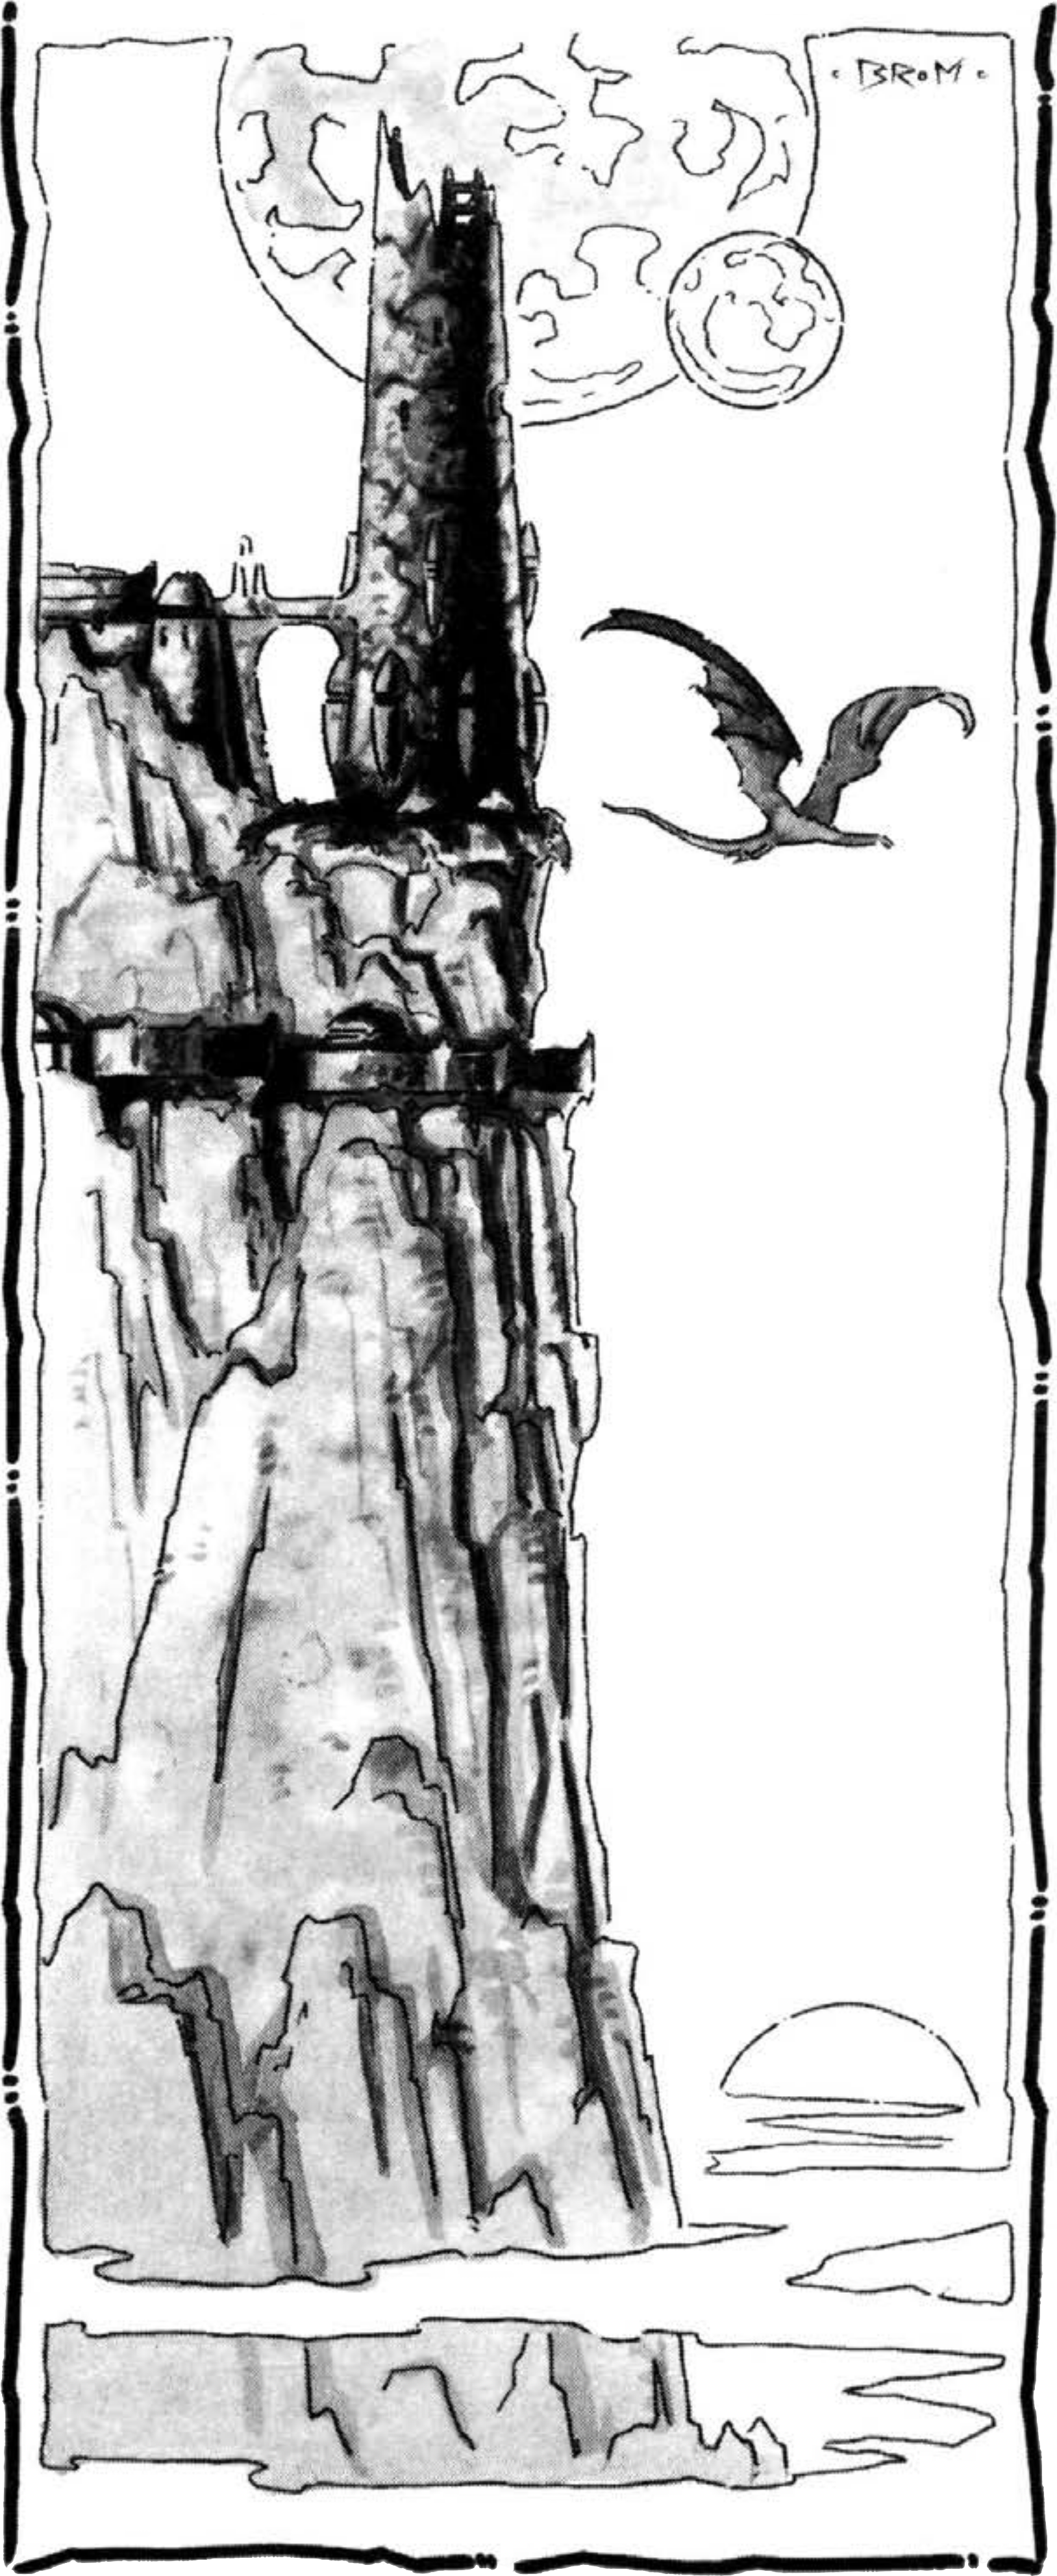
\includegraphics[width=\columnwidth]{images/tower-1.png}
\end{figure}
\Chapter{Abilities}
{Life is a mysterious and resilient thing. Even in the starkest wastes of Athas, the careful observer finds it clinging to the horns of sand dunes, peeking out from beneath wind-raked boulders, and creeping along the cracked plains of sun-baked clay.
To survive, almost every form of life has become a monster. On the increasingly infertile world of Athas, these adaptations have taken an almost diabolical turn. The land is so barren that every form of life, to one extent or another, is both predator and prey.}
{The Wanderer's Journal}

\Capitalize{E}{ach} character in {\tableheader Dark Sun} has six abilities: Strength (abbreviated Str), Dexterity (Dex), Constitution (Con), Intelligence (Int), Wisdom (Wis), and Charisma (Cha). Each of your abilities above average gives you a bonus on certain die rolls, and abilities below average give you a penalty on other die rolls.

\section{Ability Scores}

Previous editions used a rolling method that produced, on average, higher stats. This was supposed to convey that Athas was a much harsher world than normal D\&D campaign worlds, and that its denizens had adapted to compensate. However, the meaning of an attribute has changed in 3rd edition, and attributes start having a positive effect much sooner than they did in 2nd edition. Whereas many stats didn't start having a positive effect until they were at least 14, now as low as 12 have a positive effect. Using higher overall attributes for characters in {\tableheader Dark Sun} actually makes it easier for characters to survive and overcome obstacles that should be challenging, which would mean that the effective difficulty of a campaign would actually be lower using this stat generation method.

% \subsection{Creating Ability Scores}
% There are two methods for creating ability scores for your character: randomly or via point buy.  The average ability score for the typical commoner is 10 or 11, but your character is not typical. The most common ability scores for player characters (PCs) are 12 and 13.

% \subsubsection{Random Generation}
% To create an ability score for your character, roll 4d6. Disregard the lowest die roll and sum the rest. The result is a number between 3 (horrible) and 18 (tremendous)
% .
% Make this roll six times, recording each result on a piece of paper. Once you have six scores, assign each score to one of the six abilities.

% \subsubsection{Point Buy}
% All abilities scores start at 8. Take a number of points according to the type of your campaign to spread out among all abilities. For ability scores of 14 or lower, you buy additional points on a 1-for-1 basis. For ability scores higher than 14, it costs a little more.

% \Table{}{C C C C}{\tableheader Ability Score & \tableheader Point Cost & \tableheader Ability Score & \tableheader Point Cost \\
%   9 & 1 & 14 & 6 \\
%   10 & 2 & 15 & 8 \\
%   11 & 3 & 16 & 10 \\
%   12 & 4 & 17 & 13 \\
%   13 & 5 & 18 & 16}

% \Table{}{X r}{\tableheader Type of Campaign & \tableheader Points Allowed\\
%   Low-powered campaign & 15 points \\
%   Challenging campaign & 22 points \\
%   Normal campaign & 25 points \\
%   Tougher campaign & 28 points \\
%   High-powered campaign & 32 points}

\subsection{Ability Modifiers}

Each ability, after changes made because of race, has a modifier ranging from $-5$ to +5. \tabref{Ability Modifiers and Bonus Spells} shows the modifier for each score. It also shows bonus spells, which you'll need to know about if your character is a spellcaster.

The modifier is the number you apply to the die roll when your character tries to do something related to that ability. You also use the modifier with some numbers that aren't die rolls. A positive modifier is called a bonus, and a negative modifier is called a penalty.

\BigTable{Ability Modifiers and Bonus Spells}{X c C C C C C C C C C C}{
  \hline
  \rowcolor{white}
  & & \multicolumn{10}{c}{\tableheader Bonus Spells (by spell level)} \\
  \hline
  \rowcolor{white}
  \tableheader Score & \tableheader Modifier & \tableheader 0 & \tableheader 1st & \tableheader 2nd & \tableheader 3rd & \tableheader 4th & \tableheader 5th & \tableheader 6th & \tableheader 7th & \tableheader 8th & \tableheader 9th \\
  1 & $-5$ & \cellcolor{TableColor}&\cellcolor{TableColor}&\cellcolor{TableColor}&\cellcolor{TableColor}&\cellcolor{TableColor}&\cellcolor{TableColor}&\cellcolor{TableColor}&\cellcolor{TableColor}&\cellcolor{TableColor}&\cellcolor{TableColor}\\
  2-3 & $-4$ & \cellcolor{TableColor}&\cellcolor{TableColor}&\cellcolor{TableColor}&\cellcolor{TableColor}&\cellcolor{TableColor}&\cellcolor{TableColor}&\cellcolor{TableColor}&\cellcolor{TableColor}&\cellcolor{TableColor}&\cellcolor{TableColor}\\
  4-5 & $-3$ & \cellcolor{TableColor}&\cellcolor{TableColor}&\cellcolor{TableColor}&\cellcolor{TableColor}&\cellcolor{TableColor}&\cellcolor{TableColor}&\cellcolor{TableColor}&\cellcolor{TableColor}&\cellcolor{TableColor}&\cellcolor{TableColor}\\
  6-7 & $-2$ & \cellcolor{TableColor}&\cellcolor{TableColor}&\cellcolor{TableColor}&\cellcolor{TableColor}&\cellcolor{TableColor}&\cellcolor{TableColor}&\cellcolor{TableColor}&\cellcolor{TableColor}&\cellcolor{TableColor}&\cellcolor{TableColor}\\
  8-9 & $-1$ &\multicolumn{10}{c}{\multirow{-5}{*}{\bfseries Can't cast spells tied to this ability}}\\
  10-11 & 0 &&&&&&&&&&\\
  12-13 & +1 && 1 &&&&&&&&\\
  14-15 & +2 && 1 & 1 &&&&&&&\\
  16-17 & +3 && 1 & 1 & 1 &&&&&&\\
  18-19 & +4 && 1 & 1 & 1 & 1 &&&&&\\
  20-21 & +5 && 2 & 1 & 1 & 1 & 1 &&&&\\
  22-23 & +6 && 2 & 2 & 1 & 1 & 1 & 1 &&&\\
  24-25 & +7 && 2 & 2 & 2 & 1 & 1 & 1 & 1 &&\\
  26-27 & +8 && 2 & 2 & 2 & 2 & 1 & 1 & 1 & 1 &\\
  28-29 & +9 && 3 & 2 & 2 & 2 & 2 & 1 & 1 & 1 & 1 \\
  30-31 & +10 && 3 & 3 & 2 & 2 & 2 & 2 & 1 & 1 & 1 \\
  32-33 & +11 && 3 & 3 & 3 & 2 & 2 & 2 & 2 & 1 & 1 \\
  34-35 & +12 && 3 & 3 & 3 & 3 & 2 & 2 & 2 & 2 & 1 \\
  36-37 & +13 && 4 & 3 & 3 & 3 & 3 & 2 & 2 & 2 & 2 \\
  38-39 & +14 && 4 & 4 & 3 & 3 & 3 & 3 & 2 & 2 & 2 \\
  40-41 & +15 && 4 & 4 & 4 & 3 & 3 & 3 & 3 & 2 & 2
}

\BigTable{Ability Scores and Bonus Power Points}{l C C C C C C C C C C C C C C C C C C C C}{
  \hline
  \rowcolor{white}
  & \multicolumn{20}{c}{\tableheader Bonus Power Points (by class level)} \\
  \hline
  \rowcolor{white}
\tableheader Score & \tableheader 1st & \tableheader 2nd & \tableheader 3rd & \tableheader 4th & \tableheader 5th & \tableheader 6th & \tableheader 7th & \tableheader 8th & \tableheader 9th & \tableheader 10th & \tableheader 11th & \tableheader 12th & \tableheader 13th & \tableheader 14th & \tableheader 15th & \tableheader 16th & \tableheader 17th & \tableheader 18th & \tableheader 19th & \tableheader 20th \\
10-11 &&&&&&&&&&&&&&&&&&&&\\
12-13 && 1 & 1 & 2 & 2 & 3 & 3 & 4 & 4 & 5 & 5 & 6 & 6 & 7 & 7 & 8 & 8 & 9 & 9 & 10 \\
14-15 & 1 & 2 & 3 & 4 & 5 & 6 & 7 & 8 & 9 & 10 & 11 & 12 & 13 & 14 & 15 & 16 & 17 & 18 & 19 & 20 \\
16-17 & 1 & 3 & 4 & 6 & 7 & 9 & 10 & 12 & 13 & 15 & 16 & 18 & 19 & 21 & 22 & 24 & 25 & 27 & 28 & 30 \\
18-19 & 2 & 4 & 6 & 8 & 10 & 12 & 14 & 16 & 18 & 20 & 22 & 24 & 26 & 28 & 30 & 32 & 34 & 36 & 38 & 40 \\
20-21 & 2 & 5 & 7 & 10 & 12 & 15 & 17 & 20 & 22 & 25 & 27 & 30 & 32 & 35 & 37 & 40 & 42 & 45 & 47 & 50 \\
22-23 & 3 & 6 & 9 & 12 & 15 & 18 & 21 & 24 & 27 & 30 & 33 & 36 & 39 & 42 & 45 & 48 & 51 & 54 & 57 & 60 \\
24-25 & 3 & 7 & 10 & 14 & 17 & 21 & 24 & 28 & 31 & 35 & 38 & 42 & 45 & 49 & 52 & 56 & 59 & 63 & 66 & 70 \\
26-27 & 4 & 8 & 12 & 16 & 20 & 24 & 28 & 32 & 36 & 40 & 44 & 48 & 52 & 56 & 60 & 64 & 68 & 72 & 76 & 80 \\
28-29 & 4 & 9 & 13 & 18 & 22 & 27 & 31 & 36 & 40 & 45 & 49 & 54 & 58 & 63 & 67 & 72 & 76 & 81 & 85 & 90 \\
30-31 & 5 & 10 & 15 & 20 & 25 & 30 & 35 & 40 & 45 & 50 & 55 & 60 & 65 & 70 & 75 & 80 & 85 & 90 & 95 & 100 \\
32-33 & 5 & 11 & 16 & 22 & 27 & 33 & 38 & 44 & 49 & 55 & 60 & 66 & 71 & 77 & 82 & 88 & 93 & 99 & 104 & 110 \\
34-35 & 6 & 12 & 18 & 24 & 30 & 36 & 42 & 48 & 54 & 60 & 66 & 72 & 78 & 84 & 90 & 96 & 102 & 108 & 114 & 120 \\
36-37 & 6 & 13 & 19 & 26 & 32 & 39 & 45 & 52 & 58 & 65 & 71 & 78 & 84 & 91 & 97 & 104 & 110 & 117 & 123 & 130 \\
38-39 & 7 & 14 & 21 & 28 & 35 & 42 & 49 & 56 & 63 & 70 & 77 & 84 & 91 & 98 & 105 & 112 & 119 & 126 & 133 & 140 \\
40-41 & 7 & 15 & 22 & 30 & 37 & 45 & 52 & 60 & 67 & 75 & 82 & 90 & 97 & 105 & 112 & 120 & 127 & 135 & 142 & 150}

\subsection{Abilities, Spellcasters and \hskip4em Manifesters}
The ability that governs bonus spells depends on what type of spellcaster your character is: Intelligence for wizards; Wisdom for clerics, druids, and rangers; or Charisma for templars. In addition to having a high ability score, a spellcaster must be of high enough class level to be able to cast spells of a given spell level.

Psionic classes also depend on abilities for additional power: Intelligence for psions, Wisdom for psychic warriors, and Charisma for wilders. The modifier for this ability is referred to as your key ability modifier. If your character's key ability score is 9 or lower, you can't manifest powers from that psionic class.

Just as a high Intelligence score grants bonus spells to a wizard and a high Wisdom score grants bonus spells to a cleric, a character who manifests powers (psions, psychic warriors, and wilders) gains bonus power points according to his key ability score. Refer to \tabref{Ability Scores and Bonus Power Points}.

\subsubsection{How To Determine Bonus Power Points}
Your key ability score grants you additional power points equal to your key ability modifier $\times$ your manifester level $\times$ \onehalf. \tabref{Ability Scores and Bonus Power Points} shows these calculations for class levels 1st through 20th and key ability scores from 10 to 41.

\section{The Abilities}
Each ability partially describes your character and affects some of his or her actions.

\subsection{Strength (Str)}
Strength measures your character's muscle and physical power. This ability is especially important for gladiators, fighters, barbarians, and rangers because it helps them prevail in combat. Strength also limits the amount of equipment your character can carry.

You apply your character's Strength modifier to:
\begin{itemize*}
\item Melee attack rolls.
\item Damage rolls when using a melee weapon or a thrown weapon (including a sling). (Exceptions: Off-hand attacks receive only one-half the character's Strength bonus, while two-handed attacks receive one and a half times the Strength bonus. A Strength penalty, but not a bonus, applies to attacks made with a bow that is not a composite bow.)
\item \skill{Climb}, \skill{Jump}, and \skill{Swim} checks. These are the skills that have Strength as their key ability.
\item Strength checks (for breaking down doors and the like).
\end{itemize*}

\subsection{Dexterity (Dex)}
Dexterity measures hand-eye coordination, agility, reflexes, and balance. This ability is the most important one for rogues, and bards, but it's also high on the list for characters who typically wear light or medium armor (gladiators, rangers, wilders, and barbarians) or no armor at all (psions and wizards), and for anyone who wants to be a skilled archer.

You apply your character's Dexterity modifier to:
\begin{itemize*}
\item Ranged attack rolls, including those for attacks made with bows, crossbows, throwing axes, and other ranged weapons.
\item Armor Class (AC), provided that the character can react to the attack.
\item Reflex saving throws, for avoiding fireballs and other attacks that you can escape by moving quickly.
\item \skill{Balance}, \skill{Escape Artist}, \skill{Hide}, \skill{Move Silently}, \skill{Open Lock}, \skill{Ride}, \skill{Sleight of Hand}, \skill{Tumble}, and \skill{Use Rope} checks. These are the skills that have Dexterity as their key ability.
\end{itemize*}
\subsection{Constitution (Con)}
Constitution represents your character's health and stamina. A Constitution bonus increases a character's hit points, so the ability is important for all classes.

You apply your character's Constitution modifier to:
\begin{itemize*}
\item Each roll of a Hit Die (though a penalty can never drop a result below 1---that is, a character always gains at least 1 hit point each time he or she advances in level).
\item Fortitude saving throws, for resisting poison and similar threats.
\item \skill{Concentration} checks. Concentration is a skill, important to spellcasters, that has Constitution as its key ability.
\end{itemize*}

If a character's Constitution score changes enough to alter his or her Constitution modifier, the character's hit points also increase or decrease accordingly.

\subsection{Intelligence (Int)}
Intelligence determines how well your character learns and reasons. This ability is important for wizards because it affects how many spells they can cast, how hard their spells are to resist, and how powerful their spells can be. It's also important for any character who wants to have a wide assortment of skills.

You apply your character's Intelligence modifier to:
\begin{itemize*}
\item The number of languages your character knows at the start of the game.
\item The number of skill points gained each level. (But your character always gets at least 1 skill point per level.)
\item \skill{Appraise}, \skill{Craft}, \skill{Decipher Script}, \skill{Disable Device}, \skill{Forgery}, \skill{Knowledge}, \skill{Search}, and \skill{Spellcraft} checks. These are the skills that have Intelligence as their key ability.
\end{itemize*}

A wizard gains bonus spells based on her Intelligence score. The minimum Intelligence score needed to cast a wizard spell is 10 + the spell's level.

An animal has an Intelligence score of 1 or 2. A creature of human-like intelligence has a score of at least 3.

\subsection{Wisdom (Wis)}
Wisdom describes a character's willpower, common sense, perception, and intuition. While Intelligence represents one's ability to analyze information, Wisdom represents being in tune with and aware of one's surroundings. Wisdom is the most important ability for clerics and druids, and it is also important for rangers. If you want your character to have acute senses, put a high score in Wisdom. Every creature has a Wisdom score.

You apply your character's Wisdom modifier to:
\begin{itemize*}
\item Will saving throws (for negating the effect of charm person and other spells).
\item \skill{Heal}, \skill{Listen}, \skill{Profession}, \skill{Sense Motive}, \skill{Spot}, and \skill{Survival} checks. These are the skills that have Wisdom as their key ability.
\item Clerics, druids, and rangers get bonus spells based on their Wisdom scores. The minimum Wisdom score needed to cast a cleric, druid, or ranger spell is 10 + the spell's level.
\end{itemize*}

\subsection{Charisma (Cha)}
Charisma measures a character's force of personality, persuasiveness, personal magnetism, ability to lead, and physical attractiveness. This ability represents actual strength of personality, not merely how one is perceived by others in a social setting. Charisma is most important for templars. It is also important for clerics, since it affects their ability to turn undead. Every creature has a Charisma score.

You apply your character's Charisma modifier to:
\begin{itemize*}
\item \skill{Bluff}, \skill{Diplomacy}, \skill{Disguise}, \skill{Gather Information}, \skill{Handle Animal}, \skill{Intimidate}, \skill{Perform}, and \skill{Use Magic Device} checks. These are the skills that have Charisma as their key ability.
\item Checks that represent attempts to influence others.
\item Turning checks for clerics and templars attempting to turn zombies, vampires, and other undead.
\end{itemize*}

Sorcerers and bards get bonus spells based on their Charisma scores. The minimum Charisma score needed to cast a sorcerer or bard spell is 10 + the spell's level.

\subsection{Changing Ability Scores}
When an ability score changes, all attributes associated with that score change accordingly. A character does not retroactively get additional skill points for previous levels if she increases her intelligence.

\Chapter{Character Races}
{I live in a world of fire and sand. The crimson sun scorches the life from anything that crawls or flies, and storms of sand scour the foliage from the barren ground. Lightning strikes from the cloudless sky, and peals of thunder roll unexplained across the vast tablelands. Even the wind, dry and searing as a kiln, can kill a man with thirst.}
{The Wanderer's Journal}

\Capitalize{A}{thas} is a world of many races, from the gith who wander the deserts, to the tareks, too stubborn to know when they have died. Giants terrorize the Silt Sea, while belgoi steal grown men in the night. The magic of the Pristine Tower produces the New Races; most never see a second generation. Despite the variety of intelligent life, only a few races have the numbers to significantly impact the politics of the Tablelands.

Though the races of the {\tableheader Dark Sun} campaign setting resemble those of other campaign worlds, it is frequently in name only. The insular elves roam the Tablelands, trusted by no one but their own tribe-mates. Halflings are feral creatures, possessed of a taste for human flesh. Hairless dwarves work endlessly, their entire perception of the world filtered through the lens of a single, all-consuming task. Unsleeping thri-kreen roam the wastes, always hunting their next meal.

\section{Racial Characteristics}

\subsection{Ability Adjustments}

Find your character's race on \tabref{Athasian Racial Ability Adjustments} and apply the adjustments to your character's ability scores. If these changes put your score above 18 or below 3, that's okay, except in the case of Intelligence, which does not go below 3 for characters.

\subsection{Level Adjustment}

To determine the effective character level (ECL) of a character, add its race's level adjustment (LA) to its character class levels.

Use ECL instead of character level to determine how many experience points a character needs to reach its next level. Also use ECL to determine starting wealth for a character.

\subsection{Favored Class}

Each race's favored class is also given on \tabref{Athasian Racial Ability Adjustments}. A character's favored class doesn't count against him or her when determining experience point penalties for multiclassing.

\BigTablePair{Athasian Racial Ability Adjustments}{l l C p{6cm} p{2cm} l}{
\tableheader Race & \tableheader Type (Subtype) & \tableheader LA & \tableheader Ability Adjustments & \tableheader Favored Class & \tableheader Languages \\
Human & Humanoid (human) &&& Any & Common \\
Aarakocra & Monstrous Humanoid & +1 & $-2$ Strength, +4 Dexterity, $-2$ Charisma & Cleric & Auran, Common \\
Dwarf & Humanoid (dwarf) && +2 Constitution, $-2$ Charisma & Fighter & Common, Dwarven \\
Elf & Humanoid (elf) && +2 Dexterity, $-2$ Constitution & Rogue & Common, Elven \\
Half-elf & Humanoid (elf) && +2 Dexterity, $-2$ Charisma & Any & Common, Elven \\
Half-giant & Giant & +2 & +8 Strength, $-2$ Dexterity, +4 Constitution, \newline $-4$ Intelligence, $-4$ Wisdom, $-4$ Charisma & Barbarian & Common \\
Halfling & Humanoid (halfling) && $-2$ Strength, +2 Dexterity & Ranger & Halfling \\
Mul & Humanoid (dwarf) & +1 & +4 Strength, +2 Constitution, $-2$ Charisma & Gladiator & Common \\
Pterran & Humanoid (pterran) && $-2$ Dexterity, +2 Wisdom, +2 Charisma & Druid, ranger,\newline or telepath & Saurian \\
Thri-kreen & Monstrous Humanoid & +2 & +2 Strength, +4 Dexterity, $-2$ Intelligence, \newline +2 Wisdom, $-4$ Charisma & Psychic warrior & Kreen}

\subsection{Race And Languages}

Only races that live in the reach of the city-states know how to speak Common. A aarakocra, dwarf, elf, half-elf, halfling, pterran, or thri-kreen also speaks a racial language, as appropriate. A character who has an Intelligence bonus at 1st level speaks other languages as well, one extra language per point of Intelligence bonus as a starting character.

\textbf{Literacy}: The ability to read has been outlawed for thousands of years by the sorcerer-kings. All characters in a {\tableheader Dark Sun} campaign start without the ability to read or write.

\textbf{Class-Related Languages}: Clerics, druids, templars, and wizards can choose certain languages as bonus languages even if they're not on the lists found in the race descriptions. These class-related languages are as follows:

\textit{Cleric}: Aquan, Auran, Ignan, Terran.

\textit{Druid}: Sylvan.

\textit{Templar}: Templar's City-State language.

\textit{Wizard}: Draconic.

\section{Humans}
\Quote{Humans are fools, and hopelessly naive as well. They outnumber us; they are everywhere, and yet they have no more sense of their strength than a rat. Let us hope that the Datto remain that way.}{Dukkoti Nightrunner, elven warrior}

While not the strongest race, nor the quickest, humans have dominated the Tablelands for the last three thousand years.

\textbf{Personality:} More than other races, human personality is shaped by their social standing and background.

\textbf{Physical Description:} Human males average 1.8 meter tall and 100 kg, while smaller females average 1.65 meters and 70 kg. Color of eyes, skin, and hair, and other physical features vary wildly; enlarged noses, webbed feet or extra digits are not uncommon.

\textbf{Relations:} Human treatment of other races is usually based on what their culture has taught them. In large settlements, such as in city-states, close proximity with many races leads to a suspicious unfriendly tolerance.

\textbf{Alignment:} Humans have no racial tendency toward any specific alignment.

\textbf{Human Lands:} Humans can be found anywhere, from the great city-states to the barren wastes.

\textbf{Magic:} Most humans fear and hate arcane magic, forming mobs to kill vulnerable wizards.

\textbf{Psionics:} Humans see the Way as a natural part of daily life, and readily become psions.

\textbf{Religion:} Most humans pay homage to the elements. Draji and Gulgs often worship their monarchs.

\textbf{Language:} Most humans speak the common tongue. Nobles and artisans within a given city-state usually speak the city language, but slaves typically only speak Common.

\textbf{Names:} Nobles, artisans and traders use titles or surnames; others some simply use one name.

\textbf{Male Names:} Agis of Asticles, King Tithian, Lord Vordon, Pavek, Trenbull Al'Raam'ke

\textbf{Female Names:} Akassia, General Zanthiros, Lady Essen of Rees, Neeva, Sadira

\textbf{Adventurers:} Some human adventurers seek treasure; others adventure for religious purposes as clerics or druids; others seek companionship or simply survival.

\subsection{Human Racial Traits}
\begin{itemize*}
  \item Medium: As Medium creatures, humans have no special bonuses or penalties due to their size. 
  \item Human base land speed is 9 meters.
  \item 1 extra feat at 1st level.
  \item 4 extra skill points at 1st level and 1 extra skill point at each additional level.
  \item Automatic Language: Common. Bonus Languages: Any (other than secret languages, such as Druidic). See the \skill{Speak Language} skill.
  \item Favored Class: Any. When determining whether a multiclass human takes an experience point penalty, his or her highest-level class does not count.
\end{itemize*}

\section{Aarakocra}
\Quote{You are all slaves. You all suffer from the tyranny of the ground. Only in the company of clouds will you find the true meaning of freedom.}{Kekko Cloud-Brother, aarakocra cleric}

Aarakocra are the most commonly encountered bird-people of the Tablelands. Some are from Winter Nest in the White Mountains near Kurn, while others are from smaller tribes scattered in the Ringing Mountains and elsewhere. These freedom-loving creatures rarely leave their homes high in the mountains, but sometimes, either as young wanderers or cautious adventurers, they venture into the inhabited regions of the Tablelands.

\textbf{Personality:} These bird-people can spend hours riding the wind currents of the mountains, soaring in the olive-tinged Athasian sky. While traveling, aarakocra prefer to fly high above to get a good view all around their location and detect any threats well in advance. When they stop to rest, they tend to perch on high peaks or tall buildings. Enclosed spaces threaten the aarakocra, who have a racial fear of being anywhere they cannot stretch their wings. This claustrophobia affects their behavior. Unless it is absolutely necessary, no aarakocra will enter a cave or enclosed building, or even a narrow canyon.

\textbf{Physical Description:} Aarakocra stand 2 to 2.4 meters tall, with a wingspan of about 6 meters. They have black eyes, gray beaks, and from a distance they resemble lanky disheveled vultures. Aarakocran plumage ranges from silver white to brown, even pale blue. Male aarakocra weigh around 50 kg, while females average 42.5 kg. An aarakocra's beak comprises much of its head, and it can be used in combat. At the center of their wings, aarakocra have three-fingered hands with an opposable thumb, and the talons of their feet are just as dexterous. While flying, aarakocra can use their feet as hands, but while walking, they use their wing-hands to carry weapons or equipment. Aarakocra have a bony plate in their chest (the breastbone), which provides protection from blows. However, most of their bones are hollow and brittle and break more easily than most humanoids. The aarakocra's unusual build means they have difficulty finding armor, unless it has been specifically made for aarakocra. Aarakocra usually live between 30 and 40 years.

\textbf{Relations:} Aarakocra zealously defend their homeland. They are distrustful of strangers that venture onto their lands. Many of the southern tribes exact tolls on all caravans passing through their lands, sometimes kidnapping scouts or lone riders until tribute is paid. Tribute can take the form of livestock or shiny objects, which aarakocra covet. Some evil tribes may attack caravans without provocation. Aarakocra have great confidence and pride in their ability to fly, but have little empathy for land-bound races.

\textbf{Alignment:} Aarakocra tend towards neutrality with regard to law or chaos. With respect to good and evil, Aarakocran tribes usually follow the alignment of their leader. A tribe whose leader is neutral good will contain lawful good, neutral good, chaotic good and neutral members, with most members being neutral good. Aarakocra, even good ones, rarely help out strangers.

\textbf{Aarakocran Lands:} Most Aarakocran communities are small nomadic tribes. Some prey on caravans, while others or build isolated aeries high in the mountains. The least xenophobic aarakocra generally come from Winter Nest, in the White Mountains, a tribe allied with the city-state of Kurn. Of all the human communities, only Kurn builds perches especially made for aarakocra to rest and do business. In contrast, king Daskinor of Eldaarich has ordered the capture and extermination of all aarakocra. Other human communities tolerate Aarakocran characters but do not welcome them. Merchants will do business with aarakocra as long as they remain on foot. Most land-bound creatures are suspicious of strange creatures that fly over their herds or lands unannounced, and templars, even in Kurn, have standing orders to attack creatures that fly over the city walls without permission.

\textbf{Magic:} Most Aarakocran tribes shun wizardly magic, but a few evil tribes have defilers, and one prominent good-aligned tribe, Winter's Nest, has several preservers.

\textbf{Psionics:} Aarakocra are as familiar with psionics as other races of the tablelands. They particularly excel in the psychoportation discipline. In spite of their low strength and constitutions, they excel as psychic warriors, often using ranged touch powers from above to terrifying effect.

\textbf{Religion:} Aarakocran shamans are usually air clerics, sometimes sun clerics, and occasionally druids. Most rituals of Aarakocran society involve the summoning of an air elemental, or Hraak'thunn in Auran (although an aarakocra would call their language Silvaarak, and not Auran). Summoned air elementals are often used in an important ritual, the Hunt. The Aarakocran coming of age ceremony involves hunting the great beasts found in the Silt Sea.

\textbf{Language:} Athasian aarakocra speak Auran. Aarakocra have no written language of their own, though some of the more sophisticated tribes have borrowed alphabets from their land-bound neighbors. Regardless of the language spoken, aarakocra do not possess lips, and therefore cannot even approximate the 'm', 'b' or 'p' sounds. They have difficulty also with their 'f's and 'v's, and tend to pronounce these as 'th' sounds.

\textbf{Male Names:} Akthag, Awnunaak, Cawthra, Driikaak, Gazziija, Kraah, Krekkekelar, Nakaaka, Thraka.

\textbf{Female Names:} Arraako, Kariko, Kekko, Lisako, Troho.

\textbf{Tribal Names:} Cloud Gliders, Sky Divers, Peak Masters, Far Eyes, Brothers of the Sun.

\textbf{Adventurers:} Adventuring aarakocra are usually young adults with a taste for the unknown. They are usually curious, strong-minded individuals that wish to experience the lives of the land-bound peoples. Good tribes see these young ones as undisciplined individuals, but can tolerate this behavior. Evil tribes may view this sort of adventurous behavior as treacherous, and may even hunt down the rogue member.

\subsection{Aarakocra Society}
The aarakocra have a tribal society. The civilized tribes of Winter Nest form the largest known community of aarakocra in the Tyr region. Though their communities are lead by a chieftain, the aarakocra have a great love of personal freedom. So while the chieftain makes all major decisions for the community, unless she consults with the tribal elders and builds a strong consensus within the tribe first, her decisions may be ignored.

Air and sun shamans play an important role in aarakocra societies. Aarakocra worship the sun because it provides them with the thermals they need to soar. The air shamans of Winter Nest lead their community in daily worship of the air spirits.

Aarakocra of Winter Nest have a deep and abiding respect for the gifts of nature and little patience for those who abuse those gifts. They look after the natural resources of the White Mountains and have been known to punish those who despoil or abuse them.

In more primitive societies, female aarakocra rarely travel far from the safety of the nest, and focus solely on raising the young. In Winter Nest, both sexes participate in all aspects of society, with females more often elected by the elders to be chieftains.

Aarakocra believe that their ability to fly makes them superior to all other races and thus they have great confidence and pride in themselves. Though they often express sympathy for people unable to fly, this more often comes across as condescending.

Aarakocra are carnivores, but do not eat intelligent prey.
\subsection{Roleplaying Suggestions}
Loneliness doesn't bother you like it bothers people of other races. You loathe the heat and stink of the cities, and long for cold, clean mountain air. The spectacle and movement of so many sentient beings fascinates you, but watching them from above satisfies your curiosity. The very thought of being caught in a crowd of creatures, pinned so tight that you can't move your own wings, fills you with terror.

You are friendly enough with people of other races, provided they respect your physical distance, and are willing to be the ones that approach you. You form relationships with individuals, but don't involve yourself in the politics of other racial communities - in such matters you prefer to watch from above and to keep your opinions to yourself unless asked.

You prefer to enter buildings through a window rather than through a door. Your instincts are to keep several scattered, hidden, nests throughout the areas that you travel regularly: one never knows when one might need a high place to rest. Remember your love of heights and claustrophobia, and rely on Aarakocran skills and tactics (dive-bombing). Take advantage of your flying ability to scout out the area and keep a ``bird's eye view'' of every situation.

\subsection{Aarakocra Racial Traits}
\begin{itemize*}
    \item $-2$ Strength, +4 Dexterity, $-2$ Constitution: Aarakocra have keen reflexes, but their lightweight bones are fragile.
    \item Monstrous Humanoid: Aarakocra are not subject to spells or effects that affect humanoids only, such as charm person or dominate person.
    \item Medium: As Medium creatures, aarakocra have no special bonuses or penalties due to size.
    \item Low-light vision: Aarakocra can see twice as far as a human in moonlight and similar conditions of poor illumination, retaining the ability to distinguish color and detail.
    \item Aarakocra base land speed is 6 meters, and can fly with a movement rate of 27 meters (average maneuverability).
    \item +6 racial bonus to \skill{Spot} checks in daylight. Aarakocra have excellent vision.
    \item Natural Armor: Aarakocra have +1 natural armor bonus due to their bone chest plate that provides some protection from blows.
    \item Natural Weaponry: An aarakocra can rake with its claws for 1d3 points of damage, and use its secondary bite attack for 1d2 points of damage.
    \item Claustrophobic: Aarakocra receive a $-2$ morale penalty on all rolls when in an enclosed space. Being underground or in enclosed buildings is extremely distressing for them.
    \item Aerial Dive: Aarakocra can make dive attacks. A dive attack works just like a charge, but the diving creature must move a minimum of 9 meters. If attacking with a lance, the aarakocra deals double damage on a successful attack. Optionally, the aarakocra can make a full attack with its natural weapons (two claws and one bite) at the end of the charge, dealing normal damage.
    \item Automatic Languages: Auran and Common. Bonus Languages: Elven, Gith, and Saurian. Aarakocra often learn the languages of their allies and enemies.
    \item Favored Class: Cleric. A multiclass aarakocra's cleric class does not count when determining whether he takes an experience point for multiclassing.
    \item Level Adjustment: +1. Aarakocra are slightly more powerful and gain levels more slowly than most of the humanoid races of the Tablelands.
\end{itemize*}
\section{Dwarves}
\Quote{The worst thing you can say to a dwarf is 'It can't be done.' If he's already decided to do it, he may never speak to you again. If he hasn't decided to take up the task, he may commit imself to it simply out of spite. 'Impossible' is not a concept most dwarves understand. Anything can be done, with enough determination.}{Sha'len, Nibenese trader}

Dwarves form a good part of the people encountered in the Tablelands. These strong and devoted beings live to fulfill their focus, a task they choose to devote their lives to. Stubborn and strong-minded, dwarves make good companions, even though their usual focused nature can tend to be bothersome.

\textbf{Personality:} Dwarves prefer to occupy themselves with meaningful tasks, and often approach these tasks with an intensity rarely seen in other races. As such, dwarves make excellent laborers, and take great pride in their accomplishments. However, their stubbornness can lead to difficulties. Dwarves will sometimes fail to listen to reason, attempting to accomplish what are impossible tasks. Dwarves live for their focus. Dwarves that die while being unable to complete their focus return from the dead as banshees to haunt their unfinished work. A dwarf also rarely divulges his focus to anyone.

\textbf{Physical Description:} The dwarves of the Tablelands stand 1.35 m to 1.5 m tall, with big muscular limbs and a strong build. They weigh on average 100 kg. Dwarves are hairless, and find the very idea of hair repulsive. They have deeply tanned skin, and rarely decorate it with tattoos. Dwarves can live up to 250 years.

\textbf{Relations:} A dwarf's relation with others is often a function of his focus. People that help the dwarf accomplish his focus or share his goals are treated with respect and considered good companions. There is little room for compromise, though, with those that disagree with the dwarf's focus. If they hinder the dwarf, they are considered obstacles that must be removed. Community is important to the dwarves. Dwarves have a very strong racial affinity. They rarely share their history with non-dwarves; it can take years for a stranger to gain enough trust to be admitted into a Dwarven family circle.

\textbf{Alignment:} Dwarves tend towards a lawful alignment, with most members either good or neutral. Their devotion to following the established hierarchy in their village means they tend to follow the rules, sometimes to the point of ridicule.

\textbf{Dwarven Lands:} There are three main Dwarven settlements in the Tablelands: Kled, located near the city-state of Tyr, and the twin villages of North and South Ledopolus located in the southwestern edge of the Tablelands. Some Dwarven communities have developed in the city-states and in some small villages, while other dwarves have taken up residence with the slave tribes of the wastes.

\textbf{Magic:} Like most peoples, dwarves have an aversion to wizardly magic, and they are the least amenable to changing their minds about anything. Dwarves rarely take to the wizardly arts; the few that do are usually shunned from respectable Dwarven society. Some dwarves will travel with a wizard who proves himself a worthy companion, but few dwarves will truly ever trust a wizard.

\textbf{Psionics:} Like almost everything that they do, dwarves take to psionics with a vengeance. They make formidable egoists and nomads.

\textbf{Religion:} Dwarven communities are ruled by their elders; dwarves are particularly devoted to their community leader, the Urhnomous. Dwarves typically worship elemental earth. Fire is sometimes worshiped for its destructive power and water for its healing nature. Air's intangibility and chaotic nature attracts few Dwarven worshipers. Dwarven druids are unusual, and tend to devote themselves to a particular area of guarded land.

\textbf{Language:} Dwarves have a long and proud oral history. They have an old written language, but this is mostly used for writing histories. Dwarves will not teach their ancient language to outsiders, they prefer to keep that knowledge to themselves. The Dwarven language is deep and throaty, composed of many guttural sounds and harsh exclamations. Most non-dwarves get raw throats if they try to speak Dwarven for more than a few hours.

\textbf{Names:} A dwarf's name is usually granted to him by his clan leader after he completes his first focus.

\textbf{Male Names:} Baranus, Biirgaz, Bontar, Brul, Caelum, Caro, Daled, Drog, Fyra, Ghedran, Gralth, Gram, Jurgan, Lyanius, Murd, Nati, Portek.

\textbf{Female Names:} Ardin, Erda, Ghava, Greshin, Gudak, Lazra, N'kadir, Palashi, Vashara.

\textbf{Adventurers:} Dwarves adventure for different reasons. Sometimes they may adventure in order to learn about the Tablelands, although these curious adventurers tend to be young and brash. Many adventuring dwarves travel the Tablelands to complete their focus because sometimes a task may take them away from their communities. Some search for ancient Dwarven villages and the treasures they contain.

\subsection{Dwarf Society}
No dwarf is more content than while working toward the resolution of some cause. This task, called a focus, is approached with single-minded direction for the dwarf's entire life, if need be, though most focuses require considerable less time.

Free dwarves form communities based on clans, and are much focused on family. Ties of blood are honored and respected above all others, except the focus. Family honor is important to every dwarf, because an act that brings praise or shame in one generation is passed down to the family members of the next generation. There is no concept in the minds of dwarves of not following these family ties.

Dwarven communities are found in many types of terrain, from mountains and deserts to near human cities. Most communities are small, rarely exceeding 300 members and are usually formed of extended families linked by a common ancestor. Community leaders are called Urhnomous (over-leader). Each clan is lead by an uhrnius (leader).

Most free dwarves earn their money through trade. Those that stand out in this category are Dwarven metal smiths and mercenaries. Most Athasians acknowledge Dwarven forged metal to be among the best. Some dwarves even act as metal scavengers, seeking steel scraps where ever they can be found to sell to the smiths. Dwarven mercenaries are highly prized because once their loyalty is purchased it is never changed.

\subsection{Roleplaying Suggestions}
Remember the intensity of your focus. Breaking or ignoring a focus has social, philosophical and spiritual repercussions. For someone to stand in the way of your focus is an assault on you. There is no greater satisfaction than fulfilling a difficult focus. Keep a serious, sober attitude nearly always. The only time you show your festive side is when you have recently fulfilled a focus, during the hours or days until you set a new focus.

Only during these brief days of fulfillment, and only to other dwarves and your most trusted non-Dwarven friends, do you show your full joy and sense of humor. But these days are also a time of vulnerability, for until you set a new focus you lose all of your special focus-related bonuses.

\subsection{Dwarven Focus}

A dwarf's focus is the central point of his existence. Nothing is more rewarding to a dwarf than to complete his focus. A focus must take at least a week to complete; anything less than that is too simple a task to be considered a focus. Dwarves receive a morale bonus working to complete a focus. The task must be directly related to the completion of the focus, however.

For example, Grelak, protector of his Dwarven community, makes the retrieval of a sacred book stolen during a raid his focus. After a week of gathering clues, he sets out to retrieve the artifact from its current possessor, who hides in a trading post two weeks away. On the way to the outpost, he encounters a wild lirr; while battling this foe, he receives his morale bonus, because he is trying to reach the book. Later, Grelak stops in Nibenay for some rest, and gets in a brawl. He doesn't receive any bonuses, because he isn't actively pursuing his focus.

\subsection{Dwarf Racial Traits}
\begin{itemize*}
    \item +2 Constitution, $-2$ Charisma: Dwarves are strong and sturdy, but their single-mindedness hinders them when dealing with others.
    \item Humanoid (dwarf): Dwarves are humanoid creatures with the dwarf subtype.
    \item Medium: As Medium creatures, dwarves have no special bonuses or penalties due to size.
    \item Darkvision: Dwarves can see in the dark up to 18 meters. Darkvision is black and white only, but it is otherwise like normal sight, and dwarves can function just fine with no light at all.
    \item Dwarven base land speed is 6 meters. However, dwarves can move at this speed even when wearing medium or heavy armor or when carrying a medium or heavy load (unlike other creatures whose speed is reduced in such situations).
    \item Stability: A dwarf gains a +4 bonus on ability checks made to resist being bull rushed or tripped when standing on the ground (but not when climbing, flying, riding, or otherwise not standing firmly on the ground).
    \item +2 racial bonus on saving throws against poison.
    \item Weapon Familiarity: To dwarves, the urgrosh is treated as a martial rather than exotic weapon.
    \item +2 racial bonus on saving throws against spells and spell-like effects.
    \item +1 morale bonus on all checks directly related to their focus. This includes a skill bonus, an attack bonus, a damage bonus, or a saving throw bonus, or even a bonus to manifestation or spell save DCs.
    \item Automatic Languages: Common and Dwarven. Bonus Languages: Elven, Giant, Gith, Kreen, Saurian.
    \item Favored Class: Fighter. A multiclass dwarf's fighter class does not count when determining whether he takes an experience point for multiclassing.
\end{itemize*}
\section{Elves}
\Quote[-.7em]{Honor? The word does not exist in the elven language.}{Tharak, human guard}

Athas' deserts, plains, steppes and badlands are home to the elves, a long-limbed race of trading, raiding, thieving sprinters. Running is the key to acceptance and respect among elves. Elves that are injured and cannot run are often left behind to die.

\textbf{Personality:} Other races see elves as dishonest and lazy; generally a fair assessment. Elves idle around their time for days until compelled by need to exert themselves, but they can run for days without complaint. No self-respecting elf will consent to ride an animal. To do so is dishonorable; elven custom dictates that individuals keep up or be left behind. Elves prefer to lead short, happy lives rather than long, boring ones. Seeing the future as a dark, deadly place, they prefer to live in ``the now,'' enjoying each fleeting moment. They thrive in open spaces, and tend to wither in captivity.

\textbf{Physical Description:} Elves stand between 1.8 and 2.1 meters tall, with lean builds; angular, deeply etched features; and no facial hair. They dress in garb designed to protect from the desert and elements.

\textbf{Relations:} Elves tend to keep to their own tribe and their proven friends unless they have some sort of an angle - something to sell, or some deception to pass off. Strangers are potential enemies waiting to take advantage of them, so elves look for every opportunity to win the advantage. If an elf believes that a companion might make a worthy friend, the elf devises a series of ``tests'' of trust that allow the companion to prove that their friendship is ``stronger than the bonds of death,'' as elves say. Once a stranger has gained an elf's trust, he is forever that elf's friend. If this trust is ever betrayed, it is gone forever.

\Figure*{t}{images/elf-1.png}

\textbf{Alignment:} Elves tend towards chaos because of their love of freedom, variety and self-expression. With respect to good and evil, elves tend towards neutrality, although their behavior leans towards chaos because of their love of freedom. With respect to good and evil, elves tend towards neutrality, although their behavior leans towards good - even self-sacrifice---where the good of their tribe is at stake. Although they'll steal everything in sight, elves are not murderous. They rarely attack anyone except those who threaten them or stand in their way.

\textbf{Elven Lands:} Always at home when running in the wastes, elves often act as if all plains and badlands were elven lands. However, since most elves are loath to settle or build, they can rarely enforce their claims. Elven tribes make a living either through herding, raiding or trading; most tribes have at one time or another plied their hand at all three of these occupations. A tribe's current occupation usually determines which lands they currently claim as their own. Elven herders claim grazing lands. Elven raiders claim lands crossed by trade routes. Elven traders claim no lands, but wander in search of bargains and loose purses.

\textbf{Magic:} Of all Tableland races, elves have the greatest affinity towards and acceptance of arcane practices.

\textbf{Psionics:} Persistence is not an elven strong suit, so elven Will is often weaker than that of other races. A few elves study the Way to win one more advantage in battle and trade.

\textbf{Religion:} Elves revere Coraanu Star Racer as the ideal ``First Elf - the warrior thief'' the embodiment of all that elves wish to be, basing their calendar on his life and honoring his myth with exquisite song, dance and celebration. Many elves worship the elements; particularly air, which they associate with freedom, swiftness and song. Elves also honor and swear by the moons, perhaps because low-light vision turns moonlight into an elven advantage.

\textbf{Language:} Elves of Athas share a common language and can communicate easily with each other, although each tribe has its own distinct dialect. The elven language is filled with short, clipped words, runs with a rapid staccato pace and is difficult for novices to pick up. Disdaining the slow tedious languages of other races most elves condescend to learn the Common speech for trade. Elves that learn other tongues often hide their ability.

\textbf{Names:} Whether slave or free, elves prefer to keep elven names. Tribe members take the tribe name as surname. Elves treat the naming of young runners as a sacred responsibility, naming the children of the tribe after the first interesting thing that they do while learning to run. Elves believe with the appropriate name, a child can grow to greatness, but with the wrong name, the elf may vanish in the wastes. Sometimes a child's name is changed because of an extraordinary deed performed during an elf's rite of passage.

\textbf{Male Names:} Botuu (Water Runner), Coraanu (First Elf, the Warrior Thief), Dukkoti (Wind Fighter), Haaku (Two Daggers), Lobuu (First Runner), Mutami (Laughs at Sun), Nuuko (Sky Hunter), Traako (Metal Stealer).

\textbf{Female Names:} Alaa (Bird Chaser), Ekee (Wild Dancer), Guuta (Singing Sword), Hukaa (Fire Leaper), Ittee (Dancing Bow), Nuuta (Quiet Hunter), Utaa (Laughing Moon)

\textbf{Tribe (Clan) Names:} Clearwater Tribe (Fireshaper, Graffyon, Graystar, Lightning, Onyx, Sandrunner, Seafoam, Silverleaf, Songweaver, Steeljaw, Wavedivers, Windriders clans); Night Runner Tribe (Dark Moons, Full Moons, Half Moons, Lone Moons, New Moons, Quarter Moons clans); Shadow Tribe; Silt Stalker Tribe (Fire Bow, Fire Dagger, Fire Sword clans); Silver Hand Tribe; Sky Singer Tribe (Dawnchaser, Dayjumper, Twilightcatcher clans); Swiftwing Tribe; Water Hunter Tribe (Raindancer, Poolrunner, Lakesinger clans); Wind Dancer Tribe (Airhunter, Breezechaser clans)

\textbf{Adventurers:} Elves often take up adventuring out of wanderlust, but those that persist in adventuring generally do so out of desire for profit, glory, revenge, or out of loyalty to traveling companions who have won their friendship. Elves love to boast of their accomplishments or have their deeds woven into song. Elves often hoard keepsakes from a memorable raids; some quilt pieces of stolen clothing into their cloaks. Little pleases elves as much as to flaunt a stolen item in front of its original owner. Elven custom dictates that the victim should acknowledge the accomplishment by congratulating the thief on his possession of such an attractive item. Those who fail to show such gallantry are considered poor sports. Adventurers who keep their tribal membership should give their chief periodic choice of the treasure that they have won. Holding out on a chief suggests lack of loyalty to the tribe.

\subsection{Elf Society}
Elves have an intense tribal unity that does not extend beyond their own tribe. Elves from other tribes are considered potential enemies as much as any other creature. Within a tribe all elves are considered equal with one exception, the chief. The chief rules for life and makes the major decisions concerning the tribe. The method of choosing the chief varies from tribe to tribe, with some electing the individual who demonstrates qualities of leadership the most while, the leadership in other tribes is inherited by the descendants of the previous chief. Elves do not spend vast amounts of time huddled in conference or following their chief's orders. Their love of freedom keeps elves from becoming embroiled in the complicated court intrigues that other races face. They prefer to engage in intrigues directed against outsiders.

Only with considerable effort and intent can a stranger become accepted by an elf tribe or even an individual elf. The stranger must show bravery and a willingness to sacrifice for the elf to earn acceptance. Being an elf does not increase a stranger's chances of being accepted by a tribe.

When in the company of outsiders, elves create tests of trust and friendship constantly for their companions. This continues until either the companions fail a test, in which case they will never earn the elf's trust, or they succeed in passing enough tests to convince the elf to accept them.

Years of conditioning have instilled within all elves the ability to move quickly over sandy and rocky terrain and run for long distances. Because of this natural maneuverability, elves spurn the riding of beasts for transportation. To do so is dishonorable. The elven custom is to keep up on one's own or be left behind.

Elven culture is rich and diverse, with elf song and dance being the most captivating in the Tablelands. They have turned celebrating into an art form. Elven songs and celebrations revolve around heroes of the tribe both ancient and current members. When a hunt goes well, a tribe showers the hunt master with praise. To celebrate a marriage, elves dance to the tales of long remembered lovers.

Elves have the reputation as being lazy and deceitful, which in most cases is true. They desire to lead short, happy lives as opposed to long, sad ones. This leads the elves to focus on the present rather than plan for or expect consequences in the future.

However, elves do work. Thought most elves provide for themselves and their tribe through herding, all elves have a propensity for raiding. Others become merchants and some thieves. In many cases, others find it difficult to see the distinction. Though they detest hard labor, elves will spend hours negotiating with potential customers.

\subsection{Roleplaying Suggestions}
Rely on elven combat skills (distance, bows, and fighting by the light of the moons and stars). Use elven noncombat skills and philosophy (running, escape from entangling situations or relationships). When someone professes to be your friend, dismiss them at first and then later, offer them a test of trust. Don't tell them that it is a test, of course. Ask them to give you one of their prize possessions, for example, or leave your own valuables out and see if they take advantage of you. Pretend to sleep, and find out what they say about you when they think you are not listening. Some elves go as far as to allow themselves to be captured to see if the presumed friend will rescue them!

\subsection{Elf Racial Traits}
\begin{itemize*}
    \item +4 Dexterity, $-4$ Constitution, +2 Intelligence, $-2$ Wisdom: Elves are agile and more intelligent, but they are less resilient than humans.
    \item Humanoid (elf): Elves are humanoid creatures with the elf subtype.
    \item Medium: As Medium creatures, elves have no special bonuses or penalties due to size.
    \item Elven base land speed is 9 meters.
    \item Enhanced Land Speed: Elves gain +1.5 m racial bonus to their land speed for each bonus on Dexterity above +1 (+1.5 m at +2 bonus, +3 m at +3 bonus, +4.5 m at +4 bonus, and so on).
    % \item Low-Light vision: Elves can see twice as far as a human in moonlight and similar conditions of poor illumination, retaining the ability to distinguish color and detail.
    \item Darkvision: Elves can see in the dark up to 18 meters. Darkvision is black and white only, but it is otherwise like normal sight, and elves can function just fine with no light at all.
    \item +1 racial bonus on attack rolls made with long swords and longbows.
    \item +2 racial bonus on initiative rolls.
    % \item Proficient with all bows.
    \item Weapon Familiarity: Elven longblade. All elves treat the elven longblade as a martial weapon.
    % \item +2 racial bonus to \skill{Listen}, \skill{Perform}, \skill{Search} and \skill{Spot} checks. Elves have keen senses.
    \item +5 racial bonus to \skill{Diplomacy} checks made for bargaining. Elves are notoriously skilled in haggling.
    \item Elves have a natural resistance to sever temperatures and aren't adversely affected by the heat of the day or the chill of the night. They treat extreme heat (61 °C to 82 °C) or extreme cold ($-45$ °C to $-29$ °C) as if it were only hot or cold, but suffer normally from unearthly heat (83 °C to 99 °C) or burning heat (100 °C or higher), or from magical supernatural heat and cold.
    % \item Elf Run: After a minute of warm-up and a \skill{Autohypnosis} check (DC 10), elves can induce an elf run state. This state allows elves to hustle for long distances as easily as a human can move normally, and run for long distances as easily as a human can hustle. Each day that an elf continues the elf run, he must make additional \skill{Autohypnosis} checks to maintain his elf run state: A trivial check (DC 10) on the second day, an easy check (DC 15) on the third day, an average check (DC 20) on the fourth day, a difficult check (DC 30) on the fifth day, and a heroic check (DC 40) on the sixth day. Once the elf fails his \skill{Autohypnosis} check, he loses the elf run benefits and suffers normal penalties for extended hustling and running. After a full day's rest, the elf may attempt again to induce an elf run state. With a group of elves, runners add their leader's Charisma bonus both to their movement rate and to any Fortitude checks related to movement.
    \item Elf Run: With one full-round of preparation, an elf adds 1\onehalf $\times$ his Constitution score in kilometers to his daily overland movement, or \onehalf $\times$ his Constitution score in kilometers to his hustle movement. To determine how many days the elf can maintain the state of elf run, he must roll a Constitution check and compare with the following table:

    \Table{}{z{35mm}z{35mm}}{
        \tableheader Constitution Check DC & \tableheader Days Before Penalties \\
        18 & 7 \\
        15 & 6 \\
        12 & 5 \\
         9 & 4 \\
         5 & 3 \\
         0 & 2 \\
    }

    Failure in this test or not preparing for the elf run means the elf can still run for one whole day before the penalties apply. After this period, if the elf continues to run he becomes fatigued and takes nonlethal damage as if he was hustling (see \chapref{Adventuring}). An elf fatigued because of the elf run must rest for a full day to recover. A fatigued elf cannot start an elf run.

    \item Mass Elf Run: Three or more elves can take one hour to prepare for an elf run. The whole elven group adds 1\onehalf $\times$ the group leader's Constitution score plus the group leader's Charisma bonus (if any) in kilometers to their daily overland movement. In order to determine how many days the group can maintain the elf run, they roll a single Constitution check for the whole group. They use the leader's Constitution modifier plus the leader's Charisma modifier. The group leader is not necessarily who has better Constitution score.
    \item Automatic Languages: Common and Elven. Bonus Languages: Dwarven, Entomic, Kreen, Gith, Saurian, and Terran.
    \item Favored Class: Ranger or Wizard. An elf must choose between ranger or wizard as favored class. This choice cannot be changed. A multiclass elf's chosen class does not count when determining class prerequisites for multiclassing.
\end{itemize*}

\vskip2cm
\section{Half-Elves}
\Quote{People are no good. You can only trust animals and the bottle.}{Delmao, half-Elven thief}

\begin{figure}[b!]
\centering
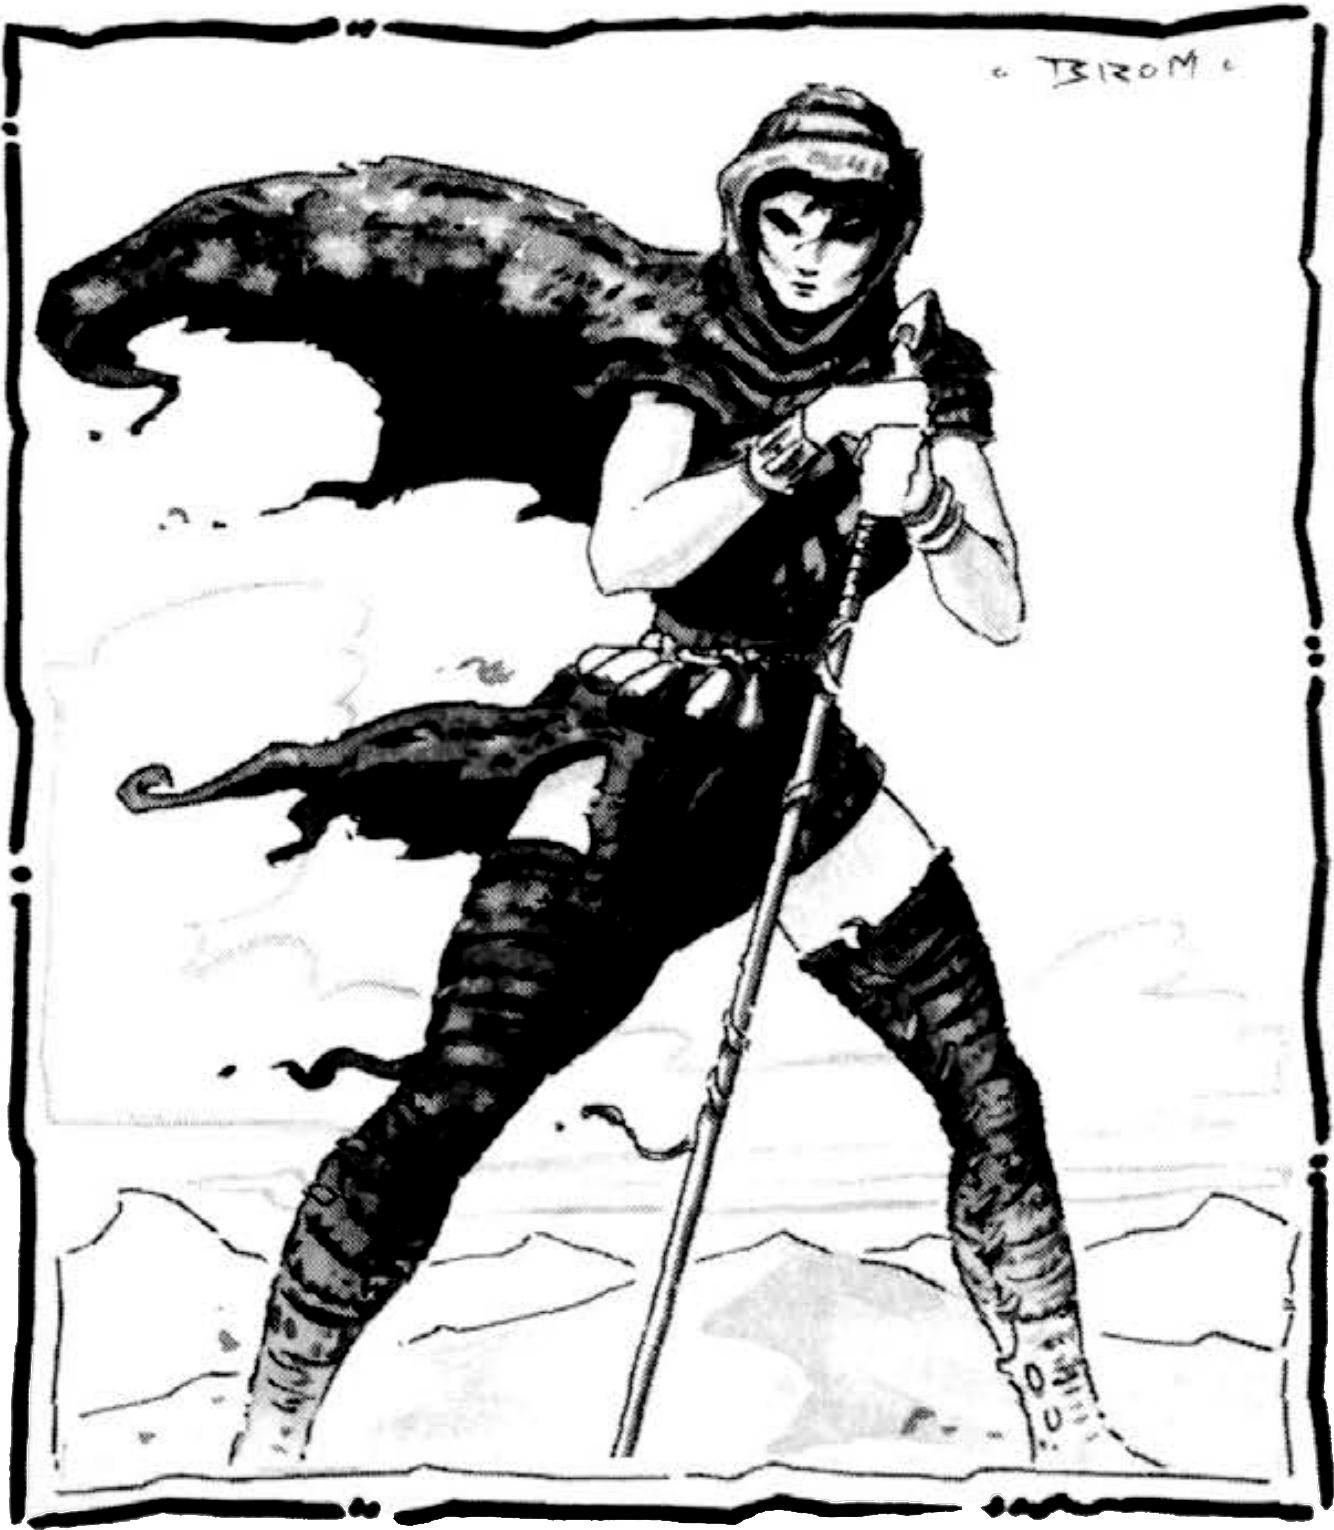
\includegraphics[width=\columnwidth]{images/halfelf-1.png}
\end{figure}
Unlike the parents of muls, elves and humans are often attracted to each other. Half-elves are typically the unwanted product of a casual interracial encounter.

\textbf{Personality:} Half-elves are notorious loners. Many Athasians believe that half-elves combine the worst traits of both races, but the most difficult aspect of half-elves---their lack of self-confidence comes not from their mixed origins but rather from a life of rejection from both parent races. Half-elves try in vain to gain the respect of humans or elves.

\textbf{Physical Description:} Averaging over 1.8 meters tall, half-elves combine Elven dexterity with human resilience. Bulkier than elves, most half-elves find it easier to pass themselves off as full humans than as full elves, but all have some features that hint at their Elven heritage.

\textbf{Relations:} Humans distrust the half-elf's Elven nature, while elves have no use for their mixed-blood children; Elven traditions demand that such children be left behind. Human society gives half-elves have a better chance of survival, but even less kindness. Half-elves sometimes find friendship among muls or even Thri-kreen. Half-elves will cooperate with companions when necessary, but find it difficult to rely on anyone. Many half-elves also turn to the animal world for company, training creatures to be servants and friends. Ironically, the survival skills and animal affinity that half-elves developed to cope with isolation make them valuable beast handlers in human society.

\textbf{Alignment:} Lawful and neutral half-elves labor for acceptance from a parent race, while chaotic ones have given up on acceptance, electing instead to reject the society that has rejected them.

\textbf{Half-Elven Lands:} Despite their unique nature, half-elves don't form communities. The few half-elves that settle down tend to live among humans who, unlike elves, at least find a use for them.

\textbf{Magic:} Half-elves often take up arcane studies, because it is a solitary calling.

\textbf{Psionics:} Mastery of the Way often provides the independence and self-knowledge that half-elves seek, and membership in a psionic academy can provide the half-elf with acceptance.

\textbf{Religion:} Because of their alienation from society and their affinity with animals, half-elves make excellent druids. Some half-elves turn their resentment of society into a profession and become sullen, bullying templars. As clerics, they are drawn to water's healing influence.

\textbf{Language:} Half-elves all speak the Common tongue. A few half-elves pick up the Elven language.

\textbf{Names:} Half-elves nearly always have human names. Unable to run as elves, they never receive Elven given names, or acceptance in an Elven tribe that they could use as surname.

\textbf{Adventurers:} In a party, half-elves often seem detached and aloof.

\subsection{Half-Elf Society}
Unlike other races, half-elves do not consider themselves a separate race, and, with very few exceptions, do not try to form half-Elven communities. A half-elf's life is typically harder than either a human's or an elf's. It is difficult for half-elves to find acceptance within either Elven or human society. Elves have not tolerance for those of mixed heritage, while humans do not trust their Elfish side. On the whole, humans are far more tolerant of half-elves than elves, who often refuse to allow such children into their tribes, and are likely to cast the half-elf's mother from the tribe as well.

Most half-elves consider themselves outsiders to all society and tend to wander throughout their entire lives, going through life as an outsider and loner. Half-elves are forced to develop a high level of self-reliance. Most half-elves take great pride in their self-reliance, but this pride often makes half-elves seem aloof to others. For many half-elves the detachment is a defensive mechanism to deal with a desire for acceptance from either human or Elven society that will likely never come. Some half-elves turn to the animal world for company, training creatures to be servants and friends.

\subsection{Roleplaying Suggestions}
Desperate for the approval of either elves or humans, you are even more desperate to appear independent and self-reliant, to cover your desire for approval. As a result, you tend towards a feisty, insecure, sullen self-reliance, refusing favors. You take every opportunity to show off your skills in front of elves and humans, but if an elf or a human were to actually praise you, you would probably react awkwardly or suspiciously. From your childhood, your closest friendships have been with animals. Other half-elves do not interest you. As time goes by and you learn from experience, you will find that you can also get along with other races neither human nor Elven: dwarves, pterran, muls, even thri-kreen. You don't feel the terrible need for their approval, and yet they give it more readily.

\subsection{Half-Elf Racial Traits}
\begin{itemize*}
    \item +2 Dexterity, $-2$ Charisma: Half-elves are limber like their Elven parents, but their upbringing leaves them with a poor sense of self, and affects their relations with others.
    \item Humanoid (elf): Half-elves are humanoid creatures with the elf subtype.
    \item Medium: As Medium creatures, half-elves have no bonuses or penalties due to size.
    \item Half-elf base land speed is 9 meters.
    \item Low-Light Vision: A half-elf can see twice as far as a human in starlight, moonlight, torchlight, and similar conditions of poor illumination. She retains the ability to distinguish color and detail under these conditions..
    \item Half-elves gain a +2 racial bonus to \skill{Disguise} checks when impersonating elves or humans.
    \item +1 racial bonus on \skill{Listen}, \skill{Search} and \skill{Spot} checks. Half-elves have keen senses, but not as keen as those of an elf.
    \item +2 racial bonus on all \skill{Survival} and \skill{Handle Animal} checks. Half-elves spend a lot of time in the wilds of the tablelands.
    \item Elven Blood: For all effects related to race, a half-elf is considered an elf. Half-elves, for example, are just as vulnerable to effects that affect elves as their elf ancestors are, and they can use magic items that are only usable by elves.
    \item Automatic Languages: Common and Elven. Bonus Languages: Any.
    \item Favored Class: Any. When determining whether a multiclass half-elf takes an experience point penalty, his highest-level class does not count when determining whether he takes an experience point for multiclassing.
\end{itemize*}
\section{Half-Giants}
\Quote{Mind of a child, strength of three grown men. I've seen a half-giant tear the walls out of a building because he wanted a better look at the tattoos on a mul inside.}{Daro, human trader}

Legend has it that in ages past, a sorcerer-queen used wizardry to beget a union of giant and human in order to create a race of powerful slaves. Whatever the truth of this legend, the half-giant race has increased in number and is now fairly common especially in human controlled lands near the shore of the Sea of Silt. Half-giants gain great strength, but dull wits, from their giant heritage, and are nearly as agile as their human forbearers.

\begin{figure}[t!]
\centering
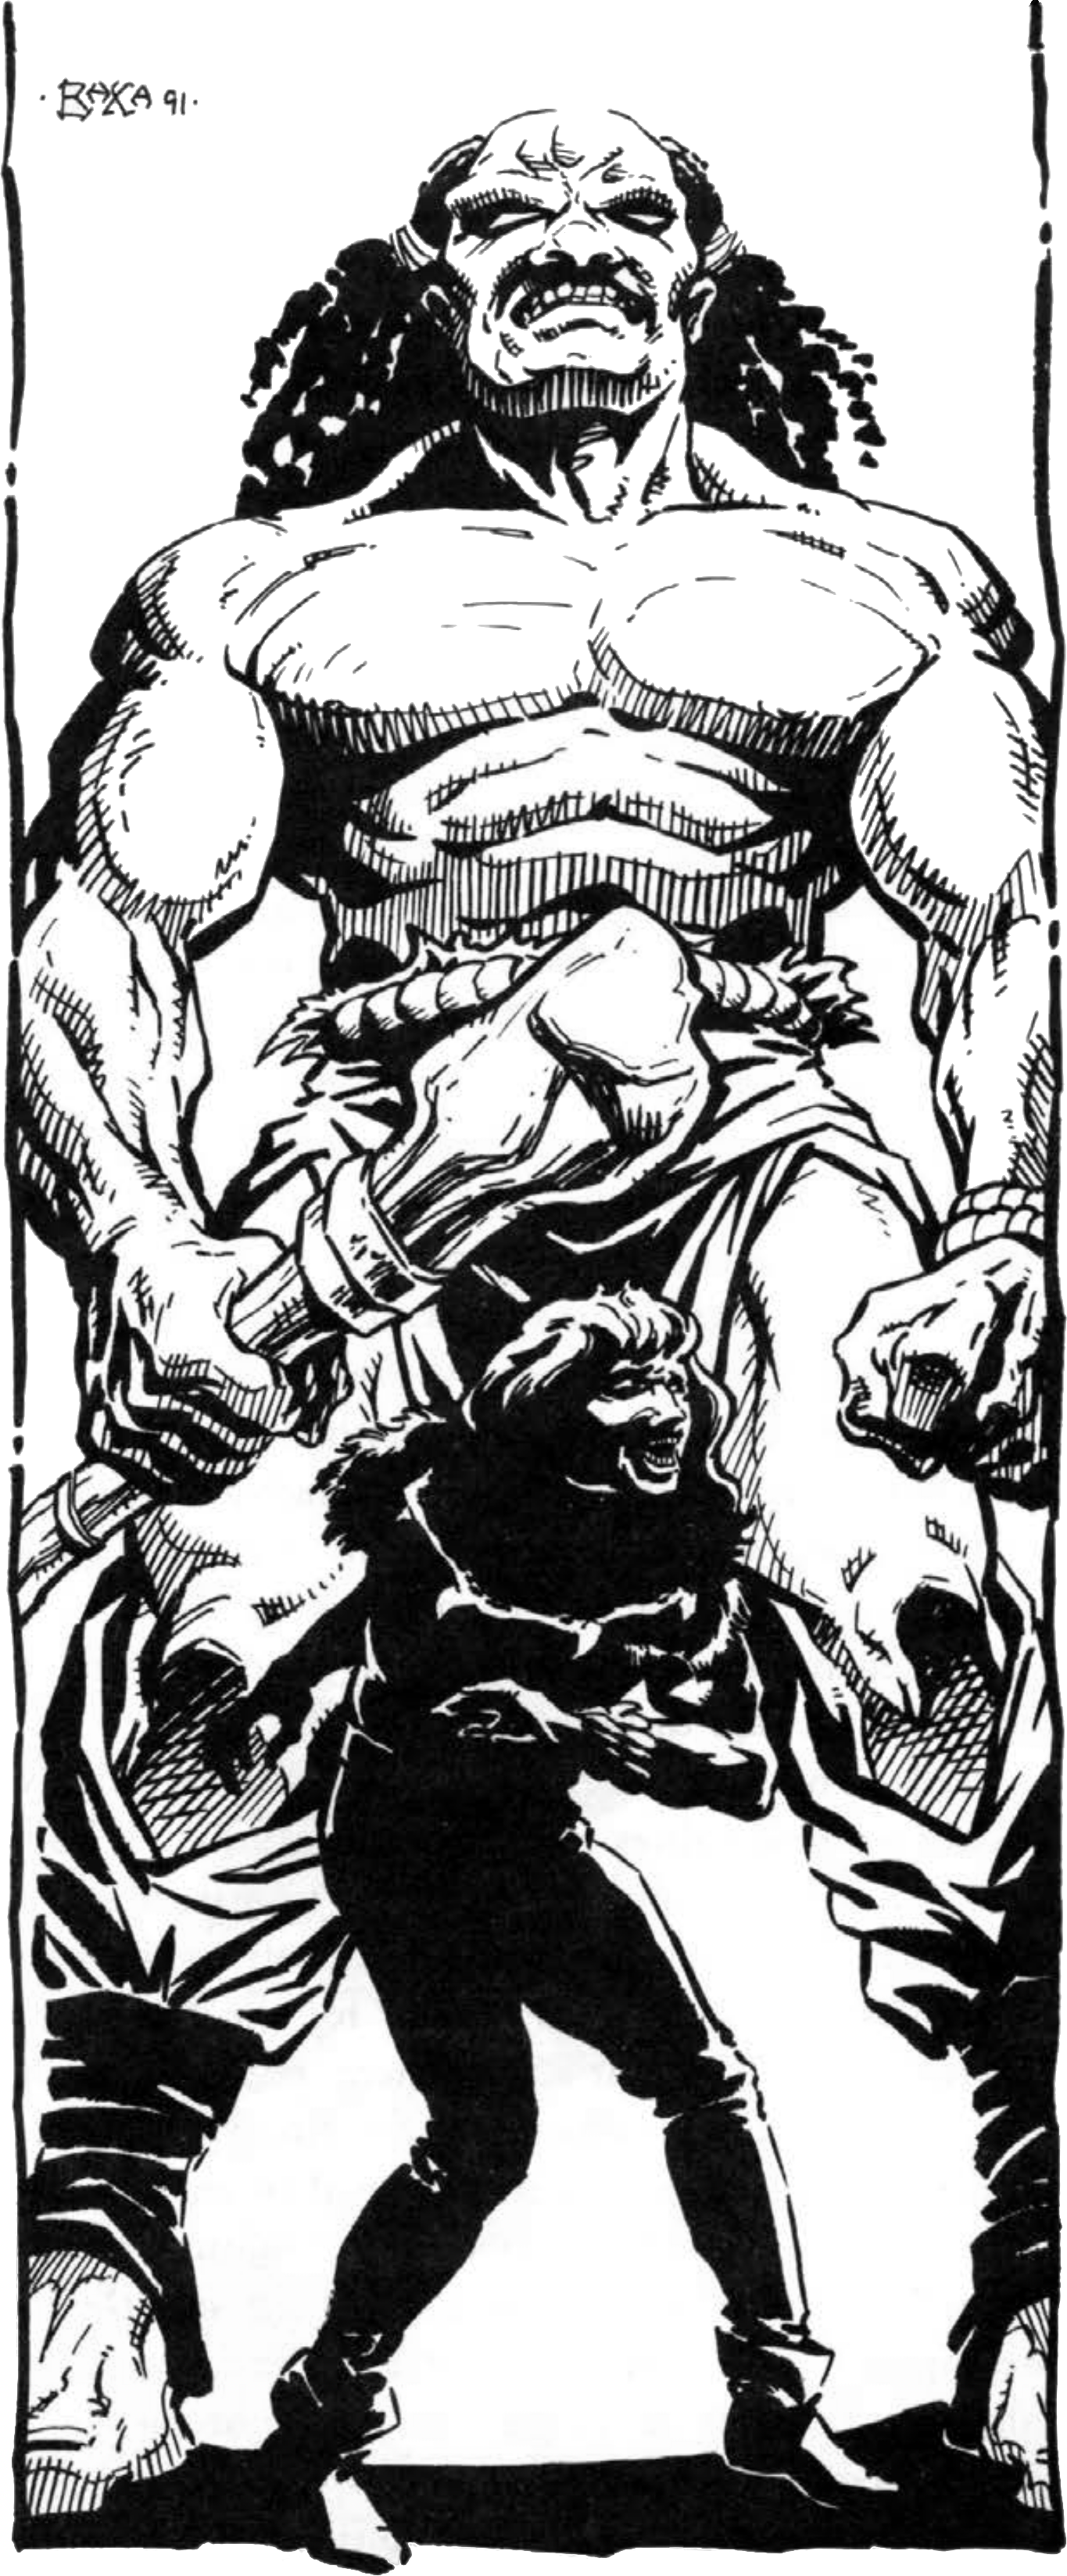
\includegraphics[width=\columnwidth]{images/halfgiant-1.png}
\WOTC
\end{figure}

\textbf{Personality:} Because of their artificial origins, there is no half-giant culture, tradition or homeland. Half-giants readily imitate the customs and cultures of their neighbors. Half-giants often display curiosity, a willingness to learn, and a general tendency towards kindness.

\textbf{Physical Description:} Physically, the half-giant is enormous, standing about 3.5 meters tall and weighing around 600 kg. Half-giants have thick hair, which is often kept braided (especially among females) or in a single tail that hangs behind the head and down the back. They dress in garb suitable to their occupation or environment. Half-giants mature at about 24 years of age and can live about 170 years.

\textbf{Relations:} The most powerful warriors on Athas, half-giants seem content to dwell in humanity's shadow. Half-giants tend to be friendly and eager to please, adopting the lifestyles, skills, and values of those they admire. A half-giant character who encounters a new situation looks around him to see what other people are doing. For example, a half-giant character that happens upon a Dwarven stone quarry may watch the dwarves, and then start quarrying stone himself. If he can make a living at it, he will continue to quarry stone just like his neighbor dwarves do; otherwise he will move on to something else.

\textbf{Alignment:} Half-giants can switch attitudes very quickly, taking on new values to fit new situations. A half-giant whose peaceful farming life is disrupted by marauders may soon adopt the morals of the renegades who sacked his village. A half-giant's nature is to switch his alignment aspect to imitate or otherwise react to a significant change around him.

\textbf{Half-Giant Lands:} Half-giants are most often found in the city-states, serving as gladiators, laborers, soldiers, and guards. A few half-giants collect into wilderness communities, often adopting the culture and customs of neighboring beings. The rare half-giant community often attaches itself to a charismatic or successful leader (not necessarily a half-giant) who demonstrates the tendencies they admire.

\textbf{Magic:} If a half-giant's companions accept wizardry, then the half-giant will also accept it. If a half-giant's companions hate wizardry, then the half-giant will be as eager as anyone to join in stoning a wizard. Among sophisticated companions who accept preserving magic but despise defiling magic, all but the brightest half-giants are likely to become confused, looking to their companions to see how they should react.

\textbf{Psionics:} While a single-classed half-giant psion is very rare, some half-giants take the path of the psychic warrior, becoming killing machines that can take apart a mekillot barehanded.

\textbf{Religion:} Half-giants do not display any affinity for the worship of one element over another.

\textbf{Language:} All half-giants speak the Common speech of slaves. Whatever tongue she speaks, the half-giant's voice is pitched so low as to occasionally be difficult to understand.

\textbf{Names:} Enslaved half-giants often have human names, and because of this they vary greatly. Free half-giants are likely to borrow the naming conventions of the race or people they are imitating at the time their child is born.

\textbf{Adventurers:} Half-giants are usually led to adventure by interesting companions of other races.

\subsection{Half-Giant Society}
A relatively young race, half-giants possess very little cultural identify of their own. Instead they adopt the customs and beliefs of those other cultures in which they live. Because of this, half-giants routinely change their alignment to match those around them who most influence them.
Half-giants can be found from one end of the Tablelands to the other, and often congregate in or near other population centers, absorbing the culture. Rarely do half-giants form communities of their own.

Unlike some other bastard races, half-giants can reproduce. A single off-spring is produced from half-giant unions after almost a year of pregnancy.

Though omnivorous, half-giants are tremendous consumers of water and food. They require twice the amount of food and water than humans. Clothing and equipment need twice the material to construct to fit a half-giant, leading to higher prices for half-giants.

Half-giants tend to damage objects and buildings around them through accidents of size alone. Some considerate half-giants camp outside city walls to avoid causing too much damage, but the draw of a city's culture and the below average intellect of most half-giants limits the number of half-giants who do so.

\subsection{Roleplaying Suggestions}
Always remember how much bigger and heavier you are than everyone else. Take advantage of your height in combat, but remember the disadvantages. Between your size and your lesser wits (even if you are a relatively intelligent half-giant people will assume you to be dull), you find yourself an object of comic relief. You are used to being teased and will endure more witty remarks than most people, but when you have been pushed too far your personality can suddenly shift, and you can unleash astonishing violence on your tormentors and any who stand in your way. Less frequently, these shifts can happen to you without provocation you just wake up with a different ethos and altered disposition.

Remember you are influenced by powerful personalities, and can shift your personality and ethics. You tend to imitate the tactics, clothes and demeanor of your ``little master.''
\subsection{Half-Giant Racial Traits}
\begin{itemize*}
    \item +8 Strength, +4 Constitution, $-2$ Dexterity, $-4$ Intelligence, $-4$ Wisdom, $-4$ Charisma: Half-giants are renowned for their great strength and dull wits.
    \item Large: As a Large creature, a half-giant takes a $-1$ penalty to Armor Class, a $-1$ penalty on attack rolls, and a $-4$ penalty on \skill{Hide} checks. She gains a +4 size bonus on grapple checks, and her lifting and carrying limits are double those of Medium characters, but she uses bigger weapons than humans use.
    \item Half-giants occupy a space of 3 meters and have a reach of 3 meters.
    \item Giant: Half-giants are creatures with the giant type.
    \item Half-giant base land speed is 12 meters.
    \item Darkvision: Half-giants can see in the dark out to 18 meters. Darkvision is black and white only, but it is otherwise like normal sight, and half-giants can function just fine with no light at all.
    \item Natural Armor: Half-giants have a +2 natural armor bonus to AC.
    \item Axis Alignment: One aspect of the half-giant's alignment must be fixed, and chosen during character creation. The other half must be chosen when they awake each morning. They are only bound to that alignment until they sleep again. For example, a half-giant may have a fixed lawful alignment. Every morning, he must choose to be lawful good, lawful neutral or lawful evil. This alignment change is not mandatory.
    \item Half-giants consume double the amount of food and water humans do.
    \item Favored Class: Barbarian. A multiclass half-giant's barbarian class does not count when determining whether he takes an experience point for multiclassing.
    \item Automatic Languages: Common. Bonus Languages: Dwarven, Gith, Giant. Half-giants will often pick up a race's tongue if imitating them long enough.
    \item Level Adjustment: +2. Half-giants are more powerful than the other races of the Tablelands and gain levels accordingly.
\end{itemize*}
\begin{figure*}[b!]
\centering
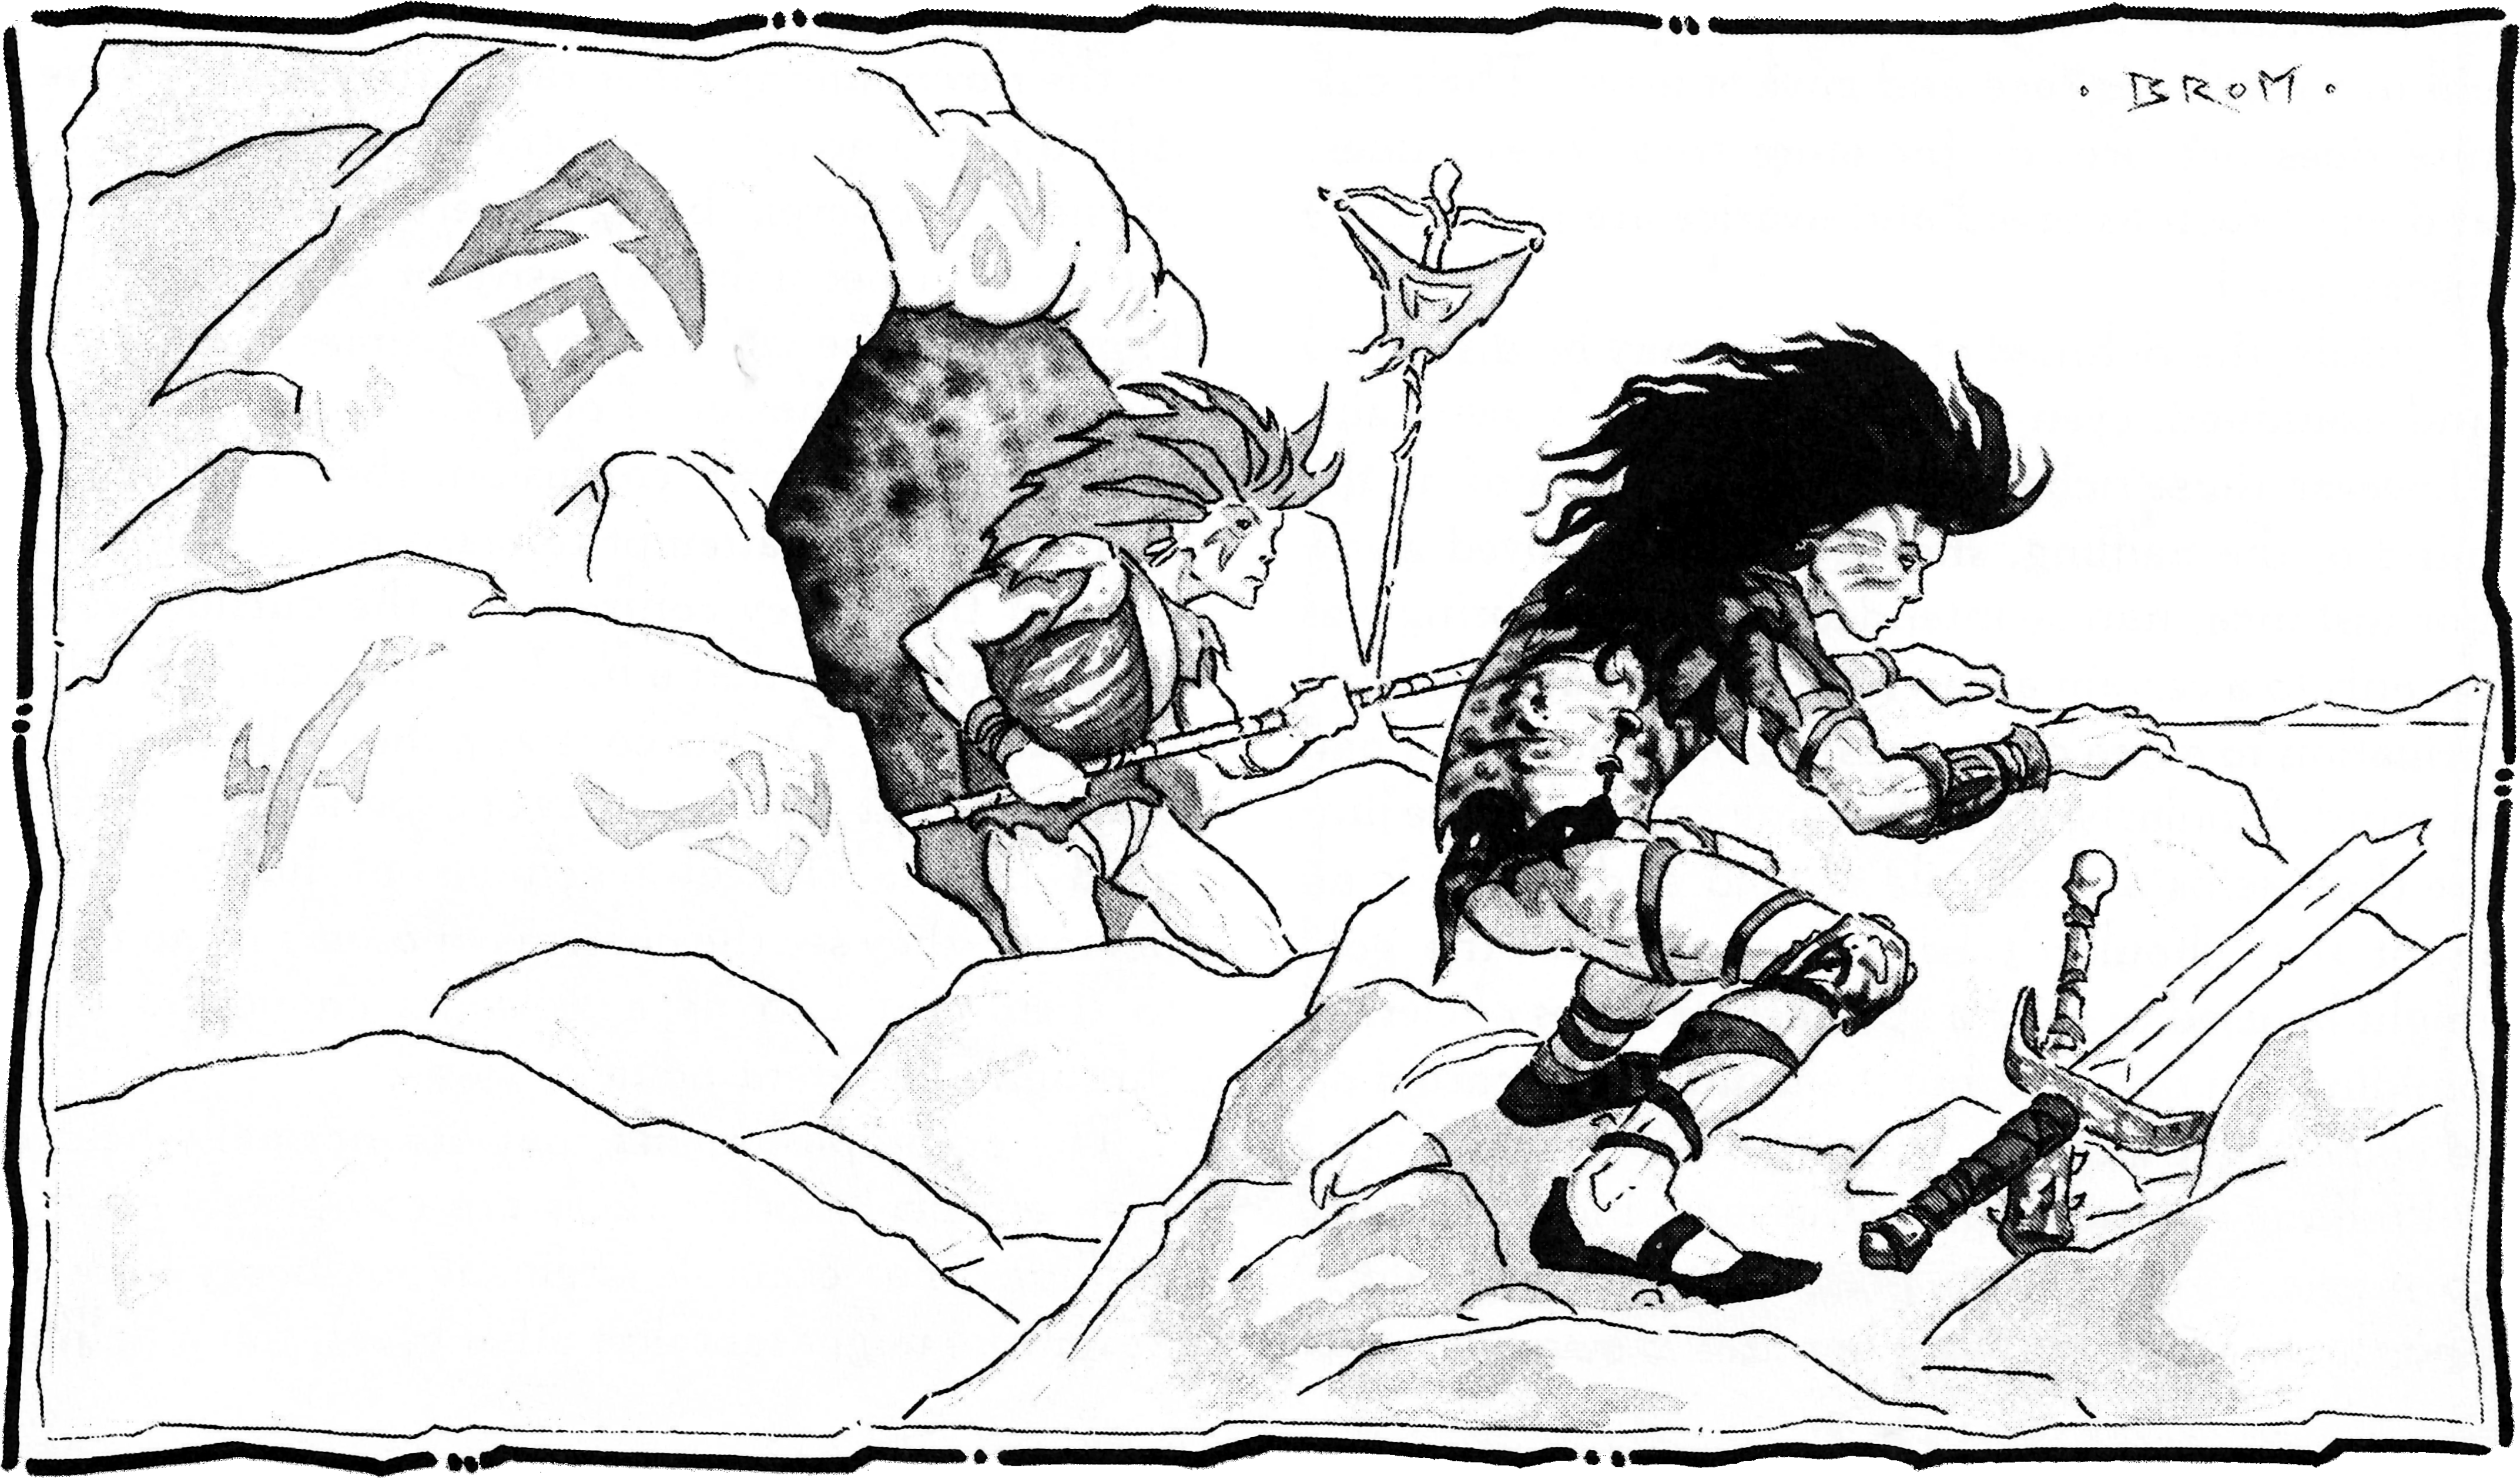
\includegraphics[width=\textwidth]{images/halfling-2.png}
\WOTC
\end{figure*}

\section{Halflings}
\Quote{Be wary of the forest ridge. The halflings who live there would as soon eat you alive as look at you. Chances are you won't even notice them until you've become the main course.}{Mo'rune, half-Elven ranger}

Halflings are masters of the jungles of the Ringing Mountains. They are small, quick and agile creatures steeped in an ancient and rich culture that goes back far into Athas' past. Although they are not common in the Tablelands, some halflings leave their homes in the forests to adventure under the{\tableheader Dark Sun}. As carnivores, halflings prefer to eat flesh raw.

\textbf{Personality:} Halflings have difficulty understanding others' customs or points of view, but curiosity helps some halflings overcome their xenophobia. Little concerned with material wealth, halflings are more concerned with how their actions will affect other halflings.

\textbf{Physical Description:} Halflings are small creatures, standing only about 1 meter tall and weighing 25 to 30 kilograms. Rarely affected by age, halfling faces are often mistaken for the faces of human children. They dress in loincloths, sometimes with a shirt or vest, and paint their skins with bright reds and greens. Forest halflings rarely tend to their hair, and some let it grow to great lengths, though it can be unkempt and dirty. They live to be about 120 years old.

\textbf{Relations:} Halfling's culture dominates their relations with others. They relate very well to each other, since they all have the same cultural traits and are able to understand each other. Halflings of different tribes still share a tradition of song, art and poetry, which serves as a basis of communication. Creatures that do not know these cultural expressions are often at a loss to understand the halfling's expressions, analogies and allusions to well-known halfling stories. Halflings can easily become frustrated with such ``uncultured'' creatures. They abhor slavery and most halflings will starve themselves rather than accept slavery.

\textbf{Alignment:} Halflings tend towards law and evil. Uncomfortable with change, halflings tend to rely on intangible constants, such as racial identity, family, clan ties and personal honor. On the other hand, halflings have little respect for the laws of the big people.

\textbf{Halfling Lands:} Halflings villages are rare in the tablelands. Most halflings live in tribes or clans in the Forest Ridge, or in the Rohorind forest west of Kurn. Many dwell in treetop villages. Non-halflings typically only see these villages from within a halfling cooking pot.

\textbf{Magic:} Many halfling tribes reject arcane magic. Tribes that accept wizards tend to have preserver chieftains. Only renegade halfling tribes are ever known to harbor defilers.

\textbf{Psionics:} Many halflings become seers or nomads. In the forest ridge, many tribal halflings become multiclassed seer/rangers, and become some of the deadliest trackers on Athas.

\textbf{Religion:} Halflings' bond with nature extends into most aspects of their culture. A shaman or witch doctor, who also acts as a spiritual leader, often rules their clans. This leader is obeyed without question. Halfling fighters willingly sacrifice themselves to obey their leader.

\textbf{Language:} Halflings rarely teach others their language, but some individuals of the Tablelands have learned the wild speech. Halflings found in the Tablelands often learn to speak Common.

\textbf{Names:} Halflings tend to have only one given name.

\textbf{Male Names:} Basha, Cerk, Derlan, Drassu, Entrok, Kakzim, Lokee, Nok, Pauk, Plool, Sala, Tanuka, Ukos, Zol.

\textbf{Female Names:} Alansa, Anezka, Dokala, Grelzen, Horga, Jikx, Joura, Nasaha, Vensa.

\textbf{Adventurers:} Exploring the Tablelands gives curious halflings the opportunity to learn other customs. Although they may at first have difficulty in understanding the numerous practices of the races of the Tablelands, their natural curiosity enables them to learn and interact with others. Other halflings may be criminals, renegades or other tribal outcasts, venturing into the Tablelands to escape persecution by other halflings.

\subsection{Halfling Society}
Most halflings have a common outlook on life that results in considerable racial unity across tribal and regional ties. Rarely will one halfling draw the blood of another even during extreme disagreements. Only renegade halflings do not share this racial unity, and are cast out of their tribes because of it.

Halfling society is difficult for other races to understand, as such concepts as conquest and plundering have no place. The most important value in halfling society is the abilities of the inner self as it harmonizes with the environment and the rest of the halfling race.

Halflings are extremely conscious of their environment. They are sickened by the ruined landscape of the Tyr region and desperately try to avoid having similar devastation occur to their homelands in the Forest Ridge. Most halflings believe that care must be taken to understand and respect nature and what it means to all life on Athas.

Halfling culture is expressed richly through art and song. Story telling in which oral history is passed on to the next generation is an important part of each halfling community. Halflings rely on this shared culture to express abstract thoughts and complicated concepts. This causes problems and frustration when dealing with non-halflings. Typically halflings assume that whomever they are talking to have the same cultural background to draw upon, and find it difficult to compensate for a listener who is not intimately familiar with the halfling history and ``lacks culture.''

Generally open-minded, wandering halflings are curious about outside societies and will attempt to learn all they can about other cultures. Never, will they adopt aspects of those cultures as their own, believing halfling culture to be innately superior to all others. Nor do they seek to change others' culture or views.

While halflings are omnivorous, they vastly prefer meat. Their meat heavy diet means that halflings view all living creatures, both humanoid and animal, as more food than equals. At the same time, most halflings believe that other races have the same perception of them. As a result, halflings are rarely likely to trust another member of any other race.

\subsection{Roleplaying Suggestions}
Remember to consistently take your height into account. Roleplay the halfling culture described above: eating opponents, treating fellow halflings with trust and kindness, suspicion of big people, and general lack of interest in money.

\subsection{Halfling Racial Traits}
\begin{itemize*}
    \item $-4$ Strength, +4 Dexterity, +4 Wisdom, $-2$ Charisma: Halflings are quick and stealthy, but weaker than humans.
    \item Humanoid (halfling): Halflings are humanoid creatures with the halfling subtype.
    \item Small: As a Small creature, a halfling gains a +1 size bonus to Armor Class, a +1 size bonus on attack rolls, and a +4 size bonus on \skill{Hide} checks, but she uses smaller weapons than humans use, and her lifting and carrying limits are three-quarters of those of a Medium character.%Halflings gain a +1 size bonus to Armor Class and a +1 size bonus on all attack rolls.
    \item Halfling base land speed is 6 meters.
    % \item Halflings receive a $-2$ penalty to all \skill{Diplomacy} skill checks when dealing with other races.
    \item +4 racial bonus on \skill{Climb} and \skill{Jump} checks: Halflings are agile.
    \item +2 racial bonus on saving throws against spells and spell-like effects.
    \item +1 racial attack bonus with a thrown weapon: javelins and slings are common weapons in feral halfling society, and many halflings are taught to throw at an early age.
    \item Halflings get advantage on \skill{Listen} checks---they have keen ears. Their senses of smell and taste are equally keen; they get advantage to all Wisdom checks that assess smell or taste.
    \item Halfings consume half the amount of food and water humans do.
    \item Automatic Languages: Halfling. Bonus Languages: Common, Dwarven, Elven, Gith, Kreen, Rhul-thaun, Sylvan, and Yuan-ti.
    \item Favored Class: Druid, Ranger, or Rogue. A halfling must choose between druid, ranger, or rogue as favored class. This choice cannot be changed. A multiclass halfling's chosen class does not count when determining whether he takes an experience point for multiclassing.
    \item Level Adjustment: +1.
\end{itemize*}
\section{Muls}
\Quote{See, the trick is to break their will. Not too much, mind you. Nobody wants to watch a docile gladiator, and muls are too expensive to waste as labor slaves. But, you don't want them trying to escape every other day. Would you like to tell the arena crowd that their favorite champion will not be appearing in today's match because he died trying to escape your pens?}{Gaal, Urikite arena trainer}

Born from the unlikely parentage of dwarves and humans, muls combine the height and adaptable nature of humans with the musculature and resilience of dwarves. Muls enjoy traits that are uniquely their own, such as their robust metabolism and almost inexhaustible capacity for work. The hybrid has disadvantages in a few areas as well: sterility, and the social repercussions of being created for a life of slavery. Humans and dwarves are not typically attracted to each other. The only reason that muls are so common in the Tablelands is because of their value as laborers and gladiators: slave-sellers force-breed humans and dwarves for profit. While mul-breeding practices are exorbitantly lucrative, they are often lethal to both the mother and the baby. Conception is difficult and impractical, often taking months to achieve. Even once conceived, the mul takes a full twelve months to carry to term; fatalities during this period are high. As likely as not, anxious overseers cut muls from the dying bodies of their mothers.

\textbf{Personality:} All gladiators who perform well in the arenas receive some degree of pampered treatment, but muls receive more pampering than others. Some mul gladiators even come to see slavery as an acceptable part of their lives. However, those that acquire a taste of freedom will fight for it. Stoic and dull to pain, muls are not easily intimidated by the lash. Masters are loath to slay or maim a mul who tries repeatedly to escape, although those who help the mul's escape will be tormented in order to punish the mul without damaging valuable property. Once a mul escapes or earns his freedom, slavery remains a dominant part of his life. Most muls are heavily marked with tattoos that mark his ownership, history, capabilities and disciplinary measures. Even untattooed muls are marked as a potential windfall for slavers: it is clearly cheaper to ``retrieve'' a mul who slavers can claim had run away, than to start from scratch in the breeding pits.

\begin{figure}[t!]
\centering
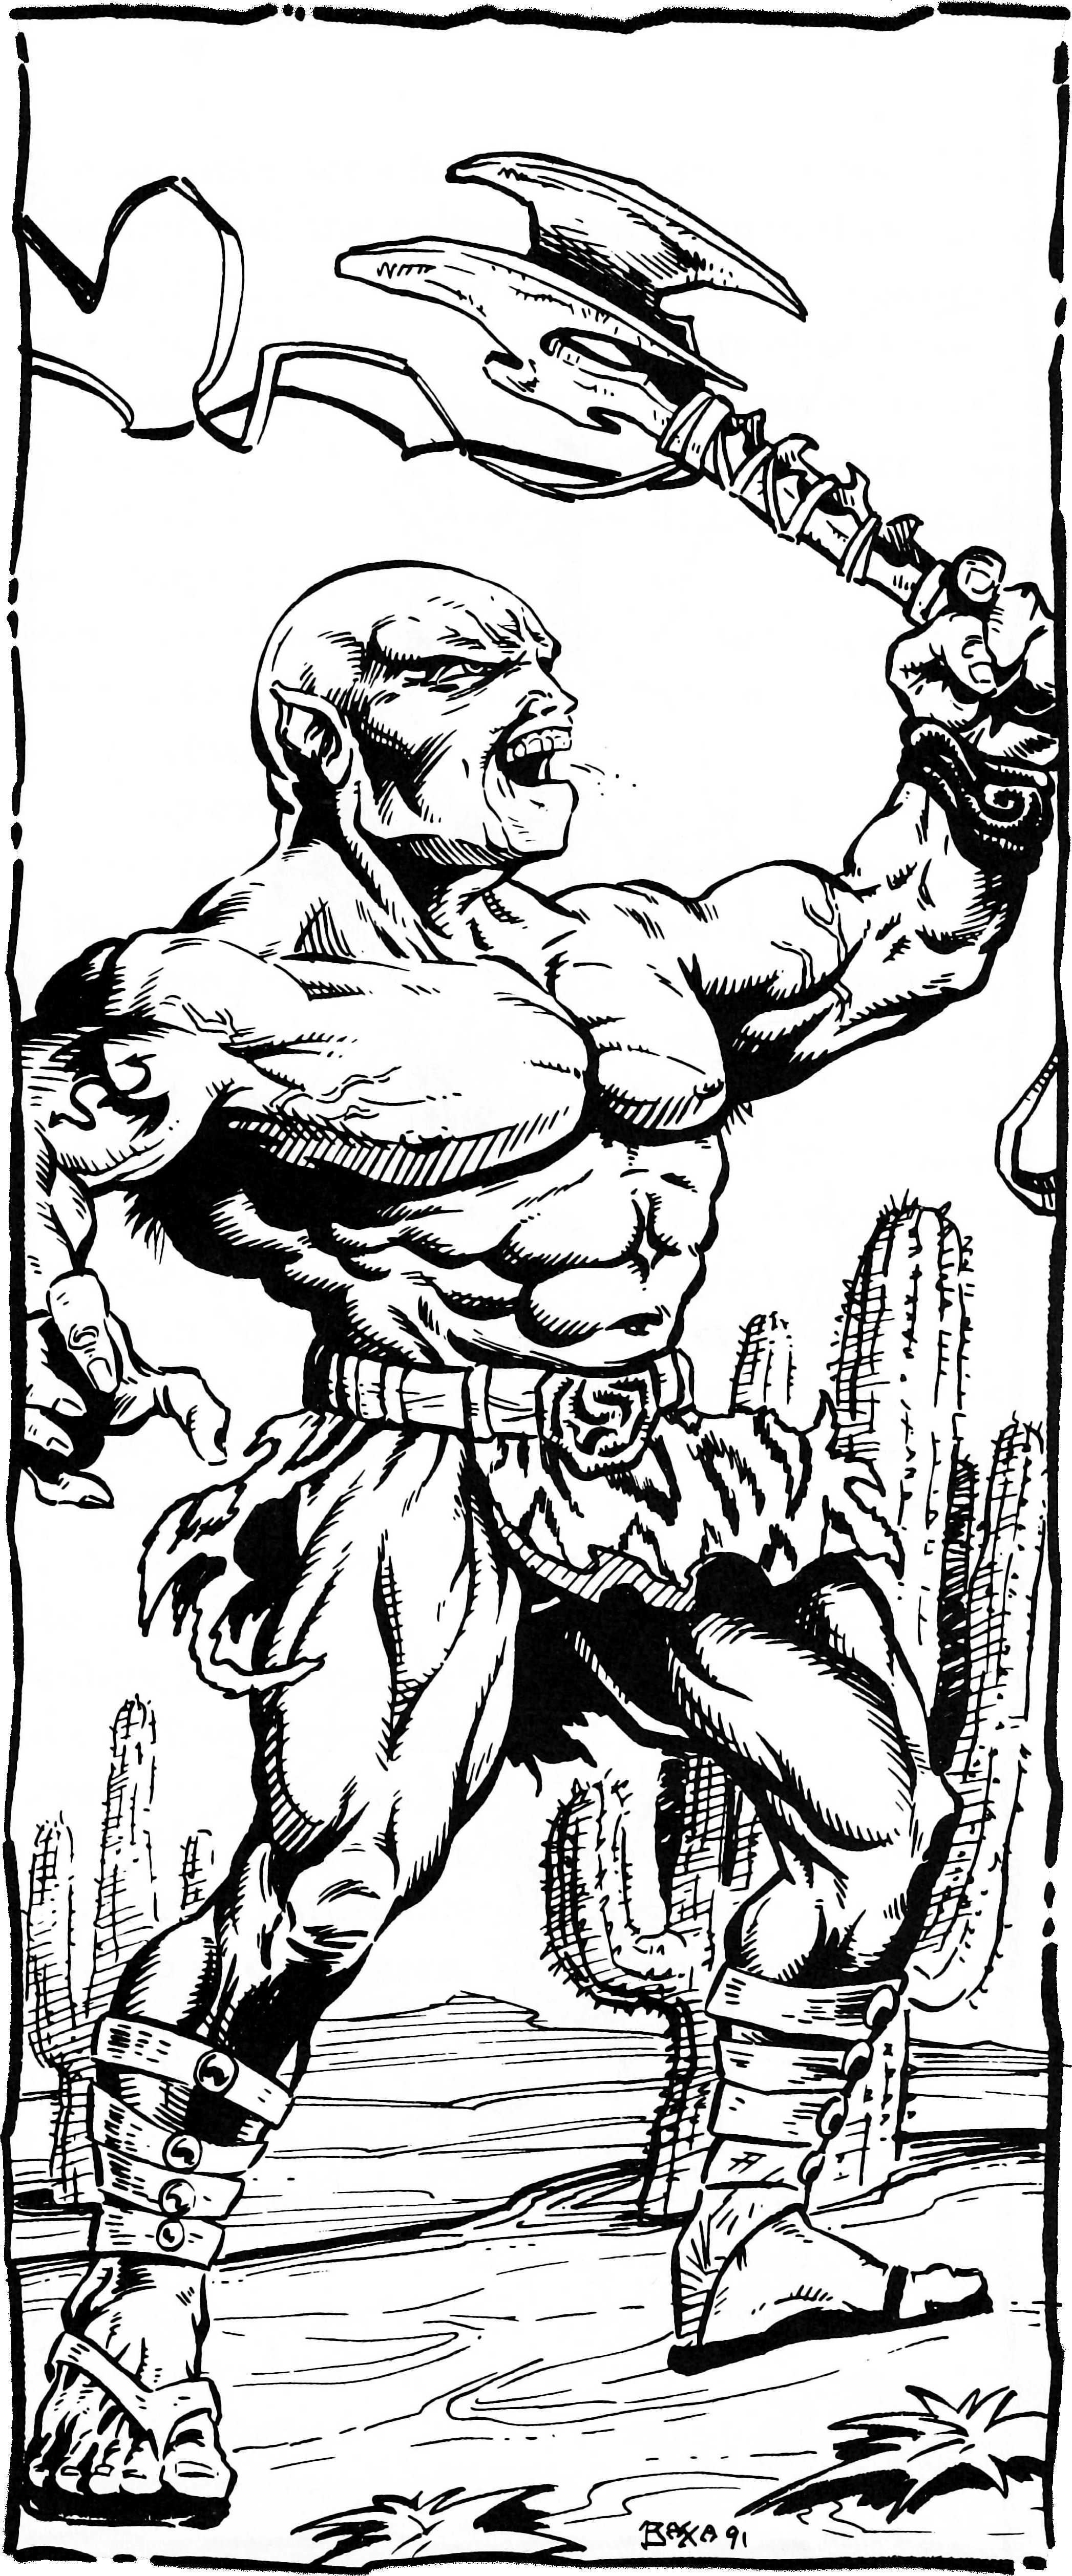
\includegraphics[width=\columnwidth]{images/mul-1.png}
\WOTC
\end{figure}

\textbf{Physical Description:} Second only to the half-giant, the mul is the strongest of the common humanoid races of the tablelands. Muls grow as high as 2.1 meters, weighing upwards of 125 kilograms, but carry almost no fat at all on their broad muscular frames. Universal mul characteristics include angular, almost protrusive eye ridges, and ears that point sharply backwards against the temples. Most muls have dark copper-colored skin and hairless bodies.

\textbf{Relations:} Most mul laborers master the conventions of slave life, figuring out through painful experience who can be trusted and who cannot. (Muls learn from their mistakes in the slave pits to a greater extent than other races not because they are cleverer, but because unlike slaves of other races they tend to survive their mistakes, while other slave races are less expensive and therefore disposable. Only the most foolish and disobedient mul would be killed. Most masters will sell a problem mul slave rather than kill him.) Their mastery of the rules of slave life and their boundless capacity for hard work allows them to gain favor with their masters and reputation among their fellow slaves.

\textbf{Alignment:} Muls tend towards neutrality with respect to good and evil, but run the gamut with respect to law or chaos. Many lawful muls adapt well to the indignities of slavery, playing the game for the comforts that they can win as valued slaves. A few ambitious lawful muls use the respect won from their fellow-slaves to organize rebellions and strike out for freedom. Chaotic muls, on the other hand, push their luck and their value as slaves to the breaking point, defying authority, holding little fear for the lash.

\textbf{Mul Lands:} As a collective group, muls have no lands to call their own. Occasionally, escaped muls band together as outlaws and fugitives, because of their common ex-slave backgrounds, and because their mul metabolism makes it easier for them to survive as fugitives while other races cannot keep up. Almost without exception, muls are born in the slave pits of the merchants and nobles of the city-states. Most are set to work as laborers, some as gladiators, and fewer yet as soldier-slaves. Very few earn their freedom, a greater number escape to freedom among the tribes of ex-slave that inhabit the wastes.

\textbf{Magic:} Muls dislike what they fear, and they fear wizards. They also resent that a wizard's power comes from without, with no seeming effort on the wizard's part, while the mul's power is born of pain and labor. Mul wizards are unheard of.

\textbf{Psionics:} Since most slave owners take steps to ensure that their property does not get schooled in the Way, it is rare for a mul to receive any formal training. Those that get this training tend to excel in psychometabolic powers.

\textbf{Religion:} Even if muls were to create a religion of their own, as sterile hybrids, they would have no posterity to pass it on to. Some cities accept muls as templars. Mul clerics tend to be drawn towards the strength of elemental earth.

\textbf{Language:} Muls speak the Common tongue of slaves, but those favored muls that stay in one city long enough before being sold to the next, sometimes pick up the city language. Because of their tireless metabolism, muls have the capacity to integrate with peoples that other races could not dream of living with, such as elves and Thri-kreen.

\textbf{Names:} Muls sold as laborers will have common slave names. Muls sold as gladiators will often be given more striking and exotic names. Draji names (such as Atlalak) are often popular for gladiators, because of the Draji reputation for violence. Masters who change their mul slaves' professions usually change their names as well, since it is considered bad form to have a gladiator with a farmer's name, and a dangerous incitement of slave rebellions to give a common laborer the name of a gladiator.

\textbf{Adventurers:} Player character muls are assumed to have already won their freedom. Most freed mul gladiators take advantage of their combat skills, working as soldiers or guards. Some turn to crime, adding rogue skills to their repertoire. A few muls follow other paths, such as psionics, templar orders or elemental priesthoods.

\subsection{Mul Society}
Muls have no racial history or a separate culture. They are sterile and cannot reproduce, preventing them from forming family groups and clans. The vast majority of muls are born in slavery, through breeding programs. Often the parents resent their roles in the breeding program and shun the child, leaving the mul to a lonely, hard existence. The taskmaster's whip takes the place of a family. For these reasons, many muls never seek friends or companionship, and often have rough personalities with tendencies towards violence.

The mul slave trade is very profitable, and thus the breeding programs continue. A slave trader can make as much on the sale of a mul as he could with a dozen humans. As slaves, a mul has his profession selected for him and is given extensive training as he grows.

Mul gladiators are often very successful, and win a lot of money for their owners. Highly successful gladiators are looked after by their owners, receiving a large retinue of other slaves to tend to their whims and needs. This has lead to the expression, ``pampered like a mul,'' being used often by the common folk.

Muls not trained as gladiators are often assigned to hard labor and other duties that can take advantage of the mul's hardy constitution and endurance.

\subsection{Roleplaying Suggestions}
Born to the slave pens, you never knew love or affection; the taskmaster's whip took the place of loving parents. As far as you have seen, all of life's problems that can be solved are solved by sheer brute force. You know to bow to force when you see it, especially the veiled force of wealth, power and privilege. The noble and templar may not look strong, but they can kill a man with a word. You tend towards gruffness. In the slave pits, you knew some muls that never sought friends or companionship, but lived in bitter, isolated servitude. You knew other muls who found friendship in an arena partner or co-worker. You are capable of affection, trust and friendship, but camaraderie is easier for you to understand and express - warriors slap each other on the shoulder after a victory, or give their lives for each other in battle. You don't think of that sort of event as ``friendship'' - it just happens.

\subsection{Mul Racial Traits}
\begin{itemize*}
    \item +4 Strength, +2 Constitution, $-2$ Intelligence, $-4$ Charisma: Combining the human height with the Dwarven musculature, muls end up stronger than either parent race, but their status as born-to-be slaves makes them insecure in their dealings with others.
    \item Humanoid (dwarf): Muls are humanoid creatures with the dwarf subtype.
    \item Medium: As Medium creatures, muls have no bonuses or penalties due to size.
    \item Mul base land speed is 9 meters.
    % \item Darkvision: Muls can see in the dark up to 9 meters. Darkvision is black and white only, but is otherwise like normal sight, and muls can function just fine with no light at all.
    \item Muls have +2 racial bonus on his damage rolls with light or thrown weapons (including unarmed strikes).
    \item Extended Activity: Muls require double the amount of time before making any check related to endurance.
    \begin{itemize*}
        \item Muls need to sleep every two days (but may choose to sleep every day);
        \item Muls can walk for 16 hours before beginning a forced march;
        \item Muls can hold their breath or run for a number of rounds equal to four times their Constitution score;
        \item Muls can go without food for six days;
        \item Muls can go without water for two days plus a number of hours equal to twice their Constitution score;
        \item Muls make Constitution checks every two hours of marching beyond 16 hours;
        \item Muls make Constitution checks every two rounds to continue holding their breath or running;
        \item Muls make Fortitude checks every two hours in a very hot (32 °C to 42 °C) or very cold ($-17$ °C to 4 °C) environments, every 20 minutes in severe heat (43 °C to 60 °C) or severe cold ($-28$ °C to $-18$ °C), and every 10 minutes in extreme heat \hskip10cm (61 °C to 82 °C), extreme cold ($-45$ °C to $-29$ °C), or worse environments;
        \item Muls make Constitution checks every two days after the first period without food;
        \item Muls make Constitution checks every two hours after the first period without water.
    \end{itemize*}
    % \item Tireless: Muls get a +4 racial bonus to checks for performing a physical action that extends over a period of time (running, swimming, holding breath, and so on). This bonus stacks with the \feat{Endurance} feat. This bonus may also be applied to savings throws against spells and magical effects that cause weakness, fatigue, exhaustion or enfeeblement.
    % \item Extended Activity: Muls may engage in up to 12 hours of hard labor or forced marching without suffering from the associated nonlethal damage and fatigue.
    \item Dwarven Blood: For all effects related to race, a mul is considered a dwarf. Muls, for example, are just as vulnerable to effects that affect dwarves as their dwarf ancestors are, and they can use magic items that are only usable by dwarves.
    % \item Nonlethal Damage Resistance 1/--. Muls are difficult to subdue, and do not notice minor bruises, scrapes, and other discomforts that pain creatures of other races.
    \item Favored Class: Fighter or Gladiator. A mul must choose between fighter or gladiator as favored class. This choice cannot be changed. A multiclass mul's chosen class does not count when determining whether he takes an experience point for multiclassing.
    \item Automatic Language: Common. Bonus Languages: Dwarven, Elven, Gith, and Giant.
    \item Level Adjustment: +1.
\end{itemize*}
\section{Pterrans}
\Quote{The people of the Tablelands know nothing of life. They choose no Path for themselves, and consume everything until they are dead.}{Keltruch, pterran ranger}

\begin{figure}[b!]
\centering
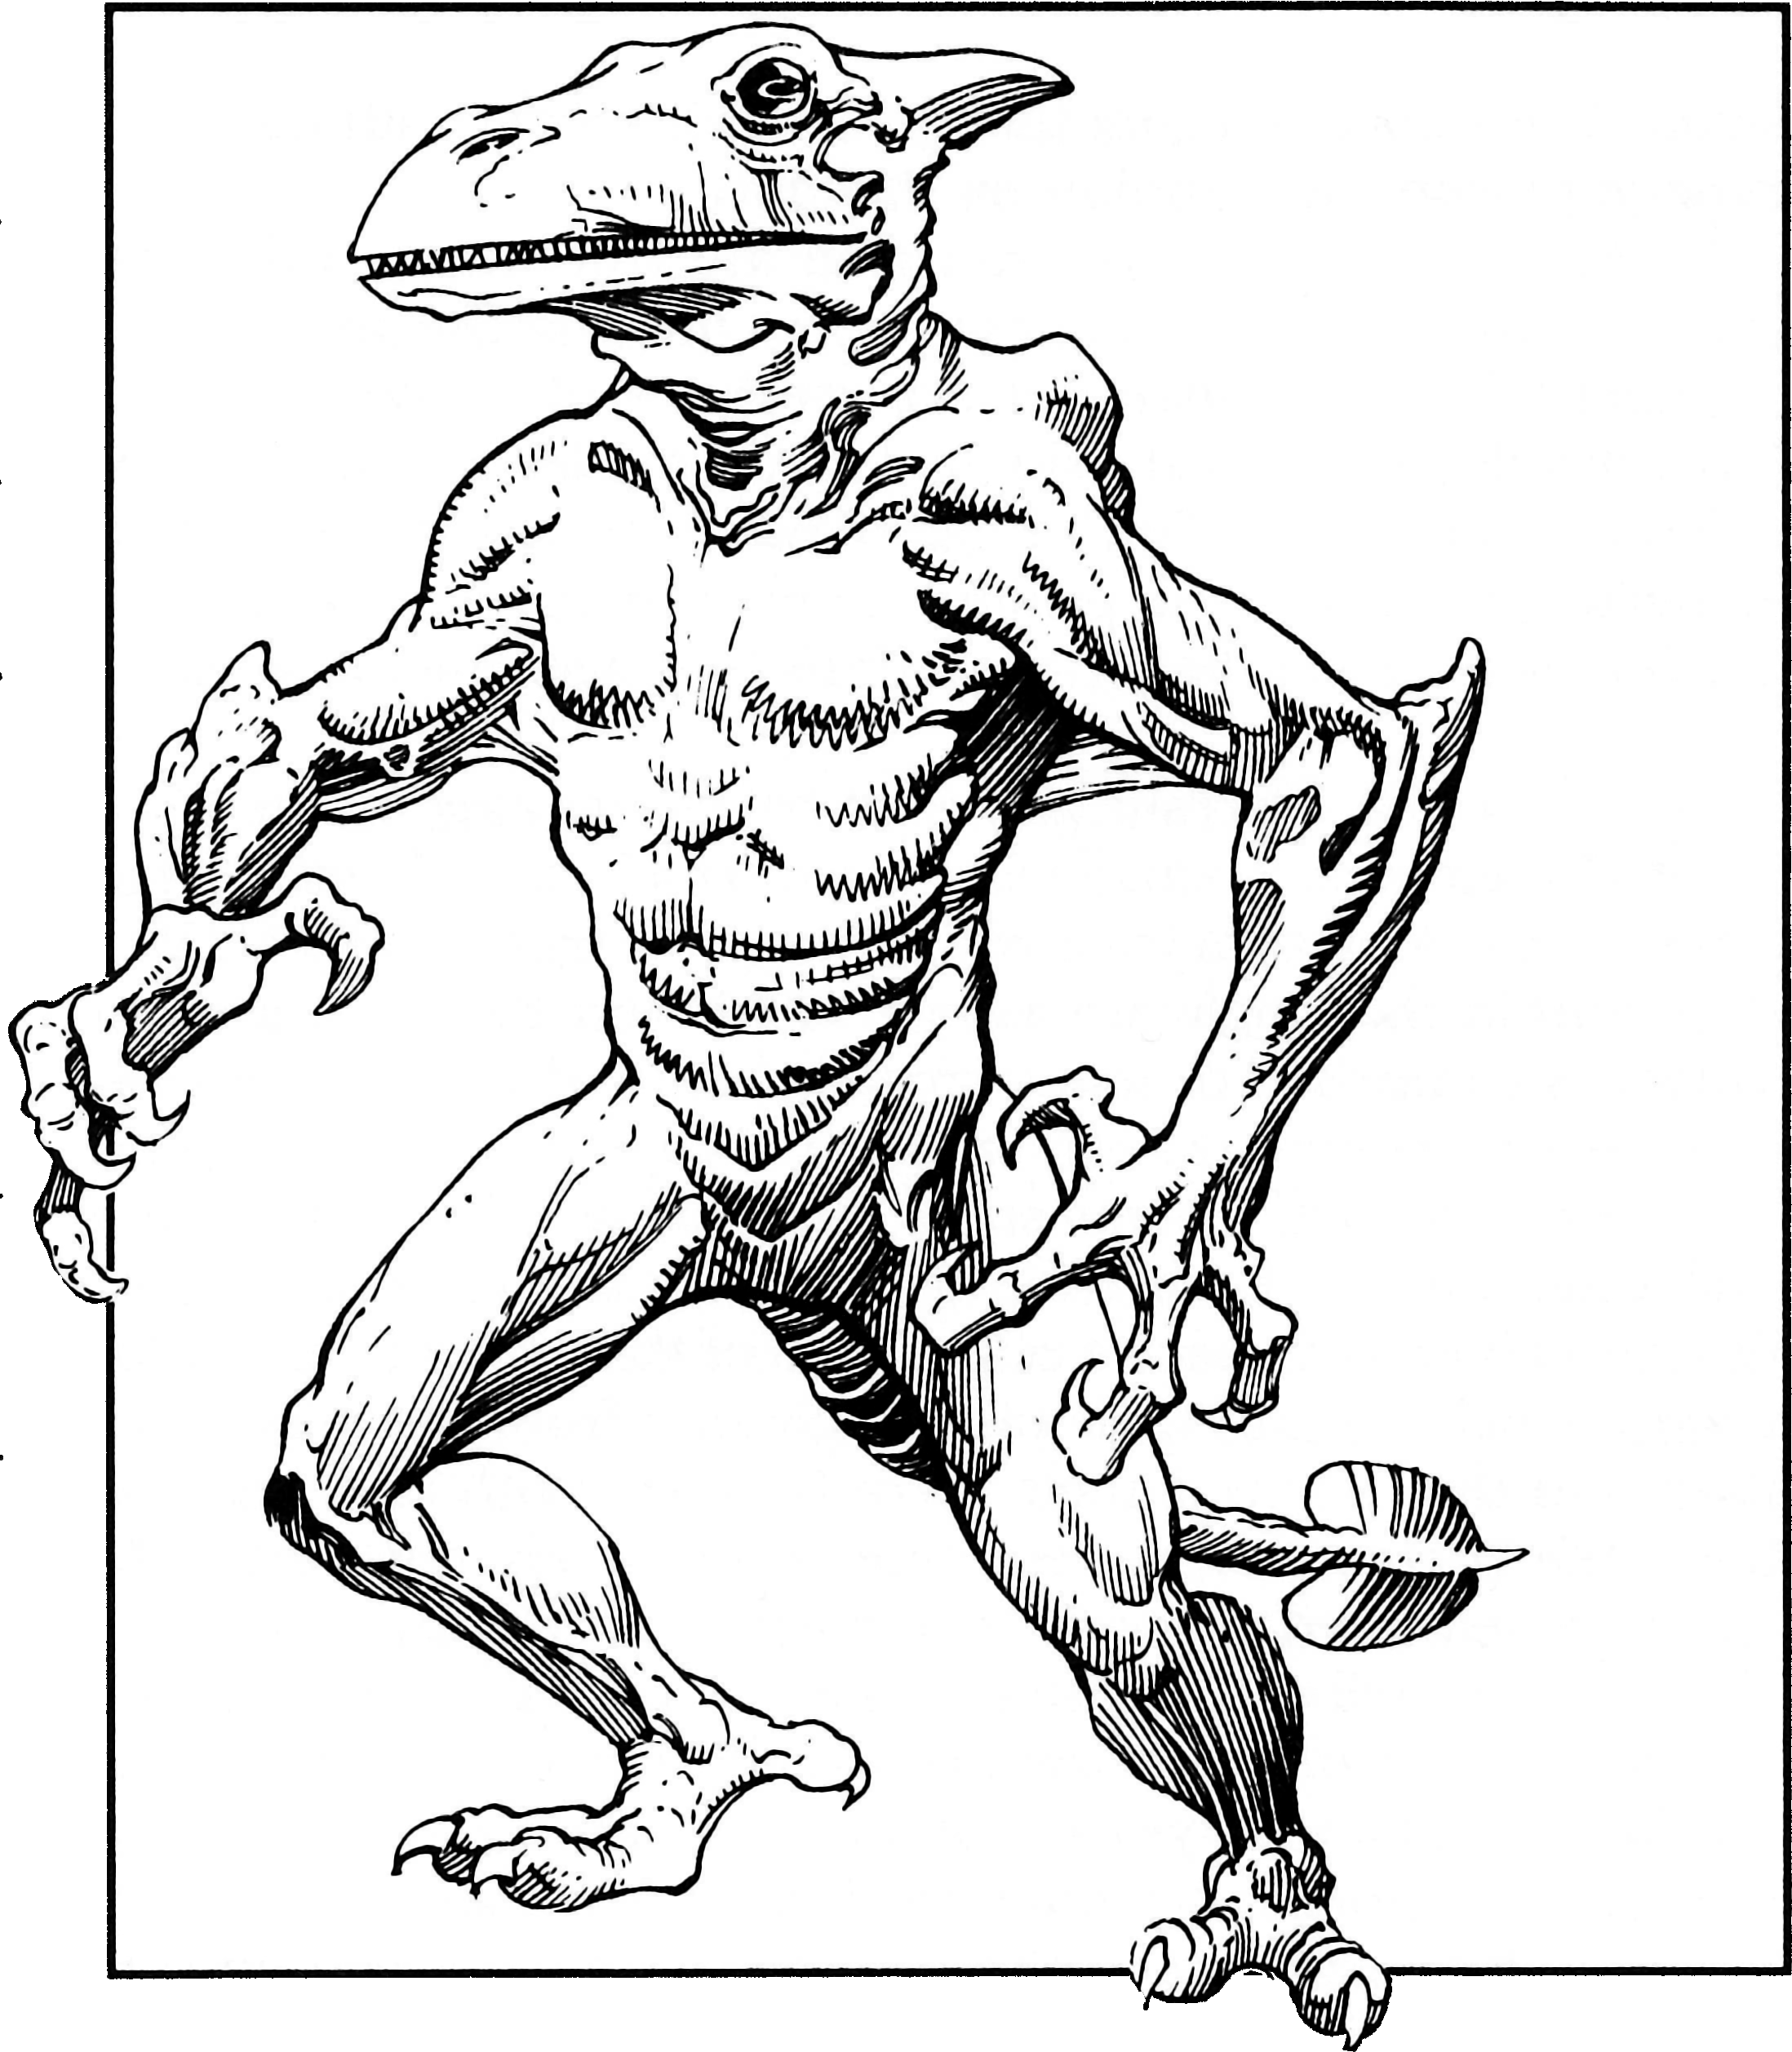
\includegraphics[width=\columnwidth]{images/pterran-1.png}
\end{figure}

Pterrans are rarely seen in the Tablelands. They live their lives in the Hinterlands, rarely leaving the safety of their villages. However, the recent earthquake and subsequent storms have brought disruption into the pterran's lives. More pterrans now venture outside their homes, and come to the Tyr region to seek trade and information.

\textbf{Personality:} Among strangers, pterrans seem like subdued, cautious beings, but once others earn a pterran's trust, they will find an individual that is open, friendly, inquisitive, and optimistic. In other respects, a pterran's personality is largely shaped by her chosen life path: Pterrans who choose the path of the warrior are less disturbed by the brutality of the Tablelands; they are constantly examining their surroundings and considering how the terrain where they are standing could be defended; they take greatest satisfaction from executing a combat strategy that results in victory without friendly casualties. Pterrans who choose the path of the druid are most interested in plants, animals, and the state of the land; they take greatest satisfaction when they eliminate a threat to nature. Pterrans that choose the path of the mind are most interested in befriending and understanding other individuals and societies; these telepaths take greatest satisfaction from intellectual accomplishments such as solving mysteries, exposing deception, resolving quarrels between individuals, and establishing trade routes between communities.

\textbf{Physical Description:} Pterrans are 1.5 to 1.9 meters tall reptiles with light brown scaly skin, sharp teeth, and a short tail. Pterrans wear little clothing, preferring belts and loincloths, or sashes. They walk upright, like humanoids, and have opposing thumbs and three-fingered, talon-clawed hands. Pterrans have two shoulder stumps, remnants of wings they possessed long ago, and a finlike growth juts out at the back of their heads. Pterrans weigh between 90 to 110 kilograms. There is no visible distinction between male and female pterrans.

\textbf{Relations:} Pterrans are new to the Tablelands, and unaccustomed to cultures and practices of the region. They have learned to not judge too quickly. Their faith in the Earth Mother means they undertake their adventure with open minds, but they will remain subdued and guarded around people they do not trust. A pterran's respect for the Earth Mother governs all his behavior. Creatures that openly destroy the land or show disrespect for the creatures of the wastes are regarded suspiciously. Pterrans understand the natural cycle of life and death, but have difficulty with some aspects of the city life, such as cramped living spaces, piled refuse, and the smells of unwashed humanoids.

\textbf{Alignment:} Pterrans tend towards lawful, well-structured lives, and most of them are good. Evil pterran adventurers are usually outcasts who have committed some horrible offense.

\textbf{Pterran Lands:} Most adventuring pterrans come from one of two villages in the Hinterlands, southwest of the Tyr regions: Pterran Vale and Lost Scale.

\textbf{Magic:} The wizard's use of the environment as a source of power conflicts with a pterran's religious beliefs. Pterrans will cautiously tolerate members of other races who practice preserving magic, if the difference is explained to them.

\textbf{Psionics:} Virtually all pterrans have a telepathic talent, and pterran psions are nearly universally telepaths. Telepathy is considered one of the honored pterran ``life paths.''

\textbf{Religion:} Pterrans worship the Earth Mother, a representation of the whole world of Athas. Their devotion to the Earth Mother is deeply rooted in all aspects of their culture, and it defines a pterran's behavior. All rituals and religious events are related to their worship of the Earth Mother. Religious events include festivals honoring hunts or protection from storms, with a priest presiding over the celebration. Most pterran priests are druids.

\textbf{Language:} Pterran speak Saurian with an accent that is difficult for other races to understand. The long appendage at the back of their head enables them to create sounds that no other race in the Tablelands can reproduce. The sounds are low, and resonate through the pterran's crest. Humanoid vocal chords cannot reproduce such sounds. Pterrans learn the Common tongue easily, but speak it with a slight, odd accent.

\textbf{Names:} Pterrans earn their first name just after they hatch, based on the weather and season of their hatching. After the pterran has decided upon a Life Path and has completed their apprenticeship, she receives title that becomes the first part of her name. This marks her transition into pterran society. There are a number of traditional names associated with each Life Path, but names do not always come from these ranks.

\textbf{Male Names:} Airson, Darksun, Earthsong, Suntail, Goldeye, Onesight, Terrorclaw.

\textbf{Female Names:} Cloudrider, Greenscale, Lifehearth, Rainkeeper, Spiritally, Watertender.

\textbf{Path Name:} Aandu, Caril, Dsar, Everin, Illik, Myril, Odten, Qwes, Pex, Ptellac, Ristu, Ssrui, Tilla, Xandu.

\textbf{Tribe or Village Names:} Pterran Vale, Lost Scale

\textbf{Adventurers:} Pterrans adventure because they believe the recent earthquake and disturbing events are signs from the Earth Mother that they should get more involved in the planet's affairs. They believe that these recent upheavals of nature are signs that the Earth Mother needs help, and this is a call the pterrans will gladly accept. As such, the most brave and adventurous of the pterrans have begun to establish contact with Tyr and some merchant houses, hoping to expand their contacts and information.

\subsection{Pterran Society}
Pterran society is based largely on ceremony and celebrations. An area is set aside in the center of each village for ceremonies. Pterrans revere the world of Athas as the Earth Mother, and believe themselves to be her favored children. Throughout the day, they engage in a number of ceremonies that give thanks to the Earth Mother. These are led by druids who play a very important role in pterran society.

A pterran village is a collection of many smaller family dwellings. Pterrans always bear young in pairs.

At age 15 every pterran chooses a ``life path.'' The three main life paths are the path of the warrior, the path of the druid and the path of the psionicist, though lesser life paths exist as well.

More pterrans follow the path of the warrior than any of the other paths, and become protectors of their villages as well as the tribe's weapon makers.

Pterrans that choose the path of the druid provide an important role in the daily ceremonies to the Earth Mother.

Fewer pterrans choose the path of the psionicist than the other two major paths, as psionics are viewed as outside of nature. Psionicists are viewed with suspicion by the rest of the tribe; however, they do provide valuable skills to the tribe and are often the tribe's negotiators when they meet outsiders.

Pterrans are omnivores. Much of their diet comes from hunting animals and raising crops. Kirre, id fiend, and flailer are all considered pterran delicacies.

\subsection{Roleplaying Suggestions}
Remember your character class is your ``life path.'' You think of yourself, and present yourself first and foremost as a druid, a warrior or a psion. Remember your daily celebrations and giving of thanks to the Earth Mother. You can usually find a reason to be grateful. Disrespect for the land angers you, since the whole land has withered under the disrespect of foolish humans and others. You celebrate with song and with dance. You have a good sense of humor but it does not extend to blasphemies such as defiling. In initial role-playing situations, you are unfamiliar with the customs and practices of the societies of the Tyr Region. However, you are not primitive by any definition of the word. You look upon differences with curiosity and a willingness to learn, as long as the custom doesn't harm the Earth Mother or her works.

\subsection{Pterran Racial Traits}
\begin{itemize*}
    \item $-2$ Dexterity, +2 Wisdom, +2 Charisma: Pterrans' strong confidence and keen instincts for others' motives make them keen diplomats, and when they take the path of the psion, powerful telepaths.
    \item Humanoid (psionic, reptilian): Pterrans are humanoid creatures with the psionic and reptilian subtypes.
    \item Medium: As Medium creatures, pterrans have no special bonuses or penalties due to size.
    \item Pterran base land speed is 9 meters.
    \item Poor Hearing: Pterrans have only slits for ears, and their hearing sense is diminished. Pterrans suffer a $-2$ penalty to Listen checks.
    \item Natural Weaponry: Pterrans can use their natural weapons instead of fighting with crafted weapons if they so choose. A pterran can rake with their primary claw attack for 1d3 of damage for each claw, and they bite for 1d4 points of damage as a secondary attack.
    \item Psi-Like Ability: At will---\psionic{missive}. All pterrans are gifted from the day they hatch with the ability to communicate telepathically, but only with their fellow reptiles. Manifester level is equal to \onehalf Hit Dice (minimum 1st).
    \item Weapon Familiarity: The following weapon is treated as martial rather than as an exotic weapon: thanak. This weapon is more common among pterrans than among other races.
    \item Automatic Languages: Saurian. Bonus Languages: Common, Dwarven, Elven, Halfling, Giant, Gith, Kreen, and Yuan-ti. Pterran know the languages of the few intelligent creatures that live in the Hinterlands.
    \item Life Path: A pterran's life path determines his favored class. Those following the Path of the Druid have druid as a favored class; the Path of the Mind gives psion as a favored class, while the Path of the Warrior gives ranger as a favored class. A Pterran chooses a life path upon coming of age, and the path cannot be changed once chosen at character creation time.
\end{itemize*}
\section{Thri-kreen}
\Quote{This one does not speak with the quivering soft shells that lay about all night. This one might eat you, but never speak.}{Tu'tochuk}

\Figure*{t}{images/thrikreen-1.png}

Thri-kreen are the strangest of the intelligent races of the Tablelands. These insectoid beings possess a mindset very different from any humanoid being encountered. They roam the wastes in packs, hunting for food day and night, since they require no sleep. Thri-kreen are quick and agile and make fearsome fighters, feared throughout the wastes.

\textbf{Personality:} Since thri-kreen (also known simply as the kreen) do not require sleep, they have difficulty understanding this need in the humanoid races. They have difficulty understanding this state of ``laziness'' in others. Other behaviors of humanoids seem unnecessarily complex. A keen's life is simple: hunt prey. Kreen live for the hunt, and own only what they can carry.

\textbf{Physical Description:} Mature thri-kreen stand about 2.1 meters tall, with a rough body length of 3.3 meters. Their four arms end in claws; their two legs are extremely powerful, capable of incredible leaps. However, kreen are unable to jump backwards. Their body is covered with a sandy-yellow chitin, a tough exoskeleton that grants the thri-kreen protection from blows. Their head is topped with two antennae, and their two eyes are compound and multifaceted. The kreen mouth consists of small pincers. Male and female thri-kreen are physically indistinguishable. Thri-kreen usually do not wear clothing, but wear some sort of harness to carry weapons and food. Many wear leg or armbands, or bracelets. Some attach rings on different places on their chitin, though this requires careful work by a skilled artisan.

\textbf{Relations:} The pack mentality dominates a keen's relation with others. Kreen hunt in packs, small groups that assemble together. Kreen will hunt prey in the same region for a while, but move on before their prey has been depleted. A kreen that joins a group of humanoids will often try to establish dominance in the group. This can be disconcerting to those unaware of the keen's behavior, since establishing dominance usually means making threatening gestures. Once the matter is settled, they will abide by the outcome. Thri-kreen view humanoids as sources of food, though they don't usually hunt them, only in dire need. Many kreen have a particularly fond taste for elves; as such, meetings between these two races are often tense. However, once part of a clutch, thri-kreen will never turn on their humanoid friends, even in the worst of situations.

\textbf{Alignment:} Most thri-kreen are lawful, since the pack mentality is ingrained in their beings. Kreen that deviate from this mentality are rare.

\textbf{Kreen Lands:} No thri-kreen settlements exist in the Tyr region; kreen encountered there are either small packs of kreen, or else adventuring with humanoids. To the north of the Tyr region, beyond the Jagged Cliffs, past the Misty Border, lies the Kreen Empire. This great nation of kreen rules the Crimson Savanna, forming great city-states that rival the humanoid city-states of the Tyr region.

\textbf{Magic:} Thri-kreen have no natural disposition towards magic, and a wizard's use of the environment as a source of power conflicts with a keen's beliefs. As well, the keen's lack of sleep and its instinctual need to hunt do not lend themselves well to magical study. Kreen wizards are extremely rare: no one has ever seen one in the Tablelands.

\textbf{Psionics:} Kreen view psionics as a natural part of their existence. Some packs rely on telepathy to communicate with each member and coordinate their hunting abilities. Many kreen also use psionic powers to augment their already formidable combat prowess. Psychometabolic powers are often used to boost speed, metabolism or strength to gain an advantage in combat. Most kreen (even non-adventurers) take the psychic warrior class, which kreen consider a natural part of growing up. Kreen do not need instruction to advance in the psychic warrior class---it comes to them as part of their ancestral memory.

\textbf{Religion:} Thri-kreen have no devotion to any god, but they hold nature and the elements in high regard. Ancestral memories guide them through their lives. Thri-kreen revere the Great One, a legendary kreen leader from the past.

\textbf{Language:} The Kreen language is very different from those of the other intelligent races. They have no lips or tongues, and so cannot make the same sounds humanoids make. Kreen language is made up of clicks, pops, or grinding noises.

\textbf{Names:} Kachka, Ka'Cha, Ka'Ka'Kyl, Klik-Chaka'da, Sa'Relka, T'Chai

\textbf{Adventurers:} Kreen adventure for different reasons. Most enjoy challenges presented by new prey. Some seek out the challenge of leading new clutches, new companions and observing the different ``hunting'' techniques of the dra (sentient meat-creatures such as humans).

\subsection{Thri-Kreen Society}
Thri-kreen hatch from eggs. All those who hatch at the same time form what is called a clutch. Thri-kreen gather in packs that roam the wastes. Each pack consists of several clutches that roam over an area that the pack considers theirs to hunt on. There are no permanent thri-kreen communities.

Clutches and packs are organized along strict order of dominance. The toughest member is leader; the second most powerful is second in command and so forth. A thri-kreen can challenge a superior for dominance initiating a contest. The contestants fight until one surrenders or dies. Afterwards, the matter is considered settled and there are no lingering resentments between victor and loser. The pack-mates take the view that the challenger was only acting to strength the pack.

Thri-kreen are obsessed with hunting. They are carnivores, but seldom hunt intelligent life for food. They do have a taste for elf, which gives them a bad reputation amongst Elven tribes. When not hunting, they craft weapons, teach their young, and craft sculptures.

The pack mentality is so ingrained in the culture that thri-kreen apply it to every situation. Thri-kreen feel compelled to be part of a clutch and will accept members of other races as clutch-mates.

\subsection{Roleplaying Suggestions}
You tend to rely on your natural attacks and special kreen weapons. Everything you kill is a potential dinner. You have a strong need for a party leader---obedience to this leader in the party is important to you. If you seem to be the most powerful and capable, then you will assume leadership; if someone challenges your authority then you will wish to test whether they are in fact stronger than you. It is not a question of vanity; you won't want to fight to the death, but merely to ascertain who is worthy to lead the party. You do not have the focus of a dwarf to complete a project, but you would give your life to protect your companions. If you did not trust and honor them as your own family, then you would not travel with them and work together with them. You do not understand the concept of sleep. It disturbs you that your dra companions lie unconscious for a third of their lifetimes. You own only what you can carry, caring little for money or other items that other races consider as treasure. Your philosophy of ownership sometimes leads you into conflict with presumptuous dra who think they can own buildings, land, and even whole herds of cattle!


% \Figure*{t}{images/adventurer-2.png}


\subsection{Thri-Kreen Racial Traits}
\begin{itemize*}
    \item +4 Dexterity, $-2$ Intelligence, +2 Wisdom, $-4$ Charisma: Thri-kreen are fast, but their alien mindset makes it difficult for them to relate to humanoids; furthermore, their ``clutch-mind'' instincts leave them with a poor sense of themselves as individuals.
    \item Monstrous Humanoid: Thri-kreen are not subject to spells or effects that affect humanoids only, such as \spell{charm person} or \spell{dominate person}.
    \item Medium: Thri-kreen receive no advantages or penalties due to size.
    \item Thri-kreen base land speed is 12 meters.
    \item Low-light Vision: Thri-kreen can see twice as far as a human in moonlight and similar conditions of poor illumination, retaining the ability to distinguish color and detail.
    \item Vestigial Antennae: Thri-kreen lessen miss chance from any type of concealment by 5\% (including total concealment or blindness). Thri-kreen have 15\% miss chance against foes with concealment, and 45\% miss chance against enemies with total concealment or when the thri-kreen is blinded.
    \item Sleep Immunity: Thri-kreen do not sleep, and are immune to sleep spells and similar effects. Thri-kreen spellcasters and manifesters still require 8 hours of rest before preparing spells or regaining power points.
    \item Water Efficient: Thri-kreen can go for one week on the amount of water a human needs in a day.
    \item Natural Armor: Thri-kreen have a +2 natural armor bonus to AC due to their naturally tough and resistant chitin.
    \item Multiple Limbs: Thri-kreen have four arms, and thus can take the \feat{Multiweapon Fighting} feat instead of the \feat{Two-Weapon Fighting} feat. Thri-kreen can also take the \feat{Multiattack} feat. (These are not bonus feats.)
    \item Natural Weapons: Thri-kreen may make bite and claw attacks as a full round action. Their primary claw attack does 1d4 points of damage for each of their four claws. Their secondary bite attack, deals 1d4 points of damage, and has a chance to poison. A thri-kreen can attack with a weapon (or multiple weapons) at its normal attack bonus, and make either a bite or claw attack as a secondary attack.
    \item Deflect Arrows: Thri-kreen gain the benefit of the \feat{Deflect Arrows} feat.
    \item Leap (Ex): When a thri-kreen reaches 3 Hit Dice, they become natural jumpers, gaining a +30 racial bonus to all \skill{Jump} checks.
    \item Poison (Ex): When a thri-kreen reaches 5 Hit Dice, their glands become able to deliver poison with a successful bite attack. Fortitude DC 11 + Con modifier. The initial and secondary damages are paralysis for 1d10 rounds.
    \item Weapon Familiarity: To thri-kreen, the chatkcha and gythka are treated as martial rather than exotic weapons. These weapons are more common among thri-kreen than among other races.
    \item Thri kreen have a +4 racial bonus on \skill{Hide} checks in sandy or arid areas.
    \item Alien Mind (Ex): A thri-kreen has difficulty understanding how the humanoid minds work. Whenever a thri-kreen targets a creature of another race with mind-affecting abilities, that creature gains +1 to its save against those powers.
    \item Automatic Languages: Kreen. Bonus Languages: Common, Dwarven, Elven, Entomic, Saurian, and Terran.
    \item Favored Class: Druid or Fighter. A thri-kreen must choose between druid or fighter as favored class. This choice cannot be changed. A multiclass thri-kreen's chosen class does not count when determining whether he takes an experience point for multiclassing.
    \item Level Adjustment: +1.
\end{itemize*}


\section{Other Races}
Athas is a place where members of different races are usually found in the same city-state, usually because they are going to be used in gladiatorial games as an exotic attraction, or to become slaves due to their physical might. Even though they are not usually concentrated on a specific area, these races are significant players in the Tablelands. It is only fitting then, that belgoi, gith, jozhals, ssurrans, tareks, taris, yuan-tis, and a variety of other creatures commonly viewed as monsters might appear as player characters in a {\tableheader Dark Sun} campaign. Cultural information about several monstrous races appears in \hyperref[chapter:Life on Athar]{Life on Athas}.
\Chapter{Description}
{In my travels I have found that Athas is a world of clashing cultures. Primitive hunters stalk their prey into a city's barley fields, and are in turn hunted down by outraged nobles. Nomadic herders clog the trading roads with their unruly flocks, slowing even the fastest merchant caravan to a crawl. To keep from being massacred in their sleep, villagers working the mines of the Ringing Mountains buy off feral halfling tribes with worthless glass baubles.

On Athas, there are as many different societies as there are groups of people. Each has found a different key to survival in this harsh world. Sometimes these different bands coexist peacefully; more often, they clash whenever they meet.

Surprisingly, all of these societies are shaped by the same four forces: barrenness, shortage of metal, psionics, and magic. If you understand how any society deals with these forces, you will understand the society itself.}
{The Wanderer's Journal}

\section{Alignment}
A creature's general moral and personal attitudes are represented by its alignment: lawful good, neutral good, chaotic good, lawful neutral, neutral, chaotic neutral, lawful evil, neutral evil, or chaotic evil.

Alignment is a tool for developing your character's identity. It is not a straitjacket for restricting your character. Each alignment represents a broad range of personality types or personal philosophies, so two characters of the same alignment can still be quite different from each other. In addition, few people are completely consistent.

\subsection{Typical Alignments}
Sentient creatures usually can be of any alignment, but as a group they have a typical or most common alignment. The table \tabref{Creature, Race, and Class Alignments} shows the alignments for the most common races, classes and creature in Athas. Creatures shown in \emph{italic} are always of the given alignment.

\Table{Creature, Race, and Class Alignments}{X X X}{
  \vskip2pt \tableheader Lawful Good
& \vskip2pt \tableheader Neutral Good
& \vskip2pt \tableheader Chaotic Good\\

Dwarves  & \emph{Aviarag} & \emph{Djinn} \\
Pterrans & Aarakocras     & Preservers \\
         &                & Rangers \\

  \vskip2pt \tableheader Lawful Neutral
& \vskip2pt \tableheader Neutral
& \vskip2pt \tableheader Chaotic Neutral \\
Drays      & \emph{Animals}    & Elves \\
Halflings  & \emph{Elementals} & Barbarians \\
Jozhal     & Humans            & Bards \\
Thri-kreen & Druids            & Gladiators \\
Villichi   & Psions            & Rogues \\

  \vskip2pt \tableheader Lawful Evil
& \vskip2pt \tableheader Neutral Evil
& \vskip2pt \tableheader Chaotic Evil \\
\emph{Efreet} & Anakore  & \emph{Shadows} \\
Belgoi        & Braxats  & \emph{Tembos} \\
Templars      & Giants   & Gith \\
              & Hej-kin  & Defilers \\
              & T'Chowbs & Scrabs \\
}

\subsection{Good vs. Evil}
Good characters and creatures protect innocent life. Evil characters and creatures debase or destroy innocent life, whether for fun or profit.

``Good'' implies altruism, respect for life, and a concern for the dignity of sentient beings. Good characters make personal sacrifices to help others.

``Evil'' implies hurting, oppressing, and killing others. Some evil creatures simply have no compassion for others and kill without qualms if doing so is convenient. Others actively pursue evil, killing for sport or out of duty to some evil deity or master.

People who are neutral with respect to good and evil have compunctions against killing the innocent but lack the commitment to make sacrifices to protect or help others. Neutral people are committed to others by personal relationships.

Being good or evil can be a conscious choice. For most people, though, being good or evil is an attitude that one recognizes but does not choose. Being neutral on the good-evil axis usually represents a lack of commitment one way or the other, but for some it represents a positive commitment to a balanced view. While acknowledging that good and evil are objective states, not just opinions, these folk maintain that a balance between the two is the proper place for people, or at least for them.

Animals and other creatures incapable of moral action are neutral rather than good or evil. Even deadly vipers and tigers that eat people are neutral because they lack the capacity for morally right or wrong behavior.

\subsection{Law vs. Chaos}
Lawful characters tell the truth, keep their word, respect authority, honor tradition, and judge those who fall short of their duties.

Chaotic characters follow their consciences, resent being told what to do, favor new ideas over tradition, and do what they promise if they feel like it.

``Law'' implies honor, trustworthiness, obedience to authority, and reliability. On the downside, lawfulness can include close-mindedness, reactionary adherence to tradition, judgmentalness, and a lack of adaptability. Those who consciously promote lawfulness say that only lawful behavior creates a society in which people can depend on each other and make the right decisions in full confidence that others will act as they should.

``Chaos'' implies freedom, adaptability, and flexibility. On the downside, chaos can include recklessness, resentment toward legitimate authority, arbitrary actions, and irresponsibility. Those who promote chaotic behavior say that only unfettered personal freedom allows people to express themselves fully and lets society benefit from the potential that its individuals have within them.

Someone who is neutral with respect to law and chaos has a normal respect for authority and feels neither a compulsion to obey nor a compulsion to rebel. She is honest but can be tempted into lying or deceiving others.

Devotion to law or chaos may be a conscious choice, but more often it is a personality trait that is recognized rather than being chosen. Neutrality on the lawful-chaotic axis is usually simply a middle state, a state of not feeling compelled toward one side or the other. Some few such neutrals, however, espouse neutrality as superior to law or chaos, regarding each as an extreme with its own blind spots and drawbacks.

Animals and other creatures incapable of moral action are neutral. Dogs may be obedient and cats free-spirited, but they do not have the moral capacity to be truly lawful or chaotic.

\subsection{The Nine Alignments}
Nine distinct alignments define all the possible combinations of the lawful-chaotic axis with the good-evil axis. Each alignment description below depicts a typical character of that alignment. Remember that individuals vary from this norm, and that a given character may act more or less in accord with his or her alignment from day to day. Use these descriptions as guidelines, not as scripts.

The first six alignments, lawful good through chaotic neutral, are the standard alignments for player characters. The three evil alignments are for monsters and villains.

\textbf{Lawful Good, ``Crusader'':} A lawful good character acts as a good person is expected or required to act. She combines a commitment to oppose evil with the discipline to fight relentlessly. She tells the truth, keeps her word, helps those in need, and speaks out against injustice. A lawful good character hates to see the guilty go unpunished.

Lawful good is the best alignment you can be because it combines honor and compassion.

\textbf{Neutral Good, ``Benefactor'':} A neutral good character does the best that a good person can do. He is devoted to helping others. He works with kings and magistrates but does not feel beholden to them.

Neutral good is the best alignment you can be because it means doing what is good without bias for or against order.

\textbf{Chaotic Good, ``Rebel'':} A chaotic good character acts as his conscience directs him with little regard for what others expect of him. He makes his own way, but he's kind and benevolent. He believes in goodness and right but has little use for laws and regulations. He hates it when people try to intimidate others and tell them what to do. He follows his own moral compass, which, although good, may not agree with that of society.

Chaotic good is the best alignment you can be because it combines a good heart with a free spirit.

\textbf{Lawful Neutral, ``Judge'':} A lawful neutral character acts as law, tradition, or a personal code directs her. Order and organization are paramount to her. She may believe in personal order and live by a code or standard, or she may believe in order for all and favor a strong, organized government.

Lawful neutral is the best alignment you can be because it means you are reliable and honorable without being a zealot.

\textbf{Neutral, ``Undecided'':} A neutral character does what seems to be a good idea. She doesn't feel strongly one way or the other when it comes to good vs. evil or law vs. chaos. Most neutral characters exhibit a lack of conviction or bias rather than a commitment to neutrality. Such a character thinks of good as better than evil---after all, she would rather have good neighbors and rulers than evil ones. Still, she's not personally committed to upholding good in any abstract or universal way.

Some neutral characters, on the other hand, commit themselves philosophically to neutrality. They see good, evil, law, and chaos as prejudices and dangerous extremes. They advocate the middle way of neutrality as the best, most balanced road in the long run.

Neutral is the best alignment you can be because it means you act naturally, without prejudice or compulsion.

\textbf{Chaotic Neutral, ``Free Spirit'':} A chaotic neutral character follows his whims. He is an individualist first and last. He values his own liberty but doesn't strive to protect others' freedom. He avoids authority, resents restrictions, and challenges traditions. A chaotic neutral character does not intentionally disrupt organizations as part of a campaign of anarchy. To do so, he would have to be motivated either by good (and a desire to liberate others) or evil (and a desire to make those different from himself suffer). A chaotic neutral character may be unpredictable, but his behavior is not totally random. He is not as likely to jump off a bridge as to cross it.

Chaotic neutral is the best alignment you can be because it represents true freedom from both society's restrictions and a do-gooder's zeal.

\textbf{Lawful Evil, ``Dominator'':} A lawful evil villain methodically takes what he wants within the limits of his code of conduct without regard for whom it hurts. He cares about tradition, loyalty, and order but not about freedom, dignity, or life. He plays by the rules but without mercy or compassion. He is comfortable in a hierarchy and would like to rule, but is willing to serve. He condemns others not according to their actions but according to race, religion, homeland, or social rank. He is loath to break laws or promises.

This reluctance comes partly from his nature and partly because he depends on order to protect himself from those who oppose him on moral grounds. Some lawful evil villains have particular taboos, such as not killing in cold blood (but having underlings do it) or not letting children come to harm (if it can be helped). They imagine that these compunctions put them above unprincipled villains.

Some lawful evil people and creatures commit themselves to evil with a zeal like that of a crusader committed to good. Beyond being willing to hurt others for their own ends, they take pleasure in spreading evil as an end unto itself. They may also see doing evil as part of a duty to an evil deity or master.

Lawful evil is the most dangerous alignment because it represents methodical, intentional, and frequently successful evil.

\textbf{Neutral Evil, ``Malefactor'':} A neutral evil villain does whatever she can get away with. She is out for herself, pure and simple. She sheds no tears for those she kills, whether for profit, sport, or convenience. She has no love of order and holds no illusion that following laws, traditions, or codes would make her any better or more noble. On the other hand, she doesn't have the restless nature or love of conflict that a chaotic evil villain has.

Some neutral evil villains hold up evil as an ideal, committing evil for its own sake. Most often, such villains are devoted to evil deities or secret societies.

Neutral evil is the most dangerous alignment because it represents pure evil without honor and without variation.

\textbf{Chaotic Evil, ``Destroyer'':} A chaotic evil character does whatever his greed, hatred, and lust for destruction drive him to do. He is hot-tempered, vicious, arbitrarily violent, and unpredictable. If he is simply out for whatever he can get, he is ruthless and brutal. If he is committed to the spread of evil and chaos, he is even worse. Thankfully, his plans are haphazard, and any groups he joins or forms are poorly organized. Typically, chaotic evil people can be made to work together only by force, and their leader lasts only as long as he can thwart attempts to topple or assassinate him.

Chaotic evil is the most dangerous alignment because it represents the destruction not only of beauty and life but also of the order on which beauty and life depend.

\subsection{Alignment in Desperate Situations}
When life-threatening circumstances arise, a character's alignment is put to the test. In Athas, this usually happens when a group runs out of water or food---a long travel in a wastelands full of dangers can take a toll on a party's supply. There are many ways to prevent such situation, but in practice, the theory is different.

\textbf{Lawful Good:} A lawful good character will insist that everyone gets their even share---even those beyond hope. They will conceive and accept plans that call for unequal distribution of water for the good of the group, but they will never let the weak or dying go without sustenance.

\textbf{Neutral Good:} A neutral good character will insist that everyone gets their even share---even those beyond hope. They will consider plans calling for unequal water distribution, but they have to be convinced that the plan will ultimately benefit the party and not hurt him personally.

\textbf{Chaotic Good:} A chaotic good character will insist that everyone gets their even share---even those beyond hope. They will consider plans calling for unequal water distribution, unless they personally get more water as part of the plan.

\textbf{Lawful Neutral:} A lawful neutral character will insist that everyone gets their even share, but won't care about those beyond hope, one way or another. They will also accept plans that call for unequal water distribution for the good of the group.

\textbf{Neutral:} A neutral character will mostly think in short terms. They want their fair share, but won't necessarily come to aid the weak. They will consider plans calling for unequal water distribution, but only if they will benefit in the short term.

\textbf{Chaotic Neutral:} A chaotic neutral character will insist in their fair share, and won't concern themselves with the weak. They won't consider plans calling for unequal distribution of water, unless they personally get more water as part of the plan.

\textbf{Lawful Evil:} A lawful evil character will insist that water be distributed among the able-bodied, and won't offer any to those too far gone. They will accept plans that call for unequal water distribution, especially if that means more water to them.

\textbf{Neutral Evil:} A neutral evil character will insist in their fair share, and will be against giving water to the weak. They will consider plans for unequal distribution of water, but only if they will benefit in the short term.

\textbf{Chaotic Evil:} A chaotic evil character will insist in their fair share, and won't concern themselves with the weak. They won't consider plans for unequal distribution of water, unless they personally get more water as part of the plan.

\section{Religion}
On Athas, true gods don't exist, but this fact has never stopped its inhabitants from having faith and religions. Most devote themselves to a specific element, others to nature as a whole, and a few others pray to their sorcerer-kings.

A pterran psychic warrior who prays to Earth Mother and a thri-kreen druid often share the same world views, even though their faiths are not exactly the same. An elf rogue devotee of the element of Air and an aarakocra Air cleric are members of the same religion: they may differ in many respects, certainly in alignment and ethics, but they do not see religion as one of the lines dividing them.

\textbf{Race and Religion:} The religions of Athas are not, in general, racially based. Only pterrans, ssurrans, and a few other races have religions that are rarely practiced by members of other races. The other races share a number of religions that welcome clerics and adherents of all races and origins.

\subsection{The Elements}
\Figure*[\textwidth-12mm]{b}{images/halfgiant-2.png}

Elemental magic is a common source on Athas. Due tothe connection between Athas and the elemental planes,the powerful beings that dwell there will aid individualson Athas if they pledge to support their patron's element. Elemental priests exist in the city-states, in villages in thewastes, and along barren tracks of desert and scrub brush.Wherever people are found, they can be foundworshiping the elements.

\subsubsection{Air}
Clerics devoted to Air are found wherever the wind affects people's lives. Clerics of air help their communities by using wind turbines to grind grain, by taking the roles of seers by listening to the winds, and by bringing freedom to elf tribes by never staying in one place and going where the wind blows. Worshipers of Air are like the wind, their minds are constantly wandering. They rarely seem focused on a current problem or situation. The most important principle to clerics of Air is freedom. They loathe restrictions on their movement, beliefs, practices, even clothing and food. Air clerics rebel against any attempts to impose such limitations on themselves or others.

\subsubsection{Earth}
Those who worship earth tend to care about the soil and the land. Of all the elemental clerics, they seem to take the longest view, knowing that time spent now investing n the future can take years to come to fruition. They hate defilers more than any other Elemental clerics. They find themselves concerned with farming, crop rotation, and building projects. Their view of time makes them excellent planners. They also deal often with the dead, as they see death as a tragic but necessary stage in nature's endless chain of life. People will trust that those buried by the worshipers of Earth won't rise from the grave.

\subsubsection{Fire}
Of all the elemental clerics, fire is the most temperamental. While some are pyromaniacs, burning all they can and looking for destruction in all things, most take a more pragmatic view of the world. They know that the fiery passion they feel needs something to ignite. They often help with the planting of trees and the clearing of scrub brush. In the north, they enjoy the Burning Plains south of the Last Sea. When it comes to farming, they know that the ash left behind after a brush fire makes the crops grow faster and heartier. Finally, they are sometimes seen at funerals for those who don't choose to trust their dead to the earthen embrace. In cities, the fire worshipers are often in charge of the city crematory, as they can dispose of bodies without the need for space.

\subsubsection{Water}
Water is the giver of life, but the elemental lords of water now perform this task grudgingly. The Elemental Plane of Water has lost more than any of the others to the ravages of defiling. The Lords of Water demand that their clerics preserve and protect the water that remains. Despite this, it remains the duty of water clerics to give a water to any in need. As such, those who worship Water are seen as some of the most beneficial to communities. Where water clerics go, so too do they bring the ability to summon forth the element that they worship. Because of the shortage of water on Athas, water clerics are seen as wonder workers and miracle men. They help find water in the wastes for tribes on the go, help dig wells in cities and villages to ensure the community will survive, and help to purify water that an elf tribe frequents to ensure that it will be there on their next visit. Almost all people on Athas hold water worshipers in high esteem, as they can provide something that is needed in almost every community.

\subsection{The Paraelements}
Paraelemental worshipers are a varied lot. Because their patrons are concerned more with power than responsibility, the destructive nature of these Lords is feared by many. However, this is not always the case, as sometimes worshipers of these elements will work to protect a village from these elements instead of causing chaos.

\subsubsection{Magma}
Volcanic activity is relatively rare on Athas. That said, the land around Urik, and the Road of Fire is home to many who venerate Magma as a source of power. Magma clerics are elite warriors within the Urikite army, traders within the Road of Fire, and miners of obsidian for merchant houses and protectors of the farming villages around volcanic lands whose soil is rich and fertile.

\subsubsection{Rain}
Rain is the weakest element on Athas, even after the development of the Cerulean Storm. Rain worship is common in halfling villages in the Ringing Mountains, as it helps the jungle to grow and provide nourishment. Outside of these forest environments, rain clerics are found rarely in the wastes, bringing what little rain they can to starved villages.

\subsubsection{Silt}
Silt worshipers are found all along the Silt Sea. They protect villages by keeping the silt at bay, and they work for merchant houses by finding safe passage within the deep silt, and guiding travel and trade. They are also found in the fleets of both Balic and Eldaarich, helping the court navies hunt pirates and giants, using the silt to their advantage. Of course, these pirates and giants have silt priests of their own, and will often raise storms and use the silt against those they wish to attack.

\subsubsection{Sun}
Sun worshipers are seen across the Tablelands. They are quick to anger and are not afraid to scorch those they think have wronged them. Their pack with the Paraelemental Lords requires them to eliminate any obstructions that would defy the sun's rays. Any building, tree, or hill that provides shade is considered an affront to the Sun's harsh embrace. The Paraelemental Lords of Sun would like nothing better than a flat barren landscape in which no creature could find any shade. Elf tribes that venerate the Sun have been known to stake out victims so that they dry out and wither under the blistering rays. A few sun clerics are seen as beneficial to their village or tribe, and know that the sun is the source of all life on Athas.

\subsection{Nature}
Druids tend to be the ones who worship nature, owing their power to the land that they work with. Druids safeguard nature from defilers, seeking to destroy them and maintain the balance in their guarded lands. Druids are as varied in temperament as any other group, with some being violently opposed to any trespasser; while others will welcome those they see as potential allies. Others who work with druids, in various villages in the wastes, can work towards a balance of things and work in harmony with the land they inhabit. Those who venerate nature do so because they see that working with the land is better than stealing from it, and that the Spirits of the Land will protect those who care for them.

\subsection{The Sorcerer-Kings}
The sorcerer-kings are venerated differently, depending on the city state. Some are worshiped as gods, while others are content to have their followers honor them in other ways. Regardless of whether or not they are worshiped as gods, sorcerer-kings are not divine, though they do grant divine spells to their templars from their connection to the elemental planes.

\Figure{t}{images/dragon-2.png}

\subsubsection{Abalach-Re}
Before her death in FY 10, Abalach-Re called herself the Great Vizier. She claimed to be the representative of Badna, a greater power who bestowed powers upon her. Abalach-Re claimed that Badna would strike her dead if she did not execute her position well. As the head of this religion in the worship of this higher being, she was able to shift the anger of the most volatile city-state away from her and onto Badna. Since her death, Raam has been in chaos, with various religions taking her place. Few of her templars have bothered to continue the worship of Badna, as consolidating power is more pressing at the moment.

\subsubsection{Andropinis}
Before the death of the Dragon, Andropinis ruled Balic as an elected dictator. He held his post for over seven hundred years. His rule was absolute and fierce, which was helpful in his almost constant battles against giants and silt pirates. Anyone who spoke out against his rule was executed while Andropinis informed everyone within earshot that he was elected for a life term. Unfortunately for the citizens of Balic, that proved to be a very long time. Since his imprisonment within the Black, his templars have been scattered to the winds and driven underground. They have recently begun to reconnect with their master, and now draw their power from the plane that he is a prisoner of. There are rumors that they work to find a way for him to escape.

\subsubsection{Borys}
Before the events that led to the creation of the Cerulean Storm and the destruction of Ur Draxa, common Draxans almost worshiped the Dragon, referring to him in the same way a religious fanatic might to the leader of his sect. The Dragon could do no wrong; he was a living example of strength, wisdom, and power to be emulated. Despite the adulation Borys enjoyed, he did not seek deification. Thousands of years ago he could have proclaimed himself a god, but apparently the absolute loyalty of his citizens was sufficient for his purposes until his recent death.

\subsubsection{Daskinor}
Daskinor is not seen as a god by his people. In fact, he is not really seen at all, though his influence is definitely felt. His templars refer to him as ``The Old Spider.'' He rarely leaves his chambers, staying in a state of comatose withdrawal, and awakens only to be in fear of some new threat to his life, which he then mobilizes his city-state against, even if that threat is the city-state itself. Well past the point of madness, Daskinor's rule is one of terror. It is an insane asylum run by the craziest inmates of all, a prison rather than a city.

\subsubsection{Dregoth}
The people of Giustenal were convinced of Dregoth's divine nature even before he rose from the dead as a kaisharga. Returning to walk among them after falling to the sorcerer-kings only served to strengthen their devotion. Later, when he transformed them into the dray, his followers became ``the chosen people''. To this day, their belief in Dregoth has only increased---even among the first generation dray of Kragmorta.

All dray know the prophecy of the Coruscation, the Day of Light. In the future, Dregoth the Godking will lead the dray to the land above. There, they will swarm over a place of evil called Raam, killing all of its inhabitants as sacrifices to Dregoth. On that day, when the blood of thousands of unbelievers runs in rivers at the feet of Dregoth, the crimson sun will burst with bright light and the Day of Light will begin.

\subsubsection{Hamanu}
Hamanu portrays himself as a warrior god. He has never lost a battle when he was personally leading his troops. Within the city of Urik, the whim of the Lion is both a curse and a blessing, depending on how it is bestowed. Hamanu is seen as a fiercely protective and strict lord, whose demands and laws are to be followed. Since the fall of the Dragon, Hamanu has closed his city and claimed that he will protect his citizens from the chaos that has erupted across the Tablelands. So far, his godhood is unquestioned and unchallenged, as he has been able to maintain order and stability in a time of disorder and chaos.

\subsubsection{Kalak}
Before his death at the hands of the heroes of Tyr, King Kalak ruled the city state of Tyr with an iron fist. He never declared himself a god, but rather took the title, the Tyrant of Tyr. Pragmatic and utterly ruthless, Kalak was also the most straightforward of the sorcerer-kings. He placed his own survival above that of his citizens, and it is because of this that the Heroes of Tyr rose up against him. Since his death, he has not been venerated or honored, though rumors persist that a court necromancer has stolen his body and seeks to bring the Tyrant back.

\subsubsection{Lalali-Puy}
The sorcerer-queen of Gulg is called the Oba by her subjects. The Oba is an absolute monarch whose name means ``forest goddess'' in the language of her people. This is not a title she assumed herself, but one that her subjects placed upon her. Lalali-Puy can command anything she wishes and know that she will be instantly obeyed by her people. In their eyes, she is a goddess: they attribute her long life to immortality, and they believe that only a being of supreme power could have the abilities that she displays.

\subsubsection{Nibenay}
Nibenay is a bizarre and enigmatic figure. Called the Shadow King by his subjects, the ruler who gave his city his name stays out of the public eye for extended periods of time. Rumors constantly persisted that he died before the events surrounding the death of the Dragon. All his templars are women, and also his wives. While he does not claim to be a god, his subjects venerate and honor him as a wise, if distant ruler.

Since the death of the Dragon he has taken a more active role in the city, working on improving the army and planting agafari trees to replace those he cuts down. Citizens who may not have seen him more than once in a lifetime now see the Shadow King in his more public displays and interactions. Veneration of the ancients and ancestors is common in Nibenay, and no one is more interested in learning about the past than the Shadow King.

\subsubsection{Oronis}
A marked departure from any of the other sorcerer-kings, Oronis does not seek adoration or veneration. Oronis does not even consider himself a king, instead taking a position of advisor to the council that rules Kurn. This, however, makes the people who benefit from his counsel honor and adore him even more.

Oronis works hard to help his people, and is seen helping and risking much for his people. His templars know that he wants to change things, and also know that knowledge is power. He personally teaches at the psionics academy and considers the School of Spies to be an important part of the city.

His people know how life is outside of Kurn, and are learning about the terrible life lead by the Drylanders and Dimlanders. Refugees from Eldaarich come to Kurn to be volunteers as slaves to escape their past. Oronis accepts those he can, and is seen as wise and benevolent by his people.

\subsubsection{Tectuktitlay}
The sorcerer-king of Draj called himself The Mighty and Omnipotent Tectuktitlay, Father of Life and Master of the Two Moons. Claiming to be a god, he made himself the center of Draj religious ceremony and life. Battle and War were important aspects of this religion, and ritual blood sacrifice was central to the rites of their beliefs. Tectuktitlay's templars, called moon priests, claimed that he raised the city from the mudflat, and that he had ruled since time began.

Since his death, his son Atzetuk has taken the throne. The moon priests continue the rites and rituals in the same manner, connecting them to Ral and Guthay, and to the continued survival of the city. The House of the Mind, Draj's psionic academy has also been influential in maintaining order in the city, though rumors exist of tension between the two groups that advise the New King.

\subsection{Other Religions}
There are other religions that exist besides those of elemental worship or veneration of the sorcerer-kings. Some are specific to a particular race, while others are a throwback to an earlier time.

\subsubsection{Coraanu Star Racer}
Significant elven individuals from past generations are remembered and glorified in song and dance. This is one of the few examples of elven behavior not based on the current moment. In the legends and histories of past heroes, elves find inspiration for the now. Some of these ancient heroes are common to all elves.

Perhaps the greatest of these heroes is Coraanu Star Racer, who supposedly led the elves to Athas and established their most basic traditions. He taught the elves to run, to fight, to use the sword and bow, to steal, to sing, and even to dance. All tribes acknowledge his contributions, and most revere him as the greatest elf ever to run beneath the crimson sun.

\subsubsection{The Cerulean Storm}
A new worship has developed after the events in FY 10, the worship of the forces of the storm. The element of Rain has recently established a small temple in Draj. The recent turbulent events and subsequent Tyr-storms have shaken the population, and many have turned to new forces to find solace or meaning in their lives. The destructive nature of the Tyr-storms have awed many Athasians, but specially Draji, and Rain priests have made sure to use this into their advantage.

\subsubsection{The Great One}
The legend of the Great One, as held in kreen racial memory, is sketchy at best. The racial memory simply tells the thri-kreen that the Great One is to be revered; after the memory has been triggered, the thri-kreen reflexively feels awe and fascination when in the presence of the image, or of an actual avangion. The thri-kreen feel compelled to drop their heads close to the ground, and seek to touch their antennae to the image, or to the edge of an avangion's light aura. The Great One gives thri-kreen a sense of peace and calmness, and removes all aggressive tendencies while they stay in the Great One's presence. Thri-kreen consider images of the Great One-in either thri-kreen or avangion form to be sacred, and worthy of respect, though the word ``holy'' does not quite apply. Those thri-kreen who see the Chak'sa ``remember'' that it is sacred and very old, but have no knowledge of who carved it, or why.

Out in the Hinterlands, ruins exist where undead will tell tales of other, non-kreen Great Ones. Ruins of cities ravaged by time and war have signs of these Great Ones, though little is known of them, if these tales are true at all.

\subsubsection{The Earth Mother}
All pterrans revere the Earth Mother, the name they have given to Athas. They believe that they are the Earth Mother's first, best children, and that the Great Earthquake that happened in FY 10 and the subsequent aftershocks are a call to the Earth Mother's children to get more involved in the affairs of the planet. To this end, explorers have been sent to the east to make contact with other civilizations.

\subsubsection{Astrology}
Many people throughout the Tablelands study and practice astrology. The Merchant's Calendar uses the stars and the lunar cycle to not only designate months, but also for divination and veneration. Some druids worship the night sky, and Air clerics will also pay homage to and participate in astrology. In almost every major city state, and most client villages, a fortune teller will tell you what the stars will guide you to, and what Ral and Guthay will bring the next day.

\subsubsection{The Old Gods}
There are those who talk of the Old Gods, mythical beings that were worshiped in the past and then disappeared. No one knows what happened to these entities, and clerics and templars today claim them to be false. In ancient ruins one can find evidence of their worship, either through murals or writings, or even some undead lurking in the shadows. Some say that they were powerful beings, like the sorcerer-kings, able to grant spells to their followers. Others say that they were merely aspects of the Elements, with a god of the Forge being nothing more than a patron of fire. The truth might be out there, hiding in the next ruin or over the next dune.
\Figure*{b}{images/gulg-3.png}
\section{Vital Statistics}
The details of your character's age, gender, height, weight, and appearance are up to you. However, if you prefer some rough guidelines in determining those details, refer to the tables in this section.

\subsection{Character Age}
You can choose or randomly generate your character's age. If you choose it, it must be at least the minimum for the character's race and class (see \tabref{Random Starting Ages}). Your character's minimum starting age is the adulthood age of their race plus the number of dice indicated in the entry corresponding to the character's race and class on \tabref{Random Starting Ages}.

Alternatively, you may roll dice to determine how old your character is, as specified in \tabref{Random Starting Ages}.

\Table{Random Starting Ages}{X l Z{1.2cm} Z{1.2cm} Z{1.2cm}}{
\tableheader Race & \tableheader Adulthood & \tableheader Barbarian Rogue & \tableheader Bard Fighter Gladiator Ranger & \tableheader Cleric Druid Psion Templar Wizard \\
Human      & 15 years & +1d4 & +1d6 & +2d6\\
Aarakocra  &  8 years & +1d4 & +1d6 & +2d4\\
Dwarf      & 30 years & +2d6 & +4d6 & +6d6\\
Elf        & 20 years & +1d4 & +1d6 & +2d6\\
Half-elf   & 15 years & +1d6 & +2d6 & +3d6\\
Half-giant & 25 years & +1d6 & +2d6 & +4d6\\
Halfling   & 20 years & +3d6 & +3d6 & +4d6\\
Mul        & 14 years & +1d4 & +1d6 & +2d6\\
Pterran    & 10 years & +1d6 & +1d6 & +1d6\\
Thri-kreen &  4 years & +1d4 & +1d4 & +1d4\\
}

With age, a character's physical ability scores decrease and his or her mental ability scores increase. The effects of each aging step are cumulative. However, none of a character's ability scores can be reduced below 1 in this way.

\Table{}{b{1cm} lC b{1cm}}{
& \tableheader Aging Step & \tableheader Ability Score Changes & \\

& & $-1$ to Str, Dex, and Con  & \\
\cmidrule[0pt]{2-3}
\rowcolor{TableColor}
& \multirow{-2}{*}{{Middle Age}} & $+1$ to Int, Wis, and Cha  & \\

& & $-2$ to Str, Dex, and Con  & \\
\cmidrule[0pt]{2-3}
& \multirow{-2}{*}{{Old}} & $+1$ to Int, Wis, and Cha & \\

& & $-3$ to Str, Dex, and Con  & \\
\cmidrule[0pt]{2-3}
\rowcolor{TableColor}
& \multirow{-2}{*}{{Venerable}} & $+1$ to Int, Wis, and Cha & \\
}

% \begin{itemize*}
% \item \textbf{Middle Age:} $-1$ to Str, Dex, and Con; $+1$ to Int, Wis, and Cha.
% \item \textbf{Old:} $-2$ to Str, Dex, and Con; $+1$ to Int, Wis, and Cha.
% \item \textbf{Venerable:} $-3$ to Str, Dex, and Con; $+1$ to Int, Wis, and Cha.
% \end{itemize*}

Aarakocra, pterrans, and thri-kreens do not suffer aging penalties or gain aging bonuses until they reach venerable age, at which point all cumulative effects apply.

When a character reaches venerable age, secretly roll his or her maximum age, which is the number from the Venerable column on \tabref{Aging Effects} plus the result of the dice roll indicated on the Maximum Age column on that table, and records the result, which the player does not know. A character who reaches his or her maximum age dies of old age at some time during the following year.

The maximum ages are for player characters. Most people in the world at large die from pestilence, accidents, infections, or violence before getting to venerable age.

\Table{Aging Effects}{X c c c c}{
\tableheader Race & \tableheader Middle Age & \tableheader Old & \tableheader Venerable & \tableheader Max. Age\\
Human      &  35 yrs. &  53 yrs. &  70 yrs. &  +2d20 yrs. \\
Aarakocra  &          &          &  36 yrs. &  +1d10 yrs. \\
Dwarf      & 100 yrs. & 150 yrs. & 200 yrs. &  +4d20 yrs. \\
Elf        &  50 yrs. &  75 yrs. & 100 yrs. &  +3d20 yrs. \\
Half-elf   &  45 yrs. &  60 yrs. &  90 yrs. &  +2d20 yrs. \\
Half-giant &  60 yrs. &  90 yrs. & 120 yrs. & +1d100 yrs. \\
Halfling   &  50 yrs. &  75 yrs. & 100 yrs. &  +5d10 yrs. \\
Mul        &  30 yrs. &  45 yrs. &  60 yrs. &  +2d10 yrs. \\
Pterran    &          &          &  40 yrs. &  +1d10 yrs. \\
Thri-kreen &          &          &  25 yrs. &  +1d10 yrs. \\
}

\subsection{Height and Weight}
Choose your character's height and weight from the ranges mentioned on the racial description, or roll randomly on \tabref{Random Height and Weight}.

The dice roll given in the Height Modifier column determines the character's extra height beyond the base height. That same number multiplied by the dice roll or quantity given in the Weight Modifier column determines the character's extra weight beyond the base weight.

Thri-kreen characters are 1.20 meter longer than they are tall.

\Table{Random Height and Weight}{X r{1cm} b{1.2cm} r{1cm} b{1.2cm}}{
\tableheader Race & \tableheader Base Height & \tableheader Height Modifier ($\times 2.5$ cm) & \tableheader Base Weight & \tableheader Weight Modifier ($\times 0.5$ kg)\\
Human, male        & 1.47 m & +2d10 &   60 kg & $\times$ 2d4\\
Human, female      & 1.35 m & +2d10 & 42.5 kg & $\times$ 2d4\\
Aarakocra, male    & 1.93 m & +2d8  &   35 kg & $\times$ 1d4\\
Aarakocra, female  & 1.87 m & +2d8  &   30 kg & $\times$ 1d4\\
Dwarf, male        & 1.30 m & +2d4  &   65 kg & $\times$ 2d6\\
Dwarf, female      & 1.25 m & +2d4  &   50 kg & $\times$ 2d6\\
Elf, male          &    2 m & +2d6  &   65 kg & $\times$ 2d4\\
Elf, female        & 1.95 m & +2d6  &   55 kg & $\times$ 2d4\\
Half-elf, male     & 1.52 m & +2d10 &   65 kg & $\times$ 2d4\\
Half-elf, female   & 1.47 m & +2d10 &   45 kg & $\times$ 2d4\\
Half-giant, male   &    3 m & +2d12 &  700 kg & $\times$ 3d4\\
Half-giant, female &    3 m & +2d12 &  500 kg & $\times$ 3d4\\
Halfling, male     & 0.81 m & +2d4  &   15 kg & $\times$ 1\\
Halfling, female   & 0.76 m & +2d4  & 12.5 kg & $\times$ 1\\
Mul, male          & 1.47 m & +2d10 &   65 kg & $\times$ 2d6\\
Mul, female        & 1.37 m & +2d10 &   50 kg & $\times$ 2d6\\
Pterran, male      & 1.47 m & +2d10 &   65 kg & $\times$ 2d6\\
Pterran, female    & 1.40 m & +2d10 &   55 kg & $\times$ 2d6\\
Thri-kreen         & 2.08 m & +1d6  &  225 kg & $\times$ 1d4\\
}
\section{Background}
Characters exist in the context of their past. Where did they come from? How were they raised? Backgrounds serve to enrich the characters and show how Athas shaped their story. These are ``plot complications'' to make the character feel authentic.

\subsection{Family}

\subsubsection{Family Ranking}
Athas is a harsh world, and its society reflects it in the worst ways possible---it is harshly divided into clear castes. To check your family ranking in the Athasian society, you need to roll a d10 and check your race in \tabref{Family Ranking}.

\Table{Family Ranking}{*{3}{b{6mm}b{(\columnwidth-27mm)/3}}}{
\textit{d10} & \tableheader Human, ~~~~ Half-Elf & \textit{d10} & \tableheader Dwarf & \textit{d10} & \tableheader Elf \\
1  & Noble     & 1    & Noble     & 1--2 & Merchant  \\
2  & Templar   & 2    & Templar   & 3    & Crafter   \\
3  & Merchant  & 3--4 & Merchant  & 4    & Mercenary \\
4  & Crafter   & 5--6 & Crafter   & 5--6 & Nomad     \\
5  & Mercenary & 7--8 & Mercenary & 7--8 & Raider    \\
6  & Nomad     & 9    & Hermit    & 9    & Hermit    \\
7  & Hunter    & 10   & Slave     & 10   & Slave     \\
8  & Raider    & & & & \\
9  & Hermit    & & & & \\
10 & Slave     & & & & \\

\rowcolor{white}\\
\textit{d10} & \tableheader Half-Giant & \textit{d10} & \tableheader Halfling, Thri-Kreen & \textit{d10} & \tableheader Mul \\
1     & Noble     & 1    & Crafter   & 1     & Templar   \\
2     & Templar   & 2    & Mercenary & 2     & Crafter   \\
3     & Crafter   & 3--5 & Hunter    & 3     & Mercenary \\
4--6  & Mercenary & 6--8 & Raider    & 4     & Raider    \\
7--8  & Raider    & 9    & Hermit    & 5     & Hermit    \\
9--10 & Slave     & 10   & Slave     & 6--10 & Slave     \\

\rowcolor{white}\\
\textit{d10} & \multicolumn{3}{l}{\tableheader Aarakocra, Pterran} &&\\
1--5 & Crafter   &&&& \\
6    & Mercenary &&&& \\
7--9 & Hunter    &&&& \\
10   & Hermit    &&&& \\
}

% \begin{itemize*}
% 	\item \textbf{Noble:} The nobles control the farms and the water of the cities. Usually, each noble family picks a senior member to sit on a parliamentary council.
% 	\item \textbf{Templar:} Templars are clergymen devoted to the sorcerer-king of their city. These greedy templars dominate the king's bureaucracy.
% 	\item \textbf{Merchant:} Merchants are not citizens, for the nature of their work dictates that they maintain contact with a wide variety of societies (which makes our sorcerer-kings distrustful).
% 	\item \textbf{Crafter:}  The bulk of freemen are craftsmen and artisans who keep their shops within the city walls.
% 	\item \textbf{Mercenary:} Fighting forces for hire, they make most of the bodies in the battles. From the little villages seeking protection against raiders, to the merchant houses that need to protect their precious caravans, to the city-states needing more men to fight against each other.
% 	\item \textbf{Nomad:} Nomad herdsmen live in groups called \textit{douars}. A dozen families or so that move from pasture to pasture, pausing wherever there is water and enough forage to feed their animals. When the forage is gone, they pack up their belongings and move on.
% 	\item \textbf{Hunter:} Hunting and gathering clans are small groups that make their living through hunting meat animals and foraging for edible plants.
% 	\item \textbf{Raider:} Raiders feed and clothe themselves by stealing from caravans, lonely villages, hermits, and even the cultivated fields surrounding the cities. Their tribes vary in size from a dozen individuals to several hundred, depending on the territory they work and from whom they usually steal.
% 	\item \textbf{Hermit:} Hermits come in all races and from all walks of life. They live alone in some forlorn place far away from any permanent human or demihuman society, either by their own choice or because they are outcasts.
% 	\item \textbf{Slave:} A person can become a slave in one of three ways: by being born a slave, by being captured during a war or other armed conflict, or by being sold into slavery for committing some crime or failing to pay one's debts. A member of any race or social class can become a slave, though nobles and merchants usually have friends or family who will buy their freedom for them.
% \end{itemize*}



\subsubsection{Parents}
There is a 40\% chance that something has happened to one of both parents. If so, roll a d10 and check \tabref{Something Happened to Your Parents}.

\Table{Something Happened to Your Parents}{lX}{
\textit{d10} & \tableheader Event\\
1  & Your parent(s) died in a war.\\
2  & Your parent(s) died in an accident.\\
3  & Your parent(s) were murdered.\\
4  & Your parent(s) don't remember you.\\
5  & You never knew your parent(s).\\
6  & Your parent(s) are hiding to protect you.\\
7  & You were left with relatives.\\
8  & You grew up on the streets and never had parents.\\
9  & Your parent(s) gave you to adoption.\\
10 & Your parent(s) sold you.\\
}

\Figure{t}{images/ranger-1.png}

\vskip4cm
\subsubsection{Family Status}
There is a 40\% chance that your family status is in danger. If so, roll a d10 and check \tabref{Family Tragedy}.

\Table{Family Tragedy}{lX}{
\textit{d10} & \tableheader Event\\
1  & Family lost everything through betrayal.\\
2  & Family lost everything through bad management.\\
3  & Family exiled from home.\\
4  & Family was imprisoned and you alone escaped.\\
5  & Family vanished and you are the only remaining member.\\
6  & Family was killed and you are the only survivor.\\
7  & Family is involved with the Veiled Alliance.\\
8  & Family was scattered due to misfortune.\\
9  & Family is cursed with hereditary feud.\\
10 & You are the inheritor of a family debt; you must honor this debt.\\
}

\subsubsection{Childhood}
Aarakocras and pterrans raise their children free, so there is no chance the child has an extraordinary raising. For all other races, roll 1d10 and see \tabref{Childhood Environment}.

\Table{Childhood Environment}{lX|lX}{
\textit{d10} & \multicolumn{3}{l}{\tableheader Human, Half-Elf} \\
1  & \multicolumn{3}{l}{In the Nobles' Quarter}                 \\
2  & \multicolumn{3}{l}{In a city-state}                        \\
3  & \multicolumn{3}{l}{In merchant's outpost}                  \\
4  & \multicolumn{3}{l}{Spent on the streets}                   \\
5  & \multicolumn{3}{l}{In decaying village}                    \\
6  & \multicolumn{3}{l}{In a douar}                             \\
7  & \multicolumn{3}{l}{In a hunter-gatherer clan}              \\
8  & \multicolumn{3}{l}{In a raiders tribe}                     \\
9  & \multicolumn{3}{l}{In a pirate pack in the Sea of Salt}    \\
10 & \multicolumn{3}{l}{In slavery}                             \\

\rowcolor{white}\\
\textit{d10} & \tableheader Dwarf & \textit{d10} & \tableheader Elf \\
1     & In the Nobles' Quarter    & 1    & In a city-state          \\
2--3  & In a city-state           & 2--4 & In merchant's outpost    \\
4--5  & In merchant's outpost     & 5    & Spent on the streets     \\
6     & Spent on the streets      & 6--7 & In a douar               \\
7--8  & In decaying village       & 8--9 & In a raiders tribe       \\
9--10 & In slavery                & 10   & In slavery               \\

\rowcolor{white}\\
\textit{d10} & \tableheader Half-Giant & \textit{d10} & \tableheader Mul \\
1    & In the Nobles' Quarter          & 1     & In a city-state         \\
2--4 & In a city-state                 & 2     & In merchant's outpost   \\
5    & In merchant's outpost           & 3     & Spent on the streets    \\
6--7 & Spent on the streets            & 4     & In decaying village     \\
8--9 & In a raiders tribe              & 5     & In a raiders tribe      \\
10   & In slavery                      & 6--10 & In slavery              \\

\rowcolor{white}\\
\textit{d10} & \multicolumn{3}{l}{\tableheader Halfling, Thri-kreen} \\
1--2 & \multicolumn{3}{l}{In decaying village}                       \\
4--6 & \multicolumn{3}{l}{In a hunter-gatherer clan}                 \\
7--9 & \multicolumn{3}{l}{In a raiders tribe}                        \\
10   & \multicolumn{3}{l}{In slavery}                                \\
}

\subsubsection{Siblings}
Determine the number of siblings you have by rolling your race's dice (see below). You are an only child if you roll a result within your race's margin.

\Table{}{Xcc}{
\tableheader Race & \tableheader Die & \tableheader Only Child Margin\\
Aarakocra, half-giant, pterran & 1d6 & 5--6\\
Elf, human, half-elf, halfling, mul & 1d10 & 8--10\\
Dwarf & 1d12 & 10--12 \\
Thri-kreen & 1d20 & 18--20\\
}

For each sibling roll a die. If the result is even, the sibling is male, else the sibling is female. Then roll for each step in \tabref{Sibling}.

\Table{Sibling}{lX}{
\textit{d10} & \tableheader Relative age\\
1--5 & Sibling is older.\\
6--9 & Sibling is younger.\\
10 & Sibling is your twin.\\

\cmidrule[0pt]{1-2}
\rowcolor{white}\\
\textit{d10} & \tableheader Feelings towards you\\
1--2  & Sibling dislikes you.\\
3--4  & Sibling likes you.\\
5--6  & Sibling is neutral towards you.\\
7--8  & Sibling hero worship you.\\
9--10 & Sibling hates you.\\ 
}

% \vskip3cm
\subsection{Life Events}
For each year of your character's life past your race's adulthood age (see \tabref{Random Starting Ages}), roll 1d6 to see the next step:

\Table{Life Events}{lX}{
\textit{d6} & \tableheader Next Step \\
1--2 & Big event \\
3--4 & Friends \& Enemies \\
5 & Romance \\
6 & Nothing happened\\
}

\subsubsection{Big Event}
Roll a die. On an even roll, you got lucky---roll 1d10 and check \tabref{Lucky Event}. On an odd roll, something bad happened---roll 1d10 and check \tabref{Disaster Event}.

\Table{Lucky Event}{lX}{
\textit{d10} & \tableheader Event \\
1  & \textbf{Make a Powerful Connection:} Roll 1d6. 1--2: it's in the templarate. 3--4: it's in a large merchant house. 5--6: it's in the Veiled Alliance.\\
2  & \textbf{Financial Windfall:} Gain 1d4 $\times$ 10 cp.\\
3  & \textbf{Financial Windfall:} Gain 1d4 $\times$ 10 cp.\\
4  & \textbf{Find a Sensei:} Gain 1 power point.\\
5  & \textbf{Find a Specialist:} Gain 1 skill point.\\
6  & \textbf{Powerful Merchant} owes you one favor.\\
7  & \textbf{Local raider tribe befriends you}. You can call them for 1 favor/month.\\
8  & \textbf{Make a friend on the Templarate}. You gain +2 in \skill{Gather Information} in a city-state.\\
9  & \textbf{Local wizards like you}. You can call them for 1 favor/month.\\
10 & \textbf{Find a Combat Teacher:} You gain \feat{Weapon Focus} on a simple weapon.\\
}

\Figure{b}{images/cleric-2.png}

\Table{Disaster Event}{lX}{
\textit{d10} & \tableheader Event \\
1 & \textbf{Debt:} You lose 1d4 $\times$ 10 cp. If you can't pay this now, you have a debt to pay, in cash---or blood.\\
2 & \textbf{Imprisonment:} You were in prison or held hostage for 1d12 months.\\
3 & \textbf{Illness or addiction:} You have contracted either an illness or drug habit in this time.\\
4 & \textbf{Betrayal:} Roll 1d6. 1--2: you are being blackmailed. 3--4: a secret was exposed. 5--6: you were betrayed by a close friend.\\
5 & \textbf{Accident:} Roll 1d4. 1--2: you were disfigured and gain --5 in \skill{Diplomacy}. 3: you have lost 1d12 months of memory of that year. 4: you constantly relive nightmares of the accident and wake up screaming.\\
6 & \textbf{Lover, friend or relative killed:} Roll 1d6. 1--3: they died accidentally. 4--5: they were murdered by unknown parties. 6: they were murdered and you know who did it.\\
7 & \textbf{False Accusation:} Roll 1d10. 1--3: it's theft. 4--5: it's wizardry. 6--8: it's murder. 9: it's rape. 10: it's lying or betrayal.\\
8 & \textbf{Hunted by the Law:} Roll 1d6. 1--2: only local guards want you. 3--4: it's the entire city's guard. 5: it's the templarate. 6: all templarates are after you.\\
9 & \textbf{Hunted by a Merchant House:} Roll 1d6. 1--2: it's only a local shop. 3--4: it's a small merchant house. 5: it's a large merchant house. 6: all major houses are after you.\\
10& \textbf{Mental or physical incapacitation:} Roll 1d6. 1--2: a nervous disorder, $-1$ in Fort. 3--4: a mental problem, $-1$ in Will. 5--6: a major psychosis, $-1$ Ref.\\
}


\clearpage
\subsubsection{Friends \& Enemies}
Life under the crimison sun has no half measures. Your friends are tight, and your enemies are ruthless.

% \begin{enumerate*}
% \item Roll a die. On an even roll, they're male, otherwise they're female.
Roll a die. On an even roll, it's a friend---roll 1d10 and check the nature of the relationship on \tabref{Friend}. On an odd roll, it's an enemy---roll for each step in \tabref{Enemy}.
% \end{enumerate*}

\Table{Friend}{lX}{
\textit{d10} & \tableheader Relationship\\
1 & Like a big sibling to you.\\
2 & Like a kid sibling to you.\\
3 & A teacher/mentor.\\
4 & A partner or co-worker.\\
5 & An old lover.\\
6 & An old enemy.\\
7 & Like a foster parent to you.\\
8 & A relative.\\
9 & Reconnect with an old childhood friend.\\
10 & Met through a common interest.\\
\rowcolor{white}\\
\rowcolor{white}\\
}

\Table{Enemy}{lX}{
\textit{d10} & \tableheader Who is your enemy... \\
1  & Ex-friend              \\
2  & Ex-lover               \\
3  & Relative               \\
4  & Childhood enemy        \\
5  & Person working for you \\
6  & Person you work for    \\
7  & Partner or co-worker   \\
8  & Veiled Alliance member \\
9  & Merchant House member  \\
10 & Templar                \\
% }
% \Table{Cause of Enmity}{lX}{
\rowcolor{white}\\
\textit{d10} & \tableheader Started when one of you... \\
1  & Caused the other to lose face or status.\\
2  & Caused the loss of a lover, friend or relative.\\
3  & Caused a major humiliation.\\
4  & Accused the other of cowardice or some other personal flaw.\\
5  & Caused a physical disability. Roll 1d6. 1--2: lost eye. 3--4: lost arm. 5--6: badly scarred.\\
6  & Deserted or betrayed the other.\\
7  & Turned down other's offer of job or romance.\\
8  & You just didn't like each other.\\
9  & Was a romantic rival.\\
10 & Foiled a plan of the other's.\\
% }
% \Table{Who is Mad at Who}{lX}{
\rowcolor{white}\\
\textit{d6} & \tableheader Who is mad? \\
1--2 & They hate you.\\
3--4 & You hate them.\\
5--6 & The feeling's mutual.\\
\cmidrule[0pt]{1-2}
% }
% \Table{Injured Party}{lX}{
\rowcolor{white}\\
\textit{d10} & \tableheader What the injured party will do? \\
1--2 & Go into murderous killing rage.\\
3--4 & Avoid the scum.\\
5--6 & Backstab them indirectly.\\
7--8 & Ignore the scum.\\
9--10 & Rip them verbally.\\
% }
% \Table{Enemy forces}{lX}{
\cmidrule[0pt]{1-2}
\rowcolor{white}\\
\textit{d10} & \tableheader What can your enemy use against you? \\
1--3 & Just themselves \\
4--5 & Themselves and a few friends \\
6--7 & An entire raider tribe \\
8 & A small merchant house \\
9 & A large merchant house \\
10 & The entire templarate \\
}


\vskip3cm
\subsubsection{Romance}
There's more to life than just combat and bad kanks. Romance is also part of living on Athas. Roll 1d10 and check \tabref{How It Worked Out}.

\Table{How It Worked Out}{lX}{
\textit{d10}  &\tableheader How it worked out\\
1--4  & Happy love affair.\\
5--6  & Roll \tabref{Affair with Problems}.\\
7     & Roll \tabref{Tragic Love}.\\
8--10 & Fast affairs and hot dates.\\
}

\Table{Affair with Problems}{lX}{
\textit{d10} & \tableheader Problem\\
1 & Your lover's friends/family hate you.\\
2 & Your lover's friends/family would use any means to get rid of you.\\
3 & Your friends/family hate your lover.\\
4 & One of you has a romantic rival.\\
5 & You are separated in some way.\\
6 & You fight constantly.\\
7 & You're professional rivals.\\
8 & One of you is insanely jealous.\\
9 & One of you is ``messing around''.\\
10 & You have conflicting background and families.\\
}

\Table{Tragic Love}{lX}{
\textit{d10} & \tableheader What happened \\
1  & Lover died in accident.\\ 
2  & Lover mysteriously vanished.\\ 
3  & It didn't work out.\\ 
4  & A personal goal came between you.\\ 
5  & Lover kidnapped.\\ 
6  & Lover went insane.\\ 
7  & Lover committed suicide.\\ 
8  & Lover killed in a fight.\\ 
9  & Rival cut you out of the action.\\ 
10 & Lover imprisoned or exiled.\\ 

\rowcolor{white}\\
\textit{d10} & \tableheader Mutual feelings \\
1  & They still love you.\\
2  & You still love them.\\
3  & You still love each other.\\
4  & You hate them.\\
5  & They hate you.\\
6  & You hate each other.\\
7  & You're friends.\\
8  & No feelings either way; it's over.\\
9  & You like them, they hate you.\\
10 & They like you, you hate them.\\
}

\section{Region of Origin}

In Athas, where you character comes from can help dictate his speech, clothing, world view, and values. In the context of the game, these cultural differences are expressed in the choices of class, skills, feats, and prestige classes that characters from different regions make.

This section describes the most common choices of game-related options for several known regions of Athas. These choices are not meant to be restrictive, since exceptions always exist to such general rules. They simply offer guidelines for making a character seem like a true representative of his native culture.

\subsection{Balic}
The city-state of Balic sits at the eastern tip of the Balican Peninsula, the piece of land which splits the Estuary of the Forked Tongue into its northern and southern branches. Balic is currently ruled by a triumvirate made up of its largest merchant houses.

\textbf{Classes:} \class{Bard}, \class{Gladiator}, \class{Templar}.

\textbf{Skills:} \skill{Perform} (any).

\textbf{Feats:} \feat{Performance Artist}.

\textbf{Prestige Classes:} \class{Dune Trader}, \class{Master Shipfloater}, \class{Shadow Dancer}, \class{Shadow Wizard}.

\subsection{Barrier Wastes}
The Barrier Wastes is the desolate area that cuts across a massive portion of the Jagged Cliffs region, and it is home to the Bandit States, a collection of violent humanoid raiding tribes.

\textbf{Classes:} \class{Barbarian}, \class{Fighter}.

\textbf{Skills:} \skill{Intimidate}, \skill{Survival}.

\textbf{Feats:} \feat{Intimidating Presence}, \feat{Wastelander}.

\textbf{Prestige Classes:} \class{Master Scout}, \class{Kik}, \class{Savage}.

\subsection{Draj}
Draj is a warrior city-state mostly human but intermingled with the other common races, situated on a vast mud flat east of Raam.

\textbf{Classes:} \class{Fighter}, \class{Gladiator}, \class{Templar}.

\textbf{Skills:} \skill{Intimidate}, \skill{Knowledge} (nature).

\textbf{Feats:} \feat{Astrologer}, \feat{Mekillothead}.

\textbf{Prestige Classes:} \class{Arrow Knight}, \class{Cerulean}, \class{Dune Trader}, \class{Jaguar Knight}.

\subsection{Eldaarich}
Eldaarich occupies a small island in the Sea of Silt, just off the mainland. This human city-state is ruled by the mad Daskinor and his ruthless red guards.

\textbf{Classes:} \class{Gladiator}, \class{Templar}.

\textbf{Skills:} \skill{Intimidate}, \skill{Sense Motive}.

\textbf{Feats:} \feat{Grovel}, \feat{Paranoid}, \feat{Reign of Terror}.

\textbf{Prestige Classes:} \class{Executioner}, \class{Red Guard}.


\subsection{Forest Ridge}
The Forest Ridge stretches all along the western side of the Ringing Mountains, hugging the spine of the range from north to south. This is where most halflings come from.

\textbf{Classes:} \class{Druid}, \class{Ranger}.

\textbf{Skills:} \skill{Knowledge} (nature), \skill{Survival}.

\textbf{Feats:} \feat{Cannibalism Ritual}, \feat{Jungle Fighter}, \feat{Nature's Child}.

\textbf{Prestige Classes:} \class{Elite Sniper}, \class{Grove Master}.


\subsection{Gulg}
The predominantly human city-state of Gulg sits inside the southern portion of the Crescent Forest, almost directly east of Tyr.

\textbf{Classes:} \class{Gladiator}, \class{Templar}, \class{Ranger}.

\textbf{Skills:} \skill{Knowledge} (nature), \skill{Survival}.

\textbf{Feats:} \feat{Jungle Fighter}, \feat{Nature's Child}.

\textbf{Prestige Classes:} \class{Ambofari}, \class{Dune Trader}, \class{Hunter Noble}, \class{Elite Judaga}, \class{Master Scout}.


\subsection{Jagged Cliffs}
One of the mist isolated places in Athas, the Jagged Cliffs are home to the rhul-thaun, descendants of the rhulisti, and the distant relatives of the modern halflings, and keepers of the life-shaping arts.

\textbf{Classes:} \class{Fighter}, \class{Ranger}.

\textbf{Skills:} \skill{Climb}, \skill{Craft} (life-shaped), \skill{Knowledge} (life-shaping).

\textbf{Feats:} \feat{Cliff Combat}, \feat{Vertical Orientation}.

\textbf{Prestige Classes:} \class{Cliffclimber}, \class{Life-Shaper}, \class{Windrider}.


\subsection{Kurn}
Kurn lies in a fertile valley hidden among the White Mountains themselves. The mostly human residents of Kurn are among the most sophisticated and cultured people of Athas.

\textbf{Classes:} \class{Cleric} (air), \class{Templar}, \class{Wizard}.

\textbf{Skills:} \skill{Bluff}, \skill{Knowledge} (arcana).

\textbf{Feats:} \feat{Companion}.

\textbf{Prestige Classes:} \class{Dune Trader}, \class{Double Templar}, \class{Kurnan Maker}, \class{Kurnan Spymaster}, \class{Loremaster}.

\subsection{Nibenay}
The city-state of Nibenay is located east of Tyr at the northern tip of the Crescent Forest and it is famous for its artisans and musicians.

\textbf{Classes:} \class{Bard}, \class{Gladiator}, \class{Templar}.

\textbf{Skills:} \skill{Craft} (any), \skill{Knowledge} (nature), \skill{Perform} (any).

\textbf{Feats:} \feat{Artisan}, \feat{Astrologer}, \feat{Performance Artist}.

\textbf{Prestige Classes:} \class{Dune Trader}, \class{Mystic Dancer}.

\subsection{Raam}
The city-state of Raam is located east of Urik and is one of the largest and most chaotic cities in the Tablelands. It also has one of the most mixed populations.

\textbf{Classes:} \class{Gladiator}, \class{Templar}, \class{Psion}.

\textbf{Skills:} \skill{Craft} (any), \skill{Intimidate}.

\textbf{Feats:} \feat{Artisan}, \feat{Mansabdar}, \feat{Tarandan Method}.

\textbf{Prestige Classes:} \class{Dune Trader}, \class{Kuotagha}, \class{Psiologist}.

\subsection{Saragar}
Home to the Last Sea of Athas, Saragar is the legendary region where the Green Age still exists. Their residents are mostly human and elves and psionics is everyday life.

\textbf{Classes:} \class{Druid}, \class{Psion}, \class{Psychic Warrior}, \class{Wilder}.

\textbf{Skills:} \skill{Autohypnosis}, \skill{Knowledge} (psionics).

\textbf{Feats:} \feat{Psionic Schooling}.

\textbf{Prestige Classes:} \class{Metamind}, \class{Psion Uncarnate}.


\subsection{Sea of Silt}
An endless plain of pearly powder, The Silt Sea is home to powerful, aggressive, and primitive giants. Most humanoids use it as a way of transportation using specially crafted vehicles.

\textbf{Classes:} \class{Barbarian}, \class{Cleric} (silt), \class{Ranger}.

\textbf{Skills:} \skill{Knowledge} (nature), \skill{Survival}.

\textbf{Feats:} \feat{Giant Killer}.

\textbf{Prestige Classes:} \class{Elementalist}, \class{Master Shipfloater}.


\subsection{Trembling Plains}
The Trembling Plains are named for the enormous herds of mekillot that stampede across the plains during early Fruitbirth season, shaking the ground. It is home to humans, dwarves and half-elves known as Eloy.

\textbf{Classes:} \class{Fighter}, \class{Ranger}.

\textbf{Skills:} \skill{Survival}.

\textbf{Feats:} \feat{Elfish Eloy}, \feat{Longshanks}, \feat{Wind Racer}.

\textbf{Prestige Classes:} \class{Wind Walker}.


\subsection{Tyr}
Located in a fertile valley in the foothills of the Ringing Mountains, Tyr was the first city-state to successfully revolt against its sorcerer-king and to unban preserving magic.

\textbf{Classes:} \class{Gladiator}, \class{Wizard}, \class{Templar}.

\textbf{Skills:} \skill{Craft} (any), \skill{Diplomacy}.

\textbf{Feats:} \feat{Companion}, \feat{Freedom}, \feat{Metalsmith}.

\textbf{Prestige Classes:} \class{Arena Champion}, \class{Dune Trader}, \class{Templar Knight}.

\subsection{Urik}
Located northeast of Tyr, between the Dragon's Bowl and the Smoking Crown Mountains, the city-state of Urik is to fighters what Draj is to barbarians and cerulean wizards.

\textbf{Classes:} \class{Fighter}, \class{Gladiator}, \class{Psychic Warrior}, \class{Templar}.

\textbf{Skills:} \skill{Concentration}, \skill{Craft} (any), \skill{Knowledge} (warcraft).

\textbf{Feats:} \feat{Artisan}, \feat{Disciplined}.

\textbf{Prestige Classes:} \class{Dune Trader}, \class{Templar Knight}, \class{War Mind}.

\Chapter{Character Classes}
{From the lowliest slave to the highest templar, our fates are decided for us. The slave at the hands of the master, and the templar at the will of the king. Pray to Ral and Guthay that your children are born when the stars align to favor them. Few are those privileged to choose their own path of life, and cursed are those for they are bound by choice and have but themselves to blame for their misfortune. The bard addicted to his alchemical mixtures, the templar imprisoned for his crimes, and the gladiator sacrificed for the thrill of the fight. It is the choices that define who you are and how you die, regardless of who makes them.}{The Oracle, Blue Shrine Scrolls}

\section{The Classes}
\Capitalize{Y}{ou} may notice that there are some classes not described here. Some of these are core classes that have been deemed inappropriate to the feel of the {\tableheader Dark Sun} campaign setting. Others are classes from previous editions of {\tableheader Dark Sun} that don't fit in the 3e.

\textbf{Monk:} There are several monasteries on Athas, though little evidence in previous material supports the martial artist variety of monk. Monks are too few in number to warrant a core class.

\textbf{Paladin:} The idea of doing good for its own sake runs contrary to the tone and theme of the setting. There are no gods to reward selfless acts, and no grand traditions of chivalry and nobility to promote. In essence, Athas is a world where evil behavior is the norm.

\textbf{Sorcerer:} Mechanically, a sorcerer's spontaneous casting and a psion's manifesting are similar, thus including the sorcerer removes some of the uniqueness of the psion. Some also feel that an arcane spellcaster without a spellbook violates the flavor of the setting.

\textbf{Soulknife:} There is no precedent of a concept such as the soulknife in any previous material. However, in a metal-poor, high psionic world, the ability to manifest a weapon using the mind has its place. There would probably not be enough soulknives to warrant a core class, which would need to be shoehorned into the existing campaign world.

\textbf{Trader:} The trader class, present in previous editions of the setting is not included here because it's benefits and traits are nearly all encompassed in the standard set of 3rd edition skills. Reproducing the class is easily done using a standard skill-focused class, like the rogue or bard, or using the expert NPC class.

Some DMs choose to run {\tableheader Dark Sun} as a low-magic, low treasure campaign. In such games, the monk and soulknife could become unbalanced because of their lack of dependence on treasure.

DMs are free to include any of the above core classes in their games, but these classes will not appear in any official releases.

\subsection{The Power Point Reserve}
Psionic characters fuel their abilities through a pool, or reserve, of power points. Your power point reserve is equal to your base power points gained from your class, bonus power points from a high key ability score (see \chapref{Abilities}), and any additional bonus power points from sources such as your character race and feat selections.

\begin{figure}[b!]
\centering
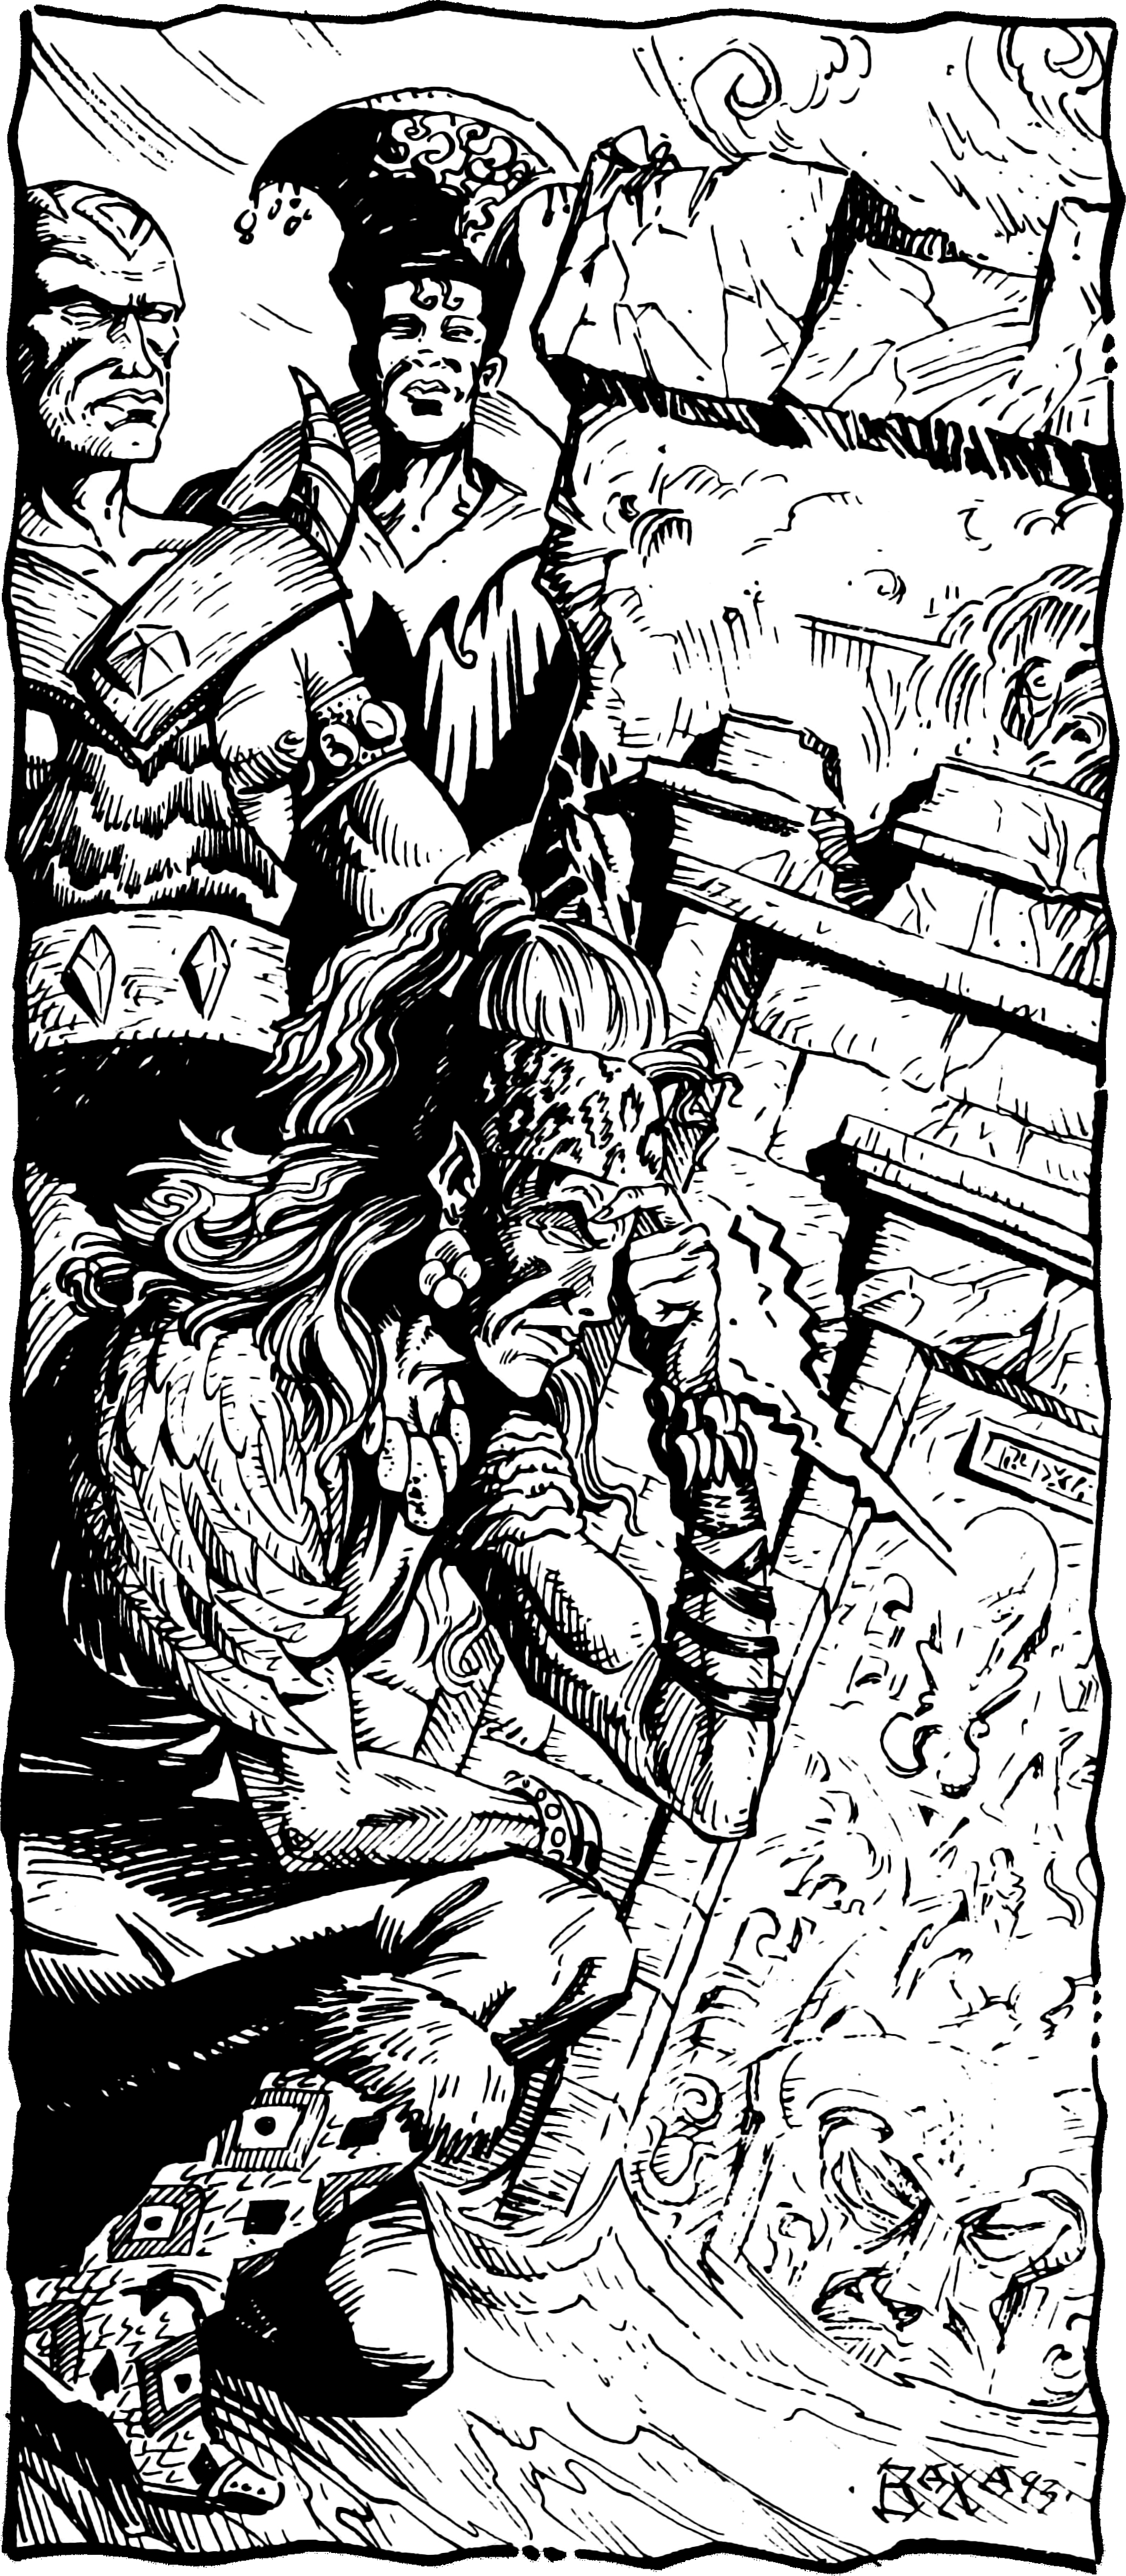
\includegraphics[width=\columnwidth-6mm]{images/cleric-4.png}
\par\textit{\small\textcopyright Wizards of the Coast, 2020.}
\end{figure}

\begin{figure*}[b]
\centering
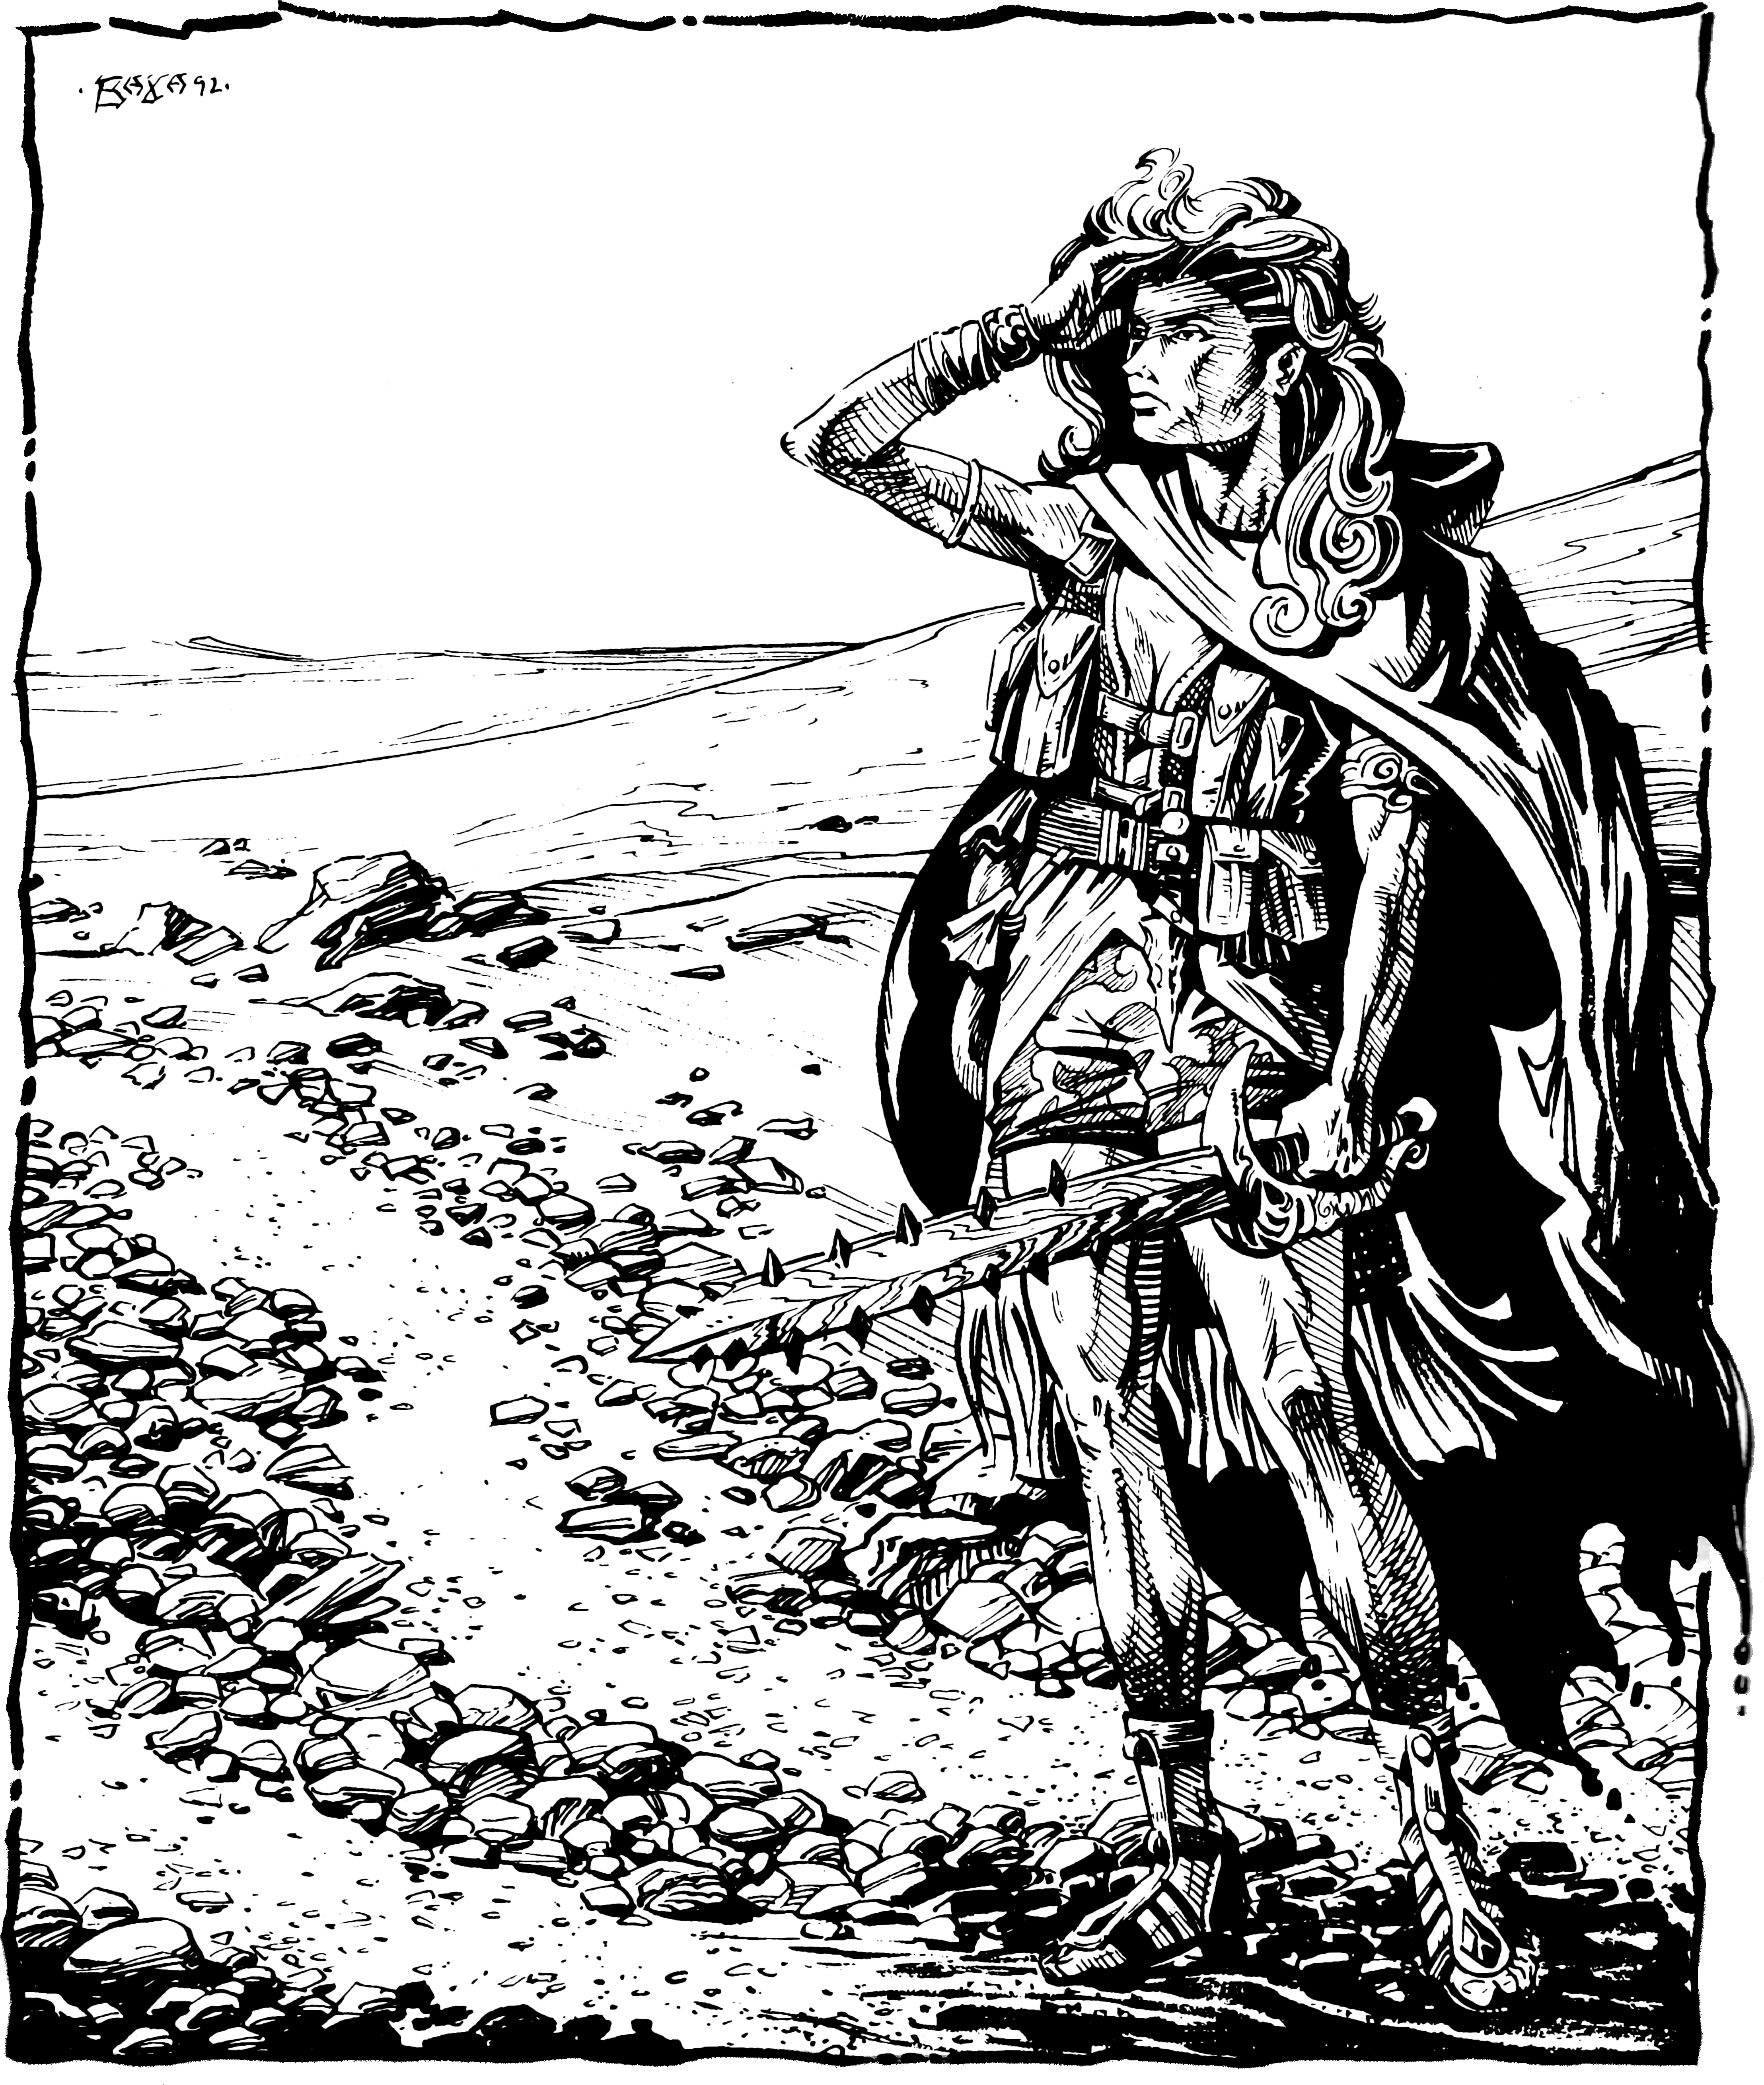
\includegraphics[width=\textwidth]{images/adventurer-1.png}
\par\textit{\small\textcopyright Wizards of the Coast, 2020.}
\end{figure*}

\clearpage
\Class{Barbarian}
{Gith's blood! I will hunt that wizard down and skin him alive.}{Borac, mul barbarian}

Brutality is a way of life in Athas, as much in some of the cities as in the dwindling tribes of Athas' harsh wastes. Cannibal headhunting halflings (who occasionally visit Urik from the Forest Ridge) sometimes express shock at the savagery and bloodshed of the folk that call themselves ``civilized'' and live between walls of stone. They would be more horrified if they were to see the skull piles of Draj, experience the Red Moon Hunt in Gulg, or watch a seemingly docile house slave in Eldaarich rage as she finally ``goes feral'', taking every frustration of her short cruel life out on whoever happens to be closest to hand. Nibenese sages claim that the potential for savagery is in every sentient race, and the history of Athas seems to support their claim.

Some on Athas have turned their brutality into an art of war. They are known as ``brutes'', ``barbarians'' or ``feral warriors'' and they wear the name with pride. Impious but superstitious, cunning and merciless, fearless and persistent, they have carved a name for their martial traditions out of fear and blood.

\WarriorTable{The Barbarian}{
1st  & +1             & +2  & +0 & +0 & Fast movement, rage 1/day               \\
2nd  & +2             & +3  & +0 & +0 & Uncanny dodge                           \\
3rd  & +3             & +3  & +1 & +1 & Wasteland trap sense +1                 \\
4th  & +4             & +4  & +1 & +1 & Rage 2/day                              \\
5th  & +5             & +4  & +1 & +1 & Improved uncanny dodge                  \\
6th  & +6/+1          & +5  & +2 & +2 & Wasteland trap sense +2                 \\
7th  & +7/+2          & +5  & +2 & +2 & Damage reduction 1/--                   \\
8th  & +8/+3          & +6  & +2 & +2 & Bonus feat, rage 3/day                  \\
9th  & +9/+4          & +6  & +3 & +3 & Greater rage, wasteland trap sense +3   \\
10th & +10/+5         & +7  & +3 & +3 & Damage reduction 2/--                   \\
11th & +11/+6/+1      & +7  & +3 & +3 & Bonus feat                              \\
12th & +12/+7/+2      & +8  & +4 & +4 & Rage 4/day, wasteland trap sense +4     \\
13th & +13/+8/+3      & +8  & +4 & +4 & Indomitable will, damage reduction 3/-- \\
14th & +14/+9/+4      & +9  & +4 & +4 & Bonus feat                              \\
15th & +15/+10/+5     & +9  & +5 & +5 & Tireless rage, wasteland trap sense +5  \\
16th & +16/+11/+6/+1  & +10 & +5 & +5 & Damage reduction 4/--, rage 5/day       \\
17th & +17/+12/+7/+2  & +10 & +5 & +5 & Bonus feat, mighty rage                 \\
18th & +18/+13/+8/+3  & +11 & +6 & +6 & Wasteland trap sense +6                 \\
19th & +19/+14/+9/+4  & +11 & +6 & +6 & Damage reduction 5/--                   \\
20th & +20/+15/+10/+5 & +12 & +6 & +6 & Bonus feat, rage 6/day                  \\
}

\begin{figure}[t!]
\centering
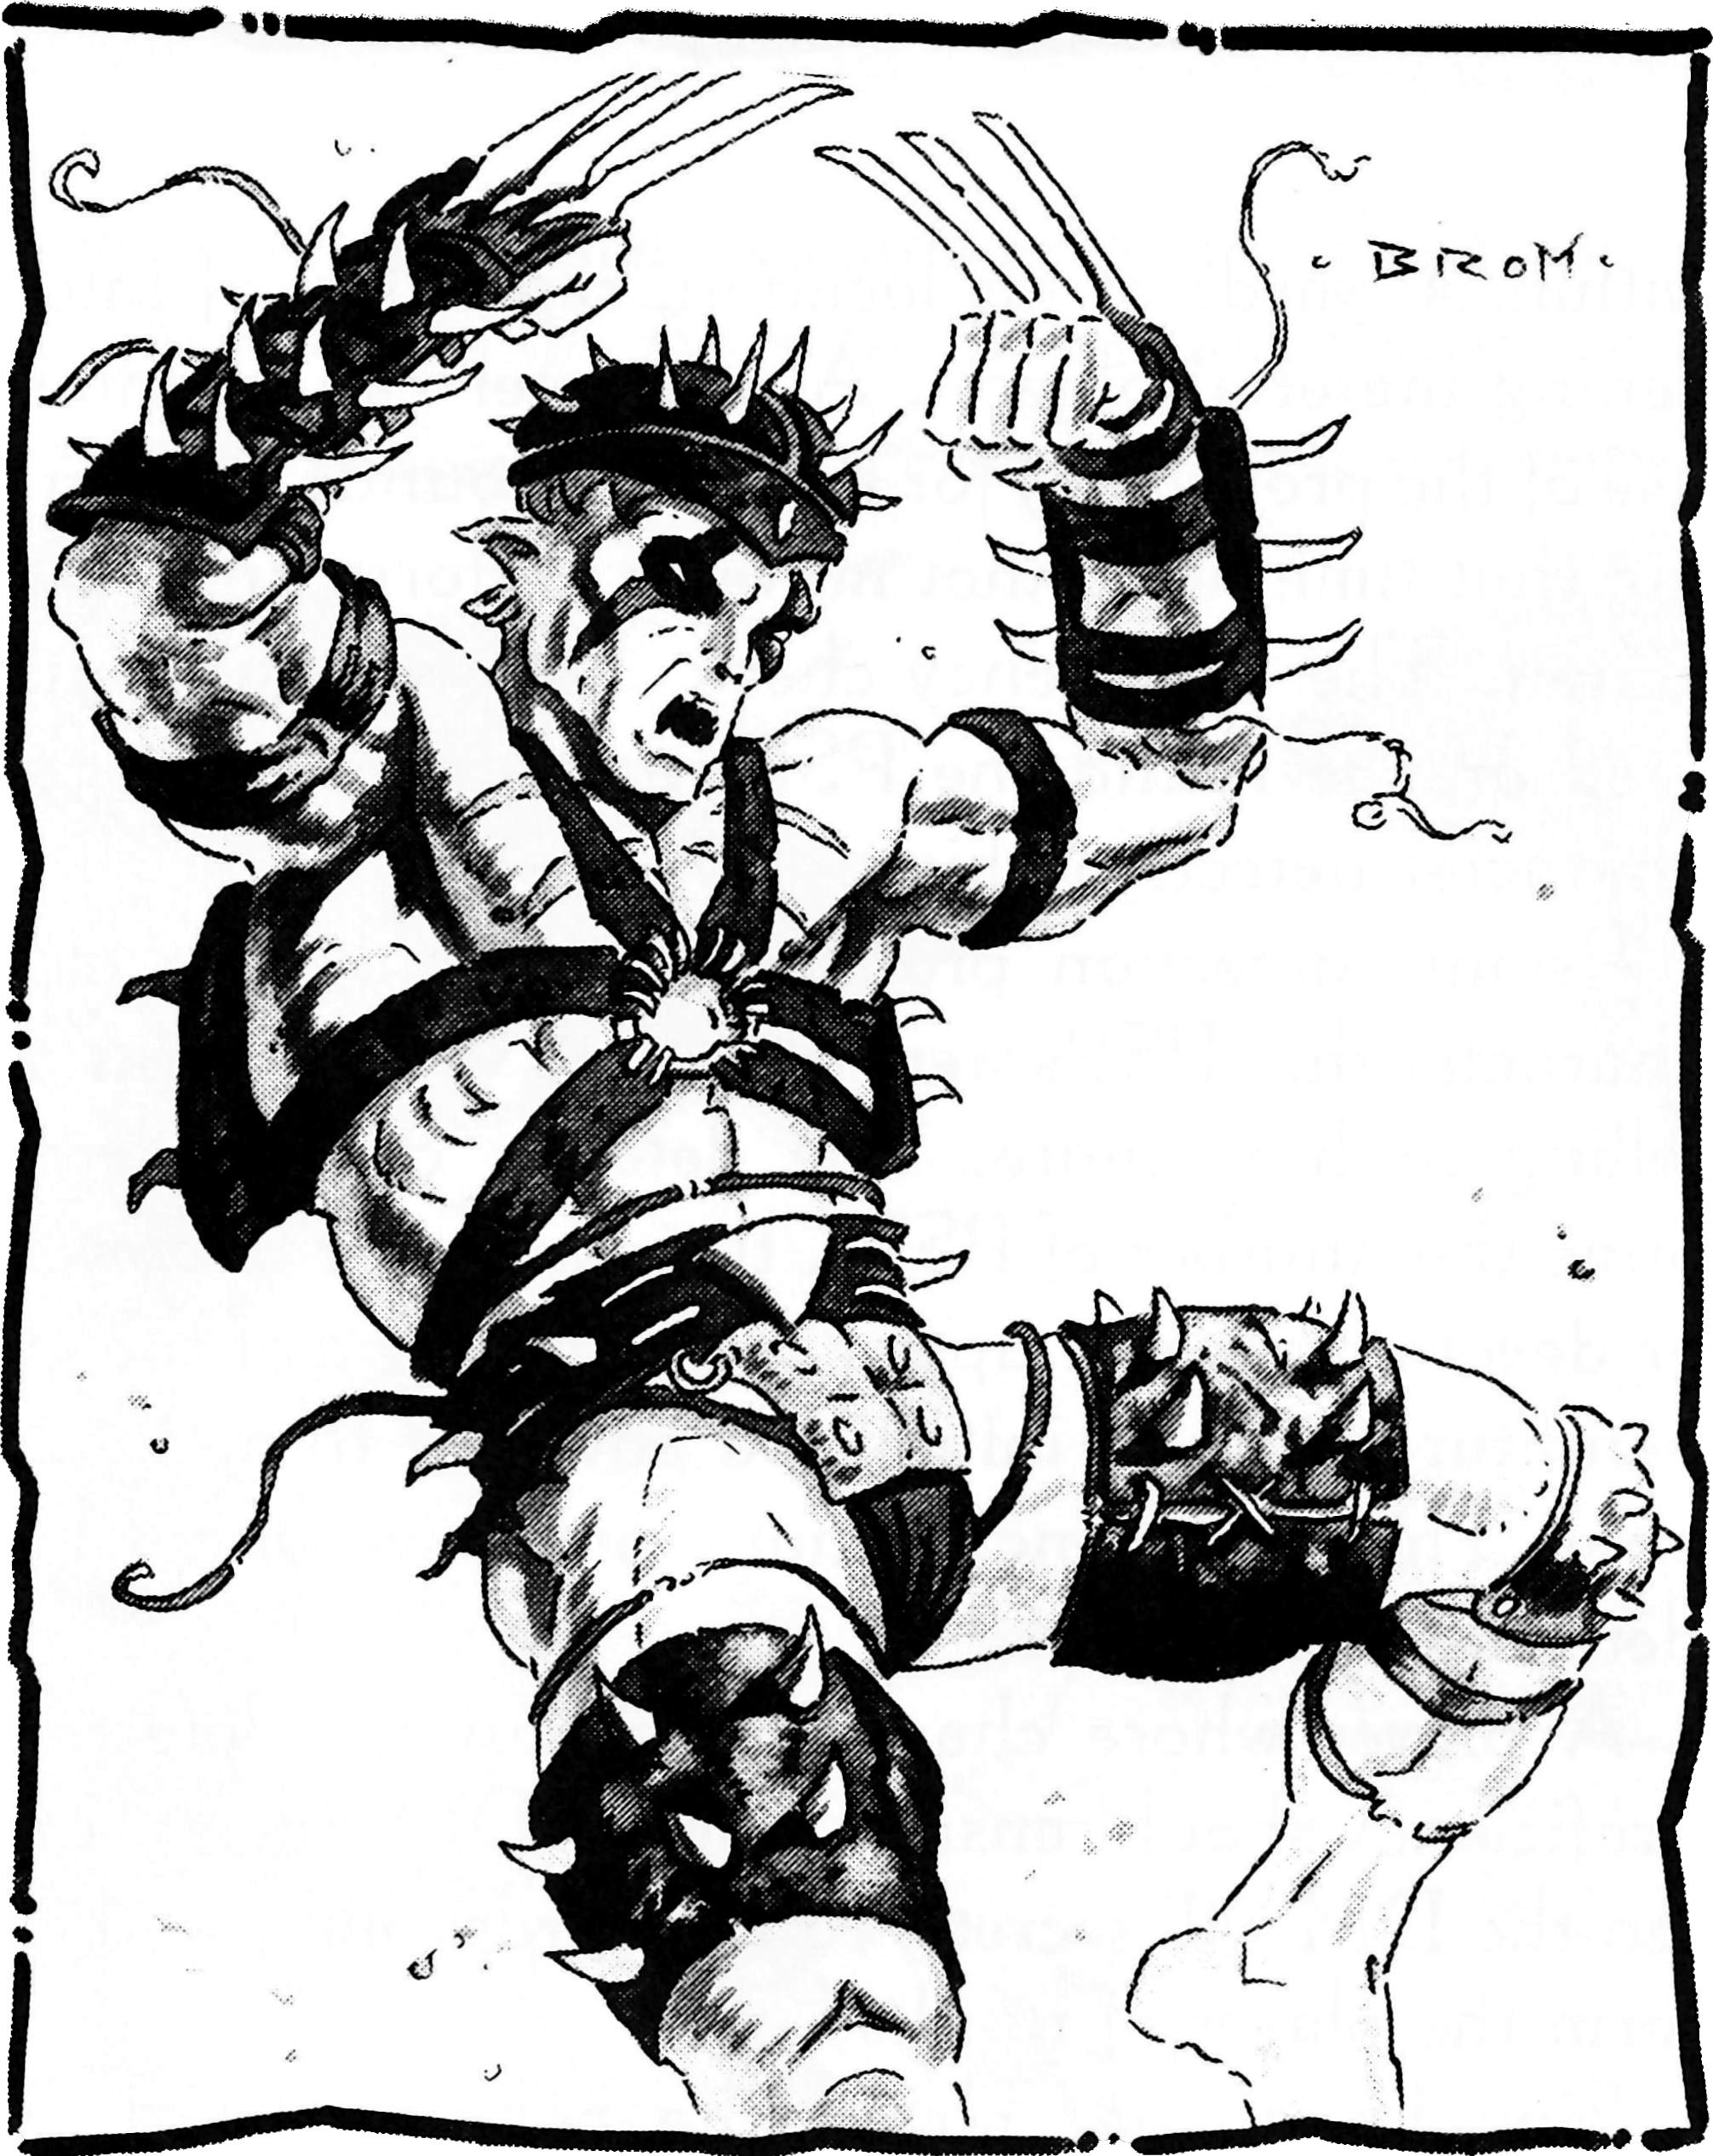
\includegraphics[width=\columnwidth]{images/barbarian-1.png}
\WOTC
\end{figure}

\subsection{Making a Barbarian}

The barbarian is a fearsome warrior, compensating for lack of training and discipline with bouts of powerful rage. While in this berserk fury, barbarians become stronger and tougher, better able to defeat their foes and withstand attacks. These rages leave barbarians winded; at first they only have the energy for a few such spectacular displays per day, but those few rages are usually sufficient.

\textbf{Races:} Humans are often barbarians, many having been raised in the wastes or escaped from slavery. Half-elves sometimes become barbarians, having been abandoned by their elven parents to the desert to survive on their own; if more of them survived they would be quite numerous. Dwarves are very rarely barbarians, but their mul half-children take to brutishness like a bird takes to flight, living by their wits and strengths in the wastes. Muls have a particular inclination this way of life, and very often ``go feral'' in the wilderness after escaping slavery in the city. Elves rarely take to the barbarian class; those that do are usually from raiding tribes such as the Silt Stalkers. Half-giants readily take the barbarian class. Despite their feral reputations, halflings rarely become barbarians; their small statures and weak strength adapts them better for the ranger class. Likewise, despite their wild nature, thri-kreen are rarely barbarians since their innate memories allow them to gain more specialized classes, such as ranger, without training. Pterrans of the Forest Ridge occasionally become barbarians, but like halflings they more often favor the ranger class.

\textbf{Alignment:} Barbarians are never lawful---their characteristic rage is anything but disciplined and controlled. Many barbarians in the cities are often rejects from the regular army, unable to bear regular discipline or training. Some may be honorable, but at heart they are wild. At best, chaotic barbarians are free and expressive. At worst, they are thoughtlessly destructive.

\subsection{Game Rule Information}
\textbf{Alignment:} Any nonlawful.

\textbf{Hit Die:} d12.

\subsubsection{Class Skills}
\skill{Autohypnosis} (Wis), \skill{Climb} (Str), \skill{Craft} (Int), \skill{Escape Artist} (Des), \skill{Handle Animal} (Cha), \skill{Intimidate} (Cha), \skill{Jump} (Str), \skill{Knowledge} (nature) (Int), \skill{Listen} (Wis), \skill{Profession} (Wis), \skill{Ride} (Dex), and \skill{Survival} (Wis).

\textbf{Skill Points per Level:} 4 + Int modifier ($\times4$ at 1st level).

\subsubsection{Class Features}

\textbf{Weapon and Armor Proficiency:} A barbarian is proficient with all simple and martial weapons, light armor, medium armor, and shields (except tower shields).

\textbf{Fast Movement (Ex):} A barbarian's land speed is faster than the norm for his race by +3 meters. This benefit applies only when he is wearing no armor, light armor, or medium armor and not carrying a heavy load. Apply this bonus before modifying the barbarian's speed because of any load carried or armor worn.

\textbf{Rage (Ex):} A barbarian can fly into a rage a certain number of times per day. In a rage, a barbarian temporarily gains a +4 bonus to Strength, a +4 bonus to Constitution, and a +2 morale bonus on Will saves, but he takes a $-2$ penalty to Armor Class. The increase in Constitution increases the barbarian's hit points by 2 points per level, but these hit points go away at the end of the rage when his Constitution  score drops back to normal. (These extra hit points are not lost first the way temporary hit points are.) While raging, a barbarian cannot use any Charisma-, Dexterity-, or Intelligence-based skills (except for \skill{Balance}, \skill{Escape Artist}, \skill{Intimidate}, and \skill{Ride}), the \skill{Concentration} skill, or any abilities that require patience or concentration, nor can he cast spells or activate magic items that require a command word, a spell trigger (such as a wand), or spell completion (such as a scroll) to function. He can use any feat he has except \feat{Combat Expertise}, item creation feats, and metamagic feats. A fit of rage lasts for a number of rounds equal to 3 + the character's (newly improved) Constitution modifier. A barbarian may prematurely end his rage. At the end of the rage, the barbarian loses the rage modifiers and restrictions and becomes fatigued ($-2$ penalty to Strength, $-2$ penalty to Dexterity, can't charge or run) for the duration of the current encounter (unless he is a 15th-level barbarian, at which point this limitation no longer applies).

A barbarian can fly into a rage only once per encounter. At 1st level he can use his rage ability once per day. At 4th level and every four levels thereafter, he can use it one additional time per day (to a maximum of six times per day at 20th level). Entering a rage takes no time itself, but a barbarian can do it only during his action, not in response to someone else's action. 

\textbf{Uncanny Dodge (Ex):} At 2nd level, a barbarian retains his Dexterity bonus to AC (if any) even if he is caught flat-footed or struck by an invisible attacker. However, he still loses his Dexterity bonus to AC if immobilized. If a barbarian already has uncanny dodge from a different class, he automatically gains improved uncanny dodge instead.

\textbf{Wasteland Trap Sense (Ex):} Starting at 3rd level, a barbarian gains a +1 bonus on Reflex saves made to avoid traps and natural hazards, and a +1 dodge bonus to AC against attacks made by traps and natural hazards. These bonuses rise by +1 every three barbarian levels thereafter (6th, 9th, 12th, 15th, and 18th level). Trap sense bonuses gained from multiple classes stack.

\textbf{Improved Uncanny Dodge (Ex):} At 5th level and higher, a barbarian can no longer be flanked. This defense denies a rogue the ability to sneak attack the barbarian by flanking him, unless the attacker has at least four more rogue levels than the target has barbarian levels. If a character already has uncanny dodge from a second class, the character automatically gains improved uncanny dodge instead, and the levels from the classes that grant uncanny dodge stack to determine the minimum level a rogue must be to flank the character.

\begin{figure}[t!]
\centering
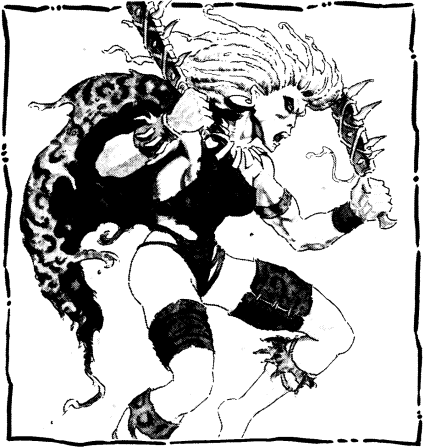
\includegraphics[width=\columnwidth]{images/halfling-1.png}
\WOTC
\end{figure}

\textbf{Damage Reduction (Ex):} At 7th level, a barbarian gains Damage Reduction. Subtract 1 from the damage the barbarian takes each time he is dealt damage from a weapon or a natural attack. At 10th level, and every three barbarian levels thereafter (13th, 16th, and 19th level), this damage reduction rises by 1 point. Damage reduction can reduce damage to 0 but not below 0.

\textbf{Bonus Feat:} At 8th level and every three levels thereafter (11th, 14th, 17th, and 20th level), a barbarian gains a bonus feat, which must be selected from the following list:
\feat{Awesome Blow},
\feat{Blind-Fight},
\feat{Cleave},
\feat{Closed Mind},
% \feat{Combat Reflexes},
Dash\textsuperscript{CW},
Destructive Rage\textsuperscript{CW},
\feat{Diehard},
\feat{Endurance},
Extend Rage\textsuperscript{CW},
Extra Rage\textsuperscript{CW},
% Faster Healing\textsuperscript{CW},
Fleet of Foot\textsuperscript{CW},
\feat{Great Cleave},
% \feat{Greater Critical},
Greater Resiliency\textsuperscript{CW},
\feat{Hard as Rock},
\feat{Hostile Mind},
\feat{Improved Bull Rush},
% \feat{Improved Critical},
% \feat{Improved Initiative},
\feat{Improved Sunder},
\feat{Innate Hunter},
Instantaneous Rage\textsuperscript{CW},
Intimidating Rage\textsuperscript{CW},
\feat{Mind Over Body},
\feat{Power Attack},
% \feat{Psionic Hole},
% \feat{Quick Draw},
\feat{Rapid Metabolism},
\feat{Reckless Offense},
\feat{Run},
Steadfast Determination\textsuperscript{PH2},
\feat{Toughness},
\feat{Track},
\feat{Wastelander}.
He must meet all the prerequisites for the feat.

\textbf{Greater Rage (Ex):} At 8th level, a barbarian's bonuses to Strength and Constitution during his rage each increase to +6, and his morale bonus on Will saves increases to +3. The penalty to AC remains at $-2$.

\textbf{Indomitable Will (Ex):} While in a rage, a barbarian of 13th level or higher gains a +4 bonus on Will saves to resist enchantment spells and telepathy powers. This bonus stacks with all other modifiers, including the morale bonus on Will saves he also receives during his rage.

\textbf{Tireless Rage (Ex):} At 15th level and higher, a barbarian no longer becomes fatigued at the end of his rage.

\textbf{Mighty Rage (Ex):} At 17th level, a barbarian's bonuses to Strength and Constitution during his rage each increase to +8, and his morale bonus on Will saves increases to +4. The penalty to AC remains at $-2$.

\subsubsection{Ex-Barbarians}
A barbarian who becomes lawful loses the ability to rage and cannot gain more levels as a barbarian. He retains all the other benefits of the class (damage reduction, fast movement, wasteland trap sense, and uncanny dodge).


\subsection{Playing a Barbarian}
All cower and stand in awe at the fury you can tap, enhancing your strength and toughness. But what do these people know of the burnt wastes of Athas, the hellish jungles of the Forest Ridge? The cruel vicissitudes of growing up in the wastes of Athas were nothing but normal to you. When your family was lost in a tembo attack, or when your entire village was either murdered or forced into slavery, how could you not know they might not had to die? These and many other brutal experiences marked you, and you now stand apart from those born into the ``comforts'' of the city-states.

\subsubsection{Religion}
Although most are profoundly superstitious, barbarians distrust the established elemental temples of the cities. Some worship the elements of fire or air or devote themselves to a famous figure. Most barbarians truly believe the sorcerer-kings to be gods, because of their undeniable power, and a few actually worship a sorcerer-king, usually the one that conquered their tribe. Such barbarians often escape menial slavery by joining an elite unit of barbarians in the service of an aggressive city-state such as Urik, Draj or Gulg.

\subsubsection{Other Classes}
Barbarians are most comfortable in the company of gladiators, and of clerics of Air and Fire. Enthusiastic lovers of music and dance, barbarians admire bardic talent, and some barbarians also express fascination with bardic poisons, antidotes and alchemical concoctions. With some justification, barbarians do not trust wizardry. Even though many barbarians manifest a wild talent, they tend to be wary of psions and Tarandan psionicists. Psychic warriors, on the other hand, are creatures after the barbarian's own heart, loving battle for its own sake. Barbarians have no special attitudes toward fighters or rogues. Barbarians admire gladiators and will ask about their tattoos and exploits, but will quickly grow bored if the gladiator does not respond boastfully.

\subsubsection{Combat}
You know that half the battle occurs before the fight even begins. You prefer to choose your battleground when you can, stalking your opponent into terrain that best suits your abilities. Once battle is joined, you become a wild frenzy of motion, striking quickly and powerfully until all your opponents are crushed. While you lack the training of the fighter, or the cunning of the gladiator, you more than compensate them through sheer power and resilience.

\subsubsection{Advancement}
Becoming a barbarian let you further tap into your feral nature, letting you become one with the savage beast in your hear, and through your training, you have learned what you must do to unlock it.

To fully utilize your barbarian abilities, you will want to focus on feats that take advantage of your superior strength and speed, such as Power Attack and Whirlwind Attack.


\subsection{Starting Packages}
\subsubsection{The Survivor}
Human Barbarian

\textbf{Ability Scores:} Str 15, Dex 13, Con 14, Int 10, Wis 12, Cha 8.

\textbf{Skills:} \skill{Climb}, \skill{Escape Artist}, \skill{Listen}, \skill{Survival}.

\textbf{Languages:} Common.

\textbf{Feat:} \feat{Great Fortitude}, \feat{Wastelander}.

\textbf{Weapons:} Carrikal (1d8/$\times$3)

Atlatl with 10 javelins (1d6/$\times$3, 12 m).

\textbf{Armor:} Scale mail (+4 AC).

\textbf{Gear:} Standard adventurer's kit, 13 cp.

\subsubsection{The Crusher}
Half-giant Barbarian

\textbf{Ability Scores:} Str 23, Dex 10, Con 18, Int 6, Wis 9, Cha 4.

\textbf{Skills:} \skill{Climb}, \skill{Intimidate}, \skill{Jump}.

\textbf{Languages:} Common.

\textbf{Feat:} \feat{Exotic Weapon Proficiency} (swatter).

\textbf{Weapons:} Swatter (3d8/$\times$4).

\textbf{Armor:} Leather (+2 AC).

\textbf{Gear:} Standard adventurer's kit, 0 cp.

\subsubsection{The Hunter}
Thri-kreen Barbarian

\textbf{Ability Scores:} Str 15, Dex 14, Con 12, Int 10, Wis 13, Cha 8.

\textbf{Skills:} \skill{Jump}, \skill{Knowledge} (nature), \skill{Search}, \skill{Survival}.

\textbf{Languages:} Kreen.

\textbf{Feat:} \feat{Track}.

\textbf{Weapons:} Four chatkchas (1d6, 6 m).

\textbf{Armor:} Heavy wooden shield (+2 AC).

\textbf{Gear:} Standard adventurer's kit, 13 cp.


\subsection{Barbarians on Athas}
\Quote{Don't make my friend angry. You won't like him when he's angry.}{Cabal, half-elven bard}

In a savage world like Athas, is only natural that some of its inhabitants have turned into barbarians. They are fierce combatants without the army training fighters receive or wild rangers without the hunting skills.

\subsubsection{Daily Life}
A barbarian is a passionate adventurer. As a survivalist, he often sees his involvement in a particular enterprise as a validation of his superior strength and resilience. In his mind, his presence alone is enough to ensure the success of a quest, adventure, or ruin raid. Even simple tasks are additional opportunities to prove his own worth by accomplishing the task with might and alacrity. Barbarians are typically hardheaded and unforgiving because of the rigors of his previous life.

\subsubsection{Notables}
It is rare for a barbarian to live long enough, or close enough to civilization, in order to become famous, but a few examples exist. Korno, a Raamite gladiator, became the leader of a group of slaves, and Korno's furious rage known from the arenas has only increased after losing everything in the Raam invasion by Dregoth. The leader of Pillage, Chilod, is a tarek know for his outbursts of rage and cruelty, being one of the most feared chiefs of the Bandit States.

\subsubsection{Organizations}
Because of their independent and sometimes downright chaotic natures, many barbarians refuse to join organizations of any kind, though they usually maintain relationships with trading houses and raiding tribes. There is no specific organization that binds barbarians together.

\subsubsection{NPC Reactions}
Many lay people cannot tell a barbarian from a ranger or a fighter until his rage overcomes him and he starts screaming and bashing. Most authority figures and templars do not appreciate barbarians since they are prone to losing control and cannot be truly trusted. Thus, they generally treat barbarians with a great deal of caution.

\subsubsection{Barbarian Lore}
Characters with ranks in \skill{Knowledge} (nature) can research barbarians to learn more about them. When a character makes a skill check, read or paraphrase the following, including the information from lower DCs.

\textbf{DC 10:} Barbarians are hot-blooded combatants who fight with great brutality and savagery.

\textbf{DC 15:} Barbarians become stronger and more resilient when they lose control.

\textbf{DC 20:} Barbarians can stand up to punishment that no other individual can endure, and their reflexes are as quick as a rogue's.
\Class{Bard}
{Some people think a club can solve any problem. Unless you're a half-giant, there are more sophisticated ways of settling a disagreement.}{Cabal, half-elven bard}

From the shadowy corners of Athas' most disreputable places hails the bard. Like their counterparts in other fantasy worlds, Athasian bards are the unquestioned masters of oral tradition and forgotten lore, but rather than sharing their lore with whoever will listen, Athasian bards guard their secrets as jealously as the sorcerer-kings harbor their water and iron. Athasian bards may sell information to the highest bidder; they peddle their services and the fruits of their knowledge, but trade secrets are what give bards an edge on the uninitiated. Bards would rather die than reveal these secrets.

Meeting a bard can be an uneasy encounter, since one never knows how the bard has chosen to devote his multiple talents. Some bards master the art of making poisons, and survive by selling these poisons and their antidotes for those who have coin to pay. Some bards master the art of entertainment, using their performances to amuse nobles and templars and gain wealth. Some become assassins, mixing their knowledge of poison and stealth to become hired hands. Bards' unique position in the Athasian society means they often overhear conversations between high-ranking templars or nobles, or they may have treated an injured person that prefers to remain anonymous. Respectable folk despise them; the powerful fear them; but in the Athasian cities, everyone eventually comes to need their services.

\WarriorTable[b{0.8cm} b{2.6cm} Z{1.4cm} Z{1.4cm} Z{1.4cm} X]{The Bard}{
1st  & +0         & +2  & +2  & +2  & Bardic music, bardic knowledge, smuggler, countersong, \emph{fascinate}, inspire courage +1\\
2nd  & +1         & +3  & +3  & +3  & Poison use, streetsmart                                  \\
3rd  & +2         & +3  & +3  & +3  & Inspire competence, \feat{Quick Draw}                    \\
4th  & +3         & +4  & +4  & +4  & Trade secret                                             \\
5th  & +3         & +4  & +4  & +4  & Mental resistance                                        \\
6th  & +4         & +5  & +5  & +5  & Improved poison use, \emph{suggestion}, quick thinking +2\\
7th  & +5         & +5  & +5  & +5  & Chance 1/day, inspire courage +2                         \\
8th  & +6/+1      & +6  & +6  & +6  & Trade secret                                             \\
9th  & +6/+1      & +6  & +6  & +6  & Inspire greatness, speed reactions                       \\
10th & +7/+2      & +7  & +7  & +7  & Special ability                                          \\
11th & +8/+3      & +7  & +7  & +7  & Quick thinking +4                                        \\
12th & +9/+4      & +8  & +8  & +8  & \emph{Song of freedom}, trade secret                     \\
13th & +9/+4      & +8  & +8  & +8  & Inspire courage +3                                       \\
14th & +10/+5     & +9  & +9  & +9  & Chance 2/day                                             \\
15th & +11/+6/+1  & +9  & +9  & +9  & Inspire heroics, special ability                         \\
16th & +12/+7/+2  & +10 & +10 & +10 & Quick thinking +6, trade secret                          \\
17th & +12/+7/+2  & +10 & +10 & +10 & Awareness                                                \\
18th & +13/+8/+3  & +11 & +11 & +11 & \emph{Mass suggestion}, \emph{mind blank}                \\
19th & +14/+9/+4  & +11 & +11 & +11 & Inspire courage +4                                       \\
20th & +15/+10/+5 & +12 & +12 & +12 & Special ability, trade secret                            \\
}

\Figure*{t}{images/bard-2.png}

\subsection{Making a Bard}
Bards receive numerous abilities they can use to survive. Many become masters of poisons, selling their illegal substances to anyone. Alone of the classes, bards hold the secrets of alchemy, creating fiery concoctions and mysterious mixes. Bards are master smugglers, selling spell components and other illegal items in the Bard's Quarters of the city-states. All bards, however, have some degree of entertainment skill. The songs of most bards can dazzle a crowd, or incite them to riot. Bards tend to learn to play a variety of instruments, or recite poetry or old legends by campfire. They can be acrobats, performing dazzling displays of physical prowess. They are often called upon as sources of information.

\textbf{Abilities:} Charisma is the most important ability for a bard, because many of their abilities and skills are affected by it. A high Dexterity improves the bard's defensive ability. Intelligence is also important because it bolster the numbers of skills he has access.

\textbf{Races:} All humanoid races of Athas can become bards. The social stigma in certain regions may be higher than others, however. For example, the loremasters of the halflings of the Jagged Cliffs are highly regarded because of the ancient secrets and histories they preserve. But in the city-states, where the Bard's Quarters are notorious, being a bard is not usually a good thing. Elven tribes often have a bard, who keeps the history of the tribe alive, its conquests and defeats. Humans are often bards, becoming performers of great talent, or assassins of deadly skill and precision. Half-elves, because of their lonely existence, often take to being bards. The prejudice they face at every stage in life can move some to become great poets or singers. Muls and half-giants make poor bards; their talents are usually better served elsewhere than the stage or the shadows of alleys. As well, thri-kreen are rarely seen as bards, relying instead upon their racial memory.

\textbf{Alignment:} Most bards are chaotic, and operate alone, brokering information, arranging deals, smuggling illegal wares such as poisons, drugs, spell components and other things. Neutral bards are the ones most likely to operate in fellowships with adventurers, or entertain in troupes with other bards. The rare lawful bards can easily secure positions as councilors or agents for templars, and noble and merchant houses. Good bards are often entertainers or lorekeepers, putting their talents to benevolent use, sometimes diagnosing poisonings and selling the proper antidotes. Evil bards are often masters of poisons and alchemy, selling their wares to anyone with the ceramic to pay.

\subsection{Game Rule Information}

\textbf{Hit Die:} d6.

\subsubsection{Class Skills}
\skill{Appraise} (Int), \skill{Balance} (Dex), \skill{Bluff} (Cha), \skill{Climb} (Str), \skill{Craft} (Int), \skill{Decipher Script} (Int), \skill{Diplomacy} (Cha), \skill{Disguise} (Cha), \skill{Escape Artist} (Dex), \skill{Forgery} (Int), \skill{Gather Information} (Cha), \skill{Heal} (Wis), \skill{Hide} (Dex), \skill{Intimidate} (Cha), \skill{Jump} (Str), \skill{Knowledge} (all skills individually) (Int), \skill{Listen} (Wis), \skill{Move Silently} (Dex), \skill{Perform} (Cha), \skill{Profession} (Wis), \skill{Ride} (Dex), \skill{Search} (Int), \skill{Sense Motive} (Wis), \skill{Sleight of Hand} (Dex), \skill{Speak Language} (N/A), \skill{Tumble} (Dex), \skill{Use Magic Device} (Cha), \skill{Use Psionic Device} (Cha), and \skill{Use Rope} (Dex).

\textbf{Skill Points per Level:} 6 + Int modifier ($\times4$ at 1st level).

\subsubsection{Class Features}

\textbf{Weapon and Armor Proficiency:} You are proficient in all simple weapons, plus the bard's friend, all crossbows, garrote, greater blowgun, whip and widow's knife. You are proficient in light armor, but not shields.

\textbf{Bardic Knowledge:} A bard may make a special bardic knowledge check with a bonus equal to his bard level + his Intelligence modifier to see whether he knows some relevant information about local notable people, legendary items, or noteworthy places. (If the bard has 5 or more ranks in \skill{Knowledge} (history), he gains a +2 bonus on this check.)

A successful bardic knowledge check will not reveal the powers of a magic item but may give a hint as to its general function. A bard may not take 10 or take 20 on this check; this sort of knowledge is essentially random.

\Table{}{p{0.6cm} X}{
\tableheader DC & \tableheader Type of Knowledge\\
10 & Common, known by at least a substantial minority of the local population.\\
20 & Uncommon but available, known by only a few people legends.\\
25 & Obscure, known by few, hard to come by.\\
30 & Extremely obscure, known by very few, possibly forgotten by most who once knew it, possibly known only by those who don't understand the significance of the knowledge.}

\textbf{Bardic Music:} Once per day per bard level, a bard can use his song or poetics to produce magical effects on those around him (usually including himself, if desired). While these abilities fall under the category of bardic music and the descriptions discuss singing or playing instruments, they can all be activated by reciting poetry, chanting, singing lyrical songs, singing melodies, whistling, playing an instrument, or playing an instrument in combination with some spoken performance. Each ability requires both a minimum bard level and a minimum number of ranks in the \skill{Perform} skill to qualify; if a bard does not have the required number of ranks in at least one \skill{Perform} skill, he does not gain the bardic music ability until he acquires the needed ranks. A bard cannot use \skill{Perform} (arena fighting) to use his bardic music abilities.

Starting a bardic music effect is a standard action. Some bardic music abilities require concentration, which means the bard must take a standard action each round to maintain the ability. Even while using bardic music that doesn't require concentration, a bard cannot cast spells, activate magic items by spell completion (such as scrolls), spell trigger (such as wands), or command word. Just as for casting a spell with a verbal component, a deaf bard has a 20\% chance to fail when attempting to use bardic music. If he fails, the attempt still counts against his daily limit.

\textit{Countersong (Su):} A bard with 3 or more ranks in a \skill{Perform} skill can use his music or poetics to counter magical effects that depend on sound (but not spells that simply have verbal components). Each round of the countersong, he makes a \skill{Perform} check. Any creature within 9 meters of the bard (including the bard himself) that is affected by a sonic or language-dependent magical attack may use the bard's \skill{Perform} check result in place of its saving throw if, after the saving throw is rolled, the \skill{Perform} check result proves to be higher. If a creature within range of the countersong is already under the effect of a noninstantaneous sonic or language-dependent magical attack, it gains another saving throw against the effect each round it hears the countersong, but it must use the bard's \skill{Perform} check result for the save. Countersong has no effect against effects that don't allow saves. The bard may keep up the countersong for 10 rounds.

\textit{Fascinate (Sp):} A bard with 3 or more ranks in a \skill{Perform} skill can use his music or poetics to cause one or more creatures to become fascinated with him. Each creature to be fascinated must be within 27 meters, able to see and hear the bard, and able to pay attention to him. The bard must also be able to see the creature. The distraction of a nearby combat or other dangers prevents the ability from working. For every three levels a bard attains beyond 1st, he can target one additional creature with a single use of this ability.

To use the ability, a bard makes a \skill{Perform} check. His check result is the DC for each affected creature's Will save against the effect. If a creature's saving throw succeeds, the bard cannot attempt to fascinate that creature again for 24 hours. If its saving throw fails, the creature sits quietly and listens to the song, taking no other actions, for as long as the bard continues to play and concentrate (up to a maximum of 1 round per bard level). While fascinated, a target takes a $-4$ penalty on skill checks made as reactions, such as \skill{Listen} and \skill{Spot} checks. Any potential threat requires the bard to make another \skill{Perform} check and allows the creature a new saving throw against a DC equal to the new \skill{Perform} check result.

Any obvious threat, such as someone drawing a weapon, casting a spell, or aiming a ranged weapon at the target, automatically breaks the effect. Fascinate is an enchantment (compulsion), mind-affecting ability.

\textit{Inspire Courage (Su):} A bard with 3 or more ranks in a \skill{Perform} skill can use song or poetics to inspire courage in his allies (including himself), bolstering them against fear and improving their combat abilities. To be affected, an ally must be able to hear the bard sing. The effect lasts for as long as the ally hears the bard sing and for 5 rounds thereafter. An affected ally receives a +1 morale bonus on saving throws against charm and fear effects and a +1 morale bonus on attack and weapon damage rolls. At 7th level, and every six bard levels thereafter, this bonus increases by 1 (+2 at 7th, +3 at 13th, and +4 at 19th). Inspire courage is a mind-affecting ability.

\textit{Inspire Competence (Su):} A bard of 3rd level or higher with 6 or more ranks in a \skill{Perform} skill can use his music or poetics to help an ally succeed at a task. The ally must be within 9 meters and able to see and hear the bard. The bard must also be able to see the ally.

The ally gets a +2 competence bonus on skill checks with a particular skill as long as he or she continues to hear the bard's music. Certain uses of this ability are infeasible. The effect lasts as long as the bard concentrates, up to a maximum of 2 minutes. A bard can't inspire competence in himself. Inspire competence is a mind-affecting ability.

\textit{Suggestion (Sp):} A bard of 6th level or higher with 9 or more ranks in a \skill{Perform} skill can make a \spell{suggestion} (as the spell) to a creature that he has already fascinated. Using this ability does not break the bard's concentration on the fascinate effect, nor does it allow a second saving throw against the fascinate effect.

Making a \emph{suggestion} doesn't count against a bard's daily limit on bardic music \skill{perform}ances. A Will saving throw (DC 10 + \onehalf bard's level + bard's Cha modifier) negates the effect. This ability affects only a single creature (but see \emph{mass suggestion}, below). \emph{Suggestion} is an enchantment (compulsion), mind-affecting, language dependent ability.

\textit{Inspire Greatness (Su):} A bard of 9th level or higher with 12 or more ranks in a \skill{Perform} skill can use music or poetics to inspire greatness in himself or a single willing ally within 9 meters, granting him or her extra fighting capability. For every three levels a bard attains beyond 9th, he can target one additional ally with a single use of this ability (two at 12th level, three at 15th, four at 18th). To inspire greatness, a bard must sing and an ally must hear him sing. The effect lasts for as long as the ally hears the bard sing and for 5 rounds thereafter. A creature inspired with greatness gains 2 bonus Hit Dice (d10s), the commensurate number of temporary hit points (apply the target's Constitution modifier, if any, to these bonus Hit Dice), a +2 competence bonus on attack rolls, and a +1 competence bonus on Fortitude saves. The bonus Hit Dice count as regular Hit Dice for determining the effect of spells that are Hit Dice dependent. Inspire greatness is a mind-affecting ability.

\textit{Song of Freedom (Sp):} A bard of 12th level or higher with 15 or more ranks in a \skill{Perform} skill can use music or poetics to create an effect equivalent to the \spell{break enchantment} spell (caster level equals the character's bard level). Using this ability requires 1 minute of uninterrupted concentration and music, and it functions on a single target within 9 meters. A bard can't use song of freedom on himself.

\Figure{t}{images/bard-1.png}

\textit{Inspire Heroics (Su):} A bard of 15th level or higher with 18 or more ranks in a \skill{Perform} skill can use music or poetics to inspire tremendous heroism in himself or a single willing ally within 9 meters. For every three bard levels the character attains beyond 15th, he can inspire heroics in one additional creature. To inspire heroics, a bard must sing and an ally must hear the bard sing for a full round. A creature so inspired gains a +4 morale bonus on saving throws and a +4 dodge bonus to AC. The effect lasts for as long as the ally hears the bard sing and for up to 5 rounds thereafter. Inspire heroics is a mind-affecting ability.

\textit{Mass Suggestion (Sp):} This ability functions like \emph{suggestion}, above, except that a bard of 18th level or higher with 21 or more ranks in a \skill{Perform} skill can make the suggestion simultaneously to any number of creatures that he has already fascinated. \emph{Mass suggestion} is an enchantment (compulsion), mind-affecting, language-dependent ability.

\textbf{Smuggler (Ex):} A bard receives a +1 insight bonus to \skill{Bluff} and \skill{Sleight of Hand} checks for every two bard levels.

\textbf{Poison Use:} Bards are trained in the use of poisons, and as of 2nd level, never risk accidentally poisoning themselves when applying poison to a blade.

\textbf{Streetsmart (Ex):} When a bard reaches 2nd level, he gets a +2 competence bonus to \skill{Gather Information} and \skill{Intimidate} checks.

\textbf{Quick Draw:} Bards learn to strike quickly and without warning. At 3rd level, a bard gains \feat{Quick Draw} as a bonus feat.

\textbf{Trade Secrets:} At 4th level and every four levels thereafter (8th, 12th, 16th, and 20th level), a bard learns a trade secret chosen from the list below.

\textit{Alchemy Dealer (Ex):} A bard with this trade secret pays \onehalf of the market price for raw materials needed to craft alchemical items.

\textit{Coolheaded:} A bard with this trade secret may take 10 on \skill{Bluff} and \skill{Diplomacy} checks. A bard must be at least 12th level to select this trade secret.

\textit{Improvised Materials (Ex):} A bard with this trade secret can craft poisons from raw materials at hand instead of relying on specific ingredients. Doing so increases the \skill{Craft} (poisonmaking) check DC by 5 but otherwise has no effect on the poison's potency.

\textit{Poison Dealer (Ex):} A bard with this trade secret pays \onehalf of the market price for raw materials needed to craft poisons.

\textit{Poisonbane (Ex):} A bard with this trade secret receives a +4 insight bonus to \skill{Craft} (alchemy) checks when creating antitoxin and poison antidotes.

\textit{Poison Resistance (Ex):} A bard with this trade secret receives a +4 bonus to saving throws against poisons.

\textit{Scorpion's Touch:} A bard with this trade secret adds +1 to the save DC of all poisons applied by him. This trade secret may be chosen more than once, and its effects stack.

\textit{Skilled:} A bard with this trade secret adds \onequarter your bard level as a competence bonus to one of the following skills: \skill{Appraise}, \skill{Bluff}, \skill{Craft}, \skill{Diplomacy}, \skill{Heal}, \skill{Perform}, \skill{Profession}, \skill{Sense Motive} or \skill{Sleight of Hand}. This trade secret may be chosen more than once, each time it applies to a different skill.

\textit{Smokestick Application (Ex):} A bard with this trade secret can combine inhaled poisons with smokesticks. All creatures within the area the smokestick covers (3-m cube) are affected by the poison you applied to the smokestick.

\textit{Versatile:} A bard with this trade secret selects any two non-class skills to be considered class skills.


\textbf{Mental Resistance (Ex):} Bards carry many dark secrets they would prefer remain secret. This, combined with a large amount of knowledge based on half-truths and false rumors makes your mind unreliable to those who would seek to mentally affect it. A 5th level bard receives a +2 morale bonus to saves made against telepathic powers and enchantment (charm) spells.

\textbf{Improved Poison Use (Ex):} At 6th level, a bard can apply poison to a weapon as a free action without provoking attacks of opportunity.

\textbf{Quick Thinking (Ex):} Bards often find themselves in a tight spot where they have to act quickly, whether it is to escape a templar patrol or strike first when in confrontation with a foe. At 6th level, a bard gets a +2 bonus on initiative checks. This bonus increases by 2 at every five levels thereafter (+4 at 11th, and +6 at 16th level).

\textbf{Chance (Ex):} Bards live on the edge in many ways. At 7th level, a bard may reroll one single d20 roll once per day, but have to keep the latter result---for better or for worse. At 14th level, a bard may use this ability two times per day.

\textbf{Speed Reactions (Ex):} Beginning at 9th level, when a bard uses the attack action or full attack action in melee, he may subtract a number from all melee attack rolls and add the same number to his initiative. This number may not exceed his base attack bonus. He may not make ranged attacks this round. The initiative increase takes effect on the next round. The new initiative is his initiative for the remainder of the combat, unless you were to use speed reactions again, which would increase your initiative further.

\textbf{Special Ability:} On attaining 10th level, and at every five levels thereafter (15th, and 20th), a bard gains a special ability of his choice from among the following options.

\textit{Defensive Roll (Ex):} A bard learns how to avoid a potentially lethal blow to take less damage from it than he otherwise would. Once per day, when he would be reduced to 0 or fewer hit points by damage in combat (from a weapon or other blow, not a spell or special ability), the bard can attempt to roll with the damage. To use this ability, the bard must attempt a Reflex saving throw (DC = damage dealt). If the save succeeds, he takes only half damage from the blow; if it fails, he takes full damage. He must be aware of the attack and able to react to it in order to execute his defensive roll---if he is denied his Dexterity bonus to AC, he can't use this ability. Since this effect would not normally allow a character to make a Reflex save for half damage, the rogue's evasion ability does not apply to the defensive roll.

\textit{Infiltrator (Ex):} When trying to mimic another person's speech, writing, and behavior, the bard roll the checks for \skill{Bluff}, \skill{Disguise} and \skill{Forgery} with advantage. This ability only works for the first time he tries to impersonate.

\textit{Silver Tongue (Ex):} His constant dealing with others gives him a keen sense of how to make them believe his lies. A bard may attempt a retry of one of the following skills, but with disadvantage: \skill{Bluff}, \skill{Diplomacy}, \skill{Disguise}, or \skill{Intimidate}. A bard may gain this special ability multiple times, selecting an additional skill for it to apply to each time.

\textit{Slippery Mind (Ex):} If a bard with slippery mind is affected by an enchantment spell or effect or a telepathy power or effect and fails his saving throw, he can attempt it again 1 round later at the same DC. He gets only this one extra chance to succeed on his saving throw.

\textbf{Awareness (Ex):} At 17th level, you are never caught flat-footed and always act in the surprise round.

\textit{Mind Blank (Sp):} At 18th level your mind becomes completely sealed against involuntary intrusion as per the \spell{mind blank} spell. This spell-like ability is always considered active.


\subsection{Playing a Bard}
You are a master of oral tradition and lore, and a true artist, but you share your talents only with those who can afford to pay you.

You are an artist. You are the center of attention (whenever you want to), the person everyone wants to talk to, the ``face'' of the party. Even if you aren't the most attractive or charismatic member of your group, your unequaled skill at performance arts creates an irresistible appeal born of justified confidence. You are more than just light entertainment, though. Your target rarely survives the encounter if you don't want him to.

You might adventure because you desire entertainment. Someone with your smarts gets bored easily. Alternatively, you may have been blacklisted on your current location because of a ``business transaction'' gone wrong. You have to keep moving, and adventuring offers you a regular change of scenery. In any case, a life of adventure allows you to see new things, meet interesting people, and get some silvers in the process.

\subsubsection{Religion}
No central bardic organization exists, and more often than not bards have no particular penchant for religion. Some may worship the elements, fearing the power of the elemental forces, and most bards tend to relate to the Air ever-changing nature, but bards that worship sorcerer-kings are rare. A lifestyle of breaking the rules of the city-states does not lend one to worship the lawgivers.

\subsubsection{Other Classes}
Bards face life as it comes, and usually hold no special grudge or awe for any one class. They usually approach other's profession on the basis of how it can help them at the moment. Clerics and druids are respected for their devotion to a divine force, but usually not held in awe. Fighters, gladiators and rangers can be useful as sword-arms but are otherwise useless to the bard. Bards do not view wizards with the same aversion as others might view them, since bards sell them their components.

\subsubsection{Combat}
A bard rarely seeks to initiate combat---instead he skulks about, looking for an opportunity to strike swiftly, using his poisons to their greatest advantage. Your work best with teammates, maneuvering to get flanks and help bring down opponents with your various poisons. Use your bardic music to bolster your allies and distract your opponents while the real heavy hitters in your group mop them up.

\subsubsection{Advancement}
You have a flexibility in building your talents unrivaled by any other class. You can either emphasize on ability or nurse a broad range of abilities. In most cases, feats that consistently improve your talents are more useful than feats that function in only certain situations.

% Many feats in the Athasian Emporium supplement make the most of your poison abilities. 
As you advance in the class, continue to max out your ranks in \skill{Bluff} and \skill{Perform}, and invest skill points in \skill{Gather Information} and \skill{Sleight of Hand}. \feat{Improved Feint} is an excellent choice with your expertise in \skill{Bluff}, and \feat{Greasing the Wheels} if perfect for getting around templar inspections. If you play up the assassin aspect of this class, consider magic (or psionic) items that help you cloak your true intentions, such as an amulet of proof against detection and location or a veil of lies.

When multiclassing or taking a level in a prestige class, find combinations that further broaden your abilities or that increase your flexibility. The prestige classes \class{Poisonmaster}, \class{Dune Trader}, and \class{Assassin} deserve special mention. They are a great combination with the bard class.


\subsection{Starting Packages}
\subsubsection{The Assassin}
Elf Bard

\textbf{Ability Scores:} Str 13, Dex 17, Con 10, Int 10, Wis 14, Cha 8.

\textbf{Skills:} \skill{Climb}, \skill{Disguise}, \skill{Hide}, \skill{Move Silently}, \skill{Open Lock}, \skill{Spot}.

\textbf{Languages:} Elven, Common.

\textbf{Feat:} \feat{Stealthy}.

\textbf{Weapons:} Bard's friend (1d4/18-20)

Shortbow with 20 arrows (1d6/$\times$3, 18 m).

\textbf{Armor:} Studded leather (+3 AC).

\textbf{Gear:} Standard adventurer's kit, thieves' tools, musical instrument, 9 cp.

\subsubsection{The Information Smuggler}
Human Bard

\textbf{Ability Scores:} Str 8, Dex, 12, Con 10, Int 15, Wis 14, Cha 13.

\textbf{Skills:} \skill{Bluff}, \skill{Decipher Script}, \skill{Diplomacy}, \skill{Gather Information}, \skill{Knowledge} (local), \skill{Listen}, \skill{Sense Motive}.

\textbf{Languages:} City language, Common, Elven.

\textbf{Feat:} \feat{Investigator}, \feat{Negotiator}.

\textbf{Weapons:} Widow's knife (1d4/$\times$3)

Light crossbow with 20 bolts (1d8/19-20, 24 m).

\textbf{Armor:} Leather armor (+2 AC).

\textbf{Gear:} Standard adventurer's kit, 4 cp.

\subsubsection{The Poisoner}
Half-elf Bard

\textbf{Ability Scores:} Str 8, Dex 15, Con 10, Int 15, Wis 14, Cha 6.

\textbf{Skills:} \skill{Appraise}, \skill{Craft} (alchemy), \skill{Craft} (poisonmaking), \skill{Knowledge} (local), \skill{Sleight of Hand}.

\textbf{Languages:} City language, Common, Elven.

\textbf{Feat:} \feat{Skill Focus} (Craft [poisonmaking]).

\textbf{Weapons:} Bard's friend (1d4/18-20)

Blowgun with 20 needles (1, 3 m).

\textbf{Armor:} Shell armor (+4 AC).

\textbf{Gear:} Standard adventurer's kit, smokestick, 4 cp.


\subsection{Bards on Athas}
\Quote{She was a rare beauty: charming, graceful, talented. It's too bad she killed my boss.}{Talos, mul bodyguard}

Athasian bards use songs and tales as their tools of trade. A bard is a person of wit and camaraderie. Despite having few other talents to offer, the bard is a welcome source of entertainment and information across Athas. However, bards are noted to be extremely untrustworthy and even ruthless---they often sell their skills as assassins and poison alchemists to the highest bidder.

In the cities, bards often become tools of the nobility. They're commonly hired by one noble house and sent to another as a gift. The bards are sent not only to entertain, but usually to perform some other subtle task as well (such as robbery, espionage, or even assassination).

Nobles consider it rude to turn down the gift of a bard or bard company. However, when presented with a troop of bards from one's worst enemy, it's sometimes better to be rude and turn them away, for the consequences of their visit could be downright deadly. To get around this, the noble who hired them sometimes disguises their approach by having another noble send them. A very complicated collage of intrigue and deceit is often woven wherever bards are involved.

\subsubsection{Daily Life}
The way a bard behaves depends on his individual sense of morality. Some think nothing of adopting false identities, smuggling forbidden goods, or even coldblooded assassination. Other bards find themselves driven to use their skills to entertain and help people.

Bards can become great leaders. With their quick wits and great charisma, bards would be natural leaders were it not for their inconstancy. If a bard manages to earn the trust of companions, they value his leadership. Lacking that trust, a bard rarely leads for long.

\subsubsection{Notables}
Bards often gain notoriety for their deeds, although most prefer to remain behind false identities. The human bard only known as Wheelock has become a legend when it comes to creating poisons. Fyrian Wynder is a Tyrian half-elven bard notorious for his combination of bardic abilities and the Way, since his acting skills enable him to adopt several identities, while his psionic abilities provide a means of gaining access to secured areas and going unnoticed once he gets there.

\subsubsection{Organizations}
Bards don't organize together, but they often linger around the same places, which end up getting known as the Bard's Quarter in most city-states. A bard joining an organization probably has a specific goal (or target) in mind and rakes a position that best allows him to attain it. A long-term commitment to such a group rarely appeals to a bard.

\subsubsection{NPC Reactions}
Common folk ten to have a hard time differentiating bards from rogues. Bards further confuse the issue by regularly adopting false identities and hiding their varied abilities. Thus, the reaction a bard gets from those he meets depends on what he is pretending to be at a time. Individuals who know about the bard class and the reputation that comes with it have an initial attitude one step more hostile than normal. Templars in particular look poorly upon bards, since they know of the various illegal activities they usually perform.

\subsubsection{Bard Lore}
Characters with ranks in \skill{Knowledge} (local) can research bards to learn more about them. When a character makes a skill check, read or paraphrase the following, including the information from lower DCs.

\textbf{DC 15:} Bards are jacks of all trades, masters of performance and deception, and information smugglers.

\textbf{DC 20:} Bards are masters of poisons and lore, and they have many of the skills of rogues.
\Class{Cleric}
{Without destruction, there is nothing to build.}{Credo of the fire cleric}

In a world without gods, spiritualism on Athas has unlocked the secrets of the raw forces of which the very planet is comprised: earth, air, fire, and water. However, other forces exist which seek to supplant them and rise to ascendancy in their place. These forces have taken up battle against the elements of creation on the element's own ground in the form of entropic perversions of the elements themselves: magma, rain, silt and sun.

\SpellcasterTable{The Cleric}{.5cm}{
1 & +0 & +2 & +0 & +2 & Pact, turn or rebuke undead & 3 & 1+1 &  &  &  &  &  &  &  &  \\
2 & +1 & +3 & +0 & +3 &  & 4 & 2+1 &  &  &  &  &  &  &  &  \\
3 & +2 & +3 & +1 & +3 &  & 4 & 2+1 & 1+1 &  &  &  &  &  &  &  \\
4 & +3 & +4 & +1 & +4 &  & 5 & 3+1 & 2+1 &  &  &  &  &  &  &  \\
5 & +3 & +4 & +1 & +4 &  & 5 & 3+1 & 2+1 & 1+1 &  &  &  &  &  &  \\
6 & +4 & +5 & +2 & +5 &  & 5 & 3+1 & 3+1 & 2+1 &  &  &  &  &  &  \\
7 & +5 & +5 & +2 & +5 &  & 6 & 4+1 & 3+1 & 2+1 & 1+1 &  &  &  &  &  \\
8 & +6/+1 & +6 & +2 & +6 &  & 6 & 4+1 & 3+1 & 3+1 & 2+1 &  &  &  &  &  \\
9 & +6/+1 & +6 & +3 & +6 &  & 6 & 4+1 & 4+1 & 3+1 & 2+1 & 1+1 &  &  &  &  \\
10 & +7/+2 & +7 & +3 & +7 &  & 6 & 4+1 & 4+1 & 3+1 & 3+1 & 2+1 &  &  &  &  \\
11 & +8/+3 & +7 & +3 & +7 &  & 6 & 5+1 & 4+1 & 4+1 & 3+1 & 2+1 & 1+1 &  &  &  \\
12 & +9/+4 & +8 & +4 & +8 &  & 6 & 5+1 & 4+1 & 4+1 & 3+1 & 3+1 & 2+1 &  &  &  \\
13 & +9/+4 & +8 & +4 & +8 &  & 6 & 5+1 & 5+1 & 4+1 & 4+1 & 3+1 & 2+1 & 1+1 &  &  \\
14 & +10/+5 & +9 & +4 & +9 &  & 6 & 5+1 & 5+1 & 4+1 & 4+1 & 3+1 & 3+1 & 2+1 &  &  \\
15 & +11/+6/+1 & +9 & +5 & +9 &  & 6 & 5+1 & 5+1 & 5+1 & 4+1 & 4+1 & 3+1 & 2+1 & 1+1 &  \\
16 & +12/+7/+2 & +10 & +5 & +10 &  & 6 & 5+1 & 5+1 & 5+1 & 4+1 & 4+1 & 3+1 & 3+1 & 2+1 &  \\
17 & +12/+7/+2 & +10 & +5 & +10 &  & 6 & 5+1 & 5+1 & 5+1 & 5+1 & 4+1 & 4+1 & 3+1 & 2+1 & 1+1 \\
18 & +13/+8/+3 & +11 & +6 & +11 &  & 6 & 5+1 & 5+1 & 5+1 & 5+1 & 4+1 & 4+1 & 3+1 & 3+1 & 2+1 \\
19 & +14/+9/+4 & +11 & +6 & +11 &  & 6 & 5+1 & 5+1 & 5+1 & 5+1 & 5+1 & 4+1 & 4+1 & 3+1 & 2+1 \\
20 & +15/+10/+5 & +12 & +6 & +12 &  & 6 & 5+1 & 5+1 & 5+1 & 5+1 & 5+1 & 4+1 & 4+1 & 3+1 & 3+1}


\subsection{Making a Cleric}
Clerics are the masters of elemental forces; they possess unique supernatural abilities to direct and harness elemental energy, and cast elemental spells. All things are comprised of the four elements in some degree, thus clerics can use their elemental powers to heal or harm others. Due to their affinities with the elements, clerics possess a number of supernatural elemental abilities. Though dimly understood, there exists a connection between elemental forces and the nature of undeath. Clerics can turn away, control, or even destroy undead creatures. Athas is a dangerous world; this practicality dictates that clerics must be able to defend themselves capably. Clerics are trained to use simple weapons and, in some cases, martial weapons; they are also taught to wear and use armor, since wearing armor does not interfere with elemental spells as it does arcane spells.

\textbf{Races:} All races include clerics in their societies, though each race possesses different perspectives regarding what a cleric's role involves. As masters of myth and the elemental mysteries, most clerics hold a place of reverence within their respective societies. However, more than a few races have varying affinities for one element over another. Dwarves almost always become earth clerics, a connection they've shared since before they were driven from their halls under the mountains. Dwarven determination and obsessive dedication matches perfectly with the enduring earth. Elves most often revere water, fire, or the winds; as nomads, they seldom feel a deep-seated affinity for the land. Thri-kreen are known to ally with all elements to the exclusion of fire. This seems to stem from a mistrust of flame, which is common in many kreen.

\textbf{Alignment:} Attaining the abilities of a true servant of the elements requires a deep understanding of the chosen kind of element of paraelement. An aspiring cleric must make a study of the element's typical personality and role; opens the door to the element's power. Thus, Athasians clerics align their morals to suit the traits of the element to which they dedicate themselves.

\subsection{Game Rule Information}

\textbf{Hit Die:} d8.

\subsubsection{Class Skills}
\skill{Concentration} (Con), \skill{Craft} (Int), \skill{Diplomacy} (Cha), \skill{Heal} (Wis), \skill{Knowledge} (arcana) (Int), \skill{Knowledge} (history) (Int), \skill{Knowledge} (religion) (Int), \skill{Knowledge} (the planes) (Int), \skill{Profession} (Wis), and \skill{Spellcraft} (Int).

\textbf{Skill Points per Level:} 2 + Int modifier ($\times4$ at 1st level).

\subsubsection{Class Features}
\textbf{Weapon and Armor Proficiency:} Clerics are proficient with light armor and all simple weapons.

\textbf{Aura (Ex):} A cleric has a particularly powerful aura corresponding to the her alignment (see the \spell{detect evil} spell for details).

\textbf{Spells:} A cleric casts divine spells, which are drawn from the cleric spell list. However, his alignment may restrict him from casting certain spells opposed to his moral or ethical beliefs; see Chaotic, Evil, Good, and Lawful Spells, below. A cleric must choose and prepare his spells in advance (see below).

To prepare or cast a spell, a cleric must have a Wisdom score equal to at least 10 + the spell level. The Difficulty Class for a saving throw against a cleric's spell is 10 + the spell level + the cleric's Wisdom modifier.

Like other spellcasters, a cleric can cast only a certain number of spells of each spell level per day. His base daily spell allotment is given on \tabref{The Cleric}. In addition, he receives bonus spells per day if he has a high Wisdom score. A cleric also gets one domain spell of each spell level he can cast, starting at 1st level. When a cleric prepares a spell in a domain spell slot, it must come from one of his domains (see Pact, below).

Clerics meditate or pray for their spells. Each cleric must choose a time at which he must spend 1 hour each day in quiet contemplation or supplication to regain his daily allotment of spells. Time spent resting has no effect on whether a cleric can prepare spells. A cleric may prepare and cast any spell on the cleric spell list, provided that he can cast spells of that level, but he must choose which spells to prepare during his daily meditation.

\BigTablePair{Athasian Elements and Paraelements}{lXlXll} {
& \tableheader Type & \tableheader Class Skill & \tableheader Domains & \tableheader Energy Type & \tableheader Worshipers\\
\textit{Air} & Element & \skill{Survival} & Air, Freedom & Sonic & Aarakocra, elves\\
\textit{Earth} & Element & \skill{Knowledge} (nature) & Agriculture, Earth & Acid & Dwarves, muls\\
\textit{Fire} & Element & \skill{Knowledge} (architecture and engineering) & Cleansing, Fire & Fire & Dwarves, ssurrans\\
\textit{Water} & Element & \skill{Knowledge} (geography) & Healing, Water & Acid & Half-elves, lizardfolk\\
\textit{Magma} & Paraelement & \skill{Climb} & Magma & Fire & Ssurrans\\
\textit{Rain} & Paraelement & \skill{Survival} & Rain & Electricity & Drajis\\
\textit{Silt} & Paraelement & \skill{Balance} & Silt & Acid & Giants, silt runners\\
\textit{Sun} & Paraelement & \skill{Spot} & Sun & Fire & Aarakocra\\
}

% \textbf{Elements, Domains, and Domain Spells:} A cleric's element influences what magic he can perform, his values, and how others see him. A cleric chooses two domains from among those belonging to his element.

% Each domain gives the cleric access to a domain spell at each spell level he can cast, from 1st on up, as well as a granted power. The cleric gets the granted powers of both the domains selected.

% With access to two domain spells at a given spell level, a cleric prepares one or the other each day in his domain spell slot. If a domain spell is not on the cleric spell list, a cleric can prepare it only in his domain spell slot.

\textbf{Pact:} Clerics forge a pact of servitude with elemental beings in exchange of divine powers. Each element and paraelement requires different duties and give different set of powers. They give an additional class skill, and grant access to up to two domains (see \tabref{Athasian Elements and Paraelements}).

Each domain gives the cleric access to a domain spell at each spell level he can cast, from 1st on up, as well as a granted power. The cleric gets the granted powers of both the domains selected.

With access to two domain spells at a given spell level, a cleric prepares one or the other each day in his domain spell slot. If a domain spell is not on the cleric spell list, a cleric can prepare it only in his domain spell slot.

\textbf{Spontaneous Casting:} A good cleric can channel stored spell energy into healing spells that the cleric did not prepare ahead of time. The cleric can ``lose'' any prepared spell that is not a domain spell in order to cast any cure spell of the same spell level or lower (a cure spell is any spell with ``cure'' in its name).

An evil cleric, can't convert prepared spells to cure spells but can convert them to inflict spells (an inflict spell is one with ``inflict'' in its name).

A cleric who is neither good nor evil can convert spells to either cure spells or inflict spells (player's choice). Once the player makes this choice, it cannot be reversed. This choice also determines whether the cleric turns or commands undead.

\textbf{Chaotic, Evil, Good, and Lawful Spells:} A cleric can't cast spells of an alignment opposed to his own. Spells associated with particular alignments are indicated by the chaos, evil, good, and law descriptors in their spell descriptions.

\textbf{Turn or Rebuke Undead (Su):} Any cleric, regardless of alignment, has the power to affect undead creatures by channeling the power of his faith through his holy (or unholy) symbol.

A good cleric can turn or destroy undead creatures. An evil cleric instead rebukes or commands such creatures. A neutral cleric must choose whether his turning ability functions as that of a good cleric or an evil cleric. Once this choice is made, it cannot be reversed. This decision also determines whether the cleric can cast spontaneous cure or inflict spells.

A cleric's worshiped element or paraelement has no impact on your ability to turn or rebuke undead. However, all elements and paraelements consider the undead to be a violation of the natural order of things. While evil clerics are free to control undead, they are expected to eventually destroy them.

A cleric may attempt to turn undead a number of times per day equal to 3 + his Charisma modifier. A cleric with 5 or more ranks in \skill{Knowledge} (religion) gets a +2 bonus on turning checks against undead.

\subsubsection{Duties}
To fulfill the pact, a cleric must live up to the pact made with their patron. Elementals realize the balance needed to survive and their pact reflects their wish for preservation. Every elemental cleric must oppose defilers, although some are more zealous than others.

Paraelementals wish only to grow their domains to the extent of Athas itself, even if it destroys the planet in the process. Their greedy demands are usually met with mad clerics that take these tasks to the extreme.

For more information on what are the specific duties of each element, see \chapref{Magic}.

% \textit{Air:} The pact of Air requires air clerics to defend freedom.
% \begin{itemize*}
% 	\item Air clerics must actively oppose slavery and unfair imprisonment.
% 	\item Air clerics must preserve earth and water.
% \end{itemize*}

% \textit{Earth:} The pact of Earth requires earth clerics to preserve the soil of Athas.
% \begin{itemize*}
% 	\item Earth clerics must actively oppose defilers. They may not travel or work with a known defiler, nor can they allow a defiler to cast a spell in their presence.
% 	\item Earth clerics must teach the nature of the cycle of life.
% 	\item Earth clerics must teach proper agricultural techniques.
% \end{itemize*}

% \textit{Fire:} The pact of Fire paradoxically requires fire clerics to preserve Athas, only for them to destroy it later.
% \begin{itemize*}
% 	\item Fire clerics must encourage the growth of cities, forests, and fields.
% 	\item Fire clerics must actively oppose sorcerer-monarchs and defilers.
% \end{itemize*}

% \textit{Water:} The pact of Water requires water clerics to share the existing water.
% \begin{itemize*}
% 	\item Water clerics must give water and aid to anyone in need. The only exception being defilers.
% 	\item Water clerics must protect and preserve any remaining water sources from any danger, including defilers.
% 	\item Water clerics must teach how to best use water supplies.
% \end{itemize*}

% Paraelementals wish only to grow their domains to the extent of Athas itself, even if it destroys the planet in the process. Their greedy demands are usually met with mad clerics that take these tasks to the extreme.

% \textit{Magma:} The pact of Magma requires magma clerics to expand magma domain.
% \begin{itemize*}
% 	\item Magma clerics must keep magma heated.
% 	\item Magma clerics must destroy all moisture sources near magma, such as forests and lakes.
% \end{itemize*}

% \textit{Rain:} The pact of Rain requires rain clerics to protect forests.
% \begin{itemize*}
% 	\item Rain clerics must protect forests and water reserves.
% 	\item Rain clerics must plant new forests.
% \end{itemize*}

% \textit{Silt:} The pact of Silt requires silt clerics to advance the silt.
% \begin{itemize*}
% 	\item Silt clerics must transform earth into silt.
% 	\item Silt clerics must bury all moisture sources into silt, such as plants and pools of water.
% \end{itemize*}

% \textit{Sun:} The pact of the Sun requires sun clerics to keep the sun always present.
% \begin{itemize*}
% 	\item Sun clerics must make all gatherings under the sun.
% 	\item Sun clerics must remove any shade that blocks the sun.
% \end{itemize*}

\subsubsection{Ex-Clerics}
When a cleric fails to fulfill their vows or encourages others to waste their patron's resources, the elemental powers will suspend their blessing upon the cleric for up to six days, depending on the severity. They lose all spells during this period.

A cleric that breaks their vows for a second time can no longer gain any new cleric levels, and lose all clerical spells and abilities until they atone (see the \spell{atonement} spell).

\subsection{Playing a Cleric}
The clerics of Athas are like the rare snows that blanket the highest peaks of the Ringing Mountains. Though the cascading flakes all seem the same, the pattern of each is as different as the faces of men are from muls. Indeed, clerics are like snowflakes, each preaching about preservation and the elements, but no two of them do it for the same reason. This makes these environmental warriors an extremely diverse and interesting class to play. Some are merely power-hungry, some seek revenge, and some are honestly struggling to save their dying planet and reverse the ancient environmental disaster.

You are a servant of your element, your goal in life is to expand its presence in Athas, and find your element's foes and destroy them with your cleansing element.

You adventure out of a desire to preach the words of your element, prove your worth and to destroy infidels who worship opposed elements.

\subsubsection{Religion}
Unlike clerics found on other worlds, elemental clerics do not generally congregate at temples or churches, nor do they participate in a uniform, organized religion. Each cleric's calling to the raw energy of the elements is personal, individual. Some clerics believe that, upon their initiation, they enter pacts with powerful beings, elemental lords, who grant powers to those who contract with them. Others believe that the elements are neither malevolent nor benevolent, but a tool to be used, or a force to be harnessed. Regardless, all clerics desire the preservation of their patron element, though the reasons for this are many and varied.

Clerics are found everywhere on Athas. Most common clerics are wanderers, who preach the concept of preservation with the hope of restoring Athas to a greener state. Wanderers are generally well received by those that dwell in the desert, such as villagers and slave tribes. They cure the sick and heal the wounded, sometimes even aiding in defeating local threats. Other clerics act as wardens of small, hidden shrines, which they hope creates a clearer channel to the elemental plane of worship, and fortifies their powers and spells. Tribal and primitive societies include shamans, who see to the spiritual needs of their groups, offering advice to the leaders and providing supernatural protection and offense. Lastly, some clerics stay in the cities, where they most commonly work against the sorcerer-kings and their templars. There they quietly preach the message of preservation to the citizenry, and even sometimes work with the Veiled Alliance.

\subsubsection{Other Classes}
In an adventuring party, the cleric often fills the role of advisor and protector. Clerics often possess an unshakable distrust of wizards and their arcane spells. Most clerics are well aware of the danger that sorcery represents to the dying planet, and watch those who wield such power carefully. Generally speaking, the elemental clerics are all on friendly terms with each other, recognizing an ancient pact made by their ancestors to put aside their differences in the opposition of Athas' destruction. However, clerics whose elements are diametrically opposed often clash regarding the means used in furthering their goals, and at times this has led to bloodshed.

\subsubsection{Combat}
Athasian clerics make use of the same general combat tactics as those described in the Player's Handbook---that is, stay back from melee and use your spells to either destroy your enemies or enhance your allies' abilities.

Your tactics on the battlefield depend largely on your element and domains chosen. Air clerics are not very offensive, but when needed they usually employ sonic attacks from the heights. Earth clerics believe the best defense is a good offense, but they also employ the strongest of metal weapons. Fire clerics are feared and unpredictable, appearing to thrive only when everything around them is being devoured by the fiery appetites of their patrons. Water clerics are usually healers, but they can be known to be meticulous in the cruelty of their vengeance when someone wantonly wastes water.

Don't neglect your ability to heal yourself or your allies, but don't burn through your spells early in an attempt to do so; make the most efficient use of your spells in battle, saving the healing until combat is over or it becomes absolutely necessary.

\subsubsection{Advancement}
Your first steps towards becoming a cleric were witnessing your element in action. After learning what your element could do, and that they could grant such powers into you, you dedicated yourself into serving your element. Your elemental pact marked the beginning of your journey and unlocked the first of many new abilities other creatures can only dream about.

You have only just begun your quest to become worthy of your element, and a lifetime of striving still lies ahead of you. If you truly want to serve your element the best you can, consider taking the elementalist prestige class (page 93).

\subsection{Starting Packages}
\subsubsection{The Defender}

Dwarf Earth Cleric

\textbf{Ability Scores:} Str 13, Dex 8, Con 16, Int 12, Wis 15, Cha 8.

\textbf{Skills:} \skill{Concentration}, \skill{Knowledge} (religion).

\textbf{Languages:} Common, Dwarven, Terran.

\textbf{Feat:} \feat{Disciplined}.

\textbf{Weapons:} Maul (1d12)

Bolas (1d4, 3 m).

\textbf{Armor:} Scale mail (+6 AC).

\textbf{Gear:} Spell component pouch, standard adventurer's kit, 45 Cp.

\textbf{Class Features:} Channels positive energy; Earthen Embrace and Mountain's Fury domains.

\textbf{Spells Prepared:} 1st---\spell{magic stone}$^D$, \spell{protection from evil}, \spell{shield of faith}; 0---\spell{create element}, \spell{detect element}, \spell{resistance}.

D: Domain spell.

\subsubsection{The Destroyer}

Human Magma Cleric

\textbf{Ability Scores:} Str 14, Dex 8, Con 13, Int 10, Wis 15, Cha 12.

\textbf{Skills:} Concentration.

\textbf{Languages:} Common.

\textbf{Feat:} Combat Casting, Elemental Might.

\textbf{Weapons:} Heartpick (1d8/$\times$4).

\textbf{Armor:} Scale mail (+4 AC), heavy wooden shield (+2 AC).

\textbf{Gear:} Spell component pouch, standard adventurer's kit, 59 Cp.

\textbf{Class Features:} Channels positive energy; Broken Sands and Mountain's Fury domains.

\textbf{Spells Prepared:} 1st---\spell{bless}, \spell{divine favor}, \spell{sand pit}$^{D}$; 0---\spell{create element}, \spell{resistance}, \spell{virtue}.

D: Domain spell.

\subsubsection{The Healer}

Pterran Water Cleric

\textbf{Ability Scores:} Str 14, Dex 10, Con 10, Int 8, Wis 17, Cha 15.

\textbf{Skills:} Concentration, Diplomacy, Heal.

\textbf{Languages:} Saurian.

\textbf{Feat:} Skill Focus (Heal).

\textbf{Weapons:} Longspear (1d8/$\times$3)

Net (3 m).

\textbf{Armor:} Scale mail (+4 AC).

\textbf{Gear:} Spell component pouch, standard adventurer's kit, 50 Cp.

\textbf{Class Features:} Channels positive energy; Drowning Despair and Living Waters domains.

\textbf{Spells Prepared:} 1st---\spell{clear water}$^{D}$, \spell{protection from evil}, \spell{sanctuary}; 0---\spell{create element}, \spell{detect poison}, \spell{purify food and drink}.

D: Domain spell.

\subsection{Clerics on Athas}
\Quote{As for the elemental clerics, some say we are mad---driven insane by the chaotic beings we serve. But others see the gleam of patience in our eyes, and know that one day the clerics of Athas will throw off the yoke of oppression and return the flowing rivers and the sprawling forests to our withered lands.}{Jurgan, Urikite earth cleric}

Like the Athasian deserts, the elemental powers are neither benevolent nor malevolent, caring only that their natural forms are preserved in the material world. This is the source of their power, and the impending ecological collapse in Athas has created an unusual and dynamic power struggle on the elemental planes. The clerics of Athas are nothing but the pawns of this titanic struggle.

\subsubsection{Daily Life}

A cleric typically begins his day by finding a suitable locale where he can commune with his element and pray for the spells he desires. He then spends the rest of the day engaged in whatever task seems most important for advancing his element's goals while trying to avoid too much trouble. When not adventuring, clerics often spend their time seeking out scraps of information about the elemental planes and other clerics. The pursuit of such knowledge is often quite dangerous and can result in the cleric undertaking additional adventures.

\subsubsection{Notables}

The pursuit of his element's goals garners notoriety for a cleric, but it also can bring about his death of force him into exile. The Wanderer, famous for compiling the history and geography of Athas, is said to be an earth cleric. The sun cleric Caelum (page 285) became famous for leading his Dwarven army in their metal armor against the sorcerer-kings and helping re-imprisoning Rajaat back in to the Hollow.

\subsubsection{Organizations}

A cleric usually finds a role in an adventuring party or other organization that allows his free time to explore his divine abilities freely. Since no organization specifically caters to Athasian clerics, many find themselves in drastically different circumstances from those of their comrades.

Within the ranks of elemental clerics, prestige and influence is measured by the depth of their devotion to their element. The most highly admired are those who have further accomplished their element's pact and those who most wield elemental power. When two or more clerics come into conflict, they usually defer to the one with a greater knowledge of their element, relying on wisdom and experiences to provide a reasonable solution.

The elemental clerics are much more tightly tied to their temples than paraelemental ones. Because the elements are losing the battle against the paraelements, they cannot afford to be without staunch allies.

\subsubsection{NPC Reactions}

The reactions clerics receive from communities are directly tied to how those cultures regard their specific element. A silt cleric is viewed in a much friendlier manner near to the Sea of Silt than near the Forest Ridge, for example.

As a general rule of thumb, an NPC's attitude is one step nearer helpful for elemental clerics and one step nearer hostile for paraelemental clerics.

\subsubsection{Cleric Lore}

Characters with ranks in \skill{Knowledge} (religion) can research clerics to learn more about them. When a character makes a skill check, read or paraphrase the following, including the information from lower DCs.

\textbf{DC 10:} Clerics are divine spellcasters that serve the elemental powers.

\textbf{DC 15:} A cleric devotes himself to a particular kind of element gains power based on the element chosen. They can easily heal of harm those around him by channeling divine energy.

\textbf{DC 20:} Elemental clerics have forged a pact of sorts in order to fight the paraelement clerics and their quick expansion over Athas.

\Class{Druid}
{A spirit took me in, when neither of my parents would accept me. Athas provides for those who care for it. We live in a desert simply because no-one cares for the land.}{Sutura, half-elven druid}

Athasian druids are the protectors of Athas' dying landscape. Patient and often unforgiving, they try to preserve and reclaim the barren lands that surround the Tyr region. Well armed with spells and abilities from the Spirits of the Land, they work to bolster Athas' failing ecology.

Often, druids prefer to remain hidden, observing the behavior of creatures and people before passing judgment. Travelers to an oasis are often unaware they are being observed; wanton destruction of the oasis will find themselves under the full fury of the druid and his many abilities.

\SpellcasterTable{3mm}{The Druid}{
\SpellHeader{9} \\
1st  & +0         & +2  & +0 & +2  & Nature sense, wild empathy & 3 & 1 &   &   &   &   &   &   &   &  \\
2nd  & +1         & +3  & +0 & +3  & Woodland stride            & 4 & 2 &   &   &   &   &   &   &   &  \\
3rd  & +2         & +3  & +1 & +3  & Trackless step             & 4 & 2 & 1 &   &   &   &   &   &   &  \\
4th  & +3         & +4  & +1 & +4  & Nature's speech            & 5 & 3 & 2 &   &   &   &   &   &   &  \\
5th  & +3         & +4  & +1 & +4  & Wild shape (1/day)         & 5 & 3 & 2 & 1 &   &   &   &   &   &  \\
6th  & +4         & +5  & +2 & +5  & Wild shape (2/day)         & 5 & 3 & 3 & 2 &   &   &   &   &   &  \\
7th  & +5         & +5  & +2 & +5  &                            & 6 & 4 & 3 & 2 & 1 &   &   &   &   &  \\
8th  & +6/+1      & +6  & +2 & +6  & Venom immunity             & 6 & 4 & 3 & 3 & 2 &   &   &   &   &  \\
9th  & +6/+1      & +6  & +3 & +6  & Wild shape (3/day, Large)  & 6 & 4 & 4 & 3 & 2 & 1 &   &   &   &  \\
10th & +7/+2      & +7  & +3 & +7  &                            & 6 & 4 & 4 & 3 & 3 & 2 &   &   &   &  \\
11th & +8/+3      & +7  & +3 & +7  &                            & 6 & 5 & 4 & 4 & 3 & 2 & 1 &   &   &  \\
12th & +9/+4      & +8  & +4 & +8  & Wild shape (4/day, plant)  & 6 & 5 & 4 & 4 & 3 & 3 & 2 &   &   &  \\
13th & +9/+4      & +8  & +4 & +8  & Wild shape (Tiny)          & 6 & 5 & 5 & 4 & 4 & 3 & 2 & 1 &   &  \\
14th & +10/+5     & +9  & +4 & +9  & A thousand faces           & 6 & 5 & 5 & 4 & 4 & 3 & 3 & 2 &   &  \\
15th & +11/+6/+1  & +9  & +5 & +9  & Wild shape (5/day)         & 6 & 5 & 5 & 5 & 4 & 4 & 3 & 2 & 1 &  \\
16th & +12/+7/+2  & +10 & +5 & +10 & Timeless body              & 6 & 5 & 5 & 5 & 4 & 4 & 3 & 2 & 1 &  \\
17th & +12/+7/+2  & +10 & +5 & +10 & Wild shape (Huge)          & 6 & 5 & 5 & 5 & 4 & 4 & 3 & 2 & 1 & 1 \\
18th & +13/+8/+3  & +11 & +6 & +11 & Wild shape (6/day, vermin) & 6 & 5 & 5 & 5 & 4 & 4 & 3 & 2 & 2 & 1 \\
19th & +14/+9/+4  & +11 & +6 & +11 &                            & 6 & 5 & 5 & 5 & 4 & 4 & 3 & 3 & 2 & 1 \\
20th & +15/+10/+5 & +12 & +6 & +12 &                            & 6 & 5 & 5 & 5 & 4 & 4 & 3 & 3 & 2 & 2 \\
}

\subsection{Making a Druid}
Druids cast divine spells through the powers granted them by a spirit of the land. A druid develops a special relationship with the land's spirit. As a druid travels the tablelands, she is recognized by the spirit of the land as a friend. The spirit grants the druid's spells, while the druid protects the land and reinforces the spirit. In addition to spells, druids receive special abilities as they gain in knowledge and power.

\textbf{Races:} Druids come from all races common in the Tablelands, although some have more natural talent than others. Half-elves, with their natural affinity for animals, make good druids. Their often-lonely existence also lends itself well to a lone druid caring for a piece of Athas. Pterrans are often druids, as it follows their Life Path, the Path of the Druid. Aarakocra, muls and Thri-kreen are also good candidates for druids. Halflings druids often hold a position of respect and authority among their tribe. Halfling druids are rarely found outside of the Forest Ridge, though. Half-giants, with their slow wits, make poor druids. Of the savage races, tareks sometimes have druids in their numbers, but rarely do other creatures have the patience or ability to care for a particular piece of Athas.

Druids get along well with most of the races of the Tablelands, provided they respect the natural order of the land. Creatures that kill without need or destroy out of sheer pleasure will find an enemy in the druid.

\textbf{Alignment:} Druids understand the harsh cycle of life and death, of predator and prey, and so one component of their alignment must be neutral. Good druids will tend to help the people they protect, if they serve as protector of a village. They will leave visitors alone, letting them refill their water pouches at no cost, provided there is no abuse. Neutral druids will put the concerns of their guarded lands first, and will not hesitate to punish those that break any rules the druid has determined. Evil druids often rule by fear; some people of the Tablelands prefer the justice of the druid to that of the city-states, even though the druid may be harsh and cruel. The evil druid will often make the villagers work for their protection, helping to plant trees or shrubs, or repair any damage done by a Tyr-storm. Evil druids that guard an oasis or similar geological feature will demand a toll or gift of small bands for the use of their land.

\subsection{Game Rule Information}

\textbf{Alignment:} Any neutral.

\textbf{Hit Die:} d8.

\subsubsection{Class Skills}
\skill{Concentration} (Con), \skill{Craft} (Int), \skill{Handle Animal} (Cha), \skill{Heal} (Wis), \skill{Hide} (Dex), \skill{Knowledge} (nature) (Int), \skill{Listen} (Wis), \skill{Move Silently} (Dex), \skill{Profession} (Wis), \skill{Ride} (Dex), \skill{Spellcraft} (Int), \skill{Spot} (Wis), \skill{Survival} (Wis).

\textbf{Skill Points per Level:} 2 + Int modifier ($\times4$ at 1st level).

\begin{figure}[t!]
\centering
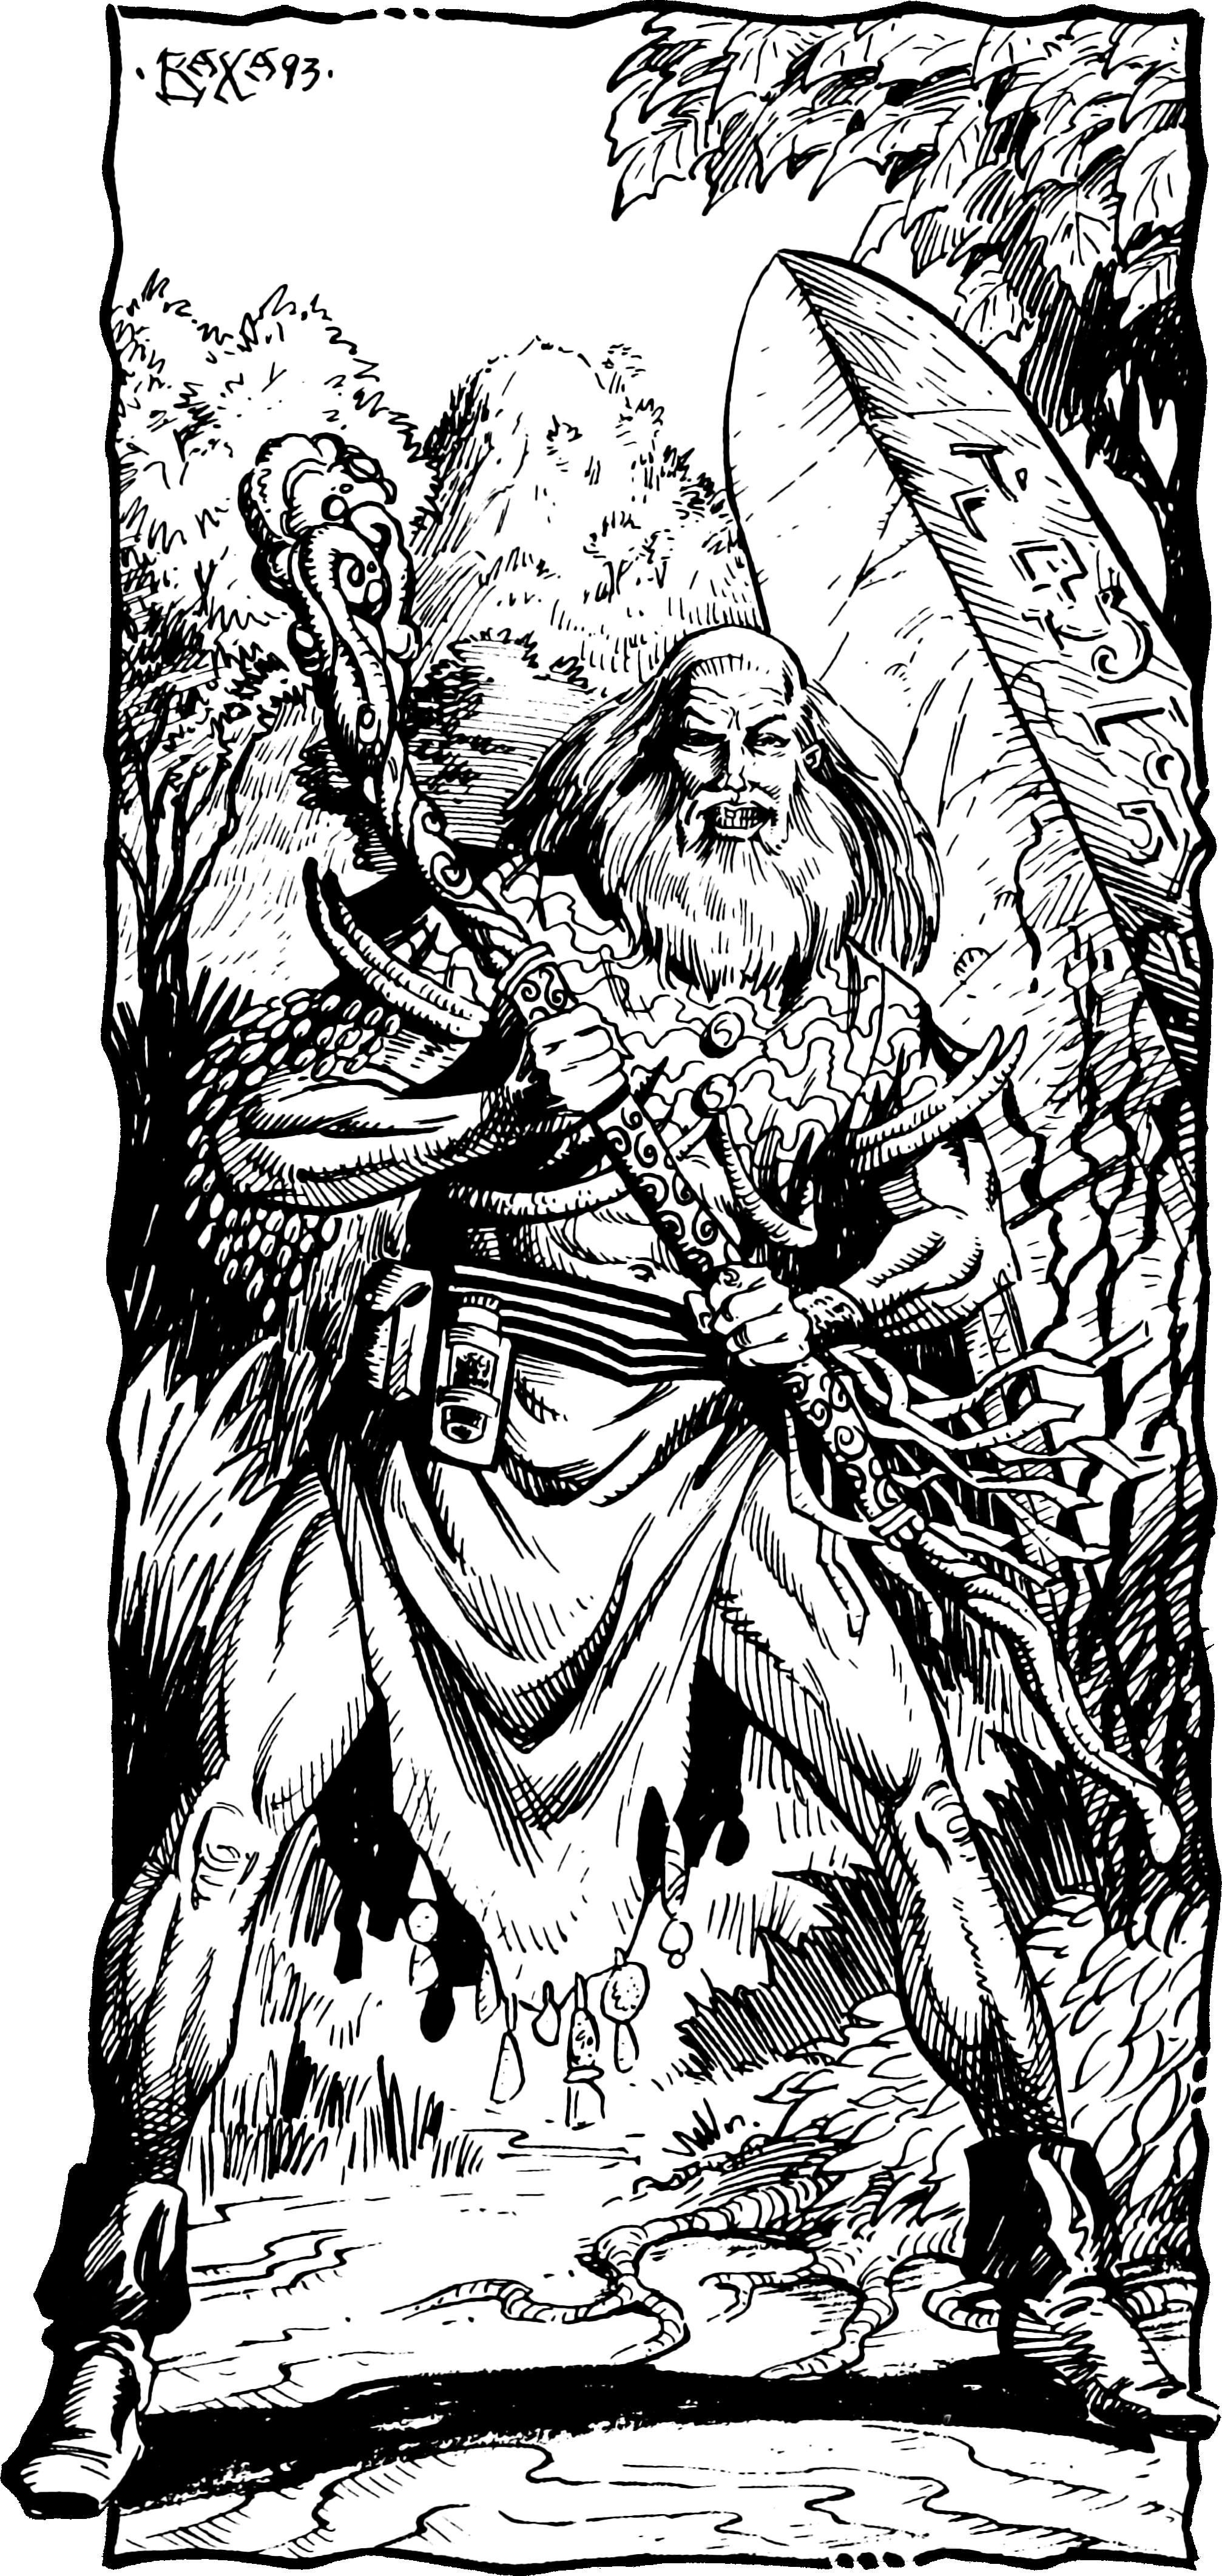
\includegraphics[width=\columnwidth]{images/druid-2.png}
\WOTC
\end{figure}

\subsubsection{Class Features}

\textbf{Weapon and Armor Proficiency:} Druids are proficient with the following weapons: alak, blowgun, club, dagger, dart, quarterstaff, scimitar, sickle, shortspear, sling, and spear. They are also proficient with all natural attacks (claw, bite, and so forth) of any form they assume with wild shape.

Druids are proficient with light and medium armor but are prohibited from wearing metal armor; thus, they may wear only padded, leather, or hide armor. (A druid may also wear wooden armor that has been altered by the ironwood spell so that it functions as though it were steel. See the ironwood spell description) Druids are proficient with shields (except tower shields) but must use only wooden ones.

A druid who wears prohibited armor or carries a prohibited shield is unable to cast druid spells or use any of her supernatural or spell-like class abilities while doing so and for 24 hours thereafter.

\textbf{Spells:} A druid casts divine spells, which are drawn from the druid spell list. Her alignment may restrict her from casting certain spells opposed to her moral or ethical beliefs; see Chaotic, Evil, Good, and Lawful Spells, below. A druid must choose and prepare her spells in advance (see below).

To prepare or cast a spell, the druid must have a Wisdom score equal to at least 10 + the spell level. The Difficulty Class for a saving throw against a druid's spell is 10 + the spell level + the druid's Wisdom modifier.

Like other spellcasters, a druid can cast only a certain number of spells of each spell level per day. Her base daily spell allotment is given on \tabref{The Druid}. In addition, she receives bonus spells per day if she has a high Wisdom score. She does not have access to any domain spells or granted powers, as a cleric does.

A druid prepares and casts spells the way a cleric does, though she cannot lose a prepared spell to cast a cure spell in its place (but see Spontaneous Casting, below). A druid may prepare and cast any spell on the druid spell list, provided that she can cast spells of  that level, but she must choose which spells to prepare during her daily meditation.

\textbf{Spontaneous Casting:} A druid can channel stored spell energy into summoning spells that she hasn't prepared ahead of time. She can ``lose'' a prepared spell in order to cast any summon nature's ally spell of the same level or lower.

\textbf{Chaotic, Evil, Good, and Lawful Spells:} A druid can't cast spells of an alignment opposed to her own. Spells associated with particular alignments are indicated by the chaos, evil, good, and law descriptors in their spell descriptions.

\textbf{Bonus Languages:} A druid's bonus language options include Sylvan, the language of woodland creatures. This choice is in addition to the bonus languages available to the character because of her race.

A druid also knows Druidic, a secret language known only to druids, which she learns upon becoming a 1st-level druid. Druidic is a free language for a druid; that is, she knows it in addition to her regular allotment of languages and it doesn't take up a language slot. Druids are forbidden to teach this language to nondruids. Druidic has its own alphabet.

% \textbf{Animal Companion (Ex):} A druid may begin play with an animal companion selected from the following list: lesser boneclaw, carru, dire rat, eagle, erdlu, jankx, jhakar, kes'trekel, kivit, owl, snake (Small or Medium viper). If the DM's campaign takes place wholly or partly in a silt environment, the DM may add silt spawn to the druid's list of options. This animal is a loyal companion that accompanies the druid on her adventures as appropriate for its kind. 

% A 1st-level druid's companion is completely typical for its kind except as noted below. As a druid advances in level, the animal's power increases as shown on the table. If a druid releases her companion from service, she may gain a new one by performing a ceremony requiring 24 uninterrupted hours of prayer. This ceremony can also replace an animal companion that has perished.

% A druid of 4th level or higher may select from alternative lists of animals. Should she select an animal companion from one of these alternative lists, the creature gains abilities as if the character's druid level were lower than it actually is. Subtract the value indicated in the appropriate list header from the character's druid level and compare the result with the druid level entry on the table to determine the animal companion's powers. (If this adjustment would reduce the druid's effective level to 0 or lower, she can't have that animal as a companion.)

\textbf{Nature Sense (Ex):} A druid gains a +2 bonus on \skill{Knowledge} (nature) and \skill{Survival} checks.

\textbf{Wild Empathy (Ex):} A druid can improve the attitude of an animal. This ability functions just like a \skill{Diplomacy} check made to improve the attitude of a person. The druid rolls 1d20 and adds her druid level and her Charisma modifier to determine the wild empathy check result. The typical domestic animal has a starting attitude of indifferent, while wild animals are usually unfriendly.

To use wild empathy, the druid and the animal must be able to study each other, which means that they must be within 9 meters of one another under normal conditions. Generally, influencing an animal in this way takes 1 minute but, as with influencing people, it might take more or less time.

A druid can also use this ability to influence a magical beast with an Intelligence score of 1 or 2, but she takes a $-4$ penalty on the check.

\textbf{Woodland Stride (Ex):} Starting at 2nd level, a druid may move through any sort of undergrowth (such as natural thorns, briars, overgrown areas, and similar terrain) at her normal speed and without taking damage or suffering any other impairment. However, thorns, briars, and overgrown areas that have been magically manipulated to impede motion still affect her.

\textbf{Trackless Step (Ex):} Starting at 3rd level, a druid leaves no trail in natural surroundings and cannot be tracked. She may choose to leave a trail if so desired.

\textbf{Nature's Speech (Su):} Starting at 4th level, a druid become able to speak with animals everywhere, as if under the effects of the \spell{speak with animals} spell.

\textbf{Wild Shape (Su):} At 5th level, a druid gains the ability to turn herself into any Small or Medium animal and back again once per day. Her options for new forms include all creatures with the animal type. This ability functions like the alternate form special ability, except as noted here. The effect lasts for 1 hour per druid level, or until she changes back. Changing form (to animal or back) is a standard action and doesn't provoke an attack of opportunity. Each time you use wild shape, you regain lost hit points as if you had rested for a night.

Any gear worn or carried by the druid melds into the new form and becomes nonfunctional. When the druid reverts to her true form, any objects previously melded into the new form reappear in the same location on her body that they previously occupied and are once again functional. Any new items worn in the assumed form fall off and land at the druid's feet.

The form chosen must be that of an animal the druid is familiar with.

A druid loses her ability to speak while in animal form because she is limited to the sounds that a normal, untrained animal can make, but she can communicate normally with other animals of the same general grouping as her new form. (The normal sound a wild parrot makes is a squawk, so changing to this form does not permit speech.)

A druid can use this ability more times per day at 6th and every three levels thereafter (9th, 12th, 15th, and 18th level). In addition, she gains the ability to take the shape of a Large animal at 9th level, a Tiny animal at 13th level, and a Huge animal at 17th level. The new form's Hit Dice can't exceed the character's druid level.

At 12th level, a druid becomes able to use wild shape to change into a plant creature with the same size restrictions as for animal forms. (A druid can't use this ability to take the form of a plant that isn't a creature.)

At 18th level, a druid becomes able to use wild shape to change into a vermin with the same size restriction as for animal forms. This transformation uses two wild shape daily uses. In addition to the normal effects of wild shape, the druid gains all the vermin's special qualities. (A druid maintains her Intelligence score and does not gain the vermin traits.)

% At 18th level, a druid becomes able to use wild shape to change into an elemental (air, earth, fire, or water) with the same size restriction as for animal forms. This transformation uses two wild shape daily uses. In addition to the normal effects of wild shape, the druid gains all the elemental's extraordinary, supernatural, and spell-like abilities. She also gains the elemental's feats for as long as she maintains the wild shape, but she retains her own creature type.

% At 18th level, a druid becomes able to assume elemental form twice per day, and at 20th level she can do so three times per day. At 20th level, a druid may use this wild shape ability to change into a Huge elemental.

\textbf{Venom Immunity (Ex):} At 8th level, a druid gains immunity to all poisons.

\textbf{A Thousand Faces (Su):} At 14th level, a druid gains the ability to change her appearance at will, as if using the \spell{disguise self} spell, but only while in her normal form. This affects the druid's body but not her possessions. It is not an illusory effect, but a minor physical alteration of the druid's appearance, within the limits described for the spell.

\textbf{Timeless Body (Ex):} After attaining 16th level, a druid no longer takes ability score penalties for aging and cannot be magically aged. Any penalties she may have already incurred, however, remain in place. Bonuses still accrue, and the druid still dies of old age when her time is up.

\subsubsection{Ex-Druids}
A druid who ceases to revere nature, changes to a prohibited alignment, or teaches the Druidic language to a nondruid loses all spells and druid abilities (not including weapon, armor, and shield proficiencies). She cannot thereafter gain levels as a druid until she atones (see the \spell{atonement} spell description).
% A druid who ceases to revere nature, changes to a prohibited alignment, or teaches the Druidic language to a nondruid loses all spells and druid abilities (including her animal companion, but not including weapon, armor, and shield proficiencies). She cannot thereafter gain levels as a druid until she atones (see the \spell{atonement} spell description).

% \subsubsection{The Druid's Animal Companion}
% A druid's animal companion is different from a normal animal of its kind in many ways. A druid's animal companion is superior to a normal animal of its kind and has special powers, as described below.

% \begin{figure}[b!]
% \centering
% 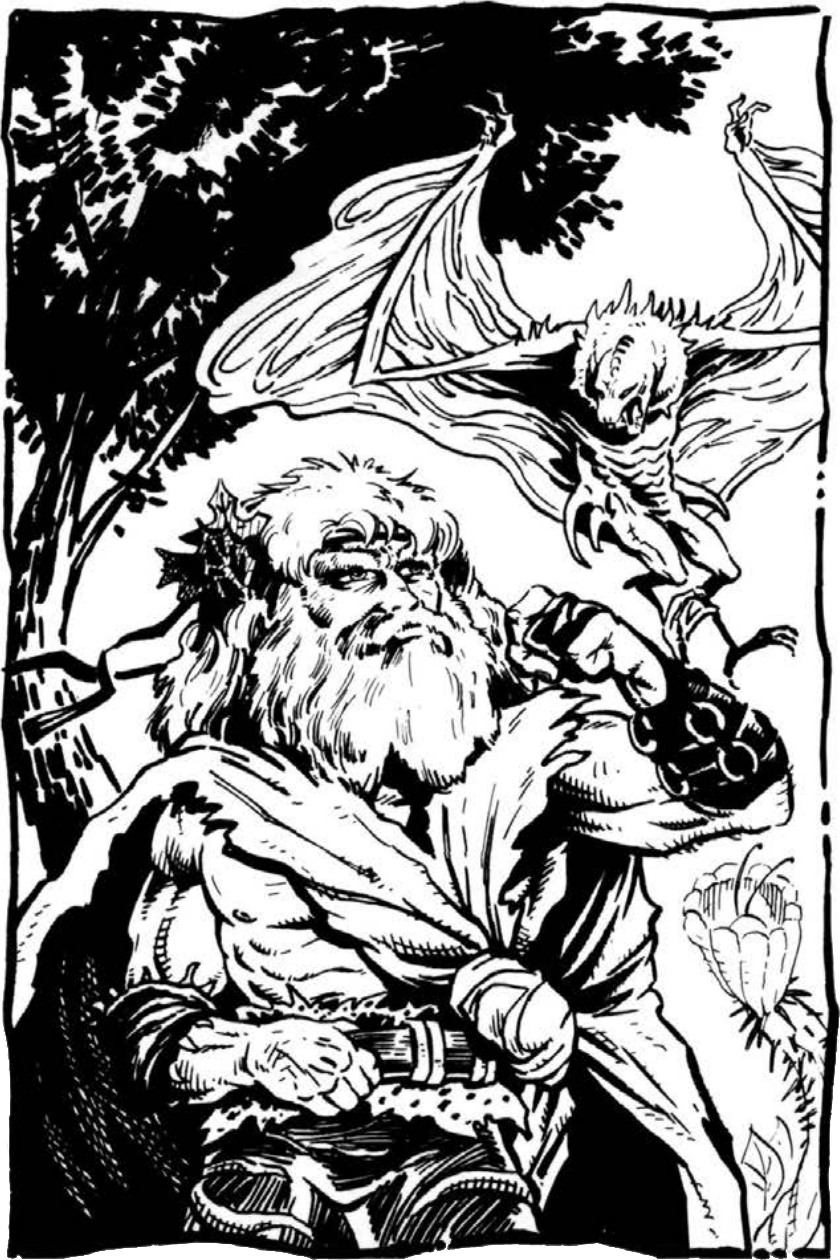
\includegraphics[width=\columnwidth]{images/druid-1.png}
% \WOTC
% \end{figure}

% \Table{}{l Z{.5cm} Z{.8cm} Z{.8cm} Z{.7cm} X}{\tableheader Class Level & \tableheader Bonus HD & \tableheader Natural Armor Adj. &\tableheader  Str/Dex Adj. &\tableheader  Bonus Tricks &\tableheader  Special\\
% 1st--2nd &&&& 1 & Link, share spells\\
% 3rd--5th & +2 & +2 & +1 & 2 & Evasion\\
% 6th--8th & +4 & +4 & +2 & 3 & Devotion\\
% 9th--11th & +6 & +6 & +3 & 4 & Multiattack\\
% 12th--14th & +8 & +8 & +4 & 5 &\\
% 15th--17th & +10 & +10 & +5 & 6 & Improved evasion\\
% 18th--20th & +12 & +12 & +6 & 7 &}

% \textbf{Animal Companion Basics:} Use the base statistics for a creature of the companion's kind, but make the following changes.

% \textbf{Class Level:} The character's druid level. The druid's class levels stack with levels of any other classes that are entitled to an animal companion for the purpose of determining the companion's abilities and the alternative lists available to the character.

% \textbf{Bonus HD:} Extra eight-sided (d8) Hit Dice, each of which gains a Constitution modifier, as normal. Remember that extra Hit Dice improve the animal companion's base attack and base save bonuses. An animal companion's base attack bonus is the same as that of a druid of a level equal to the animal's HD. An animal companion has good Fortitude and Reflex saves (treat it as a character whose level equals the animal's HD). An animal companion gains additional skill points and feats for bonus HD as normal for advancing a monster's Hit Dice.

% \textbf{Natural Armor Adj.:} The number noted here is an improvement to the animal companion's existing natural armor bonus.

% \textbf{Str/Dex Adj.:} Add this value to the animal companion's Strength and Dexterity scores.

% \textbf{Bonus Tricks:} The value given in this column is the total number of ``bonus'' tricks that the animal knows in addition to any that the druid might choose to teach it (see the \skill{Handle Animal} skill). These bonus tricks don't require any training time or \skill{Handle Animal} checks, and they don't count against the normal limit of tricks known by the animal. The druid selects these bonus tricks, and once selected, they can't be changed.

% \textbf{Link (Ex):} A druid can handle her animal companion as a free action, or push it as a move action, even if she doesn't have any ranks in the \skill{Handle Animal} skill. The druid gains a +4 circumstance bonus on all wild empathy checks and \skill{Handle Animal} checks made regarding an animal companion.

% \textbf{Share Spells (Ex):} At the druid's option, she may have any spell (but not any spell-like ability) she casts upon herself also affect her animal companion. The animal companion must be within 1.5 meter of her at the time of casting to receive the benefit. If the spell or effect has a duration other than instantaneous, it stops affecting the animal companion if the companion moves farther than 1.5 meter away and will not affect the animal again, even if it returns to the druid before the duration expires.

% Additionally, the druid may cast a spell with a target of ``You'' on her animal companion (as a touch range spell) instead of on herself. A druid and her animal companion can share spells even if the spells normally do not affect creatures of the companion's type (animal).

% \textbf{Evasion (Ex):} If an animal companion is subjected to an attack that normally allows a Reflex saving throw for half damage, it takes no damage if it makes a successful saving throw.

% \textbf{Devotion (Ex):} An animal companion gains a +4 morale bonus on Will saves against enchantment spells and effects.

% \textbf{Multiattack:} An animal companion gains \feat{Multiattack} as a bonus feat if it has three or more natural attacks and does not already have that feat. If it does not have the requisite three or more natural attacks, the animal companion instead gains a second attack with its primary natural weapon, albeit at a $-5$ penalty.

% \textbf{Improved Evasion (Ex):} When subjected to an attack that normally allows a Reflex saving throw for half damage, an animal companion takes no damage if it makes a successful saving throw and only half damage if the saving throw fails.

% \subsubsection{Alternative Animal Companions}
% A druid of sufficiently high level can select her animal companion from one of the following lists, applying the indicated adjustment to the druid's level (in parentheses) for purposes of determining the companion's characteristics and special abilities.

% Some animals are only available in certain environments. The animals available only in an aquatic environment, such as the Last Sea, are marked with $\dagger$. The animals available only in a silt environment, such as the Sea of Silt, are marked with $\diamond$.

% \Table{}{X X}{
% \multicolumn{2}{c}{\tableheader\footnotesize 4th Level or Higher (Level $-3$)}\\
% Carru, bull (6HD) & Leopard \\
% Cheetah & Lizard, giant \\
% Crodlu & Lizard, monitor\\
% Crodlu, heavy & Rasclinn\\
% Dire bat & Athasian shark$^\dagger$\\
% Erdland & Snake, constrictor\\
% Jhakar, Medium (6HD) & Snake, viper (Large)\\
% Kluzd & }

% \Table{}{X X}{
% \multicolumn{2}{c}{\tableheader\footnotesize 7th Level or Higher (Level $-6$)}\\
% Crodlu, heavy warmount & Puddingfish$^\dagger$ \\
% Inix & Lion\\
% Kalin & Lizard, subterranean\\
% Kluzd (7HD) & Snake, viper (Huge)\\
% Lirr & Takis\\
% Pterrax & Tiger}

% \Table{}{X X}{
% \multicolumn{2}{c}{\tableheader\footnotesize 10th Level or Higher (Level $-9$)}\\
% Cha'thrang & Lizard, minotaur\\
% Dire lion & Athasian shark (Huge)$^\dagger$ \\
% Hatori & Snake, giant constrictor}

% \Table{}{X X}{
% \multicolumn{2}{c}{\tableheader\footnotesize 13th Level or Higher (Level $-12$)}\\
% Lirr, large (11HD) & Athasian sloth\\
% Ruktoi$^\diamond$ & }

% \Table{}{X X}{
% \multicolumn{2}{c}{\tableheader\footnotesize 16th Level or Higher (Level $-15$)}\\
% Dire Athasian shark$^\dagger$ & Silt Horror, white$^\diamond$\\
% Dire tiger&Slimahacc\\
% Hatori, gargantuan (17HD) &}

\subsection{Playing a Druid}
You are a humanoid servant devoted to Athas and all of its elements equally. As a guardian, tender, warrior, and sometimes assassin, you further the cause of nature and help to make Athas verdant again.

You, like nature itself is neutral. You see the balance of all things. You know that every living creature is part of the food chain, and birth and death are the natural order of life. This is one of the reasons druids harbor such intense hatred for the defilers. Their magic of decay lies outside the normal cycle of life. Matter should not be destroyed, but converted to a form that will eventually return to the earth. Defiling magic destroys that which should never be destroyed, and its practice is an abomination to druids.

\subsubsection{Religion}
A druid is an individual who has devoted themselves to the balance of nature on Athas, and in particular someone who has sought out or been chosen by one of the few living spirits left in the barren land, protecting and nurturing them and the natural balance they represent.

Individual druids do not necessarily recognize one another as kin or as brothers in a religion; each conducts their affairs as they see fit in their quest to restore the balance of nature and protect their spirit's lands. Most druids recognize the various spirits as a manifestation of Athas itself, though some few more primitive or uncultured individuals or groups may believe the spirit to be a god and treat it as such.

\subsubsection{Other Classes}
Druids get along with most classes, though they despise wizards. Magic is the cause of Athas' current state, so say the druids, and while they may tolerate preservers for a short while, defilers are slain on sight. Templars are usually not welcomed by druids, as the templar is responsible for a city that encroaches on nature, and templars serve the sorcerer-kings, Athas' most powerful magic users. Elemental clerics are well received by druids, as they often share the same goals. Druids are usually at odds with paraelemental clerics, though. The paraelement proliferation on Athas is usually at the land's expense, destroying what the druid tries to accomplish.

Rangers are probably the druid's best allies. They often share the same goals, and the druid may even call upon the ranger for help in controlling a species that has become problematic or detrimental to an area. However, the ranger and the druid may sometimes be at odds, if the ranger is determined to eradicate his favored enemy while the druid seeks to protect that particular species.

\subsubsection{Combat}
Your ability to summon creatures and to turn into them is your primary weapons. Consider using them to aid your companions in flanking maneuvers, or better yet to harass enemy spellcasters (many of whom are easy to hit), especially if they are defilers. Few foes are prepared for an opponent who can call such potent beings to service, so you've also got the advantage of surprise.

Though somewhat skilled at both combat and spellcasting, you are more suited to guerrilla warfare---tracking enemies to their lair ambushing them while they sleep, or engaging in other sue surreptitious tactics. With woodland stride and trackless step, you can usually escape through the wilderness before your enemies know what hit them.

\subsubsection{Advancement}

You profit most from remaining a druid thought your advancement, so that %your animal companion and 
wild shape continue to improve as you gain levels. If you do multiclass, a level of barbarian is an excellent choice; the benefits it grants to combat and movement regardless of when you take that 1st level.

During their time of wandering, a young druid learns about the world, its ecology, the balance of nature and the ways of its creatures. After a few years of peregrination, most druids decide to settle in order to watch over a specific patch of land lands, watching over them and protecting them, and straighten their bond with a Spirit of the Land. Such druids become \class{Grove Masters}.

\subsection{Starting Packages}
\subsubsection{The Beastmaster}

Half-Elf Druid

\textbf{Ability Scores:} Str 10, Dex 15, Con 12, Int 8, Wis 15, Cha 12.

\textbf{Skills:} \skill{Handle Animal}, \skill{Hide}, \skill{Survival}.

\textbf{Languages:} Common, Elven.

\textbf{Feat:} \feat{Animal Affinity}.

\textbf{Weapons:} Longspear (1d8/$\times$3)

Sling with 20 bullets (1d4, 15 m).

\textbf{Armor:} Hide (+3 AC).

\textbf{Gear:} Spell component pouch, standard adventurer's kit, 20 cp.

\textbf{Class Features:} Jankx animal companion.

\textbf{Spells Prepared:} 1st---\spell{cure light wounds}, \spell{speak with animals}; 0---\spell{cure minor wounds} (2), \spell{defiler scent}.

\subsubsection{The Defiler Hunter}

Human Druid

\textbf{Ability Scores:} Str 13, Dex 14, Con 12, Int 10, Wis 15, Cha 8.

\textbf{Skills:} \skill{Concentration}, \skill{Hide}, \skill{Listen}, \skill{Move Silently}, \skill{Spot}, \skill{Survival}.

\textbf{Languages:} Common

\textbf{Feat:} \feat{Defender of the Land}, \feat{Track}.

\textbf{Weapons:} Spear (1d8/$\times$3, 6m)

Sling with 20 bullets (1d4, 15 m).

\textbf{Armor:} Hide (+3 AC).

\textbf{Gear:} Spell component pouch, standard adventurer's kit, 20 cp.

\textbf{Class Features:} Jhakar animal companion.

\textbf{Spells Prepared:} 1st---\spell{backlash}, \spell{longstrider};\hskip10pt 0---\spell{cure minor wounds}, \spell{defiler scent} (2).

\subsubsection{The Warden}

Pterran Druid

\textbf{Ability Scores:} Str 8, Dex 11, Con 14, Int 10, Wis 17, Cha 14.

\textbf{Skills:} \skill{Hide}, \skill{Knowledge} (nature), \skill{Move Silently}, \skill{Spot}, \skill{Survival}.

\textbf{Languages:} Saurian.

\textbf{Feat:} \feat{Spell Focus} (conjuration).

\textbf{Weapons:} Alak (1d6/$\times$3)

Blowgun with 20 needles (1, 3 m).

\textbf{Armor:} Leather (+2 AC), light wooden shield (+1 AC).

\textbf{Gear:} Spell component pouch, standard adventurer's kit, 20 cp.

\textbf{Class Features:} Lesser boneclaw animal companion.

\textbf{Spells Prepared:} 1st---\spell{entangle}, \spell{plant renewal}; 0---\spell{defiler scent}, \spell{detect magic}, \spell{nurturing seeds}.

\subsection{Druids on Athas}
\Quote{The druids are no longer hunted in force by the sorcerer-kings. The kings believe there simply aren't enough left to threaten them. But the templars, and even some elves I know, have been well rewarded for delivering the heads of wasteland druids.}{Jurgan, Urikite earth cleric}

Perhaps the only thing rarer to see in Athas than a wizard is a druid. After centuries of persecution, they were forced to either die in the hands of the agents of the sorcerer-monarchs, or to watch their beloved land wither and die before their eyes.

Because of that, druids are usually loners and avert to social interaction. They live off the land, within the land, and they have sacrificed their entire lives for the land, very little besides it occupies the mind of a druid.

\subsubsection{Daily Life}

A druid adventures to learn about Athas, to protect nature, and to further his own aims. Druids usually spend their days in contemplation of nature, and tending their lands; one may watch over a particular stretch of open desert, another may protect a belt of scrub grass within it, while still another might watch over a small oasis that borders on both, always hidden and always watching.

The Athasian druid is a wanderer who hunts down a powerful defiler that has despoiled the wastes, or a visionary who tends the land and teaches the local population how to live in harmony with their surroundings. The Athasian druid fights for an almost lost cause, and it matters not if that cause is revenge himself against those who destroyed his land and friends or a ceaseless desire to bring green and hope to Athas.

\subsubsection{Notables}

Druids very rarely become famous, since they usually avoid social interaction combined the fact that it might put their lives at risk since usually sorcerer-kings and defiler usually put a reward for the head of a notorious or troublesome druid. A legend claim that Mearedes the druidess came to the island of Shault when its forest was all but dead and she managed to nurture it back to its vibrant health.

\subsubsection{Organizations}

Ever since the Eradication, an anti-druidic jihad led by sorcerer-kings more than 1,500 years ago, no specific druidic organization exists, although some form temporary alliances with Veiled Alliance members from time to time. Legends say that the druids who remained after the Eradication gathered on a high mesa somewhere in the northern Tablelands. It was there they decided that they should scatter to the most remote reaches and farthest regions of Athas, there to bide their time, waiting for the day when they were powerful enough to challenge the sorcerer-kings again. This was a long time ago, and the druids have yet to return to the cities of the defilers. Some say that they will never return and that their seclusion and isolation have destroyed whatever power they once wielded as a circle. Others say that the druid's long wait is indicative of their cunning, and that their plan is to insure that the next confrontation with the kings won't end in defeat.

\subsubsection{NPC Reactions}

Druids are natural loners, and usually avoid social interactions unless they have to. In such cases, those who are directly benefited from the druid's work of tending the land begin two steps nearer helpful, while defilers and evil paraelemental clerics begin two steps nearer hostile.

\subsubsection{Druid Lore}

Characters with ranks in \skill{Knowledge} (nature) can research druids to learn more about them. When a character makes a skill check, read or paraphrase the following, including the information from lower DCs.

\textbf{DC 10:} Druids devote themselves to the land, drawing off their power straight from Athas itself.

\textbf{DC 15:} Druids from a mystical connection to mysterious beings known as Spirits of the Land. They hate all defilers and those who abuse the land.

\textbf{DC 20:} Druids are masters of the forces of nature, being able to transform into the creatures that dwell in their lands, and some even learn to counter the destruction of defilement.

\Class{Fighter}
{Any wastelander can pick up a bone and call it a club, but try pitting fifty of those against one dozen trained soldiers, and maybe you'll have an even match.}{Nikolos, human fighter}

From the small forts in sandy wastes of Athas to the guards of the merchant houses in the city-states, fighters are Athas' most common sight. Whether it is as mercenaries for the sorcerer-kings or as hired guards protecting the wealth of the nobility, fighters can be found everywhere in the Tablelands. Athas' fighters are trained to fight in small groups or huge units. Those that have proven themselves become the commanders in the city-states' armies, commanding hundreds or even thousands of men into war.

\subsection{Making a Fighter}
Fighters receive the best allotment of fighting skills and abilities. They learn the use of most weapons, the best armors and shields, as well as gaining special abilities to use with these weapons and armor.

Some fighters specialize in using a single weapon, and become masters at its use and deadliness. Other fighters will prefer more rounded skills, learning to shoot from far with bows and arrows, or nets or spears. Regardless, the fighter is to be feared.

\textbf{Races:} All of Athas' races can become fighters. Humans are usually the most numerous, though, since they are the most numerous of the races of the Tablelands. Dwarves make good fighters, even though they are smaller than most races; their inborn toughness and great strength more than makes up for their smaller stature. The half-giants are also seen very often as fighters, since their great strength and size are perfect for the job. Muls, with the inherited traits of both humans and dwarves, are also great fighters. Elves, with their long legs and frail constitution, are not often seen as fighters. Athas' intelligent insects, the Thri-kreen, make excellent warriors, with their four arms and the fact they do not need to sleep. Many of the savage races of the Tablelands are fighters, although most become rangers in order to survive.

\textbf{Alignment:} Fighters come from all walks of life, and can be of any alignment. Good fighters are usually seen as the protectors of small villagers or are part of renegade slave tribes, helping their tribe to survive in the harsh desert. Or they can be found as a dwarf perhaps, whose focus it is to guard his fellows. Evil fighters are often part of mercenary bands or under the control of a sorcerer-king; these beings often fight for power and money. Evil fighters can also be found as the rulers of small forts, guarding their oasis and exacting a hefty toll for its use.

\Figure{t}{images/fighter-3.png}

\MiniWarriorTable{The Fighter}{
1st  & +1             & +2  & +0 & +0 & Bonus feat \\
2nd  & +2             & +3  & +0 & +0 & Bonus feat \\
3rd  & +3             & +3  & +1 & +1 &  \\
4th  & +4             & +4  & +1 & +1 & Bonus feat \\
5th  & +5             & +4  & +1 & +1 & Martial prowess \\
6th  & +6/+1          & +5  & +2 & +2 & Bonus feat \\
7th  & +7/+2          & +5  & +2 & +2 & Martial prowess \\
8th  & +8/+3          & +6  & +2 & +2 & Bonus feat \\
9th  & +9/+4          & +6  & +3 & +3 & Martial prowess \\
10th & +10/+5         & +7  & +3 & +3 & Bonus feat \\
11th & +11/+6/+1      & +7  & +3 & +3 & Martial prowess \\
12th & +12/+7/+2      & +8  & +4 & +4 & Bonus feat \\
13th & +13/+8/+3      & +8  & +4 & +4 & Martial prowess \\
14th & +14/+9/+4      & +9  & +4 & +4 & Bonus feat \\
15th & +15/+10/+5     & +9  & +5 & +5 & Martial prowess \\
16th & +16/+11/+6/+1  & +10 & +5 & +5 & Bonus feat \\
17th & +17/+12/+7/+2  & +10 & +5 & +5 & Martial prowess \\
18th & +18/+13/+8/+3  & +11 & +6 & +6 & Bonus feat \\
19th & +19/+14/+9/+4  & +11 & +6 & +6 & Martial prowess \\
20th & +20/+15/+10/+5 & +12 & +6 & +6 & Bonus feat \\
}

\subsection{Game Rule Information}
\textbf{Hit Die:} d10.

\subsubsection{Class Skills}
\skill{Autohypnosis} (Wis), \skill{Climb} (Str), \skill{Craft} (Int), \skill{Handle Animal} (Cha), \skill{Intimidate} (Cha), \skill{Jump} (Str), \skill{Knowledge} (warcraft) (Int), \skill{Ride} (Dex), and \skill{Spot} (Wis).

\textbf{Skill Points per Level:} 4 + Int modifier ($\times4$ at 1st level).

\subsubsection{Class Features}
\textbf{Weapon and Armor Proficiency:} A fighter is proficient with all simple and martial weapons and with all armor (heavy, medium, and light) and shields (including tower shields).

\textbf{Bonus Feats:} At 1st level, a fighter gets a bonus combat-oriented feat in addition to the feat that any 1st-level character gets and the bonus feat granted to a human character. The fighter gains an additional bonus feat at 2nd level and every two fighter levels thereafter (4th, 6th, 8th, 10th, 12th, 14th, 16th, 18th, and 20th). These bonus feats must be drawn from the feats noted as fighter bonus feats. A fighter must still meet all prerequisites for a bonus feat, including ability score and base attack bonus minimums.

These bonus feats are in addition to the feat that a character of any class gets from advancing levels. A fighter is not limited to the list of fighter bonus feats when choosing these feats.

\textbf{Martial Prowess:} At 5th level and every two levels thereafter, a fighter improves his repertoire with new techniques. He may choose one of the following options.

\textit{Active Defense (Ex):} A fighter gains a dodge bonus to AC equal to \onequarter his fighter levels when wielding a shield and fighting defensively or using the \feat{Combat Expertise} feat. When using total defense, this bonus increases to \onehalf his fighter levels.

\textit{Aim (Ex):} A fighter can take full-round action to make a \skill{Spot} check to improve his next attack against a specific foe. DC is equal to his target's AC. His next attack against the target ignore armor bonus and natural armor bonus. This attack must be made within a number of rounds equal to \onequarter his fighter levels.

\Figure*{t}{images/battle-1.png}

\textit{Ambidextrous (Ex):} A fighter may add his full Strength modifier to his off-hand weapon damage, instead of \onehalf his Strength bonus.

\textit{Bravery (Ex):} A fighter with this ability gains a bonus equal to \onehalf his fighter levels on Will saves against mind-affecting abilities.

\textit{Close Combat Shot (Ex):} A fighter can attack with a ranged weapon while in a threatened square and not provoke an attack of opportunity.

\textit{Commanding Strike (Ex):} A fighter may forgo his attack with the lowest base attack bonus in a total attack to create an opening for an ally. The designated ally may use one of his attacks of opportunity to strike a foe. The ally may use ranged attacks---this is an exception for the rules for attacks of opportunity.

\textit{Coordinate Allies (Ex):} A fighter can use a full-round action to identify and apply an effective tactic for his allies. Each creature to be affected must be able to see and hear him, and able to pay attention to him. To coordinate, the fighter must make a \skill{Knowledge} (warcraft) check with a DC equal to 15 + the number of allies affected. If the check succeeds, all affected allies gain a competence bonus on attack rolls or a dodge bonus to AC equal to \onequarter his fighter levels. He chooses which of the two benefits to impart and must impart the same benefit to all affected allies. The benefits last for 1 round. The fighter cannot use this ability on himself.

\textit{Crossbowman (Ex):} Whenever a fighter attacks with a crossbow as a readied action, his target is denied its Dexterity bonus to its AC.

\textit{Defensive Tactics (Ex):} A fighter may use a move action to coordinate his allies to a defensive maneuver. Each creature to be affected must be able to see and hear him, and able to pay attention to him. To coordinate, the fighter must make a \skill{Knowledge} (warcraft) check with a DC equal to 10 + the number of allies affected. If the check succeeds, all affected allies gain a moral bonus to AC against attacks of opportunity equal to \onequarter his fighter levels. The benefits last for 1 round.

\textit{Double Opportunity (Ex):} When a fighter makes an attack of opportunity, he may attack once with both his primary and secondary weapons. The penalties for attacking with two weapons apply normally. The fighter must be at least 11th level to select this technique.

\textit{Flanking Tactics (Ex):} A fighter may use a move action to coordinate his allies to a flanking maneuver against a target. Each creature to be affected must be able to see and hear him, and able to pay attention to him. To coordinate, the fighter must make a \skill{Knowledge} (warcraft) check with a DC equal to the target's Base Attack Bonus. If the check succeeds, all affected allies gain a competence bonus on damage rolls equal to \onequarter his fighter levels when they flank the target. The benefits last for 1 round. The fighter cannot use this ability on himself.

\textit{Harden Resolve (Ex):} A fighter may use a standard action to improve his allies' morale. Each creature to be affected must be able to see and hear him, and able to pay attention to him. To coordinate, the fighter must make a \skill{Knowledge} (warcraft) check with a DC equal to 25 + 2 for each ally affected. If the check succeeds, all affected allies gain damage reduction equal to \onequarter his fighter levels. If an ally already has damage reduction, it improves by the same amount. The benefits last for 1 round. A fighter must be at least 11th level to select this technique.

\textit{Hawkeye (Ex):} Whenever a fighter isn't flat-footed, he has advantage on \skill{Spot} checks.

\textit{Lead the Charge (Ex):} A fighter may make a \skill{Knowledge} (warcraft) check during a charge against one specific foe. The check DC is equal to 20 + the number of allies affected. If the check succeeds, all affected allies that charge the same foe gain a competence bonus on attack and damage rolls equal to \onequarter his fighter levels. The benefits last for 1 round.

\textit{Leadership:} A fighter may gain the \feat{Leadership} feat as a bonus feat.

\textit{Maneuvering Attack (Ex):} A fighter may forgo his attack with the lowest base attack bonus in a total attack to maneuver one of his comrades into a more advantageous position. The fighter chooses a friendly creature that can see and hear him. That creature can use an immediate action to move up to half its speed.

\textit{Martial Versatility (Ex):} A fighter can apply any feat he has that affects only one weapon type (such as, \feat{Weapon Focus} or \feat{Rapid Reload}) to any simple weapon. A fighter must be at least 11th level to select this technique.

\textit{Mirror Move (Ex):} A fighter gains \onequarter his fighter levels as an insight bonus to AC when attacked by any weapon with which he has the \feat{Weapon Specialization} feat.

\textit{Overhand Chop (Ex):} When a fighter makes a single attack (with the attack action or a charge) with a two-handed weapon, he adds triple his Strength bonus on damage rolls, instead of 1\onehalf his Strength bonus.

\textit{Phalanx (Ex):} As long as a fighter is wielding a shield, he may use any two-handed polearm or spear as if it was an one-handed weapon. A fighter cannot use this ability with a buckler.

\textit{Pressing Shield (Ex):} A fighter may use his shield to help with his bull rush and overrun attempts. He adds his shield bonus on Strength checks made to push back the defender, and on Strength checks to knock down his opponent. A fighter cannot use this ability with a buckler.

\textit{Quick Aid (Ex):} A fighter may use the aid another action with a full attack. He must use his attack with the highest base attack bonus and roll against AC 20.

\textit{Ready Polearm (Ex):} A fighter can ready any weapon that deals increased damage against charge as an immediate action. A fighter must be at least 11th level to select this technique.

\textit{Second Wind (Ex):} A fighter with this ability can dig his resolve and endurance to find an extra burst of vitality. He can use a standard action to gain a number of temporary hit points equal to his Constitution modifier $\times$ his fighter levels. These hit points last until for the end of the encounter. He can use this ability only once per encounter.

\textit{Shield Another (Ex):} A fighter can use his shield to protect an adjacent ally. When using aid another to grant AC to an ally, he can choose a number to add as penalty to his shield bonus until his next turn. The ally target of the aid another action gains improves their shield bonus by that number. The fighter can't choose a number greater than his shield bonus or his base attack bonus. A fighter cannot use this ability with a buckler.

\textit{Shorten Haft (Ex):} A fighter may threaten adjacent squares when wielding reach weapons.

\textit{Skirmisher (Ex):} Whenever a fighter moves 3 or more meters in his turn, he gains a dodge bonus against ranged attacks equal to \onequarter his fighter.

\textit{Tortoise Style (Ex):} While wielding a shield, the fighter improves his shield bonus by \onequarter his fighter levels. A fighter cannot use this ability with a buckler.

\textit{Two-handed Style (Ex):} When the fighter rolls a 1 or 2 on a damage die for an attack made with a melee weapon wielded with two hands, he can reroll the die and must use the new roll even if the new roll is a 1 or 2. The fighter cannot use this benefit with light weapons.

\textit{Uncanny Dodge (Ex):} A fighter can react to danger before his senses would normally allow his to do so. He retains his Dexterity bonus to AC (if any) even if he is caught flat-footed or struck by an invisible attacker. However, he still loses his Dexterity bonus to AC if immobilized. If a fighter already has uncanny dodge from a different class he automatically gains improved uncanny dodge instead.

\textit{Weapon Training (Ex):} A fighter improves his aptitude in martial weapons. He gains a competence bonus on his attack rolls equal to \onequarter his fighter levels, whenever he is wielding a simple or martial weapon.


\subsection{Playing a Fighter}
Playing an Athasian fighter is not much different than playing one in other settings, the only difference is that the extreme heat makes most armor less than desirable on Athas.

As a fighter, you undertake adventures according to the dictates of your cause, your faith, or your own selfish needs. You might find yourself on the hot, sandy field of battle, charging shoulder to shoulder with peasants and soldiers, raising pitchforks and shields against the defilers of the enemy army.

\subsubsection{Religion}
There are no gods on Athas, but many fighters worship the sorcerer-king of their respective cities as gods. Some fighters pay homage to the elemental forces of the Tablelands, asking their favored element for luck before entering the battlefield.

\subsubsection{Other Classes}
Fighters get along with most other classes. The rangers of the Tablelands often receive the highest of the respect for their ability to survive the wastes. Gladiators and fighters are often at each other's throats, since both share great combat abilities but differ in their methodology; they often try to show how each is better than the other is. Elemental clerics are welcome for their healing abilities as well as the help they can provide in battle.

Fighters are uneasy around wizards; like the rest of the population they distrust magic. Templars are also distrusted, for the same reasons everyone else distrusts templars. Rogues are usually scorned by fighters; they prefer open battle to the rogue's sneaky ways.

\subsubsection{Combat}
Your specific tactics in battle depend on your role in the party and your weapon of choice. However, certain tactics are common to all fighters.

You are generally at the forefront of any battle. Fighting on the front line allows you maximize your combat feats. Furthermore, if opponents focus on you, they cannot injure your allies. As a fighter, you're at your best when you can take on the monster or opponent that deals the most damage.

\subsubsection{Advancement}
When looking at feats to select as you gain levels, you have two basic paths. You can focus on your fighting skills, or you can attempt to expand your capabilities to serve as the party's leader. The former option is best when you are the group's primary combat specialist. If the party includes another fighter or suitable melee character, you can afford to dabble in Charisma-based skills. Although Diplomacy is not a class skill for you, the Field Office feat combined with a few cross-class ranks makes you a serviceable emissary.

When it comes to combat feats, look to ones that improve your ability to deal damage. Feats such as Power Attack, Weapon Focus, and so forth are excellent options to boost your offense. Concentrated Fire, Rotate Lines, Shield Wall, and Spear Wall are excellent feats for army fighters.

Improved Initiative is a critically important feat, since it allows you to act first, move forward and defend or guide your allies. The sooner you find a place in the front line, the longer you can hold back the enemy.


\subsection{Starting Packages}
\subsubsection{The Archer}
Elf Fighter

\textbf{Ability Scores:} Str 15, Dex 16, Con 11, Int 10, Wis 12, Cha 8.

\textbf{Skills:} \skill{Jump}, \skill{Spot} (cc).

\textbf{Languages:} Common, Elven.

\textbf{Feat:} \feat{Point Blank Shot}, \feat{Precise Shot}.

\textbf{Weapons:} Macahuitl (1d8/19-20)

Dagger (1d4/19-20, 3 m)

Longbow with 40 arrows (1d8/$\times$3, 30 m).

\textbf{Armor:} Chitin armor (+4 AC).

\textbf{Gear:} Standard adventurer's kit, 11 cp.

\subsubsection{The Defender}
Dwarf Fighter

\textbf{Ability Scores:} Str 15, Dex 13, Con 16, Int 10, Wis 12, Cha 8.

\textbf{Skills:} \skill{Craft} (weaponsmithing), \skill{Knowledge} (warcraft), \skill{Intimidate}.

\textbf{Languages:} Common, Dwarven.

\textbf{Feat:} \feat{Disciplined}, \feat{Weapon Focus} (dwarven waraxe).

\textbf{Weapons:} Dwarven waraxe (1d10/$\times$3)

Shortbow with 20 arrows (1d6/$\times$3, 18 m).

\textbf{Armor:} Scale mail (+4 AC), heavy wooden shield (+2 AC).

\textbf{Gear:} Standard adventurer's kit, 42 cp.

\subsubsection{The Leader}
Human Fighter

\textbf{Ability Scores:} Str 15, Dex 8, Con 13, Int 10, Wis 12, Cha 14.

\textbf{Skills:} \skill{Diplomacy} (cc), \skill{Knowledge} (warcraft), \skill{Intimidate}.

\textbf{Languages:} Common.

\textbf{Feat:} \feat{Field Officer}, \feat{Inspiring Presence}, \feat{Weapon Focus} (great macahuitl).

\textbf{Weapons:} Great macahuitl (2d6, 19-20)

Shortbow with 20 arrows (1d6/$\times$3, 18).

\textbf{Armor:} Scale mail (+4 AC).

\textbf{Gear:} Standard adventurer's kit, 19 cp.


\subsection{Fighters on Athas}
\Quote[-.em]{Yeah, he was alright with a sword, but he would wet himself every time we walked out onto the sand of the arena. I think it was the crowd... or the goat-headed giant they paired us against. Poor little weed, he never saw that club coming.}{Grek the Grand, talking about his onetime matched pair contest with Slavek Thydor}

Fighters bring clashing weapons, stirring speeches, and mass combat to the campaign. On Athas, the fighter is a trained warrior, a soldier skilled in mass warfare. Every society on Athas maintains an army of fighters to protect itself from attack or to wage wars of plunder and annihilation against its neighbors. Fighters are both the commanders and soldiers in these armies, and at higher levels are experts in both individual and formation combat, leadership, and morale.

\subsubsection{Daily Life}
A fighter adventures to prove his superior skill at arms, to advance the cause of whatever master he might serve, and to further his own aims.

Once he has reached a respectable level of accomplishment, a fighter might take the Leadership feat and start building his own army. As word spreads, less experienced warriors who are eager to fight for the same causes seek him out as the desperate peoples of Athas constantly look for great commanders, warriors who will lead them.

\subsubsection{Notables}
Fighters can notoriety for their deeds, whether triumphs in combat, selfless acts of great honor, or great tyranny. Many an adventurer grew up on stories such as that of the Crimson Legion, and how it managed to defeat Urik's previously undefeated army.

Another legend tells of about the rise and fall of General Zanthiros, the leader of the Balican army who managed to save the city from an onslaught of beast-headed giants more than once, and after losing the elections, left the city with hundreds of soldiers loyal to him and formed a raiding tribe.

\subsubsection{Organizations}
Fighters often band together into small armies or as mercenary groups working for trade houses. These organizations typically have different credos and values, but they allow their members to focus their time on their individual quests.

\subsubsection{NPC Reactions}
Individuals react to fighters based on their previous interactions with other members of the class. A brave fighter meets cold silence and contempt around the Barrier Wastes where evil fighters oppress the populace.

Gladiators usually talk down on fighters, saying that gladiators are the true masters of combat. Fighters usually reply that gladiators are nothing without a crowd looking. Because of that, their initial reaction is one step towards unfriendly than normal.

A fighter who has lived long enough to retire from adventuring typically acquires some position of authority, with commensurate political power, whether as a caravan leader, army general, or ruler of a raiding or slave tribe.

\subsubsection{Fighter Lore}
Characters with ranks in \skill{Knowledge} (warcraft) can research fighters to learn more about them. When a character makes a skill check, read or paraphrase the following, including the information from lower DCs.

\textbf{DC 10:} Fighters may not be as flashy as gladiators in combat, but they surely are more effective in mass combat.

\textbf{DC 15:} Fighters are combat-oriented characters adept at hand-on-hand combat just as well as commanding entire armies.

\textbf{DC 20:} A fighter's mere presence in the battlefield can be enough to inspire his soldiers and weaken the resolve of his enemies.

\Class{Gladiator}
{I might be a slave, but I am famous, I dine well, and my company is that of the finest noble women. Tell me, what do you have that I do not, slave trader---except the freedom to feel miserable?}{Jarek, arena champion}

The arena is the battlefield of the gladiator. From hand-to-hand combat in the mud pits of small forts to the grand games of the city-states, the gladiator is a warrior who fights to the sounds of people cheering his name or cursing his presence. A master of crowd control and the art of prolonged combat, gladiators are trained to fight.

They train to best wild beasts in deadly games for the amusement of the masses. They fight for glory, wealth, prestige and power. They fight to survive. Some are merely slaves, having to fight and perhaps hoping to win a chance to obtain freedom, while some fight willingly for the thrill of combat or the promise of riches and fame.

\WarriorTable[l l C C C p{8cm}]{The Gladiator}{
1st  & +1             &  +2 & +0 & +0 & Exotic weapon, gladiatorial performance, mercy, combat stance, martial display, team strike +1/+1d4\\
2nd  & +2             &  +3 & +0 & +0 & Arena guile, \feat{Improved Unarmed Strike} \\
3rd  & +3             &  +3 & +1 & +1 & \feat{Improved Feint}, taunt $-1$\\
4th  & +4             &  +4 & +1 & +1 & Uncanny dodge \\
5th  & +5             &  +4 & +1 & +1 & Armor optimization, exotic weapon \\
6th  & +6/+1          &  +5 & +2 & +2 & No mercy, shake off \\
7th  & +7/+2          &  +5 & +2 & +2 & Team strike +2/+2d4\\
8th  & +8/+3          &  +6 & +2 & +2 & Improved uncanny dodge, taunt $-2$ \\
9th  & +9/+4          &  +6 & +3 & +3 & Exotic weapon, trick \\
10th & +10/+5         &  +7 & +3 & +3 & Armor optimization \\
11th & +11/+6/+1      &  +7 & +3 & +3 &  \\
12th & +12/+7/+2      &  +8 & +4 & +4 & Chant, combat stance (swift action), martial display (swift action) \\
13th & +13/+8/+3      &  +8 & +4 & +4 & Exotic weapon, team strike +3/+3d4 \\
14th & +14/+9/+4      &  +9 & +4 & +4 & Parry, taunt $-3$ \\
15th & +15/+10/+5     &  +9 & +5 & +5 & Armor optimization, superior feint, threatening glare \\
16th & +16/+11/+6/+1  & +10 & +5 & +5 &  \\
17th & +17/+12/+7/+2  & +10 & +5 & +5 & Exotic weapon \\
18th & +18/+13/+8/+3  & +11 & +6 & +6 & Dragon's fury \\
19th & +19/+14/+9/+4  & +11 & +6 & +6 & Improved parry, team strike +4/+4d4 \\
20th & +20/+15/+10/+5 & +12 & +6 & +6 & Armor optimization, taunt $-4$ \\
}

\begin{figure}[t!]
\centering
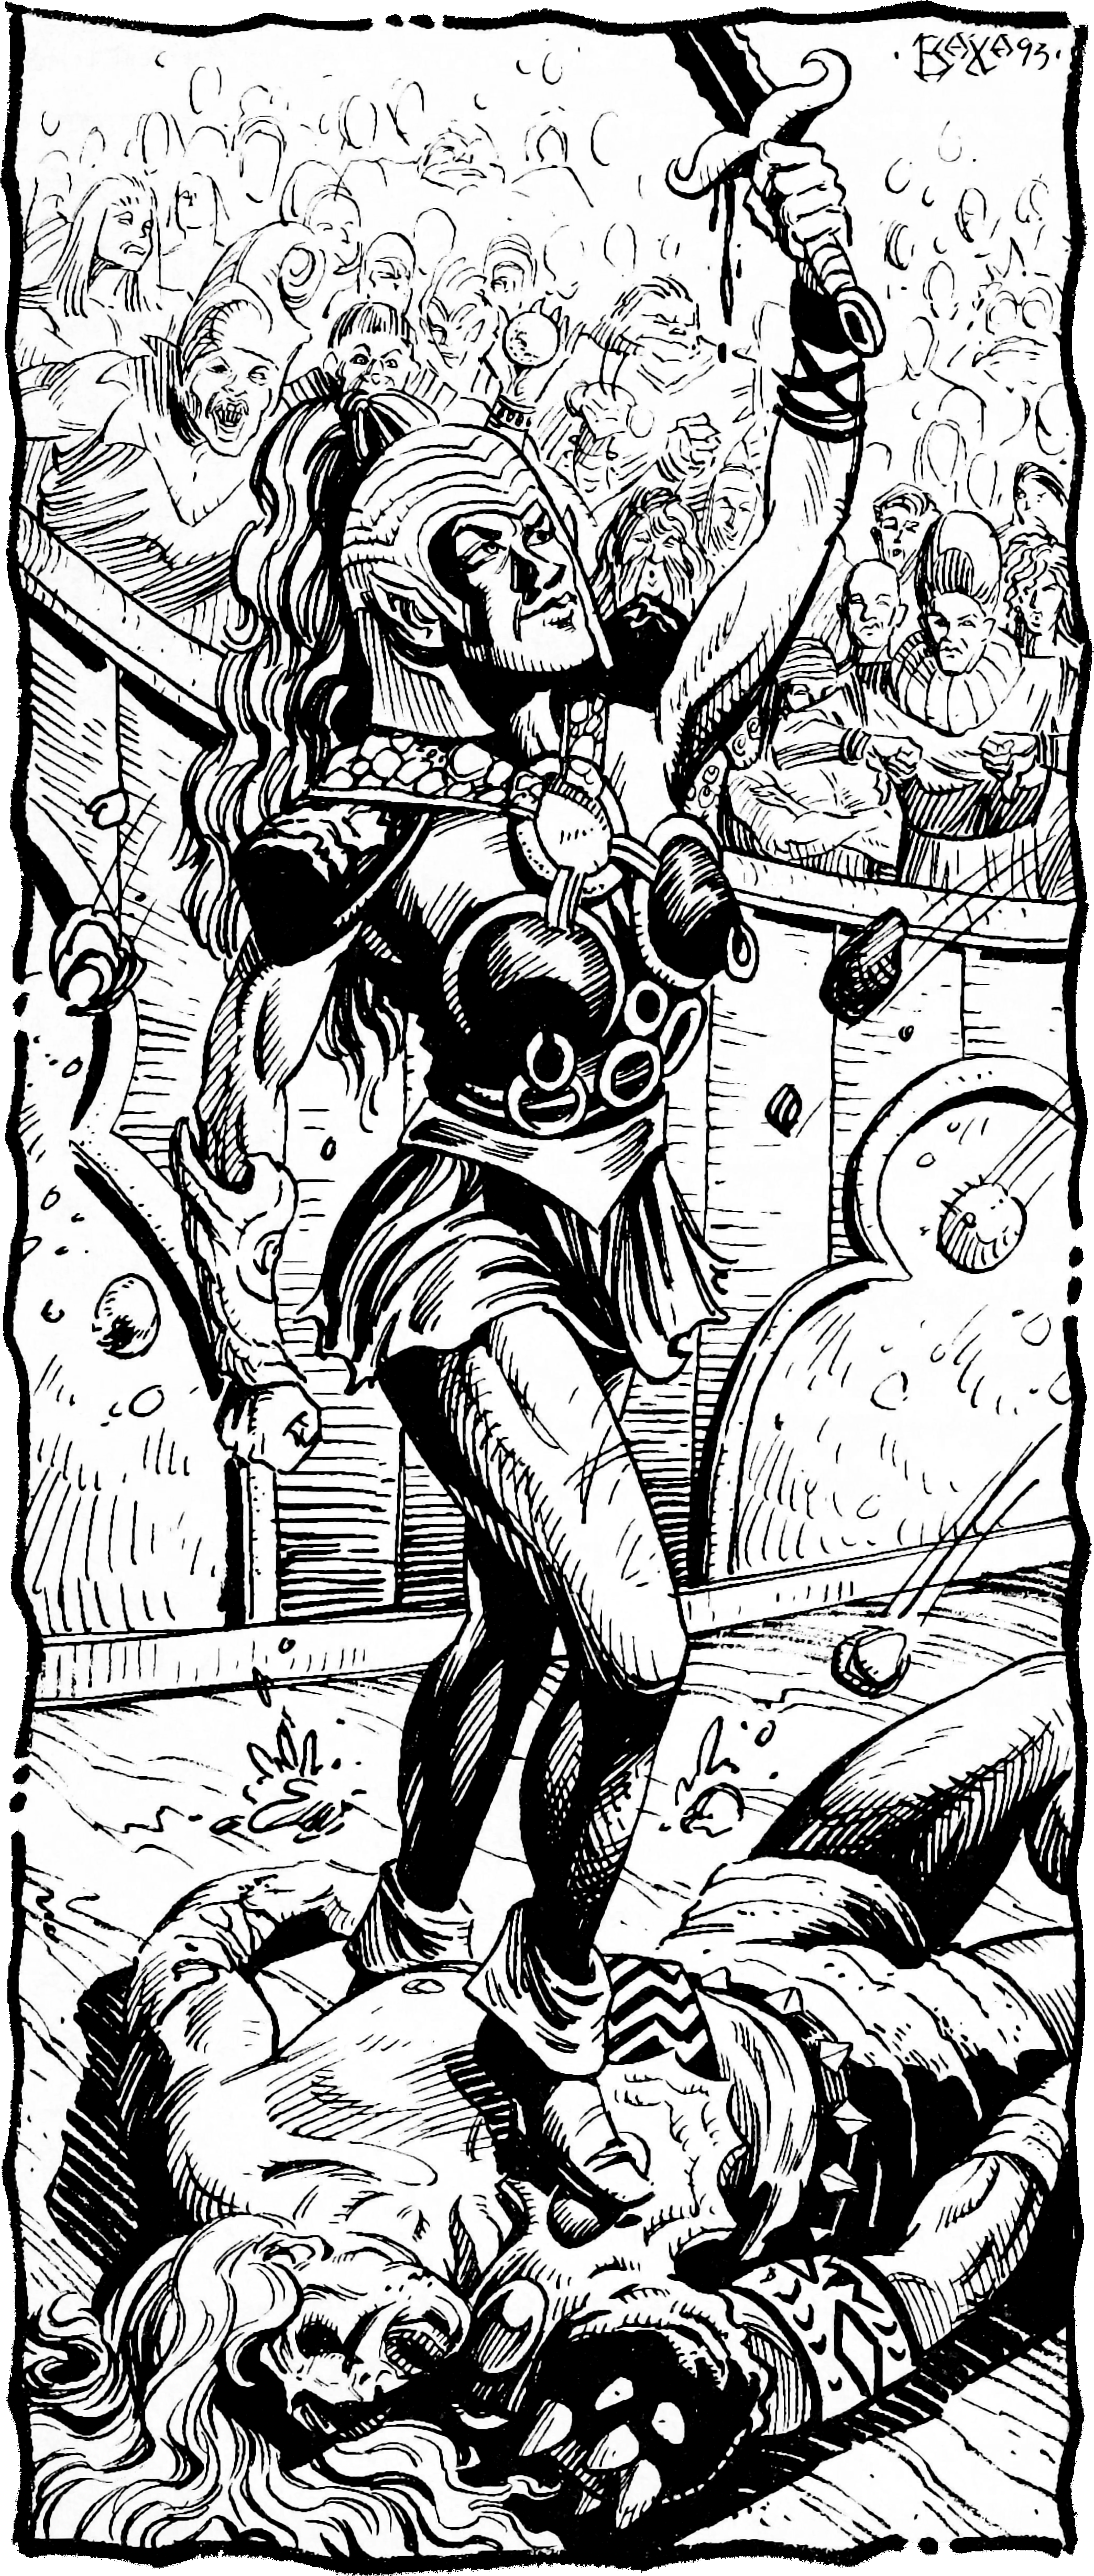
\includegraphics[width=\columnwidth]{images/gladiator-2.png}
\WOTC
\end{figure}

\subsection{Making a Gladiator}
Gladiators are among the best one-on-one fighters in all the Tablelands. They are trained in hand-to-hand combat before moving on to the use of exotic weapons of the arena. They learn to improvise weapons, wielding broken bones or wooden shafts with deadly precision. They learn how to taunt and tease opponents, driving them to reckless acts and taking advantage of the situation to strike down or maim a foe.

After all, a long, drawn-out combat is more a crowd pleaser than a ten-second bout.

\textbf{Abilities:} Strength and Constitution are vital to a gladiator, since he is often in harm's way. Intelligence is useful for gaining plenty of skills points, which a gladiator needs to purchase Bluff, Intimidate, Performance, and Sense Motive, key skills for any arena performer.

\textbf{Races:} All races of Athas can be found in the arenas of the Tablelands. Muls, with their mixed dwarven and human parentage, are highly prized in the arenas. They are often bought for a high price and treated well in return for victory on the combat floor. Elves are often used for their swiftness and natural flair for taunting their opponent. Humans are the most common of gladiators, since humans are the most common race in the Tablelands. Halflings make poor gladiators, since they abhor slavery and will usually starve themselves to death rather than being used as commodities by anyone. The savage races of the wastes are often used as gladiators, usually as fodder for the most successful gladiators, though those demonstrating excellent combat prowess receive formal training.

\textbf{Alignment:} Gladiators are of all alignments. Some gladiators will obey all arena rules, being lawful individuals, though these often do not last long in the arena. Many gladiators tend toward a chaotic alignment. Evil gladiators use dirty tricks to gain an advantage over an opponent. Gladiators of all alignments can become crowd favorites, increasing their chances of winning their matches, since often times these matches are prearranged. The intrigues of the city-states can reach deep into the arena.

\subsection{Game Rule Information}

\textbf{Hit Die:} d12.

\subsubsection{Class Skills}
\skill{Balance} (Dex), \skill{Bluff} (Cha), \skill{Climb} (Str), \skill{Craft} (Int), \skill{Intimidate} (Cha), \skill{Jump} (Str), \skill{Perform} (Cha), \skill{Profession} (Wis), \skill{Sense Motive} (Wis), \skill{Spot} (Wis), \skill{Tumble} (Dex).

\textbf{Skill Points per Level:} 4 + Int modifier ($\times4$ at 1st level).

\subsubsection{Class Features}

\textbf{Weapon and Armor Proficiency:} You are proficient with all simple and martial weapons, light armor, medium armor and shields (except tower shields).

\textbf{Gladiatorial Performance:} Once per day per gladiator level, you can use your talents to affect enemies and allies. Each ability requires both a minimum gladiator level and a minimum number of ranks in the \skill{Perform} skill to qualify.

Starting a gladiatorial performance effect is a standard action unless otherwise stated. Some effects require concentration, which means you must take a standard action each round to maintain the ability.

\textit{Combat Stance:} A gladiator with 3 or more ranks in \skill{Perform} can assume a combat stance, showing off to spectators and displaying a warning to opponents. You receive a +2 competence bonus to AC against the first attack made against you within 5 rounds after assuming the stance. Combat stance can be assumed as a move action. At 12th level, a gladiator can assume it as a swift action.

\textit{Martial Display:} A gladiator with 3 or more ranks in \skill{Perform} can entertain the crowd and intimidate enemies with a display of unarmed attacks or weapon prowess. You receive a +2 competence bonus to the first attack roll you make within 5 rounds after ending the martial display. Martial display can be assumed as a move action. At 12th level, a gladiator can use martial display as a swift action.

\textit{Team Strike:} A gladiator with 3 or more ranks in \skill{Perform} can distract an enemy so an ally can exploit a vital spot when making a melee attack. Team strike can only be used against an enemy you threaten with a melee weapon. The ally must act on the same initiative as you or before your next turn to gain the benefit of team strike. The ally receives a +1 bonus to hit and inflicts an additional 1d4 points of damage on the next melee attack against the target. If the enemy moves out of your threat range before your ally attacks, the ally does not receive the benefits of team strike. Creatures immune to sneak attack damage and critical hits are immune to team strike. At 7th level and every six levels thereafter these bonuses increase by +1 to attack and +1d4 to damage (+2 attack and +2d4 damage at 7th, +3 attack and +3d4 at 13th, +4 attack and +4d4 at 19th).

\textit{Taunt:} A gladiator of 3rd or higher level with 6 or more ranks in \skill{Perform} can demoralize enemies by verbal ridicule. Enemies must be within 9 meters of the gladiator and capable of hearing you, and you must be able to see your enemies. Each enemy affected suffers a $-1$ morale penalty to attack and damage rolls, and a $-1$ morale penalty on saving throws versus charm and fear effects. The effect lasts as long as enemies hear your taunts and for 5 rounds thereafter. At 8th level and every six gladiator levels thereafter, the penalties increase by 1 ($-2$ at 8th, $-3$ at 14th and $-4$ at 20th). Taunt is a mind-affecting ability.

\textit{Shake Off:} A gladiator of 6th or higher level with 9 or more ranks in \skill{Perform} can try to end a mind-affecting effect in play on himself or an ally. You shake your head violently to clear your mind, or slap an ally to bring her back to her senses. The recipient of the shake off can reroll a single failed save or opposed skill check (with the same DC as the failed roll) to end a mind-affecting effect. If there is no save or check to avoid the mind-affecting effect, the effect ends automatically.

\textit{Trick:} A gladiator of 9th or higher level with 12 or more ranks in \skill{Perform} can temporarily confuse an adversary through the use of ploy and deception. The creature to be tricked must be within 9 meters, able to see and hear you. You must also be able to see the creature. You make an opposed \skill{Bluff} check (vs. \skill{Sense Motive}) as a move action. If the creature succeeds on the opposed roll, you cannot attempt to trick that creature again for 24 hours. If its roll fails, the creature becomes dazed (unable to act, but can defend normally) for 1 round. For every three gladiator levels attained beyond 9th, you can target one additional creature with a single use of this ability (two at 12th level, three at 15th, four at 18th).

\textit{Chant:} A gladiator of 12th or higher level with 15 or more ranks in \skill{Perform} can start a chant. The chant boosts the gladiator or an ally's abilities, granting a +2 competence bonus to AC, skill checks and saving throws. To be affected an ally must be within 9 meters of you. For every three levels attained beyond 12th, you can affect one additional creature within 9 meters (two creatures at 15th level, three at 18th). Combat chant is a mind-affecting ability which lasts as long as you chant and for 5 rounds thereafter.

\textit{Threatening Glare:} A gladiator of 15th or higher with 18 or more ranks of \skill{Perform} can panic enemies with his mere gaze. Creatures within a 9 meters radius that can see you must make a Will Save (DC 10 + half your class level + your Charisma bonus). On failing, creatures with less HD than you are affected as if under the effects of a fear spell for 5 rounds. Those with equal to or more than your HD become shaken for 5 rounds. If the creature succeeds on the save you cannot attempt to affect that creature again for 24 hours. Threatening Glare is a mind-affecting gaze affect.

\textit{Dragon's Fury:} A gladiator of 18th or higher level with 21 or more ranks in \skill{Perform} can enter a trance-like state in which his full offensive gladiatorial potential is unleashed.

You are immune to fear effects, receive a +4 competence bonus to attack rolls and damage rolls, and an additional attack per round made at your highest base attack bonus. In addition, you gain two temporary hit points per class level. Dragon's fury lasts for 10 rounds.

\textbf{Mercy (Ex):} At 1st level, you suffer no penalty to attack rolls when attacking with a weapon to inflict nonlethal damage.

\textbf{Exotic Weapon:} At 1st, 5th, 9th, 13th, and 17th level, you receive \feat{Exotic Weapon Proficiency} as a bonus feat.

\textbf{Improved Unarmed Strike:} At 2nd level you \feat{Improved Unarmed Strike} as a bonus feat.

\textbf{Arena Guile (Ex):} Starting at 2nd level, you add one-half your gladiator level (round down) as a bonus to all \skill{Bluff} and \skill{Sense Motive} checks that relate directly to melee combat.

\textbf{Improved Feint:} You are adept at deceiving your opponents. At 3rd level, you gain \feat{Improved Feint} as a bonus feat.

\textbf{Uncanny Dodge (Ex):} At 4th level, you retain your Dexterity bonus to AC (if any) even if you are caught flat-footed or struck by an invisible attacker. However, you still lose your Dexterity bonus to AC if immobilized. If you already have uncanny dodge from a different class, you automatically gain improved uncanny dodge (see below) instead.

\textbf{Armor Optimization (Ex):} At 5th level, 10th, 15th, and 20th level, choose one of the following benefits which applies whenever you are wearing any armor you are proficient with:

\begin{itemize*}
\item +1 bonus to AC.
\item $-1$ armor check penalty.
\item +1 maximum Dexterity bonus.
\item Armor is treated as one category lighter (e.g. medium armor is treated as light armor).
\end{itemize*}

Each time this feature is gained, you must choose a different benefit.

\textbf{No Mercy (Ex):} Beginning at 6th level, you can perform a coup de grace as a standard action rather than a full-round action.

\textbf{Improved Uncanny Dodge (Ex):} At 8th level and higher, you can no longer be flanked. This defense denies a rogue the ability to sneak attack you by flanking you, unless the attacker has at least four more rogue levels than you have gladiator levels. If you already have uncanny dodge (see above) from a second class, the levels from all classes that grant uncanny dodge stack to determine the minimum level a rogue must be to flank you.

\textbf{Parry (Ex):} Beginning at 14th level, once per round you can forfeit an attack to attempt to parry an incoming melee attack. The forfeited attack has to be the one with your highest base attack bonus. If wielding two weapons, the parry must be made using your primary weapon. You make an opposed attack roll with a $-5$ penalty against your attacker roll. If you succeed, the attack is parried and you suffer no damage or ill effects related to the attack, including touch attacks used to deliver spells.

\textbf{Superior Feint:} Beginning at 15th level, you can make a \skill{Bluff} check to feint in combat as a free action, but only once per round.

\textbf{Improved Parry:} As parry (see above), except you no longer suffer a $-5$ penalty to your opposed attack roll.

\subsection{Playing a Gladiator}
Mastering the techniques of blade and shield is important to you, but even more is the sense of daring, danger, and even joy that you feel when you battle inside the arena. You fight for the glory, the thrill of combat, and for the adoration of the crowd. Thus, you approach each encounter as if the bards will sing of it for ages. Silver and concubines are pleasant tokens, but the real measure of your success is how loud the crowd screams your name when you step into the pit.

As a gladiator, you find adventure wherever an opportunity for glory exists. You might be one of the gladiators that went out of job when the sorcerer-king of you city was killed by Tyrians and now you have become a mercenary warrior, still looking for the thrill of combat. You might have been able to flee from your owner and now user your sword to protect your slave tribe.

\subsubsection{Religion}
Gladiators have no special religion of their own. Some may worship the sorcerer-king of the city-state they are in, while some few may worship the elemental forces. Often, the hard life of training and combat leaves the gladiator with little to think of except survival.

\subsubsection{Other Classes}
Gladiators tend to think of themselves as the superior warriors of the Tablelands, sometimes to the point of arrogance.

In a sense, though, they are right. Gladiators receive training in one-on-one combat, and the use of anything they can find as a weapon. However, a group of trained fighters fighting in concert is certainly a match for a bunch of gladiators, who are unused to fighting in groups. Like most people of Athas, gladiators have a deep distrust of magic, and tend to shun wizards. They view clerics as nothing more than healers, people who put their faith in abstract things rather than a sharp blade.

\subsubsection{Combat}
You revel in melee. Your place is battling against hulking baazrags and wicked tembo, where you can hear the crowd cheering and chanting your name. You make good use of your various trick abilities to give yourself an important edge in combat. Consider taking feats such as Toughness to increase your ability to soak up damage and partially offset your lack of heavy armor. Choose feats that enhance your combat capabilities (such as Arena Clamor and Brutal Attack) or increase your acting skills (such as Persuasive and Skill Focus).

Feints, tricks, and deception play a very important role in arena combat, but don't forget that you don't just need to win, you need to win dramatically. Pretend to be more wounded than you really are. Wait for the right to deliver the final blow.

\subsubsection{Advancement}
Gladiators come from all walks of like. Perhaps you were fascinated with the illustrious life the famous gladiators live. Perhaps you lost your freedom when your village was raided or because of debt, needing to fight for your freedom.

Your race matters little; anyone with the drive to win glory through arena combat is a good candidate for gladiator training. Although not everyone is as suited for arena combat as a mul or half-giant, but with enough training anyone can become a talented, or at least interesting gladiator.

As you become more skilled, your most important decisions are which specialization path you will take. The most common specialty paths are the blind-fighter, jazst, and the montare. The blind fighters specialize in a unique form of gladiatorial combat, battling in complete darkness. Jazst are widely traveled theatrical performers in the Athasian arenas and are usually early warm-up acts that amuse the eager crowds. Montare are gladiators who fight in mounted combat, riding a single mount, driving chariots or sometimes even a mobile war machine.

\subsection{Starting Packages}
\subsubsection{The Blind-Fighter}
Dwarf Gladiator

\textbf{Ability Scores:} Str 15, Dex 10, Con 15, Int 8, Wis 14, Cha 10.

\textbf{Skills:} \skill{Bluff}, \skill{Listen}, \skill{Perform}, \skill{Sense Motive}, \skill{Tumble}.

\textbf{Languages:} Common, Dwarven.

\textbf{Feat:} \feat{Blind-Fight}.

\textbf{Weapons:} Thanak (2d6/$\times$3).

\textbf{Armor:} Scale mail (+4 AC).

\textbf{Gear:} Standard adventurer's kit.

\subsubsection{The Jazst}
Elf Gladiator

\textbf{Ability Scores:} Str 10, Dex 17, Con 10, Int 8, Wis 13, Cha 14.

\textbf{Skills:} \skill{Bluff}, \skill{Diplomacy}, \skill{Intimidate}, \skill{Perform}, \skill{Sense Motive}, \skill{Tumble}.

\textbf{Languages:} Common, Elven.

\textbf{Feat:} \feat{Skill Focus} (Perform).

\textbf{Weapons:} Elven longblade (1d8/18--20).

\textbf{Armor:} Leather armor (+2 AC).

\textbf{Gear:} Standard adventurer's kit.

\vskip2cm
\subsubsection{The Montare}
Mul Gladiator

\textbf{Ability Scores:} Str 14, Dex 15, Con 13, Int 8, Wis 12, Cha 10.

\textbf{Skills:} \skill{Bluff}, \skill{Handle Animal}, \skill{Intimidate}, \skill{Perform}, \skill{Ride}, \skill{Sense Motive}.

\textbf{Languages:} Common.

\textbf{Feat:} \feat{Mounted Combat}.

\textbf{Weapons:} Heartpick (1d8/$\times$4)

Composite shortbow with 20 arrows (1d6/$\times$3, 21 m).

\textbf{Armor:} Leather armor (+2 AC).

\textbf{Gear:} Standard adventurer's kit.

\subsection{Gladiators on Athas}
\Quote{I am Darsus. I will be closer to you in these next few days, which will be the last days of your miserable lives, than the mother who first brought you screaming into this world. I did not pay good money for your company, I paid it so I could profit from your deaths. And just as your mother was there at your beginning, so I shall be there at your end. And when you die, and die you shall, your journey to the Gray will be to the sound of clapping and cheering. Don't let me down, and I won't feed your corpses to the jhakars.}{Darsus, arena manager}

In a world with civilizations as harsh as those of Athas, only the most bloodthirsty sports can entertain the crowds enough to keep their attention from their miserable lot in life. The arenas provide such sport with the spilling of blood by mighty gladiators. The killing is a release for the crowd, symbolic of that which the citizens cannot perform themselves.

It is therefore no wonder that the best of the gladiators rise above the crowd, to become the popular heroes of the age. Their exploits are the stuff of legends. Children follow their progress avidly, some even going so far as to paint the walls of the cities with pictures of their favorites in defiance of the templars. Some gladiators achieve such a measure of fame that their reputation spreads far from their city-states, bringing citizens of outlying towns to the arenas to witness these masters at their craft.

\subsubsection{Daily Life}

A gladiator must train constantly to maintain his puissance. Thus, much of his day is spent swinging wooden weapons, doing basic calisthenics, tightrope walking, and attending dodging practice. While out adventuring, a gladiator often spends time at night on watch practicing his move and stretching.

Once he has reached a respectable level of accomplishment, a gladiator might seek sponsorship from nobles and templars. These patrons offer better training and housing in return for no less than 50\% of the free gladiator's earnings and the companionship of the gladiator.

\subsubsection{Notables}

Famous gladiators usually fall into two categories: active gladiators who still perform in the many arenas of Athas, and former gladiators. Among those who still practice it there is Nightmare, a Gulgan blind gladiator who wears a great helm in the shape of a nightmare beast. Sandsinger is renowned elven jazst, and an accomplished dancer in and out of the arena. The most famous ex-gladiator of all is the mul Rikus of Tyr, responsible not for the death of one sorcerer-king, but three.

\subsubsection{Organizations}

High-level gladiators often find sponsorship from the rich. Nobles and templars will pay well to get an aspiring gladiator into their gladiator stables. Those cities that allow free gladiators to enter the games often have gladiators without such ties.

\subsubsection{NPC Reactions}

Easily motivated by promises of silver, glory, and freedom (whichever the employer possesses a surplus at the moment), gladiators can lend excellent, efficient muscle to any party. Most people look on gladiators with awe. The exception is when dealing with rival gladiators and their fans, which usually view them with contempt and try to belittle their abilities, generally displaying indifferent to unfriendly attitudes.

\subsubsection{Gladiator Lore}

Characters with ranks in \skill{Knowledge} (local) can research gladiators to learn more about them. When a character makes a skill check, read or paraphrase the following, including the information from lower DCs.

\textbf{DC 10:} A gladiator is a fighter with delusions of grandeur! These showoffs think they can live forever in a bard's song!

\textbf{DC 15:} Gladiators are extremely resilient and tricky combatants, and they seem to know with all kinds of weapons with the same degree of expertise.

\textbf{DC 20:} Some gladiators achieve such prestigious reputations that their fame spreads all over the Tablelands.

\Class{Psion}
{Resist all you like. I have ways of making you think.}{Dechares, Dwarven inquisitor}

The psion learns the Way, a philosophy of mental discipline, to become master of his will, or innate mental power. Most aspiring psions seek out an instructor, a master of the Way. Most Athasian cities contain psionic academies where students receive instructions in exchange for money or loyal service.

\PsychicTable{The Psion}{
1 & +0 & +0 & +0 & +2 & Bonus feat, discipline & 2 & 3 & 1st \\
2 & +1 & +0 & +0 & +3 &  & 6 & 5 & 1st \\
3 & +1 & +1 & +1 & +3 &  & 11 & 7 & 2nd \\
4 & +2 & +1 & +1 & +4 &  & 17 & 8 & 2nd \\
5 & +2 & +1 & +1 & +4 & Bonus feat & 25 & 11 & 3rd \\
6 & +3 & +2 & +2 & +5 &  & 35 & 13 & 3rd \\
7 & +3 & +2 & +2 & +5 &  & 46 & 15 & 4th \\
8 & +4 & +2 & +2 & +6 &  & 58 & 17 & 4th \\
9 & +4 & +3 & +3 & +6 &  & 72 & 19 & 5th \\
10 & +5 & +3 & +3 & +7 & Bonus feat & 88 & 21 & 5th \\
11 & +5 & +3 & +3 & +7 &  & 106 & 22 & 6th \\
12 & +6/+1 & +4 & +4 & +8 &  & 126 & 24 & 6th \\
13 & +6/+1 & +4 & +4 & +8 &  & 147 & 25 & 7th \\
14 & +7/+2 & +4 & +4 & +9 &  & 170 & 27 & 7th \\
15 & +7/+2 & +5 & +5 & +9 & Bonus feat & 195 & 28 & 8th \\
16 & +8/+3 & +5 & +5 & +10 &  & 221 & 30 & 8th \\
17 & +8/+3 & +5 & +5 & +10 &  & 250 & 31 & 9th \\
18 & +9/+4 & +6 & +6 & +11 &  & 280 & 33 & 9th \\
19 & +9/+4 & +6 & +6 & +11 &  & 311 & 34 & 9th \\
20 & +10/+5 & +6 & +6 & +12 & Bonus feat & 343 & 36 & 9th}

\begin{figure}[t!]
\centering
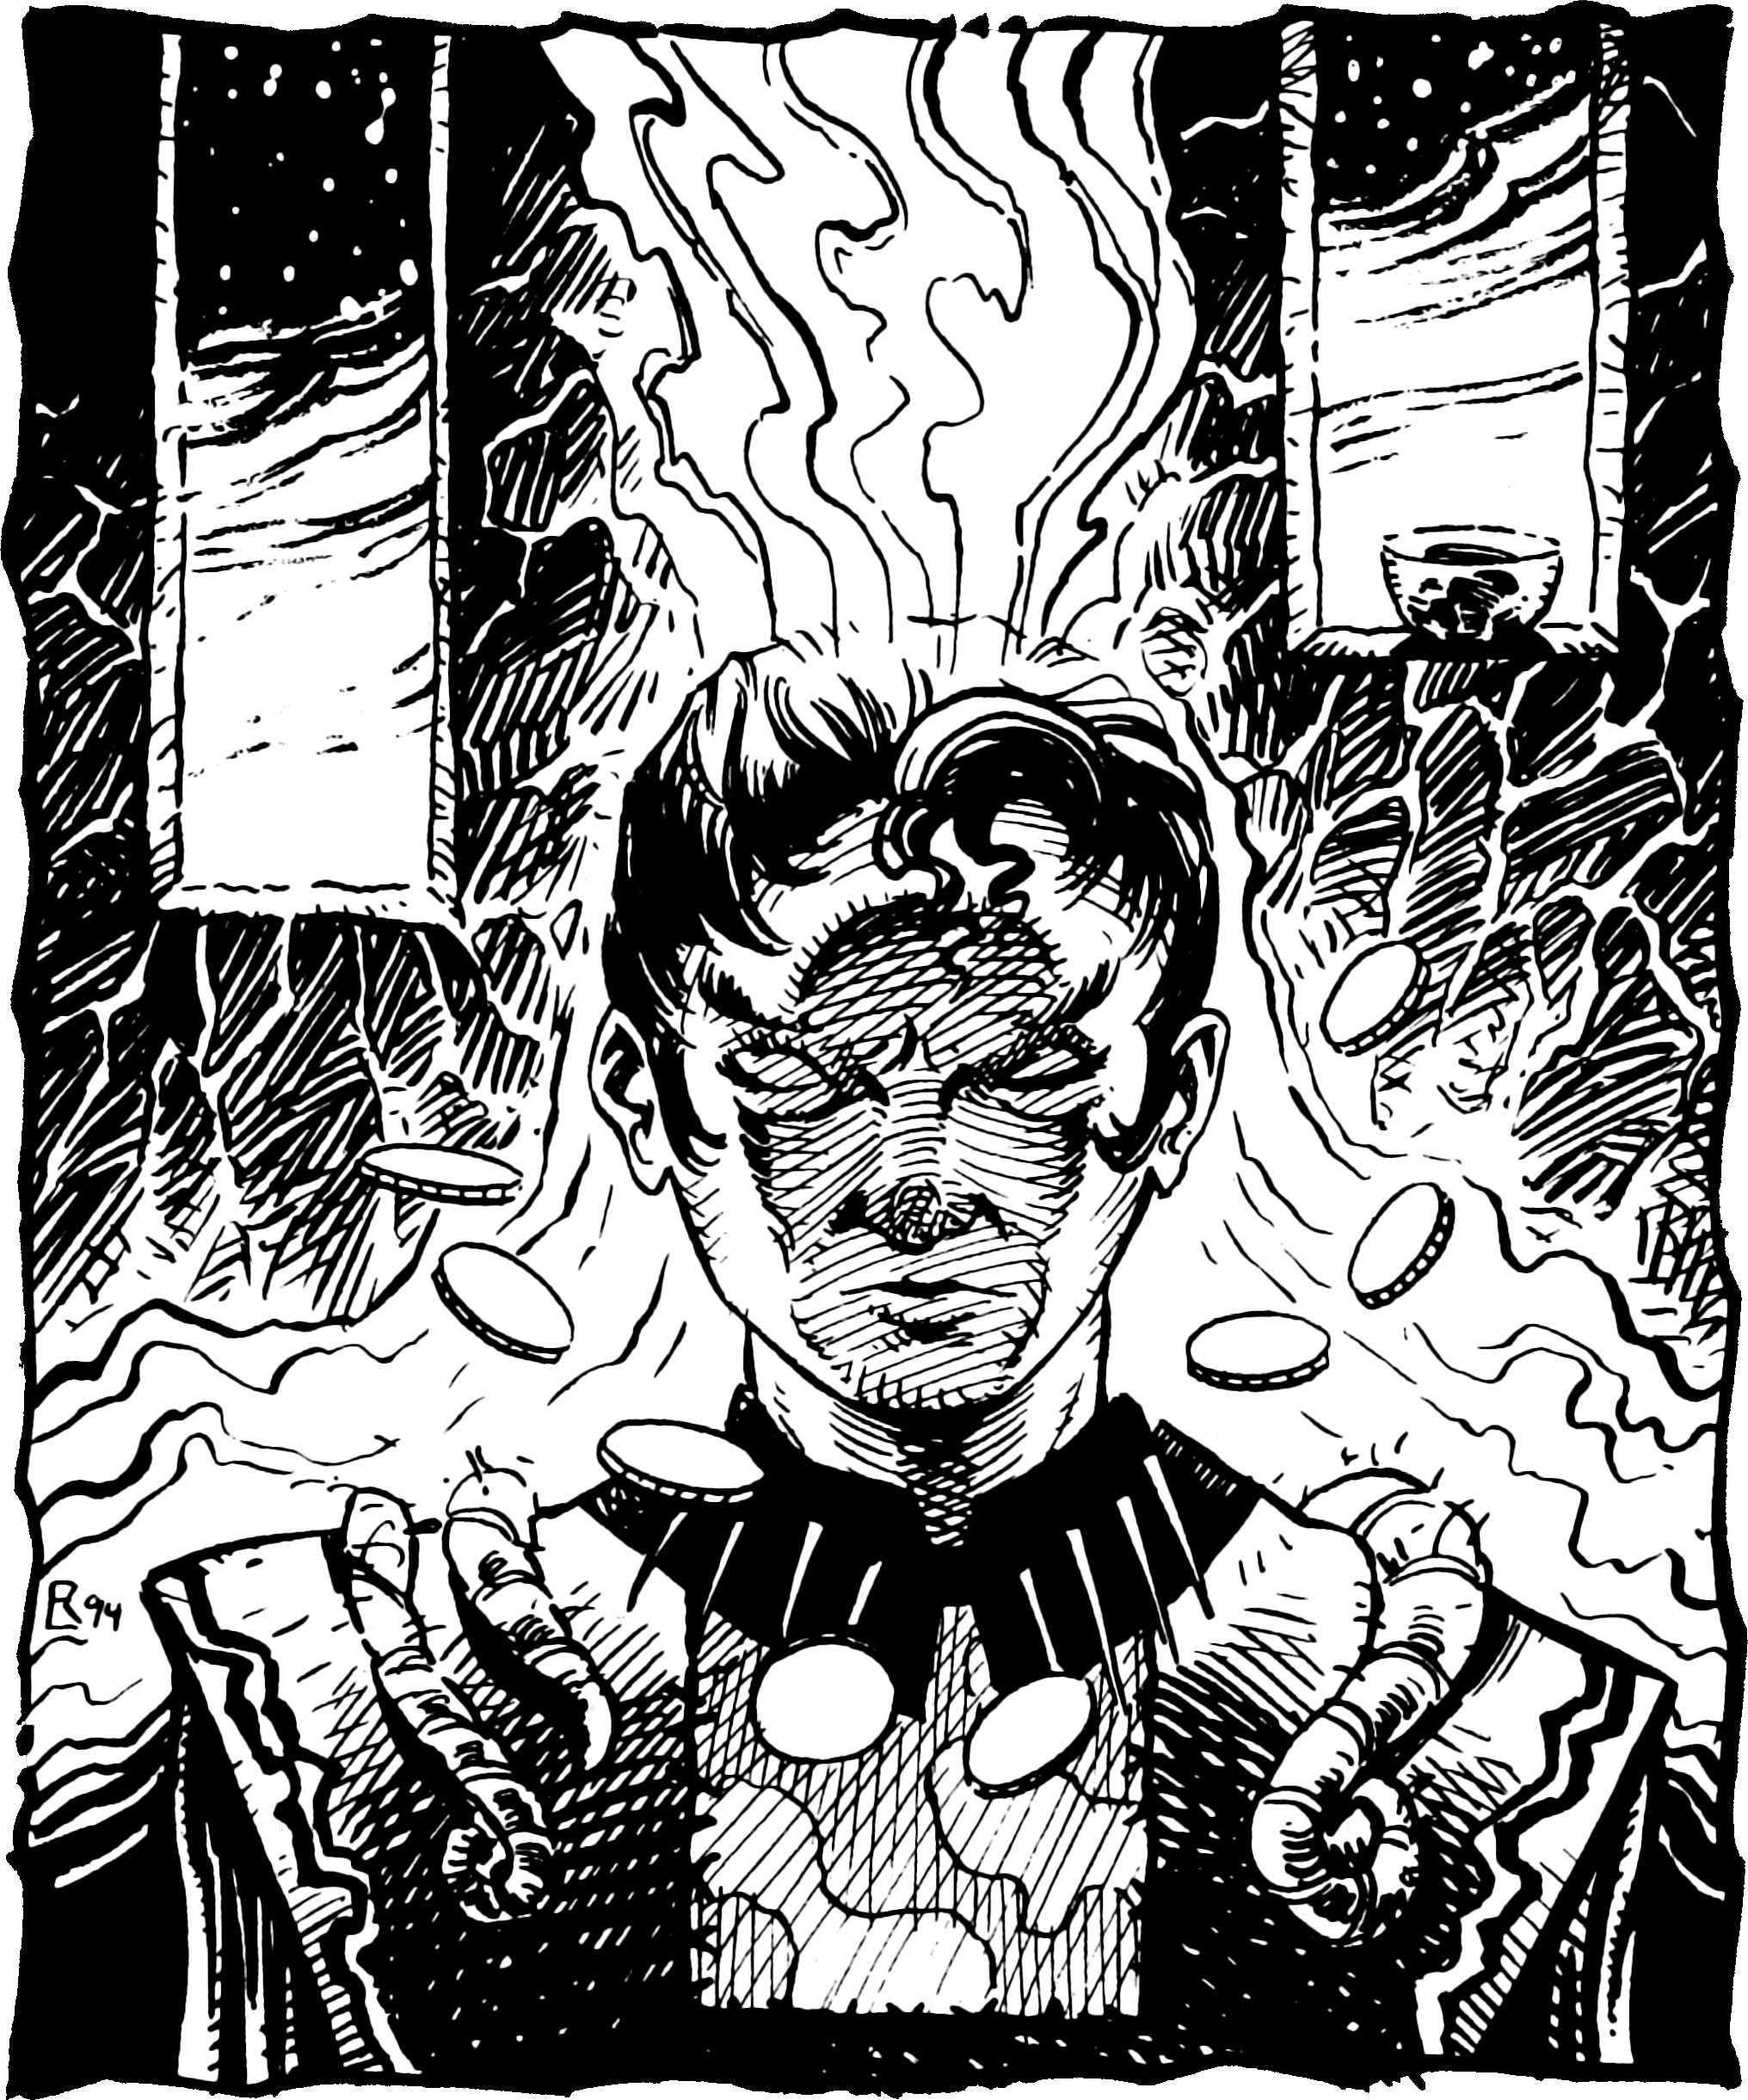
\includegraphics[width=\columnwidth]{images/psion-2.png}
\WOTC
\end{figure}

\subsection{Making a Psion}
The psion learns the Way in order to shape his Will. The psion uses, through study called the Way, how to manifest the power inherent in his inner self. The psion is able to project this power, the Will, into creating all sorts of supernatural effects. The psion may know a limited number of ways to shape his will, but he enjoys great flexibility in how he uses his known powers.

\textbf{Races:} Nearly all living creatures have a latent psionic capacity, and psions are found among all sentient races of the Tablelands, and even among some creatures that are not ordinarily considered sentient.

\textbf{Alignment:} The search for refinement of the Way tends to draw many psions into a neutral view of the world, so most psions have one part of their alignment that is neutral. Good psions may spend their time in search of new powers, or help their village defend itself against predators, or maybe join the ranks of Merchant Houses. Evil psions may serve as agents in service of the sorcerer-kings, or as more shady agents of Merchant Houses, or simply work as mercenaries and offer their specialized services to the highest bidder. Even though many psions tend to have a neutral view of the world, they can be of any alignment.

\subsection{Game Rule Information}

\textbf{Hit Die:} d4.

\subsubsection{Class Skills}

\skill{Concentration} (Con), \skill{Craft} (Int), \skill{Knowledge} (all skills, taken individually) (Int), \skill{Profession} (Wis), and \skill{Psicraft} (Int). In addition, a psion gains access to additional class skills based on his discipline:

\textbf{Seer (Clairsentience):} \skill{Gather Information} (Cha), \skill{Listen} (Wis), and \skill{Spot} (Wis).

\textbf{Shaper (Metacreativity):} \skill{Bluff} (Cha), \skill{Disguise} (Cha), and \skill{Use Psionic Device} (Cha).

\textbf{Kineticist (Psychokinesis):} \skill{Autohypnosis} (Wis), \skill{Disable Device} (Dex), and \skill{Intimidate} (Cha).

\textbf{Egoist (Psychometabolism):} \skill{Autohypnosis} (Wis), \skill{Balance} (Dex) and \skill{Heal} (Wis).

\textbf{Nomad (Psychoportation):} \skill{Climb} (Str), \skill{Jump} (Str), \skill{Ride} (Dex), \skill{Survival} (Wis), and \skill{Swim} (Str).

\textbf{Telepath (Telepathy):} \skill{Bluff} (Cha), \skill{Diplomacy} (Cha), \skill{Gather Information} (Cha), and \skill{Sense Motive} (Wis).

\textbf{Skill Points per Level:} 2 + Int modifier ($\times 4$ at 1st level).

\subsubsection{Class Features}

\textbf{Weapon and Armor Proficiency:} Psions are proficient with the club, dagger, heavy crossbow, light crossbow, quarterstaff, and shortspear. They are not proficient with any type of armor or shield. Armor does not, however, interfere with the manifestation of powers.

\textbf{Power Points per Day:} A psion's ability to manifest powers is limited by the power points he has available. His base daily allotment of power points is given on \tabref{The Psion}. In addition, he receives bonus power points per day if he has a high Intelligence score (see \tabref{Ability Scores and Bonus Power Points}). His race may also provide bonus power points per  day, as may certain feats and items.

\textbf{Discipline:} Every psion must decide at 1st level which psionic discipline he will specialize in. Choosing a discipline provides a psion with access to the class skills associated with that discipline (see above), as well as the powers restricted to that discipline. However, choosing a discipline also means that the psion cannot learn powers that are restricted to other disciplines. He can't even use such powers by employing psionic items.

\textbf{Powers Known:} A psion begins play knowing three psion powers of your choice. Each time he achieves a new level, he unlocks the knowledge of new powers.

Choose the powers known from the psion power list, or from the list of powers of your chosen discipline. You cannot choose powers from restricted discipline lists other than your own discipline list. You can choose powers from disciplines other than your own if they are not on a restricted discipline list. (Exception: The feats Expanded Knowledge and Epic Expanded Knowledge do allow a psion to learn powers from the lists of other disciplines or even other classes.) A psion can manifest any power that has a power point cost equal to or lower than his manifester level.

The number of times a psion can manifest powers in a day is limited only by his daily power points.

A psion simply knows his powers; they are ingrained in his mind. He does not need to prepare them (in the way that some spellcasters prepare their spells), though he must get a good night's sleep each day to regain all his spent power points.

The Difficulty Class for saving throws against psion powers is 10 + the power's level + the psion's Intelligence modifier. Maximum Power Level Known: A psion begins play with the ability to learn 1st-level powers. As he attains higher levels, a psion may gain the ability to master more complex powers.

To learn or manifest a power, a psion must have an Intelligence score of at least 10 + the power's level.

\textbf{Bonus Feats:} A psion gains a bonus feat at 1st level, 5th level, 10th level, 15th level, and 20th level. This feat must be a psionic feat, a metapsionic feat, or a psionic item creation feat.

These bonus feats are in addition to the feats that a character of any class gains every three levels. A psion is not limited to psionic feats, metapsionic feats, and psionic item creation feats when choosing these other feats.

\subsubsection{Psionic Disciplines}
A discipline is one of six groupings of powers, each defined by a common theme. The six disciplines are clairsentience, metacreativity, psychokinesis, psychometabolism, psychoportation, and telepathy.

\textbf{Clairsentience:} A psion who chooses clairsentience is known as a seer. Seers can learn precognitive powers to aid their comrades in combat, as well as powers that permit them to gather information in many different ways.

\textbf{Metacreativity:} A psion specializing in metacreativity is known as a shaper. This discipline includes powers that draw ectoplasm or matter from the Astral Plane, creating semisolid and solid items such as armor, weapons, or animated constructs to do battle at the shaper's command.

\textbf{Psychokinesis:} Psions who specialize in psychokinesis are known as kineticists. They are the masters of powers that manipulate and transform matter and energy. Kineticists can attack with devastating blasts of energy.

\textbf{Psychometabolism:} A psion who specializes in psychometabolism is known as an egoist. This discipline consists of powers that alter the psion's psychobiology, or that of creatures near him. An egoist can both heal and transform himself into a fearsome fighter.

\textbf{Psychoportation:} A psion who relies on psychoportation powers is known as a nomad. Nomads can wield powers that propel or displace objects in space or time.

\textbf{Telepathy:} A psion who chooses the discipline of telepathy is known as a telepath. He is the master of powers that allow mental contact and control of other sentient creatures. A telepath can deceive or destroy the minds of his enemies with ease.

\subsubsection{Psicrystals}

\begin{figure}[t!]
\centering
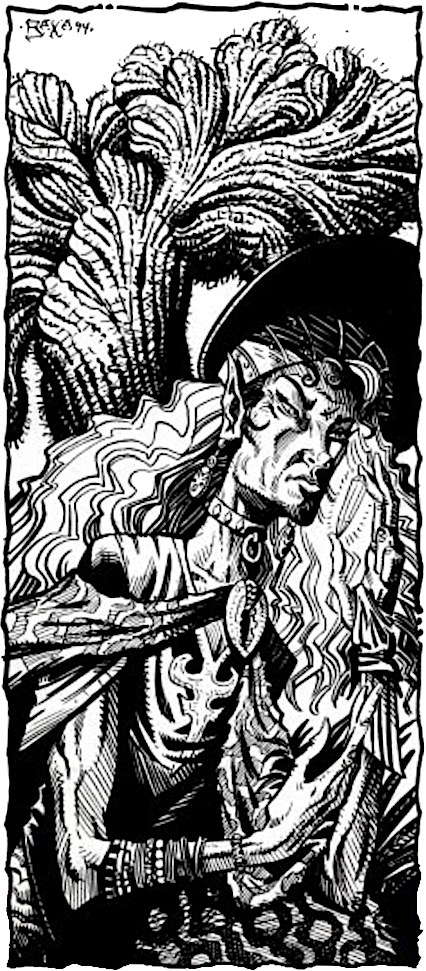
\includegraphics[width=\columnwidth-2mm]{images/psion-3.png}
\WOTC
\end{figure}

A psicrystal is a fragment of a psionic character's personality, brought into physical form and a semblance of life (via the \feat{Psicrystal Affinity} feat). A psicrystal appears as a crystalline construct about the size of a human hand.

Because it is an extension of its creator's personality, a character's psicrystal is in some ways a part of him. That's why, for example, a psionic character can manifest a personal range power on his psicrystal even though normally he can manifest such a power only on himself.

A psicrystal is treated as a construct for the purposes of all effects that depend on its type.

A psicrystal grants special abilities to its owner, as shown on the \tabref{Psicrystal Special Abilities}. In addition, a psicrystal has a personality (being a fragment of the owner's personality), which gives its owner a bonus on certain types of checks or saving throws, as given on the Psicrystal Personalities table below. These special abilities and bonuses apply only when the owner and the psicrystal are within 1.5 kilometer of each other.

Psicrystal abilities are based on the owner's levels in psionic classes. Levels from other classes do not count toward the owner's level for purposes of psicrystal abilities.

A psicrystal can speak one language of its owner's choice (so long as it is a language the owner knows). A psicrystal can understand all other languages known by its owner, but cannot speak them. This is a supernatural ability.

\textbf{Psicrystal Basics:} Use the statistics for a psicrystal, but make the following changes.

\textit{Saving Throws:} A psicrystal uses its owner's base saving throw bonuses and ability modifiers on saves, though it doesn't enjoy any other bonuses its owner might have (from magic items or feats, for example).

\textit{Abilities:} When its self-propulsion ability is not activated, a psicrystal has no Strength score and no Dexterity score.

\textit{Skills:} A psicrystal has the same skill ranks as its owner, except that it has a minimum of 4 ranks each in \skill{Spot}, \skill{Listen}, \skill{Move Silently}, and \skill{Search}. (Even if its owner has no ranks in these skills, a psicrystal has 4 ranks in each.) A psicrystal uses its own ability modifiers on skill checks.

\Table{Psicrystal Special Abilities}{X C Z{1cm} b{4.2cm}} {
\tableheader Owner Level & \tableheader Natural Armor Adj. & \tableheader Int Adj. & \tableheader Special \\
1--2 & +0 & +0 & Alertness, improved evasion, personality, self-propulsion, share powers, sighted, telepathic link \\
3--4 & +1 & +1 & Deliver touch powers \\
5--6 & +2 & +2 & Telepathic speech \\
7--8 & +3 & +3 &\\
9--10 & +4 & +4 & Flight \\
11--12 & +5 & +5 & Power resistance \\
13--14 & +6 & +6 & Sight link \\
15--16 & +7 & +7 & Channel power \\
17--18 & +8 & +8 &\\
19--20 & +9 & +9 &
}

\textbf{Psicrystal Ability Descriptions:} All psicrystals have special abilities (or impart abilities to their owners) depending on the level of the owner, as shown on the table above. The abilities on the table are cumulative.

\textit{Natural Armor Adj. (Ex):} This number noted here is an improvement to the psicrystal's natural armor bonus (normally 0). It represents a psicrystal's preternatural durability.

\textit{Intelligence Adj. (Ex):} Add this value to the psicrystal's Intelligence score. Psicrystals are as smart as people (though not necessarily as smart as smart people).

\textit{Alertness (Ex):} The presence of a psicrystal sharpens its master's senses. While a psicrystal is within arm's reach (adjacent to or in the same square as its owner), its owner gains the Alertness feat.

\textit{Improved Evasion (Ex):} If a psicrystal is subjected to an attack that normally allows a Reflex saving throw for half damage, it takes no damage if it makes a successful saving throw and half damage even if the saving throw fails.

\textit{Personality (Ex):} Every psicrystal has a personality. See Psicrystal Personality, below.

\textit{Self-Propulsion (Su):} As a standard action, its owner can will a psicrystal to form spidery, ectoplasmic legs that grant the psicrystal a land speed of 9 meters and a climb speed of 6 meters. The legs fade into nothingness after one day (or sooner, if the owner desires).

\textit{Share Powers (Su):} At the owner's option, he can have any power (but not any psi-like ability) he manifests on himself also affect his psicrystal. The psicrystal must be within 1.5 meter of him at the time of the manifestation to receive the benefit. If the power has a duration other than instantaneous, it stops affecting the psicrystal if it moves farther than 1.5 meter away, and will not affect the psicrystal again, even if it returns to its owner before the duration expires.

Additionally, the owner can manifest a power with a target of ``You'' on his psicrystal (as a touch range power) instead of on himself. The owner and psicrystal cannot share powers if the powers normally do not affect creatures of the psicrystal's type (construct).

\textit{Sighted (Ex):} Although it has no physical sensory organs, a psicrystal can telepathically sense its environment as well as a creature with normal vision and hearing. Darkness (even supernatural darkness) is irrelevant, as are areas of supernatural silence, though a psicrystal still can't discern invisible or ethereal beings. A psicrystal's sighted range is 12 meters.

\textit{Telepathic Link (Su):} The owner has a telepathic link with his psicrystal out to a distance of up to 1.5 kilometer. The owner cannot see through the psicrystal's senses, but the two of them can communicate telepathically as if the psicrystal were the target of a mindlink power manifested by the owner. For instance, a psicrystal placed in a distant room could relay the activities occurring in that room.

Because of the telepathic link between a psicrystal and its owner, the owner has the same connection to an item or place that the psicrystal does. For instance, if his psicrystal has seen a room, the owner can teleport into that room as if he has seen it too.

\textit{Deliver Touch Powers (Su):} If the owner is 3rd level or higher, his psicrystal can deliver touch powers for him. If the owner and psicrystal are in contact at the time the owner manifests a touch power, he can designate his psicrystal as the ``toucher.'' The psicrystal can then deliver the touch power just as the owner could. As usual, if the owner manifests another power before the touch is delivered, the touch power dissipates.

\textit{Telepathic Speech (Ex):} If the owner is 5th level or higher, the psicrystal can communicate telepathically with any creature that has a language and is within 9 meters of the psicrystal, while the psicrystal is also within 1.5 kilometer of the owner.

\textit{Flight (Su):} If the owner is 9th level or higher, he can, as a standard action, will his psicrystal to fly at a speed of 15 meters (poor). The psicrystal drifts gently to the ground after one day (or sooner, if the owner desires).

\textit{Power Resistance (Ex):} If the owner is 11th level or higher, the psicrystal gains power resistance equal to the owner's level + 5. To affect the psicrystal with a power, another manifester must get a result on a manifester level check that equals or exceeds the psicrystal's power resistance.

\textit{Sight Link (Sp):} If the owner is 13th level or higher, the character can remote view the psicrystal (as if manifesting the remote view power) once per day.

\textit{Channel Power (Sp):} If the owner is 15th level or higher, he can manifest powers through the psicrystal to a distance of up to 1.5 kilometer. The psicrystal is treated as the power's originator, and all ranges are calculated from its location.

When channeling a power through his psicrystal, the owner manifests the power by paying its power point cost. He is still subject to attacks of opportunity and other hazards of manifesting a power, if applicable (for instance, he becomes visible when manifesting an offensive power if invisible, as does the psicrystal).

\Table{Psicrystal Personalities}{b{2cm} X}{
\tableheader Personality & \tableheader Benefit to Owner\\
Artiste & +3 bonus on \skill{Craft} checks\\
Bully & +3 bonus on \skill{Intimidate} checks\\
Coward & +3 bonus on \skill{Hide} checks\\
Friendly & +3 bonus on \skill{Diplomacy} checks\\
Hero & +2 bonus on Fortitude saves\\
Liar & +3 bonus on \skill{Bluff} checks\\
Meticulous & +3 bonus on \skill{Search} checks\\
Nimble & +2 bonus on Initiative checks\\
Observant & +3 bonus on \skill{Spot} checks\\
Poised & +3 bonus on \skill{Balance} checks\\
Resolved & +2 bonus on Will saves\\
Sage & +3 bonus on checks involving any one \skill{Knowledge} skill owner already knows; once chosen, this does not vary\\
Single-minded & +3 bonus on \skill{Concentration} checks\\
Sneaky & +3 bonus on \skill{Move Silently} checks\\
Sympathetic & +3 bonus on \skill{Sense Motive} checks
}

\textbf{Psicrystal Personality (Ex):} Each psicrystal has a distinct personality, chosen by its owner at the time of its creation from among those given on the following table. At 1st level, its owner typically gets a feel for a psicrystal's personality only through occasional impulses, but as the owner increases in level the psicrystal's personality becomes more pronounced. At higher levels, it is not uncommon for a psicrystal to constantly ply its owner with observations and advice, often severely slanted toward the psicrystal's particular worldview. The owner always sees a bit of himself in his psicrystal, even if magnified and therefore distorted.

\subsection{Playing a Psion}
When you first learned to use psionics, you were taught to create a nexus---a point in the center of your being where physical, mental, and spiritual energy can be harnessed. It is the union of these powers that allows you to perform the remarkable feats you're capable of.

As a psion, your choice of discipline is all-important to you. Seers are not very powerful, if one defines power as the ability to cause immediate harm to one's foes, but they are the most capable information gatherers of Athas. Shapers are tinkerers, creating toys and monsters out of thin air, just to dismiss them and build another. Kineticists are battlefield psionicists who are actively sought out as military auxiliaries, and is almost as good as a wizard for creating mayhem in a fight. Egoists have a wide range of useful powers: they can fight as well as a fighter, become stealthier than a thief, heal like a cleric, or change shape like a wizard. Nomads possess an array of valuable powers that can bypass almost any obstacle and confound any enemies, working with the very fabric of space, time, and reality itself to achieve his goals. Telepaths are considered by some to the most powerful psions, and most Athasians are terrified of a telepath's ability to manipulate their very thoughts.

\subsubsection{Religion}
Psions use the Way to manifest their inner powers; through long hours of meditation and extremes of the senses, they seek knowledge inward. Their power comes from inside them, so only psions from the most animistic cultures look to outside beings or religions for spiritual fulfillment.

\subsubsection{Other Classes}
Psions tend to be drawn to those like themselves. Lower-level psions tend to towards a nearly worshipful attitude towards higher level psions, curious about their mysterious training and knowledge.

Higher-level psions tend to either stay to themselves, or to try to befriend almost everyone, pressing for party leadership. Most psions tolerate priests and druids (although some psions make needling remarks about ``foolish superstition''), but most psions are uneasy with wizards. Psions view wilders much in the same way that a fighter views a barbarian---untrained, erratic, and as much a danger to his companions as to his enemies.

\subsubsection{Combat}

You usually disdain combat and other primitive displays of force, but when needed, you use your impressive array of psionic powers for both attack and defense against your enemies, just as any other psionic character would.

\subsubsection{Advancement}

Most psions were strongly inclined towards a specific discipline before their ever realized they had any psionic talent. Once you have undergone your initial training, you can continue your studies on your own, much the way a wizard learn new spells.

As you attain more levels in the psion class, the most important choice you face is which powers to learn. A psion has access to much fewer spells than a wizard, so he has to chose carefully in order to find a good mix of offensive, defensive, and utility powers.

\subsection{Starting Packages}
\subsubsection{The Blaster}

Aarakocra Psion (Kineticist)

\textbf{Ability Scores:} Str 8, Dex 18, Con 13, Int 15, Wis 12, Cha 6.

\textbf{Skills:} \skill{Concentration}, \skill{Intimidate}, \skill{Knowledge} (psionics), \skill{Psicraft}.

\textbf{Languages:} Auran, Common.

\textbf{Feat:} \feat{Overchannel}.

\textbf{Weapons:} Shortspear (1d6, 6 m)

Light crossbow with 20 bolts (1d6/19--20, 24 m).

\textbf{Armor:} None.

\textbf{Other Gear:} Standard adventurer's kit, 62 cp.

\subsubsection{The Mindbender}
Human Psion (Telepath)

\textbf{Ability Scores:} Str 8, Dex 10, Con 12, Int 15, Wis 13, Cha 14.

\textbf{Skills:} \skill{Bluff}, \skill{Concentration}, \skill{Gather Information}, \skill{Knowledge} (local), \skill{Sense Motive}.

\textbf{Languages:} Common.

\textbf{Feat:} \skill{Inquisitor}, \skill{Psionic Endowment}.

\textbf{Weapons:} Club (1d4)

Light crossbow with 20 bolts (1d6/19--20, 24 m).

\textbf{Armor:} None.

\textbf{Other Gear:} Standard adventurer's kit, 63 cp.

\subsubsection{The Teleporter}
Elf Psion (Nomad)

\textbf{Ability Scores:} Str 10, Dex 16, Con 10, Int 15, Wis 13, Cha 8.

\textbf{Skills:} \skill{Concentration}, \skill{Jump}, \skill{Psicraft}, \skill{Survival}.

\textbf{Languages:} Elven, Common.

\textbf{Feat:} \feat{Speed of Thought}.

\textbf{Weapons:} Quarterstaff (1d6)

Dagger (1d4/19--20, 3 m)

Shortbow with 20 arrows (1d6/$\times$3. 18 m).

\textbf{Armor:} None.

\textbf{Other Gear:} Standard adventurer's kit, 64 cp.

% \vskip5cm
\subsection{Psions on Athas}
\Quote{Once, I encountered a shattered tribe of elves wandering aimlessly through the desert. Lost and unprovisioned, they clearly had no hope of survival beyond the next few days. I later learned that they had made the mistake of disturbing a psionic master's trance as they attempted to rob his home.}{The Wanderer's Journal}

Nearly every level of Athasian society is permeated with psionics. Even the humblest slave may possess an unusual talent or ability, while the most powerful enchantments of the sorcerer-monarchs include psionic elements. Mental powers are used on an everyday basis in Athasian culture.

Telepaths allow instantaneous communication across hundreds of miles. Draft animals and slaves are kept under control by psionic overseers. Prophets use their visionary powers to forecast the fortunes of kings and peasants, find missing objects, and solve crimes. Kineticists and egoists use their potent abilities in all manner of enterprises, both legitimate and otherwise.

\subsubsection{Daily Life}

The study of the Way is very similar to the study of magic. Just as wizards strive to master more advanced and difficult spells, psionicists must constantly seek to unlock new and more powerful abilities. Unlike wizardry, there is no single formula that will reproduce an effect of the Way that will work the same for each individual. Students must independently develop the command of their powers.

High-level psions tend to become contemplative masters, so they can make good patrons for lower-level PCs. Such psions often hire adventurers to gather rare psionic items for study or to recover lost knowledge of the ancient ages in their stead.

\subsubsection{Notables}

The human psion known as Pharistes brought chaos over the Tyr Region when he activated a powerful artifact that dampened all psionic power in the region and drove all thri-kreen mad because he thought the abuse of psionics was the cause of all the evil under the dark sun. Agis of Asticles was an accomplished telepath and politician, who fought to bring freedom to the city-stated of Tyr and helped to remove Athas from the menace of the Dragon of Tyr.

\subsubsection{Organizations}

Psions don't organize together, but they often join other organizations, specially psionic academies and monasteries. Psions who dedicate themselves into extensive studies in such organizations in order to master the Way often become \class{Psiologists}.

\subsubsection{NPC Reactions}

The common people usually react to a psion exactly as they would to any other psionicists in their community. Because trained psionicists are scarce and their skills are vital, they are highly valued by many elements of the Athasian society. Unlike wizards, psionicists are free of the taint of magic and need not disguise their calling. They owe no loyalty to the sorcerer-kings, unlike the templars. Even clerics and druids have elemental powers and guarded lands that they must place before all other considerations. Psionicists are free of these patrons and responsibilities and may employ their powers as they see fit.

\subsubsection{Psion Lore}

Characters with ranks in \skill{Knowledge} (psionics) can research psions to learn more about them. When a character makes a skill check, read or paraphrase the following, including the information from lower DCs.

\textbf{DC 10:} Psions are manifesters who use the forces of their own minds to affect their environment.

\textbf{DC 15:} Psionic powers do not draw upon magical energy that surrounds all things. Rather they are derived from within when the psionicist has his entire essence in coordination; his mind, body, and soul in perfect harmony.

\textbf{DC 20:} Psions choose one of the six psionic disciplines in which to focus their efforts.

\Class{Psychic Warrior}
{The body is not bound to the forms and function you were born with. To master the art of delivering death, you must break your given mold.}{Tharlkar, psychic sense}

The term ``psychic warrior'' is a loose translation of the Thri-kreen word ``chakak,'' which is better translated as ``mind warrior.'' In the Tablelands, non-kreen psychic warriors have long been known as ``mercenary psionicists.''

\PsychicTable{The Psychic Warrior}{
1 & +0 & +2 & +0 & +0 & Bonus feat & 0 & 1 & 1st\\
2 & +1 & +3 & +0 & +0 & Bonus feat & 1 & 2 & 1st\\
3 & +2 & +3 & +1 & +1 && 3 & 3 & 1st\\
4 & +3 & +4 & +1 & +1 && 5 & 4 & 2nd\\
5 & +3 & +4 & +1 & +1 & Bonus feat & 7 & 5 & 2nd\\
6 & +4 & +5 & +2 & +2 && 11 & 6 & 2nd\\
7 & +5 & +5 & +2 & +2 && 15 & 7 & 3rd\\
8 & +6/+1 & +6 & +2 & +2 & Bonus feat & 19 & 8 & 3rd\\
9 & +6/+1 & +6 & +3 & +3 && 23 & 9 & 3rd\\
10 & +7/+2 & +7 & +3 & +3 && 27 & 10 & 4th\\
11 & +8/+3 & +7 & +3 & +3 & Bonus feat & 35 & 11 & 4th\\
12 & +9/+4 & +8 & +4 & +4 && 43 & 12 & 4th\\
13 & +9/+4 & +8 & +4 & +4 && 51 & 13 & 5th\\
14 & +10/+5 & +9 & +4 & +4 & Bonus feat & 59 & 14 & 5th\\
15 & +11/+6/+1 & +9 & +5 & +5 && 67 & 15 & 5th\\
16 & +12/+7/+2 & +10 & +5 & +5 && 79 & 16 & 6th\\
17 & +12/+7/+2 & +10 & +5 & +5 & Bonus feat & 91 & 17 & 6th\\
18 & +13/+8/+3 & +11 & +6 & +6 && 103 & 18 & 6th\\
19 & +14/+9/+4 & +11 & +6 & +6 && 115 & 19 & 6th\\
20 & +15/+10/+5 & +12 & +6 & +6 & Bonus feat & 127 & 20 & 6th
}

\begin{figure*}[b!]
\centering
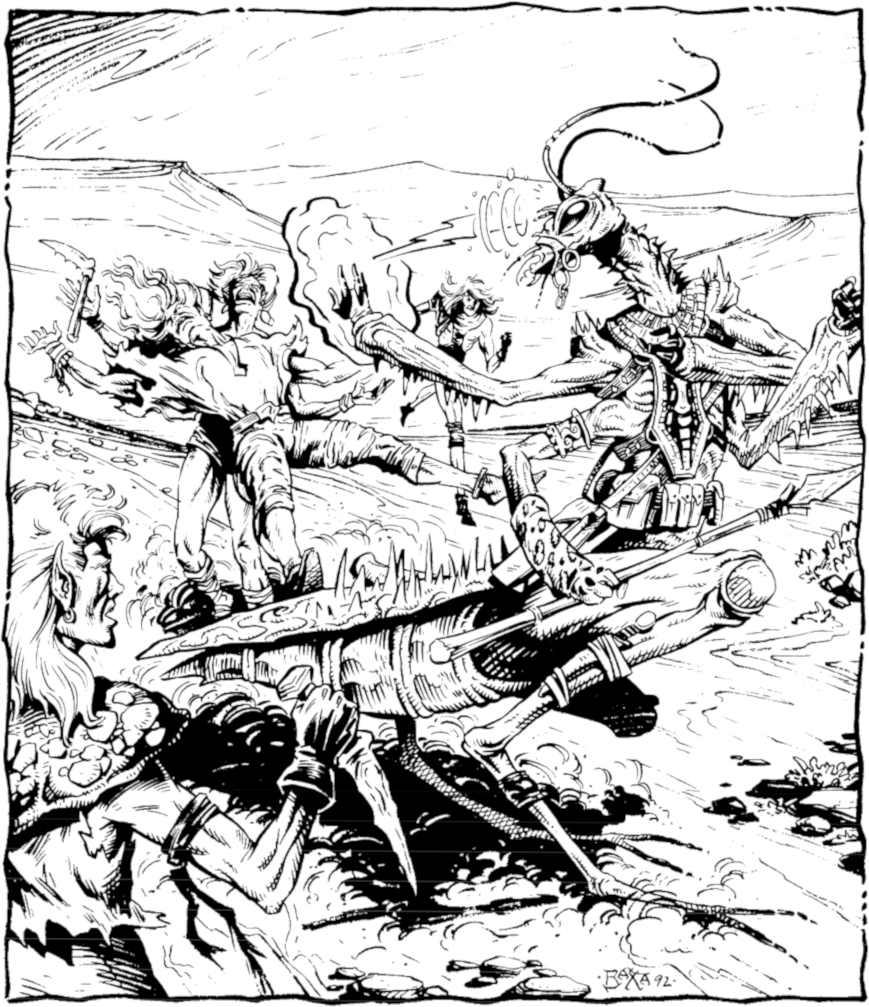
\includegraphics[width=\textwidth-1cm]{images/psywarrior-1.png}
\end{figure*}

\subsection{Making a Psychic Warrior}
Despite his spectacular combat powers, a psychic warrior is not a typical front-line combatant. Although a fighter, barbarian, or gladiator might swing a sword more accurately, or with greater force, a psychic warrior depends on his repertoire of power and feats. A psychic warrior is the psionic equivalent of an eldritch knight or a warmage from other settings. A psychic warrior's role in the party isn't easily defined, but his combination of physical might, the Way, and martial arts is useful in almost any encounter.

\textbf{Races:} Practicing psionics as part of hunting or combat comes as naturally to a Thri-kreen, as running comes to an elf. The Thri-kreen propensity to become ``chakak'' is rooted in the kreen ancestral memory. Becoming ``chakak'' is an almost unavoidable rite of kreen adulthood. Even kreen who focus their attentions in another class, such as the druid, tend to take at least one level as a psychic warrior. Nearly all pack-leaders and clutchleaders are accomplished chakak. Because of the clutch-mind, kreen chakak are far more cooperative, and infinitely less competitive with each other than the psychic warriors of other races.

Muls particularly excel as psychic warriors, as do humans, elves, and dwarves, to a lesser extent. Aarakocra and pterran psychic warriors are rare in those racial cultures, but individuals who take up the psychic warrior class tend to thrive. Halflings and jozhal psychic warriors are virtually unheard of.

\textbf{Alignment:} Psychic warriors tend towards neutrality with regards to good and evil, but they must be either lawful or chaotic. Chaotic psychic warriors, known commonly as ``mercenary psionicists,'' often work asattack thugs or assassins, though like bards, mercenary psionicists are notorious for switching allegiances according to the highest purse. Lawful psychic warriors, or ``mindguards,'' are the most sought-after personal guards for nobles and merchant lords. Like the elite rogue servants of the nobles, mindguards serve loyally in exchange for lavish compensation.

\subsection{Game Rule Information}

\textbf{Alignment:} Any lawful or chaotic.

\textbf{Hit Die:} d8.

\subsubsection{Class Skills}
\skill{Autohypnosis} (Wis), \skill{Climb} (Str), \skill{Concentration} (Con), \skill{Craft} (Int), \skill{Intimidate} (Cha), \skill{Jump} (Str), \skill{Knowledge} (psionics) (Int), \skill{Profession} (Wis), \skill{Ride} (Dex), and \skill{Search} (Int).

\textbf{Skill Points per Level:} 2 + Int modifier ($\times 4$ at 1st level).

\subsubsection{Class Features}

\textbf{Weapon and Armor Proficiency:} Psychic warriors are proficient with all simple and martial weapons, with all types of armor (heavy, medium, and light), and with shields (except tower shields).

\textbf{Power Points/Day:} A psychic warrior's ability to manifest powers is limited by the power points he has available. His base daily allotment of power points is given on \tabref{The Psychic Warrior}. In addition, he receives bonus power points per day if he has a high Wisdom score (see \tabref{Ability Scores and Bonus Power Points}). His race may also provide bonus power points per day, as may certain feats and items. A 1st-level psychic warrior gains no power points for his class level, but he gains bonus power points (if he is entitled to any), and can manifest the single power he knows with those power points.

\textbf{Powers Known:} A psychic warrior begins play knowing one psychic warrior power of your choice. Each time he achieves a new level, he unlocks the knowledge of a new power.

Choose the powers known from the psychic warrior power list. (Exception: The feat \feat{Expanded Knowledge} do allow a psychic warrior to learn powers from the lists of other classes.) A psychic warrior can manifest any power that has a power point cost equal to or lower than his manifester level.

The total number of powers a psychic warrior can manifest in a day is limited only by his daily power points.

A psychic warrior simply knows his powers; they are ingrained in his mind. He does not need to prepare them (in the way that some spellcasters prepare their spells), though he must get a good night's sleep each day to regain all his spent power points.

The Difficulty Class for saving throws against psychic warrior powers is 10 + the power's level + the psychic warrior's Wisdom modifier.

\textbf{Maximum Power Level Known:} A psychic warrior begins play with the ability to learn 1st-level powers. As he attains higher levels, he may gain the ability to master more complex powers.

To learn or manifest a power, a psychic warrior must have a Wisdom score of at least 10 + the power's level.

\textbf{Bonus Feats:} At 1st level, a psychic warrior gets a bonus combat-oriented feat in addition to the feat that any 1st level character gets and the bonus feat granted to a human character. The psychic warrior gains an additional bonus feat at 2nd level and every three levels thereafter (5th, 8th, 11th, 14th, 17th, and 20th). These bonus feats must be drawn from the feats noted as fighter bonus feats or psionic feats. The psychic warrior must still meet all prerequisites for the bonus feat, including ability score and base attack bonus minimums as well as class requirements. A psychic warrior cannot choose feats that specifically require levels in the fighter class unless he is a multiclass character with the requisite levels in the fighter class.

These bonus feats are in addition to the feats that a character of any class gains every three levels. A psychic warrior is not limited to fighter bonus feats and psionic feats when choosing these other feats.

\subsubsection{Ex-Psychic Warriors}
Any psychic warrior who ceases to be either lawful or chaotic, can no longer progress as a psychic warrior. She keeps all her powers known, power points, and bonus feats.

\subsection{Playing a Psychic Warrior}
When you mold your body and mind with the same rigor as a dwarf tempers his steel, no feat or combat prowess is beyond you. Through it all, you seek to understand the secret knowledge of combat, and how to take your nexus---a point in the center of your being where physical, mental, and spiritual energy can be harnessed---to the next level. You know the exact extent of your abilities and how hard it was to achieve them, so you are prone to showing it off flamboyantly, and claim to fear nothing.

Psychic warriors adventure for a plethora of reasons. Neither the religious fervor of an elemental cleric nor the glory of the fighter causes you to travel the Tablelands. More than faith, more than glory, you seek martial perfection. Whether you find that perfection in the cannibal-filled jungles of the Forest Ridge, in the choking silt of the Silt Sea, or in the den of the deadly braxat, you are driven to learn it and master it.

\subsubsection{Religion}
Religion might be entirely delusional to you, or you might find comfort in the elemental (or paraelemental) faiths, or even in the sorcerer-monarch of your city-state. If you are among the minority of psychic warriors who revere an element, you probably worship one associated with physical strength, such as Earth or Magma, or wisdom, such as Air or Sun.

\subsubsection{Other Classes}
Psychic warriors get along best with rogues, and to a lesser extent, fighters and bards. Generally, allies who show admiration for the psychic warriors' talents tend to get along well with the psychic warrior. Gladiators tend to get suspicious and envious of the psychic warrior's shows of unnatural and spectacular force, and many psychic warriors take a perverse pleasure in playing against the gladiator's jealousy, showing up the gladiator with spectacular stunts. Psychic warriors pretend to be indifferent to wizards, and to a lesser extent, psions, but many secretly envy the spectacle of a fireball.

\subsubsection{Combat}

You use your sword skills to defeat your foes as well as the limited access to manifest melee-oriented psionic powers. You have access to an amazing array of powerful combat feats. You have almost exclusive access to feats such as Deep Impact, Focused Sunder, and Wounding Attack, and you would do well to learn at least some of them. You have a limited selection of powers, so choose them carefully so you have a good mix of offensive, defensive and utility powers at your disposal.

\subsubsection{Advancement}
Your training began when you fought your way into an apprenticeship with a mentor---either a retired psychic warrior or an instructor in one of the many psionic academies dotting the Tablelands. You knew that finding that psychic warrior apprenticeship would not be that easy---that in fact, it would be an ordeal designed to test your body and mind to its fullest.

As a psychic warrior, your selection of psionic powers is paramount to your success. You might choose to focus on a specific psionic discipline, such as psychometabolism or psychokinesis, but learning a few powers from other disciplines is almost always advisable. True success in combat requires being ready for everything.

\subsection{Starting Packages}
\subsubsection{The Defender}

Mul Psychic Warrior

\textbf{Ability Scores:} Str 18, Dex 12, Con 15, Int 10, Wis 15, Cha 6.

\textbf{Skills:} \skill{Autohypnosis}, \skill{Concentration}, \skill{Intimidate}.

\textbf{Languages:} Common.

\textbf{Feat:} \feat{Combat Manifestation}.

\textbf{Weapons:} Great macahuitl (2d6/19--20)

Five javelins (1d6, 9 m).

\textbf{Armor:} Scale mail (+4 AC).

\textbf{Other Gear:} Standard adventurer's kit, 45 cp.

\subsubsection{The Destroyer}

Thri-kreen Psychic Warrior

\textbf{Ability Scores:} Str 17, Dex 17, Con 12, Int 8, Wis 16, Cha 4.

\textbf{Skills:} \skill{Concentration}, \skill{Intimidate}, \skill{Jump}.

\textbf{Languages:} Kreen.

\textbf{Feat:} \feat{Multiweapon Fighting}.

\textbf{Weapons:} Gythka (1d8/1d8)

Four chatkchas (1d6, 6 m).

\textbf{Armor:} Leather (+2 AC).

\textbf{Other Gear:} Standard adventurer's kit.

\subsubsection{The Skirmisher}

Human Psychic Warrior

\textbf{Ability Scores:} Str 14, Dex 13, Con 12, Int 10, Wis 15, Cha 8.

\textbf{Skills:} \skill{Concentration}, \skill{Intimidate}, \skill{Jump}, \skill{Psicraft}, \skill{Spot} (cc).

\textbf{Languages:} Common.

\textbf{Feat:} \feat{Dodge}, \feat{Weapon Focus} (glaive).

\textbf{Weapons:} Gouge (1d10/$\times$3)

Five javelins (1d6, 9 m).

\textbf{Armor:} Studded leather (+3 AC).

\textbf{Other Gear:} Standard adventurer's kit, 100 cp.

\subsection{Psychic Warriors on Athas}
\Quote{'Your studies have gone well, Turek,' he said quietly. 'You have learned the basics of psychic defense. It is time to practice your lessons.'

Turek nodded, his palms wet with sweat. He had known this was coming; he was one of the older students and it was time to begin his final studies before leaving the academy.

His master watched him without expression. Suddenly Turek found his attention ripped away from the patio and the master's physical form, being drawn inward. In his mind's eye a glowing sword appeared, poised to strike. 'I am the Sword', his master whispered. I pierce barriers and rend armor.' Turek swallowed nervously and summoned his defense. 'I am the Void, he thought over and over again. I cannot be found, I cannot be harmed.'

The Sword lunged forward, driving through the heart of the nothingness that cloaked Turek's presence...}{}

No place on Athas is safe from psionics. Armies and fortresses mean nothing to a master of the Way. To answer the threat of psionic attack, nobles and merchants retain the services of mercenary psionicists to guard against other users of the Way.

With a potential to advance in a number of different directions---offensive, defensive, support, and quick strike---psychic warriors make excellent additions to adventuring parties.

\subsubsection{Daily Life}

A psychic warrior spends the majority of his time perfecting his mind and body. The mental and spiritual demands of the Way require constant attention, so he can spare little time for carousing.

A psychic warrior with an apprentice spends much of his time training his student. A psychic warrior without one might or might not spend time seeking out one, according to his whims.

\subsubsection{Notables}

Hurgen Vurst, the half-giant garrison chief for Fort Harbeth is considered to be one of the most deadly specimens of his race, combining massive strength and a cleverness rarely found on half-giants. Chukaka the thri-kreen, was one of the first to be coin the term Kiltektet (the-learning-pack-who-enlightens), was a psychic warrior. Known as much for her wisdom, her teachings, as for her chatkchas, she is regarded by many the prototypical psychic warrior---serene, poised, and deadly.

\subsubsection{Organizations}

There is no specific organization that caters to psychic warriors. The Exalted Path (for males) and Serene Bliss (for females) orders in the city-state of Nibenay keep the city's ancient monastic tradition and they usually have several psychic warriors in their milieu. Villichi communities, female humans born with amazing psionic abilities, lie hidden in the deserts, harboring powerful psychic warriors.

\subsubsection{NPC Reactions}

As with fighters, individuals react to psychic warriors based on their previous interactions with other members of the class.

Gladiators have mixed feelings towards psychic warriors, they abilities can be of great value in the arena, but sometimes they feel a bit jealous of those abilities themselves, and they do not like other show offs competing for attention during gladiatorial matches. The only characters that psychic warriors as a rule will have an extremely hard time getting along with are other psychic warriors. Any party unfortunate enough to include more than one psychic warrior will be wrought with petty bickering, snide remarks, and endless competitions of spectacular force.

Merchants and nobles, on the other hand, greatly appreciate psychic warriors. They can always find ready employment as an elite mercenary, in the permanent guard of a noble family, or a merchant house sentry cadre.

\subsubsection{Psychic Warrior Lore}

Characters with ranks in \skill{Knowledge} (psionics) can research psychic warriors to learn more about them. When a character makes a skill check, read or paraphrase the following, including the information from lower DCs.

\textbf{DC 10:} A psychic warrior is a psionic sword-swinger who thinks he knows more about swordplay than anyone else.

\textbf{DC 15:} Like psions and wilders, psychic warrior walk the Unseen Way. Unlike them, psychic warriors train their bodies with the same rigor that they train their minds.

\textbf{DC 20:} Psychic warriors are strong, calm, and lethal. They gain the most psychic might of all those who study the Way.

\Class{Ranger}
{What you call monsters and beasts are simply other beings trying to survive in the wastelands. Some of them are just as desperate, lost, and confused as you are.}{Sudatu, elven scout}

The wastes of Athas are home to fierce and cunning creatures, from the bloodthirsty tembo to the malicious gaj. Because of that, Athasians have long learned how to adapt and survive even in the most inhospitable and savage environments.

One of the most cunning and powerful creatures of the wastes is the ranger, a skilled hunter and stalker. He knows his lands as if they were his home (as indeed they are); he knows his prey in deadly detail.

\HalfSpellcasterTable{The Ranger}{
1 & +1 & +2 & +2 & +0 & 1st favored enemy, Track, wild empathy &&&&\\
2 & +2 & +3 & +3 & +0 & Combat style &&&&\\
3 & +3 & +3 & +3 & +1 & Endurance &&&&\\
4 & +4 & +4 & +4 & +1 & Animal companion & 0 &&&\\
5 & +5 & +4 & +4 & +1 & 2nd favored enemy & 0 &&&\\
6 & +6/+1 & +5 & +5 & +2 & Improved combat style & 1 &&&\\
7 & +7/+2 & +5 & +5 & +2 & Woodland stride & 1 &&&\\
8 & +8/+3 & +6 & +6 & +2 & Swift tracker & 1 & 0 &&\\
9 & +9/+4 & +6 & +6 & +3 & Evasion & 1 & 0 &&\\
10 & +10/+5 & +7 & +7 & +3 & 3rd favored enemy & 1 & 1 &&\\
11 & +11/+6/+1 & +7 & +7 & +3 & Combat style mastery & 1 & 1 & 0 &\\
12 & +12/+7/+2 & +8 & +8 & +4 & & 1 & 1 & 1 &\\
13 & +13/+8/+3 & +8 & +8 & +4 & Camouflage & 1 & 1 & 1 &\\
14 & +14/+9/+4 & +9 & +9 & +4 & & 2 & 1 & 1 & 0 \\
15 & +15/+10/+5 & +9 & +9 & +5 & 4th favored enemy & 2 & 1 & 1 & 1 \\
16 & +16/+11/+6/+1 & +10 & +10 & +5 & & 2 & 2 & 1 & 1 \\
17 & +17/+12/+7/+2 & +10 & +10 & +5 & Hide in plain sight & 2 & 2 & 2 & 1 \\
18 & +18/+13/+8/+3 & +11 & +11 & +6 & & 3 & 2 & 2 & 1 \\
19 & +19/+14/+9/+4 & +11 & +11 & +6 & & 3 & 3 & 3 & 2 \\
20 & +20/+15/+10/+5 & +12 & +12 & +6 & 5th favored enemy & 3 & 3 & 3 & 3}


\subsection{Making a Ranger}
Rangers are capable in combat, although less so in open melee than the fighter, gladiator, or barbarian. His skills allow him to survive in the wilderness, to find his prey and to avoid detection. The ranger has the ability to gain special knowledge of certain types of creatures or lands. Knowledge of his enemies makes him more capable of finding and defeating those foes. Knowledge of terrain types or of specific favored lands makes it easier for him to live off the land, and makes it easier for him to take advantage of less knowledgeable foes. Rangers eventually learn to use the lesser spirits that inhabit Athas in order to produce spell-like effects. These lesser spirits inhabit small features of the land -- rocks, trees, cacti and the like.

These spirits are relatively powerless, and cannot manifest themselves. Their awareness is low, and their instincts are of the most primitive sort. The relationship between these lesser spirits and the creatures known as Spirits of the Land is unknown.

\textbf{Races:} As the race that carries the most fear and hatred of other races, and as the people with the richest land to protect, Halflings become rangers more commonly than any other race except for half-elves. Halflings are at home in their terrain (typically Forest Ridge or the Jagged Cliffs) and the ranger class teaches them the grace to move without detection, often to deadly effect. Their practice of cannibalism to emphasize their superiority over other sentient beings puts the ranger's tracking abilities to deadly use. Halfling rangers tend to take favored lands primarily, followed by favored enemy benefits. In the Forest Ridge, halfling rangers tend to pick pterrans and other neighboring races as favored enemies; rangers of the Jagged Cliffs tend to focus on bvanen, and kreen.

Elves frequently become rangers, serving as scouts and hunters for their tribes, but elves are not as naturally drawn to the wilderness as they are to magic. Half-elves are the race most compellingly drawn to the ranger class, since their isolation and natural gift with animals gives them a head start above rangers of other races. Half-Elven rangers sometimes seek to impress their Elven cousins with their desert skills, and when they are rejected, the wilderness often becomes the half-elf's only solace. A few half-elves turn to bitter hatred of the parent races that rejected them, and become merciless slave--hunters.

Although ranger skills do not come to naturally humans, their famous adaptability wins out in the end, and many humans make fine rangers. A few muls take up the ranger class while surviving in the wilderness after escaping slavery. Dwarves who become rangers find that their focus ability combines powerfully with the abilities of favored enemy and favored lands, but such characters rarely become adventurers since they tend to master wilderness skills in order to guard Dwarven communities.

Pterran rangers are common since rangers get along so well with the druidic and psionic leaders of the pterran villages. Aarakocra are similarly drawn to the ranger class to protect their villages from predators and enemies. Rangers are not unusual among the most hated humanoid races of Athas, such as gith, belgoi, and braxat. Among the various and dwindling communities of the wastes rangers are the most common character class.

\textbf{Alignment:} Rangers can be of any alignment, although they tend not to be lawful, preferring nature to civilization, silence to casual conversation, and ambush to meeting a foe boldly on the battlefield. Good rangers often serve as protectors of a village or of a wild area. In this capacity, rangers try to exterminate or drive off evil creatures that threaten the rangers' lands. Good rangers sometimes protect those who travel through the wilderness, serving sometimes as paid guides, but sometimes as unseen guardians. Neutral rangers tend to be wanderers and mercenaries, rarely tying themselves down to favored lands. The tracking and animal skills of rangers are well known in the World; virtually every trade caravan has at least one ranger scout or mekillot handler. Sometimes they stalk the land for vengeance, either for themselves or for an employer. Generally only evil rangers ply their skills in the slave trade. Other evil rangers seek to emulate nature's most fearsome predators, and take pride and pleasure in the terror that strangers take in their names.

\subsection{Game Rule Information}

\textbf{Hit Die:} d8.

\subsubsection{Class Skills}
\skill{Climb} (Str), \skill{Concentration} (Con), \skill{Craft} (Int), \skill{Handle Animal} (Cha), \skill{Heal} (Wis), \skill{Hide} (Dex), \skill{Jump} (Str), \skill{Knowledge} (dungeoneering) (Int), \skill{Knowledge} (geography) (Int), \skill{Knowledge} (nature) (Int), \skill{Listen} (Wis), \skill{Move Silently} (Dex), \skill{Profession} (Wis), \skill{Ride} (Dex), \skill{Search} (Int), \skill{Spot} (Wis), \skill{Survival} (Wis), and \skill{Use Rope} (Dex).

\textbf{Skill Points per Level:} 6 + Int modifier ($\times 4$ at 1st level).

\begin{figure*}[b!]
\centering
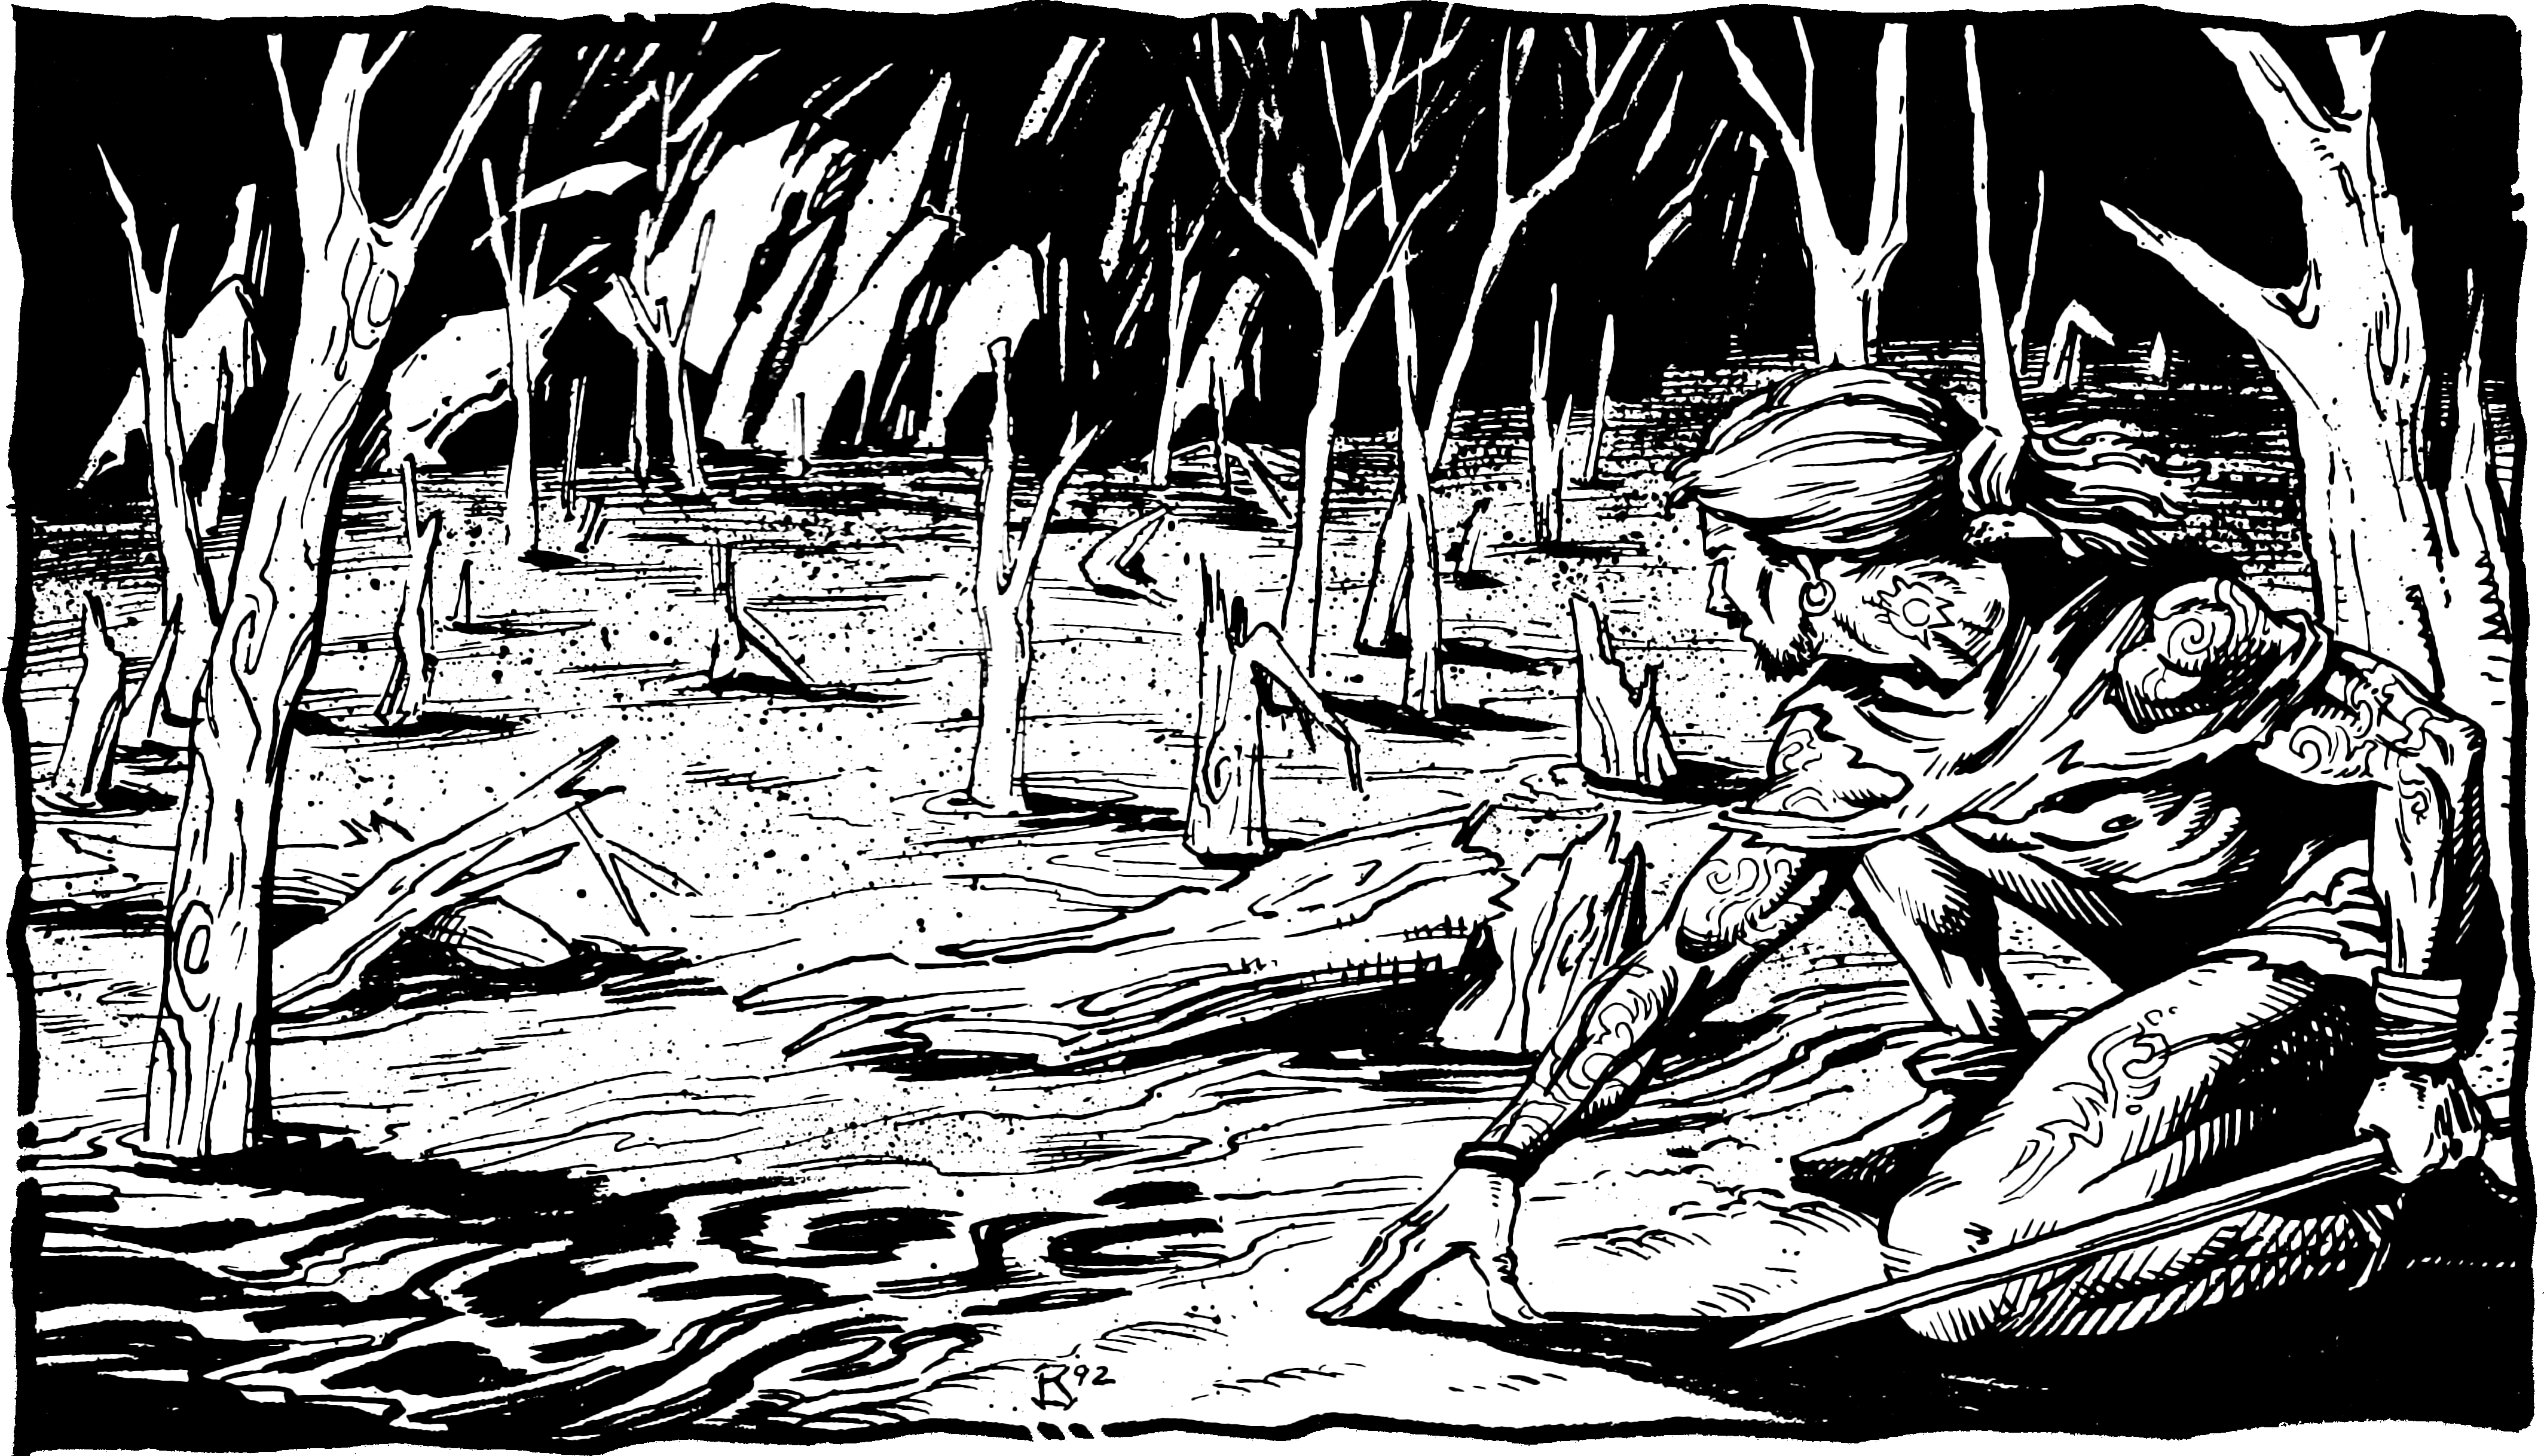
\includegraphics[width=\textwidth]{images/ranger-2.png}
\par\textit{\small\textcopyright Wizards of the Coast, 2020.}
\end{figure*}

\subsubsection{Class Features}
\textbf{Weapon and Armor Proficiency:} A ranger is proficient with all simple and martial weapons, and with light armor and shields (except tower shields).

\textbf{Favored Enemy (Ex):} At 1st level, a ranger may select a type of creature from among those given on \tabref{Athasian Favored Enemies}. The ranger gains a +2 bonus on \skill{Bluff}, \skill{Listen}, \skill{Sense Motive}, \skill{Spot}, and \skill{Survival} checks when using these skills against creatures of this type. Likewise, he gets a +2 bonus on weapon damage rolls against such creatures.

At 5th level and every five levels thereafter (10th, 15th, and 20th level), the ranger may select an additional favored enemy from those given on the table. In addition, at each such interval, the bonus against any one favored enemy (including the one just selected, if so desired) increases by 2.

If the ranger chooses humanoids or outsiders as a favored enemy, he must also choose an associated subtype, as indicated on the table. If a specific creature falls into more than one category of favored enemy, the ranger's bonuses do not stack; he simply uses whichever bonus is higher.

\Table{Athasian Favored Enemies}{X X}{
\tableheader Type (Subtype) & \tableheader Example\\
Aberration & gaj \\
Animal & lion \\
Construct & golem \\
Elemental (air) & air elemental beast \\
Elemental (earth) & crystal spider \\
Elemental (fire) & fire incarnation \\
Elemental (water) & rain paraelemental beast \\
Giant & beasthead giant \\
Humanoid (dwarf) & dwarf \\
Humanoid (elf) & elf \\
Humanoid (gith) & gith \\
Humanoid (halfling) & halfling \\
Humanoid (human) & human \\
Humanoid (jozhal) & jozhal \\
Humanoid (nikaal) & nikaal \\
Humanoid (psionic) & villichi \\
Humanoid (pterran) & pterran \\
Humanoid (reptilian) & silt runner \\
Humanoid (tarek) & tarek \\
Humanoid (tari) & tari \\
Magical beast & kirre \\
Monstrous humanoid & Thri-kreen \\
Outsider & silt half-elemental \\
Plant & hunting cactus \\
Undead & kaisharga \\
Vermin & kank}

\Table{Athasian Terrains}{X X}{
\tableheader Terrain Type & \tableheader Terrain Type\\
Boulder Field & Rocky Badland \\
Forest & Salt Flat \\
Jagged Cliffs & Sandy Waste \\
Mountain & Sea of Silt \\
Mud Flat & Stony Barren \\
Obsidian Waste & Swamp \\
Ocean & Verdant Belt}

\textbf{Favored Terrain (Ex):} At any time when a ranger could normally select a favored enemy, he may instead choose to select a favored terrain given on \tabref{Athasian Terrains}. A ranger receives a +2 bonus on \skill{Hide}, \skill{Listen}, \skill{Move Silently}, \skill{Search}, \skill{Spot} and \skill{Survival} checks made within your favored terrain. Likewise, he gets +2 bonus on \skill{Knowledge} (geography) and \skill{Knowledge} (nature) checks about your favored terrain.

This ability uses the same graduated progression that the favored enemy ability receives.

For example, at first level Sudatu selects monstrous humanoids as a favored enemy, receiving a +2 bonus when combating them. At fifth level, instead of taking a new favored enemy, he selects a Rocky Badlands as his favored terrain, and chooses to increase his favored enemy bonus to +4. At 10th level, Sudatu may again choose a new Favored Enemy, and may also choose between raising his favored enemy or favored terrain bonus by +2.

\textbf{Track:} A ranger gains \feat{Track} as a bonus feat.

\textbf{Wild Empathy (Ex):} A ranger can improve the attitude of an animal. This ability functions just like a \skill{Diplomacy} check to improve the attitude of a person. The ranger rolls 1d20 and adds his ranger level and his Charisma modifier to determine the wild empathy check result. The typical domestic animal has a starting attitude of indifferent, while wild animals are usually unfriendly.

To use wild empathy, the ranger and the animal must be able to study each other, which means that they must be within 9 meters of one another under normal visibility conditions. Generally, influencing an animal in this way takes 1 minute, but, as with influencing people, it might take more or less time.

The ranger can also use this ability to influence a magical beast with an Intelligence score of 1 or 2, but he takes a $-4$ penalty on the check.

\textbf{Combat Style (Ex):} At 2nd level, a ranger must select one of two combat styles to pursue: archery or two-weapon combat. This choice affects the character's class features but does not restrict his selection of feats or special abilities in any way.

If the ranger selects archery, he is treated as having the \feat{Rapid Shot} feat, even if he does not have the normal prerequisites for that feat.

If the ranger selects two-weapon combat, he is treated as having the \feat{Two-Weapon Fighting} feat, even if he does not have the normal prerequisites for that feat.

The benefits of the ranger's chosen style apply only when he wears light or no armor. He loses all benefits of his combat style when wearing medium or heavy armor.

\textbf{Endurance:} A ranger gains \feat{Endurance} as a bonus feat at 3rd level.

\textbf{Animal Companion (Ex):} At 4th level, a ranger gains an animal companion selected from the following list: badger, camel, dire rat, dog, riding dog, eagle, hawk, horse (light or heavy), owl, pony, snake (Small or Medium viper), or wolf. If the campaign takes place wholly or partly in an aquatic environment, the following creatures may be added to the ranger's list of options: manta ray, porpoise, Medium shark, and squid. This animal is a loyal companion that accompanies the ranger on his adventures as appropriate for its kind.

This ability functions like the druid ability of the same name, except that the ranger's effective druid level is one-half his ranger level. A ranger may select from the alternative lists of animal companions just as a druid can, though again his effective druid level is half his ranger level. Like a druid, a ranger cannot select an alternative animal if the choice would reduce his effective druid level below 1st.

\textbf{Spells:} Beginning at 4th level, a ranger gains the ability to cast a small number of divine spells, which are drawn from the ranger spell list. A ranger must choose and prepare his spells in advance (see below).

To prepare or cast a spell, a ranger must have a Wisdom score equal to at least 10 + the spell level. The Difficulty Class for a saving throw against a ranger's spell is 10 + the spell level + the ranger's Wisdom modifier.

Like other spellcasters, a ranger can cast only a certain number of spells of each spell level per day. His base daily spell allotment is given on \tabref{The Ranger}. In addition, he receives bonus spells per day if he has a high Wisdom score. When \tabref{The Ranger} indicates that the ranger gets 0 spells per day of a given spell level, he gains only the bonus spells he would be entitled to based on his Wisdom score for that spell level. The ranger does not have access to any domain spells or granted powers, as a cleric does.

A ranger prepares and casts spells the way a cleric does, though he cannot lose a prepared spell to cast a cure spell in its place. A ranger may prepare and cast any spell on the ranger spell list, provided that he can cast spells of that level, but he must choose which spells to prepare during his daily meditation.

Through 3rd level, a ranger has no caster level. At 4th level and higher, his caster level is one-half his ranger level.

\textbf{Improved Combat Style (Ex):} At 6th level, a ranger's aptitude in his chosen combat style (archery or two-weapon combat) improves. If he selected archery at 2nd level, he is treated as having the \feat{Manyshot} feat, even if he does not have the normal prerequisites for that feat.

If the ranger selected two-weapon combat at 2nd level, he is treated as having the \feat{Improved Two-Weapon Fighting} feat, even if he does not have the normal prerequisites for that feat.

As before, the benefits of the ranger's chosen style apply only when he wears light or no armor. He loses all benefits of his combat style when wearing medium or heavy armor.

\textbf{Woodland Stride (Ex):} Starting at 7th level, a ranger may move through any sort of undergrowth (such as natural thorns, briars, overgrown areas, and similar terrain) at his normal speed and without taking damage or suffering any other impairment.

However, thorns, briars, and overgrown areas that are enchanted or magically manipulated to impede motion still affect him.

\textbf{Swift Tracker (Ex):} Beginning at 8th level, a ranger can move at his normal speed while following tracks without taking the normal $-5$ penalty. He takes only a $-10$ penalty (instead of the normal $-20$) when moving at up to twice normal speed while tracking.

\textbf{Evasion (Ex):} At 9th level, a ranger can avoid even magical and unusual attacks with great agility. If he makes a successful Reflex saving throw against an attack that normally deals half damage on a successful save, he instead takes no damage. Evasion can be used only if the ranger is wearing light armor or no armor. A helpless ranger does not gain the benefit of evasion.

\textbf{Combat Style Mastery (Ex):} At 11th level, a ranger's aptitude in his chosen combat style (archery or two-weapon combat) improves again. If he selected archery at 2nd level, he is treated as having the \feat{Improved Precise Shot} feat, even if he does not have the normal prerequisites for that feat.

If the ranger selected two-weapon combat at 2nd level, he is treated as having the \feat{Greater Two-Weapon Fighting} feat, even if he does not have the normal prerequisites for that feat.

As before, the benefits of the ranger's chosen style apply only when he wears light or no armor. He loses all benefits of his combat style when wearing medium or heavy armor.

\textbf{Camouflage (Ex):} A ranger of 13th level or higher can use the \skill{Hide} skill in any sort of natural terrain, even if the terrain doesn't grant cover or concealment.

\textbf{Hide in Plain Sight (Ex):} While in any sort of natural terrain, a ranger of 17th level or higher can use the \skill{Hide} skill even while being observed.

\subsection{Playing a Ranger}

As a ranger, you nurture a close, almost mystical connection to the deadly terrain of Athas. To you, the burnt landscape is not a friend, but a well-respected adversary. Danger is always present, yet you understand it and even find a certain succor in living alongside it.

\subsubsection{Religion}

Many rangers pay homage to the elements, but a greater number honor the moons and the stars that guide them in the night---even though these celestial bodies do not have priests. In several city-states, particularly Gulg,
Kurn, and Eldaarich, many rangers owe fealty to the sorcerer-kings---virtually the entire noble caste of Gulg is comprised of rangers called judaga. Some rangers pay patronage to the Spirits of the Land, although these spirits do not bestow spells on rangers except those that multi-class as druid.

\subsubsection{Other Classes}

Rangers are slow to make friends with anyone, but have a particular affinity to druids, and to a lesser extent, barbarians and psions. Rangers tend not to lean on others for support and friendship, and often find it difficult to tolerate others who are quite different from themselves, such as talkative traders or controlling templars. Good rangers might simply try to avoid sharing a watch with a character that annoys them; neutral rangers tend to abandon annoying companions or just let them die; while evil rangers act friendly to the annoying companion and then slit their throat in their sleep.

Good rangers tend to hate defilers, although many rangers are ignorant of the distinction between preserving and defiling and hate wizards of all stripes. Strangely, many rangers have little objection to taking a companion who is of a favored enemy race, so long as that they are convinced that the companion is trustworthy and loyal.

\subsubsection{Combat}

Although you are a formidable warrior, you usually prefer not to stand against the sheer might of Athas' fighter, barbarians and gladiators. Your greatest ally is the environment itself. While in you favored terrain, you have a clear advantage over your adversaries. Try choosing favored enemies that are more common in your favored terrain.

As you advance, you are well served to invest in spells that have an effect other than dealing damage. If you can't drop a foe in one or two attacks, you can use entangle, snare, sting of the gold scorpion, or the like to make your opponents less dangerous in a prolonged fight.

\subsubsection{Advancement}

Perhaps the most dangerous place in Athas is inside a city-state: an environment rife with political intrigue, diseases, and assassination. To escape these noxious environs, you sought refuge in the wild where even the foulest elements of a society fear to tread. By gaining an intimate knowledge of this hazardous realm, you buy some breathing room and security from the urban madness.

As your ranger abilities increase, you find the Athasian wilderness a more and more inviting place (if a place with such constant peril can be called inviting). You can use your skills to establish safe havens for yourself or to gain employment opportunities---perhaps guiding a group of recently caught slaves through the Tyr valley or some noble into distant dangerous, location. You can also find that continuing to advance as a ranger or barbarian augments your already impressive abilities in the Athasian lands.

Continue to focus on skills such as Hive, Move Silently, and Survival. Spend discovered treasure on poison, magic weapons, and protective magic. The Mobility feat is good to consider, as is Nature's Child or Wastelander.

\subsection{Starting Packages}
\subsubsection{The Archer}
Elf Ranger

\textbf{Ability Scores:} Str 14, Dex 17, Con 10, Int 10, Wis 13, Cha 8.

\textbf{Skills:} \skill{Hide}, \skill{Listen}, \skill{Move Silently}, \skill{Spot}, \skill{Survival}.

\textbf{Languages:} Common, Elven.

\textbf{Feat:} \feat{Point Blank Shot}, \feat{Track}.

\textbf{Weapons:} Macahuitl (1d8/19--20)

Longbow with 20 arrows (1d8/$\times$3, 30 m).

\textbf{Armor:} Studded leather (+3 AC).

\textbf{Other Gear:} Standard adventurer's kit, 19 cp.

\subsubsection{The Scout}
Halfling Ranger

\textbf{Ability Scores:} Str 11, Dex 17, Con 12, Int 10, Wis 14, Cha 8.

\textbf{Skills:} \skill{Hide}, \skill{Knowledge} (nature), \skill{Listen}, \skill{Move Silently}, \skill{Spot}, \skill{Survival}.

\textbf{Languages:} Halfling.

\textbf{Feat:} \feat{Stealthy}, \feat{Track}.

\textbf{Weapons:} Macahuitl (1d6/19--20)

Small macahuitl (1d3/19--20)

Five javelins (1d4, 9 m).

\textbf{Armor:} Studded leather (+3 AC).

\textbf{Other Gear:} Standard adventurer's kit, 65 cp.

\subsubsection{The Wastelander}
Thri-kreen Ranger

\textbf{Ability Scores:} Str 14, Dex 19, Con 14, Int 8, Wis 15, Cha 4.

\textbf{Skills:} \skill{Hide}, \skill{Knowledge} (nature), \skill{Listen}, \skill{Move Silently}, \skill{Spot}, \skill{Survival}.

\textbf{Languages:} Kreen.

\textbf{Feat:} \feat{Track}, \feat{Wastelander}.

\textbf{Weapons:} Gythka (1d8/1d8)

Three chatkchas (1d6, 6 m).

\textbf{Armor:} Studded leather (+3 AC).

\textbf{Other Gear:} Standard adventurer's kit, 5 cp.

\subsection{Rangers on Athas}
\Quote{Trust me. He might not talk a lot and smell funnier than the rest of your men, but there is no other one I would bring along with me around the Great Ivory Plains.}{Waltian Inika, Gulg dune trader}

The Athasian wilderness is harsh and unforgiving, calling for skilled and capable men to master its ways---the ranger answers that challenge, living a rugged life through clever mastery of his surroundings. The ranger has a potent combination of stealth, woodcraft, magic, and fighting skill, making him the master of the wilderness.

\subsubsection{Daily Life}

A ranger adventures to learn about Athas, to protect nature, and to prove his superior hunting skills. Rangers spend their days in contemplation of nature, and tending their animal companions.

The Athasian ranger is a wanderer who hunts down a defiler to avenge himself for having his village destroyed, or a mercenary hunter for both monsters and humanoid creatures, or even a loner who simply prefers the company of animals.

\subsubsection{Notables}

Tales of halfling snipers are among the common Athasian legends. Any traveler to the Forest Ridge should rightfully fear the cannibals that move without a sound and strike without being seen. Thri-kreen are fabled for their rangers, as they are fast-moving relentless natural hunters, and their unarmed combat abilities become even more deadly when applied to subduing a quarry.

\subsubsection{Organizations}

There is no organized ranger organization; you are most likely to be a loner---or at best the leader of a group of raiders or renegades---than you are to gather with other rangers.

Often merchant houses are eager to employ you as a caravan guide through the most dangerous trade routes, or a city-state's templarate might hire you to provide a safe path to a templar patrol.

\subsubsection{NPC Reactions}

Within a city-state or large settlement, you find that you are either ignored or regarded with some small amount of curiosity. It is only after a city-dweller find himself outside the boundaries of his city-state that he truly appreciates you. Indeed, he holds you in the highest of regards, knowing that you are all that stands between him and a horrible death in the wastes.

\subsubsection{Ranger Lore}

Characters with ranks in \skill{Knowledge} (nature) can research rangers to learn more about them. When a character makes a skill check, read or paraphrase the following, including the information from lower DCs.

\textbf{DC 10:} Only those assisted by a ranger can hope to survive in the Athasian wilderness for long.

\textbf{DC 15:} Rangers move with ease through the harsh terrains that others find dangerous or impassable. They make of this aptitude to specialize in battling specific creatures of the wild.

\textbf{DC 20:} As a ranger advances in knowledge and skill, he grows more and more connected to the land, and eventually manages to draw spells from it.

\Class{Rogue}
{Marek, always helpful, said that the UnderTyr catacombs are supposed to be haunted. Think I'll go make some inquiries about where a 'heretic' like me can get some holy earth. Always go prepared...}{Janos, human rogue}

{\tableheader Dark Sun} offers a world of intrigue, manipulation, secret deals, and subtle treachery---in short, a rogue's playground. Rather than eking out their living at the
borders of society, many Athasian rogues dominate the action in many of the most powerful political factions in the Seven Cities: the Noble Houses, the templars, and the Merchant Houses. Often rogues themselves, the wealthy and powerful deploy lesser rogues as pawns in their endless games of acquisition, espionage, and deceit.

Individual rogues run the gamut of Athasian society, from the street rats of the cities to the vagabonds of the outlands, to the prosperous and respectable dune traders, to the low-ranking templars that search their caravans at the gates. Accomplished rogues are often sought by the nobility as agents, and can earn both wealth and honor in such positions---or earn a quick death should they be caught contemplating treachery against their masters.

\WarriorTable{The Rogue}{
1 & +0 & +0 & +2 & +0 & Sneak attack +1d6, trapfinding\\
2 & +1 & +0 & +3 & +0 & Evasion\\
3 & +2 & +1 & +3 & +1 & Sneak attack +2d6, trap sense +1\\
4 & +3 & +1 & +4 & +1 & Uncanny dodge\\
5 & +3 & +1 & +4 & +1 & Sneak attack +3d6\\
6 & +4 & +2 & +5 & +2 & Trap sense +2\\
7 & +5 & +2 & +5 & +2 & Sneak attack +4d6\\
8 & +6/+1 & +2 & +6 & +2 & Improved uncanny dodge\\
9 & +6/+1 & +3 & +6 & +3 & Sneak attack +5d6, trap sense +3\\
10 & +7/+2 & +3 & +7 & +3 & Special ability\\
11 & +8/+3 & +3 & +7 & +3 & Sneak attack +6d6\\
12 & +9/+4 & +4 & +8 & +4 & Trap sense +4\\
13 & +9/+4 & +4 & +8 & +4 & Sneak attack +7d6, special ability\\
14 & +10/+5 & +4 & +9 & +4 & \\
15 & +11/+6/+1 & +5 & +9 & +5 & Sneak attack +8d6, trap sense +5\\
16 & +12/+7/+2 & +5 & +10 & +5 & Special ability\\
17 & +12/+7/+2 & +5 & +10 & +5 & Sneak attack +9d6\\
18 & +13/+8/+3 & +6 & +11 & +6 & Trap sense +6\\
19 & +14/+9/+4 & +6 & +11 & +6 & Sneak attack +10d6, special ability\\
20 & +15/+10/+5 & +6 & +12 & +6 & }

\subsection{Making a Rogue}

A rogue can't stand up face to face with a mul warrior as well as a fighter or gladiator can. With his cunning and your various skills, however, he excels at taking the slightest opportunity and turning to his advantage. His ability to slip under the notice of an observer makes him a capable lone hunter, but his greatest strength are found through interaction with allies and foes, inside or outside, a battle---he can use his enemy`s slightest distraction to deliver a lethal blow, or ensure his party`s safe passage through a templar patrol.

\textbf{Races:} Elves, half-elves, and humans take to the rogue's skills and lifestyle with the greatest ease. Halflings, dwarves, and muls, while not commonly rogues, adapt to the class remarkably well when they take to it. Thri-kreen, pterrans, and aarakocra are usually quite adverse to the rogue class, and tend to do poorly. Half-giant rogues are unheard of except as fictional figures in comical tales around the fireside.

\textbf{Alignment:} Athasian rogues follow opportunity rather than ideals, but as many of them are lawful as chaotic. Lawful rogues tend to seek security and advancement in the service of nobles or in the ranks of the templars.

\subsection{Game Rule Information}
\textbf{Hit Die:} d6.

\subsubsection{Class Skills}
\skill{Appraise} (Int), \skill{Balance} (Dex), \skill{Bluff} (Cha), \skill{Climb} (Str), \skill{Craft} (Int), \skill{Decipher Script} (Int), \skill{Diplomacy} (Cha), \skill{Disable Device} (Int), \skill{Disguise} (Cha), \skill{Escape Artist} (Dex), \skill{Forgery} (Int), \skill{Gather Information} (Cha), \skill{Hide} (Dex), \skill{Intimidate} (Cha), \skill{Jump} (Str), \skill{Knowledge} (local) (Int), \skill{Listen} (Wis), \skill{Move Silently} (Dex), \skill{Open Lock} (Dex), \skill{Perform} (Cha), \skill{Profession} (Wis), \skill{Search} (Int), \skill{Sense Motive} (Wis), \skill{Sleight of Hand} (Dex), \skill{Spot} (Wis), \skill{Tumble} (Dex), \skill{Use Magic Device} (Cha), \skill{Use Psionic Device} (Cha), and \skill{Use Rope} (Dex).

\textbf{Skill Points per Level:} 8 + Int modifier ($\times4$ at 1st level).

\subsubsection{Class Features}
\textbf{Weapon and Armor Proficiency:} Rogues are proficient with all simple weapons, plus the bard's friend, blowgun, garrote, hand crossbow, rapier, sap, shortbow, short sword, small macahuitl, tonfa, widow's knife, and wrist razor. Rogues are proficient with light armor, but not with shields.

\textbf{Sneak Attack:} If a rogue can catch an opponent when he is unable to defend himself effectively from her attack, she can strike a vital spot for extra damage.

The rogue's attack deals extra damage any time her target would be denied a Dexterity bonus to AC (whether the target actually has a Dexterity bonus or not), or when the rogue flanks her target. This extra damage is 1d6 at 1st level, and it increases by 1d6 every two rogue levels thereafter. Should the rogue score a critical hit with a sneak attack, this extra damage is not multiplied.

Ranged attacks can count as sneak attacks only if the target is within 9 meters.

With a sap (blackjack) or an unarmed strike, a rogue can make a sneak attack that deals nonlethal damage instead of lethal damage. She cannot use a weapon that deals lethal damage to deal nonlethal damage in a sneak attack, not even with the usual $-4$ penalty.

A rogue can sneak attack only living creatures with discernible anatomies---undead, constructs, oozes, plants, and incorporeal creatures lack vital areas to attack. Any creature that is immune to critical hits is not vulnerable to sneak attacks. The rogue must be able to see the target well enough to pick out a vital spot and must be able to reach such a spot. A rogue cannot sneak attack while striking a creature with concealment or striking the limbs of a creature whose vitals are beyond reach.

\textbf{Trapfinding:} Rogues (and only rogues) can use the Search skill to locate traps when the task has a Difficulty Class higher than 20.

Finding a nonmagical trap has a DC of at least 20, or higher if it is well hidden. Finding a magic trap has a DC of 25 + the level of the spell used to create it.

Rogues (and only rogues) can use the \skill{Disable Device} skill to disarm magic traps. A magic trap generally has a DC of 25 + the level of the spell used to create it.

A rogue who beats a trap's DC by 10 or more with a \skill{Disable Device} check can study a trap, figure out how it works, and bypass it (with her party) without disarming it.

\textbf{Evasion (Ex):} At 2nd level and higher, a rogue can avoid even magical and unusual attacks with great agility. If she makes a successful Reflex saving throw against an attack that normally deals half damage on a successful save, she instead takes no damage. Evasion can be used only if the rogue is wearing light armor or no armor. A helpless rogue does not gain the benefit of evasion.

\textbf{Trap Sense (Ex):} At 3rd level, a rogue gains an intuitive sense that alerts her to danger from traps, giving her a +1 bonus on Reflex saves made to avoid traps and a +1 dodge bonus to AC against attacks made by traps. These bonuses rise to +2 when the rogue reaches 6th level, to +3 when she reaches 9th level, to +4 when she reaches 12th level, to +5 at 15th, and to +6 at 18th level.

Trap sense bonuses gained from multiple classes stack.

\textbf{Uncanny Dodge (Ex):} Starting at 4th level, a rogue can react to danger before her senses would normally allow her to do so. She retains her Dexterity bonus to AC (if any) even if she is caught flat-footed or struck by an invisible attacker. However, she still loses her Dexterity bonus to AC if immobilized.

If a rogue already has uncanny dodge from a different class she automatically gains improved uncanny dodge instead.

\textbf{Improved Uncanny Dodge (Ex):} A rogue of 8th level or higher can no longer be flanked.

This defense denies another rogue the ability to sneak attack the character by flanking her, unless the attacker has at least four more rogue levels than the target does.

If a character already has uncanny dodge from a second class, the character automatically gains improved uncanny dodge instead, and the levels from the classes that grant uncanny dodge stack to determine the minimum rogue level required to flank the character.

\textbf{Special Abilities:} On attaining 10th level, and at every three levels thereafter (13th, 16th, and 19th), a rogue gains a special ability of her choice from among the following options.

\textit{Crippling Strike (Ex):} A rogue with this ability can sneak attack opponents with such precision that her blows weaken and hamper them. An opponent damaged by one of her sneak attacks also takes 2 points of Strength damage. Ability points lost to damage return on their own at the rate of 1 point per day for each damaged ability.

\textit{Defensive Roll (Ex):} The rogue can roll with a potentially lethal blow to take less damage from it than she otherwise would. Once per day, when she would be reduced to 0 or fewer hit points by damage in combat (from a weapon or other blow, not a spell or special ability), the rogue can attempt to roll with the damage. To use this ability, the rogue must attempt a Reflex saving throw (DC = damage dealt). If the save succeeds, she takes only half damage from the blow; if it fails, she takes full damage. She must be aware of the attack and able to react to it in order to execute her defensive roll---if she is denied her Dexterity bonus to AC, she can't use this ability. Since this effect would not normally allow a character to make a Reflex save for half damage, the rogue's evasion ability does not apply to the defensive roll.

\textit{Dune Trader:} You gain +4 competence bonus to \skill{Diplomacy} checks with regard to buying or selling goods. Furthermore, \skill{Speak Language} becomes a class skill.

\textit{False Vulnerability (Ex):} While lying prone, you are not as helpless as you appear. Opponents do not get +4 to hit you while you are prone, and you can ``kip up,'' or leap from a prone position as a free action. You do not provoke an attack of opportunity when standing up. If this ability is used with a feint action, you get a +4 circumstance bonus to your opposed Bluff roll.

\textit{Improved Evasion (Ex):} This ability works like evasion, except that while the rogue still takes no damage on a successful Reflex saving throw against attacks henceforth she takes only half damage on a failed save. A helpless rogue does not gain the benefit of improved evasion.

\textit{Looter's Luck (Ex):} You can use your \skill{Appraise} skill to instinctively identify the most valuable item in a pile of loot as a move action. The DC for this accomplishment is DC 10 + the number of items in the selection. If you cannot see the items that you are choosing from (e.g. you are trying to pickpocket someone), then a full-round action is required, and the DC rises to 15 + the number of items.

\textit{Notoriety:} The fame of your exploits precedes you in the Seven Cities; you gain +4 to all \skill{Intimidate} and \skill{Bluff} checks. Adventurers seek your fellowship; you receive a +4 to your Leadership score if you have the \feat{Leadership} feat.

\textit{Opportunist (Ex):} Once per round, the rogue can make an attack of opportunity against an opponent who has just been struck for damage in melee by another character. This attack counts as the rogue's attack of opportunity for that round. Even a rogue with the \feat{Combat Reflexes} feat can't use the opportunist ability more than once per round.

\textit{Silver Tongue (Ex):} Your constant dealing with others gives you a keen sense of how to make them believe your lies. You may attempt a retry of the Bluff skill, but with a $-5$ penalty. This ability also gives you a +2 bonus to your \skill{Disguise} skill.

\textit{Skill Mastery:} The rogue becomes so certain in the use of certain skills that she can use them reliably even under adverse conditions.

Upon gaining this ability, she selects a number of skills equal to 3 + her Intelligence modifier. When making a skill check with one of these skills, she may take 10 even if stress and distractions would normally prevent her from doing so. A rogue may gain this special ability multiple times, selecting additional skills for it to apply to each time.

\textit{Slippery Mind (Ex):} This ability represents the rogue's ability to wriggle free from magical effects that would otherwise control or compel her. If a rogue with slippery mind is affected by an enchantment spell or effect and fails her saving throw, she can attempt it again 1 round later at the same DC. She gets only this one extra chance to succeed on her saving throw.

\textit{Feat:} A rogue may gain a bonus feat in place of a special ability.

\subsection{Playing a Rogue}

Rogues run the gamut of society. Athasian rogues range from gutter snipes who prey upon the merchants and free citizens of the cities to vagabonds who steal what they can from passing caravans or merchant trains. At their best, rogues can be in the employ of the nobility, plying their trade by contract in the name of a royal household, or they can be men or women of principle and honor who steal only from the corrupt and wealthy.

There is no thieves' guild on Athasian cities. However, most Athasians rogues attempt to attract a patron. A patron is a noble or senior templar who will sponsor the rogue and protect him under his house and name. The rogue is then expected to perform certain tasks for his new master in return---including theft, spying, and even assassination.

You might adventure because you desire excitement. Someone with your smarts get bored with ordinary pursuits. Alternatively, you might have set off a life of adventure after your big heist or some political manipulation gone wrong. For some reason, you have to keep moving, and a life of adventure offers you a regular change of scenery.

All seek to exercise their abilities to grow to even greater levels of power. You are clever enough to know that there's always more to learn. Although you tend to be (dangerously) self-reliant, you understand the value of having ``friends'' and allies in your pursuits, so try to not entangle them in your web of lies and trickery until you no longer need them.

\subsubsection{Religion}

Although they are as superstitious as the next Athasian, rogues are not known for their devotion or piety. Chaotic rogues tend to get along best with religions associated with elemental air.

\subsubsection{Other Classes}

Rogues enjoy working with members of other classes so long as their own skills and are valued and treated with respect. On Athas, rogue is as honorable a profession as any other, and more honorable than some (such as
wizard), and they mark for enmity anyone who describes them as a common thief.

\subsubsection{Combat}

You are at your best when you catch foes unaware. Use your skills to hide ourself so that you can employ surprise tactics. In melee, move into flanking position or use the Bluff skill to feint in combat and drop a powerful sneak attack.

\subsubsection{Advancement}

You should assign your various skills points according to your role in your adventuring group. If the group already has someone who is good at finding traps and sneaking about, boost your ranks in social skills such as Diplomacy and Gather Information. High bonuses in Bluff and Move Silently are a must if you're going to use your sneak attacks often.

You have many good options for feats, but be sure to take Combat Expertise and Improved Feint to get the most out of your sneak attacks. If you are interested in having a lot of feats, it might be worthwhile to take a level of psychic warrior, since the first level of psychic warrior gives you proficiency with all types of armor, a bonus feat you could use for Combat Expertise or Improved Feint, and a psionic power you could use to boost your rogue skills. If you are the social type, consider becoming a dune trader (page 90).

\subsection{Starting Packages}
\subsubsection{The Archer}
Half-Elf Rogue

\textbf{Ability Scores:} Str 8, Dex 17, Con 12, Int 13, Wis 14, Cha 8.

\textbf{Skills:} \skill{Climb}, \skill{Disable Device}, \skill{Hide}, \skill{Listen}, \skill{Move Silently}, \skill{Open Lock}, \skill{Search}, \skill{Spot}, \skill{Tumble}.

\textbf{Languages:} Common.

\textbf{Feat:} \feat{Point Blank Shot}.

\textbf{Weapons:} Wrist razor (1d6/18--20)

Shortbow with 20 arrows (1d6/$\times$3, 18 m).

\textbf{Armor:} Studded leather (+3 AC).

\textbf{Other Gear:} Standard adventurer's kit, thieves' tools, 29 cp.

\subsubsection{The Knife in the Dark}
Elf Rogue

\textbf{Ability Scores:} Str 13, Dex 17, Con 10, Int 10, Wis 14, Cha 8.

\textbf{Skills:} \skill{Balance}, \skill{Bluff}, \skill{Disable Device}, \skill{Hide}, \skill{Listen}, \skill{Move Silently}, \skill{Open Lock}, \skill{Search}, \skill{Spot}, \skill{Tumble}.

\textbf{Languages:} Elven, Common.

\textbf{Feat:} \feat{Stealthy}.

\textbf{Weapons:} Macahuitl (1d8/19--20)

Tonfa (1d4)

Shortbow with 20 arrows (1d6/$\times$3, 18 m).

\textbf{Armor:} Studded leather (+3 AC).

\textbf{Other Gear:} Standard adventurer's kit, thieves' tools, 5 cp.

\subsubsection{The Trader}
Human Rogue

\textbf{Ability Scores:} Str 8, Dex 15, Con 10, Int 13, Wis 12, Cha 14.

\textbf{Skills:} \skill{Appraise}, \skill{Bluff}, \skill{Diplomacy}, \skill{Forgery}, \skill{Gather Information}, \skill{Knowledge} (local), \skill{Profession}, \skill{Sense Motive}, \skill{Speak Language} (cc).

\textbf{Languages:} Common.

\textbf{Feat:} \feat{Combat Reflexes}, \feat{Trader}.

\textbf{Weapons:} Longspear (1d8/$\times$3)

Wrist razor (1d6/18--20)

Light crossbow with 20 bolts (1d8/19--20, 24 m).

\textbf{Armor:} Studded leather (+3 AC).

\textbf{Other Gear:} Standard adventurer's kit, thieves' tools, 14 cp.

\subsection{Rogues on Athas}
\Quote{Going on personal experience, my one piece of advice to you is this--never trust anything with pointy ears. It'll either cheat you or try to eat you.}{Marek, human trader}

The rogue class gives a player a chance to play the archetypical trickster or scoundrel. Rogues also make great villains. By manipulating NPCs and situations the PCs encounter, or by being employed by a rival noble, an evil rogue can operate behind the scenes and trick the adventurers to his own ends.

\subsubsection{Daily Life}
The way a rogue behaves depends largely on his sense of morality. Some think nothing of adopting false identities or working as assassins for their noble patrons in exchange for silver, relying on their skills and charms to get through anything. A few other rogues find themselves driven to use their powers to help people.

\subsubsection{Notables}
The human Ramphion is the current leader of the Balican Veiled Alliance and has held the position for thirteen years, managing to rise to his title through sheer force of personality and charisma albeit not being able to cast even the simplest of cantrips. All trade lords are accomplished rogues. Master Sintha Valex is one of those, owner of large warehouses in Tyr. Frequently small quantities of the raw material are ``seeming lost'' in the warehouse, and end up being sold by Sintha to outgoing caravans to be sold in other cities of the Tablelands.

\subsubsection{Organizations}
Rogues don't organize together, but they often linger around the same places, such as the Bard's Quarter, the Elven Quarter, or Merchant House's Emporiums. A rogue joining an organization probably has a specific goal (or target) in mind and rakes a position that best allows him to attain it. A long-term commitment to such a group rarely appeals to a rogue.

\subsubsection{NPC Reactions}
Rogues make a good job about hiding their true motives and identities. Individuals who know about a rogue's true colors begin with an attitude one step more hostile than normal. Lawful clerics and templars in particular look poorly upon rogues, as does anyone who puts importance in forthrightness.

\subsubsection{Rogue Lore}
Characters with ranks in \skill{Knowledge} (local) can research rogues to learn more about them. When a character makes a skill check, read or paraphrase the following, including the information from lower DCs.

\textbf{DC 10:} Rogues are opportunists and tricksters. They employ deception and quick reflexes to get what they want.

\textbf{DC 15:} Rogues don't fight fair, if they fight at all, and their tongues are just as dangerous as their poisonous daggers.

\textbf{DC 20:} Rogues are adept at striking at vital spots when their targets are distracted, and their reflexes are quick enough to dodge most magical attacks.
\Class{Templar}
{Against the law? The law is a convenience, a tool for us to use as we will, not a yoke bound to our necks. Laws are guidelines, not rules cast in iron. Stretching them is not the same as breaking them, my young apprentice. Take that to heart, for if you accuse me again, I will have your heart served cold.}{Zelgado De'Draigee, human templar}

Templars are civil servants within a city-state's government organization commonly referred to as a ``temple,'' ``bureau,'' or ``order.'' Each templar swears obedience to his temple, and absolute fealty to his sorcerer-king. In return, the sorcerer-king grants them spell power stolen from the elemental planes.

In most city-states, templars are the ultimate authority---judge, jury, and executioner. Templars police and administer the city-states, and serve other civil roles ranging from general to jailor and from tax collector to garbage collector.

\SpellcasterTable{4mm}{The Templar}{
\SpellHeader{9} \\
1  & +0         & +2  & +0 & +2  & Assume domain, secular aptitude, sigil & 5 & 3+1 &&&&&&&&\\
2  & +1         & +3  & +0 & +3  &                                        & 6 & 4+1 &&&&&&&&\\
3  & +2         & +3  & +1 & +3  &                                        & 6 & 5+1 &&&&&&&&\\
4  & +3         & +4  & +1 & +4  & Turn or rebuke undead                  & 6 & 6+1 & 3+1 &&&&&&&\\
5  & +3         & +4  & +1 & +4  &                                        & 6 & 6+1 & 4+1 &&&&&&&\\
6  & +4         & +5  & +2 & +5  & \feat{Scribe Scroll}                   & 6 & 6+1 & 5+1 & 3+1 &&&&&&\\
7  & +5         & +5  & +2 & +5  &                                        & 6 & 6+1 & 6+1 & 4+1 &&&&&&\\
8  & +6/+1      & +6  & +2 & +6  & \feat{Brew Potion}                     & 6 & 6+1 & 6+1 & 5+1 & 3+1 &&&&&\\
9  & +6/+1      & +6  & +3 & +6  &                                        & 6 & 6+1 & 6+1 & 6+1 & 4+1 &&&&&\\
10 & +7/+2      & +7  & +3 & +7  &                                        & 6 & 6+1 & 6+1 & 6+1 & 5+1 & 3+1 &&&&\\
11 & +8/+3      & +7  & +3 & +7  &                                        & 6 & 6+1 & 6+1 & 6+1 & 6+1 & 4+1 &&&&\\
12 & +9/+4      & +8  & +4 & +8  &                                        & 6 & 6+1 & 6+1 & 6+1 & 6+1 & 5+1 & 3+1 &&&\\
13 & +9/+4      & +8  & +4 & +8  &                                        & 6 & 6+1 & 6+1 & 6+1 & 6+1 & 6+1 & 4+1 &&&\\
14 & +10/+5     & +9  & +4 & +9  &                                        & 6 & 6+1 & 6+1 & 6+1 & 6+1 & 6+1 & 5+1 & 3+1 &&\\
15 & +11/+6/+1  & +9  & +5 & +9  &                                        & 6 & 6+1 & 6+1 & 6+1 & 6+1 & 6+1 & 6+1 & 4+1 &&\\
16 & +12/+7/+2  & +10 & +5 & +10 &                                        & 6 & 6+1 & 6+1 & 6+1 & 6+1 & 6+1 & 6+1 & 5+1 & 3+1 &\\
17 & +12/+7/+2  & +10 & +5 & +10 &                                        & 6 & 6+1 & 6+1 & 6+1 & 6+1 & 6+1 & 6+1 & 6+1 & 4+1 &\\
18 & +13/+8/+3  & +11 & +6 & +11 &                                        & 6 & 6+1 & 6+1 & 6+1 & 6+1 & 6+1 & 6+1 & 6+1 & 5+1 & 3+1 \\
19 & +14/+9/+4  & +11 & +6 & +11 &                                        & 6 & 6+1 & 6+1 & 6+1 & 6+1 & 6+1 & 6+1 & 6+1 & 6+1 & 4+1 \\
20 & +15/+10/+5 & +12 & +6 & +12 &                                        & 6 & 6+1 & 6+1 & 6+1 & 6+1 & 6+1 & 6+1 & 6+1 & 6+1 & 5+1
}
\begin{figure}[t!]
\centering
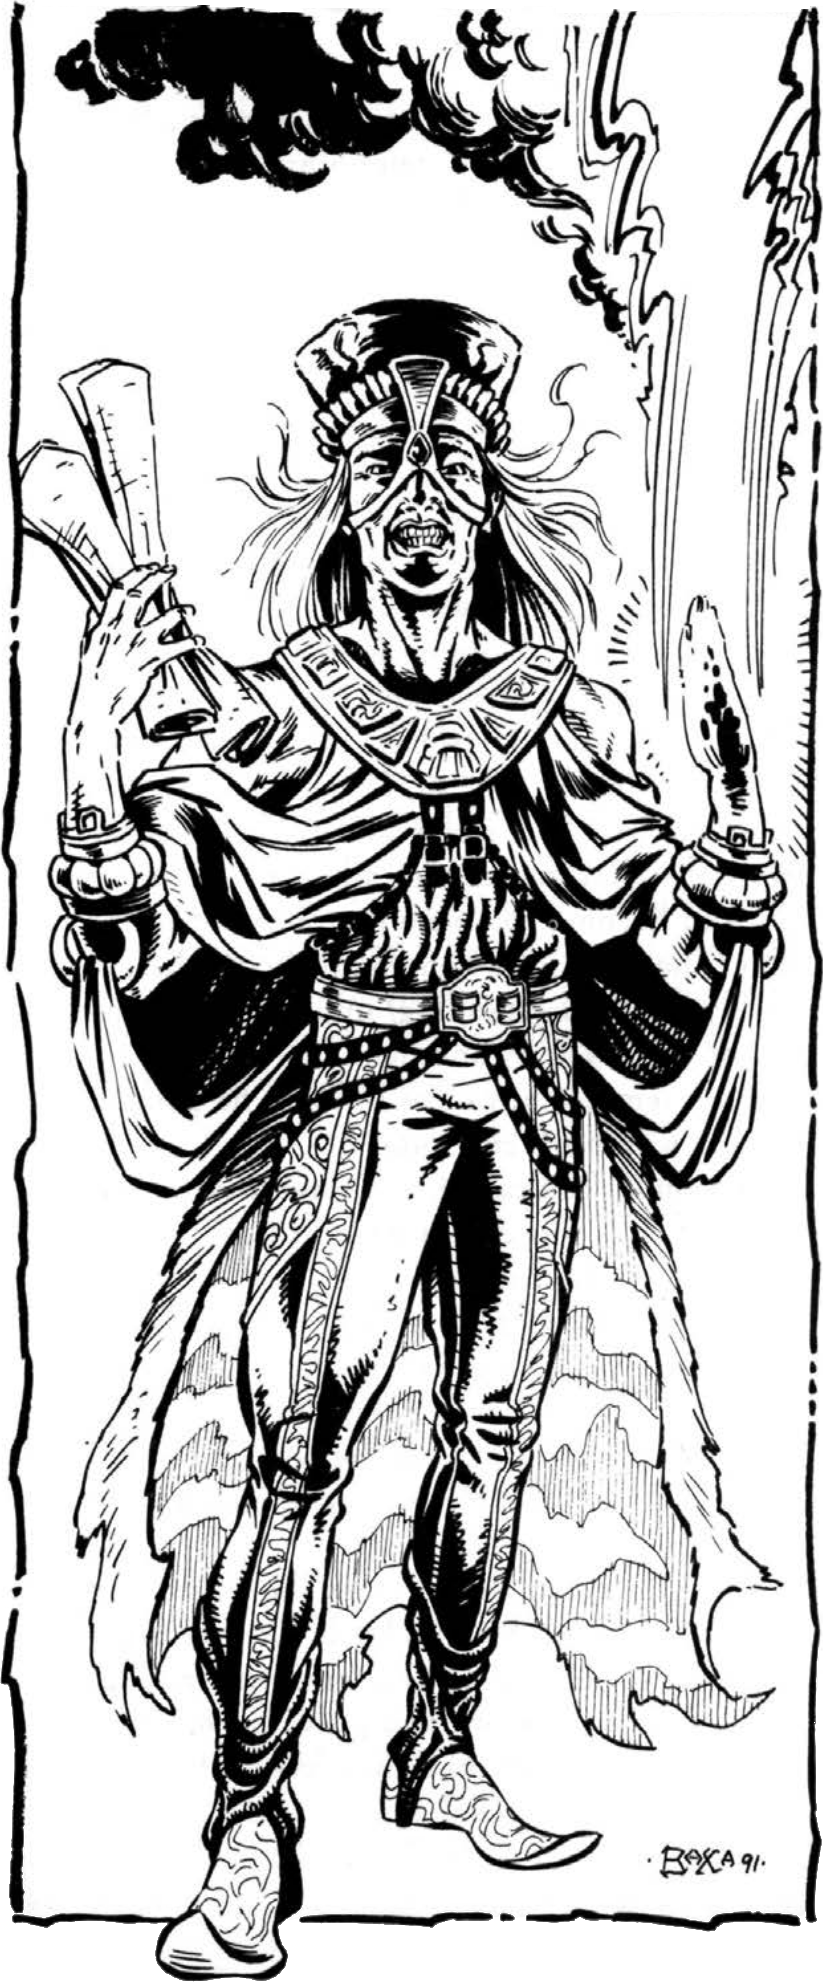
\includegraphics[width=\columnwidth]{images/templar-1.png}
\WOTC
\end{figure}

\subsection{Making a Templar}
Templars can cast a number of divine spells each day, as granted by their lord. If necessary they can be a destructive fighting force, but they serve much better as officers of slave-soldiers, mercenaries, or undead. Their wide array of available skills reflects the equally wide array of roles that Templars fill as servants of the sorcerer-kings and queens.

\textbf{Abilities:} If you want to make good use of your templar spells and you secular aptitude, you'll need a high Charisma. As with any melee-oriented class, Strength is a key ability for templars and Constitution provides you with increased ht points as usual.

\textbf{Races:} While the need for religion and divine magic is nearly universal on Athas, the need for specialized militant priest--bureaucrats is peculiar to large city-states dominated by sorcerer-kings. While in theory, no sentient race is precluded from the templar class, in practice, a sorcerer-king grant spells only to those who he wants to represent him. Humans dominate the templar priesthoods of all city-states except for New Giustenal. Dwarves, muls, and half-elves commonly become templars in many cities, while elves are less commonly accepted. Templars of other races are rare or unheard--of in most cities.

\textbf{Alignment:} A templar's alignment must be within one step of his sorcerer-king's (that is, it may be one step away on either the lawful--chaotic axis or the good--evil axis, but not both). Because of that, templars are almost never good. The laws they uphold are corrupt; the monarchs they serve are arguably the vilest creatures on the face of Athas, and often the templars are cruel and unjust themselves. However, many templars take considerable pride in the prosperity and magnificence of their city-state, and in the well--oiled machine of their order. Templars are most commonly lawful neutral or lawful evil.

\subsection{Game Rule Information}

\textbf{Alignment:} A templar's alignment must be within one step of his sorcerer-monarch's in each axis (that is, it may be one step away on the lawful-chaotic axis or the good-evil axis, but not two steps in either of them). A cleric may not be neutral unless his sorcerer-monarch's alignment is also neutral.

\textbf{Hit Die:} d8.

\subsubsection{Class Skills}
\skill{Appraise} (Int), \skill{Bluff} (Cha), \skill{Concentration} (Con), \skill{Craft} (Int), \skill{Diplomacy} (Cha), \skill{Forgery} (Int), \skill{Gather Information} (Cha), \skill{Heal} (Wis), \skill{Intimidate} (Cha), \skill{Knowledge} (all skills individually) (Int), \skill{Literacy} (N/A), \skill{Profession} (Wis), \skill{Sense Motive} (Wis), \skill{Spellcraft} (Int), and \skill{Spot} (Wis).

\textbf{Skill Points per Level:} 4 + Int modifier ($\times 4$ at 1st level).

\subsubsection{Class Features}

\textbf{Weapon and Armor Proficiency:} Templars are proficient in all simple weapons. Since templar training involves some education in warfare, templars receive two martial weapons proficiencies. Templars are proficient in light and medium armor and shields (except tower shields).

\textbf{Spellcasting:} A templar casts divine spells, which are drawn from the templar spell list. When she gain access to a new level of spells, she automatically knows all the spells for that level on the templar's spell list. She can cast any spell she know without preparing it ahead of time. Essentially, her spell list is the same as her spells known list.

To cast a spell, a templar must have a Charisma score of 10 + the spell's level. The Difficulty Class for a saving throw against a templar's spell is 10 + the spell's level + the templar's Cha modifier. Like other spellcasters, a templar can cast only a certain number of spells of each level per day. The base daily allotment is given on \tabref{The Templar}. In addition, she receives bonus spells if she has a high Charisma score.

She can also cast one domain spell of each spell level per day, as a cleric does. The domain spell is chosen at the time of casting from the spells associated with your assumed domains (see below), as she casts spells spontaneously and need not prepare spells ahead of time.

A templar need not prepare spells in advance. She can cast any spell she knows at any time, assuming she has not yet used up your spells per day for that spell level.

Templars use their sorcerer-king's sigil as divine focus.

\textbf{Assume Domain:} A templar is assigned two domains based on her sorcerer-monarch. Each domain gives her access to a domain spell at each spell level she can cast, from 1st on up, as well as a granted power. She gets the granted powers of both the assumed domains. With access to two domain spells at a given spell level, she adds only one of those spells to your spells known list.

\Table{Sorcerer-Kings' Domains and Alignment}{l X l}{
\tableheader Sorcerer-Monarch & \tableheader Domains & \tableheader Alignment\\
Abalach-Re & Chaos, Charm & Chaotic Evil \\
Andropinis & Law, Nobility & Neutral Evil \\
Borys & Destruction, Protection & Lawful Evil \\
Daskinor & Chaos, Madness & Lawful Evil \\
Dregoth & Death, Destruction & Chaotic Evil \\
Hamanu & Strength, War$\dagger$ & Neutral Evil \\
Kalak & Magic, Trickery & Neutral Evil \\
Lalali-Puy & Animal, Plant & Neutral Evil \\
Nibenay & Magic, Mind & Neutral Evil \\
Oronis & Knowledge, Protection & Neutral Good \\
Tectuktitlay & Glory, Strength & Neutral Evil \\
\rowcolor{white}
\multicolumn{3}{l}{$\dagger$ Hamanu's favored weapon is the longsword.}
}

\textbf{Secular Aptitude (Ex):} A templar gains \feat{Secular Authority} as a bonus feat. In addition, she receives a competence bonus to Secular Authority checks equal to half her class level.

\textit{Sigil} \textbf{(Sp):} Every templar receives a sigil that is the sign of their rank and station as a templar within their city's templarate. The form of the sigil is unique to each city-state, but is always unmistakable for what it is. The sigil serves as your divine focus, and also allows you to use the spell-like powers \spell{arcane mark}, \spell{purify food and drink}, and \spell{slave scent} a combined total of times equal to 3 + your Cha modifier. These spell-like powers do not count against your total of spells per day.

\textbf{Turn or Rebuke Undead (Su):} Any templar, regardless of alignment, has the power to affect undead creatures by channeling the power of his sorcerer-king through his sigil.

A good templar (or a neutral templar who worships a good sorcerer-king) can turn or destroy undead creatures. An evil templar (or a neutral templar who worships an evil sorcerer-king) instead rebukes or commands such creatures. A neutral templar of a neutral sorcerer-king must choose whether his turning ability functions as that of a good templar or an evil templar. Once this choice is made, it cannot be reversed.

A templar may attempt to turn undead a number of times per day equal to 3 + your Charisma modifier. A templar with 5 or more ranks in \skill{Knowledge} (religion) gets a +2 bonus on turning checks against undead. A templar turns undead as a cleric of three levels lower would.

\textbf{Scribe Scroll:} At 6th level, a templar gains \feat{Scribe Scroll} as a bonus feat.

\textbf{Brew Potion:} At 8th level, a templar gains \feat{Brew Potion} as a bonus feat.

\subsubsection{Ex-Templars}
A templar who displeases or abandons his sorcerer-monarch, or one whose sorcerer-monarch dies, loses all templar spellcasting abilities. An ex-templar is treated as a member of an NPC class (commoner, expert, etc) for purposes of determining CR. If the templar later becomes the templar of another sorcerer-monarch, he immediately regains his full templar spellcasting abilities.

\subsection{Playing a Templar}

A templar can take the fighter's place in the front ranks of a party or ensorcel his foes from a distance like a cleric. While you aren't quite as good as either a dedicated fighter or a dedicated cleric or psion in those roles, you're reasonably effective in either, and you can change roles on a round-by-round basis as needed.

As a templar, you believe the acquisition of power and influence is a worthy end in itself. By having power, you can effect your will in the world, be it good or bad. Those who have or seek power deserve your respect, while those who have power but fail to use it deserve your derision.

You adventure out of a desire to gain more power and influence in every quest. Drawn by your power, others follow your lead, and you are happy to command them.

\subsubsection{Religion}
The reverence of templars and their respective sorcerer-monarch varies greatly with the city-state. Some rulers, like Hamanu or Lalali-Puy, claim they are gods and demand their citizen and templars to worship them as such. Other, like Nibenay and Andropinis, only require service, not worship, from their templars.

\subsubsection{Other Classes}
Templars sometimes clash with druids and elemental clerics, who represent an older, more primal relationship between mortal, nature, and the elements. Templars tend to tolerate these ``primitive priests,'' as long as the druids and clerics do not share their opinions that sorcerer-kings are usurpers of profane divine elemental power. Templars get along with most other classes very well, provided of course that a templar is in charge.

\subsubsection{Combat}
Most of a templar's spells target a single target or have a range of touch, so you are most effective when you single out and focus upon defeating a single opponent. Your spells that affect areas are limited mostly to cones,
which means you need to be on or near the front lines to get the greatest effect from them. Even if you come close to being effective as a fighter or cleric in his chosen field, you're certainly not as effective as a fighter and a cleric.

Outside combat, use your secular authority to its greatest advantage, securing troops and resources for when it happens. If you have a cleric or other healer in the group, save your cures for emergency healing, since a cleric can spontaneously convert their spells into healing ones. If no other healer is present, save it to heal yourself and your allies after combat.

\subsubsection{Advancement}
You don't necessarily profit most from remaining a templar throughout your advancement, since you will lose all your spellcasting abilities in case you displease your sorcerer-king, or in the remote possibility your sorcerer-king dies. If you do multiclass, picking an arcane or psionic class is an excellent choice, especially one that has Charisma as a key ability. Alternatively, you might consider beginning your career as either a wizard or as a wilder, then multiclassing into a templar.

Assign as many skill points as possible to \skill{Bluff}, \skill{Diplomacy}, and \skill{Sense Motive}, since these will be helpful in politics even if you are stripped out of your spells. For feats, take the \feat{Negotiator} feat and also consider metamagic feats, such as \feat{Silent Spell} and \feat{Empower Spell}.

\subsection{Starting Packages}
\subsubsection{The Blaster}
Human Templar

\textbf{Ability Scores:} Str 8, Dex 14, Con 13, Int 10, Wis 12, Cha 15.

\textbf{Skills:} \skill{Bluff}, \skill{Concentration}, \skill{Diplomacy}, \skill{Knowledge} (local), \skill{Sense Motive}, \skill{Spellcraft}.

\textbf{Languages:} Common.

\textbf{Feat:} \feat{Combat Casting}, \feat{Weapon Focus} (ranged spell).

\textbf{Weapons:} Macahuitl (1d8/19--20)

Light crossbow with 20 bolts (1d8/19--20, 24 m).

\textbf{Armor:} Leather (+2 AC).

\textbf{Other Gear:} Sigil, standard adventurer's kit, 43 cp.

\subsubsection{The Controller}
Dwarf Templar

\textbf{Ability Scores:} Str 10, Dex 8, Con 14, Int 14, Wis 13, Cha 13.

\textbf{Skills:} \skill{Bluff}, \skill{Diplomacy}, \skill{Intimidate}, \skill{Knowledge} (local), \skill{Sense Motive}.

\textbf{Languages:} Common, Dwarven, Elven, Saurian.

\textbf{Feat:} \skill{Spell Focus} (enchantment).

\textbf{Weapons:} Puchik (1d4/$\times$3)

Light crossbow with 20 bolts (1d8/19--20, 24 m).

\textbf{Armor:} Scale mail (+4 AC).

\textbf{Other Gear:} Sigil, standard adventurer's kit, 34 cp.

\subsubsection{The Politician}
Elf Templar

\textbf{Ability Scores:} Str 8, Dex 14, Con 8, Int 13, Wis 14, Cha 15.

\textbf{Skills:} \skill{Bluff}, \skill{Diplomacy}, \skill{Knowledge} (nobility and royalty), \skill{Literacy}, \skill{Sense Motive}.

\textbf{Languages:} Common, city language, Elven.

\textbf{Feat:} \feat{Negotiator}.

\textbf{Weapons:} Dagger (1d4/19--20, 3 m).

\textbf{Armor:} Leather (+2 AC).

\textbf{Other Gear:} Sigil, standard adventurer's kit, 113 cp.

\subsection{Templars on Athas}
\Quote{Power does not corrupt men. Fools, however, if they get into a position of power, corrupt power.}{Gorg the mad}

Templar duties typically prevent them from adventuring in the standard sense. They often serve missions for their superiors, typically to recover an important item, assassinate a troublemaker, force the hand of a merchant house or barter with an elf tribe. But that is not to say that templars cannot pursue their own interests.

While all templars are technically bound to their civil service positions on a daily basis, a sufficient bribe can buy them a few days of freedom and adventure, as long as they do not get caught going against the interests of their temple or sorcerer-king. Most templars who do adventure, do so for personal power, seeking to acquire items of great power, or for money or fame to impress their lord or superiors.

\subsubsection{Daily Life}
A templar remains ever ready to face the challenges of the Athasian life. Without the need to rest, study or pray for their powers, templars can leap up in pursuit of whatever their templarate requires them to do.

Templars often possess the charisma and take-charge attitude required of great leaders, but many suffer from an inability to empathize with those they lead. Templars respect the pursuit of might and its use, and they often minimize the value of those who adhere to other philosophies. Even among themselves, templars tend to be contentious, battling for power over the cost of another one.

\subsubsection{Notables}
Living in the shadow of their sorcerer-king, templars who develop too much power and influence are usually executed without a second thought. Nonetheless, there are a few who manage to hide their powers and postpone this unavoidable fate. The most famous templar of the Tyr Region managed to do what was thought to be impossible: succeed the throne of a sorcerer-king. Tithian of Mericles helped in the assassination plot to kill King Kalak of Tyr and in return was put into the throne by Agis of Asticles and his allies.

\subsubsection{Organizations}
While not all templars are members of the same bureau or even the same city-state, they all have the same basic organization. These organizations vary dramatically from one place to the other, however. The city-state of Kurn, for instance, only employs those who genuinely wish to protect and serve the people, whereas the members from Eldaarich are chosen only from the most brutal, cruel, and vicious members from the templar's families.

Regardless, a templar's daily life allows little free time. Waking hours not spent in direct service to the templarate, on patrol, or on the field of battle are filled with martial training, divine study, and bureaucratic
activities.

\subsubsection{NPC Reactions}
Templars who do not show affiliation with their city-state's templarate rarely elicit an unusual reaction from others. To most they might seem as a fighter or perhaps a cleric. Those who know or their connection or see evidence of it, such as their sigil or typical clothing react depending on their attitude toward the templar's sorcerer-king (or bureau). This reaction is one step closer to hostile if the sorcerer-monarch is feared or hated by that individual (which is the most likely scenario). The reaction is one step closer to friendly if that individual is directly associated with that sorcerer-monarch. Clerics, druids, and others who are deeply entrenched with a moral outlook view the templar's choice with great suspicion, and their reaction is one step closer to hostile regardless of the templar's sorcerer-monarch.

\subsubsection{Templar Lore}
Characters with ranks in \skill{Knowledge} (local) can research templars to learn more about them. When a character makes a skill check, read or paraphrase the following, including the information from lower DCs.

\textbf{DC 10:} Templars are the minions of the sorcerer-kings and can draw mystical energies from them.

\textbf{DC 15:} A templar dedicates himself to a particular sorcerer-monarch and gains powers based on the sorcerer-monarch chosen. They can control undead, cast divine spells and have control over the city's resources.

\textbf{DC 20:} In addition to the details above, the result allows the PC to know that a templar has a similar connection to their sorcerer-monarch like a cleric and his element, and if that particular sorcerer-monarch dies, the connection is lost and the templar loses all his powers.
\Class{Wilder}
{Power flows through my veins, beckoning to be released. But if I do, it burns!}{Garath, gith wilder}

For most wilders, psionic power is not a choice, but a discovery. Some wilders discovered their mental powers in childhood or puberty. While psions train in the academies to harness their abilities, wilders tend to discover their powers accidentally and without training. Most wilders never work to harness their powers, lacking the time, inclination or will to further their training. Low-level wilders often think of their power as a handy ``gift'' or ``knack'', rather than a trait that defines them. Generally, only the more focused and powerful will actually identify themselves as ``wilders''.

Wilders often first release their abilities while under great stress. Even as they progress, stress or excitement can flood through a wilder, allowing a display of power beyond his normal range of ability.

\PsychicTable{The Wilder}{
1 & +0 & +0 & +0 & +2 & Wild surge +1, psychic enervation & 2 & 1 & 1st \\
2 & +1 & +0 & +0 & +3 & Elude touch & 6 & 2 & 1st \\
3 & +2 & +1 & +1 & +3 & Wild surge +2 & 11 & 2 & 1st \\
4 & +3 & +1 & +1 & +4 & Surging euphoria +1 & 17 & 3 & 2nd \\
5 & +3 & +1 & +1 & +4 & Volatile mind (1 power point) & 25 & 3 & 2nd \\
6 & +4 & +2 & +2 & +5 && 35 & 4 & 3rd \\
7 & +5 & +2 & +2 & +5 & Wild surge +3 & 46 & 4 & 3rd \\
8 & +6/+1 & +2 & +2 & +6 && 58 & 5 & 4th \\
9 & +6/+1 & +3 & +3 & +6 & Volatile mind (2 power points) & 72 & 5 & 4th \\
10 & +7/+2 & +3 & +3 & +7 && 88 & 6 & 5th \\
11 & +8/+3 & +3 & +3 & +7 & Wild surge +4 & 106 & 6 & 5th \\
12 & +9/+4 & +4 & +4 & +8 & Surging euphoria +2 & 126 & 7 & 6th \\
13 & +9/+4 & +4 & +4 & +8 & Volatile mind (3 power points) & 147 & 7 & 6th \\
14 & +10/+5 & +4 & +4 & +9 && 170 & 8 & 7th \\
15 & +11/+6/+1 & +5 & +5 & +9 & Wild surge +5 & 195 & 8 & 7th \\
16 & +12/+7/+2 & +5 & +5 & +10 && 221 & 9 & 8th \\
17 & +12/+7/+2 & +5 & +5 & +10 & Volatile mind (4 power points) & 250 & 9 & 8th \\
18 & +13/+8/+3 & +6 & +6 & +11 && 280 & 10 & 9th \\
19 & +14/+9/+4 & +6 & +6 & +11 & Wild surge +6 & 311 & 10 & 9th \\
20 & +15/+10/+5 & +6 & +6 & +12 & Surging euphoria +3 & 343 & 11 & 9th
}

\begin{figure}[t!]
\centering
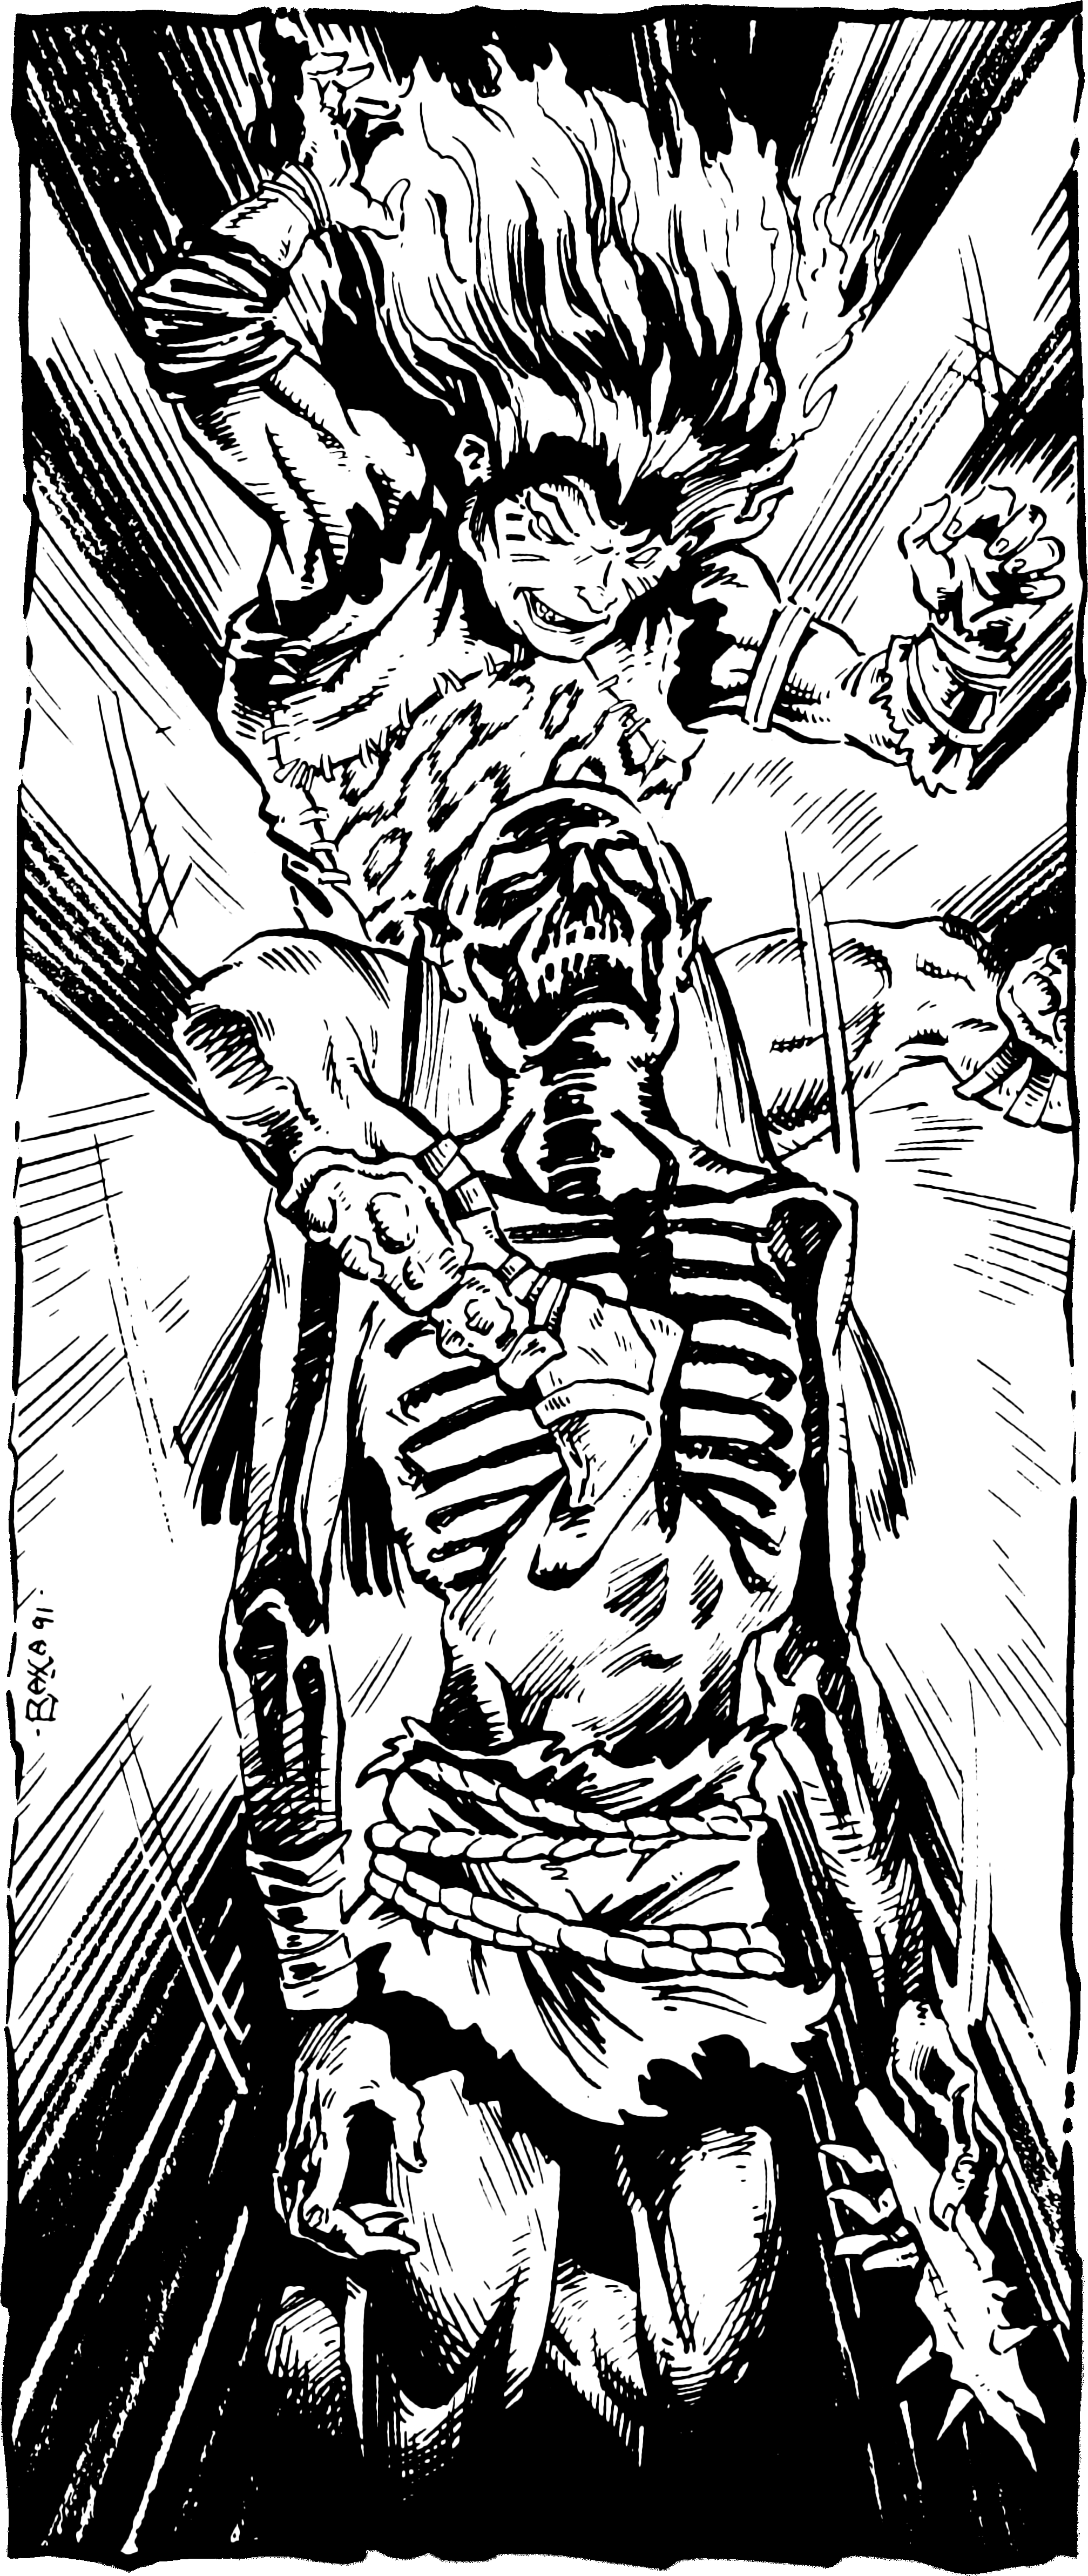
\includegraphics[width=\columnwidth]{images/psionic-1.png}
\par\textit{\small\textcopyright Wizards of the Coast, 2020.}
\end{figure}

\subsection{Making a Wilder}

Through experience, the wilder discovers supernatural powers that are an extension of his personality. Wilders know fewer powers than other manifesting classes, but their wild surge ability gives their powers greater flexibility. These surges are not without cost, however, and can have a great toll on the careless wilder.

\textbf{Races:} Psionic talent is common in the tablelands. Because of the limited access to psionic instruction, humans elves, halflings, and to a lesser extent, muls, are much more likely to be wilders than psions. Races that are less charismatic, less individualistic, and less prone to emotion, such as thri-kreen and dwarves rarely become wilders; more of them become psions or psychic warriors. The pterran culture glorifies the path of the psion, so wilders are rare. Half-giants tend to become wilders rather than psions, because even with psionic training, many half-giants lack the wit, Will, or focus to excel as psions.

\textbf{Alignment:} Though wilders have no inclinations towards good or evil, as a whole they tend to be chaotic.

\subsection{Game Rule Information}

\textbf{Hit Die:} d6.

\subsubsection{Class Skills}
\skill{Autohypnosis} (Wis), \skill{Balance} (Dex), \skill{Bluff} (Cha), \skill{Climb} (Str), \skill{Concentration} (Con), \skill{Craft} (Int), \skill{Escape Artist} (Dex), \skill{Intimidate} (Cha), \skill{Jump} (Str), \skill{Knowledge} (psionics) (Int), \skill{Listen} (Wis), \skill{Profession} (Wis), \skill{Psicraft} (Int), \skill{Sense Motive} (Wis), \skill{Spot} (Wis), \skill{Survival} (Wis), and \skill{Tumble} (Dex).

\textbf{Skill Points per Level:} 4 + Int modifier ($\times 4$ at 1st level).

\subsubsection{Class Features}

\textbf{Weapon and Armor Proficiency:} Wilders are proficient with all simple weapons, with light armor, and with shields (except tower shields).

\textbf{Power Points/Day:} A wilder's ability to manifest powers is limited by the power points she has available. Her base daily allotment of power points is given on \tabref{The Wilder}. In addition, she receives bonus power points per day if she has a high Charisma score (see \tabref{Ability Scores and Bonus Power Points}). Her race may also provide bonus power points per day, as may certain feats and items.

\textbf{Powers Known:} A wilder begins play knowing one wilder power of your choice. At every even-numbered class level after 1st, she unlocks the knowledge of new powers.

Choose the powers known from the wilder power list. (Exception: The feat \feat{Expanded Knowledge} do allow a wilder to learn powers from the lists of other classes.) A wilder can manifest any power that has a power point cost equal to or lower than her manifester level.

The total number of powers a wilder can manifest in a day is limited only by her daily power points.

A wilder simply knows her powers; they are ingrained in her mind. She does not need to prepare them (in the way that some spellcasters prepare their spells), though she must get a good night's sleep each day to regain all her spent power points.

The Difficulty Class for saving throws against wilder powers is 10 + the power's level + the wilder's Charisma modifier.

\textbf{Maximum Power Level Known:} A wilder begins play with the ability to learn 1st-level powers. As she attains higher levels, she may gain the ability to master more complex powers.

To learn or manifest a power, a wilder must have a Charisma score of at least 10 + the power's level.

\textbf{Wild Surge (Su):} A wilder can let her passion and emotion rise to the surface in a wild surge when she manifests a power. During a wild surge, a wilder gains phenomenal psionic strength, but may harm herself by the reckless use of her power (see Psychic Enervation, below).

A wilder can choose to invoke a wild surge whenever she manifests a power. When she does so, she gains +1 to her manifester level with that manifestation of the power. The manifester level boost gives her the ability to augment her powers to a higher degree than she otherwise could; however, she pays no extra power point for this wild surge. Instead, the additional 1 power point that would normally be required to augment the power is effectively supplied by the wild surge.

Level-dependent power effects are also improved, depending on the power a wilder manifests with her wild surge.

This improvement in manifester level does not grant her any other benefits (psicrystal abilities do not advance, she does not gain higher-level class abilities, and so on).

She cannot use the \feat{Overchannel} psionic feat and invoke her wild surge at the same time.

At 3rd level, a wilder can choose to boost her manifester level by two instead of one. At 7th level, she can boost her manifester level by up to three; at 11th level, by up to four; at 15th level, by up to five; and at 19th level, by up to six.

In all cases, the wild surge effectively pays the extra power point cost that is normally required to augment the power; only the unaugmented power point cost is subtracted from the wilder's power point reserve.

\textbf{Psychic Enervation (Ex):} Pushing oneself by invoking a wild surge is dangerous. Immediately following each wild surge, a wilder may be overcome by the strain of her effort. The chance of suffering psychic enervation is equal to 5\% per manifester level added with the wild surge.

A wilder who is overcome by psychic enervation is dazed until the end of her next turn and loses a number of power points equal to her wilder level.

\textbf{Elude Touch (Ex):} Starting at 2nd level, a wilder's intuition supersedes her intellect, alerting her to danger from touch attacks (including rays). She gains a bonus to Armor Class against all touch attacks equal to her Charisma bonus; however, her touch AC can never exceed her Armor Class against normal attacks.

\textbf{Surging Euphoria (Ex):} Starting at 4th level, when a wilder uses her wild surge ability, she gains a +1 morale bonus on attack rolls, damage rolls, and saving throws for a number of rounds equal to the intensity of her wild surge.

If a wilder is overcome by psychic enervation following her wild surge, she does not gain the morale bonus for this use of her wild surge ability.

At 12th level, the morale bonus on a wilder's attack rolls, damage rolls, and saving throws increases to +2. At 20th level, the bonus increases to +3.

\textbf{Volatile Mind (Ex):} A wilder's temperamental mind is hard to encompass with the discipline of telepathy. When any telepathy power is manifested on a wilder of 5th level or higher, the manifester of the power must pay 1 power point more than he otherwise would have spent.

The extra cost is not a natural part of that power's cost. It does not augment the power; it is simply a wasted power point. The wilder's volatile mind can force the manifester of the telepathy power to exceed the normal power point limit of 1 point per manifester level. If the extra cost raises the telepathy power's cost to more points than the manifester has remaining in his reserve, the power simply fails, and the manifester exhausts the rest of his power points.

At 9th level, the penalty assessed against telepathy powers manifested on a wilder is increased to 2 power points. At 13th level, the penalty increases to 3 power points, and at 17th level it increases to 4 power points.

As a standard action, a wilder can choose to lower this effect for 1 round.

\subsection{Playing a Wilder}
As a wilder, you adventure to practice your abilities and gain further understanding and mastery about the Will. You are very passionate about your powers, and you often push yourself to your limits with your wild surges, but you are not blind to its dangers.

\subsubsection{Religion}
Although wilders, like psions, draw their energies from within, wilder powers require less focus and discipline, so wilders are as likely as any other Athasian to be religious. A wilders religion can have a great impact on his power selection. A wilder who worships fire, for example, often discovers powers that involve light, heat or flame.

\subsubsection{Other Classes}
Wilder's opinions vary wildly. Some wilders view psions with awe, respecting the psion's greater knowledge and control; others chafe under the psion's perceived superiority complex.

\subsubsection{Combat}
In combat, you use your impressive array of psionic powers for both attack and defense against your enemies and opponents, just as any other psionicist would. Of course, as a wilder, you can call upon swells of psionic potential that other psionicists cannot access in the form of wild surges.

\subsubsection{Advancement}
Your interest on psionics is more than academic---it has been your motivating force for years. Perhaps you became a wilder after witnessing one destroying an entire village during one of his surges, or you vowed to gain control of the power you first displayed in your puberty every time you got were angered. Whatever the case, since the day you first became a wilder, you've worked to master a power more primal than spells and stronger than steel.

The powers you choose strongly shape your abilities. You are heavily invested in combat prowess as a result of the erratic and emotional nature of your power, but you have some flexibility in how you learn your powers. If you choose only offensive powers, you will have few defenses and limited versatility beyond combat, but you'll be devastating even in dire situations. If you focus on other powers, you will have more options outside a fight, but you might have only area attacks that could accidentally hurt a friend.

\vskip5cm
\subsection{Starting Packages}
\subsubsection{The Battle Wilder}
Mul Wilder

\textbf{Ability Scores:} Str 17, Dex 8, Con 16, Int 10, Wis 12, Cha 13.

\textbf{Skills:} \skill{Concentration}, \skill{Intimidate}, \skill{Psicraft}.

\textbf{Languages:} Common.

\textbf{Feat:} \feat{Combat Manifestation}.

\textbf{Weapons:} Longspear (1d8/$\times$3).

\textbf{Armor:} Scale mail (+4 AC).

\textbf{Other Gear:} Standard adventurer's kit, 20 cp.

\subsubsection{The Blaster}
Human Wilder

\textbf{Ability Scores:} Str 8, Dex 14, Con 13, Int 12, Wis 10, Cha 15.

\textbf{Skills:} \skill{Concentration}, \skill{Intimidate}, \skill{Knowledge} (psionics), \skill{Psicraft}.

\textbf{Languages:} Common.

\textbf{Feat:} \feat{Lightning Reflexes}, \feat{Psionic Endowment}.

\textbf{Weapons:} Spear (1d8/$\times$3, 6 m)

Light crossbow with 20 bolts (1d8/19--20, 24 m).

\textbf{Armor:} Leather (+2 AC).

\textbf{Other Gear:} Standard adventurer's kit, 26 cp.

\subsubsection{The Sharpshooter}
Halfling Wilder

\textbf{Ability Scores:} Str 6, Dex 16, Con 13, Int 12, Wis 10, Cha 15.

\textbf{Skills:} \skill{Concentration}, \skill{Intimidate}, \skill{Spot} (cc).

\textbf{Languages:} Halfling.

\textbf{Feat:} \feat{Point Blank Shot}.

\textbf{Weapons:} Spear (1d8/$\times$3, 6 m)

Light crossbow with 20 bolts (1d8/19--20, 24 m).

\textbf{Armor:} Leather (+2 AC).

\textbf{Other Gear:} Standard adventurer's kit, 26 cp.

\subsection{Wilders on Athas}
\Quote{Something seemed strange the second I saw Nakua's face. It's odd. He acted like a different person. My friend Kuko asked him if he was really Nakua or if he was someone else. And those were his last words}{Ekee, elven dancer}

Psionic is very common on Athas, and wilders can be widely found in the Tablelands, representing psionic energy in its most raw state, and change for change's sake. Neutral wilders are rare, but such characters become famous within the ranks of their comrades, since their vision is unclouded by moral concerns.

Wilders know that using psionic powers can be strenuous, and the limit of a character's endurance is his Will. Eventually, even the most powerful of masters becomes exhausted and must rest to replenish his strength. When wounds and exhaustion cloud the vision and the mind swims in delirium, only the greatest wilders possess the Will to continue using their powers.

\subsubsection{Daily Life}

Wilders spend their days in travel and contemplation, with an occasional rant and wild outburst (usually against the foes an adventurer comes across). They enjoy talking about their psionic abilities and about their life philosophies.

\subsubsection{Notables}

The xenophobic Kenkus (FFN 126) are the race to most commonly sport wilders, although no one knows for sure why. Elves, due to their chaotic nature, also seem to have a higher rate of wilders in their milieu.

\subsubsection{Organizations}

A wilder's path is his own to thread, since no overarching organization exists to recruit you into its ranks. Most wilders are just too erratic and freedom-loving to join one, anyway.

\subsubsection{NPC Reactions}

Most people do not understand the difference between a psion and a wilder, so their attitudes span the spectrum. Psions NPC attitudes range from indifferent to unfriendly, although most psiologists (page 104) tend to have their attitude bent towards hostile.

\subsubsection{Wilder Lore}

Characters with ranks in \skill{Knowledge} (psionics) can research wilders to learn more about them. When a character makes a skill check, read or paraphrase the following, including the information from lower DCs.

\textbf{DC 10:} A wilder is a kind of psionicist that can trigger a surge of psionic power beyond control.

\textbf{DC 15:} Wilders usually become very weak, both physically and mentally, after unleashing their psionic surges.

\textbf{DC 20:} Experienced wilders learn how to further tap into their Will and manage to also strengthen their bodies while surging.
\Class{Wizard}
{So what if the land becomes barren? It's not like we're going to stick around.}{Datuu Dawnchaser, elf defiler}

Athasian wizards drain energy from the surrounding soil. The method used labels the wizard as a defiler or a preserver. Preservers have the self-control to gather energy without destroying plants. Those who do not, or who feel no remorse about the damage caused, become Defilers. Defilers leave behind sterile soil and infertile ash when they cast spells. Because of this, most wastelanders blame wizards for the desert landscape that dominates the Tablelands today, and their hatred extends to defilers and preservers alike. In the seven cities, arcane magic is outlawed and feared.

Writing is also illegal in the Tablelands, thus wizards have to go to great lengths to conceal their spellbooks, and they have refined this art to the point where even fellow wizards can be hard pressed to identify a spell book. When found, they are precious resources, hoarded and studied by wizards thirsty for knowledge or power.

\SpellcasterTable{The Wizard}{.3cm}{
1st & +0 & +0 & +0 & +2 & Path, summon familiar, \feat{Scribe Scroll} & 3 & 1 &&&&&&&&\\
2nd & +1 & +0 & +0 & +3 &  & 4 & 2 &&&&&&&&\\
3rd & +1 & +1 & +1 & +3 &  & 4 & 2 & 1 &&&&&&&\\
4th & +2 & +1 & +1 & +4 &  & 4 & 3 & 2 &&&&&&&\\
5th & +2 & +1 & +1 & +4 & Bonus feat & 4 & 3 & 2 & 1 &&&&&&\\
6th & +3 & +2 & +2 & +5 &  & 4 & 3 & 3 & 2 &&&&&&\\
7th & +3 & +2 & +2 & +5 &  & 4 & 4 & 3 & 2 & 1 &&&&&\\
8th & +4 & +2 & +2 & +6 &  & 4 & 4 & 3 & 3 & 2 &&&&&\\
9th & +4 & +3 & +3 & +6 &  & 4 & 4 & 4 & 3 & 2 & 1 &&&&\\
10th & +5 & +3 & +3 & +7 & Bonus feat & 4 & 4 & 4 & 3 & 3 & 2 &&&&\\
11th & +5 & +3 & +3 & +7 &  & 4 & 4 & 4 & 4 & 3 & 2 & 1 &&&\\
12th & +6/+1 & +4 & +4 & +8 &  & 4 & 4 & 4 & 4 & 3 & 3 & 2 &&&\\
13th & +6/+1 & +4 & +4 & +8 &  & 4 & 4 & 4 & 4 & 4 & 3 & 2 & 1 &&\\
14th & +7/+2 & +4 & +4 & +9 &  & 4 & 4 & 4 & 4 & 4 & 3 & 3 & 2 &&\\
15th & +7/+2 & +5 & +5 & +9 & Bonus feat & 4 & 4 & 4 & 4 & 4 & 4 & 3 & 2 & 1 &\\
16th & +8/+3 & +5 & +5 & +10 &  & 4 & 4 & 4 & 4 & 4 & 4 & 3 & 3 & 2 &\\
17th & +8/+3 & +5 & +5 & +10 &  & 4 & 4 & 4 & 4 & 4 & 4 & 4 & 3 & 2 & 1\\
18th & +9/+4 & +6 & +6 & +11 &  & 4 & 4 & 4 & 4 & 4 & 4 & 4 & 3 & 3 & 2\\
19th & +9/+4 & +6 & +6 & +11 &  & 4 & 4 & 4 & 4 & 4 & 4 & 4 & 4 & 3 & 3\\
20th & +10/+5 & +6 & +6 & +12 & Bonus feat & 4 & 4 & 4 & 4 & 4 & 4 & 4 & 4 & 4 & 4
}

\subsection{Making a Wizard}
The wizard's greatest strength is also his greatest liability. Often wizards will conceal their abilities, learning to mask their spellcasting behind other actions. For all but the most powerful wizards, secrecy is of prime importance, and some will not exercise their power in the presence of those that they do not feel they can trust. Because of this, and because of their generally frail nature, wizards can often be seen as a liability by those not aware of the power they hide.

\textbf{Races:} Elves and humans are the most likely to be wizards. Elves are more tolerant of the faults of magic, even at its worst, due to their nomadic nature. Defiling simply isn't as much of a concern if the ruined land is fifty miles behind you by the end of the next day. The solitary life lead by most half-elves makes it easier for them to conceal their wizardry, should they choose to follow that path. Some rare halflings and pterrans will take up the arts of wizardry, but these races are so closely tuned to flow of life on Athas that they will never willingly defile. Half-giants, trusting and slow-witted, rarely become wizards, and those that do rarely survive for long. Dwarves rarely take to the magic arts, though their focus allows those that do to become exceptionally skilled. Thri-kreen and muls almost never become wizards.

\textbf{Alignment:} Overall, most wizards display a tendency towards lawfulness. The self-control and restraint necessary to keep oneself secret, as well as the disciplined need for long days of studying take their toll on many of the less careful wizards. Most wizards of good alignment have developed the skill and control necessary to master preserving, and only in the direst of situations would a good-aligned wizard defile. Neutral or evil wizards, however, are more likely to become defilers, though evil preservers are not unheard of.

\subsection{Game Rule Information}

\textbf{Alignment:} Preservers can be of any alignment. Defilers must be of any nongood.

\textbf{Hit Die:} d4.

\subsubsection{Class Skills}
\skill{Bluff} (Cha), \skill{Concentration} (Con), \skill{Craft} (Int), \skill{Decipher Script} (Int), \skill{Disguise} (Cha), \skill{Knowledge} (all skills, taken individually) (Int), \skill{Literacy} (N/A), \skill{Profession} (Wis), and \skill{Spellcraft} (Int).

\textbf{Skill Points per Level:} 2 + Int modifier ($\times4$ at 1st level).

\subsubsection{Class Features}
\textbf{Weapon and Armor Proficiency:} Wizards are proficient with the club, dagger, heavy crossbow, light crossbow, and quarterstaff, but not with any type of armor or shield. Armor of any type interferes with a wizard's movements, which can cause her spells with somatic components to fail.

\textbf{Spells:} A wizard casts arcane spells which are drawn from the wizard spell list. A wizard must choose and prepare her spells ahead of time (see below).

To learn, prepare, or cast a spell, the wizard must have an Intelligence score equal to at least 10 + the spell level. The Difficulty Class for a saving throw against a wizard's spell is 10 + the spell level + the wizard's Intelligence modifier.

Like other spellcasters, a wizard can cast only a certain number of spells of each spell level per day. Her base daily spell allotment is given on \tabref{The Wizard}. In addition, she receives bonus spells per day if she has a high Intelligence score.

A wizard may know any number of spells. She must choose and prepare her spells ahead of time by getting a good night's sleep and spending 1 hour studying her spellbook. While studying, the wizard decides which spells to prepare.

\begin{figure*}[b!]
\centering
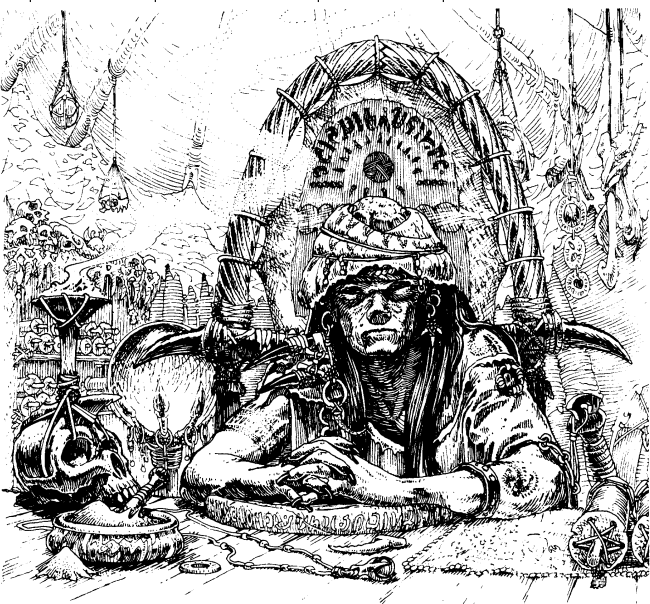
\includegraphics[width=\textwidth-2cm]{images/wizard-5.png}
\WOTC
\end{figure*}

\textbf{Bonus Languages:} A wizard may substitute Draconic for one of the bonus languages available to the character because of her race.

\textbf{Familiar:} A wizard can obtain a familiar. Doing so takes 24 hours and uses up magical materials that cost 100 ceramic pieces. A familiar is a magical beast that resembles a small animal and is unusually tough and intelligent. The creature serves as a companion and servant.

The wizard chooses the kind of familiar he gets. As the wizard advances in level, his familiar also increases in power.

If the familiar dies or is dismissed by the wizard, the wizard must attempt a DC 15 Fortitude saving throw. Failure means he loses 200 experience points per wizard level; success reduces the loss to one-half that amount. However, a wizard's experience point total can never go below 0 as the result of a familiar's demise or dismissal. A slain or dismissed familiar cannot be replaced for a year and day. A slain familiar can be raised from the dead just as a character can be, and it does not lose a level or a Constitution point when this happy event occurs.

A character with more than one class that grants a familiar may have only one familiar at a time.

\textbf{Scribe Scroll:} At 1st level, a wizard gains \feat{Scribe Scroll} as a bonus feat.

\textbf{Path:} At 1st level, a wizard must choose a philosophical path: preservation or defilement. This choice is not final. Preservers can defile and be corrupted, and defilers can get redemption.

\textit{Path Dexter:} Wizards who take this path are preservers. They master the balance of the arcane, casting spells with no collateral environmental damage.

Preservers learn one spell at each wizard level from abjuration or divination schools. They are drawn to protection and information spells.

\textit{Path Sinister:} This path is allowed only for nongood wizards. The wizards who take this path are defilers. With every spell cast, defilers take the life out of the plants and soil around them.

Defilers learn one spell at each wizard level from evocation or necromancy schools. They best utilize those darker and more destructive schools.

\textbf{Bonus Feats:} At 5th, 10th, 15th, and 20th level, a wizard gains a bonus feat. At each such opportunity, she can choose a metamagic feat, a raze feat, an item creation feat, or \feat{Spell Mastery}. The wizard must still meet all prerequisites for a bonus feat, including caster level minimums.

These bonus feats are in addition to the feat that a character of any class gets from advancing levels. The wizard is not limited to the categories of item creation feats, metamagic feats, or Spell Mastery when choosing these feats.

\textbf{Spellbooks:} A wizard must study her spellbook each day to prepare her spells. She cannot prepare any spell not recorded in her spellbook, except for read magic, which all wizards can prepare from memory.

A wizard begins play with a spellbook containing all 0-level wizard spells (except those from her prohibited school or schools, if any; see School Specialization, below) plus three 1st-level spells of your choice. For each point of Intelligence bonus the wizard has, the spellbook holds one additional 1st-level spell of your choice.

At each new wizard level, she gains three new spells of any spell level or levels that she can cast (based on her new wizard level) for her spellbook, one of which must be from her path's schools. At any time, a wizard can also add spells found in other wizards' spellbooks to her own.

\subsubsection{Familiars}
A familiar is a normal animal that gains new powers and becomes a magical beast when summoned to service by a wizard. It retains the appearance, Hit Dice, base attack bonus, base save bonuses, skills, and feats of the normal animal it once was, but it is treated as a magical beast instead of an animal for the purpose of any effect that depends on its type. Only a normal, unmodified animal may become a familiar. An animal companion cannot also function as a familiar.

A familiar also grants special abilities to its master, as given on the table below. These special abilities apply only when the master and familiar are within 1.5 kilometer of each other.

Levels of different classes that are entitled to familiars stack for the purpose of determining any familiar abilities that depend on the master's level.

\Table{Familiars}{l X}{
	\tableheader Familiar & \tableheader Special\\
	Bat & Master gains a +3 bonus on \skill{Listen} checks\\
	Cat & Master gains a +3 bonus on \skill{Move Silently} checks\\
	Dustgull & Master gains a +3 bonus on \skill{Spot} checks\\
	Hawk & Master gains a +3 bonus on \skill{Spot} checks in bright light\\
	Kes'trekel & Master gains a +2 bonus on Reflex saves\\
	Lizard & Master gains a +3 bonus on \skill{Climb} checks\\
	Owl & Master gains a +3 bonus on \skill{Spot} checks in shadows\\
	Rat & Master gains a +2 bonus on Fortitude saves\\
	Raven$\dagger$ & Master gains a +3 bonus on \skill{Appraise} checks\\
	Skyfish & Master gains a +3 bonus on \skill{Swim} checks\\
	Sygra & Master gains a +3 hit points\\
	Tiny viper & Master gains a +3 bonus on \skill{Bluff} checks\\
	% Toad & Master gains +3 hit points\\
	% Weasel & Master gains a +2 bonus on Reflex saves
	\rowcolor{white}
	\multicolumn{2}{p{\columnwidth}}{$\dagger$ A raven familiar can speak one language of its master's choice as a supernatural ability.}
}


\textbf{Familiar Basics:} Use the basic statistics for a creature of the familiar's kind, but make the following changes:

\textit{Hit Dice:} For the purpose of effects related to number of Hit Dice, use the master's character level or the familiar's normal HD total, whichever is higher.

\textit{Hit Points:} The familiar has one-half the master's total hit points (not including temporary hit points), rounded down, regardless of its actual Hit Dice.

\textit{Attacks:} Use the master's base attack bonus, as calculated from all his classes. Use the familiar's Dexterity or Strength modifier, whichever is greater, to get the familiar's melee attack bonus with natural weapons.

Damage equals that of a normal creature of the familiar's kind.

\textit{Saving Throws:} For each saving throw, use either the familiar's base save bonus (Fortitude +2, Reflex +2, Will +0) or the master's (as calculated from all his classes), whichever is better. The familiar uses its own ability modifiers to saves, and it doesn't share any of the other bonuses that the master might have on saves.

\textit{Skills:} For each skill in which either the master or the familiar has ranks, use either the normal skill ranks for an animal of that type or the master's skill ranks, whichever are better. In either case, the familiar uses its own ability modifiers. Regardless of a familiar's total skill modifiers, some skills may remain beyond the familiar's ability to use.

\Table{Familiar Progression}{b{1.4cm} Z{1.2cm} c X}{
	\tableheader Master Class Level & \tableheader Natural Armor Adj. & \tableheader Int & \tableheader Special\\
	1st--2nd & +1 & 6 & Alertness, improved evasion, share spells, empathic link\\
	3rd--4th & +2 & 7 & Deliver touch spells\\
	5th--6th & +3 & 8 & Speak with master\\
	7th--8th & +4 & 9 & Speak with animals of its kind\\
	9th--10th & +5 & 10 & \\
	11th--12th & +6 & 11 & Spell resistance\\
	13th--14th & +7 & 12 & Scry on familiar\\
	15th--16th & +8 & 13 & \\
	17th--18th & +9 & 14 & \\
	19th--20th & +10 & 15 &
}

\textbf{Familiar Ability Descriptions:} All familiars have special abilities (or impart abilities to their masters) depending on the master's combined level in classes that grant familiars, as shown on the table above. The abilities given on the table are cumulative.

\textit{Natural Armor Adj.:} The number noted here is an improvement to the familiar's existing natural armor bonus.

\textit{Int:} The familiar's Intelligence score.

\textit{Alertness (Ex):} While a familiar is within arm's reach, the master gains the Alertness feat.

\textit{Improved Evasion (Ex):} When subjected to an attack that normally allows a Reflex saving throw for half damage, a familiar takes no damage if it makes a successful saving throw and half damage even if the saving throw fails.

\textit{Share Spells:} At the master's option, he may have any spell (but not any spell-like ability) he casts on himself also affect his familiar. The familiar must be within 1.5 meter at the time of casting to receive the benefit.

If the spell or effect has a duration other than instantaneous, it stops affecting the familiar if it moves farther than 1.5 meter away and will not affect the familiar again even if it returns to the master before the duration expires. Additionally, the master may cast a spell with a target of ``You'' on his familiar (as a touch range spell) instead of on himself.

A master and his familiar can share spells even if the spells normally do not affect creatures of the familiar's type (magical beast).

\textit{Empathic Link (Su):} The master has an empathic link with his familiar out to a distance of up to 1.5 kilometer. The master cannot see through the familiar's eyes, but they can communicate empathically. Because of the limited nature of the link, only general emotional content can be communicated.

Because of this empathic link, the master has the same connection to an item or place that his familiar does.

\textit{Deliver Touch Spells (Su):} If the master is 3rd level or higher, a familiar can deliver touch spells for him. If the master and the familiar are in contact at the time the master casts a touch spell, he can designate his familiar as the ``toucher.'' The familiar can then deliver the touch spell just as the master could. As usual, if the master casts another spell before the touch is delivered, the touch spell dissipates.

\textit{Speak with Master (Ex):} If the master is 5th level or higher, a familiar and the master can communicate verbally as if they were using a common language. Other creatures do not understand the communication without magical help.

\textit{Speak with Animals of Its Kind (Ex):} If the master is 7th level or higher, a familiar can communicate with animals of approximately the same kind as itself (including dire varieties): bats with bats, rats with rodents, cats with felines, hawks and owls and ravens with birds, lizards and snakes with reptiles, toads with amphibians, weasels with similar creatures (weasels, minks, polecats, ermines, skunks, wolverines, and badgers). Such communication is limited by the intelligence of the conversing creatures.

\textit{Spell Resistance (Ex):} If the master is 11th level or higher, a familiar gains spell resistance equal to the master's level + 5. To affect the familiar with a spell, another spellcaster must get a result on a caster level check (1d20 + caster level) that equals or exceeds the familiar's spell resistance.

\textit{Scry on Familiar (Sp):} If the master is 13th level or higher, he may scry on his familiar (as if casting the scrying spell) once per day.

\subsubsection{School Specialization}
A school is one of eight groupings of spells, each defined by a common theme. If desired, a wizard may specialize in one school of magic (see below). Specialization allows a wizard to cast extra spells from her chosen school, but she then never learns to cast spells from some other schools.

A specialist wizard can prepare one additional spell of her specialty school per spell level each day. She also gains a +2 bonus on \skill{Spellcraft} checks to learn the spells of her chosen school.

The wizard must choose whether to specialize and, if she does so, choose her specialty at 1st level. At this time, she must also give up two other schools of magic (unless she chooses to specialize in divination; see below), which become her prohibited schools.

A wizard can never give up divination to fulfill this requirement.

Spells of the prohibited school or schools are not available to the wizard, and she can't even cast such spells from scrolls or fire them from wands. She may not change either her specialization or her prohibited schools later.

The eight schools of arcane magic are abjuration, conjuration, divination, enchantment, evocation, illusion, necromancy, and transmutation.

Spells that do not fall into any of these schools are called universal spells.

\begin{figure}[t!]
\centering
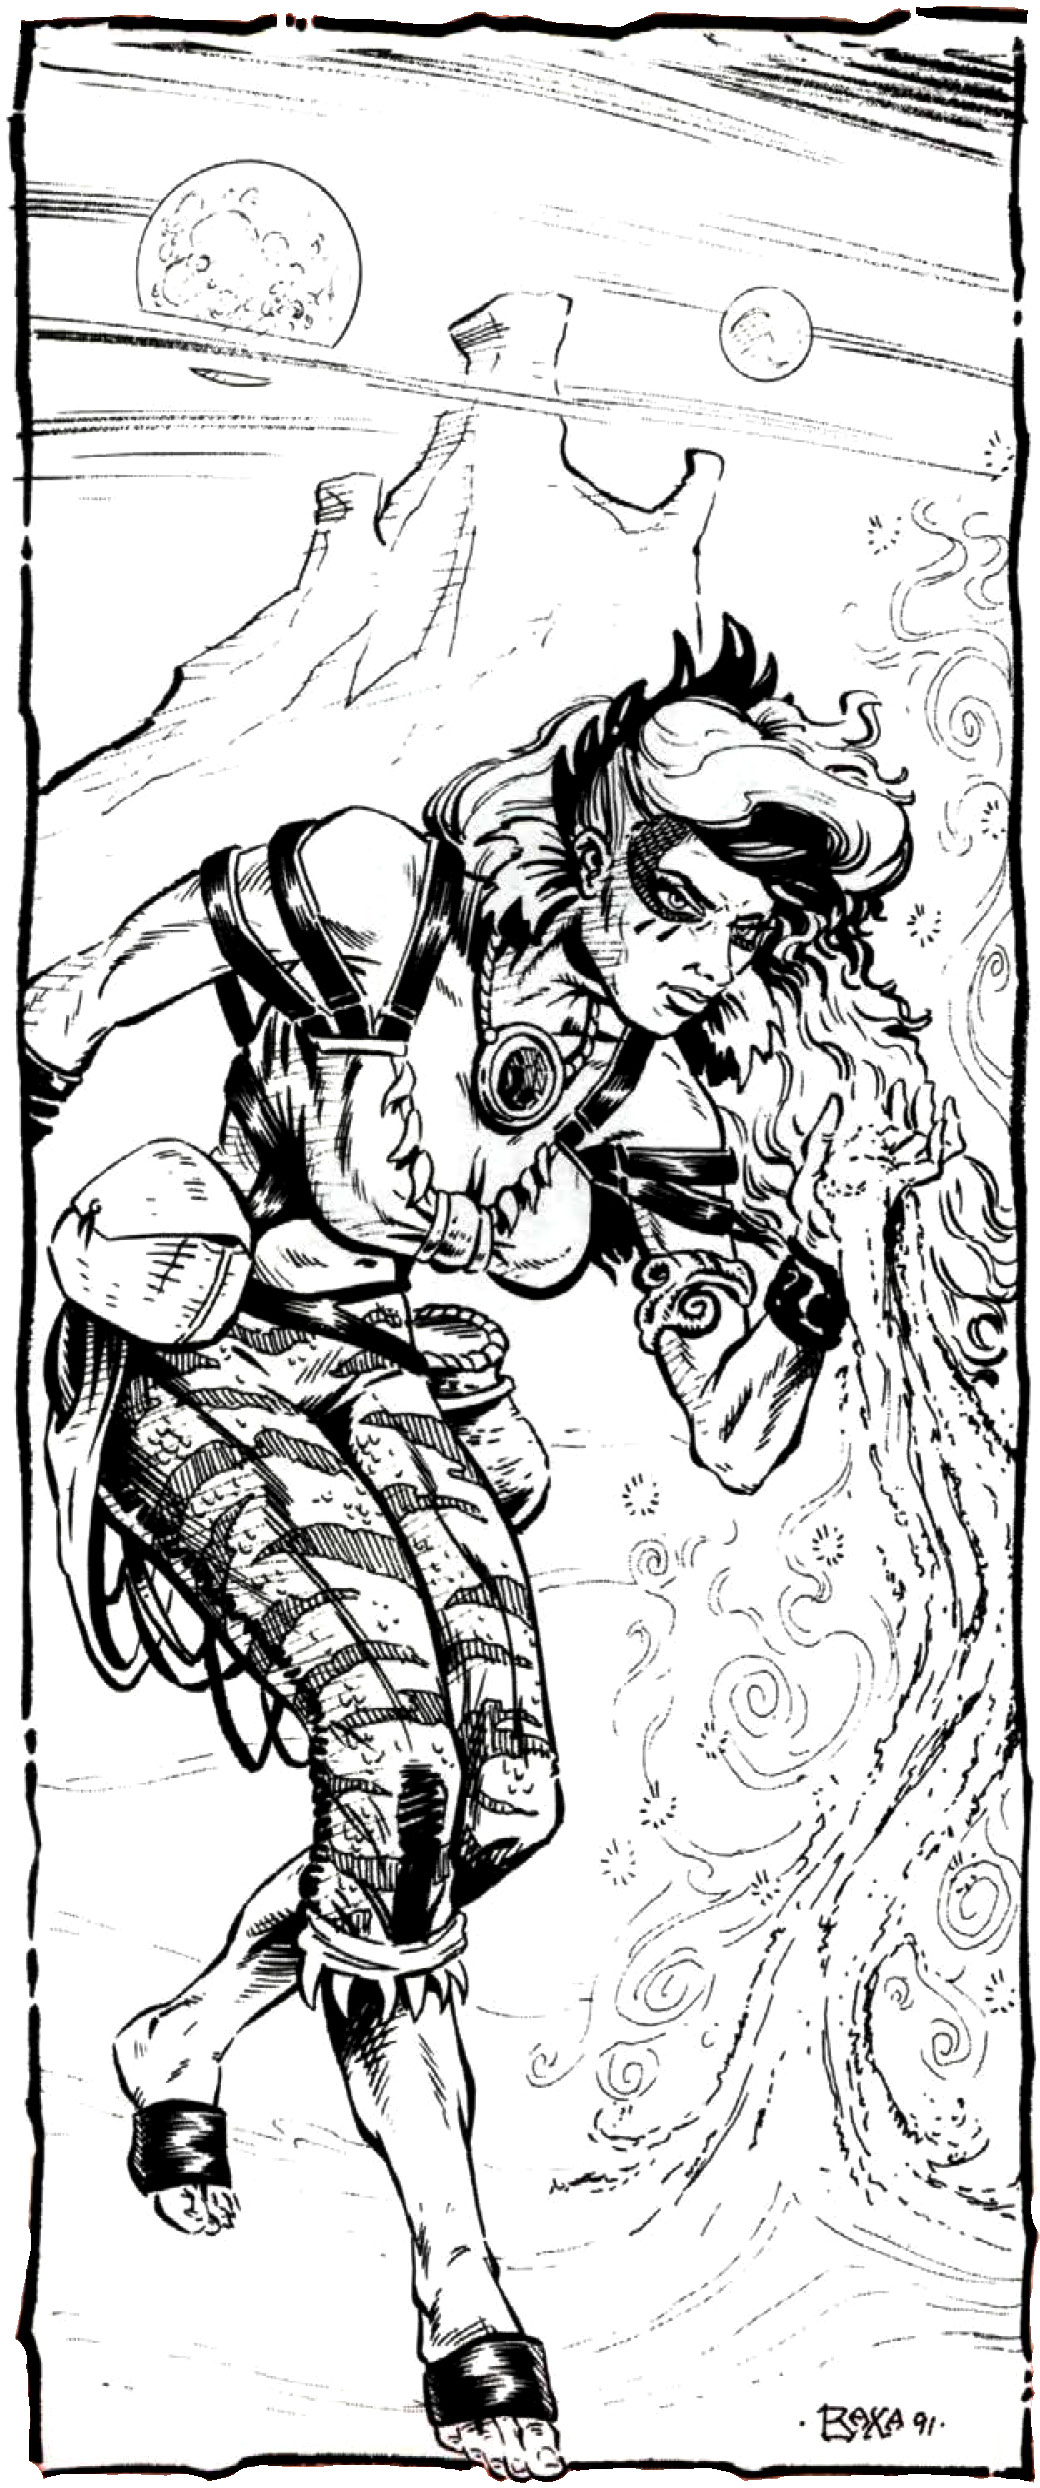
\includegraphics[width=\columnwidth]{images/wizard-2.png}
\WOTC
\end{figure}


\textbf{Abjuration:} Spells that protect, block, or banish. An abjuration specialist is called an abjurer.

\textbf{Conjuration:} Spells that bring creatures or materials to the caster. A conjuration specialist is called a conjurer.

\textbf{Divination:} Spells that reveal information. A divination specialist is called a diviner. Unlike the other specialists, a diviner must give up only one other school.

\textbf{Enchantment:} Spells that imbue the recipient with some property or grant the caster power over another being. An enchantment specialist is called an enchanter.

\textbf{Evocation:} Spells that manipulate energy or create something from nothing. An evocation specialist is called an evoker.

\textbf{Illusion:} Spells that alter perception or create false images. An illusion specialist is called an illusionist.

\textbf{Necromancy:} Spells that manipulate, create, or destroy life or life force. A necromancy specialist is called a necromancer.

\textbf{Transmutation:} Spells that transform the recipient physically or change its properties in a more subtle way. A transmutation specialist is called a transmuter.

\textbf{Universal:} Not a school, but a category for spells that all wizards can learn. A wizard cannot select universal as a specialty school or as a prohibited school. Only a limited number of spells fall into this category.

\subsubsection{Ex-Defilers}
Arcane casters who defile must roll a Will save DC 10 + spell level + amount of times previously defiled. Failing this save, they become defilers. Preservers succeeding the save lose their preserver status and become tainted. For more rules on defiling, see \chapref{Magic}.

Tainted wizards are not defilers, but risk becoming so. Tainted wizards may seek redemption from a druid. The druid, if willing and able, can cast a \spell{conversion} spell on the tainted wizard, restoring her preserver status (reset the number of times defiled to zero). The wizard loses 100 XP per arcane spellcaster level.

Defilers can also seek redemption, but lose 1,000 XP per arcane spellcaster level. Usually the defiler must undertake a quest or otherwise demonstrate a true willingness to redeem herself before the druid casts the \spell{conversion} spell.


\subsection{Playing a Wizard}
You are a master of arcane secrets. You have learned, either on your own, or from someone in your family, how to draw on vegetable life in order to power your spells. But such power comes with a caveat, arcane magic is universally feared and hated. You might be inclined to see conspiracies and enemies where none exist, so accustomed are you to being hunted and persecuted by the general populace and sorcerer-king's templars because of your talents.

Mostly, you adventure to perfect your understanding and mastery of magic. You likely prefer endeavors that allow frequent use of your abilities, or those that promise access to ancient lore. You might have personal goals as well, and it's not uncommon for an Athasian wizard to adventure for the sake of riches, power, eternal life, or any other ``standard'' adventurer motive.

\subsubsection{Religion}
Wizards frequently find themselves at odds with the elemental forces that grant clerics their powers, though it is not unheard of for preservers to forge an Elemental Pact. Some preservers might also associate themselves with the assorted Spirits of the Land. Since they understand the sorcerer-kings to simply be exceptionally advanced wizards, they are not given to revering their kings, as some of their more naive brothers are known to do.

\subsubsection{Other Classes}
Wizards have a difficult time relating to most of the other classes. Templars and wizards are, in most cases, deadly enemies across an irreconcilable gap---the exception is those rare defilers in the employ of the sorcerer-kings. Likewise, druids are likely to consider any wizard a potential defiler, and would turn on a companion the moment this suspicion is confirmed. Due to their similar, ``underground'' nature, wizards feel a certain respect for bards. While preservers enjoy an uneasy truce with the elemental powers, defilers and paraelemental clerics tend get along quite well.

\subsubsection{Combat}
Athasian wizards stay back from melee and use your spells to either destroy your enemies or enhance your companion's abilities. Secrecy is a major component, even more so if you are a defiler. Casting even of the simplest of arcane spells can focus all of your enemies' attention to you, even more so if you are a defiler. Be prepared to run of fly away in such cases.

\subsubsection{Advancement}
Continuing your advancement as a wizard requires a substantial amount of time and effort. You must procure and study arcane texts, not merely to learn new spells, but to comprehend the nature of what you do.

When you not studying, you are practicing, training your mind and your body to channel ever greater amounts of life force.

As you start to progress in the class, consider studying other sources of arcane energy, such as the Black, the Gray, and the Cerulean, since those would remove your dependency on vegetable life around you. Most wizards seek to become some day as powerful as Dragon Kings or the fabled winged creature the Urikite known as Korgunard turned into.

Mechanically, you should increase your Intelligence and Charisma as you attain levels. Beyond this, focus on feats (such as Path Dexter or Path Sinister) and skills that enhance your spells and provide you the abilities you need to remain in secrecy, mainly Bluff and Disguise.

\vskip3cm

\subsection{Starting Packages}
\subsubsection{The Dexter}
Pterran Wizard

\textbf{Ability Scores:} Str 8, Dex 10, Con 10, Int 15, Wis 16, Cha 15.

\textbf{Skills:} \skill{Bluff}, \skill{Concentration}, \skill{Disguise}, \skill{Knowledge} (arcana), \skill{Knowledge} (local), \skill{Spellcraft}.

\textbf{Languages:} Common, Elven, Saurian.

\textbf{Feat:} \feat{Path Dexter}.

\textbf{Weapons:} Dagger (1d4/19--20, 3 m)

Light crossbow with 20 bolts (1d6/$\times$3, 18 m).

\textbf{Armor:} Padded (+1 AC).

\textbf{Other Gear:} Standard adventurer's kit, spell

component pouch, 31 cp.

\subsubsection{The Concurrent}
Human Wizard

\textbf{Ability Scores:} Str 8, Dex 13, Con 10, Int 15, Wis 14, Cha 12.

\textbf{Skills:} \skill{Bluff}, \skill{Concentration}, \skill{Decipher Script}, \skill{Disguise}, \skill{Knowledge} (arcana), \skill{Knowledge} (local), \skill{Spellcraft}.

\textbf{Languages:} City language, Common, Elven.

\textbf{Feat:} \feat{Alertness}, \feat{Improved Initiative}.

\textbf{Weapons:} Dagger (1d4/19--20, 3 m)

Light crossbow with 20 bolts (1d6/$\times$3, 18 m).

\textbf{Armor:} Padded (+1 AC).

\textbf{Other Gear:} Standard adventurer's kit, spell component pouch, 31 cp.

\subsubsection{The Sinister}
Elf Wizard

\textbf{Ability Scores:} Str 10, Dex 16, Con 10, Int 15, Wis 13, Cha 8.

\textbf{Skills:} \skill{Bluff}, \skill{Concentration}, \skill{Knowledge} (arcana), \skill{Knowledge} (local), \skill{Spellcraft}.

\textbf{Languages:} City language, Common, Elven.

\textbf{Feat:} \feat{Destructive Raze}.

\textbf{Weapons:} Dagger (1d4/19--20, 3 m)

Light crossbow with 20 bolts (1d6/$\times$3, 18 m).

\textbf{Armor:} Padded (+1 AC).

\textbf{Other Gear:} Standard adventurer's kit, spell component pouch, 31 cp.

\subsection{Wizards on Athas}
\Quote{'Witch!' they chanted. 'Kill the witch!' By the time the soldiers woke, the crowd had finished her off, and worse. The mage's death did not satisfy the mob; her body suffered much more. When the mul leader shouted, 'we'll take her and burn her!' they cheered. For the only time in my life I saw a crowd cheer for Kalak's guards. For the first time I saw wizard's magic. For the first time I understood its peril.}{Manok, Tyrian wizard}

On Athas, the energy for wizardly magic doesn't come from some extradimensional source as it does on other worlds, but from the living environment itself. It provides great power to those who can gather and shape it, though the cost to Athas can be beyond measure.

In recent times wizards have emerged who have learned to draw energy from alternate sources that have no impact on the environment, see Prestige Class Appendix I for more information.

\subsubsection{Daily Life}
The kinds of activities that appeal to wizards depend largely on their alignment and energy gathering method. Good wizards spend their time trying to restore the devastation of Athas and fighting against the forces of the sorcerer-kings, while evil preservers of defilers are interested in helping themselves.

When not adventuring, Athasian wizards spend the majority of their time in study and in hiding. Much like wizards from other settings, they must constantly research new spells and study ancient arcane texts so thoroughly that they have little time to devote to other endeavors.

\subsubsection{Notables}
Usually wizards try to stay incognito for as long as they can, since their survival depends on it. However, a few wizards manage to become quite famous on Athas. Royal defilers and arena necromancers, such as Dote Mal Payn, even though hated by the general populace are sponsored by their sorcerer-kings and do not need to hide their skills. Sadira of Tyr was made famous for her contribution in killing King Kalak the Tyrant and the Dragon, and she has become the first (and maybe the only one) wizard able to tap into the power of the crimson sun. The most famous wizards are the Dragon Kings, of course, who can destroy both plant life and living creatures to power their spells.

\subsubsection{Organizations}
Wizardly magic on Athas isn't as codified and formal as it is in other campaign settings. For example, there are no academies or colleges for teaching the wizardly arts. Instead, a wizard-in-training must find a teacher, which isn't very easy in a world where wizards must hide their profession in order to survive. For protection from nearly universal hatred, the good wizards of Athas and their allies have formed secret societies, collectively known as the Veiled Alliance.

However, each city-state holds a different Alliance, they do not cooperate, and they share no leaders. Members of one Alliance do not automatically become members of another. At best, the different groups respect each other, and may offer courtesy assistance to a foreign member who arrives in town.

Defilers don't usually organize together, but they often join organizations, especially Merchant Houses and raiding tribes.

\subsubsection{NPC Reactions}
Arcane magic in Athas is viewed as more dangerous and destructive than helpful, so general NPC attitudes towards someone suspected to be a wizard range from indifferent to unfriendly. If a NPC actually witness a wizard drawing magical energy or casting a spell, the resultant fear and hatred shifts the NPC's attitude toward hostile.

Arcane magic is banned in almost all city-states; Tyr has unbanned it after FY 0 after Kalak was killed and Kurn has no qualms about preserving magic. Templars constantly patrol the streets searching for wizards and arcane items.

\subsubsection{Wizard Lore}

Characters with ranks in \skill{Knowledge} (arcana) can research wizards to learn more about them. When a character makes a skill check, read or paraphrase the following, including the information from lower DCs.

\textbf{DC 10:} Wizards are magic users that fuel their spells with plant life.

\textbf{DC 15:} A wizard can be either a defiler or a preserver. Only the first destroys the land when casting a spell. Defilers can increase the potency of their spells by destructing larger areas of vegetation than necessary.

\textbf{DC 20:} Some say that other wizards have developed a way to draw energy from other source than plants.


\begin{figure}[b!]
\centering
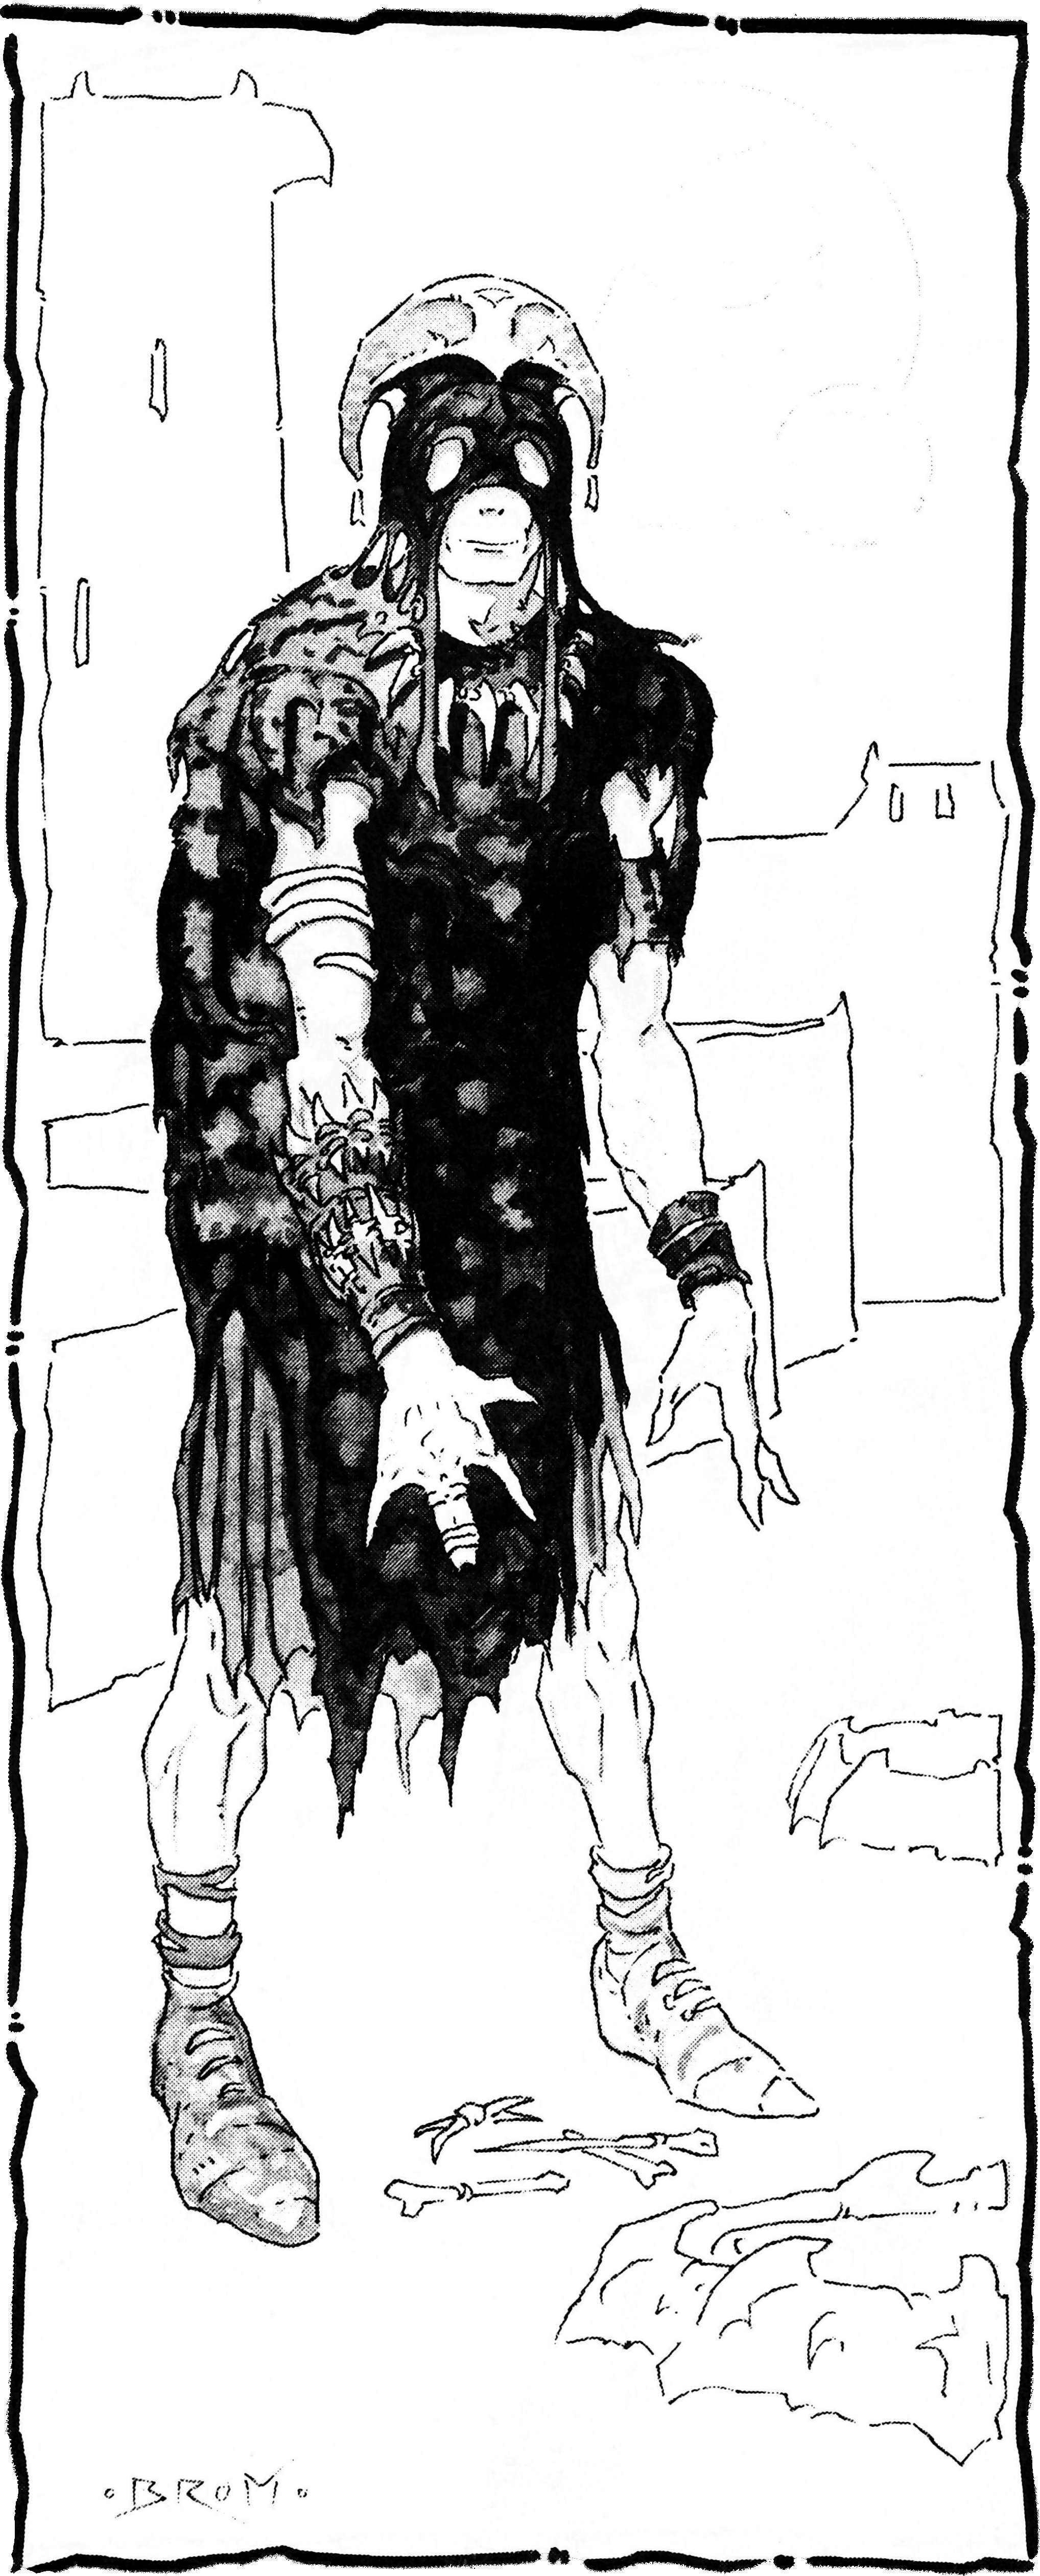
\includegraphics[width=\columnwidth]{images/wiz-1.png}
\WOTC
\end{figure}
\section{Character Progress}

DMs use adventures to offer a number of challenges (or encounters) for the characters to overcome. As the characters overcome these encounters, they should improve and gain new abilities to overcome greater challenges. The rate of encounters is called the pace of the adventure, or the pace of the campaign. \tabref{Paces of Campaign} shows how many encounters or sessions are expected for each type of campaign.

\Table{Paces of Campaign}{X R R}{
\tableheader Pace of Campaign & \tableheader Encounters per Level & \tableheader Sessions per Level\\
Rushed  &  5 encounters & 1 session \\
Fast    & 10 encounters & 2 sessions \\
Default & 12 encounters & 3 sessions \\
Slow    & 15 encounters & 4 sessions \\
Dragged & 20 encounters & 5+ sessions \\
}

Instead of the standard of using Experience Points (XP) to attain new character levels, we recommend that players gain levels based on a fixed number of sessions. This way the DM can tailor the experience based on the frequency of the sessions, e.g., if your group can only play once per month it may be better to speed up the progress of the characters.

If your group would rather use a traditional leveling system via XP, you can use \tabref{Traditional Experience and Wealth}. In this table there is the expected wealth of player characters. Use this as a guide to balance adventures, i.e., do not assume a 3rd-level character should have a 3,000 cp item.

\Table{Traditional Experience and Wealth}{lRRR}{
\tableheader ECL & \tableheader Total XP & \tableheader XP for next level & \tableheader Wealth\\
1  &         &  1,500 & 3d4 $\times$ 10 cp\\
2  &   1,500 &  3,000 & 600 cp\\
3  &   4,500 &  4,500 & 1,500 cp\\
4  &   9,000 &  6,000 & 3,000 cp\\
5  &  15,000 &  7,500 & 6,000 cp\\
6  &  22,500 &  9,000 & 9,000 cp\\
7  &  31,500 & 10,500 & 12,000 cp\\
8  &  42,000 & 12,000 & 18,000 cp\\
9  &  54,000 & 13,500 & 24,000 cp\\
10 &  67,500 & 15,000 & 30,000 cp\\
11 &  82,500 & 16,500 & 42,000 cp\\
12 &  99,000 & 18,000 & 54,000 cp\\
13 & 117,000 & 19,500 & 66,000 cp\\
14 & 136,500 & 21,000 & 90,000 cp\\
15 & 157,500 & 22,500 & 114,000 cp\\
16 & 180,000 & 24,000 & 138,000 cp\\
17 & 204,000 & 25,500 & 186,000 cp\\
18 & 229,500 & 27,000 & 234,000 cp\\
19 & 256,500 & 28,500 & 282,000 cp\\
20 & 285,000 &        & 378,000 cp\\
}

\subsubsection{Level-Dependent Benefits}
Besides the bonuses given by their character classes, all characters gain additional feats and increase their abilities from advancing in level as seen in \tabref{Level-Dependent Benefits}. This does not count a race's level adjustment---only character classes.

\textbf{Feat:} Every character gets their first feat at 1st level. At 3rd level and every other 3 levels, characters gain another feat. More information on feats on \chapref{Feats}.

\textbf{Ability Score Increase:} At 4th level and every 4 levels thereafter, the player chooses one of their character's ability scores to increase by 1 point. This improvement is permanent.

\textbf{Class Skill Max Ranks:} The maximum number of ranks a character can have in a class skill is equal to their character level +3.

\textbf{Cross-Class Skill Max Ranks:} For cross-class skills, the maximum number of ranks is one-half the maximum for a class skill.

\Table{Level-Dependent Benefits}{lccCC}{
\multirow[b]{2}{11mm}{\tableheader Character Level}
& \multirow[b]{2}{5mm}{\centering \tableheader Feat}
& \multirow[b]{2}{15mm}{\centering \tableheader Ability Score\\Increase}
& \multicolumn{2}{c}{\tableheader Max Ranks}\\
\cmidrule[0.5pt]{4-5}
&&& \tableheader Class Skill & \tableheader Cross-Class Skill\\

 1 & 1st &     &  4 & 2          \\
 2 &     &     &  5 & 2\onehalf  \\
 3 & 2nd &     &  6 & 3          \\
 4 &     & 1st &  7 & 3\onehalf  \\
 5 &     &     &  8 & 4          \\
 6 & 3rd &     &  9 & 4\onehalf  \\
 7 &     &     & 10 & 5          \\
 8 &     & 2nd & 11 & 5\onehalf  \\
 9 & 4th &     & 12 & 6          \\
10 &     &     & 13 & 6\onehalf  \\
11 &     &     & 14 & 7          \\
12 & 5th & 3rd & 15 & 7\onehalf  \\
13 &     &     & 16 & 8          \\
14 &     &     & 17 & 8\onehalf  \\
15 & 6th &     & 18 & 9          \\
16 &     & 4th & 19 & 9\onehalf  \\
17 &     &     & 20 & 10         \\
18 & 7th &     & 21 & 10\onehalf \\
19 &     &     & 22 & 11         \\
20 &     & 5th & 23 & 11\onehalf \\
}

\subsection{Gaining Experience}
Award players for combat, skills, and role-playing. Combat can be inevitable and emerging victorious in a combat should earn experience points. Skills are the way of dealing with problems without violence. Like combat, awards are only for successful attempts.

There are also some guidelines to award players experience points for their roleplay. These are based on their race, so that they are incentivized to follow the racial culture.

\subsubsection{Awards per Race}
These awards are for roleplaying some of the stereotypical aspects of athasian character races. Players should remember that races are more than just stats on their character sheets, they have culture and history which are what these stereotypes try to enforce.

The judgment of good roleplaying ultimately lies with the DM, and they must be familiar with the nuances of the character races. The communication between the DM and the players should be clear so that a good roleplaying experience can arise, and the nature of \textbf{Dark Sun} can be emphasized.

To determine the XP award for a particular action, check the correspondent table for the character's race and multiply the award by the character's effective character level (ECL). Remember that this will quicken the rate of progress of the characters.

\textbf{Aarakocra}: Aarakocras are claustrophobic. Whenever not entering a closed space becomes a hard choice, aarakocras should be rewarded for choosing their phobia over the closed space. This should not be awarded when the stakes for not entering are low.

Aarakocras are a flying race. Whenever aarakocras enter buildings through windows because they were flying high, they should get experience bonus.

\XPTable{Aarakocras}{
Enter building through window & 25 XP \\
Refuse to enter closed spaces & 100 XP \\
}

\textbf{Dwarf}: Dwarves live by their foci. A focus must take at least a week to complete. If a focus takes a least a year to complete, it becomes a major focus.

Focus can be changed in very rare circumstances. These circumstances must be agreed between the player and the DM.

\XPTable{Dwarves}{
Pursue present focus & 50 XP $\times$ days pursuing \\
Ignore present focus & -100 XP $\times$ days ignoring \\
Complete major focus & 1,000 XP \\
}

\textbf{Elf}: Roleplaying an elf is centered around trust. Elves are self-reliant and do not want to gain friendship with every character they meet. They test redeemable outsiders (in the elvish perspective) to see if they are trustworthy.

\textit{Examples of subtle tests of trust}:
\begin{itemize*}
	\item entrust with confidential information,
	\item leave a valuable item easy for taking to see the outsider takes it,
	\item ask to deliver a message or item.
\end{itemize*}

\textit{Examples of life-threatening tests of trust}:
\begin{itemize*}
	\item let themselves get captured to see if there is a rescue attempt,
	\item fake unconsciousness after a battle to see what type of care is provided,
	\item cut supplies to see if they get a fair share.
\end{itemize*}

\XPTable{Elves}{
Subtle test of trust & 25 XP \\
Life-threatening test of trust & 200 XP \\
Refuse animal or magical transport & 50 XP \\
Continuous run & 10 XP $\times$ distance in km \\
}

\textbf{Half-Elf}: Every half-elf seek acceptance among humans and elves, t hough they deny it as much as possible. Observing simple customs for the first time should award bonus experience points. These can be drinking the local ale with the elven chieftain or participating in a human wedding ritual.

If a local custom takes form of a competition, the half-elf gains bonus experience points if they perform better than any \emph{one} of the humans or elves also participating. If they perform better than \emph{all} the humans or elves, they get double the experience award.

\XPTable{Half-Elves}{
Observe human or elven custom & 25 XP \\
Better a human or elf in custom & 250 XP \\
}

\textbf{Half-Giant}: A half-giant seeks guidance and purpose in others' lifestyles. Player characters should seek to imitate the most charismatic member of the party in their racial and class customs. Whenever they do, they should be rewarded for it.

Half-giant can also look elsewhere for inspiration, imitating non-player characters and may even switch sides in an adventure. Whenever a player goes this far, they should get bonus experience points.

Whenever half-giants shift their alignment based on the events in the campaign, the DM should give them bonus experience points. This is only for appropriate shifts that are followed by a meaningful roleplay.

\XPTable{Half-Giants}{
Imitate charismatic friend & 25 XP $\times$ days imitating \\
Shift alignment per influence & 50 XP \\
}

\textbf{Halfling}: Halflings come from isolated tribes and, similar to half-elves, they want to experiment other races' customs. Unlike half-elves, their drive is curiosity, instead of trying to fit in. Whenever halflings try a  custom for the first time, no matter how trivial, they gain an experience bonus.

Their sense of belonging makes them honor bound to aid another halfling in need. This should only be rewarded when there is danger of injury or loss of life to the aiding halfling.

\XPTable{Halflings}{
Refuse money & 25 XP \\
Practice another race's custom & 50 XP \\
Eat slain foe & 50 XP \\
Aid another halfling & 100 XP \\
}

\textbf{Mul}: As a race bred exclusively for slavery, muls lack a culture similar to the other races. What they all share is the culture of labor. Whenever they exert themselves, they should be awarded bonus experience. This should only be rewarded if the exertion is meaningful to the adventure.

\XPTable{Muls}{
Heavy exertion & 10 XP $\times$ day of work \\
}

\textbf{Pterran}: Pterran culture venerates Earth Mother, so whenever pterrans celebrate her they should be rewarded. This also means that defilers are natural foes to pterrans, since they desecrate Earth Mother.

As a vibrant culture, they are curious to witness other cultures---as long as they don't harm the Earth Mother.

\XPTable{Pterrans}{
Celebration for Earth Mother & 25 XP\\
Practice another race's custom & 50 XP \\
Defeat defiler & 50 XP $\times$ defiler's CR\\
}

\textbf{Thri-Kreen}: Thri-kreen come from an empire of hunter-gatherers. Whenever they take back a slain creature for food, it should warrant experience bonus.

\XPTable{Thri-Kreens}{
Defeat creature for food & 50 XP \\
Paralyze creature & 100 XP \\
}

% \subsubsection{Awards per Class}
% Multiclass characters must choose which class to consider when receiving awards---you can only gain award for a single class.

% \textbf{\class{Barbarian}}: Barbarians are survivalists, so beyond defeating living creatures, defeating traps and natural hazards on their might alone award them bonus experience points.

% \XPTable{Barbarians}{
% Use special attack & 5 XP\\
% Use rage & 10 XP\\
% Defeat a creature & 10 XP $\times$ creature's CR\\
% Defeat trap or natural hazard & 10 XP $\times$ trap's CR\\
% }

% \textbf{\class{Bard}}: Bards gain bonus experience points for successful use of their bardic abilities. However they also gain XP for using poison against a creature---to weaken or kill the victim.

% \XPTable{Bards}{
% Use bardic music & 10 XP\\
% Use bardic knowledge & 25 XP\\
% Use poison effectively & 5 XP $\times$ creature's CR\\
% Defeat a creature & 5 XP $\times$ creature's CR\\
% Obtain treasure & 5 XP $\times$ value in cp\\
% }

% \textbf{\class{Cleric}}: Using elements with finesse and flair to overcome an obstacle should reaward clerics bonus experience points.

% \XPTable{Clerics}{
% Use domain power & 10 XP\\
% Use element creatively & 50 XP\\
% Cast spell & 5 XP $\times$ spell level\\
% Cast Healing spell & 10 XP $\times$ spell level\\
% Turn/rebuke undead & 25 XP $\times$ undead's CR\\
% Destroy/command undead & 50 XP $\times$ undead's CR\\
% Create magic item & 200 XP\\
% }

% \textbf{\class{Druid}}:

% \XPTable{Druids}{
% Cast spell & 5 XP $\times$ spell level\\
% Case Healing spell & 10 XP $\times$ spell level\\
% Use wild empathy & 25 XP\\
% Use wild shape & 10 XP\\
% Defeat defiler & 50 XP $\times$ defiler's CR\\
% Create magic item & 200 XP\\
% }

% \textbf{\class{Fighter}}: The fighter's role in society is about mass warfare, so being a good soldier during these times will award her additional experience points. Fighters do not gain experience points for spending weeks in reserve, even if they're commanding followers.

% \XPTable{Fighters}{
% Use special attack & 5 XP\\
% Defeat a creature alone & 5 XP $\times$ creature's CR\\
% Defeat a creature with a group & 10 XP $\times$ creature's CR\\
% Follow commands in battle & 25 XP\\
% Command a battle & 50 XP\\
% Build a war machine & 100 XP\\
% }

% \textbf{\class{Gladiator}}: Gladiators desire to be in the spotlight of an arena, to be the victor of a duel. Therefore, they receive additional experience points for defeating creatures in an arena without outside aid. The glory must be their alone.

% \XPTable{Gladiators}{
% Use special attack & 5 XP\\
% Use gladiatorial perfomance & 10 XP\\
% Defeat a creature & 5 XP $\times$ creature's CR\\
% Defeat a creature alone in an arena & 10 XP $\times$ creature's CR\\
% }

% \textbf{\class{Psion}}:

% \XPTable{Psions}{
% Defeat a psionic creature & 5 XP $\times$ creature's CR\\
% Research new psionic knowledge & 50 XP\\
% Manifest a power & 5 XP $\times$ power level\\
% Manifest a power to avoid combat & 10 XP $\times$ power level\\
% Create psionic item & 200 XP\\
% }

% \textbf{\class{Psychic Warrior}}:

% \XPTable{Psychic Warriors}{
% Defeat a creature & 5 XP $\times$ creature's CR\\
% Defeat a psionic creature & 5 XP $\times$ creature's CR\\
% Manifest a power & 5 XP $\times$ power level\\
% }

% \textbf{\class{Ranger}}: Rangers track their foes and hunt favored enemies. Accomplishing these taks award them additional experience points.

% \XPTable{Ranger}{
% Cast spell & 5 XP $\times$ spell level\\
% Defeat a creature & 5 XP $\times$ creature's CR\\
% Defeat a creature in a favorite territory & 5 XP $\times$ creature's CR\\
% Defeat a favorite enemy & 10 XP $\times$ enemy's CR\\
% Track a creature & 10 XP\\
% Track a creature in a favorite territory & 10 XP\\
% Track a favorite enemy & 10 XP\\
% Use wild empathy & 25 XP\\
% }

% \textbf{\class{Rogue}}:

% \XPTable{Rogue}{
% Defeat a creature & 5 XP $\times$ creature's CR\\
% Disable trap & 25 XP $\times$ trap's CR\\
% Obtain treasure & 5 XP $\times$ value in cp\\
% Obtain treasure for patron & 5 XP $\times$ value in cp\\
% Use sneak attack & 5 XP\\
% }

% \textbf{\class{Templar}}:

% \XPTable{Templar}{
% Cast spell & 5 XP $\times$ spell level\\
% Use secular authority on slave & 5 XP\\
% Use secular authority on freeman & 10 XP\\
% Use secular authority on noble & 25 XP\\
% Use secular authority on templar & 50 XP\\
% Fulfill sorcerer-king's mission & 100 XP\\
% }

% \textbf{\class{Wilder}}:

% \XPTable{Wilders}{
% Defeat a psionic creature & 5 XP $\times$ creature's CR\\
% Create psionic item & 200 XP\\
% Surge without enervation & 10 XP $\times$ bonus level\\
% Manifest a power & 5 XP $\times$ power level\\
% Manifest a power to avoid combat & 10 XP $\times$ power level\\
% }

% \textbf{\class{Wizard}}: Preservers and defilers serve different roles in the athasian society. Preservers want to remain hidden from the eyes of the templars, so they gain additional experience points for keeping spellcasting secret. Defilers on the other hand are aligned with the \emph{status quo} and are awarded additional experience points for carrying out the business of their sorcerer-monarchs.

% \XPTable{Wizards}{
% Cast spell & 5 XP $\times$ spell level\\
% Cast spell for sorcerer-king (defiler) & 5 XP $\times$ spell level\\
% Find new spell to spellbook & 50 XP $\times$ spell level\\
% Keep spellcasting secret (preserver) & 25 XP\\
% Create magic item & 200 XP\\
% }

\subsubsection{Awards for Skill Check}
Skill checks represent nonviolent challenges in the game. To determine the XP award for a successful skill check, follow these steps:

\begin{enumerate*}
	\item Calculate the adjusted Difficulty Class (DC) of the check. It is equal to the skill check's DC minus any racial bonus the character has in that check.
	\item Use \tabref{Experience Awards from Skill Checks} to cross-reference the campaign's pace with the adjusted DC to find the XP award.
\end{enumerate*}
 
Only successful checks award XP. Checks with adjusted DC lower than 10 do not give XP. The award is not based on the check's result.

Opposed checks do not have Difficulty Class. For the purposes of experience awards, they are considered to have a DC equal to a roll of 12. For example, a barbarian with a Hide modifier of +4 would be awarded 50 XP if they pass a Hide check DC 16---regardless of the result of the barbarian's Hide check or any opposed Spot check.

\Table{Experience Awards from Skill Checks}{L *5C}{
\rowcolor{white}
\multirow[c]{2}{1cm}{\tableheader Adjusted DC} & \multicolumn{5}{c}{\tableheader Experience Points Award}\\
\cmidrule[0.5pt]{2-6}
& \tableheader Rushed & \tableheader Fast & \tableheader Normal & \tableheader Slow & \tableheader Dragged \\

10--11 & 25 & 15 & 10 & 8 & 5 \\
12--14 & 60 & 30 & 25 & 20 & 15 \\
15--19 & 120 & 60 & 50 & 40 & 30 \\
20--24 & 250 & 120 & 100 & 80 & 60 \\
25--29 & 600 & 300 & 250 & 200 & 150 \\
30--39 & 1,200 & 600 & 500 & 400 & 300 \\
40--49 & 2,400 & 1,200 & 1,000 & 800 & 600 \\
50+ & 6,000 & 3,000 & 2,500 & 2,000 & 1,500 \\
}

\subsubsection{Awards for Combat}
When the players defeat the enemy in battle, they earn experience points. Only characters who take part in the battle should gain XP. Characters who died before the combat, or did not participate for any other reason, should not be awarded.

To determine the XP award for a combat, follow these steps.
\begin{enumerate*}
	\item Determine each character's effective character level (ECL).
	\item For each monster or trap defeated, determine its Challenge Rating (CR).
	\item Use \tabref{Experience Awards from Combats} to cross-reference the campaign's pace with the CR of each monster or trap to find the base XP award.
	\item Divide the base XP award by the number of characters in the party.
	\item Add up all the XP awards for all the monsters or traps the character helped defeat.
	\item Repeat the process for each character.
\end{enumerate*}

Creatures summoned or that otherwise are related to an enemy's ability (such as animal companion) do not award XP. These abilities are already taken into account in the enemy's CR.

\Table{Experience Awards from Combats}{X *{5}{C}} {
\rowcolor{white}
\multirow[l]{2}{1cm}{\tableheader Challenge Rating} & \multicolumn{5}{c}{\tableheader Experience Points Award (per monster)}\\
\cmidrule[0.5pt]{2-6}
& \tableheader Rushed & \tableheader Fast & \tableheader Normal & \tableheader Slow & \tableheader Dragged \\

1 & 1,200 & 600 & 500 & 400 & 300 \\
2 & 2,400 & 1,200 & 1,000 & 800 & 600 \\
3 & 3,600 & 1,800 & 1,500 & 1,200 & 900 \\
4 & 4,800 & 2,400 & 2,000 & 1,600 & 1,200 \\
5 & 6,000 & 3,000 & 2,500 & 2,000 & 1,500 \\
6 & 7,200 & 3,600 & 3,000 & 2,400 & 1,800 \\
7 & 8,400 & 4,200 & 3,500 & 2,800 & 2,100 \\
8 & 9,600 & 4,800 & 4,000 & 3,200 & 2,400 \\
9 & 10,800 & 5,400 & 4,500 & 3,600 & 2,700 \\
10 & 12,000 & 6,000 & 5,000 & 4,000 & 3,000 \\
11 & 13,200 & 6,600 & 5,500 & 4,400 & 3,300 \\
12 & 14,400 & 7,200 & 6,000 & 4,800 & 3,600 \\
13 & 15,600 & 7,800 & 6,500 & 5,200 & 3,900 \\
14 & 16,800 & 8,400 & 7,000 & 5,600 & 4,200 \\
15 & 18,000 & 9,000 & 7,500 & 6,000 & 4,500 \\
16 & 19,200 & 9,600 & 8,000 & 6,400 & 4,800 \\
17 & 20,400 & 10,200 & 8,500 & 6,800 & 5,100 \\
18 & 21,600 & 10,800 & 9,000 & 7,200 & 5,400 \\
19 & 22,800 & 11,400 & 9,500 & 7,600 & 5,700 \\
20 & 24,000 & 12,000 & 10,000 & 8,000 & 6,000 \\
}

\subsection{Alternative Progress}
Here are presented two alternative ways to change the experience progress in your campaign: partial progression and tiered powers. Each variant rule tries to delay (or halt) level progress. You are not required to use any of those variant rules to run a {\tableheader Dark Sun} adventure, since these are designed to tackle different problems and different tastes.

\subsubsection{Partial Progression}
Characters gain experience and that experience may be represented as a new level. But that is not the only way to mark character growth. Here we present some alternate rules for expending experience points. These options may be adequate for adventures that don't strive to get into high levels. Maybe you want for the characters to stay in the same level for longer than normal. With these options, they can get meaningful progression without receiving an actual level.

In \tabref{Partial Progression}, you can see the benefits and their costs. Some benefits are intentionally left out of the table, such as general feats or extra spell slots. Those benefits are too close to a new level, so it would be more meaningful to give an actual level.

\Table{Partial Progression}{XX}{
\tableheader Benefit & \tableheader XP Cost (per ECL)\\
1 skill point        & 100 XP\\
1 skill feat         & 200 XP\\
1 racial feat        & 300 XP\\
1 regional feat      & 300 XP\\
1 item creation feat & 500 XP\\
}

\textbf{Skill Point:} You gain one skill point, just as the skill points gained by acquiring a new level. You can't have more ranks than you are allowed for your level. Spending this skill point on a cross-class skill still gets your character \onehalf rank in that skill. For more information on skill points, see \chapref{Skills}.

\textbf{Feats:} You may purchase a new feat, granted you have its prerequisites. You can only purchase some types of feats: item creation feats, racial feats, regional feats, and skill feats. For more information on these types of feats, see \chapref{Feats}.

\subsubsection{Tiered Powers}
There is a natural imbalance towards magical (and psionic) powers. So much so that the whole system is balanced around wonderous items, and it is expected to have spellcasters in an adventuring group. But at higher levels, this imbalance in power can become frustrating for both DMs and players, as the powers become increasingly more complex and game-changing.

In \tabref{Tiered Powers}, you can see the level adjustment based on the maximum spell level or power level available for a manifester or spellcaster. This means that a 17th-level human wizard should be equivalent to a 19th-level character---she has access to 9th-level magic and thus has a +2 level adjustment. An elf psychic warrior of the same level (17th) should be equivalent to a 18th-level character---6th-level psionic powers grant +1 level adjustment.

\Table{Tiered Powers}{lXc}{
\tableheader Tier & \tableheader Maximum Spell/Power Level Available & \tableheader Total Level Adjustment \\
I   & 1st--3rd & +0 \\
II  & 4th--6th & +1 \\
III & 7th--9th & +2 \\
}

In an already running adventure, a character that will change their tier should only advance another level after gaining enough experience for two whole levels. For instance, Jozan is a 6th-level human cleric. In order for him to get his 7th level (and 4th-level spells), he must gain enough XP to advance to an effective 8th character level. Once the character makes a tier breakthrough, he advances normally with his level adjustment and new effective character level until another breakthrough must be made. So from his 7th level to 12th level, Jozan advances with a +1 level adjustment. After he becomes a 12th-level cleric (13 ECL), he should again acquire enough XP to advance two character levels in order to gain access to 7th-level spells---this time to an effective 15th character level. After that, he advances normally again with his +2 level adjustment.
\section{Multiclass Characters}
A character may add new classes as he or she progresses in level, thus becoming a multiclass character. The class abilities from a character's different classes combine to determine a multiclass character's overall abilities. Multiclassing improves a character's versatility at the expense of focus.

\subsection{Prerequisites}
To qualify for a new class, you must meet the ability score prerequisites for both your current class and your new one, as shown in \tabref{Multiclassing Prerequisites}. For example, a barbarian who decides to multiclass into the druid class must have Wisdom score of 15 or higher, and both Strength and Constitution scores of 13 or higher. Without the full training that a beginning character receives, you must be a quick study in your new class, having a natural aptitude that is reflected by higher-than-average ability scores.

\Table{Multiclassing Prerequisites}{lL}{
\tableheader Class & \tableheader Ability Score Minimum \\
Barbarian       & Strength 13, Constitution 13 \\
Bard            & Charisma 13, Dexterity or Intelligence 13 \\
Cleric          & Wisdom 13, Charisma 13 \\
Druid           & Wisdom 15 \\
Fighter         & Constitution 13, Strength or Dexterity 13 \\
Gladiator       & Strength 13, Intelligence or Charisma 13 \\
Psion           & Wisdom 13, Constitution or Intelligence 13 \\
% Psychic Warrior & Strength or Dexterity 13, Wisdom 13 \\
Ranger          & Wisdom 13, Strength or Dexterity 13 \\
Scout           & Dexterity 13, Strength or Wisdom 13 \\
Templar         & Wisdom 13, Charisma 13 \\
Thief           & Dexterity 13, Intelligence or Charisma 13 \\
% Wilder          & Charisma 15 \\
Wizard          & Intelligence 15 \\
}

\subsection{Class And Level Features}
As a general rule, the abilities of a multiclass character are the sum of the abilities of each of the character's classes.

\textbf{Level:} ``Character level'' is a character's total number of levels. It is used to determine when feats and ability score boosts are gained.

``Class level'' is a character's level in a particular class. For a character whose levels are all in the same class, character level and class level are the same.

\textbf{Hit Points:} A character gains hit points from each class as his or her class level increases, adding the new hit points to the previous total.

\textbf{Base Attack Bonus:} Add the base attack bonuses acquired for each class to get the character's base attack bonus. A resulting value of +6 or higher provides the character with multiple attacks.

\textbf{Saving Throws:} Add the base save bonuses for each class together.

\textbf{Skills:} If a skill is a class skill for any of a multiclass character's classes, then character level determines a skill's maximum rank. (The maximum rank for a class skill is 3 + character level.)

If a skill is not a class skill for any of a multiclass character's classes, the maximum rank for that skill is one-half the maximum for a class skill.

\textbf{Class Features:} A multiclass character gets all the class features of all his or her classes but must also suffer the consequences of the special restrictions of all his or her classes.

In the special case of turning undead, both clerics and experienced templars have the same ability. If the character's templar level is 4th or higher, her effective turning level is her cleric level plus her templar level.

In the special case of uncanny dodge, experienced barbarians, experienced gladiators, experienced scouts, and experienced thieves have the same ability. When a barbarian/rogue would gain uncanny dodge a second time (for her second class), she instead gains improved uncanny dodge, if she does not already have it. Her barbarian and rogue levels stack to determine the rogue level an attacker needs to flank her.

\textbf{Feats:} A multiclass character gains feats based on character levels, regardless of individual class level

\textbf{Ability Increases:} A multiclass character gains ability score increases based on character level, regardless of individual class level.

\textbf{Spells:} The character gains spells from all of his or her spellcasting classes and keeps a separate spell list for each class. If a spell's effect is based on the class level of the caster, the player must keep track of which class's spell list the character is casting the spell from.

\textbf{Power Points:} If you have levels in more than one psionic class, you combine your power points from each class to make up your reserve. You can use these power points to manifest powers from any psionic class you have.

While you maintain a single reserve of power points from your class, race, and feat selections, you are still limited by the manifester level you have achieved with each power you know.

\section{Alternate Class Features}
Choosing a class fixes key aspects of a character: their role, their abilities, and their attack and save bonuses. However, you can change a class feature to provide a new experience. Variant versions of several of class features are presented below. If you prefer the variant to the standard class feature, ask your game master if he approves of your swapping out your class feature for the variant version.

These alternate class features can exist side by side with the standard class features---some bards might work alone while their comrades favor having contacts all over Athas---or can completely replace the standard features. The balance between the standard class features and the alternate features is up to the game master.

The description of alternate class features is the following.

\subsection{Class Name}
\subsubsection{Alternate Class Feature Name}
A general description of the ability.

\textbf{Special Requirement:} Any special requirements that you must meet before selecting the alternative class feature. Many of the alternative class features described here require ranks of a skill. Since skill ranks are purchased before class features are selected, you can meet this requirement at the same level that you gain the alternative class feature.

\textbf{Level:} The alternative class feature can be selected only at this level. In some cases, different levels might be given for different classes.

\textbf{Replaces:} The ability that you must sacrifice to gain the alternative class feature.

\textbf{Benefit:} The mechanical effects of the new ability.

\subsection{Bard}
\AlternateClassFeature{Contact}
{Instead of relying on their own wits like a traditional bard, a \emph{draqoman} relies on the help of others more capable in specific matters. Draqomen serve as guides and translators for newcomers to the cities. Local laws and customs vary by location, and a local resident who knows the city like the back of his hand and can call in a favor if necessary is definitely worth his pay. A draqoman will usually be loyal as long as he is paid and fed well. Mistreat your draqoman and you will soon find yourself on the wrong end of someone's blade or in the prisons run by the templars.}
{\skill{Diplomacy} 2 ranks, \skill{Gather Information} 4 ranks, \skill{Knowledge} (local) 4 ranks.}
{6th, 11th, and 16th.}
{You do not gain quick thinking, or its improvements at 11th and 16th levels.}
{
	You gain the trust of a non-player character he can rely on when the time comes. You can ask for a favor once per week per contact. Contacts come in three varieties, one of which you must choose: influence contacts, skill contacts, and trade contacts (see \hyperref[sec:contacts]{Contacts}).

	You gain one additional use of contact at 11th level, and another again at 16th level.
}

\begin{figure*}[t!]
\centering
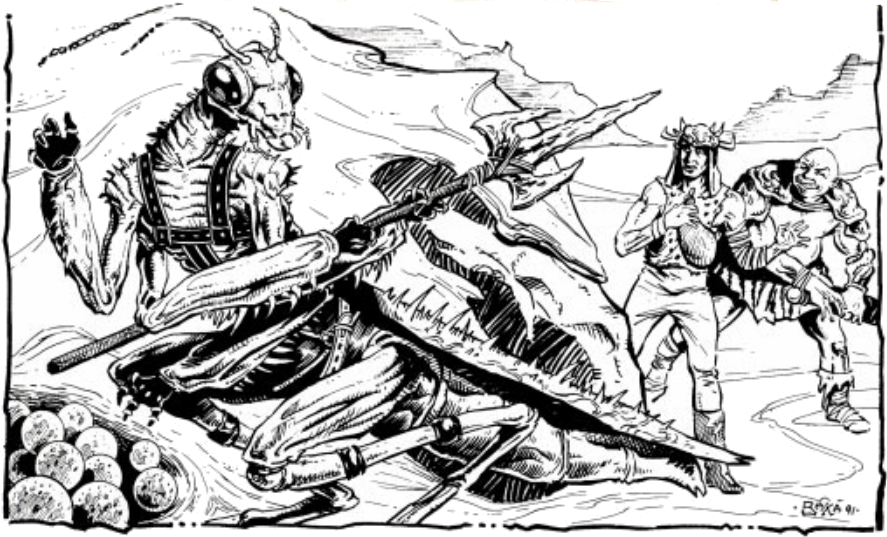
\includegraphics[width=\textwidth-1cm]{images/thrikreen-1.png}
\WOTC
\end{figure*}
\AlternateClassFeature{Procurer}
{To all outward appearances, procurers seem to be everyday elf traders. They conduct their thefts in secret, using normal trading practices to cover their filching activities. These elves usually work for elven merchant houses, filling the market stalls with goods stolen from other merchants, nobles, free citizens, templars, and even the sorcerer-kings.}
{Elf or half-elf.}
{2nd.}
{You do not gain streetsmart.}
{
	You gain +5 in \skill{Search} checks to find secret doors.
}

\subsection{Fighter}
\AlternateClassFeature{Reckless}
{The eagle knights are among the most brutal and fanatical Draji warriors. They are more than willing to charge headfirst into battle for the glory of Draj and their god-king.}
{Must be trained by the Draji army.}
{10th.}
{You do not gain a bonus feat.}
{
	When using the attack or full attack option, you can subtract a number from his Armor Class and add this number to damage inflicted on successful attacks. This number may not exceed your base attack bonus. The Armor Class penalty and damage bonus last until the your next standard action.
}
\AlternateClassFeature{Savage Hunter}
{The savage hunter is the most common elf warrior type, serving as both a tribal defender and an important food provider. Respected by others of the tribe, the savage hunter uses the same skills to hunt prey and to fight outsiders and other threats to the tribe. The ways of the city-states are alien to these wilderness warriors, for they are only at home in the wastes when on a hunt.}
{Elf or half-elf.}
{1st.}
{You do not gain a bonus feat.}
{
	You gain \feat{Track} as a bonus feat. You add \skill{Survival} to your fighter class skills.
}

\AlternateClassFeature{Tik-Tik}
{Larger and less dexterous than most other kreen, the ``hunter-of-hunters'' guards the weaker members of the pack. In dangerous territory, Tik-Tik rarely hunt, unless the pack's normal hunters are spread too thinly or have been incapacitated by enemies.}
{Thri-kreen.}
{1st.}
{You do not gain a bonus feat.}
{
	Your natural armor bonus increases by 1 (+3 total). You add \skill{Survival} to your fighter class skills.
}

\subsection{Gladiator}
\AlternateClassFeature{Flexibility Adjustment}
{These gladiators adjust their armor to improve their reflex capabilities instead of increasing the area it protects.}
{}
{5th, 10th, 15th, and 20th.}
{You do not gain armor optimization, or its improvements at 10th, 15th, and 20th levels.}
{
	You improve the maximum Dexterity bonus and reduce the armor check penalty by 1, whenever you are wearing any armor you are proficient with.

	At every five levels thereafter, the improvement increases by 1 (2 at 10th, 3 at 15th, and 4 at 20th level).
}
\AlternateClassFeature{Lighten Load}
{By changing slightly the armor to their own bodies, these gladiators can move faster with a heavier armor.}
{}
{5th.}
{You do not gain armor optimization.}
{
	You treat the armor as one category lighter (e.g. medium armor is treated as light armor), whenever you are wearing any armor you are proficient with.
}

\subsection{Psion}
\AlternateClassFeature{Contact}
{The cities of Athas are filled with intrigue, treachery, and double-dealing. In this setting, information is a weapon that may be wielded against one’s enemies. The auditor’s job description ranges from information broker to psionic assassin. In most cities, the templars have auditors working for them. Other auditors are members of the Veiled Alliance, criminal gangs, or are employed by the merchant dynasties.}
{\skill{Diplomacy} 2 ranks, \skill{Gather Information} 4 ranks, \skill{Knowledge} (local) 4 ranks.}
{1st, 5th, 10th, 15th, and 20th.}
{You do not gain any bonus feat.}
{
	You gain the trust of a non-player character he can rely on when the time comes. You can ask for a favor once per week per contact. Contacts come in three varieties, one of which you must choose: influence contacts, skill contacts, and trade contacts (see \hyperref[sec:contacts]{Contacts}).

	You gain one additional use of contact at 5th level and every four levels thereafter (2 contacts at 5th, 3 at 9th, 4 at 13th, 5 at 17th).
}

\AlternateClassFeature{Tekchakak}
{The tekchakak is devoted to the preservation and prosperity of clutch and pack. These psionicists use their abilities to support their clutchmates and packmates, helping to find prey and to defend compatriots against raiders and predators. Within a
thri-kreen pack, the tekchakak offers advice, guidance, and teaching in addition to active support through their psionic abilities.}
{Thri-kreen.}
{1st.}
{You do not gain a bonus feat.}
{
	You no longer have alien mind (see \chapref{Character Races}). You add \skill{Survival} to your psion class skills.
}

\subsection{Ranger}
\AlternateClassFeature{Desert Runner}
{Desert runners are elves that have devoted themselves to the run, pushing themselves to the limit of Elven running ability. They are the scouts and messengers of a tribe. They run ahead of the rest, or alone through the desert to deliver important messages or items between clans with the greatest of speed. They are also some of the more competent hunters of the tribe able to track quarry silently while moving quickly through the desert.}
{Elf or half-elf.}
{4th.}
{You do not gain an animal companion.}
{
	You gain +1 bonus per ranger level on all \skill{Concentration} checks related to the elf run ability, and all other checks to continue running. This includes skill checks to avoid tripping or falling and saving throws to resist effects that would directly slow or impede movement (such as a Will save to resist a \spell{slow} spell). It does not however include indirectly related checks, such as a \skill{Spot} check to notice a pit trap.

	You gain +3 meters of land speed while wearing no armor or light armor, and not carrying heavy load. Your speed increases by 3 meters for every three ranger levels thereafter (+6 m at 7th, +9 m at 10th, +12 m at 13th, +15 m at 16th, and +18 m at 19th).

	You gain +1 AC dodge bonus when running. This bonus increases by 1 for every three ranger levels thereafter (+2 at 7th, +3 at 10th, +4 at 13th, +5 at 16th, and +6 at 19th).

	\emph{Desert runner} is a psi-like ability.
}
\AlternateClassFeature{Elf Favored Enemy}
{These insectoid hunters love the taste of elf flesh, and they prey upon the desert runners whenever the  opportunity presents itself. In order to combat the threat posed by the fast, strong, and cunning thri-kreen, a special class of desert runner has developed---the thri-kreen slayer.}
{Elf or half-elf.}
{1st.}
{You do not gain favored enemy.}
{
	You narrow down your choice of favorire enemy to thri-kreen. You gain a +3 bonus on \skill{Hide}, \skill{Listen}, \skill{Move Silently}, \skill{Spot}, and \skill{Survival} checks when using these skills against creatures of this race. Likewise, you get a +3 bonus on weapon damage rolls against such creatures.

	Each time you gain a new favored enemy and you choose to increase your bonus against thri-kreen, it increases by 3.
}
\AlternateClassFeature{Salvage}
{The kik has fully turned away from the life as a hunter and instead embraced the life of a raider, known in the language of the thri-kreen as a kik. The kik are in many ways more barbaric then the average kreen who roam the Tablelands, though they are not as feral as their cousins the trin.}
{Thri-kreen, \skill{Search} 5 ranks, \skill{Survival} 5 ranks.}
{7th.}
{You do not gain woodland stride.}
{
	You can make a \skill{Search} check to salvage destroyed caravans and vehicles. If the check succeeds, you earn ceramic pieces by the amount indicated on \tabref{Salvage Vehicle}, either by selling the salvaged parts or using them to offset the cost of other items.

	A particular vehicle can be successfully salvaged only once. Any further attempts to salvage the wreckage fail automatically.

	\Table{Salvage Vehicle}{Xccc}{
	\tableheader Vehicle Size & \tableheader Time & \tableheader \skill{Search} DC & \tableheader cp Earned\\
	Large or smaller & 15 min. & 10 & 10\\
	Huge & 30 min. & 15 & 20\\
	Gargantuan & 1 h & 20 & 30\\
	Colossal & 3 h & 25 & 40\\
	}
}
\AlternateClassFeature{Sand Chitin}
{Usually selected from those thri-kreen that are slightly smaller and quicker, these kreen are trained extensively in the lore of the hunt and the way of stealth, honing their natural skills beyond those of the norm of their kind.}
{Thri-kreen.}
{1st.}
{You do not gain wild empathy.}
{
	Your racial \skill{Hide} bonus increases by 2 (+6 total). For every four ranger levels thereafter, it increases by another 2 (+8 at 5th, +10 at 9th, +12 at 13th, and +14 at 17th).
}

\subsection{Rogue}
\AlternateClassFeature{Death Attack}
{The Shadows are a mysterious elf tribe of which legends and bard's tales are spun. This secretive network of elves specializes in covert and illegal operations---espionage, assassination, extortion, theft, smuggling and black market trading, to name a few. References of the shadows go back hundreds of years, and some claim they have always been around.}
{Elf, any Evil alignment, \skill{Spot} 3 ranks.}
{3rd.}
{You do not gain trap sense.}
{
	If a rogue studies his victim for 3 rounds and then makes a sneak attack with a melee weapon that successfully deals damage, the sneak attack has the additional effect of possibly either paralyzing or killing the target (rogue's choice). While studying the victim, the rogue can undertake other actions so long as his attention stays focused on the target and the target does not detect the rogue or recognize the rogue as an enemy. If the victim of such an attack fails a Fortitude save (DC 10 + \onehalf the rogue's class level + the rogue's Int modifier) against the kill effect, she dies. If the saving throw fails against the paralysis effect, the victim is rendered helpless and unable to act for 1d6 rounds plus 1 round per level of the rogue. If the victim's saving throw succeeds, the attack is just a normal sneak attack. Once the rogue has completed the 3 rounds of study, he must make the death attack within the next 3 rounds.

	If a death attack is attempted and fails (the victim makes her save) or if the rogue does not launch the attack within 3 rounds of completing the study, 3 new rounds of study are required before he can attempt another death attack.
}

\subsection{Templar}
\AlternateClassFeature{Badna's Chosen}
{Templars of Raam have been told that their divine powers stem from an entity called Badna. Most templars know or at least suspect that Badna is a fictional being created by Abalach-Re to suppress the people of Raam.}
{\skill{Knowledge} (religion) 5 ranks, must be from the templarate of Raam.}
{8th.}
{To select this class feature, you must permanently sacrifice one of your 4th-level spell slots.}
{
	You always act in the surprise round, but you permanently lose 2 points of Wisdom.
}
\AlternateClassFeature{Hamanu's Intervention}
{Urikite templars wear yellow robes, and as they rise in status strands of metal are woven into their sleeves and they receive Hamanu's personal attention. Under the tutelage of Hamanu, his templars excel in the art of combat and they can call upon their liege to power their magic or blows.}
{\skill{Knowledge} (warcraft) 4 ranks, must be from the templarate of Urik.}
{6th or any even-numbered higher level.}
{To select this class feature, you must permanently sacrifice one of your 3rd-level spell slots.}
{
	Once per day, as a move action, you may choose between +4 bonus on caster level to the next spell you cast or make your next melee attack an automatic threat (roll to determine if the attack is a critical hit).

	You may select this ability multiple times. Each time you must sacrifice another 3rd-level spell slot.

	\emph{Hamanu's intervention} is a spell-like ability.
}
\AlternateClassFeature{Nibenay's Diligence}
{The Nibenese templarate consists of women, all wedded to the Shadow King. Disciplined, educated and trained in the arts of war, the templar-wives fit perfectly into Nibenay's highly autocratic structured system of government.}
{\skill{Knowledge} (warcraft) 5 ranks, must be from the templarate of Nibenay.}
{8th.}
{To select this class feature, you must permanently sacrifice one of your 4th-level spell slots.}
{
	You can take 10 on \skill{Concentration} checks to cast spells defensively.
}
\AlternateClassFeature{Oba's Truth}
{The disciples of the Oba follow their own rites and traditions that are as ancient as those of the people of Gulg. Lalali-Puy's templars  The queen allows for templars to be dispatched to a residential dagada at the request of the dagada's leader. This request usually comes when an ambo is fearful for the security of his dagada or suspicious of an illegal activity, such as smuggling or magic use.}
{\skill{Knowledge} (nature) 7 ranks, must be from the templarate of Gulg.}
{10th.}
{To select this class feature, you must permanently sacrifice one of your 5th-level spell slots.}
{
	Once per day, you may poison a creature with a touch attack. That creature becomes infused with poison for 24 hours. If the creature tells a lie, it suffers the effect of the poison with no saving throw. The initial damage is 2d6 Con, and the secondary damage is 1d6 Con. Casting \spell{neutralize poison} or \spell{heal} will remove the poison from the victim's body.

	\emph{Oba's truth} is a spell-like ability.
}
\AlternateClassFeature{Ral's Convergence}
{For more than a thousand years, the moon priests have served Tectuktitlay, the king of Draj. Dressed in blue robes, with a yellow moon in front and in the back of their robes, the Moon Priests are responsible for the administration of the Temples of Ral and Guthay, as well as being the lead organizers of the sacrifices on the Great Pyramid.}
{\skill{Knowledge} (nature) 5 ranks, must be from the templarate of Draj.}
{8th.}
{To select this class feature, you must permanently sacrifice one of your 4th-level spell slots.}
{
	Once per day, you may reroll one d20 roll that they have just made. You must keep the result of the second roll, even if it's worse than the original roll.

	\emph{Ral's convergence} is a spell-like ability.
}

% Tyr
% Balic
% Kurn
% Eldaarich


% \AlternateClassFeature{Bureau Specialization}
% {}
% {Must be from the templarate of Tyr.}
% {8th and 12th.}
% {To select this class feature, you must permanently sacrifice one of your 4th-level spell slots, then another 6th-level spell slot at 12th level.}
% {Choose a templar class skill. You gain +3 bonus on checks of the chosen skill at 8th level.

% At 12th level, this bonus increases to +6 and you can take 10 even if stress and distraction would normally prevent you from doing so.}

\subsection{Wilder}
\AlternateClassFeature{Psionic Ritual}
{Bereft of formal training in the Way, psionically talented individuals from the tribal and nomadic peoples of the Tablelands and beyond must make do with their own understanding of the psionic arts. Seen by formally trained psions as an aberration of proper psionic practice, these self trained individuals can sometimes produce effects that leave their detractors speechless.}
{\skill{Profession} (herbalist) 4 ranks, \skill{Survival} 4 ranks.}
{7th.}
{You do not improve wild surge at 7th level.}
{
	Once per day, you can perform such a ritual to temporarily increase your Will. Each psionic ritual is unique, being of your own design, but all take one hour to complete and require a DC 20 \skill{Concentration} check. If the ritual is successful, you gain 1d4+1 temporary power points over and above your normal maximum. These power points remain available for one day or until they are used.
}

\subsection{Wizard}
\AlternateClassFeature{Exegete}
{As a result of their endless research and studies, arcanists end up knowing a little about a lot of different things. They are consulted often, becoming experts and advisers for their tribes.}
{Elf, \skill{Knowledge} (history) 10 ranks.}
{10th.}
{You do not gain a bonus feat.}
{
	You are considered to be trained in all forms of Knowledge and can choose to take 10 in \skill{Knowledge} checks which you have at least 10 ranks in.
}

\begin{figure*}[t!]
\centering
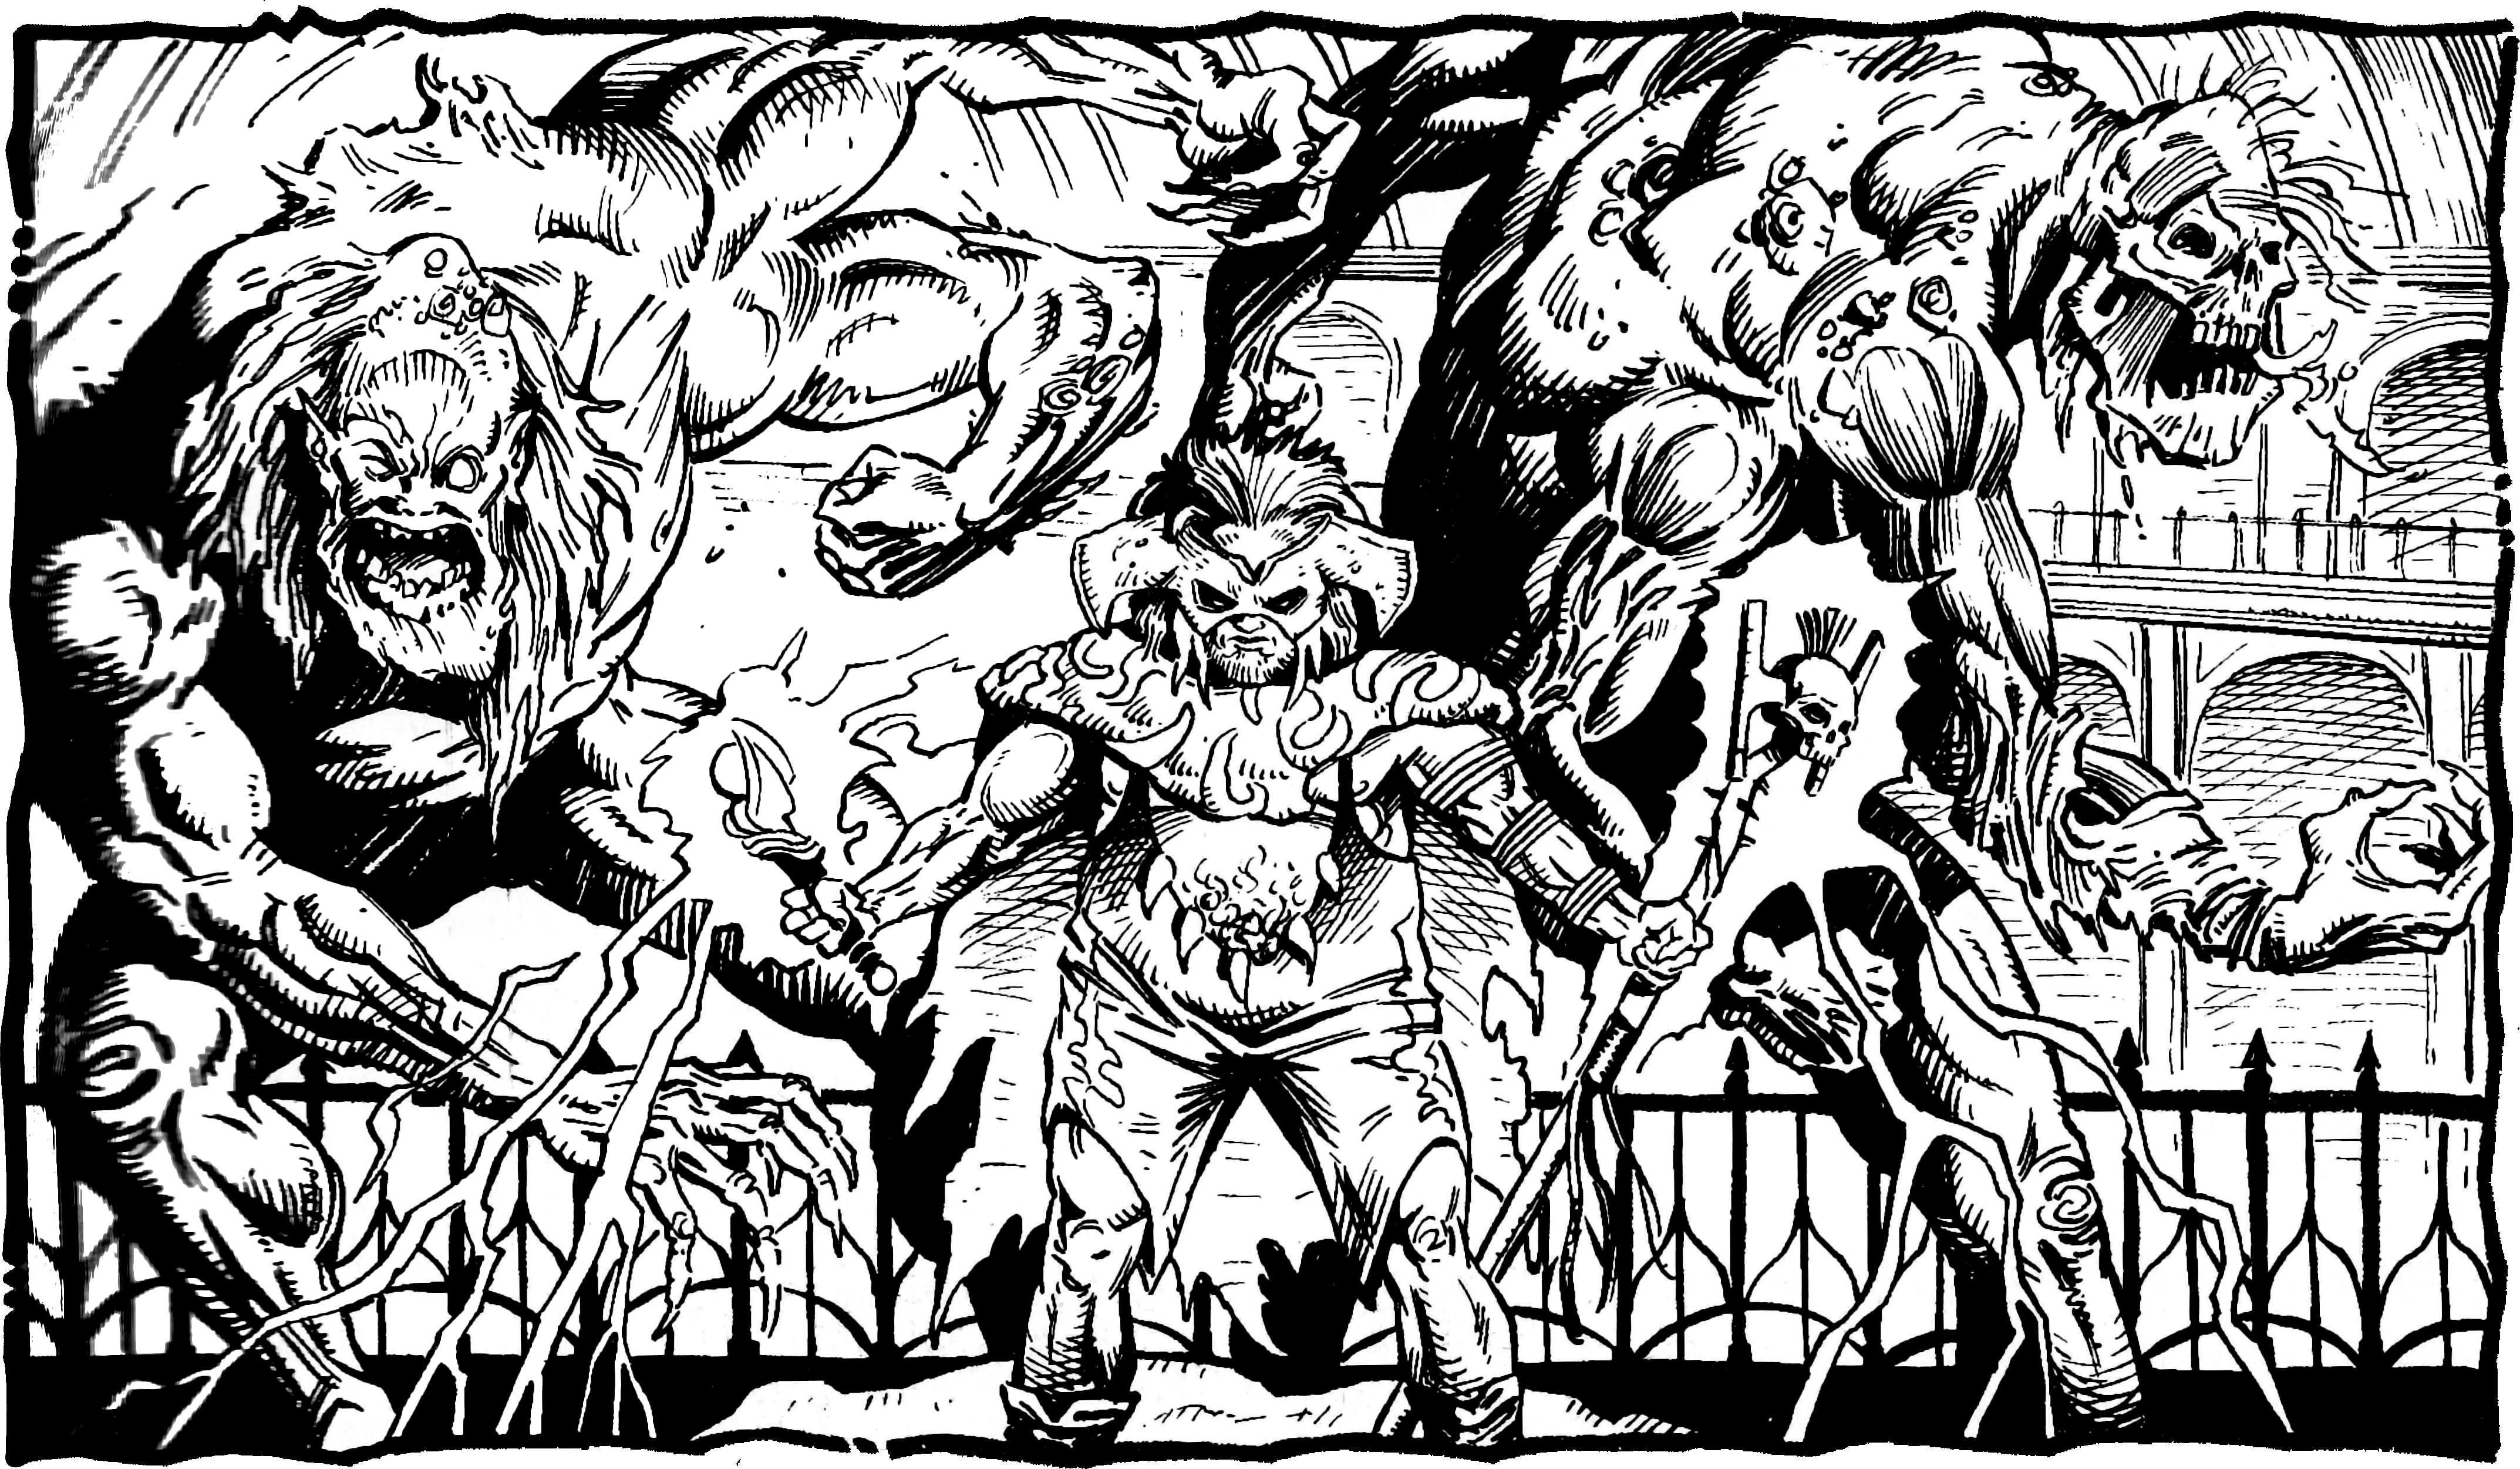
\includegraphics[width=\textwidth]{images/necromancer-1.png}
\WOTC
\end{figure*}
\AlternateClassFeature{Phantasmal Guardian}
{Halfling protectors are masters of illusions that can aid their tribes and bring doom to their enemies in many strange ways.}
{Halfling, \skill{Knowledge} (nature) 10 ranks, \skill{Spellcraft} 10 ranks.}
{10th.}
{To select this class feature, you must permanently sacrifice one of your 5th-level spell slots.}
{
	You can summon a non-corporeal shadow figure that wards an area with a radius of 30 m + 3 m per level. Any other creature entering the warded area, except you and those you designate, will be attacked by the \emph{phantasmal guardian}, as per the \spell{phantasmal killer} spell. The \emph{guardian} can only attack once, where upon it dissipates. Summoning the \emph{guardian} takes 1 minute, and it remains in the area until you dispels it (move action, unlimited range), or until it attacks someone. You can only have one \emph{guardian} summoned at a time.

	You can use this ability 3 times per day.

	\emph{Phantasmal guardian} is a spell-like ability.
}
\AlternateClassFeature{Psionic Mimicry}
{The arena mage is a wizard who has acquired the skills necessary to survive the rigors of arena combat, engaging his opponents with an arsenal of spells. The lesson to conceal this spellcasting ability comes quickly, as failure means death. As such, an arena mage becomes a
master at casting spells in secret, as well as masking his magic-use. To accomplish this feat, the arena mage has developed a unique talent to help him: giving his spells the trappings of psionic powers. Through the art of deception and a constant charade of psionic aptitude he is able to maintain secret his spellcasting even in the most public of places.}
{\skill{Bluff} 4 ranks, \skill{Concentration} 4 ranks, \skill{Disguise} 4 ranks, \skill{Knowledge} (psionics) 4 ranks.}
{1st.}
{You do not gain a familiar.}
{
	% You may attempt to conceal the fact that you are attempting to cast a spell. This is an especially important skill for wizards, who are all-too-frequently the unfortunate target of impromptu lynch mobs.
	When fighting in an gladiatorial arena, you may disguise your spells as psionic powers by making a \skill{Bluff} check as a move action, to distract the crowd. Spells with psionic counterparts, such as \spell{daze}, emulate the displays of their counterparts. Spells without psionic counterparts get attributed random displays.

	Onlookers may oppose the roll with a \skill{Sense Motive} or \skill{Spellcraft} check. If the spell being cast has a psionic counterpart, they may also oppose with a \skill{Psicraft} check.

	Defilers with this ability are accustomed to minimizing their damage in an arena and do not suffer additional penalties.
}
\AlternateClassFeature{Rebuke Undead}
{Necromants are wizards draw their power from the undead plane known as the Gray, instead of the plant life. They are seeking to unravel the mysteries of death and find answers to questions that only the ancient dead know.}
{You must be a specialist necromancer, \skill{Knowledge} (arcana) 6 ranks, \skill{Knowledge} (religion) 6 ranks.}
{5th.}
{You do not gain a bonus feat.}
{
	You gain the supernatural ability to rebuke undead. You may use this ability a number of times per day equal to 3 + your Charisma modifier. You rebuke undead as a cleric four levels lower would.
}
\Chapter{Skills}
{You can learn much from observing another being. The way the gith hunches before it leaps at you, or how the aarakocra circles before it dives. The way the halfling inhales and pauses briefly before shooting his poisoned needles, or how the Urikite trader licks his lips before making his final offer. But appearances can deceive. No two creatures are alike. Remember that when the gith hunches before casting a defiler spell, or the Urikite trader moistens his lips and spits a needle at you.}{The Oracle, Blue Shrine Scrolls}
\section{Skill Summary}
\Capitalize{I}{f} you buy a class skill, your character gets 1 rank (equal to a +1 bonus on checks with that skill) for each skill point. If you buy other classes' skills (cross-class skills), you get \onehalf rank per skill point.

Your maximum rank in a class skill is your character level + 3.

Your maximum rank in a cross-class skill is one-half of this number (do not round up or down).

\subsection{Using Skills}
To make a skill check, roll:

{
	\centering
	\vskip1em
	{\Large 1d20 + \textit{skill modifier}}
	\vskip.3em
	\Cell{\small\textit{Skill modifier} = skill rank + ability modifier\\\small + miscellaneous modifiers.}
	\vskip1em
}

This roll works just like an attack roll or a saving throw---the higher the roll, the better. Either you're trying to match or exceed a certain Difficulty Class (DC), or you're trying to beat another character's check result.

\textbf{Skill Ranks:} A character's number of ranks in a skill is based on how many skill points a character has invested in a skill. Many skills can be used even if the character has no ranks in them; doing this is called making an untrained skill check.

\textbf{Ability Modifier:} The ability modifier used in a skill check is the modifier for the skill's key ability (the ability associated with the skill's use). The key ability of each skill is noted in its description.

\textbf{Miscellaneous Modifiers:} Miscellaneous modifiers include racial bonuses, armor check penalties, and bonuses provided by feats, among others.

\subsection{Acquiring Skill Ranks}
Each skill point you spend on a class skill gets you 1 rank in that skill. Class skills are the skills found on your character's class skill list. Each skill point you spend on a cross-class skill gets your character \onehalf rank in that skill. Cross-class skills are skills not found on your character's class skill list. (Half ranks do not improve your skill check, but two \onehalf ranks make 1 rank.) You can't save skill points to spend later.

The maximum rank in a class skill is the character's level + 3. If it's a cross-class skill, the maximum rank is half of that number (do not round up or down).

Regardless of whether a skill is purchased as a class skill or a cross-class skill, if it is a class skill for any of your classes, your maximum rank equals your total character level + 3.

\section{Using Skills}
When your character uses a skill, you make a skill check to see how well he or she does. The higher the result of the skill check, the better. Based on the circumstances, your result must match or beat a particular number (a DC or the result of an opposed skill check) for the check to be successful. The harder the task, the higher the number you need to roll.

Circumstances can affect your check. A character who is free to work without distractions can make a careful attempt and avoid simple mistakes. A character who has lots of time can try over and over again, thereby assuring the best outcome. If others help, the character may succeed where otherwise he or she would fail.

\subsection{Skill Checks}
A skill check takes into account a character's training (skill rank), natural talent (ability modifier), and luck (the die roll). It may also take into account his or her race's knack for doing certain things (racial bonus) or what armor he or she is wearing (armor check penalty), or a certain feat the character possesses, among other things.

To make a skill check, roll 1d20 and add your character's skill modifier for that skill. The skill modifier incorporates the character's ranks in that skill and the ability modifier for that skill's key ability, plus any other miscellaneous modifiers that may apply, including racial bonuses and armor check penalties. The higher the result, the better. Unlike with attack rolls and saving throws, a natural roll of 20 on the d20 is not an automatic success, and a natural roll of 1 is not an automatic failure.

\subsubsection{Difficulty Class}
Some checks are made against a Difficulty Class (DC). The DC is a number (set using the skill rules as a guideline) that you must score as a result on your skill check in order to succeed.

\Table{Difficulty Class Examples}{l X}{
\tableheader Difficulty (DC) & \tableheader Example (Skill Used)\\
Very easy (0) & Notice something large in plain sight (Spot)\\
Easy (5) & Climb a knotted rope (Climb)\\
Average (10) & Hear an approaching guard (Listen)\\
Tough (15) & Rig a wagon wheel to fall off (Disable Device)\\
Challenging (20) & Swim in stormy water (Swim)\\
Formidable (25) & Open an average lock (Open Lock)\\
Heroic (30) & Leap across a 9-meter chasm (Jump)\\
Nearly impossible (40) & Track a squad of orcs across hard ground after 24 hours of rainfall (Survival)
}

\subsubsection{Opposed Checks}
An opposed check is a check whose success or failure is determined by comparing the check result to another character's check result. In an opposed check, the higher result succeeds, while the lower result fails. In case of a tie, the higher skill modifier wins. If these scores are the same, roll again to break the tie.

\Table{Example Opposed Checks}{L b{2.67cm} y{2.5cm}}{
\tableheader Task & \tableheader Skill (Key Ability) & \tableheader Opposing Skill \quad\quad (Key Ability)\\
Con someone & Bluff (Cha) & Sense Motive (Wis)\\
Pretend to be someone else & Disguise (Cha) & Spot (Wis)\\
Create a false map & Forgery (Int) & Forgery (Int)\\
Hide from someone & Hide (Dex) & Spot (Wis)\\
Sneak up on someone & Move Silently (Dex) & Listen (Wis)\\
Steal a coin pouch & Sleight of Hand (Dex) & Spot (Wis)\\
Tie a prisoner securely & Use Rope (Dex) & Escape Artist (Dex)
}

\subsubsection{Trying Again}
In general, you can try a skill check again if you fail, and you can keep trying indefinitely. Some skills, however, have consequences of failure that must be taken into account. A few skills are virtually useless once a check has failed on an attempt to accomplish a particular task. For most skills, when a character has succeeded once at a given task, additional successes are meaningless.

\subsubsection{Untrained Skill Checks}
Generally, if your character attempts to use a skill he or she does not possess, you make a skill check as normal. The skill modifier doesn't have a skill rank added in because the character has no ranks in the skill. Any other applicable modifiers, such as the modifier for the skill's key ability, are applied to the check.

Many skills can be used only by someone who is trained in them.

\subsubsection{Favorable And Unfavorable Conditions}
Some situations may make a skill easier or harder to use, resulting in a bonus or penalty to the skill modifier for a skill check or a change to the DC of the skill check.

\Table{Favorable and Unfavorable Conditions}{Lc}{
\tableheader Circumstance & \tableheader Effect in skill check \\
1 condition that improves performance         & +2 circumstance bonus \\
2 or more conditions that improve performance & Advantage \\
1 condition that hampers performance          & $-2$ penalty \\
2 or more conditions that hamper performance  & Disadvantage \\
1 condition that make the task easier         & $-2$ DC\footnotemark[1] \\
1 condition that make the task harder         & +2 DC\footnotemark[1] \\

\TableNote{2}{1 These effects are cumulative for each different condition applicable.}\\
}

The chance of success can be altered in four ways to take into account exceptional circumstances.

\begin{enumerate*}
\item Give the skill user +2 circumstance bonus on the skill check to represent conditions that improve performance, such as having the perfect tool for the job, getting help from another character (see Combining Skill Attempts), or possessing unusually accurate information. If multiple conditions apply to the situation, give the skill user advantage on the skill check, no matter how many conditions apply.
\item Give the skill user $-2$ circumstance bonus on the skill check to represent conditions that hamper performance, such as being forced to use improvised tools or having misleading information. If multiple conditions apply to the situation, give the skill user disadvantage on the skill check, no matter how many conditions apply.
\item Reduce the DC by 2 to represent circumstances that make the task easier, such as having a friendly audience or doing work that can be subpar.
\item Increase the DC by 2 to represent circumstances that make the task harder, such as having an uncooperative audience or doing work that must be flawless.
\end{enumerate*}
Conditions that affect your character's ability to perform the skill change the skill modifier. Conditions that modify how well the character has to perform the skill to succeed change the DC. A bonus to the skill modifier and a reduction in the check's DC have the same result: They create a better chance of success. But they represent different circumstances, and sometimes that difference is important.

\subsubsection{Time And Skill Checks}
Using a skill might take a round, take no time, or take several rounds or even longer. Most skill uses are standard actions, move actions, or full-round actions. Types of actions define how long activities take to perform within the framework of a combat round (6 seconds) and how movement is treated with respect to the activity. Some skill checks are instant and represent reactions to an event, or are included as part of an action.

These skill checks are not actions. Other skill checks represent part of movement.

\subsubsection{Checks Without Rolls}
A skill check represents an attempt to accomplish some goal, usually while under some sort of time pressure or distraction. Sometimes, though, a character can use a skill under more favorable conditions and eliminate the luck factor.

\textbf{Taking 10:} When your character is not being threatened or distracted, you may choose to take 10. Instead of rolling 1d20 for the skill check, calculate your result as if you had rolled a 10. For many routine tasks, taking 10 makes them automatically successful. Distractions or threats (such as combat) make it impossible for a character to take 10. In most cases, taking 10 is purely a safety measure---you know (or expect) that an average roll will succeed but fear that a poor roll might fail, so you elect to settle for the average roll (a 10). Taking 10 is especially useful in situations where a particularly high roll wouldn't help.

\textit{Taking 10 with Advantage or Disadvantage:} Consider one of the dice as 10, roll the second die. Use the higher value if you have advantage, and use the lower value if you have disadvantage. For example, if you have disadvantage and roll a 17, you use the 10. If you instead have advantage, you use the 17.

\textbf{Taking 20:} When you have plenty of time (generally 2 minutes for a skill that can normally be checked in 1 round, one full-round action, or one standard action), you are faced with no threats or distractions, and the skill being attempted carries no penalties for failure, you can take 20. In other words, eventually you will get a 20 on 1d20 if you roll enough times. Instead of rolling 1d20 for the skill check, just calculate your result as if you had rolled a 20.

Taking 20 means you are trying until you get it right, and it assumes that you fail many times before succeeding. Taking 20 takes twenty times as long as making a single check would take.

Since taking 20 assumes that the character will fail many times before succeeding, if you did attempt to take 20 on a skill that carries penalties for failure, your character would automatically incur those penalties before he or she could complete the task. Common ``take 20'' skills include \skill{Escape Artist}, \skill{Open Lock}, and \skill{Search}.

\textbf{Ability Checks and Caster Level Checks:} The normal take 10 and take 20 rules apply for ability checks. Neither rule applies to caster level checks.

\subsection{Combining Skill Attempts}
When more than one character tries the same skill at the same time and for the same purpose, their efforts may overlap.

\subsubsection{Individual Events}
Often, several characters attempt some action and each succeeds or fails independently. The result of one character's \skill{Climb} check does not influence the results of other characters \skill{Climb} check.

\subsubsection{Aid Another}
You can help another character achieve success on his or her skill check by making the same kind of skill check in a cooperative effort. If you roll a 10 or higher on your check, the character you are helping gets advantage on his or her check, as per the rule for favorable conditions. (You can't take 10 on a skill check to aid another.) In many cases, a character's help won't be beneficial, or only a limited number of characters can help at once.

In cases where the skill restricts who can achieve certain results you can't aid another to grant a bonus to a task that your character couldn't achieve alone.

\subsubsection{Skill Synergy}
It's possible for a character to have two skills that work well together. In general, having 5 or more ranks in one skill gives the character a +2 bonus on skill checks with each of its synergistic skills, as noted in the skill description. In some cases, this bonus applies only to specific uses of the skill in question, and not to all checks. Some skills provide benefits on other checks made by a character, such as those checks required to use certain class features.

\Table{Skill Synergies}{L p{4.9cm}}{
\tableheader 5 or more ranks in... & \tableheader Gives a +2 bonus on...\\
Appraise & Diplomacy checks to bargain\\
Autohypnosis & Knowledge (psionics) checks\\
Balance & Tumble checks\\
Bluff & Diplomacy checks\\
Bluff & Disguise checks to act in character\\
Bluff & Intimidate checks\\
Bluff & Sleight Of Hand checks\\
Concentration & Autohypnosis checks\\
Craft & related Appraise checks\\
Decipher Script & Forgery checks\\
Decipher Script & Use Magic Device checks involving scrolls\\
Diplomacy & Gather Information checks\\
Disable Device & Open Lock checks\\
Escape Artist & Use Rope checks involving bindings\\
Handle Animal & Ride checks\\
Handle Animal & wild empathy checks\\
Jump & Tumble checks\\
Knowledge (arcana) & Spellcraft checks\\
~ (architecture and engineering) & Search checks involving secret doors and similar compartments\\
~ (dungeoneering) & Survival checks when underground\\
~ (geography) & Survival checks to keep from getting lost or for avoiding hazards\\
~ (history) & bardic knowledge checks\\
~ (local) & Gather Information checks\\
~ (nature) & Survival checks in aboveground natural environments\\
~ (nobility and royalty) & Diplomacy checks\\
~ (psionics) & Psicraft checks\\
~ (religion) & checks to turn or rebuke undead\\
~ (the planes) & Survival checks when on other planes\\
~ (warcraft) & Diplomacy checks dealing with troops\\
Open Lock & Disable Device checks\\
% Psicraft & Use Psionic Device checks involving power stones\\
Ride & Handle Animal checks involving mounts\\
Search & Survival checks when following tracks\\
Sense Motive & Diplomacy checks\\
Spellcraft & Use Magic Device involving scrolls\\
Survival & Knowledge (nature) checks\\
Tumble & Balance checks\\
Tumble & Jump checks\\
Use Magic Device & Appraise checks involving magic items\\
Use Magic Device & Spellcraft checks to decipher scrolls\\
Use Psionic Device & Appraise checks involving psionic items\\
% Use Psionic Device & Psicraft checks to address power stones\\
Use Rope & Climb checks involving climbing ropes\\
Use Rope & Escape Artist checks involving ropes
}

\subsection{Ability Checks}
Sometimes a character tries to do something to which no specific skill really applies. In these cases, you make an ability check. An ability check is a roll of 1d20 plus the appropriate ability modifier. Essentially, you're making an untrained skill check.

In some cases, an action is a straight test of one's ability with no luck involved. Just as you wouldn't make a height check to see who is taller, you don't make a Strength check to see who is stronger.

\section{Skill Descriptions}
This section describes each skill, including common uses and typical modifiers. Characters can sometimes use skills for purposes other than those noted here.

Here is the format for skill descriptions.

\subsection{Skill Name}
The skill name line includes (in addition to the name of the skill) the following information.

\textbf{Key Ability:} The abbreviation of the ability whose modifier applies to the skill check. Exception: \skill{Speak Language} and \skill{Literacy} have ``None'' as its key ability because the use of those skills does not require a check.

\textbf{Trained Only:} If this notation is included in the skill name line, you must have at least 1 rank in the skill to use it. If it is omitted, the skill can be used untrained (with a rank of 0). If any special notes apply to trained or untrained use, they are covered in the Untrained section (see below).

\textbf{Armor Check Penalty:} If this notation is included in the skill name line, an armor check penalty applies (when appropriate) to checks using this skill. If this entry is absent, an armor check penalty does not apply.

The skill name line is followed by a general description of what using the skill represents. After the description are a few other types of information:

\textbf{Check:} What a character (``you'' in the skill description) can do with a successful skill check and the check's DC.

\textbf{Action:} The type of action using the skill requires, or the amount of time required for a check.

\textbf{Try Again:} Any conditions that apply to successive attempts to use the skill successfully. If the skill doesn't allow you to attempt the same task more than once, or if failure carries an inherent penalty (such as with the Climb skill), you can't take 20. If this paragraph is omitted, the skill can be retried without any inherent penalty, other than the additional time required.

\textbf{Special:} Any extra facts that apply to the skill, such as special effects deriving from its use or bonuses that certain characters receive because of class, feat choices, or race.

\textbf{Synergy:} Some skills grant a bonus to the use of one or more other skills because of a synergistic effect. This entry, when present, indicates what bonuses this skill may grant or receive because of such synergies. See \tabref{Skill Synergies} for a complete list of bonuses granted by synergy between skills (or between a skill and a class feature).

\textbf{Restriction:} The full utility of certain skills is restricted to characters of certain classes or characters who possess certain feats. This entry indicates whether any such restrictions exist for the skill.

\textbf{Untrained:} This entry indicates what a character without at least 1 rank in the skill can do with it. If this entry doesn't appear, it means that the skill functions normally for untrained characters (if it can be used untrained) or that an untrained character can't attempt checks with this skill (for skills that are designated as ``Trained Only'').

\Figure{b}{images/artifact-2.png}
\Skill{Appraise}{Int}
\textbf{Check:} You can appraise common or well-known objects with a DC 12 Appraise check. Failure means that you estimate the value at 50\% to 150\% (2d6+3 times 10\%,) of its actual value.

Appraising a rare or exotic item requires a successful check against DC 15, 20, or higher. If the check is successful, you estimate the value correctly; failure means you cannot estimate the item's value.

\Table{Appraise DCs}{L c}{
\tableheader Type (Examples) & \tableheader Appraise DC \\

Common items (Trade goods, mundane items) & 12\footnotemark[1] \\
Rare items (Fine clothing, precious metals, gems, artwork) & 15\footnotemark[2] \\
Exotic items (Jewelry, spell components, obscure religous items) & 20\footnotemark[2] \\
Unique items (Masterwork artwork, royal adornment) & 25\footnotemark[2] \\
Magical items\footnotemark[3] & 15 + caster level \\
Psionic items\footnotemark[3] & 10 + manifester level \\

\TableNote{2}{1 Failure means that you estimate the value at 2d6+3 $\times$ 10\% of its actual value.}\\
\TableNote{2}{2 Failure means you cannot estimate the item's value.}\\
\TableNote{2}{3 Requires a special ritual to assess the items properties.}\\
}

A magnifying glass gives you +2 circumstance bonus on Appraise checks involving any item that is small or highly detailed, such as a gem. A merchant's scale gives you +2 circumstance bonus on Appraise checks involving any items that are valued by weight, including anything made of precious metals.

Using both items give advantage on the check, instead.

\textit{Appraise Item of Power:} If you know that an item is magical or psionic, you can use Appraise to identify the item's properties. This use requires 25 cp worth of special materials. The DC for appraising magical items is 15 + the caster level of the item, and the DC for psionic items is 10 + the manifester level of the item.

\textbf{Action:} Appraising a mundane item takes 1 minute (ten consecutive full-round actions). Appraising a magical or psionic item takes 8 hours of uninterrupted work.

\textbf{Try Again:} No. You cannot try again on the same object, regardless of success.

\textbf{Special:} The master of a raven familiar gains a +3 bonus on Appraise checks.

A character with the \feat{Diligent} feat or the \feat{Trader} feat gets a +2 bonus on Appraise checks.

\textbf{Synergy:} If you have 5 ranks in Appraise, you gain a +2 bonus on \skill{Diplomacy} checks related to bargaining.

If you have 5 ranks in any \skill{Craft} skill, you gain a +2 bonus on Appraise checks related to items made with that \skill{Craft} skill.

\textbf{Untrained:} For common items, failure on an untrained check means no estimate. For rare items, success means an estimate of 50\% to 150\% (2d6+3 times 10\%). You can't appraise magical or psionic items with an untrained check.
\Figure*{b}{images/gladiator-5.png}
\Skill{Autohypnosis}{wis; trained only}
You have trained your mind to gain mastery over your body and the mind's own deepest capabilities.

\textbf{Check:} The DC and the effect of a successful check depend on the task you attempt.

\Table{Autohypnosis DCs}{X R}{
\tableheader Task & \tableheader DC\\
Ignore caltrop wound & 18\\
Memorize             & 15\\
Rejuvenate           & 20\\
Resist dying         & 20\\
Resist fear          & Fear effect DC\\
Tolerate poison      & Poison's DC\\
Willpower            & 20\\
}

\textit{Ignore Caltrop Wound:} If you are wounded by stepping on a caltrop, your speed is reduced to one-half normal. A successful Autohypnosis check removes this movement penalty. The wound doesn't go away---it is just ignored through self-persuasion.

\textit{Memorize:} You can attempt to memorize a long string of numbers, a long passage of verse, or some other particularly difficult piece of information (but you can't memorize magical writing or similarly exotic scripts). Each successful check allows you to memorize a single page of text (up to 800 words), numbers, diagrams, or sigils (even if you don't recognize their meaning). If a document is longer than one page, you can make additional checks for each additional page. You always retain this information; however, you can recall it only with another successful Autohypnosis check.

\textit{Rejuvenate:} You enter in a deep state of meditation, and recover power points as quickly as if you were sleeping. You continue this state until you choose to finish willingly.

\textit{Resist Dying:} You can attempt to subconsciously prevent yourself from dying. If you have negative hit points and are losing hit points (at 1 per round, 1 per hour), you can substitute a DC 20 Autohypnosis check for your d\% roll to see if you become stable. If the check is successful, you stop losing hit points (you do not gain any hit points, however, as a result of the check). You can substitute this check for the d\% roll in later rounds if you are initially unsuccessful.

\textit{Resist Fear:} In response to any fear effect, you make a saving throw normally. If you fail the saving throw, you can make an Autohypnosis check on your next round even while overcome by fear. If your Autohypnosis check meets or beats the DC for the fear effect, you shrug off the fear. On a failed check, the fear affects you normally, and you gain no further attempts to shrug off that particular fear effect.

\textit{Tolerate Poison:} You can choose to substitute an Autohypnosis check for a saving throw against any standard poison's secondary damage or effect. This skill has no effect on the initial saving throw against poison.

\textit{Willpower:} If reduced to 0 hit points (disabled), you can make an Autohypnosis check. If successful, you can take a normal action while at 0 hit points without taking 1 point of damage. You must make a check for each strenuous action you want to take. A failed Autohypnosis check in this circumstance carries no direct penalty---you can choose not to take the strenuous action and thus avoid the hit point loss. If you do so anyway, you drop to $-1$ hit points, as normal when disabled.

\textbf{Action:} None. Making an Autohypnosis check doesn't require an action; it is either a free action (when attempted reactively) or part of another action (when attempted actively).

\textbf{Try Again:} Yes, for memorize and willpower uses, though a success doesn't cancel the effects of a previous failure. No for the other uses.

\textbf{Special:} If you have the \feat{Autonomous} feat, you get a +2 bonus on Autohypnosis checks.
\Figure*{b}{images/bluff.png}
\Skill{Balance}{dex; armor check penalty}
\textbf{Check:} You can walk on a precarious surface. A successful check lets you move at half your speed along the surface for 1 round. A failure by 4 or less means you can't move for 1 round. A failure by 5 or more means you fall. The difficulty varies with the surface, as follows:

\Table{Balance DCs}{X Z{9mm} X Z{9mm}}{
  \tableheader Narrow Surface
& \tableheader Balance DC
& \tableheader Difficult Surface
& \tableheader Balance DC\\
15--30 cm wide      & 10 & Uneven flagstone       & 10\\
5--14 cm wide       & 15 & Hewn stone floor       & 10\\
2--5 cm wide        & 20 & Sloped or angled floor & 10\\
Less than 2 cm wide & 40 &&\\
}

\Table{Narrow Surface Modifiers}{X c}{
  \tableheader Surface
& \tableheader DC Modifier \\
Lightly obstructed  & +2 \\
Severely obstructed & +5 \\
Lightly slippery    & +2 \\
Severely slippery   & +5 \\
Sloped or angled    & +2 \\
}

For narrow surfaces, use the DC given on \tabref{Balance DCs} and add modifiers from \tabref{Narrow Surface Modifiers}, as appropriate. Those modifiers stack.

Make checks for difficult surfaces only if running or charging. Failure by 4 or less means the character can't run or charge, but may otherwise act normally.

\textit{Being Attacked while Balancing:} You are considered flat-footed while balancing, since you can't move to avoid a blow, and thus you lose your Dexterity bonus to AC (if any). If you have 10 or more ranks in Balance, you aren't considered flat-footed while balancing. If you take damage while balancing, you must make another Balance check against the same DC to remain standing.

\textit{Accelerated Movement:} You can try to walk across a precarious surface more quickly than normal. If you accept a $-5$ penalty, you can move your full speed as a move action. (Moving twice your speed in a round requires two Balance checks, one for each move action used.) You may also accept this penalty in order to charge across a precarious surface; charging requires one Balance check for each multiple of your speed (or fraction thereof) that you charge.

\textit{Sprinting Balance:} You can try to run across a narrow surface by accepting a $-20$ penalty on your Balance check.

\textbf{Action:} None. A Balance check doesn't require an action; it is made as part of another action or as a reaction to a situation.

\textbf{Special:} If you have the \feat{Agile} feat, you get a +2 bonus on Balance checks.

If you have 10 or more ranks in Balance, you can make a Balance check in place of a Strength or Dexterity check to avoid being tripped by an opponent. You take a $-10$ penalty on your Balance check. If you succeed on this check, you are not tripped. When you succeed on a Balance check to resist being tripped, you may not attempt to trip your opponent.

\textbf{Synergy:} If you have 5 or more ranks in \skill{Tumble}, you get a +2 bonus on Balance checks.

If you have 5 or more ranks in Balance, you get a +2 bonus on \skill{Tumble} checks.
\Skill{Bluff}{cha}
\textbf{Check:} A Bluff check is opposed by the target's Sense Motive check. See the accompanying table for examples of different kinds of bluffs and the modifier to the target's Sense Motive check for each one.

Favorable and unfavorable circumstances weigh heavily on the outcome of a bluff. Two circumstances can weigh against you: The bluff is hard to believe, or the action that the target is asked to take goes against its self-interest, nature, personality, orders, or the like. If it's important, you can distinguish between a bluff that fails because the target doesn't believe it and one that fails because it just asks too much of the target. For instance, if the target gets a +10 bonus on its Sense Motive check because the bluff demands something risky, and the Sense Motive check succeeds by 10 or less, then the target didn't so much see through the bluff as prove reluctant to go along with it. A target that succeeds by 11 or more has seen through the bluff.

A successful Bluff check indicates that the target reacts as you wish, at least for a short time (usually 1 round or less) or believes something that you want it to believe. Bluff, however, is not a suggestion spell.

A bluff requires interaction between you and the target. Creatures unaware of you cannot be bluffed.

\Table{Bluff Examples}{X r{1.5cm}}{
\tableheader Example Circumstances & \tableheader Sense Motive Modifier\\
The target wants to believe you. & $-5$\\
The bluff is believable and doesn't affect the target much. & +0\\
The bluff is a little hard to believe or puts the target at some risk. & +5\\
The bluff is hard to believe or puts the target at significant risk. & +10\\
The bluff is way out there, almost too incredible to consider. & +20
}

\textit{Feinting in Combat:} You can also use Bluff to mislead an opponent in melee combat (so that it can't dodge your next attack effectively). To feint, make a Bluff check opposed by your target's Sense Motive check, but in this case, the target may add its base attack bonus to the roll along with any other applicable modifiers.

If your Bluff check result exceeds this special Sense Motive check result, your target is denied its Dexterity bonus to AC (if any) for the next melee attack you make against it. This attack must be made on or before your next turn.

Feinting in this way against a nonhumanoid is difficult because it's harder to read a strange creature's body language; you take a $-4$ penalty on your Bluff check. Against a creature of animal Intelligence (1 or 2) it's even harder; you take a $-8$ penalty. Against a nonintelligent creature, it's impossible.

Feinting in combat does not provoke an attack of opportunity.

\textit{Creating a Diversion to Hide:} You can use the Bluff skill to help you hide. A successful Bluff check gives you the momentary diversion you need to attempt a Hide check while people are aware of you. This usage does not provoke an attack of opportunity.

\textit{Delivering a Secret Message:} You can use Bluff to get a message across to another character without others understanding it. The DC is 15 for simple messages, or 20 for complex messages, especially those that rely on getting across new information. Failure by 4 or less means you can't get the message across. Failure by 5 or more means that some false information has been implied or inferred. Anyone listening to the exchange can make a Sense Motive check opposed by the Bluff check you made to transmit in order to intercept your message (see Sense Motive).

% \textit{Conceal Spellcasting:} Spellcasters may attempt to conceal the fact that they are attempting to cast a spell. This is an especially important skill for wizards, who are all-too-frequently the unfortunate target of impromptu lynch mobs. When casting a spell, a spellcaster may attempt to conceal verbal and somatic components by making a Bluff check as a move action, to distract any witnesses. Onlookers may oppose the roll with a Sense Motive or Spellcraft check.

% Attempting to conceal spellcasting if the spellcaster is defiling carries a $-20$ circumstance penalty.
% % Bluff
% % The spellcaster is defiling & $-20$
% % Spellcraft or Sense Motive

% \Table{}{X r{2cm}}{
% \tableheader Circumstances & \tableheader Spellcraft/Sense Motive Modifier\\
% Target is closely observing spellcaster & +5\\
% Target knows the character is a spellcaster & +5
% }

% Casting spells in cities with witnesses can be very dangerous. Lynch mobs, templars and even other wizards generally flock to the scene when someone cries \textit{``Wizard!''}.

\textbf{Action:} Varies. A Bluff check made as part of general interaction always takes at least 1 round (and is at least a full-round action), but it can take much longer if you try something elaborate. A Bluff check made to feint in combat or create a diversion to hide is a standard action. A Bluff check made to conceal spellcasting is a move action. A Bluff check made to deliver a secret message doesn't take an action; it is part of normal communication.

\textbf{Try Again:} Varies. Generally, a failed Bluff check in social interaction makes the target too suspicious for you to try again in the same circumstances, but you may retry freely on Bluff checks made to feint in combat. Retries are also allowed when you are trying to send a message, but you may attempt such a retry only once per round.

Each retry carries the same chance of miscommunication.

\textbf{Special:} A ranger gains a bonus on Bluff checks when using this skill against a favored enemy.

The master of a snake familiar gains a +3 bonus on Bluff checks.

If you have the \feat{Persuasive} feat or the \feat{Trader} feat, you get a +2 bonus on Bluff checks.

\textbf{Synergy:} If you have 5 or more ranks in Bluff, you get a +2 bonus on \skill{Diplomacy}, \skill{Intimidate}, and \skill{Sleight of Hand} checks, as well as on \skill{Disguise} checks made when you know you're being observed and you try to act in character.


\Skill{Climb}{Str; Armor Check Penalty}
\textbf{Check:} With a successful Climb check, you can advance up, down, or across a slope, a wall, or some other steep incline (or even a ceiling with handholds) at one-quarter your normal speed. A slope is considered to be any incline at an angle measuring less than 60 degrees; a wall is any incline at an angle measuring 60 degrees or more.

A Climb check that fails by 4 or less means that you make no progress, and one that fails by 5 or more means that you fall from whatever height you have already attained.

A climber's kit gives you advantage on Climb checks.

The DC of the check depends on the conditions of the climb. Compare the task with those on the following table to determine an appropriate DC.

\Table{Climb DCs}{l X}{
\tableheader Climb DC & \tableheader Example Surface or Activity\\
0 & A slope too steep to walk up, or a knotted rope with a wall to brace against.\\
5 & A rope with a wall to brace against, or a knotted rope, or a rope affected by the rope trick spell.\\
10 & A surface with ledges to hold on to and stand on, such as a very rough wall or a ship's rigging.\\
15 & Any surface with adequate handholds and footholds (natural or artificial), such as a very rough natural rock surface or a tree, or an unknotted rope, or pulling yourself up when dangling by your hands.\\
20 & An uneven surface with some narrow handholds and footholds, such as a typical wall in a dungeon or ruins.\\
25 & A rough surface, such as a natural rock wall or a brick wall.\\
25 & An overhang or ceiling with handholds but no footholds.\\
--- & A perfectly smooth, flat, vertical surface cannot be climbed.
}

\Table{Climb DC Modifiers}{l X}{
\tableheader Climb DC Modifier & Example Surface or Activity\\
% These modifiers are cumulative; use any that apply.
$-10$ & Climbing a chimney (artificial or natural) or other location where you can brace against two opposite walls (reduces DC by 10).\\
-5 & Climbing a corner where you can brace against perpendicular walls (reduces DC by 5).\\
+5 & Surface is slippery (increases DC by 5).
}

You need both hands free to climb, but you may cling to a wall with one hand while you cast a spell or take some other action that requires only one hand. While climbing, you can't move to avoid a blow, so you lose your Dexterity bonus to AC (if any). You also can't use a shield while climbing.

Any time you take damage while climbing, make a Climb check against the DC of the slope or wall. Failure means you fall from your current height and sustain the appropriate falling damage.

\textit{Accelerated Climbing:} You try to climb more quickly than normal. By accepting a $-5$ penalty, you can move half your speed (instead of one-quarter your speed).

\textit{Making Your Own Handholds and Footholds:} You can make your own handholds and footholds by pounding pitons into a wall. Doing so takes 1 minute per piton, and one piton is needed per meter of distance. As with any surface that offers handholds and footholds, a wall with pitons in it has a DC of 15. In the same way, a climber with a handaxe or similar implement can cut handholds in an ice wall.

\textit{Catching Yourself When Falling:} It's practically impossible to catch yourself on a wall while falling. Make a Climb check (DC = wall's DC + 20) to do so. It's much easier to catch yourself on a slope (DC = slope's DC + 10).

\textit{Catching a Falling Character While Climbing:} If someone climbing above you or adjacent to you falls, you can attempt to catch the falling character if he or she is within your reach. Doing so requires a successful melee touch attack against the falling character (though he or she can voluntarily forego any Dexterity bonus to AC if desired). If you hit, you must immediately attempt a Climb check (DC = wall's DC + 10). Success indicates that you catch the falling character, but his or her total weight, including equipment, cannot exceed your heavy load limit or you automatically fall. If you fail your Climb check by 4 or less, you fail to stop the character's fall but don't lose your grip on the wall. If you fail by 5 or more, you fail to stop the character's fall and begin falling as well.

\textbf{Action:} Climbing is part of movement, so it's generally part of a move action (and may be combined with other types of movement in a move action). Each move action that includes any climbing requires a separate Climb check. Catching yourself or another falling character doesn't take an action.

\textbf{Special:} You can use a rope to haul a character upward (or lower a character) through sheer strength. You can lift double your maximum load in this manner.

A halfling has a +2 racial bonus on Climb checks because halflings are agile and surefooted.

The master of a lizard familiar gains a +3 bonus on Climb checks.

If you have the \feat{Athletic} feat, you get a +2 bonus on Climb checks.

A creature with a climb speed has a +8 racial bonus on all Climb checks. The creature must make a Climb check to climb any wall or slope with a DC higher than 0, but it always can choose to take 10, even if rushed or threatened while climbing. If a creature with a climb speed chooses an accelerated climb (see above), it moves at double its climb speed (or at its land speed, whichever is slower) and makes a single Climb check at a $-5$ penalty. Such a creature retains its Dexterity bonus to Armor Class (if any) while climbing, and opponents get no special bonus to their attacks against it. It cannot, however, use the run action while climbing.

\textbf{Synergy:} If you have 5 or more ranks in \skill{Use Rope}, you get a +2 bonus on Climb checks made to climb a rope, a knotted rope, or a rope-and-wall combination.
\Figure{b}{images/psion-5.png}
\Skill{Concentration}{Con}
\textbf{Check:} You must make a Concentration check whenever you might potentially be distracted (by taking damage, by harsh weather, and so on) while engaged in some action that requires your full attention. Such actions include casting a spell, concentrating on an active spell, directing a spell, using a spell-like ability, or using a skill that would provoke an attack of opportunity. In general, if an action wouldn't normally provoke an attack of opportunity, you need not make a Concentration check to avoid being distracted.

If the Concentration check succeeds, you may continue with the action as normal. If the check fails, the action automatically fails and is wasted. If you were in the process of casting a spell, the spell is lost. If you were concentrating on an active spell, the spell ends as if you had ceased concentrating on it. If you were directing a spell, the direction fails but the spell remains active. If you were using a spell-like ability, that use of the ability is lost. A skill use also fails, and in some cases a failed skill check may have other ramifications as well.

The table below summarizes various types of distractions that cause you to make a Concentration check. If the distraction occurs while you are trying to cast a spell, you must add the level of the spell you are trying to cast to the appropriate Concentration DC. If more than one type of distraction is present, make a check for each one; any failed Concentration check indicates that the task is not completed.

If you are trying to cast, concentrate on, or direct a spell when the distraction occurs, add the level of the spell to the indicated DC.

If the distracting spell or power allows no save, use the save DC it would have if it did allow a save.

\Table{Concentration DCs}{Y{3cm} >{\raggedright\arraybackslash}X}{
\tableheader Concentration DC & \tableheader Distraction\\
% 
% Such as during the casting of a spell with a casting time of 1 round or more, or the execution of an activity that takes more than a single full-round action (such as Disable Device). Also, damage stemming from an attack of opportunity or readied attack made in response to the spell being cast (for spells with a casting time of 1 standard action) or the action being taken (for activities requiring no more than a full-round action).
% Such as from acid arrow.
% 
10 + damage dealt & Damaged during the action.\\
10 + half of continuous damage last dealt & Taking continuous damage during the action, such as from \emph{acid arrow}.\\
Distracting spell's save DC & Distracted by nondamaging spell.\\
10 & Vigorous motion (on a moving mount, taking a bouncy wagon ride, in a small boat in rough water, belowdecks in a stormtossed ship).\\
15 & Violent motion (on a galloping horse, taking a very rough wagon ride, in a small boat in rapids, on the deck of a storm-tossed ship).\\
20 & Extraordinarily violent motion (earthquake).\\
15 & Entangled.\\
20 & Grappling or pinned. (You can cast only spells without somatic components for which you have any required material component in hand.)\\
5 & Weather is a high wind carrying blinding rain or sleet.\\
10 & Weather is wind-driven hail, dust, or debris.\\
Distracting spell's save DC & Weather caused by a spell, such as \emph{storm of vengeance}.\\
% \hline
Distracting power's save DC & Distracted by nondamaging power.\\
15 + power level & Attempting to manifest a power without its display.\\
20 & Gain psionic focus.\\
20 & Grappling or pinned. (You can manifest powers normally unless you fail your Concentration check.)\\
Distracting power's save DC & Weather caused by power
}

\textit{Gain Psionic Focus:} Merely holding a reservoir of psionic power points in mind gives psionic characters a special energy. Psionic characters can put that energy to work without actually paying a power point cost---they can become psionically focused as a special use of the Concentration skill.

If you have 1 or more power points available, you can meditate to attempt to become psionically focused. The DC to become psionically focused is 20. Meditating is a full-round action that provokes attacks of opportunity. When you are psionically focused, you can expend your focus on any single Concentration check you make thereafter. When you expend your focus in this manner, your Concentration check is treated as if you rolled a 15. It's like taking 10, except that the number you add to your Concentration modifier is 15. You can also expend your focus to gain the benefit of a psionic feat---many psionic feats are activated in this way.

Once you are psionically focused, you remain focused until you expend your focus, become unconscious, or go to sleep (or enter a meditative trance, in the case of elans), or until your power point reserve drops to 0.

\textbf{Action:} Usually none. In most cases, making a Concentration check doesn't require an action; it is either a free action (when attempted reactively) or part of another action (when attempted actively). Meditating to gain psionic focus is a full-round action.

\textbf{Try Again:} Yes, though a success doesn't cancel the effect of a previous failure, such as the loss of a spell you were casting or the disruption of a spell you were concentrating on.

\textbf{Special:} You can use Concentration to cast a spell, use a spell-like ability, or use a skill defensively, so as to avoid attacks of opportunity altogether. This doesn't apply to other actions that might provoke attacks of opportunity.

The DC of the check is 15 (plus the spell's level, if casting a spell or using a spell-like ability defensively). If the Concentration check succeeds, you may attempt the action normally without provoking any attacks of opportunity. A successful Concentration check still doesn't allow you to take 10 on another check if you are in a stressful situation; you must make the check normally. If the Concentration check fails, the related action also automatically fails (with any appropriate ramifications), and the action is wasted, just as if your concentration had been disrupted by a distraction.

A character with the Combat Casting feat gets a +4 bonus on Concentration checks made to cast a spell or use a spell-like ability while on the defensive or while grappling or pinned.

You can use Concentration to manifest a power or use a psi-like ability defensively, so as to avoid attacks of opportunity altogether. The DC of the check is 15 + the power's level. If the Concentration check succeeds, you can manifest normally without provoking any attacks of opportunity. If the Concentration check fails, the power also automatically fails and the power points are wasted, just as if your concentration had been disrupted by a distraction.

A character with the Combat Manifestation feat gets a +4 bonus on Concentration checks made to manifest a power or use a psi-like ability while on the defensive or while grappling or pinned.

\textbf{Synergy:} If you have 5 or more ranks in Concentration, you get a +2 bonus on \skill{Autohypnosis} checks.
\Figure{b}{images/craft.png}
\Skill{Craft}{Int}
Like \skill{Knowledge}, \skill{Perform}, and \skill{Profession}, Craft is actually a number of separate skills. You could have several Craft skills, each with its own ranks, each purchased as a separate skill.

A Craft skill is specifically focused on creating something. If nothing is created by the endeavor, it probably falls under the heading of a Profession skill.

\textbf{Check:} You can practice your trade and make a decent living, earning about half your check result in gold pieces per week of dedicated work. You know how to use the tools of your trade, how to perform the craft's daily tasks, how to supervise untrained helpers, and how to handle common problems. (Untrained laborers and assistants earn an average of 1 silver piece per day.)

The basic function of the Craft skill, however, is to allow you to make an item of the appropriate type. The DC depends on the complexity of the item to be created. The DC, your check results, and the price of the item determine how long it takes to make a particular item. The item's finished price also determines the cost of raw materials.

In some cases, the fabricate spell can be used to achieve the results of a Craft check with no actual check involved. However, you must make an appropriate Craft check when using the spell to make articles requiring a high degree of craftsmanship.

A successful Craft check related to woodworking in conjunction with the casting of the ironwood spell enables you to make wooden items that have the strength of steel.

When casting the spell minor creation, you must succeed on an appropriate Craft check to make a complex item.

All crafts require artisan's tools to give the best chance of success. If improvised tools are used, the check is made with a $-2$ circumstance penalty. On the other hand, masterwork artisan's tools provide a +2 circumstance bonus on the check.

To determine how much time and money it takes to make an item, follow these steps.

\begin{enumerate*}
\item Find the item's price. Put the price in bits (1 ceramic = 10 bits).
\item Find the DC from the table below.
\item Pay one-third of the item's price for the cost of raw materials.
\item Make an appropriate Craft check representing one week's work. If the check succeeds, multiply your check result by the DC. If the result $\times$ the DC equals the price of the item in bits, then you have completed the item. (If the result $\times$ the DC equals double or triple the price of the item in bits, then you've completed the task in one-half or one-third of the time. Other multiples of the DC reduce the time in the same manner.) If the result $\times$ the DC doesn't equal the price, then it represents the progress you've made this week. Record the result and make a new Craft check for the next week. Each week, you make more progress until your total reaches the price of the item in bits.
\end{enumerate*}

Creating metal items takes 10 times longer than crafting non-metal items. It also carries a $-5$ penalty on all Craft checks.

If you fail a check by 4 or less, you make no progress this week.

If you fail by 5 or more, you ruin half the raw materials and have to pay half the original raw material cost again.

\textit{Progress by the Day:} You can make checks by the day instead of by the week. In this case your progress (check result $\times$ DC) is in lead beads instead of bits.

\textit{Creating Masterwork Items:} You can make a masterwork item---a weapon, suit of armor, shield, or tool that conveys a bonus on its use through its exceptional craftsmanship, not through being magical. To create a masterwork item, you create the masterwork component as if it were a separate item in addition to the standard item. The masterwork component has its own price (300 cp for a weapon, 300 cp for a poison, or 150 cp for a suit of armor or a shield) and a Craft DC of 20. Once both the standard component and the masterwork component are completed, the masterwork item is finished. Note: The cost you pay for the masterwork component is one-third of the given amount, just as it is for the cost in raw materials.

\textit{Repairing Items:} Generally, you can repair an item by making checks against the same DC that it took to make the item in the first place. The cost of repairing an item is one-fifth of the item's price.

When you use the Craft skill to make a particular sort of item, the DC for checks involving the creation of that item are typically as given on the following table.

\Table{Craft DCs}{L l Y{1.2cm}}{
\tableheader Item & \tableheader Craft Skill & \tableheader Craft DC\\
% You must be a spellcaster to craft any of these items.
% Traps have their own rules for construction.
Acid & Alchemy & 15\\
Alchemist's fire, smokestick, or tindertwig & Alchemy & 20\\
Antitoxin, sunrod, tanglefoot bag, or thunderstone & Alchemy & 25\\
Armor or shield & Armorsmithing & 10 + AC bonus\\
Longbow or shortbow & Bowmaking & 12\\
Composite longbow or composite shortbow & Bowmaking & 15\\
Composite longbow or composite shortbow with high strength rating & Bowmaking & 15 + (2 $\times$ rating)\\
Contact poison & Poisonmaking & 10 + save DC\\
Ingested poison & Poisonmaking & 5 + save DC\\
Inhaled poison & Poisonmaking & 10 + save DC\\
Injury poison & Poisonmaking & 5 + save DC\\
Crossbow & Weaponsmithing & 15\\
Simple melee or thrown weapon & Weaponsmithing & 12\\
Martial melee or thrown weapon & Weaponsmithing & 15\\
Exotic melee or thrown weapon & Weaponsmithing & 18\\
Mechanical trap & Trapmaking & Varies\\
Very simple item (wooden spoon) & Varies & 5\\
Typical item (iron pot) & Varies & 10\\
High-quality item (bell) & Varies & 15\\
Complex or superior item (lock) & Varies & 20
}

\textbf{Action:} Does not apply. Craft checks are made by the day or week (see above).

\textbf{Try Again:} Yes, but each time you miss by 5 or more, you ruin half the raw materials and have to pay half the original raw material cost again.

\textbf{Special:} You may voluntarily add +10 to the indicated DC to craft an item. This allows you to create the item more quickly (since you'll be multiplying this higher DC by your Craft check result to determine progress). You must decide whether to increase the DC before you make each weekly or daily check.

To make an item using Craft (alchemy), you must have alchemical equipment and be a bard. If you are working in a city, you can buy what you need as part of the raw materials cost to make the item, but alchemical equipment is difficult or impossible to come by in some places. Purchasing and maintaining an alchemist's lab grants a +2 circumstance bonus on Craft (alchemy) checks because you have the perfect tools for the job, but it does not affect the cost of any items made using the skill.

If you have the \feat{Metalsmith} feat, you don't receive the $-5$ penalty to craft metal items.

\textbf{Synergy:} If you have 5 ranks in a Craft skill, you get a +2 bonus on \skill{Appraise} checks related to items made with that Craft skill.

If you have 5 ranks in \skill{Heal}, you get a +2 bonus when attempting to manufacture antidotes.

If you have 5 ranks in Craft (alchemy), you get a +2 bonus to Craft (poisonmaking).
\Skill{Decipher Script}{Int; Trained Only}
\textbf{Check:} You can decipher writing in an unfamiliar language or a message written in an incomplete or archaic form. The base DC is 20 for the simplest messages, 25 for standard texts, and 30 or higher for intricate, exotic, or very old writing.

If the check succeeds, you understand the general content of a piece of writing about one page long (or the equivalent). If the check fails, make a DC 5 Wisdom check to see if you avoid drawing a false conclusion about the text. (Success means that you do not draw a false conclusion; failure means that you do.)

Both the Decipher Script check and (if necessary) the Wisdom check are made secretly, so that you can't tell whether the conclusion you draw is true or false.

\textbf{Action:} Deciphering the equivalent of a single page of script takes 1 minute (ten consecutive full-round actions).

\textbf{Try Again:} No.

\textbf{Special:} A character with the Diligent feat gets a +2 bonus on Decipher Script checks.

\textbf{Synergy:} If you have 5 or more ranks in Decipher Script, you get a +2 bonus on \skill{Use Magic Device} checks involving scrolls.
\Figure*{b}{images/merchant-3.png}
\Skill{Diplomacy}{Cha}
\textbf{Check:} You can change the attitudes of others (nonplayer characters) with a successful Diplomacy check. In negotiations, participants roll opposed Diplomacy checks, and the winner gains the advantage. Opposed checks also resolve situations when two advocates or diplomats plead opposite cases in a hearing before a third party.

\textit{Influencing NPC Attitudes:} Use the table below to determine the effectiveness of Diplomacy checks (or Charisma checks) made to influence the attitude of a nonplayer character, or wild empathy checks made to influence the attitude of an animal or magical beast.

\Table{Diplomacy DCs}{l *{5}{C}}{
\rowcolor{white}
\multirow{2}{1cm}{\tableheader Initial Attitude} & \multicolumn{5}{c}{\tableheader New Attitude (DC to achieve)}\\
\cmidrule[.5pt]{2-6}
& \tableheader Hostile & \tableheader Unfriendly & \tableheader Indifferent & \tableheader Friendly & \tableheader Helpful\\
Hostile & Less than 20 & 20 & 25 & 35 & 50\\
Unfriendly & Less than 5 & 5 & 15 & 25 & 40\\
Indifferent && Less than 1 & 1 & 15 & 30\\
Friendly &&& Less than 1 & 1 & 20\\
Helpful &&&& Less than 1 & 1}

\Table{NPC Attitudes}{l X X}{
\tableheader Attitude & \tableheader Means & \tableheader Possible Actions\\
Hostile & Will take risks to hurt you & Attack, interfere, berate, flee\\
Unfriendly & Wishes you ill & Mislead, gossip, avoid, watch suspiciously, insult\\
Indifferent & Doesn't much care & Socially expected interaction\\
Friendly & Wishes you well & Chat, advise, offer limited help, advocate\\
Helpful & Will take risks to help you & Protect, back up, heal, aid
}

\textit{Bargaining:} Roll opposed Diplomacy checks between the merchant and the client. Subtract the merchant's result from the client's result, and use the table below to determine the discount (or overcharge) for a given transaction. 

\Table{Bargaining}{CC}{
\tableheader Check Difference & \tableheader Price Modifier\\
50 or higher   & $-90\%$ \\
40 to 49         & $-75\%$ \\
30 to 39         & $-50\%$ \\
20 to 29         & $-40\%$ \\
15 to 19         & $-25\%$ \\
10 to 14         & $-10\%$ \\
5 to 9           & $-5\%$  \\
$-4$ to 4        & $+0\%$  \\
$-9$ to $-5$     & $+5\%$  \\
$-14$ to $-10$   & $+10\%$ \\
$-19$ to $-15$   & $+25\%$ \\
$-29$ to $-20$   & $+40\%$ \\
$-39$ to $-30$   & $+50\%$ \\
$-49$ to $-40$   & $+75\%$ \\
$-50$ or lower & $+90\%$ \\
}

\textbf{Action:} Changing others' attitudes with Diplomacy generally takes at least 1 full minute (10 consecutive full-round actions). In some situations, this time requirement may greatly increase. A rushed Diplomacy check can be made as a full-round action, but you take a $-10$ penalty on the check.

\textbf{Try Again:} Optional, but not recommended because retries usually do not work. Even if the initial Diplomacy check succeeds, the other character can be persuaded only so far, and a retry may do more harm than good. If the initial check fails, the other character has probably become more firmly committed to his position, and a retry is futile.

\textbf{Special:} A half-elf has a +2 racial bonus on Diplomacy checks.

If you have the \feat{Negotiator} feat, you get a +2 bonus on Diplomacy checks.

\textbf{Synergy:} If you have 5 or more ranks in \skill{Bluff}, \skill{Knowledge (nobility and royalty)}, or \skill{Sense Motive}, you get a +2 bonus on Diplomacy checks.

If you have 5 or more ranks in \skill{Appraise}, you get +2 bonus on Bargaining checks.
\Skill{Disable Device}{int; trained only}
\textbf{Check:} The Disable Device check is made secretly, so that you don't necessarily know whether you've succeeded.

The DC depends on how tricky the device is. Disabling (or rigging or jamming) a fairly simple device has a DC of 10; more intricate and complex devices have higher DCs.

If the check succeeds, you disable the device. If it fails by 4 or less, you have failed but can try again. If you fail by 5 or more, something goes wrong. If the device is a trap, you spring it. If you're attempting some sort of sabotage, you think the device is disabled, but it still works normally.

You also can rig simple devices such as saddles or wagon wheels to work normally for a while and then fail or fall off some time later (usually after 1d4 rounds or minutes of use).

\Table{}{l b{1.4cm} Z{1.2cm} X}{
  \tableheader Device
& \tableheader Time
& \tableheader Disable Device DC
& \tableheader Example\\
Simple    & 1 round    & 10 & Jam a lock\\
Tricky    & 1d4 rounds & 15 & Sabotage a wagon wheel\\
Difficult & 2d4 rounds & 20 & Disarm a trap, reset a trap\\
Wicked    & 2d4 rounds & 25 & Disarm a complex trap, cleverly sabotage a clockwork device\\
}

If you attempt to leave behind no trace of your tampering, add 5 to the DC.

\textit{Quick Disable:} You can try to disable a device more quickly than normal, by increasing the Difficulty Class of the check.

\Table{}{XC}{
  \tableheader Reduce To
& \tableheader DC Modifier \\
1 round     & +20 \\
Move action & +50 \\
}

\textbf{Action:} The amount of time needed to make a Disable Device check depends on the task, as noted above. Disabling a simple device takes 1 round and is a full-round action. An intricate or complex device requires 1d4 or 2d4 rounds.

\textbf{Try Again:} Varies. You can retry if you have missed the check by 4 or less, though you must be aware that you have failed in order to try again.

\textbf{Special:} If you have the \feat{Nimble Fingers} feat, you get a +2 bonus on Disable Device checks.

A rogue who beats a trap's DC by 10 or more can study the trap, figure out how it works, and bypass it (along with her companions) without disarming it.

\textbf{Synergy:}  If you have 5 or more ranks in Disable Device, you get a +2 bonus on \skill{Open Lock} checks.

\textbf{Restriction:} Rogues (and other characters with the trapfinding class feature) can disarm magic traps. A magic trap generally has a DC of 25 + the spell level of the magic used to create it.

The spells \spell{fire trap}, \spell{glyph of warding}, \spell{symbol}, and \spell{teleportation circle} also create traps that a rogue can disarm with a successful Disable Device check. The spells \spell{spike growth} and \spell{spike stones}, however, create magic traps against which Disable Device checks do not succeed. See the individual spell descriptions for details.

\subsubsection{Other Ways To Beat A Trap}
It's possible to ruin many traps without making a Disable Device check.

\textbf{Ranged Attack Traps:} Once a trap's location is known, the obvious way to ruin it is to smash the mechanism---assuming the mechanism can be accessed. Failing that, it's possible to plug up the holes from which the projectiles emerge. Doing this prevents the trap from firing unless its ammunition does enough damage to break through the plugs.

\textbf{Melee Attack Traps:} These devices can be thwarted by smashing the mechanism or blocking the weapons, as noted above. Alternatively, if a character studies the trap as it triggers, he might be able to time his dodges just right to avoid damage. A character who is doing nothing but studying a trap when it first goes off gains a +4 dodge bonus against its attacks if it is triggered again within the next minute.

\textbf{Pits:} Disabling a pit trap generally ruins only the trapdoor, making it an uncovered pit. Filling in the pit or building a makeshift bridge across it is an application of manual labor, not the Disable Device skill. Characters could neutralize any spikes at the bottom of a pit by attacking them---they break just as daggers do.

\textbf{Magic Traps:} \emph{Dispel magic} helps here. Someone who succeeds on a caster level check against the level of the trap's creator suppresses the trap for 1d4 rounds. This works only with a targeted \spell{dispel magic}, not the area version.
\Skill{Disguise}{cha}
\textbf{Check:} Your Disguise check result determines how good the disguise is, and it is opposed by others' Spot check results. If you don't draw any attention to yourself, others do not get to make Spot checks. If you come to the attention of people who are suspicious (such as a guard who is watching commoners walking through a city gate), it can be assumed that such observers are taking 10 on their Spot checks.

You get only one Disguise check per use of the skill, even if several people are making Spot checks against it. The Disguise check is made secretly, so that you can't be sure how good the result is.

The effectiveness of your disguise depends in part on how much you're attempting to change your appearance.

\Table{Disguise Check Modifiers}{X r{3cm}}{
\tableheader Disguise & \tableheader Disguise Check Modifier\\
% 
Minor details only & +5\\
Disguised as different gender & $-2$\\
Disguised as different race & $-2$\\
Disguised as different age category & $-2$ per step of difference
}

Modifiers for gender, race, and age are cumulative; use any that apply.

Apply modifiers for age per step of difference between your actual age category and your disguised age category. The steps are: young (younger than adulthood), adulthood, middle age, old, and venerable.


If you are impersonating a particular individual, those who know what that person looks like get a bonus on their Spot checks according to the table below. Furthermore, they are automatically considered to be suspicious of you, so opposed checks are always called for.

\Table{}{l R}{
\tableheader Familiarity & \tableheader Viewer's Spot Check Bonus\\
Recognizes on sight & +4\\
Friends or associates & +6\\
Close friends & +8\\
Intimate & +10
}

Usually, an individual makes a Spot check to see through your disguise immediately upon meeting you and each hour thereafter. If you casually meet many different creatures, each for a short time, check once per day or hour, using an average Spot modifier for the group.

\textit{Conceal Spellcasting:} Spellcasters may attempt to conceal the fact that they are attempting to cast a spell. This is an especially important skill for wizards, who are all-too-frequently the unfortunate target of impromptu lynch mobs. When casting a spell, a spellcaster may attempt to conceal verbal and somatic components by making a Disguise check as a move action, to distract any witnesses. Onlookers may oppose the roll with a \skill{Spellcraft} or \skill{Spot} check.

Attempting to conceal spellcasting if the spellcaster is defiling carries a $-20$ circumstance penalty.
% % Bluff
% % The spellcaster is defiling & $-20$
% % Spellcraft or Sense Motive

\Table{}{X r{2cm}}{
\tableheader Circumstances & \tableheader Spellcraft/Spot Modifier \\
Target is closely observing spellcaster & +5 \\
Target knows the character is a spellcaster & +5 \\
The spellcaster is defiling & $-20$ \\
}

Casting spells in cities with witnesses can be very dangerous. Lynch mobs, templars and even other wizards generally flock to the scene when someone cries \textit{``Wizard!''}.

\textbf{Action:} Creating a disguise requires 1d3 $\times$ 10 minutes of work. Concealing spellcasting requires a move action.

\textbf{Try Again:} Yes. You may try to redo a failed disguise, but once others know that a disguise was attempted, they'll be more suspicious.

\textbf{Special:} A half-elf has +2 racial bonus on Disguise checks made when impersonating elves or humans.

Magic that alters your form, such as \spell{alter self}, \spell{disguise self}, \spell{polymorph}, or \spell{shapechange}, grants you a +10 bonus on Disguise checks (see the individual spell descriptions). You must succeed on a Disguise check with a +10 bonus to duplicate the appearance of a specific individual using the \spell{veil} spell. Divination magic that allows people to see through illusions (such as \spell{true seeing}) does not penetrate a mundane disguise, but it can negate the magical component of a magically enhanced one.

You must make a Disguise check when you cast a \spell{simulacrum} spell to determine how good the likeness is.

If you have the \feat{Deceitful} feat, you get a +2 bonus on Disguise checks.

\textbf{Synergy:} If you have 5 or more ranks in \skill{Bluff}, you get a +2 bonus on Disguise checks when you know that you're being observed and you try to act in character.
\Skill{Escape Artist}{Dex; Armor Check Penalty}
\textbf{Check:} The table below gives the DCs to escape various forms of restraints.

\textit{Ropes:} Your Escape Artist check is opposed by the binder's Use Rope check. Since it's easier to tie someone up than to escape from being tied up, the binder gets a +10 bonus on his or her check.

\textit{Manacles and Masterwork Manacles:} The DC for manacles is set by their construction.

\textit{Tight Space:} The DC noted on the table is for getting through a space where your head fits but your shoulders don't. If the space is long you may need to make multiple checks. You can't get through a space that your head does not fit through.

\textit{Grappler:} You can make an Escape Artist check opposed by your enemy's grapple check to get out of a grapple or out of a pinned condition (so that you're only grappling).

\Table{Escape Artist DCs}{Y{3.5cm} R}{
\tableheader Restraint & \tableheader Escape Artist DC\\
Ropes & Binder's \skill{Use Rope} check at +10\\
Net, \emph{animate rope} spell, \emph{command plants} spell, \emph{control plants} spell, or \emph{entangle} spell & 20\\
Snare spell & 23\\
Manacles & 30\\
Tight space & 30\\
Masterwork manacles & 35\\
Grappler & Grappler's grapple check result
}

\textbf{Action:} Making an Escape Artist check to escape from rope bindings, manacles, or other restraints (except a grappler) requires 1 minute of work. Escaping from a net or an \emph{animate rope}, \emph{command plants}, \emph{control plants}, or \emph{entangle} spell is a full-round action. Escaping from a grapple or pin is a standard action. Squeezing through a tight space takes at least 1 minute, maybe longer, depending on how long the space is.

\textbf{Try Again:} Varies. You can make another check after a failed check if you're squeezing your way through a tight space, making multiple checks. If the situation permits, you can make additional checks, or even take 20, as long as you're not being actively opposed.

\textbf{Special:} If you have the \feat{Agile} feat, you get a +2 bonus on Escape Artist checks.

\textbf{Synergy:} If you have 5 or more ranks in Escape Artist, you get a +2 bonus on \skill{Use Rope} checks to bind someone.

If you have 5 or more ranks in \skill{Use Rope}, you get a +2 bonus on Escape Artist checks when escaping from rope bonds.
\Skill{Forgery}{Int}
\textbf{Check:} Forgery requires writing materials appropriate to the document being forged, enough light or sufficient visual acuity to see the details of what you're writing, wax for seals (if appropriate), and some time. To forge a document on which the handwriting is not specific to a person (military orders, a government decree, a business ledger, or the like), you need only to have seen a similar document before, and you gain a +8 bonus on your check. To forge a signature, you need an autograph of that person to copy, and you gain a +4 bonus on the check. To forge a longer document written in the hand of some particular person, a large sample of that person's handwriting is needed.

The Forgery check is made secretly, so that you're not sure how good your forgery is. As with Disguise, you don't even need to make a check until someone examines the work. Your Forgery check is opposed by the Forgery check of the person who examines the document to check its authenticity. The examiner gains modifiers on his or her check if any of the conditions on the table below exist.

\Table{Forgery Check Modifiers}{L Z{1.85cm}}{
\tableheader Condition & \tableheader Reader's Forgery Check Modifier\\
Type of document unknown to reader & $-2$\\
Type of document somewhat known to reader & +0\\
Type of document well known to reader & +2\\
Handwriting not known to reader & $-2$\\
Handwriting somewhat known to reader & +0\\
Handwriting intimately known to reader & +2\\
Reader only casually reviews the document & $-2$
}

A document that contradicts procedure, orders, or previous knowledge, or one that requires sacrifice on the part of the person checking the document can increase that character's suspicion (and thus create favorable circumstances for the checker's opposing Forgery check).

\textbf{Action:} Forging a very short and simple document takes about 1 minute. A longer or more complex document takes 1d4 minutes per page.

\textbf{Try Again:} Usually, no. A retry is never possible after a particular reader detects a particular forgery. But the document created by the forger might still fool someone else. The result of a Forgery check for a particular document must be used for every instance of a different reader examining the document. No reader can attempt to detect a particular forgery more than once; if that one opposed check goes in favor of the forger, then the reader can't try using his own skill again, even if he's suspicious about the document.

\textbf{Special:} If you have the Deceitful feat, you get a +2 bonus on Forgery checks.

\textbf{Restriction:} Forgery is language-dependent; thus, to forge documents and detect forgeries, you must be able to read and write the language in question. A barbarian can't learn the Forgery skill unless he has learned to read and write.
\Skill{Gather Information}{Cha}
\textbf{Check:} An evening's time, a few gold pieces for buying drinks and making friends, and a DC 10 Gather Information check get you a general idea of a city's major news items, assuming there are no obvious reasons why the information would be withheld. The higher your check result, the better the information.

If you want to find out about a specific rumor, or a specific item, or obtain a map, or do something else along those lines, the DC for the check is 15 to 25, or even higher.

\textbf{Action:} A typical Gather Information check takes 1d4+1 hours.

\textbf{Try Again:} Yes, but it takes time for each check. Furthermore, you may draw attention to yourself if you repeatedly pursue a certain type of information.

\textbf{Special:} A half-elf has a +2 racial bonus on Gather Information checks.

If you have the Investigator feat, you get a +2 bonus on Gather Information checks.

\textbf{Synergy:} If you have 5 or more ranks in \skill{Knowledge} (local), you get a +2 bonus on Gather Information checks.
\Skill{Handle Animal}{Cha; Trained Only}
\textbf{Check:} The DC depends on what you are trying to do.

\Table{Handle Animal DCs}{X Z{2.5cm}}{
\tableheader Task & \tableheader Handle Animal DC\\
Handle an animal & 10\\
``Push'' an animal & 25\\
Rear a wild animal & 15 + HD of animal\\
Teach trick: Attack & 20\\
Teach trick: Come & 15\\
Teach trick: Defend & 20\\
Teach trick: Down & 15\\
Teach trick: Fetch & 15\\
Teach trick: Guard & 20\\
Teach trick: Heel & 15\\
Teach trick: Perform & 15\\
Teach trick: Seek & 15\\
Teach trick: Stay & 15\\
Teach trick: Track & 20\\
Teach trick: Work & 15\\
Train for purpose: Combat riding & 20\\
Train for purpose: Fighting & 20\\
Train for purpose: Guarding & 20\\
Train for purpose: Heavy labor & 15\\
Train for purpose: Hunting & 20\\
Train for purpose: Performance & 15\\
Train for purpose: Riding & 15
}

\textit{Handle an Animal:} This task involves commanding an animal to perform a task or trick that it knows. If the animal is wounded or has taken any nonlethal damage or ability score damage, the DC increases by 2. If your check succeeds, the animal performs the task or trick on its next action.

\textit{``Push'' an Animal:} To push an animal means to get it to perform a task or trick that it doesn't know but is physically capable of performing. This category also covers making an animal perform a forced march or forcing it to hustle for more than 1 hour between sleep cycles. If the animal is wounded or has taken any nonlethal damage or ability score damage, the DC increases by 2. If your check succeeds, the animal performs the task or trick on its next action.

\textit{Teach an Animal a Trick:} You can teach an animal a specific trick with one week of work and a successful Handle Animal check against the indicated DC. An animal with an Intelligence score of 1 can learn a maximum of three tricks, while an animal with an Intelligence score of 2 can learn a maximum of six tricks. Possible tricks (and their associated DCs) include, but are not necessarily limited to, the following.

{Attack (DC 20):} The animal attacks apparent enemies. You may point to a particular creature that you wish the animal to attack, and it will comply if able. Normally, an animal will attack only humanoids, monstrous humanoids, giants, or other animals. Teaching an animal to attack all creatures (including such unnatural creatures as undead and aberrations) counts as two tricks.

{Come (DC 15):} The animal comes to you, even if it normally would not do so.

{Defend (DC 20):} The animal defends you (or is ready to defend you if no threat is present), even without any command being given. Alternatively, you can command the animal to defend a specific other character.

{Down (DC 15):} The animal breaks off from combat or otherwise backs down. An animal that doesn't know this trick continues to fight until it must flee (due to injury, a fear effect, or the like) or its opponent is defeated.

{Fetch (DC 15):} The animal goes and gets something. If you do not point out a specific item, the animal fetches some random object.

{Guard (DC 20):} The animal stays in place and prevents others from approaching.

{Heel (DC 15):} The animal follows you closely, even to places where it normally wouldn't go.

{Perform (DC 15):} The animal performs a variety of simple tricks, such as sitting up, rolling over, roaring or barking, and so on.

{Seek (DC 15):} The animal moves into an area and looks around for anything that is obviously alive or animate.

{Stay (DC 15):} The animal stays in place, waiting for you to return. It does not challenge other creatures that come by, though it still defends itself if it needs to.

{Track (DC 20):} The animal tracks the scent presented to it. (This requires the animal to have the scent ability)

{Work (DC 15):} The animal pulls or pushes a medium or heavy load.

\textit{Train an Animal for a Purpose:} Rather than teaching an animal individual tricks, you can simply train it for a general purpose. Essentially, an animal's purpose represents a preselected set of known tricks that fit into a common scheme, such as guarding or heavy labor. The animal must meet all the normal prerequisites for all tricks included in the training package. If the package includes more than three tricks, the animal must have an Intelligence score of 2.

An animal can be trained for only one general purpose, though if the creature is capable of learning additional tricks (above and beyond those included in its general purpose), it may do so. Training an animal for a purpose requires fewer checks than teaching individual tricks does, but no less time.

{Combat Riding (DC 20):} An animal trained to bear a rider into combat knows the tricks attack, come, defend, down, guard, and heel. Training an animal for combat riding takes six weeks. You may also ``upgrade'' an animal trained for riding to one trained for combat riding by spending three weeks and making a successful DC 20 Handle Animal check. The new general purpose and tricks completely replace the animal's previous purpose and any tricks it once knew. Warhorses and riding dogs are already trained to bear riders into combat, and they don't require any additional training for this purpose.

{Fighting (DC 20):} An animal trained to engage in combat knows the tricks attack, down, and stay. Training an animal for fighting takes three weeks.

{Guarding (DC 20):} An animal trained to guard knows the tricks attack, defend, down, and guard. Training an animal for guarding takes four weeks.

{Heavy Labor (DC 15):} An animal trained for heavy labor knows the tricks come and work. Training an animal for heavy labor takes two weeks.

{Hunting (DC 20):} An animal trained for hunting knows the tricks attack, down, fetch, heel, seek, and track. Training an animal for hunting takes six weeks.

{Performance (DC 15):} An animal trained for performance knows the tricks come, fetch, heel, perform, and stay. Training an animal for performance takes five weeks.

{Riding (DC 15):} An animal trained to bear a rider knows the tricks come, heel, and stay. Training an animal for riding takes three weeks.

\textit{Rear a Wild Animal:} To rear an animal means to raise a wild creature from infancy so that it becomes domesticated. A handler can rear as many as three creatures of the same kind at once.

A successfully domesticated animal can be taught tricks at the same time it's being raised, or it can be taught as a domesticated animal later.

\textbf{Action:} Varies. Handling an animal is a move action, while pushing an animal is a full-round action. (A druid or ranger can handle her animal companion as a free action or push it as a move action.) For tasks with specific time frames noted above, you must spend half this time (at the rate of 3 hours per day per animal being handled) working toward completion of the task before you attempt the Handle Animal check. If the check fails, your attempt to teach, rear, or train the animal fails and you need not complete the teaching, rearing, or training time. If the check succeeds, you must invest the remainder of the time to complete the teaching, rearing, or training. If the time is interrupted or the task is not followed through to completion, the attempt to teach, rear, or train the animal automatically fails.

\textbf{Try Again:} Yes, except for rearing an animal.

\textbf{Special:} You can use this skill on a creature with an Intelligence score of 1 or 2 that is not an animal, but the DC of any such check increases by 5. Such creatures have the same limit on tricks known as animals do.

A half-elf has a +2 racial bonus on Handle Animal checks because of the time spent in the wilds of the tablelands.

A druid or ranger gains a +4 circumstance bonus on Handle Animal checks involving her animal companion.

In addition, a druid's or ranger's animal companion knows one or more bonus tricks, which don't count against the normal limit on tricks known and don't require any training time or Handle Animal checks to teach.

If you have the \feat{Animal Affinity} feat, you get a +2 bonus on Handle Animal checks.

\textbf{Synergy:} If you have 5 or more ranks in Handle Animal, you get a +2 bonus on \skill{Ride} checks and wild empathy checks.

\textbf{Untrained:} If you have no ranks in Handle Animal, you can use a Charisma check to handle and push domestic animals, but you can't teach, rear, or train animals. A druid or ranger with no ranks in Handle Animal can use a Charisma check to handle and push her animal companion, but she can't teach, rear, or train other nondomestic animals.



\Figure{b}{images/arena-4.png}
\Skill{Heal}{Wis}
\textbf{Check:} The DC and effect depend on the task you attempt.

\Table{Heal DCs}{X r{2.5cm}}{
\tableheader Task & \tableheader Heal DC\\
First aid & 15\\
Long-term care & Varies\\
Treat wound from caltrop, \spell{spike growth}, or \spell{spike stones} & 15\\
Treat poison & Poison's save DC\\
Treat disease & Disease's save DC\\
}

\textit{First Aid:} You usually use first aid to save a dying character. If a character has negative hit points and is losing hit points (at the rate of 1 per round, 1 per hour, or 1 per day), you can make him or her stable. A stable character regains no hit points but stops losing them. You may heal 1 hit point for each 2 points by which your check result exceeds 15, until the dying character is at 0 hit points.

\textit{Long-Term Care:} Providing long-term care means treating a wounded person for a day or more. If your Heal check is successful, the patient recovers hit points or ability score points (lost to ability damage) at the rate stated in \tabref{Long-Term Care DCs} after a full day of complete rest. Full 8 hours of rest recovers at half the indicated rate.

\Table{Long-Term Care DCs}{CCc}{
\tableheader Hit Points per Patient Level & \tableheader Ability Score Points & \tableheader Heal DC \\
4 & 4 & 15 \\
6 & 6 & 20 \\
Healer's ranks in Heal & Healer's ranks in Heal & 30 \\
Double the healer's ranks in Heal & Double the healer's ranks in Heal & 50 \\
}

You can tend as many as six patients at a time. You need a few items and supplies (bandages, salves, and so on) that are easy to come by in settled lands. Giving long-term care counts as light activity for the healer. You cannot give long-term care to yourself.

\textit{Treat Wound from Caltrop, \spell{Spike Growth}, or \spell{Spike Stones}:}
A creature wounded by stepping on a caltrop moves at one-half normal speed. A successful Heal check removes this movement penalty.

A creature wounded by a spike growth or spike stones spell must succeed on a Reflex save or take injuries that reduce his speed by one-third. Another character can remove this penalty by taking 10 minutes to dress the victim's injuries and succeeding on a Heal check against the spell's save DC.

\textit{Treat Poison:} To treat poison means to tend a single character who has been poisoned and who is going to take more damage from the poison (or suffer some other effect). Every time the poisoned character makes a saving throw against the poison, you make a Heal check. The poisoned character uses your check result or his or her saving throw, whichever is higher.

\textit{Treat Disease:} To treat a disease means to tend a single diseased character. Every time he or she makes a saving throw against disease effects, you make a Heal check. The diseased character uses your check result or his or her saving throw, whichever is higher.

\textbf{Action:} Providing first aid, treating a wound, or treating poison is a standard action. Treating a disease or tending a creature wounded by a spike growth or spike stones spell takes 10 minutes of work. Providing long-term care requires 8 hours of light activity.

\textbf{Try Again:} Varies. Generally speaking, you can't try a Heal check again without proof of the original check's failure. You can always retry a check to provide first aid, assuming the target of the previous attempt is still alive.

\textbf{Special:} A character with the \feat{Self-Sufficient} feat gets a +2 bonus on Heal checks.

A healer's kit gives you +2 circumstance bonus on Heal checks.
\Figure{t}{images/hide-2.png}
\Skill{Hide}{dex; armor check penalty}
\textbf{Check:} Your Hide check is opposed by the Spot check of anyone who might see you. You can move up to one-half your normal speed and hide at no penalty. When moving at a speed greater than one-half but less than your normal speed, you take a $-5$ penalty. It's practically impossible ($-20$ penalty) to hide while attacking, running or charging.

A creature larger or smaller than Medium takes a size bonus or penalty on Hide checks depending on its size category: Fine +16, Diminutive +12, Tiny +8, Small +4, Large $-4$, Huge $-8$, Gargantuan $-12$, Colossal $-16$.

You need cover or concealment in order to attempt a Hide check. Total cover or total concealment usually (but not always; see Special, below) obviates the need for a Hide check, since nothing can see you anyway.

If people are observing you, even casually, you can't hide. You can run around a corner or behind cover so that you're out of sight and then hide, but the others then know at least where you went.

If your observers are momentarily distracted (such as by a Bluff check; see below), though, you can attempt to hide. While the others turn their attention from you, you can attempt a Hide check if you can get to a hiding place of some kind. (As a general guideline, the hiding place has to be within 30 centimeters per rank you have in Hide.) This check, however, is made at a $-10$ penalty because you have to move fast.

\textit{Sniping:} If you've already successfully hidden at least 3 meters from your target, you can make one ranged attack, then immediately hide again. You take a $-20$ penalty on your Hide check to conceal yourself after the shot.

\textit{Creating a Diversion to Hide:} You can use Bluff to help you hide. A successful Bluff check can give you the momentary diversion you need to attempt a Hide check while people are aware of you.

\textit{Hide Another:} By accepting a $-30$ penalty on your Hide check, you can hide another adjacent creature whose size is no more than one category larger than your own. Modifiers to the check for the size of the creature still apply, as do all other penalties, including those for moving faster than half speed. Likewise, you can only hide another creature when it is not under direct observation by a third party. The creature you hide remains hidden until it is spotted or it takes some other action that breaks its concealment, as normal.

\textbf{Action:} Usually none. Normally, you make a Hide check as part of movement, so it doesn't take a separate action. However, hiding immediately after a ranged attack (see Sniping, above) is a move action.

\textbf{Special:} If you are invisible, you gain a +40 bonus on Hide checks if you are immobile, or a +20 bonus on Hide checks if you're moving.

A thri-kreen has a +4 racial bonus on Hide checks in sandy or arid areas.

If you have the \feat{Stealthy} feat, you get a +2 bonus on Hide checks.

A 13th-level ranger can attempt a Hide check in any sort of natural terrain, even if it doesn't grant cover or concealment. A 17th-level ranger can do this even while being observed.
% \Figure{b}{images/b-rohg.png}
\Skill{Intimidate}{Cha}
\textbf{Check:} You can change another's behavior with a successful check. Your Intimidate check is opposed by the target's modified level check (1d20 + character level or Hit Dice + target's Wisdom bonus [if any] + target's modifiers on saves against fear). If you beat your target's check result, you may treat the target as friendly, but only for the purpose of actions taken while it remains intimidated. (That is, the target retains its normal attitude, but will chat, advise, offer limited help, or advocate on your behalf while intimidated. See the \skill{Diplomacy} skill, above, for additional details.) The effect lasts as long as the target remains in your presence, and for 1d6 $\times$ 10 minutes afterward. After this time, the target's default attitude toward you shifts to unfriendly (or, if normally unfriendly, to hostile).

If you fail the check by 5 or more, the target provides you with incorrect or useless information, or otherwise frustrates your efforts.

\textit{Demoralize Opponent:} You can also use Intimidate to weaken an opponent's resolve in combat. To do so, make an Intimidate check opposed by the target's modified level check (see above). If you win, the target becomes shaken for 1 round. A shaken character takes a $-2$ penalty on attack rolls, ability checks, and saving throws. You can intimidate only an opponent that you threaten in melee combat and that can see you.

\textbf{Action:} Varies. Changing another's behavior requires 1 minute of interaction. Intimidating an opponent in combat is a standard action.

\textbf{Try Again:} Optional, but not recommended because retries usually do not work. Even if the initial check succeeds, the other character can be intimidated only so far, and a retry doesn't help. If the initial check fails, the other character has probably become more firmly resolved to resist the intimidator, and a retry is futile.

\textbf{Special:} You gain a +4 bonus on your Intimidate check for every size category that you are larger than your target. Conversely, you take a $-4$ penalty on your Intimidate check for every size category that you are smaller than your target.

A character immune to fear can't be intimidated, nor can nonintelligent creatures.

If you have the Persuasive feat, you get a +2 bonus on Intimidate checks.

\textbf{Synergy:} If you have 5 or more ranks in \skill{Bluff}, you get a +2 bonus on Intimidate checks.
\Figure{t}{images/raiders-5.png}
\Skill{Jump}{Str; Armor Check Penalty}
\textbf{Check:} The DC and the distance you can cover vary according to the type of jump you are attempting (see below).

Your Jump check is modified by your speed. If your speed is 30 feet then no modifier based on speed applies to the check. If your speed is less than 30 feet, you take a $-6$ penalty for every 10 feet of speed less than 30 feet. If your speed is greater than 30 feet, you gain a +4 bonus for every 10 feet beyond 30 feet.

All Jump DCs given here assume that you get a running start, which requires that you move at least 20 feet in a straight line before attempting the jump. If you do not get a running start, the DC for the jump is doubled.

Distance moved by jumping is counted against your normal maximum movement in a round.

If you have ranks in Jump and you succeed on a Jump check, you land on your feet (when appropriate). If you attempt a Jump check untrained, you land prone unless you beat the DC by 5 or more.

\Table{Long Jump DCs}{C C}{
\tableheader Long Jump Distance & \tableheader Jump DC\\
5 feet & 5\\
10 feet & 10\\
15 feet & 15\\
20 feet & 20\\
25 feet & 25\\
30 feet & 30\\
}

\textit{Long Jump:} A long jump is a horizontal jump, made across a gap like a chasm or stream. At the midpoint of the jump, you attain a vertical height equal to one-quarter of the horizontal distance. The DC for the jump is equal to the distance jumped (in feet).

If your check succeeds, you land on your feet at the far end. If you fail the check by less than 5, you don't clear the distance, but you can make a DC 15 Reflex save to grab the far edge of the gap. You end your movement grasping the far edge. If that leaves you dangling over a chasm or gap, getting up requires a move action and a DC 15 Climb check.

\Table{High Jump DCs}{C C}{
\tableheader High Jump Distance & \tableheader Jump DC\\
1 foot & 4\\
2 feet & 8\\
3 feet & 12\\
4 feet & 16\\
5 feet & 20\\
6 feet & 24\\
7 feet & 28\\
8 feet & 32\\
}

\textit{High Jump:} A high jump is a vertical leap made to reach a ledge high above or to grasp something overhead. The DC is equal to 4 times the distance to be cleared.

If you jumped up to grab something, a successful check indicates that you reached the desired height. If you wish to pull yourself up, you can do so with a move action and a DC 15 Climb check. If you fail the Jump check, you do not reach the height, and you land on your feet in the same spot from which you jumped. As with a long jump, the DC is doubled if you do not get a running start of at least 20 feet.

\Table{Vertical Reach}{C C}{
\tableheader Creature Size & \tableheader Vertical Reach\\
Colossal & 128 ft.\\
Gargantuan & 64 ft.\\
Huge & 32 ft.\\
Large & 16 ft.\\
Medium & 8 ft.\\
Small & 4 ft.\\
Tiny & 2 ft.\\
Diminutive & 1 ft.\\
Fine & \onehalf ft.\\
}

Obviously, the difficulty of reaching a given height varies according to the size of the character or creature. The maximum vertical reach (height the creature can reach without jumping) for an average creature of a given size is shown on the table below. (As a Medium creature, a typical human can reach 8 feet without jumping.)

Quadrupedal creatures don't have the same vertical reach as a bipedal creature; treat them as being one size category smaller.

\textit{Hop Up:} You can jump up onto an object as tall as your waist, such as a table or small boulder, with a DC 10 Jump check. Doing so counts as 10 feet of movement, so if your speed is 30 feet, you could move 20 feet, then hop up onto a counter. You do not need to get a running start to hop up, so the DC is not doubled if you do not get a running start.

\textit{Jumping Down:} If you intentionally jump from a height, you take less damage than you would if you just fell. The DC to jump down from a height is 15. You do not have to get a running start to jump down, so the DC is not doubled if you do not get a running start.

If you succeed on the check, you take falling damage as if you had dropped 10 fewer feet than you actually did.

\textbf{Action:} None. A Jump check is included in your movement, so it is part of a move action. If you run out of movement mid-jump, your next action (either on this turn or, if necessary, on your next turn) must be a move action to complete the jump.

\textbf{Special:} Effects that increase your movement also increase your jumping distance, since your check is modified by your speed.

If you have the Run feat, you get a +4 bonus on Jump checks for any jumps made after a running start.

A halfling has a +2 racial bonus on Jump checks because halflings are agile and athletic.

A thri-kreen has a +20 racial bonus on Jump checks because thri-kreens are natural jumpers.

If you have the Acrobatic feat, you get a +2 bonus on Jump checks.

\textbf{Synergy:} If you have 5 or more ranks in \skill{Tumble}, you get a +2 bonus on Jump checks.

If you have 5 or more ranks in Jump, you get a +2 bonus on \skill{Tumble} checks.

\Figure*{b}{images/books-2.png}
\Skill{Knowledge}{Int; Trained Only}
Like the \skill{Craft} and \skill{Profession} skills, Knowledge actually encompasses a number of unrelated skills. Knowledge represents a study of some body of lore, possibly an academic or even scientific discipline.

Below are listed typical fields of study.

\begin{itemize*}
\item Ancient History (Green Age, the Cleansing Wars, the Champions, Rajaat)
\item Arcana (ancient mysteries, magic traditions, arcane symbols, cryptic phrases, constructs, dragons, magical beasts)
\item Architecture and engineering (buildings, aqueducts, bridges, fortifications)
\item Dungeoneering (aberrations, caverns, oozes, spelunking)
\item Geography (lands, terrain, climate, people)
\item History (royalty, wars, colonies, migrations, founding of cities)
\item Local (legends, personalities, inhabitants, laws, customs, traditions, humanoids)
\item Nature (animals, fey, giants, monstrous humanoids, plants, seasons and cycles, weather, vermin)
\item Nobility and royalty (lineages, heraldry, family trees, mottoes, personalities)
\item Psionics (ancient mysteries, psionic traditions, psychic symbols, cryptic phrases, astral constructs, and psionic races)
\item Religion (gods and goddesses, mythic history, ecclesiastic tradition, holy symbols, undead)
\item The planes (the Inner Planes, the Outer Planes, the Astral Plane, the Ethereal Plane, outsiders, elementals, magic related to the planes)
\item Warcraft (construction of defenses, construction of siege weaponry, logistics, siege weapon operations, war beetle operations, teaching in the use of weapons and communication through signals and messengers)
\end{itemize*}

\textbf{Check:} Answering a question within your field of study has a DC of 10 (for really easy questions), 15 (for basic questions), or 20 to 30 (for really tough questions).

In many cases, you can use this skill to identify monsters and their special powers or vulnerabilities. In general, the DC of such a check equals 10 + the monster's HD. A successful check allows you to remember a bit of useful information about that monster.

For every 5 points by which your check result exceeds the DC, you recall another piece of useful information.

\textit{Identify tactics:} You can use Knowledge (warcraft) to identify tactics, armies, and battle formations. In general, the DC of such a check equals 10 + the army's Encounter Level. A successful check allows you to remember a bit of useful information about that particular army, or tactic or battle formation. For every 5 points by which your check result exceeds the DC, you recall another piece of useful information.

\textit{Coordinate Allies:} You can also use Knowledge (warcraft) to coordinate allies. Each creature to be affected must be able to see and hear you, and able to pay attention to you. To coordinate, make a Knowledge (warcraft) check with a DC equal to 15 + the number of allies affected. If the check succeeds, all affected allies gain a competence bonus on attack rolls or a dodge bonus to AC equal to your Charisma modifier. You choose which
of the two benefits to impart and must impart the same benefit to all affected allies. The benefits last for 1 round.

You cannot use this ability on yourself.

Coordinate allies does not provoke an attack of opportunity.

\textbf{Action:} Usually none. A Knowledge (warcraft) check made to coordinate allies is a full-round action. In most cases, making a Knowledge check doesn't take an action---you simply know the answer or you don't.

\textbf{Try Again:} No. The check represents what you know, and thinking about a topic a second time doesn't let you know something that you never learned in the first place.

\textbf{Special:} There are no easy or basic questions for Knowledge (ancient history). While most people have heard legends of a better time, to most they are simply disregarded as fanciful mythology. The sorcerer-kings have destroyed most written records of the history of Athas, and what little remains is plagued with half-truths and outright lies.

If you have the \feat{Field Officer} feat, you get a +2 bonus on Knowledge (warcraft) checks.

If you have the \feat{Autonomous} feat, you get a +2 bonus on Knowledge (psionics) checks.

\textbf{Synergy:} If you have 5 or more ranks in Knowledge (arcana), you get a +2 bonus on Spellcraft checks.

If you have 5 or more ranks in Knowledge (architecture and engineering), you get a +2 bonus on Search checks made to find secret doors or hidden compartments.

If you have 5 or more ranks in Knowledge (dungeoneering), you get a +2 bonus on Survival checks made while underground.

If you have 5 or more ranks in Knowledge (geography), you get a +2 bonus on Survival checks made to keep from getting lost or to avoid natural hazards.

If you have 5 or more ranks in Knowledge (history), you get a +2 bonus on bardic knowledge checks.

If you have 5 or more ranks in Knowledge (local), you get a +2 bonus on Gather Information checks.

If you have 5 or more ranks in Knowledge (nature), you get a +2 bonus on Survival checks made in aboveground natural environments (aquatic, desert, forest, hill, marsh, mountains, or plains).

If you have 5 or more ranks in Knowledge (nobility and royalty), you get a +2 bonus on Diplomacy checks.

If you have 5 or more ranks in Knowledge (psionics), you get a +2 bonus on Psicraft checks.

If you have 5 or more ranks in Knowledge (religion), you get a +2 bonus on turning checks against undead.

If you have 5 or more ranks in Knowledge (the planes), you get a +2 bonus on Survival checks made while on other planes.

If you have 5 or more ranks in Knowledge (warcraft), you get a +2 bonus on Diplomacy checks related to dealing with troops.

If you have 5 or more ranks in Autohypnosis, you get a +2 bonus on Knowledge (psionics) checks.

If you have 5 or more ranks in Survival, you get a +2 bonus on Knowledge (nature) checks.

\textbf{Untrained:} An untrained Knowledge check is simply an Intelligence check. Without actual training, you know only common knowledge (DC 10 or lower).



\Skill{Listen}{Wis}
\textbf{Check:} Your Listen check is either made against a DC that reflects how quiet the noise is that you might hear, or it is opposed by your target's Move Silently check.

In case of people talking or whispering, if you beat the DC by 10 or more, you can make out what's being said, assuming that you understand the language.

In the case of people trying to be quiet, the DCs given on the table could be replaced by Move Silently checks, in which case the indicated DC would be their average check result.

\Table{Listen DCs}{l X} {
\tableheader Listen DC &\tableheader Sound\\
% If you beat the DC by 10 or more, you can make out what's being said, assuming that you understand the language.
$-10$ & A battle\\
0 & People talking\\
5 & A person in medium armor walking at a slow pace (3 m/round) trying not to make any noise.\\
10 & An unarmored person walking at a slow pace (4.5 m/round) trying not to make any noise\\
15 & A 1st-level rogue using Move Silently to sneak past the listener\\
15 & People whispering\\
19 & A cat stalking\\
30 & An owl gliding in for a kill\\
10 $-$ spell level & Aural effects of a spell being cast\\
}

\Table{Listen DC Modifiers}{l X}{
\tableheader Listen DC Modifier & \tableheader Condition\\
 +5 & Through a door \\
+15 & Through a stone wall \\
 +1 & Per 3 meters of distance \\
 +5 & Listener distracted \\
 +3 & Loud noises in the environment \\
}

\textbf{Action:} Varies. Every time you have a chance to hear something in a reactive manner (such as when someone makes a noise or you move into a new area), you can make a Listen check without using an action. Trying to hear something you failed to hear previously is a move action.

\textbf{Try Again:} Yes. You can try to hear something that you failed to hear previously with no penalty.

\textbf{Special:} When several characters are listening to the same thing, a single 1d20 roll can be used for all the individuals' Listen checks.

A fascinated creature takes a $-4$ penalty on Listen checks made as reactions.

If you have the \feat{Alertness} feat, you get a +2 bonus on Listen checks.

A ranger gains a bonus on Listen checks when using this skill against a favored enemy.

% An elf or halfling has a +2 racial bonus on Listen checks.

% A half-elf has a +1 racial bonus on Listen checks.

A pterran suffer $-2$ penalty on Listen checks.

A sleeping character may make Listen checks at a $-10$ penalty. A successful check awakens the sleeper.
\Skill{Literacy}{none; trained only}

The ability to read has been outlawed for thousands of years by the sorcerer-kings. All characters in a {\tableheader Dark Sun} campaign start without the ability to read or write, and must take ranks in Literacy in order to read anything.

\textbf{Action:} Not applicable.

\textbf{Try Again:} Not applicable. There are no Literacy checks to fail.

The Literacy skill doesn't work like other skills. It works as follows:

\begin{itemize*}
\item You can purchase Literacy just like any other skill, but instead of buying a rank in it, it grants the ability to read and write a single language. Note that the ability to speak the language is not required.
\item You don't make Literacy checks. You either know a language or you don't.
\end{itemize*}


\Skill{Move Silently}{Dex; Armor Check Penalty}
\textbf{Check:} Your Move Silently check is opposed by the Listen check of anyone who might hear you. You can move up to one-half your normal speed at no penalty. When moving at a speed greater than one-half but less than your full speed, you take a $-5$ penalty. It's practically impossible ($-20$ penalty) to move silently while running or charging.

Noisy surfaces, such as bogs or undergrowth, are tough to move silently across. When you try to sneak across such a surface, you take a penalty on your Move Silently check as indicated below.

\Table{}{L c}{
\tableheader Surface & \tableheader Check Modifier\\
Noisy (scree, shallow or deep bog, undergrowth, dense rubble) & $-2$\\
Very noisy (dense undergrowth, deep snow) & $-5$
}

\textbf{Action:} None. A Move Silently check is included in your movement or other activity, so it is part of another action.

\textbf{Special:} The master of a cat familiar gains a +3 bonus on Move Silently checks.

A halfling has a +2 racial bonus on Move Silently checks.

If you have the \skill{Stealthy} feat, you get a +2 bonus on Move Silently checks.
\Figure*{b}{images/performance.png}
\Skill{Open Lock}{dex; trained only}
Attempting an Open Lock check without a set of thieves' tools imposes a $-2$ circumstance penalty on the check, even if a simple tool is employed. If you use masterwork thieves' tools, you gain +2 circumstance bonus on the check.

\textbf{Check:} The DC for opening a lock varies from 20 to 40, depending on the quality of the lock, as given on the table below.

\Table{Lock DCs}{CC}{
  \tableheader Lock
& \tableheader DC\\
Very simple lock & 20\\
Average lock     & 25\\
Good lock        & 30\\
Amazing lock     & 40\\
}

\textit{Quick Lockpick:} You can try to open a lock more quickly than normal, by increasing the Difficulty Class of the check.

\Table{}{XC}{
  \tableheader Reduce to
& \tableheader DC Modifier\\
Move action & +20 \\
Free action & +50 \\
}

\textbf{Action:} Opening a lock is a full-round action.

\textbf{Special:} If you have the Nimble Fingers feat, you get a +2 bonus on Open Lock checks.

\textbf{Untrained:} You cannot pick locks untrained, but you might successfully force them open.

\Skill{Perform}{Cha}
Like Craft, Knowledge, and Profession, Perform is actually a number of separate skills.

You could have several Perform skills, each with its own ranks, each purchased as a separate skill.

Each of the nine categories of the Perform skill includes a variety of methods, instruments, or techniques, a small list of which is provided for each category below.

\begin{itemize*}
\item Act (comedy, drama, mime)
\item Comedy (buffoonery, limericks, joke-telling)
\item Dance (ballet, waltz, jig)
\item Keyboard instruments (harpsichord, piano, pipe organ)
\item Oratory (epic, ode, storytelling)
\item Percussion instruments (bells, chimes, drums, gong)
\item String instruments (fiddle, harp, lute, mandolin)
\item Wind instruments (flute, pan pipes, recorder, shawm, trumpet)
\item Sing (ballad, chant, melody)
\end{itemize*}

\textbf{Check:} You can impress audiences with your talent and skill.

\Table{Perform DCs}{Z{1cm} X}{
\tableheader Perform DC & \tableheader Performance\\
10 & Routine performance. Trying to earn money by playing in public is essentially begging. You can earn 1d10 cp/day.\\
15 & Enjoyable performance. In a prosperous city, you can earn 1d10 sp/day.\\
20 & Great performance. In a prosperous city, you can earn 3d10 sp/day. In time, you may be invited to join a professional troupe and may develop a regional reputation.\\
25 & Memorable performance. In a prosperous city, you can earn 1d6 gp/day. In time, you may come to the attention of noble patrons and develop a national reputation.\\
30 & Extraordinary performance. In a prosperous city, you can earn 3d6 gp/day. In time, you may draw attention from distant potential patrons, or even from extraplanar beings.
}

A masterwork musical instrument gives you a +2 circumstance bonus on Perform checks that involve its use.

\textbf{Action:} Varies. Trying to earn money by playing in public requires anywhere from an evening's work to a full day's performance. The bard's special Perform-based abilities are described in that class's description.

\textbf{Try Again:} Yes. Retries are allowed, but they don't negate previous failures, and an audience that has been unimpressed in the past is likely to be prejudiced against future performances. (Increase the DC by 2 for each previous failure.)

\textbf{Special:} A bard must have at least 3 ranks in a Perform skill to inspire courage in his allies, or to use his countersong or his fascinate ability. A bard needs 6 ranks in a Perform skill to inspire competence, 9 ranks to use his suggestion ability, 12 ranks to inspire greatness, 15 ranks to use his song of freedom ability, 18 ranks to inspire heroics, and 21 ranks to use his mass suggestion ability. See Bardic Music in the bard class description.

In addition to using the Perform skill, you can entertain people with sleight of hand, tumbling, tightrope walking, and spells (especially illusions).



\Skill{Profession}{Wis; Trained Only}
Like \skill{Craft}, \skill{Knowledge}, and \skill{Perform}, Profession is actually a number of separate skills. You could have several Profession skills, each with its own ranks, each purchased as a separate skill. While a Craft skill represents ability in creating or making an item, a Profession skill represents an aptitude in a vocation requiring a broader range of less specific knowledge.

\textbf{Check:} You can practice your trade and make a decent living, earning about half your Profession check result in ceramic pieces per week of dedicated work. You know how to use the tools of your trade, how to perform the profession's daily tasks, how to supervise helpers, and how to handle common problems.

\textbf{Action:} Not applicable. A single check generally represents a week of work.

\textbf{Try Again:} Varies. An attempt to use a Profession skill to earn an income cannot be retried. You are stuck with whatever weekly wage your check result brought you. Another check may be made after a week to determine a new income for the next period of time. An attempt to accomplish some specific task can usually be retried.

\textbf{Untrained:} Untrained laborers and assistants (that is, characters without any ranks in Profession) earn an average of 1 silver piece per day.
% \Figure*{b}{images/silt-sea-2.png}
\Figure*{b}{images/roc-rider.png}
\Skill{Psicraft}{Int; Trained Only}
Use this skill to identify powers as they are manifest or powers already in place.

\textbf{Check:} You can identify powers and psionic effects. The DCs for Psicraft checks relating to various tasks are summarized on the table below.

\Table{Psicraft DCs}{l X}{
\tableheader Psicraft DC & \tableheader Task\\
15 + power level & Identify  a power being manifested. (You must sense the power's display, or see some visible effect, to identify  a power.) No action required. No retry.\\
15 + power level & When manifesting detect psionics, determine the discipline involved in the aura of a single item or creature you can see. (If the aura is not a power effect, the DC is 15 + \onehalf manifester level.) No action required.\\
15 + power level & Address a power stone to figure out what power or powers it contains.\\
20 + power level &   a power that's already in place and in effect. You must be able to see or detect the effects of the power. No action required. No retry.\\
20 + power level & Identify materials created or shaped by psionics, such as noting that a particular object was created using a metacreativity power. No action required. No retry.\\
25 + power level & After rolling a saving throw against a power targeted on you, determine what that power was. No action required. No retry.\\
25 & Identify a psionic tattoo. Requires 1 minute. No retry.\\
20 & Draw a diagram to enhance manifestation of psionic dimensional anchor on a summoned creature. Requires 10 minutes. No retry. The player does not see the result of this check.\\
30 or higher & Understand a strange or unique psionic effect, such as the effects of an outcrop of psionically resonant crystal. Time required varies. No retry.
}

Additionally, certain powers allow you to gain information about psionic effects, provided that you make a successful Psicraft check as detailed in the power description.

\textbf{Action:} Varies, as noted above.

\textbf{Try Again:} See above.

\textbf{Special:} A psion gains a +2 bonus on Psicraft checks when dealing with a power or effect from his discipline.

If you have the Psionic Affinity feat, you get a +2 bonus on Psicraft checks.

\textbf{Synergy:} If you have 5 or more ranks in \skill{Knowledge} (psionics), you get a +2 bonus on Psicraft checks.

If you have 5 or more ranks in Psicraft, you get a +2 bonus on \skill{Use Psionic Device} checks related to power stones.

If you have 5 or more ranks in \skill{Use Psionic Device}, you get a +2 bonus on Psicraft checks to address power stones.
\Skill{Ride}{Dex}
If you attempt to ride a creature that is ill suited as a mount, you take a $-5$ penalty on your Ride checks.

\textbf{Check:} Typical riding actions don't require checks. You can saddle, mount, ride, and dismount from a mount without a problem.

The following tasks do require checks.

\Table{Ride DCs}{L Z{.7cm}}{
\tableheader Task & \tableheader Ride DC\\
Guide with knees & 5\\
Stay in saddle & 5\\
Fight with warhorse & 10\\
Cover & 15\\
Soft fall & 15\\
Leap & 15\\
Spur mount & 15\\
Control mount in battle & 20\\
Fast mount or dismount (armor check penalty applies) & 20
}

\textit{Guide with Knees:} You can react instantly to guide your mount with your knees so that you can use both hands in combat. Make your Ride check at the start of your turn. If you fail, you can use only one hand this round because you need to use the other to control your mount.

\textit{Stay in Saddle:} You can react instantly to try to avoid falling when your mount rears or bolts unexpectedly or when you take damage. This usage does not take an action.

\textit{Fight with Warhorse:} If you direct your war-trained mount to attack in battle, you can still make your own attack or attacks normally. This usage is a free action.

\textit{Cover:} You can react instantly to drop down and hang alongside your mount, using it as cover. You can't attack or cast spells while using your mount as cover. If you fail your Ride check, you don't get the cover benefit. This usage does not take an action.

\textit{Soft Fall:} You can react instantly to try to take no damage when you fall off a mount---when it is killed or when it falls, for example. If you fail your Ride check, you take 1d6 points of falling damage. This usage does not take an action.

\textit{Leap:} You can get your mount to leap obstacles as part of its movement. Use your Ride modifier or the mount's Jump modifier, whichever is lower, to see how far the creature can jump. If you fail your Ride check, you fall off the mount when it leaps and take the appropriate falling damage (at least 1d6 points). This usage does not take an action, but is part of the mount's movement.

\textit{Spur Mount:} You can spur your mount to greater speed with a move action. A successful Ride check increases the mount's speed by 10 feet for 1 round but deals 1 point of damage to the creature. You can use this ability every round, but each consecutive round of additional speed deals twice as much damage to the mount as the previous round (2 points, 4 points, 8 points, and so on).

\textit{Control Mount in Battle:} As a move action, you can attempt to control a light horse, pony, heavy horse, or other mount not trained for combat riding while in battle. If you fail the Ride check, you can do nothing else in that round. You do not need to roll for warhorses or warponies.

\textit{Fast Mount or Dismount:} You can attempt to mount or dismount from a mount of up to one size category larger than yourself as a free action, provided that you still have a move action available that round. If you fail the Ride check, mounting or dismounting is a move action. You can't use fast mount or dismount on a mount more than one size category larger than yourself.

\textbf{Action:} Varies. Mounting or dismounting normally is a move action. Other checks are a move action, a free action, or no action at all, as noted above.

\textbf{Special:} If you are riding bareback, you take a $-5$ penalty on Ride checks.

If your mount has a military saddle you get a +2 circumstance bonus on Ride checks related to staying in the saddle.

The Ride skill is a prerequisite for the feats Mounted Archery, Mounted Combat, Ride-By Attack, Spirited Charge, Trample.

If you have the \feat{Animal Affinity} feat, you get a +2 bonus on Ride checks.

\textbf{Synergy:} If you have 5 or more ranks in \skill{Handle Animal}, you get a +2 bonus on Ride checks.


\Skill{Search}{Int}
\textbf{Check:} You generally must be within 10 feet of the object or surface to be searched. The table below gives DCs for typical tasks involving the Search skill.

\textbf{Action:} It takes a full-round action to search a 5-foot-by-5-foot area or a volume of goods 5 feet on a side.

\textbf{Special:} An elf has a +2 racial bonus on Search checks, and a half-elf has a +1 racial bonus.

If you have the \feat{Investigator} feat, you get a +2 bonus on Search checks.

The spells \spell{explosive runes}, \spell{fire trap}, \spell{glyph of warding}, \spell{symbol}, and \spell{teleportation circle} create magic traps that a rogue can find by making a successful Search check and then can attempt to disarm by using \skill{Disable Device}. Identifying the location of a snare spell has a DC of 23. \spell{Spike growth} and \spell{spike stones} create magic traps that can be found using Search, but against which \skill{Disable Device} checks do not succeed. See the individual spell descriptions for details.

Active abjuration spells within 10 feet of each other for 24 hours or more create barely visible energy fluctuations. These fluctuations give you a +4 bonus on Search checks to locate such abjuration spells.

\textbf{Synergy:} If you have 5 or more ranks in Search, you get a +2 bonus on \skill{Survival} checks to find or follow tracks.

If you have 5 or more ranks in \skill{Knowledge} (architecture and engineering), you get a +2 bonus on Search checks to find secret doors or hidden compartments.

\textbf{Restriction:} While anyone can use Search to find a trap whose DC is 20 or lower, only a rogue can use Search to locate traps with higher DCs. (Exception: The spell \spell{find traps} temporarily enables a cleric to use the Search skill as if he were a rogue.)
\Skill{Sense Motive}{wis}
\textbf{Check:} A successful check lets you avoid being bluffed. You can also use this skill to determine when ``something is up'' (that is, something odd is going on) or to assess someone's trustworthiness.

\Table{Sense Motive DCs}{X C}{
\tableheader Task & \tableheader Sense Motive DC\\
Hunch & 20\\
Sense enchantment & 25 or 15\\
Discern secret message & Varies
}

\textit{Hunch:} This use of the skill involves making a gut assessment of the social situation. You can get the feeling from another's behavior that something is wrong, such as when you're talking to an impostor. Alternatively, you can get the feeling that someone is trustworthy.

\textit{Sense Enchantment:} You can tell that someone's behavior is being influenced by an enchantment effect (by definition, a mind-affecting effect), even if that person isn't aware of it. The usual DC is 25, but if the target is dominated (see dominate person), the DC is only 15 because of the limited range of the target's activities.

\textit{Discern Secret Message:} You may use Sense Motive to detect that a hidden message is being transmitted via the Bluff skill. In this case, your Sense Motive check is opposed by the Bluff check of the character transmitting the message. For each piece of information relating to the message that you are missing, you take a $-2$ penalty on your Sense Motive check. If you succeed by 4 or less, you know that something hidden is being communicated, but you can't learn anything specific about its content. If you beat the DC by 5 or more, you intercept and understand the message. If you fail by 4 or less, you don't detect any hidden communication. If you fail by 5 or more, you infer some false information.

\textbf{Action:} Trying to gain information with Sense Motive generally takes at least 1 minute, and you could spend a whole evening trying to get a sense of the people around you.

\textbf{Try Again:} No, though you may make a Sense Motive check for each Bluff check made against you.

\textbf{Special:} A ranger gains a bonus on Sense Motive checks when using this skill against a favored enemy.

If you have the \feat{Negotiator} feat, you get a +2 bonus on Sense Motive checks.

\textbf{Synergy:} If you have 5 or more ranks in Sense Motive, you get a +2 bonus on Diplomacy checks.
\Skill{Sleight of Hand}{dex; trained only; armor check penalty}
\textbf{Check:} A DC 10 Sleight of Hand check lets you palm a coin-sized, unattended object. Performing a minor feat of legerdemain, such as making a coin disappear, also has a DC of 10 unless an observer is determined to note where the item went.

When you use this skill under close observation, your skill check is opposed by the observer's Spot check. The observer's success doesn't prevent you from performing the action, just from doing it unnoticed.

You can hide a small object (including a light weapon or an easily concealed ranged weapon, such as a dart, sling, or hand crossbow) on your body. Your Sleight of Hand check is opposed by the Spot check of anyone observing you or the Search check of anyone frisking you. In the latter case, the searcher gains a +4 bonus on the Search check, since it's generally easier to find such an object than to hide it. A dagger is easier to hide than most light weapons, and grants you a +2 bonus on your Sleight of Hand check to conceal it. An extraordinarily small object, such as a coin, shuriken, or ring, grants you a +4 bonus on your Sleight of Hand check to conceal it, and heavy or baggy clothing (such as a cloak) grants you a +2 bonus on the check.

Drawing a hidden weapon is a standard action and doesn't provoke an attack of opportunity.

If you try to take something from another creature, you must make a DC 20 Sleight of Hand check to obtain it. The opponent makes a Spot check to detect the attempt, opposed by the same Sleight of Hand check result you achieved when you tried to grab the item. An opponent who succeeds on this check notices the attempt, regardless of whether you got the item.

You can also use Sleight of Hand to entertain an audience as though you were using the Perform skill. In such a case, your ``act'' encompasses elements of legerdemain, juggling, and the like.

\Table{Sleight of Hand DCs}{Z{1.3cm} X} {
\tableheader Sleight of Hand DC & \tableheader Task\\
10 & Palm a coin-sized object, make a coin disappear\\
20 & Lift a small object from a person\\
50 & Lift a sheathed weapon from another creature and hide it on you, if the weapon is no more than one size category larger than your size.\\
}

\textbf{Action:} Any Sleight of Hand check normally is a standard action. However, you may perform a Sleight of Hand check as a free action by taking a $-20$ penalty on the check.

\textbf{Try Again:} Yes, but after an initial failure, a second Sleight of Hand attempt against the same target (or while you are being watched by the same observer who noticed your previous attempt) increases the DC for the task by 10.

\textbf{Special:} If you have the Deft Hands feat, you get a +2 bonus on Sleight of Hand checks.

\textbf{Synergy:} If you have 5 or more ranks in Bluff, you get a +2 bonus on Sleight of Hand checks.

\textbf{Untrained:} An untrained Sleight of Hand check is simply a Dexterity check. Without actual training, you can't succeed on any Sleight of Hand check with a DC higher than 10, except for hiding an object on your body.


\Skill{Speak Language}{none; trained only}
\Table{Common Languages and Their Alphabets}{l X l}{
\tableheader Language & \tableheader Typical Speakers & \tableheader Alphabet\\
Aquan & Water-based creatures & Elven\\
Auran & Air-based creatures, aarakocra & Saurian\\
Common & Humans, half-elves, half-giants & Common\\
Druidic & Druids (only) & Druidic\\
Dwarven & Dwarves, muls & Dwarven\\
Elven & Elves, half-elves & Elven\\
Entomic & Insectoid creatures, scrabs & Kreen\\
Giant & Giants & Dwarven\\
Gith & Gith & Elven\\
Halfling & Halflings & Halfling\\
Ignan & Fire-based creatures & Saurian\\
Kreen & Thri-kreen, tohr-kreen & Kreen\\
Rhul-thaun & Rhul-thaun & Rhulisti\\
Saurian & Jozhals, pterrans, ssurrans & Saurian\\
Sylvan & Druids, halflings & Halfling\\
Terran & Earth-based creatures, taris & Dwarven\\
Yuan-ti & Yuan-ti & Saurian
}

In addition to the languages on \tabref{Common Languages and Their Alphabets}, each city-state and Dynastic Merchant House has its own language, although merchant houses chiefly use it in cipher form. The following languages are considered dead and are restricted, at DM's discretion: Bodachi, Draxan, Giustenal, Kalidnese, Rhulisti, Saragarian, and Yaramukite.

\textbf{Action:} Not applicable.

\textbf{Try Again:} Not applicable. There are no Speak Language checks to fail.

The Speak Language skill doesn't work like other skills. Languages work as follows.

\begin{itemize*}
\item You start at 1st level knowing one or two languages (based on your race), plus an additional number of languages equal to your starting Intelligence bonus.
\item You can purchase Speak Language just like any other skill, but instead of buying a rank in it, you choose a new language that you can speak.
\item You don't make Speak Language checks. You either know a language or you don't.
\item Each language has an alphabet, though sometimes several spoken languages share a single alphabet.
\end{itemize*}

\Skill{Spellcraft}{int; trained only}
Use this skill to identify spells as they are cast or spells already in place.

\textbf{Check:} You can identify spells and magic effects. The DCs for Spellcraft checks relating to various tasks are summarized on the table below.

\Table{Spellcraft DCs}{l X}{
\tableheader Spellcraft DC & \tableheader Task\\
13 & When using \spell{read magic}, identify a \spell{glyph of warding}. No action required.\\
15 + spell level & Identify a spell being cast. (You must see or hear the spell's verbal or somatic components.) No action required. No retry.\\
15 + spell level & Learn a spell from a spellbook or scroll (wizard only). No retry for that spell until you gain at least 1 rank in Spellcraft (even if you find another source to try to learn the spell from). Requires 8 hours.\\
15 + spell level & Prepare a spell from a borrowed spellbook (wizard only). One try per day. No extra time required.\\
15 + spell level & When casting \spell{detect magic}, determine the school of magic involved in the aura of a single item or creature you can see. (If the aura is not a spell effect, the DC is 15 + one-half caster level.) No action required.\\
19 & When using \spell{read magic}, identify a symbol. No action required.\\
20 + spell level & Identify a spell that's already in place and in effect. You must be able to see or detect the effects of the spell. No action required. No retry.\\
20 + spell level & Identify materials created or shaped by magic, such as noting that an iron wall is the result of a \spell{wall of iron} spell. No action required. No retry.\\
20 + spell level & Decipher a written spell (such as a scroll) without using \spell{read magic}. One try per day. Requires a full-round action.\\
25 + spell level & After rolling a saving throw against a spell targeted on you, determine what that spell was. No action required. No retry.\\
25 & Identify a potion. Requires 1 minute. No retry.\\
20 & Draw a diagram to allow \spell{dimensional anchor} to be cast on a magic circle spell. Requires 10 minutes. No retry. This check is made secretly so you do not know the result.\\
30 or higher & Understand a strange or unique magical effect, such as the effects of a magic stream. Time required varies. No retry.
}

\textbf{Action:} Varies, as noted above.

\textbf{Try Again:} See above.

\textbf{Special:} If you are a specialist wizard, you get a +2 bonus on Spellcraft checks when dealing with a spell or effect from your specialty school. You take a $-5$ penalty when dealing with a spell or effect from a prohibited school (and some tasks, such as learning a prohibited spell, are just impossible).

If you have the \feat{Magical Aptitude} feat, you get a +2 bonus on Spellcraft checks.

\textbf{Synergy:} If you have 5 or more ranks in \skill{Knowledge} (arcana), you get a +2 bonus on Spellcraft checks.

If you have 5 or more ranks in \skill{Use Magic Device}, you get a +2 bonus on Spellcraft checks to decipher spells on scrolls.

If you have 5 or more ranks in Spellcraft, you get a +2 bonus on \skill{Use Magic Device} checks related to scrolls.

Additionally, certain spells allow you to gain information about magic, provided that you make a successful Spellcraft check as detailed in the spell description.
\Skill{Spot}{Wis}
\textbf{Check:} The Spot skill is used primarily to detect characters or creatures who are hiding. Typically, your Spot check is opposed by the Hide check of the creature trying not to be seen. Sometimes a creature isn't intentionally hiding but is still difficult to see, so a successful Spot check is necessary to notice it.

A Spot check result higher than 20 generally lets you become aware of an invisible creature near you, though you can't actually see it.

Spot is also used to detect someone in disguise, and to read lips when you can't hear or understand what someone is saying.

Spot checks may be called for to determine the distance at which an encounter begins. A penalty applies on such checks, depending on the distance between the two individuals or groups, and an additional penalty may apply if the character making the Spot check is distracted (not concentrating on being observant).

\Table{Spot Check Penalties}{X C}{
\tableheader Condition & \tableheader Penalty\\
Per 10 feet of distance & $-1$\\
Spotter distracted & $-5$
}

\textit{Read Lips:} To understand what someone is saying by reading lips, you must be within 30 feet of the speaker, be able to see him or her speak, and understand the speaker's language. (This use of the skill is language-dependent.) The base DC is 15, but it increases for complex speech or an inarticulate speaker. You must maintain a line of sight to the lips being read.

If your Spot check succeeds, you can understand the general content of a minute's worth of speaking, but you usually still miss certain details. If the check fails by 4 or less, you can't read the speaker's lips. If the check fails by 5 or more, you draw some incorrect conclusion about the speech. The check is rolled secretly in this case, so that you don't know whether you succeeded or missed by 5.

\textbf{Action:} Varies. Every time you have a chance to spot something in a reactive manner you can make a Spot check without using an action. Trying to spot something you failed to see previously is a move action. To read lips, you must concentrate for a full minute before making a Spot check, and you can't perform any other action (other than moving at up to half speed) during this minute.

\textbf{Try Again:} Yes. You can try to spot something that you failed to see previously at no penalty. You can attempt to read lips once per minute.

\textbf{Special:} A fascinated creature takes a $-4$ penalty on Spot checks made as reactions.

If you have the Alertness feat, you get a +2 bonus on Spot checks.

A ranger gains a bonus on Spot checks when using this skill against a favored enemy.

An aarakocra has a +6 racial bonus on Spot checks in daylight.

An elf has a +2 racial bonus on Spot checks.

A half-elf has a +1 racial bonus on Spot checks.

The master of a hawk familiar gains a +3 bonus on Spot checks in daylight or other lighted areas.

The master of an owl familiar gains a +3 bonus on Spot checks in shadowy or other darkened areas.


\Figure{b}{images/silhouette.png}
\Skill{Survival}{wis}
\textbf{Check:} You can keep yourself and others safe and fed in the wild. The table below gives the DCs for various tasks that require Survival checks.

Survival does not allow you to follow difficult tracks unless you are a ranger or have the \feat{Track} feat (see the Restriction section below).

\Table{Survival DCs}{c X}{
\tableheader Survival DC & \tableheader Task\\
15 & Avoid natural hazards, such as quicksand.\\
15 & Predict the weather up to 24 hours in advance. For every 5 points by which your Survival check result exceeds 15, you can predict the weather for one additional day in advance.\\
Varies & Avoid getting lost (see \tabref{Avoid Getting Lost}).\\
Varies & Endure the elements (see \tabref{Endure the Elements}).\\
Varies & Find shelter (see \tabref{Find Shelter}).\\
Varies & Get along in the wild (see \tabref{Get Along in the Wild}).\\
Varies & Follow tracks (see the \feat{Track} feat).\\
}

\textit{Avoid Getting Lost:} If conditions exist that make getting lost a possibility, the character leading the way must succeed on a \skill{Survival} check or become lost. The difficulty of this check varies based on the terrain, the visibility conditions, and whether or not the character has a map of the area being traveled through. Refer to the table below and use the highest DC that applies.

\Table{Avoid Getting Lost}{L Z{12.5mm}}{
\tableheader Terrain Type & \tableheader Survival DC \\
Forests                                                 & 17 \\
Mountains, scrub plains                                 & 15 \\
Boulder fields, rocky badlands, stone barrens           & 12 \\
Mudflats, salt flat, sea of silt, swamp, verdant plains & 10 \\
}

\Table{Modifiers to Avoid Getting Lost}{Lc} {
\tableheader Condition & \tableheader Survival DC Modifier \\
Map             & $-4$ \\
Duststorm       & +4 \\
Sandstorm       & +6 \\
Glare           & +2 \\
% Mist            & +2 \\
Mirage          & +4 \\
Poor visibility & +2 \\
Trackless       & +2 \\
}


\textit{Endure the Elements:} Gain a +2 bonus on all Fortitude saves against severe weather while moving up to one-half your overland speed, or gain a +4 bonus if you remain stationary. Use the DCs in \tabref{Endure the Elements}. You may grant the same bonus to one other character for every number of points in Extra Person Modifier by which your Survival check result exceeds the DC.

\Table{Endure the Elements}{X *{2}{Z{9mm}}}{
  \tableheader Terrains
& \tableheader Survival DC
& \tableheader Extra Person Modifier\\
Forests, lakes, oasis, oceans               & 15 & 1 \\
Verdant plains, swamp, mudflats             & 20 & 2 \\
Mountains, rocky badlands, scrub plains     & 25 & 3 \\
Boulder fields, sandy wastes, stony barrens & 30 & 5 \\
Dust sinks, salt flats, sea of silt         & 35 & 7 \\
Obsidian Plains                             & 40 & 10 \\
}

\textit{Find Shelter:} You find or make a shelter to protect from the sun and get some sleep. This does not remove the possibility of a random encounter, just make sure you can get a good night of sleep or hide from the sun. Terrain types affect the amount of natural resources available to find or make a useful shelter. Use the DCs in \tabref{Find Shelter}. This process takes 1d4 hours.

\Table{Find Shelter}{X Z{9mm}}{
\tableheader Terrains & \tableheader Survival DC \\
Forests, mountains, oasis, rocky badlands, scrub plains & 15 \\
Boulder fields, stony barrens, swamp                    & 20 \\
Verdant plains, mudflats                                & 25 \\
Obsidian Plains, salt flats                             & 20 \\
Dust sinks, sea of silt                                 & 30 \\
Lakes, oceans                                           & 40 \\
}

\textit{Get Along in the Wild:} Move up to one-half your overland speed while hunting and foraging (no food or water supplies needed). Terrain types affect the amount of food and water available through hunting and foraging. Use the DCs in \tabref{Get Along in the Wild}. You can provide food and water for one other person for every number of points in Extra Person Modifier by which your check result exceeds the DC.

\Table{Get Along in the Wild}{X *{2}{Z{9mm}}}{
  \tableheader Terrains
& \tableheader Survival DC
& \tableheader Extra Person Modifier\\
Forests, lakes, oasis, oceans               & 10 & 2 \\
Verdant plains, swamp, mudflats             & 15 & 3 \\
Mountains, rocky badlands, scrub plains     & 20 & 5 \\
Boulder fields, sandy wastes, stony barrens & 25 & 7 \\
Dust sinks, salt flats, sea of silt         & 30 & 10 \\
Obsidian Plains                             & 40 & 15 \\
}

\textbf{Accelerated Movement:} By accepting a $-30$ penalty on your Survival checks, you can move your full overland speed instead of one-half your overland speed.

\textbf{Action:} Varies. A single Survival check may represent activity over the course of hours or a full day. A Survival check made to find tracks is at least a full-round action, and it may take even longer.

\textbf{Try Again:} Varies. For getting along in the wild or for gaining the Fortitude save bonus noted in the table above, you make a Survival check once every 24 hours. The result of that check applies until the next check is made. To avoid getting lost or avoid natural hazards, you make a Survival check whenever the situation calls for one. Retries to avoid getting lost in a specific situation or to avoid a specific natural hazard are not allowed. For finding tracks, you can retry a failed check after 1 hour (outdoors) or 10 minutes(indoors) of searching.

\textbf{Restriction:} While anyone can use Survival to find tracks (regardless of the DC), or to follow tracks when the DC for the task is 10 or lower, only a ranger (or a character with the \feat{Track} feat) can use Survival to follow tracks when the task has a higher DC.

\textbf{Special:} If you have 10 or more ranks in Survival, you can automatically determine where true north lies in relation to yourself.

A ranger gains a bonus on Survival checks when using this skill to find or follow the tracks of a favored enemy.

If you have the \feat{Self-Sufficient} feat, you get a +2 bonus on Survival checks.

\textbf{Synergy:} If you have 5 or more ranks in Survival, you get a +2 bonus on \skill{Knowledge} (nature) checks.

If you have 5 or more ranks in \skill{Knowledge} (dungeoneering), you get a +2 bonus on Survival checks made while underground.

If you have 5 or more ranks in \skill{Knowledge} (nature), you get a +2 bonus on Survival checks in aboveground natural environments (aquatic, desert, forest, hill, marsh, mountains, and plains).

If you have 5 or more ranks in \skill{Knowledge} (geography), you get a +2 bonus on Survival checks made to keep from getting lost or to avoid natural hazards.

If you have 5 or more ranks in \skill{Knowledge} (the planes), you get a +2 bonus on Survival checks made while on other planes.

If you have 5 or more ranks in Search, you get a +2 bonus on Survival checks to find or follow tracks.


\Skill{Swim}{Str; Armor Check Penalty}
\textbf{Check:} Make a Swim check once per round while you are in the water. Success means you may swim at up to one-half your speed (as a full-round action) or at one-quarter your speed (as a move action). If you fail by 4 or less, you make no progress through the water. If you fail by 5 or more, you go underwater.

If you are underwater, either because you failed a Swim check or because you are swimming underwater intentionally, you must hold your breath. You can hold your breath for a number of rounds equal to twice your Constitution score, but only if you do nothing other than take move actions or free actions. If you take a standard action or a full-round action (such as making an attack), the remainder of the duration for which you can hold your breath is reduced by 1 round. (Effectively, a character in combat can hold his or her breath only half as long as normal.) After that period of time, you must make a DC 10 Constitution check every round to continue holding your breath. Each round, the DC for that check increases by 1. If you fail the Constitution check, you begin to drown.

The DC for the Swim check depends on the water, as given on the table below.

\Table{Swim DCs}{X c}{
\tableheader Water & \tableheader Swim DC\\
Calm water & 10\\
Rough water & 15\\
Stormy water & 20\\
}

You can't take 10 on a Swim check in stormy water, even if you aren't otherwise being threatened or distracted.

Each hour that you swim, you must make a DC 20 Swim check or take 1d6 points of nonlethal damage from fatigue.

\textbf{Action:} A successful Swim check allows you to swim one-quarter of your speed as a move action or one-half your speed as a full-round action.

\textbf{Special:} Swim checks are subject to double the normal armor check penalty and encumbrance penalty.

If you have the \feat{Athletic} feat, you get a +2 bonus on Swim checks.

If you have the \feat{Endurance} feat, you get a +4 bonus on Swim checks made to avoid taking nonlethal damage from fatigue.

A creature with a swim speed can move through water at its indicated speed without making Swim checks. It gains a +8 racial bonus on any Swim check to perform a special action or avoid a hazard. The creature always can choose to take 10 on a Swim check, even if distracted or endangered when swimming. Such a creature can use the run action while swimming, provided that it swims in a straight line.

\textbf{Restriction:} Large bodies of water are so uncommon on Athas, that swimming is not a class skill for any class other than for some clerics of elemental water.
\Skill{Tumble}{Dex; Trained Only; Armor Check Penalty}
You can't use this skill if your speed has been reduced by armor, excess equipment, or loot.

\textbf{Check:} You can land softly when you fall or tumble past opponents. You can also tumble to entertain an audience (as though using the Perform skill). The DCs for various tasks involving the Tumble skill are given on the table below.

\Table{Tumble DCs}{c X}{
\tableheader Tumble DC & \tableheader Task\\
15 & Treat a fall as if it were 3 meters shorter than it really is when determining damage.\\
15 & Tumble at one-half speed as part of normal movement, provoking no attacks of opportunity while doing so. Failure means you provoke attacks of opportunity normally. Check separately for each opponent you move past, in the order in which you pass them (player's choice of order in case of a tie). Each additional enemy after the first adds +2 to the Tumble DC.\\
25 & Tumble at one-half speed through an area occupied by an enemy (over, under, or around the opponent) as part of normal movement, provoking no attacks of opportunity while doing so. Failure means you stop before entering the enemy-occupied area and provoke an attack of opportunity from that enemy. Check separately for each opponent. Each additional enemy after the first adds +2 to the Tumble DC.
}

Obstructed or otherwise treacherous surfaces, such as natural cavern floors or undergrowth, are tough to tumble through. The DC for any Tumble check made to tumble into such a square is modified as indicated below.

\Table{Tumble DC Modifiers}{X c}{
\tableheader Surface Is... & \tableheader DC Modifier\\
Lightly obstructed (scree, light rubble, shallow bog, undergrowth) & +2\\
Severely obstructed (natural cavern floor, dense rubble, dense undergrowth) & +5\\
Lightly slippery (wet floor) & +2\\
Severely slippery (ice sheet) & +5\\
Sloped or angled & +2
}

Tumbling is impossible in a deep bog.

\textbf{Accelerated Tumbling:} You try to tumble past or through enemies more quickly than normal. By accepting a $-10$ penalty on your Tumble checks, you can move at your full speed instead of one-half your speed.

\textbf{Action:} Not applicable. Tumbling is part of movement, so a Tumble check is part of a move action.

\textbf{Try Again:} Usually no. An audience, once it has judged a tumbler as an uninteresting performer, is not receptive to repeat performances.

You can try to reduce damage from a fall as an instant reaction only once per fall.

\textbf{Special:} If you have 5 or more ranks in Tumble, you gain a +3 dodge bonus to AC when fighting defensively instead of the usual +2 dodge bonus to AC.

If you have 5 or more ranks in Tumble, you gain a +6 dodge bonus to AC when executing the total defense standard action instead of the usual +4 dodge bonus to AC.

If you have the \feat{Acrobatic} feat, you get a +2 bonus on Tumble checks.

\textbf{Synergy:} If you have 5 or more ranks in Tumble, you get a +2 bonus on \skill{Balance} and \skill{Jump} checks.

If you have 5 or more ranks in \skill{Jump}, you get a +2 bonus on Tumble checks.

\Skill{Use Magic Device}{cha; trained only}
Use this skill to activate magic devices, including scrolls and wands, that you could not otherwise activate.

\textbf{Check:} You can use this skill to read a spell or to activate a magic item. Use Magic Device lets you use a magic item as if you had the spell ability or class features of another class, as if you were a different race, or as if you were of a different alignment.

You make a Use Magic Device check each time you activate a device such as a wand. If you are using the check to emulate an alignment or some other quality in an ongoing manner, you need to make the relevant Use Magic Device check once per hour.

You must consciously choose which requirement to emulate. That is, you must know what you are trying to emulate when you make a Use Magic Device check for that purpose. The DCs for various tasks involving Use Magic Device checks are summarized on the table below.

\Table{Use Magic Device DCs}{X c}{
\tableheader Task & \tableheader Use Magic Device DC\\
Activate blindly & 25\\
Decipher a written spell & 25 + spell level\\
Use a scroll & 20 + caster level\\
Use a wand & 20\\
Emulate a class feature & 20\\
Emulate an ability score & See text\\
Emulate a race & 25\\
Emulate an alignment & 30
}

\textit{Activate Blindly:} Some magic items are activated by special words, thoughts, or actions. You can activate such an item as if you were using the activation word, thought, or action, even when you're not and even if you don't know it. You do have to perform some equivalent activity in order to make the check. That is, you must speak, wave the item around, or otherwise attempt to get it to activate. You get a special +2 bonus on your Use Magic Device check if you've activated the item in question at least once before. If you fail by 9 or less, you can't activate the device. If you fail by 10 or more, you suffer a mishap. A mishap means that magical energy gets released but it doesn't do what you wanted it to do. The default mishaps are that the item affects the wrong target or that uncontrolled magical energy is released, dealing 2d6 points of damage to you. This mishap is in addition to the chance for a mishap that you normally run when you cast a spell from a scroll that you could not otherwise cast yourself.

\textit{Decipher a Written Spell:} This usage works just like deciphering a written spell with the Spellcraft skill, except that the DC is 5 points higher. Deciphering a written spell requires 1 minute of concentration.

\textit{Emulate an Ability Score:} To cast a spell from a scroll, you need a high score in the appropriate ability (Intelligence for wizard spells, Wisdom for divine spells, or Charisma for templar spells). Your effective ability score (appropriate to the class you're emulating when you try to cast the spell from the scroll) is your Use Magic Device check result minus 15. If you already have a high enough score in the appropriate ability, you don't need to make this check.

\textit{Emulate an Alignment:} Some magic items have positive or negative effects based on the user's alignment. Use Magic Device lets you use these items as if you were of an alignment of your choice. You can emulate only one alignment at a time.

\textit{Emulate a Class Feature:} Sometimes you need to use a class feature to activate a magic item. In this case, your effective level in the emulated class equals your Use Magic Device check result minus 20. This skill does not let you actually use the class feature of another class. It just lets you activate items as if you had that class feature. If the class whose feature you are emulating has an alignment requirement, you must meet it, either honestly or by emulating an appropriate alignment with a separate Use Magic Device check (see above).

\textit{Emulate a Race:} Some magic items work only for members of certain races, or work better for members of those races. You can use such an item as if you were a race of your choice. You can emulate only one race at a time.

\textit{Use a Scroll:} If you are casting a spell from a scroll, you have to decipher it first. Normally, to cast a spell from a scroll, you must have the scroll's spell on your class spell list. Use Magic Device allows you to use a scroll as if you had a particular spell on your class spell list. The DC is equal to 20 + the caster level of the spell you are trying to cast from the scroll. In addition, casting a spell from a scroll requires a minimum score (10 + spell level) in the appropriate ability. If you don't have a sufficient score in that ability, you must emulate the ability score with a separate Use Magic Device check (see above).

This use of the skill also applies to other spell completion magic items.

\textit{Use a Wand:} Normally, to use a wand, you must have the wand's spell on your class spell list. This use of the skill allows you to use a wand as if you had a particular spell on your class spell list. This use of the skill also applies to other spell trigger magic items, such as staffs.

\textbf{Action:} None. The Use Magic Device check is made as part of the action (if any) required to activate the magic item.

\textbf{Try Again:} Yes, but if you ever roll a natural 1 while attempting to activate an item and you fail, then you can't try to activate that item again for 24 hours.

\textbf{Special:} You cannot take 10 with this skill.

You can't aid another on Use Magic Device checks. Only the user of the item may attempt such a check.

If you have the \feat{Magical Aptitude} feat, you get a +2 bonus on Use Magic Device checks.

\textbf{Synergy:} If you have 5 or more ranks in \skill{Spellcraft}, you get a +2 bonus on Use Magic Device checks related to scrolls.

If you have 5 or more ranks in \skill{Decipher Script}, you get a +2 bonus on Use Magic Device checks related to scrolls.

If you have 5 or more ranks in Use Magic Device, you get a +2 bonus to \skill{Spellcraft} checks made to decipher spells on scrolls, as well as on \skill{Appraise} checks made to appraise magical items.


\Skill{Use Psionic Device}{Cha; Trained Only}
Use this skill to activate psionic devices, including power stones (chunks of crystal that store specific powers) and dorjes (slender crystal wands charged with several uses of the same power), that otherwise you could not activate.

\textbf{Check:} You can use this skill to address a power stone (to learn what powers are encoded on it) or to activate a psionic item. This skill lets you use a psionic item as if you had the manifesting ability or class features of another class, as if you were a different race, or as if you were a different alignment.

You make Use Psionic Device checks each time you activate a device such as a dorje. If you are using the check to emulate an alignment or some other quality in an ongoing manner, you need to make the relevant emulation checks once per hour.

You must consciously choose what to emulate. That is, you must know what you are trying to emulate when you make an emulation check. The DCs for various tasks involving Use Psionic Device are summarized on the table below.

\Table{Use Psionic Device DCs}{c X}{
\tableheader Use Psionic Device DC & \tableheader Task\\
25 & Activate blindly\\
25 + power level & Address a power stone\\
See text & Emulate an ability score\\
30 & Emulate an alignment\\
20 & Emulate a class feature\\
25 & Emulate a race\\
20 & Use a dorje\\
20 + manifester level & Use a power stone
}

\textit{Activate Blindly:} Some psionic items are activated by special specific thoughts or conceptions. You can activate such items as if you were using the activation method, even if you're not and even if you don't know it. You do have to use something equivalent. You have to wave the item around or otherwise attempt to get it to activate. You get a special +2 bonus if you've activated the item at least once before.

If you fail the check by 10 or more, you suffer brainburn. This brainburn affects you in the same way as brainburn that can occur when you attempt to manifest a power from a power stone, except that the damage is 1d4 points per power level instead of 1d6. Brainburn damage from activating blindly is in addition to brainburn damage from manifesting a power from a power stone.

\textit{Address a Power Stone:} Successfully addressing a power stone allows you to find out what power or powers it contains. Doing this requires 1 minute of concentration.

\textit{Emulate an Ability Score:} To manifest a power from a power stone, you need a high ability score in the appropriate ability. Your effective ability score (appropriate to the class you're emulating when you try to manifest the power from the power stone) is your check result minus 15. If you already have a high enough score in the appropriate ability, you don't need to make this check.

\textit{Emulate an Alignment:} Some psionic items have positive or negative effects based on your alignment. Use Psionic Device lets you use these items as if you were of an alignment of your choice. You can emulate only one alignment at a time.

\textit{Emulate a Class Feature:} Sometimes you need to use a class feature to activate a psionic item. Your effective level in the emulated class equals your check result minus 20. This skill does not let you use the class feature of another class. It just lets you activate items as if you had the class feature.

If the class whose feature you are emulating has an alignment requirement, you must meet it, either honestly or by emulating an appropriate alignment as a separate check (see above).

\textit{Emulate a Race:} Some psionic items work only for certain races, or work better for those of certain races. You can use such an item as if you were a race of your choice. You can emulate only one race at a time.

\textit{Use a Dorje:} Normally, to use a dorje, you must have the dorje's power on your class power list. This use of the skill allows you to use a dorje as if you had a particular power on your class power list. This use of the skill applies to other power trigger psionic items, if applicable.

\textit{Use a Power Stone:} Normally, to manifest a power from a power stone, you must have the power stone's power on your class power list. This use of the skill allows you to use a power stone as if you had a particular power on your class power list. The DC is equal to 20 + the manifester level of the power you are trying to manifest from the power stone. Note: Before you use a power stone, you must first have addressed it to determine what powers it contains. In addition, manifesting a power from a power stone requires a minimum score (10 + power level) in the appropriate ability. If you don't have a high enough score, you must emulate the ability score with a separate check (see above). This use of the skill applies to other power completion psionic items.

\textbf{Action:} None. The Use Psionic Device check is made as part of the action (if any) required to activate the psionic item.

\textbf{Try Again:} Yes, but if you ever roll a natural 1 while attempting to activate an item and you fail, you can't try to activate it again for a day.

\textbf{Special:} You cannot take 10 with this skill.

You can't aid another on Use Psionic Device checks. Only the user of the item can attempt such a check.

A character with the Psionic Affinity feat gets a +2 bonus on Use Psionic Device checks.

\textbf{Synergy:} If you have 5 or more ranks in \skill{Psicraft}, you get a +2 bonus on Use Psionic Device checks related to power stones.

If you have 5 or more ranks in Use Psionic Device, you get a +2 bonus on \skill{Psicraft} checks to address power stones, as well as on \skill{Appraise} checks made to appraise psionic items.
\Skill{Use Rope}{Dex}
\textbf{Check:} Most tasks with a rope are relatively simple. The DCs for various tasks utilizing this skill are summarized on the table below.

\Table{Use Rope DCs}{c X}{
\tableheader Use Rope DC & \tableheader Task\\
10 & Tie a firm knot\\
10 & Secure a grappling hook (Add 2 to the DC for every 3 meters the hook is thrown; see below.)\\
15 & Tie a special knot, such as one that slips, slides slowly, or loosens with a tug\\
15 & Tie a rope around yourself one-handed\\
15 & Splice two ropes together\\
Varies & Bind a character
}

\textit{Secure a Grappling Hook:} Securing a grappling hook requires a Use Rope check (DC 10, +2 for every 3 meters of distance the grappling hook is thrown, to a maximum DC of 20 at 15 meters). Failure by 4 or less indicates that the hook fails to catch and falls, allowing you to try again. Failure by 5 or more indicates that the grappling hook initially holds, but comes loose after 1d4 rounds of supporting weight. This check is made secretly, so that you don't know whether the rope will hold your weight.

\textit{Bind a Character:} When you bind another character with a rope, any Escape Artist check that the bound character makes is opposed by your Use Rope check.

You get a +10 bonus on this check because it is easier to bind someone than to escape from bonds. You don't even make your Use Rope check until someone tries to escape.

\textbf{Action:} Varies. Throwing a grappling hook is a standard action that provokes an attack of opportunity. Tying a knot, tying a special knot, or tying a rope around yourself one-handed is a full-round action that provokes an attack of opportunity. Splicing two ropes together takes 5 minutes. Binding a character takes 1 minute.

\textbf{Special:} A silk rope gives you a +2 circumstance bonus on Use Rope checks. If you cast an animate rope spell on a rope, you get a +2 circumstance bonus on any Use Rope checks you make when using that rope.

These bonuses stack.

If you have the \feat{Deft Hands} feat, you get a +2 bonus on Use Rope checks.

\textbf{Synergy:} If you have 5 or more ranks in Use Rope, you get a +2 bonus on \skill{Climb} checks made to climb a rope, a knotted rope, or a rope-and-wall combination.

If you have 5 or more ranks in Use Rope, you get a +2 bonus on \skill{Escape Artist} checks when escaping from rope bonds.

If you have 5 or more ranks in \skill{Escape Artist}, you get a +2 bonus on checks made to bind someone.


\Chapter{Feats}
{Turning from political histories to folklore, who has not heard a bard's sonorous voice sing the marvels of the world before ours? The lyrics speak of a land of plenty, with grass on every hill and water in every draw. Fields of barley and whey stretched for miles, and there were so many sheep that the herds could not be counted. Proud forests of oak and maple covered the wild lands, and men were the masters of the beasts.

These ballads sing the praises of warriors who fought not for food or entertainment, but for honor, glory, and lady love. The kings in these songs were noble warriors who fought terrible beasts and waged righteous wars in defense of their subjects. Clearly, they were men who placed the needs of their domains above their own desires and cravings.}
{The Wanderer's Journal}

\section{Prerequisites}
Some feats have prerequisites. Your character must have the indicated ability score, class feature, feat, skill, base attack bonus, or other quality designated in order to select or use that feat. A character can gain a feat at the same level at which he or she gains the prerequisite.

A character can't use a feat if he or she has lost a prerequisite.

\section{Types Of Feats}
Some feats are general, meaning that no special rules govern them as a group. Others are item creation feats, which allow spellcasters to create magic items of all sorts. A metamagic feat lets a spellcaster prepare and cast a spell with greater effect, albeit as if the spell were a higher spell level than it actually is.

\subsection{Fighter Bonus Feats}
Any feat designated as a fighter feat can be selected as a fighter's bonus feat. This designation does not restrict characters of other classes from selecting these feats, assuming that they meet any prerequisites.

\subsection{Racial Feats}
Racial feats are available only to characters of a certain race. 

\subsection{Regional Feats}
Regional feats are feats that require that a character belongs to a certain culture, either a race or a specified area. These feats can only be selected at 1st level. A character can only take one single regional feat. This is because most regional feats are more powerful when compared to other feats.

\subsection{Psionic Feats}
Psionic feats are available only to characters and creatures with the ability to manifest powers. (In other words, they either have a power point reserve or have psi-like abilities.)

Because psionic feats are supernatural abilities---a departure from the general rule that feats do not grant supernatural abilities---they cannot be disrupted in combat (as powers can be) and generally do not provoke attacks of opportunity (except as noted in their descriptions). Supernatural abilities are not subject to power resistance and cannot be dispelled; however, they do not function in areas where psionics is suppressed, such as a null psionics field. Leaving such an area immediately allows psionic feats to be used.

Many psionic feats can be used only when you are psionically focused; others require you to expend your psionic focus to gain their benefit. Expending your psionic focus does not require an action; it is part of another action (such as using a feat). When you expend your psionic focus, it applies only to the action for which you expended it.

\subsection{Divine Feats}
Divine feats are available only to characters with the ability to turn or rebuke undead. Using a divine feat costs at least one turn attempt from the character's number of attempts each day. If you don't have any turn or rebuke attempts left, you can't use a divine feat.

As psionic feats, divine feats are also supernatural abilities. Activating a divine feat does not provoke attacks of opportunity, unless otherwise noted. You can activate only one divine feat (or turn/rebuke once) per round.

\subsection{Raze Feats}
Raze feats are feats that require an arcane spellcaster to be a defiler. They can only be applied when defiling.

Multiple raze feats can be applied simultaneously. For example, a defiler who has \feat{Distance Raze}, \feat{Destructive Raze} and \feat{Fast Raze} can benefit from all of them when casting a single spell. A wizard's bonus feats can be used to acquire Raze feats if the wizard fulfills the feat prerequisites.

\subsection{Metamagic Feats}
As a spellcaster's knowledge of magic grows, she can learn to cast spells in ways slightly different from the ways in which the spells were originally designed or learned. Preparing and casting a spell in such a way is harder than normal but, thanks to metamagic feats, at least it is possible. Spells modified by a metamagic feat use a spell slot higher than normal. This does not change the level of the spell, so the DC for saving throws against it does not go up.

\textbf{Wizards and Divine Spellcasters:} Wizards and divine spellcasters must prepare their spells in advance. During preparation, the character chooses which spells to prepare with metamagic feats (and thus which ones take up higher-level spell slots than normal).

\textbf{Templars:} Templars choose spells as they cast them. They can choose when they cast their spells whether to apply their metamagic feats to improve them. As with other spellcasters, the improved spell uses up a higher-level spell slot. But because the templar has not prepared the spell in a metamagic form in advance, he must apply the metamagic feat on the spot. Therefore, such a character must also take more time to cast a metamagic spell (one enhanced by a metamagic feat) than he does to cast a regular spell. If the spell's normal casting time is 1 standard action, casting a metamagic version is a full-round action for a templar. (This isn't the same as a 1-round casting time.)

For a spell with a longer casting time, it takes an extra full-round action to cast the spell.

\textbf{Spontaneous Casting and Metamagic Feats:} A cleric spontaneously casting a cure or inflict spell can cast a metamagic version of it instead. Extra time is also required in this case. Casting a 1-action metamagic spell spontaneously is a full-round action, and a spell with a longer casting time takes an extra full-round action to cast.

\textbf{Effects of Metamagic Feats on a Spell:} In all ways, a metamagic spell operates at its original spell level, even though it is prepared and cast as a higher-level spell. Saving throw modifications are not changed unless stated otherwise in the feat description.

The modifications made by these feats only apply to spells cast directly by the feat user. A spellcaster can't use a metamagic feat to alter a spell being cast from a wand, scroll, or other device.

Metamagic feats that eliminate components of a spell don't eliminate the attack of opportunity provoked by casting a spell while threatened. However, casting a spell modified by \feat{Quicken Spell} does not provoke an attack of opportunity.

Metamagic feats cannot be used with all spells. See the specific feat descriptions for the spells that a particular feat can't modify.

\textbf{Multiple Metamagic Feats on a Spell:} A spellcaster can apply multiple metamagic feats to a single spell. Changes to its level are cumulative. You can't apply the same metamagic feat more than once to a single spell.

\textbf{Magic Items and Metamagic Spells:} With the right item creation feat, you can store a metamagic version of a spell in a scroll, potion, or wand. Level limits for potions and wands apply to the spell's higher spell level (after the application of the metamagic feat). A character doesn't need the metamagic feat to activate an item storing a metamagic version of a spell.

\textbf{Counterspelling Metamagic Spells:} Whether or not a spell has been enhanced by a metamagic feat does not affect its vulnerability to counterspelling or its ability to counterspell another spell.

\subsection{Metapsionic Feats}
As a manifester's knowledge of psionics grows, he can learn to manifest powers in ways slightly different from how the powers were originally designed or learned. Of course, manifesting a power while using a metapsionic feat is more expensive than manifesting the power normally.

\textbf{Manifesting Time:} Powers manifested using metapsionic feats take the same time as manifesting the powers normally unless the feat description specifically says otherwise.

\textbf{Manifestation Cost:} To use a metapsionic feat, a psionic character must both expend his psionic focus (see the \skill{Concentration} skill description) and pay an increased power point cost as given in the feat description.

\textbf{Limits on Use:} As with all powers, you cannot spend more power points on a power than your manifester level. Metapsionic feats merely let you manifest powers in different ways; they do not let you violate this rule.

\textbf{Effects of Metapsionic Feats on a Power:} In all ways, a metapsionic power operates at its original power level, even though it costs additional power points. The modifications to a power made by a metapsionic feat have only their noted effect on the power. A manifester can't use a metapsionic feat to alter a power being cast from a power stone, dorje, or other device.

Manifesting a power modified by the \feat{Quicken Power} feat does not provoke attacks of opportunity.

Some metapsionic feats apply only to certain powers, as described in each specific feat entry.

\textbf{Psionic Items and Metapsionic Powers:} With the right psionic item creation feat, you can store a metapsionic power in a power stone, psionic tattoo, or dorje. Level limits for psionic tattoos apply to the power's higher metapsionic level.

A character doesn't need the appropriate metapsionic feat to activate an item in which a metapsionic power is stored, but does need the metapsionic feat to create such an item.

\subsection{Item Creation Feats}
An item creation feat lets a spellcaster create a magic item of a certain type. Regardless of the type of items they involve, the various item creation feats all have certain features in common.

\textbf{XP Cost:} Experience that the spellcaster would normally keep is expended when making a magic item. The XP cost equals 1/25 of the cost of the item in gold pieces. A character cannot spend so much XP on an item that he or she loses a level. However, upon gaining enough XP to attain a new level, he or she can immediately expend XP on creating an item rather than keeping the XP to advance a level.

\textbf{Raw Materials Cost:} The cost of creating a magic item equals one-half the sale cost of the item.

Using an item creation feat also requires access to a laboratory or magical workshop, special tools, and so on. A character generally has access to what he or she needs unless unusual circumstances apply.

\textbf{Time:} The time to create a magic item depends on the feat and the cost of the item. The minimum time is one day.

\textbf{Item Cost:} Brew Potion, Craft Wand, and Scribe Scroll create items that directly reproduce spell effects, and the power of these items depends on their caster level---that is, a spell from such an item has the power it would have if cast by a spellcaster of that level. The price of these items (and thus the XP cost and the cost of the raw materials) also depends on the caster level. The caster level must be high enough that the spellcaster creating the item can cast the spell at that level. To find the final price in each case, multiply the caster level by the spell level, then multiply the result by a constant, as shown below:

\textit{Scrolls:} Base price = spell level $\times$ caster level $\times$ 25 gp.

\textit{Potions:} Base price = spell level $\times$ caster level $\times$ 50 gp.

\textit{Wands:} Base price = spell level $\times$ caster level $\times$ 750 gp.

A 0-level spell is considered to have a spell level of \onehalf for the purpose of this calculation.

\textbf{Extra Costs:} Any potion, scroll, or wand that stores a spell with a costly material component or an XP cost also carries a commensurate cost. For potions and scrolls, the creator must expend the material component or pay the XP cost when creating the item.

For a wand, the creator must expend fifty copies of the material component or pay fifty times the XP cost.

Some magic items similarly incur extra costs in material components or XP, as noted in their descriptions.


\subsection{Psionic Item Creation Feats}
Manifesters can use their personal power to create lasting psionic items. Doing so, however, is draining. A manifester must put a little of himself or herself into every psionic item he or she creates.

A psionic item creation feat lets a manifester create a psionic item of a certain type. Regardless of the type of items they involve, the various item creation feats all have certain features in common.

\textbf{XP Cost:} Power and energy that the manifester would normally keep is expended when making a psionic item. The experience point cost of using a psionic item creation feat equals 1/25 the cost of the item in gold pieces. A character cannot spend so much XP on an item that he or she loses a level. However, upon gaining enough XP to attain a new level, he or she can immediately expend XP on creating an item rather than keeping the XP to advance a level.

\textbf{Raw Materials Cost:} Creating a psionic item requires costly components, most of which are consumed in the process. The cost of these materials equals onehalf the cost of the item.

Using a psionic item creation feat also requires access to a laboratory or psionic workshop, special tools, and other equipment. A character generally has access to what he or she needs unless unusual circumstances apply (such as if he's traveling far from home).

\textbf{Time:} The time to create a psionic item depends on the feat and the cost of the item. The minimum time is one day.

\textbf{Item Cost:} Craft Dorje, Imprint Stone, and Scribe Tattoo create items that directly reproduce the effects of powers, and the strength of these items depends on their manifester level---that is, a power from such an item has the strength it would have if manifested by a manifester of that level. Often, that is the minimum manifester level necessary to manifest the power. (Randomly discovered items usually follow this rule.) However, when making such an item, the item's strength can be set higher than the minimum. Any time a character creates an item using a power augmented by spending additional power points, the character's effective manifester level for the purpose of calculating the item's cost increases by 1 for each 1 additional power point spent. (Augmentation is a feature of many powers that allows the power to be amplified in various ways if additional power points are spent.) All other level-dependent parameters of the power forged into the item are set according to the effective manifester level.

The price of psionic items (and thus the XP cost and the cost of the raw materials) depends on the level of the power and a character's manifester level. The character's manifester level must be high enough that the item creator can manifest the power at the chosen level. To find the final price in each case, multiply the character's manifester level by the power level, then multiply the result by a constant, as shown below.

\textit{Power Stones:} Base price = power level $\times$ manifester level $\times$ 25 gp.

\textit{Psionic Tattoos:} Base price = power level $\times$ manifester level $\times$ 50 gp.

\textit{Dorjes:} Base price = power level $\times$ manifester level $\times$ 750 gp.

\textbf{Extra Costs:} Any dorje, power stone, or psionic tattoo that stores a power with an XP cost also carries a commensurate cost.

For psionic tattoos and power stones, the creator must pay the XP cost when creating the item. For a dorje, the creator must pay fifty times the XP cost.

Some psionic items similarly incur extra costs in XP, as noted in their descriptions.


\section{Feat Descriptions}
Here is the format for feat descriptions.

\subsection{Feat Name {\normalsize[Type Of Feat]}}
\textbf{Prerequisite:} A minimum ability score, another feat or feats, a minimum base attack bonus, a minimum number of ranks in one or more skills, or a class level that a character must have in order to acquire this feat. This entry is absent if a feat has no prerequisite. A feat may have more than one prerequisite.

\textbf{Benefit:} What the feat enables the character (``you'' in the feat description) to do. If a character has the same feat more than once, its benefits do not stack unless indicated otherwise in the description.

In general, having a feat twice is the same as having it once.

\textbf{Normal:} What a character who does not have this feat is limited to or restricted from doing. If not having the feat causes no particular drawback, this entry is absent.

\textbf{Special:} Additional facts about the feat that may be helpful when you decide whether to acquire the feat.

\FeatTable{General}{
	\feat{Ability Focus} & Special attack & +2 DC to chosen special attack \\
	\feat{Ancestral Knowledge} & Int 13, \skill{Knowledge} (history) 10 ranks & +10 bonus on \skill{Knowledge} (history) checks or bardic knowledge checks about a time period\\
	\feat{Antipsionic Magic} & \skill{Spellcraft} 5 ranks & +2 bonus on caster level check to defeat power resistence\\
	\feat{Arena Clamor} & Cha 13, \feat{Improved Critical}, Perform 5 ranks & +2 bonus on attack rolls after a critical hit\\
	\feat{Armor Proficiency (Light)} && No armor check penalty on attack rolls\\
	~\feat{Armor Proficiency (Medium)} & Armor Proficiency (Light) & No armor check penalty on attack rolls\\
	~ ~\feat{Armor Proficiency (Heavy)} & Armor Proficiency (Medium) & No armor check penalty on attack rolls\\
	\feat{Augment Summoning} & \feat{Spell Focus} (conjuration) & Summoned creatures gain +4 Str, +4 Con\\
	\feat{Brutal Attack} & Cha 13, \feat{Improved Critical}, \skill{Perform} 5 ranks & Enemies become shaken after a critical hit\\
	\feat{Bug Trainer} & \skill{Handle Animal} 5 ranks, \skill{Knowledge} (nature) 5 ranks & Use \skill{Handle Animal} on vermin\\
	\feat{Chaotic Mind} & Chaotic alignment, Cha 15 & Creatures do not gain insight bonus against you\\
	\feat{Cloak Dance} & \skill{Hide} 10 ranks, \skill{Perform} (dance) 2 ranks & Gain concealment for one turn\\
	\feat{Closed Mind} && +2 bonus on saves to resist powers\\
	\feat{Combat Casting} && +4 bonus on checks for defensive casting\\
	\feat{Cornered Fighter} & Base attack bonus +5 & +2 on attack rolls and AC when flanked \\
	\feat{Deadly Precision} & Dex 15, base attack bonus +5 & Reroll 1 on sneak attack's dice\\
	\feat{Defender of the Land} & Wild shape class feature & Bonus damage in spells cast against defilers\\
	\feat{Dissimulated} & Int 13, Cha 13, \skill{Bluff} 5 ranks & Add Int modifier to \skill{Bluff} checks\\
	\feat{Drake's Child} & Str 13, Wis 13 & +1 bonus to Will and Fortitude saves\\
	\feat{Elemental Cleansing} & Ability to turn or rebuke undead & Turn undead deals 2d6 energy damage\\
	\feat{Empower Spell-Like Ability} & Spell-like ability at caster level 6th or higher & +50\% damage to chosen spell-like ability\\
	\feat{Endurance} && +4 bonus on checks to resist nonlethal damage\\
	~ \feat{Diehard} & \feat{Endurance} & Become stable between $-1$ and $-9$ hit points\\
	\feat{Eschew Materials} && Cast spells without material components\\
	\feat{Extra Turning} & Ability to turn or rebuke creatures & Can use turn or rebuke 4 more times per day\\
	\feat{Faithful Follower} && +5 bonus on saves against fear if near an ally with \feat{Leadership} feat\\
	\feat{Favorite} & \feat{Secular Authority}, \skill{Diplomacy} 10 ranks & Can use \feat{Secular Autority} 4 more times per day\\
	\feat{Fearsome} & Str 15 & Use Str on \skill{Intimidade} checks\\
	\feat{Flyby Attack} & Fly speed & Take a standard action at any point during flight\\
	\feat{Gladiatorial Entertainer} & Gladiatorial performance class feature & Can use gladiatorial performance 4 more times per day\\
	\feat{Greasing the Wheels} & Cha 13, \skill{Diplomacy} 7 ranks, \skill{Knowledge} (local) 5 ranks & Use \skill{Diplomacy} to bribe a character\\
	\feat{Great Fortitude} && +2 bonus on Fortitude saves\\
	\feat{Grovel} & Eldaarich, \skill{Perform} 1 rank & +3 on \skill{Diplomacy} and \skill{Bluff} checks\\
	\feat{Hard as Rock} & Con 15, \feat{Diehard}, \feat{Great Fortitude} & Become immune to death from massive damage\\
	\feat{Hover} & Fly speed & Stay in place while flying\\
	\feat{Hostile Mind} & Cha 15 & Deal damage to telepathic manifesters\\
	\feat{Improved Counterspell} && Use spell from the same school to counterspell\\
	\feat{Improved Familiar} & Ability to acquire a new familiar & Acquire nonstandard familiar\\
	\feat{Improved Natural Armor} & Natural armor, Con 13 & +1 natural armor\\
	\feat{Improved Natural Attack} & Natural attack, base attack bonus +4 & Increase dice damage of chosen natural attack\\
	\feat{Improved Sigil} & Sigil ability, \skill{Diplomacy} 9 ranks & Use two 1st-level spells as spell-like ability\\
	\feat{Improved Turning} & Ability to turn or rebuke creatures & +1 level on turning checks\\
	\feat{Improviser} & Wis 13, base attack bonus +3 & Reduce penalty of improvised weapons\\
	\feat{Innate Hunter} & \feat{Track}, \skill{Survival} 5 ranks & +4 bonus on \skill{Survival} for hunting, +1 bonus on attack rolls versus animals\\
	\feat{Iron Will} && +2 bonus on Will saves\\
	~ \feat{Force of Will} & \feat{Iron Will} & Can make a Will save instead of a Fort or Ref save against psionics powers\\
	\feat{Jaguar Roar} & Cha 13, Draj, \skill{Intimidate} 9 ranks & Affected creatures become shaken for 2d4 rounds\\
	\feat{Kiltektet} && All \skill{Knowledge} skills are class skills\\
	\feat{Leadership} & Character level 6th & Gain followers and cohort\\
	\feat{Lightning Reflexes} && +2 bonus on Reflex saves\\
	\feat{Linguist} && Gain two spoken languages\\
	\feat{Martial Weapon Proficiency} && No penalties attacking with specific weapon\\
	\feat{Mastyrial Blood} & Con 13 & +4 bonus on saves against poison\\
	\feat{Mental Resistance} & Base Will save bonus +2 & 3/--- against psionic attacks\\
	\feat{Mind Over Body} & Con 13 & Heal ability damage more quickly\\
	\feat{Multiattack} & Three or more natural attacks & Reduce secondary attack's penalty\\
	\feat{Multiweapon Fighting} & Dex 13, three or more hands & Reduce penalty for fighting with multiple weapons\\
	\feat{Natural Spell} & Wis 13, wild shape ability & Cast spells while in wild shape\\
	\feat{Open Minded} && +5 skill points\\
	\feat{Path Dexter} & Preserver & +1 caster level for chosen abjuration/divination spells\\
	\feat{Path Sinister} & Defiler & +1 caster level for chosen evocation/necromancy spells\\
	\feat{Protective} && +4 bonus to saves to items\\
	\feat{Psionic Hole} & Con 15 & Foes lose psionic focus and power points\\
	\feat{Psionic Mimicry} & \skill{Bluff} 8 ranks, \skill{Knowledge} (psionics) 4 ranks, \skill{Psicraft} 4 ranks & Use \skill{Bluff} to disguise spell as psionics\\
	\feat{Psionic Schooling} && One psionic class becomes an additional favored class\\
}

\FeatTable{General}{
	\feat{Quicken Spell-Like Ability} & Spell-like ability at caster level 10th or higher & Use chosen spell-like ability as swift action\\
	\feat{Raised by Beasts} && Wild empathy for a kind of animal\\
	\feat{Rapid Metabolism} & Con 13 & Heal hit points more quickly\\
	\feat{Reckless Offense} & Base attack bonus +1 & Take $-4$ penalty to AC to gain +2 on melee attack rolls\\
	\feat{Reign of Terror} & \skill{Intimidate} 5 ranks, member of Takrits, Savak, or Neshtap Order & +4 bonus on \feat{Secular Authority} checks\\
	\feat{Run} && Move 5$\times$ normal speed, +4 bonus on \skill{Jump} checks\\
	\feat{Secular Authority} & Cha 13, \skill{Diplomacy} 6 ranks, \feat{Negotiator}, accepted into city-state's templarate & New uses for \skill{Diplomacy}\\
	\feat{Shield Proficiency} && No shield penalty on attack rolls\\
	~ \feat{Tower Shield Proficiency} && No shield penalty on attack rolls using tower shield\\
	\feat{Sidestep Charge} & Dex 13, \feat{Dodge} & +4 bonus to AC against charge attacks\\
	\feat{Simple Weapon Proficiency} && No $-4$ penalty on attack rolls for simple weapons\\
	\feat{Sniper} & Dex 13, \skill{Hide} 1 rank & +5 bonus on \skill{Hide} checks to stay hidden\\
	\feat{Skill Focus} && +3 bonus on checks of chosen skill\\
	\feat{Spell Focus} && +1 bonus to DC on spells of chosen school\\
	~ \feat{Greater Spell Focus} && +1 bonus to DC on spells of chosen school\\
	\feat{Spell Mastery} & Wizard level 1st & Can prepare some spells without spellbook\\
	\feat{Spell Penetration} && +2 bonus on caster level check to defeat spell resistence\\
	~ \feat{Greater Spell Penetration} & \feat{Spell Penetration} & +2 bonus on caster level check to defeat spell resistence\\
	\feat{Stand Still} & Str 13 & Use attack of opportunity to stop moving foe\\
	\feat{Toughness} && +3 hit points\\
	\feat{Track} && Use \skill{Survival} to track\\
	\feat{Wastelander} && +1 bonus on Fortitude saves, +2 bonus on \skill{Survival} checks\\
	\feat{Wild Talent} && Gain psionic powers and 2 power points\\
	\feat{Wingover} & Fly speed & Change flight direction using 3 m of movement\\
}

\FeatTable[p{3cm}]{Skill}{
	\feat{Acrobatic} && +2 bonus on \skill{Jump} and \skill{Tumble} checks \\
	\feat{Agile} && +2 bonus on \skill{Balance} and \skill{Escape Artist} checks \\
	\feat{Alertness} && +2 bonus on \skill{Listen} and \skill{Spot} checks \\
	\feat{Animal Affinity} && +2 bonus on \skill{Handle Animal} and \skill{Ride} checks \\
	\feat{Athletic} && +2 bonus on \skill{Climb} and \skill{Swim} checks \\
	\feat{Autonomous} && +2 bonus on \skill{Autohypnosis} and \skill{Knowledge} (psionics) checks \\
	\feat{Deceitful} && +2 bonus on \skill{Disguise} and \skill{Forgery} checks \\
	\feat{Deft Hands} && +2 bonus on \skill{Sleight of Hand} and \skill{Use Rope} checks \\
	\feat{Diligent} && +2 bonus on \skill{Appraise} and \skill{Decipher Script} checks \\
	\feat{Field Officer} && +2 bonus on \skill{Diplomacy} and \skill{Knowledge} (warcraft) checks \\
	\feat{Investigator} && +2 bonus on \skill{Gather Information} and \skill{Search} checks \\
	\feat{Magical Aptitude} && +2 bonus on \skill{Spellcraft} and \skill{Use Magic Device} checks \\
	\feat{Negotiator} && +2 bonus on \skill{Diplomacy} and \skill{Sense Motive} checks \\
	\feat{Nimble Fingers} && +2 bonus on \skill{Disable Device} and \skill{Open Lock} checks \\
	\feat{Persuasive} && +2 bonus on \skill{Bluff} and \skill{Intimidate} checks \\
	\feat{Psionic Affinity} && +2 bonus on \skill{Psicraft} and \skill{Use Psionic Device} checks \\
	\feat{Self-Sufficient} && +2 bonus on \skill{Heal} and \skill{Survival} checks \\
	\feat{Stealthy} && +2 bonus on \skill{Hide} and \skill{Move Silently} checks \\
	\feat{Trader} && +2 bonus on \skill{Appraise} and \skill{Bluff} checks
}

\FeatTable[p{3cm}]{Racial}{
	\feat{Active Glands} & Thri-kreen & Use poison two additional times per day\\
	\feat{Advanced Antennae} & Thri-kreen & Gain scent ability\\
	\feat{Blend} & Thri-kreen & +3 on \skill{Hide} checks in sandy or arid terrain\\
	\feat{Blessed by the Ancestors} & Thri-kreen & +1 bonus on all saves\\
	\feat{Cannibalism Ritual} & Wis 13, halfling & Gain ability bonus for 1 day after devouring slain foe\\
	\feat{Dwarven Vision} & Mul & Gain darkvision 18 m\\
	\feat{Elfeater} & Thri-kreen & +1 on attack rolls and +2 on some skill checks against elves\\
	\feat{Improved Gyth'sa} & Thri-kreen, Con 13 & Recover double hit points after a night's rest\\
	\feat{Longshanks} & Half-elf, both parents must be half-elves & +3 m speed\\
	\feat{Tikchak} & Thri-kreen, character level 5th & Add Wis to \skill{Survival} checks, gain proficiency with chatkcha\\
	\feat{Tokchak} & Thri-kreen & Adjacent allies gain +1 bonus on Ref saves
}

\FeatTable[p{3cm}]{Regional}{
	\feat{Artisan} & {Nibenay, Raam, Urik} & +3 on \skill{Concentration} and \skill{Craft} checks\\
	\feat{Astrologer} & {Draj, Nibenay} & +3 on \skill{Knowledge} (nature) checks, +5 to avoid getting lost\\
	\feat{Companion} & {Kurn, Tyr} & Your aid another action grants +3 bonus\\
	\feat{Disciplined} & {Dwarf, Urik} & +1 to Will saves, +3 on \skill{Concentration} checks\\
	\feat{Elfish Eloy} & Half-elf, both parents must be half-elves & +3 on \skill{Hide} while aboveground\\
	\feat{Freedom} & {Tyr} & Take extra actions per day\\
	\feat{Giant Killer} & {Sea of Silt} & +4 to confirm criticals and +2 to AC against giants\\
	\feat{Jungle Fighter} & {Forest Ridge, Gulg} & +2 dodge bonus to AC in forests\\
	\feat{Legerdemain} & {Elf, Salt View} & +3 bonus on \skill{Open Lock} and \skill{Sleight of Hand} checks\\
	\feat{Mansabdar} & {Raam} & +1 to Fort saves, +3 bonus on \skill{Intimidate} checks\\
}
\FeatTable[p{3cm}]{Regional}{
	\feat{Mekillothead} & {Draj, mul} & +1 to Will saves, +3 bonus on \skill{Intimidate} checks\\
	\feat{Metalsmith} & {Dwarf, Tyr} & You do not suffer $-5$ penalty to forge metal items\\
	\feat{Nature's Child} & {Gulg, halfling} & +3 on \skill{Knowledge} (nature) and \skill{Survival} checks\\
	\feat{Paranoid} & {Eldaarich} &  +1 to Ref saves, +3 bonus on \skill{Sense 
	motive} checks\\
	\feat{Performance Artist} & {Balic, Nibenay, Salt View} & +3 bonus on \skill{Knowledge} (local) and \skill{Perform} checks\\
	\feat{Tarandan Method} & {Raam} & +2 DC to powers from chosen discipline
}

\FeatTable[>{\raggedright}p{3.5cm}]{Fighter}{
	\feat{Blind-Fight} && Reduce penalties fighting invisible foes\\
	\feat{Combat Expertise} & Int 13 & Take penalty in attack rolls to increase AC\\
	~ \feat{Improved Disarm} & Int 13, \feat{Combat Expertise} & +4 on disarm rolls, no attack of opportunity\\
	~ \feat{Improved Feint} & Int 13, \feat{Combat Expertise} & Feint as a move action\\
	~ \feat{Improved Trip} & Int 13, \feat{Combat Expertise} & +4 on trip rolls, no attack of opportunity\\
	\feat{Combat Reflexes} && Make additional attacks of opportunity\\
	\feat{Commanding Presence} & \skill{Diplomacy} 7 ranks, \skill{Knowledge} (warcraft) 5 ranks & New use for \skill{Diplomacy}\\
	\feat{Concentrated Fire} & Base attack bonus +1 & +1 bonus on attack rolls when firing with a squad \\
	\feat{Dodge} & Dex 13 & +1 dodge bonus to AC against one opponent\\
	~ \feat{Mobility} & Dex 13, \feat{Dodge} & +4 dodge bonus against some attacks of opportunity\\
	~ ~ \feat{Shot On The Run} & Dex 13, \feat{Dodge}, \feat{Mobility}, \feat{Point Blank Shot}, base attack bonus +4 & Move before and after a ranged attack\\
	~ ~ \feat{Spring Attack} & Dex 13, \feat{Dodge}, \feat{Mobility}, base attack bonus +4 & Move before and after a melee attack\\
	~ ~ ~ \feat{Whirlwind Attack} & Dex 13, Int 13, \feat{Combat Expertise}, \feat{Dodge}, \feat{Mobility}, \feat{Spring Attack}, base attack bonus +4 & Attack all opponents within reach with one full-round attack\\
	\feat{Exotic Weapon Proficiency} & Base attack bonus +1 & No penalty when attacking with chosen weapon\\
	\feat{Implacable Defender} & Str 13, Base attack bonus +3 & +2 bonus to resist special attacks and improved defense\\
	\feat{Improved Critical} & Proficient with weapon, base attack bonus +8 & Double threat range of chosen weapon\\
	~ \feat{Greater Critical} & Proficient with weapon, base attack bonus +12, \feat{Improved Critical} with weapon & +1 to critical multiplier of chosen weapon and may score critical on immune foes\\
	\feat{Improved Initiative} && +4 bonus on initiative\\
	\feat{Improved Shield Bash} & \feat{Shield Proficiency} & Retain shield AC when attacking with it\\
	\feat{Improved Unarmed Strike} && Considered armed when unarmed\\
	~ \feat{Deflect Arrows} & Dex 13, \feat{Improved Unarmed Strike} & Deflect one ranged attack per round\\
	~ ~ \feat{Snatch Arrows} & Dex 15, \feat{Deflect Arrows}, \feat{Improved Unarmed Strike} & Catch ranged weapon instead of deflecting\\
	~ \feat{Improved Grapple} & Dex 13, \feat{Improved Unarmed Strike} & +4 bonus on grapple checks, no attack of opportunity\\
	~ \feat{Stunning Fist} & Dex 13, Wis 13, \feat{Improved Unarmed Strike}, base attack bonus +8 & Stuns foe with an unarmed attack\\
	\feat{Intimidating Presence} & Cha 13, \skill{Intimidate} 7 ranks & Demoralize more opponents per round\\
	\feat{Inspiring Presence} & Cha 13 & Allies within 3 meters gain bonus on Will saves\\
	\feat{Mounted Combat} & Ride 1 rank & Prevent one attack on your mount per round\\
	~ \feat{Mounted Archery} & Ride 1 rank, \feat{Mounted Combat} & Half penalties using ranged weapons while mounted\\
	~ \feat{Ride-By Attack} & Ride 1 rank, \feat{Mounted Combat} & Move before and after a mounted charge attack\\
	~ ~ \feat{Spirited Charge} & Ride 1 rank, \feat{Mounted Combat}, \feat{Ride-By Attack} & Double damage in a mounted charge\\
	~ \feat{Trample} & Ride 1 rank, \feat{Mounted Combat} & Mounted overrun cannot be avoided\\
}

\FeatTable[>{\raggedright}p{3.5cm}]{Fighter}{
	\feat{Point Blank Shot} && +1 bonus on attack and damage within 9 m\\
	~ \feat{Far Shot} & \feat{Point Blank Shot} & Increase range increment by 50\% or 100\%\\
	~ \feat{Precise Shot} & \feat{Point Blank Shot} & No penalty to shoot at engaged foe\\
	~ ~ \feat{Improved Precise Shot} & Dex 19, \feat{Point Blank Shot}, \feat{Precise Shot}, base attack bonus +11 & Ignore anything less than total cover or total concealment\\
	~ \feat{Rapid Shot} & Dex 13, \feat{Point Blank Shot} & Extra attack in full attack with $-2$ penalty\\
	~ ~ \feat{Manyshot} & Dex 17, \feat{Point Blank Shot}, \feat{Rapid Shot}, base attack bonus +6 & Shoot many arrows as standard action\\
	~ ~ ~ \feat{Greater Manyshot} & Dex 17, \feat{Manyshot}, \feat{Point Blank Shot}, \feat{Rapid Shot}, base attack bonus +6 & Use \feat{Manyshot} at different targets\\
	\feat{Power Attack} & Str 13 & Trade attack bonus for damage\\
	~ \feat{Cleave} & Str 13, \feat{Power Attack} & Extra attack after defeating foe, once per round\\
	~ ~ \feat{Great Cleave} & Str 13, \feat{Cleave}, \feat{Power Attack}, base attack bonus +4 & No limits for \feat{Cleave} per round\\
	~ \feat{Improved Bull Rush} & Str 13, \feat{Power Attack} & +4 bonus on bull rush checks, no attacks of opportunity\\
	~ ~ \feat{Awesome Blow} & Str 25, \feat{Power Attack}, \feat{Improved Bull Rush}, size Large or larger & Send foe flying 3 m as standard action\\
	~ \feat{Improved Overrun} & Str 13, \feat{Power Attack} & +4 bonus on overrun checks, it cannot be avoided\\
	~ \feat{Improved Sunder} & Str 13, \feat{Power Attack} & +4 bonus on sunder rolls, no attacks of opportunity\\
	\feat{Quick Draw} & Base attack bonus +1 & Draw weapon as free action\\
	\feat{Rapid Reload} & \feat{Weapon Proficiency} (crossbow) & Reduce reload time to free action or move action\\
	\feat{Rotate Lines} & Base attack bonus +3 & Swap places with an ally 1.5 m away\\
	\feat{Shield Evasion} & Dex 13, \feat{Shield Proficiency}, base attack bonus +3 & Add shield bonus to Reflex saves and gain evasion when fighting defensively\\
	\feat{Shield Wall} & \feat{Shield Proficiency}, base attack bonus +2 & +1 AC for each adjacent ally with a large shield\\
	\feat{Spear Wall} & Base attack bonus +1 & Double damage in ready attack against charging foe\\
	\feat{Tactical Expertise} & \skill{Knowledge} (warcraft) 7 ranks & Coordinate allies as standard action\\
	\feat{Teamwork} & Base attack bonus +1 & Aid another as move action\\
	\feat{Two-Weapon Fighting} & Dex 15 & Reduce penalties for fighting with two weapons\\
	~ \feat{Improved Two-Weapon Fighting} & Dex 17, \feat{Two-Weapon Fighting}, base attack bonus +6 & Second off-hand attack with $-5$ penalty\\
	~ ~ \feat{Greater Two-Weapon Fighting} & Dex 19, \feat{Improved Two-Weapon Fighting}, \feat{Two-Weapon Fighting}, base attack bonus +11 & Third off-hand attack with $-10$ penalty\\
	~ \feat{Two-Weapon Defense} & Dex 15, \feat{Two-Weapon Fighting} & +1 shield bonus to AC when wielding two weapons\\
	\feat{Weapon Finesse} & Base attack bonus +1 & Use Dex modifier instead of Str for some attack rolls\\
	\feat{Weapon Focus} & Proficiency with weapon, base attack bonus +1 & +1 bonus on attack rolls with chosen weapon\\
	~ \feat{Greater Weapon Focus} & Proficiency with weapon, \feat{Weapon Focus} with weapon, fighter level 8th & +1 bonus on attack rolls with chosen weapon\\
	~ ~ \feat{Greater Weapon Specialization} & Proficiency with weapon, \feat{Greater Weapon Focus} with weapon, \feat{Weapon Focus} with weapon, \feat{Weapon Specialization} with weapon, fighter level 12th& +2 bonus damage with chosen weapon\\
	~ \feat{Weapon Specialization} & Proficiency with weapon, \feat{Weapon Focus} with weapon, fighter level 4th & +2 bonus damage with chosen weapon\\
}
\subsectionA{General Feats}

\Feat{Ability Focus}
{Choose one of the creature's special attacks.}
{Special attack.}
{Add +2 to the DC for all saving throws against the special attack on which the creature focuses.}
{}
{A creature can gain this feat multiple times. Its effects do not stack. Each time the creature takes the feat it applies to a different special attack.}

\Feat{Ancestral Knowledge}
{You know legends and facts about long past events that have been shrouded by the sands of time.}
{Int 13, \skill{Knowledge} (history) 10 ranks.}
{Choose one of the following time periods: Blue Age, Green Age, or Cleansing Wars. You gain a +10 bonus on \skill{Knowledge} (history) checks or bardic knowledge checks to gain information about the chosen category.}{}
{You can take this feat more than once, but the bonus doesn't stack. Each time you take this feat, you choose another time period.}

% \Feat{Antipsionic Magic}
% {Your spells are more potent when used against psionic characters and creatures.}
% {\skill{Spellcraft} 5 ranks.}
% {You get a get a +2 bonus on caster level checks made to overcome a psionic creature's power resistance.

% This bonus stacks with the bonus conferred by Spell Penetration and Greater Spell Penetration. Moreover, whenever a psionic creature attempts to dispel a spell you cast, it makes its manifester level check against a DC of 13 + its manifester level.

% The benefits of this feat apply only to power resistance.

% % The bonus does not apply to spell resistance. This is an exception to the psionics-magic transparency rule.
% }{}
% {You cannot take or use this feat if you have the ability to use powers (if you have a power point reserve or psi-like abilities).}

\Feat{Arena Clamor}
{With your savage blows, you can make your companions give their best.}
{Cha 13, \feat{Improved Critical}, \skill{Perform} (arena fighting) 5 ranks.}
{Whenever you confirm a critical hit, all allies within a 18-meter radius who have line of sight on you receive a +2 morale bonus on attack rolls for 1 round. This is a mind-affecting effect. This effect is not cumulative. Characters cannot be affected more than once in this way in the same combat.}{}{}

\GFeat{Arena Fighter}
{Martial prowess, stance (arena guile).}
{
Your gladiator and fighter levels stack for the purpose of determining your bonus from any martial prowess technique. For example, a 5th-level gladiator/7th-level fighter with bravery and tortoise style would gain +6 on Will saves against mind-affecting abilities and would improve the shield bonus by 3, as if he was a 12th-level fighter.

Your gladiator and fighter levels also stack for the purpose of determining which stances you have access to. For example, a 5th-level gladiator/7th-level fighter would have access to keen eye and scoundrel pose, as if he was a 12th-level gladiator.
}

\GFeat{Arena Performer}
{Bardic music, gladiatorial performance.}
{
Your bard and gladiator levels stack for the purpose of determining your bonus from inspire courage. For example, a 3rd-level bard/5th-level gladiator would give +2 morale bonus with inspire courage, as if she were an 8th-level bard.

Your bard and gladiator levels also stack for the purpose of determining the bonus and penalties from dirty trick. For example, a 3rd-level bard/5th-level gladiator could give +2 morale bonus or -2 morale penalty with dirty trick, as if she were an 8th-level gladiator.

Additionally, you may expend a bardic music daily use to start a gladiatorial performance, and you may use \skill{Perform} (arena fighting) to start a bardic music.
}

% \GFeat{Arena Psionicist}
% {Gladiatorial performance, psychic warrior level 1st.}
% {
% Your gladiator and psychic warrior levels stack for the purpose of determining which gladiatorial performances you have access. For example, a 8th-level gladiator/1st-level psychic warrior would have access to shake off, as if he was a 9th-level gladiator.

% Your gladiator and psychic warrior levels also stack for the purpose of determining your manifester level. For example, a 8th-level gladiator/1st-level psychic warrior with a Wisdom score of 16 would have 13 additional power points from his ability score and could spend 9 power points in a single psionic power, as if he was a 9th-level psychic warrior.
% }

\Feat{Armor Proficiency (Heavy)}
{}
{Armor Proficiency (light), Armor Proficiency (medium).}
{See Armor Proficiency (light).}
{See Armor Proficiency (light).}
{Fighters, psychic warriors, and clerics automatically have Armor Proficiency (heavy) as a bonus feat. They need not select it.}

\Feat{Armor Proficiency (Light)}
{}{}
{When you wear a type of armor with which you are proficient, the armor check penalty for that armor applies only to \skill{Balance}, \skill{Climb}, \skill{Escape Artist}, \skill{Hide}, \skill{Jump}, \skill{Move Silently}, \skill{Sleight of Hand}, and \skill{Tumble} checks.}
{A character who is wearing armor with which she is not proficient applies its armor check penalty to attack rolls and to all skill checks that involve moving, including Ride.}
{All characters except wizards, and psions automatically have Armor Proficiency (light) as a bonus feat. They need not select it.}

\Feat{Armor Proficiency (Medium)}
{}
{Armor Proficiency (light).}
{See Armor Proficiency (light).}
{See Armor Proficiency (light).}
{Fighters, barbarians, gladiators, psychic warriors, clerics, druids, and templars automatically have Armor Proficiency (medium) as a bonus feat. They need not select it.}

\Feat{Armored Stealth}
{}
{Dex 13, \skill{Hide} 4 ranks, \skill{Move Silently} 4 ranks, \feat{Armor Proficiency (Light)}, \feat{Stealthy}.}
{You do not apply armor check penalty to \skill{Hide} and \skill{Move Silently} checks, whenever you are wearing a light armor.}
{You apply the armor check penalty to all skills with the notation (see \chapref{Skills}), including \skill{Hide} and \skill{Move Silently}.}
{}

\GFeat{Augment Summoning}
{\feat{Spell Focus} (conjuration).}
{Each creature you conjure with any summon spell gains a +4 enhancement bonus to Strength and Constitution for the duration of the spell that summoned it.}

\Feat{Brutal Attack}
{Your decisive attacks are especially frightening for those who watch.}
{Cha 13, \feat{Improved Critical}, \skill{Perform} (arena fighting) 5 ranks.}
{Whenever you confirm a critical hit, all enemies within a 3-meter radius who have line of sight on you must make a Will save (DC 10 + \onehalf your character level + your Cha modifier) or become shaken for a number of rounds equal to your Cha modifier. This is a mind-affecting fear effect.

Whether or not the save is successful, that creature cannot be affected again by the same character's brutal attack for 24 hours.}{}{}

\Feat{Bug Trainer}
{You can train vermin creatures, such as kanks and cilops.}
{\skill{Handle Animal} 5 ranks, \skill{Knowledge} (nature) 5 ranks.}
{You can use the \skill{Handle Animal} skill for vermin as though they were animals with an Intelligence score of 1.}
{You can use the \skill{Handle Animal} skill only on creatures with an Intelligence score of 1 or 2.}
{}

\Feat{Chaotic Mind}
{The turbulence of your thoughts prevents others from gaining insight into your actions.}
{Chaotic alignment, Cha 15.}
{Creatures and characters who have an insight bonus on their attack rolls, an insight bonus to their Armor Class, or an insight bonus on skill checks or ability checks do not gain those bonuses against you.

The benefit of this feat applies only to insight bonuses gained from psionic powers and psi-like abilities. %This is an exception to the psionics-magic transparency rule.
}{}
{You cannot take or use this feat if you have the ability to use powers (if you have a power point reserve or psi-like abilities).}

\Feat{Cloak Dance}
{You are skilled at using optical tricks to make yourself seem to be where you are not.}
{\skill{Hide} 10 ranks, \skill{Perform} (dance) 2 ranks.}
{You can take a move action to obscure your exact position. Until your next turn, you have concealment. Alternatively, you can take a full-round action to entirely obscure your exact position. Until your next turn, you have total concealment.}{}{}

\Feat{Closed Mind}
{Your mind is better able to resist psionics than normal.}{}
{You get a +2 bonus on all saving throws to resist powers.

The benefit of this feat applies only to psionic powers and psi-like abilities. %This is an exception to the psionics-magic transparency rule.
}{}
{You cannot take or use this feat if you have the ability to use powers (if you have a power point reserve or psi-like abilities).}

\GFeat{Combat Casting}{}
{You get a +4 bonus on Concentration checks made to cast a spell or use a spell-like ability while on the defensive or while you are grappling or pinned.}

\Feat{Cornered Fighter}
{You fight better when you freedom is put at risk.}
{Base attack bonus +5.}
{You receive a +2 bonus on attack rolls and a +2 bonus to AC when fighting against opponents who flank you.}
{}{}

\Feat{Deadly Precision}
{You empty your mind of all distracting emotion, becoming an instrument of deadly precision.}
{Dex 15, base attack bonus +5.}
{You have deadly accuracy with your sneak attacks. You can reroll any result of 1 on your sneak attack's extra damage dice. You must keep the result of the reroll, even if it is another 1.}{}{}

\Feat{Defender of the Land}
{You share power with the spirit from your guarded land, to nurture and protect the land to which the spirit is tied.}
{Wild shape class feature.}
{You receive a +1 caster level on spells you cast against defilers and your spells damage is increased by 1 per die against defilers.}
{}{}

\Feat{Diehard}
{}
{\feat{Endurance}.}
{When reduced to between $-1$ and $-9$ hit points, you automatically become stable. You don't have to roll d\% to see if you lose 1 hit point each round.

When reduced to negative hit points, you may choose to act as if you were disabled, rather than dying. You must make this decision as soon as you are reduced to negative hit points (even if it isn't your turn). If you do not choose to act as if you were disabled, you immediately fall unconscious.

When using this feat, you can take either a single move or standard action each turn, but not both, and you cannot take a full round action. You can take a move action without further injuring yourself, but if you perform any standard action (or any other action deemed as strenuous, including some free actions, swift actions, or immediate actions, such as casting a quickened spell) you take 1 point of damage after completing the act. If you reach $-10$ hit points, you immediately die.}
{A character without this feat who is reduced to between $-1$ and $-9$ hit points is unconscious and dying.}
{}

\Feat{Dissimulated}
{Your ability to speak what others want to hear increases the credibility of your words.}
{Int 13, Cha 13, \skill{Bluff} 5 ranks.}
{In addition to your Charisma modifier, you can add your Intelligence modifier to your \skill{Bluff} checks.}
{}{}

\Feat{Drake's Child}
{You are what is known as a drake's child, an individual who shows both exceptional strength and wisdom.}
{Str 13, Wis 13.}
{You get a +1 bonus to Will saves and a +1 bonus to Fortitude saves. You gain an additional +1 bonus to saving throws against ability drain, ability damage, energy drain, and death effects.}
{}{}

\GFeat{Druidic Hunter}
{Animal companion, wild shape.}
{
Your druid and ranger levels stack for the purpose of determining your effective ranger level for the purpose of determining the bonus Hit Dice, extra tricks, special abilities, and other bonuses that your animal companion receives. For example, a 5th-level druid/4th-level ranger's animal companion would gain +4 HD and have a total of 3 bonus tricks, as if he was a 9th-level ranger.
}


\Feat{Elemental Cleansing}
{Undead you turn or rebuke suffer elemental damage.}
{Ability to turn or rebuke undead.}
{Any undead that you successfully turn or rebuke takes 2d6 points of energy damage in addition to the normal turning or rebuking effect. The type of damage dealt is the one associated with your patron element.}
{}{}

\Feat{Empower Spell-Like Ability}
{}
{Spell-like ability at caster level 6th or higher.}
{Choose one of the creature's spell-like abilities, subject to the restrictions below. The creature can use that ability as an empowered spell-like ability three times per day (or less, if the ability is normally usable only once or twice per day).

When a creature uses an empowered spell-like ability, all variable, numeric effects of the spell-like ability are increased by one half. Saving throws and opposed rolls are not affected. Spell-like abilities without random variables are not affected.

The creature can only select a spell-like ability duplicating a spell with a level less than or equal to half its caster level (round down) $-2$. For a summary, see the table in the description of the \feat{Quicken Spell-Like Ability} feat.}
{}
{This feat can be taken multiple times. Each time it is taken, the creature can apply it to a different one of its spell-like abilities.}

\Feat{Endurance}
{}
{You gain a +4 bonus on the following checks and saves: Swim checks made to resist nonlethal damage, Constitution checks made to continue running, Constitution checks made to avoid nonlethal damage from a forced march, Constitution checks made to hold your breath, Constitution checks made to avoid nonlethal damage from starvation or thirst, Fortitude saves made to avoid nonlethal damage from hot or cold environments, and Fortitude saves made to resist damage from suffocation. Also, you may sleep in light or medium armor without becoming fatigued.}
{A character without this feat who sleeps in medium or heavier armor is automatically fatigued the next day.}{}
{A ranger automatically gains Endurance as a bonus feat at 3rd level. He need not select it.}

\GFeat{Eschew Materials}{}
{You can cast any spell that has a material component costing 1 cp or less without needing that component. (The casting of the spell still provokes attacks of opportunity as normal.) If the spell requires a material component that costs more than 1 cp, you must have the material component at hand to cast the spell, just as normal.}

\Feat{Extra Music}
{}
{Bardic music ability.}
{Each time you take this feat, you can use your bardic music ability four more times per day than normal.}
{}
{You can gain Extra Music multiple times. Its effects stack. Each time you take the feat, you can use bardic music four additional times per day.}

\Feat{Extra Performance}
{You can make gladiatorial performances more often than normal.}
{Gladiatorial performance ability.}
{Each time you take this feat, you can use your gladiatorial performance ability four more times per day than normal.}
{}
{You can gain Extra Performance multiple times. Its effects stack. Each time you take the feat, you can use gladiatorial performance four additional times per day.}

\Feat{Extra Turning}
{}
{Ability to turn or rebuke creatures.}
{Each time you take this feat, you can use your ability to turn or rebuke creatures four more times per day than normal.

If you have the ability to turn or rebuke more than one kind of creature each of your turning or rebuking abilities gains four additional uses per day.}
{Without this feat, a character can typically turn or rebuke undead (or other creatures) a number of times per day equal to 3 + his or her Charisma modifier.}
{You can gain Extra Turning multiple times. Its effects stack. Each time you take the feat, you can use each of your turning or rebuking abilities four additional times per day.}

\Feat{Faithful Follower}
{You overcome your fears while being led.}{}
{You receive a +5 morale bonus on saving throws against fear effects whenever you are within 6 meters of an ally with the \feat{Leadership} feat.}{}{}

\Feat{Favorite}
{You have gained the graces of your sorcerer-monarch, receiving extra benefits.}
{\feat{Secular Authority}, \skill{Diplomacy} 10 ranks.}
{You can use your secular authority ability four more times per day than normal. Furthermore, whenever you contest or are contested in the use of secular authority, you receive a +2 bonus on your opposed \skill{Diplomacy} check.}
{Without this feat, a templar can typically use secular authority only once per day per templar level.}
{You can gain Favorite multiple times. Its effects stack. Each time you take the feat, you can use secular authority four additional times per day.}

\Feat{Fearsome}
{Your might frightens your foes.}
{Str 15.}
{You can use your Strength modifier instead of your Charisma modifier on \skill{Intimidate} checks. Additionally, you receive a +2 bonus on \skill{Intimidate} checks.}{}{}

\Feat{Flyby Attack}
{}
{Fly speed.}
{When flying, the creature can take a move action (including a dive) and another standard action at any point during the move. The creature cannot take a second move action during a round when it makes a flyby attack.}
{Without this feat, the creature takes a standard action either before or after its move.}
{}

\Feat{Force of Will}
{You are able to resist psionic attacks with extreme force of will.}
{\feat{Iron Will}.}
{Once per round, when targeted by a psionic effect that allows a Reflex save or a Fortitude save, you can instead make a Will saving throw to avoid the effect.

The benefit of this feat applies only to psionic powers and psi-like abilities. %This is an exception to the psionics-magic transparency rule.
}{}
{You cannot take or use this feat if you have the ability to use powers (if you have a power point reserve or psi-like abilities).}

\Feat{Greasing the Wheels}
{You can circumvent various official obstacles when a person in a position of trust or authority is willing to accept ``presents.''}
{Cha 13, \skill{Diplomacy} 7 ranks, \skill{Knowledge} (local) 5 ranks.}
{This feat grants a new use for the \skill{Diplomacy} skill. You must share a language with a creature in order to use this option. This option cannot be used during combat.

% \textit{Bribery Etiquette:} You can discern the timing of the offer, the amount that will most likely garner the wanted reaction, and the best way to disguise the bribe so that it doesn't draw attention from unwanted witnesses. An insulted character will have his attitude changed one step for the worse and might report you to the proper authorities (this can be negated by a successful \skill{Diplomacy} check, albeit with a $-10$ penalty).

% To bribe a character, you must give him a number of ceramic pieces (in coins, items or other valuables) as shown below.

\textit{Bribe Official:} You can discern the timing of the offer, the amount that will most likely garner the wanted reaction, and the best way to disguise the bribe so that it doesn't draw attention from unwanted witnesses.

You can help a \skill{Diplomacy} check to improve an NPC attitude by bribing. To determine the amount of ceramic pieces, roll the base bribe described in the table below and multiply it by the target DC (see \tabref{Diplomacy DCs}).

\Table{}{l R}{
\tableheader NPC station & \tableheader Base Bribe\\
Peasant or slave    &  2d4 cp\\
Freeman or soldier  &  3d8 cp\\
Merchant or officer & 5d10 cp\\
Noble or general    & 5d10 $\times$ 10 cp\\
% Templar or guard, low-level (1--4) & 12 cp\\
% Templar or guard, mid-level (5--8) & 20 cp\\
% Templar or guard, high-level (9+) & 30 cp
}

Several factors can affect the amount needed to bribe a character, but the DM may modify these values as he sees fit.

\Table{}{X c}{
\tableheader PC Background & \tableheader Bribe Modifier\\
Renown             & $-2$\\
Illegal profession & +5\\
PC is wanted       & $\times2$\\
Slave              & +2\\
Noble              & $-2$\\
Templar            & $\times$\onehalf\\
}
}{}{}

\GFeat{Great Fortitude}{}
{You get a +2 bonus on all Fortitude saving throws.}

\Feat{Greater Spell Focus}
{Choose a school of magic to which you already have applied the \feat{Spell Focus} feat.}{}
{Add +1 to the Difficulty Class for all saving throws against spells from the school of magic you select. This bonus stacks with the bonus from \feat{Spell Focus}.}{}
{You can gain this feat multiple times. Its effects do not stack. Each time you take the feat, it applies to a new school of magic to which you already have applied the \feat{Spell Focus} feat.}{}

\Feat{Greater Counterspell}
{}
{\skill{Spellcraft} 8 ranks, \feat{Improved Counterspell}.}
{You may counterspell using an immediate action, instead of readying action.}
{Without this feat, you may counter a spell only by choosing to ready action.}
{}

\GFeat{Greater Spell Penetration}
{\feat{Spell Penetration}.}
{You get a +2 bonus on caster level checks (1d20 + caster level) made to overcome a creature's spell resistance. This bonus stacks with the one from Spell Penetration.}

\GFeat{Grovel}
{Eldaarich, \skill{Perform} 1 rank.}
{By dramatically throwing yourself prone and helpless on the ground, you get a +3 bonus to all \skill{Diplomacy} checks and \skill{Bluff} checks.}

\Feat{Hard as Rock}
{You are resolute while fighting and particularly tough to kill.}
{Con 15, \feat{Diehard}, \feat{Endurance}.}
{You are immune to death from massive damage.

You can use your Constitution modifier in place of your Dexterity modifier on Reflex saves.}
{}{}

\Feat{Hostile Mind}
{Your mind recoils violently against those who use psionics against you.}
{Cha 15.}
{Whenever you are subject to a power from the telepathy discipline (regardless of whether the power is harmful or beneficial to you), the manifester must make a Will saving throw against a DC of 10 + \onehalf your character level + your Charisma bonus or take 2d6 points of damage.

The benefit of this feat applies only to psionic powers and psi-like abilities. %This is an exception to the psionics-magic transparency rule.
}{}
{You cannot take or use this feat if you have the ability to use powers (if you have a power point reserve or psi-like abilities).}

\Feat{Hover}
{}
{Fly speed.}
{When flying, the creature can halt its forward motion and hover in place as a move action. It can then fly in any direction, including straight down or straight up, at half speed, regardless of its maneuverability.

If a creature begins its turn hovering, it can hover in place for the turn and take a full-round action. A hovering creature cannot make wing attacks, but it can attack with all other limbs and appendages it could use in a full attack. The creature can instead use a breath weapon or cast a spell instead of making physical attacks, if it could normally do so.

If a creature of Large size or larger hovers within 6 meters of the ground in an area with lots of loose debris, the draft from its wings creates a hemispherical cloud with a radius of 18 meters. The winds so generated can snuff torches, small campfires, exposed lanterns, and other small, open flames of non-magical origin. Clear vision within the cloud is limited to 3 meters. Creatures have concealment at 4.5 to 6 meters (20\% miss chance). At 7.5 meters or more, creatures have total concealment (50\% miss chance, and opponents cannot use sight to locate the creature).

Those caught in the cloud must succeed on a \skill{Concentration} check (DC 10 + onehalf creature's HD) to cast a spell.}
{Without this feat, a creature must keep moving while flying unless it has perfect maneuverability.}
{}

\Feat{Improved Counterspell}
{}
{\skill{Concentration} 4 ranks, \skill{Knowledge} (arcana) 2 ranks, \skill{Spellcraft} 4 ranks.}
{When counterspelling, you may use a spell of the same school that is one or more spell levels higher than the target spell.}
{Without this feat, you may counter a spell only with the same spell or with a spell specifically designated as countering the target spell.}{}

\Feat{Improved Familiar}
{This feat allows spellcasters to acquire a new familiar from a nonstandard list, but only when they could normally acquire a new familiar.}
{Ability to acquire a new familiar, sufficiently high level (see below).}
{When choosing a familiar, the creatures listed below are also available to the spellcaster. The spellcaster may choose a familiar with an alignment up to one step away on each of the alignment axes (lawful through chaotic, good through evil).

\Table{Improved Familiars}{p{2cm} X Z{1.2cm}}{
\tableheader Familiar & \tableheader Condition & \tableheader Arcane Spellcaster Level\\
Black/Gray Touched & Ability to channel energy from the Black or the Grey & 3rd\\
Boneclaw, lesser &  Neutral Alignment & 3rd\\
Pterrax & Reptilian subtype or ability to manifest psionic powers & 3rd\\
Element-touched\footnotemark[1] & Matching subtype or patron element, or preserver & 5th\\
Paraelement-touched\footnotemark[1] & Matching subtype or patron element, or defiler & 5th\\
Tagster & Preserver & 5th\\
Dagorran & Neutral alignment & 5th\\
Elemental, Small & Matching subtype or patron element, or preserver & 5th\\
Paraelemental, Small & Matching subtype or patron element, or defiler & 5th\\
Boneclaw, greater & Neutral alignment or ability to manifest psionic powers & 7th\\
Tigone & Neutral alignment or preserver & 7th\\
Tembo & Defiler or ability to manifest psionic powers & 7th\\
Wall walker & Neutral alignment or defiler & 7th\\
Psionocus & Ability to manifest psionic powers (The master must first create the psionocus.) & 7th\\

\TableNote{3}{1 Apply the template to a familiar from the standard list.}\\
}



Improved familiars otherwise use the rules for regular familiars, with two exceptions: If the creature's type is something other than animal, its type does not change; and improved familiars do not gain the ability to speak with other creatures of their kind (although many of them already have the ability to communicate).}{}{}

\Feat{Improved Natural Armor}
{}
{Natural armor, Con 13.}
{Your natural armor bonus increases by 1.}
{}
{You can gain this feat multiple times. Its effects stack. Each time you take this feat, your natural armor bonus increases by another point.}

\Feat{Improved Natural Attack}
{}
{Natural weapon, base attack bonus +4.}
{Choose one of the your natural attack forms. The damage for this natural weapon increases by one step, as if the your size had increased by one category: 1d2, 1d3, 1d4, 1d6, 1d8, 2d6, 3d6, 4d6, 6d6, 8d6, 12d6.

A weapon or attack that deals 1d10 points of damage increases as follows: 1d10, 2d8, 3d8, 4d8, 6d8, 8d8, 12d8.}
{}
{You can gain this feat multiple times. Its effects do not stack. Each time you take the feat, it applies to a different natural attack.

You may choose your unarmed strike as natural attack.}

\Feat{Improved Sigil}
{You templar sigil has been imbued with special powers.}
{Sigil ability, \skill{Diplomacy} 9 ranks.}
{Choose two 1st-level divine spells on your spell list. You can use them once per day as a spell-like ability. You must grasp and hold your sigil to use this ability. The save DC for these spell-like abilities is 11 + your Charisma modifier.}{}{}

\GFeat{Improved Turning}
{Ability to turn or rebuke creatures.}
{You turn or rebuke creatures as if you were one level higher than you are in the class that grants you the ability.}

\Feat{Improviser}
{You are adept at using makeshift weapons.}
{Wis 13, base attack bonus +3.}
{Whenever using improvised weapons in combat, you suffer a $-1$ penalty on attack rolls made with them.}
{Whenever using improvised weapons in combat, you suffer a $-4$ penalty on attack rolls made with them.}{}

\Feat{Innate Hunter}
{You are an excellent hunter, capable to find sustenance even in the most desolate areas.}
{\feat{Track}, \skill{Survival} 5 ranks.}
{You receive a +4 insight bonus on \skill{Survival} checks involving hunting. You also receive a +1 insight bonus on attack rolls when fighting with creatures with the animal type.}{}{}

\GFeat{Iron Will}{}
{You get a +2 bonus on all Will saving throws.}

% \GFeat{Jaguar Roar}
% {Cha 13, Draj, \skill{Intimidate} 9 ranks.}
% {Making a jaguar roar is a swift action. All intelligent creatures who can hear you and who are within 9 meters may become shaken for 2d4 rounds. A creature in the affected area can resist the effect with a successful Will save (DC 10 + your level + Charisma modifier). Any creature that successfully resists the effect cannot be affected again by the same character's jaguar roar for 24 hours.}

\Feat{Kiltektet}
{The Kiltektet is a group consisting mostly, but not solely, of kreen dedicated to hunting for knowledge and spreading it.}{}
{All Knowledge skills are class skills for you.}{}{}

\GFeat{Leadership}
{Character level 6th.}
{Having this feat enables the character to attract loyal companions and devoted followers, subordinates who assist her. See the table below for what sort of cohort and how many followers the character can recruit.

\Table{Leadership}{p{2cm} C *{6}{Z{.4cm}}}{
\rowcolor{white}
\multirow{2}{2cm}{\tableheader Leadership Score} & \multirow{2}{*}{\tableheader Cohort Level} & \multicolumn{6}{c}{\tableheader Number of Followers by Level}\\
\cmidrule[0.5pt]{3-8}
             &      & 1st & 2nd & 3rd & 4th & 5th & 6th \\
1 or lower   &      &     &     &     &     &     &     \\
2            &  1st &     &     &     &     &     &     \\
3            &  2nd &     &     &     &     &     &     \\
4            &  3rd &     &     &     &     &     &     \\
5            &  3rd &     &     &     &     &     &     \\
6            &  4th &     &     &     &     &     &     \\
7            &  5th &     &     &     &     &     &     \\
8            &  5th &     &     &     &     &     &     \\
9            &  6th &     &     &     &     &     &     \\
10           &  7th &   5 &     &     &     &     &     \\
11           &  7th &   6 &     &     &     &     &     \\
12           &  8th &   8 &     &     &     &     &     \\
13           &  9th &  10 &   1 &     &     &     &     \\
14           & 10th &  15 &   1 &     &     &     &     \\
15           & 10th &  20 &   2 &  1  &     &     &     \\
16           & 11th &  25 &   2 &  1  &     &     &     \\
17           & 12th &  30 &   3 &  1  &  1  &     &     \\
18           & 12th &  35 &   3 &  1  &  1  &     &     \\
19           & 13th &  40 &   4 &  2  &  1  &  1  &     \\
20           & 14th &  50 &   5 &  3  &  2  &  1  &     \\
21           & 15th &  60 &   6 &  3  &  2  &  1  &  1  \\
22           & 15th &  75 &   7 &  4  &  2  &  2  &  1  \\
23           & 16th &  90 &   9 &  5  &  3  &  2  &  1  \\
24           & 17th & 110 &  11 &  6  &  3  &  2  &  1  \\
25 or higher & 17th & 135 &  13 &  7  &  4  &  2  &  2  \\
}

\textit{Leadership Score:} A character's base Leadership score equals his level plus any Charisma modifier. In order to take into account negative Charisma modifiers, this table allows for very low Leadership scores, but the character must still be 6th level or higher in order to gain the Leadership feat. Outside factors can affect a character's Leadership score, as detailed above.

\textit{Cohort Level:} The character can attract a cohort of up to this level. Regardless of a character's Leadership score, he can only recruit a cohort who is two or more levels lower than himself. The cohort should be equipped with gear appropriate for its level. A character can try to attract a cohort of a particular race, class, and alignment. The cohort's alignment may not be opposed to the leader's alignment on either the law-vs-chaos or good-vs-evil axis, and the leader takes a Leadership penalty if he recruits a cohort of an alignment different from his own.

Cohorts earn XP as follows:

\begin{enumerate*}
\item The cohort does not count as a party member when determining the party's XP.
\item Divide the cohort's level by the level of the PC with whom he or she is associated (the character with the Leadership feat who attracted the cohort).
\item Multiply this result by the total XP awarded to the PC and add that number of experience points to the cohort's total.
\end{enumerate*}

If a cohort gains enough XP to bring it to a level one lower than the associated PC's character level, the cohort does not gain the new level---its new XP total is 1 less than the amount needed attain the next level.

\textit{Number of Followers by Level:} The character can lead up to the indicated number of characters of each level. Followers are similar to cohorts, except they're generally low-level NPCs. Because they're generally five or more levels behind the character they follow, they're rarely effective in combat.

Followers don't earn experience and thus don't gain levels. However, when a character with Leadership attains a new level, the player consults the table above to determine if she has acquired more followers, some of which may be higher level than the existing followers. (You don't consult the table to see if your cohort gains levels, however, because cohorts earn experience on their own.)

\textit{Leadership Modifiers:} Several factors can affect a character's Leadership score, causing it to vary from the base score (character level + Cha modifier). A character's reputation (from the point of view of the cohort or follower he is trying to attract) raises or lowers his Leadership score, see \tabref{Reputation}.

\Table{Reputation}{X c}{
\tableheader Leader's Reputation & \tableheader Modifier\\
Great renown & +2\\
Fairness and generosity & +1\\
Special power & +1\\
Failure & $-1$\\
Aloofness & $-1$\\
Cruelty & $-2$
}

Other modifiers may apply when the character tries to attract a cohort, see \tabref{Attracting Cohorts}.

\Table{Attracting Cohorts}{X c}{
\tableheader The Leader... & \tableheader Modifier\\
Has a familiar, special mount, or animal companion & $-2$\\
Recruits a cohort of a different alignment & $-1$\\
Caused the death of a cohort & $-2$ per cohort killed
}

Followers have different priorities from cohorts. When the character tries to attract a new follower, use any of the modifiers that apply on \tabref{Attracting Followers}.

\Table{Attracting Followers}{X c}{
\tableheader The Leader... & \tableheader Modifier\\
Has a stronghold, base of operations, guildhouse, or the like & +2\\
Moves around a lot & $-1$\\
Caused the death of other followers & $-1$
}}

\GFeat{Lightning Reflexes}{}
{You get a +2 bonus on all Reflex saving throws.}

\Feat{Linguist}
{You have an ear for language.}{}
{Speak Language is a class skill to you. You can also speak 2 additional languages.}{}
{This feat must be selected at 1st level.}

\GFeat{Martial Performer}
{Bardic music, martial prowess.}
{
Your bard and fighter levels stack for the purpose of determining your bonus from any martial prowess technique. For example, a 4th-level bard/8th-level fighter with bravery and tortoise style would gain +6 on Will saves against mind-affecting abilities and would improve the shield bonus by 3, as if he was a 12th-level fighter.

Your bard and fighter levels also stack for the purpose of determining the bonuses given by inspire courage. For example, a 4th-level bard/8th-level fighter would give +2 morale bonus with inspire courage, as if he was a 12th-level bard.

Additionally, you may forgo your attack with the lowest base attack bonus in a total attack to start or concentrate on a bardic music.
}

% \GFeat{Martial Psionicist}
% {Martial prowess, psychic warrior level 1st.}
% {
% Your fighter and psychic warrior levels stack for the purpose of determining your bonus from any martial prowess technique. For example, a 5th-level fighter/1st-level psychic warrior with tortoise style would improve the shield bonus by 3, as if he was a 6th-level fighter.

% Your fighter and psychic warrior levels also stack for the purpose of determining your manifester level. For example, a 5th-level fighter/1st-level psychic warrior with a Wisdom score of 16 would have 9 additional power points from his ability score and could spend 6 power points in a single psionic power, as if he was a 6th-level psychic warrior.
% }

\Feat{Martial Weapon Proficiency}
{Choose a type of martial weapon. You understand how to use that type of martial weapon in combat.}
{}
{You make attack rolls with the selected weapon normally.}
{When using a weapon with which you are not proficient, you take a $-4$ penalty on attack rolls.}
{Barbarians, fighters, gladiators, psychic warriors, and rangers are proficient with all martial weapons. They need not select this feat.

You can gain Martial Weapon Proficiency multiple times. Each time you take the feat, it applies to a new type of weapon.

A Hamanu's templar, because of the the War domain, automatically gains the Martial Weapon Proficiency feat related to his sorcerer-monarchs's favored weapon as a bonus feat, the longsword. He need not select it.}

\Feat{Mastyrial Blood}
{You have an uncanny resistance against toxic substances.}
{Con 13.}
{You receive a +4 bonus on saving throws against poison.}{}
{This feat must be selected at 1st level.}

\Feat{Mental Resistance}
{Your mind is armored against mental intrusion.}
{Base Will save bonus +2.}
{Against psionic attacks that do not employ an energy type to deal damage you gain damage reduction 3/--. In addition, when you are hit with ability damage (but not ability drain or ability burn damage) from a psionic attack, you take 3 points less than you would normally take.

The benefit of this feat applies only to psionic powers and psi-like abilities. %This is an exception to the psionics-magic transparency rule.
}{}
{You cannot take or use this feat if you have the ability to use powers (if you have a power point reserve or psi-like abilities).}

\Feat{Mind Over Body}
{Your ability damage heals more rapidly.}
{Con 13.}
{You heal ability damage and ability burn damage more quickly than normal. You heal a number of ability points per day equal to 1 + your Constitution bonus.}
{You heal ability damage and ability burn damage at a rate of 1 point per day.}{}

\Feat{Multiattack}
{}
{Three or more natural attacks.}
{The creature's secondary attacks with natural weapons take only a $-2$ penalty.}
{Without this feat, the creature's secondary attacks with natural weapons take a $-5$ penalty.}
{}

\Feat{Multiweapon Fighting}
{}
{Dex 13, three or more hands.}
{Penalties for fighting with multiple weapons are reduced by 2 with the primary hand and reduced by 6 with off hands.}
{A creature without this feat takes a $-6$ penalty on attacks made with its primary hand and a $-10$ penalty on attacks made with its off hands. (It has one primary hand, and all the others are off hands.) See \feat{Two-Weapon Fighting}.}
{This feat replaces the \feat{Two-Weapon Fighting} feat for creatures with more than two arms.}

\GFeat{Natural Spell}
{Wis 13, wild shape ability.}
{You can complete the verbal and somatic components of spells while in a wild shape. You substitute various noises and gestures for the normal verbal and somatic components of a spell.

You can also use any material components or focuses you possess, even if such items are melded within your current form. This feat does not permit the use of magic items while you are in a form that could not ordinarily use them, and you do not gain the ability to speak while in a wild shape.}

\Feat{Open Minded}
{You are naturally able to reroute your memory, mind, and skill expertise.}{}
{You immediately gain an extra 5 skill points. You spend these skill points as normal. If you spend them on a cross-class skills they count as onehalf ranks. You cannot exceed the normal maximum ranks for your level in any skill.}{}
{You can gain this feat multiple times. Each time, you immediately gain another 5 skill points.}

\Feat{Protective}
{You know that your gear could save your life, and you will do anything to protect it.}{}
{Gear on your person gains a +4 bonus to saving throws. If an item takes damage while you're holding it in your hands, you may make a Reflex save DC 10 + the amount of damage the item takes (after subtracting hardness) to transfer the damage to yourself.}{}{}

\Feat{Psionic Hole}
{You are anathema to psionic creatures and characters.}
{Con 15.}
{When a foe strikes you in melee combat, the foe immediately loses its psionic focus, if any. Also, if you are the target of a power, the manifester of the power must spend an additional number of power points equal to your Wisdom bonus, or the power fails (all the power points spent on the power are still lost). This extra cost does not count toward the maximum power points a manifester can spend on a single power.}{}
{You cannot take or use this feat if you have the ability to use powers (if you have a power point reserve or psi-like abilities).}

\Feat{Psionic Mimicry}
{Due to your study of psionic powers, you can pass off your spells as such.}
{\skill{Bluff} 8 ranks, \skill{Knowledge} (psionics) 4 ranks, \skill{Psicraft} 4 ranks.}
{You can disguise your spells as psionic powers by making a successful \skill{Bluff} check (DC 10 + spell level). An onlooker suspecting the nature of your spellcasting can attempt to identify a spell being cast using the \skill{Spellcraft} skill, but your check DC increases by 2.}{}{}

\Feat{Psionic Schooling}
{In your homeland, all who show some skill in the Way may receive training as a psion.}{}
{Psion, psychic warrior, or wilder is now a favored class for you (pick one), in addition to any other favored class you already possess. It does not count when determining multiclass XP penalties.}
{A character can have one favored class.}
{This feat must be selected at 1st level.}

% \GFeat{Psychic Hunter}
% {Favored enemy, psychic warrior level 1st.}
% {
% Your ranger and psychic warrior levels stack for the purpose of determining your manifester level. For example, a 5th-level ranger/1st-level psychic warrior with a Wisdom score of 16 would have 9 additional power points from his ability score and could spend 6 power points in a single psionic power, as if he was a 6th-level psychic warrior.

% As a swift action, you can sacrifice any number of power points (up to a maximum equal to your manifester level) to add a bonus to your attack and damage rolls against a favored enemy. This bonus is equal to half that number.
% }

\Feat{Quicken Spell-Like Ability}
{}
{Spell-like ability at caster level 10th or higher.}
{Choose one of the creature's spell-like abilities, subject to the restrictions described below. The creature can use that ability as a quickened spell-like ability three times per day (or less, if the ability is normally usable only once or twice per day).

Using a quickened spell-like ability is a swift action that does not provoke an attack of opportunity. The creature can perform another action---including the use of another spell-like ability---in the same round that it uses a quickened spell-like ability. The creature may use only one quickened spell-like ability per round.

The creature can only select a spell-like ability duplicating a spell with a level less than or equal to half its caster level (round down) $-4$. For a summary, see the associated table.

In addition, a spell-like ability that duplicates a spell with a casting time greater than 1 full round cannot be quickened.}
{Normally the use of a spell-like ability requires a standard action and provokes an attack of opportunity unless noted otherwise.}
{This feat can be taken multiple times. Each time it is taken, the creature can apply it to a different one of its spell-like abilities.}

\Feat{Raised by Beasts}
{Abandoned when you were very young, you were raised by wild animals.}{}
{Choose a kind of animal (amphibian, avian, mammal, fish, or reptile). You receive the wild empathy ability with animals of that kind. You also receive a +2 insight bonus on all \skill{Handle Animal} checks with animals of that kind.}{}
{This feat must be selected at 1st level.}

\Feat{Rapid Metabolism}
{Your wounds heal rapidly.}
{Con 13.}
{You naturally heal a number of hit points per day equal to the standard healing rate + double your Constitution bonus. You heal even if you do not rest. This healing replaces your normal natural healing. If you are tended successfully by someone with the Heal skill, you instead regain double the normal amount of hit points + double your Constitution bonus.}{}{}

\Feat{Reckless Offense}
{You can shift your focus from defense to offense.}
{Base attack bonus +1.}
{When you use the attack action or full attack action in melee, you can take a penalty of $-4$ to your Armor Class and add a +2 bonus on your melee attack roll. The bonus on attack rolls and penalty to Armor Class last until the beginning of your next turn.}{}{}

\GFeat{Reign of Terror}
{Raam, \skill{Intimidate} 5 ranks.}
{You gain a +4 bonus on \feat{Secular Authority} checks.}

\GFeat{Rogue Performer}
{Bardic music, sneak attack +2d6.}
{
Your bard and rogue levels stack for the purpose of determining the number of times per day that you can use your bardic music. For example, a 3rd-level bard/5th-level rogue could use her bardic music 8 times per day, as if she were an 8th-level bard.

Your bard and rogue levels stack for the purpose of determining your sneak attack bonus damage. For example, a 3rd-level bard/5th-level rogue would deal an extra 4d6 points of damage with her sneak attack, as if she were an 8th-level rogue.
}

\Feat{Run}
{}{}
{When running, you move five times your normal speed (if wearing medium, light, or no armor and carrying no more than a medium load) or four times your speed (if wearing heavy armor or carrying a heavy load). If you make a jump after a running start (see the \skill{Jump} skill description), you gain a +4 bonus on your \skill{Jump} check. While running, you retain your Dexterity bonus to AC.}
{You move four times your speed while running (if wearing medium, light, or no armor and carrying no more than a medium load) or three times your speed (if wearing heavy armor or carrying a heavy load), and you lose your Dexterity bonus to AC.}{}

\Feat{Secular Authority}
{You can use your authority within your city-state to order slaves to do your bidding, requisition troops, enter the homes of freemen and nobles, and have them arrested.}
{Cha 13, \skill{Diplomacy} 6 ranks, \feat{Negotiator}, accepted into city-state's templarate.}
{This feat grants four new uses for the \skill{Diplomacy} skill. None of them functions during combat.

\textit{Requisition:} You can draw upon the resources of your city, gaining the use of any slave, overriding the wishes of its owner.

\textit{Intrude:} You can, at any time, search the home, person or possessions of a slave. You may search and impound any evidence of wrongdoing, if found. Your authority does not extend to confiscating items for personal use.

\textit{Accuse:} You may have a slave imprisoned indefinitely, awaiting the gathering of evidence against him. You may only imprison one suspect in such a manner.

\textit{Judge:} You may pass judgment on a slave. This includes setting fines, prison sentences, death sentences or anything else you wish, within the laws of your city-state.

As you gain more ranks in the \skill{Diplomacy} ranks, you gain the authority to take these actions against progressively higher social rankings, as described on the table below.

\Table{Secular Authority abilities}{c X}{
\tableheader Ranks & \tableheader Ability\\
2 & Requisition slave\\
3 & Intrude on slave\\
4 & Accuse slave\\
5 & Requisition troops\\
6 & Intrude on freeman\\
7 & Judge slave\\
8 & Accuse freeman\\
9 & Requisition gear\\
10 & Intrude on noble\\
11 & Judge freeman\\
12 & Accuse noble\\
13 & Requisition spellcaster/manifester\\
14 & Intrude on templar\\
15 & Judge noble\\
16 & Accuse templar\\
17 & Requisition property\\
18+ & Judge templar
}

Failure to comply with these demands is usually sanctioned with fines, imprisonment, outlaw status, and possibly execution. Any of this ability can be contested by another person with the Secular Authority feat, and move to have the action reversed with an opposed \skill{Diplomacy} check. If the challenger wins the opposed roll, the defending templar's action is reversed (for example an imprisoned freeman is set free). If the defender wins the opposed roll nothing happens. Secular Authority can be contested in a particular case only once. A defending character who loses the opposed roll may not contest the result. Nor can he use Secular Authority to repeat the action that was contested against the same target.

You may use Secular Authority once per day for every four levels you have attained (but see Special), but only
within your city-state.}
{}
{A templar automatically gains Secular Authority as a bonus feat. He need not select it. A templar may use Secular Authority a number of times per day equal to his templar level, plus one more time per day for every four levels he has in classes other than templar.}

\Feat{Shield Proficiency}
{}{}
{You can use a shield and take only the standard penalties.}
{When you are using a shield with which you are not proficient, you take the shield's armor check penalty on attack rolls and on all skill checks that involve moving, including \skill{Ride} checks.}
{Barbarians, clerics, druids, fighters, gladiators, psychic warriors, rangers, and templars automatically have Shield Proficiency as a bonus feat. They need not select it.}

\Feat{Sidestep Charge}
{You are skilled at dodging past charging opponents and taking advantage when they miss.}
{Dex 13, \feat{Dodge}.}
{You get a +4 dodge bonus to Armor Class against charge attacks. If a charging opponent fails to make a successful attack against you, you gain an immediate attack of opportunity. This feat does not grant you more attacks of opportunity than you are normally allowed in a round. If you are flat-footed or otherwise denied your Dexterity bonus to Armor Class, you do not gain the benefit of this feat.}{}{}

\Feat{Simple Weapon Proficiency}
{}{}
{You make attack rolls with simple weapons normally.}
{When using a weapon with which you are not proficient, you take a $-4$ penalty on attack rolls.}
{All characters except for druids, psions, and wizards are automatically proficient with all simple weapons. They need not select this feat.}

\Feat{Sniper}
{You are better at hiding when firing missile weapons and trying to stay hidden.}
{Dex 13, \skill{Hide} 1 rank.}
{You receive a +5 competence bonus to \skill{Hide} checks when firing missiles while trying to stay hidden.}{}{}

\Feat{Skill Focus}
{Choose a skill.}{}
{You get a +3 bonus on all checks involving that skill. This skill is treated as a class skill in all respects for all classes you have levels in, both current and future.}{}
{You can gain this feat multiple times. Its effects do not stack. Each time you take the feat, it applies to a new skill.}

\Feat{Spell Focus}
{Choose a school of magic.}{}
{Add +1 to the Difficulty Class for all saving throws against spells from the school of magic you select.}{}
{You can gain this feat multiple times. Its effects do not stack. Each time you take the feat, it applies to a new school of magic.}

\Feat[Special]{Spell Mastery}{}
{Wizard level 1st.}
{Each time you take this feat, choose a number of spells equal to your Intelligence modifier that you already know. From that point on, you can prepare these spells without referring to a spellbook.}
{Without this feat, you must use a spellbook to prepare all your spells, except read magic.}{}

\GFeat{Spell Penetration}{}
{You get a +2 bonus on caster level checks (1d20 + caster level) made to overcome a creature's spell resistance.}

\Feat{Stand Still}
{You can prevent foes from fleeing or closing.}
{Str 13.}
{When a foe's movement out of a square you threaten grants you an attack of opportunity, you can give up that attack and instead attempt to stop your foe in his tracks. Make your attack of opportunity normally. If you hit your foe, he must succeed on a Reflex save against a DC of 10 + your damage roll (the opponent does not actually take damage), or immediately halt as if he had used up his move actions for the round.

Since you use the Stand Still feat in place of your attack of opportunity, you can do so only a number of times per round equal to the number of times per round you could make an attack of opportunity (normally just one).}
{Attacks of opportunity cannot halt your foes in their tracks.}{}

\Feat{Toughness}
{}{}
{You gain +3 hit points.}{}
{A character may gain this feat multiple times. Its effects stack.}

\Feat{Tower Shield Proficiency}
{}
{\feat{Shield Proficiency}.}
{You can use a tower shield and suffer only the standard penalties.}
{A character who is using a shield with which he or she is not proficient takes the shield's armor check penalty on attack rolls and on all skill checks that involve moving, including Ride.}
{Fighters automatically have Tower Shield Proficiency as a bonus feat. They need not select it.}

\Feat{Track}
{}{}
{To find tracks or to follow them for 1.5 kilometer requires a successful \skill{Survival} check. You must make another \skill{Survival} check every time the tracks become difficult to follow.

You move at half your normal speed (or at your normal speed with a $-5$ penalty on the check, or at up to twice your normal speed with a $-20$ penalty on the check). The DC depends on the surface and the prevailing conditions, as given on \tabref{Track DC}.


\Table{Track DC}{X Z{1.4cm} X Z{1.4cm}}{
\tableheader Surface & \tableheader \skill{Survival} DC & \tableheader Surface & \tableheader \skill{Survival} DC\\
Very soft ground & 5 & Firm ground & 15\\
Soft ground & 10 & Hard ground & 20
}

\textit{Very Soft Ground:} Any surface (fresh snow, thick dust, wet mud) that holds deep, clear impressions of footprints.

\textit{Soft Ground:} Any surface soft enough to yield to pressure, but firmer than wet mud or fresh snow, in which a creature leaves frequent but shallow footprints.

\textit{Firm Ground:} Most normal outdoor surfaces (such as lawns, fields, woods, and the like) or exceptionally soft or dirty indoor surfaces (thick rugs and very dirty or dusty floors). The creature might leave some traces (broken branches or tufts of hair), but it leaves only occasional or partial footprints.

\textit{Hard Ground:} Any surface that doesn't hold footprints at all, such as bare rock or an indoor floor. Most streambeds fall into this category, since any footprints left behind are obscured or washed away. The creature leaves only traces (scuff marks or displaced pebbles).

Several modifiers may apply to the \skill{Survival} check, as given on \tabref{Track DC Modifiers}.

\Table{Track DC Modifiers}{X Z{1.4cm}}{
\tableheader Condition & \tableheader \skill{Survival} DC Modifier\\
Every three creatures in the group being tracked & $-1$\\
Size of creature or creatures being tracked & \\
~ Fine & +8\\
~ Diminutive & +4\\
~ Tiny & +2\\
~ Small & +1\\
~ Medium & 0\\
~ Large & $-1$\\
~ Huge & $-2$\\
~ Gargantuan & $-4$\\
~ Colossal & $-8$\\
Every 24 hours since the trail was made & +1\\
Every hour of rain since the trail was made & +1\\
Fresh snow cover since the trail was made & +10\\
Poor visibility (Apply only the largest modifier from this category.) & \\
~ Overcast or moonless night & +6\\
~ Moonlight & +3\\
~ Fog or precipitation & +3\\
Tracked party hides trail (and moves at half speed) & +5
}

For a group of mixed sizes, apply only the modifier for the largest size category.

If you fail a \skill{Survival} check, you can retry after 1 hour (outdoors) or 10 minutes (indoors) of searching.}
{Without this feat, you can use the \skill{Survival} skill to find tracks, but you can follow them only if the DC for the task is 10 or lower. Alternatively, you can use the \skill{Search} skill to find a footprint or similar sign of a creature's passage using the DCs given above, but you can't use Search to follow tracks, even if someone else has already found them.}
{A ranger automatically has Track as a bonus feat. He need not select it.

This feat does not allow you to find or follow the tracks made by a subject of a pass without trace spell.}

\Feat{Urban Tracking}
{You can track down the location of missing persons or wanted individuals within communities.}{}
{
To find the trail of an individual or to follow it for 1 hour requires a \skill{Gather Information} check. You must make another \skill{Gather Information} check every hour of the search, as well as each time the trail becomes difficult to follow, such as when it moves to a different area of town.

\Table{Urban Tracking DC}{Xcl}{
\tableheader Community Size & \tableheader DC & \tableheader Checks Required\\
Thorp, hamlet, or village & 5 & 1d3\\
Small or large town & 10 & 1d4+1\\
Small or large city & 15 & 2d4\\
Metropolis & 20 & 2d4+2\\
}

The DC of the check, and the number of checks required to track down your quarry, depends on the community size and the conditions:

\Table{Urban Tracking Modifiers}{X Z{1.4cm}}{
\tableheader Conditions & \tableheader DC Modifier\\
Every three creatures in the group being sought & $-1$\\
Every 24 hours party has been missing/sought & +1\\
Tracked party ``lies low'' & +5\\
Tracked party matches community's primary racial demographic & +2\\
Tracked party does not match community's primary, or secondary racial demographic & -2\\
}
If you fail a \skill{Gather Information} check, you can retry after 1 hour of questioning. The DM should roll the number of checks required secretly, so that the player doesn't know exactly how long the task will require.

}
{A character without this feat can use \skill{Gather Information} to find out information about a particular individual, but each check takes 1d4+1 hours and doesn't allow effective trailing.}
{A character with 5 ranks in \skill{Knowledge} (local) gains a +2 bonus on the \skill{Gather Information} check to use this feat.

You can cut the time between \skill{Gather Information} checks in half (to 30 minutes per check rather than 1 hour), but you take a $-5$ penalty on the check.}

\Feat{Wastelander}
{You are an experienced survivor of the wastes.}{}
{You get a +1 bonus to Fortitude saves and a +2 bonus to \skill{Survival} checks.}{}{}

\Feat{Wild Talent}
{Your mind wakes to a previously unrealized talent for psionics.}
{}
{Your latent power of psionics flares to life, conferring upon you the designation of a psionic character. You learn one psionic power that does not have prerequistes. You must have the relevant key ability score 10 + the power's level (see the \class{Psion} class).

As a psionic character, you gain a reserve of power points equal to 5 $\times$ the power's level. If the chosen power can be maintained, you gain additional power points equal to 4 $\times$ the power's level.

You can take psionic feats, metapsionic feats, and psionic item creation feats.}
{}
{You cannot take or use this feat if you have the ability to use powers or cast spells.

This feat must be taken at 1st level.}
% {Your mind wakes to a previously unrealized talent for psionics.}{}
% {Your latent power of psionics flares to life, conferring upon you the designation of a psionic character. As a psionic character, you gain a reserve of 2 power points and can take psionic feats, metapsionic feats, and psionic item creation feats. You do not, however, gain the ability to manifest powers simply by virtue of having this feat.}{}{}

\GFeat{Wingover}
{Fly speed.}
{A flying creature with this feat can change direction quickly once each round as a free action. This feat allows it to turn up to 180 degrees regardless of its maneuverability, in addition to any other turns it is normally allowed. A creature cannot gain altitude during a round when it executes a wingover, but it can dive.

The change of direction consumes 3 meters of flying movement.}
\subsectionA{Skill Feats}

\GFeat[Skill]{Acrobatic}{}
{You get a +2 bonus on all \skill{Jump} checks and \skill{Tumble} checks.}

\GFeat[Skill]{Agile}{}
{You get a +2 bonus on all \skill{Balance} checks and \skill{Escape Artist} checks.}

\Feat[Skill]{Alertness}{}{}
{You get a +2 bonus on all \skill{Listen} checks and \skill{Spot} checks.}
{}
{The master of a familiar gains the benefit of the Alertness feat whenever the familiar is within arm's reach.}

\GFeat[Skill]{Animal Affinity}{}
{You get a +2 bonus on all \skill{Handle Animal} checks and \skill{Ride} checks.}

\GFeat[Skill]{Athletic}{}
{You get a +2 bonus on all \skill{Climb} checks and \skill{Swim} checks.}

\GFeat[Skill]{Autonomous}{}
{You get a +2 bonus on all \skill{Autohypnosis} checks and \skill{Knowledge} (psionics) checks.}

\GFeat[Skill]{Deceitful}{}
{You get a +2 bonus on all \skill{Disguise} checks and \skill{Forgery} checks.}

\GFeat[Skill]{Deft Hands}{}
{You get a +2 bonus on all \skill{Sleight of Hand} checks and \skill{Use Rope} checks.}

\GFeat[Skill]{Diligent}{}
{You get a +2 bonus on all \skill{Appraise} checks and Decipher \skill{Script} checks.}

\GFeat[Skill]{Field Officer}{}
{You get a +2 bonus on all \skill{Diplomacy} checks and \skill{Knowledge} (warcraft) checks.}

\GFeat[Skill]{Investigator}{}
{You get a +2 bonus on all \skill{Gather Information} checks and \skill{Search} checks.}

\GFeat[Skill]{Magical Aptitude}{}
{You get a +2 bonus on all \skill{Spellcraft} checks and \skill{Use Magic Device} checks.}

\GFeat[Skill]{Negotiator}{}
{You get a +2 bonus on all \skill{Diplomacy} checks and \skill{Sense Motive} checks.}

\GFeat[Skill]{Nimble Fingers}{}
{You get a +2 bonus on all \skill{Disable Device} checks and \skill{Open Lock} checks.}

\GFeat[Skill]{Persuasive}{}
{You get a +2 bonus on all \skill{Bluff} checks and \skill{Intimidate} checks.}

\GFeat[Skill]{Psionic Affinity}{}
{You get a +2 bonus on all \skill{Psicraft} checks and \skill{Use Psionic Device} checks.}

\GFeat[Skill]{Self-Sufficient}{}
{You get a +2 bonus on all \skill{Heal} checks and \skill{Survival} checks.}

\GFeat[Skill]{Stealthy}{}
{You get a +2 bonus on all \skill{Hide} checks and \skill{Move Silently} checks.}

\GFeat[Skill]{Trader}{}
{You get a +2 bonus on all \skill{Appraise} checks and \skill{Bluff} checks.}
\subsectionA{Racial Feats}

\Feat[Racial]{Active Glands}
{Your venom glands are particularly active.}
{Character level 5th, thri-kreen.}
{The Fortitude DC of your poison is 10 + \onehalf your class levels + Con modifier.}
{A thri-kreen poison Fortitude DC is fixed to 11 + Con modifier.}
{}

\Feat[Racial]{Advanced Antennae}
{Your antennae are more developed than those of your fellow thri-kreen, enabling you to detect both predators and prey near you.}
{Thri-kreen.}
{You gain the scent ability.}
{}{}

\Feat[Racial]{Blend}
{Your carapace meshes better with your surroundings.}
{Thri-kreen.}
{You gain advantage on \skill{Hide} checks in sandy or arid terrain.}
{}{}

\Feat[Racial]{Cannibalism Ritual}
{You know the secrets of ingesting a defeated opponent's flesh to improve your physical attributes.}
{Wis 17, halfling.}
{When you have slain a creature in combat with Hit Dice equal or superior to your character level you may devour its remains after performing a ritual alone that lasts two hours. If you do, you receive a +4 enhancement bonus to either Strength, Dexterity or Constitution for 24 hours. This effect is not cumulative.}
{}{}

\Feat[Racial]{Dwarven Vision}
{You are born with the full heritage of your dwarven parent's vision.}
{Mul.}
{You have darkvision up to 18 meters.}
{}{}

\Feat[Racial]{Hardened Body}
{You resist better to the Athasian weapons.}
{Con 15, mul.}
{You gain damage reduction 1/metal.}
{}{}

\Feat[Racial]{Improved Resilience}
{You are more resilient to magic than your brethren.}
{Con 17, dwarf or halfling.}
{You get spell resistance equal to 5 + your class levels.}
{}{}

\Feat[Racial]{Longshanks}
{You are as fast a full-blooded elf.}
{Dex 17, half-elf.}
{Your land speed is 3 meters faster.}
{}{}

\Feat[Racial]{Outlander}
{You have spent enough time in the wastelands to know your ways in the wild.}
{Half-elf.}
{You get advantage on \skill{Survival} checks made in aboveground natural environments.}
{}{}

\Feat[Racial]{Rock Throw}
{You have adopted the custom of hurling rocks as true giants.}
{Str 23, half-giant.}
{You can hurl rocks weighing 20 to 25 kilograms each (Small objects), with a range increment of 18 meters. These rocks deal 2d6 points of damage. As a thrown weapon, you can reach up to five range increments. You use only one hand to hurl rocks.}
{}
{}

\section{Regional Feats}

\Feat[Regional]{Artisan}
{}
{Nibenay or Raam or Urik.}
{You get a +3 bonus on all \skill{Concentration} checks and one \skill{Craft} skill check.}
{}
{You may select this feat only at 1st level. You may only have one regional feat.}

\Feat[Regional]{Astrologer}
{}
{Draj or Nibenay.}
{You get a +3 bonus on all \skill{Knowledge} (nature) and a +5 bonus to \skill{Survival} checks made to avoid getting lost when able to see the sun, moon or stars.}
{}
{You may select this feat only at 1st level. You may only have one regional feat.}

\Feat[Regional]{Companion}
{}
{Kurn or Tyr.}
{When assisting on skill checks and using the aid another action you grant a +3 bonus.}
{When assisting on skill checks and using the Aid Another action you grant a +2 bonus.}
{You may select this feat only at 1st level. You may only have one regional feat.}

\Feat[Regional]{Disciplined}
{}
{Dwarf, Urik.}
{You get a +1 bonus to Will saves and a +3 bonus to \skill{Concentration} checks.}
{}
{You may select this feat only at 1st level. You may only have one regional feat.}

\Feat[Regional]{Elfish Eloy}
{}
{Half-elf, both parents must be half-elves}
{You receive the same natural resistance to extreme temperatures that regular elves have. In addition, you receive a +3 bonus to \skill{Hide} checks made in aboveground natural terrain.}
{}
{You may select this feat only at 1st level. You may only have one regional feat.}

\Feat[Regional]{Freedom}
{}
{Tyr.}
{You may take an extra move action or standard action in a round, which must be taken immediately (before you take any other actions). You may use this feat a number of times per day depending on your character level (as shown below), but never more than once per round.

\Table{}{C C}{
\tableheader Character Level & \tableheader Times per Day\\
1st--5th & 1 \\
6th--10th & 2 \\
11th--15th & 3 \\
16th--20th & 4
}}
{}
{You may select this feat only at 1st level. You may only have one regional feat.}

\Feat[Regional]{Giant Killer}
{}
{Sea of Silt.}
{You receive a +4 bonus on rolls to confirm criticals and a +2 dodge bonus to your AC when fighting against creatures with the giant type.}
{}
{You may select this feat only at 1st level. You may only have one regional feat.}

\Feat[Regional]{Jungle Fighter}
{}
{Forest Ridge or Gulg.}
{When fighting in forest terrain, you receive a +2 dodge bonus to AC.}
{}
{You may select this feat only at 1st level. You may only have one regional feat.}

\Feat[Regional]{Legerdemain}
{}
{Elf, Salt View.}
{You get a +3 bonus on all \skill{Open Lock} and \skill{Sleight of Hand} checks.}
{}
{You may select this feat only at 1st level. You may only have one regional feat.}

\Feat[Regional]{Mansabdar}
{}
{Raam.}
{You get a +3 bonus on all \skill{Intimidate} checks and a +1 bonus to Fortitude saves.}
{}
{You may select this feat only at 1st level. You may only have one regional feat.}

\Feat[Regional]{Mekillothead}
{}
{Draj, mul.}
{You get a +1 bonus to Will saves and a +3 bonus to Intimidate checks.}
{}
{You may select this feat only at 1st level. You may only have one regional feat.}

\Feat[Regional]{Metalsmith}
{}
{Dwarf, Tyr.}
{You suffer no penalty to \skill{Craft} checks when crafting items from metal. Put the item's price in silver pieces when calculating creation time.}
{You suffer a $-5$ penalty to \skill{Craft} checks when crafting items from metal. Put the item's price in ceramic pieces when calculating creation time.}
{You may select this feat only at 1st level. You may only have one regional feat.}

\Feat[Regional]{Nature's Child}
{}
{Gulg, halfling.}
{You get a +3 bonus on all \skill{Knowledge} (nature) and \skill{Survival} checks.}
{}
{You may select this feat only at 1st level. You may only have one regional feat.}

\Feat[Regional]{Paranoid}
{}
{Eldaarich.}
{You get a +3 bonus on all \skill{Sense Motive} checks and a +1 bonus to Reflex saves.}
{}
{You may select this feat only at 1st level. You may only have one regional feat.}

\Feat[Regional]{Performance Artist}
{}
{Balic or Nibenay or Salt View.}
{You get a +3 bonus to a specific type of \skill{Perform} checks and \skill{Knowledge} (local) checks for your region.}
{}
{You may select this feat only at 1st level. You may only have one regional feat.}

\Feat[Regional]{Tarandan Method}
{}
{Raam.}
{Add 2 to the save DC of powers from your chosen discipline.}
{}
{You may select this feat only at 1st level. You may only have one regional feat.}
\subsectionA{Fighter Feats}

\GFeat[Fighter]{Awesome Blow}
{Str 25, \feat{Power Attack}, \feat{Improved Bull Rush}, size Large or larger.}
{As a standard action, the creature may choose to subtract 4 from its melee attack roll and deliver an awesome blow. If the creature hits a corporeal opponent smaller than itself with an awesome blow, its opponent must succeed on a Reflex save (DC = damage dealt) or be knocked flying 3 meters in a direction of the attacking creature's choice and fall prone. The attacking creature can only push the opponent in a straight line, and the opponent can't move closer to the attacking creature than the square it started in. If an obstacle prevents the completion of the opponent's move, the opponent and the obstacle each take 1d6 points of damage, and the opponent stops in the space adjacent to the obstacle.}

\Feat[Fighter]{Blind-Fight}
{}
{In melee, every time you miss because of concealment, you can reroll your miss chance percentile roll one time to see if you actually hit.

An invisible attacker gets no advantages related to hitting you in melee. That is, you don't lose your Dexterity bonus to Armor Class, and the attacker doesn't get the usual +2 bonus for being invisible. The invisible attacker's bonuses do still apply for ranged attacks, however.

You take only half the usual penalty to speed for being unable to see. Darkness and poor visibility in general reduces your speed to three-quarters normal, instead of one-half.}
{Regular attack roll modifiers for invisible attackers trying to hit you apply, and you lose your Dexterity bonus to AC. The speed reduction for darkness and poor visibility also applies.}
{The Blind-Fight feat is of no use against a character who is the subject of a \spell{blink} spell.}{}

\GFeat[Fighter]{Cleave}
{Str 13, \feat{Power Attack}.}
{If you deal a creature enough damage to make it drop (typically by dropping it to below 0 hit points or killing it), you get an immediate, extra melee attack against another creature within reach. You cannot take a 1.5-meter step before making this extra attack. The extra attack is with the same weapon and at the same bonus as the attack that dropped the previous creature. You can use this ability once per round.}

\Feat[Fighter]{Combat Expertise}
{}
{Int 13.}
{When you use the attack action or the full attack action in melee, you can take a penalty of as much as $-5$ on your attack roll and add the same number (+5 or less) as a dodge bonus to your Armor Class. This number may not exceed your base attack bonus. The changes to attack rolls and Armor Class last until your next action.}
{A character without the Combat Expertise feat can fight defensively while using the attack or full attack action to take a $-4$ penalty on attack rolls and gain a +2 dodge bonus to Armor Class.}{}

\Feat[Fighter]{Combat Reflexes}
{}
{You may make a number of additional attacks of opportunity equal to your Dexterity bonus.

With this feat, you may also make attacks of opportunity while flat-footed.}
{A character without this feat can make only one attack of opportunity per round and can't make attacks of opportunity while flat-footed.}
{The Combat Reflexes feat does not allow a rogue to use her opportunist ability more than once per round.}{}

\Feat[Fighter]{Commanding Presence}
{Your mere presence can enable your allies.}
{\skill{Diplomacy} 7 ranks, \skill{Knowledge} (warcraft) 5 ranks.}
{This feat grants a new use for the \skill{Diplomacy} skill.

\textit{Enabling an Ally:} You can remove harmful conditions from an ally as a move action by making a DC 20 \skill{Diplomacy} check. If the check succeeds, you can negate any one of the following conditions: cowering, dazed, fatigued, nauseated, panicked, shaken, or stunned.

You cannot use this ability on yourself.}{}{}

\Feat[Fighter]{Concentrated Fire}
{You are trained in formation archery and taking out specific targets through joint efforts.}
{Base attack bonus +1.}
{When readying and firing projectile weapons at a single target, you add a +1 bonus to your attack roll for every other participant with this feat who readies and fires at the same target on your initiative count. The total bonus cannot exceed +4.}{}{}

\GFeat[Fighter]{Deflect Arrows}
{Dex 13, \feat{Improved Unarmed Strike}.}
{You must have at least one hand free (holding nothing) to use this feat. Once per round when you would normally be hit with a ranged weapon, you may deflect it so that you take no damage from it. You must be aware of the attack and not flat-footed.

Attempting to deflect a ranged weapon doesn't count as an action. Unusually massive ranged weapons and ranged attacks generated by spell effects can't be deflected.}

\GFeat[Fighter]{Dodge}
{Dex 13.}
{During your action, you designate an opponent and receive a +1 dodge bonus to Armor Class against attacks from that opponent. You can select a new opponent on any action.

A condition that makes you lose your Dexterity bonus to Armor Class (if any) also makes you lose dodge bonuses. Also, dodge bonuses stack with each other, unlike most other types of bonuses.}

\Feat[Fighter]{Exotic Weapon Proficiency}
{Choose a type of exotic weapon. You understand how to use that type of exotic weapon in combat.}
{Base attack bonus +1 (plus Str 13 for bastard sword or dwarven waraxe).}
{You make attack rolls with the weapon normally.}
{A character who uses a weapon with which he or she is not proficient takes a $-4$ penalty on attack rolls.}
{You can gain Exotic Weapon Proficiency multiple times. Each time you take the feat, it applies to a new type of exotic weapon. Proficiency with the bastard sword or the dwarven waraxe has an additional prerequisite of Str 13.}

\GFeat[Fighter]{Far Shot}
{\feat{Point Blank Shot}.}
{When you use a projectile weapon, such as a bow, its range increment increases by one-half (multiply by 1\onehalf). When you use a thrown weapon, its range increment is doubled.}

\GFeat[Fighter]{Great Cleave}
{Str 13, \feat{Cleave}, \feat{Power Attack}, base attack bonus +4.}
{This feat works like \feat{Cleave}, except that there is no limit to the number of times you can use it per round.}

\Feat[Fighter]{Greater Manyshot}
{You are skilled at firing many arrows at once, even at different opponents.}
{Dex 17, \feat{Manyshot}, \feat{Point Blank Shot}, \feat{Rapid Shot}, base attack bonus +6.}
{When you use the \feat{Manyshot} feat, you can fire each arrow at a different target instead of firing all of them at the same target. You make a separate attack roll for each arrow, regardless of whether you fire them at separate targets or the same target. Your precision-based damage applies to each arrow fired, and, if you score a critical hit with more than one of the arrows, each critical hit deals critical damage.}{}{}

\Feat[Fighter]{Greater Two-Weapon Fighting}
{}
{Dex 19, \feat{Improved Two-Weapon Fighting}, \feat{Two-Weapon Fighting}, base attack bonus +11.}
{You get a third attack with your off-hand weapon, albeit at a $-10$ penalty. See the Two-Weapon Fighting special attack.}{}
{An 11th-level ranger who has chosen the two-weapon combat style is treated as having Greater Two-Weapon Fighting, even if he does not have the prerequisites for it, but only when he is wearing light or no armor.}

\Feat[Fighter]{Greater Weapon Focus}
{Choose one type of weapon for which you have already selected Weapon Focus. You can also choose unarmed strike or grapple as your weapon for purposes of this feat.}
{Proficiency with selected weapon, \feat{Weapon Focus} with selected weapon, fighter level 8th.}
{You gain a +1 bonus on all attack rolls you make using the selected weapon. This bonus stacks with other bonuses on attack rolls, including the one from Weapon Focus (see below).}{}
{You can gain Greater Weapon Focus multiple times. Its effects do not stack. Each time you take the feat, it applies to a new type of weapon.

A fighter must have Greater Weapon Focus with a given weapon to gain the \feat{Greater Weapon Specialization} feat for that weapon.}

\Feat[Fighter]{Greater Weapon Specialization}
{Choose one type of weapon for which you have already selected Weapon Specialization. You can also choose unarmed strike or grapple as your weapon for purposes of this feat.}
{Proficiency with selected weapon, \feat{Greater Weapon Focus} with selected weapon, \feat{Weapon Focus} with selected weapon, \feat{Weapon Specialization} with selected weapon, fighter level 12th.}
{You gain a +2 bonus on all damage rolls you make using the selected weapon. This bonus stacks with other bonuses on damage rolls, including the one from Weapon Specialization (see below).}{}
{You can gain Greater Weapon Specialization multiple times. Its effects do not stack. Each time you take the feat, it applies to a new type of weapon.}

\Feat[Fighter]{Implacable Defender}
{You have learned not to fall victim to certain types of attack.}
{Str 13, Base attack bonus +3.}
{You receive a +2 bonus on opposed Strength checks to resist bull rush, overrun, or trip attempts.}{}{}

\Feat[Fighter]{Improved Bull Rush}
{}
{Str 13, \feat{Power Attack}.}
{When you perform a bull rush you do not provoke an attack of opportunity from the defender. You also gain a +4 bonus on the opposed Strength check you make to push back the defender.}{}{}

\Feat[Fighter]{Improved Critical}
{Choose one type of weapon.}
{Proficient with weapon, base attack bonus +8.}
{When using the weapon you selected, your threat range is doubled.}{}
{You can gain Improved Critical multiple times. The effects do not stack. Each time you take the feat, it applies to a new type of weapon.

This effect doesn't stack with any other effect that expands the threat range of a weapon.}{}

\Feat[Fighter]{Improved Disarm}
{}
{Int 13, \feat{Combat Expertise}.}
{You do not provoke an attack of opportunity when you attempt to disarm an opponent, nor does the opponent have a chance to disarm you. You also gain a +4 bonus on the opposed attack roll you make to disarm your opponent.}
{See the normal disarm rules.}{}

\Feat[Fighter]{Improved Feint}
{}
{Int 13, \feat{Combat Expertise}.}
{You can make a \skill{Bluff} check to feint in combat as a move action.}
{Feinting in combat is a standard action.}{}

\Feat[Fighter]{Improved Grapple}
{}
{Dex 13, \feat{Improved Unarmed Strike}.}
{You do not provoke an attack of opportunity when you make a touch attack to start a grapple. You also gain a +4 bonus on all grapple checks, regardless of whether you started the grapple.}
{Without this feat, you provoke an attack of opportunity when you make a touch attack to start a grapple.}{}

\GFeat[Fighter]{Improved Initiative}
{}
{You get a +4 bonus on initiative checks.}

\Feat[Fighter]{Improved Overrun}
{}
{Str 13, \feat{Power Attack}.}
{When you attempt to overrun an opponent, the target may not choose to avoid you. You also gain a +4 bonus on your Strength check to knock down your opponent.}
{Without this feat, the target of an overrun can choose to avoid you or to block you.}{}

\Feat[Fighter]{Improved Precise Shot}
{}
{Dex 19, \feat{Point Blank Shot}, \feat{Precise Shot}, base attack bonus +11.}
{Your ranged attacks ignore the AC bonus granted to targets by anything less than total cover, and the miss chance granted to targets by anything less than total concealment. Total cover and total concealment provide their normal benefits against your ranged attacks.

In addition, when you shoot or throw ranged weapons at a grappling opponent, you automatically strike at the opponent you have chosen.}
{See the normal rules on the effects of cover and concealment. Without this feat, a character who shoots or throws a ranged weapon at a target involved in a grapple must roll randomly to see which grappling combatant the attack strikes.}
{An 11th-level ranger who has chosen the archery combat style is treated as having Improved Precise Shot, even if he does not have the prerequisites for it, but only when he is wearing light or no armor.}

\Feat[Fighter]{Improved Shield Bash}
{}
{\feat{Shield Proficiency}.}
{When you perform a shield bash, you may still apply the shield's shield bonus to your AC.}
{Without this feat, a character who performs a shield bash loses the shield's shield bonus to AC until his or her next turn.}{}

\Feat[Fighter]{Improved Sunder}
{}
{Str 13, \feat{Power Attack}.}
{When you strike at an object held or carried by an opponent (such as a weapon or shield), you do not provoke an attack of opportunity.

You also gain a +4 bonus on any attack roll made to attack an object held or carried by another character.}
{Without this feat, you provoke an attack of opportunity when you strike at an object held or carried by another character.}{}

\Feat[Fighter]{Improved Trip}
{}
{Int 13, \feat{Combat Expertise}.}
{You do not provoke an attack of opportunity when you attempt to trip an opponent while you are unarmed. You also gain a +4 bonus on your Strength check to trip your opponent.

If you trip an opponent in melee combat, you immediately get a melee attack against that opponent as if you hadn't used your attack for the trip attempt.}
{Without this feat, you provoke an attack of opportunity when you attempt to trip an opponent while you are unarmed.}{}

\Feat[Fighter]{Improved Two-Weapon Fighting}
{}
{Dex 17, \feat{Two-Weapon Fighting}, base attack bonus +6.}
{In addition to the standard single extra attack you get with an off-hand weapon, you get a second attack with it, albeit at a $-5$ penalty. See the Two-Weapon Fighting special attack.}
{Without this feat, you can only get a single extra attack with an off-hand weapon.}
{A 6th-level ranger who has chosen the two-weapon combat style is treated as having Improved Two-Weapon Fighting, even if he does not have the prerequisites for it, but only when he is wearing light or no armor.}

\Feat[Fighter]{Improved Unarmed Strike}{}
{}
{You are considered to be armed even when unarmed---that is, you do not provoke attacks or opportunity from armed opponents when you attack them while unarmed. However, you still get an attack of opportunity against any opponent who makes an unarmed attack on you.

In addition, your unarmed strikes can deal lethal or nonlethal damage, at your option.}
{Without this feat, you are considered unarmed when attacking with an unarmed strike, and you can deal only nonlethal damage with such an attack.}{}

\Feat[Fighter]{Intimidating Presence}
{Your mere presence can weaken a foe's resolve.}
{Cha 13, \skill{Intimidate} 7 ranks.}
{You can demoralize a number of opponents per round equal to your Charisma modifier.}
{You can demoralize only a single opponent per round.}{}

\Feat[Fighter]{Inspiring Presence}
{Your mere presence can strengthen your allies' resolve.}
{Cha 13.}
{Each ally within 3 meters of you gains a morale bonus on Will saves equal to your Charisma modifier.}{}{}

\Feat[Fighter]{Manyshot}
{}
{Dex 17, \feat{Point Blank Shot}, \feat{Rapid Shot}, base attack bonus +6}
{As a standard action, you may fire two arrows at a single opponent within 9 meters. Both arrows use the same attack roll (with a $-4$ penalty) to determine success and deal damage normally (but see Special).

For every five points of base attack bonus you have above +6, you may add one additional arrow to this attack, to a maximum of four arrows at a base attack bonus of +16. However, each arrow after the second adds a cumulative $-2$ penalty on the attack roll (for a total penalty of $-6$ for three arrows and $-8$ for four).

Damage reduction and other resistances apply separately against each arrow fired.}{}
{Regardless of the number of arrows you fire, you apply precision-based damage only once. If you score a critical hit, only the first arrow fired deals critical damage; all others deal regular damage.

A 6th-level ranger who has chosen the archery combat style is treated as having Manyshot even if he does not have the prerequisites for it, but only when he is wearing light or no armor.}

\GFeat[Fighter]{Mobility}
{Dex 13, \feat{Dodge}.}
{You get a +4 dodge bonus to Armor Class against attacks of opportunity caused when you move out of or within a threatened area. A condition that makes you lose your Dexterity bonus to Armor Class (if any) also makes you lose dodge bonuses.

Dodge bonuses stack with each other, unlike most types of bonuses.}

\GFeat[Fighter]{Mounted Archery}
{\skill{Ride} 1 rank, \feat{Mounted Combat}.}
{The penalty you take when using a ranged weapon while mounted is halved: $-2$ instead of $-4$ if your mount is taking a double move, and $-4$ instead of $-8$ if your mount is running.}

\GFeat[Fighter]{Mounted Combat}
{\skill{Ride} 1 rank.}
{Once per round when your mount is hit in combat, you may attempt a \skill{Ride} check (as a reaction) to negate the hit. The hit is negated if your \skill{Ride} check result is greater than the opponent's attack roll. (Essentially, the \skill{Ride} check result becomes the mount's Armor Class if it's higher than the mount's regular AC.)}

\GFeat[Fighter]{Point Blank Shot}
{}
{You get a +1 bonus on attack and damage rolls with ranged weapons at ranges of up to 9 meters.}

\Feat[Fighter]{Power Attack}
{}
{Str 13.}
{On your action, before making attack rolls for a round, you may choose to subtract a number from all melee attack rolls and add the same number to all melee damage rolls. This number may not exceed your base attack bonus. The penalty on attacks and bonus on damage apply until your next turn.}
{If you attack with a two-handed weapon, or with a one-handed weapon wielded in two hands, instead add twice the number subtracted from your attack rolls. You can't add the bonus from Power Attack to the damage dealt with a light weapon (except with unarmed strikes or natural weapon attacks), even though the penalty on attack rolls still applies. (Normally, you treat a double weapon as a one-handed weapon and a light weapon. If you choose to use a double weapon like a two-handed weapon, attacking with only one end of it in a round, you treat it as a two-handed weapon.)}{}

\GFeat[Fighter]{Precise Shot}
{\feat{Point Blank Shot}.}
{You can shoot or throw ranged weapons at an opponent engaged in melee without taking the standard $-4$ penalty on your attack roll.}

\Feat[Fighter]{Quick Draw}
{}
{Base attack bonus +1.}
{You can draw a weapon as a free action instead of as a move action. You can draw a hidden weapon (see the Sleight of Hand skill) as a move action.

A character who has selected this feat may throw weapons at his full normal rate of attacks (much like a character with a bow).}
{Without this feat, you may draw a weapon as a move action, or (if your base attack bonus is +1 or higher) as a free action as part of movement. Without this feat, you can draw a hidden weapon as a standard action.}{}

\Feat[Fighter]{Rapid Reload}
{Choose a type of crossbow (hand, light, or heavy).}
{\feat{Weapon Proficiency} (crossbow type chosen).}
{The time required for you to reload your chosen type of crossbow is reduced to a free action (for a hand or light crossbow) or a move action (for a heavy crossbow). Reloading a crossbow still provokes an attack of opportunity.

If you have selected this feat for hand crossbow or light crossbow, you may fire that weapon as many times in a full attack action as you could attack if you were using a bow.}
{A character without this feat needs a move action to reload a hand or light crossbow, or a full-round action to reload a heavy crossbow.}
{You can gain Rapid Reload multiple times. Each time you take the feat, it applies to a new type of crossbow.}

\Feat[Fighter]{Rapid Shot}
{}
{Dex 13, \feat{Point Blank Shot}.}
{You can get one extra attack per round with a ranged weapon. The attack is at your highest base attack bonus, but each attack you make in that round (the extra one and the normal ones) takes a $-2$ penalty. You must use the full attack action to use this feat.}{}
{A 2nd-level ranger who has chosen the archery combat style is treated as having Rapid Shot, even if he does not have the prerequisites for it, but only when he is wearing light or no armor.}

\GFeat[Fighter]{Ride-By Attack}
{\skill{Ride} 1 rank, \feat{Mounted Combat}.}
{When you are mounted and use the charge action, you may move and attack as if with a standard charge and then move again (continuing the straight line of the charge). Your total movement for the round can't exceed double your mounted speed. You and your mount do not provoke an attack of opportunity from the opponent that you attack.}

\Feat[Fighter]{Rotate Lines}
{In the heat of battle, weary and wounded soldiers retreat to be replaced by fresh, unwounded ones.}
{Base attack bonus +3.}
{You can swap positions with an ally within 1.5 m This is a move action that does not generate an attack of opportunity for you or your ally. You may not take a 1.5 m step in addition when rotating lines.}{}{}

\Feat[Fighter]{Shield Wall}
{You are trained in defensive infantry formation.}
{\feat{Shield Proficiency}, base attack bonus +2.}
{If using a large shield and forming a row with allies facing the same direction, you get a +1 circumstance bonus from each adjacent ally in the row also possessing a large shield and this feat, up to two (+2 AC bonus).}{}{}

\GFeat[Fighter]{Shot On The Run}
{Dex 13, \feat{Dodge}, \feat{Mobility}, \feat{Point Blank Shot}, base attack bonus +4.}
{When using the attack action with a ranged weapon, you can move both before and after the attack, provided that your total distance moved is not greater than your speed.}

\GFeat[Fighter]{Snatch Arrows}
{Dex 15, \feat{Deflect Arrows}, \feat{Improved Unarmed Strike}.}
{When using the \feat{Deflect Arrows} feat you may catch the weapon instead of just deflecting it. Thrown weapons can immediately be thrown back at the original attacker (even though it isn't your turn) or kept for later use.

You must have at least one hand free (holding nothing) to use this feat.}

\Feat[Fighter]{Spear Wall}
{You are trained in inflicting as much damage as possible on a charging opponent.}
{Base attack bonus +1.}
{When readying a spear or other weapon that would inflict double damage against a charging opponent, you instead inflict triple damage on a hit.}{}{}

\GFeat[Fighter]{Spirited Charge}
{\skill{Ride} 1 rank, \feat{Mounted Combat}, \feat{Ride-By Attack}.}
{When mounted and using the charge action, you deal double damage with a melee weapon (or triple damage with a lance).}

\GFeat[Fighter]{Spring Attack}
{Dex 13, \feat{Dodge}, \feat{Mobility}, base attack bonus +4.}
{When using the attack action with a melee weapon, you can move both before and after the attack, provided that your total distance moved is not greater than your speed. Moving in this way does not provoke an attack of opportunity from the defender you attack, though it might provoke attacks of opportunity from other creatures, if appropriate. You can't use this feat if you are wearing heavy armor.

You must move at least 1.5 meters both before and after you make your attack in order to utilize the benefits of Spring Attack.}

\GFeat[Fighter]{Stunning Fist}
{Dex 13, Wis 13, \feat{Improved Unarmed Strike}, base attack bonus +8.}
{You must declare that you are using this feat before you make your attack roll (thus, a failed attack roll ruins the attempt). Stunning Fist forces a foe damaged by your unarmed attack to make a Fortitude saving throw (DC 10 + \onehalf your character level + your Wis modifier), in addition to dealing damage normally. A defender who fails this saving throw is stunned for 1 round (until just before your next action). A stunned creature drops everything held, can't take actions, takes a $-2$ penalty to AC, and loses his Dexterity bonus to AC. You may attempt a stunning attack once per day for every four levels you have attained (but see Special), and no more than once per round. Constructs, oozes, plants, undead, incorporeal creatures, and creatures immune to critical hits cannot be stunned.}

\Feat[Fighter]{Tactical Expertise}
{You are expert in war tactics.}
{\skill{Knowledge} (warcraft) 7 ranks.}
{You can use coordinate allies as a standard action.}
{Using coordinate allies is a full-round action.}{}

\Feat[Fighter]{Teamwork}
{You are trained in group combat. You have an easier time protecting your allies, and creating openings in an enemy's defense for others to exploit.}
{Base attack bonus +1.}
{You may aid another as a move action.}
{Aid another is a standard action.}{}

\GFeat[Fighter]{Trample}
{\skill{Ride} 1 rank, \feat{Mounted Combat}.}
{When you attempt to overrun an opponent while mounted, your target may not choose to avoid you. Your mount may make one hoof attack against any target you knock down, gaining the standard +4 bonus on attack rolls against prone targets.}

\GFeat[Fighter]{Two-Weapon Defense}
{Dex 15, \feat{Two-Weapon Fighting}.}
{When wielding a double weapon or two weapons (not including natural weapons or unarmed strikes), you gain a +1 shield bonus to your AC. See the Two-Weapon Fighting special attack.

When you are fighting defensively or using the total defense action, this shield bonus increases to +2.}

\Feat[Fighter]{Two-Weapon Fighting}
{You can fight with a weapon in each hand. You can make one extra attack each round with the second weapon.}
{Dex 15.}
{Your penalties on attack rolls for fighting with two weapons are reduced. The penalty for your primary hand lessens by 2 and the one for your off hand lessens by 6. See the Two-Weapon Fighting special attack.}
{If you wield a second weapon in your off hand, you can get one extra attack per round with that weapon. When fighting in this way you suffer a $-6$ penalty with your regular attack or attacks with your primary hand and a $-10$ penalty to the attack with your off hand. If your off-hand weapon is light the penalties are reduced by 2 each. (An unarmed strike is always considered light.)}
{A 2nd-level ranger who has chosen the two-weapon combat style is treated as having Two-Weapon Fighting, even if he does not have the prerequisite for it, but only when he is wearing light or no armor.}

\GFeat[Fighter]{Weapon Finesse}
{Base attack bonus +1.}
{With a light weapon, rapier, whip, or spiked chain made for a creature of your size category, you may use your Dexterity modifier instead of your Strength modifier on attack rolls. If you carry a shield, its armor check penalty applies to your attack rolls.

Natural weapons are always considered light weapons.}

\Feat[Fighter]{Weapon Focus}
{Choose one type of weapon. You can also choose unarmed strike or grapple (or ray, if you are a spellcaster) as your weapon for purposes of this feat.}
{Proficiency with selected weapon, base attack bonus +1.}
{You gain a +1 bonus on all attack rolls you make using the selected weapon.}{}
{You can gain this feat multiple times. Its effects do not stack. Each time you take the feat, it applies to a new type of weapon.}

\Feat[Fighter]{Weapon Specialization}
{Choose one type of weapon for which you have already selected the \feat{Weapon Focus} feat. You can also choose unarmed strike or grapple as your weapon for purposes of this feat. You deal extra damage when using this weapon.}
{Proficiency with selected weapon, \feat{Weapon Focus} with selected weapon, fighter level 4th.}
{You gain a +2 bonus on all damage rolls you make using the selected weapon.}{}
{You can gain this feat multiple times. Its effects do not stack. Each time you take the feat, it applies to a new type of weapon.}

\GFeat[Fighter]{Whirlwind Attack}
{Dex 13, Int 13, \feat{Combat Expertise}, \feat{Dodge}, \feat{Mobility}, \feat{Spring Attack}, base attack bonus +4.}
{When you use the full attack action, you can give up your regular attacks and instead make one melee attack at your full base attack bonus against each opponent within reach.

When you use the Whirlwind Attack feat, you also forfeit any bonus or extra attacks granted by other feats, spells, or abilities.}


\FeatTable{Psionic}{
	\feat{Aligned Attack}\footnotemark[1] & Base attack bonus +6 & +1d6 damage and attack becomes aligned\\
	\feat{Body Fuel} && Spend power points to recover ability burn damage\\
	\feat{Boost Construct} && Give one additional special ability to astral construct\\
	\feat{Combat Manifestation} && +4 bonus on \skill{Concentration} to manifest on the defensive\\
	\feat{Elemental Manifestation}\footnotemark[1] & Access to domain spells, manifester level 3rd & +2 DC to power with same descriptor as patron element\\
	\feat{Expanded Knowledge} & Manifester level 3rd & Gain one power known\\
	\feat{Focused Mind}\footnotemark[2] & Int 13 & +2 on \skill{Appraise}, \skill{Decipher Script} and \skill{Search} checks\\
	\feat{Focused Sunder}\footnotemark[1] & Str 13, \feat{Power Attack}, \feat{Improved Sunder} & Ignore half of the weapon's hardness\\
	\feat{Ghost Attack}\footnotemark[2] & Base attack bonus +3 & Make two rolls for miss chance against incorporeal foes\\
	\feat{Improved Dwarven Focus}\footnotemark[2] & Dwarf & +2 bonus on all checks related to your dwaven focus\\
	\feat{Improved Elf Run}\footnotemark[2] & Elf & +4.5 m to speed while in elf run state\\
	\feat{Inquisitor}\footnotemark[1] & Wis 13 & +10 bonus on a \skill{Sense Motive} check to oppose a \skill{Bluff}\\
	\feat{Jump Charge}\footnotemark[1] & \feat{Psionic Fist} or \feat{Psionic Weapon}, \skill{Jump} 8 ranks &  Increase damage of \feat{Psionic Fist} or \feat{Psionic Weapon} by 50\% or 100\% after a charge\\
	\feat{Mental Leap}\footnotemark[1] & Str 13, \skill{Jump} 5 ranks &  +10 bonus on a \skill{Jump} check\\
	\feat{Metamorphic Transfer} & Wis 13, manifester level 5th & Gain one supernatural ability of \psionic{metamorphosis} form\\
	\feat{Narrow Mind} & Wis 13 & +4 bonus to checks to become psionically focused\\
	\feat{Overchannel} && Take damage to increase your effective manifester level\\
	~ \feat{Talented} & \feat{Overchannel} & Take no damage to increase a power of 3rd level or lower\\
	\feat{Power Penetration}\footnotemark[1] && +4 bonus to level checks to overcome power resistance\\
	~ \feat{Greater Power Penetration}\footnotemark[1] & \feat{Power Penetration} & +8 bonus to level checks to overcome power resistance\\
	\feat{Power Specialization} & \feat{Weapon Focus} (ray), manifester level 4th & +2 damage to rays and ranged touch attacks\\
	~ \feat{Greater Power Specialization} & \feat{Power Specialization}, \feat{Weapon Focus} (ray), manifester level 12th & +2 damage to any power\\
	\feat{Psicrystal Affinity} & Manifester level 1st & Gain a psicrystal\\
	~ \feat{Improved Psicrystal} & \feat{Psicrystal Affinity} & Implant another personality in psicrystal\\
	~ \feat{Psicrystal Containment} & \feat{Psicrystal Affinity}, manifester level 3rd & Store psionic focus on psicrystal\\
	\feat{Psionic Body} && +2 hit points per psionic feat\\
	\feat{Psionic Dodge}\footnotemark[2] & Dex 13, \feat{Dodge} & +1 dodge bonus to AC\\
	\feat{Psionic Endowment}\footnotemark[1] && +1 DC to a power\\
	~ \feat{Greater Psionic Endowment}\footnotemark[1] & \feat{Psionic Endowment} & +2 DC to a power\\
	\feat{Psionic Fist}\footnotemark[1] & Str 13 & +2d6 damage to a unarmed strike or natural attack\\
	~ \feat{Greater Psionic Fist}\footnotemark[1] & Str 13, \feat{Psionic Fist}, base attack bonus +5 & +4d6 damage to a unarmed strike or natural attack\\
	~ \feat{Unavoidable Strike}\footnotemark[1] & Str 13, \feat{Psionic Fist}, base attack bonus +5 & Resolve a unarmed or natural attack as touch attack\\
	\feat{Psionic Meditation} & Wis 13, \skill{Concentration} 7 ranks & Move action to become psionically focused\\
	\feat{Psionic Shot}\footnotemark[1] & \feat{Point Blank Shot} & +2d6 to ranged attack damage\\
	~ \feat{Fell Shot}\footnotemark[1] & Dex 13, \feat{Point Blank Shot}, \feat{Psionic Shot}, base attack bonus +5 & Resolve a ranged attack as ranged touch attack\\
	~ ~ \feat{Return Shot}\footnotemark[1] & \feat{Point Blank Shot}, \feat{Psionic Shot}, \feat{Fell Shot}, base attack bonus +3 & Return ranged attack to foe using original attack bonus\\
	~ \feat{Greater Psionic Shot}\footnotemark[1] & \feat{Point Blank Shot}, \feat{Psionic Shot}, base attack bonus +5 & +4d6 to ranged attack damage\\
	\feat{Psionic Talent} & Having a power point reserve & Gain 2 additional power points\\
	\feat{Psionic Weapon}\footnotemark[1] & Str 13 & +2d6 to melee damage\\
	~ \feat{Deep Impact}\footnotemark[1] & Str 13, \feat{Psionic Weapon}, base attack bonus +5 & Resolve a melee attack as touch attack\\
	~ \feat{Greater Psionic Weapon}\footnotemark[1] & Str 13, \feat{Psionic Weapon}, base attack bonus +5 & +4d6 damage to melee attack damage\\
	\feat{Pterran Telepathy} & Pterran, \psionic{missive} psi-like ability & Use \psionic{missive} with humanoid in addition to repitiles\\
	\feat{Shipfloater} && +3 on \skill{Profession} (sailor), control \emph{obsidian engines} as standard action\\
	\feat{Speed of Thought}\footnotemark[2] & Wis 13 & +3 m to speed while not in heavy armor\\
	~ \feat{Psionic Charge}\footnotemark[1] & Dex 13, \feat{Speed of Thought} & Turn 90 degrees while charging\\
	\feat{Up The Walls}\footnotemark[2] & Wis 13 & Move on walls for brief distances\\
	\feat{Wind Racer}\footnotemark[2] & \skill{Balance} 2 ranks, \skill{Profession} (sailor) 1 rank & Double sail cart's speed for 1 round after skill check\\
	\feat{Wounding Attack}\footnotemark[1] & Base attack bonus +8 & Attack deals additional 1 point of Con damage\\
	\rowcolor{white}\multicolumn{3}{l}{1 Spend psionic focus}\\
	\rowcolor{white}\multicolumn{3}{l}{2 Must be psionic focused}\\
	\rowcolor{white}\vspace{1em}
}

\subsectionA{Psionic Feats}

\Feat[Psionic]{Aligned Attack}
{Your melee or ranged attack overcomes your opponent's alignment-based damage reduction and deals additional damage.}
{Base attack bonus +6.}
{When you take this feat, choose either chaos, good, evil or law. Your choice must match one of your alignment components. Once you've made this alignment choice, it cannot be changed.

To use this feat, you must expend your psionic focus. When you make a successful melee or ranged attack, you deal an extra 1d6 points of damage, and your attack is treated as either a good, evil, chaotic, or lawful attack (depending on your original choice) for the purpose of overcoming damage reduction.

You must decide whether or not to use this feat prior to making an attack. If your attack misses, you still expend your psionic focus.}
{}{}

\Feat[Psionic]{Body Fuel}
{You can expand your power point total at the expense of your health.}
{}
{You can recover 10 power points by taking 1 point of ability burn damage to each of your three ability scores: Strength, Dexterity, and Constitution.

You can recover additional power points for a proportional cost to Strength, Dexterity, and Constitution. These recovered points are added to your power point reserve as if you had gained them by resting overnight.}
{}
{Only living creatures can use this feat. You can take advantage of this feat only while in your own body.}

\Feat[Psionic]{Boost Construct}
{Your \emph{astral constructs} have more abilities.}
{}
{When you create an \psionic{astral construct}, you can give it one additional special ability from any menu that the construct currently has an ability from.}
{}{}

\Feat[Psionic]{Combat Manifestation}
{You are adept at manifesting powers in combat.}
{}
{You get a +4 bonus on \skill{Concentration} checks made to manifest a power or use a psi-like ability while on the defensive or while you are grappling or pinned.}
{}{}

\Feat[Psionic]{Deep Impact}
{You can strike your foe with a melee weapon as if making a touch attack.}
{Str 13, \feat{Psionic Weapon}, base attack bonus +5.}
{To use this feat, you must expend your psionic focus. You can resolve your attack with a melee weapon as a touch attack. You must decide whether or not to use this feat prior to making an attack. If your attack misses, you still expend your psionic focus.}
{}{}

\Feat[Psionic]{Elemental Manifestation}
{Your patron element aids you in your energy manifestations.}
{Access to domain spells, manifester level 3rd.}
{To use this feat, you must expend your psionic focus. You add 2 to the save DC of a power you manifest if that power has the same descriptor as your patron element.}
{}{}

\Feat[Psionic]{Expanded Knowledge}
{You learn another power.}
{Manifester level 3rd.}
{Add to your powers known one additional power of any level up to one level lower than the highest-level power you can manifest. You can choose any power, including powers from another discipline's list or even from another class's list.}
{}
{You can gain this feat multiple times. Each time, you learn one new power at any level up to one less than the highest-level power you can manifest.}

\Feat[Psionic]{Fell Shot}
{You can strike your foe with a ranged weapon as if making a touch attack.}
{Dex 13, \feat{Point Blank Shot}, \feat{Psionic Shot}, base attack bonus +5.}
{To use this feat, you must expend your psionic focus. You can resolve your ranged attack as a ranged touch attack.

You must decide whether or not to use this feat prior to making an attack. If your attack misses, you still expend your psionic focus.}
{}{}

\Feat[Psionic]{Focused Mind}
{Your meditations strengthen your reasoning.}
{Int 13.}
{As long as you are psionically focused, you receive a +2 bonus on any Intelligence-based skill checks.}
{}{}

\Feat[Psionic]{Focused Sunder}
{You can sense the stress points on others' weapons.}
{Str 13, \feat{Power Attack}, \feat{Improved Sunder}.}
{To use this feat, you must expend your psionic focus.

When you strike at an opponent's weapon, you ignore half of the weapon's total hardness (round down). Total hardness includes any magical or psionic enhancements possessed by the weapon that increase its hardness.}
{}
{You can also sense the stress points in any hard construction, such as wooden doors or stone walls, and can ignore half of the object's total hardness (round down) when attacking that object.}

\Feat[Psionic]{Ghost Attack}
{Your deadly strikes against incorporeal foes always find their mark.}
{Base attack bonus +3.}
{You must be psionically focused to use this feat. When you make a melee attack or a ranged attack against an incorporeal creature, you can make two rolls to check for the miss chance. If either is successful, the attack is treated as if it were made with a ghost touch weapon for the purpose of affecting the creature. Your weapon or natural weapon actually appears to become briefly incorporeal as the attack is made.}
{}{}

% \Feat[Psionic]{Greater Power Penetration}
% {Your powers are especially potent at breaking through power resistance.}
% {\feat{Power Penetration}.}
% {To use this feat, you must expend your psionic focus. You get a +8 bonus on manifester level checks to overcome a creature's power resistance. This bonus overlaps with the bonus from \feat{Power Penetration}.}
% {}{}

\Feat[Psionic]{Greater Power Specialization}
{You deal more damage with your powers.}
{\feat{Power Specialization}, \feat{Weapon Focus} (ray), manifester level 12th.}
{Your powers that deal damage deal an extra 2 points of damage. This damage stacks with other bonuses on damage rolls to powers, including the one from \feat{Power Specialization}. The damage bonus applies only if the target or targets are within 9 meters.}
{}{}

\Feat[Psionic]{Greater Psionic Endowment}
{You can use meditation to focus your powers.}
{\feat{Psionic Endowment}.}
{When you use the \feat{Psionic Endowment} feat, you add +2 to the save DC of a power you manifest instead of +1.}
{}{}

\Feat[Psionic]{Greater Psionic Fist}
{You can charge your unarmed strike or natural weapon with additional damage potential.}
{Str 13, \feat{Psionic Fist}, base attack bonus +5.}
{When you use the \feat{Psionic Fist} feat, your unarmed attack or attack with a natural weapon deals an extra 4d6 points of damage instead of an extra 2d6 points.}
{}{}

\Feat[Psionic]{Greater Psionic Shot}
{You can charge your ranged attacks with additional damage potential.}
{\feat{Point Blank Shot}, \feat{Psionic Shot}, base attack bonus +5.}
{When you use the \feat{Psionic Shot} feat, your ranged attack deals an extra 4d6 points of damage instead of an extra 2d6 points.}
{}{}

\Feat[Psionic]{Greater Psionic Weapon}
{You can charge your melee weapon with additional damage potential.}
{Str 13, \feat{Psionic Weapon}, base attack bonus +5.}
{When you use the \feat{Psionic Weapon} feat, your attack with a melee weapon deals an extra 4d6 points of damage instead of an extra 2d6 points.}
{}{}

\Feat[Psionic]{Improved Dwarven Focus}
{You can use the Way to help fulfill your focus.}
{Dwarf.}
{You must be psionically focused to use this feat. While actively pursuing your dwarven focus, you receive a +2 morale bonus on all checks related to your focus.}
{You receive a +1 morale bonus on checks related to completing your focus.}
{}

\Feat[Psionic]{Improved Elf Run}
{You can use the Way to run faster.}
{Elf.}
{You must be psionically focused to use this feat. While in an elf run state, you gain an insight bonus to your speed of 4.5 meters.}
{}{}

\Feat[Psionic]{Improved Psicrystal}
{You can upgrade your psicrystal.}
{\feat{Psicrystal Affinity}.}
{You can implant another personality fragment in your psicrystal. You gain the benefits of both psicrystal personalities. Your psicrystal's personality adjusts and becomes a blend between all implanted personality fragments. From now on, when determining the abilities of your psicrystal, treat your manifester level as one higher than your normal manifester level.}
{}
{You can gain this feat multiple times. Each time, you implant a new personality fragment in your psicrystal, from which you derive the noted benefits, and you treat your level as one higher for the purpose of determining your psicrystal's abilities.}

\Feat[Psionic]{Inquisitor}
{You know when others lie.}
{Wis 13.}
{To use this feat, you must expend your psionic focus.

You gain a +10 bonus on a \skill{Sense Motive} check to oppose a \skill{Bluff} check.

You must decide whether or not to use this feat prior to making a \skill{Sense Motive} check. If your check fails, or if the opponent isn't lying, you still expend your psionic focus.}
{}{}

\Feat[Psionic]{Jump Charge}
{You can charge an opponent by jumping at them, hitting the enemy with a powerful attack.}
{\feat{Psionic Fist} or \feat{Psionic Weapon}, \skill{Jump} 8 ranks.}
{To use this feat, you must expend your psionic focus. When charging an opponent, you may jump at them as part of the movement. Make a \skill{Jump} check. If your horizontal jump is at least 3 meters and you end your jump in a square in which you may threaten the opponent, you may increase by one-half the damage dealt by your \feat{Psionic Weapon} or \feat{Psionic Fist}. While using a two-handed weapon, damage is doubled instead. This attack must follow all the rules for charging and the \skill{Jump} skill, with the exception that you ignore the ground terrain in any spaces you jump over.}
{}{}

\Feat[Psionic]{Mental Leap}
{You can make amazing jumps.}
{Str 13, \skill{Jump} 5 ranks.}
{To use this feat, you must expend your psionic focus. You gain a +10 bonus on a \skill{Jump} check.}
{}{}

\Feat[Psionic]{Metamorphic Transfer}
{You can gain a supernatural ability of a metamorphed form.}
{Wis 13, manifester level 5th.}
{Each time you change your form, such as through the \psionic{metamorphosis} power, you gain one of the new form's supernatural abilities, if it has any.

You gain only three uses of the metamorphic ability per day, even if the creature into which you metamorph has a higher limit on uses (you are still subject to other restrictions on the use of the ability.) The save DC to resist a supernatural ability gained through Metamorphic Transfer (if it is an attack) is 10 + your Cha modifier + \onehalf your Hit Dice. No matter how many times you manifest the \psionic{metamorphosis} power on a given day, you can gain only a total of three supernatural ability transfers per day.}
{You cannot use the supernatural abilities of creatures whose form you assume.}
{You can gain this feat multiple times. Each time, you can gain one additional supernatural ability.}

\Feat[Psionic]{Narrow Mind}
{Your ability to concentrate is as keen as an arrowhead, allowing you to gain your psionic focus even in the most turbulent situations.}
{Wis 13.}
{You gain a +4 bonus on \skill{Concentration} checks you make to become psionically focused.}
{}{}

\Feat[Psionic]{Overchannel}
{You burn your life force to strengthen your powers.}
{}
{While manifesting a power, you can increase your total power check bonus by one, but in so doing you take 1d8 points of damage. At 8th level, you can choose to increase your total power check bonus by two, but you take 3d8 points of damage. At 15th level, you can increase your total power check bonus by three, but you take 5d8 points of damage.

% The effective increase in manifester level increases the number of power points you can expend on a single power manifestation, as well as increasing all manifester level-dependent effects, such as range, duration, and overcoming power resistance.
}
{Your total power check bonus is equal to the key ability score minus the power level.}
{}

% \Feat[Psionic]{Power Penetration}
% {Your powers are especially potent, breaking through power resistance more readily than normal.}
% {}
% {To use this feat, you must expend your psionic focus. You get a +4 bonus on manifester level checks made to overcome a creature's power resistance.}
% {}{}

\Feat[Psionic]{Power Specialization}
{You deal more damage with your powers.}
{\feat{Weapon Focus} (ray), manifester level 4th.}
{With rays and ranged touch attack powers that deal damage, you deal an extra 2 points of damage. If you expend your psionic focus when you manifest a ray or a ranged touch attack power that deals damage, you add your key ability bonus to the damage (instead of adding 2).}
{}{}

\Feat[Psionic]{Psicrystal Affinity}
{You have created a psicrystal.}
{Manifester level 1st.}
{This feat allows you to gain a psicrystal.}
{}{}

\Feat[Psionic]{Psicrystal Containment}
{Your psicrystal has advanced enough that it can hold a psionic focus that you store within it.}
{\feat{Psicrystal Affinity}, manifester level 3rd.}
{You can spend a full-round action attempting to psionically focus your psicrystal. At any time when you need to expend your psionic focus, you can expend your psicrystal's psionic focus instead, as long as the crystal is within 1.5 meter of you. Psionically focusing your psicrystal works just like focusing yourself. The psicrystal cannot focus itself---only the owner can spend the time to focus the crystal.}
{}{}

\Feat[Psionic]{Psionic Body}
{Your mind reinforces your body.}
{}
{When you take this feat, you gain 2 hit points for each psionic feat you have (including this one). Whenever you take a new psionic feat, you gain 2 more hit points.}
{}{}

\Feat[Psionic]{Psionic Charge}
{You can charge in a crooked line.}
{Dex 13, \feat{Speed of Thought}.}
{To use this feat, you must expend your psionic focus. When you charge, you can make one turn of up to 90 degrees during your movement. All other restrictions on charges still apply; for instance, you cannot pass through a square that blocks or slows movement, or that contains a creature. You must have line of sight to the opponent at the start of your turn.}
{}{}

\Feat[Psionic]{Psionic Dodge}
{You are proficient at dodging blows.}
{Dex 13, \feat{Dodge}.}
{You must be psionically focused to use this feat. You receive a +1 dodge bonus to your Armor Class. This bonus stacks with the bonus from the \feat{Dodge} feat (but only applies on attacks made by the opponent you have designated).}
{}{}

\Feat[Psionic]{Psionic Endowment}
{You can endow your manifestations with more concentrated focus.}
{}
{To use this feat, you must expend your psionic focus. You add 1 to the save DC of a power you manifest.}
{}{}

\Feat[Psionic]{Psionic Fist}
{You can charge your unarmed strike or natural weapon with additional damage potential.}
{Str 13.}
{To use this feat, you must expend your psionic focus. Your unarmed strike or attack with a natural weapon deals an extra 2d6 points of damage.

You must decide whether or not to use this feat prior to making an attack. If your attack misses, you still expend your psionic focus.}
{}{}

\Feat[Psionic]{Psionic Meditation}
{You can focus your mind faster than normal, even under duress.}
{Wis 13, \skill{Concentration} 7 ranks.}
{You can take a move action to become psionically focused.}
{A character without this feat must take a full-round action to become psionically focused.}
{}

\Feat[Psionic]{Psionic Shot}
{You can charge your ranged attacks with additional damage potential.}
{\feat{Point Blank Shot}.}
{To use this feat, you must expend your psionic focus. Your ranged attack deals +2d6 points of damage. You must decide whether or not to use this feat prior to making an attack. If your attack misses, you still expend your psionic focus.}
{}{}

\Feat[Psionic]{Psionic Talent}
{You gain additional power points to supplement those you already had.}
{Having a power point reserve.}
{When you take this feat for the first time, you gain 10 power points.}
{}
{You can take this feat multiple times. Each time you take the feat after the first time, the number of power points you gain increases by 5.}

\Feat[Psionic]{Psionic Weapon}
{You can charge your melee weapon with additional damage potential.}
{Str 13.}
{To use this feat, you must expend your psionic focus.

Your attack with a melee weapon deals an extra 2d6 points of damage. You must decide whether or not to use this feat prior to making an attack. If your attack misses, you still expend your psionic focus.}
{}{}

\Feat[Psionic]{Pterran Telepathy}
{You can leverage your missive psi-like ability to communicate with other creatures.}
{Pterran, missive psi-like ability.}
{You can use your missive ability to communicate with all humanoid creatures in addition to reptiles. Your manifester level for this effect is equal to \onehalf your Hit Dice (minimum 1st).}
{}{}

\Feat[Psionic]{Return Shot}
{You can return incoming arrows, as well as crossbow bolts, spears, and other projectile or thrown weapons.}
{\feat{Point Blank Shot}, \feat{Psionic Shot}, \feat{Fell Shot}, base attack bonus +3.}
{To use this feat, you must expend your psionic focus and have at least one hand free. Once per round when you would normally be hit by a projectile or a thrown weapon no more than one size category larger than your size, you can deflect the attack so that you take no damage from it. The attack is deflected back at your attacker, using the attack bonus of the original attack on you. You must be aware of the attack and not flat-footed. Attempting to return a shot is a free action.}
{}
{If you also have the \feat{Deflect Arrows} feat, the deflected attack is made with the original attack bonus plus your Dexterity bonus.}

% \Feat[Psionic]{Shipfloater}
% {You are a trained shipfloater, even knowing how to keep control of an obsidian engine even while taking other actions.}
% {}
% {You gain a +3 bonus on \skill{Profession} (sailor) check. You can also control an obsidian engine as a standard action. You must stay psionically focused and remain in touch with the engine as normal.}
% {You can control an obsidian engine as a full-round action. }
% {}

\Feat[Psionic]{Speed of Thought}
{The energy of your mind energizes the alacrity of your body.}
{Wis 13.}
{As long as you are psionically focused and not wearing heavy armor, you gain an insight bonus to your speed of 3 meters.}
{}{}

\Feat[Psionic]{Talented}
{You can overchannel powers with less cost to yourself.}
{\feat{Overchannel}.}
{To use this feat, you must expend your psionic focus. When manifesting a power of 3rd level or lower, you do not take damage from overchanneling.}
{}{}

\Feat[Psionic]{Unavoidable Strike}
{You can make an unarmed strike or use a natural weapon against your foe as if delivering a touch attack.}
{Str 13, \feat{Psionic Fist}, base attack bonus +5.}
{To use this feat, you must expend your psionic focus. You can resolve your unarmed strike or attack with a natural weapon as a touch attack.

You must decide whether or not to use this feat prior to making an attack. If your attack misses, you still expend your psionic focus.}
{}{}

\Feat[Psionic]{Up The Walls}
{You can run on walls for brief distances.}
{Wis 13.}
{While you are psionically focused, you can take part of one of your move actions to traverse a wall or other relatively smooth vertical surface if you begin and end your move on a horizontal surface. The height you can achieve on the wall is limited only by this movement restriction. If you do not end your move on a horizontal surface, you fall prone, taking falling damage as appropriate for your distance above the ground. Treat the wall as a normal floor for the purpose of measuring your movement. Passing from floor to wall or wall to floor costs no movement; you can change surfaces freely. Opponents on the ground can make attacks of opportunity as you move up the wall.}
{}
{You can take other move actions in conjunction with moving along a wall. For instance, the \feat{Spring Attack} feat allows you to make an attack from the wall against a foe standing on the ground who is within the area you threaten; however, if you are somehow prevented from completing your move, you fall. Likewise, you could tumble along the wall to avoid attacks of opportunity.}

\Feat[Psionic]{Wild Telepath}
{}
{Cha 13.}
{You use your Charisma as the key ability for metacreativity and telepathy disciplines. This applies to power DCs, power checks, and the minimum ability value to learn and manifest a power.}
{You use Intelligence as key ability for metacreativity powers, and Wisdom as key ability for telepathy powers.}
{}

\Feat[Psionic]{Wind Racer}
{You can achieve fantastic speeds with your sail cart in salt flats or sandy wastes.}
{\skill{Balance} 2 ranks, \skill{Profession} (sailor) 1 rank.}
{You must be psionically focused to use this feat. By making a successful \skill{Profession} (sailor) check, you can double your sail cart's speed for 1 round.}
{}{}

\Feat[Psionic]{Wounding Attack}
{Your vicious attacks wound your foe.}
{Base attack bonus +8.}
{To use this feat, you must expend your psionic focus. You can make an attack with such vicious force that you wound your opponent. A wound deals 1 point of Constitution damage to your foe in addition to the usual damage dealt.

You must decide whether or not to use this feat prior to making an attack. If your attack misses, you still expend your psionic focus.}
{}{}

%\newpage
\FeatTable[p{3cm}]{Divine}{
	\feat{Elemental Affinity} & Cha 13, ability to turn or rebuke undead & Gain +4 to Fort saves against patron element for some rounds\\
	\feat{Elemental Cleansing} & Ability to turn or rebuke undead & Turn undead deals 2d6 energy damage\\
	\feat{Elemental Might} & Str 13, ability to turn or rebuke undead, \feat{Power Attack} & Add Cha modifer as energy damage for 1 full round\\
	\feat{Elemental Vengeance} & Ability to turn undead, \feat{Extra Turning} & +2d6 energy damage to melee attacks against undead\\
	\feat{Superior Blessing} & Ability to turn or rebuke undead & Creatures exposed to blessed element take double damage
}

\FeatTable[p{3cm}]{Raze}{
	\feat{Agonizing Radius} & Defiler & Increase penalties for being caught in defiling radius\\
	~ \feat{Sickening Raze} & \feat{Agonizing Radius}, defiler & Creatures within defiling radius become nauseated\\
	\feat{Controlled Raze} & Defiler & Increases defiling radius by 1.5 m one spot may be unaffected\\
	\feat{Distance Raze} & Defiler & Move the center of the defiling radius\\
	\feat{Destructive Raze} & Defiler & +1 damage per die of evocation spells while defiling\\
	\feat{Efficient Raze} & Defiler & Treat terrain as one category better\\
	\feat{Exterminating Raze} & Defiler & Double damage for plant creatures caugt in defiling radius\\
	\feat{Fast Raze} & Defiler & Get +1 caster level as move action when defiling\\
}

\FeatTable[p{3cm}]{Metamagic}{
	\feat{Disguise Spell} & \skill{Perform} 12 ranks & Spell can't be identified by \skill{Spellcraft}\\
	\feat{Empower Spell} && Increase all variables of a spell by 50\%\\
	\feat{Energy Substitution} & Any other metamagic feat, \skill{Knowledge} (arcana) 5 ranks & Energy spells deal different energy damage\\
	\feat{Enlarge Spell} && Increase range of a spell by 100\%\\
	\feat{Extend Spell} && Double duration of a spell\\
	~ \feat{Persistent Spell} & \feat{Extend Spell} & Fixed or personal spells last 24 hours\\
	\feat{Heighten Spell} && Increase spell effective level\\
	\feat{Maximize Spell} && Maximize all variables of a spell\\
	\feat{Quicken Spell} && Cast spell as swift action\\
	\feat{Reach Spell} && Touch spell becomes a ray with 9-meter range\\
	\feat{Repeat Spell} & Any other metamagic feat & Spell is automatically cast again next round\\
	\feat{Silent Spell} && Cast spell without verbal component\\
	\feat{Still Spell} && Cast spell without somatic component\\
	\feat{Widen Spell} && Increase area of a spell by 100\%\\
}

\FeatTable[p{3cm}]{Metapsionic}{
	\feat{Burrowing Power} && Manifest power through barriers\\
	\feat{Chain Power} && Power that deals energy damage chains to secondary targets\\
	\feat{Delay Power} && Power activates after a trigger\\
	\feat{Empower Power} && Increase all variables of a power by 50\%\\
	\feat{Enlarge Power} && Increase range of a power by 100\%\\
	\feat{Extend Power} && Double duration of a power\\
	\feat{Maximize Power} && Maximize all variables of a power\\
	\feat{Opportunity Power} && Manifest power as attack of opportunity\\
	\feat{Quicken Power} && Manifest power as swift action\\
	\feat{Split Psionic Ray} & Any other metapsionic feat & Split psionic ray into two\\
	\feat{Twin Power} && Manifest a power twice at the same time\\
	\feat{Unconditional Power} && Manifest power in dazed, confused, nauseated, or stunned\\
	\feat{Widen Power} && Increase area of a power by 100\%
}

\FeatTable{Item Creation}{
	\feat{Brew Potion} & Caster level 3rd & Create magic potions\\
	\feat{Craft Cognizance Crystal} & Manifester level 3rd & Create power point storage\\
	\feat{Craft Construct} & \feat{Craft Magic Arms and Armor}, \feat{Craft Wondrous Item} & Create golems and other magical constructs\\
	% \feat{Craft Dorje} & Manifester level 5th & Create psionic wand\\
	\feat{Craft Magic Arms and Armor} & Caster level 5th & Create magic weapons, armor and shields\\
	\feat{Craft Psionic Item} & Manifester level 9th & Create intelligent psionic items\\
	% \feat{Craft Psicrown} & Manifester level 12th & Create psionic staff\\
	% \feat{Craft Psionic Arms and Armor} & Manifester level 5th & Create psionic weapons, armor and shields\\
	% \feat{Craft Psionic Construct} & \feat{Craft Psionic Arms and Armor}, \feat{Craft Universal Item} & Create golems and constructs using psionism\\
	\feat{Craft Rod} & Caster level 9th & Create magic rods\\
	\feat{Craft Staff} & Caster level 12th & Create magic staffs\\
	% \feat{Craft Universal Item} & Manifester level 3rd & Create universal items\\
	\feat{Craft Wand} & Caster level 5th & Create magic wand\\
	\feat{Craft Wondrous Item} & Caster level 3rd & Create wondrous items\\
	\feat{Forge Ring} & Caster level 12th & Create magic rings\\
	% \feat{Imprint Stone} & Manifester level 1st & \\
	\feat{Scribe Scroll} & Caster level 1st, literacy & Scribe magic scrolls\\
	% \feat{Scribe Tattoo} & Manifester level 3rd & Scribe psionic tattoos\\
	\vspace{.2em}
}

\subsectionA{Divine Feats}

\Feat[Divine]{Elemental Affinity}
{You are protected by your patron element.}
{Cha 13, ability to turn or rebuke undead.}
{As a free action, spend one of your turn or rebuke undead attempts to add a +4 sacred bonus to Fortitude saving throws against attacks by the energy type associated with your patron element for a number of rounds equal to your Charisma modifier.}
{}{}

\Feat[Divine]{Elemental Cleansing}
{Undead you turn or rebuke suffer elemental damage.}
{Ability to turn or rebuke undead.}
{Any undead that you successfully turn or rebuke takes 2d6 points of energy damage in addition to the normal turning or rebuking effect. The type of damage dealt is the one associated with your patron element.}
{}{}

\Feat[Divine]{Elemental Might}
{You can channel your element's energy to increase the damage you deal in combat.}
{Str 13, ability to turn or rebuke undead, \feat{Power Attack}.}
{As a free action, spend one of your turn or rebuke undead attempts to add 2 $\times$ your Charisma bonus as energy damage to your weapon for 1 full round. The type of damage dealt must match your patron element's descriptor.}
{}{}

\Feat[Divine]{Elemental Vengeance}
{You can channel your element's energy to deal extra damage against undead in melee.}
{Ability to turn undead, \feat{Extra Turning}.}
{As a free action, spend one of your turn undead attempts to add 2d6 points of energy damage to all your successful melee attacks against undead until the end of your next action. This is a supernatural ability. The type of damage dealt must match your patron element's descriptor.}
{}{}

\Feat[Divine]{Superior Blessing}
{You can bless your element with stronger positive energies.}
{Ability to turn or rebuke undead.}
{As a standard action, spend one of your turn or rebuke undead attempts to double the potency of your blessed element. Creatures exposed to your blessed element take 4d4 points of damage.}
{Creatures exposed to blessed elements receive 2d4 points of damage.}
{}
\section{Raze Feats}

\Feat[Raze]{Agonizing Radius}
{Your defiling techniques are particularly painful.}
{Defiler.}
{The penalties for being caught within your defiling radius increase by one (i.e. from $-1$ to $-2$).}
{}{}

\Feat[Raze]{Controlled Raze}
{You increase your defiling radius and may specify unaffected squares.}
{Defiler.}
{Your defiling radius increases by 1.5 meter. You can specify one 1.5 m square per 1.5 m radius of your defiling circle that is unaffected by your energy gathering. Creatures in unaffected squares do not suffer the adverse effects of being caught in the defiling circle, nor is vegetation in that square turned to ash.}
{}{}

\Feat[Raze]{Distance Raze}
{You can gather energy for spells at a distance.}
{Defiler.}
{You can move the center of your defiling circle (on the ground) up to 3 meters per caster level, in effect moving the entire circle of defiling.}
{Your defiling circle is centered on you.}
{}

\Feat[Raze]{Destructive Raze}
{You can focus the energy you absorb from plants to increase the damage your spells inflict.}
{Defiler.}
{Add +1 to damage per damage die inflicted by evocation spells when defiling.}
{}{}

\Feat[Raze]{Efficient Raze}
{You can gather energy more efficiently, utilizing the maximum energy potential of a given terrain.}
{Defiler.}
{Treat the terrain you gather energy in as one category better when you defile. e.g. a spell cast in barren terrain ($-1$ spell save DC and $-1$ penalty to caster level checks) is treated as if cast in infertile terrain (no spell save modifier and no penalty to caster level checks). In abundant terrain the bonuses to spell save DCs and spell checks are increased by an additional +1. This feat has no effect in the Obsidian Plains.}
{}{}

\Feat[Raze]{Exterminating Raze}
{Your defiling techniques are particularly damaging to plant creatures.}
{Defiler.}
{Plant creatures caught in your defiling radius suffer 4 points of damage per spell level.}
{Plant creatures caught in your defiling radius suffer 2 points of damage per spell level.}
{}

\Feat[Raze]{Fast Raze}
{You can gather energy faster.}
{Defiler.}
{When defiling, you can spend a move action to gain a +1 caster level bonus. Spells with a normal casting time of 1 round or longer still require an extra round to be cast in this manner. Your defiling radius increases by 1.5 m when using Fast Raze.}
{It takes one round to gain the caster level benefit.}
{}

\Feat[Raze]{Sickening Raze}
{Your defilement makes others sick.}
{\feat{Agonizing Radius}, defiler.}
{Creatures within your defiling radius become nauseated in addition to any other penalties for 1 round.}
{}{}
\section{Metamagic Feats}

\GFeat[Metamagic]{Empower Spell}{}
{All variable, numeric effects of an empowered spell are increased by one-half.

Saving throws and opposed rolls are not affected, nor are spells without random variables. An empowered spell uses up a spell slot two levels higher than the spell's actual level.}

\GFeat[Metamagic]{Enlarge Spell}{}
{You can alter a spell with a range of close, medium, or long to increase its range by 100\%. An enlarged spell with a range of close now has a range of 50 ft. + 5 ft./level, while medium-range spells have a range of 200 ft. + 20 ft./level and long-range spells have a range of 800 ft. + 80 ft./level. An enlarged spell uses up a spell slot one level higher than the spell's actual level.

Spells whose ranges are not defined by distance, as well as spells whose ranges are not close, medium, or long, do not have increased ranges.}

\GFeat[Metamagic]{Extend Spell}{}
{An extended spell lasts twice as long as normal. A spell with a duration of concentration, instantaneous, or permanent is not affected by this feat. An extended spell uses up a spell slot one level higher than the spell's actual level.}

\GFeat[Metamagic]{Heighten Spell}{}
{A heightened spell has a higher spell level than normal (up to a maximum of 9th level). Unlike other metamagic feats, Heighten Spell actually increases the effective level of the spell that it modifies. All effects dependent on spell level (such as saving throw DCs and ability to penetrate a lesser globe of invulnerability) are calculated according to the heightened level. The heightened spell is as difficult to prepare and cast as a spell of its effective level.}

\GFeat[Metamagic]{Maximize Spell}{}
{All variable, numeric effects of a spell modified by this feat are maximized. Saving throws and opposed rolls are not affected, nor are spells without random variables. A maximized spell uses up a spell slot three levels higher than the spell's actual level.

An empowered, maximized spell gains the separate benefits of each feat: the maximum result plus:  ne-half the normally rolled result.}

\Feat[Metamagic]{Quicken Spell}{}{}
{Casting a quickened spell is an swift action. You can perform another action, even casting another spell, in the same round as you cast a quickened spell. You may cast only one quickened spell per round. A spell whose casting time is more than 1 full round action cannot be quickened. A quickened spell uses up a spell slot four levels higher than the spell's actual level. Casting a quickened spell doesn't provoke an attack of opportunity.}
{}
{This feat can't be applied to any spell cast spontaneously (including templar spells, and cleric or druid spells cast spontaneously), since applying a metamagic feat to a spontaneously cast spell automatically increases the casting time to a full-round action.}

\GFeat[Metamagic]{Silent Spell}{}
{A silent spell can be cast with no verbal components. Spells without verbal components are not affected. A silent spell uses up a spell slot one level higher than the spell's actual level.}

\GFeat[Metamagic]{Still Spell}{}
{A stilled spell can be cast with no somatic components.

Spells without somatic components are not affected. A stilled spell uses up a spell slot one level higher than the spell's actual level.}

\GFeat[Metamagic]{Widen Spell}{}
{You can alter a burst, emanation, line, or spread shaped spell to increase its area. Any numeric measurements of the spell's area increase by 100\%. A widened spell uses up a spell slot three levels higher than the spell's actual level.

Spells that do not have an area of one of these four sorts are not affected by this feat.}

\section{Metapsionic Feats}

\Feat[Metapsionic]{Burrowing Power}
{Your powers sometimes bypass barriers.}{}
{To use this feat, you must expend your psionic focus. You can attempt to manifest your powers against targets that are sheltered behind a wall or force effect. Your power briefly skips through the Astral Plane to bypass the barrier.

The strength and thickness of the barrier determine your chance of success. To successfully bypass the barrier with your power, you make a \skill{Psicraft} check against a DC equal to 10 + the hardness of the barrier + 1 per 30 centimeters of thickness (minimum 1). Assign a hardness of 20 to barriers without a hardness rating, such as force effects (or a \psionic{wall of ectoplasm}). Force walls or \emph{walls of ectoplasm} are assumed to have less than 30 centimeters of thickness unless noted otherwise.

If a power requires line of sight (which includes most powers that affect a target or targets instead of an area), you cannot manifest it as a burrowing power unless you can somehow see the target, such as with \psionic{clairvoyant sense}.

Using this feat increases the power point cost of the power by 2. The power's total cost cannot exceed your manifester level.}{}{}

\Feat[Metapsionic]{Chain Power}
{You can manifest powers that arc to hit other targets in addition to the primary target.}
{}
{To use this feat, you must expend your psionic focus. You can chain any power that affects a single target and that deals either acid, cold, electricity, fire, or sonic damage. After the primary target is struck, the power can arc to a number of secondary targets equal to your manifester level (maximum twenty). The secondary arcs each strike one target and deal half as much damage as the primary one did (round down).

Each target gets to make a saving throw, if one is allowed by the power. You choose secondary targets as you like, but they must all be within 9 meters of the primary target, and no target can be struck more than once. You can choose to affect fewer secondary targets than the maximum (to avoid allies in the area, for example).

Using this feat increases the power point cost of the power by 6. The power's total cost cannot exceed your manifester level.}{}{}

\Feat[Metapsionic]{Delay Power}
{You can manifest powers that go off up to 5 rounds later.}
{}
{To use this feat, you must expend your psionic focus. You can manifest a power as a delayed power. A delayed power doesn't activate immediately. When you manifest the power, you choose one of three trigger mechanisms: (1) The power activates when you take a standard action to activate it; (2) It activates when a creature enters the area that the power will affect (only powers that affect areas can use this trigger condition); or (3) It activates on your turn after 5 rounds pass. If you choose one of the first two triggers and the conditions are not met within 5 rounds, the power activates automatically on the fifth round.

Only area and personal powers can be delayed.

Any decisions you would make about the delayed power, including attack rolls, designating targets, or determining or shaping an area, are decided when the power is manifested. Any effects resolved by those affected by the power, including saving throws, are decided when the delay period ends.

A delayed power can be dispelled normally during the delay, and can be detected normally in the area or on the target by the use of powers that can detect psionic effects.

Using this feat increases the power point cost of the power by 2. The power's total cost cannot exceed your manifester level.}{}{}

\Feat[Metapsionic]{Empower Power}
{You can manifest powers to greater effect.}
{}
{To use this feat, you must expend your psionic focus.

You can empower a power. All variable, numeric effects of an empowered power are increased by one-half. An empowered power deals half again as much damage as normal, cures half again as many hit points, affects half again as many targets, and so forth, as appropriate. Augmented powers can also be empowered (multiply 1\onehalf times the damage total of the augmented power). Saving throws and opposed checks (such as the one you make when you manifest dispel psionics) are not affected, nor are powers without random variables.

Using this feat increases the power point cost of the power by 2. The power's total cost cannot exceed your manifester level.}{}{}

\Feat[Metapsionic]{Enlarge Power}
{You can manifest powers farther than normal.}
{}
{To use this feat, you must expend your psionic focus. You can alter a power with a range of close, medium, or long to increase its range by 100\%. An enlarged power with a range of close has a range of 15 m + 1.5m per level, a medium-range power has a range of 60 m + 6 m per level, and a long-range power has a range of 240 m + 24 m per level.

Powers whose ranges are not defined by distance, as well as powers whose ranges are not close, medium, or long, are not affected.

Using this feat does not increase the power point cost of the power.}{}{}

\Feat[Metapsionic]{Extend Power}
{You can manifest powers that last longer than normal.}
{}
{To use this feat, you must expend your psionic focus.

You can manifest an extended power. An extended power lasts twice as long as normal. A power with a duration of concentration, instantaneous, or permanent is not affected by this feat.

Using this feat increases the power point cost of the power by 2. The power's total cost cannot exceed your manifester level.}{}{}

\Feat[Metapsionic]{Maximize Power}
{You can manifest powers to maximum effect.}
{}
{To use this feat, you must expend your psionic focus.

You can maximize a power. All variable, numeric effects of a power modified by this feat are maximized. A maximized power deals maximum damage, cures the maximum number of hit points, affects the maximum number of targets, and so on, as appropriate. Saving throws and opposed checks are not affected, nor are powers without random variables.

Augmented powers can be maximized; a maximized augmented power deals the maximum damage (or cures the maximum hit points, and so on) of the augmented power.

An empowered and maximized power gains the separate benefits of each feat: the maximum result plus one-half the normally rolled result.

Using this feat increases the power point cost of the power by 4. The power's total cost cannot exceed your manifester level.}{}{}

\Feat[Metapsionic]{Opportunity Power}
{You can make power-enhanced attacks of opportunity.}
{}
{To use this feat, you must expend your psionic focus. When you make an attack of opportunity, you can use any power you know with a range of touch, if you have at least one hand free.

Manifesting this power is an immediate action.

You cannot use this feat with a touch power whose manifesting time is longer than 1 full-round action.

Using this feat increases the power point cost of the power by 6. The power's total cost cannot exceed your manifester level.}
{Attacks of opportunity can be made only with melee weapons.}{}

\Feat[Metapsionic]{Quicken Power}
{You can manifest a power with a moment's thought.}
{}
{To use this feat, you must expend your psionic focus. You can quicken a power. You can perform another action, even manifest another power, in the same round that you manifest a quickened power. You can manifest only one quickened power per round. A power whose manifesting time is longer than 1 round cannot be quickened.

Using this feat increases the power point cost of the power by 6. The power's total cost cannot exceed your manifester level.

Manifesting a quickened power does not provoke attacks of opportunity.}{}{}

\Feat[Metapsionic]{Split Psionic Ray}
{You can affect two targets with a single ray.}
{Any other metapsionic feat.}
{To use this feat, you must expend your psionic focus. You can split psionic rays you manifest. The split ray affects any two targets that are both within the power's range and within 9 meters of each other. If the ray deals damage, each target takes as much damage as a single target would take.

Using this feat increases the power point cost of the power by 2.}{}{}

\Feat[Metapsionic]{Twin Power}
{You can manifest a power simultaneously with another power just like it.}
{}
{To use this feat, you must expend your psionic focus. You can twin a power. Manifesting a power altered by this feat causes the power to take effect twice on the area or target, as if you were simultaneously manifesting the same power two times on the same location or target. Any variables in the power (such as duration, number of targets, and so on) are the same for both of the resulting powers. The target experiences all the effects of both powers individually and receives a saving throw (if applicable) for each. In some cases, such as a twinned psionic charm, failing both saving throws results in redundant effects (although, in this example, any ally of the target would have to succeed on two dispel attempts to free the target from the charm effect).

Using this feat increases the power point cost of the power by 6. The power's total cost cannot exceed your manifester level.}{}{}

\Feat[Metapsionic]{Unconditional Power}
{Disabling conditions do not hold you back.}
{}
{To use this feat, you must expend your psionic focus. Your mental strength is enough to overcome some otherwise disabling conditions. You can manifest an unconditional power when you are dazed, confused, nauseated, or stunned.

Only personal powers and powers that affect your person can be manifested as unconditional powers.

Using this feat increases the power point cost of the power by 8. The power's total cost cannot exceed your manifester level.}{}{}

\Feat[Metapsionic]{Widen Power}
{You can increase the area of your powers.}
{}
{To use this feat, you must expend your psionic focus. You can alter a burst, emanation, line, or spread-shaped power to increase its area. (Powers that do not have an area of one of these four sorts are not affected by this feat.) Any numeric measurements of the power's area increase by 100\%.

Using this feat increases the power point cost of the power by 4. The power's total cost cannot exceed your manifester level.}{}{}
\section{Item Creation Feats}

\Feat[Item Creation]{Brew Potion}
{}
{Caster level 3rd.}
{You can create a potion of any 3rd-level or lower spell that you know and that targets one or more creatures. Brewing a potion takes one day. When you create a potion, you set the caster level, which must be sufficient to cast the spell in question and no higher than your own level. The base price of a potion is its spell level $\times$ its caster level $\times$ 50 gp. To brew a potion, you must spend 1/25 of this base price in XP and use up raw materials costing one half this base price.

When you create a potion, you make any choices that you would normally make when casting the spell. Whoever drinks the potion is the target of the spell.

Any potion that stores a spell with a costly material component or an XP cost also carries a commensurate cost. In addition to the costs derived from the base price, you must expend the material component or pay the XP when creating the potion.}
{}
{On Athas, potions take many different forms. The most common form is an enchanted fruit, often called a \emph{potionfruit}. Other common items for enchantment include obsidian orbs, packs of herbs, and bone fetishes. The potion, regardless of material used to make it, is consumed or destroyed when used.

Due to the nature of their magic, defilers cannot enchant organic materials, such as fruits, as a potion. As a consequence, most non-defilers use those receptacles almost exclusively, as a way of assuring the potion is not a product of defiler magic.}

\Feat[Item Creation]{Craft Cognizance Crystal}
{You can create psionic cognizance crystals that store power points.}
{Manifester level 3rd.}
{You can create a cognizance crystal. Doing so takes one day for each 1,000 gp in its base price. The base price of a cognizance crystal is equal to the highest-level power it could manifest using all its stored power points, squared, multiplied by 1,000 gp. To create a cognizance crystal, you must spend 1/25 of its base price in XP and use up raw materials costing one-half its base price.}{}{}

\GFeat[Item Creation]{Craft Construct}
{\feat{Craft Magic Arms and Armor}, \feat{Craft Wondrous Item}.}
{A creature with this feat can create any construct whose prerequisites it meets. Enchanting a construct takes one day for each 1,000 gp in its market price. To enchant a construct, a spellcaster must spend 1/25 the item's price in XP and use up raw materials costing half of this price (see individual construct monster entries for details).

A creature with this feat can repair constructs that have taken damage. In one day of work, the creature can repair up to 20 points of damage by expending 50 gp per point of damage repaired.

A newly created construct has average hit points for its Hit Dice.}

\Feat[Item Creation]{Craft Dorje}
{You can create slender crystal wands called dorjes than manifest powers when charges are expended.}
{Manifester level 5th.}
{You can create a dorje of any psionic power you know (barring exceptions, such as bestow power, as noted in a power's description). Crafting a dorje takes one day for each 1,000 gp in its base price. The base price of a dorje is its manifester level $\times$ the power level $\times$ 750 gp. To craft a dorje, you must spend 1/25 of this base price in XP and use up raw materials costing one-half of this base price.

A newly created dorje has 50 charges.

Any dorje that stores a power with an XP cost also carries a commensurate cost. In addition to the XP cost derived from the base price, you must pay fifty times the XP cost.}{}{}

\GFeat[Item Creation]{Craft Magic Arms and Armor}
{Caster level 5th.}
{You can create any magic weapon, armor, or shield whose prerequisites you meet. Enhancing a weapon, suit of armor, or shield takes one day for each 1,000 gp in the price of its magical features. To enhance a weapon, suit of armor, or shield, you must spend 1/25 of its features' total price in XP and use up raw materials costing one-half of this total price.

The weapon, armor, or shield to be enhanced must be a masterwork item that you provide. Its cost is not included in the above cost.

You can also mend a broken magic weapon, suit of armor, or shield if it is one that you could make. Doing so costs half the XP, half the raw materials, and half the time it would take to craft that item in the first place.}

\Feat[Item Creation]{Craft Psicrown}
{You can create psicrowns, which have multiple psionic effects.}
{Manifester level 12th.}
{You can create any psicrown whose prerequisites you meet. Crafting a psicrown takes one day for each 1,000 gp in its base price. To craft a psicrown, you must spend 1/25 of its base price in XP and use up raw materials costing one-half of its base price. Some psicrowns incur extra costs in XP as noted in their descriptions. These costs are in addition to those derived from the psicrown's base price.}{}{}

\Feat[Item Creation]{Craft Psionic Arms and Armor}
{You can create psionic weapons, armor, and shields.}
{Manifester level 5th.}
{You can create any psionic weapon, armor, or shield whose prerequisites you meet. Enhancing a weapon, suit of armor, or shield takes one day for each 1,000 gp in the price of its psionic features. To enhance a weapon, you must spend 1/25 of its features' total price in XP and use up raw materials costing one-half of this total price.

The weapon, armor, or shield to be enhanced must be a masterwork item that you provide. Its cost is not included in the above cost.

You can also mend a broken psionic weapon, suit of armor, or shield if it is one that you could make. Doing so costs half the XP, half the raw materials, and half the time it would take to enhance that item in the first place.}{}{}

\Feat[Item Creation]{Craft Psionic Construct}
{You can create golems and other psionic automatons that obey your orders.}
{\feat{Craft Psionic Arms and Armor}, \feat{Craft Universal Item}.}
{You can create any psionic construct whose prerequisites you meet. Creating a construct takes one day for each 1,000 gp in its base price. To create a construct, you must spend 1/25 of the construct's base price in XP and use up raw materials costing one-half of this price. A newly created construct has average hit points for its Hit Dice.}{}{}

\GFeat[Item Creation]{Craft Rod}
{Caster level 9th.}
{You can create any rod whose prerequisites you meet. Crafting a rod takes one day for each 1,000 gp in its base price. To craft a rod, you must spend 1/25 of its base price in XP and use up raw materials costing one-half of its base price.

Some rods incur extra costs in material components or XP, as noted in their descriptions. These costs are in addition to those derived from the rod's base price.}

\GFeat[Item Creation]{Craft Staff}
{Caster level 12th.}
{You can create any staff whose prerequisites you meet.

Crafting a staff takes one day for each 1,000 gp in its base price. To craft a staff, you must spend 1/25 of its base price in XP and use up raw materials costing one-half of its base price. A newly created staff has 50 charges.

Some staffs incur extra costs in material components or XP, as noted in their descriptions. These costs are in addition to those derived from the staff's base price.}

\Feat[Item Creation]{Craft Universal Item}
{You can create universal psionic items.}
{Manifester level 3rd.}
{You can create any universal psionic item whose prerequisites you meet. Crafting a universal psionic item takes one day for each 1,000 gp in its base price. To craft a universal psionic item, you must spend 1/25 of the item's base price in XP and use up raw materials costing one-half of this price.

You can also mend a broken universal item if it is one that you could make. Doing so costs half the XP, half the raw materials, and half the time it would take to craft that item in the first place.

Some universal items incur extra costs in XP, as noted in their descriptions. These costs are in addition to those derived from the item's base price. You must pay such a cost to create an item or to mend a broken one.}{}{}

\GFeat[Item Creation]{Craft Wand}
{Caster level 5th.}
{You can create a wand of any 4th-level or lower spell that you know. Crafting a wand takes one day for each 1,000 gp in its base price. The base price of a wand is its caster level $\times$ the spell level $\times$ 750 gp. To craft a wand, you must spend 1/25 of this base price in XP and use up raw materials costing one-half of this base price. A newly created wand has 50 charges.

Any wand that stores a spell with a costly material component or an XP cost also carries a commensurate cost. In addition to the cost derived from the base price, you must expend fifty copies of the material component or pay fifty times the XP cost.}

\GFeat[Item Creation]{Craft Wondrous Item}
{Caster level 3rd.}
{You can create any wondrous item whose prerequisites you meet. Enchanting a wondrous item takes one day for each 1,000 gp in its price. To enchant a wondrous item, you must spend 1/25 of the item's price in XP and use up raw materials costing half of this price.

You can also mend a broken wondrous item if it is one that you could make. Doing so costs half the XP, half the raw materials, and half the time it would take to craft that item in the first place.

Some wondrous items incur extra costs in material components or XP, as noted in their descriptions. These costs are in addition to those derived from the item's base price. You must pay such a cost to create an item or to mend a broken one.}

\GFeat[Item Creation]{Forge Ring}
{Caster level 12th.}
{You can create any ring whose prerequisites you meet. Crafting a ring takes one day for each 1,000 gp in its base price. To craft a ring, you must spend 1/25 of its base price in XP and use up raw materials costing one-half of its base price.

You can also mend a broken ring if it is one that you could make. Doing so costs half the XP, half the raw materials, and half the time it would take to forge that ring in the first place.

Some magic rings incur extra costs in material components or XP, as noted in their descriptions. You must pay such a cost to forge such a ring or to mend a broken one.}

\Feat[Item Creation]{Imprint Stone}
{You can create power stones to store psionic powers.}
{Manifester level 1st.}
{You can create a power stone of any power that you know. Encoding a power stone takes one day for each 1,000 gp in its base price. The base price of a power stone is the level of the stored power $\times$ its manifester level $\times$ 25 gp. To imprint a power stone, you must spend 1/25 of this base price in XP and use up raw materials costing one-half of this base price.

Any power stone that stores a power with an XP cost also carries a commensurate cost. In addition to the costs derived from the base price, you must pay the XP when encoding the stone.}{}{}

\Feat[Item Creation]{Scribe Scroll}
{}
{Caster level 1st.}
{You can create a scroll of any spell that you know. Scribing a scroll takes one day for each 1,000 gp in its base price. The base price of a scroll is its spell level $\times$ its caster level $\times$ 25 gp. To scribe a scroll, you must spend 1/25 of this base price in XP and use up raw materials costing one-half of this base price.

Any scroll that stores a spell with a costly material component or an XP cost also carries a commensurate cost. In addition to the costs derived from the base price, you must expend the material component or pay the XP when scribing the scroll.}
{}
{On Athas, scrolls take many different forms. Common forms include paper or papyrus sheets, clay tablets, and woven cloth.}

\Feat[Item Creation]{Scribe Tattoo}
{You can create psionic tattoos, which store powers within their designs.}
{Manifester level 3rd.}
{You can create a psionic tattoo of any power of 3rd level or lower that you know and that targets one or more creatures. Scribing a psionic tattoo takes one day. When you create a psionic tattoo, you set the manifester level. The manifester level must be sufficient to manifest the power in question and no higher than your own level. The base price of a psionic tattoo is its power level $\times$ its manifester level $\times$ 50 gp. To scribe a tattoo, you must spend 1/25 of this base price in XP and use up raw materials (special inks, masterwork needles, and so on) costing one-half of this base price.

When you create a psionic tattoo, you make any choices that you would normally make when manifesting the power.

When its wearer physically activates the tattoo, the wearer is the target of the power.

Any psionic tattoo that stores a power with an XP cost also carries a commensurate cost. In addition to the costs derived from the base price, you must pay the XP when creating the tattoo.}{}{}


\Chapter{Prestige Classes}
{There are many paths to power, but all power comes at a price. Fame or infamy follows those who make great sacrifices and who reach grand achievements. Would you be called tyrant or savior, I wonder. Perhaps you would prefer to be addressed as Mighty One, or plain and simply by your birthname? Will the bards speak of you as delusional or omnipotent? It all depends on the eye that sees. The hero of one is villain to another. But all beings of power share one trait---each has its own secrets. Remnants of the past, stories of the now, or visions of the future---secrets are the source of power. And the keepers of the greatest secrets are the most dangerous of all beings, for they will use any means to prevent others from unveiling them.}{The Oracle, Blue Shrine Scrolls}

\Capitalize{P}{restige} classes offer a new form of multiclassing. Unlike the basic classes, characters must meet Requirements before they can take their first level of a prestige class. The rules for level advancement apply to this system, meaning the first step of advancement is always choosing a class. If a character does not meet the Requirements for a prestige class before that first step, that character cannot take the first level of that prestige class. Taking a prestige class does not incur the experience point penalties normally associated with multiclassing.

% The prestige classes in this chapter are designed for characters in an Athasian campaign. They make use of defiling rules, the characters classes described in Chapter 2, or allow characters to further develop their elemental powers.

In addition to the prestige classes presented in this chapter, characters in a {\tableheader Dark Sun} campaign can adopt any prestige classes---with the DM's permission---from other sources as well. This chapter is not a comprehensive guide to the prestige classes on Athas. Check the \href{http://athas.org/products/prc1}{Prestige Class Appendix I} and \href{http://athas.org/products/prc2}{Prestige Class Appendix II} for more Athasian prestige classes.

Besides athasian prestige classes, the DM may also use the following prestige classes from Wizards of the Coast supplements:

\begin{itemize*}
\item Anarchic Initiate (Complete Psionic)
\item Argent Savant (Complete Arcane)
\item Avenging Executioner (Complete Scoundrel)
\item Beastmaster (Complete Adventurer)
\item Blighter (Complete Divine)
\item Blood Magus (Complete Arcane)
\item Bloodhound (Complete Adventurer)
\item Cloaked Dancer (Complete Scoundrel)
\item Combat Trapsmiths (Complete Scoundrel)
\item Contemplative (Complete Divine)
\item Dervish (Complete Warrior)
\item Divine Oracle (Complete Divine)
\item Ebon Saint (Complete Psionic)
\item Ectopic Adept (Complete Psionic)
\item Elemental Savant (Complete Arcane)
\item Exemplar (Complete Adventurer)
\item Exotic Weapon Master (Complete Warrior)
\item Fist of the Forest (Complete Champion)
\item Forest Reeve (Complete Champion)
\item Frenzied Berserker (Complete Warrior)
\item Highland Stalker (Complete Adventurer)
\item Holt Warden (Complete Champion)
\item Hulking Hurler (Complete Warrior)
\item Illumine Soul (Complete Psionic)
\item Invisible Blade (Complete Warrior)
\item Justiciar (Complete Warrior)
\item Master of Many Forms (Complete Adventurer)
\item Master Specialist (Complete Mage)
\item Master Thrower (Complete Warrior)
\item Mindbender (Complete Arcane)
\item Nature's Warrior (Complete Warrior)
\item Nightmare Spinner (Complete Mage)
\item Occult Slayer (Complete Warrior)
\item Psibond Agents (Complete Scoundrel)
\item Reaping Mauler (Complete Warrior)
\item Seeker of the Song (Complete Arcane)
\item Shadowmind (Complete Adventurer)
\item Spymaster (Complete Adventurer)
\item Storm Disciple (Complete Psionic)
\item Streetfighter (Complete Adventurer)
\item Tempest (Complete Adventurer)
\item Thief-Acrobat (Complete Adventurer)
\item Unseen Seer (Complete Mage)
\item War Chanter (Complete Warrior)
\item Warshaper (Complete Warrior)
\item Wild Plains Outrider (Complete Adventurer)
\end{itemize*}

\subsection{Definitions of Terms}
Here are definitions of some terms used in this section.

\textbf{Base Class:} One of the standard classes.

\textbf{Caster Level:} Generally equal to the number of class levels (see below) in a spellcasting class. Some prestige classes add caster levels to an existing class.

\textbf{Character Level:} The total level of the character, which is the sum of all class levels held by that character.

\textbf{Class Level:} The level of a character in a particular class. For a character with levels in only one class, class level and character level are the same.

\PrestigeClass{Arcane Trickster}
{We all got tricks up in our sleves, don't we?}{Ulaam, elf arcane trickster}
{Arcane tricksters are magical spies and infiltrators who try to find a balance between their skills and their spellcasting, using their magic to hide, steal and murder more effectively.}
{d4}
{an}
{Arcane tricksters are mostly bards or rogues that have learned wizardry to get better at their jobs, but it is not uncommon for assassins to become arcane tricksters as well.}
{
\textbf{Alignment:} Any nonlawful.

\textbf{Skills:} \skill{Decipher Script} 7 ranks, \skill{Disable Device} 7 ranks, \skill{Escape Artist} 7 ranks, \skill{Knowledge} (arcana) 4 ranks.

\textbf{Spells:} Ability to cast \spell{mage hand} and at least one arcane spell of 3rd level or higher.

\textbf{Special:} Sneak attack +2d6.
}
{\skill{Appraise} (Int), \skill{Balance} (Dex), \skill{Bluff} (Cha), \skill{Climb} (Str), \skill{Concentration} (Con), \skill{Craft} (Int), \skill{Decipher Script} (Int), \skill{Diplomacy} (Cha), \skill{Disable Device} (Int), \skill{Disguise} (Cha), \skill{Escape Artist} (Dex), \skill{Gather Information} (Cha), \skill{Hide} (Dex), \skill{Jump} (Str), \skill{Knowledge} (all skills taken individually) (Int), \skill{Listen} (Wis), \skill{Move Silently} (Dex), \skill{Open Lock} (Dex), \skill{Profession} (Wis), \skill{Search} (Int), \skill{Sense Motive} (Wis), \skill{Sleight of Hand} (Dex), \skill{Speak Language} (None), \skill{Spellcraft} (Int), \skill{Spot} (Wis), \skill{Swim} (Str), \skill{Tumble} (Dex), and \skill{Use Rope} (Dex).
}
{4}
{\PrestigeSpellTable}{
1 & +0 & +0 & +2 & +2 & Ranged legerdemain 1/day & +1 level of existing class\\
2 & +1 & +0 & +3 & +3 & Sneak attack +1d6 & +1 level of existing class\\
3 & +1 & +1 & +3 & +3 & Impromptu sneak attack 1/day & +1 level of existing class\\
4 & +2 & +1 & +4 & +4 & Sneak attack +2d6 & +1 level of existing class\\
5 & +2 & +1 & +4 & +4 & Ranged legerdemain 2/day & +1 level of existing class\\
6 & +3 & +2 & +5 & +5 & Sneak attack +3d6 & +1 level of existing class\\
7 & +3 & +2 & +5 & +5 & Impromptu sneak attack 2/day & +1 level of existing class\\
8 & +4 & +2 & +6 & +6 & Sneak attack +4d6 & +1 level of existing class\\
9 & +4 & +3 & +6 & +6 & Ranged legerdemain 3/day & +1 level of existing class\\
10 & +5 & +3 & +7 & +7 & Sneak attack +5d6 & +1 level of existing class\\
}
{
\textbf{Weapon and Armor Proficiency:} Arcane tricksters gain no proficiency with any weapon or armor.

\textbf{Spells per Day:} When a new arcane trickster level is gained, the character gains new spells per day as if he had also gained a level in a spellcasting class he belonged to before adding the prestige class. He does not, however, gain any other benefit a character of that class would have gained, except for an increased effective level of spellcasting. If a character had more than one spellcasting class before becoming an arcane trickster, he must decide to which class he adds the new level for purposes of determining spells per day.

\textbf{Ranged Legerdemain:} An arcane trickster can perform one of the following class skills at a range of 9 meters: \skill{Disable Device}, \skill{Open Lock}, or \skill{Sleight of Hand}. Working at a distance increases the normal skill check DC by 5, and an arcane trickster cannot take 10 on this check. Any object to be manipulated must weigh 2.5 kg or less.

An arcane trickster can use ranged legerdemain once per day initially, twice per day upon attaining 5th level, and three times per day at 9th level or higher. He can make only one ranged legerdemain skill check each day, and only if he has at least 1 rank in the skill being used.

\textbf{Sneak Attack:} This is exactly like the rogue ability of the same name. The extra damage dealt increases by +1d6 every other level (2nd, 4th, 6th, 8th, and 10th). If an arcane trickster gets a sneak attack bonus from another source the bonuses on damage stack.

\textbf{Impromptu Sneak Attack:} Beginning at 3rd level, once per day an arcane trickster can declare one melee or ranged attack he makes to be a sneak attack (the target can be no more than 9 meters distant if the impromptu sneak attack is a ranged attack). The target of an impromptu sneak attack loses any Dexterity bonus to AC, but only against that attack. The power can be used against any target, but creatures that are not subject to critical hits take no extra damage (though they still lose any Dexterity bonus to AC against the attack).

At 7th level, an arcane trickster can use this ability twice per day.
}
{}
{arcana}
{The arcane trickster is a rogue who became an arcane caster.}
{Arcane tricksters are masters of using \spell{mage hand}, able to open locked doors at a distance.}
{Arcane tricksters learn to distract their foes using their magic, leaving them prone for a fatal attack.} %srd
\PrestigeClass{Arch Defiler}
{Power comes at a price. I am willing to pay it.}{Marakesh, human arch defiler}
{Arch defilers are defilers who seek to increase the power of their magic at the cost of a greater taint of defilement. So foul is the magic commanded by these defilers, that their very souls are scarred. Animals become nervous, people feel uncomfortable, and yet the arch defiler demands obedience. To command their foul magics, arch defilers need physical stamina to resist the vast energies they manipulate.}
{d4}
{an}
{Almost all arch defilers are wizards corrupted by their desire for power. Sometimes an adept becomes powerful enough to become one, but this is rare to say the best.}
{\textbf{Skills:} \skill{Knowledge} (arcana) 8 ranks, \skill{Spellcraft} 8 ranks.

\textbf{Feats:} \feat{Agonizing Radius}, \feat{Great Fortitude}, any metamagic feat.

\textbf{Spells:} Able to cast 3rd level arcane spells.

\textbf{Special:} Must be a defiler.}
{\skill{Bluff} (Cha), \skill{Concentration} (Con), \skill{Craft} (Int), \skill{Decipher Script} (Int), \skill{Disguise} (Cha), \skill{Intimidate} (Cha), \skill{Knowledge} (all skills individually) (Int), \skill{Profession} (Wiz), \skill{Spellcraft} (Int).}
{2}
{\PrestigeSpellTable}{
	% 1 & +0 & +0 & +0 & +2 & Tainted aura, defiler feat & +1 level of existing arcane spellcasting class\\
	% 2 & +1 & +0 & +0 & +3 &  & +1 level of existing arcane spellcasting class\\
	% 3 & +1 & +1 & +1 & +3 & Casting time metamagic 1/day & +1 level of existing arcane spellcasting class\\
	% 4 & +2 & +1 & +1 & +4 &  & +1 level of existing arcane spellcasting class\\
	% 5 & +2 & +1 & +1 & +4 & Painful radius, defiler feat & +1 level of existing arcane spellcasting class\\
	% 6 & +3 & +2 & +2 & +5 &  & +1 level of existing arcane spellcasting class\\
	% 7 & +3 & +2 & +2 & +5 & Casting time metamagic 2/day & +1 level of existing arcane spellcasting class\\
	% 8 & +4 & +2 & +2 & +6 &  & +1 level of existing arcane spellcasting class\\
	% 9 & +4 & +3 & +3 & +6 & Defiler feat & +1 level of existing arcane spellcasting class\\
	% 10 & +5 & +3 & +3 & +7 & Metamagic raze & +1 level of existing arcane spellcasting class\\

	1 & +0 & +0 & +0 & +2 & Tainted aura, raze feat & +1 level of existing arcane spellcasting class\\
	2 & +1 & +0 & +0 & +3 & Casting time metamagic 1/day & +1 level of existing arcane spellcasting class\\
	3 & +1 & +1 & +1 & +3 & Painful radius, raze feat & +1 level of existing arcane spellcasting class\\
	4 & +2 & +1 & +1 & +4 & Casting time metamagic 2/day & +1 level of existing arcane spellcasting class\\
	5 & +2 & +1 & +1 & +4 & Metamagic raze, raze feat & +1 level of existing arcane spellcasting class\\
}
{
% You study how to extract every possible amount of energy from your surroundings, no matter what the cost. You understand the adverse effects of defiling and use them to the fullest.
\textbf{Weapon and Armor Proficiency:} Arch defilers gain no proficiency with any weapon or armor.

\textbf{Spells per Day:} When a new arch defiler level is gained, you gain new spells per day as if you had also gained a level in whatever arcane spellcasting class in which  you belonged to before you added the prestige class. You do not, however, gain any other benefit a character of that class would have gained. This essentially means that you add the level of arch defiler to the level of whatever other arcane spellcasting class you have, and then determines spells per day and caster level accordingly. If you had more than one arcane spellcasting class before you became an arch defiler, you must decide to which class you add each level of arch defiler for the purpose of determining spells per day.

\textbf{Tainted Aura (Su):} An arch defiler is tainted by his arcane ways in such a matter that it is noticeable. People feel uncomfortable and wary when he is present and animals whimper when you approach. He suffers a $-1$ circumstance penalty to \skill{Bluff}, \skill{Diplomacy}, \skill{Gather Information} and \skill{Handle Animal} checks for every level of arch defiler. Likewise, he receives a +2 circumstance bonus to \skill{Intimidate} checks for every level of arch defiler. The tainted aura has a range of 1.5 meter per arch defiler level.

\textbf{Raze Feat:} At 1st, 3rd and 5th levels, an arch defiler gains a bonus raze feat. He must qualify for any feat requirements.

\textbf{Casting Time Metamagic:} An arch defiler of 2nd level or higher can apply a metamagic feat he knows to a spell at casting time, once per day. This does not increase the spell's level or require a higher level spell slot. Casting time metamagic doubles the casting time of the spell (a casting time of 1 action becomes 1 full round). At 4th level, he can use casting time metamagic twice per day, but only once per spell. Only metamagic feats that would increase a spell slot by 3 or less may be applied with casting time metamagic.

\textbf{Painful Radius:} At 3rd level, the penalties suffered to attacks, saves and skill checks for being caught in an arch defiler's defiling radius increase by one. This effect stacks with the \feat{Agonizing Radius} feat, bringing the modifier to a total of $-3$.

\textbf{Metamagic Raze:} At 5th level, an arch defiler can gather energy during spell preparation to improve his metamagic capacity. Spell slot level adjustments from metamagic feats are reduced by one (to a minimum of one), but only once per spell. For each use of metamagic raze, he defiles a 1.5-meter-radius where the spell is prepared. Preparation of multiple spells increase the radius by 1.5 meter for each spell prepared with this ability.

% \subsection{Playing an Arch Defiler}
% Your years of reckless defiling and delving into forbidden secrets have taken a toll on your soul. Your presence has become uncomfortable for most creatures. So what if you're doomed to spend your last days on Athas as a lonely, and sometimes hunted, wanderer? The power and knowledge you seek is worth any price.

% \subsubsection{Combat}
% Spellcasting remains your greatest strength and progresses at its full rate as you advance. Thus, your place in combat is not likely to change much---if you are like most wizards, you will hang back from melee in order to blast opponents with the most potent evocation spells you have available.

% All of your abilities revolve around defiling to make your spells stronger, so make sure to have a good mix of Raze feats---always good in a straightforward fight against a physically powerful foe.

% \subsubsection{Advancement}
% Arch defilers come from a variety of backgrounds. Human wizards corrupted by their desire for power often become arch defilers. So do nomadic elven mages without concern for the environment they leave behind them in the disappearing horizon, or those who want to increase their spellcasting powers to gain status in their tribes. What they all have in common is a fascination with the interweaving of magic, life, and power. With that fascination comes a lust for more knowledge, a lust that quickly overpowers any concerns about morality.

% As an arch defiler, you spend much of your time seeking out ancient scrolls containing forbidden secrets, ruins with arcane inscriptions, undead wizards and the vanished arts they might have preserved. Between adventures, you pore over the lore you have uncovered, looking for to one day to become as powerful as a sorcerer-king, or better yet, the Dragon.

% \subsubsection{Resources}
% The one resource you covet above others is knowledge. If you have arch defilers in your acquaintance---or even other defilers or similar characters with arcane interests---the exchange of knowledge can be highly profitable for all of you, if you manage to trust such corrupt and amoral people like yourself. Besides, keeping in touch with your peers puts you in a good position to seize their knowledge should some sad fate befall them.

% \subsection{Arch Defilers on Athas}
% \Quote{I remember the first time I drew in the sweet power of magic. I felt it course through my veins as the land around me turned to ash. I felt powerful, almost complete. Now, I am powerful. Let others worry about the ash, I am as far above those concerns as I am above the common man.}{Friztroy Gelt, under interrogation by high templars of Hamanu for destruction of the western grain fields.}

% Arch defilers can be found anywhere. Some are loners, practicing their dark art in secrecy, while others seek employment and safety in organizations and groups without moral scruples. NPC arch defilers can typically be found in the ranks of merchant houses, raiding tribes, or operating on their own.
% \subsubsection{Organization}
% There is no general organization of arch defilers. A very few arch defiler cabals have been created, but they were quickly destroyed or disbanded since arch defilers, like most defilers, do not usually play well with others.
% \subsubsection{NPC Reactions}
% Arch defilers are typically greeted with nervousness, dislike, or outright disgust. Their taint might be invisible, but their corruption is sometimes abundantly clear even to casual acquaintances. As a result, most NPCs have an initial reaction of unfriendly when encountering an arch defiler, even if they can't put a finger on the reason for their dislike.

% Druids, good elemental clerics, and members of the Veiled Alliance are natural enemies of arch defilers, and will do almost anything to send them to a swift death.
}
% \subsubsection{Arch Defiler Lore}
{}
{arcana}
{The arch defiler is an arcane caster who focuses on defiling as an energy source.}
{The arch defiler embraces the taint of defiling so much his very presence becomes tainted with it.}
{Arch defilers learn defiling secrets that improves their spellcasting, weakens their foes, and grants them unearthly knowledge.}

Alternatively, similar information might be learned through bardic knowledge checks, or \skill{Gather Information} checks made with Veiled Alliance members.
\PrestigeClass{Archmage}
{What I've seen and what I've become are beyond your reach, defiler.}{Raek'n, halfling archmage}
{Archmages are advanced arcane practitioners who bend their spell power to acquire abilities other arcane spellcaster can't. They sacrifice their spell capability to apply effects to spells they cast and to gain exquisite abilities.}
{d4}
{an}
{High level wizards motivated either by lust for power or urge to protect become archmages. The arcane mastery does not distinguish preservers from defilers.}
{\textbf{Skills:} \skill{Knowledge} (arcana) 15 ranks, \skill{Spellcraft} 15 ranks.

\textbf{Feats:} \feat{Skill Focus} (Spellcraft), \feat{Spell Focus} in two schools of magic.

\textbf{Spells:} Ability to cast 7th-level arcane spells, knowledge of 5th-level or higher spells from at least five schools.
}
{\skill{Concentration} (Con), \skill{Craft} (alchemy) (Int), \skill{Knowledge} (all skills taken individually) (Int), \skill{Profession} (Wis), \skill{Search} (Int), and \skill{Spellcraft} (Int).}
{2}
{\PrestigeSpellTable}{
1 & +0 & +0 & +0 & +2 & High arcana & +1 level of existing arcane spellcasting class\\
2 & +1 & +0 & +0 & +3 & High arcana & +1 level of existing arcane spellcasting class\\
3 & +1 & +1 & +1 & +3 & High arcana & +1 level of existing arcane spellcasting class\\
4 & +2 & +1 & +1 & +4 & High arcana & +1 level of existing arcane spellcasting class\\
5 & +2 & +1 & +1 & +4 & High arcana & +1 level of existing arcane spellcasting class\\
}
{
\textbf{Weapon and Armor Proficiency:} Archmages gain no proficiency with any weapon or armor.

\textbf{Spells per Day/Spells Known:} When a new archmage level is gained, the character gains new spells per day (and spells known, if applicable) as if he had also gained a level in whatever arcane spellcasting class in which he could cast 7th-level spells before he added the prestige class level. He does not, however, gain any other benefit a character of that class would have gained. If a character had more than one arcane spellcasting class in which he could cast 7th-level spells before he became an archmage, he must decide to which class he adds each level of archmage for the purpose of determining spells per day.

\textbf{High Arcana:} An archmage gains the opportunity to select a special ability from among those described below by permanently eliminating one existing spell slot (she cannot eliminate a spell slot of higher level than the highest-level spell she can cast). Each special ability has a minimum required spell slot level, as specified in its description.

An archmage may choose to eliminate a spell slot of a higher level than that required to gain a type of high arcana.

\textit{Arcane Fire (Su):} The archmage gains the ability to change arcane spell energy into arcane fire, manifesting it as a bolt of raw magical energy. The bolt is a ranged touch attack with long range (120 m + 12 m/level of archmage) that deals 1d6 points of damage per class level of the archmage plus 1d6 points of damage per level of the spell used to create the effect. This ability costs one 9th-level spell slot.

\textit{Arcane Reach (Su):} The archmage can use spells with a range of touch on a target up to 9 meters away. The archmage must make a ranged touch attack. Arcane reach can be selected a second time as a special ability, in which case the range increases to 18 meters. This ability costs one 7th-level spell slot.

\textit{Mastery of Counterspelling:} When the archmage counterspells a spell, it is turned back upon the caster as if it were fully affected by a spell turning spell. If the spell cannot be affected by spell turning, then it is merely counterspelled. This ability costs one 7th-level spell slot.

\textit{Mastery of Elements:} The archmage can alter an arcane spell when cast so that it utilizes a different element from the one it normally uses. This ability can only alter a spell with the acid, cold, fire, electricity, or sonic descriptor. The spell's casting time is unaffected. The caster decides whether to alter the spell's energy type and chooses the new energy type when he begins casting. This ability costs one 8th-level spell slot.

\textit{Mastery of Shaping:} The archmage can alter area and effect spells that use one of the following shapes: burst, cone, cylinder, emanation, or spread. The alteration consists of creating spaces within the spell's area or effect that are not subject to the spell. The minimum dimension for these spaces is a 1.5-meter cube. Furthermore, any shapeable spells have a minimum dimension of 1.5 meter instead of 3 meters. This ability costs one 6th-level spell slot.

\textit{Spell Power:} This ability increases the archmage's effective caster level by +1 (for purposes of determining level-dependent spell variables such as damage dice or range, and caster level checks only). This ability costs one 5th-level spell slot.

\textit{Spell-Like Ability:} An archmage who selects this type of high arcana can use one of her arcane spell slots (other than a slot expended to learn this or any other type of high arcana) to permanently prepare one of her arcane spells as a spell-like ability that can be used twice per day. The archmage does not use any components when casting the spell, although a spell that costs XP to cast still does so and a spell with a costly material component instead costs her 10 times that amount in XP. This ability costs one 5th-level spell slot.

The spell-like ability normally uses a spell slot of the spell's level, although the archmage can choose to make a spell modified by a metamagic feat into a spell-like ability at the appropriate spell level.

The archmage may use an available higher-level spell slot in order to use the spell-like ability more often. Using a slot three levels higher than the chosen spell allows her to use the spell-like ability four times per day, and a slot six levels higher lets her use it six times per day.

If spell-like ability is selected more than one time as a high arcana choice, this ability can apply to the same spell chosen the first time (increasing the number of times per day it can be used) or to a different spell.
}
{}
{arcana}
{Archmages are among the most powerful arcane users on the whole Athas.}
{Archmages gave up the frequency of their spells for powerful abilities.}
{No archmage is equal, their abilites vary from person to person. Some become masters of counterspell, others become masters of damage.}

This information can also be learned through bardic knowledge checks or \skill{Gather Information} checks made with Veiled Alliance members. %srd
\PrestigeClass{Arena Champion}
{You fought like the Dragon.}{Jarek, half-elf arena champion}
{Arena champions are gladiatorial combatants who aspire to greatness in their blood sports. They dream of performing in arenas filled with thousands of frenzied spectators. Risking their lives for fame, wealth and adoration, arena champions are the heroes to commoners of all ages. Many hail from local neighborhoods or nearby communities.}
{d12}
{an}
{Gladiators make up the majority of arena champions, since their abilities already so closely mimic those of the prestige class. Most of the rest are fighters, along with the occasional psychic warrior or barbarian with a knack for flare and extravagance.}
{
\textbf{Base Attack Bonus:} +5.

\textbf{Skills:} \skill{Perform} (any) 6 ranks.

\textbf{Feats:} \feat{Weapon Focus} (any weapon), \feat{Toughness}.}
{\skill{Balance} (Dex), \skill{Bluff} (Cha), \skill{Climb} (Str), \skill{Craft} (Int), \skill{Intimidate} (Cha), \skill{Jump} (Str), \skill{Perform} (Cha), \skill{Profession} (Wis), \skill{Sense Motive} (Wis), \skill{Tumble} (Dex).}
{4}
{\PrestigeWarriorTable}{
1 & +1 & +2 & +0 & +0 & Crowd support +1 (10)\\
2 & +2 & +3 & +0 & +0 & Reputation\\
3 & +3 & +3 & +1 & +1 & Weapon mastery\\
4 & +4 & +4 & +1 & +1 & Signature move\\
5 & +5 & +4 & +1 & +1 & Crowd support +2 (50)\\
6 & +6 & +5 & +2 & +2 & Fame\\
7 & +7 & +5 & +2 & +2 & Improved signature move\\
8 & +8 & +6 & +2 & +2 & Roar of the crowd\\
9 & +9 & +6 & +3 & +3 & Crowd support +3 (100)\\
10 & +10 & +7 & +3 & +3 & Legend, finishing move
}
{
\textbf{Weapon and Armor Proficiency:} Arena champions gain no proficiency with any weapon or armor.

\textbf{Gladiatorial Performance:} Your gladiator levels stack with your arena champion levels for the purpose of determining your gladiatorial performance special abilities.

\textbf{Crowd Support (Ex):} The crowd may love or loathe you, but regardless their presence motivates you, who enjoys a +1 morale bonus to attack and damage rolls whenever there are ten or more non-combatant spectators present. At 5th and 9th level this bonus increases, but the minimum amount of spectators must be fifty and one hundred respectively for the bonuses to take effect.

\textbf{Reputation:} You enjoy respect and admiration. You receive a +1 circumstance bonus to non-combat uses of the \skill{Bluff}, \skill{Diplomacy}, \skill{Gather Information} and \skill{Intimidate} skills. These benefits do not apply when dealing with the devoted fans of rival gladiators. If you have or select the \feat{Leadership} feat, you get a +1 bonus to your leadership score.

\textbf{Weapon Mastery:} You get a +2 bonus to damage rolls with a chosen weapon. The weapon must be one for which you already have selected the \feat{Weapon Focus} feat.

\textbf{Signature Move (Ex):} You have developed a signature move. The exact technical nature of the move is up to the individual arena champion to develop, and it grants one of the following benefits:
\begin{itemize*}
\item A +2 competence bonus on opposed rolls for disarm attempts.
\item A +2 competence bonus on opposed rolls for trip attempts.
\item A +2 competence bonus on damage rolls for sunder attempts.
\item A +2 competence bonus on opposed Bluff and Sense Motive checks in combat.
\item A +1 dodge bonus to AC when fighting defensively or using total defense.
\end{itemize*}

\textbf{Fame:} As your reputation grows, so does your ability to influence others. Your bonuses to non-combat uses of the \skill{Bluff}, \skill{Diplomacy}, \skill{Gather Information} and \skill{Intimidate} skills increase to +2, and the bonus to your leadership score increases to +2.

\textbf{Improved Signature Move (Ex):} Through specialization the benefit associated with your chosen signature move is doubled, for example, a +2 competence bonus on opposed rolls for disarm attempts increases to +4.

Alternatively, you may select a second signature move instead to expand your repertoire.

\textbf{Roar of the Crowd (Ex):} At 8th level, you can use the cheering of the crowd to your advantage. In any round when you successfully deal damage to an opponent, you gain a +1 morale bonus on the next attack roll you make in the same round.

\textbf{Legend:} You are a legend known to all. Treat general NPC initial attitudes as one category better. This benefit does not extend to the devoted fans of rival gladiators. Your bonus to your leadership score increases to +3.

\textbf{Finishing Move (Ex):} If an attack reduces an opponent below 0 hit points, you can attempt a coup de grace as a free action.
}
{}
{history or local}
{Arena champions make the best fights in an arena. Always bet on them.}
{Not every arena champion is a pompous gladiator---some of them are also raging barbarians or powerful fighters. They simply want the prestige and fame the profession brings.}
{Characters who achieve this level of success can learn important details about specific arena champions in your campaign, including a notable individual, the area in which he operates, and the kinds of activities he undertakes.}

Because arena champions have great reputations and a vast number of fans, the easiest way to find one is to contact the local arena manager or gladiatorial match agent and inquire about individuals with unique fighting talents.
\PrestigeClass{Arrow Knight}
{The thing with stealing from the draji, my father used to say, is that if they spot you they will come charging at you with bloodlust in their eyes. Keeping a crodlu nearby can save your life, son, for you can always outride them... Then he met an arrow knight and now he can't say anything at all.}{Gorgathor, human rogue}
{The arrow knights form Draj's corps of elite archers. Ranked third among the special warrior forces of Draj, these archers' might with the bow is perhaps unrivaled in the Tablelands. Although they form an elite group, the arrow knights are the least respected of Draj's three elite warrior forces. As ranged attackers, they do not gain the honor that Draji culture places on hand to hand combat. However, their place in the Draji military earns them some measure of respect, and their military role's importance is unquestioned. To other tablelanders, Draji arrow knights are feared for their determination, precision and bloodlust.

Arrow knights get along well with other warriors, but they are fiercely determined to prove their worth when it comes to eagle and jaguar knights. NPC arrow knights are usually encountered in Draj, its client villages and military installations, or traveling with the army. Arrow knights rarely leave Draj on their own, but those few who do usually make a name for themselves as mercenaries.}
{d10}
{an}
{Arrow knights come exclusively from the ranks of single or multi-classed fighters. They are unequaled with the bow, spending countless hours on the archery fields every day. Draji muls, dwarves, half-elves and humans make up the arrow knight corps, though members of other races might be accepted into their ranks if they can prove their skill and battle spirit. In very rare instances, non-draji have been accepted as an arrow knight, but these are exceptions rather than the norm.}
{
\textbf{Base Attack Bonus:} +5.

\textbf{Feats:} \feat{Point Blank Shot}, \feat{Weapon Focus} (any bow), \feat{Weapon Specialization} (any bow).

\textbf{Special:} Must have been trained in the Draji army.
}
{\skill{Climb} (Str), \skill{Craft} (Int), \skill{Handle Animal} (Cha), \skill{Intimidate} (Cha), \skill{Jump} (Str), \skill{Knowledge} (warcraft) (Int), \skill{Spot} (Wis).}
{2}
{\PrestigeWarriorTable}{
1st & +1 & +0 & +2 & +0 & Close combat shot, draji training \\
2nd & +2 & +0 & +3 & +0 & Bonus feat \\
3rd & +3 & +1 & +3 & +1 & Long shot \\
4th & +4 & +1 & +4 & +1 & Bonus feat \\
5th & +5 & +1 & +4 & +1 & Lethal shot \\
}
{
\textbf{Weapon and Armor Proficiencies:} The arrow knight is proficient with all simple and martial weapons, light armor, and shields (but not tower shields).

\textbf{Close Combat Shot (Ex):} An arrow knight can attack with a ranged weapon while in a threatened square and not provoke an attack of opportunity.

\textbf{Draji Training:} Arrow knights go through rigorous training. Arrow knight levels stack with fighter levels to fulfill feat requirements.

\textbf{Bonus Feat:} At 2nd and 4th levels, an arrow knight may choose one fighter feat. The arrow knight must still meet all the prerequisites for the bonus feat.

\textbf{Long Shot (Ex):} Mastering long range archery makes an army archer even more deadly. While a company of archers is almost bound to hit something when they all fire at once, a company of experienced arrow knights will hit much more. Starting at 3rd level, archer knights take half the normal penalty on ranged attacks per range increment ($-1$ per range increment, rather than $-2$) when using a bow.

\textbf{Lethal Shot (Ex):} An arrow knight who reached 5th level can choose to trade accuracy for increased damage. Before making attack rolls for a round, an arrow knight may choose to subtract a number from all ranged attack rolls and add the same number to all ranged damage rolls. This number may not exceed his base attack bonus. The penalty on attacks and bonus on damage apply until his next turn. An arrow knight can only use lethal shot when firing any bow he has \feat{Weapon Focus}.
}
% {}
% {warcraft}
% {Arrow knights are elite archers from Draj.}
% {Arrow knights are amongst the best special forces on Athas. Their bloodlust in battle is unrivaled, as is their precision. Some bleed their foes to death instead of killing them on sight.}
% {Despite being one of the best ranged special forces in Athas, arrow knights are the least privileged special force since Draji culture prefers hand to hand combat.}

% Since much of the lore around arrow knights involves Draji culture, a successful check of \skill{Knowledge} (local [Draj]) can give the same information.
\PrestigeClass{Assassin}
{Oh, don't worry. It's not the stab that will kill you. Nor will it be the poison taking effect right now. What killed you, mage, was only your Alliance. You should have chosen better friends.}{Kalar, half-elf assassin}
{Assassins are stealthy warriors specialized in dealing a single fatal attack after studying the target. The methods they take before dealing this attack vary from assassin to assassin. They may be master infiltrators, attacking the target while disguised. Many are killers for hire, and most are spies for the sorcerer-monarchs. They train in the use of poison and the forbidden arcane arts in order to finish their jobs effectively.}
{d6}
{an}
{The assassins are predominantly bards and rogues that enjoy killing, one way or another. Rangers become assassins specialized on targets of a race or killing in a terrain.}
{
\textbf{Alignment:} Any evil.

\textbf{Skills:} \skill{Disguise} 4 ranks, \skill{Hide} 8 ranks, \skill{Move Silently} 8 ranks.

\textbf{Special:} The character must kill someone for no other reason than to join the assassins.
}
{
\skill{Balance} (Dex), \skill{Bluff} (Cha), \skill{Climb} (Str), \skill{Craft} (Int), \skill{Decipher Script} (Int), \skill{Diplomacy} (Cha), \skill{Disable Device} (Int), \skill{Disguise} (Cha), \skill{Escape Artist} (Dex), \skill{Forgery} (Int), \skill{Gather Information} (Cha), \skill{Hide} (Dex), \skill{Intimidate} (Cha), \skill{Jump} (Str), \skill{Listen} (Wis), \skill{Move Silently} (Dex), \skill{Open Lock} (Dex), \skill{Search} (Int), \skill{Sense Motive} (Wis), \skill{Sleight of Hand} (Dex), \skill{Spot} (Wis), \skill{Swim} (Str), \skill{Tumble} (Dex), \skill{Use Magic Device} (Cha), and \skill{Use Rope} (Dex).
}
{4}
{\SpellcasterTable[4]{6mm}}{
\SpellHeader[1]{4} \\
 1st & +0 & +0 & +2 & +0 & Sneak attack +1d6, death attack, poison use, spells & 0 &   &   &   \\
 2nd & +1 & +0 & +3 & +0 & +1 save against poison, uncanny dodge               & 1 &   &   &   \\
 3rd & +2 & +1 & +3 & +1 & Sneak attack +2d6                                   & 2 & 0 &   &   \\
 4th & +3 & +1 & +4 & +1 & +2 save against poison                              & 3 & 1 &   &   \\
 5th & +3 & +1 & +4 & +1 & Improved uncanny dodge, sneak attack +3d6           & 3 & 2 & 0 &   \\
 6th & +4 & +2 & +5 & +2 & +3 save against poison                              & 3 & 3 & 1 &   \\
 7th & +5 & +2 & +5 & +2 & Sneak attack +4d6                                   & 3 & 3 & 2 & 0 \\
 8th & +6 & +2 & +6 & +2 & +4 save against poison, hide in plain sight         & 3 & 3 & 3 & 1 \\
 9th & +6 & +3 & +6 & +3 & Sneak attack +5d6                                   & 3 & 3 & 3 & 2 \\
10th & +7 & +3 & +7 & +3 & +5 save against poison                              & 3 & 3 & 3 & 3 \\
}
{
\textbf{Weapon and Armor Proficiency:} Assassins are proficient with the crossbow (hand, light, or heavy), dagger (any type), dart, rapier, sap, shortbow (normal and composite), and short sword. Assassins are proficient with light armor but not with shields.

\textbf{Sneak Attack:} This is exactly like the rogue ability of the same name. The extra damage dealt increases by +1d6 every other level (1st, 3rd, 5th, 7th, and 9th). If an assassin gets a sneak attack bonus from another source the bonuses on damage stack.

\textbf{Death Attack:} If an assassin studies his victim for 3 rounds and then makes a sneak attack with a melee weapon that successfully deals damage, the sneak attack has the additional effect of possibly either paralyzing or killing the target (assassin's choice). While studying the victim, the assassin can undertake other actions so long as his attention stays focused on the target and the target does not detect the assassin or recognize the assassin as an enemy. If the victim of such an attack fails a Fortitude save (DC 10 + the assassin's class level + the assassin's Int modifier) against the kill effect, she dies. If the saving throw fails against the paralysis effect, the victim is rendered helpless and unable to act for 1d6 rounds plus 1 round per level of the assassin. If the victim's saving throw succeeds, the attack is just a normal sneak attack. Once the assassin has completed the 3 rounds of study, he must make the death attack within the next 3 rounds.

If a death attack is attempted and fails (the victim makes her save) or if the assassin does not launch the attack within 3 rounds of completing the study, 3 new rounds of study are required before he can attempt another death attack.

\textbf{Poison Use:} Assassins are trained in the use of poison and never risk accidentally poisoning themselves when applying poison to a blade.

\textbf{Spells:} Beginning at 1st level, an assassin gains the ability to cast a number of arcane spells. To cast a spell, an assassin must have an Intelligence score of at least 10 + the spell's level, so an assassin with an Intelligence of 10 or lower cannot cast these spells. Assassin bonus spells are based on Intelligence, and saving throws against these spells have a DC of 10 + spell level + the assassin's Intelligence bonus. When the assassin gets 0 spells per day of a given spell level he gains only the bonus spells he would be entitled to based on his Intelligence score for that spell level.

An assassin casts arcane spells, which are drawn from the assassin spell list (shown below). He can cast any spell he knows without preparing it ahead of time. Every assassin spell has a verbal component. An assassin can cast assassin spells while wearing light armor without incurring the normal arcane spell failure chance. However, like any other arcane spellcaster, an assassin wearing medium or heavy armor or using a shield incurs a chance of arcane spell failure if the spell in question has a somatic component (most do).

\Table{Assassin Spells Known}{b{1cm} CCCCC}{
\tableheader Level & \multicolumn{4}{c}{\tableheader Spells Known}\\
\cmidrule[0.5pt]{2-5}
& \tableheader 1st & \tableheader 2nd & \tableheader 3rd & \tableheader 4th \\
 1st & 2 &   &   &   \\
 2nd & 3 &   &   &   \\
 3rd & 3 & 2 &   &   \\
 4th & 4 & 3 &   &   \\
 5th & 4 & 3 & 2 &   \\
 6th & 4 & 4 & 3 &   \\
 7th & 4 & 4 & 3 & 2 \\
 8th & 4 & 4 & 4 & 3 \\
 9th & 4 & 4 & 4 & 3 \\
10th & 4 & 4 & 4 & 4 \\
}

An assassin can only learn spells of a certain level if he has at least one spell slot per day at that level. This means that when the number of slots available at that level is zero, he needs to have sufficient Intelligence to have a bonus spell at that level in order to know any spells of that level.

Upon reaching 6th level, at every even-numbered level after that (8th and 10th), an assassin can choose to learn a new spell in place of one he already knows. The new spell's level must be the same as that of the spell being exchanged, and it must be at least two levels lower than the highest-level assassin spell the assassin can cast. An assassin may swap only a single spell at any given level, and must choose whether or not to swap the spell at the same time that he gains new spells known for that level.

As noted above, an assassin need not prepare his spells in advance. He can cast any spell he knows at any time, assuming he has not yet used up his allotment of spells per day for the spell's level.

\textbf{Save Bonus against Poison:} The assassin gains a natural saving throw bonus to all poisons gained at 2nd level that increases by +1 for every two additional levels the assassin gains.

\textbf{Uncanny Dodge (Ex):} Starting at 2nd level, an assassin retains his Dexterity bonus to AC (if any) regardless of being caught flat-footed or struck by an invisible attacker. (He still loses any Dexterity bonus to AC if immobilized.)

If a character gains uncanny dodge from a second class the character automatically gains improved uncanny dodge (see below).

\textbf{Improved Uncanny Dodge (Ex):} At 5th level, an assassin can no longer be flanked, since he can react to opponents on opposite sides of him as easily as he can react to a single attacker. This defense denies rogues the ability to use flank attacks to sneak attack the assassin. The exception to this defense is that a rogue at least four levels higher than the assassin can flank him (and thus sneak attack him).

If a character gains uncanny dodge (see above) from a second class the character automatically gains improved uncanny dodge, and the levels from those classes stack to determine the minimum rogue level required to flank the character.

\textbf{Hide in Plain Sight (Su):} At 8th level, an assassin can use the \skill{Hide} skill even while being observed. As long as he is within 3 meters of some sort of shadow, an assassin can hide himself from view in the open without having anything to actually hide behind. He cannot, however, hide in his own shadow.

\subsubsection{Assassin Spell List}
Assassins choose their spells from the following list:

\textbf{1st Level:} \spell{disguise self}, \spell{detect poison}, \spell{feather fall}, \spell{ghost sound}, \spell{jump}, \spell{obscuring mist}, \spell{slave scent}, \spell{sleep}, \spell{true strike}.

\textbf{2nd Level:} \spell{alter self}, \spell{cat's grace}, \spell{darkness}, \spell{death mark}, \spell{footsteps of the quarry}, \spell{fox's cunning}, \spell{illusory script}, \spell{invisibility}, \spell{pass without trace}, \spell{spider climb}, \spell{undetectable alignment}.

\textbf{3rd Level:} \spell{boneclaw's cut}, \spell{death whip}, \spell{deep slumber}, \spell{deeper darkness}, \spell{false life}, \spell{magic circle against good}, \spell{misdirection}, \spell{nondetection}.

\textbf{4th Level:} \spell{clairaudience/clairvoyance}, \spell{claws of the tembo}, \spell{dimension door}, \spell{freedom of movement}, \spell{glibness}, \spell{greater invisibility}, \spell{locate creature}, \spell{mage seeker}, \spell{modify memory}, \spell{poison}, \spell{rangeblade}, \spell{scapegoat}.

% \textbf{5th Level:} \spell{dream}, \spell{false vision}, \spell{mind fog}, \spell{mislead}, \spell{nightmare}, \spell{shadow walk}.
}
% {}
% {local}
% {Assassins are spies that kill anyone for more than the right amount of money.}
% {Assassins specialize in dealing a single fatal attack. Their victims are known for being poisoned.}
% {Besides poison and their death attack, assassins can cast spells that enhance their abilities.} %srd
% \PrestigeClass{Browncloak}
{}{}
{Dating back to the early Cleansing Wars, the Shtas are the most ancient of Daskinor's Orders still in operation, and may be the most ancient existing templar organization on Athas. Regardless of their past glories, the Shtas today are little more than puppets of the Red Guards; their outlying posts such as South Guard completely depend on provisions and equipment that the Red Guard provide, or refuse to provide, at their whim. Shtas soldiers are demoralized and unequipped, and at South Guard, face overwhelming foes, harsh weather, and must keep charge of angry foreign slaves that outnumber them eight to one.

Shtas Officers, the Browncloaks, provide the honeyed voices to recruit foolish Eldaarish youths to service in the Shtas. Other Browncloaks become responsible for putting and keeping these fools in harm's way. Browncloaks prevent desertion by a combination of patriotism, coercion, terror, a generous supply of psychoactive addictive substances.

Since Shtas posts are typically undermanned, Shtas soldiers cannot be allowed to quit fighting merely because they've had a limb or a head torn off. Shtas officers are especially adept at animating and commanding the dead corpses of soldiers under their command. Some Shtas officers would prefer to dispense with the living soldiers altogether, since zombies are so much more obedient, and never complain about the quantity or quality of rations. Alas, the laws of Eldaarich give the Shtas no rights to keep the bodies of dead humanoids. Naturally, the Browncloaks violate this law whenever they can get away with it.}
{d8}
{a}
{Browncloaks are exclusively evil templars from Eldaarich. But they may come as multiclass bards or rogues, or even evil clerics.}
{
\textbf{Alignment:} Any evil.

\textbf{Skills:} \skill{Bluff} 7 ranks, \skill{Diplomacy} 7 ranks.

\textbf{Spells:} Able to spontaneously cast 2nd level divine spells.

\textbf{Special:} Rebuke undead, promotion to officer in the Shtas Order.
}
{\skill{Bluff} (Cha), \skill{Craft} (Int), \skill{Diplomacy} (Cha), \skill{Heal} (Wis), \skill{Intimidate} (Cha), \skill{Knowledge} (local) (Int), \skill{Knowledge} (religion) (Int), \skill{Ride} (Dex), \skill{Psicraft} (Int), \skill{Sense Motive} (Wis), \skill{Spellcraft} (Int).}
{4}
{\PrestigeSpellTable}{
1 & +0 & +2 & +0 & +2 & Manipulator, poison use, rebuke undead & +1 level of existing divine spellcasting class\\
2 & +1 & +3 & +0 & +3 & Medicinal purposes & +1 level of existing divine spellcasting class\\
3 & +2 & +3 & +1 & +3 & Patch together & +1 level of existing divine spellcasting class\\
4 & +3 & +4 & +1 & +4 & Dreadful leadership & +1 level of existing divine spellcasting class\\
5 & +3 & +4 & +1 & +4 && +1 level of existing divine spellcasting class\\
6 & +4 & +5 & +2 & +5 & War caster & +1 level of existing divine spellcasting class\\
7 & +5 & +5 & +2 & +5 && +1 level of existing divine spellcasting class\\
8 & +6 & +6 & +2 & +6 && +1 level of existing divine spellcasting class\\
9 & +6 & +6 & +3 & +6 & Quicken undeath & +1 level of existing divine spellcasting class\\
10 & +7 & +7 & +3 & +7 & Call on the Founders & +1 level of existing divine spellcasting class\\
}
{
\textbf{Weapon and Armor Proficiencies:} Browncloaks are proficient with all martial weapons, whip, bolas, lasso. Browncloaks are proficient with all armors, all shields, including tower shields.

\textbf{Spells per Day:} When a new browncloak level is gained, the character gains new spells per day (and spells known, if applicable) as if he had also gained a level in whatever divine spellcasting class in which he could cast 2nd-level spells before he added the prestige class level. He does not, however, gain any other benefit a character of that class would have gained. If a character had more than one divine spellcasting class in which he could cast 2nd-level spells spontaneously before he became an browncloak, he must decide to which class he adds each level of browncloak for the purpose of determining spells per day.

\textbf{Manipulator (Ex):} From duping potential recruits to bullying terrified troops, the browncloaks is a skilled manipulator, gaining +2 bonus on \skill{Bluff}, \skill{Diplomacy}, and \skill{Intimidate} checks.

\textbf{Rebuke Undead (Su):} Browncloaks gain +3 to their effective cleric level when rebuking undead, and browncloak levels stack with templar levels for purposes of rebuking undead. This effectively puts the browncloak at a par with evil clerics for purposes of rebuking undead.

\textbf{Poison Use:} Browncloaks can apply poisons without chance of accidentally poisoning themselves.

\textbf{Medicinal Purposes (Ex):} At 2nd level, a browncloak gains the ability to learn the \skill{Craft} (alchemy) skill, and gains +4 bonus on \skill{Craft} (alchemy) checks to prepare drugs that are psychoactive, addictive, or both.

\textbf{Patch Together (Sp):} At 3rd level and higher, a browncloak may try to heal a creature with a \skill{Heal} check (DC 10). Patching a wounded creature takes 1 full round and converts 1d6 points of damage into an equal amount of nonlethal damage. If the \skill{Heal} check fails, no damage is converted and the target suffers 1d4 points of damage. A browncloak may only use this ability in the same creature once per day.

\textbf{Dreadful Leadership (Ex):} At 4th level, a browncloak gains the \feat{Leadership} feat, gaining command of the number of Shtas soldier followers indicated by his Leadership score. If the browncloak already has the \feat{Leadership} feat, then he gains +2 to his Leadership score. The browncloak's followers may be living or undead, if a living follower dies and the browncloak animates the follower.

\textbf{War Caster (Ex):} At 6th level, a browncloak becomes disciplined and coolheaded in the heat of battle. He can take 10 on \skill{Concentration} checks to cast spells defensively. He also gains a +2 bonus to Will saves against charm and compulsion effects.

\textbf{Quicken Undeath (Sp):} Beginning at 9th Level, the browncloak can cast \spell{animate dead} as a swift action. The browncloak uses the normal spell slot to cast the spell.

\textbf{Call on the Founders (Ex):} At 10th level, the browncloak is initiated into the dark secrets of the organization's inner circle. This initiation involves meeting the persons that founded the Shtas organization thousands of years ago. ``The Founders,'' as these persons are known, served Daskinor long ago, and are now Athasian Wraiths.

Once per week, the browncloak may summon two Athasian wraiths from the Temple of the Founders in Eldaarich. The browncloak cannot command or rebuke these Wraiths when they arrive, since the Founders are the browncloak's superior officers. The Founders will do what needs to be done to protect what they see as Eldaarich's interests, by possessing bodies and fighting enemies, but when the battle is over, if they perceive that the browncloak has been negligent or incompetent in his command, the Founders will seize the browncloak and take him back to the Temple of the Founders for judgment.
}
% {}
% {local [Eldaarich]}
% {}
% {}
% {}
\PrestigeClass{Cerebremancer}
{The thing is, even when I'm all dried up and exhausted from this psionic clash, I still can get power from the land and throw it into your face. But what about you, telepath? What will you do when I dry you up? Let's see who lasts longer.}{Omran, dwarf cerebremancer}
{Cerebremancers combine simulteaneously the arcane power of the wizards with the psionic power of the manifesters. They are the prestige class that made the biggest impact in the whole Athas, as all sorcerer-kings are members of this prestige class. The primary factor for entering this class is the lust for power, the desire to master all the most powerful abilities Athas has to offer with the least amount of effort.

Even though the prestige class has such prominent and evil members, cerebremancers can be both defiler and preservers. Cerebremancers preservers aspire to use their psionic abilities to restore Athas. And all cerebremancers seek the lore behind their abilities, and eventually how a power similar to theirs changed the world.
}
{d4}
{a}
{Cerebremancers must be wizards multiclass. The vast majority of the class combinations is wizard/psion, since both classes depend on a high Intelligence. Less frequently, you can encounter wizard/wilders and even more rarely wizard/psychic warriors.}
{
\textbf{Skills:} \skill{Knowledge} (arcana) 6 ranks, \skill{Knowledge} (psionics) 6 ranks.

\textbf{Spells:} Able to cast 2nd-level arcane spells.

\textbf{Psionics:} Able to manifest 2nd-level powers.
}
{
\skill{Concentration} (Con), \skill{Craft} (Int), \skill{Decipher Script} (Int), \skill{Knowledge} (arcana) (Int), \skill{Knowledge} (psionics) (Int), \skill{Profession} (Wis), \skill{Psicraft} (Int), and \skill{Spellcraft} (Int).
}
{2}
{\PrestigeOnlySpellTable}{
1 & +0 & +0 & +0 & +2 & +1 level of existing arcane spellcasting class/+1 level of existing manifesting class\\
2 & +1 & +0 & +0 & +3 & +1 level of existing arcane spellcasting class/+1 level of existing manifesting class\\
3 & +1 & +1 & +1 & +3 & +1 level of existing arcane spellcasting class/+1 level of existing manifesting class\\
4 & +2 & +1 & +1 & +4 & +1 level of existing arcane spellcasting class/+1 level of existing manifesting class\\
5 & +2 & +1 & +1 & +4 & +1 level of existing arcane spellcasting class/+1 level of existing manifesting class\\
6 & +3 & +2 & +2 & +5 & +1 level of existing arcane spellcasting class/+1 level of existing manifesting class\\
7 & +3 & +2 & +2 & +5 & +1 level of existing arcane spellcasting class/+1 level of existing manifesting class\\
8 & +4 & +2 & +2 & +6 & +1 level of existing arcane spellcasting class/+1 level of existing manifesting class\\
9 & +4 & +3 & +3 & +6 & +1 level of existing arcane spellcasting class/+1 level of existing manifesting class\\
10 & +5 & +3 & +3 & +7 & +1 level of existing arcane spellcasting class/+1 level of existing manifesting class\\
}
{
\textbf{Weapon and Armor Proficiency:} Cerebremancers gain no proficiency with any weapon or armor.

\textbf{Spellcasting/Manifesting:} When a new cerebremancer level is attained, the character gains new spells per day as if he had also attained a level in any one arcane spellcasting class he belonged to before he added the prestige class. He gains additional power points per day and access to new powers as if he had also gained a level in any one manifesting class he belonged to previously. He does not, however, gain any other benefit a character of either class would have gained (bonus metamagic, metapsionic, or item creation feats, psicrystal special abilities, and so on). This essentially means that he adds the level of cerebremancer to the level of whatever other arcane spellcasting class and manifesting class the character has, then determines spells per day, caster level, power points per day, powers known, and manifester level accordingly.

If a character had more than one arcane spellcasting class or more than one manifesting class before he became a cerebremancer, he must decide to which class he adds each level of cerebremancer for purpose of determining spells per day, caster level, power points per day, powers known, and manifester level.
}
% {}
% {arcana or psionics}
% {Cerebremancers seek to master the arcane power and the Way at the same time.}
% {With the range of possibilities of wizards and psions, there certainly isn't any cerebremancer equal to another.}
% {Unlocking the combined power of wizardry and psionics is the easiest way to be targeted by all the templarate of the Tablelands. Sorcerer-kings desire no rivals.} %xph
\PrestigeSpellTable{The Cerulean}{
 1st & +0 & +0 & +0 & +2 & Cerulean casting, blue lens focus & +1 level of existing arcane spellcasting class\\
 2nd & +1 & +0 & +0 & +3 &                                   & +1 level of existing arcane spellcasting class\\
 3rd & +1 & +1 & +1 & +3 & \emph{Call lightning} 1/day       & +1 level of existing arcane spellcasting class\\
 4th & +2 & +1 & +1 & +4 & \feat{Empower Spell}              & +1 level of existing arcane spellcasting class\\
 5th & +2 & +1 & +1 & +4 &                                   & +1 level of existing arcane spellcasting class\\
 6th & +3 & +2 & +2 & +5 & \emph{Call lightning} 2/day       & +1 level of existing arcane spellcasting class\\
 7th & +3 & +2 & +2 & +5 & Rain domain                       & +1 level of existing arcane spellcasting class\\
 8th & +4 & +2 & +2 & +6 &                                   & +1 level of existing arcane spellcasting class\\
 9th & +4 & +3 & +3 & +6 & \emph{Call lightning} 3/day       & +1 level of existing arcane spellcasting class\\
10th & +5 & +3 & +3 & +7 & \emph{Control weather} 1/day      & +1 level of existing arcane spellcasting class\\
}

\PrestigeClass{Cerulean}
{I am the eye of the storm.}{Krekara, aarakocra cerulean}
{
Ceruleans are mages who have discovered how to draw energy for their spells from the Cerulean storm. They are explorers and researchers who have discovered a new power source and seek to exploit it. For whatever reason, cerulean wizards are not content to practice magic as the generations before them have done. Whether they sought more power, an end to the destruction of the world's plant life, an outlet for their creativity or simply craved new knowledge; the cerulean wizards have found a new way to use magic. A minority of others have been lured to power by Tithian, the one-time king of Tyr who is trapped within the storm and seeks a means to escape.
}
{d4}
{a}
{
Most races that take to wizardry can become cerulean wizards. Aarakocra have an affinity for high, cold places, and thus find the class to be of particular interest, although they are somewhat reluctant to use the storm's destructive power. Ceruleans tend to avoid the Veiled Alliance and the agents of the sorcerer-kings. Both parties fear the ceruleans can cause disaster by their tampering with the forces of the Cerulean Storm. NPC ceruleans usually have various agendas. Some seek to release Tithian from his captivity in the Cerulean Storm. Ceruleans can often be found where Tyr Storms frequently wreak havoc, especially in and around Draj.
}
{
\textbf{Alignment:} Any chaotic.

\textbf{Skills:} \skill{Concentration} 6 ranks, \skill{Craft} (optics) 4 ranks, \skill{Spellcraft} 6 ranks.

% \textbf{Feats:} \feat{Empower Spell}.

\textbf{Spells:} Able to cast 2nd-level arcane spells.

\textbf{Special:} The character must craft a blue lens focus (see below).
}
{\skill{Bluff} (Cha), \skill{Concentration} (Con), \skill{Craft} (Int), \skill{Decipher Script} (Int), \skill{Disguise} (Cha), \skill{Knowledge} (all skills, taken individually) (Int), \skill{Literacy} (N/A), \skill{Profession} (Wis), \skill{Speak Language} (N/A), \skill{Spellcraft} (Int) and \skill{Survival} (Wis).}
{2}
{}{}
{
\textbf{Weapon and Armor Proficiencies:} Ceruleans gain no proficiency with any weapon or armor.

\textbf{Spellcasting:} When a new cerulean level is gained, you gain new spells per day as if you had also gained a level in whatever arcane spellcasting class in which they could cast 2nd-level spells before they added the prestige class. They do not, however, gain any other benefit a character of that class would have gained. This essentially means that you add the level of cerulean to the level of whatever other arcane spellcasting class you have, and then determines spells per day and caster level accordingly. If you had more than one arcane spellcasting class before you became a cerulean, you must decide to which class you add each level of cerulean for the purpose of determining spells per day.

\textbf{Cerulean Casting:} Ceruleans have discovered how to draw energy from the Cerulean storm to fuel their spells. They can choose whether to utilize plant energy or cerulean energy when casting spells. Cerulean energy has no impact on the environment.

It is impossible for cerulean wizards to disguise their spellcasting, as all spells they cast are accompanied by a crackling blue aura. Illusions cast to try to cover the distinctive blue energy are also accompanied by the crackling aura. As wizards are unpopular and Tyr-storms feared, cerulean wizards are unlikely to find a welcome anywhere that they cast spells.

\textbf{Blue Lens Focus:} A cerulean can channel the energy of the Cerulean Storm through a Blue Lens to substitute material components for arcane spells. However, drawing upon the power of the Cerulean Storm is not without its perils. Depending upon the value of the material component to be substituted, the cerulean suffers an amount of damage that cannot be redirected, absorbed or otherwise avoided. This damage is applied during the casting of the spell, and the cerulean is subject to the \skill{Concentration} check for damage. The damage increases with the level of the spell cast.

\Table{}{p{1cm} X R p{1cm}}{
& \tableheader Component Cost & \tableheader Damage per Spell Level &\\
& 1 cp or less & 0 & \\
& 1-50 cp & 5 & \\
& 51-300 cp & 11 & \\
& 301-750 cp & 17 & \\
& 750+ cp & 23 & \\
}

Crafting a blue lens requires raw materials worth 50 ceramic pieces. The \skill{Craft} (optics) DC is 20. The lens has 5 hit points and hardness 1. It uses the cerulean's save values.

\textit{Call Lightning} \textbf{(Sp):} At 3rd level, a cerulean can use the \spell{call lightning} as a spell-like ability, once per day. They can use use this ability twice per day at 6th level, and three times per day at 9th level.

\textbf{Empower Spell:} At 4th level, a cerulean gains \feat{Empower Spell} as a bonus feat.

\textbf{Rain Domain:} At 7th level, a cerulean gains access to the Rain domain. They are affected by its granted power---they are automatically successful in all Fortitude saves against wind effects from natural weather and are never hit by natural lightning.

In order to learn a spell from the Rain domain, a cerulean must find or purchase a scroll of that spell and pay the usual price to scribe the spell into their spellbook. 

When preparing spells, they can select one spell slot per spell level---and only one slot per spell level---to memorize a Rain domain spell. A cerulean can never prepare more than one domain spell of each level.

\textit{Control Weather} \textbf{(Sp):} At 10th level, a cerulean can use the \spell{control weather} as a spell-like ability once per day.
}

\PrestigeClass{Chasseur}
{All wizards must sleep sooner or later.}{Kael Stormseeker, elven chasseur}
{
Chasseurs, or huntsmen, are wizards who specialize in hunting down others of their kind. Some chasseurs are found working for the Veiled Alliance hunting down defilers, while others are employed by the templars and the sorcerer-kings to hunt down preservers. Some do not answer to any authority at all, but have their own agendas. Whether a defiler or a preserver, a chasseur uses skill and magic to hunt down and kill or capture other wizards.
}
{d6}
{a}
{
Chasseurs are usually elf, half-elf or human, though the rare aarakocra chasseur makes a dangerous airborne hunter. Many are multi-classed characters. Ranger/wizards excel at hunting down wizards traversing the wastes, while druid/wizards make vengeful and versatile enemies of all defilers. Urban rogue/wizards who become chasseurs sometimes take levels in the assassin class to focus on striking swiftly with deadly effect.
}
{
\textbf{Skills:} \skill{Disguise} 4 ranks, \skill{Gather Information} 4 ranks, \skill{Knowledge} (arcana) 6 ranks, \skill{Spellcraft} 8 ranks, \skill{Survival} 4 ranks.

\textbf{Feats:} \feat{Blind-Fight}, \feat{Urban Tracking}.

\textbf{Spells:} Able to cast 3rd-level arcane spells.
}
{\skill{Bluff} (Cha), \skill{Concentration} (Con), \skill{Craft} (Int), \skill{Decipher Script} (Int), \skill{Diplomacy} (Cha), \skill{Disguise} (Cha), \skill{Gather Information} (Cha), \skill{Hide} (Dex), \skill{Intimidate} (Cha), \skill{Knowledge} (arcana) (Int), \skill{Knowledge} (local) (Int), \skill{Listen} (Wis), \skill{Move Silently} (Dex), \skill{Profession} (Wis), \skill{Sense Motive} (Wis), \skill{Spellcraft} (Int), \skill{Spot} (Wis), and \skill{Survival} (Wis).}
{4}
{\PrestigeSpellTable}{
1 & +1 & +0 & +2 & +2 & Mage-hunter, anti-mage spellcasting & +1 level of existing arcane spellcasting class \\
2 & +2 & +0 & +3 & +3 & \feat{Improved Counterspell}, cry witch 1/week & +1 level of existing arcane spellcasting class \\
3 & +3 & +1 & +3 & +3 & Armored mage & +1 level of existing arcane spellcasting class \\
4 & +4 & +1 & +4 & +4 & Cry witch 2/week & +1 level of existing arcane spellcasting class \\
5 & +5 & +1 & +4 & +4 & Immediate counterspell & +1 level of existing arcane spellcasting class \\
}
{
\textbf{Weapon and Armor Proficiencies:} Chasseurs are proficient with all simple and martial weapons, net, light armor, and shields (except tower shields).

\textbf{Spellcasting:} When a new chasseur level is gained, the character gains new spells per day as if he had also gained a level in whatever arcane spellcasting class in which he could cast 2nd-level spells before he added the prestige class. He does not, however, gain any other benefit a character of that class would have gained. This essentially means that he adds the level of chasseur to the level of whatever other arcane spellcasting class he has, and then determines spells per day and caster level accordingly. If he had more than one arcane spellcasting class before he became a chasseur, he must decide to which class he adds each level of chasseur for the purpose of determining spells per day.

\textbf{Mage-Hunter (Ex):} At 1st level, a chasseur can add his class level to \skill{Bluff}, \skill{Gather Information}, \skill{Listen}, \skill{Sense Motive}, \skill{Spellcraft}, \skill{Spot}, and \skill{Survival} checks when using these skills against arcane spellcasters. Likewise, he gets a +2 bonus on weapon damage rolls against such creatures.

A chasseur can also add his class level as bonus to \skill{Diplomacy} checks made with non-wizards. When dealing with arcane spellcasters or when his spellcasting is revealed this bonus transforms into penalty, and he subtracts his class level from those checks, instead.

\textbf{Anti-mage Spellcasting (Su):} At 1st level, a chasseur adds his class level to the DC of any arcane spell he casts that target another arcane spellcaster. This does not apply to spells that do not have target, or spells that target creatures other than arcane spellcasters.

\textbf{Cry Witch (Ex):} At 2nd level, a chasseur can incite the common people against a target once a week. He must show his insignia and loudly accuse the target of wizardry. All common folk and local guard will try to seize and restrain the target by all means necessary. This is a mind-affecting, language-dependent effect.

The first time a chasseur cries witch in a community, the local folk believes blindly in his word. After the first time, the local folk makes a special DC 20 Will save. The DC decreases by 2 for each cry beyond the first. The DC decreases by 5 for each person falsely accused. Treat the listeners as a single entity with a +15 Will save for this effect.

He gains another weekly use at 4th level.

\textbf{Improved Counterspell:} At 2nd level, a chasseur gains \feat{Improved Counterspell} as a bonus feat.

\textbf{Armored Mage (Ex):} At 3rd level, a chasseur ignores arcane spell failure chances when wearing light armor.

\textbf{Immediate Counterspell (Ex):} Beginning at 5th level, a chasseur may use a immediate action to counter a spell, instead of preparing an action for it. Countering spells still follow the same rules, and the chasseur can use this ability with \feat{Improved Counterspell}.
}
% \PrestigeClass{Duelist}
{Disregard the big guy there, it's that little guy you should be concerned about.}{Marek, human trader}
{Athas is a world where survival of the fittest rules---not \emph{strongest}. Duelists are agile fighters, often mischiefous, that rely on their dexterity and mobility to win.}
{d10}
{a}
{Most duelists are fighters or gladiators that have focused on the \feat{Dodge} feat tree, although it is not uncommon for multi-class bards and rogues to become duelists. High intelligence is rewarded not only by more skills but as improved defense.}
{\textbf{Base Attack Bonus:} +6.

\textbf{Skills:} \skill{Perform} 3 ranks, \skill{Tumble} 5 ranks.

\textbf{Feats:} \feat{Dodge}, \feat{Mobility}, \feat{Weapon Finesse}.
}
{\skill{Balance} (Dex), \skill{Bluff} (Cha), \skill{Escape Artist} (Dex), \skill{Jump} (Str), \skill{Listen} (Wis), \skill{Perform} (Cha), \skill{Sense Motive} (Wis), \skill{Spot} (Wis), and \skill{Tumble} (Dex).}
{4}
{\PrestigeWarriorTable}{
1 & +1 & +0 & +2 & +0 & Canny defense\\
2 & +2 & +0 & +3 & +0 & Improved reaction +2\\
3 & +3 & +1 & +3 & +1 & Enhanced mobility\\
4 & +4 & +1 & +4 & +1 & Grace\\
5 & +5 & +1 & +4 & +1 & Precise strike +1d6\\
6 & +6 & +2 & +5 & +2 & Acrobatic charge\\
7 & +7 & +2 & +5 & +2 & Elaborate parry\\
8 & +8 & +2 & +6 & +2 & Improved reaction +4\\
9 & +9 & +3 & +6 & +3 & Deflect Arrows\\
10 & +10 & +3 & +7 & +3 & Precise strike +2d6\\
}
{
\textbf{Weapon and Armor Proficiency:} The duelist is proficient with all simple and martial weapons, but no type of armor or shield.

\textbf{Canny Defense (Ex):} When not wearing armor or using a shield, a duelist adds 1 point of Intelligence bonus (if any) per duelist class level to her Dexterity bonus to modify Armor Class while wielding a melee weapon. If a duelist is caught flat-footed or otherwise denied her Dexterity bonus, she also loses this bonus.

\textbf{Improved Reaction (Ex):} At 2nd level, a duelist gains a +2 bonus on initiative checks.

At 8th level, the bonus increases to +4. This bonus stacks with the benefit provided by the Improved Initiative feat.

\textbf{Enhanced Mobility (Ex):} When wearing no armor and not using a shield, a duelist gains an additional +4 bonus to AC against attacks of opportunity caused when she moves out of a threatened square.

\textbf{Grace (Ex):} At 4th level, a duelist gains an additional +2 competence bonus on all Reflex saving throws. This ability functions for a duelist only when she is wearing no armor and not using a shield.

\textbf{Precise Strike (Ex):} At 5th level, a duelist gains the ability to strike precisely with a light or one-handed piercing weapon, gaining an extra 1d6 damage added to her normal damage roll.

When making a precise strike, a duelist cannot attack with a weapon in her other hand or use a shield. A duelist's precise strike only works against living creatures with discernible anatomies. Any creature that is immune to critical hits is not vulnerable to a precise strike, and any item or ability that protects a creature from critical hits also protects a creature from a precise strike. At 10th level, the extra damage on a precise strike increases to +2d6.

\textbf{Acrobatic Charge (Ex):} At 6th level, a duelist gains the ability to charge in situations where others cannot. She may charge over difficult terrain that normally slows movement. Depending on the circumstance, she may still need to make appropriate checks to successfully move over the terrain.

\textbf{Elaborate Parry (Ex):} At 7th level and higher, if a duelist chooses to fight defensively or use total defense in melee combat, she gains an additional +1 dodge bonus to AC for each level of duelist she has.

\textbf{Deflect Arrows:} At 9th level, a duelist gains the benefit of the \feat{Deflect Arrows} feat when using a light or one-handed piercing weapon.
} %srd
\PrestigeClass{Dune Trader}
{Don't trust anything with pointy ears. It will either cheat you or try to eat you.}{Marek, human trader}
{Wagons pulled by mekillots and kanks travel along dusty roads, carrying slaves, weapons, food and other goods between the city-states and the villages of the wastes. Caravans of all sizes trek across the Tablelands and beyond, owned by powerful Merchant Houses. Trade ensures the survival of many small villages and is vital to the economy of the city-states of the sorcerer-kings. Dune traders are agents for the merchant houses. Some even aspire to become invited family members of the ancient merchant dynasties.}
{d6}
{a}
{Because of the requirements for entry, the dune trader can appeal to a wide range of characters. Rogues, bards, rangers, and other skill-focused characters are the most likely to enter the prestige class, but the entry requirements are well within the reach of intelligent members of any class.}
{
\textbf{Skills:} \skill{Appraise} 5 ranks, \skill{Bluff} 5 ranks, \skill{Diplomacy} 7 ranks, \skill{Profession} (merchant) 2 ranks, \skill{Sense Motive} 5 ranks.

\textbf{Feats:} \feat{Trader}.

\textbf{Special:} Must be accepted into a merchant house.
}
{
\skill{Appraise} (Int), \skill{Bluff} (Cha), \skill{Craft} (Int), \skill{Decipher Script} (Int), \skill{Diplomacy} (Cha), \skill{Disguise} (Cha), \skill{Forgery} (Int), \skill{Gather Information} (Cha), \skill{Hide} (Dex), \skill{Intimidate} (Cha), \skill{Listen} (Wis), \skill{Move Silently} (Dex), \skill{Open Lock} (Dex), \skill{Profession} (Wis), \skill{Ride} (Dex), \skill{Search} (Int), \skill{Sense Motive} (Wis), \skill{Sleight of Hand} (Dex), \skill{Speak Language} (N/A), and \skill{Spot} (Wis).
}
{8}
{\PrestigeWarriorTable}{
1 & +0 & +0 & +0 & +2 & Open arms, fast talk\\
2 & +1 & +0 & +0 & +3 & Contact 1/week\\
3 & +2 & +1 & +1 & +3 & Distributive bargaining\\
4 & +3 & +1 & +1 & +4 & Dazzle, linguist\\
5 & +3 & +1 & +1 & +4 & Agent\\
6 & +4 & +2 & +2 & +5 & Improved fast talk, contact 2/week\\
7 & +5 & +2 & +2 & +5 & Integrative bargaining\\
8 & +6 & +2 & +2 & +6 & Taunt\\
9 & +6 & +3 & +3 & +6 & Allies\\
10 & +7 & +3 & +3 & +7 & Contact 3/week}
{
\textbf{Weapon and Armor Proficiency:} Dune traders gain no proficiency with any weapon or armor.

\textbf{Open Arms:} Beginning at 2nd level, you become skilled at initiating peaceful (and not so peaceful) negotiations. You add a competence bonus equal to \onehalf your dune trader level on all \skill{Diplomacy} checks.

\textbf{Fast Talk (Ex):} You can retry \skill{Bluff} and \skill{Diplomacy} checks at a $-5$ penalty, but only once per check.

\textbf{Contact:} Dune traders have the privilege of acquaintances that will do favors for them. The use of contacts is restricted to the listed amount of times per week. The DM has final say on the extent of favors that may be extracted. The following list provides sample uses of contact.

\begin{itemize*}
\item Additional 5\% discount on purchased goods.
\item Access to purchase and sell black market goods.
\item Access to hire mercenary of trader's desired race and class (see Hirelings).
\item Access to purchasing spellcasting services.
\item Access to information (equal to \skill{Gather Information} DC 20).
\item Access to forged materials (equal to \skill{Forgery} DC 20).
\item Access to decipher (equal to \skill{Decipher Script} DC 20).
\item Access to other expert (skill check DC 20, at DM's discretion).
\item Appointment or meeting with an NPC (templar, noble, gladiatorial slave, chieftain, etc. At DM's discretion).
\item Access to a place to stay hidden for three days.
\item Avoid templar inspection.
\end{itemize*}

\textbf{Distributive Bargaining:} You can purchase goods with a 10\% rebate off the listed price. This stacks with the discount granted by Contact above. Agents of the major merchant houses listed below gain a +2 circumstance bonus to a skill embedded in the merchant house's culture and organization. Agents of other, smaller houses gain a +1 circumstance bonus to a skill of their choice.

\textit{Inika:} \skill{Gather Information}

\textit{M'ke:} \skill{Sense Motive}

\textit{Shom:} \skill{Bluff}

\textit{Stel:} \skill{Knowledge} (warcraft)

\textit{Tsalaxa:} \skill{Intimidate}

\textit{Vordon:} \skill{Appraise}

\textit{Wavir:} \skill{Diplomacy}

\textit{Other:} Skill of choice

\textbf{Dazzle (Ex):} You have the ability to dazzle a creature through sheer force of personality, a winning smile, and fast-talking. Each creature to be fascinated must be within 27 meters, able to see, hear and understand you, and able to pay attention to you. You must also be able to see the creature. The distraction of nearby combat or other dangers prevents the ability from working. At 7th and 10th level you can target one additional creature with a single use of this ability.

As a move action, make an opposed Bluff check. If you succeed on the check, the creature receives a $-1$ penalty on attack rolls, ability checks, skill checks, and saving throws for a number of rounds equal to your dune trader level.

This is a mind-affecting, language-dependent ability.

\textbf{Linguist:} At 4th level, you become a master linguist. Whenever you encounter a new language, either spoken or written, that you do not know, you can make an Intelligence check (for a spoken language) or a \skill{Decipher Script} check (for a written language) to determine if you can understand it.

The DC for the check is DC 15 if the language is commonly spoken or DC 25 if the language is ancient or unique. Success means you can glean enough meaning from a conversation or document to ascertain the basic message, but this ability in no way simulates actually being able to converse or fluently read and write in a given language. A single check covers roughly one minute of a spoken language or one page of a written language.

\textbf{Agent:} At 5th level, you gain a cohort as per the \feat{Leadership} feat. Your Leadership score is your level plus your Charisma bonus. If you possess the \feat{Leadership} feat, you are entitled to two cohorts. In the case of multiple cohorts, their combined level may not exceed your character level + dune trader level (add your dune trader level twice).

\textbf{Improved Fast Talk (Ex):} Beginning at 5th level, you may make a rushed Diplomacy check as a full-round action with a $-5$ penalty instead of the normal $-10$ penalty.

\textbf{Integrative Bargaining:} You can purchase goods with a 20\% rebate off the listed price. This stacks with the discount granted by Contact above. Agents of the major merchant houses listed above gain a +4 circumstance bonus to a skill embedded in the merchant house's culture and organization. Agents of other, smaller houses gain a +2 circumstance bonus to a skill of their choice. (See distributive bargaining). These bonuses overlap with those granted by distributive bargaining, they do not stack.

\textbf{Taunt (Ex):} You have the ability to temporarily rattle a creature through the use of insults and goading. As a move action, you may taunt a target able to see, hear and understand you, with an Intelligence score of 3 or higher. The opponent resists the taunt by making a Will saving throw (DC 10 + your dune trader level + your Cha modifier). If the save fails, you are the only creature it can make melee attacks against for 1 round.

This is a mind-affecting, language-dependent ability.

\textbf{Allies:} You gain the favor of an organization, tribe, planar creature or a powerful individual (in the most extreme case a sorcerer-king). The frequency and extent of favors a trader may call upon will vary (for example, spending the night under the protected tents of an Elven tribe is a small favor, while asking for a caravan raid in which several tribe members will perish is a large favor). The DM determines how often the trader can call upon his allies for aid without losing their favor. The maximum monetary value of the favor cannot exceed 1,000 Cp.
}
{}
{local}
{Dune traders? Oh, bless them, by all the elements! If it were not for the traders, we would surely perish in a season!}
{Dune traders are masters of glibness, commerce, and information.}
{Characters who achieve this level of success can learn important details about specific dune traders, in your campaign, including a notable individual, the area in which he operates, and the kinds of activities he undertakes.}

PCs who try to establish contact with a dune trader should make a DC 15 Gather Information check to find a House Emporium, through which contact can be arranged, or a DC 20 Gather information to track a dune trader down directly. If the PCs are trying to make a deal with a dune trader, give them a +2 circumstance bonus on the check.
\PrestigeClass{Earth Defender}
{Arrogant aristocrats, witless farmers and vile defilers---they are all the same. They are my enemies, for they bring death to the fading life I have sworn to protect. Woe to these parasites if they cross my path!}{Nuan, human earth defender}
{Earth defenders are preservers concerned with protecting the environment at all costs. Some earth defenders choose to protect an area of land, while others devote their efforts to protect a species. The earth defender's charge is called a ward, and she is prepared to go to almost any length to protect it. Many earth defenders are fanatics. Their hatred against defilers or anything else that could harm their ward can be extreme. Death is the most usual punishment for threatening the earth defender's ward.}
{d8}
{an}
{
Earth defenders are single or multi-classed preserver wizards. Ranger/earth defenders often range across long distances, protecting members of endangered species wherever they journey. Druid/earth defenders, especially those who are grove masters, tend to guard a specific area.

Earth defenders are sworn enemies of defilers. NPC earth defenders are usually encountered protecting their chosen wards.
}
{
\textbf{Alignment:} Any nonlawful.

\textbf{Base Attack Bonus:} +3.

\textbf{Skills:} \skill{Hide} 6 ranks, \skill{Knowledge} (nature) 8 ranks, \skill{Spellcraft} 8 ranks, \skill{Survival} 6 ranks.

\textbf{Spells:} Able to cast 2nd-level arcane spells.

\textbf{Special:} Must be a preserver.
}
{\skill{Bluff} (Cha), \skill{Concentration} (Con), \skill{Craft} (Int), \skill{Disguise} (Cha), \skill{Hide} (Dex), \skill{Intimidate} (Cha), \skill{Knowledge} (arcana) (Int), \skill{Knowledge} (dungeoneering) (Int), \skill{Knowledge} (geography) (Int), \skill{Knowledge} (nature) (Int), \skill{Listen} (Wis), \skill{Move Silently} (Dex), \skill{Profession} (Wis), \skill{Spellcraft} (Int), \skill{Spot} (Wis), and \skill{Survival} (Wis).}
{6}
{\PrestigeSpellTable}{
1 & +0 & +0 & +2 & +0 & Skirmish +1d6, ward +1 & \\
2 & +1 & +0 & +3 & +0 & Nature's ally & +1 level of existing arcane spellcasting class \\
3 & +2 & +1 & +3 & +1 & Skirmish +1d6/+1 & +1 level of existing arcane spellcasting class \\
4 & +3 & +1 & +4 & +1 & Evasion & +1 level of existing arcane spellcasting class \\
5 & +3 & +1 & +4 & +1 & Skirmish +2d6/+1, ward +2 & \\
6 & +4 & +2 & +5 & +2 & Camouflage, armored mage & +1 level of existing arcane spellcasting class \\
7 & +5 & +2 & +5 & +2 & Skirmish +2d6/+2 & +1 level of existing arcane spellcasting class \\
8 & +6 & +2 & +6 & +2 & Arcane skirmish & +1 level of existing arcane spellcasting class \\
9 & +6 & +3 & +6 & +3 & Skirmish +3d6/+2, ward +3 & \\
10 & +7 & +3 & +7 & +3 & Hide in plain sight & +1 level of existing arcane spellcasting class \\
}
{
\textbf{Weapon and Armor Proficiencies:} Earth defenders are proficient with all simple  weapons, plus the handaxe, tortoise blade, atlatl, and shortbow. Earth defenders are proficient with light armor, but not shields.

\textbf{Spellcasting:} When a new earth defender level is gained---except 1st and every four levels thereafter (5th and 9th)---the character gains new spells per day as if she had also gained a level in whatever arcane spellcasting class in which she could cast 2nd-level spells before she added the prestige class. She does not, however, gain any other benefit a character of that class would have gained. This essentially means that she adds the level of earth defender to the level of whatever other arcane spellcasting class she has, and then determines spells per day and caster level accordingly. If she had more than one arcane spellcasting class before she became a earth defender, she must decide to which class she adds each level of earth defender for the purpose of determining spells per day.


\textbf{Skirmish (Ex):} An earth defender relies on mobility to deal extra damage and improve her defense. She deals an extra 1d6 points of damage on all attacks she makes during any round in which she moves at least 3 meters. The extra damage applies only to attacks taken during the earth defender's turn. This extra damage increases by 1d6 for every four levels gained above 1st (2d6 at 5th, 3d6 at 9th level).

The extra damage only applies against living creatures that have a discernible anatomy. Undead, constructs, oozes, plants, incorporeal creatures, and creatures immune to extra damage from critical hits are not vulnerable to this additional damage. The earth defender must be able to see the target well eough to pick out a vital spot and must be able to reach such a spot. Earth defenders can apply this extra damage to ranged attacks made while skirmishing, but only if the target is within 9 meters.

At 3rd level, an earth defender gains a +1 competence bonus to Armor Class during any round in which she moves at least 3 meters. The bonus applies as soon as the earth defender has moved 3 meters, and lasts until the start of her next turn. This bonus improves by 1 for every four levels gained above 3rd (+2 at 7th level).

An earth defender loses this ability when wearing medium or heavy armor or when carrying a medium or heavy load. If she gains the skirmish ability from another class, the bonuses stack.

\textbf{Ward (Ex):} At 1st level, an earth defender chooses a biome to guard from the ranger's favored terrains (see \tabref{Athasian Terrains})---except Obsidian Waste, since it is a lifeless place. She may add her class level as bonus on \skill{Knowledge} (geography) and \skill{Knowledge} (nature) checks about her ward and its species. Whenever she is actively defending her ward, she gains +1 competence in all saves. This bonus increases by +1 for every four levels gained about the 1st (+2 at 5th, +3 at 9th).

The earth defender chooses a new biome to guard at every four levels above the 1st (5th and 9th levels).

The earth defender must defend her wards, and the endangered species of plants and animals they host. This puts her in direct conflict with defilers. Whenever an earth defender encounters a defiler, she must make a DC 20 Will save or confront her hated enemy---even if it would be foolish or even deadly to do so.

\textbf{Nature's Ally (Ex):} Beginning at 2nd level, Spirits of the Land recognize the earth defender's dedication to nature and awards her. The earth defender adds all \emph{summon nature's ally} spells to her spell list, and she can use her spell slots to prepare \emph{summon nature's ally} spells. She does not need a spellbook to prepare these spells.

\textbf{Evasion (Ex):} At 4th level, an earth defender can avoid even magical and unusual attacks with great agility. If she makes a successful Reflex saving throw against an attack that normally deals half damage on a successful save, she instead takes no damage. Evasion can be used only if the earth defender is wearing light armor or no armor. A helpless earth defender does not gain the benefit of evasion.

\textbf{Camouflage (Ex):} Beginning at 6th level, an earth defender can use the \skill{Hide} skill in any sort of natural terrain, even if the terrain doesn't grant cover or concealment. She loses this benefit when wearing medium or heavy armor or when carrying a medium or heavy load.

\textbf{Armored Mage (Ex):} At 6h level, an earth defender ignores arcane spell failure chances when wearing light armor.

\textbf{Arcane Skirmish (Ex):} Beginning at 8th level, an earth defender may sacrifice her arcane powers to improve a skirmish attack.

Whenever she moves at least 3 meters, the earth defender may sacrifice one of her daily spell slots (of 1st level or higher), as a swift action. She gains a bonus on all her attack rolls and a bonus to AC both equal to the level of the spell sacrificed. These bonuses last until the start of her next turn.

For example, Nuan is a 8th level earth defender with able to cast 5th-level spells. On her turn, after moving 3 meters she chooses to sacrifice one of her 5th-level spells for the day, marking it off as if she had cast it. Until the end of her turn, she deals additional 2d6 damage from skirmish. Until the start of her next turn, she has +5 bonus on her attack rolls, and gains a total of +7 AC (+2 competence from skirmish and +5 from arcane skirmish).

\textbf{Hide in Plain Sight (Ex):} While in any sort of natural terrain, an earth defender of 10th level can use the \skill{Hide} skill even while being observed.

\subsubsection{Ex-Earth Defenders}
An earth defender who defiles, willfully allows damage to her ward, or refuses to help a fellow defender loses all earth defender abilites (except weapon and armor proficiencies). She may not progress any farther in levels as an earth defender. She regains her abilities and advancement potential if she atones for her violation (see the \spell{atonement} spell description), as appropriate.
}
\PrestigeClass{Elemental Champion}
{The very wind screams for vengeance. Who am I not to listen?}{Grall, half-elf elemental champion}
{Rare warriors devoted to the elemental powers of this dying world, elemental champions are created for a single purpose---to protect the waning vitality of their elemental patron at any cost. Chosen from among the strongest warriors, elemental champions are a desperate measure taken against the continued devastation of the natural world. Imbued with the power of their patrons, elemental champions protect the few remaining pristine places on Athas and often serve as bodyguards or agents for clerics who serve their chosen element. The main goal of every champion though, is the execution of defilers. Each and every defiler they leave bloodied and broken in their wake is one less parasite draining away the essence of their patron, and some champions take this ideology even farther to extend their wrath to all wizards. With foes like these, however, few champions live long enough to truly make a difference.

Not all champions despise wizardry though, as the paraelemental powers have their champions as well.
Although they are very rare, paraelemental champions serve the same and opposite roles of the elemental counterparts, guarding and serving paraelemental clerics and defilers while seeking to expand the influence of their twisted masters. Paraelemental champions are otherwise the same as elemental champions in every respect except their allegiances.}
{d10}
{an}
{Almost all elemental champions come from the ranks of the warrior classes, but fighters make up the bulk of the class due to the ease that they can be the prerequisites. Barbarians and rangers also make excellent elemental champions. Of the common races, dwarves, mul, and half-giants are often chosen to become elemental champions due to their sheer strength and endurance, although a half-giant's notoriously feeble mentality can be a significant problem. Halflings are also common as elemental champions, particularly in the Forest Ridge.}
{
\textbf{Base attack bonus:} +6.

\textbf{Skills:} \skill{Knowledge} (religion) 3 ranks, \skill{Knowledge} (warcraft) 3 ranks.

\textbf{Feats:} \feat{Diehard}, \feat{Endurance}, \feat{Power Attack}.

\textbf{Special:} A prospective elemental champion must ritually petition his chosen elemental patron in order to take up the mantle of a champion of the element.
}
{\skill{Concentration} (Con), \skill{Craft} (Int), \skill{Heal} (Wis), \skill{Intimidate} (Cha), \skill{Knowledge} (religion) (Int), \skill{Knowledge} (the planes) (Int), \skill{Knowledge} (warcraft) (Int), \skill{Profession} (Wis), \skill{Ride} (Dex), \skill{Spellcraft} (Int), \skill{Survival} (Wis).}
{2}
{\HalfSpellcasterTable}{
1st & +1 & +2 & +0 & +2 & Defiler scent, smite 1/day & 0 &&&\\
2nd & +2 & +3 & +1 & +3 & Domain, elemental blessing & 1 &&&\\
3rd & +3 & +3 & +1 & +3 & Mettle & 1 & 1 &&\\
4th & +4 & +4 & +1 & +4 & Smite 2/day & 1 & 1 &&\\
5th & +5 & +4 & +2 & +4 & Aura of sacrifice & 1 & 1 & 1 &\\
6th & +6 & +5 & +2 & +5 & Bonus feat & 2 & 1 & 1 &\\
7th & +7 & +5 & +2 & +5 & Smite 3/day & 2 & 1 & 1 & 1 \\
8th & +8 & +6 & +3 & +6 & & 2 & 1 & 1 & 1 \\
9th & +9 & +6 & +3 & +6 & Bonus feat & 2 & 2 & 1 & 1 \\
10th & +10 & +7 & +3 & +7 & Smite 4/day & 2 & 2 & 2 & 1\\
}
{
\textbf{Weapon and Armor Proficiency:} Elemental champions are proficient in all simple and martial weapons. They are also proficient with all light and medium armor, and with shields (but not tower shields).

\textbf{Spellcasting:} An elemental champion has the ability to cast a small number of divine spells. To cast an elemental champion spell, you must have a Wisdom score of at least 10 + the spell's level, so an elemental champion with a Wisdom of 10 or lower cannot cast these spells.

Elemental champion bonus spells are based on Wisdom, and saving throws against these spells have a DC of 10 + spell level + your Wisdom modifier. When you get 0 spells per day of a given spell level you gain only the bonus spells you would be entitled to based on your Wisdom score for that spell level. The elemental champion's spell list appears below. An elemental champion has access to any spell on the list and can freely choose which to prepare, just as a cleric. An elemental champion prepares and casts spells just as a cleric does (though an elemental champion cannot spontaneously cast cure or inflict spells).

\textbf{Defiler Scent (Sp):} At 1st level, you gain the ability to use the \spell{defiler scent} spell at will as a spell-like ability.

\textbf{Smite (Su):} Once a day, an elemental champion of 1st level or higher may attempt to smite a creature with directly opposed alignment with one normal melee attack. You adds your Charisma modifier (if positive) to your attack roll and deals 1 extra point of damage per elemental champion level. If you accidentally smite a creature that is of opposite alignment, the smite has no effect but it is still used up for that day. At 4th level, 7th and 10th level, you may smite one additional time per day.

\textbf{Domain:} At 2nd level, an elemental champion receives one domain from the domains available to those who follow your patron element. You gain the domain's class skill(s), weapon and armor proficiencies, and granted power. You also can prepare and cast spells for the chosen domain in addition to the spells on the elemental champion spell list, up to the maximum spell level you can cast. You do not receive any additional spell slots due to this ability, however.

\textbf{Elemental Blessing (Su):} You apply your Charisma modifier (if positive) as a bonus on all saving throws.

\textbf{Mettle (Ex):} At 3rd level, you gain the ability to resist magical compulsions and other unusual attacks with uncommon willpower and stamina. If you make a successful Fortitude or Will save against an attack that would normally have a lesser effect with a successful save (such as a spell with a saving throw entry of Will half or Fortitude partial), the effect is instead completely negated. This ability only works as long as you are conscious, however.

\textbf{Aura of Sacrifice (Su):} By 5th level, your power has grown strong enough that you can protect the natural world from the ravages of defiling magic. If someone defiles within 9 meters of you, you can react to protect the land through sacrificing part of your own life force. This nullifies a wizard's defiling radius and any effects it entails, including those of Raze feats. You lose 1 hit point per 1.5 meter of defiling radius nullified.

\textbf{Bonus Feat:} You receive a bonus feat at 6th and 9th level. This feat can be chosen only from the fighter bonus feat list.

\subsubsection{Elemental Champion Spell List}
Elemental champions choose their spells from the following list:

\textbf{1st level:} \spell{bane}, \spell{bless}, \spell{bless element}, \spell{cause fear}, \spell{create element}, \spell{cure light wounds}, \spell{curse element}, \spell{detect poison}, \spell{divine favor}, \spell{endure elements}, \spell{guidance}, \spell{inflict light wounds}, \spell{magic weapon}, \spell{purify food and drink}, \spell{remove fear}, \spell{resistance}, \spell{shield of faith}, \spell{true strike}.

\textbf{2nd level:} \spell{align weapon}, \spell{augury}, \spell{bear's endurance}, \spell{bull's strength}, \spell{cat's grace}, \spell{cure moderate wounds}, \spell{eagle's splendor}, \spell{inflict moderate wounds}, \spell{resist energy}.

\textbf{3rd level:} \spell{breathing}, \spell{cure serious wounds}, \spell{dispel magic}, \spell{elemental armor}, \spell{elemental weapon}, \spell{greater magic weapon}, \spell{haste}, \spell{inflict serious wounds}, \spell{keen edge}, \spell{surface walk}.

\textbf{4th level:} \spell{bestow curse}, \spell{cure critical wounds}, \spell{death ward}, \spell{divination}, \spell{divine power}, \spell{freedom of movement}, \spell{inflict critical wounds}.

\subsubsection{Ex-Elemental Champions}
An elemental champion who defiles (even if he only defiles once) loses all elemental champion spells and abilities (but not weapon, armor, and shield proficiencies). He may not progress any farther in levels as an elemental champion. You regain your abilities and advancement potential if you atone for your violation (see the atonement spell description), as appropriate. Paraelemental champions, on the other hand, do not suffer from this restriction.
}
{}
{religion}
{}
{}
{}
\PrestigeClass{Elite Sniper}
{The path is clear...}{Last words of Badu, caravan scout}
{In the jungles of the Forest Ridge, unseen halfling snipers with blowguns are the worst predators one can encounter. Out in the open desert landscape, elven snipers wielding the longbow quickly dispatch the commanders of their enemies, turning the tides of raider attacks to the elves' advantage. In the cities, urban snipers attacking from rooftops and through windows are deadly opponents. Elite snipers come from mixed races and backgrounds, but all are dangerous adversaries.}
{d8}
{an}
{Tales of halfling snipers are among the common Athasian legends. Any traveler to the Forest Ridge should rightfully fear the cannibals that move without a sound and strike without being seen. Halfling elite snipers are usually ranger/fighters who choose the ranged combat style. Elven elite snipers are usually fighter/rogues who benefit from additional sneak attack damage.}
{
\textbf{Base Attack Bonus:} +5.

\textbf{Skills:} \skill{Hide} 8 ranks, \skill{Spot} 8 ranks.

\textbf{Feats:} \feat{Point Blank Shot}, \feat{Precise Shot}, \feat{Sniper}, \feat{Weapon Focus} (any ranged weapon).
}
{\skill{Balance} (Dex), \skill{Climb} (Str), \skill{Craft} (Int), \skill{Heal} (Wis), \skill{Hide} (Dex), \skill{Jump} (Str), \skill{Listen} (Wis), \skill{Move Silently} (Dex), \skill{Spot} (Wis), \skill{Tumble} (Dex), and \skill{Use Rope} (Dex).}
{4}
{\PrestigeWarriorTable}{
1st & +1 & +0 & +2 & +0 & Improved sniping, poison use, ranged sneak attack +1d6\\
2nd & +2 & +0 & +3 & +0 & Aim\\
3rd & +3 & +1 & +3 & +1 & Ranged sneak attack +2d6\\
4th & +4 & +1 & +4 & +1 & Hide in plain sight\\
5th & +5 & +1 & +4 & +1 & Critical aim, ranged sneak attack +3d6\\
6th & +6 & +2 & +5 & +2 & Hawkeye\\
7th & +7 & +2 & +5 & +2 & Ranged sneak attack +4d6\\
8th & +8 & +2 & +6 & +2 & Marksman\\
9th & +9 & +3 & +6 & +3 & Ranged sneak attack +5d6\\
10th & +10 & +3 & +7 & +3 & Improved aim, \emph{vanish}\\
}
{
\textbf{Weapon and Armor Proficiencies:} Elite snipers are proficient in light armor. They gain no additional weapon proficiencies.

\textbf{Improved Sniping (Ex):} An elite sniper can add her elite sniper level as a bonus to \skill{Hide} checks made after a ranged attack.

\textbf{Poison Use:} Elite snipers are trained in the use of poisons, and do not risk accidentally poisoning themselves when applying poison to their weapons.

\textbf{Ranged Sneak Attack (Ex):} Any time an elite sniper's target would be denied its Dexterity bonus to AC (whether the target actually has a Dexterity bonus or not), the elite sniper's ranged attack deals an extra 1d6 points of damage. This damage increases by 1d6 every two elite sniper levels after the 1st (3rd, 5th, 7th, and 9th). Should an elite sniper score a critical hit with a ranged sneak attack, this extra damage is not multiplied. This bonus damage is not applied to melee attacks (even if she uses a ranged weapon for the attack), it is only applied to ranged attacks.

An elite sniper can sneak attack only living creatures with discernible anatomies---undead, constructs, oozes, plants, and incorporeal creatures lack vital areas to attack. Any creature that is immune to critical hits is not vulnerable to sneak attacks. The elite sniper must be able to see the target well enough to pick out a vital spot and must be able to reach such a spot. An elite sniper cannot sneak attack while striking a creature with concealment or striking the limbs of a creature whose vitals are beyond reach\

If an elite sniper gets a sneak attack bonus from another source (such as rogue levels), the extra damage stacks.

\textbf{Aim (Ex):} At 2nd level, an elite sniper can take full-round action to make a \skill{Spot} check (DC = target's AC) to improve her next attack against a specific foe. Her next attack against the target ignore armor bonus and natural armor bonus.

\textbf{Hide in Plain Sight (Ex):} While in any sort of natural terrain, an elite sniper of 4th level or higher can use the \skill{Hide} skill even while being observed.

\textbf{Critical Aim (Ex):} At 5th level, an elite sniper gains the \feat{Improved Critical} feat for any ranged weapons with which she has \feat{Weapon Focus}.

\textbf{Hawkeye (Ex):} An elite sniper of 6th level or higher can take 10 when making a \skill{Spot} check even if stress and distraction would normally prevent her from doing so.

\textbf{Marksman (Ex):} An elite sniper of 8th level or higher can make ranged sneak attacks (and sneak attacks, if she has the ability) at a range of up to 18 meters.

\textit{Vanish (Psi):} At 10th level, the elite sniper can make a \skill{Hide} check to stay hidden after using a full attack action, as a swift action. It follows the same rules as Sniping, otherwise---including the bonus from improved sniping.

\textbf{Improved Aim (Ex):} At 10th level, an elite sniper may use aim as a move action.
}
\PrestigeClass{Elocater}
{Go where?! I mean, that's fine by me but that'll cost you extra.}{Darondan, elf elocator}
{Elocaters are renowned for their agile combat stratagems, using their knowledge of motion and space to set themselves up for quick attacks against slower opponents. Elocaters excel on the field of battle, slipping in and out of harm's way like a violent wind, surprising foes with their sudden opportunistic attacks and then darting away before foes are able to retaliate. Elocaters are also known for ``getting there,'' wherever ``there'' is. They are swift travelers, proficient in simple scouting or in gaining entrance into locked and trapped treasure vaults.}
% 
% Elocaters are natural scouts. Their mobility allows them to get out of harm when needed or to make opportunistic strikes against slower foes.}
{d6}
{an}
{Psychic warriors seem most attracted to the elocater class, though combat-oriented wilders and psions of the kineticist and nomad disciplines also fi nd elocater class features of interest.}
{
\textbf{Base Attack Bonus:} +3.

\textbf{Skills:} \skill{Concentration} 8 ranks.

\textbf{Feats:} \feat{Mobility}, \feat{Spring Attack}.

\textbf{Psionics:} Able to manifest 1st-level powers.
}
{
\skill{Autohypnosis} (Wis), \skill{Balance} (Dex), \skill{Climb} (Str), \skill{Concentration} (Con), \skill{Craft} (Int), \skill{Disable Device} (Int), \skill{Escape Artist} (Dex), \skill{Gather Information} (Cha), \skill{Hide} (Dex), \skill{Jump} (Str), \skill{Knowledge} (local) (Int), \skill{Knowledge} (psionics), \skill{Listen} (Wis), \skill{Move Silently} (Dex), \skill{Open Lock} (Dex), \skill{Perform} (Cha), \skill{Profession} (Wis), \skill{Psicraft} (Int), \skill{Search} (Int), \skill{Sense Motive} (Wis), \skill{Sleight of Hand} (Dex), \skill{Spot} (Wis), \skill{Swim} (Str), \skill{Tumble} (Dex), \skill{Use Psionic Device} (Cha), and \skill{Use Rope} (Dex).
}
{4}
{\PrestigePowerTable}{
1 & +0 & +0 & +2 & +2 & Scorn earth, \feat{Sidestep Charge} & +1 level of existing manifesting class\\
2 & +1 & +0 & +3 & +3 & Opportunistic strike +2 &\\
3 & +2 & +1 & +3 & +3 & Dimension step & +1 level of existing manifesting class\\
4 & +3 & +1 & +4 & +4 & Flanker & +1 level of existing manifesting class\\
5 & +3 & +1 & +4 & +4 & Opportunistic strike +4 &\\
6 & +4 & +2 & +5 & +5 & Transporter & +1 level of existing manifesting class\\
7 & +5 & +2 & +5 & +5 & Capricious step & +1 level of existing manifesting class\\
8 & +6 & +2 & +6 & +6 & Opportunistic strike +6 &\\
9 & +6 & +3 & +6 & +6 & Dimension spring attack & +1 level of existing manifesting class\\
10 & +7 & +3 & +7 & +7 & Accelerated action & +1 level of existing manifesting class\\
}
{
\textbf{Weapon and Armor Proficiency:} Elocaters are proficient with all simple and martial weapons and with light armor.

\textbf{Powers Known:} At every level indicated on the table, the character gains additional power points per day and access to new powers as if she had also gained a level in whatever manifesting class she belonged to before she added the prestige class. She does not, however, gain any other benefit a character of that class would have gained (bonus feats, metapsionic or item creation feats, psicrystal special abilities, and so on). This essentially means that she adds the level of elocater to the level of whatever manifesting class the character has, then determines power points per day, powers known, and manifester level accordingly.

If a character had more than one manifesting class before she became an elocater, she must decide to which class she adds the new level of elocater for the purpose of determining power points per day, powers known, and manifester level.

\textbf{Scorn Earth (Su):} At 1st level, an elocater's feet lift from the ground. From now on, she can float a foot above the ground. Instead of walking she glides along, unconcerned with the hard earth or difficult terrain. While she remains within 30 centimeters of a flat surface of any solid or liquid, she can take normal actions and make normal attacks, and can move at her normal speed (she can even ``run'' at four times her normal speed). However, at distances higher than 30 centimeters above any surface, her speed diminishes to 3 meters per round.

While she remains within 30 centimeters of a surface, she can make melee and ranged attacks normally, but if she moves any higher, she incurs the penalties on melee and ranged attack rolls as if she were the subject of the psionic levitate power.

\textbf{Sidestep Charge (Ex):} At 1st level, an elocater gains \feat{Sidestep Charge} as a bonus feat, even if she does not meet the prerequisites. If the character already has this feat, she gains no benefit.

\textbf{Opportunistic Strike (Ex):} Beginning at 2nd level, an elocater's hyperawareness of spatial relations gives her an instinctive view of the battlefield, which allows her to make a cunning attack against distracted opponents. The elocater gains a +2 insight bonus on her attack roll and her damage roll (if the attack hits) for the first attack she makes against an opponent that has been dealt damage in melee by another character since the elocater's last action. At 5th level the insight bonus increases to +4, and at 8th level the insight bonus increases to +6.

\textbf{Dimension Step (Su):} An elocater of 3rd level or higher can slip psionically between spaces as if using the psionic dimension door power, once per day. The elocater cannot bring any other creatures with her. Her manifester level for this effect is equal to her elocater level.

\textbf{Flanker (Ex):} An elocater of 4th level or higher can flank enemies from seemingly impossible angles. She can designate any adjacent square as the square from which flanking against an ally is determined (including the square where she stands, as normal). She can designate the square at the beginning of her turn or at any time during her turn. The designated square remains her effective square for flanking until she is no longer adjacent to it or until she chooses a different square (at the start of one of her turns). The character can even choose a square that is impassable or occupied.

\textbf{Transporter (Ex):} At 6th level, an elocater learns both \psionic{psionic teleport} and \psionic{psionic plane shift}. These powers are in addition to any powers the elocater normally learns by advancing a level.

The elocater treats these powers as if they were 3rd-level powers on her class list. This means, among other things, that manifesting these powers costs 5 power points. (If the character does not have a high enough manifester level to manifest 3rd-level powers the character cannot manifest these powers until she has attained the required manifester level.)

\textbf{Capricious Step (Ex):} At 7th level, an elocater can take an extra 1.5-meter step in any round when she doesn't perform any other movement (except for the first 1.5-meter step). Like the first, the second 1.5-meter step does not provoke attacks of opportunity. The character can take the extra 1.5-meter step immediately after taking the first, or wait until the end of her other actions for the round. In all other ways, the rules for taking a 1.5-meter step apply.

\textbf{Dimension Spring Attack (Su):} An elocater of 9th level or higher can use her dimension step ability in conjunction with her \feat{Spring Attack} feat once per day. This ability can be used only against opponents within 18 meters to which the elocater has line of sight. She can dimension step up to the target, use \feat{Spring Attack}, and then use dimension step to return to her starting point. (When she uses this ability, the total distance she can travel before and after the attack is not limited by her speed.) The use of this ability counts as her use of the dimension step ability on that day (and this ability is not available during a day when she has already used dimension step).

\textbf{Accelerated Action (Su):} When she attains 10th level, an elocater can accelerate herself and thereby take more actions than normal. An elocater can accelerate herself for a total of 5 rounds per day. She can choose to parcel out her accelerated actions in 1-round increments. (This effect is not cumulative with similar effects that provide additional actions, such as schism or a haste spell---and in fact an elocater can't take an accelerated action if affected by these or similar effects.)

If she makes a full attack while accelerated, an elocater can make one extra attack with any weapon she is holding. The attack is made using her full base attack bonus, plus any modifiers appropriate to the situation. If the elocater uses her accelerated action to move, she gains an enhancement bonus to her speed of +9 meters. The elocater can use her accelerated action to manifest a power, as long as she has not already manifested a power in the current round and the one she wants to manifest has a manifesting time of 1 standard action or shorter. While accelerated, she gains a +2 dodge bonus on attack rolls and Reflex saves and a +2 dodge bonus to Armor Class. Any condition that makes her lose her Dexterity bonus to Armor Class (if any) also makes her lose these dodge bonuses.
} %xph
\PrestigeClass{Executioner}
{To find Harmony, the people must understand that the King has all power and that the people have none. The spectacle of public execution teaches that the King has power over life and death. The executioner represents the King, while the perpetrator represents the people.}{excerpt from Finding Harmony in these Troubled Times, T'karei Khala, Haleban High Templar}
{While death for entertainment and public executions are far from uncommon in the Tyr region, only in Eldaarich has public execution become the predominant form of performance art. The Haleban encourages this trend, believing executions bring harmony to society by teaching proper fear of the King.

Executioners receive many privileges within Eldaarich: an honorary exception to the laws forbidding persons to wear armor and carry weapons in the city, and some are even allowed the privilege of disguising themselves as King Daskinor while carrying out an arena execution.}
{d12}
{an}
{Most executioners begin as either fighters or gladiators. Fighters are often drawn to the melee aspect of it. Most gladiators who become executioners do so because they just want the crowd around while they kill someone.}
{\textbf{Alignment:} Lawful evil.

\textbf{Skills:} \skill{Perform} (acting or oratory) 8 ranks, \skill{Heal} 4 ranks.

\textbf{Feats:} \feat{Weapon Finesse}.

\textbf{Special:} Must have composed and popularized a new style of execution; must have executed someone to entertain a crowd of at least 100 people. Must be approved by the Haleban Order.}
{
\skill{Bluff} (Cha), \skill{Craft} (Int), \skill{Diplomacy} (Cha), \skill{Disguise} (Cha), \skill{Escape Artist} (Dex), \skill{Handle Animal} (Cha), \skill{Heal} (Wis), \skill{Intimidate} (Cha), \skill{Jump} (Str), \skill{Perform} (Cha), \skill{Ride} (Dex), \skill{Sense Motive} (Wis), \skill{Sleight of Hand} (Dex), \skill{Spot} (Wis), \skill{Tumble} (Dex), and \skill{Use Rope} (Dex).
}
{4}
{\PrestigeWarriorTable}{
1 & +1 & +2 & +0 & +0 & Status, exact agony\\
2 & +2 & +3 & +0 & +0 & Gruesome trophy\\
3 & +3 & +3 & +1 & +1 & Crippling strike\\
4 & +4 & +4 & +1 & +1 & Die again\\
5 & +5 & +4 & +1 & +1 & Exact status, live to die another day
}
{
\textbf{Weapon and Armor Proficiency:} Executioners are proficient with all axes, bard's garrote, net, and lasso.

\textbf{Status (Ex):} By making a move-equivalent action and a \skill{Spot} check (DC 15 or the creature's \skill{Bluff} check, whichever is higher), you can discern the conditions affecting any one living creature within 3 meters of you. Executioners regard this ability as a sacred mystery, and would never share this information with any other person, including allies and superiors.

\textbf{Exact Agony (Su):} You can set a damage cap for the damage on your weapon damage rolls. Regardless of the die roll, the victim will not take more than the designated cap damage. Additionally, you can choose to deal nonlethal damage against one target rather than lethal damage, with either weapons, spells, or psionic powers, without any attack roll penalty, higher spell slot or additional power point expenditure (anyone other than the specified target that is affected by the attack takes lethal damage as normal).

\textbf{Gruesome Trophy (Sp):} Beginning at 2nd level, you learn the mysterious Eldaarish craft of shrinking heads, and you're able to create magical shrunken heads from enemies you have personally executed, even if you're not  a spellcaster. Additionally, while displaying the head of one of your victims, you gain a circumstance bonus on \skill{Intimidate} checks equal to you executioner level, against anyone who witnessed the execution or who knew the victim.

\textbf{Crippling Strike (Ex):} This is exactly like the rogue special ability of the same name, except no sneak attack is required and it only inflicts 1 Str damage. Hence, the executioner does not need to deny the target's Dex bonus in order to make the crippling strike.

\textbf{Die Again (Sp):} You can animate any single deceased character within 9 meters as a swift action into a zombie. This ability otherwise works like the animate dead spell, except you can't have more HD of undead than twice your executioner level and no material component is needed. Executioners often use this ability to give the appearance that the executed person has gotten back up and is attacking him from behind, so that the executioner can whirl around and hack the body's head off right  before it the zombie strikes him, electrifying the crowd.

\textbf{Exact Status (Ex):} At 5th level, you can use your status ability to identify the exact hit points left and nonlethal damage of any one living creature. Executioners use this ability, in conjunction with the exact agony ability, to make it appear that they have absolute power over life and death. Obviously, executioners regard this ability as sacred as the exact agony one. Any executioner who discloses information learned through this ability loses all executioner abilities (but not weapon proficiencies). He may not progress any farther in levels as an executioner. He regains his abilities and advancement potential if he atones for his violations (see the atonement spell description) to a Haleban templar, as appropriate.

\textbf{Live to Die Another Day (Sp):} At 5th level, you can produce a \spell{raise dead} effect, as the spell, once per week. The recipient must have died within the last 5 minutes for the ability to be successful.
}
% {}
% {local [Eldaarich]}
% {Executioners are some kind of gladiator that always seem to know when his victims are about to die.}
% {This is a much-demanded occupation in Eldaarich and most dens in the city host executions.}
% {The most experienced executioners are able to bring their victims back from the Grey, only to ruthless execute them again.}
\PrestigeClass{Grove Master}
{Like the silk wyrm, I strike at night under the guise of the moons. Like the tembo, I wear down my enemy, and like the dune reaper I hold no remorse.}{Jak, dwarven grove master}
{Grove masters are experienced druids devoted to protecting a certain area from the destruction of defilers and other intruders that would harm the land. In return for their devotion, the Spirit of the Land bestows additional powers on the grove masters. Grove masters are formidable enemies while on their guarded lands.

Most grove masters allow travelers free passage as long as they do not harm the ecosystem, but some view all as intruders and enemies. The latter are typically grove masters who have sworn to protect an endangered plant or species from eradication, and will go to any lengths to do so.}
{d8}
{a}
{Druids are natural candidates for this class, but members of this prestige class can come from a variety of backgrounds. A grove master is chosen more for his devotion to the wilderness than for any specific skill he possesses. Sometimes a very dedicated ranger manages to gain the trust of a Spirit of the Land and become a grove master.}
{
\textbf{Skills:} \skill{Knowledge} (nature) 10 ranks, \skill{Survival} 5 ranks, \skill{Hide} 4 ranks.

\textbf{Feats:} \feat{Wastelander}.

\textbf{Spells:} Able to cast 3rd‐level divine spells.

\textbf{Special:} Must gain the trust of a Spirit of the Land.
}
{\skill{Concentration} (Con), \skill{Craft} (Int), \skill{Diplomacy} (Cha), \skill{Disguise} (Cha), \skill{Handle Animal} (Cha), \skill{Heal} (Wis), \skill{Hide} (Dex), \skill{Knowledge} (nature) (Int), \skill{Listen} (Wis), \skill{Move Silently} (Dex), \skill{Profession} (Wis), \skill{Ride} (Dex), \skill{Spellcraft} (Int), \skill{Spot} (Wis), and \skill{Survival} (Wis).
}
{4}
{\PrestigeSpellTable}{
1 & +0 & +0 & +0 & +2 & Animal companion, wild shape, guarded lands, sacrifice & +1 level of existing divine spellcasting class\\
2 & +1 & +0 & +0 & +3 & Smite intruder 1/day & +1 level of existing divine spellcasting class \\
3 & +1 & +1 & +1 & +3 & Sustenance, \emph{invisibility} 1/day & +1 level of existing divine spellcasting class\\
4 & +2 & +1 & +1 & +4 & \emph{Teleport} 1/day & +1 level of existing divine spellcasting class \\
5 & +2 & +1 & +1 & +4 & Nondetection & +1 level of existing divine spellcasting class \\
6 & +3 & +2 & +2 & +5 & \emph{Invisibility} 2/day & +1 level of existing divine spellcasting class \\
7 & +3 & +2 & +2 & +5 & Smite intruder 2/day & +1 level of existing divine spellcasting class \\
8 & +4 & +2 & +2 & +6 & \emph{Greater teleport} 2/day & +1 level of existing divine spellcasting class \\
9 & +4 & +3 & +3 & +6 & \emph{Greater\ invisibility} 1/day & +1 level of existing divine spellcasting class \\
10 & +5 & +3 & +3 & +7 & Timeless body & +1 level of existing divine spellcasting class\\
}
{
\textbf{Spellcasting:} When a new grove master level is gained, you gain new spells per day as if you had also gained a level in whatever divine spellcasting class you belonged to before you added the prestige class. You do not, however, gain any other benefit a character of that class would have gained. This essentially means that you add the level of grove master to the level of whatever other divine spellcasting class you have, and then determines spells per day and caster level accordingly.

If you had more than one divine spellcasting class before you became a grove master, you must decide to which class you add each level of grove master for the purpose of determining spells per day.

\textbf{Animal Companion:} Your effective druid levels stack with your grove master levels for the purpose of determining the abilities of your animal companion.

\textbf{Wild Shape (Su):} Your druid levels stack with your grove master levels for the purpose of determining the number of daily uses, the maximum Hit Dice, size (but not creature type), and the duration of your wild shape ability.

\textbf{Guarded Lands (Su):} You choose a single area of up to 20 square miles to become your guarded lands. If someone defiles when casting arcane spells on your guarded lands, you instinctively know of the act and where on your lands it takes place.

\textbf{Sacrifice (Su):} If someone defiles on your guarded lands, you can react to protect your lands through sacrificing part of your own life force. This nullifies a wizard's defiling radius and any effects it entails, such as penalties to attacks and saving throws, and damage to plants. It also nullifies the benefits of any Raze feats used in the casting of the defiling spell. You lose 1 hit point per 1.5 meter of defiling radius nullified.

\textbf{Smite Intruder (Su):} The local Spirit of the Land infuses you with the power to smite intruders. Once a day, you may attempt to smite intruders with one normal melee attack. You add your Charisma modifier (if positive) to your attack roll and deals 1 extra point of damage per grove master level.

At 7th level, you may smite intruders one additional time per day.

\textbf{Sustenance (Su):} At 3rd level, you need not eat or drink after spending 24 hours in your guarded lands as long as you remain on your guarded lands. While on your guarded lands, the Spirit of the Land provides you with nutrition. 

\textbf{Invisibility (Sp):} Starting at 3rd level, you can become invisible as the \spell{invisibility} spell while on your guarded lands, once per day. Your caster level is equal to your grove master level. If you move outside the boundaries of your guarded lands while invisible, the effect is dispelled.

At 6th level, you may use this ability one additional time per day.

\textbf{Teleport (Sp):} At 4th level, you can teleport as the \spell{teleport} spell to any location within your guarded lands, once per day. You cannot teleport to a location beyond the boundaries of your guarded lands, nor can you teleport back to your lands if you move outside your guarded lands.

At 8th level, you use the effect of \spell{greater teleport} spell instead, and you gain an additional use per day.

\textbf{Nondetection (Sp):} While on your guarded lands, you become difficult to locate through magical means. You are treated as if under the effects of the \spell{nondetection} spell.

\textbf{Greater Invisibility (Sp):} You can become invisible and strike without revealing yourself as the \spell{greater invisibility} spell, once per day. Your caster level is equal to your grove master level. This ability functions only on your guarded lands. If you move outside the boundaries of your guarded lands while invisible, the effect is dispelled.

\textbf{Timeless Body (Ex):} You no longer suffer ability score penalties from aging and cannot be magically aged. Any penalties you may have already incurred, however, remain in place. Bonuses still accrue, and you will die of old age when your time is up.
}
{}
{nature or religion}
{Grove masters are experienced druids devoted to protecting a certain area from harm. In return, they receive additional powers from their Spirit of the Land.}
{Within their guarded lands, grove masters are almost undetectable and can sense defiling from miles away.}
{Characters who achieve this level of success can learn important details about a specific grove master in your campaign, including the areas where he operates, and the kinds of activities he undertakes.}

Due to their lack of any central organization, and a tendency of being loners, finding a grove master is no small feat. The best PCs might manage is to visit places known to have Spirits of the Land inhabiting them and hope that a grove master hears of their interest.
\PrestigeClass{Hierophant}
{The elements are not for us to contain and domesticate. Fire, as beautiful as it is, is not ours. It made the world and gives us life, through the Sun. Fire is what gives us our passion, what gives us our Will. So \textsc{burn}, people. Let \textsc{your} fire ignite, embrace the element that gave your heart desire.}{Alarak, fire hierophant}
{Hierophants are powerful divine spellcaster that hinder their spell capability in order to have a better control of the power bestowed upon them. They usually serve as representatives of their faith, leaders of their grove.}
{d8}
{a}
{Hierophants are usually clerics or druids, rarely templars. Since the prestige class requires high-level spells, hierophants rarely multiclass.}
{
\textbf{Skills:} \skill{Knowledge} (religion) 15 ranks.

\textbf{Feats:} Any metamagic feat.

\textbf{Spells:} Able to cast 7th-level divine spells.
}
{
\skill{Concentration} (Con), \skill{Craft} (Int), \skill{Diplomacy} (Cha), \skill{Heal} (Wis), \skill{Knowledge} (arcana) (Int), \skill{Knowledge} (religion) (Int), \skill{Profession} (Wis), and \skill{Spellcraft} (Int).
}
{2}
{\PrestigeWarriorTable}{
1 & +0 & +2 & +0 & +2 & Special ability\\
2 & +1 & +3 & +0 & +3 & Special ability\\
3 & +1 & +3 & +1 & +3 & Special ability\\
4 & +2 & +4 & +1 & +4 & Special ability\\
5 & +2 & +4 & +1 & +4 & Special ability\\
}
{
\textbf{Weapon and Armor Proficiency:} Hierophants gain no proficiency with any weapon or armor.

\textbf{Spells and Caster Level:} Levels in the hierophant prestige class, even though they do not advance spell progression in the character's base class, still stack with the character's base spellcasting levels to determine caster level.

\textbf{Special Ability:} Every level, a hierophant gains a special ability of his choice from among the following.

\textit{Blast Infidel (Su):} A hierophant can use negative energy spells to their maximum effect on creatures with an alignment opposed to the hierophant. (See the table below for a list of which alignments are opposed to each alignment.) Any spell with a description that involves inflicting or channeling negative energy cast on a creature of the opposed alignment works as if under the effect of a \feat{Maximize Spell} feat (without using a higher-level spell slot). Undead affected by this ability heal the maximized amount of damage.

A neutral hierophant chooses one of these alignments to be the one that he opposes, for the purposes of this special ability.

\Table{}{X R}{
\tableheader Hierophant Alignment & \tableheader Opposed Alignment\\
Lawful good & Chaotic evil\\
Neutral good & Neutral evil\\
Chaotic good & Lawful evil\\
Lawful neutral & Chaotic neutral\\
Neutral & Lawful good, chaotic good, lawful evil, chaotic evil1\\
Chaotic neutral & Lawful neutral\\
Lawful evil & Chaotic good\\
Neutral evil & Neutral good\\
Chaotic evil & Lawful good\\
}

\textit{Divine Reach (Su):} A hierophant with this ability can use touch spells on targets up to 9 meters away. If the spell requires a melee touch attack, the hierophant must make a ranged touch attack instead. Divine reach can be selected a second time as a special ability, in which case the range increases to 18 meters.

\textit{Faith Healing (Su):} A hierophant can use healing spells to their maximum effect on creatures of the same alignment as the hierophant (including the hierophant himself). Any spell with the healing descriptor cast on such creatures works as if under the effects of a \feat{Maximize Spell} feat (without using a higher-level spell slot).

\textit{Gift of the Divine (Su):} Available only to hierophants with cleric levels, this ability allows a hierophant to transfer one or more uses of his turn undead ability to a willing creature. (Hierophants who rebuke undead transfer uses of rebuke undead instead.) The transfer lasts anywhere from 24 hours to one week (chosen at the time of transfer), and while the transfer is in effect, the number of turning attempts per day allowed to the hierophant is reduced by the number transferred. The recipient turns undead as a cleric of the hierophant's cleric level but uses her own Charisma modifier.

\textit{Mastery of Energy (Su):} Available only to hierophants with cleric levels, this ability allows a hierophant to channel positive or negative energy much more effectively, increasing his ability to affect undead. Add a +4 bonus to the hierophant's turning checks and turning damage rolls. This ability only affects undead, even if the hierophant can turn other creatures, such as with a granted power of a domain.

\textit{Metamagic Feat:} A hierophant can choose a metamagic feat in place of one of the special abilities described here if desired.

\textit{Power of Nature (Su):} Available only to hierophants with druid levels, this ability allows a hierophant to temporarily transfer one or more of his druid Class Features to a willing creature. The transfer lasts anywhere from 24 hours to one week (chosen at the time of transfer), and while the transfer is in effect, the hierophant cannot use the transferred power. He can transfer any of his druid powers except spellcasting and the ability to have an animal companion.

The druid's wild shape ability can be partially or completely transferred. The heirophant choses how many uses of wild shape per day to give to transfer and retains the rest of the uses for himself. If the hierophant can assume the form of Tiny or Huge animals, the recipient can as well.

As with the imbue with spell ability spell, the hierophant remains responsible to his deity for any use to which the recipient puts the transferred abilities.

\textit{Spell Power:} This special ability increases a hierophant's effective caster level by 1 for purposes of determining level-dependent spell variables and for caster level checks. This ability can be selected more than once, and changes to effective caster level are cumulative.

\textit{Spell-Like Ability:} A hierophant who selects this special ability can use one of his divine spell slots to permanently prepare one of his divine spells as a spell-like ability that can be used twice per day. The hierophant does not use any components when casting the spell, although a spell that costs XP to cast still does so, and a spell with a costly material component instead costs him 10 times that amount in XP.

The spell normally uses a spell slot of the spell's level (or higher, if the hierophant chooses to permanently attach a metamagic feat to the spell chosen). The hierophant can use an available higher-level spell slot to use the spell-like ability more than twice per day. Allocating a slot three levels higher allows him to cast the spell four times per day, and a slot six levels higher lets him cast it six times per day. If selected more than one time as a special ability, this ability can apply to the same spell (increasing the number of times per day it can be used) or to a different spell.
}
% {}
% {religion}
% {Hierophants are among the most powerful divine casters.}
% {Most hierophants are clerics and druids. They gain powerful abilities and usually are the head of their faiths or circles.}
% {Hierophants abilities come with a cost---they delay their spell capabilities to gain divine power.} %srd
\PrestigeClass{Horizon Walker}
{Been there, done that.}{Alahna, horizon walker}
{Horizon walkers are ever-travelers, adventuring to the most interesting places in Athas---and beyond. These travels make them adapt to any environment they find themselves, but also more distant as nothing can truly impress them.}
{d8}
{a}
{Rangers are predominately the class that makes the ranks of horizon walkers. But air clerics, bards, even barbarians and rogues occasionally adopt the prestige class. The one thing all have in common is their lust for new places.}
{
\textbf{Skills:} \skill{Knowledge} (geography) 8 ranks.

\textbf{Feats:} \feat{Endurance}.
}
{
\skill{Balance} (Dex), \skill{Climb} (Str), \skill{Diplomacy} (Cha), \skill{Handle Animal} (Cha), \skill{Hide} (Dex), \skill{Knowledge} (geography) (Int), \skill{Listen} (Wis), \skill{Move Silently} (Dex), \skill{Profession} (Wis), \skill{Ride} (Dex), \skill{Speak Language} (N/A), \skill{Spot} (Wis), and \skill{Survival} (Wis).
}
{4}
{\PrestigeWarriorTable}{
1 & +1 & +2 & +0 & +0 & Terrain mastery\\
2 & +2 & +3 & +0 & +0 & Terrain mastery\\
3 & +3 & +3 & +1 & +1 & Terrain mastery\\
4 & +4 & +4 & +1 & +1 & Terrain mastery\\
5 & +5 & +4 & +1 & +1 & Terrain mastery\\
6 & +6 & +5 & +2 & +2 & Planar terrain mastery\\
7 & +7 & +5 & +2 & +2 & Planar terrain mastery\\
8 & +8 & +6 & +2 & +2 & Planar terrain mastery\\
9 & +9 & +6 & +3 & +3 & Planar terrain mastery\\
10 & +10 & +7 & +3 & +3 & Planar terrain mastery\\
}
{
\textbf{Weapon and Armor Proficiency:} Horizon walkers gain no proficiency with any weapon or armor.

\textbf{Terrain Mastery:} At each level, the Horizon Walker adds a new terrain environment to their repertoire from those given below. Terrain mastery gives a horizon walker a bonus on checks involving a skill useful in that terrain, or some other appropriate benefit. A horizon walker also knows how to fight dangerous creatures typically found in that terrain, gaining a +1 insight bonus on attack rolls and damage rolls against creatures with that terrain mentioned in the Environment entry of their descriptions. The horizon walker only gains the bonus if the creature description specifically lists the terrain type.

Horizon walkers take their terrain mastery with them wherever they go. They retain their terrain mastery bonuses on skill checks, attack rolls, and damage rolls whether they're actually in the relevant terrain or not.

\textbf{Planar Terrain Mastery:} Planar terrain mastery functions just like terrain mastery, except that the horizon walker can choose one of the planar categories at each level. The horizon walker can take a non-planar terrain type instead, if she wishes.

\subsubsection{Terrain Mastery Benefits}
\textbf{Aquatic:} You gain a +4 competence bonus on Swim checks, or a +3-meter bonus to your swim speed if you have one. You gain a +1 insight bonus on attack and damage rolls against aquatic creatures.

\textbf{Desert:} You resist effects that tire you. You are immune to fatigue, and anything that would cause you to become exhausted makes you fatigued instead. You gain a +1 insight bonus on attack and damage rolls against desert creatures.

\textbf{Forest:} You have a +4 competence bonus on Hide checks. You gain a +1 insight bonus on attack and damage rolls against forest creatures.

\textbf{Hills:} You gain a +4 competence bonus on Listen checks. You gain a +1 insight bonus on attack and damage rolls against hills creatures.

\textbf{Marsh:} You have a +4 competence bonus on Move Silently checks. You gain a +1 insight bonus on attack and damage rolls against marsh creatures.

\textbf{Mountains:} You gain a +4 competence bonus on Climb checks, or a +3-meter bonus to your climb speed if you have one. You gain a +1 insight bonus on attack and damage rolls against mountain creatures.

\textbf{Plains:} You have a +4 competence bonus on Spot checks. You gain a +1 insight bonus on attack and damage rolls against plains creatures.

\textbf{Underground:} You have 18-meter darkvision, or 36-meter darkvision if you already had darkvision from another source. You gain a +1 insight bonus on attack and damage rolls against underground creatures.

\textbf{Fiery (Planar):} This kind of planar terrain mastery provides you with resistance to fire 20. You gain a +1 insight bonus on attack and damage rolls against outsiders and elementals with the fire subtype.

\textbf{Weightless (Planar):} You gain a +9-meter bonus to your fly speed on planes with no gravity or subjective gravity. You gain a +1 insight on attack and damage rolls against creatures native to the Astral Plane, the Elemental Plane of Air, and the Ethereal Plane.

\textbf{Cold (Planar):} This kind of planar terrain mastery provides you with resistance to cold 20. You gain a +1 insight bonus on attack and damage rolls against outsiders and elementals with the cold subtype.

\textbf{Shifting (Planar):} You instinctively anticipate shifts in the reality of the plane that bring you closer to your destination, giving you the spell-like ability to use dimension door (as the spell cast at your character level) once every 1d4 rounds. You gain a +1 insight bonus on attack and damage rolls against outsiders and elementals native to a shifting plane.

\textbf{Cavernous (Planar):} You gain tremorsense with a 9-meter range.
}
{}
{geography or the planes}
{Horizon walkers cannot stay in one place for long. They always have something to show from the places they visit.}
{Those walkers have adaptations for each environment they visited.}
{They don't travel only within Athas but go beyond, to other planes. And they get strange powers for traveling to those planes.} %srd
\PrestigeClass{Jaguar Knight}
{The draji might be mekillots in their skulls, but in their hearts they are jaguars.}{Chao Chin, nibenese entrepreneur}
{The jaguar knights are Draj's finest elite warriors. They undergo intense training, learning to put fear into their opponents before they strike. Their skills as battlefield warriors are unrivaled in Draj, as they are immune to fear and can wade through vast amounts of foes, cleaving their way. Jaguar knights are flawless in their own and every other Draji's eyes---resistant against cowardly mental attacks and powerful enough to strike down any foe foolish enough to stand in their way. The ferocity of the jaguar stirs in the heart of the jaguar knight, and his scream leaves enemies trembling before they die.

Jaguar knights are proud warriors. They frown upon cowardice and believe mercy is for the weak. Combatants who do not stare their enemy in the eye are shown no respect. Jaguar knights seldom get along with rogues and bards who rely upon stealth and tricks such as poison to overcome their enemies. Nor do jaguar knights trust wizards or wielders of the Way, but they do recognize divine spellcasting for its healing properties that allow them to recover quickly to be engaged in battle again sooner.}
{d10}
{a}
{Jaguar knights usually come from the ranks of fighters, gladiators, rangers or the psychic warrior class. Occasionally a particularly determined member of another class becomes a jaguar knight, but these characters are rare.}
{
\textbf{Base Attack Bonus:} +7.

\textbf{Feats:} \feat{Iron Will}, \feat{Power Attack}, \feat{Cleave}, \feat{Great Cleave}.

\textbf{Special:} Must have been trained in the Draji army.
}
{
\skill{Climb} (Str), \skill{Craft} (Int), \skill{Handle Animal} (Cha), \skill{Intimidate} (Cha), \skill{Jump} (Str), and \skill{Knowledge} (warcraft) (Int).
}
{2}
{\PrestigeWarriorTable}{
1 & +1 & +2 & +0 & +2 & Know no fear\\
2 & +2 & +3 & +0 & +3 & Supreme cleave\\
3 & +3 & +3 & +1 & +3 & Slippery mind\\
4 & +4 & +4 & +1 & +4 & Jaguar roar\\
5 & +5 & +4 & +1 & +4 & Improved power attack\\
}
{
\textbf{Weapon and Armor Proficiencies:} The jaguar knight is proficient with all simple and martial weapons, all types of armor (light, medium, heavy), and shields (including tower shields).

\textbf{Know No Fear:} Jaguar knights are immune to fear-effects.

\textbf{Supreme Cleave:} The jaguar knight may take his 1.5 meter step before executing his \feat{Cleave} or \feat{Great Cleave} attack.

\textbf{Slippery Mind (Ex):} At 3rd level, as part of their intense training involves sharpening their mental defense capabilities against the attacks of telepaths, and the result of this painful exercise is an ability to shrug off mental attacks. If a jaguar knight is affected by an enchantment spell or effect and fails his saving throw, he can attempt it again 1 round later at the same DC. He gets only this one extra chance to succeed on his saving throw.

\textbf{Jaguar Roar:} At 4th level, a jaguar knight gains the \feat{Jaguar Roar} feat even if he does not meet the prerequisites. If the jaguar knight already possesses the \feat{Jaguar Roar} feat, the save DC increases by 2.

\textbf{Improved Power Attack:} The testament of the master warrior in Draj, the jaguar strike is legendary. A jaguar knight deals +50\% the normal damage from his use of the \feat{Power Attack} feat. In other words, when using the \feat{Power Attack} feat, a jaguar knight wielding a two-handed weapon gains a +3 bonus on damage rolls (instead of a +2 bonus) for each $-1$ penalty he applies to his attack rolls.
% When using the \feat{Power Attack} feat, the jaguar knight multiplies the number subtracted from his base attack by 1.5, and adds this number (rounded down) to his damage roll. For instance, if he subtracts 4 points from his base attack, he adds 6 points to damage.
}
\PrestigeSpellTable{The Loremaster}{
 1st & +0 & +0 & +0 & +2 & Secret & +1 level of existing class\\
 2nd & +1 & +0 & +0 & +3 & Lore & +1 level of existing class\\
 3rd & +1 & +1 & +1 & +3 & Secret & +1 level of existing class\\
 4th & +2 & +1 & +1 & +4 & Bonus language & +1 level of existing class\\
 5th & +2 & +1 & +1 & +4 & Secret & +1 level of existing class\\
 6th & +3 & +2 & +2 & +5 & Greater lore & +1 level of existing class\\
 7th & +3 & +2 & +2 & +5 & Secret & +1 level of existing class\\
 8th & +4 & +2 & +2 & +6 & Bonus language & +1 level of existing class\\
 9th & +4 & +3 & +3 & +6 & Secret & +1 level of existing class\\
10th & +5 & +3 & +3 & +7 & True lore & +1 level of existing class\\
}

\PrestigeClass{Loremaster}
{Oh my... `Rajaat'? Quite dangerous to ask around about this, you know? But let see my tables...}{Erkaar, elf loremaster}
{Loremasters are spellcasters who specialize on knowledge and secrets over material treasures. They enhance themselves by uncovering forgotten secrets in their studies. They usually are the guardians of ancient lore, working on a king's library, as a tribe's sage, or even as information brokers.}
{d4}
{a}
{Usually loremasters are wizards (preservers or defilers) that seek to better understand their magic, its consequences, and its connections with the history of Athas. Clerics find themselves meditating on the elements and their planes, and how to find balance between the arcane and the divine. Templars seek to understand their connection with the sorcerer-kings, and how psionics rules the society.}
{
\textbf{Skills:} \skill{Knowledge} (any two) 10 ranks in each.

\textbf{Feats:} Any three metamagic or item creation feats, plus \feat{Skill Focus} (\skill{Knowledge} [any individual \skill{Knowledge} skill]).

\textbf{Spells:} Able to cast seven different divination spells, one of which must be 3rd level or higher.
}
{
\skill{Appraise} (Int), \skill{Concentration} (Con), \skill{Craft} (alchemy) (Int), \skill{Decipher Script} (Int), \skill{Gather Information} (Cha), \skill{Handle Animal} (Cha), \skill{Heal} (Wis), \skill{Knowledge} (all skills taken individually) (Int), \skill{Perform} (Cha), \skill{Profession} (Wis), \skill{Speak Language} (None), \skill{Spellcraft} (Int), \skill{Use Magic Device} (Cha), and \skill{Use Psionic Device} (Cha).
}
{2}
{}{}
{
\textbf{Weapon and Armor Proficiency:} Loremasters gain no proficiency with any weapon or armor.

\Figure{t}{images/books.png}
\textbf{Spellcasting:} When a new loremaster level is gained, the character gains new spells per day (and spells known, if applicable) as if she had also gained a level in a spellcasting class she belonged to before she added the prestige class. She does not, however, gain any other benefit a character of that class would have gained. This essentially means that she adds the level of loremaster to the level of some other spellcasting class the character has, then determines spells per day, spells known, and caster level accordingly.

\textbf{Secret:} At 1st level and every two levels higher than 1st (3rd, 5th, 7th, and 9th), the loremaster chooses one secret from the table below. Her loremaster level plus Intelligence modifier determines the secrets from which she can choose. She can't choose the same secret twice.

\Table{}{y{.9cm} y{3cm} X}{
\tableheader Level + Int Modifier & \tableheader Secret & \tableheader Effect\\
1 & Instant mastery & 4 ranks of a skill in which the character has no ranks\\
2 & Secret health & +3 hit points\\
3 & Secrets of inner strength & +2 bonus on Will saves\\
4 & The lore of true stamina & +2 bonus on Fortitude saves\\
5 & Secret knowledge of avoidance & +2 bonus on Reflex saves\\
6 & Weapon trick & +1 bonus on attack rolls\\
7 & Dodge trick & +1 dodge bonus to AC\\
8 & Applicable knowledge & Any one feat\\
9 & Newfound arcana & 1 bonus 1st-level spell slot\\
10 & More newfound arcana & 1 bonus 2nd-level spell slot\\
}

\textbf{Lore:} At 2nd level, a loremaster gains the ability to know legends or information regarding various topics, just as a bard can with bardic knowledge. The loremaster adds her level and her Intelligence modifier to the lore check, which functions otherwise exactly like a bardic knowledge check.

\textbf{Bonus Languages:} A loremaster can choose any new language at 4th and 8th level.

\textbf{Greater Lore (Ex):} At 6th level, a loremaster gains the ability to understand magic items, as with the \spell{identify} spell.

\textbf{True Lore (Ex):} At 10th level, once per day a loremaster can use her knowledge to gain the effect of a \spell{legend lore} spell or an \spell{analyze dweomer} spell.
}
% {}
% {history}
% {Loremasters are sages who uncover powerful secrets in their studies.}
% {As sages, they remember important people and events as a bard does. But without all that singing and dancing.}
% {They study to the point of gaining access to knowledge only possible through wizardry.}
 %srd
\PrestigeClass{Master Scout}
{Stay away from the cacti... STAY AWAY from the cacti.}{Badu, caravan scout}
{Caravan masters, army commanders, raiding parties, adventuring groups, and anyone else traversing the hostile wilderness of Athas, all need the services of the master scout. Experienced wanderers and trackers who know every path and rock provide a safety and advantage valued by those who have come to know their services.}
{d8}
{a}
{Rangers are natural candidates for the master scout class, with their extensive knowledge of the wastes and its creatures. Barbarians also make good scouts due to their fast movement. Thri-kreen, elves and other races with inborn speed and endurance make excellent master scouts, though few can compare with the flight capabilities of aarakocra scouts. Halfling master scouts use their natural aptitude for stealth to compensate for their lack of overland speed. Master scouts are usually mercenaries for hire, many of whom cater to adventurers, or they are members of slave, elf or halfling tribes.}
{
\textbf{Skills:} \skill{Survival} 8 ranks.

\textbf{Feats:} \feat{Track}, \feat{Wastelander}.
}
{
\skill{Balance} (Dex), \skill{Climb} (Str), \skill{Craft} (Int), \skill{Handle Animal} (Cha), \skill{Hide} (Dex), \skill{Jump} (Str), \skill{Knowledge} (nature) (Int), \skill{Listen} (Wis), \skill{Move Silently} (Dex), \skill{Spot} (Wis), \skill{Survival} (Wis) and \skill{Use Rope} (Dex).
}
{6}
{\PrestigeWarriorTable}{
1 & +0 & +2 & +2 & +0 & Blaze trail, hard march \\
2 & +1 & +3 & +3 & +0 & Swift strike +1d6 \\
3 & +2 & +3 & +3 & +1 & Uncanny stealth (normal speed) \\
4 & +3 & +4 & +4 & +1 & Favored terrain \\
5 & +3 & +4 & +4 & +1 & Swift tracker (normal speed), swift strike +2d6 \\
6 & +4 & +5 & +5 & +2 & Bonus feat \\
7 & +5 & +5 & +5 & +2 & Uncanny stealth (running) \\
8 & +6 & +6 & +6 & +2 & Swift strike +3d6 \\
9 & +6 & +6 & +6 & +3 & Favored terrain \\
10 & +7 & +7 & +7 & +3 & Swift tracker (running)\\
}
{
\textbf{Weapon and Armor proficiencies:} Master scouts are proficient in light armor and simple weapons.

\textbf{Blaze Trail:} The master scout is skilled at finding the best route through unfamiliar or obstructed areas and can guide others as well. Add 1.5 meter to the master scout's base speed. Up to one additional creature per master scout level can benefit from Blaze Trail. In Favored Terrains, the master scout may add an additional 1.5 meter to his own and his party's speed, due to familiarity with these terrains and areas.

\textbf{Hard March:} Due to his knowledge and experience of travel, add the master scout's Wisdom modifier (if positive) to Fortitude saves for enduring a forced march. Up to one additional creature per master scout level can benefit from Hard March.

\textbf{Swift Strike (Ex):} At 2nd level, you become skilled at taking down unwary targets quickly. You deal +1d6 points of damage on successful melee and ranged weapon attacks made against a flat-footed opponent. This extra damage can be lethal or nonlethal, as determined by the choice of weapon and the manner in which it's used.

The extra damage increases to +2d6 at 5th level and +3d6 at 8th level.

\textbf{Uncanny Stealth:} Master scouts learn to move quickly yet quietly. At 4th level, you no longer suffer the $-5$ penalty on \skill{Hide} and \skill{Move Silently} checks while moving at normal speed.

At 7th level, you suffer only a $-10$ penalty on \skill{Hide} and \skill{Move Silently} checks while running or charging (instead of the normal $-20$ penalty).

\textbf{Favored Terrain:} At 4th and 8th level you gain a favored terrain, as per the ranger class feature. This benefit scales with previously chosen favored terrains.

\textbf{Swift Tracker (Ex):} At 5th level, you can move at normal speed without penalty when using the \skill{Survival} skill to track. You can move at twice normal speed while tracking, but you take a $-10$ penalty on the check when doing so.

At 10th level, you receive no penalty on \skill{Survival} checks while running or charging.

\textbf{Bonus Feat:} At 6th level, the master scout has survived the Athasian wilderness and has become resilient from experience. He gains a bonus feat chosen from the following list: \feat{Endurance}, \feat{Great Fortitude}, \feat{Iron Will}, \feat{Lightning Reflexes}, \feat{Toughness}.
}
% {}
% {nature}
% {Master scouts take many names in each language, but all agree that they are instrumental for crossing the wastelands.}
% {Master scouts move very quickly even tracking or while being stealthy.}
% {Moving through the wastelands in small groups with master scouts may cut the time of travel by almost half when they are in their favorite terrain.}

% Members with connections with a merchant house should have little problem contacting master scouts through house agents (\skill{Gather Information} DC 10).
\PrestigeClass{Master Shipfloater}
{You can rest assured. I will stand by my post until we are there.}{Saeltus, Balikite master shipfloater}
{Master shipfloaters form the core of those who sail the psionic silt skimmers, specializing in the control of the obsidian engines that power them.}
{d4}
{a}
{Psions make up the majority of those who become master shipfloaters, if they travel enough on the silt to warrant the taking of these levels. While psions like the contemplative state one must be in to control the skimmer, those who prefer more action like psychic warriors will find that sitting hours before an obsidian engine to be quite monotonous.}
{
\textbf{Skills:} \skill{Concentration} 8 ranks, \skill{Psicraft} 6 ranks.

\textbf{Feats:} \feat{Shipfloater}, \feat{Skill Focus} (Concentration).

\textbf{Psionics:} Able to manifest 3rd-level powers, with at least one from the psychokinesis discipline.
}
{\skill{Concentration} (Con), \skill{Craft} (Int), \skill{Knowledge} (any) (Int), \skill{Listen} (Wis), \skill{Psicraft} (Int), \skill{Profession} (Wis), \skill{Search} (Int), and \skill{Spot} (Wis).}
{2}
{\PrestigePowerTable}{
1 & +0 & +0 & +0 & +2 & Adept steersman & +1 level of existing manifesting class\\
2 & +1 & +0 & +0 & +3 & Stay in control &\\
3 & +1 & +1 & +1 & +3 & Accomplished steersman & +1 level of existing manifesting class\\
}
{
\textbf{Manifesting:} When a master shipfloater reaches 1st and 3rd level, you gain additional power points per day and access to new powers as if you had also gained a level in whatever manifesting class you belonged to before you added the prestige class. You do not, however, gain any other benefit a character of the class would have gained (bonus feats, metapsionic, psionic or item creation feats, psicrystal special abilities, and so on). This essentially means that you add the level of master shipfloater to the level of whatever manifesting class you have, then determines power points per day, powers known, and manifester level accordingly. If you had more than one manifesting class before you became a master shipfloater, you must decide to which class you add the new level of master shipfloater for the purpose of determining power points per day, powers known, and manifester level.

\textbf{Adept Steersman (Ex):} The master shipfloater knows from experience how to better transfer his psychic energies through an obsidian engine. You gain a bonus equal to twice your master shipfloater level to your \skill{Concentration} check to control the obsidian engine under safe circumstances. The master shipfloater also gains a +2 bonus to its Constitution check to resist taking nonlethal damage by making a forced march while in control of an obsidian engine.

\textbf{Stay In Control (Ex):} At 2nd level, you become so in touch with an obsidian engine that you can control it as a free action. You must stay psionically focused and remain in touch with the engine as normal.

\textbf{Accomplished Steersman (Ex):} By 3rd level, you can use your psychic energies to control and power an obsidian engine far better than other users. From now on, you can take 10 to make your \skill{Concentration} check each round the vessel is in danger of sinking, or if you are personally attacked.
}
% {}
% {geography or psionics}
% {}
% {}
% {}
\PrestigeClass{Metamind}
{Your powers are like a child's compared to mine, telepath! I'll burn your Will down!}{Kynn, dwarf metamind}
{Metaminds live their lives to gather the most power in the shortest time, no matter what others think of them. They want to accumulate as much psionic capabilities as they can, which is reflected in their psicrystals, that inflate and change grotesquely, and even themselves---their body changes in order to contain such powers.}
{d4}
{a}
{Any manifester can become a metamind. Those who enter know they trade access to higher-level powers for psionic explosiveness. Commonly, this leads to wilders being the majority of the members of the prestige class, as the wasteland is unforgiving and access to quick power is key to survival.}
{
\textbf{Skills:} \skill{Knowledge} (psionics) 8 ranks, \skill{Psicraft} 4 ranks.

\textbf{Feat:} \feat{Psicrystal Affinity}.

\textbf{Psionics:} Manifester level 4th.
}
{
\skill{Autohypnosis} (Wis), \skill{Concentration} (Con), \skill{Craft} (Int), \skill{Knowledge} (psionics) (Int), and \skill{Psicraft} (Int).
}
{2}
{\PrestigePowerTable}{
1st & +0 & +0 & +0 & +2 & \emph{Free manifesting} 1st, 3/day &\\
2nd & +1 & +0 & +0 & +3 & Cognizance psicrystal 5 points & +1 level of existing manifesting class\\
3rd & +1 & +1 & +1 & +3 & \emph{Free manifesting} 2nd, 3/day &\\
4th & +2 & +1 & +1 & +4 & Cognizance psicrystal 7 points & +1 level of existing manifesting class\\
5th & +2 & +1 & +1 & +4 & \emph{Free manifesting} 3rd, 1/day &\\
6th & +3 & +2 & +2 & +5 & Cognizance psicrystal 9 points & +1 level of existing manifesting class\\
7th & +3 & +2 & +2 & +5 & \emph{Free manifesting} 4th, 1/day &\\
8th & +4 & +2 & +2 & +6 & Cognizance psicrystal 11 points & +1 level of existing manifesting class\\
9th & +4 & +3 & +3 & +6 & \emph{Free manifesting} 5th, 1/day &\\
10th & +5 & +3 & +3 & +7 & \emph{Font of power} & +1 level of existing manifesting class\\
}
{
\textbf{Weapon and Armor Proficiency:} Metaminds gain no proficiency with any weapon or armor.

\textbf{Manifesting:} At every even-numbered level, a metamind gains additional power points per day and access to new powers as if he had also gained a level in whatever manifesting class he belonged to before he added the prestige class. He does not, however, gain any other benefit a character of that class would have gained (bonus feats, metapsionic or item creation feats, and so on). This essentially means that he adds the level of metamind to the level of whatever manifesting class the character has, then determines power points per day, powers known, and manifester level accordingly.

If a character had more than one manifesting class before he became a metamind, he must decide to which class he adds the new level of metamind for the purpose of determining power points per day, powers known, and manifester level.

\textit{Free Manifesting (Ps):} At 1st level, a metamind can manifest any 1st-level power he knows for free (without spending power points) three times per day.

At higher levels, a metamind gains the ability to freely manifest additional higher-level powers: three 2nd-level powers per day at 3rd level; one 3rd-level power per day at 5th level; one 4th-level power per day at 7th level; and one 5th-level power per day at 9th level.

This benefit applies only to the power point cost of an unaugmented power. Points spent to augment a power and an experience point cost (if any) must be paid as normal.

\textbf{Cognizance Psicrystal (Ex):} At 2nd level, a metamind masters the trick of storing excess power points in a psicrystal. The psicrystal is now treated as a \emph{cognizance crystal} capable of storing 5 power points, in addition to its psicrystal abilities. At every even-numbered level, a metamind becomes able to store an additional 2 power points in his psicrystal, to a maximum of 11 points at 8th level.

\textit{Font of Power (Ps):} A 10th-level metamind can act as a living \emph{cognizance crystal}, producing seemingly endless power points once per day, for up to 1 minute. His eyes shine like tiny stars, and faint illumination seems to beam out of his mouth and the end of each of his fingers. While so empowered, he can manifest any of his powers without drawing from his power point reserve. He finds the power points he needs welling up within his own body.

If a metamind using this ability enters a metaconcert, his power point reserve is accessed normally for the purpose of his contributing to the pool.
}
% {}
% {psionics}
% {Metaminds are usually loners that seek unusual psionic knowledge.}
% {They all have psicrystals, and seem to have more power than normal manifesters.}
% {Master metaminds may enter a powerful psionic state, all radiant with shining eyes and everything else. They become a living psicrystal in this state.} %xph
% \PrestigeClass{Moon Priest}
{You will know fear!}{Talixomac, moon priest}
{The moon priests are the high templars and administrators of Draj. They represent the upper hierarchy of the templarate, those who have attained great influence and political power in Draj. Dressed in blue robes, with a yellow moon in front and in the back of their robes, the Moon Priests are responsible for the administration of the Temples of Ral and Guthay, as well as being the lead organizers of the sacrifices on the Great Pyramid. The moon priests wield considerable power in Draj. Their ability to judge and sentence slaves and sometimes even nobles makes them a force to be reckoned with. For more than a thousand years, the moon priests have served Tectuktitlay, the king of Draj. With a new king in Draj, the moon priests have lost their spellcasting capabilities, but their mastery of rituals tied to their worship of the moons still grant them substantial powers. Also, their knowledge of the inner workings of Draj make the moon priests invaluable in administering the city.

Moon priests are mysterious and powerful individuals. Despite having lost their spells, the arrogance and superiority of their rank is obvious. The Draji still turn to their moon priests for spiritual guidance and the moon priests know to take full advantage of the obedience of their people. Outside of Draj, the moon priests' influence is much less, and it is very rare indeed to find a moon priest outside of Draj, unless it is in one of Draj's client villages.}
{d8}
{a}
{Moon priests are mostly humans, dwarves, muls and half-elves. Pureblooded elves are rare due to their reputation for roguish ways and pterrans and aarakocra have yet to reach Draj in substantial numbers. Half-giant and halfling moon priests are exceedingly rare.}
{
\textbf{Feats:} \feat{Astrologer}, \feat{Mekillothead}, \feat{Secular Authority}.

\textbf{Skills:} \skill{Diplomacy} 8 ranks, \skill{Intimidate} 5 ranks, \skill{Profession} (astrologer) 5 ranks.

\textbf{Special:} Acceptance into the templarate of Draj.
}
{
\skill{Appraise} (Int), \skill{Bluff} (Cha), \skill{Concentration} (Con), \skill{Craft} (Int), \skill{Diplomacy} (Cha), \skill{Forgery} (Int), \skill{Gather Information} (Cha), \skill{Heal} (Wis), \skill{Intimidate} (Cha), \skill{Knowledge} (all skills, taken individually) (Int), \skill{Literacy} (N/A), \skill{Profession} (Wis), \skill{Sense Motive} (Wis), \skill{Speak Language} (N/A) and \skill{Spellcraft} (Int).
}
{2}
{\PrestigeSpellTable}{
1 & +0 & +2 & +0 & +2 & Moon priest's authority & +1 level of existing divine spellcasting class\\
2 & +1 & +3 & +0 & +3 & Guthay's revelation & +1 level of existing divine spellcasting class\\
3 & +2 & +3 & +1 & +3 && +1 level of existing divine spellcasting class\\
4 & +3 & +4 & +1 & +4 & Ral's convergence & +1 level of existing divine spellcasting class\\
5 & +3 & +4 & +1 & +4 && +1 level of existing divine spellcasting class\\
6 & +4 & +5 & +2 & +5 & Jaguar presence & +1 level of existing divine spellcasting class\\
7 & +5 & +5 & +2 & +5 && +1 level of existing divine spellcasting class\\
8 & +6 & +6 & +2 & +6 & Feathered serpent & +1 level of existing divine spellcasting class\\
9 & +6 & +6 & +3 & +6 && +1 level of existing divine spellcasting class\\
10 & +7 & +7 & +3 & +7 & Eclipse & +1 level of existing divine spellcasting class\\
}
{
\textbf{Weapon and Armor Proficiencies:} Moon priests gain no proficiency in any additional weapons. They are proficient in light and medium armors and shields (except tower shields).

\textbf{Moon Priest's Authority (Ex):} The moon priests are feared and respected and they are accompanied by an air of authority wherever they walk. Moon priests receive a +2 bonus to \skill{Intimidate} checks. Moon priest levels stack with templar levels for determining the amount of times per day a character can use the \feat{Secular Authority} feat.

\textbf{Guthay's Revelation (Sp):} Through mysterious rituals conducted by the moon priests, the elite templars of Draj gain the supernatural ability to see what the eyes of ordinary men may not. The moon priest can use see \spell{invisibility} once per day as the spell.

\textbf{Ral's Convergence (Su):} The moon priests know better than anyone else how the moons influence life on Athas. Their study of the moons and the rituals they conduct eventually grant them the power to alter their own fate for better or for worse. Once per day, the moon priest may reroll one d20 roll that he has just made. He must keep the result of the second roll, even if it's worse than the original roll.

\textbf{Jaguar Presence (Sp):} A 6th level moon priest has mastered horrifying rituals, and he may inspire fear in others merely by looking in their direction. Jaguar Presence functions exactly like the \spell{fear} spell. The DC is 14 + the moon priest's Charisma modifier. A moon priest may use this spell-like ability 3/day.

\textbf{Feathered Serpent (Su):} The quatl, or feathered serpent, holds a key role in Draji mythology. Some scholars claim there exists a link between the silk worm and the quatl of legend, and elven tales would have it that the silk wyrms are born on the face of the moon of Guthay. Regardless of fact or fiction, at 8th level, the moon priest has mastered rituals that allow him to sprout massive feathered wings from his back once per day. With these wings, the moon priest may fly at his normal land speed with average maneuverability. If the moon priest would suffer from reduced land speed from wearing medium and heavy armor, or due to carrying capacity, his flying speed is also reduced. The wings disappear after 1 hour.

\textbf{Eclipse (Su):} Only a select few of the most powerful moon priests of all times have mastered the ritual of the Eclipse. Wrapped in secrets and elusive nature, the ritual is in itself is practically impossible to extract from the minds of those who have mastered it. Their minds and very existence are cloaked by the shroud of the moons. 10 level moon priests are treated as if they
had \spell{mindblank} permanently cast on them. If Eclipse is dispelled, the moon priest can reactivate it as a free action.

\subsubsection{Ex-Templars}
A moon priest who abandons his sorcerer-monarch, or whose sorcerer-monarch dies, loses all templar spellcasting abilities. If the moon priest later becomes the templar of another sorcerer-monarch, he immediately regains his full templar spellcasting abilities.
}
% {}
% {local [Draj] or religion}
% {They represent the upper hierarchy of the templarate.}
% {Some moon priests can sprout colorful wings from their backs, like a quatl.}
% {While the moon priests have impressive abilities, they can no longer cast any spells.}
\PrestigeClass{Mystic Theurge}
{All of this may seem like a desert to you, lifeless. But take a closer look. Each rock is a house. Each cavern is a city. Our very ground is a huge metropolis for all living things. This is why I preserve. This is what is worth preserving.}{Arlaam, halfing mystic theurge}
{Athas is a world changed deeply by the use of arcane magic. While most would rather stay in the arcane (or divine) path, mystic theurges try to draw power from the elements and from Athas itself. Their knowledge is not only theoretical, but pratical, as they master both types of spells simultaneously. A mystic theurge does not hinder its spell capabilities from any of their sources, being able to cast most of the spells in this book.}
{d4}
{a}
{Since mystic theurges can cast both arcane and divine spells, all of its members are multiclass spellcasters. Preservers multiclass with either cleric or druid in order to further their ability to protect Athas. While defilers multiclass with cleric or templar, so they can improve their firepower to corrupt all they can.}
{
\textbf{Skills:} \skill{Knowledge} (arcana) 6 ranks, \skill{Knowledge} (religion) 6 ranks.

\textbf{Spells:} Able to cast 2nd-level divine spells and 2nd-level arcane spells.
}
{
\skill{Concentration} (Con), \skill{Craft} (Int), \skill{Decipher Script} (Int), \skill{Knowledge} (arcana) (Int), \skill{Knowledge} (religion) (Int), \skill{Profession} (Wis), \skill{Sense Motive} (Wis), and \skill{Spellcraft} (Int).
}
{2}
{\PrestigeOnlySpellTable}{
 1st & +0 & +0 & +0 & +2 & +1 level of existing arcane spellcasting class/+1 level of existing divine spellcasting class\\
 2nd & +1 & +0 & +0 & +3 & +1 level of existing arcane spellcasting class/+1 level of existing divine spellcasting class\\
 3rd & +1 & +1 & +1 & +3 & +1 level of existing arcane spellcasting class/+1 level of existing divine spellcasting class\\
 4th & +2 & +1 & +1 & +4 & +1 level of existing arcane spellcasting class/+1 level of existing divine spellcasting class\\
 5th & +2 & +1 & +1 & +4 & +1 level of existing arcane spellcasting class/+1 level of existing divine spellcasting class\\
 6th & +3 & +2 & +2 & +5 & +1 level of existing arcane spellcasting class/+1 level of existing divine spellcasting class\\
 7th & +3 & +2 & +2 & +5 & +1 level of existing arcane spellcasting class/+1 level of existing divine spellcasting class\\
 8th & +4 & +2 & +2 & +6 & +1 level of existing arcane spellcasting class/+1 level of existing divine spellcasting class\\
 9th & +4 & +3 & +3 & +6 & +1 level of existing arcane spellcasting class/+1 level of existing divine spellcasting class\\
10th & +5 & +3 & +3 & +7 & +1 level of existing arcane spellcasting class/+1 level of existing divine spellcasting class\\
11th & +5 & +3 & +3 & +7 & +1 level of existing arcane spellcasting class/+1 level of existing divine spellcasting class\\
12th & +6 & +4 & +4 & +8 & +1 level of existing arcane spellcasting class/+1 level of existing divine spellcasting class\\
13th & +6 & +4 & +4 & +8 & +1 level of existing arcane spellcasting class/+1 level of existing divine spellcasting class\\
14th & +7 & +4 & +4 & +9 & +1 level of existing arcane spellcasting class/+1 level of existing divine spellcasting class\\
15th & +7 & +5 & +5 & +9 & +1 level of existing arcane spellcasting class/+1 level of existing divine spellcasting class\\
}
{
\textbf{Weapon and Armor Proficiency:} Mystic theurges gain no proficiency with any weapon or armor.

\textbf{Spellcasting:} When a new mystic theurge level is gained, the character gains new spells per day as if he had also gained a level in any one arcane spellcasting class he belonged to before he added the prestige class and any one divine spellcasting class he belonged to previously. He does not, however, gain any other benefit a character of that class would have gained. This essentially means that he adds the level of mystic theurge to the level of whatever other arcane spellcasting class and divine spellcasting class the character has, then determines spells per day and caster level accordingly. If a character had more than one arcane spellcasting class or more than one divine spellcasting class before he became a mystic theurge, he must decide to which class he adds each level of mystic theurge for the purpose of determining spells per day.
}
% {}
% {arcane or religion}
% {Mystic theurges are wizards who trained in divine arts.}
% {There are as many different mystic theurges as there are giant faces. You get them preservers, defilers, templars...}
% {While they seem as powerful as either wizards or clerics, they give up all other abilities so they can focus on just spellcasting.} %srd
\PrestigeClass{Psion Uncarnate}
{}{}
{}
{d4}
{a}
{}
{
\textbf{Skills:} \skill{Knowledge} (psionics) 8 ranks, \skill{Psicraft} 8 ranks.

\textbf{Feat:} \feat{Psionic Body}.

\textbf{Psionics:} Able to manifest 3rd-level powers.

\textbf{Special:} Must have had some instruction by another psion uncarnate.
}
{
\skill{Autohypnosis} (Wis), \skill{Bluff} (Cha), \skill{Concentration} (Con), \skill{Craft} (Int), \skill{Disguise} (Cha), \skill{Knowledge} (the planes) (Int), \skill{Knowledge} (psionics) (Int), \skill{Psicraft} (Int), and \skill{Sense Motive} (Wis).
}
{2}
{\PrestigePowerTable}{
1 & +0 & +0 & +0 & +2 & Incorporeal touch 1d6, uncarnate armor &\\
2 & +1 & +0 & +0 & +3 & Shed body 1/day & +1 level of existing manifesting class\\
3 & +1 & +1 & +1 & +3 & Assume equipment & +1 level of existing manifesting class\\
4 & +2 & +1 & +1 & +4 & Assume likeness &\\
5 & +2 & +1 & +1 & +4 & Incorporeal touch 2d6 & +1 level of existing manifesting class\\
6 & +3 & +2 & +2 & +5 & Shed body 2/day & +1 level of existing manifesting class\\
7 & +3 & +2 & +2 & +5 & Telekinetic force &\\
8 & +4 & +2 & +2 & +6 & Uncarnate bridge & +1 level of existing manifesting class\\
9 & +4 & +3 & +3 & +6 & Incorporeal touch 3d6 & +1 level of existing manifesting class\\
10 & +5 & +3 & +3 & +7 & Uncarnate &\\
}
{
\textbf{Weapon and Armor Proficiency:} Psion uncarnates gain no proficiency with any weapon or armor.

\textbf{Manifesting:} At every level indicated on \tabref{The Psion Uncarnate}, a psion uncarnate gains additional power points per day and access to new powers as if he had also gained a level in whatever manifesting class he belonged to before he added the prestige class. He does not, however, gain any other benefit a character of that class would have gained (bonus feats, metapsionic or item creation feats, psicrystal special abilities, and so on). This essentially means that he adds the level of psion uncarnate to the level of whatever manifesting class the character has, then determines power points per day, powers known, and manifester level accordingly.

If a character had more than one manifesting class before he became a psion uncarnate, he must decide to which class he adds the new level of psion uncarnate for the purpose of determining power points per day, powers known, and manifester level.

\textbf{Incorporeal Touch (Su):} Beginning at 1st level, a psion uncarnate can make up to three melee touch attacks per day that each deal 1d6 points of damage if they hit. The character's Strength modifier is not applied to this attack, but it is effective against incorporeal creatures (and against corporeal creatures while the psion uncarnate is incorporeal) The character's hand and arm seem to become slightly translucent when he makes these attacks. A miss still counts as a use of the ability.

While uncarnate (see below), a psion uncarnate can make melee touch attacks at will that do not count against his uses of this ability.

For every four levels higher than 1st the psion uncarnate attains, the damage on these attacks increases by 1d6 points.

\textbf{Uncarnate Armor (Su):} A psion uncarnate wearing armor (or using inertial armor or a similar effect) gets his armor bonus to AC even when he becomes incorporeal (see Shed Body, below). However, unlike other incorporeal creatures, a psion uncarnate does not gain a deflection bonus to Armor Class from his Charisma modifier. This ability works even if the armor being worn becomes incorporeal (such as through the use of the assume equipment ability described below).

\textbf{Shed Body (Su):} Starting at 2nd level, a psion uncarnate can become incorporeal (or ``uncarnate'') once per day as a standard action. The character can remain uncarnate for up to 1 minute. During this time, the character's body fades into an immaterial form that retains the character's basic likeness. While uncarnate, the character gains the incorporeal subtype (see below). He gains a fly speed equal to his land speed (perfect maneuverability). His material armor remains in place and continues to provide its armor bonus to AC (see Uncarnate Armor, above). His material weapons also remain corporeal. Losing his physical form allows the character to more easily access his mental abilities, and he gains a +1 bonus on all save DCs for powers he manifests while uncarnate.

He can use equipment normally, deriving benefits from items that enhance his capabilities; however, all his equipment remains material even when the character is uncarnate (but see the assume equipment ability, described below).

Often, a psion uncarnate appears almost like a ghost wearing items of the material world. This doesn't make his equipment more susceptible to attack (the normal rules for attended objects apply), but it does make it impossible for the character to enter or pass through solid objects while wearing solid equipment. If he drops his material equipment, he can pass through solid objects at will as described below.

At 6th level and higher, a psion uncarnate can shed his body twice per day for up to 1 minute each time.

\textit{Incorporeal Subtype:} An incorporeal psion uncarnate has no physical body. He can be harmed only by other incorporeal creatures, magic weapons or creatures that strike as magic weapons, and spells, spell-like abilities, or supernatural abilities. He is immune to all nonmagical attack forms. Even when hit by spells or magic weapons, he has a 50\% chance to ignore any damage from a corporeal source (except for positive energy, negative energy, force effects, or attacks made with ghost touch weapons).

An incorporeal psion uncarnate has no natural armor bonus---and, unlike other incorporeal creatures, does not gain a deflection bonus from his Charisma modifier. An incorporeal psion uncarnate can enter or pass through solid objects (subject to the restrictions described in the shed body and assume equipment abilities), but must remain adjacent to the object's exterior, and so cannot pass entirely through an object whose space is larger than his own. He can sense the presence of creatures or objects within a square adjacent to his current location, but enemies have total concealment (50\% miss chance) from an incorporeal psion uncarnate that is inside an object. To see farther from the object he is in and attack normally, the incorporeal psion uncarnate must emerge. An incorporeal psion uncarnate inside an object has total cover, but when he attacks a creature outside the object he only has cover, so a creature outside with a readied action could strike at him as he attacks. An incorporeal psion uncarnate cannot pass through a force effect.

An incorporeal psion uncarnate's attacks pass through (ignore) natural armor, armor, and shields, although deflection bonuses and force effects work normally against him. He can pass through and operate in water as easily as he does in air. An incorporeal psion uncarnate cannot fall or take falling damage. He cannot make trip or grapple attacks, nor can he be tripped or grappled. In fact, he cannot take any physical action that would move or manipulate an opponent or its equipment, nor is he subject to such actions.

Incorporeal creatures have no weight and do not set off traps that are triggered by weight. An incorporeal creature moves silently and cannot be heard with \skill{Listen} checks if it doesn't wish to be. It has no Strength score, so its Dexterity modifier applies to both its melee attack rolls and its ranged attack rolls. Nonvisual senses, such as scent and blindsight, are either ineffective or only partly effective with regard to incorporeal creatures. Incorporeal creatures have an innate sense of direction and can move at full speed even when they cannot see.

\textbf{Assume Equipment (Su):} Beginning at 3rd level, a psion uncarnate can designate a number of pieces of his worn equipment (including armor and weapons) equal to his psion uncarnate level to become incorporeal when he uses his shed body ability. This has no effect on the equipment's function, but now when the psion uncarnate is incorporeal, he can enter or pass through solid objects while wearing nothing other than the designated equipment. Once designated, the equipment automatically changes to incorporeal when the character sheds his body, and it returns to corporeality when the character does. The character can change his designations as he desires.

\textbf{Assume Likeness (Su):} At 4th level and higher, while incorporeal, a psion uncarnate can assume the likeness of any Small, Medium, or Large creature as a standard action that does not provoke attacks of opportunity. The character's abilities do not change, but he appears to be the creature that he assumes the likeness of, allowing him the ability to effectively disguise himself and bluff those who might wonder at his true nature. Each physical interaction with a creature requires a successful \skill{Bluff} check (opposed by the creature's \skill{Sense Motive} check) to convince the creature of the psion uncarnate's new appearance. The psion uncarnate must not do anything to give away his true (incorporeal) nature in order for the bluff to be successful; for instance, if he accepts an item from another creature only to have it fall through his immaterial hands, the \skill{Bluff} check automatically fails. However, a \skill{Bluff} check would be allowed if the psion uncarnate uses his telekinetic force ability (see below) to hold the received item.

When using his assume likeness ability, a psion uncarnate has an additional +10 circumstance bonus on \skill{Disguise} checks. If he can read an opponent's mind, he gets a further +4 circumstance bonus on \skill{Bluff} and \skill{Disguise} checks.

\textbf{Telekinetic Force (Su):} Beginning at 7th level, while incorporeal, a psion uncarnate can use a telekinetic force effect as a standard action that does not provoke attacks of opportunity. The save DC is equal to 14 + the psion uncarnate's key ability modifier (either Int, Wis, or Cha). The character's manifester level is the manifester level of the effect.

Even while corporeal, a psion uncarnate can use this ability, but only three times per day (uses while he is uncarnate do not count against this use limit).

\textbf{Uncarnate Bridge (Su):} At 8th level, as a creature of almost pure mind, a psion uncarnate becomes more closely attuned to the minds of other creatures. He gains the ability to transport himself via the minds of living creatures. Once per day as a standard action while incorporeal, he can seamlessly enter any living creature with an Intelligence score and pass to another living creature with an Intelligence score that is within line of sight of the first creature.

The psion uncarnate must be in a space adjacent to the entry creature before transporting, and he appears in a space adjacent to the destination creature after transporting. The entry and destination creatures need not be familiar to the character. A psion uncarnate cannot use himself as the entry or destination creature. Neither creature need be a willing participant.

When exiting the destination creature, the psion uncarnate chooses an adjacent square in which to appear. Entering and leaving a creature is painless, unless the psion uncarnate wishes otherwise (see below). In most cases, though, the destination creature finds being the endpoint of a mental bridge surprising and quite unsettling.

If he desires, a psion uncarnate can destructively exit the destination creature. If the creature fails a Will save (DC 15 + psion uncarnate's key ability modifier), the exiting psion uncarnate tunes his mental form to destructively interfere with the target's mind. He bursts forth explosively from the creature's body, dealing it 10d6 points of damage.

\textbf{Uncarnate (Ex):} At 10th level, a psion uncarnate becomes a being of pure psionic consciousness. This ability is similar to shed body, except the character is permanently incorporeal (and gains that subtype). If the character desires, he can become corporeal once per day for up to 1 minute, but he spends the rest of his time as an entity of mind untethered by the physical world.
}
% {}
% {psionics}
% {}
% {}
% {} %xph
\PrestigeClass{Shadowdancer}
{Now you see me.}{}
{Mysterious. Unknown. Shadowdancers operate as thieves and spies. Their connection with the darkness and the shadows does not make this an evil profession, there are as many good shadowdancers as there are evil ones. This association makes the commonfolk never know what to think of them, keeping an aura of mystery around them.}
{d8}
{a}
{Bards and rogues make the majority of the shadowdancers. Occasionally, rangers, even druids and gladiators enter the prestige class. Spellcasters use the defensive abilities to cast spells and move away quickly, while some non-spellcasters use the abilities to strike with surprise.}
{
\textbf{Skills:} \skill{Move Silently} 8 ranks, \skill{Hide} 10 ranks, \skill{Perform} (dance) 5 ranks.

\textbf{Feats:} \feat{Combat Reflexes}, \feat{Dodge}, \feat{Mobility}.
}
{
\skill{Balance} (Dex), \skill{Bluff} (Cha), \skill{Decipher Script} (Int), \skill{Diplomacy} (Cha), \skill{Disguise} (Cha), \skill{Escape Artist} (Dex), \skill{Hide} (Dex), \skill{Jump} (Str), \skill{Listen} (Wis), \skill{Move Silently} (Dex), \skill{Perform} (Cha), \skill{Profession} (Wis), \skill{Search} (Int), \skill{Sleight of Hand} (Dex), \skill{Spot} (Wis), \skill{Tumble} (Dex), and \skill{Use Rope} (Dex).
}
{6}
{\WarriorTable}{
1 & +0 & +0 & +2 & +0 & Hide in plain sight\\
2 & +1 & +0 & +3 & +0 & Evasion, darkvision, uncanny dodge\\
3 & +2 & +1 & +3 & +1 & Shadow illusion, summon shadow\\
4 & +3 & +1 & +4 & +1 & Shadow jump 6 m\\
5 & +3 & +1 & +4 & +1 & Defensive roll, improved uncanny dodge\\
6 & +4 & +2 & +5 & +2 & Shadow jump 12 m, summon shadow\\
7 & +5 & +2 & +5 & +2 & Slippery mind\\
8 & +6 & +2 & +6 & +2 & Shadow jump 24 m\\
9 & +6 & +3 & +6 & +3 & Summon shadow\\
10 & +7 & +3 & +7 & +3 & Shadow jump 48 m, improved evasion\\
}
{
\textbf{Weapon and Armor Proficiency:} Shadowdancers are proficient with the club, crossbow (hand, light, or heavy), dagger (any type), dart, mace, morningstar, quarterstaff, rapier, sap, shortbow (normal and composite), and short sword. Shadowdancers are proficient with light armor but not with shields.

\textbf{Hide in Plain Sight (Su):} A shadowdancer can use the \skill{Hide} skill even while being observed. As long as she is within 3 meters of some sort of shadow, a shadowdancer can hide herself from view in the open without anything to actually hide behind. She cannot, however, hide in her own shadow.

\textbf{Evasion (Ex):} At 2nd level and higher, a shadowdancer can avoid even magical and unusual attacks with great agility. If she makes a successful Reflex saving throw against an attack that normally deals half damage on a successful save, she instead takes no damage. Evasion can be used only if the shadowdancer is wearing light armor or no armor. A helpless shadowdancer does not gain the benefit of evasion.

\textbf{Darkvision (Su):} At 2nd level, a shadowdancer can see in the dark as though she were permanently under the effect of a \spell{darkvision} spell.

\textbf{Uncanny Dodge (Ex):} Starting at 2nd level, a shadowdancer retains her Dexterity bonus to AC (if any) regardless of being caught flat-footed or struck by an invisible attacker. (She still loses any Dexterity bonus to AC if immobilized.)

If a character gains uncanny dodge from a second class, the character automatically gains improved uncanny dodge (see below).

\textit{Shadow Illusion} \textbf{(Sp):} When a shadowdancer reaches 3rd level, she can create visual illusions. This ability's effect is identical to that of the arcane spell \spell{silent image} and may be employed once per day.

\textbf{Summon Shadow (Su):} At 3rd level, a shadowdancer can summon a shadow, an undead shade. Unlike a normal shadow, this shadow's alignment matches that of the shadowdancer, and the creature cannot create spawn. The summoned shadow cannot be turned, rebuked, or commanded by any third party. This shadow serves as a companion to the shadowdancer and can communicate intelligibly with the shadowdancer. Every third level gained by the shadowdancer adds +2 HD (and the requisite base attack and base save bonus increases) to her shadow companion.

If a shadow companion is destroyed, or the shadowdancer chooses to dismiss it, the shadowdancer must attempt a DC 15 Fortitude save. If the saving throw fails, the shadowdancer loses 200 experience points per shadowdancer level. A successful saving throw reduces the loss by half, to 100 XP per prestige class level. The shadowdancer's XP total can never go below 0 as the result of a shadow's dismissal or destruction. A destroyed or dismissed shadow companion cannot be replaced for 30 days.

\textbf{Shadow Jump (Su):} At 4th level, a shadowdancer gains the ability to travel between shadows as if by means of a \spell{dimension door} spell. The limitation is that the magical transport must begin and end in an area with at least some shadow. A shadowdancer can jump up to a total of 6 meters each day in this way; this may be a single jump of 6 meters or two jumps of 3 meters each. Every two levels higher than 4th, the distance a shadowdancer can jump each day doubles (12 meters at 6th, 24 meters at 8th, and 48 meters at 10th). This amount can be split among many jumps, but each one, no matter how small, counts as a 3-meter increment.

\textbf{Defensive Roll (Ex):} Starting at 5th level, once per day, when a shadowdancer would be reduced to 0 hit points or less by damage in combat (from a weapon or other blow, not a spell or special ability), she can attempt to roll with the damage. She makes a Reflex saving throw (DC = damage dealt) and, if successful, takes only half damage from the blow. She must be aware of the attack and able to react to it in order to execute her defensive roll. If she is in a situation that would deny her any Dexterity bonus to AC, she can't attempt a defensive roll.

\textbf{Improved Uncanny Dodge (Ex):} At 5th level, a shadowdancer can no longer be flanked. This defense denies rogues the ability to use flank attacks to sneak attack the shadowdancer. The exception to this defense is that a rogue at least four levels higher than the shadowdancer can flank her (and thus sneak attack her).

If a character gains uncanny dodge (see above) from a second class the character automatically gains improved uncanny dodge, and the levels from those classes stack to determine the minimum rogue level required to flank the character.

\textbf{Slippery Mind (Ex):} At 7th level, if a shadowdancer is affected by an enchantment and fails her saving throw, 1 round later she can attempt her saving throw again. She only gets this one extra chance to succeed at her saving throw. If it fails as well, the spell's effects occur normally.

\textbf{Improved Evasion (Ex):} This ability, gained at 10th level, works like evasion (see above). A shadowdancer takes no damage at all on successful saving throws against attacks that allow a Reflex saving throw for half damage. What's more, she takes only half damage even if she fails her saving throw.
}
% {}
% {local or religion}
% {Shadowdancers are master of hiding, and act only during the night.}
% {Shadowdancers are evasive, and can enter any building with ease. They use the shadows to dodge attacks.}
% {Beyond mere use of common shadows for hiding and subterfuge, shadowdancers can control undead shadows and travel from shadow to shadow.} %srd
\PrestigeClass{Templar Knight}
{Halt in the name of the Lion King.}{Talon, human templar knight}
{
Templars knights are usually experienced warriors with strong personalities who serve a sorcerer-king. Their duties differ, but many lead patrols of templar guards, act as bodyguards for higher ranking templars, or are charged with missions requiring a single capable warrior and templar.

In return for their services, the templar knights receive combat enhancing powers and spells from their sorcerer-king. However, due to their focus on combat prowess, the amount and selection of spells is limited.
}
{d10}
{a}
{Any character willing to draw power and authority from his sorcerer-king can become a templar knight. The majority hail from combat-oriented classes, especially fighters, but occasionally a psychic warrior or barbarian train enough to qualify for the class.}
{
\textbf{Base Attack Bonus:} +5.

\textbf{Skills:} \skill{Diplomacy} 2 ranks.

\textbf{Special:} Must be proficient with at least one martial weapon. Must be accepted into the templarate.
}
{\skill{Bluff} (Cha), \skill{Climb} (Str), \skill{Concentration} (Con), \skill{Craft} (Int), \skill{Diplomacy} (Cha), \skill{Handle Animal} (Cha), \skill{Heal} (Wis), \skill{Intimidate} (Cha), \skill{Jump} (Str), \skill{Knowledge} (religion) (Int), \skill{Knowledge} (warcraft) (Int), \skill{Literacy} (N/A), \skill{Profession} (Wis), \skill{Ride} (Dex), \skill{Sense Motive} (Wis), and \skill{Spellcraft} (Int).}
{2}
{\HalfSpellcasterTable[.6cm]}{
1 & +1 & +2 & +0 & +0 & Secular authority, spell-like abilities, smite opponents 1/day & 0 &&&\\
2 & +2 & +3 & +0 & +0 & Fearless presence & 1 &&&\\
3 & +3 & +3 & +1 & +1 & Bonus feat & 1 & 0 &&\\
4 & +4 & +4 & +1 & +1 && 1 & 1 &&\\
5 & +5 & +4 & +1 & +1 & Spell channeling, smite opponents 2/day & 1 & 1 & 0 &\\
6 & +6 & +5 & +2 & +2 & Bonus feat & 1 & 1 & 1 &\\
7 & +7 & +5 & +2 & +2 & Smite opponents 3/day & 2 & 1 & 1 & 0 \\
8 & +8 & +6 & +2 & +2 && 2 & 1 & 1 & 1 \\
9 & +9 & +6 & +3 & +3 & Bonus feat & 2 & 2 & 1 & 1 \\
10  & +10 & +7 & +3 & +3 & Spell channeling (full attack), smite opponents 3/day & 2 & 2 & 2 & 1\\
}
{
\textbf{Weapon and Armor Proficiency:} Templar knights are proficient with all martial weapons, as well as all armors and shields (including tower shields).

\textbf{Spellcasting:} You cast divine spells, which are drawn from the templar knight spell list (see below). When you gain access to a new level of spells, you automatically know all the spells for that level on the templar knight's spell list. You can cast any spell you know without preparing it ahead of time. Essentially, your spell list is the same as your spells known list.

To cast a templar knight spell, you must have a Wisdom score of 10 + the spell's level. The Difficulty Class for a saving throw against a templar knight's spell is 10 + the spell's level + the templar knight's Wis modifier. Like other spellcasters, a templar knight can cast only a certain number of spells of each level per day. The base daily allotment is given on \tabref{The Templar Knight}. In addition, you receive bonus spells for a high Wisdom score.

A templar knight need not prepare spells in advance. You can cast any spell you know at any time, assuming you have not yet used up your spells per day for that spell level.

You use your sorcerer-king's sigil as divine focus, but unlike templars, your sigil cannot be used to cast certain orisons at will.

\textbf{Secular Authority:} At 1st level, you gain \feat{Secular Authority} as a bonus feat.

\textbf{Spell-Like Abilities (Sp):} You can use the spell-like powers defiler scent, detect magic, and slave scent a combined total of times per day equal to 3 + your Wis modifier. These spell-like powers do not count against your total of spells per day.

\textbf{Smite Opponent (Su):} Once per day, you may attempt to smite an opponent with one normal melee attack. You add your Charisma bonus (if any) to your attack roll and deals 1 extra point of damage per templar knight level. At 5th and 10th level, you may smite opponents one additional time per day.

\textbf{Fearless Presence (Su):} Beginning at 2nd level, you are immune to fear (magical or otherwise). Each ally within 3 meters of you gains a +4 morale bonus on saving throws against fear effects. This ability functions while you are conscious, but not if you are unconscious or dead.

\textbf{Bonus Feat:} At 3rd, 6th, and 9th level, you get a bonus combat-oriented feat. These bonus feats must be drawn from the feats noted as fighter bonus feats. You must still meet all prerequisites for the bonus feat, including ability score and base attack bonus minimums as well as class requirements. You cannot choose feats that specifically require levels in the fighter class unless you are a multiclass character with the requisite levels in the fighter class.

\textbf{Spell Channeling (Su):} Beginning at 5th level, you can use a standard action to cast any touch spell you know and deliver the spell through your weapon with a melee attack. Casting a spell in this manner does not provoke an attack of opportunity. The spell must have a casting time of 1 standard action or less. If the melee attack is successful, the attack deals damage normally; then the effect of the spell is resolved. At 10th level, you can cast any touch spell you know as part of a full attack action, and the spell affects each target you hit in melee combat that round. Doing so discharges the spell at the end of the round, in the case of a touch spell that would otherwise last longer than 1 round.

\subsubsection{Templar Knight Spell List}
The templar knight spell list appears below.

\textbf{1st:} \spell{cause fear}, \spell{command}, \spell{cure light wounds}, \spell{detect magic}, \spell{divine favor}, \spell{doom}, \spell{entropic shield}, \spell{inflict light wounds}, \spell{magic weapon}, \spell{shield of faith}, \spell{true strike}.

\textbf{2nd:} \spell{bear's endurance}, \spell{bull's strength}, \spell{cure moderate wounds}, \spell{death knell}, \spell{hold person}, \spell{inflict moderate wounds}, \spell{rage}, \spell{resist energy}.

\textbf{3rd:} \spell{bestow curse}, \spell{cure serious wounds}, \spell{dispel magic}, \spell{inflict serious wounds}, \spell{invisibility purge}, \spell{magic vestment}, \spell{protection from energy}, \spell{searing light}, \spell{speak with dead}.

\textbf{4th:} \spell{cure critical wounds}, \spell{divine power}, \spell{freedom of movement}, \spell{inflict critical wounds}, \spell{greater magic weapon}, \spell{wrath of the sorcerer-king}.

\subsubsection{Ex-Templar Knights}
A templar knight who abandons his sorcerer-monarch, or whose sorcerer-monarch dies, loses all templar knight spellcasting abilities. If you later become the templar knight of another sorcerer-monarch, you immediately regain your full templar knight spellcasting abilities.
}
% {}
% {religion}
% {Oh, yeah, I have heard of them. Soldiers who got promoted to templars and now cast spells and offer to be bribed just like all templars do.}
% {Templar knights develop the ability to deliver spell damage through weapon strikes.}
% {Characters who achieve this level of success can learn important details about specific templar knights in your campaign, including notable members, the areas where they operate, and the kinds of activities they undertake.}

% PCs who wish to meet with a templar knight need
% only to go to his templarate. Although the information
% might not be shared easily, it could be easily
% accomplished with a few silvers.
\PrestigeClass{Thaumaturgist}
{}{}
{Thaumaturgist calls to the Elemental Planes for a creature to do his bidding. Their job could be to defend him and his group in a single battle, or it could be a long-term job---to protect a temple, or search for a long forgotten item. These creatures only start their job after an agreement between them and the thaumaturgist, after which they become utterly devoted to him.} 
{d4}
{a}
{All thaumaturgists are clerics, even if they are multiclass. Their element influences their choice of Elemental Plane from which to call their planar allies.}
{
\textbf{Feats:} \feat{Spell Focus} (conjuration).

\textbf{Spells:} Able to cast \spell{lesser planar ally}.
}
{
\skill{Concentration} (Con), \skill{Craft} (Int), \skill{Diplomacy} (Cha), \skill{Knowledge} (religion) (Int), \skill{Knowledge} (the planes) (Int), \skill{Profession} (Wis), \skill{Sense Motive} (Wis), \skill{Speak Language} (N/A), and \skill{Spellcraft} (Int).
}
{2}
{\PrestigeSpellTable}{
1 & +0 & +0 & +0 & +2 & Improved ally & +1 level of existing spellcasting class\\
2 & +1 & +0 & +0 & +3 & Augment Summoning & +1 level of existing spellcasting class\\
3 & +1 & +1 & +1 & +3 & Extended summoning & +1 level of existing spellcasting class\\
4 & +2 & +1 & +1 & +4 & Contingent conjuration & +1 level of existing spellcasting class\\
5 & +2 & +1 & +1 & +4 & Planar cohort & +1 level of existing spellcasting class\\
}
{
\textbf{Weapon and Armor Proficiency:} Thaumaturgists gain no proficiency with any weapon or armor.

\textbf{Spellcasting:} When a new thaumaturgist level is gained, the character gains new spells per day as if he had also gained a level in whatever spellcasting class he belonged to before he added the prestige class. He does not, however, gain any other benefit a character of that class would have gained. This essentially means that he adds the level of thaumaturgist to the level of whatever other spellcasting class the character has, then determines spells per day and caster level accordingly.

If a character had more than one spellcasting class before he became a thaumaturgist, he must decide to which class he adds each level of thaumaturgist for the purpose of determining spells per day.

\textbf{Improved Ally:} When a thaumaturgist casts a planar ally spell (including the lesser and greater versions), he makes a \skill{Diplomacy} check to convince the creature to aid him for a reduced payment. If the thaumaturgist's \skill{Diplomacy} check adjusts the creature's attitude to helpful the creature will work for 50\% of the standard fee, as long as the task is one that is not against its nature.

The thaumaturgist's improved ally class feature only works when the planar ally shares at least one aspect of alignment with the thaumaturgist.

A thaumaturgist can have only one such ally at a time, but he may bargain for tasks from other planar allies normally.

\textbf{Augment Summoning:} At 2nd level, a thaumaturgist gains the \feat{Augment Summoning} feat.

\textbf{Extended Summoning:} At 3rd level and higher, all spells from the summoning subschool that the thaumaturgist casts have their durations doubled, as if the Extend Spell feat had been applied to them. The levels of the summoning spells don't change, however. This ability stacks with the effect of the Extend Spell feat, which does change the spell's level.

\textbf{Contingent Conjuration:} A 4th-level thaumaturgist can prepare a summoning or calling spell ahead of time to be triggered by some other event. This functions as described for the contingency spell, including having the thaumaturgist cast the summoning or calling spell beforehand. The spell is cast instantly when the trigger event occurs.

The conditions needed to bring the spell into effect must be clear, although they can be general. If complicated or convoluted condition as are prescribed, the contingent conjuration may fail when triggered. The conjuration spell occurs based solely on the stated conditions, regardless of whether the thaumaturgist wants it to, although most conjurations can be dismissed normally. A thaumaturgist can have only one contingent conjuration active at a time.

\textbf{Planar Cohort:} A 5th-level thaumaturgist can use any of the planar ally spells to call a creature to act as his cohort. The called creature serves loyally and well as long as the thaumaturgist continues to advance a cause important to the creature.

To call a planar cohort, the thaumaturgist must cast the relevant spell, paying the XP costs normally. It takes an offering of 1,000 gp $\times$ the HD of the creature to convince it to serve as a planar cohort, and the improved ally class feature can't be used to reduce or eliminate this cost. The planar cohort can't have more Hit Dice than the thaumaturgist has, and must have an ECL no higher than the thaumaturgist's character level $-2$.

A thaumaturgist can have only one planar cohort at a time, but he can continue to make agreements with other called creatures normally. A planar cohort replaces a thaumaturgist's existing cohort, if he has one by virtue of the \feat{Leadership} feat.
}
{}
{arcane or religion}
{}
{}
{} %srd
\PrestigeClass{Wanderer}
{Like the silk wyrm, I strike at night under the guise of the moons. Like the tembo, I wear down my enemy, and like the dune reaper I hold no remorse.}{Jak, dwarven grove master}
{Grove masters are experienced druids devoted to protecting a certain area from the destruction of defilers and other intruders that would harm the land. In return for their devotion, the Spirit of the Land bestows additional powers on the grove masters. Grove masters are formidable enemies while on their guarded lands.

Most grove masters allow travelers free passage as long as they do not harm the ecosystem, but some view all as intruders and enemies. The latter are typically grove masters who have sworn to protect an endangered plant or species from eradication, and will go to any lengths to do so.}
{d8}
{a}
{Druids are natural candidates for this class, but members of this prestige class can come from a variety of backgrounds. A grove master is chosen more for his devotion to the wilderness than for any specific skill he possesses. Sometimes a very dedicated ranger manages to gain the trust of a Spirit of the Land and become a grove master.}
{
\textbf{Alignment:} Any chaotic.

\textbf{Skills:} \skill{Knowledge} (religion) 6 ranks.

\textbf{Spells:} Able to cast 2rd‐level divine spells.

\textbf{Special:} Must have an element or paraelement as patron.
}
{\skill{Autohypnosis} (Wis), \skill{Concentration} (Con), \skill{Craft} (Int), \skill{Diplomacy} (Cha), \skill{Gather Information} (Cha), \skill{Heal} (Wis), \skill{Knowledge} (geography) (Int), \skill{Knowledge} (nature) (Int), \skill{Knowledge} (religion) (Int), \skill{Profession} (Wis), \skill{Ride} (Dex), \skill{Spellcraft} (Int), \skill{Spot} (Wis), and \skill{Survival} (Wis).
}
{4}
{\PrestigeSpellTable}{
1 & +0 & +0 & +0 & +2 & Animal companion, wild shape, guarded lands, sacrifice & +1 level of existing divine spellcasting class\\
2 & +1 & +0 & +0 & +3 & Smite intruder 1/day & +1 level of existing divine spellcasting class \\
3 & +1 & +1 & +1 & +3 & Sustenance, \emph{invisibility} 1/day & +1 level of existing divine spellcasting class\\
4 & +2 & +1 & +1 & +4 & \emph{Teleport} 1/day & +1 level of existing divine spellcasting class \\
5 & +2 & +1 & +1 & +4 & Nondetection & +1 level of existing divine spellcasting class \\
6 & +3 & +2 & +2 & +5 & \emph{Invisibility} 2/day & +1 level of existing divine spellcasting class \\
7 & +3 & +2 & +2 & +5 & Smite intruder 2/day & +1 level of existing divine spellcasting class \\
8 & +4 & +2 & +2 & +6 & \emph{Greater teleport} 2/day & +1 level of existing divine spellcasting class \\
9 & +4 & +3 & +3 & +6 & \emph{Greater\ invisibility} 1/day & +1 level of existing divine spellcasting class \\
10 & +5 & +3 & +3 & +7 & Timeless body & +1 level of existing divine spellcasting class\\
}
{
\textbf{Spellcasting:} When a new grove master level is gained, you gain new spells per day as if you had also gained a level in whatever divine spellcasting class you belonged to before you added the prestige class. You do not, however, gain any other benefit a character of that class would have gained. This essentially means that you add the level of grove master to the level of whatever other divine spellcasting class you have, and then determines spells per day and caster level accordingly.

If you had more than one divine spellcasting class before you became a grove master, you must decide to which class you add each level of grove master for the purpose of determining spells per day.

\textbf{Animal Companion:} Your effective druid levels stack with your grove master levels for the purpose of determining the abilities of your animal companion.

\textbf{Wild Shape (Su):} Your druid levels stack with your grove master levels for the purpose of determining the number of daily uses, the maximum Hit Dice, size (but not creature type), and the duration of your wild shape ability.

\textbf{Guarded Lands (Su):} You choose a single area of up to 20 square miles to become your guarded lands. If someone defiles when casting arcane spells on your guarded lands, you instinctively know of the act and where on your lands it takes place.

\textbf{Sacrifice (Su):} If someone defiles on your guarded lands, you can react to protect your lands through sacrificing part of your own life force. This nullifies a wizard's defiling radius and any effects it entails, such as penalties to attacks and saving throws, and damage to plants. It also nullifies the benefits of any Raze feats used in the casting of the defiling spell. You lose 1 hit point per 1.5 meter of defiling radius nullified.

\textbf{Smite Intruder (Su):} The local Spirit of the Land infuses you with the power to smite intruders. Once a day, you may attempt to smite intruders with one normal melee attack. You add your Charisma modifier (if positive) to your attack roll and deals 1 extra point of damage per grove master level.

At 7th level, you may smite intruders one additional time per day.

\textbf{Sustenance (Su):} At 3rd level, you need not eat or drink after spending 24 hours in your guarded lands as long as you remain on your guarded lands. While on your guarded lands, the Spirit of the Land provides you with nutrition. 

\textbf{Invisibility (Sp):} Starting at 3rd level, you can become invisible as the \spell{invisibility} spell while on your guarded lands, once per day. Your caster level is equal to your grove master level. If you move outside the boundaries of your guarded lands while invisible, the effect is dispelled.

At 6th level, you may use this ability one additional time per day.

\textbf{Teleport (Sp):} At 4th level, you can teleport as the \spell{teleport} spell to any location within your guarded lands, once per day. You cannot teleport to a location beyond the boundaries of your guarded lands, nor can you teleport back to your lands if you move outside your guarded lands.

At 8th level, you use the effect of \spell{greater teleport} spell instead, and you gain an additional use per day.

\textbf{Nondetection (Sp):} While on your guarded lands, you become difficult to locate through magical means. You are treated as if under the effects of the \spell{nondetection} spell.

\textbf{Greater Invisibility (Sp):} You can become invisible and strike without revealing yourself as the \spell{greater invisibility} spell, once per day. Your caster level is equal to your grove master level. This ability functions only on your guarded lands. If you move outside the boundaries of your guarded lands while invisible, the effect is dispelled.

\textbf{Timeless Body (Ex):} You no longer suffer ability score penalties from aging and cannot be magically aged. Any penalties you may have already incurred, however, remain in place. Bonuses still accrue, and you will die of old age when your time is up.
}
{}
{nature or religion}
{Grove masters are experienced druids devoted to protecting a certain area from harm. In return, they receive additional powers from their Spirit of the Land.}
{Within their guarded lands, grove masters are almost undetectable and can sense defiling from miles away.}
{Characters who achieve this level of success can learn important details about a specific grove master in your campaign, including the areas where he operates, and the kinds of activities he undertakes.}

Due to their lack of any central organization, and a tendency of being loners, finding a grove master is no small feat. The best PCs might manage is to visit places known to have Spirits of the Land inhabiting them and hope that a grove master hears of their interest. %
\PrestigeClass{War Mind}
{Through physical training alone, you may become a fantastic soldier, but nothing more. Through history lessons, you may become a superb sage, but nothing more. Through physical training and history lessons is that we may become masters in the art of war. }{Erthan, dwarf war mind}
{War minds are expert fighters who claim to possess unequaled knowledge in the art of war. Through inner contemplation and martial studies, war minds grow their craft of arms and war.}
{d10}
{a}
{Psychic warriors are most likely to take this prestige class, but even those who begin their careers as fighters or barbarians may pick some training in a psionic class for the express purpose of eventually being able to study as a war mind.}
{
\textbf{Alignment:} Any nonchaotic.

\textbf{Base Attack Bonus:} +3.

\textbf{Skills:} \skill{Knowledge} (history) 2 ranks, \skill{Knowledge} (psionics) 8 ranks.

\textbf{Psionics:} Must have a power point reserve of at least 1 power point.

\textbf{Special:} Must have had some instruction by another war mind.
}
{\skill{Autohypnosis} (Wis), \skill{Concentration} (Con), \skill{Intimidate} (Cha), \skill{Knowledge} (history) (Int), \skill{Knowledge} (psionics) (Int), and \skill{Psicraft} (Int).}
{2}
{\PsychicTable}{
 1 &  +1 & +2 & +2 & +0 & Chain of personal superiority +2 & 2 & 1 & 1st\\
 2 &  +2 & +3 & +3 & +0 & Chain of defensive posture +2 & 5 & 2 & 1st\\
 3 &  +3 & +3 & +3 & +1 & Enduring body (DR 1/--) & 9 & 2 & 1st\\
 4 &  +4 & +4 & +4 & +1 & & 14 & 3 & 2nd\\
 5 &  +5 & +4 & +4 & +1 & Sweeping strike & 20 & 3 & 2nd\\
 6 &  +6 & +5 & +5 & +2 & Enduring body (DR 2/--) & 28 & 4 & 3rd\\
 7 &  +7 & +5 & +5 & +2 & Chain of personal superiority +4 & 37 & 4 & 3rd\\
 8 &  +8 & +6 & +6 & +2 & Chain of defensive posture +4 & 47 & 5 & 4th\\
 9 &  +9 & +6 & +6 & +3 & Enduring body (DR 3/--) & 58 & 5 & 4th\\
10 & +10 & +7 & +7 & +3 & Chain of overwhelming force & 70 & 6 & 5th\\
}
{
\textbf{Weapon and Armor Proficiency:} War minds gain no proficiency with any weapon or armor.

\textbf{Power Points/Day:} A war mind can manifest powers. His ability to manifest powers is limited by the power points he has available. His base daily allotment of power points is given on \tabref{The War Mind}. In addition, he receives bonus power points per day if he has a high Wisdom score. His race may also provide bonus power points per day, as may certain feats and items. If a war mind has power points from a different class, those points are pooled together and usable to manifest powers from either class. Bonus power points from having a high ability score can be gained only for the character's highest psionic class.

\textbf{Powers Known:} A war mind chooses his powers from the psychic warrior power list. At 1st level, a war mind knows one psychic warrior power of your choice. At every even-numbered level higher than 1st, he learns one new power. A war mind can manifest any power that has a power point cost equal to or lower than his manifester level. The total number of powers a war mind can manifest per day is limited only by his daily power points.

A war mind simply knows his powers; they are ingrained in his mind. He does not need to prepare them (in the way that some spellcasters prepare their spells), though he must get a good night's sleep each day to regain all his spent power points.

The Difficulty Class for saving throws against war mind powers is 10 + the power's level + the war mind's Wisdom modifier.

\textbf{Maximum Power Level Known:} A war mind gains the ability to learn one 1st-level power when he takes his first level in the prestige class. As he attains each even-numbered level beyond 2nd, a war mind gains the ability to master more complex powers.

To learn or manifest a power, a war mind must have a Wisdom score of at least 10 + the power's level.

\textbf{Chain of Personal Superiority (Ex):} At 1st level, a war mind learns the first principle of warfare for the individual combatant: the ability to both deal punishment and take it. Calling upon inner reserves of knowledge and dedication, a war mind can provide himself with a +2 insight bonus to Strength and Constitution for up to 1 minute. A war mind can use this power three times per day. Activating this power is a free action. At 7th level, the insight bonus to Strength and Constitution improves to +4.

\textbf{Chain of Defensive Posture (Ex):} At 2nd level, a war mind learns the second principle of warfare for the individual combatant: the ability to avoid the enemy's counterattacks if that enemy is not immediately overwhelmed. Calling upon inner reserves of knowledge and dedication, a war mind can provide himself with a +2 insight bonus to Armor Class for up to 1 minute. A war mind can use this power three times per day. Activating this power is a free action. At 8th level, the insight bonus to Armor Class improves to +4.

\textbf{Enduring Body (Ex):} At 3rd level, a war mind learns the third principle of warfare for the individual combatant: to unleash in oneself the spirit of the enduring body. The spirit of the ideal body transforms a war mind, granting him damage reduction 1/--. At 6th level, his damage reduction improves to 2/--. At 9th level, his damage reduction improves to 3/--.

\textbf{Sweeping Strike (Ex):} At 5th level, a war mind gains the ability to make great, sweeping swings with a melee weapon. On each melee attack a war mind makes, he can choose squares he threatens that are adjacent to each other, and his attacks apply to creatures in those two squares equally. A war mind can use this ability on any attack, even an attack of opportunity or a cleave attempt.

A war mind cannot use this ability if he has moved more than 3 meters since the end of his last turn. If a war mind drops one or both of his foes with a sweeping strike, he can attempt a cleave normally; however, he makes only one cleave attempt per sweeping strike, even if he drops more than one foe.

\textbf{Chain of Overwhelming Force (Su):} At 10th level, a war mind learns the fourth principle of warfare for the individual combatant: to discover the underlying violence of the world and deliver it in a perfectly executed attack.

The war mind taps into this underlying energy and apply it to a single attack, dealing an extra 10d6 points of damage. A war mind can use this power once per day. Activating this power is a free action. If the attack misses, the power is wasted.
} %xph
\Chapter{Equipment}
{I have heard tales that suits of clothing fashioned from metal have even been found from time to time. It is generally agreed that these were worn by warriors to protect against the blows of enemy weapons. I can only speculate that the climate must have been far cooler in those ancient days. Any fool that would wear such clothing now would die faster from heat stroke than he would have from the weapons of his foes. Still, the idea that there was once enough metal in the world to allow such a garment to have been manufactured astounds me.

There are even rumors that mounds of steel, silver, and gold lie hidden in the deepest tunnels of certain forlorn cities. I have never seen such a thing myself, but if such treasures exist, they will reward those who find them most handsomely. Those who control such stores of metal can buy food, power, influence, and sometimes even the sorcerer-king's protection.}
{The Wanderer's Journal}

Dark Sun characters must be well equipped in order to endure the rigors of Athas. This chapter covers a variety of topics related to mundane equipment that every hero needs to survive and prosper.

% \section{Equipping a Character}
% The world of Athas has a very specific feel to it; many things that are taken for granted in other campaign worlds, like the availability of metal and water, are very different on this heat-wracked planet. To maintain this feel, the equipment available to characters should reflect these differences.


\begin{figure*}[b!]
\centering
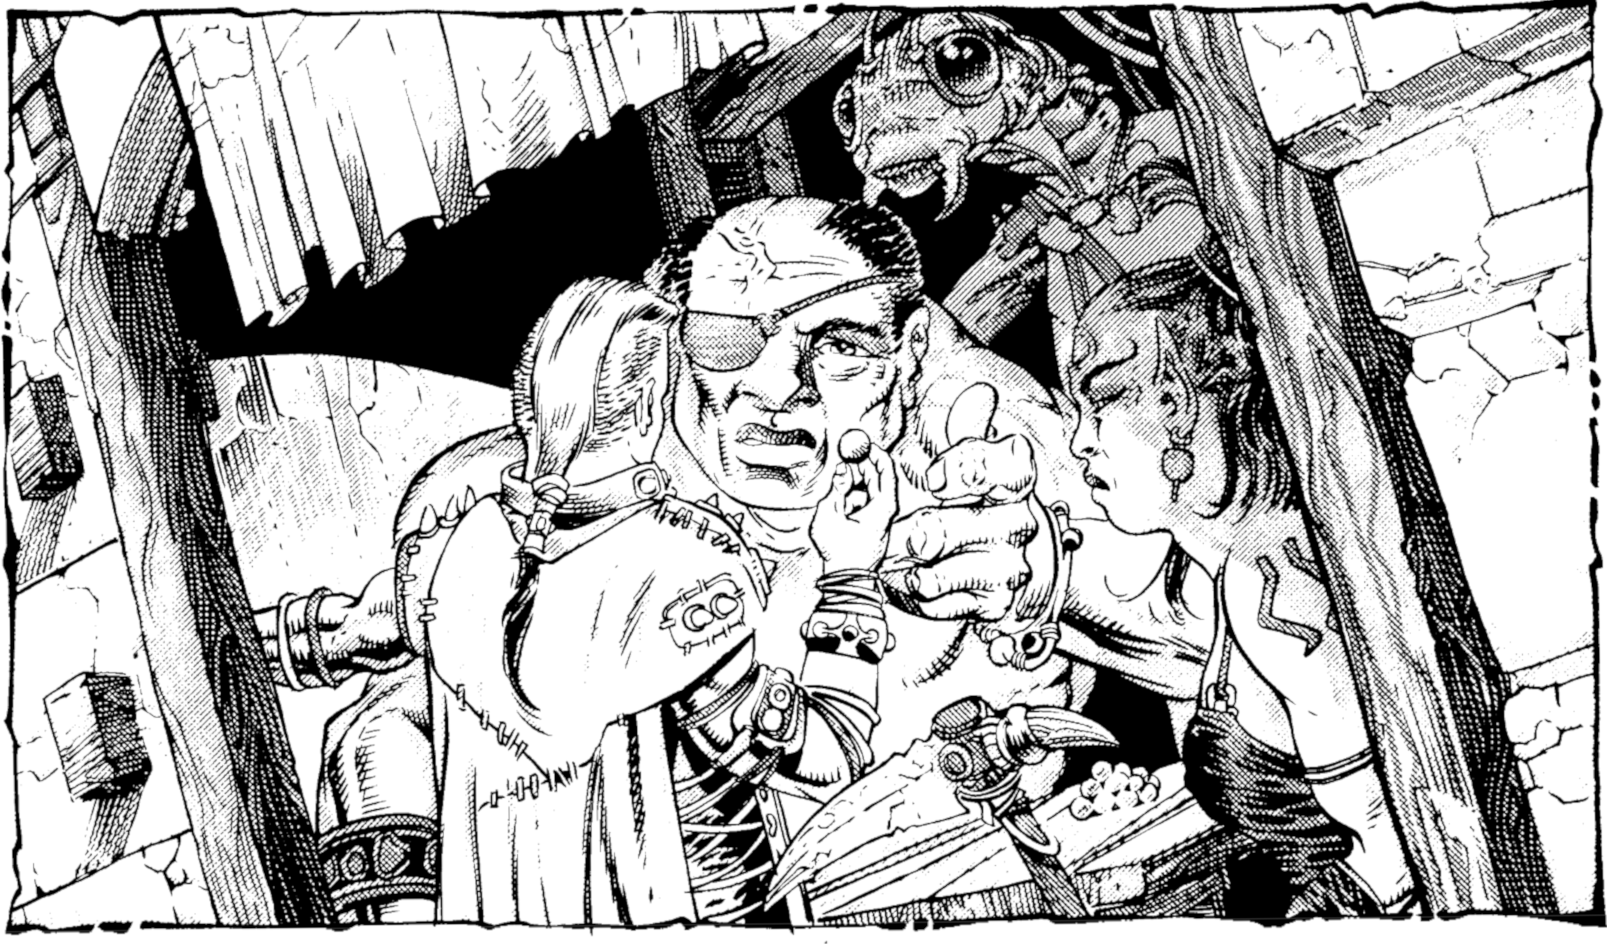
\includegraphics[width=\textwidth]{images/bribe-2.png}
\par\textit{\small\textcopyright Wizards of the Coast, 2020.}
\end{figure*}

\section{Wealth and Money}
\subsection{Coins}
All prices in {\tableheader Dark Sun} are given in terms of ceramic pieces, the most common coin. Ceramics are made from glazed clay and baked in batches once a year in a secure process supervised by the high templar that supervises the city's treasury. Bits are literally one-tenth parts of a ceramic piece---the ceramic pieces break easily into ten bits. Some cities' ceramic pieces have small holes that can be threaded onto a bracelet or necklace. The lowest unit of Athasian trade is the lead bead (bd).

Each of the city-states of the Tablelands produces its own currency. All cities use ceramic pieces as the most common coin, but also mint silver coins and, in some cases, rare and highly prized gold coins.

\Table{Currency Conversions}{l *4C}{
& \multicolumn{4}{c}{\tableheader Exchange Value}\\
\cmidrule[0.5pt]{2-5}
& \tableheader bd
& \tableheader bit
& \tableheader cp
& \tableheader sp\\
\textit{Lead bead (bd)}     & 1 & 1/10 & 1/100 & 1/1,000\\
\textit{Ceramic bit (bit)}  & 10 & 1 & 1/10 & 1/100\\
\textit{Ceramic piece (cp)} & 100 & 10 & 1 & 1/10\\
\textit{Silver piece (sp)}  & 1,000 & 100 & 10 & 1\\
\textit{Gold piece (gp)}    & 10,000 & 1000 & 100 & 10\\
}

\subsubsection{Moneychangers}
Adventurers that travel between cities will need to change their currency for local currency at each city they visit. With a couple of exceptions, the city-states have moneychangers available for incoming visitors. Located near the city gates and in large market places, moneychangers denote their business by hanging a large purple banner from their shop. The banners are always purple, but the moneychangers in each city-state display a different emblem on the banner, based on their city's standard.

Moneychangers charge each customer a fee to change coins. The fees differ by city and are summarized on \tabref{Moneychangers}.

\Table{Moneychangers}{C C}{
\tableheader City & \tableheader Exchange Rate\\
Balic   & 6\%\\
Draj    & 8\%\\
Gulg    & 10\%\\
Kurn    & 16\%\\
Nibenay & 14\%\\
Raam    & 12\%\\
Tyr     & 12\%\\
Urik    & 9\%\\
}

These fees are averages and may vary slightly. There are of course many unscrupulous money merchants who will charge as much as they can get away with. Moneychangers in Kurn are rare but a couple do exist. Since metal coins from any city-state are readily accepted by local merchants and no corresponding Kurnish coins exist there is little need to exchange such coins. There are, however, a few moneychangers willing to exchange ceramic pieces.

There are two cities that do not have moneychangers. Visitors to Celik have no need of a moneychangers, as merchants in that city take coins of all types. Nor are there any moneychangers in Eldaarich. Since Eldaarich has been shut off from the rest of the land for so long, visitors needing to exchange money have been nonexistent, so no moneychangers have set up business.

\subsection{Trade}
In general, the Athasian economy in the cities is relatively stable thanks to the Merchant Houses. Under normal conditions, supply is ample thanks to the caravans traveling back and forth between the cities. However, for smaller communities and trade outposts the price situation on certain goods can sway drastically. A raider attack or sandstorm can result in lack of necessities such as food and water, for which people will pay almost any amount of coin. Coins are not the only means of exchange. Barter and trade in commodities is widespread.

Dune traders commonly exchange trade goods without using currency, instead relying on a basic bartering system.


\Table{Trade Goods}{X r{1.3cm}}{
\tableheader Item & \tableheader Cost \\
One kilogram of salt & 4 bits \\
One kilogram of grain or faro & 6 bits \\
One kilogram of lead & 1 cp \\
One kilogram of nuts, or one kilogram of kank nectar & 2 cp \\
One square meter of cotton (cloth) & 4 cp \\
One kilogram of obsidian, or one square meter of silk, or one metric ton of water, or one erdlu & 10 cp \\
One herding kank, or one aprig & 50 cp \\
One kilogram of copper, or one male carru, or one inix & 100 cp \\
 One kilogram of iron, or one mekillot & 200 cp \\
One female carru & 300 cp \\
One kilogram of silver & 1,000 cp \\
One kilogram of gold & 10,000 cp \\
}

\subsection{Selling Loot}
In general, a character can sell something for half its listed price.

Trade goods are the exception to the half-price rule. A trade good, in this sense, is a valuable good that can be easily exchanged almost as if it were cash itself.

\section{Weapons}
Characters in a {\tableheader Dark Sun} game use a variety of weapons: some with direct counterparts in the real world, some without.

\subsection{Weapon Categories}
Weapons are grouped into several interlocking sets of categories.

These categories pertain to what training is needed to become proficient in a weapon's use (simple, martial, or exotic), the weapon's usefulness either in close combat (melee) or at a distance (ranged, which includes both thrown and projectile weapons), its relative encumbrance (light, one-handed, or two-handed), and its size (Small, Medium, or Large).

\textbf{Simple, Martial, and Exotic Weapons:} Anybody but a druid or wizard is proficient with all simple weapons. Barbarians, fighters, gladiators, and rangers are proficient with all simple and all martial weapons. Characters of other classes are proficient with an assortment of mainly simple weapons and possibly also some martial or even exotic weapons. A character who uses a weapon with which he or she is not proficient takes disadvantage on attack rolls.

\textbf{Melee and Ranged Weapons:} Melee weapons are used for making melee attacks, though some of them can be thrown as well. Ranged weapons are thrown weapons or projectile weapons that are not effective in melee.

\textit{Reach Weapons:} Glaives, guisarmes, lances, longspears, ranseurs, spiked chains, and whips are reach weapons. A reach weapon is a melee weapon that allows its wielder to strike at targets that aren't adjacent to him or her. Most reach weapons double the wielder's natural reach, meaning that a typical Small or Medium wielder of such a weapon can attack a creature 3 meters away, but not a creature in an adjacent square. A typical Large character wielding a reach weapon of the appropriate size can attack a creature 4.5 or 6 meters away, but not adjacent creatures or creatures up to 3 meters away.

Note: Small and Medium creatures wielding reach weapons threaten all squares 3 meters (2 squares) away, even diagonally. (This is an exception to the rule that 2 squares of diagonal distance is measured as 4.5 meters.)

\textit{Double Weapons:} Dire flails, dwarven urgroshes, gnome hooked hammers, orc double axes, quarterstaffs, and two-bladed swords are double weapons. A character can fight with both ends of a double weapon as if fighting with two weapons, but he or she incurs all the normal attack penalties associated with two-weapon combat, just as though the character were wielding a one-handed weapon and a light weapon.

The character can also choose to use a double weapon two handed, attacking with only one end of it. A creature wielding a double weapon in one hand can't use it as a double weapon---only one end of the weapon can be used in any given round.

\textit{Thrown Weapons:} Daggers, clubs, shortspears, spears, darts, javelins, throwing axes, light hammers, tridents, shuriken, and nets are thrown weapons. The wielder applies his or her Strength modifier to damage dealt by thrown weapons (except for splash weapons). It is possible to throw a weapon that isn't designed to be thrown (that is, a melee weapon that doesn't have a numeric entry in the Range Increment column on Table: Weapons), but a character who does so takes disadvantage on the attack roll. Throwing a light or one-handed weapon is a standard action, while throwing a two-handed weapon is a full-round action. Regardless of the type of weapon, such an attack scores a threat only on a natural roll of 20 and deals double damage on a critical hit. Such a weapon has a range increment of 3 meters.

\textit{Projectile Weapons:} Light crossbows, slings, heavy crossbows, shortbows, composite shortbows, longbows, composite longbows, hand crossbows, and repeating crossbows are projectile weapons. Most projectile weapons require two hands to use (see specific weapon descriptions). A character gets no Strength bonus on damage rolls with a projectile weapon unless it's a specially built composite shortbow, specially built composite longbow, or sling. If the character has a penalty for low Strength, apply it to damage rolls when he or she uses a bow or a sling.

\textit{Ammunition:} Projectile weapons use ammunition: arrows (for bows), bolts (for crossbows), or sling bullets (for slings). When using a bow, a character can draw ammunition as a free action; crossbows and slings require an action for reloading. Generally speaking, ammunition that hits its target is destroyed or rendered useless, while normal ammunition that misses has a 50\% chance of being destroyed or lost.

Although they are thrown weapons, shuriken are treated as ammunition for the purposes of drawing them, crafting masterwork or otherwise special versions of them (see Masterwork Weapons), and what happens to them after they are thrown.

\textbf{Light, One-Handed, and Two-Handed Melee Weapons:} This designation is a measure of how much effort it takes to wield a weapon in combat. It indicates whether a melee weapon, when wielded by a character of the weapon's size category, is considered a light weapon, a one-handed weapon, or a two-handed weapon.

\textit{Light:} A light weapon is easier to use in one's off hand than a one-handed weapon is, and it can be used while grappling. A light weapon is used in one hand. Add the wielder's Strength bonus (if any) to damage rolls for melee attacks with a light weapon if it's used in the primary hand, or one-half the wielder's Strength bonus if it's used in the off hand. Using two hands to wield a light weapon gives no advantage on damage; the Strength bonus applies as though the weapon were held in the wielder's primary hand only.

An unarmed strike is always considered a light weapon.

\textit{One-Handed:} A one-handed weapon can be used in either the primary hand or the off hand. Add the wielder's Strength bonus to damage rolls for melee attacks with a one-handed weapon if it's used in the primary hand, or \onehalf his or her Strength bonus if it's used in the off hand. If a one-handed weapon is wielded with two hands during melee combat, add 1\onehalf times the character's Strength bonus to damage rolls.

\textit{Two-Handed:} Two hands are required to use a two-handed melee weapon effectively. Apply 1\onehalf times the character's Strength bonus to damage rolls for melee attacks with such a weapon.

\textbf{Weapon Size:} Every weapon has a size category. This designation indicates the size of the creature for which the weapon was designed.

\Table{Larger and Smaller Weapon Damage}{l C C C C C}{
\tableheader Example Weapon & \tableheader Tiny & \tableheader Small & \tableheader Medium & \tableheader Large & \tableheader Huge \\
Shuriken & -- & 1 & 1d2 & 1d3 & 1d4\\
Gauntlet & 1 & 1d2 & 1d3 & 1d4 & 1d6\\
Dagger & 1d2 & 1d3 & 1d4 & 1d6 & 1d8\\
Shortspear & 1d3 & 1d4 & 1d6 & 1d8 & 2d6\\
Falchion & 1d4 & 1d6 & 2d4 & 2d6 & 3d6\\
Longsword & 1d4 & 1d6 & 1d8 & 2d6 & 3d6\\
Bastard Sword & 1d6 & 1d8 & 1d10 & 2d8 & 3d8\\
Greataxe & 1d8 & 1d10 & 1d12 & 3d6 & 4d6\\
Greatsword & 1d8 & 1d10 & 2d6 & 3d6 & 4d6\\
}

A weapon's size category isn't the same as its size as an object. Instead, a weapon's size category is keyed to the size of the intended wielder. In general, a light weapon is an object two size categories smaller than the wielder, a one-handed weapon is an object one size category smaller than the wielder, and a two-handed weapon is an object of the same size category as the wielder.

\textit{Inappropriately Sized Weapons:} A creature can't make optimum use of a weapon that isn't properly sized for it. A cumulative $-2$ penalty applies on attack rolls for each size category of difference between the size of its intended wielder and the size of its actual wielder. If the creature isn't proficient with the weapon disadvantage also applies.

The measure of how much effort it takes to use a weapon (whether the weapon is designated as a light, one-handed, or two-handed weapon for a particular wielder) is altered by one step for each size category of difference between the wielder's size and the size of the creature for which the weapon was designed. If a weapon's designation would be changed to something other than light, one-handed, or two-handed by this alteration, the creature can't wield the weapon at all.

\textbf{Improvised Weapons:} Sometimes objects not crafted to be weapons nonetheless see use in combat. Because such objects are not designed for this use, any creature that uses one in combat is considered to be nonproficient with it and takes disadvantage on attack rolls made with that object. To determine the size category and appropriate damage for an improvised weapon, compare its relative size and damage potential to the weapon list to find a reasonable match. An improvised weapon scores a threat on a natural roll of 20 and deals double damage on a critical hit. An improvised thrown weapon has a range increment of 3 meters.

\subsubsection{Metal Weapons}
Metal is rare on Athas, and many weapons ordinarily crafted using metal components are extremely expensive. Unworked iron is worth 100 cp per pound on average, but can cost much, much more in some places. Worked metal is even more expensive, as craftsmen who actually know how to craft metal items are rare at best. Most metal weapons are items dating back to the Green Age, or have been crafted from the meager resources of Tyr's iron mines.

Due to the rarity of metal, weapons and other items constructed primarily from metal are priced at in gp, e.g., a metal longsword costs 15 gp (or 1,500 cp). These weapons provide +1 bonus on damage rolls.

Due to the extremely high cost of metal weaponry, most weapons are constructed from inferior, but functional, materials instead on Athas. Most common are bone and stone such as flint or obsidian, but treated wood is sometimes used as well. Metal weapons constructed from inferior materials, such as bone longsword or an axe with a head made from stone, suffer a $-1$ penalty to attack and damage rolls. This penalty cannot reduce damage dealt below 1.

Furthermore, due to the rarity of metal, Athas has its share of unique weapons designed to be constructed from non-metal materials; as such, they do not suffer from the inferior materials penalties described above.

\NamedWeaponTable{Simple Weapons}{
\WeaponType{Unarmed Attacks}\\
Gauntlet
	& 2 cp & 4 cp & 1d2 & 1d3 & 1d4 & $\times2$ & & 0.25 kg& 0.5 kg& 1 kg & Bludgeoning\\
Unarmed strike
	& & & 1d2 & 1d3 & 1d4 & $\times2$ & & & & & Blud. non-lethal\\

\WeaponType{Light Melee Weapons}\\
Dagger
	& 2 cp & 4 cp & 1d3 & 1d4 & 1d6 & 19--20/$\times2$ & 3 m & 0.25 kg & 0.5 kg & 1 kg & Pierc. or slash.\\
Pushik
	& 4 cp & 8 cp & 1d3 & 1d4 & 1d6 & $\times3$ & & 0.25 kg & 0.5 kg & 1 kg & Piercing\\

\WeaponType{One-Handed Melee Weapons}\\
Club
	& & & 1d4 & 1d6 & 1d8 & $\times2$ & 3 m & 0.75 kg & 1.5 kg & 3 kg & Bludgeoning\\
Quabone
	& 3 cp & 6 cp & 1d4 & 1d6 & 1d8 & $\times2$ & & 1 kg & 2 kg & 4 kg & Bludgeoning\\
Shortspear
	& 1 cp & 2 cp & 1d4 & 1d6 & 1d8 & $\times2$ & 6 m & 0.75 kg & 1.5 kg & 3 kg & Piercing\\
Tonfa
	& 5 cp & 10 cp & 1d3 & 1d4 & 1d6 & $\times2$ & & 0.5 kg & 1 kg & 2 kg & Bludgeoning\\

\WeaponType{Two-Handed Melee Weapons}\\
Great tonfa
	& 10 cp & 20 cp & 1d4 & 1d6 & 1d8 & $\times2$ & & 1.25 kg & 2.5 kg & 5 kg & Bludgeoning\\
Longspear\footnotemark[1]
	& 5 cp & 10 cp & 1d6 & 1d8 & 2d6 & $\times3$ &  & 2.25 kg & 4.5 kg & 9 kg & Piercing\\
Quarterstaff\footnotemark[2]
	& & & 1d4 1d4 & 1d6 1d6 & 1d8 1d8 & $\times2$ & & 1 kg & 2 kg & 4 kg & Bludgeoning\\
Spear
	& 2 cp & 4 cp & 1d6 & 1d8 & 2d6 & $\times3$ & 6 m & 1.5 kg & 3 kg & 6 kg & Piercing\\

\WeaponType{Ranged Weapons}\\
Blowgun
	& 5 cp & 10 cp & 1 & 1d2 & 1d3 & $\times2$ & 3 m & 1 kg & 2 kg & 4 kg & Piercing\\
\Projectile{Needles, blowgun (20)}{1 cp}{2 cp}{}{}{}\\
Crossbow, heavy
	& 50 cp & 100 cp & 1d8 & 1d10 & 2d8 & 19--20/$\times2$ & 36 m & 2 kg & 4 kg & 8 kg & Piercing\\
\Projectile{Bolts, crossbow (10)}{1 cp}{2 cp}{0.25 kg}{0.5 kg}{1 kg}\\
Crossbow, light
	& 35 cp & 70 cp & 1d6 & 1d8 & 2d6 & 19--20/$\times2$ & 24 m & 1 kg & 2 kg & 4 kg & Piercing\\
\Projectile{Bolts, crossbow (10)}{1 cp}{2 cp}{0.25 kg}{0.5 kg}{1 kg}\\
Dart
	& 5 bits & 1 cp & 1d3 & 1d4 & 1d6 & $\times2$ & 6 m & 0.12 kg & 0.25 kg & 0.5 kg & Piercing\\
Javelin
	& 1 cp & 2 cp & 1d4 & 1d6 & 1d8 & $\times2$ & 9 m & 0.5 kg & 1 kg & 2 kg & Piercing\\
Pelota
	& 2 cp & 4 cp & 1d3 & 1d4 & 1d6 & $\times2$ & 3 m & 0.25 kg & 0.5 kg & 1 kg & Blud. and pierc.\\
Sling
	& & & 1d3 & 1d4 & 1d6 & $\times2$ & 15 m & & & & Bludgeoning\\
\Projectile{Bullets, sling (10)}{1 bit}{2 bits}{0.25 kg}{0.5 kg}{1 kg}\\

\BigTableNote{12}{1 Reach weapon}\\
\BigTableNote{12}{2 Double weapon}\\
}

\NamedWeaponTable{Martial Weapons}{
\WeaponType{Light Melee Weapons}\\
Forearm Axe
	& 30 cp & 60 cp & 1d3 & 1d4 & 1d6 & $\times3$ & & 1.5 kg & 3 kg & 6 kg & Slashing\\
Macahuitl, small
	& 20 cp & 40 cp & 1d4 & 1d6 & 1d8 & $\times2$ & & 0.5 kg & 1 kg & 2 kg & Slashing\\
Sap
	& 1 cp & 2 cp & 1d4 & 1d6 & 1d8 & $\times2$ & & 0.5 kg & 1 kg & 2 kg & Blud. non-lethal\\
Shield, light
	& $\star$ & $\star$ & 1d2 & 1d3 & 1d4 & $\times2$ & & $\star$ & $\star$ & $\star$ & Bludgeoning\\
Slodak
	& 18 cp & 36 cp & 1d4 & 1d6 & 1d8 & $\times2$ & & 1 kg & 2 kg & 4 kg & Slashing\\
Spiked armor
	& $\star$ & $\star$ & 1d4 & 1d6 & 1d8 & $\times2$ & & $\star$ & $\star$ & $\star$ & Piercing\\
Spiked shield, light
	& $\star$ & $\star$ & 1d3 & 1d4 & 1d6 & $\times2$ & & $\star$ & $\star$ & $\star$ & Piercing\\
Tortoise blade
	& 20 cp & 40 cp & 1d3 & 1d4 & 1d6 & 20/$\times2$ & & 0.5 kg & 1 kg & 2 kg & Piercing\\

\WeaponType{One-Handed Melee Weapons}\\
Alak
	& 7 cp & 14 cp & 1d4 & 1d6 & 1d8 & $\times3$ & & 1.5 kg & 3 kg & 6 kg & Piercing\\
Alhulak\footnotemark[1]
	& 40 cp & 80 cp & 1d4 & 1d6 & 1d8 & $\times3$ & & 2.25 kg & 4.5 kg & 9 kg & Piercing\\
Carrikal
	& 10 cp & 20 cp & 1d6 & 1d8 & 2d6 & $\times3$ & & 1.5 kg & 3 kg & 6 kg & Slashing\\
Impaler
	& 8 cp & 16 cp & 1d4 & 1d6 & 1d8 & $\times4$ & & 1.25 kg & 2.5 kg & 5 kg & Piercing\\
Macahuitl
	& 35 cp & 70 cp & 1d6 & 1d8 & 2d6 & $\times2$ & & 1.25 kg & 2.5 kg & 5 kg & Slashing\\
Shield, heavy
	& $\star$ & $\star$ & 1d3 & 1d4 & 1d6 & $\times2$ & & $\star$ & $\star$ & $\star$ & Bludgeoning\\
Spiked shield, heavy
	& $\star$ & $\star$ & 1d4 & 1d6 & 1d8 & $\times2$ & & $\star$ & $\star$ & $\star$ & Piercing\\

\WeaponType{Two-Handed Melee Weapons}\\
Club, datchi\footnotemark[1]
	& 5 cp & 10 cp & 1d6 & 1d8 & 2d6 & $\times3$ & & 2.5 kg & 5 kg & 10 kg & Bludgeoning\\
Crusher, Fixed\footnotemark[1]
	& 60 cp & 120 cp & 1d6 & 1d8 & 2d6 & $\times2$ & & 3 kg & 6 kg & 12 kg & Bludgeoning\\
Gouge
	& 20 cp & 40 cp & 1d8 & 1d10 & 2d8 & $\times3$ & & 3 kg & 6 kg & 12 kg & Piercing\\
Greatclub
	& 5 cp & 10 cp & 1d8 & 1d10 & 2d8 & $\times2$ & & 2 kg & 4 kg & 8 kg & Bludgeoning\\
Lance
	& 10 cp & 20 cp & 1d6 & 1d8 & 2d6 & $\times3$ & & 2.5 kg & 5 kg & 10 kg & Piercing\\
Macahuitl, Great
	& 50 cp & 100 cp & 1d10 & 2d6 & 3d6 & $\times2$ & & 3 kg & 6 kg & 12 kg & Slashing\\
Maul
	& 25 cp & 50 cp & 1d10 & 1d12 & 3d6 & $\times2$ & & 2.5 kg & 5 kg & 10 kg & Bludgeoning\\
Shield, long
	& $\star$ & $\star$ & 1d4 & 1d6 & 1d8 & $\times2$ & & $\star$ & $\star$ & $\star$ & Bludgeoning\\
Spiked shield, long
	& $\star$ & $\star$ & 1d6 & 1d8 & 2d6 & $\times2$ & & $\star$ & $\star$ & $\star$ & Piercing\\
Tkaesali\footnotemark[1]
	& 8 cp & 16 cp & 1d8 & 1d10 & 2d8 & $\times3$ & & 3.75 kg & 7.5 kg & 15 kg & Slashing\\
Trikal
	& 10 cp & 20 cp & 1d6 & 1d8 & 2d6 & $\times3$ & & 1.75 kg & 3.5 kg & 7 kg & Slashing\\

\WeaponType{Ranged Weapons}\\
Atlatl
	& 25 cp & 50 cp & 1d4 & 1d6 & 1d8 & $\times3$ & 12 m & 1.5 kg & 3 kg & 6 kg & Piercing\\
\Projectile{Javeli, atlatl}{2 cp}{4 cp}{0.5 kg}{1 kg}{2 kg}\\
Crossbow, fixed
	& 200 cp & 400 cp & 1d12 & 2d8 & 3d8 & 19--20/$\times2$ & 45 m & 25 kg & 50 kg & 100 kg & Piercing\\
\Projectile{Bolts (10)}{3 cp}{6 cp}{0.75 kg}{1.5 kg}{3 kg}\\
Longbow
	& 75 cp & 150 cp & 1d6 & 1d8 & 2d6 & $\times3$ & 30 m & 0.75 kg & 1.5 kg & 3 kg & Piercing\\
\Projectile{Arrows (10)}{1 cp}{2 cp}{0.75 kg}{1.5 kg}{3 kg}\\
Longbow, composite
	& 100 cp & 200 cp & 1d6 & 1d8 & 2d6 & $\times3$ & 33 m & 0.75 kg & 1.5 kg & 3 kg & Piercing\\
\Projectile{Arrows (10)}{1 cp}{2 cp}{0.75 kg}{1.5 kg}{3 kg}\\
Shortbow
	& 30 cp & 60 cp & 1d4 & 1d6 & 1d8 & $\times3$ & 18 m & 0.5 kg & 1 kg & 2 kg & Piercing\\
\Projectile{Arrows (10)}{1 cp}{2 cp}{0.75 kg}{1.5 kg}{3 kg}\\
Shortbow, composite
	& 75 cp & 150 cp & 1d4 & 1d6 & 1d8 & $\times3$ & 21 m & 0.5 kg & 1 kg & 2 kg & Piercing\\
\Projectile{Arrows (10)}{1 cp}{2 cp}{0.75 kg}{1.5 kg}{3 kg}\\

\BigTableNote{12}{1 Reach weapon}\\
\BigTableNote{12}{$\star$ Inherent properties of the armor or shield. See Armor for details.}\\
}

\NamedWeaponTable{Exotic Weapons}{
\WeaponType{Light Melee Weapons}\\
Bard's Friend
	& 20 cp & 40 cp & 1d3 & 1d4 & 1d6 & 18--20/$\times2$ & & 0.25 kg & 0.5 kg & 1 kg & Piercing\\
Bard's Garrote
	& 200 cp & 400 cp & 1d6 & 2d4 & 2d6 & $\times2$ & & 0.25 kg & 0.5 kg & 1 kg & Blud. non-lethal\\
Ko
	& 1 cp & 2 cp & 1d3 & 1d4 & 1d6 & $\times4$ & & 0.75 kg & 1.5 kg & 3 kg & Piercing\\
Handfork
	& 20 cp & 40 cp & 1d3 & 1d4 & 1d6 & $\times2$ & & 0.5 kg & 1 kg & 2 kg & Slashing\\
Lajav
	& 8 cp & 16 cp & 1d3 & 1d4 & 1d6 & $\times4$ & & 2 kg & 4 kg & 8 kg & Bludgeoning\\
Nunchaku
	& 2 cp & 4 cp & 1d4 & 1d6 & 1d8 & $\times2$ & & 0.5 kg & 1 kg & 2 kg & Bludgeoning\\
Sai
	& 1 cp & 2 cp & 1d3 & 1d4 & 1d6 & $\times2$ & 3 m & 0.25 kg & 0.5 kg & 1 kg & Bludgeoning\\
Singing Sticks
	& 10 cp & 20 cp & 1d4 & 1d6 & 1d8 & $\times2$ & & 0.25 kg & 0.5 kg & 1 kg & Bludgeoning\\
Talid
	& 40 cp & 80 cp & 1d4 & 1d6 & 1d8 & 19--20/$\times2$ & & 1 kg & 2 kg & 4 kg & Piercing\\
Widow's Knife
	& 50 cp & 100 cp & 1d3 & 1d4 & 1d6 & $\times3$ & & 0.5 kg & 1 kg & 2 kg & Piercing\\
Wrist Razor
	& 15 cp & 30 cp & 1d4 & 1d6 & 1d8 & 18--20/$\times2$ & & 0.5 kg & 1 kg & 2 kg & Slashing\\

\WeaponType{One-Handed Melee Weapons}\\
Heartpick
	& 9 cp & 18 cp & 1d6 & 1d8 & 2d6 & $\times4$ & & 0.5 kg & 1 kg & 2 kg & Piercing\\
Master's Whip\footnotemark[1]
	& 25 cp & 50 cp & 1d2 & 1d3 & 1d4 & $\times2$ & & 1.25 kg & 2.5 kg & 5 kg & Slashing\\
Whip\footnotemark[1]
	& 1 cp & 2 cp & 1d2 & 1d3 & 1d4 & $\times2$ & & 0.5 kg & 1 kg & 2 kg & Slash. non-lethal\\

\WeaponType{Two-Handed Melee Weapons}\\
Cahulak\footnotemark[2]
	& 120 cp & 240 cp & 1d4 1d4 & 1d6 1d6 & 1d8 1d8 & $\times3$ & & 3 kg & 6 kg & 12 kg & Piercing\\
Crusher, free\footnotemark[1]
	& 18 cp & 36 cp & 1d8 & 1d10 & 2d8 & $\times2$ & & 3 kg & 6 kg & 12 kg & Bludgeoning\\
Dragon's paw\footnotemark[2]
	& 80 cp & 160 cp & 1d4 1d4 & 1d6 1d6 & 1d8 1d8 & 19--20/$\times2$ & & 2.25 kg & 4.5 kg & 9 kg & Piercing\\
Gythka\footnotemark[2]
	& 60 cp & 120 cp & 1d6 1d6 & 1d8 1d8 & 2d6 2d6 & $\times2$ & & 6.25 kg & 12.5 kg & 25 kg & Slashing\\
Lotulis\footnotemark[2]
	& 115 cp & 230 cp & 1d6 1d6 & 1d8 1d8 & 2d6 2d6 & 19--20/$\times2$ & & 2.25 kg & 4.5 kg & 9 kg & Slashing\\
Pike, weighted\footnotemark[2]
	& 75 cp & 150 cp & 1d6 1d4 & 1d8 1d6 & 2d6 1d8 & 19--20/$\times2$ & & 3.75 kg & 7.5 kg & 15 kg & Bludgeoning Piercing\\
Spear, double-tipped\footnotemark[2]
	& 20 cp & 40 cp & 1d6 1d6 & 1d8 1d8 & 2d6 2d6 & $\times3$ & 6 m & 1.5 kg & 3 kg & 6 kg & Piercing\\
Thanak
	& 20 cp & 40 cp & 1d10 & 2d6 & 3d6 & $\times3$ & & 2.5 kg & 5 kg & 10 kg & Slashing\\
Swatter
	& 100 cp & 200 cp & 1d12 & 2d8 & 3d8 & $\times4$ & & 8.75 kg & 17.5 kg & 35 kg & Bludgeoning\\
Mekillot sap\footnotemark[1]
	& 25 cp & 50 cp & 1d12 & 2d8 & 3d8 & $\times2$ & 3 m & 7.5 kg & 15 kg & 30 kg & Blud. non-lethal\\

\WeaponType{Ranged Weapons}\\
Blowgun, greater
	& 10 cp & 20 cp & 1d3 & 1d4 & 1d6 & $\times2$ & 3 m & 1 kg & 2 kg & 4 kg & Piercing\\
\Projectile{Darts, blowgun (10)}{1 cp}{2 cp}{0.25 kg}{0.5 kg}{1 kg}\\
Bolas
	& 5 cp & 10 cp & 1d3 & 1d4 & 1d6 & $\times2$ & 3 m & 0.5 kg & 1 kg & 2 kg & Blud. non-lethal\\
Chatkcha
	& 20 cp & 40 cp & 1d4 & 1d6 & 1d8 & $\times2$ & 6 m & 0.75 kg & 1.5 kg & 3 kg & Piercing\\
Crossbow, hand
	& 100 cp & 200 cp & 1d3 & 1d4 & 1d6 & 19--20/$\times2$ & 9 m & 0.5 kg & 1 kg & 2 kg & Piercing\\
\Projectile{Bolts (10)}{1 cp}{2 cp}{0.25 kg}{0.5 kg}{1 kg}\\
Crossbow, repeat. heavy
	& 400 cp & 800 cp & 1d8 & 1d10 & 2d8 & 19--20/$\times2$ & 36 m & 3 kg & 6 kg & 12 kg & Piercing\\
\Projectile{Bolts (5)}{1 cp}{2 cp}{0.25 kg}{0.5 kg}{1 kg}\\
Crossbow, repeating light
	& 250 cp & 500 cp & 1d6 & 1d8 & 2d6 & 19--20/$\times2$ & 24 m & 1.5 kg & 3 kg & 6 kg & Piercing\\
\Projectile{Bolts (5)}{1 cp}{2 cp}{0.25 kg}{0.5 kg}{1 kg}\\
Dejada
	& 20 cp & 40 cp & 1d4 & 1d6 & 1d8 & $\times2$ & 9 m & 0.5 kg & 1 kg & 2 kg & Piercing\\
\Projectile{Pelota, dejada}{2 cp}{4 cp}{0.25 kg}{0.5 kg}{1 kg}\\
Lasso
	& 2 cp & 4 cp & & & & $\times2$ & 3 m & 0.5 kg & 1 kg & 2 kg & Bludgeoning\\
Net
	& 20 cp & 40 cp & & & & & 3 m & 1.5 kg & 3 kg & 6 kg & \\
Skyhammer
	& 50 cp & 100 cp & 1d8 & 1d10 & 2d8 & $\times2$ & 4.5 m & 1.5 kg & 3 kg & 6 kg & Bludgeoning\\
Splashbow
	& 300 cp & 600 cp & 1d3 & 1d4 & 1d6 & $\times2$ & 18 m & 15 kg & 30 kg & 60 kg & Bludgeoning\\
~ Pelota, hinged
	& 5 cp & 10 cp & & & & $\times2$ & 4.5 m & 0.5 kg & 1 kg & 2 kg & Bludgeoning\\
Zerka
	& 30 cp & 60 cp & 1d6 & 1d8 & 2d6 & 18--20/$\times2$ & 9 m & 2.25 kg & 4.5 kg & 9 kg & Piercing\\

\BigTableNote{12}{1 Reach weapon}\\
\BigTableNote{12}{2 Double weapon}\\
}

\NamedWeaponTable{Metal Simple Weapons}{
\WeaponType{Light Melee Weapons}\\
Dagger, punching
	& 2 gp & 4 gp & 1d3 & 1d4 & 1d6 & $\times3$ & & 0.25 kg & 0.5 kg & 1 kg & Piercing\\
\InferiorWeapon{(bone or wood)}{1 cp}{2 cp}{0.12 kg}{0.25 kg}{0.5 kg}\\
\InferiorWeapon{(stone)}{1 cp}{2 cp}{0.5 kg}{1 kg}{2 kg}\\
Gauntlet, spiked
	& 25 sp & 5 gp & 1d3 & 1d4 & 1d6 & $\times2$ & & 0.25 kg & 0.5 kg & 1 kg & Piercing\\
\InferiorWeapon{(bone or wood)}{25 bits}{5 cp}{0.12 kg}{0.25 kg}{0.5 kg}\\
\InferiorWeapon{(stone)}{25 bits}{5 cp}{0.5 kg}{1 kg}{2 kg}\\
Mace, light
	& 5 gp & 10 gp & 1d4 & 1d6 & 1d8 & $\times2$ & & 1 kg & 2 kg & 4 kg & Bludgeoning\\
\InferiorWeapon{(bone or wood)}{25 bits}{5 cp}{0.5 kg}{1 kg}{2 kg}\\
\InferiorWeapon{(stone)}{25 bits}{5 cp}{2 kg}{4 kg}{8 kg}\\
Sickle
	& 6 gp & 12 gp & 1d4 & 1d6 & 1d8 & $\times2$ & & 0.5 kg & 1 kg & 2 kg & Slashing\\
\InferiorWeapon{(bone or wood)}{1 cp}{2 cp}{0.25 kg}{0.5 kg}{1 kg}\\
\InferiorWeapon{(stone)}{1 cp}{2 cp}{1 kg}{2 kg}{4 kg}\\

\WeaponType{One-Handed Melee Weapons}\\
Mace, heavy
	& 12 gp & 24 cp & 1d6 & 1d8 & 2d6 & $\times2$ & & 2 kg & 4 kg & 8 kg & Bludgeoning\\
\InferiorWeapon{(bone or wood)}{6 cp}{12 cp}{1 kg}{2 kg}{4 kg}\\
\InferiorWeapon{(stone)}{6 cp}{12 cp}{4 kg}{8 kg}{16 kg}\\
Morningstar
	& 8 gp & 16 gp & 1d6 & 1d8 & 2d6 & $\times2$ & & 1.5 kg & 3 kg & 6 kg & Blud. and pierc.\\
\InferiorWeapon{(bone or wood)}{4 cp}{8 cp}{0.75 kg}{1.5 kg}{3 kg}\\
\InferiorWeapon{(stone)}{4 cp}{8 cp}{3 kg}{6 kg}{12 kg}\\

\BigTableNote{12}{$\diamond$ Inferior material weapons suffer $-1$ penalty to attack and damage rolls.}\\
% \rowcolor{white}\\
\rowcolor{white}\\
}

\NamedWeaponTable{Metal Martial Weapons 1}{
\WeaponType{Light Melee Weapons}\\
Axe, throwing
	& 8 gp & 16 gp & 1d4 & 1d6 & 1d6 & $\times2$ & 3 m & 0.5 kg & 1 kg & 2 kg & Slashing\\
\InferiorWeapon{(bone or wood)}{4 cp}{8 cp}{0.25 kg}{0.5 kg}{1 kg}\\
\InferiorWeapon{(stone)}{4 cp}{8 cp}{1 kg}{2 kg}{4 kg}\\
Hammer, light
	& 1 gp & 2 gp & 1d3 & 1d4 & 1d4 & $\times2$ & 6 m & 0.5 kg & 1 kg & 2 kg & Bludgeoning\\
\InferiorWeapon{(bone or wood)}{5 bits}{1 cp}{0.25 kg}{0.5 kg}{1 kg}\\
\InferiorWeapon{(stone)}{5 bits}{1 cp}{1 kg}{2 kg}{4 kg}\\
Handaxe
	& 6 gp & 12 gp & 1d4 & 1d6 & 1d6 & $\times3$ & & 0.75 kg & 1.5 kg & 3 kg & Slashing\\
\InferiorWeapon{(bone or wood)}{3 cp}{6 cp}{0.37 kg}{0.75 kg}{1.5 kg}\\
\InferiorWeapon{(stone)}{3 cp}{6 cp}{1.5 kg}{3 kg}{6 kg}\\
Kukri
	& 8 gp & 16 gp & 1d3 & 1d4 & 1d6 & 18--20/$\times2$ & & 0.5 kg & 1 kg & 2 kg & Slashing\\
\InferiorWeapon{(bone or wood)}{4 cp}{8 cp}{0.25 kg}{0.5 kg}{1 kg}\\
\InferiorWeapon{(stone)}{4 cp}{8 cp}{1 kg}{2 kg}{4 kg}\\
Pick, light
	& 4 gp & 8 gp & 1d3 & 1d4 & 1d6 & $\times4$ & & 0.75 kg & 1.5 kg & 3 kg & Piercing\\
\InferiorWeapon{(bone or wood)}{2 cp}{4 cp}{0.37 kg}{0.75 kg}{1.5 kg}\\
\InferiorWeapon{(stone)}{2 cp}{4 cp}{1.5 kg}{3 kg}{6 kg}\\
Sword, short
	& 10 gp & 20 gp & 1d4 & 1d6 & 1d8 & 19--20/$\times2$ & & 0.5 kg & 1 kg & 2 kg & Piercing\\
\InferiorWeapon{(bone or wood)}{5 cp}{10 cp}{0.25 kg}{0.5 kg}{1 kg}\\
\InferiorWeapon{(stone)}{5 cp}{10 cp}{1 kg}{2 kg}{4 kg}\\

\WeaponType{One-Handed Melee Weapons}\\
Battleaxe
	& 10 gp & 20 gp & 1d6 & 1d8 & 2d6 & $\times3$ & & 1.5 kg & 3 kg & 6 kg & Slashing\\
\InferiorWeapon{(bone or wood)}{5 cp}{10 cp}{0.75 kg}{1.5 kg}{3 kg}\\
\InferiorWeapon{(stone)}{5 cp}{10 cp}{3 kg}{6 kg}{12 kg}\\
Flail
	& 8 gp & 16 gp & 1d6 & 1d8 & 2d6 & $\times2$ & & 1.25 kg & 2.5 kg & 5 kg & Bludgeoning\\
\InferiorWeapon{(bone or wood)}{4 cp}{8 cp}{0.62 kg}{1.25 kg}{2.5 kg}\\
\InferiorWeapon{(stone)}{4 cp}{8 cp}{2.5 kg}{5 kg}{10 kg}\\
Longsword
	& 15 gp & 30 gp & 1d6 & 1d8 & 2d6 & 19--20/$\times2$ & & 1 kg & 2 kg & 4 kg & Slashing\\
\InferiorWeapon{(bone or wood)}{75 bits}{15 cp}{0.5 kg}{1 kg}{2 kg}\\
\InferiorWeapon{(stone)}{75 bits}{15 cp}{2 kg}{4 kg}{8 kg}\\
Pick, heavy
	& 8 gp & 16 gp & 1d4 & 1d6 & 1d8 & $\times4$ & & 1.5 kg & 3 kg & 6 kg & Piercing\\
\InferiorWeapon{(bone or wood)}{4 cp}{8 cp}{0.75 kg}{1.5 kg}{3 kg}\\
\InferiorWeapon{(stone)}{4 cp}{8 cp}{3 kg}{6 kg}{12 kg}\\
Rapier
	& 20 gp & 40 gp & 1d4 & 1d6 & 1d8 & 18--20/$\times2$ & & 0.5 kg & 1 kg & 2 kg & Piercing\\
\InferiorWeapon{(bone or wood)}{10 cp}{20 cp}{0.25 kg}{0.5 kg}{1 kg}\\
\InferiorWeapon{(stone)}{10 cp}{20 cp}{1 kg}{2 kg}{4 kg}\\
Scimitar
	& 15 gp & 30 gp & 1d4 & 1d6 & 1d8 & 18--20/$\times2$ & & 1 kg & 2 kg & 4 kg & Slashing\\
\InferiorWeapon{(bone or wood)}{75 bits}{15 cp}{0.5 kg}{1 kg}{2 kg}\\
\InferiorWeapon{(stone)}{75 bits}{15 cp}{2 kg}{4 kg}{8 kg}\\
Trident
	& 15 gp & 30 gp & 1d6 & 1d8 & 2d6 & $\times2$ & 3 m & 1 kg & 2 kg & 4 kg & Piercing\\
\InferiorWeapon{(bone or wood)}{75 bits}{15 cp}{0.5 kg}{1 kg}{2 kg}\\
\InferiorWeapon{(stone)}{75 bits}{15 cp}{2 kg}{4 kg}{8 kg}\\
Warhammer
	& 12 gp & 24 gp & 1d6 & 1d8 & 2d6 & $\times3$ & & 1.25 kg & 2.5 kg & 5 kg & Bludgeoning\\
\InferiorWeapon{(bone or wood)}{6 cp}{12 cp}{0.62 kg}{1.25 kg}{2.5 kg}\\
\InferiorWeapon{(stone)}{6 cp}{12 cp}{2.5 kg}{5 kg}{10 kg}\\

\BigTableNote{12}{$\diamond$ Inferior material weapons suffer $-1$ penalty to attack and damage rolls.}\\
\rowcolor{white}\\
\rowcolor{white}\\
}

\NamedWeaponTable{Metal Martial Weapons 2}{
\WeaponType{Two-Handed Melee Weapons}\\
Falchion
	& 75 gp & 150 gp & 1d6 & 2d4 & 2d6 & 18--20/$\times2$ & & 2 kg & 4 kg & 8 kg & Slashing\\
\InferiorWeapon{(bone or wood)}{32.5 cp}{75 cp}{1 kg}{2 kg}{4 kg}\\
\InferiorWeapon{(stone)}{32.5 cp}{75 cp}{4 kg}{8 kg}{16 kg}\\
Glaive\footnotemark[1]
	& 8 gp & 16 gp & 1d8 & 1d10 & 2d8 & $\times3$ & & 2.5 kg & 5 kg & 10 kg & Slashing\\
\InferiorWeapon{(bone or wood)}{4 cp}{8 cp}{1.25 kg}{2.5 kg}{5 kg}\\
\InferiorWeapon{(stone)}{4 cp}{8 cp}{5 kg}{10 kg}{20 kg}\\
Greataxe
	& 20 gp & 40 gp & 1d10 & 1d12 & 3d6 & $\times3$ & & 3 kg & 6 kg & 12 kg & Slashing\\
\InferiorWeapon{(bone or wood)}{10 cp}{20 cp}{1.5 kg}{3 kg}{6 kg}\\
\InferiorWeapon{(stone)}{10 cp}{20 cp}{6 kg}{12 kg}{24 kg}\\
Flail, heavy
	& 15 gp & 30 gp & 1d8 & 1d10 & 2d8 & 19--20/$\times2$ & & 2.5 kg & 5 kg & 10 kg & Bludgeoning\\
\InferiorWeapon{(bone or wood)}{75 bits}{15 cp}{1.25 kg}{2.5 kg}{5 kg}\\
\InferiorWeapon{(stone)}{75 bits}{15 cp}{5 kg}{10 kg}{20 kg}\\
Greatsword
	& 50 gp & 100 gp & 1d10 & 2d6 & 3d6 & 19--20/$\times2$ & & 2 kg & 4 kg & 8 kg & Slashing\\
\InferiorWeapon{(bone or wood)}{25 cp}{50 cp}{1 kg}{2 kg}{4 kg}\\
\InferiorWeapon{(stone)}{25 cp}{50 cp}{4 kg}{8 kg}{16 kg}\\
Guisarme\footnotemark[1]
	& 45 sp & 9 gp & 1d6 & 2d4 & 2d6 & $\times3$ & & 3 kg & 6 kg & 12 kg & Slashing\\
\InferiorWeapon{(bone or wood)}{25 bits}{45 bits}{0.25 kg}{0.5 kg}{1 kg}\\
\InferiorWeapon{(stone)}{25 bits}{45 bits}{1 kg}{2 kg}{4 kg}\\
Halberd
	& 10 gp & 20 gp & 1d8 & 1d10 & 2d8 & $\times3$ & & 3 kg & 6 kg & 12 kg & Pierc. or slash.\\
\InferiorWeapon{(bone or wood)}{5 cp}{10 cp}{1.5 kg}{3 kg}{6 kg}\\
\InferiorWeapon{(stone)}{5 cp}{10 cp}{6 kg}{12 kg}{24 kg}\\
Ranseur\footnotemark[1]
	& 10 gp & 20 gp & 1d6 & 2d4 & 2d6 & $\times3$ & & 3 kg & 6 kg & 12 kg & Piercing\\
\InferiorWeapon{(bone or wood)}{5 cp}{10 cp}{1.5 kg}{3 kg}{6 kg}\\
\InferiorWeapon{(stone)}{5 cp}{10 cp}{6 kg}{12 kg}{24 kg}\\
Scythe
	& 18 gp & 36 gp & 1d6 & 2d4 & 2d6 & $\times4$ & & 2.5 kg & 5 kg & 10 kg & Pierc. or slash.\\
\InferiorWeapon{(bone or wood)}{9 cp}{18 cp}{1.25 kg}{2.5 kg}{5 kg}\\
\InferiorWeapon{(stone)}{9 cp}{18 cp}{5 kg}{10 kg}{20 kg}\\

\WeaponType{Ranged Weapons}\\
\Projectile{Arrows, metal (20)}{1 gp}{2 gp}{0.75 kg}{1.5 kg}{3 kg}\\


\BigTableNote{12}{1 Reach weapon}\\
\BigTableNote{12}{$\diamond$ Inferior material weapons suffer $-1$ penalty to attack and damage rolls.}\\
}

\NamedWeaponTable{Metal Exotic Weapons}{
\WeaponType{Light Melee Weapons}\\
Kama
	& 2 gp & 4 gp & 1d4 & 1d6 & 1d8 & $\times2$ & & 0.5 kg & 1 kg & 2 kg & Slashing\\
\InferiorWeapon{(bone or wood)}{1 cp}{2 cp}{0.25 kg}{0.5 kg}{1 kg}\\
\InferiorWeapon{(stone)}{1 cp}{2 cp}{1 kg}{2 kg}{4 kg}\\
\WeaponType{One-Handed Melee Weapons}\\
Longblade, elven
	& 15 gp & 30 gp & 1d6 & 1d8 & 2d6 & 18--20/$\times2$ & & 0.75 kg & 1.5 kg & 3 kg & Slashing\\
\InferiorWeapon{(bone or wood)}{8 cp}{15 cp}{0.37 kg}{0.75 kg}{1.5 kg}\\
\InferiorWeapon{(stone)}{8 cp}{15 cp}{1.5 kg}{3 kg}{6 kg}\\
Sword, bastard
	& 35 gp & 70 gp & 1d8 & 1d10 & 2d8 & 19--20/$\times2$ & & 1.5 kg & 3 kg & 6 kg & Slashing\\
\InferiorWeapon{(bone or wood)}{18 cp}{35 cp}{0.75 kg}{1.5 kg}{3 kg}\\
\InferiorWeapon{(stone)}{18 cp}{35 cp}{3 kg}{6 kg}{12 kg}\\
Waraxe, dwarven
	& 30 gp & 60 gp & 1d8 & 1d10 & 2d8 & $\times3$ & & 2 kg & 4 kg & 8 kg & Slashing\\
\InferiorWeapon{(bone or wood)}{15 cp}{30 cp}{1 kg}{2 kg}{4 kg}\\
\InferiorWeapon{(stone)}{15 cp}{30 cp}{4 kg}{8 kg}{16 kg}\\

\WeaponType{Two-Handed Melee Weapons}\\
Chain, spiked\footnotemark[1]
	& 25 gp & 50 gp & 1d6 & 2d4 & 2d6 & $\times2$ & & 2.5 kg & 5 kg & 10 kg & Piercing\\
\InferiorWeapon{(bone or wood)}{13 cp}{25 cp}{1.25 kg}{2.5 kg}{5 kg}\\
\InferiorWeapon{(stone)}{13 cp}{25 cp}{5 kg}{10 kg}{20 kg}\\
Flail, dire
	& 90 gp & 180 gp & 1d6 1d6 & 1d8 1d8 & 2d6 2d6 & $\times2$ & & 2.5 kg & 5 kg & 10 kg & Bludgeoning\\
\InferiorWeapon{(bone or wood)}{45 cp}{90 cp}{1.25 kg}{2.5 kg}{5 kg}\\
\InferiorWeapon{(stone)}{45 cp}{90 cp}{5 kg}{10 kg}{20 kg}\\
Sword, two-bladed\footnotemark[2]
	& 100 gp & 200 gp & 1d6 1d6 & 1d8 1d8 & 2d6 2d6 & 19--20/$\times2$ & & 2.5 kg & 5 kg & 10 kg & Slashing\\
\InferiorWeapon{(bone or wood)}{45 cp}{90 cp}{1.25 kg}{2.5 kg}{5 kg}\\
\InferiorWeapon{(stone)}{45 cp}{90 cp}{5 kg}{10 kg}{20 kg}\\
Urgrosh, dwarven\footnotemark[2]
	& 50 gp & 100 gp & 1d6 1d4 & 1d8 1d6 & 2d6 1d8 & $\times3$ & & 3 kg & 6 kg & 12 kg & Slashing Piercing\\
\InferiorWeapon{(bone or wood)}{25 cp}{50 cp}{1.5 kg}{3 kg}{6 kg}\\
\InferiorWeapon{(stone)}{25 cp}{50 cp}{6 kg}{12 kg}{24 kg}\\

\WeaponType{Ranged Weapons}\\
Shuriken (5)
	& 1 gp & 2 gp & 1 & 1d2 & 1d3 & $\times2$ & 3 m & 0.25 kg & 0.5 kg & 1 kg & Piercing\\
\InferiorWeapon{(bone or wood)}{5 bits}{1 cp}{0.12 kg}{0.25 kg}{0.5 kg}\\
\InferiorWeapon{(stone)}{5 bits}{1 cp}{0.5 kg}{1 kg}{2 kg}\\

\BigTableNote{12}{1 Reach weapon}\\
\BigTableNote{12}{2 Double weapon}\\
\BigTableNote{12}{$\diamond$ Inferior material weapons suffer $-1$ penalty to attack and damage rolls.}\\
}



\subsection{Weapon Qualities}
Here is the format for weapon entries (given as column headings on each weapon table).

\textbf{Cost:} This value is the weapon's cost in gold pieces (gp), silver pieces (sp), ceramic pieces (cp) or ceramic bits (bits). The cost includes miscellaneous gear that goes with the weapon.

This cost is the same for a Small or Medium version of the weapon. A Large version costs twice the listed price.

\textbf{Damage:} The Damage columns give the damage dealt by the weapon on a successful hit. There are three columns for different weapon sizes: ``S'' for Small weapons, ``M'' for Medium weapons, and ``L'' for Large weapons. If two damage ranges are given then the weapon is a double weapon. Use the second damage figure given for the double weapon's extra attack. \tabref{Larger and Smaller Weapon Damage} gives weapon damage values for weapons of various sizes.

\textbf{Critical:} The entry in this column notes how the weapon is used with the rules for critical hits. When your character scores a critical hit, roll the damage two, three, or four times, as indicated by its critical multiplier (using all applicable modifiers on each roll), and add all the results together.

\textit{Exception:} Extra damage over and above a weapon's normal damage is not multiplied when you score a critical hit.

\textit{\multiplied2:} The weapon deals double damage on a critical hit.

\textit{\multiplied3:} The weapon deals triple damage on a critical hit.

\textit{\multiplied4:} The weapon deals quadruple damage on a critical hit.

\textit{19--20/\multiplied2:} The weapon scores a threat on a natural roll of 19 or 20 (instead of just 20) and deals double damage on a critical hit. (The weapon has a threat range of 19--20.)

\textit{18--20/\multiplied2:} The weapon scores a threat on a natural roll of 18, 19, or 20 (instead of just 20) and deals double damage on a critical hit. (The weapon has a threat range of 18--20.)

\textbf{Range Increment:} Any attack at less than this distance is not penalized for range. However, each full range increment imposes a cumulative $-2$ penalty on the attack roll. A thrown weapon has a maximum range of five range increments. A projectile weapon can shoot out to ten range increments.

\textbf{Weight:} There are three columns for the weight of a weapon: ``S'' for Small weapons, ``M'' for Medium weapons, and ``L'' for Large weapons.

\textbf{Type:} Weapons are classified according to the type of damage they deal: bludgeoning, piercing, or slashing. Some monsters may be resistant or immune to attacks from certain types of weapons.

Some weapons deal damage of multiple types. If a weapon is of two types, the damage it deals is not half one type and half another; all of it is both types. Therefore, a creature would have to be immune to both types of damage to ignore any of the damage from such a weapon.

In other cases, a weapon can deal either of two types of damage. In a situation when the damage type is significant, the wielder can choose which type of damage to deal with such a weapon.

\textbf{Special:} Some weapons have special features. See the weapon descriptions for details.

\subsection{Weapon Descriptions}
Weapons found on \tabref{Weapons} that have special options for the wielder (``you'') are described below. Splash weapons are described under Special Substances and Items.

\textbf{Alak:} An alak consists of a 60 centemeters long shaft of bone or wood, with four serrated bones tied to the sharp end, like the four prongs of a grappling hook.

When using an alak, you get a +2 bonus on the opposed attack roll when attempting to disarm an opponent (including the roll to avoid being disarmed if you fail to disarm your opponent). 

\textbf{Alhulak:} The alhulak consists of an alak tied to a 1.5 meter long leather cord, which wraps around your wrist at the other end. An alhulak has reach. You can strike opponents 3 meters away with it. In you getition, you can use it against an adjacent foe.

When using an alhulak, you get a +2 bonus on the opposed attack roll when attempting to disarm an opponent (including the roll to avoid being disarmed if the character fails to disarm his or her opponent). 

\textbf{Arrows:} An arrow used as a melee weapon is treated as a light improvised weapon ($-4$ penalty on attack rolls) and deals damage as a dagger of its size (critical multiplier $\times$2). Arrows come in a leather quiver that holds 20 arrows. An arrow that hits its target is destroyed; one that misses has a 50\% chance of being destroyed or lost. 

\textbf{Atlatl:} The atlatl, sometimes called a ``staff-sling,'' is a javelin-throwing device that is swung over the shoulder, using both hands. Javelins flung with an atlatl gain greater range than those thrown by hand. 

\textbf{Bard's Friend:} This weapon is crafted with several obsidian blades and wooden prongs, which are fastened to a handle. Several small spikes jut out from where the knuckles hold the weapon. Bards are known for smearing these spikes with injury poison. The bard's friend can be coated with three charges of poison, but only one may be delivered per attack made with the weapon. 

\textbf{Blowgun, Greater:} The greater blowgun fires blowgun darts, which are slightly smaller than thrown darts, and are capable of delivering poison as well. 

\textbf{Blowgun:} The blowgun is a long tube through which you blow air to fire needles. The needles don't deal much damage, but are often coated in poison. 

\textbf{Bolas:} You can use this weapon to make a ranged trip attack against an opponent. You can't be tripped during your own trip attempt when using a set of bolas. 

\textbf{Bolts:} A crossbow bolt used as a melee weapon is treated as a light improvised weapon ($-4$ penalty on attack rolls) and deals damage as a dagger of its size (crit $\times$2). Bolts come in a wooden case that holds 10 bolts (or 5, for a repeating crossbow). A bolt that hits its target is destroyed; one that misses has a 50\% chance of being destroyed or lost. 

\textbf{Bullets, Sling:} Bullets come in a leather pouch that holds 10 bullets. A bullet that hits its target is destroyed; one that misses has a 50\% chance of being destroyed or lost. 

\textbf{Cahulak:} A cahulak consists of two alaks (see above) joined by a 1.5 meter rope. You may fight as if fighting with two weapons, but if you do, you incur all the normal attack penalties associated with fighting with a light offhand weapon. A creature using a double weapon in one hand, such as a half-giant using a set of cahulaks can't use it as a double weapon.

When using a cahulak, you get a +2 bonus on the opposed attack roll when attempting to disarm an opponent (including the roll to avoid being disarmed if the character fails to disarm his or her opponent).

Because the cahulak can wrap around an enemy's leg or other limb, you can make trip attacks with it. If you are tripped during your own trip attempt, you can drop the cahulak to avoid being tripped.

If you strike at an opponent 3 meters away, you cannot use the cahulak as a double weapon unless you possess natural reach. 

\textbf{Carrikal:} The sharpened jawbone of a large creature is lashed to a haft. The jagged edges are sharpened, forming a sort of battleaxe with two forward-facing heads.

\textbf{Chain, Spiked:} A spiked chain has reach, so you can strike opponents 3 meters away with it. In addition, unlike most other weapons with reach, it can be used against an adjacent foe.

You can make trip attacks with the chain. If you are tripped during your own trip attempt, you can drop the chain to avoid being tripped.

When using a spiked chain, you get a +2 bonus on opposed attack rolls made to disarm an opponent (including the roll to avoid being disarmed if such an attempt fails).

You can use the \feat{Weapon Finesse} feat to apply your Dexterity modifier instead of your Strength modifier to attack rolls with a spiked chain sized for you, even though it isn't a light weapon for you. 

\textbf{Chatkcha:} The chatkcha returns to a proficient thrower on a missed attack roll. To catch it, the character must make an attack roll against AC 10 using the same bonus they threw the chatkcha with. Failure indicates the weapon falls to the ground 3 meters in a random direction from the thrower. Catching the chatkcha is part of the attack and does not count as a separate attack.

\textbf{Crossbow, Fixed:} This version of the crossbow can be fired by any capable of using it, but cannot be carried like a conventional crossbow. It is fixed in place, i.e. mounted on top of a wall, pole, or vehicle, and swivels so that you can aim the shot. Crossbows at the edge of a caravan, cart, or wall tend to offer cover, but limit your range of firing to a cone shape directly in front of the weapon.

It is possible to mount a fixed crossbow on top of a pole but inside a shallow pit, giving you a 360-degree range of motion, while giving you cover. In any case, it is impossible to swivel a fixed crossbow in order to attack upwards (your upward angle is limited to 45 degrees). Reloading a fixed crossbow is a full-round action.

\textbf{Crossbow, Hand:} You can draw a hand crossbow back by hand. Loading a hand crossbow is a move action that provokes attacks of opportunity.

You can shoot, but not load, a hand crossbow with one hand at no penalty. You can shoot a hand crossbow with each hand, but you take a penalty on attack rolls as if attacking with two light weapons. 

\textbf{Crossbow, Heavy:} You draw a heavy crossbow back by turning a small winch. Loading a heavy crossbow is a full-round action that provokes attacks of opportunity.

Normally, operating a heavy crossbow requires two hands. However, you can shoot, but not load, a heavy crossbow with one hand at a $-4$ penalty on attack rolls. You can shoot a heavy crossbow with each hand, but you take a penalty on attack rolls as if attacking with two one-handed weapons. This penalty is cumulative with the penalty for one-handed firing. 

\textbf{Crossbow, Light:} You draw a light crossbow back by pulling a lever. Loading a light crossbow is a move action that provokes attacks of opportunity.

Normally, operating a light crossbow requires two hands. However, you can shoot, but not load, a light crossbow with one hand at a $-2$ penalty on attack rolls. You can shoot a light crossbow with each hand, but you take a penalty on attack rolls as if attacking with two light weapons. This penalty is cumulative with the penalty for one-handed firing. 

\textbf{Crossbow, Repeating:} The repeating crossbow (whether heavy or light) holds 5 crossbow bolts. As long as it holds bolts, you can reload it by pulling the reloading lever (a free action). Loading a new case of 5 bolts is a full-round action that provokes attacks of opportunity.

You can fire a repeating crossbow with one hand or fire a repeating crossbow in each hand in the same manner as you would a normal crossbow of the same size. However, you must fire the weapon with two hands in order to use the reloading lever, and you must use two hands to load a new case of bolts. 

\textbf{Crusher:} The crusher is made from a large stone or metal weight, mounted at the end of a 4.5 meters long shaft of springy wood. The weight is whipped back and forth. The crusher is a reach weapon. You can strike opponents 3 meters away with it, but you cannot use it against an adjacent foe. You need a 4.5 meters ceiling to use the weapon, but it can reach over cover.

Crushers come in two varieties, fixed and free. A fixed crusher requires a base to use. The fixed crusher's base is enormously heavy, usually consisting of a thick slab of stone with a hole drilled through it to support the crusher's pole. The base is transported separately from the pole, and it takes one full minute to set the fixed crusher up for battle. The fixed crusher is a martial weapon, finding most use in infantry units.

It is possible to use the crusher pole without the base as a free crusher, but this requires considerable expertise. You need an exotic weapon proficiency in the free crusher to accomplish this feat without the $-4$ proficiency penalty, even if you are proficient in the fixed crusher.

\textbf{Dagger:} You get a +2 bonus on Sleight of Hand checks made to conceal a dagger on your body (see the Sleight of Hand skill). 

\textbf{Datchi Club:} A datchi club has reach. You can strike opponents 3 meters away with it, but you cannot use it against an adjacent foe. This weapon, generally found in the arenas, is made by affixing a 1.2-$-1$.5 meter length of dried insect hive or roots to a 90 centimeters long shaft. Teeth, claws, or obsidian shards are embedded into the head of the weapon.

\textbf{Dejada:} The dejada allows the wielder to throw pelota (see the pelota description for details). These pelotas deal more damage than those thrown by hand, due to the great speed at which they are thrown from a dejada.

\textbf{Dragon's Paw:} Popular in the arenas, the dragon's paw consists of a 1.5-$-1$.8 meter long pole, with a blade on either end. A basket guards your hands from attack, granting a +2 bonus on all attempts to defend against being disarmed.

A dragon's paw is a double weapon. You may fight as if fighting with two weapons, but if you do, you incur all the normal attack penalties associated with fighting with a light off-hand weapon. A creature using a double weapon in one hand, such as a half-giant using a dragon's paw can't use it as a double weapon.

\textbf{Flail or Heavy Flail:} With a flail, you get a +2 bonus on opposed attack rolls made to disarm an enemy (including the roll to avoid being disarmed if such an attempt fails).

You can also use this weapon to make trip attacks. If you are tripped during your own trip attempt, you can drop the flail to avoid being tripped. 

\textbf{Flail, Dire:} A dire flail is a double weapon. You can fight with it as if fighting with two weapons, but if you do, you incur all the normal attack penalties associated with fighting with two weapons, just as if you were using a one-handed weapon and a light weapon. A creature wielding a dire flail in one hand can't use it as a double weapon---only one end of the weapon can be used in any given round.

When using a dire flail, you get a +2 bonus on opposed attack rolls made to disarm an enemy (including the opposed attack roll to avoid being disarmed if such an attempt fails).

You can also use this weapon to make trip attacks. If you are tripped during your own trip attempt, you can drop the dire flail to avoid being tripped. 

\textbf{Forearm Axe:} Strapped to the forearm like a buckler, the forearm axe resembles a double-headed battleaxe, with the wearer's arm serving as the haft of the axe. You may continue to use your hand normally, but you cannot attack with the forearm axe and a wielded weapon in the same hand in one round. Your opponent cannot use a disarm action to disarm you of a forearm axe.

\textbf{Garrote, Bard's:} This exotic weapon is made from giant hair. A bard's garrote can only be used as part of a grapple attack, and you must wield it with both hands regardless of your size. As part of a grapple attack, using a garrote subjects you to attacks of opportunity and all other limitations described in the grappling rules, except that as follows: The garrote inflicts 2d4 points of nonlethal damage plus 1.5 times your Strength bonus. You can use a bard's garrote to deliver a coup de grace.

\textbf{Gauntlet, Spiked:} Your opponent cannot use a disarm action to disarm you of spiked gauntlets. The cost and weight given are for a single gauntlet. An attack with a spiked gauntlet is considered an armed attack. 

\textbf{Gauntlet:} This metal glove lets you deal lethal damage rather than nonlethal damage with unarmed strikes. A strike with a gauntlet is otherwise considered an unarmed attack. The cost and weight given are for a single gauntlet. Medium and heavy armors (except breastplate) come with gauntlets. 

\textbf{Glaive:} A glaive has reach. You can strike opponents 3 meters away with it, but you can't use it against an adjacent foe. 

\textbf{Gouge:} Worn in an over-the-shoulder harness, the gouge is commonly found in the Nibenese infantry. A wide blade of bone, obsidian or chitin is mounted to a 90 centimeters long shaft of wood. Your opponent cannot use a disarm action to disarm you of a gouge while you are wearing the harness. Donning the harness is a full-round action. Removing it is a move action.

\textbf{Guisarme:} A guisarme has reach. You can strike opponents 3 meters away with it, but you can't use it against an adjacent foe.  You can also use it to make trip attacks. If you are tripped during your own trip attempt, you can drop the guisarme to avoid being tripped. 

\textbf{Gythka:} A gythka is a double weapon. You may fight as if fighting with two weapons, but if you do, you incur all the normal attack penalties associated with fighting with a light off-hand weapon. A creature using a double weapon in one hand, such as a half-giant using a gythka can't use it as a double weapon.

\textbf{Halberd:} If you use a ready action to set a halberd against a charge, you deal double damage on a successful hit against a charging character.

You can use a halberd to make trip attacks. If you are tripped during your own trip attempt, you can drop the halberd to avoid being tripped. 

\textbf{Handfork:} The handfork, most popular among tareks, is a slicing weapon with a handle-grip and obsidian blades that join above the knuckles in an ``M'' shape.

\textbf{Heartpick:} The name of this weapon expresses its simple intent. Usually made of bone, the heartpick is a hammer like weapon with a serrated pick on the front, and a heavy, flat head on the back.

\textbf{Impaler:} Like many Athasian weapons, the impaler was developed for the arenas. Two blades are mounted parallel to the end of a 1.2 meter long shaft, forming a bladed 'T'. The impaler is swung horizontally or vertically with great force.

\textbf{Javelin:} Since it is not designed for melee, you are treated as nonproficient with it and take a $-4$ penalty on attack rolls if you use a javelin as a melee weapon. 

\textbf{Kama:} You can use a kama to make trip attacks. If you are tripped during your own trip attempt, you can drop the kama to avoid being tripped. 

\textbf{Ko:} The Ko combines a jagged blade that has been carved from a roughly oval stone. This exotic weapon of kreen manufacture is typically used in matching pairs. The ko is designed to pierce chitin, shells and tough skin. If a ko is used against a creature with natural armor, the attacker gets a +1 bonus to attack rolls.

\textbf{Kyorkcha:} The kyorkcha is a more dangerous variant of the chatkcha. This tohr-kreen weapon consists of a curved blade, much like a boomerang, with several protrusions along the edge, as well as jutting spikes near each end.

\textbf{Lajav:} The lajav is a kreen weapon designed to capture opponents. It incorporates two flattened bones, joined in a hinge about 60 centimeters from the end. The result looks something like a nutcracker, and is used roughly in the same crushing way.

If you hit an opponent at least one size category smaller than yourself with a lajav, you can immediately initiate a grapple (as a free action) without provoking an attack of opportunity.

Regardless of your size, you need two hands to use a lajav, since a second hand is required to catch the other end of the lajav. As with the gythka, kreen are able to wield two lajav at a time because of their four arms.

\textbf{Lance:} A lance deals double damage when used from the back of a charging mount. It has reach, so you can strike opponents 3 meters away with it, but you can't use it against an adjacent foe.

While mounted, you can wield a lance with one hand. 

\textbf{Lasso:} This weapon consists of a rope that you can throw and then draw closed. The total range of your lasso depends on the length of the rope. Throwing a lasso is a ranged touch attack. If you successfully hit your opponent, make a grapple check. If you succeed at the grapple check, then your opponent is grappled, and you can continue the grapple contest by continuing to pull on the rope. You can make trip attacks with a lasso against a grappling opponent. If you are tripped during your own trip attempt, you can drop the lasso to avoid being tripped.

\textbf{Longblade, elven:} You can use the \feat{Weapon Finesse} feat to apply your Dexterity modifier, rather than your Strength modifier, to all attack rolls made with the elven longblade.

\textbf{Longbow, Composite:} You need at least two hands to use a bow, regardless of its size. You can use a composite longbow while mounted. All composite bows are made with a particular strength rating (that is, each requires a minimum Strength modifier to use with proficiency). If your Strength bonus is less than the strength rating of the composite bow, you can't effectively use it, so you take a $-2$ penalty on attacks with it. The default composite longbow requires a Strength modifier of +0 or higher to use with proficiency. A composite longbow can be made with a high strength rating to take advantage of an above-average Strength score; this feature allows you to add your Strength bonus to damage, up to the maximum bonus indicated for the bow. Each point of Strength bonus granted by the bow adds 100 gp to its cost.

For purposes of weapon proficiency and similar feats, a composite longbow is treated as if it were a longbow. 

\textbf{Longbow:} You need at least two hands to use a bow, regardless of its size. A longbow is too unwieldy to use while you are mounted. If you have a penalty for low Strength, apply it to damage rolls when you use a longbow. If you have a bonus for high Strength, you can apply it to damage rolls when you use a composite longbow (see below) but not a regular longbow. 

\textbf{Longspear:} A longspear has reach. You can strike opponents 3 meters away with it, but you can't use it against an adjacent foe. If you use a ready action to set a longspear against a charge, you deal double damage on a successful hit against a charging character. 

\textbf{Lotulis:} Two barbed, crescent shaped blades adorn either end of the lotulis, a double weapon once popular in the arena of Tyr. You may fight as if fighting with two weapons, but if you do, you incur all the normal attack penalties associated with fighting with a light off-hand weapon. A creature using a double weapon in one hand, such as a half-giant using a lotulis can't use it as a double weapon.

\textbf{Macahuitl:} A macahuitl is a sword painstakingly crafted using a core of solid wood, with small, sharp shards of obsidian embedded into the wood to form an edge on two opposite sides of the weapon. These weapons are swung like the scimitar, though macahuitls tend to require more maintenance. The macahuitl is especially popular among the Draji, who seem to be the only ones who can easily pronounce this weapon's Draji name (``ma-ka-wheet-luh''). Non-Draji simply refer to it as the ``obsidian sword'' or the ``Draji sword.''

\textbf{Master's Whip:} The master's whip is usually braided from giant hair or leather, and has shards of chitin, obsidian or bone braided into the end of the whip. Unlike normal whips, the master's whip deals damage normally, has only a 3 meters range, and you apply your Strength modifier to damage dealt. In all other respects, it is treated as a normal whip.

\textbf{Maul:} A maul is effectively a very large sledgehammer that crushes opponents to death. This weapon is commonly used by dwarves, muls, half-giants and other creatures that value great strength.

\textbf{Mekillot Sap:} The mekillot sap is a soft but tough large leather bag filled with fine gravel or sand, stitched together with giant's hair, and tied to the end of a 1.5 meter rope. The throwing sap is swung overhead with both hands.

A mekillot sap has reach, so you can strike opponents 3 meters away with it. In addition, unlike other weapons with reach, you can grip the rope higher, and use the mekillot sap against an adjacent foe. You can make trip attacks with the mekillot sap. If you are tripped during your own trip attempt, you can drop the sap to avoid being tripped. You get a +2 bonus to your opposed Strength check when attempting to trip your opponent.

\textbf{Net:} A net is used to entangle enemies. When you throw a net, you make a ranged touch attack against your target. A net's maximum range is 3 meters. If you hit, the target is entangled. An entangled creature takes a $-2$ penalty on attack rolls and a $-4$ penalty on Dexterity, can move at only half speed, and cannot charge or run. If you control the trailing rope by succeeding on an opposed Strength check while holding it, the entangled creature can move only within the limits that the rope allows. If the entangled creature attempts to cast a spell, it must make a DC 15 Concentration check or be unable to cast the spell.

An entangled creature can escape with a DC 20 Escape Artist check (a full-round action). The net has 5 hit points and can be burst with a DC 25 Strength check (also a full-round action).

A net is useful only against creatures within one size category of you.

A net must be folded to be thrown effectively. The first time you throw your net in a fight, you make a normal ranged touch attack roll. After the net is unfolded, you take a $-4$ penalty on attack rolls with it. It takes 2 rounds for a proficient user to fold a net and twice that long for a nonproficient one to do so. 

\textbf{Nunchaku:} With a nunchaku, you get a +2 bonus on opposed attack rolls made to disarm an enemy (including the roll to avoid being disarmed if such an attempt fails). 

\textbf{Pelota, Hinged:} To the careless eye a hinged pelota looks like an ordinary pelota without obsidian spikes. Hinged pelota can be twisted open like a small jar. Bards and assassins often use this feature to insert a splash-globe---a thin crystal sphere that contains acid, injury poison, contact poison, alchemical fire, or some other liquid. When the pelota strikes, the globe breaks, spilling the liquid through the holes of the pelota. Like pelota, hinged pelota can be thrown with a dejada. Hinged pelotas are also used as ammunition for the splashbow.

\textbf{Pelota:} Popular in arena games and increasingly popular in the street games of some city-states, pelota are hollow leaden spheres with small holes that cause the sphere to whistle as it flies through the air. The surface of most pelota is studded with obsidian shards. You can use the dejada throwing glove to cast pelota at much higher speed and with greater accuracy, dealing more damage than a pelota thrown by hand.

\textbf{Puchik:} A bone or obsidian punching dagger.

\textbf{Quabone:} Four jawbones are fastened around a central haft, at right angles to one another. The quabone is often used in the arenas. The wounds it inflicts are non-lethal, yet have entertainment value, as the quabone tends to open up many small cuts that bleed freely---for a brief time.

\textbf{Quarterstaff:} A quarterstaff is a double weapon. You can fight with it as if fighting with two weapons, but if you do, you incur all the normal attack penalties associated with fighting with two weapons, just as if you were using a one-handed weapon and a light weapon. A creature wielding a quarterstaff in one hand can't use it as a double weapon---only one end of the weapon can be used in any given round. 

\textbf{Ranseur:} A ranseur has reach. You can strike opponents 3 meters away with it, but you can't use it against an adjacent foe.

With a ranseur, you get a +2 bonus on opposed attack rolls made to disarm an opponent (including the roll to avoid being disarmed if such an attempt fails). 

\textbf{Rapier:} You can use the \feat{Weapon Finesse} feat to apply your Dexterity modifier instead of your Strength modifier to attack rolls with a rapier sized for you, even though it isn't a light weapon for you. You can't wield a rapier in two hands in order to apply 1\onehalf times your Strength bonus to damage. 

\textbf{Sai:} With a sai, you get a +4 bonus on opposed attack rolls made to disarm an enemy (including the roll to avoid being disarmed if such an attempt fails). 

\textbf{Scythe:} A scythe can be used to make trip attacks. If you are tripped during your own trip attempt, you can drop the scythe to avoid being tripped. 

\textbf{Shield, Heavy or Light or Long:} You can bash with a shield instead of using it for defense. See Armor for details. 

\textbf{Shortbow, Composite:} You need at least two hands to use a bow, regardless of its size. You can use a composite shortbow while mounted. All composite bows are made with a particular strength rating (that is, each requires a minimum Strength modifier to use with proficiency). If your Strength bonus is lower than the strength rating of the composite bow, you can't effectively use it, so you take a $-2$ penalty on attacks with it. The default composite shortbow requires a Strength modifier of +0 or higher to use with proficiency. A composite shortbow can be made with a high strength rating to take advantage of an above-average Strength score; this feature allows you to add your Strength bonus to damage, up to the maximum bonus indicated for the bow. Each point of Strength bonus granted by the bow adds 75 gp to its cost.

For purposes of weapon proficiency and similar feats, a composite shortbow is treated as if it were a shortbow. 

\textbf{Shortbow:} You need at least two hands to use a bow, regardless of its size. You can use a shortbow while mounted. If you have a penalty for low Strength, apply it to damage rolls when you use a shortbow. If you have a bonus for high Strength, you can apply it to damage rolls when you use a composite shortbow (see below) but not a regular shortbow. 

\textbf{Shortspear:} A shortspear is small enough to wield one-handed. It may also be thrown. 

\textbf{Shuriken:} A shuriken can't be used as a melee weapon. Although they are thrown weapons, shuriken are treated as ammunition for the purposes of drawing them, crafting masterwork or otherwise special versions of them and what happens to them after they are thrown. 

\textbf{Sickle:} A sickle can be used to make trip attacks. If you are tripped during your own trip attempt, you can drop the sickle to avoid being tripped. 

\textbf{Singing Stick:} A singing stick is a carefully crafted and polished club, often used in pairs. Singing sticks draw their name from the characteristic whistling sound they make when used. A character proficient with singing sticks may use a pair of singing sticks as if he had the Two-Weapon Fighting feat. In the hands of a nonproficient character, singing sticks are nothing more than light clubs.

\textbf{Skyhammer:} The sky hammer consists of a 3 meter length of rope with a large hammer-like object at one end. Its rope is coiled and swung around the body two-handedly until enough momentum is gained to hurl the hammer at a target. A successful hit grants a free trip attempt, and you receive a +4 bonus to your opposed Strength roll due to the momentum of the skyhammer.

\textbf{Sling:} Your Strength modifier applies to damage rolls when you use a sling, just as it does for thrown weapons. You can fire, but not load, a sling with one hand. Loading a sling is a move action that requires two hands and provokes attacks of opportunity.  You can hurl ordinary stones with a sling, but stones are not as dense or as round as bullets. Thus, such an attack deals damage as if the weapon were designed for a creature one size category smaller than you and you take a $-1$ penalty on attack rolls. 

\textbf{Slodak:} The slodak is a wooden short sword, carved from young hardwood trees and treated with a mixture of tree sap and id fiend blood. This treatment renders the blade of the weapon extremely strong, making it a deadly weapon.

\textbf{Spear, Double-Tipped:} A double-tipped spear is a double weapon. You can fight with it as if fighting with two weapons, but if you do, you incur all the normal attack penalties associated with fighting with two weapons, just as if you were using a one-handed weapon and a light weapon. A creature wielding a double-tipped spear in one hand can't use it as a double weapon---only one end of the weapon can be used in any given round.

\textbf{Spear:} A spear can be thrown. If you use a ready action to set a spear against a charge, you deal double damage on a successful hit against a charging character. 

\textbf{Spiked Armor:} You can outfit your armor with spikes, which can deal damage in a grapple or as a separate attack. See Armor for details. 

\textbf{Spiked Shield, Heavy or Light:} You can bash with a spiked shield instead of using it for defense. See Armor for details. 

\textbf{Splashbow:} This exotic weapon looks like a misshapen crossbow, only 90 centimeters long from bow to handle, but with a horizontal bow nearly 1.5 meter wide. Rather than bolts, the splashbow fires hinged pelotas, which can be filled with splash-globes of alchemical fire, contact poison, acids, or other interesting liquids. Splash-globes burst on impact, spraying their contents like a thrown grenade. The splashbow takes a full round to draw and load, assuming that the hinged pelotas have already been prepared.

\textbf{Swatter:} The swatter is a popular name for a half-giant weapon consisting of a heavy spiked club made from hardwood, with a bronze or lead core in the tip for added weight. The swatter got its name from the tales of a half- giant soldier who reputedly used a similar weapon to defeat an entire thri-kreen hunting party.

\textbf{Sword, Bastard:} A bastard sword is too large to use in one hand without special training; thus, it is an exotic weapon. A character can use a bastard sword two-handed as a martial weapon. 

\textbf{Sword, Two-Bladed:} A two-bladed sword is a double weapon. You can fight with it as if fighting with two weapons, but if you do, you incur all the normal attack penalties associated with fighting with two weapons, just as if you were using a one-handed weapon and a light weapon. A creature wielding a two-bladed sword in one hand can't use it as a double weapon---only one end of the weapon can be used in any given round. 

\textbf{Talid:} The talid, also known as the gladiator's gauntlet, is made of stiff leather with metal, chitin or bone plating on the hand cover and all along the forearm. Spikes protrude from each of the knuckles and along the back of the hand. A sharp blade runs along the thumb and there is a 6-inch spike on the elbow. A strike with a talid is considered an armed attack. The cost and weight given are for a single talid. An opponent cannot use a disarm action to disarm a character's talid.

\textbf{Thanak:} The thanak is a chopping weapon of pterran manufacture resembling a jagged sword or sawblade. It consists of a pair of hardwood strips bound together, with a row of pterrax teeth protruding from between them along one edge of the weapon particularly capable of slicing through muscle and sinew. On a critical hit, the thanak inflicts one point of Strength damage in addition to triple normal damage.

\textbf{Tkaesali:} This polearm, commonly used by the nikaal, consists of long wooden haft topped with a circular, jagged blade. A tkaesali has reach. You can strike opponents 3 meters away with it, but you can't use it against an adjacent foe.

\textbf{Tonfa:} The tonfa is a stick with a short handle, and is popular among street-patrolling Nibenese templars and their guards. You can deal nonlethal damage with a tonfa without taking the usual $-4$ penalty.

\textbf{Tortoise Blade:} The tortoise blade consists of a 30 centimeters dagger mounted to the center of a shell. The tortoise blade is strapped over the wearer's hand, preventing them from holding anything but the tortoise blade. The tortoise blade also functions as a buckler, granting a +1 armor bonus, inflicting a $-1$ armor check penalty and incurring a 5\% arcane spell failure chance. A masterwork tortoise blade either functions as a masterwork shield or a masterwork weapon (or both, for twice the normal masterwork cost).

\textbf{Trident:} This weapon can be thrown. If you use a ready action to set a trident against a charge, you deal double damage on a successful hit against a charging character. 

\textbf{Trikal:} Three blades project radially from the business end of a 1.8 meter long haft. A series of sharp serrated edges line the shaft below the 30 centimeters blades, while the far end of the weapon is weighted, in order to balance the weapon. Because of the trikal's curved blades on the top of the weapon, trip attacks can also be made with it. If a character is tripped during his or her trip attempt, the trikal can be dropped to avoid being tripped.

\textbf{Unarmed Strike:} A Medium character deals 1d3 points of nonlethal damage with an unarmed strike. A Small character deals 1d2 points of nonlethal damage. A monk or any character with the Improved Unarmed Strike feat can deal lethal or nonlethal damage with unarmed strikes, at her option. The damage from an unarmed strike is considered weapon damage for the purposes of effects that give you a bonus on weapon damage rolls.

An unarmed strike is always considered a light weapon. Therefore, you can use the \feat{Weapon Finesse} feat to apply your Dexterity modifier instead of your Strength modifier to attack rolls with an unarmed strike. 

\textbf{Urgrosh, Dwarven:} A dwarven urgrosh is a double weapon. You can fight with it as if fighting with two weapons, but if you do, you incur all the normal attack penalties associated with fighting with two weapons, just as if you were using a one-handed weapon and a light weapon. The urgrosh's axe head is a slashing weapon that deals 1d8 points of damage. Its spear head is a piercing weapon that deals 1d6 points of damage. You can use either head as the primary weapon. The other is the off-hand weapon. A creature wielding a dwarven urgrosh in one hand can't use it as a double weapon---only one end of the weapon can be used in any given round.

If you use a ready action to set an urgrosh against a charge, you deal double damage if you score a hit against a charging character. If you use an urgrosh against a charging character, the spear head is the part of the weapon that deals damage.

Dwarves treat dwarven urgroshes as martial weapons. 

\textbf{Waraxe, Dwarven:} A dwarven waraxe is too large to use in one hand without special training; thus, it is an exotic weapon. A Medium character can use a dwarven waraxe two-handed as a martial weapon, or a Large creature can use it one-handed in the same way. A dwarf treats a dwarven waraxe as a martial weapon even when using it in one hand. 

\textbf{Weighted Pike:} A solid head, generally stone or baked ceramic, is mounted on the end of a spear or a pike. A weighted pike is a double weapon. You may fight as if fighting with two weapons, but if you do, you incur all the normal attack penalties associated with fighting with a light off-hand weapon. A creature using a double weapon in one hand, such as a half-giant using a weighted pike can't use it as a double weapon.

\textbf{Whip:} A whip deals nonlethal damage. It deals no damage to any creature with an armor bonus of +1 or higher or a natural armor bonus of +3 or higher. The whip is treated as a melee weapon with 4.5 meters reach, though you don't threaten the area into which you can make an attack. In addition, unlike most other weapons with reach, you can use it against foes anywhere within your reach (including adjacent foes).

Using a whip provokes an attack of opportunity, just as if you had used a ranged weapon.

You can make trip attacks with a whip. If you are tripped during your own trip attempt, you can drop the whip to avoid being tripped.

When using a whip, you get a +2 bonus on opposed attack rolls made to disarm an opponent (including the roll to keep from being disarmed if the attack fails).

You can use the \feat{Weapon Finesse} feat to apply your Dexterity modifier instead of your Strength modifier to attack rolls with a whip sized for you, even though it isn't a light weapon for you. 

\textbf{Widow's Knife:} Two prongs are hidden within the hilt of a widow's knife. On a successful hit, you may trigger the prongs by releasing a catch in the hilt as a free action. The prongs do an additional 1d3 points of damage (1d2 for a Small widow's knife, 1d4 for a Large widow's knife) when sprung, and take a standard action to reload.

\textbf{Wrist Razor:} Several shards of obsidian or bone are fastened to a strip of leather or other binding material, or are lashed onto the forearm of the wielder. Wrist razors are hard to disarm, granting you a +2 bonus when opposing a disarm attempt.

\textbf{Zerka:} The zerka is a javelin with short barbs that cover 60 centimeters of the bone shaft. These barbs point away from the zerka's tip, causing the weapon's head to snag against its target's flesh and bone as it is removed. If a zerka hits, it lodges in the victim if he fails a Reflex save (DC equal to 5 + damage inflicted). A failed check means the zerka is stuck and the victim moves at half-speed, cannot charge or run, and must make a Concentration check (DC 10 + spell level) in order to cast a spell with somatic components. The victim can pull the zerka from his wound with a move action if he has at least one hand free, but suffers an additional 1d4 damage. A Heal check DC 13 allows the zerka to be removed without further injury.


\subsection{Masterwork Weapons}
A masterwork weapon is a finely crafted version of a normal weapon. Wielding it provides a +1 enhancement bonus on attack rolls.

You can't add the masterwork quality to a weapon after it is created; it must be crafted as a masterwork weapon (see the \skill{Craft} skill). The masterwork quality adds 300 cp to the cost of a normal weapon (or 6 cp to the cost of a single unit of ammunition). Adding the masterwork quality to a double weapon costs twice the normal increase (+600 cp).

Masterwork ammunition is damaged (effectively destroyed) when used. The enhancement bonus of masterwork ammunition does not stack with any enhancement bonus of the projectile weapon firing it.

All magic weapons are automatically considered to be of masterwork quality. The enhancement bonus granted by the masterwork quality doesn't stack with the enhancement bonus provided by the weapon's magic.

Even though some types of armor and shields can be used as weapons, you can't create a masterwork version of such an item that confers an enhancement bonus on attack rolls. Instead, masterwork armor and shields have lessened armor check penalties.

\section{Armor}

While Athasian characters use all the varieties of armor, the armor they use incorporates materials commonly found in the world around them. Though most of the armors are made using various parts of common Athasian animals, the armor construction process makes use of several different reinforcement methods developed over time. Many of the armors are highly composite, made using the pieces of several different animals---no two suits of armor look quite alike. Through the use of hardening resins, shaped chitin and stiff leather backings, Athasian armorers can craft remarkably durable armors from the material at hand.

Thousands of years of tortuous heat have lead Athasian armorers to develop ingenious air ventilation and air circulation methods. This allows medium and heavy armors to be worn in the Athasian heat.


\begin{table*}[t!]
\caption{\label{tab:Armor and Shields}Armor and Shields}
\rowcolors{0}{TableColor}{}
\scriptsize
\begin{tabularx}{\textwidth}{X r{9mm}r{11mm}z{7mm}z{9mm}z{8mm}z{9mm}z{7mm}z{7mm}z{7mm}r{11mm}r{11mm}r{11mm}}
	\rowcolor{white}
& \multicolumn{2}{c}{\tableheader Cost}
& \multirow[b]{2}{7mm}{\centering \tableheader AC Bonus}
& \multirow[b]{2}{1cm}{\centering \tableheader Max. Dex Bonus}
& \multirow[b]{2}{8mm}{\centering \tableheader Armor Penalty}
& \multirow[b]{2}{9mm}{\centering \tableheader Failure Chance}
& \multicolumn{3}{c}{\tableheader Speed}
& \multicolumn{3}{c}{\tableheader Weight}\\
\cmidrule[0.5pt]{2-3}
\cmidrule[0.5pt]{8-13}

\footnotesize \tableheader Armor & \tableheader S/M & \tableheader L & & & & & \tableheader 6 m & \tableheader 9 m & \tableheader 12 m & \tableheader S & \tableheader M & \tableheader L\\

\multicolumn{13}{l}{\textit{Light Armor}}\\
Padded & 5 cp & 10 cp & +1 & +8 & +0 & 5\% & 6 m & 9 m & 12 m & 2.5 kg & 5 kg & 10 kg\\
Leather & 10 cp & 20 cp & +2 & +6 & +0 & 10\% & 6 m & 9 m & 12 m & 3.75 kg & 7.5 kg & 15 kg\\
Studded leather & 25 cp & 50 cp & +3 & +5 & $-1$ & 15\% & 6 m & 9 m & 12 m & 5 kg & 10 kg & 20 kg\\
Gladiator, light & 50 cp & 100 cp & +3 & +6 & $-1$ & 15\% & 6 m & 9 m & 12 m & 3 kg & 6 kg & 12 kg\\
Caravan & 75 cp & 150 cp & +4 & +3 & $-2$ & 20\% & 6 m & 9 m & 12 m & 4 kg & 8 kg & 16 kg\\
Chitin & 100 cp & 200 cp & +4 & +4 & $-2$ & 20\% & 6 m & 9 m & 12 m & 6.25 kg & 12.5 kg & 25 kg\\

\multicolumn{13}{l}{\textit{Medium Armor}}\\
Hide & 15 cp & 30 cp & +3 & +4 & $-3$ & 20\% & 4.5 m & 6 m & 9 m & 6.25 kg & 12.5 kg & 25 kg\\
Scale mail & 50 cp & 100 cp & +4 & +3 & $-4$ & 25\% & 4.5 m & 6 m & 9 m & 7.5 kg & 15 kg & 30 kg\\
Gladiator, medium & 100 cp & 200 cp & +4 & +5 & $-3$ & 20\% & 4.5 m & 6 m & 9 m & 4 kg & 8 kg & 16 kg\\
Shell & 150 cp & 300 cp & +5 & +2 & $-5$ & 30\% & 4.5 m & 6 m & 9 m & 10 kg & 20 kg & 40 kg\\
Breastplate & 200 cp & 400 cp & +5 & +3 & $-4$ & 25\% & 4.5 m & 6 m & 9 m & 7.5 kg & 15 kg & 30 kg\\

\multicolumn{13}{l}{\textit{Heavy armor}\footnotemark[1]}\\
Chitin warsuit & 165 cp & 330 cp & +5 & +1 & $-5$ & 40\% & 4.5 m & 6 m & 9 m & 6.25 kg & 12.5 kg & 25 kg\\
Splint mail & 200 cp & 400 cp & +6 & +0 & $-7$ & 40\% & 4.5 m & 6 m & 9 m & 11.25 kg & 22.5 kg & 45 kg\\
Banded mail & 250 cp & 500 cp & +6 & +1 & $-6$ & 35\% & 4.5 m & 6 m & 9 m & 8.75 kg & 17.5 kg & 35 kg\\
Tyrian warsuit & 410 cp & 810 cp & +6 & +1 & $-5$ & 30\% & 4.5 m & 6 m & 9 m & 10 kg & 20 kg & 40 kg\\
Half-plate & 6 gp & 12 gp & +7 & +0 & $-7$ & 40\% & 4.5 m & 6 m & 9 m & 12.5 kg & 25 kg & 50 kg\\
Full plate & 15 gp & 30 gp & +8 & +1 & $-6$ & 35\% & 4.5 m & 6 m & 9 m & 12.5 kg & 25 kg & 50 kg\\

\multicolumn{13}{l}{\textit{Shields}}\\
Buckler & 15 cp & 30 cp & +1 && $-1$ & 5\% &&&& 1.25 kg & 2.5 kg & 5 kg\\
Shield, light wooden & 3 cp & 6 cp & +1 && $-1$ & 5\% &&&& 1.25 kg & 2.5 kg & 5 kg\\
Shield, light steel & 9 gp & 18 gp & +1 && $-1$ & 5\% &&&& 1.5 kg & 3 kg & 6 kg\\
Shield, heavy wooden & 7 cp & 14 cp & +2 && $-2$ & 15\% &&&& 2.5 kg & 5 kg & 10 kg\\
Shield, heavy steel & 20 gp & 40 gp & +2 && $-2$ & 15\% &&&& 3.75 kg & 7.5 kg & 15 kg\\
Shield, long & 20 cp & 40 cp & +3 && $-4$ & 20\% &&&& 2.5 kg & 5 kg & 10 kg\\
Shield, tower & 30 cp & 60 cp & +4\footnotemark[2] & +2 & $-10$ & 50\% &&&& 11.25 kg & 22.5 kg & 
45 kg\\

\multicolumn{13}{l}{\textit{Extras}}\\
Armor spikes & +50 cp & +100 cp &&&& &&&& +2.5 kg & +5 kg & +10 kg\\
Gauntlet, locked & 8 cp & 16 cp &&& $\star$ & $\star$ &&&& +1.25 kg & +2.5 kg & +5 kg\\
Shield spikes & +10 cp & +20 cp &&&& &&&& +1.25 kg & +2.5 kg & +5 kg\\
\rowcolor{white}
\multicolumn{13}{l}{1 When running in heavy armor, you move only triple your speed, not quadruple.}\\
\rowcolor{white}
\multicolumn{13}{l}{2 A tower shield can instead grant you cover.}\\
\rowcolor{white}
\multicolumn{13}{l}{$\star$ Hand not free to cast spells or employ skills.}\\
\end{tabularx}
\end{table*}

\subsection{Armor Qualities}
To wear heavier armor effectively, a character can select the Armor Proficiency feats, but most classes are automatically proficient with the armors that work best for them.

Armor and shields can take damage from some types of attacks.

Here is the format for armor entries (given as column headings on \tabref{Armor and Shields}, below).

\textbf{Cost:} The cost of the armor for Small, Medium, or Large humanoid creatures. See Armor for Unusual Creatures, below, for armor prices for other creatures.

\textbf{Armor/Shield Bonus:} Each armor grants an armor bonus to AC, while shields grant a shield bonus to AC. The armor bonus from a suit of armor doesn't stack with other effects or items that grant an armor bonus. Similarly, the shield bonus from a shield doesn't stack with other effects that grant a shield bonus.

\textbf{Maximum Dex Bonus:} This number is the maximum Dexterity bonus to AC that this type of armor allows. Heavier armors limit mobility, reducing the wearer's ability to dodge blows. This restriction doesn't affect any other Dexterity-related abilities.

Even if a character's Dexterity bonus to AC drops to 0 because of armor, this situation does not count as losing a Dexterity bonus to AC.

Your character's encumbrance (the amount of gear he or she carries) may also restrict the maximum Dexterity bonus that can be applied to his or her Armor Class.

\textit{Shields:} Shields do not affect a character's maximum Dexterity bonus.

\textbf{Armor Check Penalty:} Any armor heavier than leather hurts a character's ability to use some skills. An armor check penalty number is the penalty that applies to \skill{Balance}, \skill{Climb}, \skill{Escape Artist}, \skill{Hide}, \skill{Jump}, \skill{Move Silently}, \skill{Sleight of Hand}, and \skill{Tumble} checks by a character wearing a certain kind of armor. Double the normal armor check penalty is applied to Swim checks. A character's encumbrance (the amount of gear carried, including armor) may also apply an armor check penalty.

\textit{Shields:} If a character is wearing armor and using a shield, both armor check penalties apply.

\textit{Nonproficient with Armor Worn:} A character who wears armor and/or uses a shield with which he or she is not proficient takes the armor's (and/or shield's) armor check penalty on attack rolls and on all Strength-based and Dexterity-based ability and skill checks. The penalty for nonproficiency with armor stacks with the penalty for nonproficiency with shields.

\textit{Sleeping in Armor:} A character who sleeps in medium or heavy armor is automatically fatigued the next day. He or she takes a -2 penalty on Strength and Dexterity and can't charge or run. Sleeping in light armor does not cause fatigue.

\textbf{Arcane Spell Failure:} Armor interferes with the gestures that a spellcaster must make to cast an arcane spell that has a somatic component. Arcane spellcasters face the possibility of arcane spell failure if they're wearing armor. Bards can wear light armor without incurring any arcane spell failure chance for their bard spells.

\textit{Casting an Arcane Spell in Armor:} A character who casts an arcane spell while wearing armor must usually make an arcane spell failure roll. The number in the Arcane Spell Failure Chance column on Table: Armor and Shields is the chance that the spell fails and is ruined. If the spell lacks a somatic component, however, it can be cast with no chance of arcane spell failure.

\textit{Shields:} If a character is wearing armor and using a shield, add the two numbers together to get a single arcane spell failure chance.

\textbf{Speed:} Medium or heavy armor slows the wearer down. The number on \tabref{Armor and Shields} is the character's speed while wearing the armor. When running in heavy armor, you move only triple your speed, not quadruple.

Elves, half-giants, and thri-kreen have an unencumbered speed of 12 meters. Humans, half-elves, muls, and pterrans have an unencumbered speed of 9 meters.

They use the first column. Aarakocras, dwarves, and halflings have an unencumbered speed of 6 meters. They use the second column. Remember, however, that a dwarf's land speed remains 6 meters even in medium or heavy armor or when carrying a medium or heavy load.

\textit{Shields:} Shields do not affect a character's speed.

\textbf{Weight:} This column gives the weight of the armor sized for a Medium wearer. Armor fitted for Small characters weighs half as much, and armor for Large characters weighs twice as much.

\subsection{Getting Into And Out Of Armor}
The time required to don armor depends on its type; see \tabref{Donning Armor}.

\textbf{Don:} This column tells how long it takes a character to put the armor on. (One minute is 10 rounds.) Readying (strapping on) a shield is only a move action.

\textbf{Don Hastily:} This column tells how long it takes to put the armor on in a hurry. The armor check penalty and armor bonus for hastily donned armor are each 1 point worse than normal.

\textbf{Remove:} This column tells how long it takes to get the armor off. Loosing a shield (removing it from the arm and dropping it) is only a move action.

\TransparentTable{Donning Armor}{l CCC}{
\tableheader Armor Type & \tableheader Don & \tableheader Don Hastily & \tableheader Remove\\
\rowcolor{TableColor}
Shield (any) & 1 move action & n/a & 1 move action\\
Padded & \multirow{6}{*}{1 minute} & \multirow{6}{*}{5 rounds} & \multirow{6}{*}{1 minute\footnotemark[1]}\\
Leather &&&\\
Hide &&&\\
Studded leather &&&\\
Chitin &&&\\
Chitin warsuit &&&\\
\rowcolor{TableColor}
Breastplate &&&\\
\rowcolor{TableColor}
Caravan &&&\\
\rowcolor{TableColor}
Light gladiator &&&\\
\rowcolor{TableColor}
Medium gladiator &&&\\
\rowcolor{TableColor}
Scale mail &&&\\
\rowcolor{TableColor}
Shell &&&\\
\rowcolor{TableColor}
Banded mail &&&\\
\rowcolor{TableColor}
Splint mail & \multirow{-8}{*}{4 minutes\footnotemark[1]} & \multirow{-8}{*}{1 minute} & \multirow{-8}{*}{1 minute\footnotemark[1]}\\
Half-plate & \multirow{3}{*}{4 minutes\footnotemark[2]} & \multirow{3}{*}{4 minutes\footnotemark[1]} & \multirow{3}{1.5cm}{\centering 1d4+1 minutes\footnotemark[1]}\\
Full plate &&&\\
Tyrian warsuit &&&\\

\rowcolor{white}
\multicolumn{4}{p{0.9\linewidth}}{
\begin{tabular}{l p{7cm}}
1 & If the character has some help, cut this time in half. A single character doing nothing else can help one or two adjacent characters. Two characters can't help each other don armor at the same time.\\
2 &The wearer must have help to don this armor. Without help, it can be donned only hastily.
\end{tabular}
}\\
}

\subsection{Armor For Unusual Creatures}
Armor and shields for unusually big creatures, unusually little creatures, and nonhumanoid creatures have different costs and weights from those given on \tabref{Armor and Shields}. Refer to the appropriate line on the table below and apply the multipliers to cost and weight for the armor type in question.

For creatures of size Tiny or smaller, divide armor bonus by 2.

\Table{}{l CCCC}{
 & \multicolumn{2}{c}{\tableheader Humanoid} & \multicolumn{2}{c}{\tableheader Nonhumanoid} \\
\cmidrule[0.5pt]{2-5}
\tableheader Size & \tableheader Cost & \tableheader Weight & \tableheader Cost & \tableheader Weight\\
Tiny or smaller & $\times$\onehalf & $\times$1/10 & $\times$1 & $\times$1/10\\
Small & $\times$1 & $\times$\onehalf & $\times$2 & $\times$\onehalf\\
Medium & $\times$1 & $\times$1 & $\times$2 & $\times$1\\
Large & $\times$2 & $\times$2 & $\times$4 & $\times$2\\
Huge & $\times$4 & $\times$5 & $\times$8 & $\times$5\\
Gargantuan & $\times$8 & $\times$8 & $\times$16 & $\times$8\\
Colossal & $\times$16 & $\times$12 & $\times$32 & $\times$12\\
}

\subsection{Armor Descriptions}
Any special benefits or accessories to the types of armor found on \tabref{Armor and Shields} are described below.

\textbf{Armor Spikes:} You can have spikes added to your armor, which allow you to deal extra piercing damage on a successful grapple attack. The spikes count as a martial weapon. If you are not proficient with them, you take a -4 penalty on grapple checks when you try to use them. You can also make a regular melee attack (or off-hand attack) with the spikes, and they count as a light weapon in this case. (You can't also make an attack with armor spikes if you have already made an attack with another off-hand weapon, and vice versa.)\\An enhancement bonus to a suit of armor does not improve the spikes' effectiveness, but the spikes can be made into magic weapons in their own right.

\textbf{Banded Mail:} The suit includes gauntlets.

\textbf{Breastplate:} It comes with a helmet and greaves.

\textbf{Buckler:} This small metal shield is worn strapped to your forearm. You can use a bow or crossbow without penalty while carrying it. You can also use your shield arm to wield a weapon (whether you are using an off-hand weapon or using your off hand to help wield a two-handed weapon), but you take a -1 penalty on attack rolls while doing so. This penalty stacks with those that may apply for fighting with your off hand and for fighting with two weapons. In any case, if you use a weapon in your off hand, you don't get the buckler's AC bonus for the rest of the round.

You can't bash someone with a buckler.

\textbf{Caravan Armor:} This suit of armor is a combination of several different materials. Thick chitin bracers provide efficient protection to the forearms, while thick leather protects the shins and knees. A leather kilt and and shirt of thick cord layers protect the body and provide sufficient cooling. This armor is so named because it's mostly used by caravan guards who need decent protection while not being slowed down by their armor. Light caravan armor comes with a turban made of thick cord.

This armor doesn't provide full-body protection and thus the wearer is more prone to critical hits; the AC against rolls to confirm a critical hit is reduced by 1.

\textbf{Chitin Warsuit:} This suit of armor comes with padded armor, which is worn beneath the actual armor, to prevent abrasions. A long shell shirt covers the torso and the waist, chitin sleeves over both arms and shoulders and end in chitin gauntlets, long chitin pants cover the legs, and a bone or chitin helmet, usually made of a creature's skull or head exoskeleton, covers the head. This armor offers good protection, but brings the usual problems with heat accumulation.

\textbf{Chitin:} This armor is skillfully made by interlocking hexagonal bits of chitin (usually carved from a kank's carapace).

A chitin armor comes with a chitin cap.

\textbf{Full Plate:} The suit includes gauntlets, heavy leather boots, a visored helmet, and a thick layer of padding that is worn underneath the armor. Each suit of full plate must be individually fitted to its owner by a master armorsmith, although a captured suit can be resized to fit a new owner at a cost of 200 to 800 (2d4$\times$100) ceramic pieces.

\textbf{Gauntlet, Locked:} This armored gauntlet has small chains and braces that allow the wearer to attach a weapon to the gauntlet so that it cannot be dropped easily. It provides a +10 bonus on any roll made to keep from being disarmed in combat. Removing a weapon from a locked gauntlet or attaching a weapon to a locked gauntlet is a full-round action that provokes attacks of opportunity.

The price given is for a single locked gauntlet. The weight given applies only if you're wearing a breastplate, light armor, or no armor. Otherwise, the locked gauntlet replaces a gauntlet you already have as part of the armor.

While the gauntlet is locked, you can't use the hand wearing it for casting spells or employing skills. (You can still cast spells with somatic components, provided that your other hand is free.)

Like a normal gauntlet, a locked gauntlet lets you deal lethal damage rather than nonlethal damage with an unarmed strike.

\textbf{Half-Plate:} The suit includes gauntlets.

\textbf{Light Gladiator Armor:} This suit of armor combines leather and bone to provide the gladiator with decent protection and minimal hindrance. Thick leather shinpads provide leg protection whithout hampering movement, while a breastplate of bone and leather skirt or loincoth protects the  gladiator's torso. A bone helmet protect the head and face, and a cuff of thick leather protects the gladiator's weapon hand. Gladiators that rely on high maneuverability prefer this kind of of armor; masterwork suits are highly desired and respected.

This armor's lightweight and area-specific coverage provides many openings for critical hits; thus, the AC against rolls to confirm critical hits is reduced by 2.

\textbf{Medium Gladiator Armor:} This suit of armor combines leather and chitin to provide the gladiator with good protection without hampering his freedom of movement too much. A vambrace made of chitin covers the gladiator's weapon arm and is held in place by a leather corselet, while a shoulder plate of chitin covers the off-hand shoulder. A thick leather skirt protects the gladiator's haunch and chitin shinpads protect his tibia. This suit of picemeal armor comes with a chitin helm that usually resembles a beast's head.

This armor provides many openings for critical hits; therefore, the AC against rolls to confirm critical hits is reduced by 2.

\textbf{Scale Mail:} Scale mail is usually made from the scales of an erdlu, inix or other naturally scaled creatures.

The suit includes gauntlets.

\textbf{Shell:} Shell armor is made by weaving giant's hair around the shells of various small creatures such as an aprig.

The suit includes gauntlets.

\textbf{Shield, Heavy:} You strap a shield to your forearm and grip it with your hand. A heavy shield is so heavy that you can't use your shield hand for anything else.

\textit{Wooden or Steel:} Wooden and steel shields offer the same basic protection, though they respond differently to special attacks.

\textit{Shield Bash Attacks:} You can bash an opponent with a heavy shield, using it as an off-hand weapon. See \tabref{Martial Weapons} for the damage dealt by a shield bash. Used this way, a heavy shield is a martial bludgeoning weapon. For the purpose of penalties on attack rolls, treat a heavy shield as a one-handed weapon. If you use your shield as a weapon, you lose its AC bonus until your next action (usually until the next round). An enhancement bonus on a shield does not improve the effectiveness of a shield bash made with it, but the shield can be made into a magic weapon in its own right.

\textbf{Shield, Light:} You strap a shield to your forearm and grip it with your hand. A light shield's weight lets you carry other items in that hand, although you cannot use weapons with it.

\textit{Wooden or Steel:} Wooden and steel shields offer the same basic protection, though they respond differently to special attacks.

\textit{Shield Bash Attacks:} You can bash an opponent with a light shield, using it as an off-hand weapon. See \tabref{Martial Weapons} for the damage dealt by a shield bash. Used this way, a light shield is a martial bludgeoning weapon. For the purpose of penalties on attack rolls, treat a light shield as a light weapon. If you use your shield as a weapon, you lose its AC bonus until your next action (usually until the next round). An enhancement bonus on a shield does not improve the effectiveness of a shield bash made with it, but the shield can be made into a magic weapon in its own right.

\textbf{Shield, Long:} This is a slim, two-handed shield commonly used by the kreen races of the northern kreen Empire; it is extremely rare to find a long shield in the hands of a nomadic kreen of the Tablelands, although they are occasionally spotted in the arena. Kreen usually hold the long shield with two arms from the same side. Long shields are made of bone, chitin, hide, or wood.

You need two hands to use a long shield. Two handed humanoids who use a long shield can do so by using it horizontally, but by doing so you cannot wield a weapon.

\textit{Shield Bash Attacks:} You can bash an opponent with a long shield, using it as an off-hand weapon. See \tabref{Martial Weapons} in the Player's Handbook for the damage dealt by a shield bash. Used this way, a long shield is a martial bludgeoning weapon. For the purpose of penalties on attack rolls, treat a long shield as a two-handed weapon. If you use your shield as a weapon, you lose its AC bonus until your next action (usually until the next round). An enhancement bonus on a shield does not improve the effectiveness of a shield bash made with it, but the shield can be made into a magic weapon in its own right.

\textbf{Shield, Tower:} This massive wooden shield is nearly as tall as you are. In most situations, it provides the indicated shield bonus to your AC. However, you can instead use it as total cover, though you must give up your attacks to do so. The shield does not, however, provide cover against targeted spells; a spellcaster can cast a spell on you by targeting the shield you are holding. You cannot bash with a tower shield, nor can you use your shield hand for anything else.

When employing a tower shield in combat, you take a -2 penalty on attack rolls because of the shield's encumbrance.

\textbf{Shield Spikes:} When added to your shield, these spikes turn it into a martial piercing weapon that increases the damage dealt by a shield bash as if the shield were designed for a creature one size category larger than you. You can't put spikes on a buckler or a tower shield. Otherwise, attacking with a spiked shield is like making a shield bash attack.

An enhancement bonus on a spiked shield does not improve the effectiveness of a shield bash made with it, but a spiked shield can be made into a magic weapon in its own right.

\textbf{Splint Mail:} The suit includes gauntlets.

\textbf{Tyrian Warsuit:} This armor combines metal and chitin. A chitin breatplate covers the front, back, shoulders and upper arms, while a long shell skirt protects the haunch. Metal shinpads, padded on the inside, are worn over leather boots, to avoid burns, while metal gauntlets, also padded on the inside, are worn over leather cuffs. This suit of armor comes with a full chitin helmet.

\subsection{Masterwork Armor}
Just as with weapons, you can purchase or craft masterwork versions of armor or shields. Such a well-made item functions like the normal version, except that its armor check penalty is lessened by 1.

A masterwork suit of armor or shield costs an extra 150 cp over and above the normal cost for that type of armor or shield.

The masterwork quality of a suit of armor or shield never provides a bonus on attack or damage rolls, even if the armor or shield is used as a weapon.

All magic armors and shields are automatically considered to be of masterwork quality.

You can't add the masterwork quality to armor or a shield after it is created; it must be crafted as a masterwork item.
\section{Poisons}
Athasian bards are masters of the dark art of poisoning, and of the fine art of creating potent poisons out of plant extracts and creature venom.

\BigTablePair{Non-Injury Poisons}{l l X X r{11mm}}{
\tableheader Name & \tableheader Save DC & \tableheader Initial Damage & \tableheader Secondary Damage & \tableheader Price\\

\multicolumn{5}{l}{\textit{Contact}}\\
~ Mulworm & DC 10 & 2d6 Dex & 1d6 Con & 120 cp\\
~ Beetle, dragon\footnotemark[1] & DC 12 & 2d6 Con & 2d6 Con & 150 cp\\
~ Sassone leaf residue & DC 16 & 2d12 hp & 1d6 Con & 300 cp\\
~ T'liz essence & DC 16 & $\star$ & --- & 400 cp\\
~ T'chowb ichor & DC 13 & 1 Int$^\dagger$ & 2d4 Int + 1 Int$^\dagger$ & 500 cp\\
~ Malyss root paste & DC 16 & 1 Dex & 2d4 Dex & 500 cp\\
~ Nitharit & DC 13 & --- & 3d6 Con & 650 cp\\
~ Id fiend essence & DC 16 & shaken 1 minute & panicked 2d6 minutes & 750 cp\\
~ Terinav root & DC 16 & 1d6 Dex & 2d6 Dex & 750 cp\\
~ Dragon bile & DC 26 & 3d6 Str & --- & 1,500 cp\\
~ Antloid, soldier (contact) & DC 16 & 2d6 Con & --- & 1,800 cp\\
~ Black lotus extract & DC 20 & 3d6 Con & 3d6 Con & 4,500 cp\\

\multicolumn{5}{l}{\textit{Ingested}}\\
~ Kivit & DC 10 & 1d3 Con & 1d3 Con & 90 cp\\
~ Oil of taggit & DC 15 & --- & Unconsciousness & 90 cp\\
~ Arsenic & DC 13 & 1 Con & 1d8 Con & 120 cp\\
~ Id moss & DC 14 & 1d4 Int & 2d6 Int & 125 cp\\
~ Kank taint\footnotemark[2] & DC 13 & 1d4 Con + $\star$ & --- & 125 cp\\
~ Mulworm & DC 12 & 1d6 Con & 1d6 Con & 125 cp\\
~ Crescent forest wine & DC 16 & 1d3 Int & 1d4 Int +1d3 Str & 175 cp\\
~ Striped toadstool & DC 11 & 1 Wis & 2d6 Wis + 1d4 Int & 180 cp\\
~ Lich dust & DC 17 & 2d6 Str & 1d6 Str & 250 cp\\
~ Dark reaver powder & DC 18 & 2d6 Con & 1d6 Con + 1d6 Str & 300 cp\\
~ Elf scent & DC 16 & skill penalty & --- & 300 cp\\
~ Purple grass extract & DC 15 & 4d10 hit points & $\star$ & 500 cp\\
~ Bleached inix slumber & DC 16 & $\star$ & $\star$ & 650 cp\\
~ Fael appetite & DC 14 & 1d6 Wis + $\star$ & 1d6 Wis + $\star$ & 700 cp\\
~ Methelinoc & DC 16 & 1d6 Con & 1d6 Con & 800 cp\\
~ Zombie plant extract & DC 15 & 1d6 Int & 2d6 Int + $\star$ & 1,300 cp\\
~ Fruit, tree of death\footnotemark[3] & DC 22 & 4d6 Con & 4d6 Con & 4,500 cp\\
~ Templar's ultimatum & DC 23 & suggestibility 1 minute & 5d6 Con & 5,000 cp\\

\multicolumn{5}{l}{\textit{Inhaled}}\\
~ Ungol dust & DC 15 & 1 Cha & 1d6 Cha + 1 Cha$^\dagger$ & 1,000 cp\\
~ Brain seed powder & DC 14 & 1d4 Wis & 2d4 Wis & 1,100 cp\\
~ Gaj poison gas & DC 16 & 1d4 Con and nauseated for 1 round & --- & 1,200 cp\\
~ Insanity mist & DC 15 & 1d4 Wis & 2d6 Wis & 1,500 cp\\
~ Burnt othur fumes & DC 18 & 1 Con1 & 3d6 Con & 2,100 cp\\
~ Jalath'gak & DC 16 & paralysis 2d6 rounds & --- & 3,000 cp\\
~ Fordorran & DC 16 & 2d6 Dex & 3d6 Dex & 3,500 cp\\
~ Jalath'gak, giant & DC 21 & paralysis 3d6 rounds & --- & 4,500 cp\\
~ Poisonweed spores & DC 21 & unconsciousness 2d6 minutes & unconsciousness 2d6 minutes & 6,500 cp\\

\rowcolor{white}
\multicolumn{5}{l}{
\begin{tabular}{l p{\textwidth-3em}}
$\star$ & See entry.\\
$\dagger$ & Permanent drain, not temporary damage.\\
1 & Only affects dray and creatures with the Dragon type.\\
2 & Affects creatures with the Elemental type, and creatures with the air, earth, fire, and/or water subtype---including those that are otherwise immune to poison.\\
3 & Cannot be crafted.\\
\end{tabular}
}
}

\BigTablePair{Injury Poisons}{l l X X r{11mm}}{
\tableheader Name & \tableheader Save DC & \tableheader Initial Damage & \tableheader Secondary Damage & \tableheader Price\\

% \multicolumn{6}{l}{\textit{Injury}}\\
Cactus, spider & DC 12 & paralysis for 2d4 rounds & --- & 75 cp\\
Elven poison & DC 13 & Unconsciousness & Unconsciousness for 2d4 hours & 75 cp\\
Hej-kin & DC 11 & 1 Con & 1 Con & 80 cp\\
Assassin bug & DC 10 & 1d3 Dex & 1d3 Dex & 90 cp\\
Blight & DC 10 & paralysis & paralysis & 90 cp\\
Small centipede poison & DC 11 & 1d2 Dex & 1d2 Dex & 90 cp\\
Bloodroot & DC 12 & --- & 1d4 Con + 1d3 Wis & 100 cp\\
Dust glider & DC 13 & 1d4 Str & 1d4 Str & 100 cp\\
Greenblood oil & DC 13 & 1 Con & 1d2 Con & 100 cp\\
Wall walker & DC 14 & paralysis 1d6 rounds & --- & 100 cp\\
Dune freak & DC 14 & 1 point Str & 1d6 Str & 110 cp\\
Silt serpent & DC 10 & 1d6 Str & 1d6 Con & 110 cp\\
Spider, dark defiler & DC 13 & 1d6 Con & --- & 110 cp\\
Black adder venom & DC 11 & 1d6 Con & 1d6 Con & 120 cp\\
Blue whinnis & DC 14 & 1 Con & Unconsciousness & 120 cp\\
Kank, soldier & DC 13 & 1d6 Str & 1d6 Str & 120 cp\\
Scorpion, gold & DC 12 & 1d6 Str & 1d4 Str & 120 cp\\
Thri-kreen & DC 11 & paralysis & paralysis & 120 cp\\
Pulp bee & DC 14 & 1d4 Dex & 1d4 Dex & 130 cp\\
Spider, dark psion & DC 14 & 1d6 Con & --- & 130 cp\\
Boneclaw, lesser & DC 10 & 1d6 Con & 1d6 Con & 150 cp\\
Floater & DC 13 & paralysis & --- & 150 cp\\
Jankx & DC 11 & 1d6 Str & 2d6 Dex & 150 cp\\
Medium spider venom & DC 14 & 1d4 Str & 1d4 Str & 150 cp\\
Trin & DC 13 & paralysis & paralysis & 150 cp\\
Spider, dark warrior & DC 15 & 1d6 Con & --- & 175 cp\\
Silt horror, black & DC 14 & paralysis for 1 minute & paralysis 1d6 rounds & 180 cp\\
Spider, silt & DC 13 & paralysis & paralysis & 180 cp\\
Wezer, soldier & DC 13 & unconsciousness 1 minute & unconsciousness 2d4 days & 180 cp\\
Braxat hide & DC 18 & --- & $\star$ & 200 cp\\
Cactus, hunting & DC 14 & paralysis 1 minute & paralysis for 1d4+2 rounds & 200 cp\\
Large spider venom & DC 18 & 1d6 Str & 1d6 Str & 200 cp\\
Psionocus & DC 13 & sleep 1 min plus drain PP & sleep 5d6 min plus drain PP & 200 cp\\
Giant wasp poison & DC 18 & 1d6 Dex & 1d6 Dex & 210 cp\\
Mulworm & DC 12 & 1d6 Con & 1d6 Con & 250 cp\\
Shadow essence & DC 17 & 1 Str$^\dagger$ & 2d6 Str & 250 cp\\
Cha'thrang & DC 18 & 1 Str & 2d6 Str & 300 cp\\
Random displays & DC 16 & 1d4 Int & $\star$ & 300 cp\\
Bloodgrass (plains) & DC 13 & 1d6 Dex & paralysis 2d6 rounds & 350 cp\\
Silt serpent, giant & DC 13 & 2d4 Str & 2d4 Con & 375 cp\\
Single-mindedness & DC 15 & 1d4 Wis + $\star$ & --- & 450 cp\\
Halfling tar & DC 17 & unconsciousness & --- & 500 cp\\
Silt serpent, giant (immature) & DC 15 & 2d4 Str & 2d4 Con & 500 cp\\
Purple worm poison & DC 24 & 1d6 Str & 2d6 Str & 700 cp\\
Scorpion, barbed & DC 17 & 1d4 Con & 1d4 Con & 800 cp\\
Blossomkiller & DC 17 & 1d6 Dex & unconsciousness 2d10 minutes & 1,000 cp\\
Silt horror, red & DC 17 & paralysis 2d6 rounds & paralysis 2d6 rounds & 1,000 cp\\
Spider, crystal & DC 17 & 1d6 Con & 1d6 Con & 1,000 cp\\
Mastyrial, desert & DC 18 & 1d6 Con & 1d6 Con & 1,200 cp\\
Mastyrial, black & DC 16 & 2d6 Dex & 1d6 Str & 1,300 cp\\
Spider, mountain & DC 15 & paralysis 2d12 minutes & paralysis 2d12 minutes & 1,350 cp\\
Zik-trin'ak & DC 17 & paralysis & paralysis & 1,350 cp\\
Zik-trin'ta & DC 15 & paralysis & 2d6 Con & 1,500 cp\\
Antloid, soldier (injury) & DC 16 & 2d6 Con & --- & 1,500 cp\\
Scarlet warden & DC 21 & 1d6 Con & 1d6 Con & 1,500 cp\\
Cistern fiend & DC 25 & 1d6 Dex & 2d6 Dex & 1,500 cp\\
Deathblade & DC 20 & 1d6 Con & 2d6 Con & 1,800 cp\\
Bloodgrass (jungle) & DC 19 & 1d6 Dex & paralysis 2d6 rounds & 2,100 cp\\
Spider, dark queen & DC 19 & 1d6 Con & 2d6 Con & 2,100 cp\\
Puddingfish & DC 21 & paralysis 1 minute & paralysis 2d4 rounds & 2,500 cp\\
Silk wyrm & DC 18 & 1d4 Str & paralysis 1d4 days & 2,500 cp\\
S'thag zagath & DC 21 & 1d4 Dex & paralysis 1 minute & 2,500 cp\\
Drik, high & DC 18 & 2d6 Con & 1d6 Con & 2,500 cp\\
Wyvern poison & DC 17 & 2d6 Con & 2d6 Con & 3,000 cp\\
% Drakesblood 3 & DC 25 & 1 point of DR 4 & 1d3 points of DR 4 & 1,500 cp\\



\rowcolor{white}
\multicolumn{5}{l}{
\begin{tabular}{l p{\textwidth-3em}}
$\star$ & See entry.\\
$\dagger$ & Permanent drain, not temporary damage.\\
\end{tabular}
}
}
\subsubsection{Poisons Descriptions}
Here is the format for poison entries (given as column headings on \tabref{Non-Injury Poisons} and \tabref{Injury Poisons}, below).

\textbf{Type:} The poison's method of delivery---ingested, inhaled, via an injury, or contact

\textbf{Save DC:} The Fortitude save DC needed to avoid the poison's damage.

\textbf{Initial Damage:} The damage the character takes immediately upon failing his saving throw against this type of poison. Ability score damage is temporary unless marked with a dagger ($\dagger$), in which case the loss is a permanent drain instead of temporary damage. Paralysis lasts for 2d6 minutes unless otherwise noted. Unconsciousness lasts for 1d3 hours unless otherwise noted.

\textbf{Secondary Damage:} The amount of damage the character takes 1 minute after exposure as a result of the poisoning, if he fails a second saving throw. Special conditions caused by specific poisons are described below. Effects marked with an asterisk are permanent drain instead of temporary damage.

\textbf{Price:} The price of one dose (one vial) of the poison. It is not possible to use or apply poison in any quantity smaller than one dose. Poisons are normally available only in the city-states' Bard's Quarters, which one always enter at his own risk. Poisons are, likewise, normally illegal to possess within the city-states.


\textbf{Antloid Poison:} The poison of the soldier antloid causes the instant rupturing of any flesh it contacts, resulting in severe, burn-like wounds that are difficult to heal and often leave horrible scars. Despite the difference in delivery methods, the poison from the archer and infantry antloid soldier are identical; a skilled poison crafter may create either an injury or contact poison using the harvested poison glands from either type of antloid.

\textbf{Assassin Bug Poison:} The poison of the male assassin bug causes a flesh-numbing sensation that ends with a stiffness of the victim's limbs.

\textbf{Barbed Scorpion Poison:} The preferred poison of several elven tribes, the barbed scorpion's poison causes stomach cramping and mild to severe muscle twitching. As with other potent neurotoxins, large or repeat doses of this poison can lead to organ failure and death.

\textbf{Black Mastyrial Poison:} Poison extracted from the black mastyrial's tail stinger leeches feeling from the victim, resulting in the loss of strength and coordination from the body part struck. Repeated doses can render a victim completely numb and useless.

\textbf{Black Silt Horror Venom:} This venom temporarily scrambles brain signals destined for the limbs, resulting in uncontrollable, random body movements that effectively paralyze the victim.

\textbf{Bleached Inix Slumber:} Made from mixing sun bleached inix bone and epserweed sap, this poison is typically mixed with spiced wine. This poison is typically used by bards and templars as a preliminary attack before ambushing rival noble houses, templar officials, or Veiled Alliance cells. Those failing their saving throw fall into a deep slumber for 1d6 hours. Those who are successful on their save suffer a -2 penalty to attack and initiative rolls for 1d6 hours. Those who make their save must make an additional save. Failure results in the person being unable to use psionics or cast spells for 2d6 hours.

\textbf{Braxat Hide:} This poison, created from powdered braxat hide and mixed with braxat blood, slowly turns a person's skin into dark green hide, much like that of a braxat. Every day the victim must make a Fortitude save or have 15\% of her body change. For every 30\% of her body that changes, the vicitm gains a +1 natural armor bonus and a -1 to Charisma. In addition to the change, every day she fails her save, she takes 1d6 Intelligence or 1d6 Dexterity damage, alternating every day. After two weeks the poison has run its course, with the victim totally or partially changed into a monstrous image of her former self. Once the poison has changed a person, only a \spell{restoration}, \spell{limited wish}, \spell{miracle} or \spell{wish} spell, or the \psionic{reality revision} power, will repair the damage.

This poison is prized by nobles, who use it through bards on their enemies, as well as on their gladiators, hoping to gain the benefits of the change and avoid the damaging factors through healers.

\textbf{Blight Poison:} The undead pixie's poison disrupts the central nervous system's ability to communicate between the brain and the muscles, thereby causing paralysis.

\textbf{Bloodgrass Poison:} Poison harvested from either the plains or jungle variety of the bloodgrass plant disrupts signals between the brain and spinal cord, resulting in loss of coordination and possible paralysis.

\textbf{Blossomkiller Poison:} This paralytic toxin floods the brain with sleep-inducing neurotransmitters, causing immediate drowsiness, vertigo and loss of equilibrium. Shortly thereafter the toxin overwhelms the victim, putting them into a state of deep slumber.

\textbf{Brain Seed Powder:} Although rare and difficult to procure, seed-spores produced by the brain seed plant may be ground down and combined with other materials to produce an inhaled poison that makes a victim more susceptible to mental attacks. Those breathing the powder become disoriented, losing their sense of judgment as their mental faculties become impaired.


\textbf{Cha'thrang Poison:} This alkaloid toxin causes the victim to sweat excessively as it works its way through their system, binding to opioid receptors in their brain and as a result causing severe muscle weakness.

\textbf{Cistern Fiend Poison:} The highly toxic fluid secreted from sacs located at the base of this creature's tentacles can be refined into a potent poison that numbs the victim, inhibiting their motor skills and potentially resulting in paralysis.

\textbf{Crescent Wine:} Derived from the venom of a small, vermin-eating snake found in the Crescent Forest, this alcohol-soluble poison is most commonly mixed into wine (hence the name), where its otherwise bitter taste and alcohol-like effects are easily masked. Victims initially feel groggy and light-headed, as if intoxicated, and as the poison continues to take effect their eyes become glazed and some stomach cramping occurs. Repeated doses eventually put the victim into a coma-like stupor, barely able to move, complete with cold sweats and a drastic slowdown of their heartbeat. This poison is most commonly found in the Bard's Quarter of Nibenay, although it can also be purchased in Gulg and from other black market dealers throughout the Ivory Triangle.

\textbf{Crystal Spider Venom:} Notoriously time-consuming and difficult to extract, refined crystal spider venom binds with iron and other metals in the victim's body, damaging bone marrow and causing severe anemia as well as other potentially life-threatening ailments. The most obvious signs of crystal spider poisoning are a paleness of skin, physical weakness, and an overall feeling of fatigue.

\textbf{Dark Spider Venom:} This venom causes an ulcerous wound that ruptures any skin, muscle and organ tissues it comes into contact with. Depending on the severity of the wound and potency of the venom, the effect of this poison can be deadly as well.

\textbf{Desert Mastyrial Poison:} Unlike its cousin the black mastyrial, the poison from a desert mastyrial causes internal hemorrhaging, resulting in painful splotchy bruises appearing all over the victim's skin, body chills, and possible bleeding from bodily orifices.

\textbf{Dragon Beetle Poison:} This foot-long beetle is named after the only creatures that are affected by its poison: dragons, drakes and dray. Against affected creatures, the area around a wound containing the poison swells into a red, burning welt. Soon after the poison enters its victim's body, he feels excruciating pain as if burning from the inside-out. Against any other creature, the poison of the dragon beetle is harmless.

% \textbf{Drakesblood:} Just as the elemental drakes came to be bound to Athas, a large quantity of drake blood can be rendered down into a thick, gummy poison capable of ``binding'' elementals and other elementally-aligned creatures to the prime material plane, thereby lowering their resistance to mundane forms of damage. This poison reduces supernatural damage reduction, causing the creature to suffer more damage from weapons that do not bypass their defenses. Unlike other poisons, drakesblood only affects creatures with the elemental type, or those with the air, earth, fire and/or water subtypes; other creatures that are immune to poison are unaffected, as are creatures whose damage reduction is an extraordinary ability (such as the tough skin of a drake, ironically enough). This poison also affects the appropriate creature types, regardless of any innate resistances to poison they may have (such as an elemental's natural immunity to poison). Repeated DR loss from this poison stacks with previous damage, is treated as ability score damage for the purpose of healing, and cannot reduce a creature's damage reduction below 0.\\For example, an elemental with DR 10/-- is hit with a drakesblood-coated weapon that deals a total of 11 damage, causing 1 point of damage to the elemental and thus affecting it with the injury poison; if the damage had been 10 or less the poison would not have affected the target, as per normal poison rules. The elemental fails its Fortitude save against the poison's primary effect, reducing its DR to 9/--. 10 rounds later it again fails its save against the secondary effect, resulting in an additional 1d3 points of DR lost, potentially reducing it as low as DR 6/--.

\textbf{Dune Freak Venom:} Working directly on the victim's muscle tissue, this venom causes dizziness, fatigue, and muscle weakness.

\textbf{Dust Glider Poison:} When removed and boiled in an acidic solution, the poison-producing gland found at the tip of a dust glider's barbed tail can be made into a strength-sapping paste. Due to its near-transparent color, this poison is prized by those who wish to keep their poison use a secret.

\textbf{Elf Scent:} This poison causes the victim to emit pheromones similar to that of an agitated elf, attracting the attention of thri-kreen in the vicinity. The victim suffers a –4 penalty to all Diplomacy and Hide checks made against thri-kreens for a period of two weeks following the ingestion of the poison. Thri-kreen will also have thier reactions shifted one category closer to Hostile.

\textbf{Fael Appetite:} This poison is crafted from the dried stomach of a child who died from hunger. This poison is used primarily by nobles at parties and feasts to eliminate rivals and rise through the ranks. It is also used inside elf tribes to eliminate chiefs or others in power. When ingested, the victim becomes overwhelmed wtih the desire to consume every edible substance in sight. On a failed save, the vicitm takes 1d6 Wisdom damage, and must make a Will save (DC 20). On a failed save he will continue to eat until his stomach bursts. For every hour spent gorging, the character takes 6d6 damage until he dies, is administered the antidote, or psionically or magically cured. After 24 hours, if the person is not cured and has not died, he takes an additional 1d6 Wisdom damage.

\textbf{Floater Poison:} Poison extracted from a floater's tentacles attacks the victim's central nervous system, flooding it with signals that send the victim into a paralyzing seizure. Those who have lived through the experience describe the pain as if they were being burned alive.

\textbf{Fordorran Musk:} The horrendous stench of fordorran musk causes disorientation, nausea, loss of muscle control, and can even end in convulsions and paralysis if the victim if the victim breaths the musk of the beast for too long. 

\textbf{Gaj Poison Gas:} This noxious gas clogs the victims breathing conduits, making it difficult to breathe as well as causing nausea and blurred vision. Additionally, a painful tingling of the skin occurs where the gas touches exposed flesh.

\textbf{Gold Scorpion Poison:} The poison of the gold scorpion is extremely potent for its tiny size, causing muscle spasms and loss of strength more commonly associated with much larger poisonous creatures.

\textbf{Halfling Tar:} The staple poison of the feral halfling tribes of the Forest Ridge, this black, tar-like substance was originally designed as a defense against the ferocious Athasian Sloth; against less hardy creatures, the poison results in near-instant incapacitation. To create this poison, halfling poison crafters combine several species of plant and fungus native only to the Forest Ridge, refining and extracting the active toxins found within. The recipe is a cultural tradition, and one that is seldom shared with outsiders. Due to the rarity of these materials outside of the Forest Ridge, doses of this poison have a market value up to five times that listed when purchased in the Tablelands, and even then is nearly impossible to find any farther east than Tyr or Urik.

\textbf{High Drik Saliva:} This green, venomous ichor is a fast-acting blood coagulant, causing extreme chest and head pain as the victim's circulatory system attempts to pump the ever-thickening blood. In many cases the victim dies from a massive stroke or heart attack, their blood literally congealing inside of their veins.

\textbf{Hej-kin Poison:} This poison irritates the skin near the wound, causing rashes and itching that suppresses the victim's immune system.

\textbf{Hunting Cactus Venom:} When correctly harvested and refined, the venom contained in the tiny sac at the base of a hunting cactus' spine can be made into a fast-acting paralytic agent, distrupting the victim's central nervous system for nearly two minutes.

\textbf{Id Fiend Essence:} A combination of an id fiend's blood and cranial fluid can be reduced through a slow boil into a pinkish fluid that, when absorbed by a targets' skin, causes frightful visual hallucinations. If left unchecked, these hallucinations can send the victim into blind panic, fleeing from the unseen assailants that harass and threaten him. Coincidentally, an id fiend's blood alone is reputed to be an ingredient in some psionic-boosting potions.

\textbf{Jalath'gak Poison:} Jalath'gak poison contains neuro-inhibitors that block the brain's signals to the muscles, as well as causing great swelling around the wound site.

\textbf{Jankx Poison:} Jankx poison has a withering effect upon flesh, inflicting tremendous pain that is quite capable of crippling a grown man in moments.

\textbf{Kank Soldier Venom:} This venom causes severe swelling and a painful burning sensation at the injury site, restricting blood flow to nearby muscle groups and thereby reducing the victim's effective strength.

\textbf{Kank Taint:} Elves will typically create this poison for use against caravans that they feel might be vulnerable to attack, or adventurers they come across. When this poison, made from liquified kank meat and kank honey, is fed to a kank any honey produced by that kank for the next 7 days will be contaminated with an ingested type poison, DC 16, causing 1d6 Constitution of primary and secondary damage. Beside being extremely foul tasting, this poison has no effect on creatures other tha kanks.

\textbf{Kivit Musk:} When ingested, the refined extract from a Kivit's musk gland causes constant stomach pain accompanied by sporadic vomiting and diarrhea, the effects sometimes lasting for days.

\textbf{Kreen Venom:} The venom of the various kreen and trin races contain enzymes that, when injected into the bloodstream, prevent muscles from flexing and extending, thereby causing paralysis. As new blood flows through the frozen muscle tissue the victim's immune system begins cleaning the enzymes away, restoring mobility after several minutes.

\textbf{Lesser Boneclaw Saliva:} Harvested from the saliva glands of the timid boneclaw, this toxin causes temporary renal malfunction resulting in intense back pain.

\textbf{Methelinoc:} Found growing only in the Ringing Mountains, this purple herb is used to poison water sources. Poisoned water turns a telltale purple, a tint which most intelligent creatures stay away from. Ingesting liquid poisoned with methelinoc causes severe stomach cramps, which can even be completely debilitating. Elves, kanks and kluzd are immune to the effects of methelinoc.

\textbf{Mountain Spider Venom:} A potent-yet-simple neurotoxin, the venom of the mountain spider quickly attacks the victim's nervous system, resulting in long-lasting paralysis. Because of its (chemical) simplicity, this venom is also sought after for use in anti-paralysis alchemical brews.

\textbf{Mulworm Poison:} Those who simply come into contact with mulworm poison suffer a severe rash; a far worse fate awaits those injured by the poison, which attacks the body's immune system, causing a debilitating inability to defend itself from other infections. Mulworm secretion becomes inert within 5 minutes of being harvested from the creatures' body.

\textbf{Poisonweed Spores:} The orange flowers of the poisonweed plant contain spores that, when inhaled, release a potent vasodilator chemical into the bloodstream, causing a sudden drop in blood pressure resulting in temporary unconsciousness.

\textbf{Pulp Bee Poison:} This insect's poison causes a swelling near the wound followed by a numbness of the extremities.

\textbf{Purple Grass Extract:} Made from the purple grass that grows outside of Urik, this poison both damages the victim, and inebriates them. This poison is not commonly used, but herders and gatherers know to avoid it in the areas around Urik. Bards have recently been attempting to find uses for this poison, given the long period of intoxication that follows. Anyone ingesting the plant, which tastes like a delicious dry wine, has their teeth and lips stained purple for 1d8 days. Those who fail their save take 4d10 damage. Those who make their save take only 1d4 damage. Anyone who fails their save is also intoxicated for 1d4 days. The victim is exhausted and confused during this time, unless a \spell{neutralize poison} spell or a Heal check DC 20 is made.

\textbf{Psionocus Venom:} The sleep-inducing venom of the psionocus produces a deep and restless slumber. While the victim sleeps, they lose 2 power points (if applicable) each round that they are asleep. Unlike poisons that cause unconsciousness or paralysis, victims of psionocus poisoning can be awoken through jostling or other natural means, although they must still save against the secondary effect unless the poison is somehow neutralized, as normal.

\textbf{Puddingfish Poison:} Victims feel a horrible burning sensation at the site of the injury as nearby nerve clusters become overexcited, which quickly spreads as the poison works its way throughout their body. Due to the potency and speed of this toxin, the victim's entire nervous system is quickly overwhelmed, resulting in a short-lived yet excruciatingly painful paralysis.

\textbf{Random Displays:} This poison, crafted from fermented esperweed sap, damages the mind of the victim. In addition, this poison causes the displays from the victims known powers to go off randomly. Every minute for the next 2d10 minutes, the victim must make a successful DC 15 Will save. A failed save indicates that a random psionic display will be manifested, depleting the character of one power point. This spell is used by bards against psions, and by templars when trying to subdue those with psionic powers.

\textbf{Red Silt Horror Venom:} Although stronger and less predictable in duration than the venom of its smaller relative, the red silt horror's venom is otherwise identical in effect.

\textbf{Scarlet Warden Venom:} This venom causes severe dizziness and lung spasms that may lead to respiratory failure and death. A humanoid reduced to 0 Constitution by scarlet warden venom dies from lack of oxygen to the brain; their body, however, continues breathing shallowly for 1d6 days.

\textbf{Silk Wyrm Poison:} The poison of the silk wyrm floods the bloodstream with toxins that causes severe muscle fatigue, making the victim feel as if they'd spent hours performing hard manual labor. If allowed to work their way through the victim's body, the toxins eventually stress the muscles to the point of total collapse. At this stage, the muscle fatigue is so severe that it can be days before the victim is able to move again.

\textbf{Silt Serpent Venom:} The combination of strength-sapping narcotic agents combined with cell-destroying enzymes makes the silt serpent's poison a favorite of bards and assassins alike (<if you even think there's a reason to differentiate the two). When possible, poison experts prefer to work with the venom of immature silt serpents, as the potency of the venom is greater than that from an adult specimen.

\textbf{Silt Spider Venom:} Relatively harmless in ``normal'' doses, repeated doses of silt spider venom builds up in a victim's body, eventually overwhelming their immune system and causing temporary paralysis as muscles uncontrollably spasm for minutes. Although the poison is relatively easy to work with once extracted, one must harvest venom from literally hundreds of silt spiders in order to create a single dose. This is no easy task, obviously, and definitely worthy of praise<or ridicule, depending on your point of view.

\textbf{Single-mindedness:} This poison is used against psions and psychic warriors, for the express purpose of forcing them to use a power that will make them vulnerable in combat. Crafted from berries collected in the Cresent Forest, it lowers the victims willpower. In addition, it reduces a psionic character arsenal of powers to one. The first power manifested after the poison is administered will become the only power the victim can manifest from then on and for the next 7 days. No matter what power he tries to manifest, it will always uncousciously be the same power, along with the accompanying power point cost, augmented as it was initially by the manifester.

\textbf{Spider Cactus Poison:} The purple needles of the spider cactus may be ground down into a powder and converted into a sticky resin that, when injected into a victim's blood stream, causes full-body convulsions that paralyze the victim for a short period of time.

\textbf{S'thag Zagath Venom:} S'thag zagath venom slowly shuts down all motor faculties of the victim, ending with short-term paralysis.

\textbf{T'chowb Ichor:} The lymph nodes and enlarged sweat glands found in the hands of the t'chowb can be used to create a viscous contact poison that, like the touch of the creature itself, drains the victim of his Intelligence.

\textbf{T'liz Essence:} Crafted from the sap of the burnflower, this poison causes the victim to become deathly allergic to the sun. It was initially used in Urik, where the Lion King would punish criminals by leaving them to die of exposure. It has since fallen into the hands of elf tribes across the Tablelands who use it on merchant caravans and others that they stalk. This poison does not take effect immediately. After the initial failed saving throw the victim will feel more and more uncomfortable in the sun until the dawn of the next day, when he begins taking damage after being exposed to the sun. For every hour that he is out in the sun and not completely covered up he takes 1d6 points of damage. This effect last two weeks.

\textbf{Templar's Ultimatum:} One of the most feared poisons on Athas, the substance known as templar's ultimatum is produced through a complicated, lengthy process involving the pineal gland from an aviarag, the adrenal gland of a drake, and several other exotic components. The end result, a horribly sour liquid that quickly absorbs through the lining of a victim's mouth or throat, is used by templars to extract answers from ``uncooperative'' individuals who have already resisted psionic, magical, and/or physical interrogation methods.

Upon entering into the victim's body, neurotoxins immediately bind to various receptor sites in the brain, resulting in the victim acting as if under the effect of a \spell{suggestion} spell for 1 minute; creatures immune to mind-affecting compulsions may or may not be immune to this effect, at the DM's discretion (creatures with magical protection against mind-affecting compulsions are likely affected, for instance, while those who have a natural immunity will more than likely be immune to this poison). Exactly one minute later, if the poison is not counteracted, the victim suffers excruciating pain as their circulatory system goes into what can only be described as ``extreme overdrive,'' causing massive internal hemorrhaging, cardiac failure, and in many cases the explosive rupturing of blood vessels through the skin.

As one survivor recounts: ``You now have one minute to satisfy me with your answers, and this antidote is yours,'' the templar stated, shaking a small bone vial between his blood-stained fingers. ``So, tell me...''

\textbf{Tree of Death Fruit:} Eating a piece of fruit from a tree of death causes intense chest pain as the victim suffers cardiac arrest, normally leading to a quick and painful death. The fruit is large enough for 8 pieces to be bitten off, each representing a dose of poison, although the fruit goes bad within one minute of the first bite---losing its poisonous effects---unless it is preserved through magic or psionic means. For each bite of fruit beyond the first ingested by a creature within 24 hours, the poison save DC increases by +1.

\textbf{Wall Walker Poison:} This poison causes severe cramping in the victim's muscles, temporarily preventing him from moving.

\textbf{Wezer Soldier Poison:} In addition to causing severe swelling around the injury site, wezer poison overloads the victim's nervous system, knocking him unconscious. In some cases the victim's brain effectively ``shuts down'' after this overload, putting him into a coma that can last up to a week.

\textbf{Zombie Plant Extract:} This poison is used by merchants against each other, typically in attempts to secure contracts. A rival bidder will be given this poison to keep them from being present during negotiations. It is made from the berries of a zombie plant. Five berries are necessary to create one dose of the poison. After ingestion the victim must make a save to avoid becoming addicted to the poison. If he fails he searches relentlessly for more of it, having to make new saving throws each time he has another dose. If he knows who he got it from he will seek out that person even if he dies trying, and will defend that person with his life. If he doesn't know where it came from, he will search through bars and markets more frantically than a mother who has lost her child. If he doesn't take any more after the first dose, the addiction wears off after one week, and he regains Intelligence at the normal rate.

\subsection{Masterwork Poisons}
Just like armors and weapons, poisons can be crafted as masterwork items. These poisons are more difficult to resist, their save DC increases by 1.

A masterwork poison costs an extra 300 cp over and above the normal cost for that type of poison. You can't add the masterwork quality to a poison after it is created; it must be crafted as a masterwork item.
\section{Drugs}

\BigTablePair{Drugs}{ll ccXlr{11mm}}{
\tableheader Name & \tableheader Fort DC & \tableheader Addiction DC & \tableheader Slaking Period & \tableheader Spiral Damage & \tableheader \skill{Craft} DC & \tableheader Cost\\

\multicolumn{7}{l}{\TableSubheader{Contact}}\\
N'ko shard & DC 15 & DC 15 & 2 days & 1d4 Str, 1d4 Dex, 1d4 Con & DC 18 & 20 cp\\
\multicolumn{7}{l}{\TableSubheader{Inhaled}}\\
Bellaweed & DC 12 & DC 25 & 1 day & 1d4 Dex, 1d2 Int, 1d2 Wis, 1d6 Cha & DC 14 & 2 bits\\
Shrinebush fumes & DC 25 & DC 17 & 3 days & 1d6 Wis, 1d6 Cha & DC 32 & 3,500 cp\\
\multicolumn{7}{l}{\TableSubheader{Ingested}}\\
Weomre sap & DC 17 & DC 15 & 1 day & 1d3 Dex, 1d3 Con, 1d6 Wis & & 75 cp\\
Esperweed & DC 15 & DC 15 & 1 day & 1d6 Int, 1d6 Wis & & 250 cp\\
Esperweed, refined & DC 22 & DC 20 & 7 days & 1d4 Str, 1d4 Dex, 1d4 Con, 1d8 Int, 1d8
Wis & DC 25 $\star$ & 1,500 cp\\
\rowcolor{white}
\multicolumn{7}{l}{$\star$ Additionally, you must make a \skill{Psicraft} check DC 15.}
}

Drugs are a special type of poison, one in which the user or victim afterwards craves more of the agent that influenced him.

Drugs are affected by magic and psionic powers the same way poisons are, as such \psionic{antidote simulation}, \spell{delay poison}, \spell{detect poison}, and \spell{neutralize poison} affect drugs as if they were poisons.

Using a drug causes secondary effects, but also provides effects that benefits the character, such as a sense of euphoria or bonuses to ability scores. These are the primary effects. Characters can attempt to use a drug without incuring its secondary effects, so as to only benefit from its use, by making a saving throw against the secondary effects DC. Characters that are addicted to a drug must add +5 to this DC. The primary effects always occur wether the saving throw against the secondary effects is successful or not; side effects also cannot be avoided. An overdose occurs when the save to avoid the secondary effects is failed by 10 or more.

A character affected by a drug, whether intentionally or not, must succeed at a save against its addiction DC or become addicted to the drug. An addicted character that cannot obtain more of the drug by the end of the slaking period takes the given spiral damage indicated for that drug. After taking the spiral damage, another save against the addiction DC is made. A successful save indicates the character has broken off his addiction to the drug, while a failed save means the character must again use the drug within the slaking time or suffer more spiral damage. Using a given drug more than once during its given slaking period causes the character to makes a new save to resist addiction, but with a +5 to the DC for each additional use.

Drugs are crafted using the \skill{Craft} (poisonmaking) skill, just like poisons. Some drugs require an additional \skill{Psicraft} or \skill{Spellcraft} check to create, due to their magic or psionic nature. A successful \skill{Craft} (poisonmaking) check allows you to create one dose, plus one additional dose for every four points by which you exceed the \skill{Craft} check.

The purchase and possession of most drugs is illegal in the city-states, but can be obtained in bard quarters and elven markets.

Here is the format for the quick drug references (given as column headings on \tabref{Drugs}).

\textbf{Type}: The drug's method of delivery (contact, ingested or inhaled)

\textit{Contact}: Contact drugs are very rare; the agent is placed directly on the skin for a certain amount of time. Contact drugs cannot be utilized in a combat situation. A creature with a natural armor bonus higher than +4 is unaffected by exposure to a contact drug as the agent cannot be absorbed through their skin.

\textit{Ingested}: Ingested drugs are the norm; the agent is masticated, eaten, drank, or otherwise left in the mouth to absorb through the sensitive flesh. Ingested drugs cannot be utilized in a combat situation. A bad-intentioned person can administer a dose to an unconscious creature or attempt to dupe someone into ingesting a drug mixed with food or drink.

\textit{Inhaled}: Inhaled drugs usually come in the form of smokesticks or small balls of gummy or crystalized material which are burned and whose smoke is then inhaled. Inhaled drugs cannot be utilized in a combat situation. In indoor conditions, one dose of an inhaled drug creates smoke that spreads to fill the volume of a 3-meter cube. If more than five doses are burned simultaneously within an enclosed space, even creatures that are not actively using the drug are affected. Each creature within the area must make a saving throw as if they were using the drug, but at a reduced DC, both for resisting secondary effects and addiction (substract 5 from the DC). (Holding one's breath is ineffective against inhaled drugs as they can also affect the nasal membranes, tear ducts, and other parts of the body.)

\textbf{Fortitude save DC}: Save to avoid secondary effects. The character must make this saving throw each time they use a drug.

\textbf{Addiction save DC}: Save to avoid addiction. The character must make this saving throw each time they use a drug.

\textbf{Slaking Period}: The period of time that follows the taking of a drug, during which a character who takes another dose sees its save DC to avoid addiction increase by +5 for each additional dose taken. For example, a user that has just taken a dose of a drug with a slaking period of ten days must wait until the eleventh day before taking another dose. If he takes another dose during the slacking period he must save against the DC to avoid addiction with an increase of +5 to the DC. An additional dose after that adds +5 to the already modified DC, and so on. Each time a character takes a dose of a drug, the time that has passed towards reaching the end of the slacking period is reset to zero.

\textbf{Spiral Damage}: The effects upon an addicted character who reaches the end of a drug's slaking period. (Ability damage is temporary unless otherwise noted.)

\textbf{Craft}: The \skill{Craft} (poisonmaking) DC to create one dose of the drug. Some drugs require an additional \skill{Psicraft} or \skill{Spellcraft} check in order to create.

\textbf{Price}: The cost of one dose of the drug. It is not possible to use a drug in any quantity smaller than one dose.

Drugs have effects and potential overdose that are more detailed below. Here is the format for the detailed drug entries, as used below.

\textbf{Side Effects}: Adverse effects from using the drug. These effects occur immediately upon taking the drug and cannot be avoided.

\textbf{Primary Effects}: The effects that are beneficial and often dsired by the character exposed to the drug.

\textbf{Secondary Effects}: These effects vary greatly from one drug to another, and can be beneficial or detrimental (or both) to the character exposed to the drug. These effects occur if the character fails his save. (Ability damage is temporary unless otherwise noted.)

\textbf{Overdose}: The effects of failing a save to avoid the drug's secondary effects by 10 or more. (Ability damage is temporary unless otherwise noted.)


\subsection{Drugs Descriptions}

\textbf{Bellaweed}: This drug is made from the leaves of the small bellaweed plant, a thriving desert vine that sports coarse, dark-green leaves and large, bell-shaped white blossoms. The leaves are dried and finely chopped, then mixed with the pulverized seeds of the plant. The mixture is then allowed to macerate in wine for a time before being dried, producing a paste that can be smoked, giving off a sickly odor.

Bellaweed is extremely addictive. Thrill seekers first try bellaweed to feel the sensation of well-being and the surealistic visions inhaling the smoke provides. But as more and more bellaweed is used, the taste for everything else, including all that was important to the user before, begins to lose ground before the need for the drug. Most of the people addicted to bellaweed finish as docile slaves, unable to shrug off their addiction, slowly losing their will, doing only simple and basic tasks while under the effect of the bellaweed their masters provide.

\textit{Side Effects}: The user of bellaweed is considered helpless for the duration of the primary effects.

\textit{Primary Effects}: After 1d6 rounds, the user enters a state of euphoria and begins to experience pleasing visions and hallucinations for the next 1d4 hours. The user is considered immune to fear effects and gaze attacks during that time.

\textit{Secondary Effects}: After the duration of the primary effects, real life---compared to the vision provided by the bellaweed---seems dull and flat. The user takes 1d2 points of permanent Wisdom and Intelligence damage until these scores get to 3, after which they don't go down more from using bellaweed.

\textit{Overdose}: The user becomes nauseated for 1d4 hours.

\textbf{Esperweed}: The esperweed is a rare plant that grows in the Forest Ridge and on some of the mudflats surrounding the Sea of Silt. The plant, which grows up to three feet high, has a brownish-green stalk that turns bright green near the flowers and leaves at its top. The flowers each sport six reddish-orange petals surrounding a bright red stamen. The root of the esperweed is a potent psionic stimulant that must be used within a week of being picked, unless somehow magically kept fresh (as through the \spell{nurturing seeds} spell). The roots of one plant give 2d4 doses.

\textit{Side Effects}: The user becomes nauseated for 1 minute.

\textit{Primary Effects}: The user begins to regain one power point per minute, up to 10\% above his normal power point limit (round down). The user also gains the empathy power. These effects last for one hour, after which he loses all remaining power points above his normal limit. These extra power points, if any, are spent first when manifesting powers (much like temporary hit points).

\textit{Secondary Effects}: The user takes 1d4 points of Strength damage.

\textit{Overdose}: The user takes a $-4$ penalty to Will saves for the next 2d6 hours.

\textbf{Esperweed, Refined}: This drug is obtained from the distillation of common esperweed roots. It takes 4 doses of normal esperweed to create one dose of refined esperweed.

\textit{Side Effects}: The user becomes nauseated for 2d10 minutes.

\textit{Primary Effects}: After the duration of the side effects, for the next 1d4+5 minutes, the user gains a +5 bonus to his effective manifester level. He also begins to regain one power point per round, up to 20\% above his normal power point limit (rounded down). After the duration of the primary effects end, he loses all remaining power points above his normal limit. These extra power points, if any, are spent first when manifesting powers (much like temporary hit points).

\textit{Secondary Effects}: The user takes 1d4$-1$ points of Strength, Dexterity and Constitution damage.

\textit{Overdose}: The user gains a $-2$ effective level penalty to every psionic classes he possess for 24 hours. Whenever the user's level is used in a die roll or calculation, reduce it by $-2$ for each psionic class he possesses. At the end of the 24 hours, the user must make a successful Will save (DC 25) or lose one level from any psionic class they possess (player's choice). This has the same effect as if the character suffered from a permanent level drain caused by an energy drain attack, except that the class level lost may not be the most recent level the character acquired.

\textbf{N'ko Shard}: This drug is obtained from the crystallization of the pale blue leaves of the n'ko'ma plant. This small plant is found throughout the Tyr Region, growing in bushes near oasises and water holes. The shard must be held in contact with the skin, often by means of wrappings, for 10 minutes before its effects can be felt. The crystal shard leaves a permanent pale-blue stain in the shape of the crystal where it was in contact with the skin; recurrent users have a great deal of skin surface tinted a telltale blue color. This drug is mostly used in the gladiatorial arena and by nomadic warriors.

A user of a n'ko shard gets an increase in his reflexes and an inordinate amount of split-second perception---a kind of supernatural sixth sense---resulting in heightened combat senses, at the cost of being less attuned to details surrounding him, resulting in a visual haze somewhat akin to that experienced by an individual with vision impairment.

\textit{Side Effects}: The user takes a $-4$ penalty to Spot and Search checks for the next 12 hours.

\textit{Primary Effects}: For the next 1d2 hours, the user gains a +1 bonus to melee attack rolls and a +1 dodge bonus to AC and Reflex saves.

\textit{Secondary Effects}: The user's vision becomes blurred, so all opponents are considered to have concealment (20\% miss chance) relative to the n'ko shard's user.

\textit{Overdose}: The user is blinded for 2d4 hours.

\textbf{Shrinebush Fumes}: This dangerous drug was used by Green Age religions in cathartic ceremonies that sometimes ended in the death of its participants, and was reserved for the grand priests of the time. The drug is made from the dried leaves of a mature shrinebush plant, which grows on graves and is said to have a connection to the Gray. The plant became more common with the advent of mass graves during the Cleansing Wars, but its use in the making of this drug was nearly forgotten during those conflicted times. To be used to contact a spirit---the most common reason---the drug must be inhaled within 10 feet of a corpse, or piece of corpse, whose spirit the user wishes to contact.

\textit{Side Effects}: The user falls unconscious for the duration of the primary effects.

\textit{Primary Effects}: For 1d10 minutes, the drug's user creates a temporary mindscape that it uses to attempt contact with spirits dwelling in the Gray, in a manner similar to the \spell{speak with dead} spell, but with only a 25\% chance of successfully contacting the targeted spirit. If successful, the user can ask up to one question per minute to the spirit. If unsuccessful, it is the other spirits near the mindscape that answer the questions and communicate with the user, lying and creating answers as their alignment and agendas---if any---allow.

A serious danger to creating such a mindscape is that any undead outside the mindscape can communicate with the user and will often try to lure him into the void. Due to imperfections in the manifestation of the mindscape such undead can enter its boundaries as a free action, and those that have the possession ability can attempt to possess the user's physical body.

\textit{Secondary Effects}: The mindscape is not as perfect as one created by a spell or power and lets some of the Gray energies pass through it, making such mindscapes rather unsafe to use. The user's life force is slowly sucked out into the Gray; upon failing his save he takes 1 negative energy level of damage, which is permanent if he fails a second save 24 hours later.

\textit{Overdose}: The user enters an unconscious state and produces a mindscape that is even more permeable than usual to the energies of the Gray. He is considered as being nearly in the void and he must make a Will save (DC 20 + the number of previous saves) each minute for 1d10 minutes or perish. Users cannot use the drug's primary effects while in an overdose-induced mindscape.
\section{Goods and Services}
The world of Athas has a very specific feel to it; many things that are taken for granted in other campaign worlds, like the availability of metal and water, are very different on this heat-wracked planet. To maintain this feel, the equipment available to characters should reflect these differences.

\begin{figure*}[t!]
\centering
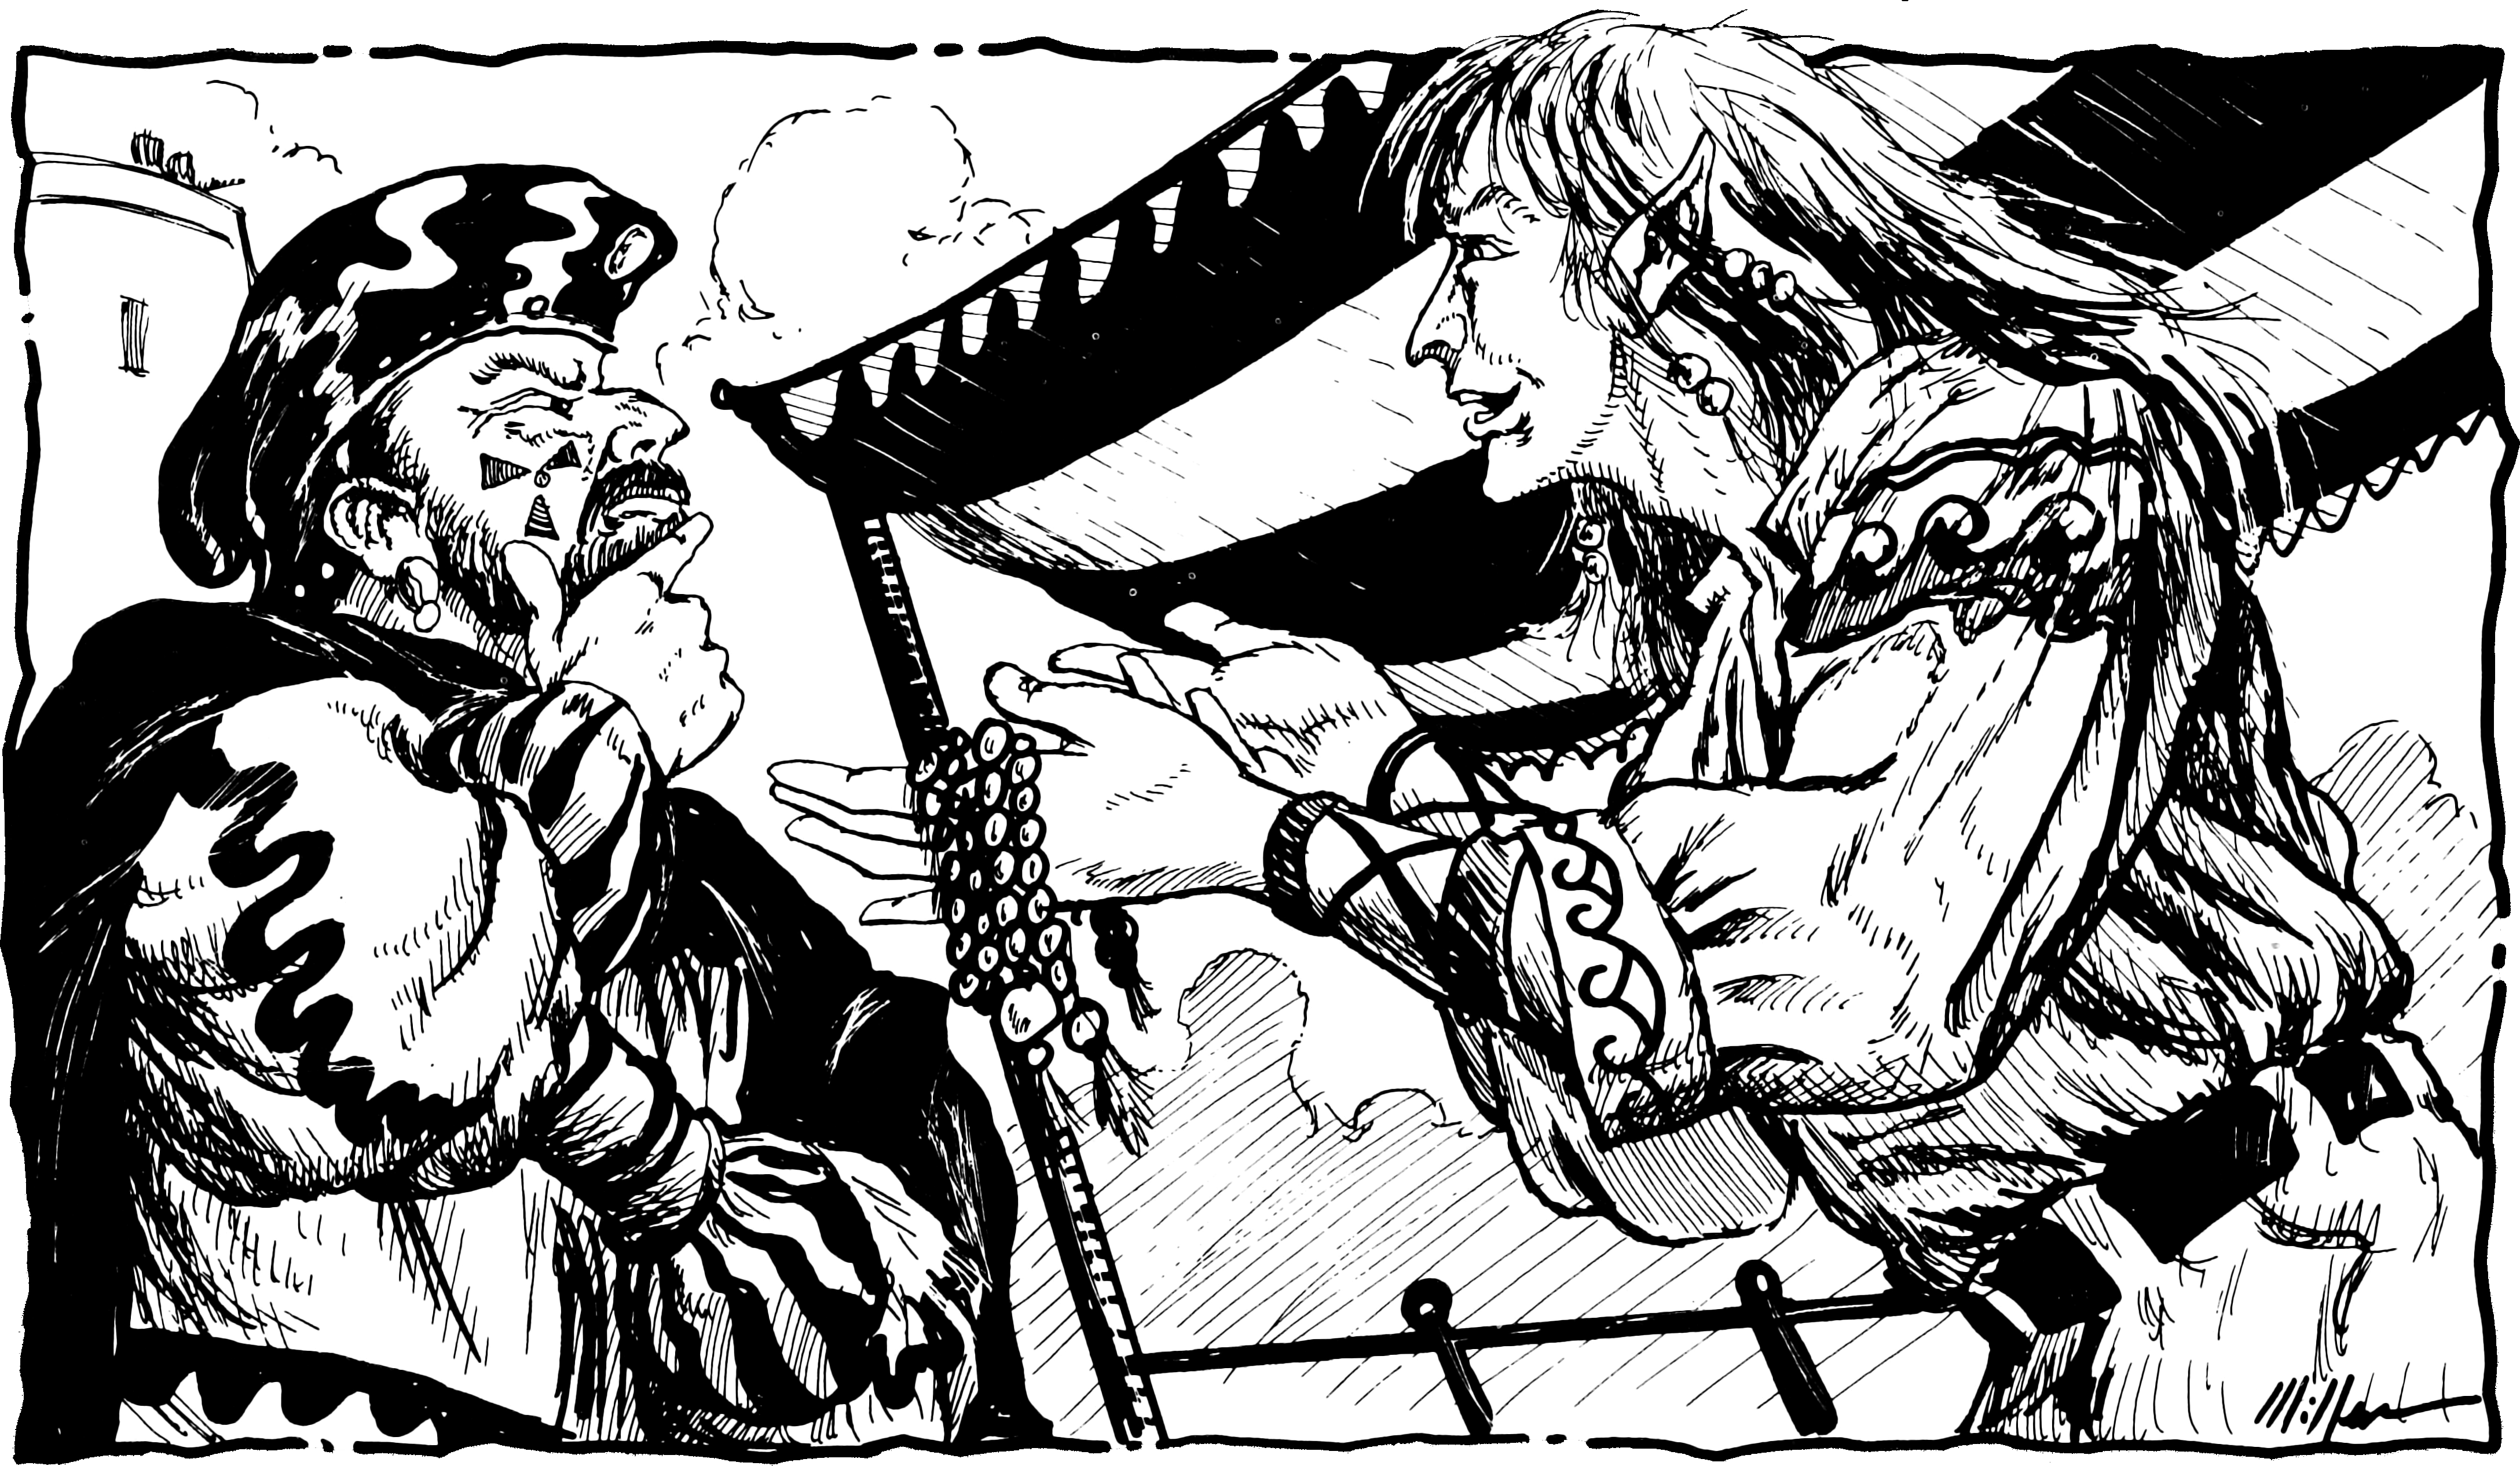
\includegraphics[width=\textwidth]{images/merchant-1.png}
\par\textit{\small\textcopyright Wizards of the Coast, 2020.}
\end{figure*}

\subsection{Adventuring Gear}

\Table{Adventuring Gear}{l RRRR}{
&& \multicolumn{3}{c}{\tableheader Weight}\\
\cmidrule[0.5pt]{3-5}
\tableheader Goods & \tableheader Cost & \tableheader M & \tableheader S & \tableheader L\\
Backpack (empty) & 2 cp & 1 kg & 0.25 kg & 4 kg\\
Barrel (empty) & 2 cp & 15 kg & &\\
Basket (empty) & 4 bits & 0.5 kg & &\\
Bedroll & 1 bits & 2.5 kg & 2.5 kg & 2.5 kg\\
Bell & 1 cp & & &\\
Blanket, winter & 5 bits & 1.5 kg & 0.37 kg & 6 kg\\
Block and tackle & 5 cp & 2.5 kg & &\\
Bottle, wine, glass & 2 cp & & &\\
Bucket (empty) & 5 bits & 1 kg & &\\
Caltrops & 1 cp & 1 kg & &\\
Candle & 1 bd & & &\\
Canvas (sq. m.) & 1 bits & 0.5 kg & &\\
Case, map or scroll & 1 cp & 0.25 kg & &\\
Chain (3 m.) & 30 cp & 1 kg & &\\
Chalk, 1 piece & 1 bd & & &\\
Chest (empty) & 2 cp & 12.5 kg & &\\
Crowbar & 2 cp & 2.5 kg & &\\
Firewood (per day) & 1 bd & 10 kg & &\\
Fishhook & 1 bits & & &\\
Fishing net, 2 sq. m. & 4 cp & 2.5 kg & &\\
Flask (empty) & 3 bd & 0.75 kg & &\\
Flint and steel & 1 cp & & &\\
Grappling hook & 1 cp & 2 kg & &\\
Hammer & 5 bits & 1 kg & &\\
Ink (30 ml vial) & 8 cp & & &\\
Inkpen & 1 bits & & &\\
Jug, clay & 3 bd & 9 lb. & &\\
Ladder, 3-meter & 5 bd & 10 kg & &\\
Lamp, common & 1 bits & 0.5 kg & &\\
Lantern, bullseye & 12 cp & 1.5 kg & &\\
Lantern, hooded & 7 cp & 1 kg & &\\
Lock (very simple) & 20 cp & 0.5 kg & &\\
Lock (average) & 40 cp & 0.5 kg & &\\
Lock (good) & 80 cp & 0.5 kg & &\\
Lock (amazing) & 150 cp & 0.5 kg & &\\
Manacles & 15 cp & 1 kg & &\\
Manacles, masterwork & 50 cp & 1 kg & &\\
Mirror, small steel & 10 cp & 0.25 kg & &\\
Mug/Tankard, clay & 2 bd & 0.5 kg & &\\
Oil (500 ml flask) & 1 bits & 0.5 kg & &\\
Paper (sheet) & 4 bits & & &\\
Parchment (sheet) & 2 bits & & &\\
Pick, miner's & 3 cp & 5 kg & &\\
Pitcher, clay & 2 bd & 2.5 kg & &\\
Piton & 1 bits & 0.25 kg & &\\
Pole, 3-meter & 2 bits & 4 kg & &\\
Pot, iron & 5 bits & 5 kg & &\\
Pouch, belt (empty) & 1 cp & 0.25 kg & 0.06 kg & 1 kg\\
Ram, portable & 10 cp & 10 kg & &\\
Rations, trail (per day) & 5 bits & 0.5 kg & 0.12 kg & 2 kg\\
Rope, giant hair (15 m.) & 50 cp & 5 kg & &\\
Rope, hempen (15 m.) & 1 cp & 5 kg & &\\
Rope, silk (15 m.) & 10 cp & 2.5 kg & &\\
Sack (empty) & 1 bits & 0.25 kg & 0.06 kg & 1 kg\\
Sealing wax & 1 cp & 0.5 kg & &\\
Sewing needle & 5 bits & & &\\
Signal whistle & 8 bits & & &\\
Signet ring & 5 cp & & &\\
Sledge & 1 cp & 5 kg & &\\
Soap (per 0.5 kg) & 5 bits & 0.5 kg & &\\
Spade or shovel & 2 cp & 4 kg & &\\
Spyglass & 1,000 cp & 0.5 kg & &\\
Tent & 10 cp & 10 kg & 2.5 kg & 40 kg\\
Torch & 1 bd & 0.5 kg & &\\
Vial, ink or potion & 1 cp & 0.05 kg & &\\
Waterskin & 1 cp & 2 kg & 0.5 kg & 8 kg\\
Whetstone & 2 bd & 0.5 kg & &\\
}


Some items weight differently for Small or Large characters, these items weigh one-quarter of the Medium-sized when made for Small characters and weigh four times as much the normal weight when made for Large characters. Containers for Small characters also carry one-quarter the normal amount, while containers for Large characters carry four times as much the normal amount.

A few of the pieces of adventuring gear are described below, along with any special benefits they confer on the user (``you'').


\textbf{Caltrops:} A caltrop is a four-pronged iron spike crafted so that one prong faces up no matter how the caltrop comes to rest. You scatter caltrops on the ground in the hope that your enemies step on them or are at least forced to slow down to avoid them. One 1-kilogram bag of caltrops covers an area 1.5 meter square.

Each time a creature moves into an area covered by caltrops (or spends a round fighting while standing in such an area), it might step on one. The caltrops make an attack roll (base attack bonus +0) against the creature. For this attack, the creature's shield, armor, and deflection bonuses do not count. If the creature is wearing shoes or other footwear, it gets a +2 armor bonus to AC. If the caltrops succeed on the attack, the creature has stepped on one. The caltrop deals 1 point of damage, and the creature's speed is reduced by one-half because its foot is wounded. This movement penalty lasts for 24 hours, or until the creature is successfully treated with a DC 15 \skill{Heal} check, or until it receives at least 1 point of magical curing. A charging or running creature must immediately stop if it steps on a caltrop. Any creature moving at half speed or slower can pick its way through a bed of caltrops with no trouble.

Caltrops may not be effective against unusual opponents.

\textbf{Candle:} A candle dimly illuminates a 1.5-meter radius and burns for 1 hour.

\textbf{Chain:} Chain has hardness 10 and 5 hit points. It can be burst with a DC 26 Strength check.

\textbf{Crowbar:} A crowbar grants a +2 circumstance bonus on Strength checks made for such purposes. If used in combat, treat a crowbar as a one-handed improvised weapon that deals bludgeoning damage equal to that of a club of its size.

\textbf{Flint and Steel:} Lighting a torch with flint and steel is a full-round action, and lighting any other fire with them takes at least that long.

\textbf{Grappling Hook:} Throwing a grappling hook successfully requires a \skill{Use Rope} check (DC 10, +2 per 3 meters of distance thrown).

\textbf{Hammer:} If a hammer is used in combat, treat it as a one-handed improvised weapon that deals bludgeoning damage equal to that of a spiked gauntlet of its size.

\textbf{Ink:} This is black ink. You can buy ink in other colors, but it costs twice as much.

\textbf{Jug, Clay:} This basic ceramic jug is fitted with a stopper and holds 4 liters of liquid.

\textbf{Lamp, Common:} A lamp clearly illuminates a 4.5-meter radius, provides shadowy illumination out to a 9-meter radius, and burns for 6 hours on 500 ml of oil. You can carry a lamp in one hand.

\textbf{Lantern, Bullseye:} A bullseye lantern provides clear illumination in a 18-meter cone and shadowy illumination in a 36-meter cone. It burns for 6 hours on 500 ml of oil. You can carry a bullseye lantern in one hand.

\textbf{Lantern, Hooded:} A hooded lantern clearly illuminates a 9-meter radius and provides shadowy illumination in a 18-meter radius. It burns for 6 hours on 500 ml of oil. You can carry a hooded lantern in one hand.

\textbf{Lock:} The DC to open a lock with the \skill{Open Lock} skill depends on the lock's quality: simple (DC 20), average (DC 25), good (DC 30), or superior (DC 40).

\textbf{Manacles and Manacles, Masterwork:} Manacles can bind a Medium creature. A manacled creature can use the \skill{Escape Artist} skill to slip free (DC 30, or DC 35 for masterwork manacles). Breaking the manacles requires a Strength check (DC 26, or DC 28 for masterwork manacles). Manacles have hardness 10 and 10 hit points.

Most manacles have locks; add the cost of the lock you want to the cost of the manacles.

For the same cost, you can buy manacles for a Small creature.

For a Large creature, manacles cost ten times the indicated amount, and for a Huge creature, one hundred times this amount. Gargantuan, Colossal, Tiny, Diminutive, and Fine creatures can be held only by specially made manacles.

\textbf{Oil:} A pint of oil burns for 6 hours in a lantern. You can use a flask of oil as a splash weapon. Use the rules for alchemist's fire, except that it takes a full round action to prepare a flask with a fuse. Once it is thrown, there is a 50\% chance of the flask igniting successfully.

You can pour a pint of oil on the ground to cover an area 1.5 meter square, provided that the surface is smooth. If lit, the oil burns for 2 rounds and deals 1d3 points of fire damage to each creature in the area.

\textbf{Ram, Portable:} This iron-shod wooden beam gives you a +2 circumstance bonus on Strength checks made to break open a door and it allows a second person to help you without having to roll, increasing your bonus by 2.

\textbf{Rope, Giant Hair:} This rope has 5 hardness, 2 hit points and can be burst with a DC 30 Strength check.

\textbf{Rope, Hempen:} This rope has 2 hit points and can be burst with a DC 23 Strength check.

\textbf{Rope, Silk:} This rope has 4 hit points and can be burst with a DC 24 Strength check. It is so supple that it provides a +2 circumstance bonus on \skill{Use Rope} checks.

\textbf{Spyglass:} Objects viewed through a spyglass are magnified to twice their size.

\textbf{Torch:} A torch burns for 1 hour, clearly illuminating a 6-meter radius and providing shadowy illumination out to a 12-meter radius. If a torch is used in combat, treat it as a one-handed improvised weapon that deals bludgeoning damage equal to that of a gauntlet of its size, plus 1 point of fire damage.

\textbf{Vial:} A vial holds 30 milliliters of liquid. The stoppered container usually is no more than 3 centimeters wide and 8 centimeters high.

\subsection{Special Substances And Items}
The following items are often, but not always available for sale in the Bard's Quarter of most city-states. Contacting someone willing to sell these and other associated goods usually requires proficient use of the \skill{Bluff}, \skill{Diplomacy}, and/or \skill{Gather Information} skills.

Any of these substances except for the everburning torch and holy water can be made by a character with the \skill{Craft} (alchemy) skill.

\ItemTable{Special Substances and Items}{
Acid (flask) & 10 cp & 0.5 kg\\
Alchemist's fire (flask) & 20 cp & 0.5 kg\\
Antitoxin (vial) & 50 cp &\\
Balican sting & 5 cp & 0.5 kg\\
Chitin ointment & 40 cp & 0.5 kg\\
Draxia ointment & 20 cp & 0.5 kg\\
Esperweed & 250 cp &\\
Everburning torch & 110 cp & 0.5 kg\\
Holy water (flask) & 25 cp & 0.5 kg\\
Hypnotic brew & 30 cp & 0.5 kg\\
Ignan tallgrass & 100 cp &\\
Kuzza powder & 20 cp &\\
Ranike sap (1 liter) & 2 cp & 0.5 kg\\
Smokestick & 20 cp & 0.25 kg\\
\TableSubheader{Splash-globe}&&\\
~ Acid & 10 cp &\\
~ Kip pheromones & 30 cp &\\
~ Liquid darkness & 10 cp &\\
~ Liquid dust & 10 cp &\\
~ Liquid fire & 10 cp &\\
~ Liquid light & 10 cp &\\
~ Poison & Poison cost $\times$ 1.5 &\\
~ Ranike sap smoke & 10 cp &\\
~ Stench cloud & 50 cp &\\
~ Stun cloud & 35 cp &\\
Sunrod & 2 cp & 0.5 kg\\
Tanglefoot bag & 50 cp & 2 kg\\
Thunderstone & 30 cp & 0.5 kg\\
Tindertwig & 1 cp &\\
}

\textbf{Acid:} You can throw a flask of acid as a splash weapon. Treat this attack as a ranged touch attack with a range increment of 3 meters. A direct hit deals 1d6 points of acid damage. Every creature within 1.5 meter of the point where the acid hits takes 1 point of acid damage from the splash.

\textbf{Alchemist's Fire:} You can throw a flask of alchemist's fire as a splash weapon. Treat this attack as a ranged touch attack with a range increment of 3 meters.

A direct hit deals 1d6 points of fire damage. Every creature within 1.5 meter of the point where the flask hits takes 1 point of fire damage from the splash. On the round following a direct hit, the target takes an additional 1d6 points of damage. If desired, the target can use a full-round action to attempt to extinguish the flames before taking this additional damage. Extinguishing the flames requires a DC 15 Reflex save. Rolling on the ground provides the target advantage on the save. Leaping into a lake or magically extinguishing the flames automatically smothers the fire.

\textbf{Antitoxin:} If you drink antitoxin, you get a +5 alchemical bonus on Fortitude saving throws against poison for 1 hour.

\textbf{Balican Sting:} This mixture of many vegetal irritants is used in conjunction with the flint-tipped javelin of the Balican fleet. Bards working for the late king Andropinis developed the substance to improve the damage done by his warriors fighting against the thick-skinned giants. This mixture, which is only effective against giants of the beasthead, crag, desert, or plains variety, causes the wound made by a balican javelin that breaks within it to itch. Unless a DC 15 Wisdom check is made by the giant on each of the following 1d4 rounds, he will scratch and inadvertently rub the shallow shards deeper, causing an additional 1d4 points of damage for each failed check.

\textbf{Chitin Ointment:} This salve is used to cure damaged chitin on kreens and other insectoid creatures. Once applied, as a standard action, this substance mends brittle or broken chitin, effectively stabilizing the creature if it had less than 0 hit points. Applying this substance to non-chitinous creatures produces no effects.

\textbf{Draxia Ointment:} The draxia weed grows on the islands of the Sea of Silt. It can be turned into an ointment that repels silt spawn by mixing the plant's juices with oil or fat. The ointment, when applied to the skin, emits a smell that repels silt spawn for two hours. Silt spawn will not come within 3 meters of a creature or object coated with draxia ointment. Although adult silt horrors find the smell irritating, they are usually unaffected by it. Sometimes silt horrors are irritated to such a level, however, that they may attack the creature or object giving off the smell. There is a 60\% chance that a silt horror will ignore all other targets and instead attack a character or object that smells of draxia weed.

\textbf{Everburning Torch:} This otherwise normal torch has a continual flame spell cast upon it. An everburning torch clearly illuminates a 6-meter radius and provides shadowy illumination out to a 12-meter radius.

\textbf{Holy Water:} Holy water damages undead creatures and evil outsiders almost as if it were acid. A flask of holy water can be thrown as a splash weapon.

Treat this attack as a ranged touch attack with a range increment of 3 meters. A flask breaks if thrown against the body of a corporeal creature, but to use it against an incorporeal creature, you must open the flask and pour the holy water out onto the target. Thus, you can douse an incorporeal creature with holy water only if you are adjacent to it. Doing so is a ranged touch attack that does not provoke attacks of opportunity.

A direct hit by a flask of holy water deals 2d4 points of damage to an undead creature or an evil outsider. Each such creature within 1.5 meter of the point where the flask hits takes 1 point of damage from the splash.

Temples to good deities sell holy water at cost (making no profit).

\textbf{Ignan Tallgrass:} A redish plant that grows in the Burning Plains near the Last Sea, ignan tallgrass can be harvested from the plains after flashfires, when they are easily spotted in small clumps untouched by the fires. Ignan tallgrass is tough and can be used to make mats and roofs of twinned fibers that stay fireproof for several months, if the harvesters are brave enough to face the flashfires to get to it, as the plant cannot be cultivated. If ignan tallgrass is sun-dried, crushed, and ingested within a week of it being picked, unless somehow magically kept fresh (as through the nurturing seeds spell), it confers resistance to fire 1 for one hour.

\textbf{Kuzza Powder:} Kuzza peppers are very hot. Typically, these vivid red peppers, when ripe, measure 2 to 2 1/2 inches long. These peppers are sometimes dried and ground into a powder by unscrupulous gladiators who use a blowpipe to blow the powder on a target, causing sever irritation. Treat this blowpipe as a blowgun with half the range increment. Filling a blowpipe is a move action that provokes attacks of opportunity. A direct hit blinds a creature for 1 round unless it makes a Fortitude save (DC 15). Every creature within 1.5 meter of the target takes a $-2$ penalty to \skill{Search} and \skill{Spot} checks for 5 rounds.

\textbf{Ranike Sap:} The sap of the ranike tree, which constantly runs down its bark, is toxic to insects. Gulg posesses the secret of safely extracting large quantities of sap from this tree, effectively milking the tree in a process called ``bleeding''. If a liter of the sap is poured in a large receptacle, such as a brazier, and lit afire, a clear smoke that impairs neither vision or breathing forms, filling a 15-meter cube (a moderate or stronger wind dissipates the smoke in 5 rounds). The smoke repels mundane insects, while giant insects, or those creatures that can be categorised as insect-like (such as antloids, kanks, and thri-kreen), that breathe or contact the smoke must make a Fortitude save (DC 15) each round for one minute; failure indicates that they are sickened for that round. The sap burns 1 hour for each liter of sap in the receptacle, after which the smoke dissipates naturally.

A shallow depression in the ground several meters wide can replace the need for a receptacle. The sap can also be used to deliniate an area---each liter poured on the ground can create a line a few inches wide and 3 meters long. When such a line is set afire, it burns for 1 minute and creates smoke in an area 3 meters long by 1.5 meter wide and high.

\textbf{Smokestick:} This alchemically treated wooden stick instantly creates thick, opaque smoke when ignited. The smoke fills a 3-meter cube (treat the effect as a fog cloud spell, except that a moderate or stronger wind dissipates the smoke in 1 round). The stick is consumed after 1 round, and the smoke dissipates naturally.

\textbf{Splash-globes:} Splash-globes are spherical glass jars containing contact poison or up to half a pint of some alchemical fluid. In addition to bursting on impact like any grenade, splash-globes can be placed in hinged pelota, thus giving the grenade additional range when fired through a splash-bow or dejada. The following types of splash-globes are available:

 \textit{Acid:} Standard flask acid can be placed in splash-globes.

 \textit{Contact Poison:} Any contact poison can be placed in a splash-globe.

 \textit{Kip Pheromones:} This splash-globe is commonly crafted by bards using kip pheromones collected by dwarven kip herders. The liquid contained within the globe is an alchemical mixture that turns into smoke on contact with air. The smoke produced is clear and does not impair vision or breathing, filling a 3-meter cube for one minute (a moderate or stronger wind dissipates the smoke in 1 round). Those within the smoke must make a DC 15 Fortitude save each round they are in contact with it or become fascinated for the as long as the smoke remains. Dwarves gain a +4 racial bonus on their Fortitude save against kip pheromones.

 \textit{Liquid Darkness:} Anyone struck directly by liquid darkness must make a Reflex save (DC 15) or be blinded for one minute. Those splashed with liquid darkness have their vision blurred for one minute if they fail a DC 15 Reflex save, granting their opponents concealment. In addition, all natural fires within the splash area are instantly extinguished. Liquid darkness immediately extinguishes liquid light.

 \textit{Liquid Dust:} The liquid from this splash-globe turns into dust on contact with the air. You can use this liquid to cover up to 20 1.5-meter squares of tracks. On impact, liquid dust forms a 4.5-meter diameter cloud, three meters high that lasts one round. Alternately, liquid dust can be launched via slash-globes. Anyone struck directly by liquid dust must make a DC 15 Fortitude save each round for one minute; failure dictates that they are nauseated for that round. Those splashed with liquid dust suffer the same effect for one round if they fail a DC 15 Fortitude save.

 \textit{Liquid Fire:} Alchemist's fire can be placed in splash-globes.

 \textit{Liquid Light:} This splash-globe contains two liquids that mix together when the splash-globe is ruptured. The resulting mixture glows for eight hours. If you break the liquid light globe while it is still in its pouch, the pouch can serve as a light source just like a sunrod. Anyone struck directly by liquid light must make a DC 20 Fortitude save or be temporarily dazzled ($-1$ on all attack rolls) for 1 minute, and will glow in darkness for eight hours unless they somehow cover the affected areas. Creatures splashed with liquid light (see grenade rules) also glow in the darkness, but are not blinded.

 \textit{Ranike Sap Smoke:} The liquid from this splash-globe is an alchemical mixture of ranike sap that turns into smoke on contact with air. The smoke produced is clear and does not impair vision or breathing, filling a 3-meter cube (a moderate or stronger wind dissipates the smoke at the end of the character's action). The smoke repels mundane insects, while giant insects, or those creatures that can be categorised as insect-like (such as antloids, kanks, and thri-kreens), that breath or enter in contact with the smoke must make a DC 15 Fortitude save each round for one minute; failure indicates that they are sickened for that round. This small quantity of sap only reacts with the air for 1 round, after which the smoke dissipates naturally.

 \textit{Stench Cloud:} The liquid inside this splash-globe is crafted from fordorran musk and stinkweed extract. The foul liquid turns into smoke on contact with air. The smoke produced is clear and does not impair vision or breathing, filling a 3-meter cube for one minute (a moderate or stronger wind dissipates the smoke in 1 round). Those within the smoke must make a DC 15 Fortitude save each round they are in contact with it or become nauseated for as long as they remain in contact with the cloud.

 \textit{Stun Cloud:} The liquid inside this splash-globe is crafted from boiled floater jelly combined with the pulped spines from a poisonous cactus. The liquid turns into smoke on contact with air. The smoke produced is clear and does not impair vision or breathing, filling a 3-meter cube for one minute (a moderate or stronger wind dissipates the smoke in 1 round). Those within the smoke must make a DC 15 Fortitude save each round they are in contact with it or become stunned for as long as they remain in contact with the cloud.

\textbf{Sunrod:} This 30-centimeter long, gold-tipped, iron rod glows brightly when struck. It clearly illuminates a 9-meter radius and provides shadowy illumination in a 18-meter radius. It glows for 6 hours, after which the gold tip is burned out and worthless.

\textbf{Tanglefoot Bag:} When you throw a tanglefoot bag at a creature (as a ranged touch attack with a range increment of 3 meters), the bag comes apart and the goo bursts out, entangling the target and then becoming tough and resilient upon exposure to air. An entangled creature takes a $-2$ penalty on attack rolls and a $-4$ penalty to Dexterity and must make a DC 15 Reflex save or be glued to the floor, unable to move. Even on a successful save, it can move only at half speed. Huge or larger creatures are unaffected by a tanglefoot bag. A flying creature is not stuck to the floor, but it must make a Reflex save (DC 15) or be unable to fly (assuming it uses its wings to fly) and fall to the ground. A tanglefoot bag does not function underwater.

A creature that is glued to the floor (or unable to fly) can break free by making a DC 17 Strength check or by dealing 15 points of damage to the goo with a slashing weapon. A creature trying to scrape goo off itself, or another creature assisting, does not need to make an attack roll; hitting the goo is automatic, after which the creature that hit makes a damage roll to see how much of the goo was scraped off. Once free, the creature can move (including flying) at half speed. A character capable of spellcasting who is bound by the goo must make a \skill{Concentration} check (DC 15) to cast a spell. The goo becomes brittle and fragile after 2d4 rounds, cracking apart and losing its effectiveness. An application of universal solvent to a stuck creature dissolves the alchemical goo immediately.

\textbf{Thunderstone:} You can throw this stone as a ranged attack with a range increment of 6 meters. When it strikes a hard surface (or is struck hard), it creates a deafening bang that is treated as a sonic attack. Each creature within a 3-meter-radius spread must make a DC 15 Fortitude save or be deafened for 1 hour. A deafened creature, in addition to the obvious effects, takes a $-4$ penalty on initiative and has a 20\% chance to miscast and lose any spell with a verbal component that it tries to cast.

Since you don't need to hit a specific target, you can simply aim at a particular 1.5-meter square. Treat the target square as AC 5.

\textbf{Tindertwig:} The alchemical substance on the end of this small, wooden stick ignites when struck against a rough surface. Creating a flame with a tindertwig is much faster than creating a flame with flint and steel (or a magnifying glass) and tinder. Lighting a torch with a tindertwig is a standard action (rather than a full-round action), and lighting any other fire with one is at least a standard action.
\subsectionA{Metaempiric Components}
Useful for spellcasters, these items are special material components that have a chance of influencing the casting of certain spells while held in hand. Since a metempiric component must be held in one hand to use, it cannot be used in conjunction with the \feat{Still Spell} feat and, being optional for the casting of a spell, does not count as a normal material component for the purpose of the \feat{Eschew Materials} feat. Metempiric components are consumed during the casting of a spell, unless otherwise noted.

\ItemTable{Metaempiric Components}{
Aviarag horn & 1,350 cp & 2.5 kg\\
Beasthead blood & 45 cp & 0.5 kg\\
Dagorran crystal, diminutive & 100 cp &\\
Dagorran crystal, tiny & 300 cp & 0.25 kg\\
Defiler's ash & 1,700 cp &\\
Defiled poisonweed petals & 350 cp &\\
Eagle beasthead feather & 40 cp &\\
Roc feather & 450 cp &\\
Royal justice token & 1,375 cp & 0.5 kg\\
Shadow giant fumes & 390 cp & 0.5 kg\\
Sun paraelemental essence & 935 cp & 0.5 kg\\
T'chowb's thalamus & 1,250 cp & 0.25 kg\\
}

\textbf{Aviarag Horn:} A horn willingly given by an aviarag for use by someone after its passing into death is a powerful weapon for those seeking to do good. When presented while casting a spell, the goodness still emanating from the beast's horn is so tangible that the spell itself benefits from it. When used as a component for any spell with the good descriptor, the aviarag horn increases the spell's effective caster level by 1d4. An aviarag horn is not consumed after being used.

\textbf{Beasthead Blood:} As sorcerous mutations of normal Athasian giants, the blood of beasthead giants has some magical properties. When beasthead blood is used as a component in any transmutation spell, it increases the spell's saving throw DC by +1. Inexplicably, only druids and preservers may use beasthead blood this way; it provides no benefit for other types of spellcasters.

\textbf{Dagorran Crystal:} This green crystal growth is extracted from the body of a daggoran. Daggorans come in two sizes, which affect the size and potency of the crystal: a Medium daggoran provides a Diminutive crystal while a Large daggoran provides a Tiny crystal. When used as a component for a spell with the mind-affecting descriptor, a Diminutive daggoran crystal increases the spell's saving throw DC by +2.

\textbf{Defiler's Ash:} Mixed in with a special mixture of blood, these ashes must be taken from at least three different spellcasters' ashen circles caused by powerful spellcasting (spell level 6th and above). When used in the casting of a spell with the necromancy descriptor, defiler's ash empower the spell as if the caster had applied the Empower Spell feat (but without changing the spell's effective level or increasing its casting time).

\textbf{Defiled Poisonweed Petals:} The bright orange petals of a poisonweed plant turned undead by the action of defiling represent the epitome of noxiousness. When used as a component for any spell with the death descriptor, the petals of a defiled poisonweed increase the spell's saving throw DC by +2.

\textbf{Eagle Beasthead Feather:} If a feather from an eagle-headed beasthead giant is in hand when falling, it can be used as a component when casting feather fall, doubling the duration of the spell.

\textbf{Roc Feather:} These huge feathers---from anywhere between 0.6 and 1.2 meter long---come from an Athasian rock. When used as a component for a spell confering flight, a roc feather doubles the spell's duration.

\textbf{Royal Justice Token:} Only used by templars in the service of the sorcerer-monarch for which the token was created, the royal justice token shows graven symbols associated with the justice system used in a particular city-state. Symbols include ever-vigilant eyes, readied swords, and open hand or closed fist. When used as a component for the \spell{wrath of the sorcerer-king} spell, the token increases the spell's effective caster level by +2. A royal justice token is not consumed after being used.

\textbf{Shadow Giant Fumes:} If bottled, the black, cold fumes that emanate from a shadow giant's mouth as it speaks can be used to enhance spells that have a connection to the Black. When used as a component for the spells \spell{greater shadow conjuration}, \spell{shades}, or \spell{shadow conjuration}, the potency of the spell is one-fifth (20\%) better than normal.

\textbf{Sun Paraelemental Essence:} This bright and blinding essence comes from a dead sun paraelemental of at least Huge size. The essence must be trapped in a clear crystal container within one minute of the elemental's death and must always be kept under the light of the sun during the day, or else losing its potency. During the night, the light fades and gives off the same illumination as a candle. When used as a component for any spell with the light descriptor, the essence increases the effective caster level by +2.

\textbf{T'chowb's Thalamus:} The thalamus of a recently fed (within the last 24 hours) t'chowb is said to be seething with absorbed intelligence. When used as a metempiric component, the t'chowb's thalamus gives the caster a +10 circumstance bonus on caster level checks made to overcome a target's spell resistance.
\subsection{Psychoactive Components}
Useful for manifesters, these items are components that have a chance of influencing the manifestation of certain powers when used properly. Unlike metempiric components, each psychoactive component must be used in a specific fashion in order to provide its benefits to the manifester. Unless otherwise noted, psychoactive components are consumed during the manifesting of a power.

Also included in this category is a creature sometimes used by psionic characters to access the residual psionic energy their mind's produce throughout the day.

\ItemTable{Psychoactive Components}{
Aviarag horn melange & 250 cp & 0.5 kg\\
Bouyan crystal & 400 cp & 1 kg\\
Cilops compound eye & 65 cp & \\
Dagorran crystal, diminutive & 100 cp & \\
Dagorran crystal, tiny & 300 cp & \onequarter kg\\
Tas'l worm & 100 cp & \\
T'chowb's thalamus & 1,250 cp & \onequarter kg\\
}

\textbf{Aviarag Horn Melange:} The great horn of the noble aviarag, when crushed and mixed with a specially treated wine, preserves some of the psionic power of the aviarag and can expand the reach and power of the drinker's mind. A manifester drinking this psychoactive substance no more than 1 minute before using the \psionic{mindwipe} power increases the power's save DC by +2, and drinking it before manifesting \psionic{mindlink} doubles the power's range, as per the \feat{Enlarge Power} feat (but without changing the power's effective level or requiring the expendature of a psionic focus). Drinking this melange is a standard action that provokes attacks of opportunity.

\textbf{Bouyan Crystal:} From salt formations found within the great salt plains, the clear gray bouyan stone is cut to a great degree of perfection, allowing a manifester to focus his mind upon it. A manifester that concentrates upon a held bouyan crystal when manifesting any telepathy power (a free action, assuming the manifester is already holding the component) increases the power's effective manifester level by +1.

\textbf{Cilops Compound Eye:} Crushing the central compound eye of a cilops produces a thick jelly that may extend the user's senses of his surroundings. If this jelly is spread over the eyes of a character (a full-round action) before he manifests object reading, and the temporary blindness it induces is endured for the extent of the power's duration, then this power always successfully identifies all other former owners of an object in sequence, with no chance that former owners will be skipped and thus not identified. Removing the jelly from one's eyes, thus negating the blindness, takes 1 minute. Eating the jelly before manifesting sensitivity to psychic impressions reduces the manifesting time of that power to 10 minutes.

\textbf{Dagorran Crystal:} This green crystal growth is extracted from the body of a daggoran. Manifesters use these crystals to harness the dagorran's ability to sense the psionic nature of creatures. A Diminutive daggoran crystal gives manifesters advantage to \skill{Psicraft} checks made when using the \psionic{psychic tracking} psionic power, while a Tiny daggoran crystal gives a +5 competence bonus. Such a crystal is not consumed when used.

\textbf{Tas'l Worm:} Tas'l worms are worms of Diminutive size, similar in appearance to ock'n, but without eyestalks. Only found on living psionic creatures, these 1-inch long worms snake slowly between the skin and the skull of their host, accumulating and living off of residual psionic energy.

A tas'l worm can be removed by cutting open the skin. A character can remove a worm by taking 10 minutes to locate and extract it from the host's scalp. The extraction does 1d6 points of damage to the victim, and has a 75\% chance of killing the worm in the process. If a successful \skill{Heal} check (DC 20) is made, the cutting damage is reduced to 1d2, with no chance of killing the worm.

A worm outside of its host lives for 1 hour. The worm, when put against the skin of a psionic creature, burrows into its flesh, causing 1 point of damage. Afterwards, the worm must stay within the host for at least 24 hours before it amasses enough residual energy to be used. Tas'l worms use the innocuous vermin statistics (see page 191 of Terrors of Athas). A worm linked to a host has a lifespan of 2d6 months. If more than one worm live on the same scalp, there is a 55\% chance for 1d2 worms to spawn each month thereafter.

The creature hosting tas'l worms can make a \skill{Concentration} check (DC 20) as a free action, once per day, to tap the energy they contain. If the check is successful, each tas'l worm hosted by a creature provides 1 power point. All worms must be tapped at once, or none at all. These power points are considered a part of the creature's own power point reserve for the purpose of using stored power points. A failed check can be retried on the character's next turn.

The hosting creature receives a cumulative $-1$ circumstance penalty to Will saves against telepathic powers for each worm living within its body, as the worms make their host more responsive to outside psionic influence.

A tas'l worm registers as psionic to \psionic{detect psionics}.

\textbf{T'chowb's Thalamus:} The thalamus of a recently fed (within the last 24 hours) t'chowb is said to be seething with absorbed intelligence. If crushed in one's hand during the manifestation of a power (a free action, assuming the manifester is already holding the component), the t'chowb's thalamus gives a manifester a +10 circumstance bonus on manifester level checks made to overcome a target's power resistance.
\subsectionA{Tools and Skill Kits}

\ItemTable{Tools and Skill Kits}{
Alchemist's lab & 500 cp & 20 kg\\
Artisan's tools & 5 cp & 2.5 kg\\
Artisan's tools, masterwork & 55 cp & 2.5 kg\\
Book of poisons & 125 cp & 1 kg\\
Candle of rejuvenation & 50 cp & \\
Climber's kit & 80 cp & 2.5 kg1\\
Concealing weave & 5 cp & 1 kg\\
Disguise kit & 50 cp & 4 kg1\\
Healer's kit & 50 cp & 0.5 kg\\
Holly and mistletoe & & \\
Holy symbol, silver & 25 cp & 0.5 kg\\
Holy symbol, wooden & 1 cp & \\
Hourglass & 25 cp & 0.5 kg\\
Magnifying glass & 100 cp & \\
Meditative kit & 35 cp & 1.5 kg\\
Musical instrument, common & 5 cp & 1.5 kg1\\
Musical instrument, masterwork & 100 cp & 1.5 kg1\\
Navigator kit & 75 cp & 5 kg\\
Remote viewing kit & & 5 kg\\
Scale, merchant's & 2 cp & 0.5 kg\\
Spell component pouch & 5 cp & 1 kg\\
Spellbook, wizard's (blank) & 15 cp & 1.5 kg\\
Thieves' tools & 30 cp & 0.5 kg\\
Thieves' tools, masterwork & 100 cp & 1 kg\\
Tool, masterwork & 50 cp & 0.5 kg\\
Water clock & 1,000 cp & 100 kg\\
}

The items described below are particularly useful to characters that have certain specific skills or abilities and are used in specific situations.


\textbf{Alchemist's Lab:} An alchemist's lab always has the perfect tool for making alchemical items, so it provides +2 circumstance bonus on \skill{Craft} (alchemy) checks. It has no bearing on the costs related to the \skill{Craft} (alchemy) skill. Without this lab, a character with the \skill{Craft} (alchemy) skill is assumed to have enough tools to use the skill but not enough to get the +2 bonus that the lab provides.

\textbf{Artisan's Tools, Masterwork:} These tools serve the same purpose as artisan's tools (above), but masterwork artisan's tools are the perfect tools for the job, so you get +2 circumstance bonus on \skill{Craft} checks made with them.

\textbf{Artisan's Tools:} These special tools include the items needed to pursue any craft. Without them, you have to use improvised tools (-2 penalty on \skill{Craft} checks), if you can do the job at all.

\textbf{Book of Poisons:} The original Book of Poisons is rumored to have been written by the half-elven bard Cabal, with current copies containing but fragments of the original poison recipes. This set of clay tablets is covered with markings, known mostly to bards, that can only be understood by making a \skill{Decipher Script} check (DC 15). Once deciphered, the reader can see that they contain a number of recipes that describe, step-by-step, tried-and-true methods for crafting specific poisons. The tablets grant the following benefits when used in conjunction with the crafting of poisons described in the set (normally 5 to 10 different poisons, of the DM's choice): +2 circumstance bonus to \skill{Craft} (poisonmaking) checks and a +1 to the save DC of the poisons being crafted. This last bonus stacks with the scorpion's touch bardic ability.

\textbf{Candle of Rejuvenation:} This item allows a manifester to recover power points as if he were resting at night. The manifester recovers 10 power points at the end of each complete hour spent within 3 meters of a lit candle. By making an \skill{Autohypnosis} DC 15 check, this amount increases by one-half. Each candle burns for a total of eight hours.

\textbf{Climber's Kit:} This is the perfect tool for climbing and gives you +2 circumstance bonus on \skill{Climb} checks.

\textbf{Concealing Weave:} This kit is composed of one or more related articles of clothing specifically made to camouflage a caster's arm and hand movements while casting a spell. This kit grants +2 circumstance bonus on \skill{Bluff} checks made to conceal the casting of spells with a somatic component.

\textbf{Disguise Kit:} The kit is the perfect tool for disguise and provides +2 circumstance bonus on \skill{Disguise} checks. A disguise kit is exhausted after ten uses.

\textbf{Healer's Kit:} It is the perfect tool for healing and provides +2 circumstance bonus on \skill{Heal} checks. A healer's kit is exhausted after ten uses.

\textbf{Holy Symbol, Silver or Wooden:} A holy symbol focuses positive energy. A cleric uses it as the focus for his spells and as a tool for turning undead. Each religion has its own holy symbol.

 \textit{Unholy Symbols:} An unholy symbol is like a holy symbol except that it focuses negative energy and is used by evil clerics (or by neutral clerics who want to cast evil spells or command undead).

 \textit{Sorcerer-king's Sigil:} A sorcerer-king's sigil is like a holy symbol for templars. It is the sign of their rank and station within the templarate. It is unique to each city-state.

\textbf{Magnifying Glass:} This simple lens allows a closer look at small objects. It is also useful as a substitute for flint and steel when starting fires. Lighting a fire with a magnifying glass requires light as bright as sunlight to focus, tinder to ignite, and at least a full-round action. A magnifying glass grants +2 circumstance bonus on \skill{Appraise} checks involving any item that is small or highly detailed.

\textbf{Meditative Kit:} This small and delicately carved crystal container produces an hypnotic rainbow-like effect while filled with clear water and struck by light. After 1 minute of uninterrupted observation of the rainbow pattern, the kit provides +2 circumstance bonus to the next \skill{Autohypnosis} check made by the viewer within the next 10 minutes.

\textbf{Musical Instrument, Common or Masterwork:} A masterwork instrument grants +2 circumstance bonus on \skill{Perform} checks involving its use.

\textbf{Navigator's Kit:} Prized posessions of many trading houses and frequent wanderers of the wastes, each of these kits is composed of a set of maps made of straight sticks representing roads, and small stones for villages, cities and others special locations, all lashed together by strings. If you succeed at a \skill{Knowledge} (geography) check DC 10 while using this kit, you gain a +4 bonus on \skill{Survival} checks made to keep from getting lost.

\textbf{Remote Viewing Kit:} This kit allows for a more potent use of the \psionic{remote viewing} power. Unlike other class or skill kits, this kit is created from local natural materials, effectively making it free in cost, but its user must recreate the kit before each use. Five ranks in \skill{Knowledge} (psionics), and 10 minutes, are required to create the kit. It must be created in silence, without distractions, and in a windless area. The kit takes the form of a 1.5-meter square patch of flat ground, covered with sand or particulate dirt to a depth of at least 2.5 centimeters, with 1d6 palm-sized stones deposited on it. Lines and circles are then traced around the stones and over the entire surface, creating a unique, maze-like pattern.

To gain the benefits of the kit, the user must focus on the patch of ground and succeed at a DC 15 \skill{Concentration} check after its creation; failure indicating that the user needs to recreate the kit anew. A successful check means the user's next manifestation of remove viewing, which must be within 1 minute of making the check, is altered in the following ways. First, the subject of the user's viewing attempt receives a $-2$ penalty to his Will saving throw against the \psionic{remote viewing}. Second, the user receives +2 circumstance bonus to \skill{Concentration} checks made to manifest a power through \psionic{remote viewing}. Finally, the user receives +2 circumstance bonus to \skill{Hide} checks to prevent his quasi-real viewpoint from being noticed by the subject he his viewing.

The effects of this kit can be made more potent if more than one character assists with its creation. Each character that helps adds another 1.5-meter square to the space taken by the kit, and another 10 minutes to the time required for the kit's completion. Each character that succeeds at a DC 15 \skill{Concentration} check at the time of the kit's completion can use the aid another action to help the user with skill checks made while the user is manifesting \psionic{remote viewing}. A kit created in this fashion is more complex, and as such requires two more ranks in \skill{Knowledge} (psionics) to create for each additional character that helped in its creation. Only a limited number of characters can help to create a remove viewing kit, equal to half the user's manifester level.

\textbf{Scale, Merchant's:} A scale grants +2 circumstance bonus on \skill{Appraise} checks involving items that are valued by weight, including anything made of precious metals.

\textbf{Spell Component Pouch:} A spellcaster with a spell component pouch is assumed to have all the material components and focuses needed for spellcasting, except for those components that have a specific cost, divine focuses, and focuses that wouldn't fit in a pouch.

\textbf{Spellbook, Wizard's (Blank):} A spellbook has 100 pages of parchment, and each spell takes up one page per spell level (one page each for 0-level spells).

\textbf{Thieves' Tools, Masterwork:} This kit contains extra tools and tools of better make, which grant +2 circumstance bonus on \skill{Disable Device} and \skill{Open Lock} checks.

\textbf{Thieves' Tools:} This kit contains the tools you need to use the \skill{Disable Device} and \skill{Open Lock} skills. Without these tools, you must improvise tools, and you have disadvantage on \skill{Disable Device} and \skill{Open Lock} checks.

\textbf{Tool, Masterwork:} This well-made item is the perfect tool for the job. It grants +2 circumstance bonus on a related skill check (if any). Bonuses provided by multiple masterwork items used toward the same skill check do not stack.

\textbf{Water Clock:} This large, bulky contrivance gives the time accurate to within half an hour per day since it was last set. It requires a source of water, and it must be kept still because it marks time by the regulated flow of droplets of water.
\subsection{Clothing}
Clothes weigh one-quarter the normal amount when made for Small characters, and four times as much when made for Large characters.

\Table{Clothing}{lRRRR}{
&& \multicolumn{3}{c}{\tableheader Weight}\\
\cmidrule[0.25pt]{3-5}
\tableheader Item & \tableheader Cost & \tableheader S & \tableheader M & \tableheader L\\
Artisan's outfit & 1 cp & 0.5 kg & 2 kg & 8 kg\\
Cleric's vestments & 5 cp & 0.75 kg & 3 kg & 12 kg\\
% Cold weather outfit & 8 cp & 3.5 kg & 3.5 kg & 15 kg\\
Courtier's outfit & 30 cp & 0.75 kg & 3 kg & 12 kg\\
Elven outfit & 30 cp & 0.62 kg & 2.5 kg & 10 kg\\
Entertainer's outfit & 3 cp & 0.5 kg & 2 kg & 8 kg\\
Explorer's outfit & 10 cp & 1 kg & 4 kg & 16 kg\\
High templar's outfit & 100 cp & 0.62 kg & 2.5 kg & 10 kg\\
% Monk's outfit & 5 cp & 1 kg & 1 kg & 1 kg\\
Noble's outfit & 75 cp & 1.25 kg & 5 kg & 20 kg\\
Peasant's outfit & 1 sp & 0.25 kg & 1 kg & 4 kg\\
Royal defiler's outfit & 80 cp & 0.62 kg & 2.5 kg & 10 kg\\
Royal outfit & 200 cp & 1.87 kg & 7.5 kg & 30 kg\\
Scholar's outfit & 5 cp & 0.75 kg & 3 kg & 12 kg\\
Slave's outfit & 2 bd & 0.12 kg & 0.5 kg & 2 kg\\
Traveler's outfit & 1 cp & 0.62 kg & 2.5 kg & 10 kg\\
Wastelander outfit & 20 cp & 0.75 kg & 3 kg & 12 kg\\
}


\textbf{Artisan's Outfit:} This outfit includes a shirt with buttons, a skirt or pants with a drawstring, shoes, and perhaps a cap or hat. It may also include a belt or a leather or cloth apron for carrying tools.

\textbf{Cleric's Vestments:} These ecclesiastical clothes are for performing priestly functions, not for adventuring.

% \textbf{Cold Weather Outfit:} A cold weather outfit includes a wool coat, linen shirt, wool cap, heavy cloak, thick pants or skirt, and boots. This outfit grants a +5 circumstance bonus on Fortitude saving throws against exposure to cold weather.

\textbf{Courtier's Outfit:} This outfit includes fancy, tailored clothes in whatever fashion happens to be the current style in the courts of the nobles. Anyone trying to influence nobles or courtiers while wearing street dress will have a hard time of it (-2 penalty on Charisma-based skill checks to influence such individuals). If you wear this outfit without jewelry (costing an additional 50 cp), you look like an out-of-place commoner.

\textbf{Elven Outfit:} Although varying greatly from tribe to tribe, all elven clothing is based around two concepts: functionality and flattery. This set of clothes most often includes a hooded cloak or stylized robes, although some outfits make do with tight leather wrappings or other heat-shielding and water-retaining materials. In regards to its other aspect---visual appeal---every elven outfit is, no matter how functional, also designed to complement the wearer's form. Each outfit is tailor-made by elves, following a particular tribal pattern, and are normally not for sale. In addition, various portions of this outfit---such as a cloak, thick shoulder scarf, or even an entire tunic---are colored, patterned, or designed to be reversible in such a way as to blend in with the Athasian landscape, helping the wearer to blend in with the terrain in sandy areas: this provides a +3 circumstance bonus on \skill{Hide} checks while in desert terrain. For twice the listed price, this outfit can be made to fit over light armor.

\textbf{Entertainer's Outfit:} This set of flashy, perhaps even gaudy, clothes is for entertaining. While the outfit looks whimsical, its practical design lets you tumble, dance, walk a tightrope, or just run (if the audience turns ugly).

\textbf{Explorer's Outfit:} This is a full set of clothes for someone who never knows what to expect. It includes sturdy boots, leather breeches or a skirt, a belt, a shirt (perhaps with a vest or jacket), gloves, and a cloak. Rather than a leather skirt, a leather overtunic may be worn over a cloth skirt. The clothes have plenty of pockets (especially the cloak). The outfit also includes any extra items you might need, such as a scarf or a wide-brimmed hat.

\textbf{High Templar's Outfit:} High templar's outfits differ for each of the Tablelands' cities. This set of clothing is made of the best material produced by a city-state's artisans and exemplifies that city's templarate. Wearing the proper high templar outfit for a city's templarate gives a +2 circumstance bonus to \skill{Diplomacy} checks in contests of the \feat{Secular Authority} feat made within that city.

% \textbf{Monk's Outfit:} This simple outfit includes sandals, loose breeches, and a loose shirt, and is all bound together with sashes. The outfit is designed to give you maximum mobility, and it's made of high-quality fabric. You can hide small weapons in pockets hidden in the folds, and the sashes are strong enough to serve as short ropes.

\textbf{Noble's Outfit:} This set of clothes is designed specifically to be expensive and to show it. Precious metals and gems are worked into the clothing. To fit into the noble crowd, every would-be noble also needs a signet ring (see Adventuring Gear, above) and jewelry (worth at least 100 cp).

\textbf{Peasant's Outfit:} This set of clothes consists of a loose shirt and baggy breeches, or a loose shirt and skirt or overdress. Cloth wrappings are used for shoes.

\textbf{Royal Defiler's Outfit:} Royal defilers, who practice sorcery with the full legal backing of a sorcerer-king, must clearly indicate their protected status if they are to be spared the mob's wrath. This set of clothing is made from the best materials available to a city-state's artisans, and is second in quality only to a templar's outfit. The outfit varies greatly from city to city. In Raam, for example, this outfit is a checkered silk robe adorned with a silver brooch denoting royal defiler status. Wearing the proper defiler outfit for a city gives a +2 circumstance bonus to \skill{Intimidate} checks against citizens who aren't part of the templarate.

\textbf{Royal Outfit:} This is just the clothing, not the royal scepter, crown, ring, and other accoutrements. Royal clothes are ostentatious, with gems, gold, silk, and fur in abundance.

\textbf{Scholar's Outfit:} Perfect for a scholar, this outfit includes a robe, a belt, a cap, soft shoes, and possibly a cloak.

\textbf{Slave's Outfit:} This simple set of clothes consists of a loincloth, or a short skirt and sleeveless tunic, all made of rough-hewn materials.

\textbf{Traveler's Outfit:} This set of clothes consists of boots, a wool skirt or breeches, a sturdy belt, a shirt (perhaps with a vest or jacket), and an ample cloak with a hood.

\textbf{Wastelander's Outfit:} Similar to clothing worn by the many elven tribes dotting the Athasian landscape, this set of clothes commonly includes a large hooded cloak, multiple layers of heat-resistant, porous cloth, and reinforced leather padding designed to protect against blowing sand, sharp rocks and the ever-present cacti needles. In addition, this outfit is colored to blend in with whatever environment the wastelander has chosen as his home, helping the wearer to blend in with rocky surroundings. This provides a +2 circumstance bonus on \skill{Hide} checks while in the appropriate terrain; each wastelander's outfit provides this bonus for a single terrain type only. For twice the price, this outfit can be made to fit over light armor.
\begin{figure*}[b!]
\centering
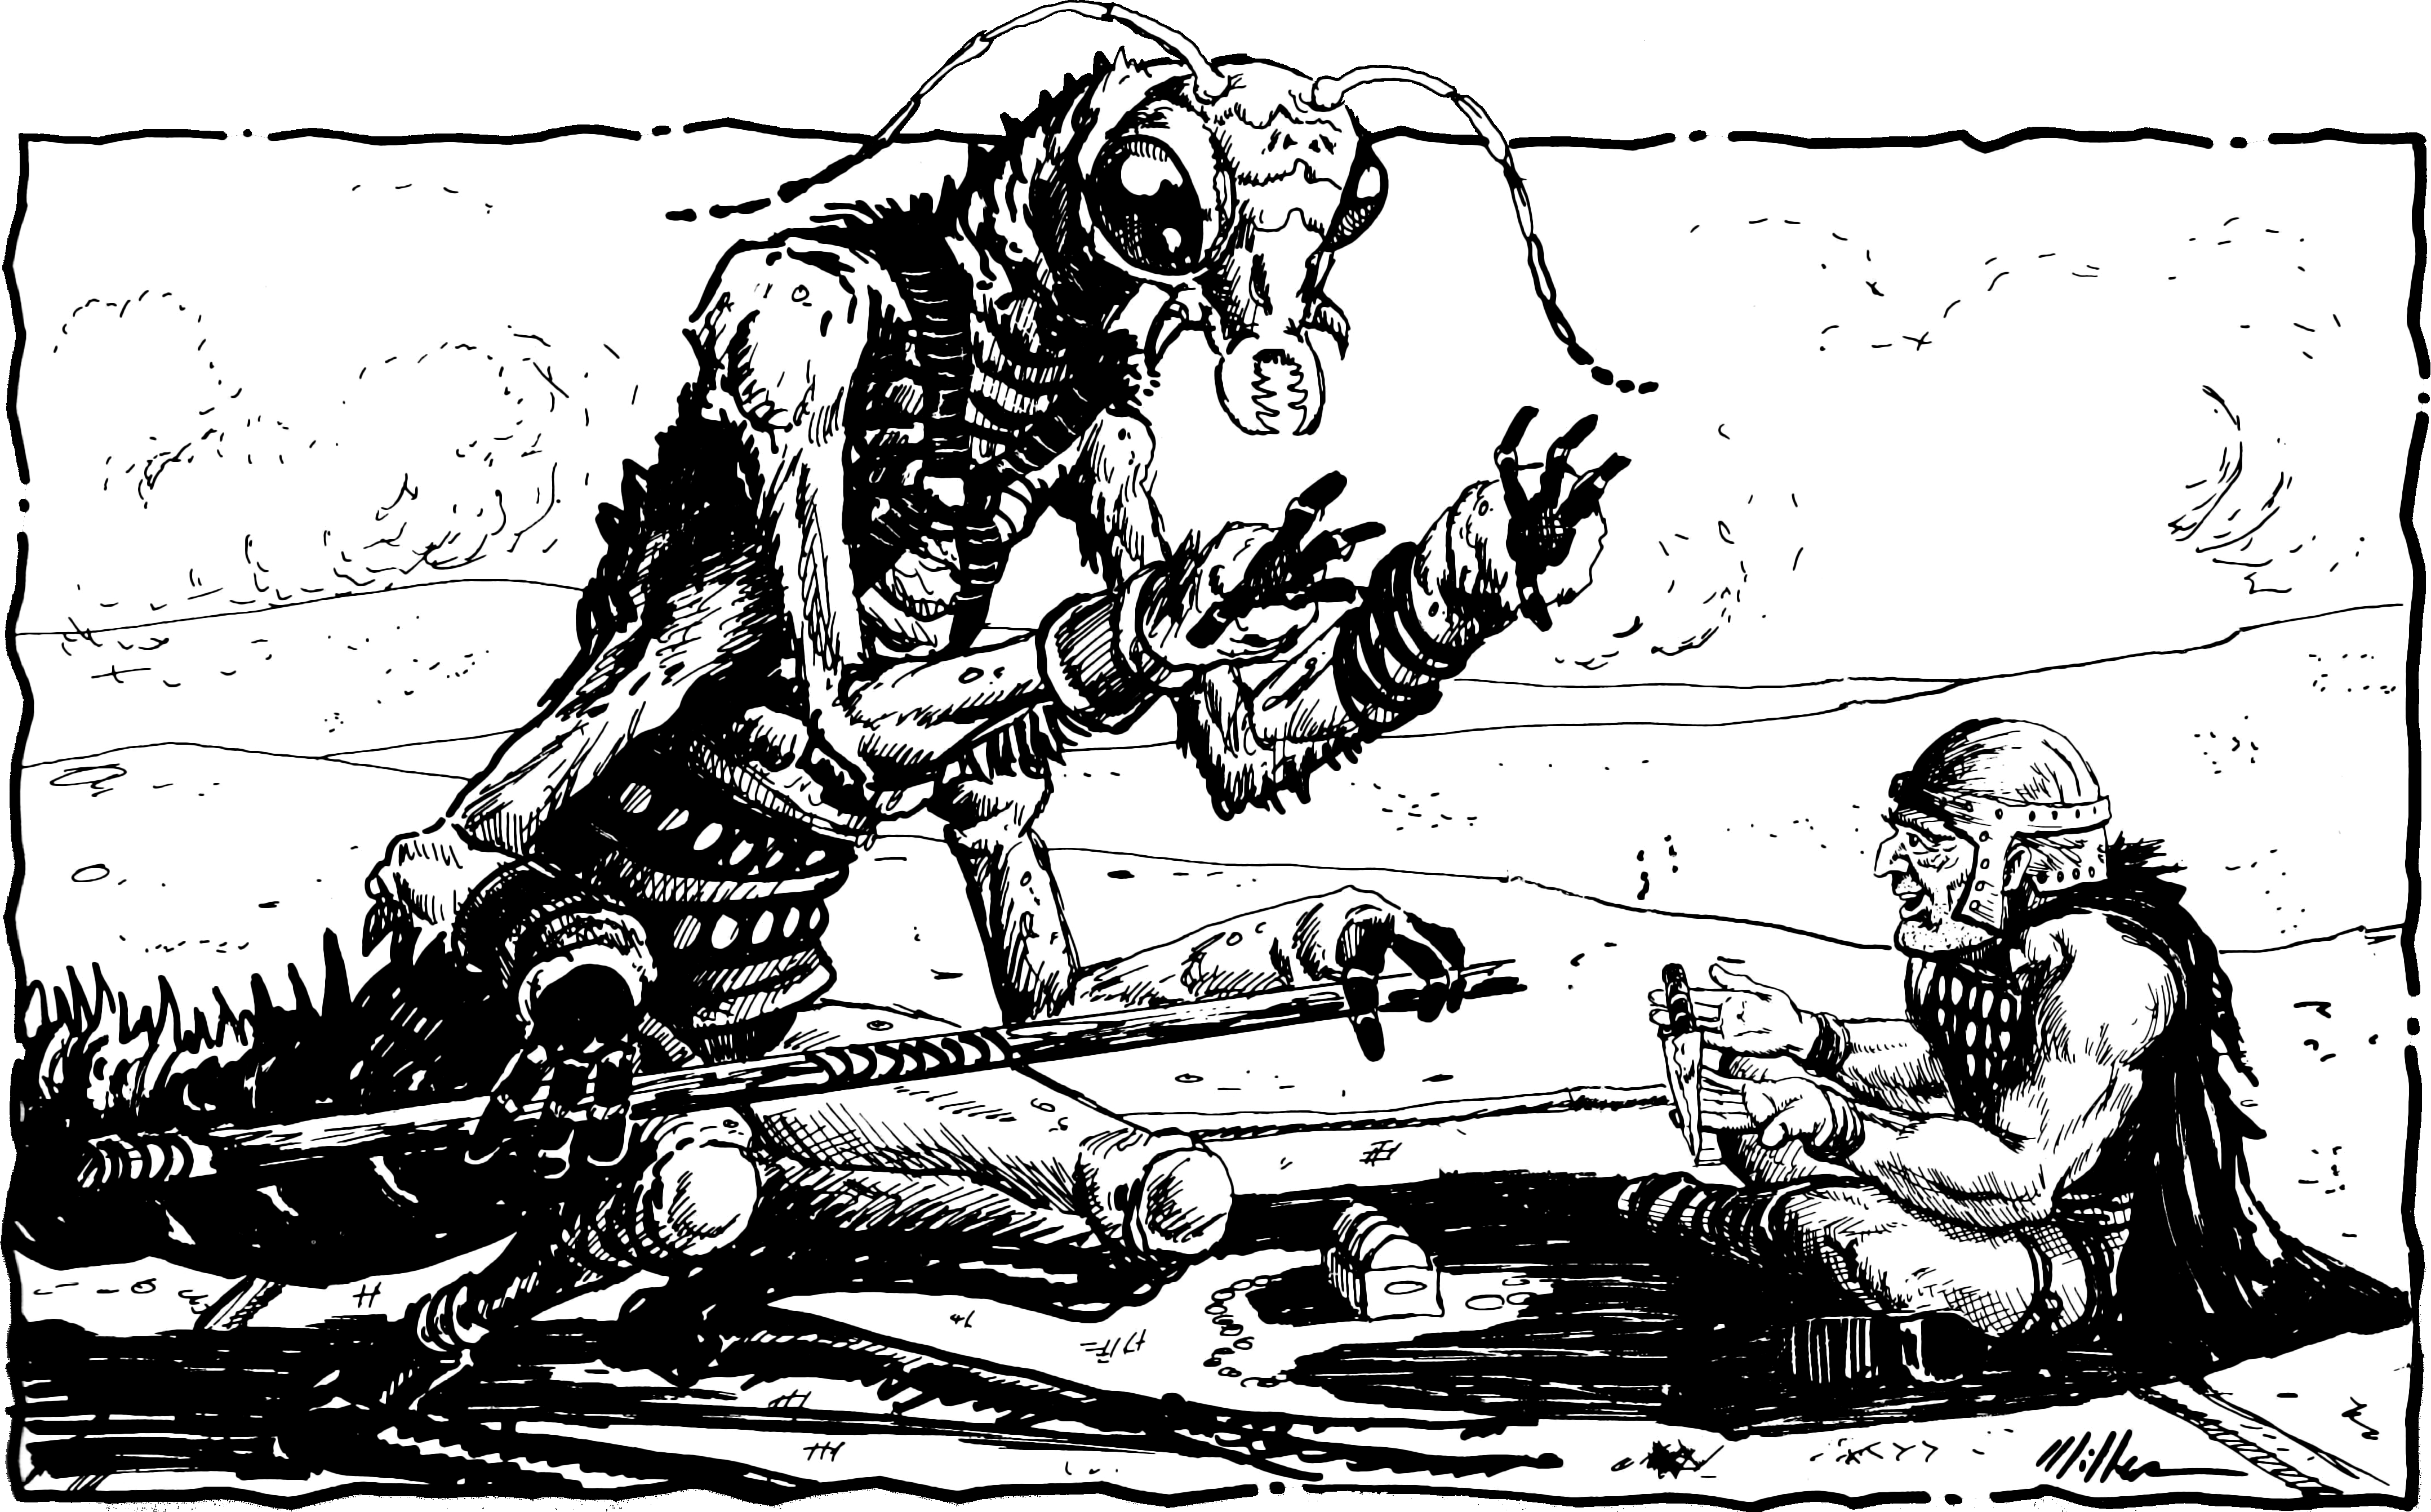
\includegraphics[width=\textwidth]{images/merchant-3.png}
\par\textit{\small\textcopyright Wizards of the Coast, 2020.}
\end{figure*}
\subsection{Documents}
This class of items has a symbolic function, conveying authority or permission. No price is listed for these items, because their value is not inherent.

\textbf{Letter of Marque}: This letter bears the personal mark of the sorcerer‐king, and bestows limited secular authority on the bearer, as if the bearer were a templar. The bearer of a letter of marque gains the authority to contest the actions of templars, using the bearer’s \skill{Diplomacy} check. If the bearer is already a templar, then having the letter as additional authority grants the templar a +4 circumstance check towards authority contest checks. The letter of marque does not grant the authority to Intrude, Requisition, Accuse or Judge, but does grant power to contest such actions by templars. A letter of marque is limited by time. After a specified period (usually one year, and never longer than seven years) the letter loses its effectiveness. A sorcerer‐king can also declare the letter invalid. Forging or fraudulently using a letter of marque is an unpardonable offense that brings a death sentence. Obviously, only the templars and other servants of the sorcerer‐king that issued the letter of marque will honor its terms. A person who is caught with a king’s letter of marque within another sorcerer‐king’s territory will have some explaining to do.

\textbf{Letter of Reprisal}: Like a letter of marque, this letter bears the personal mark of the sorcerer‐king, and bestows limited secular authority on the bearer, as if the bearer were a templar. Unlike a letter of marque, a letter of reprisal has a limited scope to carrying out a specific mission, usually a reprisal or retaliation against a specific group of the King’s enemies, for example, killing or capturing a specific enemy officer, capturing a particular enemy fortress or silt vessel, defiling a stretch of key farmland, or annihilating or enslaving a designated village. Depending on the bearer’s \skill{Diplomacy} ranks, she can Requisition, Intrude, Accuse, Judge, but only if she can show that her request relates to fulfilling her assigned mission. She can attempt to contest the actions of other templars, but takes a $-4$ circumstance penalty on such attempts, since the opposing templars can argue (even if it is not true) that she is acting outside of the scope of the assigned reprisal mission. The $-4$ penalty also applies if templars contest any of her Requisition, Intrude, Accuse, or Judge actions.
\subsectionA{Food, Drink, and Lodging}
Many Athasian travelers are lodged by merchant houses, elemental temples, psionic academies, or family. Adventurers, however, pay for hospitality.

\Table{Food, Drink, and Lodging}{XRR}{
\tableheader Item & \tableheader Cost & \tableheader Weight\\
\TableSubheader{Broy} &&\\
~ Keg (4 liters) & 2 cp & 5 kg\\
~ Mug & 4 bits & \onehalf kg\\
\TableSubheader{Inn stay (per day)} &&\\
~ Good & 2 sp & \\
~ Common & 5 cp & \\
~ Poor & 2 cp & \\
\TableSubheader{Meals (per day)} &&\\
~ Good & 5 bits & \\
~ Common & 3 bits & \\
~ Poor & 1 bit & \\
\TableSubheader{Water} &&\\
~ Keg (4 liters) & 2 bits & 5 kg\\
~ Mug & 1 bd & \onehalf kg\\
}

\textbf{Broy:} Broy is made from fermented kank nectar. Spiced broy and watered-down broy are also available. When served plain, it is potent and foul tasting. However, broy can be served warm and spiced with a pungent herb that disguises its sourness, as well as enhancing its enrapturing powers.

\textbf{Inn:} Poor accommodations at an inn amount to a place on the floor near the hearth. Common accommodations consist of a place on a raised, heated floor, the use of a blanket and a pillow. Good accommodations consist of a small, private room with one bed, some amenities, and a covered chamber pot in the corner.

\textbf{Meals:} Poor meals might be composed of bread, baked turnips, onions, and water. Common meals might consist of bread, chicken stew, carrots, and watered-down ale or wine. Good meals might be composed of bread and pastries, beef, peas, and ale or wine.
\subsectionA{Mounts and Related Gear}

\Table{Mounts and Related Gear}{XRR}{
\tableheader Goods or Services & \tableheader Cost & \tableheader Weight \\
\TableSubheader{Barding} &&\\
~ Medium creature & $\times$2 & $\times$1 \\
~ Large creature & $\times$4 & $\times$2 \\
Bit and bridle & 2 cp & \onehalf kg \\
Feed (per day) & 1 bit & 5 kg \\
\TableSubheader{Mounts} &&\\
~ \TableSubheader{Birds} &&\\
~ Erdland & 25 cp &\\
~ Erdlu & 10 cp &\\
~ \TableSubheader{Reptiles} &&\\
~ Crodlu, riding & 200 cp & \\
~ Crodlu, warmount & 400 cp & \\
~ Inix & 100 cp & \\
~ Mekillot & 200 cp & \\
~ \TableSubheader{Insects} &&\\
~ Kank, herding & 50 cp &\\
~ Kank, riding & 125 cp &\\
~ Kank, warmount & 250 cp &\\
\TableSubheader{Saddle} &&\\
~ Military & 20 cp & 15 kg \\
~ Pack & 5 cp & 7.5 kg \\
~ Riding & 10 cp & 12.5 kg \\
\TableSubheader{Saddle, Exotic} &&\\
~ Military & 60 cp & 20 kg \\
~ Pack & 15 cp & 10 kg \\
~ Riding & 30 cp & 15 kg \\
Saddlebags & 4 cp & 4 kg \\
Stabling (per day) & 5 bits &\\
}

\textbf{Barding, Medium Creature and Large Creature:} Barding is a type of armor that covers the head, neck, chest, body, and possibly legs of a horse or other mount. Barding made of medium or heavy armor provides better protection than light barding, but at the expense of speed. Barding can be made of any of the armor types found on \tabref{Armor and Shields}.

Armor for a horse (a Large nonhumanoid creature) costs four times as much as armor for a human (a Medium humanoid creature) and also weighs twice as much as the armor found on \tabref{Armor and Shields} (see Armor for Unusual Creatures). If the barding is for a pony or other Medium mount, the cost is only double, and the weight is the same as for Medium armor worn by a humanoid. Medium or heavy barding slows a mount that wears it, as shown on the table below.

Flying mounts can't fly in medium or heavy barding.

Removing and fitting barding takes five times as long as the figures given on \tabref{Donning Armor}. A barded animal cannot be used to carry any load other than the rider and normal saddlebags.

\Table{Barding}{XCCC}{
 & \multicolumn{3}{c}{\tableheader Base Speed}\\
\cmidrule[0.5pt]{2-4}
\tableheader Barding & \tableheader (12 m) & \tableheader (15 m) & \tableheader (18 m)\\
Medium & 9 m & 10.5 m & 12 m\\
Heavy & 9 m\footnotemark[1] & 10.5 m\footnotemark[1] & 12 m\footnotemark[1]\\

\TableNote{4}{1 A mount wearing heavy armor moves at only triple its normal speed when running instead of quadruple.}\\
}

\textbf{Crodlu:} A crodlu is a large bipedal lizard mount, resembling a scaled ostrich. A crodlu is appropriate as a mount for a Medium humanoid creature. Crodlu are hard to control in battle, while war crodlu can be ridden into battle easily. Crodlu benefit from stabling, can wear barding, and require feed like normal mounts.

\textbf{Erdland:} These creatures are large, flightless birds used as mounts or to pull caravans. They weigh around 2 tons and can stand up to 4.5 meters tall. An erdland is appropriate as a mount for a Medium humanoid creature. Erdlands can be ridden into battle easily. Erdlands benefit from stabling, can wear barding, and require feed like normal mounts.

\textbf{Erdlu:} Erdlus are a smaller variety of erdland, mostly used as herd beasts. They stand 2.1 meters tall and weigh around 100 kg. An erdlu is appropriate as a mount for a Medium humanoid creature. Erdlus are hard to control in battle. Erdlus benefit from stabling, can wear barding, and require feed like normal mounts.

\textbf{Feed:} Crodlus, erdlands, erdlus, inixes require feeding. Mekillots require eight times more than normal mounts.

\textbf{Inix:} The inix is a large, 5.5-meter long reptile commonly used for riding and as a beast of burden. An inix is appropriate as a mount for a Medium or Large humanoid creature. Inixes can be ridden into battle easily. Inixes benefit from stabling, can wear custom barding (specially constructed, adding an additional 50\% to the price), and require feed like normal mounts.

\textbf{Kank:} A kank is a large, 2.4-meter long insect, commonly used as a personal mount. These insects cannot be used as food, for their meat smells atrocious, but they produce highly nutritious globules of honey. A kank is appropriate as a mount for a Medium humanoid creature. Kanks are hard to control in battle. Kanks benefit from stabling, cannot wear barding, and do not require feeding.

\textbf{Mekillot:} A mekillot is a huge, 3,000-kg. lizard, used for hauling large cargo or serving as transportation for troops. These beasts are hard to control in combat and usually require a psionic handler. Mekillots benefit from stabling, can wear barding, and require feed eight times more than a normal mount.

\textbf{Saddle, Exotic:} An exotic saddle is like a normal saddle of the same sort except that it is designed for an unusual mount. Exotic saddles come in military, pack, and riding styles.

\textbf{Saddle, Military:} A military saddle braces the rider, providing advantage on \skill{Ride} checks related to staying in the saddle. If you're knocked unconscious while in a military saddle, you have a 75\% chance to stay in the saddle (compared to 50\% for a riding saddle).

\textbf{Saddle, Pack:} A pack saddle holds gear and supplies, but not a rider. It holds as much gear as the mount can carry.

\textbf{Saddle, Riding:} The standard riding saddle supports a rider.

\clearpage
\begin{figure}[t!]
\centering
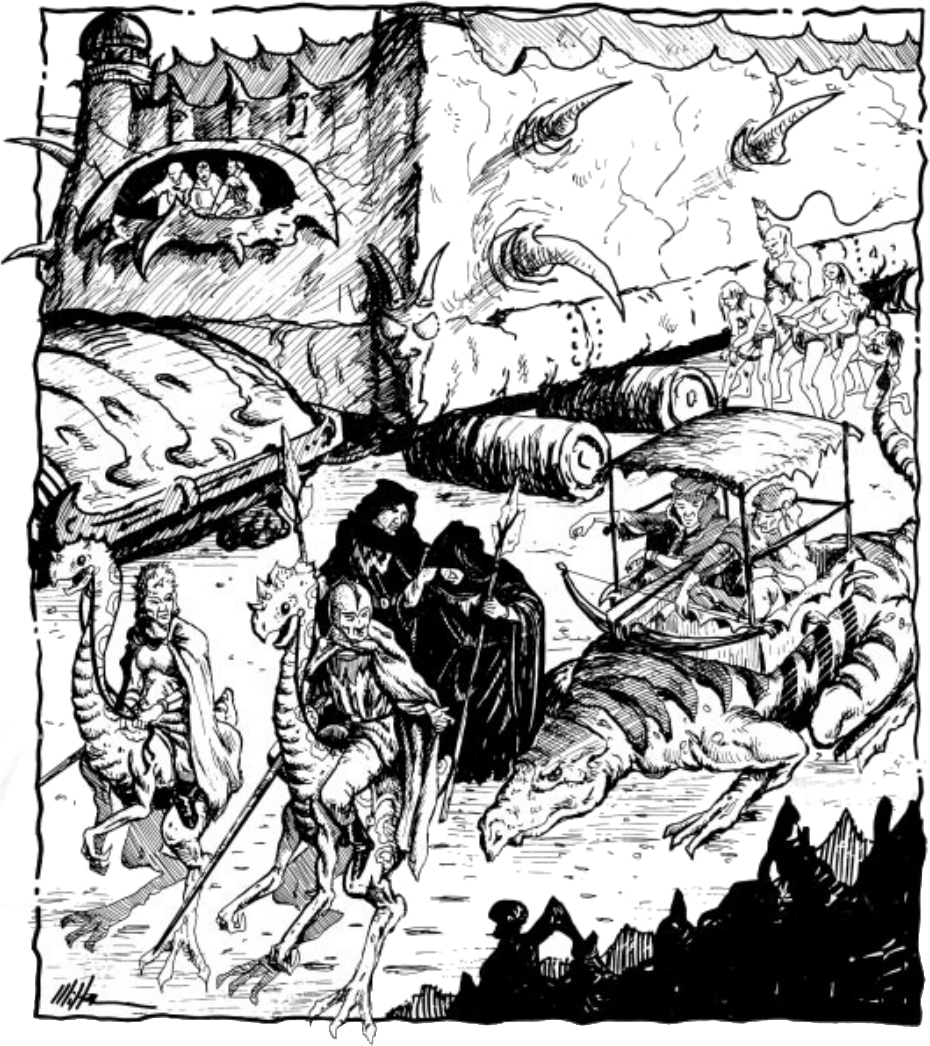
\includegraphics[width=\columnwidth]{images/caravan-3.png}
\par\textit{\small\textcopyright Wizards of the Coast, 2020.}
\end{figure}
\subsection{Transport}
Sometimes it is too hard or too dangerous to ride a kank---you'll need some other form of transportation. Some vehicles, such as the chariot and howdah, are moved by muscle power. The \skill{Handle Animal} skill is used only if that power comes from a team of draft animals. When the team consists of creatures with Intelligence scores of 3 or higher, the operative skill is \skill{Diplomacy}. When they are slaves or forced labor, the operative skill is \skill{Intimidate}.

\Table{Transport}{Xr{2cm}}{
\tableheader Transport & \tableheader Cost\\
Chariot, two-person, transport & 50 cp \\
Chariot, two-person, war & 125 cp \\
Chariot, four-person, war & 250 cp \\
Howdah, inix & 10 cp \\
Howdah, inix, war & 100 cp \\
Howdah, mekillot & 20 cp \\
Howdah, mekillot, war & 500 cp \\
Wagon, open, 500 kg capacity & 20 cp \\
Wagon, open, 1,250 kg capacity & 35 cp \\
Wagon, open, 2,500 kg capacity & 50 cp \\
Wagon, open, 5,000 kg capacity & 100 cp \\
Wagon, enclosed, 500 kg capacity & 40 cp \\
Wagon, enclosed, 1,250 kg capacity & 70 cp \\
Wagon, enclosed, 2,500 kg capacity & 100 cp \\
Wagon, enclosed, 5,000 kg capacity & 200 cp \\
Wagon, armored caravan & 1,000 cp \\
}

\textbf{Chariot}: A chariot is a two‐wheeled vehicle used for transportation, racing, war and processions. Transport chariots are very small and simple, requiring only a single animal to draw it. A war chariot built for two riders is slightly larger, but significantly better constructed. Generally one person will drive the chariot while the other uses a bow or other ranged weapon. A war chariot built for four is much larger than the other two kinds of chariots and requires at least two mounts to drive it. A war chariot offers cover to its occupants.

\textbf{Howdah}: A howdah is an enclosure mounted on a riding animal containing space for one or more persons. Howdahs can be fitted on inix or mekillots, and provide shade and cover from the elements. An inix howdah usually has room for only one person, though the war howdah, built much stronger, can hold four. A mekillot howdah can hold one or two persons, but a war howdah is much bigger, consisting of two levels and holding up to sixteen warriors.

\textbf{Wagon}: Wagons are an essential part of Athasian economy, as they facilitate the caravans that make life in the wastes possible. Open wagons are basic, open–topped wagons that can carry a certain amount of cargo. As Athasian wagons are built using little or no metal, there’s a limit to how much cargo they can carry. Open wagons generally require two beasts to draw them, but sometimes a single erdland will work.

\textit{Enclosed wagons}: They are more commonly used to transport people or fragile cargo that would otherwise be damaged by exposure to the elements.

\textit{Armored wagons}: They are primarily used by caravans traveling through areas plagued by dangerous monsters or raiders. It is an enclosed wagon with agafari wood used to strengthen the wagon throughout. There are also mount points for fixed crossbows on each side of that wagon that can swivel 180 degrees. Anyone using the crossbows or firing out of the rear of the wagon (when it is open) receives cover. Armored wagons require at least four smaller mounts to draw it, two inixes or one mekillot.

\subsectionA{Services}

\Table{Services}{lR}{
\tableheader Services & \tableheader Cost\\
Messenger         & 1 bit/km\\
Road or gate toll & 1 bit\\

\multicolumn{2}{l}{\TableSubheader{Hirelings, Military}}\\
Archer              & 1 bit/day  \\
Cavalry, heavy      & 3 bits/day \\
Cavalry, light      & 1 bit/day  \\
Crossbowman         & 5 bd/day   \\
Engineer            & 5 cp/day   \\
Infantry, heavy     & 5 bd/day   \\
Infantry, light     & 2 bd/day   \\
Infantry, irregular & 1 bd/day   \\

\multicolumn{2}{l}{\TableSubheader{Hirelings, Civilian}}\\
Draqoman                        & Level in cp/day \\
Craftsman\footnotemark[1]       & 1 bit/day      \\
Professional\footnotemark[2]    & 5 bd/day       \\
Specialist\footnotemark[3]      & 3 bits/day     \\
Spellcaster                     & 5 bits/day     \\
Unskilled labor\footnotemark[4] & 2 bd/day       \\


\multicolumn{2}{l}{\TableSubheader{Manifesting}}\\
Power, 1st--level & Manifester level $\times$ 10 cp\footnotemark[5]\\
Power, 2nd--level & Manifester level $\times$ 20 cp\footnotemark[5]\\
Power, 3rd--level & Manifester level $\times$ 30 cp\footnotemark[5]\\
Power, 4th--level & Manifester level $\times$ 40 cp\footnotemark[5]\\
Power, 5th--level & Manifester level $\times$ 50 cp\footnotemark[5]\\
Power, 6th--level & Manifester level $\times$ 60 cp\footnotemark[5]\\
Power, 7th--level & Manifester level $\times$ 70 cp\footnotemark[5]\\
Power, 8th--level & Manifester level $\times$ 80 cp\footnotemark[5]\\
Power, 9th--level & Manifester level $\times$ 90 cp\footnotemark[5]\\

\multicolumn{2}{l}{\TableSubheader{Spellcasting}}\\
Spell,   0--level & Caster level $\times$  5 sp\footnotemark[5]\footnotemark[6]\\
Spell, 1st--level & Caster level $\times$ 10 sp\footnotemark[5]\footnotemark[6]\\
Spell, 2nd--level & Caster level $\times$ 20 sp\footnotemark[5]\footnotemark[6]\\
Spell, 3rd--level & Caster level $\times$ 30 sp\footnotemark[5]\footnotemark[6]\\
Spell, 4th--level & Caster level $\times$ 40 sp\footnotemark[5]\footnotemark[6]\\
Spell, 5th--level & Caster level $\times$ 50 sp\footnotemark[5]\footnotemark[6]\\
Spell, 6th--level & Caster level $\times$ 60 sp\footnotemark[5]\footnotemark[6]\\
Spell, 7th--level & Caster level $\times$ 70 sp\footnotemark[5]\footnotemark[6]\\
Spell, 8th--level & Caster level $\times$ 80 sp\footnotemark[5]\footnotemark[6]\\
Spell, 9th--level & Caster level $\times$ 90 sp\footnotemark[5]\footnotemark[6]\\

\TableNote{2}{1 Any \skill{Craft} skill available.}\\
\TableNote{2}{2 Any \skill{Profession} skill available.}\\
\TableNote{2}{3 Any skill, other than Craft and Profession.}\\
\TableNote{2}{4 Jobs that do not require associated skills.}\\
\TableNote{2}{5 See its description for additional costs. If the additional costs put the total cost above 3,000 cp, that service is not generally available.}\\
\TableNote{2}{6 Spellcasting is considered high treason and spellcasters are not comfortable offering their services.}\\
}

Sometimes the best solution for a problem is to hire someone else to take care of it. Spellcasting, unless divine, is rarely, if ever, for sale on Athas. However, the manifesting of psionic powers for cash is much more common.

\textbf{Archer:} A 2nd-level fighter specialized in longbows, weilding a composite longbow (Str +2), and wearing studded leather and a buckler.

\textbf{Cavalry, Heavy:} A 2nd-level fighter wearing scale mail, and wielding a lance two-handed. They mount a heavy crodlu wearing a scale mail, as well.

\textbf{Cavalry, Light:} A 1st-level fighter wearing a studded leather and a wooden shield, and wielding a lance. They mount a light crodlu with no armor.

\textbf{Craftsman:} Usually a 2nd-level settler, but they can be of any class. This pays for any \skill{Craft} check of DC 20 or lower. Higher DC checks double the price for each 5 points of difference. 

\textbf{Crossbowman:} A 1st-level fighter specialized in crossbows, weilding a composite heavy crossbow (Str +4), and wearing studded scale mail and a tower shield.

\textbf{Draqoman:} A bard of 6th or higher level with at least one contact (see Alternative Class Features). Their wages depends on the bard's level and are the default price for skill contacts. If the draqoman has different types of contact, then they might double the price.

\textbf{Engineer:} A 5th-level fighter with 8 ranks of \skill{Knowledge} (warcraft) and a martial prowess that depend on this skill. They are equipped with \emph{breastplate +1} and a \emph{tower shield +1}. Although a military engineer has combat capabilities, their function is to oversee construction of siege engines and of static defenses.

\textbf{Infantry, Heavy:} A 2nd-level fighter, wearing a half-plate and tower shield, wielding a one-handed weapon. 

\textbf{Infantry, Light:} A 1st-level fighter, specialized either in spear and shields, or longswords. Light infantry usually wears studded leather, but caravan's infantry wear caravan armor.

\textbf{Infantry, Irregular:} A 2nd-level barbarian or gladiator. Their specialization is atypical, and they typically use gladiator armor or shell armor.

\textbf{Messenger:} This entry includes mounted messengers and runners. Those willing to carry a message to a place they were going anyway may ask for only half the indicated amount.

\textbf{Power:} The indicated amount is how much it costs to get a manifester to manifest a power for you. This cost assumes that you can go to the manifester and have the power manifested at his or her convenience. If you want to bring the manifester somewhere to manifest a power you need to negotiate with the manifester, otherwise the default answer is no.

The cost given is for a power with no XP cost. If the power has an XP cost, add 5 cp per XP lost.

Furthermore, if a power has dangerous consequences, the manifester will certainly require proof that you can and will pay for dealing with any such consequences (that is, assuming that the manifester even agrees to manifest such a power, which isn't certain). In the case of powers that transport the manifester and characters over a distance, you will likely have to pay for two manifestations of the power, even if you aren't returning with the manifester.

In addition, not every town or village has a manifester of sufficient level to manifest any power. In general, you must travel to a small town (or larger settlement) to be reasonably assured of finding a manifester capable of manifesting 1st--level powers, a large town for 2nd--level powers, a small city for 3rd-- or 4th--level powers, a large city for 5th-- or 6th--level powers, and a metropolis for 7th-- or 8th--level powers. Even a metropolis isn't guaranteed to have a local manifester able to cast 9th--level powers.

\textbf{Professional:} Usually a 2nd-level settler, but they can be of any class. This pays for any \skill{Profession} check of DC 20 or lower. Higher DC checks double the price for each 5 points of difference.

\textbf{Road or Gate Toll:} A toll is sometimes charged to cross a well-trodden, well-kept, and well-guarded road to pay for patrols on it and for its upkeep. Occasionally, a large walled city charges a toll to enter or exit (or sometimes just to enter).

\textbf{Specialist:} A 2nd-level NPC with \feat{Skill Focus} on the corresponding skill speciality, who can deliver a skill check of DC 20. Scouts are usually hired for \skill{Knowledge} (geography), \skill{Spot}, or \skill{Survival}. Thieves for \skill{Disable Device}, \skill{Forgery}, \skill{Open Lock}, \skill{Search}, or \skill{Sleight of Hand}. Bards for \skill{Appraise}, \skill{Diplomacy}, or \skill{Perform}. Wizards for \skill{Decipher Script}, any \skill{Knowledge}, or \skill{Spellcraft}. These are guidelines, but the wages are the same for any class.

\textbf{Spell:} The indicated amount is how much it costs to get a spellcaster to cast a spell for you. This cost assumes that you can go to the spellcaster and have the spell cast at his or her convenience (generally at least 24 hours later, so that the spellcaster has time to prepare the spell in question). If you want to bring the spellcaster somewhere to cast a spell you need to negotiate with him or her, and the default answer is no.

The cost given is for a spell with no cost for a material component or focus component and no XP cost. If the spell includes a material component, add the cost of that component to the cost of the spell.

If the spell has a focus component (other than a divine focus), add 1/10 the cost of that focus to the cost of the spell. If the spell has an XP cost, add 5 cp per XP lost.

Furthermore, if a spell has dangerous consequences, the spellcaster will certainly require proof that you can and will pay for dealing with any such consequences (that is, assuming that the spellcaster even agrees to cast such a spell, which isn't certain). In the case of spells that transport the caster and characters over a distance, you will likely have to pay for two castings of the spell, even if you aren't returning with the caster.

In addition, not every town or village has a spellcaster of sufficient level to cast any spell. In general, you must travel to a small town (or larger settlement) to be reasonably assured of finding a spellcaster capable of casting 1st--level spells, a large town for 2nd--level spells, a small city for 3rd-- or 4th--level spells, a large city for 5th-- or 6th--level spells, and a metropolis for 7th-- or 8th--level spells. Even a metropolis isn't guaranteed to have a local spellcaster able to cast 9th--level spells.

\textbf{Spellcaster:} A 3rd-level cleric or wizard. These wages do not pay for expensive material components, which must be given by the employer.

\textbf{Unskilled Labor:} Any job that a freeman might do that does not require a skill check.


\section{Special Materials}
A number of exotic materials can be found in the wilds and underground of the Tablelands and beyond, in addition to the more mundane ones. These substances have innate special properties. If you make a suit of armor or weapon out of more than one special material, you get the benefit of only the most prevalent material. However, you can build a double weapon with each head made of a different special material.

\subsection{Special Weapons Materials}
Each of the special materials described below has a definite game effect. Some creatures have damage reduction based on their creature type or core concept. Some are resistant to all but a special type of damage, such as that dealt by evil-aligned weapons or bludgeoning weapons. Others are vulnerable to weapons of a particular material. Characters may choose to carry several different types of weapons, depending upon the campaign and types of creatures they most commonly encounter.

\Table{Special Materials Cost Modifiers}{Xr{2.6cm}}{
\tableheader Type of Item & \tableheader Item Cost Modifier\\
\TableSubheader{Adamantine (dwarven steel)} &\\
Ammunition & +60 gp\\
Weapon & +3,000 gp\\
Shield & +2,000 gp\\
Light armor & +5,000 gp\\
Medium armor & +10,000 gp\\
Heavy armor & +15,000 gp\\

\TableSubheader{Agafari} &\\
Any wooden item & $\star$ + 20 cp per kg\\

\TableSubheader{Crystal, deep} &\\
Any weapon & +1,000 cp\\

\TableSubheader{Crystal, living} &\\
Ammunition & +250 cp\\
Light weapon & +750 gp\\
One-handed weapon, or one head of a double weapon & +1,000 gp\\
Two-handed weapon, or both heads of a double weapon & +1,500 gp\\
Light armor & +2,000 cp\\
Medium armor & +5,000 cp\\
Heavy armor & +9,000 cp\\

\TableSubheader{Crystal, mundane} &\\
Any armor, shield, or weapon & $\star$\\

\TableSubheader{Dasl} &\\
Any weapon & $\times$10\\

\TableSubheader{Drakehide} &\\
Any armor or shield & $\star$ $\times$ 2\\

\TableSubheader{Drake Ivory} &\\
Any weapon & $\times$2\\

\TableSubheader{Iron} &\\
Any armor, shield, or weapon & $\times$100\\

\TableSubheader{Silver, alchemical} &\\
Ammunition & +2 gp\\
Light weapon & +20 gp\\
One-handed weapon, or one head of a double weapon & +90 gp\\
Two-handed weapon, or both heads of a double weapon & +180 gp\\

\TableNote{2}{$\star$ Masterwork price}
}

\textbf{Adamantine}: While weapons and armor made from adamantine, also called ``dwarven steel'', can be found on Athas, they are quite rare. Nearly all items made from adamantine are relics from a long past age, scavenged from ruins by elves and treasure hunters. Raw adamantine cannot be bought on the market, and weapons and armor constructed from adamantine are considered priceless relics.

This ultrahard metal adds to the quality of a weapon or suit of armor. Weapons fashioned from adamantine have a natural ability to bypass hardness when sundering weapons or attacking objects, ignoring hardness less than 20. Armor made from adamantine grants its wearer damage reduction of 1/-- if it's light armor, 2/-- if it's medium armor, and 3/-- if it's heavy armor. Adamantine is so costly that weapons and armor made from it are always of masterwork quality; the masterwork cost is included in the prices. Thus, adamantine weapons and ammunition have a +1 enhancement bonus on attack rolls, and the armor check penalty of adamantine armor is lessened by 1 compared to ordinary armor of its type. Items without metal parts cannot be made from adamantine. An arrow could be made of adamantine, but a quarterstaff could not.

Only weapons, armor, and shields normally made of metal can be fashioned from adamantine. Weapons, armor and shields normally made of steel that are made of adamantine have one-third more hit points than normal. Adamantine has 40 hit points per inch of thickness and hardness 20.

\textbf{Agafari}: This rare magic wood is as hard as normal wood but very light. Any wooden or mostly wooden item (such as a bow, an arrow, or a spear) made from agadari is considered a masterwork item and weighs only half as much as a normal wooden item of that type. Items not normally made of wood or only partially of wood (such as a battleaxe or a mace) either cannot be made from agadari or do not gain any special benefit from being made of agadari. The armor check penalty of a agadari shield is lessened by 2 compared to an ordinary shield of its type. To determine the price of a agadari item, use the original weight but add 20 cp per kilogram to the price of a masterwork version of that item.

For weapons affected by the inferior material rule, agafari is considered an inferior material.

Agafari has 10 hit points per inch of thickness and hardness 5.

\textbf{Crystal, Deep}: Deep crystal is crystal of above-average quality found at the hearts of large veins or deposits of mundane crystal (see below). Deep crystal is renowned for its strength and its psionically resonant nature. Mundane crystal is used for many items of psionic manufacture, such as dorjes, power stones, and psicrystals. Deep crystal is a better grade.

While a weapon made of deep crystal is no different from a mundane crystal weapon for a nonpsionic character, a psionic wielder of a deep crystal weapon can focus psionic power through it, increasing the damage that weapon deals. As a free action that does not provoke attacks of opportunity, the wielder can channel psionic power into a melee weapon or ranged weapon made of deep crystal. For 2 power points, the deep crystal weapon deals an extra 2d6 points of damage. The weapon will stay charged for 1 minute or until it scores its next hit. Bows, crossbows, and slings bestow this power on their ammunition. All missile weapons lose this effect if they miss. However, they may be recovered and charged again.

Any weapon made of deep crystal costs 1,000 cp more than its noncrystal counterpart. Any item could potentially be made out of deep crystal. Because deep crystal armor is considered to be made out of metal, druids cannot wear it.

Deep crystal has 30 hit points per inch of thickness and hardness 10.

\textbf{Crystal, Living}: Living crystal is crystal of above-average quality renowned for its strength and its psionically-resonant nature. It is actually two different materials: the crystalline web material of a crystal spider used in making weapons, and the tissue of the crystal spider itself for making armor. The freshly-taken material must be treated within a day of its extraction by channeling psionic power into it, preserving its inherent psionic nature. One power point is required for every treated pound of material.

While a weapon made of living crystal is no different from a mundane crystal weapon (see below) for a nonpsionic character, a psionic wielder of a living crystal weapon can focus psionic power through it, increasing the damage that weapon deals. As a free action that does not provoke attacks of opportunity, and with the expediture of his psionic focus, the wielder can channel psionic power into a melee weapon or ranged weapon made of living crystal. For 2 power points, the living crystal weapon deals an extra 2d6 points of damage. The weapon will stay charged for 1 minute or until it scores its next hit. Bows, crossbows, and slings bestow this power on their ammunition. All missile weapons lose this effect if they miss. However, they may be recovered and charged again. For weapons affected by the inferior material rule, living crystal is considered inferior.

Armor made of living crystal is no different than metal armor for a nonpsionic character, but a psionic wearer of living crystal armor can focus psionic power through it, gaining an amount of damage reduction in the process. As a free action that does not provoke attacks of opportunity, and with the expediture of his psionic focus, the wearer can channel psionic power into armor made of living crystal. For 2 power points, the living crystal armor confers to the wearer damage reduction 5/metal. The armor will stay charged for 1 minute or until a hit is scored on it, whether or not the damage reduction applies to that particular hit. Unlike metal armor, living crystal armor isn't considered made of metal so druids can wear it without penalty.

Living crystal has 15 hit points per inch of thickness and hardness 8.

\textbf{Crystal, Mundane}: Mundane crystal can be used in place of metal in weapons or armor, using a special forging process. The fortified crystal possesses the properties of a similar masterwork steel weapon or armor, except for visual appearance.

Weapons and armor made of mundane crystal cost the same amount to make as their masterwork counterparts. Any item could potentially be made with mundane crystal. Because mundane crystal armor is considered to be made out of metal, druids cannot wear it.

Mundane crystal properly forged has 25 hit points per inch of thickness and a hardness of 8.

\textbf{Dasl}: Dasl is a special kind of crystalline material created by thri-kreen and often used to manufacture their weapons. An item made from dasl is treated as if it was made from iron and is not considered to be made from inferior materials. However, for purposes of harming creatures with damage reduction, a dasl weapon is not treated as being made from metal. An item made from dasl costs ten times what it normally would. Thus, a dasl chatkcha costs 200 cp instead of the 20 cp a stone or bone chatkcha would.

Dasl has a 15 hit points per inch of thickness and hardness 7.

\textbf{Drakehide}: The hide of a drake is of such value that most sorcerer-kings forbid their sale. They have instructed templars to confiscate any such items that appear in the market in the name of their sorcerer-king. Because drakes are so rare it is easy for templars to claim the item was stolen from the sorcerer-king and have the seller put to death. Elves, of course, defy these edicts at every turn, and make a fair profit selling drake materials while just one step ahead of their templar pursuers.

Armorsmiths can work with the hides of drakes to produce armor or shields of masterwork quality. One drake produces enough hide for four suits of hide armor, three suits of banded mail, two suits of half-plate, or one suit of full plate for a Medium creature. Enough hide is available to produce a small or large masterwork shield in addition to the armor.

Because dragonhide armor isn't made of metal, druids can wear it without penalty.

Drakehide armor costs double what masterwork armor of that type ordinarily costs, but it takes no longer to make than ordinary armor of that type.

Drakehide has 10 hit points per inch of thickness and hardness 10.

\textbf{Drake Ivory}: Drake ivory is extraordinarily strong and easy to work compared to the bone that most Athasian weaponsmiths use. Since it can only be obtained from the claws and teeth of deadly drakes, it is rare, expensive, and forbidden (see drakehide, above).

Weapons made from drake ivory cost an additional 2,000 cp to enchant. Weapons crafted from drake ivory cost twice what they normally would. A double weapon that is only half crafted using drake ivory increases its cost by 50\%.

Drake ivory has 30 hit points per inch of thickness and hardness 10.

% Giant Hair: Giant hair is very strong and frequently woven together to form a very strong cord. While sometimes used in armor, it is most frequently used to create rope. This rope costs 50 cp for 15 meters, has a hardness of 5 and 2 hp per inch of thickness

\textbf{Iron}: Iron (and most other metals) is rare on Athas, but weapons and armor made of iron can still be found. In all of the city-states, there are at least a few craftsmen that are able to work iron. The only fresh source of iron is the mines in the city-state of Tyr. Many of the iron weapons and armor available for sale have been scavenged from ruins. Weapons made of iron (including iron-based compounds like steel) can bypass the damage reduction possessed by some Athasian monsters. Iron-based items cost 100 times what they normally would.

Iron has 30 hit points per inch of thickness and hardness 10.

\textbf{Silver, Alchemical}: The process of binding silver to weapons has been greatly refined on Athas. Very little silver is actually needed in the process, and it can be bound to weapons crafted from dasl, obsidian and bone, as well as those made from iron.

A complex process involving metallurgy and alchemy can bond silver to a weapon made of steel so that it bypasses the damage reduction of creatures such as lycanthropes.

On a successful attack with a silvered weapon, the wielder takes a $-1$ penalty on the damage roll (with the usual minimum of 1 point of damage). The alchemical silvering process can't be applied to nonmetal items, and it doesn't work on rare metals such as adamantine, cold iron, and mithral.

Alchemical silver has 10 hit points per inch of thickness and hardness 8.

% magic items 10
% combat 11
% adventure 12
\Chapter{Magic}
{The Tablelands are a giant wasteland, to the untrained eye barren and devoid of life. When people see plants wither and die when someone utters mysterious phrases accompanied by unknown gestures, they assume the worst. They cry wizard and the mob instantly gathers to kill him. But if people venture into the wastes and look under the rocks, they will learn that Athas is teeming with all sorts of life. And when the vermin swarm forth to envelop them, biting and crawling into every orifice, do they see the irony?}
{The Oracle, Blue Shrine Scrolls}

\Capitalize{A}{} spell is a one-time magical effect. Spells come in two types: arcane (cast by wizards) and divine (cast by clerics, druids, experienced rangers, and templars). Some spellcasters select their spells from a limited list of spells known, while others have access to a wide variety of options.

Most spellcasters prepare their spells in advance---whether from a spellbook or through devout prayers and meditation---while some cast spells spontaneously without preparation.

Despite these different ways that characters use to learn or prepare their spells, when it comes to casting them, the spells are very much alike.

Cutting across the categories of arcane and divine spells are the eight schools of magic. These schools represent the different ways that spells take effect.

\Figure*{t}{images/magic-1.png}
\section{Casting Spells}
Whether a spell is arcane or divine, and whether a character prepares spells in advance or chooses them on the spot, casting a spell works the same way.

\subsection{Choosing A Spell}
First you must choose which spell to cast. If you're a cleric, druid, experienced ranger, or wizard, you select from among spells prepared earlier in the day and not yet cast (see Preparing Wizard Spells and Preparing Divine Spells).

If you're a templar, you can select any spell you know, provided you are capable of casting spells of that level or higher.

To cast a spell, you must be able to speak (if the spell has a verbal component), gesture (if it has a somatic component), and manipulate the material components or focus (if any). Additionally, you must concentrate to cast a spell.

If a spell has multiple versions, you choose which version to use when you cast it. You don't have to prepare a specific version of the spell.

Once you've cast a prepared spell, you can't cast it again until you prepare it again. (If you've prepared multiple copies of a single spell, you can cast each copy once.) If you're a templar, casting a spell counts against your daily limit for spells of that spell level, but you can cast the same spell again if you haven't reached your limit.

\subsection{Concentration}
To cast a spell, you must concentrate. If something interrupts your concentration while you're casting, you must make a \skill{Concentration} check or lose the spell. The more distracting the interruption and the higher the level of the spell you are trying to cast, the higher the DC is. If you fail the check, you lose the spell just as if you had cast it to no effect.

\textbf{Injury}: If while trying to cast a spell you take damage, you must make a \skill{Concentration} check (DC 10 + points of damage taken + the level of the spell you're casting). If you fail the check, you lose the spell without effect. The interrupting event strikes during spellcasting if it comes between when you start and when you complete a spell (for a spell with a casting time of 1 full round or more) or if it comes in response to your casting the spell (such as an attack of opportunity provoked by the spell or a contingent attack, such as a readied action).

If you are taking continuous damage half the damage is considered to take place while you are casting a spell. You must make a \skill{Concentration} check (DC 10 + \onehalf the damage that the continuous source last dealt + the level of the spell you're casting). If the last damage dealt was the last damage that the effect could deal then the damage is over, and it does not distract you.

Repeated damage does not count as continuous damage.

\textbf{Spell}: If you are affected by a spell while attempting to cast a spell of your own, you must make a \skill{Concentration} check or lose the spell you are casting. If the spell affecting you deals damage, the DC is 10 + points of damage + the level of the spell you're casting.

If the spell interferes with you or distracts you in some other way, the DC is the spell's saving throw DC + the level of the spell you're casting. For a spell with no saving throw, it's the DC that the spell's saving throw would have if a save were allowed.

\textbf{Grappling or Pinned}: The only spells you can cast while grappling or pinned are those without somatic components and whose material components (if any) you have in hand. Even so, you must make a \skill{Concentration} check (DC 20 + the level of the spell you're casting) or lose the spell.

\textbf{Vigorous Motion}: If you are riding on a moving mount, taking a bouncy ride in a wagon, on a small boat in rough water, below-decks in a storm-tossed ship, or simply being jostled in a similar fashion, you must make a \skill{Concentration} check (DC 10 + the level of the spell you're casting) or lose the spell.

\textbf{Violent Motion}: If you are on a galloping horse, taking a very rough ride in a wagon, on a small boat in rapids or in a storm, on deck in a storm-tossed ship, or being tossed roughly about in a similar fashion, you must make a \skill{Concentration} check (DC 15 + the level of the spell you're casting) or lose the spell.

\textbf{Violent Weather}: You must make a \skill{Concentration} check if you try to cast a spell in violent weather. If you are in a high wind carrying blinding rain or sleet, the DC is 5 + the level of the spell you're casting. If you are in wind-driven hail, dust, or debris, the DC is 10 + the level of the spell you're casting. In either case, you lose the spell if you fail the \skill{Concentration} check. If the weather is caused by a spell, use the rules in the Spell subsection above.

\textbf{Casting Defensively}: If you want to cast a spell without provoking any attacks of opportunity, you must make a \skill{Concentration} check (DC 15 + the level of the spell you're casting) to succeed. You lose the spell if you fail.

\textbf{Entangled}: If you want to cast a spell while entangled in a net or by a tanglefoot bag or while you're affected by a spell with similar effects, you must make a DC 15 \skill{Concentration} check to cast the spell. You lose the spell if you fail.
\subsection{Counterspells}
It is possible to cast any spell as a counterspell. By doing so, you are using the spell's energy to disrupt the casting of the same spell by another character. Counterspelling works even if one spell is divine and the other arcane.

\textbf{How Counterspells Work:} To use a counterspell, you must select an opponent as the target of the counterspell. You do this by choosing the ready action. In doing so, you elect to wait to complete your action until your opponent tries to cast a spell. (You may still move your speed, since ready is a standard action.)

If the target of your counterspell tries to cast a spell, make a \skill{Spellcraft} check (DC 15 + the spell's level). This check is a free action. If the check succeeds, you correctly identify the opponent's spell and can attempt to counter it. If the check fails, you can't do either of these things.

To complete the action, you must then cast the correct spell. As a general rule, a spell can only counter itself. If you are able to cast the same spell and you have it prepared (if you prepare spells), you cast it, altering it slightly to create a counterspell effect. If the target is within range, both spells automatically negate each other with no other results.

\textbf{Counterspelling Metamagic Spells:} Metamagic feats are not taken into account when determining whether a spell can be countered

\textbf{Specific Exceptions:} Some spells specifically counter each other, especially when they have diametrically opposed effects.

\textbf{Dispel Magic as a Counterspell:} You can use dispel magic to counterspell another spellcaster, and you don't need to identify the spell he or she is casting. However, dispel magic doesn't always work as a counterspell.

\subsection{Caster Level}
A spell's power often depends on its caster level, which for most spellcasting characters is equal to your class level in the class you're using to cast the spell.

You can cast a spell at a lower caster level than normal, but the caster level you choose must be high enough for you to cast the spell in question, and all level-dependent features must be based on the same caster level.

In the event that a class feature, domain granted power, or other special ability provides an adjustment to your caster level, that adjustment applies not only to effects based on caster level (such as range, duration, and damage dealt) but also to your caster level check to overcome your target's spell resistance and to the caster level used in dispel checks (both the dispel check and the DC of the check).

\textbf{Caster Level Checks:} To make a caster level check, roll 1d20 and add your caster level (in the relevant class). If the result equals or exceeds the DC (or the spell resistance, in the case of caster level checks made for spell resistance), the check succeeds.

\subsection{Spell Failure}
If you ever try to cast a spell in conditions where the characteristics of the spell cannot be made to conform, the casting fails and the spell is wasted.

Spells also fail if your concentration is broken and might fail if you're wearing armor while casting a spell with somatic components.

\subsection{The Spell's Result}
Once you know which creatures (or objects or areas) are affected, and whether those creatures have made successful saving throws (if any were allowed), you can apply whatever results a spell entails.

\Figure*{t}{images/magic-3.png}
\subsection{Special Spell Effects}
Many special spell effects are handled according to the school of the spells in question Certain other special spell features are found across spell schools.

\textbf{Attacks:} Some spell descriptions refer to attacking. All offensive combat actions, even those that don't damage opponents are considered attacks. Attempts to turn or rebuke undead count as attacks. All spells that opponents resist with saving throws, that deal damage, or that otherwise harm or hamper subjects are attacks. Spells that summon monsters or other allies are not attacks because the spells themselves don't harm anyone.

\textbf{Bonus Types:} Usually, a bonus has a type that indicates how the spell grants the bonus. The important aspect of bonus types is that two bonuses of the same type don't generally stack. With the exception of dodge bonuses, most circumstance bonuses, and racial bonuses, only the better bonus works (see Combining Magical Effects, below). The same principle applies to penalties---a character taking two or more penalties of the same type applies only the worst one.

\textbf{Bringing Back the Dead:} Several spells have the power to restore slain characters to life.

When a living creature dies, its soul departs its body, leaves the Material Plane, travels through the Astral Plane, and goes to abide on the plane where the creature's deity resides. If the creature did not worship a deity, its soul departs to the plane corresponding to its alignment. Bringing someone back from the dead means retrieving his or her soul and returning it to his or her body.

\textit{Level Loss:} Any creature brought back to life usually loses one level of experience. The character's new XP total is midway between the minimum needed for his or her new (reduced) level and the minimum needed for the next one. If the character was 1st level at the time of death, he or she loses 2 points of Constitution instead of losing a level.

This level loss or Constitution loss cannot be repaired by any mortal means, even \spell{wish} or \spell{miracle}. A revived character can regain a lost level by earning XP through further adventuring. A revived character who was 1st level at the time of death can regain lost points of Constitution by improving his or her Constitution score when he or she attains a level that allows an ability score increase.

\textit{Preventing Revivification:} Enemies can take steps to make it more difficult for a character to be returned from the dead. Keeping the body prevents others from using \spell{raise dead} or \spell{resurrection} to restore the slain character to life. Casting \spell{trap the soul} prevents any sort of revivification unless the soul is first released.

\textit{Revivification against One's Will:} A soul cannot be returned to life if it does not wish to be. A soul knows the name, alignment, and patron deity (if any) of the character attempting to revive it and may refuse to return on that basis.


\subsection{Combining Magical Effects}
Spells or magical effects usually work as described, no matter how many other spells or magical effects happen to be operating in the same area or on the same recipient. Except in special cases, a spell does not affect the way another spell operates. Whenever a spell has a specific effect on other spells, the spell description explains that effect. Several other general rules apply when spells or magical effects operate in the same place:

\textbf{Stacking Effects:} Spells that provide bonuses or penalties on attack rolls, damage rolls, saving throws, and other attributes usually do not stack with themselves. More generally, two bonuses of the same type don't stack even if they come from different spells (or from effects other than spells; see Bonus Types, above).

\textit{Different Bonus Names:} The bonuses or penalties from two different spells stack if the modifiers are of different types. A bonus that isn't named stacks with any bonus.

\textit{Same Effect More than Once in Different Strengths:} In cases when two or more identical spells are operating in the same area or on the same target, but at different strengths, only the best one applies.

\textit{Same Effect with Differing Results:} The same spell can sometimes produce varying effects if applied to the same recipient more than once. Usually the last spell in the series trumps the others. None of the previous spells are actually removed or dispelled, but their effects become irrelevant while the final spell in the series lasts.

\textit{One Effect Makes Another Irrelevant:} Sometimes, one spell can render a later spell irrelevant. Both spells are still active, but one has rendered the other useless in some fashion.

\textit{Multiple Mental Control Effects:} Sometimes magical effects that establish mental control render each other irrelevant, such as a spell that removes the subjects ability to act. Mental controls that don't remove the recipient's ability to act usually do not interfere with each other. If a creature is under the mental control of two or more creatures, it tends to obey each to the best of its ability, and to the extent of the control each effect allows. If the controlled creature receives conflicting orders simultaneously, the competing controllers must make opposed Charisma checks to determine which one the creature obeys.

\textbf{Spells with Opposite Effects:} Spells with opposite effects apply normally, with all bonuses, penalties, or changes accruing in the order that they apply. Some spells negate or counter each other. This is a special effect that is noted in a spell's description.

\textbf{Instantaneous Effects:} Two or more spells with instantaneous durations work cumulatively when they affect the same target.
\subsection{Sensory Effects}
The stealthy preserver crouches low behind the stone walls of the ruins, fumbling through his belt pouch for his material components, peering cautiously around for signs of the approaching gith marauders. Breathless, he draws out his precious may also have effects that appeal to the senses of components and begins his chant and hand motions. Verbal, somatic, and material components are all in play, but what's really happening? What are the sensory effects associated with casting a spell?

On Athas the casting of magical spells often draws unwanted attention. The sensory effects of casting and the ways a wizard might cover, expand, or mimic them are acutely important. These sensory effects relate directly to detection; the greater the effects during casting, the greater the chance the wizard is found out. Of course, when a wizard wishes to dramatically announce his spellcasting abilities, the greater the effects the better.

All spells have both a visual and aural effect during casting. Middle-level (4th- to 6th-level) spells may also have effects that appeal to the senses of touch and smell. High-level spells may have grand effects.

Sensory effects for casting are particular to each spellcaster. The effects themselves remain constant for each sensory category, no matter what the spell level.

\textbf{Visual effects:} Streaks of sparkling multicolored light emerge from the vanishing material components, follow the movements of the spell's somatics (if any), then settle on the subject of the spell. The sparkling lights slightly illuminate the caster and target of the spell for the spell's entire casting time. Brightness is determined by spell level; color varies by spell and by caster. Other possible effects include glowing rings of light, heatless flames, and so on. A visual effect cannot substitute for an existing spell such as \spell{light} or the various illusions.

\textbf{Aural effects:} Along with any verbal components, a shimmer like that of tiny, metal wind chimes accompanies the caster's words, rising and falling with the spell's somatics. The jingling emanates from the caster's location, rising from silence to its maximum volume and back to silence over the casting time. Volume is determined by spell level. Other possible effects include a roaring wind, thousands of slithering snakes, etc.

\textbf{Olfactory effects:} For spells with olfactory sensory effects, an odor unique to the caster or the spell permeates the air. The smell may be pleasant, such as flowers or perfumes, or quite unpleasant, such as rotting meat. Intensity of the smell is determined by spell level.

\textbf{Tactile effects:} Creatures near the caster feel something brush up against them. The nature of the sensation can be soft and pleasant, such as feathers, or abrasive, such as grit or jagged bone. Intensity of the sensation is determined by spell level.

\textbf{Grand effects:} Spells of especially high level may cause grand effects in casting. The ground may tremble, rocking tables and tipping over bottles. The weather may temporarily change, clouding over ominously, wind picking up or stopping, temperature growing abnormally hot or chill.

\Table{Sensory Effects of Casting}{lCCC}{
\tableheader Spell Level & \tableheader Visual/Aural & \tableheader Olfactory/Tacticle & \tableheader Grand \\
1st--3rd & Yes & No       & No       \\
4th--6th & Yes & Optional & No       \\
7th--9th & Yes & Yes      & Optional \\
}


\subsubsection{Detecting Spellcasting}
Whenever a spell is cast, there is a chance that any casual observer will notice it. Aural and visual effects require \skill{Listen} and \skill{Spot} checks, respectively. Olfactory and tacticle effects require Wisdom checks, and the DC increases by 1 for each 3 meters of distance between the spellcaster and the observer. Grand effects are automatically detected. DC for each check is 10 minus the spell level.

% \Table{Sensory Range}{lCCC}{
% \tableheader Spell Level & \tableheader Visual/Aural & \tableheader Olfactory/Tacticle & \tableheader Grand \\
% 1st--3rd & 18 m &      &      \\
% 4th--6th & 27 m & 18 m &      \\
% 7th--9th & 36 m & 27 m & 36 m \\	
% }


\section{Spell Descriptions}
The description of each spell is presented in a standard format. Each category of information is explained and defined below.


\subsection{Name}
The first line of every spell description gives the name by which the spell is generally known.

\subsection{School (Subschool)}
Beneath the spell name is a line giving the school of magic (and the subschool, if appropriate) that the spell belongs to.

Almost every spell belongs to one of eight schools of magic. A school of magic is a group of related spells that work in similar ways. A small number of spells (arcane mark, limited wish, permanency, prestidigitation, and wish) are universal, belonging to no school.

\textbf{Abjuration}: Abjurations are protective spells. They create physical or magical barriers, negate magical or physical abilities, harm trespassers, or even banish the subject of the spell to another plane of existence.

If one abjuration spell is active within 10 feet of another for 24 hours or more, the magical fields interfere with each other and create barely visible energy fluctuations. The DC to find such spells with the Search skill drops by 4.

If an abjuration creates a barrier that keeps certain types of creatures at bay, that barrier cannot be used to push away those creatures. If you force the barrier against such a creature, you feel a discernible pressure against the barrier. If you continue to apply pressure, you end the spell.

\textbf{Conjuration}: Each conjuration spell belongs to one of five subschools. Conjurations bring manifestations of objects, creatures, or some form of energy to you (the summoning subschool), actually transport creatures from another plane of existence to your plane (calling), heal (healing), transport creatures or objects over great distances (teleportation), or create objects or effects on the spot (creation). Creatures you conjure usually, but not always, obey your commands.

A creature or object brought into being or transported to your location by a conjuration spell cannot appear inside another creature or object, nor can it appear floating in an empty space. It must arrive in an open location on a surface capable of supporting it.

The creature or object must appear within the spell's range, but it does not have to remain within the range.

\textit{Calling}: A calling spell transports a creature from another plane to the plane you are on. The spell grants the creature the one-time ability to return to its plane of origin, although the spell may limit the circumstances under which this is possible. Creatures who are called actually die when they are killed; they do not disappear and reform, as do those brought by a summoning spell (see below). The duration of a calling spell is instantaneous, which means that the called creature can't be dispelled.

\textit{Creation}: A creation spell manipulates matter to create an object or creature in the place the spellcaster designates (subject to the limits noted above). If the spell has a duration other than instantaneous, magic holds the creation together, and when the spell ends, the conjured creature or object vanishes without a trace. If the spell has an instantaneous duration, the created object or creature is merely assembled through magic. It lasts indefinitely and does not depend on magic for its existence.

\textit{Healing}: Certain divine conjurations heal creatures or even bring them back to life.

\textit{Summoning}: A summoning spell instantly brings a creature or object to a place you designate. When the spell ends or is dispelled, a summoned creature is instantly sent back to where it came from, but a summoned object is not sent back unless the spell description specifically indicates this. A summoned creature also goes away if it is killed or if its hit points drop to 0 or lower. It is not really dead. It takes 24 hours for the creature to reform, during which time it can't be summoned again.

When the spell that summoned a creature ends and the creature disappears, all the spells it has cast expire. A summoned creature cannot use any innate summoning abilities it may have, and it refuses to cast any spells that would cost it XP, or to use any spell-like abilities that would cost XP if they were spells.

\textit{Teleportation}: A teleportation spell transports one or more creatures or objects a great distance. The most powerful of these spells can cross planar boundaries. Unlike summoning spells, the transportation is (unless otherwise noted) one-way and not dispellable.

Teleportation is instantaneous travel through the Astral Plane. Anything that blocks astral travel also blocks teleportation.

\textbf{Divination}: Divination spells enable you to learn secrets long forgotten, to predict the future, to find hidden things, and to foil deceptive spells.

Many divination spells have cone-shaped areas. These move with you and extend in the direction you look. The cone defines the area that you can sweep each round. If you study the same area for multiple rounds, you can often gain additional information, as noted in the descriptive text for the spell.

\textit{Scrying}: A scrying spell creates an invisible magical sensor that sends you information. Unless noted otherwise, the sensor has the same powers of sensory acuity that you possess. This level of acuity includes any spells or effects that target you, but not spells or effects that emanate from you. However, the sensor is treated as a separate, independent sensory organ of yours, and thus it functions normally even if you have been blinded, deafened, or otherwise suffered sensory impairment.

Any creature with an Intelligence score of 12 or higher can notice the sensor by making a DC 20 Intelligence check. The sensor can be dispelled as if it were an active spell.

Lead sheeting or magical protection blocks a scrying spell, and you sense that the spell is so blocked.

\textbf{Enchantment}: Enchantment spells affect the minds of others, influencing or controlling their behavior.

All enchantments are mind-affecting spells. Two types of enchantment spells grant you influence over a subject creature.

\textit{Charm}: A charm spell changes how the subject views you, typically making it see you as a good friend.

\textit{Compulsion}: A compulsion spell forces the subject to act in some manner or changes the way her mind works. Some compulsion spells determine the subject's actions or the effects on the subject, some compulsion spells allow you to determine the subject's actions when you cast the spell, and others give you ongoing control over the subject.

\textbf{Evocation}: Evocation spells manipulate energy or tap an unseen source of power to produce a desired end. In effect, they create something out of nothing. Many of these spells produce spectacular effects, and evocation spells can deal large amounts of damage.

\textbf{Illusion}: Illusion spells deceive the senses or minds of others. They cause people to see things that are not there, not see things that are there, hear phantom noises, or remember things that never happened.

\textit{Figment}: A figment spell creates a false sensation. Those who perceive the figment perceive the same thing, not their own slightly different versions of the figment. (It is not a personalized mental impression.) Figments cannot make something seem to be something else. A figment that includes audible effects cannot duplicate intelligible speech unless the spell description specifically says it can. If intelligible speech is possible, it must be in a language you can speak. If you try to duplicate a language you cannot speak, the image produces gibberish. Likewise, you cannot make a visual copy of something unless you know what it looks like.

Because figments and glamers (see below) are unreal, they cannot produce real effects the way that other types of illusions can. They cannot cause damage to objects or creatures, support weight, provide nutrition, or provide protection from the elements. Consequently, these spells are useful for confounding or delaying foes, but useless for attacking them directly.

A figment's AC is equal to 10 + its size modifier.

\textit{Glamer}: A glamer spell changes a subject's sensory qualities, making it look, feel, taste, smell, or sound like something else, or even seem to disappear.

\textit{Pattern}: Like a figment, a pattern spell creates an image that others can see, but a pattern also affects the minds of those who see it or are caught in it. All patterns are mind-affecting spells.

\textit{Phantasm}: A phantasm spell creates a mental image that usually only the caster and the subject (or subjects) of the spell can perceive. This impression is totally in the minds of the subjects. It is a personalized mental impression. (It's all in their heads and not a fake picture or something that they actually see.) Third parties viewing or studying the scene don't notice the phantasm. All phantasms are mind-affecting spells.

\textit{Shadow}: A shadow spell creates something that is partially real from extradimensional energy. Such illusions can have real effects. Damage dealt by a shadow illusion is real.

\textit{Saving Throws and Illusions (Disbelief)}: Creatures encountering an illusion usually do not receive saving throws to recognize it as illusory until they study it carefully or interact with it in some fashion.

A successful saving throw against an illusion reveals it to be false, but a figment or phantasm remains as a translucent outline.

A failed saving throw indicates that a character fails to notice something is amiss. A character faced with proof that an illusion isn't real needs no saving throw. If any viewer successfully disbelieves an illusion and communicates this fact to others, each such viewer gains a saving throw with a +4 bonus.

\textbf{Necromancy}: Necromancy spells manipulate the power of death, unlife, and the life force. Spells involving undead creatures make up a large part of this school.

\textbf{Transmutation}: Transmutation spells change the properties of some creature, thing, or condition.


\subsection{[Descriptor]}
Appearing on the same line as the school and subschool, when applicable, is a descriptor that further categorizes the spell in some way. Some spells have more than one descriptor.

The descriptors are acid, air, chaotic, cold, darkness, death, earth, electricity, evil, fear, fire, force, good, language-dependent, lawful, light, mind-affecting, ritual, sonic, and water.

Most of these descriptors have no game effect by themselves, but they govern how the spell interacts with other spells, with special abilities, with unusual creatures, with alignment, and so on.

A language-dependent spell uses intelligible language as a medium for communication. If the target cannot understand or cannot hear what the caster of a language-dependent spell says the spell fails.

A mind-affecting spell works only against creatures with an Intelligence score of 1 or higher.

A ritual spell can be cast following the normal rules for spellcasting, or the spell can be cast as a ritual.


\subsection{Level}
The next line of a spell description gives the spell's level, a number between 0 and 9 that defines the spell's relative power. This number is preceded by an abbreviation for the class whose members can cast the spell. The Level entry also indicates whether a spell is a domain spell and, if so, what its domain and its level as a domain spell are. A spell's level affects the DC for any save allowed against the effect.

Names of spellcasting classes are abbreviated as follows: cleric Clr; druid Drd; ranger Rgr; templar Tmp; wizard Wiz.

The domains a spell can be associated with include Agriculture, Air, Animal, Chaos, Charm, Cleansing, Cycle, Death, Decay, Destruction, Drought, Earth, Fire, Forecasting, Freedom, Glory, Growth, Knowledge, Law, Madness, Magic, Magma, Mind, Mirage, Nobility, Plant, Protection, Purity, Rain, Replenishment, Silt, Strength, Sun, Travel, Trickery, War, Water, and Wrath.

\Figure{b}{images/wizard-7.png}
\Figure*{t}{images/magic-2.png}
\subsection{Components}
A spell's components are what you must do or possess to cast it. The Components entry in a spell description includes abbreviations that tell you what type of components it has. Specifics for material, focus, and XP components are given at the end of the descriptive text. Usually you don't worry about components, but when you can't use a component for some reason or when a material or focus component is expensive, then the components are important.

\textbf{Verbal (V)}: A verbal component is a spoken incantation. To provide a verbal component, you must be able to speak in a strong voice. A silence spell or a gag spoils the incantation (and thus the spell). A spellcaster who has been deafened has a 20\% chance to spoil any spell with a verbal component that he or she tries to cast.

\textbf{Somatic (S)}: A somatic component is a measured and precise movement of the hand. You must have at least one hand free to provide a somatic component.

\textbf{Material (M)}: A material component is one or more physical substances or objects that are annihilated by the spell energies in the casting process. Unless a cost is given for a material component, the cost is negligible. Don't bother to keep track of material components with negligible cost. Assume you have all you need as long as you have your spell component pouch.

\textbf{Focus (F)}: A focus component is a prop of some sort. Unlike a material component, a focus is not consumed when the spell is cast and can be reused. As with material components, the cost for a focus is negligible unless a price is given. Assume that focus components of negligible cost are in your spell component pouch.

\textbf{Divine Focus (DF)}: A divine focus component is an item of spiritual significance. The divine focus for a cleric or a paladin is a holy symbol appropriate to the character's faith.

If the Components line includes F/DF or M/DF, the arcane version of the spell has a focus component or a material component (the abbreviation before the slash) and the divine version has a divine focus component (the abbreviation after the slash).

\textbf{XP Cost (XP)}: Some powerful spells entail an experience point cost to you. No spell can restore the XP lost in this manner. You cannot spend so much XP that you lose a level, so you cannot cast the spell unless you have enough XP to spare. However, you may, on gaining enough XP to attain a new level, use those XP for casting a spell rather than keeping them and advancing a level. The XP are treated just like a material component---expended when you cast the spell, whether or not the casting succeeds.
\subsection{Casting Time}
Most spells have a casting time of 1 standard action. Others take 1 round or more, while a few require only a free action.

A spell that takes 1 round to cast is a full-round action. It comes into effect just before the beginning of your turn in the round after you began casting the spell. You then act normally after the spell is completed.

A spell that takes 1 minute to cast comes into effect just before your turn 1 minute later (and for each of those 10 rounds, you are casting a spell as a full-round action, just as noted above for 1-round casting times). These actions must be consecutive and uninterrupted, or the spell automatically fails.

When you begin a spell that takes 1 round or longer to cast, you must continue the concentration from the current round to just before your turn in the next round (at least). If you lose concentration before the casting is complete, you lose the spell.

A spell with a casting time of 1 free action doesn't count against your normal limit of one spell per round. However, you may cast such a spell only once per round. Casting a spell with a casting time of 1 free action doesn't provoke attacks of opportunity.

You make all pertinent decisions about a spell (range, target, area, effect, version, and so forth) when the spell comes into effect.

\subsection{Range}
A spell's range indicates how far from you it can reach, as defined in the Range entry of the spell description. A spell's range is the maximum distance from you that the spell's effect can occur, as well as the maximum distance at which you can designate the spell's point of origin. If any portion of the spell's area would extend beyond this range, that area is wasted. Standard ranges include the following.

\textbf{Personal:} The spell affects only you.

\textbf{Touch:} You must touch a creature or object to affect it. A touch spell that deals damage can score a critical hit just as a weapon can. A touch spell threatens a critical hit on a natural roll of 20 and deals double damage on a successful critical hit. Some touch spells allow you to touch multiple targets. You can touch as many willing targets as you can reach as part of the casting, but all targets of the spell must be touched in the same round that you finish casting the spell.

\textbf{Close:} The spell reaches as far as 7.5 meters away from you. The maximum range increases by 1.5 meter for every two full caster levels.

\textbf{Medium:} The spell reaches as far as 30 meters + 3 meters per caster level.

\textbf{Long:} The spell reaches as far as 120 meters + 12 meters per caster level.

\textbf{Unlimited:} The spell reaches anywhere on the same plane of existence.

\textbf{Range Expressed in Meters:} Some spells have no standard range category, just a range expressed in meters.
\subsection{Aiming A Spell}
You must make some choice about whom the spell is to affect or where the effect is to originate, depending on the type of spell. The next entry in a spell description defines the spell's target (or targets), its effect, or its area, as appropriate.

\textbf{Target or Targets}: Some spells have a target or targets. You cast these spells on creatures or objects, as defined by the spell itself. You must be able to see or touch the target, and you must specifically choose that target. You do not have to select your target until you finish casting the spell.

If the target of a spell is yourself (the spell description has a line that reads Target: You), you do not receive a saving throw, and spell resistance does not apply. The Saving Throw and Spell Resistance lines are omitted from such spells.

Some spells restrict you to willing targets only. Declaring yourself as a willing target is something that can be done at any time (even if you're flat-footed or it isn't your turn). Unconscious creatures are automatically considered willing, but a character who is conscious but immobile or helpless (such as one who is bound, cowering, grappling, paralyzed, pinned, or stunned) is not automatically willing.

Some spells allow you to redirect the effect to new targets or areas after you cast the spell. Redirecting a spell is a move action that does not provoke attacks of opportunity.

\textbf{Effect}: Some spells create or summon things rather than affecting things that are already present.

You must designate the location where these things are to appear, either by seeing it or defining it. Range determines how far away an effect can appear, but if the effect is mobile it can move regardless of the spell's range.

\textit{Ray}: Some effects are rays. You aim a ray as if using a ranged weapon, though typically you make a ranged touch attack rather than a normal ranged attack. As with a ranged weapon, you can fire into the dark or at an invisible creature and hope you hit something. You don't have to see the creature you're trying to hit, as you do with a targeted spell. Intervening creatures and obstacles, however, can block your line of sight or provide cover for the creature you're aiming at.

If a ray spell has a duration, it's the duration of the effect that the ray causes, not the length of time the ray itself persists.

If a ray spell deals damage, you can score a critical hit just as if it were a weapon. A ray spell threatens a critical hit on a natural roll of 20 and deals double damage on a successful critical hit.

\textit{Spread}: Some effects, notably clouds and fogs, spread out from a point of origin, which must be a grid intersection. The effect can extend around corners and into areas that you can't see. Figure distance by actual distance traveled, taking into account turns the spell effect takes. When determining distance for spread effects, count around walls, not through them. As with movement, do not trace diagonals across corners. You must designate the point of origin for such an effect, but you need not have line of effect (see below) to all portions of the effect.

\textbf{Area}: Some spells affect an area. Sometimes a spell description specifies a specially defined area, but usually an area falls into one of the categories defined below.

Regardless of the shape of the area, you select the point where the spell originates, but otherwise you don't control which creatures or objects the spell affects. The point of origin of a spell is always a grid intersection. When determining whether a given creature is within the area of a spell, count out the distance from the point of origin in squares just as you do when moving a character or when determining the range for a ranged attack. The only difference is that instead of counting from the center of one square to the center of the next, you count from intersection to intersection.

You can count diagonally across a square, but remember that every second diagonal counts as 2 squares of distance. If the far edge of a square is within the spell's area, anything within that square is within the spell's area. If the spell's area only touches the near edge of a square, however, anything within that square is unaffected by the spell.

\textit{Burst, Emanation, or Spread}: Most spells that affect an area function as a burst, an emanation, or a spread. In each case, you select the spell's point of origin and measure its effect from that point.

A burst spell affects whatever it catches in its area, even including creatures that you can't see. It can't affect creatures with total cover from its point of origin (in other words, its effects don't extend around corners). The default shape for a burst effect is a sphere, but some burst spells are specifically described as cone-shaped. A burst's area defines how far from the point of origin the spell's effect extends.

An emanation spell functions like a burst spell, except that the effect continues to radiate from the point of origin for the duration of the spell. Most emanations are cones or spheres.

A spread spell spreads out like a burst but can turn corners. You select the point of origin, and the spell spreads out a given distance in all directions. Figure the area the spell effect fills by taking into account any turns the spell effect takes.

\textit{Cone, Cylinder, Line, or Sphere}: Most spells that affect an area have a particular shape, such as a cone, cylinder, line, or sphere.

A cone-shaped spell shoots away from you in a quarter-circle in the direction you designate. It starts from any corner of your square and widens out as it goes. Most cones are either bursts or emanations (see above), and thus won't go around corners.

When casting a cylinder-shaped spell, you select the spell's point of origin. This point is the center of a horizontal circle, and the spell shoots down from the circle, filling a cylinder. A cylinder-shaped spell ignores any obstructions within its area.

A line-shaped spell shoots away from you in a line in the direction you designate. It starts from any corner of your square and extends to the limit of its range or until it strikes a barrier that blocks line of effect. A line-shaped spell affects all creatures in squares that the line passes through.

A sphere-shaped spell expands from its point of origin to fill a spherical area. Spheres may be bursts, emanations, or spreads.

\textit{Creatures}: A spell with this kind of area affects creatures directly (like a targeted spell), but it affects all creatures in an area of some kind rather than individual creatures you select. The area might be a spherical burst, a cone-shaped burst, or some other shape.

Many spells affect ``living creatures,'' which means all creatures other than constructs and undead. Creatures in the spell's area that are not of the appropriate type do not count against the creatures affected.

\textit{Objects}: A spell with this kind of area affects objects within an area you select (as Creatures, but affecting objects instead).

\textit{Other}: A spell can have a unique area, as defined in its description.

\textit{(S) Shapeable}: If an Area or Effect entry ends with ``(S),'' you can shape the spell. A shaped effect or area can have no dimension smaller than 10 feet. Many effects or areas are given as cubes to make it easy to model irregular shapes. Three-dimensional volumes are most often needed to define aerial or underwater effects and areas.

\textbf{Line of Effect}: A line of effect is a straight, unblocked path that indicates what a spell can affect. A line of effect is canceled by a solid barrier. It's like line of sight for ranged weapons, except that it's not blocked by fog, darkness, and other factors that limit normal sight.

You must have a clear line of effect to any target that you cast a spell on or to any space in which you wish to create an effect. You must have a clear line of effect to the point of origin of any spell you cast.

A burst, cone, cylinder, or emanation spell affects only an area, creatures, or objects to which it has line of effect from its origin (a spherical burst's center point, a cone-shaped burst's starting point, a cylinder's circle, or an emanation's point of origin).

An otherwise solid barrier with a hole of at least 1 square foot through it does not block a spell's line of effect. Such an opening means that the 5-foot length of wall containing the hole is no longer considered a barrier for purposes of a spell's line of effect.
\subsection{Duration}
A spell's Duration entry tells you how long the magical energy of the spell lasts.

\textbf{Timed Durations:} Many durations are measured in rounds, minutes, hours, or some other increment. When the time is up, the magic goes away and the spell ends. If a spell's duration is variable the duration is rolled secretly (the caster doesn't know how long the spell will last).

\textbf{Instantaneous:} The spell energy comes and goes the instant the spell is cast, though the consequences might be long-lasting.

\textbf{Permanent:} The energy remains as long as the effect does. This means the spell is vulnerable to dispel magic.

\textbf{Concentration:} The spell lasts as long as you concentrate on it. Concentrating to maintain a spell is a standard action that does not provoke attacks of opportunity. Anything that could break your concentration when casting a spell can also break your concentration while you're maintaining one, causing the spell to end.

You can't cast a spell while concentrating on another one. Sometimes a spell lasts for a short time after you cease concentrating.

\textbf{Subjects, Effects, and Areas:} If the spell affects creatures directly the result travels with the subjects for the spell's duration. If the spell creates an effect, the effect lasts for the duration. The effect might move or remain still. Such an effect can be destroyed prior to when its duration ends. If the spell affects an area then the spell stays with that area for its duration.

Creatures become subject to the spell when they enter the area and are no longer subject to it when they leave.

\textbf{Touch Spells and Holding the Charge:} In most cases, if you don't discharge a touch spell on the round you cast it, you can hold the charge (postpone the discharge of the spell) indefinitely. You can make touch attacks round after round. If you cast another spell, the touch spell dissipates.

Some touch spells allow you to touch multiple targets as part of the spell. You can't hold the charge of such a spell; you must touch all targets of the spell in the same round that you finish casting the spell.

\textbf{Discharge:} Occasionally a spells lasts for a set duration or until triggered or discharged.

\textbf{(D) Dismissible:} If the Duration line ends with  ``(D),'' you can dismiss the spell at will. You must be within range of the spell's effect and must speak words of dismissal, which are usually a modified form of the spell's verbal component. If the spell has no verbal component, you can dismiss the effect with a gesture. Dismissing a spell is a standard action that does not provoke attacks of opportunity.

A spell that depends on concentration is dismissible by its very nature, and dismissing it does not take an action, since all you have to do to end the spell is to stop concentrating on your turn.
\subsection{Saving Throw}
Usually a harmful spell allows a target to make a saving throw to avoid some or all of the effect. The Saving Throw entry in a spell description defines which type of saving throw the spell allows and describes how saving throws against the spell work.

\textbf{Negates}: The spell has no effect on a subject that makes a successful saving throw.

\textbf{Partial}: The spell causes an effect on its subject. A successful saving throw means that some lesser effect occurs.

\textbf{Half}: The spell deals damage, and a successful saving throw halves the damage taken (round down).

\textbf{None}: No saving throw is allowed.

\textbf{Disbelief}: A successful save lets the subject ignore the effect.

\textbf{(object)}: The spell can be cast on objects, which receive saving throws only if they are magical or if they are attended (held, worn, grasped, or the like) by a creature resisting the spell, in which case the object uses the creature's saving throw bonus unless its own bonus is greater. (This notation does not mean that a spell can be cast only on objects. Some spells of this sort can be cast on creatures or objects.) A magic item's saving throw bonuses are each equal to 2 + one-half the item's caster level.

\textbf{(harmless)}: The spell is usually beneficial, not harmful, but a targeted creature can attempt a saving throw if it desires.

\textbf{Saving Throw Difficulty Class}: A saving throw against your spell has a DC of 10 + the level of the spell + your bonus for the relevant ability (Intelligence for a wizard, Charisma for a templar, or Wisdom for a cleric, druid, and ranger). A spell's level can vary depending on your class. Always use the spell level applicable to your class.

\textbf{Succeeding on a Saving Throw}: A creature that successfully saves against a spell that has no obvious physical effects feels a hostile force or a tingle, but cannot deduce the exact nature of the attack. Likewise, if a creature's saving throw succeeds against a targeted spell you sense that the spell has failed. You do not sense when creatures succeed on saves against effect and area spells.

\textbf{Automatic Failures and Successes}: A natural 1 (the d20 comes up 1) on a saving throw is always a failure, and the spell may cause damage to exposed items (see Items Surviving after a Saving Throw, below). A natural 20 (the d20 comes up 20) is always a success.

\textbf{Voluntarily Giving up a Saving Throw}: A creature can voluntarily forego a saving throw and willingly accept a spell's result. Even a character with a special resistance to magic can suppress this quality.

\textbf{Items Surviving after a Saving Throw}: Unless the descriptive text for the spell specifies otherwise, all items carried or worn by a creature are assumed to survive a magical attack. If a creature rolls a natural 1 on its saving throw against the effect, however, an exposed item is harmed (if the attack can harm objects). Refer to \tabref{Items Affected by Magical Attacks}. Determine which four objects carried or worn by the creature are most likely to be affected and roll randomly among them. The randomly determined item must make a saving throw against the attack form and take whatever damage the attack deal.

If an item is not carried or worn and is not magical, it does not get a saving throw. It simply is dealt the appropriate damage.

\Table{Items Affected by Magical Attacks}{lX}{
\tableheader Order\footnotemark[1] & \tableheader Item\\
1st & Shield\\
2nd & Armor\\
3rd & Magic helmet, hat, or headband\\
4th & Item in hand (including weapon, wand, or the like)\\
5th & Magic cloak\\
6th & Stowed or sheathed weapon\\
7th & Magic bracers\\
8th & Magic clothing\\
9th & Magic jewelry (including rings)\\
10th & Anything else\\

\TableNote{2}{1 In order of most likely to least likely to be affected.}\\
}


\subsection{Spell Resistance}
Spell resistance is a special defensive ability. If your spell is being resisted by a creature with spell resistance, you must make a caster level check (1d20 + caster level) at least equal to the creature's spell resistance for the spell to affect that creature. The defender's spell resistance is like an Armor Class against magical attacks. Include any adjustments to your caster level to this caster level check.

The Spell Resistance entry and the descriptive text of a spell description tell you whether spell resistance protects creatures from the spell. In many cases, spell resistance applies only when a resistant creature is targeted by the spell, not when a resistant creature encounters a spell that is already in place.

The terms ``object'' and ``harmless'' mean the same thing for spell resistance as they do for saving throws. A creature with spell resistance must voluntarily lower the resistance (a standard action) in order to be affected by a spell noted as harmless. In such a case, you do not need to make the caster level check described above.


\subsection{Descriptive Text}
This portion of a spell description details what the spell does and how it works. If one of the previous entries in the description included ``see text,'' this is where the explanation is found.

\section{Arcane Spells}
Wizards cast arcane spells. Compared to divine spells, arcane spells are more likely to produce dramatic results.

\subsection{Preparing Wizard Spells}
A wizard's level limits the number of spells she can prepare and cast. Her high Intelligence score might allow her to prepare a few extra spells. She can prepare the same spell more than once, but each preparation counts as one spell toward her daily limit. To prepare a spell the wizard must have an Intelligence score of at least 10 + the spell's level.

\textbf{Rest:} To prepare her daily spells, a wizard must first sleep for 8 hours. The wizard does not have to slumber for every minute of the time, but she must refrain from movement, combat, spellcasting, skill use, conversation, or any other fairly demanding physical or mental task during the rest period. If her rest is interrupted, each interruption adds 1 hour to the total amount of time she has to rest in order to clear her mind, and she must have at least 1 hour of uninterrupted rest immediately prior to preparing her spells. If the character does not need to sleep for some reason, she still must have 8 hours of restful calm before preparing any spells.

\textbf{Recent Casting Limit/Rest Interruptions:} If a wizard has cast spells recently, the drain on her resources reduces her capacity to prepare new spells. When she prepares spells for the coming day, all the spells she has cast within the last 8 hours count against her daily limit.

\textbf{Preparation Environment:} To prepare any spell, a wizard must have enough peace, quiet, and comfort to allow for proper concentration. The wizard's surroundings need not be luxurious, but they must be free from overt distractions. Exposure to inclement weather prevents the necessary concentration, as does any injury or failed saving throw the character might experience while studying. Wizards also must have access to their spellbooks to study from and sufficient light to read them by. There is one major exception: A wizard can prepare a read magic spell even without a spellbook.

\textbf{Spell Preparation Time:} After resting, a wizard must study her spellbook to prepare any spells that day. If she wants to prepare all her spells, the process takes 1 hour. Preparing some smaller portion of her daily capacity takes a proportionally smaller amount of time, but always at least 15 minutes, the minimum time required to achieve the proper mental state.

\textbf{Spell Selection and Preparation:} Until she prepares spells from her spellbook, the only spells a wizard has available to cast are the ones that she already had prepared from the previous day and has not yet used. During the study period, she chooses which spells to prepare. If a wizard already has spells prepared (from the previous day) that she has not cast, she can abandon some or all of them to make room for new spells.

When preparing spells for the day, a wizard can leave some of these spell slots open. Later during that day, she can repeat the preparation process as often as she likes, time and circumstances permitting. During these extra sessions of preparation, the wizard can fill these unused spell slots. She cannot, however, abandon a previously prepared spell to replace it with another one or fill a slot that is empty because she has cast a spell in the meantime. That sort of preparation requires a mind fresh from rest. Like the first session of the day, this preparation takes at least 15 minutes, and it takes longer if the wizard prepares more than one-quarter of her spells.

\textbf{Spell Slots:} The various character class tables show how many spells of each level a character can cast per day. These openings for daily spells are called spell slots. A spellcaster always has the option to fill a higher-level spell slot with a lower-level spell. A spellcaster who lacks a high enough ability score to cast spells that would otherwise be his or her due still gets the slots but must fill them with spells of lower level.

\textbf{Prepared Spell Retention:} Once a wizard prepares a spell, it remains in her mind as a nearly cast spell until she uses the prescribed components to complete and trigger it or until she abandons it. Certain other events, such as the effects of magic items or special attacks from monsters, can wipe a prepared spell from a character's mind.

\textbf{Death and Prepared Spell Retention:} If a spellcaster dies, all prepared spells stored in his or her mind are wiped away. Potent magic (such as \spell{raise dead}, \spell{resurrection}, or \spell{true resurrection}) can recover the lost energy when it recovers the character.
\subsection{Arcane Magical Writings}
To record an arcane spell in written form, a character uses complex notation that describes the magical forces involved in the spell. The writer uses the same system no matter what her native language or culture. However, each character uses the system in her own way. Another person's magical writing remains incomprehensible to even the most powerful wizard until she takes time to study and decipher it.

To decipher an arcane magical writing (such as a single spell in written form in another's spellbook or on a scroll), a character must make a \skill{Spellcraft} check (DC 20 + the spell's level). If the skill check fails, the character cannot attempt to read that particular spell again until the next day. A read magic spell automatically deciphers a magical writing without a skill check. If the person who created the magical writing is on hand to help the reader, success is also automatic.

Once a character deciphers a particular magical writing, she does not need to decipher it again. Deciphering a magical writing allows the reader to identify the spell and gives some idea of its effects (as explained in the spell description). If the magical writing was a scroll and the reader can cast arcane spells, she can attempt to use the scroll.

\subsubsection{Wizard Spells and Borrowed Spellbooks}
A wizard can use a borrowed spellbook to prepare a spell she already knows and has recorded in her own spellbook, but preparation success is not assured. First, the wizard must decipher the writing in the book (see Arcane Magical Writings, above). Once a spell from another spellcaster's book is deciphered, the reader must make a \skill{Spellcraft} check (DC 15 + spell's level) to prepare the spell. If the check succeeds, the wizard can prepare the spell. She must repeat the check to prepare the spell again, no matter how many times she has prepared it before. If the check fails, she cannot try to prepare the spell from the same source again until the next day. (However, as explained above, she does not need to repeat a check to decipher the writing.)

\textbf{Adding Spells to a Wizard's Spellbook}: Wizards can add new spells to their spellbooks through several methods. If a wizard has chosen to specialize in a school of magic, she can learn spells only from schools whose spells she can cast.

\textbf{Spells Gained at a New Level}: Wizards perform a certain amount of spell research between adventures. Each time a character attains a new wizard level, she gains two spells of her choice to add to her spellbook. The two free spells must be of spell levels she can cast. If she has chosen to specialize in a school of magic, one of the two free spells must be from her specialty school.

\textbf{Spells Copied from Another's Spellbook or a Scroll}: A wizard can also add a spell to her book whenever she encounters one on a magic scroll or in another wizard's spellbook. No matter what the spell's source, the wizard must first decipher the magical writing (see Arcane Magical Writings, above). Next, she must spend a day studying the spell. At the end of the day, she must make a \skill{Spellcraft} check (DC 15 + spell's level). A wizard who has specialized in a school of spells gains a +2 bonus on the \skill{Spellcraft} check if the new spell is from her specialty school. She cannot, however, learn any spells from her prohibited schools. If the check succeeds, the wizard understands the spell and can copy it into her spellbook (see Writing a New Spell into a Spellbook, below). The process leaves a spellbook that was copied from unharmed, but a spell successfully copied from a magic scroll disappears from the parchment.

If the check fails, the wizard cannot understand or copy the spell. She cannot attempt to learn or copy that spell again until she gains another rank in \skill{Spellcraft}. A spell that was being copied from a scroll does not vanish from the scroll.

In most cases, wizards charge a fee for the privilege of copying spells from their spellbooks. This fee is usually equal to the spell's level $\times$ 50 cp.

\textbf{Independent Research}: A wizard also can research a spell independently, duplicating an existing spell or creating an entirely new one.

\subsubsection{Writing a New Spell into a Spellbook}
Once a wizard understands a new spell, she can record it into her spellbook.

\textbf{Time}: The process takes 24 hours, regardless of the spell's level.

\textbf{Space in the Spellbook}: A spell takes up one page of the spellbook per spell level. Even a 0-level spell (cantrip) takes one page. A spellbook has one hundred pages.

\textbf{Materials and Costs}: Materials for writing the spell cost 100 cp per page.

Note that a wizard does not have to pay these costs in time or gold for the spells she gains for free at each new level.

\subsubsection{Replacing and Copying Spellbooks}
A wizard can use the procedure for learning a spell to reconstruct a lost spellbook. If she already has a particular spell prepared, she can write it directly into a new book at a cost of 100 cp per page (as noted in Writing a New Spell into a Spellbook, above). The process wipes the prepared spell from her mind, just as casting it would. If she does not have the spell prepared, she can prepare it from a borrowed spellbook and then write it into a new book.

Duplicating an existing spellbook uses the same procedure as replacing it, but the task is much easier. The time requirement and cost per page are halved.

\subsubsection{Selling a Spellbook}
Captured spellbooks can be sold for a cp amount equal to one-half the cost of purchasing and inscribing the spells within (that is, one-half of 100 cp per page of spells). A spellbook entirely filled with spells (that is, with one hundred pages of spells inscribed in it) is worth 5,000 cp.

\subsubsection{Disguising a Spellbook}
Athasian wizards conceal their ``spellbooks'' from templars, rival wizards and others with ability to discern them for what they are. Spellbooks take many forms, including animal hides, stone and clay tablets, bone staves, knotted giant hair and necklaces of colored beads. Wizards use different, often personalized codes and systems for organizing their spells.

The \skill{Disguise} skill masks a spellbook's true nature. Someone inspecting the spellbook must win an opposed \skill{Spellcraft} vs. \skill{Disguise} check to identify it as such. Every time a new spell is added, a spellbook must be disguised anew. Unless in a hurry, a wizard normally takes 20 on this check.
\subsection{Using the Environment}
Athasian wizards drain energy from the surrounding soil. The method used labels wizards as defilers or preservers. Preservers have the self-control to gather energy without destroying plants. Those who do not, or who feel no remorse about the damage caused, become defilers. Defilers leave behind sterile soil and infertile ash when they cast spells. Due to this fact, most wastelanders blame wizards for the desert landscape that dominates the Tablelands today, and their hatred extends to defilers and preservers alike.

\subsubsection{Terrain Modifiers}
Terrain types affect arcane magic depending on the amount of plant life available. Barren and desolate terrains weaken spells, while fertile and abundant terrains boost spells. Spell save DCs and caster level checks are affected by the modifiers indicated in \tabref{Terrain Modifiers}.

The Obsidian Plains are completely devoid of plant life. If arcane spellcasters have no alternative energy sources, or magical items such as wands, they are unable to cast spells in this terrain.

\Table{Terrain Modifiers}{lXc}{
\tableheader Terrain Type & \tableheader Examples & \tableheader Modifier\\
Desolate & Salt flats, sea of Silt & $-2$\\
Barren & Boulder fields, scrublands, stony barrens & $-1$\\
Infertile & Cities, rocky badlands & $+0$\\
Fertile & Mud flats, savannahs, swamps, verdant plains & $+1$\\
Abundant & Forests, gardens, Last Ocean & $+2$\\
}

\Figure{b}{images/defiling.png}
\subsubsection{Defiling}
Defilers leave behind an ashen circle when casting spells. The radius is 1.5 m x spell slot level expended (a 0-level spell defiles a single 1.5 m square occupied by the caster). Creatures except the defiler caught within the defiling radius at casting time experience pain and suffer a $-1$ penalty to all attack rolls, weapon damage rolls, saving throws, skill checks, and ability checks for 1 round. Plant creatures also suffer 2 damage $\times$ spell slot level expended (a 0-level spell inflicts 1 damage).

Defiler's ash is black and totally devoid of life-giving properties. It is the telltale sign of wizardry. Nothing grows in a defiled area for years. Even if the defiler's ash moves with the wind, the ground remains a lifeless scar. A defiler cannot preserve, but a preserver can defile if desperate.

When defiling, a wizard can extend the casting time of her spells to 1 round and gain a +1 bonus to caster level. Her defiling radius increases by 1.5 m. Spells with a normal casting time of 1 round or longer require an extra round to be cast in this manner. Experienced defilers often increase their spellcasting power further through Raze feats (see \chapref{Feats}).

\section{Divine Spells}
Clerics, druids, experienced rangers, and templars can cast divine spells. Unlike arcane spells, divine spells draw power from a divine source. Clerics forge a pact with a particular element, and draw their power from the elemental planes themselves. Rangers learn to manipulate minor nature spirits, druids are granted their powers directly from the spirits of the lands, while templars are gifted with spell by their sorcerer-kings.

\subsection{Preparing Divine Spells}
Divine spellcasters prepare their spells in largely the same manner as wizards do, but with a few differences. The relevant ability for divine spells is Wisdom. To prepare a divine spell, a character must have a Wisdom score of 10 + the spell's level. Likewise, bonus spells are based on Wisdom.

\Figure*{b}{images/cleric-6.png}

\textbf{Time of Day:} A divine spellcaster chooses and prepares spells ahead of time, just as a wizard does. However, a divine spellcaster does not require a period of rest to prepare spells. Instead, the character chooses a particular part of the day to pray and receive spells. The time is usually associated with some daily event. If some event prevents a character from praying at the proper time, he must do so as soon as possible. If the character does not stop to pray for spells at the first opportunity, he must wait until the next day to prepare spells.

\textbf{Spell Selection and Preparation:} A divine spellcaster selects and prepares spells ahead of time through prayer and meditation at a particular time of day. The time required to prepare spells is the same as it is for a wizard (1 hour), as is the requirement for a relatively peaceful environment. A divine spellcaster does not have to prepare all his spells at once. However, the character's mind is considered fresh only during his or her first daily spell preparation, so a divine spellcaster cannot fill a slot that is empty because he or she has cast a spell or abandoned a previously prepared spell.

Divine spellcasters do not require spellbooks. However, such a character's spell selection is limited to the spells on the list for his or her class. Clerics, druids, rangers, and templars have separate spell lists. A cleric also has access to two domains determined during his character creation. Each domain gives him access to a domain spell at each spell level from 1st to 9th, as well as a special granted power. With access to two domain spells at each spell level---one from each of his two domains---a cleric must prepare, as an extra domain spell, one or the other each day for each level of spell he can cast. If a domain spell is not on the cleric spell list, it can be prepared only in a domain spell slot.

\textbf{Spell Slots:} The character class tables show how many spells of each level a character can cast per day.

These openings for daily spells are called spell slots. A spellcaster always has the option to fill a higher-level spell slot with a lower level spell. A spellcaster who lacks a high enough ability score to cast spells that would otherwise be his or her due still gets the slots but must fill them with spells of lower level.

\textbf{Recent Casting Limit:} As with arcane spells, at the time of preparation any spells cast within the previous 8 hours count against the number of spells that can be prepared.

\textbf{Spontaneous Casting of Cure and Inflict Spells:} A good cleric (or a cleric of a good deity) can spontaneously cast a \spellref{cure light wounds}{cure} spell in place of a prepared spell of the same level or higher, but not in place of a domain spell. An evil cleric (or a cleric of an evil deity) can spontaneously cast an \spellref{inflict light wounds}{inflict} spell in place of a prepared spell (one that is not a domain spell) of the same level or higher. Each neutral cleric of a neutral deity either spontaneously casts \spellref{cure light wounds}{cure} spells like a good cleric or \spellref{inflict light wounds}{inflict} spells like an evil one, depending on which option the player chooses when creating the character. The divine energy of the spell that the \spellref{cure light wounds}{cure} or \spellref{inflict light wounds}{inflict} spell substitutes for is converted into the cure or \spellref{inflict light wounds}{inflict} spell as if that spell had been prepared all along.

\textbf{Spontaneous Casting of Summon Nature's Ally Spells:} A druid can spontaneously cast a summon nature's ally spell in place of a prepared spell of the same level or higher. The divine energy of the spell that the summon nature's ally spell substitutes for is converted into the summon spell as if that spell had been prepared all along.

\subsubsection{Combined Casting}
Clerics of 7th level or higher can join forces to cast a spell from a paralemental domain. This special casting cannot be done by paraelemental clerics.

In order to cast this spell, the clerics must meet the conditions for casting:
\begin{itemize*}
\item The clerics must be in contact with the paraelements, or with each of their own elements.
\item The clerics must be in physical contact with each other, by joining hands for example.
\item Both clerics must perform whatever somatic, verbal, or material components necessary for the spell.
% \item The spell's casting time is doubled (see \tabref{Combine Casting}).
\item Both clerics use the domain slot of that spell level.
\end{itemize*}

The clerics make a combined casting by one of them choosing the delay action. In doing so, the one with higher initiative elects to act at the other cleric's initiative. Until the spell is cast, the one who delayed action takes no other action during that round. Casting a spell this way takes double the time a normal spell would take (see \tabref{Combined Casting}).

\Table{Combined Casting}{XX}{
  \tableheader Original Casting Time
& \tableheader New Casting Time \\
1 swift action         & 1 move action   \\
1 standard action      & 1 full round    \\
1 full round or longer & Double the time \\
}

If the clerics are of the same level but have different Wisdom modifiers, the spell DC is based on the lower modifier. If the clerics have different levels, the effects of the spell are based on the lower level cleric, such as the spell's range, damage, number of targets and the spell's DC. For all purposes, both clerics are treated as the caster, e.g. personal range spells, or \spell{spell turning} effects.

For example, Herak is a 9th-level fire cleric and Tella is a 7th-level earth priest. They want to combine powers and cast a spell of the Paraelemental Plane of Magma. Since they are standing in a rich field, Tella is in contact with her element, but there is no fire. Herak casts \spell{continual flame} to create magical fire to surround them. The first condition is met.

They decide to use the \spell{oil spray} spell. The clerics link hands, point their fingers at a small patch of earth and watch as a fountain of flammable oil spouts up. Since \spell{oil spray} is a 4th-level spell, both of them use their domain spell slot of 4th-level. They can still cast more combined spells depending on the domain spell slots available for both of them.


\BigTableBottom{Divine Patrons and Supplemental Domains}{lllcXl}{
  \tableheader Name
& \tableheader Type
& \tableheader Class
& \tableheader Alignment
& \tableheader Domains
& \tableheader Favored Weapon \\

Air
& Element
& Cleric
& ---
&
    Air,
    Forecasting,
    Freedom,
    Liberation\textsuperscript{CD},
    Pact\textsuperscript{CD}
& Short bow \\

Earth
& Element
& Cleric
& ---
&
    Agriculture,
    Community\textsuperscript{CD},
    Cycle,
    Earth,
    Pact\textsuperscript{CD}
& Quarterstaff \\

Fire
& Element
& Cleric
& ---
&
    Cleansing,
    Competition\textsuperscript{CD},
    Fire,
    Pact\textsuperscript{CD},
    Wrath
& Longsword \\

Water
& Element
& Cleric
& ---
&
    Creation\textsuperscript{CD},
    Pact\textsuperscript{CD},
    Purity,
    Replenishment,
    Water
& Spear \\

Magma
& Paraelement
& Cleric
& ---
&
    Drought,
    Fate\textsuperscript{CW},
    Magma,
    Pact\textsuperscript{CD}
& Battleaxe \\

Rain
& Paraelement
& Cleric
& ---
&
    Growth,
    Pact\textsuperscript{CD},
    Rain,
    Weather\textsuperscript{CD}
& Spear \\

Silt
& Paraelement
& Cleric
& ---
&
    Pact\textsuperscript{CD},
    Pestilence\textsuperscript{CD},
    Silt,
    Thirst
& Scythe \\

Sun
& Paraelement
& Cleric
& ---
&
    Mirage,
    Pact\textsuperscript{CD},
    Purification\textsuperscript{CD},
    Sun
& Heavy mace \\

Abalach-Re
& Sorcerer-Monarch
& Templar
& CE
&
    Chaos,
    Charm,
    Domination\textsuperscript{CD}
    % Tyranny\textsuperscript{CW}
& Dagger \\

Andropinis
& Sorcerer-Monarch
& Templar
& LE
&
    Law,
    Nobility,
    Planning\textsuperscript{CW}
& Dagger \\

Borys
& Sorcerer-Monarch
& Templar
& LE
&
    Destruction,
    Inquisition\textsuperscript{CD},
    Protection
& Short sword \\

Daskinor
& Sorcerer-Monarch
& Templar
& CE
&
    Chaos,
    Domination\textsuperscript{CD},
    Madness
    % Tyranny\textsuperscript{CW}
& Dagger \\

Dregoth
& Sorcerer-Monarch
& Templar
& CE
&
    Death,
    Destruction,
    Tyranny\textsuperscript{CW}
& Longsword \\

Hamanu
& Sorcerer-Monarch
& Templar
& LE
&
    Courage\textsuperscript{CW},
    Strength,
    War
& Longsword \\


Kalak
& Sorcerer-Monarch
& Templar
& NE
&
    Magic,
    Mysticism\textsuperscript{CD},
    Trickery
& Dagger \\

Lalali-Puy
& Sorcerer-Monarch
& Templar
& LE
&
    Animal,
    Plant,
    Summoner\textsuperscript{CD}
& Spear \\

Nibenay
& Sorcerer-Monarch
& Templar
& LE
&
    Magic,
    Mind,
    Mysticism\textsuperscript{CD}
& Longsword \\

Oronis
& Sorcerer-Monarch
& Templar
& NG
&
    Knowledge,
    Planning\textsuperscript{CW},
    Protection
& Quarterstaff \\

Tectuktitlay
& Sorcerer-Monarch
& Templar
& NE
&
    Courage\textsuperscript{CW},
    Glory,
    Strength
& Dagger \\

\BigTableNote{6}{\textit{Special:} Air and rain wanderers may choose the Celerity\textsuperscript{CD} domain instead of the Travel domain.}\\
}


\subsection{Templars}
Templars cast divine spells, but they do not prepare their spells. A templar's class level limits the number of spells he can cast. %His high Charisma score might allow him to cast a few extra spells. A templar must have a Charisma score of at least 10 + a spell's level to cast the spell.

\textbf{Daily Readying of Spells:} Each day, templars must focus their minds on the task of casting their spells. A templar needs 8 hours of rest (just like a cleric), after which he spends 15 minutes concentrating. During this period, the templar readies his mind to cast his daily allotment of spells. Without such a period to refresh himself, the character does not regain the spell slots he used up the day before.

\textbf{Recent Casting Limit:} As with clerics, any spells cast within the last 8 hours count against the templar's daily limit.

\textbf{Adding Spells to a Templar's Repertoire:} A templar gains spells each time he attains a new level in his class and never gains spells any other way. Templars automatically know all spells on the templar's spell list, for each spell level they can cast. With permission, templars can also select the spells they gain from new and unusual spells that they have gained some understanding of.

\subsection{Divine Magical Writings}
Divine spells can be written down and deciphered just as arcane spells can (see Arcane Magical Writings). Any character with the \skill{Spellcraft} skill can attempt to decipher the divine magical writing and identify it. However, only characters who have the spell in question (in its divine form) on their class spell list can cast a divine spell from a scroll.

\subsection{New Divine Spells}
Divine spellcasters most frequently gain new spells in one of the following two ways.

\textbf{Spells Gained at a New Level:} Characters who can cast divine spells undertake a certain amount of study between adventures. Each time such a character receives a new level of divine spells, he or she learns new spells from that level automatically.

\textbf{Independent Research:} A divine spellcaster also can research a spell independently, much as an arcane spellcaster can. Only the creator of such a spell can prepare and cast it, unless he decides to share it with others.

\subsection{Domains From Other Sources}
The \emph{Complete Divine} and \emph{Complete Warrior} supplements introduce new domains. While not all domains from those supplements fit the {\tableheader Dark Sun} theme, \tabref{Divine Patrons and Supplemental Domains} shows all domains each divine patron provides.

\textbf{Domain Equivalencies:} In order to select domain feats\textsuperscript{CC}, a character must choose a domain within their patron's sphere of influence. The following table provides equivalencies for all domains granted by divine patrons of {\tableheader Dark Sun}. This list differs from the \emph{Complete Champion} supplement in some cases, so we advocate using this list as reference instead.

\Table{Supplemental Domain Equivalencies}{lXX}{
  \tableheader Class
& \tableheader Domain
& \tableheader Equivalent Domain Feat \\
Cleric & Agriculture   & Plant Devotion\textsuperscript{CC} \\
Cleric & Cleansing     & Strength Devotion\textsuperscript{CC} \\
Cleric & Cycle         & Death Devotion\textsuperscript{CC} \\
Cleric & Decay         & Destruction Devotion\textsuperscript{CC} \\
Cleric & Drought       & Death Devotion\textsuperscript{CC} \\
Cleric & Forecasting   & Air Devotion\textsuperscript{CC} \\
Cleric & Freedom       & Luck Devotion\textsuperscript{CC} \\
Cleric & Growth        & Animal Devotion\textsuperscript{CC} \\
Cleric & Magma         & Fire Devotion\textsuperscript{CC} \\
Cleric & Mirage        & Trickery Devotion\textsuperscript{CC} \\
Cleric & Purity        & Protection Devotion\textsuperscript{CC} \\
Cleric & Rain          & Water Devotion\textsuperscript{CC} \\
Cleric & Replenishment & Healing Devotion\textsuperscript{CC} \\
Cleric & Silt          & Earth Devotion\textsuperscript{CC} \\
Cleric & Wrath         & War Devotion\textsuperscript{CC} \\
Cleric & Community\textsuperscript{CD}    & Protection Devotion\textsuperscript{CC} \\
Cleric & Competition\textsuperscript{CD}  & War Devotion\textsuperscript{CC} \\
Cleric & Creation\textsuperscript{CD}     & Healing Devotion\textsuperscript{CC} \\
Cleric & Fate\textsuperscript{CW}         & Luck Devotion\textsuperscript{CC} \\
Cleric & Liberation\textsuperscript{CD}   & Good Devotion\textsuperscript{CC} \\
Cleric & Pact\textsuperscript{CD}         & Protection Devotion\textsuperscript{CC} \\
Cleric & Pestilence\textsuperscript{CD}   & Destruction Devotion\textsuperscript{CC} \\
Cleric & Purification\textsuperscript{CD} & Healing Devotion\textsuperscript{CC} \\
Cleric & Weather\textsuperscript{CD}      & Air Devotion\textsuperscript{CC} \\

Templar & Charm         & Trickery Devotion\textsuperscript{CC} \\
Templar & Glory         & Sun Devotion\textsuperscript{CC} \\
Templar & Madness       & Chaos Devotion\textsuperscript{CC} \\
Templar & Mind          & Knowledge Devotion\textsuperscript{CC} \\
Templar & Nobility      & Protection Devotion\textsuperscript{CC} \\
Templar & Courage\textsuperscript{CW}      & Strength Devotion\textsuperscript{CC} \\
Templar & Domination\textsuperscript{CD}   & Magic Devotion\textsuperscript{CC} \\
Templar & Inquisition\textsuperscript{CD}  & Law Devotion\textsuperscript{CC} \\
Templar & Mysticism\textsuperscript{CD}    & Magic Devotion\textsuperscript{CC} \\
Templar & Planning\textsuperscript{CW}     & Knowledge Devotion\textsuperscript{CC} \\
Templar & Summoner\textsuperscript{CD}     & Animal Devotion\textsuperscript{CC} \\
Templar & Tyranny\textsuperscript{CW}      & Evil Devotion\textsuperscript{CC} \\

Wanderer & Celerity\textsuperscript{CD}     & Travel Devotion\textsuperscript{CC} \\

}

\Chapter{Spells}
{Magic is arguably the mightiest force in Athas. Those wielding it call fire storms out of a calm sky, change one object into another, or kill enemies with a mere gesture. They dictate the wills of entire mobs, make the dead walk, and have even been known to stop time. Magic can expose traitors, destroy rivals, and exact unquestioning obedience from subjects. It can also conceal secret activities, uncover the king's spies, be used to assassinate royal officers, and foster general rebellion.}{The Wanderer's Journal}

\Capitalize{T}{his} chapter begins with the spell lists for all spellcasting classes and prestiges classes, as well as the description of cleric and templar domains. An M or F appearing at the end of a spell's name in the spell lists denotes a spell with a material or focus component, respectively, that is not normally included in a spell component pouch. An X denotes a spell with an XP component paid by the caster.

\textbf{Order of Presentation:} In the spell lists and the spell descriptions that follow them, the spells are presented in alphabetical order by name except for those belonging to certain spell chains.

When a spell's name begins with ``lesser,'' ``greater,'' or ``mass,'' the spell description is alphabetized under the second word of the spell name instead.

\textbf{Hit Dice:} The term ``Hit Dice'' is used synonymously with ``character levels'' for effects that affect a number of Hit Dice of creatures. Creatures with Hit Dice only from their race, not from classes, have character levels equal to their Hit Dice.

\textbf{Caster Level:} A spell's power often depends on caster level, which is defined as the caster's class level for the purpose of casting a particular spell. A creature with no classes has a caster level equal to its Hit Dice unless otherwise specified. The word ``level'' in the spell lists that follow always refers to caster level.

\textbf{Creatures and Characters:} The words ``creature'' and ``character'' are used synonymously in the spell descriptions.

\section{Cleric Spells}



\subsection{0-Level Cleric Spells (Orisons)}

\spellList{Create Element}: Create a small amount of patron element.

\spellList{Cure Minor Wounds}: Cures 1 point of damage.

\spellList{Detect Magic}: Detects spells and magic items within 18 m.

\spellList{Detect Poison}: Detects poison in one creature or object.

\spellList{Guidance}: +1 on one attack roll, saving throw, or skill check.

\spellList{Inflict Minor Wounds}: Touch attack, 1 point of damage.

\spellList{Light}: Object shines like a torch.

\spellList{Mending}: Makes minor repairs on an object.

\spellList{Purify Food and Drink}: Purifies 0.3 m$^3$/level of food or water.

\spellList{Read Magic}: Read scrolls and spellbooks.

\spellList{Resistance}: Subject gains +1 on saving throws.

\spellList{Virtue}: Subject gains 1 temporary hp.



\subsection{1st-Level Cleric Spells}

\spellList{Bane}: Enemies take $-1$ on attack rolls and saves against fear.

\spellList{Bless}: Allies gain +1 on attack rolls and saves against fear.

% \spellList{Bless Water}\textsuperscript{M}: Makes holy water.
\spellList{Bless Element}\textsuperscript{M}: Makes holy element. %%

\spellList{Cause Fear}: One creature of 5 HD or less flees for 1d4 rounds.

\spellList{Command}: One subject obeys selected command for 1 round.

\spellList{Comprehend Languages}: You understand all spoken and written languages.

\spellList{Cure Light Wounds}: Cures 1d8 damage +1/level (max +5).

% \spellList{Curse Water}\textsuperscript{M}: Makes unholy water.
\spellList{Curse Element}\textsuperscript{M}: Makes unholy element. %%

\spellList{Deathwatch}: Reveals how near death subjects within 9 m are.

\spellList{Detect Chaos/Evil/Good/Law}: Reveals creatures, spells, or objects of selected alignment.

\spellList{Detect Undead}: Reveals undead within 18 m.

\spellList{Divine Favor}: You gain +1 per three levels on attack and damage rolls.

\spellList{Doom}: One subject takes $-2$ on attack rolls, saves, and checks.

\spellList{Endure Elements}: Exist comfortably in hot or cold environments.

\spellList{Entropic Shield}: Ranged attacks against you have 20\% miss chance.

\spellList{Heat Lash}: Creature suffers 1d4+1 damage and is knocked back 1.5 m. %%

\spellList{Hide from Undead}: Undead can't perceive one subject/level.

\spellList{Inflict Light Wounds}: Touch deals 1d8 damage +1/level (max +5).

% \spellList{Magic Stone}: Three stones gain +1 on attack, deal 1d6 +1 damage.

\spellList{Magic Weapon}: Weapon gains +1 bonus.

\spellList{Obscuring Mist}: Fog surrounds you.

\spellList{Protection from Chaos/Evil/Good/Law}: +2 to AC and saves, counter mind control, hedge out elementals and outsiders.

\spellList{Remove Fear}: Suppresses fear or gives +4 on saves against fear for one subject + one per four levels.

\spellList{Sanctuary}: Opponents can't attack you, and you can't attack.

\spellList{Shield of Faith}: Aura grants +2 or higher deflection bonus.

\spellList{Summon Monster I}: Calls extraplanar creature to fight for you.



\subsection{2nd-Level Cleric Spells}

\spellList{Aid}: +1 on attack rolls and saves against fear, 1d8 temporary hp +1/level (max +10).

\spellList{Align Weapon}: Weapon becomes good, evil, lawful, or chaotic.

\spellList{Augury}\textsuperscript{MF}: Learns whether an action will be good or bad.

\spellList{Bear's Endurance}: Subject gains +4 to Con for 1 min./level.

\spellList{Bull's Strength}: Subject gains +4 to Str for 1 min./level.

\spellList{Calm Emotions}: Calms creatures, negating emotion effects.

\spellList{Consecrate}\textsuperscript{M}: Fills area with positive energy, making undead weaker.

\spellList{Cure Moderate Wounds}: Cures 2d8 damage +1/level (max +10).

\spellList{Darkness}: 6-m radius of supernatural shadow.

\spellList{Death Knell}: Kills dying creature; you gain 1d8 temporary hp, +2 to Str, and +1 level.

\spellList{Delay Poison}: Stops poison from harming subject for 1 hour/level.

\spellList{Desecrate}\textsuperscript{M}: Fills area with negative energy, making undead stronger.

\spellList{Eagle's Splendor}: Subject gains +4 to Cha for 1 min./level.

\spellList{Enthrall}: Captivates all within 30 m + 3 m/level.

\spellList{Find Traps}: Notice traps as a rogue does.

\spellList{Gentle Repose}: Preserves one corpse.

\spellList{Hold Person}: Paralyzes one humanoid for 1 round/level.

\spellList{Inflict Moderate Wounds}: Touch attack, 2d8 damage +1/level (max +10).

\spellList{Make Whole}: Repairs an object.

\spellList{Owl's Wisdom}: Subject gains +4 to Wis for 1 min./level.

\spellList{Remove Paralysis}: Frees one or more creatures from paralysis or slow effect.

\spellList{Resist Energy}: Ignores 10 (or more) points of damage/attack from specified energy type.

\spellList{Restoration, Lesser}: Dispels magical ability penalty or repairs 1d4 ability damage.

\spellList{Return to the Earth}: Turns dead and undead bodies into dust. %%

\spellList{Shatter}: Sonic vibration damages objects or crystalline creatures.

\spellList{Shield Other}\textsuperscript{F}: You take half of subject's damage.

\spellList{Silence}: Negates sound in 6-m radius.

\spellList{Sound Burst}: Deals 1d8 sonic damage to subjects; may stun them.

\spellList{Spiritual Weapon}: Magic weapon attacks on its own.

\spellList{Status}: Monitors condition, position of allies.

\spellList{Summon Monster II}: Calls extraplanar creature to fight for you.

\spellList{Undetectable Alignment}: Conceals alignment for 24 hours.

\spellList{Zone of Truth}: Subjects within range cannot lie.



\subsection{3rd-Level Cleric Spells}

\spellList{Animate Dead}\textsuperscript{M}: Creates undead skeletons and zombies.

\spellList{Bestow Curse}: $-6$ to an ability score; $-4$ on attack rolls, saves, and checks; or 50\% chance of losing each action.

\spellList{Blindness/Deafness}: Makes subject blinded or deafened.

\spellList{Contagion}: Infects subject with chosen disease.

% \spellList{Continual Flame}\textsuperscript{M}: Makes a permanent, heatless torch.

% \spellList{Create Food and Water}: Feeds three humans (or one horse)/level.

\spellList{Cure Serious Wounds}: Cures 3d8 damage +1/level (max +15).

% \spellList{Daylight}: 18-m radius of bright light.

\spellList{Deeper Darkness}: Object sheds supernatural shadow in 18-m radius.

\spellList{Dispel Magic}: Cancels spells and magical effects.

\spellList{Eye of the Storm}: Protects 9-m radius from effects of storm for 1 hour/level. %%

\spellList{Glyph of Warding}\textsuperscript{M}: Inscription harms those who pass it.

\spellList{Helping Hand}: Ghostly hand leads subject to you.

\spellList{Inflict Serious Wounds}: Touch attack, 3d8 damage +1/level (max +15).

\spellList{Invisibility Purge}: Dispels invisibility within 1.5 m/level.

\spellList{Lighten Load}: Increases Strength for carrying capacity only. %%

\spellList{Locate Object}: Senses direction toward object (specific or type).

\spellList{Magic Circle against Chaos/Evil/Good/Law}: As \emph{protection} spells, but 3-m radius and 10 min./level.

\spellList{Magic Vestment}: Armor or shield gains +1 enhancement per four levels.

% \spellList{Meld into Stone}: You and your gear merge with stone.

\spellList{Obscure Object}: Masks object against scrying.

\spellList{Prayer}: Allies +1 bonus on most rolls, enemies $-1$ penalty.

\spellList{Protection from Energy}: Absorb 12 points/level of damage from one kind of energy.

\spellList{Remove Blindness/Deafness}: Cures normal or magical conditions.

\spellList{Remove Curse}: Frees object or person from curse.

\spellList{Remove Disease}: Cures all diseases affecting subject.

\spellList{Sand Pit}: Excavates sand in a 9 m wide and 15 m deep cone. %%

\spellList{Searing Light}: Ray deals 1d8/two levels damage, more against undead.

\spellList{Speak with Dead}: Corpse answers one question/two levels.

% \spellList{Stone Shape}: Sculpts stone into any shape.

\spellList{Summon Monster III}: Calls extraplanar creature to fight for you.

\spellList{Surface Walk}: Subject treads on unstable surfaces as if solid. %%

\spellList{Telepathic Bond, Lesser}: As \spell{telepathic bond}, but you and one other creature.

% \spellList{Water Breathing}: Subjects can breathe underwater.

% \spellList{Water Walk}: Subject treads on water as if solid.

% \spellList{Wind Wall}: Deflects arrows, smaller creatures, and gases.



\subsection{4th-Level Cleric Spells}

% \spellList{Air Walk}: Subject treads on air as if solid (climb at 45-degree angle).

% \spellList{Control Water}: Raises or lowers bodies of water.

\spellList{Cure Critical Wounds}: Cures 4d8 damage +1/level (max +20).

\spellList{Death Ward}: Grants immunity to death spells and negative energy effects.

\spellList{Dimensional Anchor}: Bars extradimensional movement.

\spellList{Discern Lies}: Reveals deliberate falsehoods.

\spellList{Dismissal}: Forces a creature to return to native plane.

\spellList{Divination}\textsuperscript{M}: Provides useful advice for specific proposed actions.

\spellList{Divine Power}: You gain attack bonus, +6 to Str, and 1 hp/level.

\spellList{Dweomer of Transference}: Convert spellcasting into psionic power points.

\spellList{Elemental Armor}: Armor or shield gains enhancement bonus and special quality. %%

\spellList{Elemental Weapon}: Weapon gains enhancement bonus and special quality. %%

\spellList{Freedom of Movement}: Subject moves normally despite impediments.

\spellList{Giant Vermin}: Turns centipedes, scorpions, or spiders into giant vermin.

\spellList{Imbue with Spell Ability}: Transfer spells to subject.

\spellList{Inflict Critical Wounds}: Touch attack, 4d8 damage +1/level (max +20).

\spellList{Magic Weapon, Greater}: +1 bonus/four levels (max +5).

\spellList{Neutralize Poison}: Immunizes subject against poison, detoxifies venom in or on subject.

\spellList{Planar Ally, Lesser}\textsuperscript{X}: Exchange services with a 6 HD extraplanar creature.

\spellList{Poison}: Touch deals 1d10 Con damage, repeats in 1 min.

\spellList{Repel Vermin}: Insects, spiders, and other vermin stay 3 m away.

\spellList{Restoration}\textsuperscript{M}: Restores level and ability score drains.

\spellList{Sending}: Delivers short message anywhere, instantly.

\spellList{Spell Immunity}: Subject is immune to one spell per four levels.

\spellList{Summon Monster IV}: Calls extraplanar creature to fight for you.

\spellList{Tongues}: Speak any language.



\subsection{5th-Level Cleric Spells}

\spellList{Atonement}\textsuperscript{FX}: Removes burden of misdeeds from subject.

\spellList{Break Enchantment}: Frees subjects from enchantments, alterations, curses, and petrification.

\spellList{Command, Greater}: As \spell{command}, but affects one subject/level.

\spellList{Commune}\textsuperscript{X}: Deity answers one yes-or-no question/level.

\spellList{Cure Light Wounds, Mass}: Cures 1d8 damage +1/level for many creatures.

\spellList{Dispel Chaos/Evil/Good/Law}: +4 bonus against attacks.

\spellList{Disrupting Weapon}: Melee weapon destroys undead.

% \spellList{Flame Strike}: Smite foes with divine fire (1d6/level damage).

\spellList{Hallow}\textsuperscript{M}: Designates location as holy.

\spellList{Inflict Light Wounds, Mass}: Deals 1d8 damage +1/level to many creatures.

\spellList{Insect Plague}: Locust swarms attack creatures.

\spellList{Mark of Justice}: Designates action that will trigger curse on subject.

\spellList{Plane Shift}\textsuperscript{F}: As many as eight subjects travel to another plane.

\spellList{Psychic Turmoil}: Invisible field leeches psionic power points away.

\spellList{Raise Dead}\textsuperscript{M}: Restores life to subject who died as long as one day/level ago.

\spellList{Rangeblade}: Can strike with melee weapons at a distance. %%

\spellList{Righteous Might}: Your size increases, and you gain combat bonuses.

\spellList{Scrying}\textsuperscript{F}: Spies on subject from a distance.

\spellList{Slay Living}: Touch attack kills subject.

\spellList{Spell Resistance}: Subject gains SR 12 + level.

\spellList{Summon Monster V}: Calls extraplanar creature to fight for you.

\spellList{Symbol of Pain}\textsuperscript{M}: Triggered rune wracks nearby creatures with pain.

\spellList{Symbol of Sleep}\textsuperscript{M}: Triggered rune puts nearby creatures into catatonic slumber.

\spellList{True Seeing}\textsuperscript{M}: Lets you see all things as they really are.

\spellList{Unhallow}\textsuperscript{M}: Designates location as unholy.

% \spellList{Wall of Stone}: Creates a stone wall that can be shaped.



\subsection{6th-Level Cleric Spells}

\spellList{Animate Objects}: Objects attack your foes.

\spellList{Antilife Shell}: 3-m field hedges out living creatures.

\spellList{Banishment}: Banishes 2 HD/level of extraplanar creatures.

\spellList{Bear's Endurance, Mass}: As \spell{bear's endurance}, affects one subject/ level.

\spellList{Blade Barrier}: Wall of blades deals 1d6/level damage.

\spellList{Braxatskin}: Your skin hardens, granting armor bonus and damage reduction. %%

\spellList{Bull's Strength, Mass}: As \spell{bull's strength}, affects one subject/level.

\spellList{Create Undead}: Create ghouls, ghasts, mummies, or mohrgs.

\spellList{Cure Moderate Wounds, Mass}: Cures 2d8 damage +1/level for many creatures.

\spellList{Dispel Magic, Greater}: As \spell{dispel magic}, but up to +20 on check.

\spellList{Eagle's Splendor, Mass}: As \spell{eagle's splendor}, affects one subject/level.

\spellList{Find the Path}: Shows most direct way to a location.

\spellList{Forbiddance}\textsuperscript{M}: Blocks planar travel, damages creatures of different alignment.

\spellList{Geas/Quest}: As \spell{lesser geas}, plus it affects any creature.

\spellList{Glyph of Warding, Greater}\textsuperscript{M}: As \spell{glyph of warding}, but up to 10d8 damage or 6th-level spell.

\spellList{Harm}: Deals 10 points/level damage to target.

\spellList{Heal}: Cures 10 points/level of damage, all diseases and mental conditions.

\spellList{Heroes' Feast}: Food for one creature/level cures and grants combat bonuses.

\spellList{Inflict Moderate Wounds, Mass}: Deals 2d8 damage +1/level to many creatures.

\spellList{Owl's Wisdom, Mass}: As \spell{owl's wisdom}, affects one subject/level.

\spellList{Planar Ally}\textsuperscript{X}: As \spell{lesser planar ally}, but up to 12 HD.

\spellList{Summon Monster VI}: Calls extraplanar creature to fight for you.

\spellList{Symbol of Fear}\textsuperscript{M}: Triggered rune panics nearby creatures.

\spellList{Symbol of Persuasion}\textsuperscript{M}: Triggered rune charms nearby creatures.

\spellList{Undeath to Death}\textsuperscript{M}: Destroys 1d4 HD/level undead (max 20d4).

% \spellList{Wind Walk}: You and your allies turn vaporous and travel fast.

\spellList{Word of Recall}: Teleports you back to designated place.



\subsection{7th-Level Cleric Spells}

\spellList{Blasphemy}: Kills, paralyzes, weakens, or dazes nonevil subjects.

\spellList{Control Weather}: Changes weather in local area.

\spellList{Cure Serious Wounds, Mass}: Cures 3d8 damage +1/level for many creatures.

\spellList{Destruction}\textsuperscript{F}: Kills subject and destroys remains.

\spellList{Dictum}: Kills, paralyzes, slows, or deafens nonlawful subjects.

\spellList{Elemental Chariot}: Enhances chariot with elemental effects. %%

\spellList{Ethereal Jaunt}: You become ethereal for 1 round/level.

\spellList{Holy Word}: Kills, paralyzes, blinds, or deafens nongood subjects.

\spellList{Inflict Serious Wounds, Mass}: Deals 3d8 damage +1/level to many creatures.

\spellList{Psychic Turmoil, Greater}: As \spell{psychic turmoil}, but you gain power points as temporary hp.

\spellList{Refuge}\textsuperscript{M}: Alters item to transport its possessor to you.

\spellList{Regenerate}: Subject's severed limbs grow back, cures 4d8 damage +1/level (max +35).

\spellList{Repulsion}: Creatures can't approach you.

\spellList{Restoration, Greater}\textsuperscript{X}: As \spell{restoration}, plus restores all levels and ability scores.

\spellList{Resurrection}\textsuperscript{M}: Fully restore dead subject.

\spellList{Sands of Time}\textsuperscript{F}: Reverses or accelerates aging of a non-living object. %%

\spellList{Scrying, Greater}: As \spell{scrying}, but faster and longer.

\spellList{Summon Monster VII}: Calls extraplanar creature to fight for you.

\spellList{Symbol of Stunning}\textsuperscript{M}: Triggered rune stuns nearby creatures.

\spellList{Symbol of Weakness}\textsuperscript{M}: Triggered rune weakens nearby creatures.

\spellList{Unliving Identity}\textsuperscript{MX}: Transforms a zombie into a thinking zombie. %%

\spellList{Word of Chaos}: Kills, confuses, stuns, or deafens nonchaotic subjects.



\subsection{8th-Level Cleric Spells}

\spellList{Antimagic Field}: Negates magic within 3 m.

\spellList{Brain Spider}: Listen to thoughts of up to eight other creatures.

\spellList{Cloak of Chaos}\textsuperscript{F}: +4 to AC, +4 resistance, and SR 25 against lawful spells.

\spellList{Create Greater Undead}\textsuperscript{M}: Create shadows, wraiths, spectres, or devourers.

\spellList{Cure Critical Wounds, Mass}: Cures 4d8 damage +1/level for many creatures.

\spellList{Dimensional Lock}: Teleportation and interplanar travel blocked for one day/level.

\spellList{Discern Location}: Reveals exact location of creature or object.

% \spellList{Earthquake}: Intense tremor shakes 24-m radius.

% \spellList{Fire Storm}: Deals 1d6/level fire damage.

\spellList{Holy Aura}\textsuperscript{F}: +4 to AC, +4 resistance, and SR 25 against evil spells.

\spellList{Inflict Critical Wounds, Mass}: Deals 4d8 damage +1/level to many creatures.

\spellList{Planar Ally, Greater}\textsuperscript{X}: As \spell{lesser planar ally}, but up to 18 HD.

\spellList{Shield of Law}\textsuperscript{F}: +4 to AC, +4 resistance, and SR 25 against chaotic spells.

\spellList{Spell Immunity, Greater}: As \spell{spell immunity}, but up to 8th-level spells.

\spellList{Summon Monster VIII}: Calls extraplanar creature to fight for you.

\spellList{Symbol of Death}\textsuperscript{M}: Triggered rune slays nearby creatures.

\spellList{Symbol of Insanity}\textsuperscript{M}: Triggered rune renders nearby creatures insane.

\spellList{Unholy Aura}\textsuperscript{F}: +4 to AC, +4 resistance, and SR 25 against good spells.



\subsection{9th-Level Cleric Spells}

\spellList{Astral Projection}\textsuperscript{M}: Projects you and companions onto Astral Plane.

\spellList{Elemental Chariot, Greater}: As \spell{elemental chariot}, but with greater effects. %%

\spellList{Energy Drain}: Subject gains 2d4 negative levels.

\spellList{Etherealness}: Travel to Ethereal Plane with companions.

\spellList{Gate}\textsuperscript{X}: Connects two planes for travel or summoning.

\spellList{Heal, Mass}: As \spell{heal}, but with several subjects.

\spellList{Implosion}: Kills one creature/round.

\spellList{Miracle}\textsuperscript{X}: Requests a deity's intercession.

\spellList{Soul Bind}\textsuperscript{F}: Traps newly dead soul to prevent resurrection.

% \spellList{Storm of Vengeance}: Storm rains acid, lightning, and hail.

\spellList{Summon Monster IX}: Calls extraplanar creature to fight for you.

\spellList{True Resurrection}\textsuperscript{M}: As \spell{resurrection}, plus remains aren't needed.
\section{Cleric Domains}

\Domain{Agriculture}
{Earth}
{Whenever a wizard tries to defile the ground with a spell, you can halve the defiled radius with a successful Wisdom check (DC 10 + spell level).}
{
	\item \spellList{Pass without Trace}: One subject/level leaves no tracks.
	\item \spellList{Soften Earth and Stone}: Turns stone to clay or dirt to sand or mud.
	\item \spellList{Plant Growth}: Grows vegetation, improves crops.
	\item \spellList{Wall of Stone}: Creates a stone wall that can be shaped.
	\item \spellList{Transmute Rock to Mud}: Transforms two 3 m cubes per level.
	\item \spellList{Rejuvenate}: Increase the fertility of the land.
	\item \spellList{Transmute Metal to Wood}: Metal within 12 m becomes wood.
	\item \spellList{Antipathy}: Object or location affected by spell repels certain creatures.
	\item \spellList{Heartseeker}\textsuperscript{X}: Creates a deadly piercing weapon.
}

\Domain{Air}
{Air}
{For a total time per day of 1 round per cleric level you possess, you may hold your breath regardless of any effects. You are immune to any effect or attack that requires breathing.

This effect occurs automatically as soon as it applies, lasts until it runs out or is no longer needed, and can operate multiple times per day (up to the total daily limit of rounds). These rounds do not count on the number of rounds you can hold your breath, as you are treated as if you were breathing normally but without any penalties related.}
{
	\item \spellList{Endure Elements}: Exist comfortably in hot or cold environments.
	\item \spellList{Whispering Wind}: Sends a short message 1.5 km/level.
	\item \spellList{Gust of Wind}: Blows away or knocks down smaller creatures.
	\item \spellList{Air Lens}: Directs intensified sunlight at foes within range.
	\item \spellList{Control Winds}: Change wind direction and speed.
	\item \spellList{Drown on Dry Land}: Targets can only breathe water.
	\item \spellList{Sirocco}: You conjure a legendary desert wind.
	\item \spellList{Whirlwind}: Cyclone deals damage and can pick up creatures.
	\item \spellList{Etherealness}: Travel to Ethereal Plane with companions.
}

\Domain{Cleansing}
{Fire}
{Once per day, you may step into a fire the size of a campfire. This fulfills half your daily need for food and water, cleans your body of dirt and filth, cures 1d4 points of damage, and allows for a second save to resist poison.}
{
	\item \spellList{Faerie Fire}: Outlines subjects with light, canceling blur, concealment, and the like.
	\item \spellList{Fire Trap}\textsuperscript{M}: Opened object deals 1d4 +1/level damage.
	\item \spellList{Invisibility Purge}: Dispels invisibility within 1.5 m/level.
	\item \spellList{Clues of Ash}: You receive a vision of an item's destruction.
	\item \spellList{Cleansing Flame}: 1d6/level fire damage (max 10d6).
	\item \spellList{Heroes' Feast}: Food for one creature/level cures and grants combat bonuses.
	\item \spellList{Flame Harvest}: Creates a timed fire trap.
	\item \spellList{Mind Blank}: Subject is immune to mental/emotional magic and scrying.
	\item \spellList{Blazing Wreath}: Shrouds you in elemental flame.
}

\Domain{Cycle}
{Earth}
{You leave no trail and cannot be tracked while in sand or hard earth. You may choose to leave a trail if so desired.}
{
	\item \spellList{Return to the Earth}: Turns dead and undead bodies into dust.
	\item \spellList{Rusting Grasp}: Your touch corrodes iron and alloys.
	\item \spellList{Curse of the Black Sands}: Target leaves black oily footprints.
	\item \spellList{Giant Vermin}: Turns centipedes, scorpions, or spiders into giant vermin.
	\item \spellList{Stoneskin}\textsuperscript{M}: Ignore 10 points of damage per attack.
	\item \spellList{Infestation}: Tiny parasites infect creatures within area.
	\item \spellList{Sands of Time}\textsuperscript{F}: Reverses or accelerates aging of a nonliving object.
	\item \spellList{Iron Body}: Your body becomes living iron.
	\item \spellList{Imprisonment}: Entombs subject beneath the earth.
}

\Domain{Decay}
{Silt}
{Once per day, you can control nearby silt to drown a creature unless it succeeds against a Fortitude save (DC 10 + \onehalf your cleric level + your Wis modifier). This ability only works near silt.}
{
	\item \spellList{Death Knell}: Kills dying creature; you gain 1d8 temporary hp, +2 Str and +1 level.
	\item \spellList{Rusting Grasp}: Your touch corrodes iron and alloys.
	\item \spellList{Vampiric Touch}: Touch deals 1d6/two levels damage; caster gains damage as hp.
	\item \spellList{Curse of the Choking Sands}: Victim's touch turns water to dust.
	\item \spellList{Slay Living}: Touch attack kills subject.
	\item \spellList{Drown on Dry Land}: Targets can only breathe water.
	\item \spellList{Sands of Time}\textsuperscript{F}: Reverses or accelerates aging of a nonliving object.
	\item \spellList{Horrid Wilting}: Deals 1d6/level damage within 9 m.
	\item \spellList{Vampiric Youthfulness}: Increases your lifespan at the expense of another's.
}

\Domain{Drought}
{Magma}
{Once per day, you can evaporate up to 20 liters of water per cleric level. You need to touch the water source. This ability takes one hour for each 20 liters of water evaporated.}
{
	\item \spellList{Return to the Earth}: Turns dead and undead bodies into dust.
	\item \spellList{Pyrotechnics}: Turns fire into blinding light or choking smoke.
	\item \spellList{Curse of the Black Sands}: Target leaves black oily footprints.
	\item \spellList{Clues of Ash}: You receive a vision of an item's destruction.
	\item \spellList{Blindscorch}: Fire burns the face of one opponent.
	\item \spellList{Flesh to Stone}: Turns subject creature into statue.
	\item \spellList{Statue}: Subject can become a statue at will.
	\item \spellList{Horrid Wilting}: Deals 1d6/level damage within 9 m.
	\item \spellList{Magma Tunnel}: Tunnels through solid rock.
}

\Domain{Earth}
{Earth}
{You can bury yourself beneath loose earth, sand, or top soil for up to a total of eight hours per day. If you slept eight hours buried this way, you heal double the amount of a full night's rest. You may bury yourself multiple times per day (up to the total daily limit of hours).}
{
	\item \spellList{Magic Stone}: Three stones gain +1 on attack rolls, deal 1d6+1 damage.
	\item \spellList{Meld into Stone}: You and your gear merge with stone.
	\item \spellList{Stone Shape}: Sculpts stone into any shape.
	\item \spellList{Spike Stones}: Creatures in area take 1d8 damage, may be slowed.
	\item \spellList{Stoneskin}\textsuperscript{M}: Ignore 10 points of damage per attack.
	\item \spellList{Stone Tell}: Talk to natural or worked stone.
	\item \spellList{Create Oasis}: Conjures a temporary oasis.
	\item \spellList{Earthquake}: Intense tremor shakes 24-m radius.
	\item \spellList{Elemental Swarm}\footnotemark[1]: Summons multiple elementals.
}
\noindent 1 Cast as an earth spell only.

\Domain{Fire}
{Fire}
{As a standard action, you may create a flame the size of a match stick, at a range of up to 1.5 m for each two cleric levels (minimum 1.5 m). This ability ignites materials normally. You may use this ability at will.}
{
	\item \spellList{Produce Flame}: 1d6 damage +1/ level, touch or thrown.
	\item \spellList{Pyrotechnics}: Turns fire into blinding light or choking smoke.
	\item \spellList{Continual Flame}\textsuperscript{M}: Makes a permanent, heatless torch.
	\item \spellList{Watch Fire}: Spies through campfires within range.
	\item \spellList{Wall of Fire}: Deals 2d4 fire damage out to 3 m and 1d4 out to 6 m. Passing through wall deals 2d6 damage +1/level.
	\item \spellList{Fire Seeds}: Acorns and berries become grenades and bombs.
	\item \spellList{Fire Storm}: Deals 1d6/level fire damage.
	\item \spellList{Incendiary Cloud}: Cloud deals 4d6 fire damage/round.
	\item \spellList{Meteor Swarm}: Four exploding spheres each deal 6d6 fire damage.
}

\Domain{Forecasting}
{Air}
{You gain the ranged smite power, the supernatural ability to make a single ranged attack with a +4 bonus on attack rolls and a bonus on damage rolls equal to your cleric level (if you hit). You must declare the ranged smite before making the attack. This ability is usable once per day.}
{
	\item \spellList{Feather Fall}: Objects or creatures fall slowly.
	\item \spellList{Wind Wall}: Deflects arrows, smaller creatures, and gases.
	\item \spellList{Eye of the Storm}: Protects 9-m radius from effects of storm for 1 hour/level.
	\item \spellList{Divination}\textsuperscript{M}: Provides useful advice for specific proposed actions.
	\item \spellList{True Seeing}\textsuperscript{M}: See all things as they really are.
	\item \spellList{Ragestorm}\textsuperscript{M}: Summons a storm with high winds, hail, and lightning.
	\item \spellList{Control Weather}: Changes weather in local area.
	\item \spellList{Reverse Gravity}: Objects and creatures fall upward.
	\item \spellList{Storm of Vengeance}: Storm rains acid, lightning, and hail.
}

\Domain{Freedom}
{Air}
{You gain +1 dodge AC against ranged attacks made with missile weapons.}
{
	\item \spellList{Slave Scent}: Divines target's social class.
	\item \spellList{Air Walk}: Subject treads on air as if solid (climb at 45-degree angle). 
	\item \spellList{Fly}: Subject flies at speed of 18 m.
	\item \spellList{Freedom of Movement}: Subject moves normally despite impediments.
	\item \spellList{Plane Shift}\textsuperscript{F}: As many as eight subjects travel to another plane.
	\item \spellList{Wind Walk}: You and your allies turn vaporous and travel fast.
	\item \spellList{Repulsion}: Creatures can't approach you.
	\item \spellList{Storm Legion}: Transports willing creatures via a natural storm.
	\item \spellList{Freedom}: Releases creature from \spell{imprisonment}.
}

\Domain{Growth}
{Rain}
{You move and attack normally over mudded areas.}
{
	\item \spellList{Entangle}: Plants entangle everyone in 12-m radius.
	\item \spellList{Grease}: Makes 3-m square or one object slippery.
	\item \spellList{Plant Growth}: Grows vegetation, improves crops.
	\item \spellList{Freedom of Movement}: Subject moves normally despite impediments.
	\item \spellList{Transmute Rock to Mud}: Transforms two 3 m cubes per level.
	\item \spellList{Rejuvenate}: Increase the fertility of the land.
	\item \spellList{Animate Plants}: One or more plants animate and fight for you.
	\item \spellList{Flash Flood}: Conjures a flood.
	\item \spellList{Miracle}\textsuperscript{X}: Requests a deity's intercession.
}

\Domain{Magma}
{Magma}
{You do not suffer armor check penalties and encumbrance penalties to \skill{Climb} checks.}
{
	\item \spellList{Magic Stone}: Three stones gain +1 on attack rolls, deal 1d6+1 damage.
	\item \spellList{Heat Metal}: Hot metal damages those who touch it.
	\item \spellList{Fire Shield}: Creatures attacking you take fire damage; you're protected from heat or cold.
	\item \spellList{Oil Spray}: A fountain of flammable oil gushes from the ground.
	\item \spellList{Stinking Cloud}: Nauseating vapors, 1 round/level.
	\item \spellList{Flesh to Stone}: Turns subject creature into statue.
	\item \spellList{Fire Storm}: Deals 1d6/level fire damage.
	\item \spellList{Molten}: Melt sand into glass, or rock into magma.
	\item \spellList{Fissure}\textsuperscript{M}: Opens a volcanic fissure in natural stone.
}

\Domain{Mirage}
{Sun}
{You are not affected by the natural light of the sun. You also gain +2 bonus on any save against illusion and magical blinding effects.}
{
	\item \spellList{Color Spray}: Knocks unconscious, blinds, and/or stuns weak creatures.
	\item \spellList{Hypnotic Pattern}: Fascinates (2d4 + level) HD of creatures.
	\item \spellList{Invisibility Purge}: Dispels invisibility within 1.5 m/level.
	\item \spellList{Hallucinatory Terrain}: Makes one type of terrain appear like another (field into forest, or the like).
	\item \spellList{Shining Sands}: Affected sand reflects light, blinding foes.
	\item \spellList{Mislead}: Turns you invisible and creates illusory double.
	\item \spellList{Power Word Blind}: Blinds creature with 200 hp or less.
	\item \spellList{Simulacrum}\textsuperscript{MX}: Creates partially real double of a creature.
	\item \spellList{Screen}: Illusion hides area from vision, scrying.
}

\Domain{Purity}
{Water}
{You gain +4 bonus on Fortitude saving throws against poison.}
{
	\item \spellList{Clear Water}: Doubles the benefit of water.
	\item \spellList{Surface Tension}: Affected water acquires rubbery surface.
	\item \spellList{Clear-River}: Blows aways or knocks creatures.
	\item \spellList{Freedom of Movement}: Subject moves normally despite impediments.
	\item \spellList{Coat of Mists}\textsuperscript{M}: Coalesce a magical mist about the subject's body.
	\item \spellList{Heal}: Cures 10 points/level of damage, all diseases and mental conditions.
	\item \spellList{Spell Turning}: Reflect 1d4+6 spell levels back at caster.
	\item \spellList{Antimagic Field}: Negates magic within 3 m
	\item \spellList{Heal, Mass}: As \spell{heal}, but with several subjects.
}

\Domain{Rain}
{Rain}
{You are automatically successful in all Fortitude saves against wind effects from natural weather. You are also never hit by natural lightning.}
{
	\item \spellList{Cooling Canopy}: Summons a cloud to provide shade and prevent dehydration.
	\item \spellList{Fog Cloud}: Fog obscures vision.
	\item \spellList{Call Lightning}: Calls down lightning bolts (3d6 per bolt) from sky.
	\item \spellList{Acid Rain}: Conjures an acidic shower.
	\item \spellList{Water Trap}: Body of water becomes death trap.
	\item \spellList{Call Lightning Storm}: As \spell{call lightning}, but 5d6 damage per bolt.
	\item \spellList{Control Weather}: Changes weather in local area.
	\item \spellList{Storm Legion}: Transports willing creatures via a natural storm.
	\item \spellList{Storm of Vengeance}: Storm rains acid, lightning, and hail.
}

\Domain{Replenishment}
{Water}
{You can turn a skin of water into a special healing potion, after a 1 hour ritual. Anyone who drinks from the skin will be healed 1 point of damage. The holy skin can heal up to 10 people. You can have only one holy skin at a time.

If you are 11th level or higher, you may heal a fallen ally to 1 hit point. The target must be dying or unconscious. This use spends the whole holy skin. }
{
	\item \spellList{Cooling Canopy}: Summons a cloud to provide shade and prevent dehydration.
	\item \spellList{Restoration, Lesser}: Dispels magical ability penalty or repairs 1d4 ability damage.
	\item \spellList{Create Food and Water}: Feeds three humans (or one horse)/level.
	\item \spellList{Control Tides}\footnotemark[1]: Raises, lowers, or parts bodies of water or silt.
	\item \spellList{Sweet Water}: Enhances water with life-preserving properties.
	\item \spellList{Rejuvenate}: Increase the fertility of the land.
	\item \spellList{Create Oasis}: Conjures a temporary oasis.
	\item \spellList{Flash Flood}: Conjures a flood.
	\item \spellList{Heal, Mass}: As \spell{heal}, but with several subjects.
}
\noindent 1 Cast only to control water.

\Domain{Silt}
{Silt}
{For a total time per day of 1 round per cleric level you possess, you can walk on silt as if it was solid. This effect occurs automatically as soon as it applies, lasts until it runs out or is no longer needed, and can operate multiple times per day (up to the total daily limit of rounds).}
{
	\item \spellList{Worm's Breath}\footnotemark[1]: Subjects can breathe underwater, in silt or earth.
	\item \spellList{Curse of the Black Sands}: Target leaves black oily footprints.
	\item \spellList{Sand Spray}: Sprays sand or silt as an area attack.
	\item \spellList{Whirlpool of Doom}: You stir the ground into a whirlpool.
	\item \spellList{Control Tides}\footnotemark[2]: Raises, lowers, or parts bodies of water or silt.
	\item \spellList{Gray Beckoning}: Summons zombies from the Gray.
	\item \spellList{Glass Storm}: Creates a whirlwind of broken glass.
	\item \spellList{Sirocco}: You conjure a legendary desert wind.
	\item \spellList{Storm of Vengeance}: Storm rains acid, lightning, and hail.
}
\noindent 1 Cast only to breathe in silt or earth.

\noindent 2 Cast only to control silt.

\Domain{Sun}
{Sun}
{You are automatically successful in all Fortitude saves against heat from natural weather. You are also treated as if you were continually in the shade for water consumption.}
{
	\item \spellList{Faerie Fire}: Outlines subjects with light, canceling blur, concealment, and the like.
	\item \spellList{Daylight}: 18-m radius of bright light.
	\item \spellList{Searing Light}: Ray deals 1d8/two levels, more against undead.
	\item \spellList{Air Lens}: Directs intensified sunlight at foes within range.
	\item \spellList{Flame Strike}: Smite foes with divine fire (1d6/level damage).
	\item \spellList{Sunstroke}\textsuperscript{F}: Ray attacks induce sunstroke.
	\item \spellList{Sunbeam}: Beam blinds and deals 4d6 damage.
	\item \spellList{Sunburst}: Blinds all within 3 m, deals 6d6 damage.
	\item \spellList{Prismatic Sphere}: As \spell{prismatic wall}, but surrounds on all sides.
}

\Domain{Travel}
{}
{You are always considered to be in a highway for overland movement.}
{
	\item \spellList{Longstrider}: Increases your speed.
	\item \spellList{Whispering Wind}: Sends a short message 1.5 km/level.
	\item \spellList{Phantom Steed}: Magic horse appears for 1 hour/level.
	\item \spellList{Haste}: One creature/level moves faster, +1 on attack rolls, AC, and Reflex saves.
	\item \spellList{Tree Stride}: Step from one tree to another far away.
	\item \spellList{Find the Path}: Shows most direct way to a location.
	\item \spellList{Legend Lore}\textsuperscript{MF}: Lets you learn tales about a person, place, or thing.
	\item \spellList{Discern Location}: Reveals exact location of creature or object.
	\item \spellList{Foresight}: ``Sixth sense'' warns of impending danger.
}

\Domain{Water}
{Water}
{You can extract up to half your daily needs of water from any natural source. Mud, plant, even rock.}
{
	\item \spellList{Worm's Breath}\footnotemark[1]: Subjects can breathe underwater, in silt or earth.
	\item \spellList{Water Shock}: Entraps water with electric charge.
	\item \spellList{Quench}: Extinguishes nonmagical fires or one magic item.
	\item \spellList{Lungs of Water}: Conjures water inside victim's lungs.
	\item \spellList{Water Trap}: Body of water becomes death trap.
	\item \spellList{Waters of Life}\textsuperscript{M}: Absorb another creature's ailments.
	\item \spellList{Water Light}: Water within range emits light.
	\item \spellList{Horrid Wilting}: Deals 1d6/level damage within 9 m.
	\item \spellList{Heartseeker}\textsuperscript{X}: Creates a deadly piercing weapon.
}
\noindent 1 Cast only to breathe underwater.

\Domain{Wrath}
{Fire}
{You gain the ability to ignite your melee weapon in divine flames. Wrath strike deals bonus fire damage equal to twice your cleric level (if you hit). You must declare the wrath strike before making the attack. This ability is usable once per day. This ability breaks nonmetal weapons after the strike, even if it misses.}
{
	\item \spellList{Divine Favor}: You gain attack, damage bonus, +1/three levels.
	\item \spellList{Flame Blade}: Touch attack deals 1d8 +1/two levels damage.
	\item \spellList{Heroism}: Gives +2 bonus on attack rolls, saves, skill checks.
	\item \spellList{Fire Track}: Fiery spark follows tracks.
	\item \spellList{Flame Strike}: Smite foes with divine fire (1d6/level damage).
	\item \spellList{Blade Barrier}: Wall of blades deals 1d6/level damage.
	\item \spellList{Heroism, Greater}: Gives +4 bonus on attack rolls, saves, skill checks; immunity to fear; temporary hp.
	\item \spellList{Confessor's Flame}: Uses threat of flame to extract confession.
	\item \spellList{Conflagration}: Incinerates a living creature and animates its remains.
}
\section{Druid Spells}



\subsection{0-Level Druid Spells (Orisons)}

\spellList{Create Water}: Creates 2 liters/level of pure water.

\spellList{Cure Minor Wounds}: Cures 1 point of damage.

\spellList{Defiler Scent}: Smells the presence or absence of defilers.

\spellList{Detect Magic}: Detects spells and magic items within 18 m.

\spellList{Detect Poison}: Detects poison in one creature or object.

\spellList{Flare}: Dazzles one creature (-1 penalty on attack rolls).

\spellList{Guidance}: +1 on one attack roll, saving throw, or skill check.

\spellList{Know Direction}: You discern north.

\spellList{Light}: Object shines like a torch.

\spellList{Mending}: Makes minor repairs on an object.

\spellList{Nurturing Seeds}: Makes 10 seeds or cuttings hardy and easy to transplant.

\spellList{Purify Food and Drink}: Purifies 30 cm$^3$/level of food or water.

\spellList{Read Magic}: Read scrolls and spellbooks.

\spellList{Resistance}: Subject gains +1 bonus on saving throws.

\spellList{Virtue}: Subject gains 1 temporary hp.



\subsection{1st-Level Druid Spells}

\spellList{Backlash}\textsuperscript{M}: 1d6+1 damage/2 levels to defilers.

\spellList{Black Cairn}\textsuperscript{F}: Locates a corpse nearby.

\spellList{Calm Animals}: Calms (2d4 + level) HD of animals.

\spellList{Charm Animal}: Makes one animal your friend.

\spellList{Cooling Canopy}: Summons a cloud to provide shade and prevent dehydration.

\spellList{Cure Light Wounds}: Cures 1d8 damage +1/level (max +5).

\spellList{Detect Animals or Plants}: Detects kinds of animals or plants.

\spellList{Detect Snares and Pits}: Reveals natural or primitive traps.

\spellList{Detect Undead}: Reveals undead within 60 feet.

\spellList{Endure Elements}: Exist comfortably in hot or cold environments.

\spellList{Entangle}: Plants entangle everyone in 12-m-radius.

\spellList{Faerie Fire}: Outlines subjects with light, canceling blur, concealment, and the like.

\spellList{Goodberry}: 2d4 berries each cure 1 hp (max 8 hp/24 hours).

\spellList{Hide from Animals}: Animals can't perceive one subject/level.

\spellList{Jump}: Subject gets bonus on Jump checks.

\spellList{Longstrider}: Your speed increases by 3 m.

\spellList{Magic Fang}: One natural weapon of subject creature gets +1 on attack and damage rolls.

\spellList{Magic Stone}: Three stones gain +1 on attack rolls, deal 1d6+1 damage.

\spellList{Obscuring Mist}: Fog surrounds you.

\spellList{Pass without Trace}: One subject/level leaves no tracks.

\spellList{Plant Renewal}: Brings one plant back from near destruction.

\spellList{Produce Flame}: 1d6 damage +1/level, touch or thrown.

\spellList{Proof Against Undeath}: Prevents dead subject from being raised as undead.

\spellList{Shillelagh}: Cudgel or quarterstaff becomes +1 weapon and deals damage as if two sizes larger.

\spellList{Speak with Animals}: You can communicate with animals.

\spellList{Summon Nature's Ally I}: Calls creature to fight.



\subsection{2nd-Level Druid Spells}

\spellList{Animal Messenger}: Sends a Tiny animal to a specific place.

\spellList{Animal Trance}: Fascinates 2d6 HD of animals.

\spellList{Barkskin}: Grants +2 (or higher) enhancement to natural armor.

\spellList{Bear's Endurance}: Subject gains +4 to Con for 1 min./level.

\spellList{Bull's Strength}: Subject gains +4 to Str for 1 min./level.

\spellList{Cat's Grace}: Subject gains +4 to Dex for 1 min./level.

\spellList{Chill Metal}: Cold metal damages those who touch it.

\spellList{Delay Poison}: Stops poison from harming subject for 1 hour/level.

\spellList{Fire Trap}\textsuperscript{M}: Opened object deals 1d4 +1/level damage.

\spellList{Flame Blade}: Touch attack deals 1d8 +1/two levels damage.

\spellList{Flaming Sphere}: Creates rolling ball of fire, 2d6 damage, lasts 1 round/level.

\spellList{Fog Cloud}: Fog obscures vision.

\spellList{Gust of Wind}: Blows away or knocks down smaller creatures.

\spellList{Heat Metal}: Make metal so hot it damages those who touch it.

\spellList{Hold Animal}: Paralyzes one animal for 1 round/level.

\spellList{Owl's Wisdom}: Subject gains +4 to Wis for 1 min./level.

\spellList{Reduce Animal}: Shrinks one willing animal.

\spellList{Resist Energy}: Ignores 10 (or more) points of damage/attack from specified energy type.

\spellList{Restoration, Lesser}: Dispels magical ability penalty or repairs 1d4 ability damage.

\spellList{Soften Earth and Stone}: Turns stone to clay or dirt to sand or mud.

\spellList{Spider Climb}: Grants ability to walk on walls and ceilings.

\spellList{Summon Nature's Ally II}: Calls creature to fight.

\spellList{Summon Swarm}: Summons swarm of bats, rats, or spiders.

\spellList{Tree Shape}: You look exactly like a tree for 1 hour/level.

\spellList{Warp Wood}: Bends wood (shaft, handle, door, plank).

\spellList{Wood Shape}: Rearranges wooden objects to suit you.



\subsection{3rd-Level Druid Spells}

\spellList{Boneclaw's Cut}\textsuperscript{F}: Deals damage that continues to cause bleeding damage.%%

\spellList{Call Lightning}: Calls down lightning bolts (3d6 per bolt) from sky.

\spellList{Claws of the Tembo}: Deals 1d6 Str damage and transfers hp.

\spellList{Clear‐river}: Blows aways or knocks creatures.

\spellList{Contagion}: Infects subject with chosen disease.

\spellList{Cure Moderate Wounds}: Cures 2d8 damage +1/level (max +10).

\spellList{Curse of the Black Sands}: Target leaves black oily footprints.%%

\spellList{Daylight}: 18-m radius of bright light.

\spellList{Deeper Darkness}: Object sheds absolute darkness in 18-m radius.

\spellList{Diminish Plants}: Reduces size or blights growth of normal plants.

\spellList{Dominate Animal}: Subject animal obeys silent mental commands.

\spellList{Eye of the Storm}: Protects 9-m radius from effects of storm for 1 hour/level.%%

\spellList{Magic Fang, Greater}: One natural weapon of subject creature gets +1/four levels on attack and damage rolls (max +5).

\spellList{Meld into Stone}: You and your gear merge with stone.

\spellList{Neutralize Poison}: Immunizes subject against poison, detoxifies venom in or on subject.

\spellList{Plant Growth}: Grows vegetation, improves crops.

\spellList{Poison}: Touch deals 1d10 Con damage, repeats in 1 min.

\spellList{Protection from Energy}: Absorb 12 points/level of damage from one kind of energy.

\spellList{Quench}: Extinguishes nonmagical fires or one magic item.

\spellList{Remove Curse}: Frees object or person from curse.

\spellList{Remove Disease}: Cures all diseases affecting subject.

\spellList{Return to the Earth}: Turns dead and undead bodies into dust.

\spellList{Searing Light}: Ray deals 1d8/two levels against undead.

\spellList{Sleet Storm}: Hampers vision and movement.

\spellList{Snare}: Creates a magic booby trap.

\spellList{Speak with Plants}: You can talk to normal plants and plant creatures.

\spellList{Spike Growth}: Creatures in area take 1d4 damage, may be slowed.

\spellList{Stone Shape}: Sculpts stone into any shape.

\spellList{Summon Nature's Ally III}: Calls creature to fight.

\spellList{Surface Walk}: Subject treads on unstable surfaces as if solid.

% \spellList{Water Breathing}: Subjects can breathe underwater.

\spellList{Wind Wall}: Deflects arrows, smaller creatures, and gases.

\spellList{Worm's Breath}: Subjects can breathe underwater, in silt, or earth.

\spellList{Zombie Berry}: 1d4 berries from the zombie plant become attuned to you.



\subsection{4th-Level Druid Spells}

\spellList{Air Walk}: Subject treads on air as if solid (climb at 45-degree angle).

\spellList{Antiplant Shell}: Keeps animated plants at bay.

\spellList{Blight}: Withers one plant or deals 1d6/level damage to plant creature.

\spellList{Command Plants}: Sway the actions of one or more plant creatures.

\spellList{Control Tides}: Raises, lowers, or parts bodies of water or silt.

\spellList{Cure Serious Wounds}: Cures 3d8 damage +1/level (max +15).

\spellList{Dispel Magic}: Cancels spells and magical effects.

\spellList{Flame Strike}: Smite foes with divine fire (1d6/level damage).

\spellList{Freedom of Movement}: Subject moves normally despite impediments.

\spellList{Giant Vermin}: Turns centipedes, scorpions, or spiders into giant vermin.

\spellList{Ice Storm}: Hail deals 5d6 damage in cylinder 12 m across.

\spellList{Klar's Heart}: Enhances combat abilities of all creatures within range.

\spellList{Nondetection}: Hides subject from divination, scrying.

\spellList{Reincarnate}: Brings dead subject back in a random body.

\spellList{Repel Vermin}: Insects, spiders, and other vermin stay 3 m away.

\spellList{Rusting Grasp}: Your touch corrodes iron and alloys.

\spellList{Scrying}\textsuperscript{F}: Spies on subject from a distance.

\spellList{Spike Stones}: Creatures in area take 1d8 damage, may be slowed.

\spellList{Summon Nature's Ally IV}: Calls creature to fight.



\subsection{5th-Level Druid Spells}

\spellList{Animal Growth}: One animal/two levels doubles in size.

\spellList{Atonement}: Removes burden of misdeeds from subject.

\spellList{Awaken}\textsuperscript{X}: Animal or tree gains human intellect.

\spellList{Baleful Polymorph}: Transforms subject into harmless animal.

\spellList{Braxatskin}: Your skin hardens, granting armor bonus and damage reduction.

\spellList{Call Lightning Storm}: As call lightning, but 5d6 damage per bolt.

\spellList{Cleansing Flame}: 1d6/level fire damage (max 10d6).

\spellList{Coat of Mists}\textsuperscript{M}: Coalesce a magical mist about the subject’s body.

\spellList{Commune with Nature}: Learn about terrain for 1 mile/level.

\spellList{Control Winds}: Change wind direction and speed.

\spellList{Conversion}\textsuperscript{FX}: Removes burden of acts of defiling from a wizard.

\spellList{Cure Critical Wounds}: Cures 4d8 damage +1/level (max +20).

\spellList{Death Ward}: Grants immunity to all death spells and negative energy effects.

\spellList{Groundflame}: Mist deals 1d6/level acid damage (max 15d6).

\spellList{Hallow}\textsuperscript{M}: Designates location as holy.

\spellList{Insect Plague}: Locust swarms attack creatures.

\spellList{Mark of Justice}: Designates action that will trigger curse on subject.

\spellList{Rejuvenate}: Increase the fertility of the land.

\spellList{Righteous Might}: Your size increases, and you gain +4 Str.

\spellList{Skyfire}: Three exploding spheres each deal 3d6 fire damage.

\spellList{Stoneskin}\textsuperscript{M}: Ignore 10 points of damage per attack.

\spellList{Summon Nature's Ally V}: Calls creature to fight.

\spellList{Transmute Mud to Rock}: Transforms two 3-m cubes per level.

\spellList{Transmute Rock to Mud}: Transforms two 3-m cubes per level.

\spellList{Tree Stride}: Step from one tree to another far away.

\spellList{Unhallow}\textsuperscript{M}: Designates location as unholy.

\spellList{Wall of Fire}: Deals 2d4 fire damage out to 3 m and 1d4 out to 6 m. Passing through wall deals 2d6 damage +1/level.

\spellList{Wall of Thorns}: Thorns damage anyone who tries to pass.



\subsection{6th-Level Druid Spells}

\spellList{Allegiance of the Land}: Grants bonus to AC, temporary hit points, and energy resistance.

\spellList{Antilife Shell}: 3-m radius field hedges out living creatures.

\spellList{Awaken Water Spirits}: Gives sentience to a natural body of water.

\spellList{Bear's Endurance, Mass}: As bear's endurance, affects one subject/ level.

\spellList{Bull's Strength, Mass}: As bull's strength, affects one subject/level.

\spellList{Cat's Grace, Mass}: As cat's grace, affects one subject/level.

\spellList{Create Oasis}: Conjures a temporary oasis.

\spellList{Cure Light Wounds, Mass}: Cures 1d8 damage +1/level for many creatures.

\spellList{Dispel Magic, Greater}: As dispel magic, but +20 on check.

\spellList{Find the Path}: Shows most direct way to a location.

\spellList{Fire Seeds}: Acorns and berries become grenades and bombs.

\spellList{Infestation}: Tiny parasites infect creatures within area.

\spellList{Ironwood}: Magic wood is strong as steel.

\spellList{Liveoak}: Oak becomes treant guardian.

\spellList{Move Earth}: Digs trenches and builds hills.

\spellList{Owl's Wisdom, Mass}: As owl's wisdom, affects one subject/level.

\spellList{Raise Dead}: Restores life to subject who died up to 1 day/level ago.

\spellList{Repel Wood}: Pushes away wooden objects.

\spellList{Spellstaff}: Stores one spell in wooden quarterstaff.

\spellList{Stone Tell}: Talk to natural or worked stone.

\spellList{Summon Nature's Ally VI}: Calls creature to fight.

\spellList{Transport via Plants}: Move instantly from one plant to another of the same kind.

\spellList{Wall of Stone}: Creates a stone wall that can be shaped.



\subsection{7th-Level Druid Spells}

\spellList{Animate Plants}: One or more plants animate and fight for you.

\spellList{Changestaff}: Your staff becomes a treant on command.

\spellList{Control Weather}: Changes weather in local area.

\spellList{Creeping Doom}: Swarms of centipedes attack at your command.

\spellList{Cure Moderate Wounds, Mass}: Cures 2d8 damage +1/level for many creatures.

\spellList{Fire Storm}: Deals 1d6/level fire damage.

\spellList{Heal}: Cures 10 points/level of damage, all diseases and mental conditions.

\spellList{Scrying, Greater}: As scrying, but faster and longer.

\spellList{Summon Nature's Ally VII}: Calls creature to fight.

\spellList{Sunbeam}: Beam blinds and deals 4d6 damage.

\spellList{Transmute Metal to Wood}: Metal within 12 m becomes wood.

\spellList{True Seeing}\textsuperscript{M}: Lets you see all things as they really are.

\spellList{Waters of Life}\textsuperscript{M}: Absorb another creature’s ailments.

\spellList{Wind Walk}: You and your allies turn vaporous and travel fast.



\subsection{8th-Level Druid Spells}

\spellList{Animal Shapes}: One ally/level polymorphs into chosen animal.

\spellList{Control Plants}: Control actions of one or more plant creatures.

\spellList{Cure Serious Wounds, Mass}: Cures 3d8 damage +1/level for many creatures.

\spellList{Earthquake}: Intense tremor shakes 24-m radius.

\spellList{Finger of Death}: Kills one subject.

\spellList{Flame Harvest}: Creates a timed fire trap.

\spellList{Repel Metal or Stone}: Pushes away metal and stone.

\spellList{Reverse Gravity}: Objects and creatures fall upward.

\spellList{Sirocco}: You conjure a legendary desert wind.

\spellList{Summon Nature's Ally VIII}: Calls creature to fight.

\spellList{Sunburst}: Blinds all within 3 m, deals 6d6 damage.

\spellList{Whirlwind}: Cyclone deals damage and can pick up creatures.

\spellList{Word of Recall}: Teleports you back to designated place.



\subsection{9th-Level Druid Spells}

\spellList{Antipathy}: Object or location affected by spell repels certain creatures.

\spellList{Cure Critical Wounds, Mass}: Cures 4d8 damage +1/level for many creatures.

\spellList{Elemental Swarm}: Summons multiple elementals.

\spellList{Flash Flood}: Conjures a flood.

\spellList{Foresight}: “Sixth sense” warns of impending danger.

\spellList{Heartseeker}\textsuperscript{X}: Creates a deadly piercing weapon.

\spellList{Regenerate}: Subject's severed limbs grow back, cures 4d8 damage +1/level (max +35).

\spellList{Shambler}: Summons 1d4+2 shambling mounds to fight for you.

\spellList{Shapechange}\textsuperscript{F}: Transforms you into any creature, and change forms once per round.

\spellList{Storm Legion}: Transports willing creatures via a natural storm.

\spellList{Storm of Vengeance}: Storm rains acid, lightning, and hail.

\spellList{Summon Nature's Ally IX}: Calls creature to fight.

\spellList{Swarm of Anguish}: Transforms you into a swarm of agony beetles.

\spellList{Sympathy}\textsuperscript{M}: Object or location attracts certain creatures.

\spellList{Wild Lands}: Attract wild creatures to an area.
\section{Ranger Spells}



\subsection{1st-Level Ranger Spells}

\spellList{Alarm}: Wards an area for 2 hours/level.

\spellList{Animal Messenger}: Sends a Tiny animal to a specific place.

\spellList{Calm Animals}: Calms (2d4 + level) HD of animals.

\spellList{Charm Animal}: Makes one animal your friend.

\spellList{Cooling Canopy}: Summons a cloud to provide shade and prevent dehydration. %%

\spellList{Delay Poison}: Stops poison from harming subject for 1 hour/level.

\spellList{Detect Animals or Plants}: Detects kinds of animals or plants.

\spellList{Detect Poison}: Detects poison in one creature or object.

\spellList{Detect Snares and Pits}: Reveals natural or primitive traps.

\spellList{Endure Elements}: Exist comfortably in hot or cold environments.

\spellList{Entangle}: Plants entangle everyone in 12-m radius circle.

\spellList{Hide from Animals}: Animals can't perceive one subject/level.

\spellList{Jump}: Subject gets bonus on Jump checks.

\spellList{Longstrider}: Increases your speed.

\spellList{Magic Fang}: One natural weapon of subject creature gets +1 on attack and damage rolls.

\spellList{Nurturing Seeds}: Makes 10 seeds or cuttings hardy and easy to transplant. %%

\spellList{Pass without Trace}: One subject/level leaves no tracks.

\spellList{Plant Renewal}: Brings one plant back from near destruction. %%

\spellList{Read Magic}: Read scrolls and spellbooks.

\spellList{Resist Energy}: Ignores 10 (or more) points of damage/attack from specified energy type.

\spellList{Speak with Animals}: You can communicate with animals.

\spellList{Summon Nature's Ally I}: Calls animal to fight for you.



\subsection{2nd-Level Ranger Spells}

\spellList{Barkskin}: Grants +2 (or higher) enhancement to natural armor.

\spellList{Bear's Endurance}: Subject gains +4 to Con for 1 min./level.

\spellList{Cat's Grace}: Subject gains +4 to Dex for 1 min./level.

\spellList{Cure Light Wounds}: Cures 1d8 damage +1/level (max +5).

\spellList{Echo of the Lirr}: Stuns creatures in a cone. %%

\spellList{Footsteps of the Quarry}\textsuperscript{M}: Track a specific creature or person. %%

\spellList{Hold Animal}: Paralyzes one animal for 1 round/level.

\spellList{Owl's Wisdom}: Subject gains +4 to Wis for 1 min./level.

\spellList{Protection from Energy}: Absorb 12 points/level of damage from one kind of energy.

\spellList{Snare}: Creates a magic booby trap.

\spellList{Speak with Plants}: You can talk to normal plants and plant creatures.

\spellList{Spike Growth}: Creatures in area take 1d4 damage, may be slowed.

\spellList{Sting of the Gold Scorpion}: Enlivens scorpion barb to strike with poison of real scorpion once. %%

\spellList{Summon Nature's Ally II}: Calls animal to fight for you.

\spellList{Wind Wall}: Deflects arrows, smaller creatures, and gases.



\subsection{3rd-Level Ranger Spells}

% \spellList{Water Walk}: Subject treads on water as if solid.

\spellList{Claws of the Tembo}: Deals 1d6 Str damage and transfers hp. %%

\spellList{Command Plants}: Sway the actions of one or more plant creatures.

\spellList{Cure Moderate Wounds}: Cures 2d8 damage +1/level (max +10).

\spellList{Darkvision}: See 18 m in total darkness.

\spellList{Diminish Plants}: Reduces size or blights growth of normal plants.

\spellList{Eye of the Storm}: Protects 9 m radius from effects of storm for 1 hour/level. %%

\spellList{Magic Fang, Greater}: One natural weapon of subject creature gets +1/three caster levels on attack and damage rolls (max +5).

\spellList{Neutralize Poison}: Immunizes subject against poison, detoxifies venom in or on subject.

\spellList{Plant Growth}: Grows vegetation, improves crops.

\spellList{Reduce Animal}: Shrinks one willing animal.

\spellList{Remove Disease}: Cures all diseases affecting subject.

\spellList{Repel Vermin}: Insects, spiders, and other vermin stay 3 m away.

\spellList{Summon Nature's Ally III}: Calls animal to fight for you.

\spellList{Surface Walk}: Subject treads on unstable surfaces as if solid. %%

\spellList{Tree Shape}: You look exactly like a tree for 1 hour/level.

\spellList{Worm's Breath}: Subjects can breathe underwater, in silt or earth. %%



\subsection{4th-Level Ranger Spells}

\spellList{Animal Growth}: One animal/two levels doubles in size.

\spellList{Commune with Nature}: Learn about terrain for 1 mile/level.

\spellList{Cure Serious Wounds}: Cures 3d8 damage +1/level (max +15).

\spellList{Freedom of Movement}: Subject moves normally despite impediments.

\spellList{Nondetection}\textsuperscript{M}: Hides subject from divination, scrying.

\spellList{Summon Nature's Ally IV}: Calls animal to fight for you.

\spellList{Tree Stride}: Step from one tree to another far away.

\section{Templar Spells}



\subsection{0-Level Templar Spells (Orisons)}

\spellList{Cure Minor Wounds}: Cures 1 point of damage.

\spellList{Defiler Scent}: Smells presence or absence of defilers.

\spellList{Detect Magic}: Detects spells and magical items within 18 m.

\spellList{Detect Poison}: Detects poison in one creature or small object.

\spellList{Guidance}: +1 on one attack roll, saving throw, or skill check.

\spellList{Inflict Minor Wounds}: Touch attack, 1 point of damage.

\spellList{Light}: Object shines like a torch.

\spellList{Mending}: Makes minor repairs on an object.

\spellList{Read Magic}: Read scrolls and spellbooks

\spellList{Resistance}: Subject gains +1 on saving throws.

\spellList{Virtue}: Subject gains 1 temporary hp.



\subsection{1st-Level Templar Spells}

\spellList{Black Cairn}\textsuperscript{F}: Locates a corpse nearby.

\spellList{Command}: One subject obeys selected command for 1 round.

\spellList{Comprehend Languages}: Understand all spoken and written languages.

\spellList{Cure Light Wounds}: Cures 1d8+1/level damage (max +5).

\spellList{Deathwatch}: Sees how wounded subjects within 9 m are.

\spellList{Detect Undead}: Reveals undead within 18 m.

\spellList{Divine Favor}: You gain attack, damage bonus, +1/three levels.

\spellList{Doom}: One subject suffers $-2$ on attacks, damage, saves, and checks.

\spellList{Endure Elements}: Exist comfortably in hot or cold environments.

\spellList{Hand of the Sorcerer-King}: Protects caster from spells.

\spellList{Hide From Undead}: Undead can't perceive one subject/level.

\spellList{Inflict Light Wounds}: Touch deals 1d8 damage +1/level (max +5).

\spellList{Remove Fear}: +4 on saves against fear for one subject +1/four levels.

\spellList{Protection from Evil/Good}: +2 to AC and saves, counter mind control, hedge out elementals and outsiders.

\spellList{Shield of Faith}: Aura grants +2 or higher deflection bonus.



\subsection{2nd-Level Templar Spells}

\spellList{Battlefield Healing}: Stabilizes one creature/level.

\spellList{Bear's Endurance}: Subject gains +4 Con for 1 min./level.

\spellList{Cure Moderate Wounds}: Cures 2d8+1/level damage (max +10).

\spellList{Delay Poison}: Stops poison from harming subject for 1 hour/level.

\spellList{Enthrall}: Captivates all within 30 m + 3 m/level.

\spellList{Footsteps of the Quarry}\textsuperscript{M}: Track a specific creature or person.

\spellList{Hold Person}: Holds one person helpless; 1 round/level.

\spellList{Inflict Moderate Wounds}: Touch attack, 2d8 damage +1/level (max +10).

\spellList{Remove Paralysis}: Frees one or more creatures from paralysis, hold, or slow.

\spellList{Resist Energy}: Ignores 10 (or more) points of damage/attack from specified energy type.

\spellList{Restoration, Lesser}: Dispels magic ability penalty or repairs 1d4 ability damage.

\spellList{Return to the Earth}: Turns dead and undead bodies into dust.

\spellList{Silence}: Negates sound in 4.5-mradius.

\spellList{Undetectable Alignment}: Conceals alignment for 24 hours.

\spellList{Zone of Truth}: Subjects within range cannot lie.



\subsection{3rd-Level Templar Spells}

\spellList{Cure Serious Wounds}: Cures 3d8+1/level damage (max +15).

\spellList{Dedication}: Allows target to avoid sleep, consume half food and water, and +1 to attack, damage, saves, ability, and skill checks while pursuing a specified task.

\spellList{Discern Lies}: Reveals deliberate falsehoods.

\spellList{Dispel Magic}: Cancels magical spells and effects.

\spellList{Glyph of Warding}\textsuperscript{M}: Inscription harms those who pass it.

\spellList{Image of the Sorcerer-King}: Touched creatures must save or become affected by cause fear.

\spellList{Inflict Serious Wounds}: Touch attack, 3d8 damage +1/level (max +15).

\spellList{Lightning Bolt}: Electricity deals 1d6/level damage.

\spellList{Locate Object}: Senses direction toward object (specific or type).

\spellList{Magic Circle against Evil/Good}: As \emph{protection} spells, but 3-m radius and 10 min./level.

\spellList{Magic Vestment}: Armor or shield gains +1 enhancement per four levels.

\spellList{Protection from Energy}: Absorb 12 points/level of damage from one kind of energy.

\spellList{Remove Disease}: Cures all diseases affecting subject.

\spellList{Sand Pit}: Excavates sand in a 9 m wide and 15 m deep cone.

\spellList{Speak with Dead}: Corpse answers one question/two levels.

\spellList{Surface Walk}: Subject treads on unstable surfaces as if solid.

\spellList{Wind Wall}: Deflects arrows, smaller creatures, and gases.

\spellList{Worm's Breath}: Subjects can breathe underwater, in silt, or earth.



\subsection{4th-Level Templar Spells}

\spellList{Air Walk}: Subject treads on air as if solid (climb at 45-degree angle).

\spellList{Command, Greater}: As \spell{command}, but affects one subject/level.

\spellList{Cure Critical Wounds}: Cures 4d8+1/level damage (max +20).

\spellList{Dimensional Anchor}: Bars extradimensional movement.

\spellList{Dweomer of Transference}: Convert spellcasting into psionic power points.

\spellList{Fool's Feast}: Enhances food for one creature/level and blesses.

\spellList{Freedom of Movement}: Subject moves normally despite impediments.

\spellList{Geas, Lesser}: Commands subject of 7 HD or less.

\spellList{Inflict Critical Wounds}: Touch attack, 4d8 damage +1/level (max +20).

\spellList{Mage Seeker}\textsuperscript{F}: Locate nearby wizard.

\spellList{Magic Weapon, Greater}: +1 bonus/four levels (max +5).

\spellList{Neutralize Poison}: Detoxifies venom in or on subject.

\spellList{Sending}: Delivers a short message anywhere, instantly.

\spellList{Status}: Monitors condition, position of allies.

\spellList{Tongues}: Speak any language.

\spellList{Wrath of the Sorcerer-King}: Know if a creature has broken the law, and punish him.



\subsection{5th-Level Templar Spells}

\spellList{Air Lens}: Directs intensified sunlight at foes within range.

\spellList{Break Enchantment}: Frees subjects from enchantments, alterations, curses, and petrifaction.

\spellList{Elemental Strike}: Smites foes with 1d6/level of divine and elemental energy (max 15d6).

\spellList{Fire Track}: Fiery spark follows tracks.

\spellList{Klar's Heart}: Enhances combat abilities of all creatures within range.

\spellList{Mark of Justice}: Designates action that will trigger curse on subject.

\spellList{Psychic Turmoil}: Invisible field leeches psionic power points away.

\spellList{Scrying}\textsuperscript{F}: Spies on subject from a distance.

\spellList{Symbol of Pain}\textsuperscript{M}: Triggered rune wracks nearby creatures with pain.

\spellList{Symbol of Sleep}\textsuperscript{M}: Triggered rune puts nearby creatures into catatonic slumber.

\spellList{True Seeing}\textsuperscript{M}: Lets you see all things as they really are.



\subsection{6th-Level Templar Spells}

\spellList{Control Tides}: Raises, lowers, or parts bodies of water or silt.

\spellList{Dispel Magic, Greater}: As \spell{dispel magic}, but up to +20 on check.

\spellList{Forbiddance}\textsuperscript{M}: Blocks planar travel, damages creatures of different alignment.

\spellList{Glyph of Warding, Greater}\textsuperscript{M}: As \spell{glyph of warding}, but up to 10d8 damage or 6th level spell.

\spellList{Raise Dead}\textsuperscript{M}: Restores life to subject who died up to 1 day/level ago.

\spellList{Symbol of Fear}\textsuperscript{M}: Triggered rune panics nearby creatures.

\spellList{Symbol of Persuasion}\textsuperscript{M}: Triggered rune charms nearby creatures.

\spellList{Wisdom of the Sorcerer-King}: Apply metamagic to one spell of up to 4th level.

\spellList{Word of Recall}: Teleports you back to designated place.



\subsection{7th-Level Templar Spells}

\spellList{Confessor's Flame}: Uses threat of flame to extract confession.

\spellList{Crusade}: Allies receive +4 bonus to attack rolls, damage rolls, and saving throws, 2d8 hit points, and immunity to magical fear.

\spellList{Psychic Turmoil, Greater}: As \spell{psychic turmoil}, but you gain power points as temporary hit points.

\spellList{Refuge}\textsuperscript{M}: Alters item to transport its possessor to you.

\spellList{Scrying, Greater}\textsuperscript{F}: As \spell{scrying}, but faster and longer.

\spellList{Symbol of Stunning}\textsuperscript{M}: Triggered rune stuns nearby creatures.

\spellList{Symbol of Weakness}\textsuperscript{M}: Triggered rune weakens nearby creatures.



\subsection{8th-Level Templar Spells}

\spellList{Antipathy}: Object or location affected by spell repels certain creatures.

\spellList{Discern Location}: Exact location of creature or object.

\spellList{Finger of Death}: Kills one subject.

\spellList{Poisoned Gale}: Poisonous cloud (3 m wide, 3 m high) emanates out from you to the extreme of the range.

\spellList{Regenerate}: Subject's severed limbs grow back.

\spellList{Symbol of Death}\textsuperscript{M}: Triggered rune slays nearby creature.



\subsection{9th-Level Templar Spells}

\spellList{Energy Drain}: Subject gains 2d4 negative levels.

\spellList{Gray Rift}: A hovering rift to the Gray bolsters undead.

\spellList{Power Word Blind}: Blinds 200 hp worth of creatures.

\spellList{Soul Bind}\textsuperscript{F}: Traps newly dead soul to prevent
resurrection.
\section{Templar Domains}

\Domain{Animal}
{Lalali-Puy}
{You can use \spell{speak with animals} once per day as a spell-like ability.

Add \skill{Knowledge} (nature) to your list of cleric class skills.}
{
	\item \spellList{Calm Animals}: Calms (2d4 + level) HD of animals.
	\item \spellList{Hold Animal}: Paralyzes one animal for 1 round/level.
	\item \spellList{Dominate Animal}: Subject animal obeys silent mental commands.
	\item \spellList{Summon Nature's Ally IV}\footnotemark[1]: Calls creature to fight.
	\item \spellList{Commune with Nature}: Learn about terrain for 1 mile/level.
	\item \spellList{Antilife Shell}: 3-m field hedges out living creatures.
	\item \spellList{Animal Shapes}: One ally/level polymorphs into chosen animal.
	\item \spellList{Summon Nature's Ally VIII}\footnotemark[1]: Calls creature to fight.
	\item \spellList{Shapechange}\textsuperscript{F}: Transforms you into any creature, and change forms once per round.
}
\noindent 1 Can only summon animals.


\Domain{Chaos}
{Abalach-Re, Daskinor}
{You cast chaos spells at +1 caster level.}
{
	\item \spellList{Protection from Law}: +2 to AC and saves, counter mind control, hedge out elementals and outsiders.
	\item \spellList{Shatter}: Sonic vibration damages objects or crystalline creatures.
	\item \spellList{Magic Circle against Law}: As \spell{protection spells}, but 3-m radius and 10 min./level.
	\item \spellList{Chaos Hammer}: Damages and staggers lawful creatures.
	\item \spellList{Dispel Law}: +4 bonus against attacks by lawful creatures.
	\item \spellList{Animate Objects}: Objects attack your foes.
	\item \spellList{Word of Chaos}: Kills, confuses, stuns, or deafens nonchaotic subjects.
	\item \spellList{Cloak of Chaos}\textsuperscript{F}: +4 to AC, +4 resistance, SR 25 against lawful spells.
	\item \spellList{Summon Monster IX}\footnotemark[1]: Calls extraplanar creature to fight for you.
}
\noindent 1 Cast as a chaos spell only.

\Domain{Charm}
{Abalach-Re}
{You can boost your Charisma by 4 points once per day. Activating this power is a free action. The Charisma increase lasts 1 minute.}
{
	\item \spellList{Charm Person}: Makes one person your friend.
	\item \spellList{Calm Emotions}: Calms creatures, negating emotion effects.
	\item \spellList{Suggestion}: Compels subject to follow stated course of action.
	\item \spellList{Heroism}: Gives +2 on attack rolls, saves, skill checks.
	\item \spellList{Charm Monster}: Makes monster believe it is your ally.
	\item \spellList{Geas/Quest}: As \spell{lesser geas}, plus it affects any creature.
	\item \spellList{Insanity}: Subject suffers continuous confusion.
	\item \spellList{Demand}: As \spell{sending}, plus you can send suggestion.
	\item \spellList{Dominate Monster}: As \spell{dominate person}, but any creature.
}

\Domain{Death}
{Dregoth}
{You may use a death touch once per day. Your death touch is a supernatural ability that produces a death effect. You must succeed on a melee touch attack against a living creature (using the rules for touch spells). When you touch, roll 1d6 per cleric level you possess. If the total at least equals the creature's current hit points, it dies (no save).}
{
	\item \spellList{Cause Fear}: One creature of 5 HD or less flees for 1d4 rounds.
	\item \spellList{Death Knell}: Kill dying creature and gain 1d8 temporary hp, +2 to Str, and +1 caster level.
	\item \spellList{Animate Dead}\textsuperscript{M}: Creates undead skeletons and zombies.
	\item \spellList{Death Ward}: Grants immunity to death spells and negative energy effects.
	\item \spellList{Slay Living}: Touch attack kills subject.
	\item \spellList{Create Undead}\textsuperscript{M}: Create ghouls, ghasts, mummies, or mohrgs.
	\item \spellList{Destruction}\textsuperscript{F}: Kills subject and destroys remains.
	\item \spellList{Create Greater Undead}\textsuperscript{M}: Create shadows, wraiths, spectres, or devourers.
	\item \spellList{Wail of the Banshee}: Kills one creature/level.
}

\Domain{Destruction}
{Borys, Dregoth}
{You gain the smite power, the supernatural ability to make a single melee attack with a +4 bonus on attack rolls and a bonus on damage rolls equal to your cleric level (if you hit). You must declare the smite before making the attack. This ability is usable once per day.}
{
	\item \spellList{Inflict Light Wounds}: Touch attack, 1d8 damage +1/level (max +5).
	\item \spellList{Shatter}: Sonic vibration damages objects or crystalline creatures.
	\item \spellList{Contagion}: Infects subject with chosen disease.
	\item \spellList{Inflict Critical Wounds}: Touch attack, 4d8 damage +1/level (max +20).
	\item \spellList{Inflict Light Wounds, Mass}: Deals 1d8 damage +1/level to any creatures.
	\item \spellList{Harm}: Deals 10 points/level damage to target.
	\item \spellList{Disintegrate}: Makes one creature or object vanish.
	\item \spellList{Earthquake}: Intense tremor shakes 24-m radius.
	\item \spellList{Implosion}: Kills one creature/round.
}

\Domain{Glory}
{Tectuktilay}
{You gain a +2 bonus on turning checks and +1d6 to turning damage rolls.}
{
	\item \spellList{Disrupt Undead}: Deals 1d6 damage to one undead.
	\item \spellList{Bless Weapon}: Weapon strikes true against evil foes.
	\item \spellList{Searing Light}: Ray deals 1d8/two levels damage, more against undead.
	\item \spellList{Holy Smite}: Damages and blinds evil creatures.
	\item \spellList{Holy Sword}: Weapon becomes +5, deals +2d6 damage against evil.
	\item \spellList{Bolt of Glory}: Positive energy ray deals extra damage to evil outsiders and undead.
	\item \spellList{Sunbeam}: Beam blinds and deals 4d6 damage.
	\item \spellList{Crown of Glory}: You gain +4 Charisma and enthrall those who hear you.
	\item \spellList{Gate}\textsuperscript{X}: Connects two planes for travel or summoning.
}

\Domain{Knowledge}
{Oronis}
{Add all \skill{Knowledge} skills to your list of cleric class skills.

You cast divination spells at +1 caster level.}
{
	\item \spellList{Detect Secret Doors}: Reveals hidden doors within 18 m.
	\item \spellList{Detect Thoughts}: Allows ``listening'' to surface thoughts.
	\item \spellList{Clairaudience/Clairvoyance}: Hear or see at a distance for 1 min./level.
	\item \spellList{Divination}\textsuperscript{M}: Provides useful advice for specific proposed actions.
	\item \spellList{True Seeing}\textsuperscript{M}: Lets you see all things as they really are.
	\item \spellList{Find the Path}: Shows most direct way to a location.
	\item \spellList{Legend Lore}\textsuperscript{MF}: Lets you learn tales about a person, place, or thing.
	\item \spellList{Discern Location}: Reveals exact location of creature or object.
	\item \spellList{Foresight}: ``Sixth sense'' warns of impending danger.
}

\Domain{Law}
{Andropinis}
{You cast law spells at +1 caster level.}
{
	\item \spellList{Protection from Chaos}: +2 to AC and saves, counter mind control, hedge out elementals and outsiders.
	\item \spellList{Calm Emotions}: Calms creatures, negating emotion effects.
	\item \spellList{Magic Circle against Chaos}: As \spell{protection spells}, but 3-m radius and 10 min./level.
	\item \spellList{Order's Wrath}: Damages and dazes chaotic creatures.
	\item \spellList{Dispel Chaos}: +4 bonus against attacks by chaotic creatures.
	\item \spellList{Hold Monster}: As \spell{hold person}, but any creature.
	\item \spellList{Dictum}: Kills, paralyzes, slows, or deafens nonlawful subjects.
	\item \spellList{Shield of Law}\textsuperscript{F}: +4 to AC, +4 resistance, and SR 25 against chaotic spells.
	\item \spellList{Summon Monster IX}\footnotemark[1]: Calls extraplanar creature to fight for you.
}
\noindent 1 Cast as a law spell only.

\Domain{Madness}
{Daskinor}
{You have a $-1$ penalty for each three cleric levels on all Wisdom-based skills.

Once per day, you can see and act with the clarity of true madness. You can add one-half your cleric levels on a single Wisdom-based skill check or Will save. You must choose to use this power before the roll is made.}
{
	\item \spellList{Confusion, Lesser}: One creature is confused for 1 round.
	\item \spellList{Touch of Madness}: Dazes one creature for 1 round/level.
	\item \spellList{Rage}: Gives +2 to Str and Con, +1 on Will saves, -2 to AC.
	\item \spellList{Confusion}: Subjects behave oddly for 1 round/level.
	\item \spellList{Bolts of Bedevilment}: One ray/round, dazes 1d3 rounds.
	\item \spellList{Phantasmal Killer}: Fearsome illusion kills subject or deals 3d6 damage.
	\item \spellList{Insanity}: Subject suffers continuous confusion.
	\item \spellList{Maddening Scream}: Subject has $-4$ AC, no shield, Reflex save on 20 only.
	\item \spellList{Weird}: As \spell{phantasmal killer}, but affects all within 30 ft.
}

\Domain{Magic}
{Kalak, Nibenay}
{Use scrolls, wands, and other devices with spell completion or spell trigger activation as a wizard of one-half your cleric level (at least 1st level). For the purpose of using a scroll or other magic device, if you are also a wizard, actual wizard levels and these effective wizard levels stack.}
{
	\item \spellList{Magic Aura}: Alters object's magic aura.
	\item \spellList{Identify}: Determines properties of magic item.
	\item \spellList{Dispel Magic}: Cancels magical spells and effects.
	\item \spellList{Imbue with Spell Ability}: Transfer spells to subject.
	\item \spellList{Spell Resistance}: Subject gains SR 12 + level.
	\item \spellList{Antimagic Field}: Negates magic within 3 m.
	\item \spellList{Spell Turning}: Reflect 1d4+6 spell levels back at caster.
	\item \spellList{Protection from Spells}\textsuperscript{M}\textsuperscript{F}: Confers +8 resistance bonus.
	\item \spellList{Mage's Disjunction}: Dispels magic, disenchants magic items.
}

\Domain{Mind}
{Nibenay}
{Gain a +2 bonus on \skill{Bluff}, \skill{Diplomacy}, and \skill{Sense Motive} checks. Gain a +2 bonus on Will saves against enchantment spells and effects.}
{
	\item \spellList{Comprehend Languages}: You understand all spoken and written languages.
	\item \spellList{Detect Thoughts}: Allows ``listening'' to surface thoughts.
	\item \spellList{Telepathic Bond, Lesser}: Link with subject within 9 m for 10 min./level.
	\item \spellList{Discern Lies}: Reveals deliberate falsehoods.
	\item \spellList{Telepathic Bond}: Link lets allies communicate.
	\item \spellList{Probe Thoughts}: Read subject's memories, one question/ round.
	\item \spellList{Brain Spider}: Eavesdrop on thoughts of up to eight other creatures.
	\item \spellList{Mind Blank}: Subject is immune to mental/emotional magic and scrying.
	\item \spellList{Weird}: Fearful illusion affects all within 9 m, either killing or dealing 3d6 damage.
}

\Domain{Nobility}
{Andropinis}
{You have the spell-like ability to inspire allies, giving you a +2 morale bonus on saving throws, attack rolls, ability checks, skill checks, and weapon damage rolls. Allies must be able to hear the character speak for 1 round. Using this ability is a standard action. It lasts a number of rounds equal to your Charisma bonus and can be used once per day.}
{
	\item \spellList{Divine Favor}: You gain +1 per three levels on attack and damage rolls.
	\item \spellList{Enthrall}: Captivates all within 30 m + 3 m/level.
	\item \spellList{Magic Vestment}: Armor or shield gains +1 enhancement per four levels.
	\item \spellList{Discern Lies}: Reveals deliberate falsehoods.
	\item \spellList{Command, Greater}: As \spell{command}, but affects one subject/level.
	\item \spellList{Geas/Quest}: As \spell{lesser geas}, plus it affects any creature.
	\item \spellList{Repulsion}: Creatures can't approach you.
	\item \spellList{Demand}: As \spell{sending}, plus you can send suggestion.
	\item \spellList{Storm of Vengeance}: Storm rains acid, lightning, and hail.
}

\Domain{Plant}
{Lalali-Puy}
{Rebuke or command plant creatures as an evil cleric rebukes or commands undead. Use this ability a total number of times per day equal to 3 + your Charisma modifier. This granted power is a supernatural ability.

Add \skill{Knowledge} (nature) to your list of cleric class skills.}
{
	\item \spellList{Entangle}: Plants entangle everyone in 12-m radius.
	\item \spellList{Barkskin}: Grants +2 (or higher) enhancement to natural armor.
	\item \spellList{Plant Growth}: Grows vegetation, improves crops.
	\item \spellList{Command Plants}: Sway the actions of one or more plant creatures.
	\item \spellList{Wall of Thorns}: Thorns damage anyone who tries to pass.
	\item \spellList{Repel Wood}: Pushes away wooden objects.
	\item \spellList{Animate Plants}: One or more trees animate and fight for you.
	\item \spellList{Control Plants}: Control actions of one or more plant creatures.
	\item \spellList{Shambler}: Summons 1d4+2 shambling mounds to fight for you.
}

\Domain{Protection}
{Borys, Oronis}
{You can generate a protective ward as a supernatural ability. Grant someone you touch a resistance bonus equal to your cleric level on his or her next saving throw. Activating this power is a standard action. The protective ward is an abjuration effect with a duration of 1 hour that is usable once per day.}
{
	\item \spellList{Sanctuary}: Opponents can't attack you, and you can't attack.
	\item \spellList{Shield Other}\textsuperscript{F}: You take half of subject's damage.
	\item \spellList{Protection from Energy}: Absorb 12 points/level of damage from one kind of energy.
	\item \spellList{Spell Immunity}: Subject is immune to one spell per four levels.
	\item \spellList{Spell Resistance}: Subject gains SR 12 + level.
	\item \spellList{Antimagic Field}: Negates magic within 3 m.
	\item \spellList{Repulsion}: Creatures can't approach you.
	\item \spellList{Mind Blank}: Subject is immune to mental/emotional magic and scrying.
	\item \spellList{Prismatic Sphere}: As \spell{prismatic wall}, but surrounds on all sides.
}

\Domain{Strength}
{Hamanu, Tectuktilay}
{You can perform a feat of strength as a supernatural ability. You gain an enhancement bonus to Strength equal to your cleric level. Activating the power is a free action, the power lasts 1 round, and it is usable once per day.}
{
	\item \spellList{Enlarge Person}: Humanoid creature doubles in size.
	\item \spellList{Bull's Strength}: Subject gains +4 to Str for 1 min./level.
	\item \spellList{Magic Vestment}: Armor or shield gains +1 enhancement per four levels.
	\item \spellList{Spell Immunity}: Subject is immune to one spell per four levels.
	\item \spellList{Righteous Might}: Your size increases, and you gain combat bonuses.
	\item \spellList{Stoneskin}\textsuperscript{M}: Ignore 10 points of damage per attack.
	\item \spellList{Grasping Hand}: Large hand provides cover, pushes, or grapples.
	\item \spellList{Clenched Fist}: Large hand provides cover, pushes, or attacks your foes.
	\item \spellList{Crushing Hand}: Large hand provides cover, pushes, or crushes your foes.
}


\Domain{Trickery}
{Kalak}
{Add \skill{Bluff}, \skill{Disguise}, and \skill{Hide} to your list of cleric class skills.}
{
	\item \spellList{Disguise Self}: Disguise own appearance.
	\item \spellList{Invisibility}: Subject invisible 1 min./level or until it attacks.
	\item \spellList{Nondetection}\textsuperscript{M}: Hides subject from divination, scrying.
	\item \spellList{Confusion}: Subjects behave oddly for 1 round/level.
	\item \spellList{False Vision}\textsuperscript{M}: Fools scrying with an illusion.
	\item \spellList{Mislead}: Turns you invisible and creates illusory double.
	\item \spellList{Screen}: Illusion hides area from vision, scrying.
	\item \spellList{Polymorph Any Object}: Changes any subject into anything else.
	\item \spellList{Time Stop}: You act freely for 1d4+1 rounds.
}


\Domain{War}
{Hamanu}
{Free \feat{Martial Weapon Proficiency} with deity's favored weapon (if necessary) and \feat{Weapon Focus} with the deity's favored weapon.}
{
	\item \spellList{Magic Weapon}: Weapon gains +1 bonus.
	\item \spellList{Spiritual Weapon}: Magical weapon attacks on its own.
	\item \spellList{Magic Vestment}: Armor or shield gains +1 enhancement per four levels.
	\item \spellList{Divine Power}: You gain attack bonus, +6 to Str, and 1 hp/level.
	\item \spellList{Flame Strike}: Smite foes with divine fire (1d6/level damage).
	\item \spellList{Blade Barrier}: Wall of blades deals 1d6/level damage.
	\item \spellList{Power Word Blind}: Blinds creature with 200 hp or less.
	\item \spellList{Power Word Stun}: Stuns creature with 150 hp or less.
	\item \spellList{Power Word Kill}: Kills creature with 100 hp or less.
}

\section{Wizard Spells}



\subsection{0-Level Wizard Spells (Cantrips)}

\subsubsection{Abjuration}
	\spellList{Resistance}: Subject gains +1 on saving throws.

\subsubsection{Conjuration}
	\spellList{Acid Splash}: Orb deals 1d3 acid damage.

\subsubsection{Divination}
	\spellList{Detect Poison}: Detects poison in one creature or small object.

	\spellList{Detect Magic}: Detects spells and magic items within 18 m.

	\spellList{Read Magic}: Read scrolls and spellbooks.

	\spellList{Slave Scent}: Divines target's social class.

\subsubsection{Enchantment}
	\spellList{Daze}: Humanoid creature of 4 HD or less loses next action.

\subsubsection{Evocation}
	\spellList{Dancing Lights}: Creates torches or other lights.

	\spellList{Flare}: Dazzles one creature ($-1$ on attack rolls).

	\spellList{Light}: Object shines like a torch.

	\spellList{Ray of Frost}: Ray deals 1d3 cold damage.

\subsubsection{Illusion}
	\spellList{Ghost Sound}: Figment sounds.

\subsubsection{Necromancy}
	\spellList{Disrupt Undead}: Deals 1d6 damage to one undead.

	\spellList{Touch of Fatigue}: Touch attack fatigues target.

\subsubsection{Transmutation}
	\spellList{Mage Hand}: 2-kg telekinesis.

	\spellList{Mending}: Makes minor repairs on an object.

	\spellList{Message}: Whispered conversation at distance.

	\spellList{Open/Close}: Opens or closes small or light things.

\subsubsection{Universal}
	\spellList{Arcane Mark}: Inscribes a personal rune (visible or invisible).

	\spellList{Prestidigitation}: Performs minor tricks.



\subsection{1st-Level Wizard Spells}

\subsubsection{Abjuration}
	\spellList{Alarm}: Wards an area for 2 hours/level.

	\spellList{Endure Elements}: Exist comfortably in hot or cold environments.

	\spellList{Hold Portal}: Holds door shut.

	\spellList{Protection from Chaos/Evil/Good/Law}: +2 to AC and saves, counter mind control, hedge out elementals and outsiders.

	\spellList{Shield}: Invisible disc gives +4 to AC, blocks magic missiles.

\subsubsection{Conjuration}
	\spellList{Cooling Canopy}: Summons a cloud to provide shade and prevent dehydration.

	\spellList{Grease}: Makes 3-m square or one object slippery.

	\spellList{Mage Armor}: Gives subject +4 armor bonus.

	\spellList{Mount}: Summons riding horse for 2 hours/level.

	\spellList{Obscuring Mist}: Fog surrounds you.

	\spellList{Summon Monster I}: Calls extraplanar creature to fight for you.

	\spellList{Unseen Servant}: Invisible force obeys your commands.

\subsubsection{Divination}
	\spellList{Comprehend Languages}: You understand all spoken and written languages.

	\spellList{Detect Secret Doors}: Reveals hidden doors within 18 m.

	\spellList{Detect Undead}: Reveals undead within 18 m.

	\spellList{Identify}\textsuperscript{M}: Determines properties of magic item.

	\spellList{True Strike}: +20 on your next attack roll.

\subsubsection{Enchantment}
	\spellList{Charm Person}: Makes one person your friend.

	\spellList{Hypnotism}: Fascinates 2d4 HD of creatures.

	\spellList{Sleep}: Puts 4 HD of creatures into magical slumber.

\subsubsection{Evocation}
	\spellList{Burning Hands}: 1d4/level fire damage (max 5d4).

	\spellList{Floating Disk}: Creates 1-m-diameter horizontal disk that holds 50 kg/level.

	\spellList{Magic Missile}: 1d4+1 damage; +1 missile per two levels above 1st (max 5).

	\spellList{Shocking Grasp}: Touch delivers 1d6/level electricity damage (max 5d6).

\subsubsection{Illusion}
	\spellList{Color Spray}: Knocks unconscious, blinds, and/or stuns weak creatures.

	\spellList{Disguise Self}: Changes your appearance.

	\spellList{Illusory Talent}: Provides the appearance of skill.

	\spellList{Magic Aura}: Alters object's magic aura.

	\spellList{Silent Image}: Creates minor illusion of your design.

	\spellList{Ventriloquism}: Throws voice for 1 min./level.

\subsubsection{Necromancy}
	\spellList{Cause Fear}: One creature of 5 HD or less flees for 1d4 rounds.

	\spellList{Chill Touch}: One touch/level deals 1d6 damage and possibly 1 Str damage.

	\spellList{Ray of Enfeeblement}: Ray deals 1d6 +1 per two levels Str damage.

\subsubsection{Transmutation}
	\spellList{Animate Rope}: Makes a rope move at your command.

	\spellList{Enlarge Person}: Humanoid creature doubles in size.

	\spellList{Erase}: Mundane or magical writing vanishes.

	\spellList{Expeditious Retreat}: Your speed increases by 9 m.

	\spellList{Feather Fall}: Objects or creatures fall slowly.

	\spellList{Jump}: Subject gets bonus on \skill{Jump} checks.

	\spellList{Magic Weapon}: Weapon gains +1 bonus.

	\spellList{Reduce Person}: Humanoid creature halves in size.



\subsection{2nd-Level Wizard Spells}

\subsubsection{Abjuration}
	\spellList{Arcane Lock}\textsuperscript{M}: Magically locks a portal or chest.

	\spellList{Obscure Object}: Masks object against scrying.

	\spellList{Protection from Arrows}: Subject immune to most ranged attacks.

	\spellList{Resist Energy}: Ignores first 10 (or more) points of damage/attack from specified energy type.

\subsubsection{Conjuration}
	\spellList{Acid Arrow}: Ranged touch attack; 2d4 damage for 1 round +1 round/three levels.

	\spellList{Fog Cloud}: Fog obscures vision.

	\spellList{Glitterdust}: Blinds creatures, outlines invisible creatures.

	\spellList{Summon Monster II}: Calls extraplanar creature to fight for you.

	\spellList{Summon Swarm}: Summons swarm of bats, rats, or spiders.

	\spellList{Web}: Fills 6-m-radius spread with sticky spiderwebs.

\subsubsection{Divination}
	\spellList{Detect Thoughts}: Allows “listening” to surface thoughts.

	\spellList{Locate Object}: Senses direction toward object (specific or type).

	\spellList{See Invisibility}: Reveals invisible creatures or objects.

\subsubsection{Enchantment}
	\spellList{Daze Monster}: Living creature of 6 HD or less loses next action.

	\spellList{Hideous Laughter}: Subject loses actions for 1 round/level.

	\spellList{Touch of Idiocy}: Subject takes 1d6 points of Int, Wis, and Cha damage.

\subsubsection{Evocation}
	\spellList{Continual Flame}\textsuperscript{M}: Makes a permanent, heatless torch.

	\spellList{Darkness}: 6-m radius of supernatural shadow.

	\spellList{Flaming Sphere}: Creates rolling ball of fire, 2d6 damage, lasts 1 round/level.

	\spellList{Gust of Wind}: Blows away or knocks down smaller creatures.

	\spellList{Scorching Ray}: Ranged touch attack deals 4d6 fire damage, +1 ray/four levels (max 3).

	\spellList{Shatter}: Sonic vibration damages objects or crystalline creatures.

\subsubsection{Illusion}
	\spellList{Blur}: Attacks miss subject 20\% of the time.

	\spellList{Hypnotic Pattern}: Fascinates (2d4 + level) HD of creatures.

	\spellList{Invisibility}: Subject is invisible for 1 min./level or until it attacks.

	\spellList{Magic Mouth}\textsuperscript{M}: Speaks once when triggered.

	\spellList{Minor Image}: As \spell{silent image}, plus some sound.

	\spellList{Mirror Image}: Creates decoy duplicates of you (1d4 +1 per three levels, max 8).

	\spellList{Misdirection}: Misleads divinations for one creature or object.

	\spellList{Phantom Trap}\textsuperscript{M}: Makes item seem trapped.

\subsubsection{Necromancy}
	\spellList{Blindness/Deafness}: Makes subject blinded or deafened.

	\spellList{Command Undead}: Undead creature obeys your commands.

	\spellList{False Life}: Gain 1d10 temporary hp +1/level (max +10).

	\spellList{Ghoul Touch}: Paralyzes one subject, which exudes stench that makes those nearby sickened.

	\spellList{Scare}: Panics creatures of less than 6 HD.

	\spellList{Spectral Hand}: Creates disembodied glowing hand to deliver touch attacks.

\subsubsection{Transmutation}
	\spellList{Alter Self}: Assume form of a similar creature.

	\spellList{Bear's Endurance}: Subject gains +4 to Con for 1 min./level.

	\spellList{Bull's Strength}: Subject gains +4 to Str for 1 min./level.

	\spellList{Cat's Grace}: Subject gains +4 to Dex for 1 min./level.

	\spellList{Darkvision}: See 18 m in total darkness.

	\spellList{Eagle's Splendor}: Subject gains +4 to Cha for 1 min./level.

	\spellList{Fox's Cunning}: Subject gains +4 Int for 1 min./level.

	\spellList{Knock}: Opens locked or magically sealed door.

	\spellList{Levitate}: Subject moves up and down at your direction.

	\spellList{Owl's Wisdom}: Subject gains +4 to Wis for 1 min./level.

	\spellList{Pyrotechnics}: Turns fire into blinding light or choking smoke.

	\spellList{Rope Trick}: As many as eight creatures hide in extradimensional space.

	\spellList{Spider Climb}: Grants ability to walk on walls and ceilings.

	\spellList{Whispering Wind}: Sends a short message 1.5 kg/level.



\subsection{3rd-Level Wizard Spells}

\subsubsection{Abjuration}
	\spellList{Dispel Magic}: Cancels magical spells and effects.

	\spellList{Explosive Runes}: Deals 6d6 damage when read.

	\spellList{Magic Circle against Chaos/Evil/Good/Law}: As \emph{protection} spells, but 3-m radius and 10 min./level.

	\spellList{Nondetection}\textsuperscript{M}: Hides subject from divination, scrying.

	\spellList{Protection from Energy}: Absorb 12 points/level of damage from one kind of energy.

\subsubsection{Conjuration}
	\spellList{Phantom Steed}: Magic horse appears for 1 hour/level.

	\spellList{Sepia Snake Sigil}\textsuperscript{M}: Creates text symbol that immobilizes reader.

	\spellList{Sleet Storm}: Hampers vision and movement.

	\spellList{Stinking Cloud}: Nauseating vapors, 1 round/level.

	\spellList{Summon Monster III}: Calls extraplanar creature to fight for you.

\subsubsection{Divination}
	\spellList{Arcane Sight}: Magical auras become visible to you.

	\spellList{Clairaudience/Clairvoyance}: Hear or see at a distance for 1 min./level.

	\spellList{Telepathic Bond, Lesser}: As \spell{telepathic bond}, but you and one other creature.

	\spellList{Tongues}: Speak any language.

\subsubsection{Enchantment}
	\spellList{Deep Slumber}: Puts 10 HD of creatures to sleep.

	\spellList{Heroism}: Gives +2 bonus on attack rolls, saves, skill checks.

	\spellList{Hold Person}: Paralyzes one humanoid for 1 round/level.

	\spellList{Rage}: Subjects gains +2 to Str and Con, +1 on Will saves, $-2$ to AC.

	\spellList{Suggestion}: Compels subject to follow stated course of action.

\subsubsection{Evocation}
	\spellList{Daylight}: 18-m radius of bright light.

	\spellList{Fireball}: 1d6 damage per level, 6-m radius.

	\spellList{Lightning Bolt}: Electricity deals 1d6/level damage.

	\spellList{Tiny Hut}: Creates shelter for ten creatures.

	\spellList{Wind Wall}: Deflects arrows, smaller creatures, and gases.

\subsubsection{Illusion}
	\spellList{Displacement}: Attacks miss subject 50\%.

	\spellList{Illusory Script}\textsuperscript{M}: Only intended reader can decipher.

	\spellList{Invisibility Sphere}: Makes everyone within 3 m invisible.

	\spellList{Major Image}: As \spell{silent image}, plus sound, smell and thermal effects.

\subsubsection{Necromancy}
	\spellList{Gentle Repose}: Preserves one corpse.

	\spellList{Halt Undead}: Immobilizes undead for 1 round/level.

	\spellList{Ray of Exhaustion}: Ray makes subject exhausted.

	\spellList{Vampiric Touch}: Touch deals 1d6/two levels damage; caster gains damage as hp.

\subsubsection{Transmutation}
	\spellList{Blink}: You randomly vanish and reappear for 1 round/level.

	\spellList{Flame Arrow}: Arrows deal +1d6 fire damage.

	\spellList{Fly}: Subject flies at speed of 18 m.

	\spellList{Gaseous Form}: Subject becomes insubstantial and can fly slowly.

	\spellList{Haste}: One creature/level moves faster, +1 on attack rolls, AC, and Reflex saves.

	\spellList{Keen Edge}: Doubles normal weapon's threat range.

	\spellList{Magic Weapon, Greater}: +1/four levels (max +5).

	\spellList{Secret Page}: Changes one page to hide its real content.

	\spellList{Shrink Item}: Object shrinks to one-sixteenth size.

	\spellList{Slow}: One subject/level takes only one action/round, $-1$ to AC, reflex saves, and attack rolls.

	\spellList{Water Breathing}: Subjects can breathe underwater.



\subsection{4th-Level Wizard Spells}

\subsubsection{Abjuration}
	\spellList{Dimensional Anchor}: Bars extradimensional movement.

	\spellList{Fire Trap}\textsuperscript{M}: Opened object deals 1d4 damage +1/level.

	\spellList{Globe of Invulnerability, Lesser}: Stops 1st- through 3rd-level spell effects.

	\spellList{Remove Curse}: Frees object or person from curse.

	\spellList{Stoneskin}\textsuperscript{M}: Ignore 10 points of damage per attack.

\subsubsection{Conjuration}
	\spellList{Black Tentacles}: Tentacles grapple all within 6 m spread.

	\spellList{Dimension Door}: Teleports you short distance.

	\spellList{Minor Creation}: Creates one cloth or wood object.

	\spellList{Secure Shelter}: Creates sturdy cottage.

	\spellList{Solid Fog}: Blocks vision and slows movement.

	\spellList{Summon Monster IV}: Calls extraplanar creature to fight for you.

\subsubsection{Divination}
	\spellList{Arcane Eye}: Invisible floating eye moves 9 m./round.

	\spellList{Detect Scrying}: Alerts you of magical eavesdropping.

	\spellList{Locate Creature}: Indicates direction to familiar creature.

	\spellList{Scrying}\textsuperscript{F}: Spies on subject from a distance.

\subsubsection{Enchantment}
	\spellList{Charm Monster}: Makes monster believe it is your ally.

	\spellList{Confusion}: Subjects behave oddly for 1 round/level.

	\spellList{Crushing Despair}: Subjects take $-2$ on attack rolls, damage rolls, saves, and checks.

	\spellList{Geas, Lesser}: Commands subject of 7 HD or less.

\subsubsection{Evocation}
	\spellList{Dweomer of Transference}: Convert spellcasting into psionic power points.

	\spellList{Fire Shield}: Creatures attacking you take fire damage; you're protected from heat or cold.

	\spellList{Ice Storm}: Hail deals 5d6 damage in cylinder 12 m across.

	\spellList{Resilient Sphere}: Force globe protects but traps one subject.

	\spellList{Shout}: Deafens all within cone and deals 5d6 sonic damage.

	\spellList{Wall of Fire}: Deals 2d4 fire damage out to 3 m and 1d4 out to 6 m. Passing through wall deals 2d6 damage +1/level.

	\spellList{Wall of Ice}: Ice plane creates wall with 15 hp +1/level, or hemisphere can trap creatures inside.

\subsubsection{Illusion}
	\spellList{Hallucinatory Terrain}: Makes one type of terrain appear like another (field into forest, or the like).

	\spellList{Illusory Wall}: Wall, floor, or ceiling looks real, but anything can pass through.

	\spellList{Invisibility, Greater}: As \spell{invisibility}, but subject can attack and stay invisible.

	\spellList{Phantasmal Killer}: Fearsome illusion kills subject or deals 3d6 damage.

	\spellList{Rainbow Pattern}: Lights fascinate 24 HD of creatures.

	\spellList{Shadow Conjuration}: Mimics conjuration below 4th level, but only 20\% real.

\subsubsection{Necromancy}
	\spellList{Animate Dead}\textsuperscript{M}: Creates undead skeletons and zombies.

	\spellList{Bestow Curse}: $-6$ to an ability score; $-4$ on attack rolls, saves, and checks; or 50\% chance of losing each action.

	\spellList{Contagion}: Infects subject with chosen disease.

	\spellList{Enervation}: Subject gains 1d4 negative levels.

	\spellList{Fear}: Subjects within cone flee for 1 round/level.

\subsubsection{Transmutation}
	\spellList{Enlarge Person, Mass}: Enlarges several creatures.

	\spellList{Mnemonic Enhancer}\textsuperscript{F}: Wizard only. Prepares extra spells or retains one just cast.

	\spellList{Polymorph}: Gives one willing subject a new form.

	\spellList{Reduce Person, Mass}: Reduces several creatures.

	\spellList{Stone Shape}: Sculpts stone into any shape.



\subsection{5th-Level Wizard Spells}

\subsubsection{Abjuration}
	\spellList{Break Enchantment}: Frees subjects from enchantments, alterations, curses, and petrification.

	\spellList{Dismissal}: Forces a creature to return to native plane.

	\spellList{Mage's Private Sanctum}: Prevents anyone from viewing or scrying an area for 24 hours.

	\spellList{Psychic Turmoil}: Invisible field leeches psionic power points away.

\subsubsection{Conjuration}
	\spellList{Cloudkill}: Kills 3 HD or less; 4$-6$ HD save or die, 6+ HD take Con damage.

	\spellList{Mage's Faithful Hound}: Phantom dog can guard, attack.

	\spellList{Major Creation}: As \spell{minor creation}, plus stone and metal.

	\spellList{Planar Binding, Lesser}: Traps extraplanar creature of 6 HD or less until it performs a task.

	\spellList{Secret Chest}\textsuperscript{F}: Hides expensive chest on Ethereal Plane; you retrieve it at will.

	\spellList{Summon Monster V}: Calls extraplanar creature to fight for you.

	\spellList{Teleport}: Instantly transports you as far as 150 km/level.

	\spellList{Wall of Stone}: Creates a stone wall that can be shaped.

\subsubsection{Divination}
	\spellList{Contact Other Plane}: Lets you ask question of extraplanar entity.

	\spellList{Prying Eyes}: 1d4 +1/level floating eyes scout for you.

	\spellList{Telepathic Bond}: Link lets allies communicate.

\subsubsection{Enchantment}
	\spellList{Dominate Person}: Controls humanoid telepathically.

	\spellList{Feeblemind}: Subject's Int and Cha drop to 1.

	\spellList{Hold Monster}: As \spell{hold person}, but any creature.

	\spellList{Mind Fog}: Subjects in fog get $-10$ to Wis and Will checks.

	\spellList{Symbol of Sleep}\textsuperscript{M}: Triggered rune puts nearby creatures into catatonic slumber.

\subsubsection{Evocation}
	\spellList{Cone of Cold}: 1d6/level cold damage.

	\spellList{Interposing Hand}: Hand provides cover against one opponent.

	\spellList{Sending}: Delivers short message anywhere, instantly.

	\spellList{Wall of Force}: Wall is immune to damage.

\subsubsection{Illusion}
	\spellList{Dream}: Sends message to anyone sleeping.

	\spellList{False Vision}\textsuperscript{M}: Fools scrying with an illusion.

	\spellList{Mirage Arcana}: As \spell{hallucinatory terrain}, plus structures.

	\spellList{Nightmare}: Sends vision dealing 1d10 damage, fatigue.

	\spellList{Persistent Image}: As \spell{major image}, but no concentration required.

	\spellList{Seeming}: Changes appearance of one person per two levels.

	\spellList{Shadow Evocation}: Mimics evocation below 5th level, but only 20\% real.

\subsubsection{Necromancy}
	\spellList{Blight}: Withers one plant or deals 1d6/level damage to plant creature.

	\spellList{Magic Jar}\textsuperscript{F}: Enables possession of another creature.

	\spellList{Symbol of Pain}\textsuperscript{M}: Triggered rune wracks nearby creatures with pain.

	\spellList{Waves of Fatigue}: Several targets become fatigued.

\subsubsection{Transmutation}
	\spellList{Animal Growth}: One animal/two levels doubles in size.

	\spellList{Baleful Polymorph}: Transforms subject into harmless animal.

	\spellList{Fabricate}: Transforms raw materials into finished items.

	\spellList{Overland Flight}: You fly at a speed of 12 m and can hustle over long distances.

	\spellList{Passwall}: Creates passage through wood or stone wall.

	\spellList{Telekinesis}: Moves object, attacks creature, or hurls object or creature.

	\spellList{Transmute Mud to Rock}: Transforms two 3-m cubes per level.

	\spellList{Transmute Rock to Mud}: Transforms two 3-m cubes per level.

\subsubsection{Universal}
	\spellList{Permanency}\textsuperscript{X}: Makes certain spells permanent.



\subsection{6th-Level Wizard Spells}

\subsubsection{Abjuration}
	\spellList{Antimagic Field}: Negates magic within 3 m.

	\spellList{Dispel Magic, Greater}: As \spell{dispel magic}, but +20 on check.

	\spellList{Globe of Invulnerability}: As \spell{lesser globe of invulnerability}, plus 4th-level spell effects.

	\spellList{Guards and Wards}: Array of magic effects protect area.

	\spellList{Repulsion}: Creatures can't approach you.

\subsubsection{Conjuration}
	\spellList{Acid Fog}: Fog deals acid damage.

	\spellList{Planar Binding}: As \spell{lesser planar binding}, but up to 12 HD.

	\spellList{Summon Monster VI}: Calls extraplanar creature to fight for you.

	\spellList{Wall of Iron}\textsuperscript{M}: 30 hp/four levels; can topple onto foes.

\subsubsection{Divination}
	\spellList{Analyze Dweomer}\textsuperscript{F}: Reveals magical aspects of subject.

	\spellList{Legend Lore}\textsuperscript{MF}: Lets you learn tales about a person, place, or thing.

	\spellList{Probe Thoughts}: Read subject's memories, one question/round.

	\spellList{True Seeing}\textsuperscript{M}: Lets you see all things as they really are.

\subsubsection{Enchantment}
	\spellList{Geas/Quest}: As \spell{lesser geas}, plus it affects any creature.

	\spellList{Heroism, Greater}: Gives +4 bonus on attack rolls, saves, skill checks; immunity to fear; temporary hp.

	\spellList{Suggestion, Mass}: As \spell{suggestion}, plus one subject/level.

	\spellList{Symbol of Persuasion}\textsuperscript{M}: Triggered rune charms nearby creatures.

\subsubsection{Evocation}
	\spellList{Chain Lightning}: 1d6/level damage; 1 secondary bolt/level each deals half damage.

	\spellList{Contingency}\textsuperscript{F}: Sets trigger condition for another spell.

	\spellList{Forceful Hand}: Hand pushes creatures away.

	\spellList{Freezing Sphere}: Freezes water or deals cold damage.

\subsubsection{Illusion}
	\spellList{Mislead}: Turns you invisible and creates illusory double.

	\spellList{Permanent Image}: Includes sight, sound, and smell.

	\spellList{Programmed Image}\textsuperscript{M}: As \spell{major image}, plus triggered by event.

	\spellList{Shadow Walk}: Step into shadow to travel rapidly.

	\spellList{Veil}: Changes appearance of group of creatures.

\subsubsection{Necromancy}
	\spellList{Circle of Death}\textsuperscript{M}: Kills 1d4/level HD of creatures.

	\spellList{Create Undead}\textsuperscript{M}: Creates ghouls, ghasts, mummies, or mohrgs.

	\spellList{Eyebite}: Target becomes panicked, sickened, and comatose.

	\spellList{Symbol of Fear}\textsuperscript{M}: Triggered rune panics nearby creatures.

	\spellList{Undeath to Death}\textsuperscript{M}: Destroys 1d4/level HD of undead (max 20d4).

\subsubsection{Transmutation}
	\spellList{Bear's Endurance, Mass}: As \spell{bear's endurance}, affects one subject/level.

	\spellList{Bull's Strength, Mass}: As \spell{bull's strength}, affects one subject/ level.

	\spellList{Cat's Grace, Mass}: As \spell{cat's grace}, affects one subject/level.

	\spellList{Control Water}: Raises or lowers bodies of water.

	\spellList{Disintegrate}: Makes one creature or object vanish.

	\spellList{Eagle's Splendor, Mass}: As \spell{eagle's splendor}, affects one subject/level.

	\spellList{Flesh to Stone}: Turns subject creature into statue.

	\spellList{Fox's Cunning, Mass}: As \spell{fox's cunning}, affects one subject/ level.

	\spellList{Hardening}: Permanently increase by 1/two levels the hardness of an item.

	\spellList{Mage's Lucubration}: Wizard only. Recalls spell of 5th level or lower.

	\spellList{Mental Pinnacle}\textsuperscript{M}: You gain the mental powers of a psion.

	\spellList{Move Earth}: Digs trenches and build hills.

	\spellList{Owl's Wisdom, Mass}: As \spell{owl's wisdom}, affects one subject/ level.

	\spellList{Stone to Flesh}: Restores petrified creature.

	\spellList{Transformation}\textsuperscript{M}: You gain combat bonuses.



\subsection{7th-Level Wizard Spells}

\subsubsection{Abjuration}
	\spellList{Banishment}: Banishes 2 HD/level of extraplanar creatures.

	\spellList{Psychic Turmoil, Greater}: As \spell{psychic turmoil}, but you gain power points as temporary hit points.

	\spellList{Sequester}: Subject is invisible to sight and scrying; renders creature comatose.

	\spellList{Spell Turning}: Reflect 1d4+6 spell levels back at caster.

\subsubsection{Conjuration}
	\spellList{Instant Summons}\textsuperscript{M}: Prepared object appears in your hand.

	\spellList{Mage's Magnificent Mansion}\textsuperscript{F}: Door leads to extradimensional mansion.

	\spellList{Phase Door}: Creates an invisible passage through wood or stone.

	\spellList{Plane Shift}\textsuperscript{F}: As many as eight subjects travel to another plane.

	\spellList{Summon Monster VII}: Calls extraplanar creature to fight for you.

	\spellList{Teleport, Greater}: As \spell{teleport}, but no range limit and no off-target arrival.

	\spellList{Teleport Object}: As \spell{teleport}, but affects a touched object.

\subsubsection{Divination}
	\spellList{Arcane Sight, Greater}: As \spell{arcane sight}, but also reveals magic effects on creatures and objects.

	\spellList{Scrying, Greater}: As \spell{scrying}, but faster and longer.

	\spellList{Vision}\textsuperscript{MX}: As \spell{legend lore}, but quicker and strenuous.

\subsubsection{Enchantment}
	\spellList{Hold Person, Mass}: As \spell{hold person}, but all within 9 m.

	\spellList{Insanity}: Subject suffers continuous confusion.

	\spellList{Power Word Blind}: Blinds creature with 200 hp or less.

	\spellList{Symbol of Stunning}\textsuperscript{M}: Triggered rune stuns nearby creatures.

\subsubsection{Evocation}
	\spellList{Delayed Blast Fireball}: 1d6/level fire damage; you can postpone blast for 5 rounds.

	\spellList{Forcecage}\textsuperscript{M}: Cube or cage of force imprisons all inside.

	\spellList{Grasping Hand}: Hand provides cover, pushes, or grapples.

	\spellList{Mage's Sword}\textsuperscript{F}: Floating magic blade strikes opponents.

	\spellList{Prismatic Spray}: Rays hit subjects with variety of effects.

\subsubsection{Illusion}
	\spellList{Invisibility, Mass}: As \spell{invisibility}, but affects all in range.

	\spellList{Project Image}: Illusory double can talk and cast spells.

	\spellList{Shadow Conjuration, Greater}: As \spell{shadow conjuration}, but up to 6th level and 60\% real.

	\spellList{Simulacrum}\textsuperscript{MX}: Creates partially real double of a creature.

\subsubsection{Necromancy}
	\spellList{Control Undead}: Undead don't attack you while under your command.

	\spellList{Finger of Death}: Kills one subject.

	\spellList{Symbol of Weakness}\textsuperscript{M}: Triggered rune weakens nearby creatures.

	\spellList{Waves of Exhaustion}: Several targets become exhausted.

\subsubsection{Transmutation}
	\spellList{Control Weather}: Changes weather in local area.

	\spellList{Ethereal Jaunt}: You become ethereal for 1 round/level.

	\spellList{Reverse Gravity}: Objects and creatures fall upward.

	\spellList{Statue}: Subject can become a statue at will.

\subsubsection{Universal}
	\spellList{Limited Wish}\textsuperscript{X}: Alters reality---within spell limits.



\subsection{8th-Level Wizard Spells}

\subsubsection{Abjuration}
	\spellList{Dimensional Lock}: Teleportation and interplanar travel blocked for one day/level.

	\spellList{Mind Blank}: Subject is immune to mental/emotional magic and scrying.

	\spellList{Prismatic Wall}: Wall's colors have array of effects.

	\spellList{Protection from Spells}\textsuperscript{MF}: Confers +8 resistance bonus.

\subsubsection{Conjuration}
	\spellList{Incendiary Cloud}: Cloud deals 4d6 fire damage/round.

	\spellList{Maze}: Traps subject in extradimensional maze.

	\spellList{Planar Binding, Greater}: As \spell{lesser planar binding}, but up to 18 HD.

	\spellList{Summon Monster VIII}: Calls extraplanar creature to fight for you.

	\spellList{Trap the Soul}\textsuperscript{MF}: Imprisons subject within gem.

\subsubsection{Divination}
	\spellList{Discern Location}: Reveals exact location of creature or object.

	\spellList{Moment of Prescience}: You gain insight bonus on single attack roll, check, or save.

	\spellList{Prying Eyes, Greater}: As \spell{prying eyes}, but eyes have true seeing.

\subsubsection{Enchantment}
	\spellList{Antipathy}: Object or location affected by spell repels certain creatures.

	\spellList{Binding}\textsuperscript{M}: Utilizes an array of techniques to imprison a creature.

	\spellList{Charm Monster, Mass}: As \spell{charm monster}, but all within 9 m.

	\spellList{Demand}: As \spell{sending}, plus you can send suggestion.

	\spellList{Irresistible Dance}: Forces subject to dance.

	\spellList{Maddening Scream}: Subject has $-4$ AC, no shield, Reflex save on 20 only.

	\spellList{Power Word Stun}: Stuns creature with 150 hp or less.

	\spellList{Symbol of Insanity}\textsuperscript{M}: Triggered rune renders nearby creatures insane.

	\spellList{Sympathy}\textsuperscript{F}: Object or location attracts certain creatures.

\subsubsection{Evocation}
	\spellList{Clenched Fist}: Large hand provides cover, pushes, or attacks your foes.

	\spellList{Polar Ray}: Ranged touch attack deals 1d6/level cold damage.

	\spellList{Shout, Greater}: Devastating yell deals 10d6 sonic damage; stuns creatures, damages objects.

	\spellList{Sunburst}: Blinds all within 3 m, deals 6d6 damage.

	\spellList{Telekinetic Sphere}: As \spell{resilient sphere}, but you move sphere telekinetically.

\subsubsection{Illusion}
	\spellList{Scintillating Pattern}: Twisting colors confuse, stun, or render unconscious.

	\spellList{Screen}: Illusion hides area from vision, scrying.

	\spellList{Shadow Evocation, Greater}: As \spell{shadow evocation}, but up to 7th level and 60\% real.

\subsubsection{Necromancy}
	\spellList{Clone}\textsuperscript{MF}: Duplicate awakens when original dies.

	\spellList{Create Greater Undead}\textsuperscript{M}: Create shadows, wraiths, spectres, or devourers.

	\spellList{Horrid Wilting}: Deals 1d6/level damage within 9 m.

	\spellList{Symbol of Death}\textsuperscript{M}: Triggered rune slays nearby creatures.

\subsubsection{Transmutation}
	\spellList{Iron Body}: Your body becomes living iron.

	\spellList{Polymorph Any Object}: Changes any subject into anything else.

	\spellList{Temporal Stasis}\textsuperscript{M}: Puts subject into suspended animation.



\subsection{9th-Level Wizard Spells}

\subsubsection{Abjuration}
	\spellList{Freedom}: Releases creature from imprisonment.

	\spellList{Imprisonment}: Entombs subject beneath the earth.

	\spellList{Mage's Disjunction}: Dispels magic, disenchants magic items.

	\spellList{Prismatic Sphere}: As \spell{prismatic wall}, but surrounds on all sides.

\subsubsection{Conjuration}
	\spellList{Gate}\textsuperscript{X}: Connects two planes for travel or summoning.

	\spellList{Refuge}\textsuperscript{M}: Alters item to transport its possessor to you.

	\spellList{Summon Monster IX}: Calls extraplanar creature to fight for you.

	\spellList{Teleportation Circle}\textsuperscript{M}: Circle teleports any creature inside to designated spot.

\subsubsection{Divination}
	\spellList{Foresight}: “Sixth sense” warns of impending danger.

\subsubsection{Enchantment}
	\spellList{Dominate Monster}: As \spell{dominate person}, but any creature.

	\spellList{Hold Monster, Mass}: As \spell{hold monster}, but all within 9 m.

	\spellList{Power Word Kill}: Kills one creature with 100 hp or less.

\subsubsection{Evocation}
	\spellList{Crushing Hand}: Large hand provides cover, pushes, or crushes your foes.

	\spellList{Meteor Swarm}: Four exploding spheres each deal 6d6 fire damage.

\subsubsection{Illusion}
	\spellList{Shades}: As \spell{shadow conjuration}, but up to 8th level and 80\% real.

	\spellList{Weird}: As \spell{phantasmal killer}, but affects all within 9 m.

\subsubsection{Necromancy}
	\spellList{Astral Projection}\textsuperscript{M}: Projects you and companions onto Astral Plane.

	\spellList{Energy Drain}: Subject gains 2d4 negative levels.

	\spellList{Soul Bind}\textsuperscript{F}: Traps newly dead soul to prevent resurrection.

	\spellList{Wail of the Banshee}: Kills one creature/level.

\subsubsection{Transmutation}
	\spellList{Etherealness}: Travel to Ethereal Plane with companions.

	\spellList{Shapechange}\textsuperscript{F}: Transforms you into any creature, and change forms once per round.

	\spellList{Time Stop}: You act freely for 1d4+1 rounds.

\subsubsection{Universal}
	\spellList{Wish}\textsuperscript{X}: As \spell{limited wish}, but with fewer limits.
\Spell{Acid Arrow}{acid arrow}
{Conjuration (Creation) [Acid]}
{
	\textbf{Level:}
	Wiz 2\\
	\textbf{Components:}
	V, S, M, F\\
	\textbf{Casting Time:}
	1 standard action\\
	\textbf{Range:}
	Long (120 m + 12 m/level)\\
	\textbf{Effect:}
	One arrow of acid\\
	\textbf{Duration:}
	1 round + 1 round per three levels\\
	\textbf{Saving Throw:}
	None\\
	\textbf{Spell Resistance:}
	No\\
}
{
	A magical arrow of acid springs from your hand and speeds to its target. You must succeed on a ranged touch attack to hit your target. The arrow deals 2d4 points of acid damage with no splash damage. For every three caster levels (to a maximum of 18th), the acid, unless somehow neutralized, lasts for another round, dealing another 2d4 points of damage in that round.

	\textit{Material Component}:
	Powdered rhubarb leaf and an adder's stomach.

	\textit{Focus}:
	A dart.

}

\Spell{Acid Fog}{acid fog}
{Conjuration (Creation) [Acid]}
{
	\textbf{Level:}
	Wiz 6\\
	\textbf{Components:}
	V, S, M\\
	\textbf{Casting Time:}
	1 standard action\\
	\textbf{Range:}
	Medium (30 m + 3 m/level)\\
	\textbf{Effect:}
	Fog spreads in 6-m radius, 6 m high\\
	\textbf{Duration:}
	1 round/level\\
	\textbf{Saving Throw:}
	None\\
	\textbf{Spell Resistance:}
	No\\
}
{
	\emph{Acid fog} creates a billowing mass of misty vapors similar to that produced by a \spell{solid fog} spell. In addition to slowing creatures down and obscuring sight, this spell's vapors are highly acidic. Each round on your turn, starting when you cast the spell, the fog deals 2d6 points of acid damage to each creature and object within it.

	\textit{Arcane Material Component:}
	A pinch of dried, powdered peas combined with powdered animal hoof.

}

\Spell{Acid Splash}{acid splash}
{Conjuration (Creation) [Acid]}
{
	\textbf{Level:}
	Wiz 0\\
	\textbf{Components:}
	V, S\\
	\textbf{Casting Time:}
	1 standard action\\
	\textbf{Range:}
	Close (7.5 m + 1.5 m/2 levels)\\
	\textbf{Effect:}
	One missile of acid\\
	\textbf{Duration:}
	Instantaneous\\
	\textbf{Saving Throw:}
	None\\
	\textbf{Spell Resistance:}
	No\\
}
{
	You fire a small orb of acid at the target. You must succeed on a ranged touch attack to hit your target. The orb deals 1d3 points of acid damage.

}

\Spell{Aid}{aid}
{Enchantment (Compulsion) [Mind-Affecting]}
{
	\textbf{Level}: Clr 2\\
	\textbf{Components}: V, S, DF\\
	\textbf{Casting Time}: 1 standard action\\
	\textbf{Range}: Touch\\
	\textbf{Target}: Living creature touched\\
	\textbf{Duration}: 1 min./level\\
	\textbf{Saving Throw}: None\\
	\textbf{Spell Resistance}: Yes (harmless)\\
}
{
	Aid grants the target a +1 morale bonus on attack rolls and saves against fear effects, plus temporary hit points equal to 1d8 + caster level (to a maximum of 1d8+10 temporary hit points at caster level 10th).
}
\Spell{Air Walk}{air walk}
{Transmutation [Air]}
{
	\textbf{Level}: Clr 4, Drd 4, Freedom 2, Tmp 4\\
	\textbf{Components}: V, S, DF\\
	\textbf{Casting Time}: 1 standard action\\
	\textbf{Range}: Touch\\
	\textbf{Target}: Creature (Gargantuan or smaller) touched\\
	\textbf{Duration}: 10 min./level\\
	\textbf{Saving Throw}: None\\
	\textbf{Spell Resistance}: Yes (harmless)\\
}
{
	The subject can tread on air as if walking on solid ground. Moving upward is similar to walking up a hill. The maximum upward or downward angle possible is 45 degrees, at a rate equal to one-half the air walker’s normal speed.

	A strong wind (21+ mph) can push the subject along or hold it back. At the end of its turn each round, the wind blows the air walker 1.5 meter for each 1.5 kilometer per hour of wind speed. The creature may be subject to additional penalties in exceptionally strong or turbulent winds, such as loss of control over movement or physical damage from being buffeted about.

	Should the spell duration expire while the subject is still aloft, the magic fails slowly. The subject floats downward 18 meters per round for 1d6 rounds. If it reaches the ground in that amount of time, it lands safely. If not, it falls the rest of the distance, taking 1d6 points of damage per 3 meters of fall. Since dispelling a spell effectively ends it, the subject also descends in this way if the air walk spell is dispelled, but not if it is negated by an antimagic field.

	You can cast air walk on a specially trained mount so it can be ridden through the air. You can train a mount to move with the aid of air walk (counts as a trick; see \skill{Handle Animal} skill) with one week of work and a DC 25 \skill{Handle Animal} check.
}
\Spell{Alarm}{alarm}
{Abjuration}
{
	\textbf{Level:}
	Rgr 1, Wiz 1\\
	\textbf{Components:}
	V, S, F/DF\\
	\textbf{Casting Time:}
	1 standard action\\
	\textbf{Range:}
	Close (7.5 m + 1.5 m/2 levels)\\
	\textbf{Area:}
	6-m-radius emanation centered on a point in space\\
	\textbf{Duration:}
	2 hours/level (D)\\
	\textbf{Saving Throw:}
	None\\
	\textbf{Spell Resistance:}
	No\\
}
{
	Alarm sounds a mental or audible alarm each time a creature of Tiny or larger size enters the warded area or touches it. A creature that speaks the password (determined by you at the time of casting) does not set off the alarm. You decide at the time of casting whether the alarm will be mental or audible.

	\textit{Mental Alarm:}
	A mental alarm alerts you (and only you) so long as you remain within 1.5 kilometer of the warded area. You note a single mental ``ping'' that awakens you from normal sleep but does not otherwise disturb concentration. A silence spell has no effect on a mental alarm.

	\textit{Audible Alarm:}
	An audible alarm produces the sound of a hand bell, and anyone within 18 meters of the warded area can hear it clearly. Reduce the distance by 3 meters for each interposing closed door and by 6 meters for each substantial interposing wall.

	In quiet conditions, the ringing can be heard faintly as far as 54 meters away. The sound lasts for 1 round. Creatures within a silence spell cannot hear the ringing.

	Ethereal or astral creatures do not trigger the alarm.

	\emph{Alarm} can be made permanent with a \spell{permanency} spell.

	\textit{Arcane Focus:}
	A tiny bell and a piece of very fine silver wire.

}

\Spell{Align Weapon}{align weapon}
{Transmutation [see text]}
{
	\textbf{Level:}
	Clr 2\\
	\textbf{Components:}
	V, S, DF\\
	\textbf{Casting Time:}
	1 standard action\\
	\textbf{Range:}
	Touch\\
	\textbf{Target:}
	Weapon touched or fifty projectiles (all of which must be in contact with each other at the time of casting)\\
	\textbf{Duration:}
	1 min./level\\
	\textbf{Saving Throw:}
	Will negates (harmless, object)\\
	\textbf{Spell Resistance:}
	Yes (harmless, object)\\
}
{
	Align weapon makes a weapon good, evil, lawful, or chaotic, as you choose. A weapon that is aligned can bypass the damage reduction of certain creatures. This spell has no effect on a weapon that already has an alignment.

	You can't cast this spell on a natural weapon, such as an unarmed strike.

	When you make a weapon good, evil, lawful, or chaotic, align weapon is a good, evil, lawful, or chaotic spell, respectively.

}

\Spell{Alter Self}{alter self}
{Transmutation}
{
	\textbf{Level:}
	Ass 2, Wiz 2\\
	\textbf{Components:}
	V, S\\
	\textbf{Casting Time:}
	1 standard action\\
	\textbf{Range:}
	Personal\\
	\textbf{Target:}
	You\\
	\textbf{Duration:}
	10 min./level (D)\\
}
{
	You assume the form of a creature of the same type as your normal form. The new form must be within one size category of your normal size. The maximum HD of an assumed form is equal to your caster level, to a maximum of 5 HD at 5th level. You can change into a member of your own kind or even into yourself.

	You retain your own ability scores. Your class and level, hit points, alignment, base attack bonus, and base save bonuses all remain the same. You retain all supernatural and spell-like special attacks and qualities of your normal form, except for those requiring a body part that the new form does not have (such as a mouth for a breath weapon or eyes for a gaze attack).

	You keep all extraordinary special attacks and qualities derived from class levels, but you lose any from your normal form that are not derived from class levels.

	If the new form is capable of speech, you can communicate normally. You retain any spellcasting ability you had in your original form, but the new form must be able to speak intelligibly (that is, speak a language) to use verbal components and must have limbs capable of fine manipulation to use somatic or material components.

	You acquire the physical qualities of the new form while retaining your own mind. Physical qualities include natural size, mundane movement capabilities (such as burrowing, climbing, walking, swimming, and flight with wings, to a maximum speed of 36 meters for flying or 18 meters for nonflying movement), natural armor bonus, natural weapons (such as claws, bite, and so on), racial skill bonuses, racial bonus feats, and any gross physical qualities (presence or absence of wings, number of extremities, and so forth). A body with extra limbs does not allow you to make more attacks (or more advantageous two-weapon attacks) than normal.

	You do not gain any extraordinary special attacks or special qualities not noted above under physical qualities, such as darkvision, low-light vision, blindsense, blindsight, fast healing, regeneration, scent, and so forth.

	You do not gain any supernatural special attacks, special qualities, or spell-like abilities of the new form. Your creature type and subtype (if any) remain the same regardless of your new form. You cannot take the form of any creature with a template, even if that template doesn't change the creature type or subtype.

	You can freely designate the new form's minor physical qualities (such as hair color, hair texture, and skin color) within the normal ranges for a creature of that kind. The new form's significant physical qualities (such as height, weight, and gender) are also under your control, but they must fall within the norms for the new form's kind. You are effectively disguised as an average member of the new form's race. If you use this spell to create a disguise, you get a +10 bonus on your \skill{Disguise} check.

	When the change occurs, your equipment, if any, either remains worn or held by the new form (if it is capable of wearing or holding the item), or melds into the new form and becomes nonfunctional. When you revert to your true form, any objects previously melded into the new form reappear in the same location on your body they previously occupied and are once again functional. Any new items you wore in the assumed form and can't wear in your normal form fall off and land at your feet; any that you could wear in either form or carry in a body part common to both forms at the time of reversion are still held in the same way. Any part of the body or piece of equipment that is separated from the whole reverts to its true form.

}

\Spell{Analyze Dweomer}{analyze dweomer}
{Divination}
{
	\textbf{Level:}
	Wiz 6\\
	\textbf{Components:}
	V, S, F\\
	\textbf{Casting Time:}
	1 standard action\\
	\textbf{Range:}
	Close (7.5 m + 1.5 m/2 levels)\\
	\textbf{Targets:}
	One object or creature per caster level\\
	\textbf{Duration:}
	1 round/level (D)\\
	\textbf{Saving Throw:}
	None or Will negates; see text\\
	\textbf{Spell Resistance:}
	No\\
}
{
	You discern all spells and magical properties present in a number of creatures or objects. Each round, you may examine a single creature or object that you can see as a free action. In the case of a magic item, you learn its functions, how to activate its functions (if appropriate), and how many charges are left (if it uses charges). In the case of an object or creature with active spells cast upon it, you learn each spell, its effect, and its caster level.

	An attended object may attempt a Will save to resist this effect if its holder so desires. If the save succeeds, you learn nothing about the object except what you can discern by looking at it. An object that makes its save cannot be affected by any other analyze dweomer spells for 24 hours.

	Analyze dweomer does not function when used on an artifact.

	\textit{Focus:}
	A tiny lens of ruby or sapphire set in a small golden loop. The gemstone must be worth at least 1,500 cp.

}

\Spell{Animal Growth}{animal growth}
{Transmutation}
{
	\textbf{Level:}
	Drd 5, Rgr 4, Wiz 5\\
	\textbf{Components:}
	V, S\\
	\textbf{Casting Time:}
	1 standard action\\
	\textbf{Range:}
	Medium (30 m + 3 m/level)\\
	\textbf{Targets:}
	Up to one animal (Gargantuan or smaller) per two levels, no two of which can be more than 9 m apart\\
	\textbf{Duration:}
	1 min./level\\
	\textbf{Saving Throw:}
	Fortitude negates\\
	\textbf{Spell Resistance:}
	Yes\\
}
{
	A number of animals grow to twice their normal size and eight times their normal weight. This alteration changes each animal's size category to the next largest, grants it a +8 size bonus to Strength and a +4 size bonus to Constitution (and thus an extra 2 hit points per HD), and imposes a $-2$ size penalty to Dexterity. The creature's existing natural armor bonus increases by 2. The size change also affects the animal's modifier to AC and attack rolls and its base damage. The animal's space and reach change as appropriate to the new size, but its speed does not change.

	The spell also grants each subject damage reduction 10/magic and a +4 resistance bonus on saving throws. If insufficient room is available for the desired growth, the creature attains the maximum possible size and may make a Strength check (using its increased Strength) to burst any enclosures in the process. If it fails, it is constrained without harm by the materials enclosing it--- the spell cannot be used to crush a creature by increasing its size.

	All equipment worn or carried by an animal is similarly enlarged by the spell, though this change has no effect on the magical properties of any such equipment.

	Any enlarged item that leaves the enlarged creature's possession instantly returns to its normal size.

	The spell gives no means of command or influence over the enlarged animals.

	Multiple magical effects that increase size do not stack.

}

\Spell{Animal Messenger}{animal messenger}
{Enchantment (Compulsion) [Mind-Affecting]}
{
	\textbf{Level:}
	Drd 2, Rgr 1\\
	\textbf{Components:}
	V, S, M\\
	\textbf{Casting Time:}
	1 standard action\\
	\textbf{Range:}
	Close (7.5 m + 1.5 m/2 levels)\\
	\textbf{Target:}
	One Tiny animal\\
	\textbf{Duration:}
	One day/level\\
	\textbf{Saving Throw:}
	None; see text\\
	\textbf{Spell Resistance:}
	Yes\\
}
{
	You compel a Tiny animal to go to a spot you designate. The most common use for this spell is to get an animal to carry a message to your allies. The animal cannot be one tamed or trained by someone else, including such creatures as familiars and animal companions.

	Using some type of food desirable to the animal as a lure, you call the animal to you. It advances and awaits your bidding. You can mentally impress on the animal a certain place well known to you or an obvious landmark. The directions must be simple, because the animal depends on your knowledge and can't find a destination on its own. You can attach some small item or note to the messenger. The animal then goes to the designated location and waits there until the duration of the spell expires, whereupon it resumes its normal activities.

	During this period of waiting, the messenger allows others to approach it and remove any scroll or token it carries. The intended recipient gains no special ability to communicate with the animal or read any attached message (if it's written in a language he or she doesn't know, for example).

	\textit{Material Component}:
	A morsel of food the animal likes.

}

\Spell{Animal Shapes}{animal shapes}
{Transmutation}
{
	\textbf{Level:}
	Animal 7, Drd 8\\
	\textbf{Components:}
	V, S, DF\\
	\textbf{Casting Time:}
	1 standard action\\
	\textbf{Range:}
	Close (7.5 m + 1.5 m/2 levels)\\
	\textbf{Targets:}
	Up to one willing creature per level, all within 9 m of each other\\
	\textbf{Duration:}
	1 hour/level (D)\\
	\textbf{Saving Throw:}
	None; see text\\
	\textbf{Spell Resistance:}
	Yes (harmless)\\
}
{
	You transform up to one willing creature per caster level into an animal of your choice; the spell has no effect on unwilling creatures. Use the alternate form special ability to determine each target's new abilities. All creatures must take the same kind of animal form. Recipients remain in the animal form until the spell expires or until you dismiss it for all recipients. In addition, an individual subject may choose to resume its normal form as a full-round action; doing so ends the spell for that subject alone. The maximum HD of an assumed form is equal to the subject's HD or your caster level, whichever is lower, to a maximum of 20 HD at 20th level.

}

\Spell{Animal Trance}{animal trance}
{Enchantment (Compulsion) [Mind-Affecting, Sonic]}
{
	\textbf{Level:}
	Drd 2\\
	\textbf{Components:}
	V, S\\
	\textbf{Casting Time:}
	1 standard action\\
	\textbf{Range:}
	Close (7.5 m + 1.5 m/2 levels)\\
	\textbf{Targets:}
	Animals or magical beasts with Intelligence 1 or 2\\
	\textbf{Duration:}
	Concentration\\
	\textbf{Saving Throw:}
	Will negates; see text\\
	\textbf{Spell Resistance:}
	Yes\\
}
{
	Your swaying motions and music (or singing, or chanting) compel animals and magical beasts to do nothing but watch you. Only a creature with an Intelligence score of 1 or 2 can be fascinated by this spell. Roll 2d6 to determine the total number of HD worth of creatures that you fascinate. The closest targets are selected first until no more targets within range can be affected.

	A magical beast, a dire animal, or an animal trained to attack or guard is allowed a saving throw; an animal not trained to attack or guard is not.

}

\Spell{Animate Dead}{animate dead}
{Necromancy [Evil]}
{
	\textbf{Level:}
	Clr 3, Death 3, Wiz 4\\
	\textbf{Components:}
	V, S, M\\
	\textbf{Casting Time:}
	1 standard action\\
	\textbf{Range:}
	Touch\\
	\textbf{Targets:}
	One or more corpses touched\\
	\textbf{Duration:}
	Instantaneous\\
	\textbf{Saving Throw:}
	None\\
	\textbf{Spell Resistance:}
	No\\
}
{
	This spell turns the bones or bodies of dead creatures into undead skeletons or zombies that follow your spoken commands.

	The undead can follow you, or they can remain in an area and attack any creature (or just a specific kind of creature) entering the place. They remain animated until they are destroyed. (A destroyed skeleton or zombie can't be animated again.)

	Regardless of the type of undead you create with this spell, you can't create more HD of undead than twice your caster level with a single casting of animate dead. (The \spell{desecrate} spell doubles this limit)

	The undead you create remain under your control indefinitely. No matter how many times you use this spell, however, you can control only 4 HD worth of undead creatures per caster level. If you exceed this number, all the newly created creatures fall under your control, and any excess undead from previous castings become uncontrolled. (You choose which creatures are released.) If you are a cleric, any undead you might command by virtue of your power to command or rebuke undead do not count toward the limit.

	\textit{Skeletons:}
	A skeleton can be created only from a mostly intact corpse or skeleton. The corpse must have bones. If a skeleton is made from a corpse, the flesh falls off the bones.

	\textit{Zombies:}
	A zombie can be created only from a mostly intact corpse. The corpse must be that of a creature with a true anatomy.

	\textit{Material Component:}
	You must place a black onyx gem worth at least 25 cp per Hit Die of the undead into the mouth or eye socket of each corpse you intend to animate. The magic of the spell turns these gems into worthless, burned-out shells.

}

\Spell{Animate Objects}{animate objects}
{Transmutation}
{
	\textbf{Level:}
	Chaos 6, Clr 6\\
	\textbf{Components:}
	V, S\\
	\textbf{Casting Time:}
	1 standard action\\
	\textbf{Range:}
	Medium (30 m + 3 m/level)\\
	\textbf{Targets:}
	One Small object per caster level; see text\\
	\textbf{Duration:}
	1 round/level\\
	\textbf{Saving Throw:}
	None\\
	\textbf{Spell Resistance:}
	No\\
}
{
	You imbue inanimate objects with mobility and a semblance of life. Each such animated object then immediately attacks whomever or whatever you initially designate.

	An animated object can be of any nonmagical material. You may animate one Small or smaller object or an equivalent number of larger objects per caster level. A Medium object counts as two Small or smaller objects, a Large object as four, a Huge object as eight, a Gargantuan object as sixteen, and a Colossal object as thirty-two. You can change the designated target or targets as a move action, as if directing an active spell.

	This spell cannot animate objects carried or worn by a creature.

	Animate objects can be made permanent with a \spell{permanency} spell.

}

\Spell{Animate Plants}{animate plants}
{Transmutation}
{
	\textbf{Level:}
	Drd 7, Growth 7, Plant 7\\
	\textbf{Components:}
	V\\
	\textbf{Casting Time:}
	1 standard action\\
	\textbf{Range:}
	Close (7.5 m + 1.5 m/2 levels)\\
	\textbf{Targets:}
	One Large plant per three caster levels or all plants within range; see text\\
	\textbf{Duration:}
	1 round/level or 1 hour/level; see text\\
	\textbf{Saving Throw:}
	None\\
	\textbf{Spell Resistance:}
	No\\
}
{
	You imbue inanimate plants with mobility and a semblance of life. Each animated plant then immediately attacks whomever or whatever you initially designate as though it were an animated object of the appropriate size category. You may animate one Large or smaller plant, or an equivalent number of larger plants, per three caster levels. A Huge plant counts as two Large or smaller plants, a Gargantuan plant as four, and a Colossal plant as eight. You can change the designated target or targets as a move action, as if directing an active spell.

	Use the statistics for animated objects, except that plants smaller than Large usually don't have hardness.

	Animate plants cannot affect plant creatures, nor does it affect nonliving vegetable material.

	\textit{Entangle}:
	Alternatively, you may imbue all plants within range with a degree of mobility, which allows them to entwine around creatures in the area. This usage of the spell duplicates the effect of an entangle spell. Spell resistance does not keep creatures from being entangled. This effect lasts 1 hour per caster level.

}

\Spell{Animate Rope}{animate rope}
{Transmutation}
{
	\textbf{Level:}
	Wiz 1\\
	\textbf{Components:}
	V, S\\
	\textbf{Casting Time:}
	1 standard action\\
	\textbf{Range:}
	Medium (30 m + 3 m/level)\\
	\textbf{Target:}
	One ropelike object, length up to 15 m + 1.5 m/level; see text\\
	\textbf{Duration:}
	1 round/level\\
	\textbf{Saving Throw:}
	None\\
	\textbf{Spell Resistance:}
	No\\
}
{
	You can animate a nonliving ropelike object. The maximum length assumes a rope with a 2-centimeter diameter.

	Reduce the maximum length by 50\% for every additional 2.5 centimeters of thickness, and increase it by 50\% for each reduction of the rope's diameter by half.

	The possible commands are ``coil'' (form a neat, coiled stack), ``coil and knot,'' ``loop,'' ``loop and knot,'' ``tie and knot,'' and the opposites of all of the above (``uncoil,'' and so forth). You can give one command each round as a move action, as if directing an active spell.

	The rope can enwrap only a creature or an object within 30 centimeters of it---it does not snake outward---so it must be thrown near the intended target. Doing so requires a successful ranged touch attack roll (range increment 3 meters). A typical 2-centimeter-diameter hempen rope has 2 hit points, AC 10, and requires a DC 23 Strength check to burst it. The rope does not deal damage, but it can be used as a trip line or to cause a single opponent that fails a Reflex saving throw to become entangled. A creature capable of spellcasting that is bound by this spell must make a DC 15 \skill{Concentration} check to cast a spell. An entangled creature can slip free with a DC 20 \skill{Escape Artist} check.

	The rope itself and any knots tied in it are not magical.

	This spell grants a +2 bonus on any \skill{Use Rope} checks you make when using the transmuted rope.

	The spell cannot animate objects carried or worn by a creature.

}

\Spell{Antilife Shell}{antilife shell}
{Abjuration}
{
	\textbf{Level:}
	Animal 6, Clr 6, Drd 6\\
	\textbf{Components:}
	V, S, DF\\
	\textbf{Casting Time:}
	1 round\\
	\textbf{Range:}
	3 m\\
	\textbf{Area:}
	3-m-radius emanation, centered on you\\
	\textbf{Duration:}
	10 min./level (D)\\
	\textbf{Saving Throw:}
	None\\
	\textbf{Spell Resistance:}
	Yes\\
}
{
	You bring into being a mobile, hemispherical energy field that prevents the entrance of most types of living creatures.

	The effect hedges out animals, aberrations, dragons, fey, giants, humanoids, magical beasts, monstrous humanoids, oozes, plants, and vermin, but not constructs, elementals, outsiders, or undead.

	This spell may be used only defensively, not aggressively. Forcing an abjuration barrier against creatures that the spell keeps at bay collapses the barrier.

}

\Spell{Antimagic Field}{antimagic field}
{Abjuration}
{
	\textbf{Level:}
	Clr 8, Magic 6, Purity 8, Protection 6, ~~~ Wiz 6\\
	\textbf{Components:}
	V, S, M/DF\\
	\textbf{Casting Time:}
	1 standard action\\
	\textbf{Range:}
	3 m\\
	\textbf{Area:}
	3-m-radius emanation, centered on you\\
	\textbf{Duration:}
	10 min./level (D)\\
	\textbf{Saving Throw:}
	None\\
	\textbf{Spell Resistance:}
	See text\\
}
{
	An invisible barrier surrounds you and moves with you. The space within this barrier is impervious to most magical effects, including spells, spell-like abilities, and supernatural abilities. Likewise, it prevents the functioning of any magic items or spells within its confines.

	An \emph{antimagic field} suppresses any spell or magical effect used within, brought into, or cast into the area, but does not dispel it. Time spent within an \emph{antimagic field} counts against the suppressed spell's duration.

	Summoned creatures of any type and incorporeal undead wink out if they enter an \emph{antimagic field}. They reappear in the same spot once the field goes away. Time spent winked out counts normally against the duration of the conjuration that is maintaining the creature. If you cast \emph{antimagic field} in an area occupied by a summoned creature that has spell resistance, you must make a caster level check (1d20 + caster level) against the creature's spell resistance to make it wink out. (The effects of instantaneous conjurations are not affected by an \emph{antimagic field} because the conjuration itself is no longer in effect, only its result.)

	A normal creature can enter the area, as can normal missiles. Furthermore, while a magic sword does not function magically within the area, it is still a sword (and a masterwork sword at that). The spell has no effect on golems and other constructs that are imbued with magic during their creation process and are thereafter self-supporting (unless they have been summoned, in which case they are treated like any other summoned creatures). Elementals, corporeal undead, and outsiders are likewise unaffected unless summoned. These creatures' spell-like or supernatural abilities, however, may be temporarily nullified by the field. \spell{Dispel Magic} does not remove the field, though \spell{Mage's Disjunction} might.

	Two or more \emph{antimagic fields} sharing any of the same space have no effect on each other. Certain spells, such as \spell{wall of force}, \spell{prismatic sphere}, and \spell{prismatic wall}, remain unaffected by antimagic field (see the individual spell descriptions). Artifacts and deities are unaffected by mortal magic such as this.

	Should a creature be larger than the area enclosed by the barrier, any part of it that lies outside the barrier is unaffected by the field.

	\textit{Arcane Material Component}:
	A pinch of powdered iron or iron filings.

}

\Spell{Antipathy}{antipathy}
{Enchantment (Compulsion) [Mind-Affecting]}
{
	\textbf{Level:}
	Agriculture 8, Drd 9, Tmp 8, Wiz 8\\
	\textbf{Components:}
	V, S, M/DF\\
	\textbf{Casting Time:}
	1 hour\\
	\textbf{Range:}
	Close (7.5 m + 1.5 m/2 levels)\\
	\textbf{Target:}
	One location (up to a 3-m cube/level) or one object\\
	\textbf{Duration:}
	2 hours/level (D)\\
	\textbf{Saving Throw:}
	Will partial\\
	\textbf{Spell Resistance:}
	Yes\\
}
{
	You cause an object or location to emanate magical vibrations that repel either a specific kind of intelligent creature or creatures of a particular alignment, as defined by you. The kind of creature to be affected must be named specifically. A creature subtype is not specific enough. Likewise, the specific alignment to be repelled must be named.

	Creatures of the designated kind or alignment feel an overpowering urge to leave the area or to avoid the affected item.

	A compulsion forces them to abandon the area or item, shunning it and never willingly returning to it while the spell is in effect. A creature that makes a successful saving throw can stay in the area or touch the item but feels uncomfortable doing so. This distracting discomfort reduces the creature's Dexterity score by 4 points.

	\emph{Antipathy} counters and dispels \spell{sympathy}.

	\textit{Arcane Material Component}:
	A lump of alum soaked in vinegar.

}

\Spell{Antiplant Shell}{antiplant shell}
{Abjuration}
{
	\textbf{Level:}
	Drd 4\\
	\textbf{Components:}
	V, S, DF\\
	\textbf{Casting Time:}
	1 standard action\\
	\textbf{Range:}
	3 m\\
	\textbf{Area:}
	3-m-radius emanation, centered on you\\
	\textbf{Duration:}
	10 min./level (D)\\
	\textbf{Saving Throw:}
	None\\
	\textbf{Spell Resistance:}
	Yes\\
}
{
	The antiplant shell spell creates an invisible, mobile barrier that keeps all creatures within the shell protected from attacks by plant creatures or animated plants. As with many abjuration spells, forcing the barrier against creatures that the spell keeps at bay strains and collapses the field.

}

\Spell{Arcane Eye}{arcane eye}
{Divination (Scrying)}
{
	\textbf{Level:}
	Wiz 4\\
	\textbf{Components:}
	V, S, M\\
	\textbf{Casting Time:}
	10 minutes\\
	\textbf{Range:}
	Unlimited\\
	\textbf{Effect:}
	Magical sensor\\
	\textbf{Duration:}
	1 min./level (D)\\
	\textbf{Saving Throw:}
	None\\
	\textbf{Spell Resistance:}
	No\\
}
{
	You create an invisible magical sensor that sends you visual information. You can create the arcane eye at any point you can see, but it can then travel outside your line of sight without hindrance. An arcane eye travels at 9 meters per round (90 meters per minute) if viewing an area ahead as a human would (primarily looking at the floor) or 3 meters per round (30 meters per minute) if examining the ceiling and walls as well as the floor ahead. It sees exactly as you would see if you were there.

	The eye can travel in any direction as long as the spell lasts. Solid barriers block its passage, but it can pass through a hole or space as small as 1 inch in diameter. The eye can't enter another plane of existence, even through a \spell{gate} or similar magical portal.

	You must concentrate to use an arcane eye. If you do not concentrate, the eye is inert until you again concentrate.

	\textit{Material Component:}
	A bit of bat fur.

}

\Spell{Arcane Lock}{arcane lock}
{Abjuration}
{
	\textbf{Level:}
	Wiz 2\\
	\textbf{Components:}
	V, S, M\\
	\textbf{Casting Time:}
	1 standard action\\
	\textbf{Range:}
	Touch\\
	\textbf{Target:}
	The door, chest, or portal touched, up to 9 sq. m/level in size\\
	\textbf{Duration:}
	Permanent\\
	\textbf{Saving Throw:}
	None\\
	\textbf{Spell Resistance:}
	No\\
}
{
	An \emph{arcane lock} spell cast upon a door, chest, or portal magically locks it. You can freely pass your own \emph{arcane lock} without affecting it; otherwise, a door or object secured with this spell can be opened only by breaking in or with a successful \spell{dispel magic} or \spell{knock} spell. Add 10 to the normal DC to break open a door or portal affected by this spell. (A \spell{knock} spell does not remove an \emph{arcane lock}; it only suppresses the effect for 10 minutes.)

	\textit{Material Component}:
	Gold dust worth 25 gp.

}

\Spell{Arcane Mark}{arcane mark}
{Universal}
{
	\textbf{Level:}
	Wiz 0\\
	\textbf{Components:}
	V, S\\
	\textbf{Casting Time:}
	1 standard action\\
	\textbf{Range:}
	0 m\\
	\textbf{Effect:}
	One personal rune or mark, all of which must fit within 0.3 sq. m\\
	\textbf{Duration:}
	Permanent\\
	\textbf{Saving Throw:}
	None\\
	\textbf{Spell Resistance:}
	No\\
}
{
	This spell allows you to inscribe your personal rune or mark, which can consist of no more than six characters. The writing can be visible or invisible. An \emph{arcane mark} spell enables you to etch the rune upon any substance without harm to the material upon which it is placed. If an invisible mark is made, a detect magic spell causes it to glow and be visible, though not necessarily understandable.

	The spells \spell{see invisibility} and \spell{true seeing}, or the items gem of seeing and robe of eyes likewise allow the user to see an invisible \emph{arcane mark}. A \spell{read magic} spell reveals the words, if any. The mark cannot be dispelled, but it can be removed by the caster or by an erase spell.

	If an \emph{arcane mark} is placed on a living being, normal wear gradually causes the effect to fade in about a month.

	\emph{Arcane mark} must be cast on an object prior to casting instant summons on the same object (see that spell description for details).

}

\Spell{Arcane Sight}{arcane sight}
{Divination}
{
	\textbf{Level:}
	Wiz 3\\
	\textbf{Components:}
	V, S\\
	\textbf{Casting Time:}
	1 standard action\\
	\textbf{Range:}
	Personal\\
	\textbf{Target:}
	You\\
	\textbf{Duration:}
	1 min./level (D)\\
}
{
	This spell makes your eyes glow blue and allows you to see magical auras within 36 meters of you. The effect is similar to that of a detect magic spell, but arcane sight does not require concentration and discerns aura location and power more quickly.

	You know the location and power of all magical auras within your sight. An aura's power depends on a spell's functioning level or an item's caster level, as noted in the description of the detect magic spell. If the items or creatures bearing the auras are in line of sight, you can make \skill{Spellcraft} skill checks to determine the school of magic involved in each. (Make one check per aura; DC 15 + spell level, or 15 + one-half caster level for a nonspell effect.)

	If you concentrate on a specific creature within 36 meters of you as a standard action, you can determine whether it has any spellcasting or spell-like abilities, whether these are arcane or divine (spell-like abilities register as arcane), and the strength of the most powerful spell or spell-like ability the creature currently has available for use.

	Arcane sight can be made permanent with a \spell{permanency} spell.

}

\Spell{Arcane Sight, Greater}{arcane sight, greater}
{Divination}
{
	\textbf{Level:}
	Wiz 7\\
}
{
	This spell functions like \spell{arcane sight}, except that you automatically know which spells or magical effects are active upon any individual or object you see.

	Greater arcane sight doesn't let you identify magic items.

	Unlike \spell{arcane sight}, this spell cannot be made permanent with a \spell{permanency} spell.

}

\Spell{Astral Projection}{astral projection}
{Necromancy}
{
	\textbf{Level:}
	Clr 9, Wiz 9\\
	\textbf{Components:}
	V, S, M\\
	\textbf{Casting Time:}
	30 minutes\\
	\textbf{Range:}
	Touch\\
	\textbf{Targets:}
	You plus one additional willing creature touched per two caster levels\\
	\textbf{Duration:}
	See text\\
	\textbf{Saving Throw:}
	None\\
	\textbf{Spell Resistance:}
	Yes\\
}
{
	By freeing your spirit from your physical body, this spell allows you to project an astral body onto another plane altogether.

	You can bring the astral forms of other willing creatures with you, provided that these subjects are linked in a circle with you at the time of the casting. These fellow travelers are dependent upon you and must accompany you at all times. If something happens to you during the journey, your companions are stranded wherever you left them.

	You project your astral self onto the Astral Plane, leaving your physical body behind on the Material Plane in a state of suspended animation. The spell projects an astral copy of you and all you wear or carry onto the Astral Plane. Since the Astral Plane touches upon other planes, you can travel astrally to any of these other planes as you will. To enter one, you leave the Astral Plane, forming a new physical body (and equipment) on the plane of existence you have chosen to enter.

	While you are on the Astral Plane, your astral body is connected at all times to your physical body by a silvery cord. If the cord is broken, you are killed, astrally and physically. Luckily, very few things can destroy a silver cord. When a second body is formed on a different plane, the incorporeal silvery cord remains invisibly attached to the new body. If the second body or the astral form is slain, the cord simply returns to your body where it rests on the Material Plane, thereby reviving it from its state of suspended animation. Although astral projections are able to function on the Astral Plane, their actions affect only creatures existing on the Astral Plane; a physical body must be materialized on other planes.

	You and your companions may travel through the Astral Plane indefinitely. Your bodies simply wait behind in a state of suspended animation until you choose to return your spirits to them. The spell lasts until you desire to end it, or until it is terminated by some outside means, such as dispel magic cast upon either the physical body or the astral form, the breaking of the silver cord, or the destruction of your body back on the Material Plane (which kills you).

	\textit{Material Component}:
	A jacinth worth at least 1,000 cp, plus a silver bar worth 5 cp for each person to be affected.

}

\Spell{Atonement}{atonement}
{Abjuration [Ritual]}
{
	\textbf{Level:}
	Clr 5, Drd 5\\
	\textbf{Components:}
	V, S, M, F, DF, XP\\
	\textbf{Casting Time:}
	1 hour\\
	\textbf{Range:}
	Touch\\
	\textbf{Target:}
	Living creature touched\\
	\textbf{Duration:}
	Instantaneous\\
	\textbf{Saving Throw:}
	None\\
	\textbf{Spell Resistance:}
	Yes\\
}
{
	This spell removes the burden of evil acts or misdeeds from the subject. The creature seeking atonement must be truly repentant and desirous of setting right its misdeeds. If the atoning creature committed the evil act unwittingly or under some form of compulsion, \emph{atonement} operates normally at no cost to you. However, in the case of a creature atoning for deliberate misdeeds and acts of a knowing and willful nature, you must intercede with your deity (requiring you to expend 500 XP) in order to expunge the subject's burden. Many casters first assign a subject of this sort a quest (see geas/quest) or similar penance to determine whether the creature is truly contrite before casting the \emph{atonement} spell on its behalf.

	\emph{Atonement} may be cast for one of several purposes, depending on the version selected.

	\textit{Reverse Magical Alignment Change:}
	If a creature has had its alignment magically changed, \emph{atonement} returns its alignment to its original status at no cost in experience points.

	\textit{Restore Class:}
	An elemental champion or wanderer who has lost her class features due to committing a forbidden act may have her status restored to her by this spell.

	\textit{Restore Cleric or Druid Spell Powers:}
	A cleric or druid who has lost the ability to cast spells by incurring the anger of his or her deity may regain that ability by seeking atonement from another cleric of the same deity or another druid. If the transgression was intentional, the casting cleric loses 500 XP for his intercession. If the transgression was unintentional, he does not lose XP.

	\textit{Redemption or Temptation:}
	You may cast this spell upon a creature of an opposing alignment in order to offer it a chance to change its alignment to match yours. The prospective subject must be present for the entire casting process. Upon completion of the spell, the subject freely chooses whether it retains its original alignment or acquiesces to your offer and changes to your alignment. No duress, compulsion, or magical influence can force the subject to take advantage of the opportunity offered if it is unwilling to abandon its old alignment. This use of the spell does not work on outsiders or any creature incapable of changing its alignment naturally.

	Though the spell description refers to evil acts, \emph{atonement} can also be used on any creature that has performed acts against its alignment, whether those acts are evil, good, chaotic, or lawful.

	\textit{Note:} Normally, changing alignment is up to the player. This use of \emph{atonement} simply offers a believable way for a character to change his or her alignment drastically, suddenly, and definitively.

	\textit{Material Component:}
	Burning incense.

	\textit{Focus:}
	In addition to your holy symbol or normal divine focus, you need a set of prayer beads (or other prayer device, such as a prayer wheel or prayer book) worth at least 500 cp.

	\textit{XP Cost:}
	When cast for the benefit of a creature whose guilt was the result of deliberate acts, the cost to you is 500 XP per casting (see above).

}

\Spell{Augury}{augury}
{Divination}
{
	\textbf{Level:}
	Clr 2, Elemental Champion 2\\
	\textbf{Components:}
	V, S, M, F\\
	\textbf{Casting Time:}
	1 minute\\
	\textbf{Range:}
	Personal\\
	\textbf{Target:}
	You\\
	\textbf{Duration:}
	Instantaneous\\
}
{
	An augury can tell you whether a particular action will bring good or bad results for you in the immediate future.

	The base chance for receiving a meaningful reply is 70\% + 1\% per caster level, to a maximum of 90\%; this roll is made secretly. A question may be so straightforward that a successful result is automatic, or so vague as to have no chance of success. If the augury succeeds, you get one of four results:

\begin{itemize*}
\item Weal (if the action will probably bring good results).
\item Woe (for bad results).
\item Weal and woe (for both).
\item Nothing (for actions that don't have especially good or bad results).
\end{itemize*}

	If the spell fails, you get the ``nothing'' result. A cleric who gets the ``nothing'' result has no way to tell whether it was the consequence of a failed or successful augury.

	The augury can see into the future only about half an hour, so anything that might happen after that does not affect the result. Thus, the result might not take into account the long-term consequences of a contemplated action. All auguries cast by the same person about the same topic use the same dice result as the first casting.

	\textit{Material Component}:
	Incense worth at least 25 cp.

	\textit{Focus}:
	A set of marked sticks, bones, or similar tokens of at least 25 cp value.

}

\Spell{Awaken}{awaken}
{Transmutation}
{
	\textbf{Level:}
	Drd 5\\
	\textbf{Components:}
	V, S, DF, XP\\
	\textbf{Casting Time:}
	24 hours\\
	\textbf{Range:}
	Touch\\
	\textbf{Target:}
	Animal or tree touched\\
	\textbf{Duration:}
	Instantaneous\\
	\textbf{Saving Throw:}
	Will negates\\
	\textbf{Spell Resistance:}
	Yes\\
}
{
	You awaken a tree or animal to humanlike sentience. To succeed, you must make a Will save (DC 10 + the animal's current HD, or the HD the tree will have once awakened).

	The awakened animal or tree is friendly toward you. You have no special empathy or connection with a creature you awaken, although it serves you in specific tasks or endeavors if you communicate your desires to it.

	An awakened tree has characteristics as if it were an animated object, except that it gains the plant type and its Intelligence, Wisdom, and Charisma scores are each 3d6. An awakened plant gains the ability to move its limbs, roots, vines, creepers, and so forth, and it has senses similar to a human's.

	An awakened animal gets 3d6 Intelligence, +1d3 Charisma, and +2 HD. Its type becomes magical beast (augmented animal). An awakened animal can't serve as an animal companion, familiar, or special mount.

	An awakened tree or animal can speak one language that you know, plus one additional language that you know per point of Intelligence bonus (if any).

	\textit{XP Cost}:
	250 XP.

}

\Spell{Baleful Polymorph}{baleful polymorph}
{Transmutation}
{
	\textbf{Level:}
	Drd 5, Wiz 5\\
	\textbf{Components:}
	V, S\\
	\textbf{Casting Time:}
	1 standard action\\
	\textbf{Range:}
	Close (7.5 m + 1.5 m/2 levels)\\
	\textbf{Target:}
	One creature\\
	\textbf{Duration:}
	Permanent\\
	\textbf{Saving Throw:}
	Fortitude negates, Will partial; see text\\
	\textbf{Spell Resistance:}
	Yes\\
}
{
	You change the subject into a Small or smaller animal of no more than 1 HD (such as a dog, lizard, monkey, or toad). The subject takes on all the statistics and special abilities of an average member of the new form in place of its own except as follows:

\begin{itemize*}
\item The target retains its own alignment (and personality, within the limits of the new form's ability scores).
\item The target retains its own hit points.
\item The target is treated as having its normal Hit Dice for purpose of adjudicating effects based on HD, such as the sleep spell, though it uses the new form's base attack bonus, base save bonuses, and all other statistics derived from Hit Dice.
\item The target also retains the ability to understand (but not to speak) the languages it understood in its original form. It can write in the languages it understands, but only the form is capable of writing in some manner (such as drawing in the dirt with a paw).
\end{itemize*}

	With those exceptions, the target's normal game statistics are replaced by those of the new form. The target loses all the special abilities it has in its normal form, including its class features.

	All items worn or carried by the subject fall to the ground at its feet, even if they could be worn or carried by the new form.

	If the new form would prove fatal to the creature (for example, if you polymorphed a landbound target into a fish, or an airborne target into a toad), the subject gets a +4 bonus on the save.

	If the subject remains in the new form for 24 consecutive hours, it must attempt a Will save. If this save fails, it loses its ability to understand language, as well as all other memories of its previous form, and its Hit Dice and hit points change to match an average creature of its new form. These abilities and statistics return to normal if the effect is later ended.

	Incorporeal or gaseous creatures are immune to baleful polymorph, and a creature with the shapechanger subtype (such as a lycanthrope or a doppelganger) can revert to its natural form as a standard action (which ends the spell's effect).

}

\Spell{Bane}{bane}
{Enchantment (Compulsion) [Fear, Mind-Affecting]}
{
	\textbf{Level:}
	Clr 1\\
	\textbf{Components:}
	V, S, DF\\
	\textbf{Casting Time:}
	1 standard action\\
	\textbf{Range:}
	15 m\\
	\textbf{Area:}
	All enemies within 15 m\\
	\textbf{Duration:}
	1 min./level\\
	\textbf{Saving Throw:}
	Will negates\\
	\textbf{Spell Resistance:}
	Yes\\
}
{
	Bane fills your enemies with fear and doubt. Each affected creature takes a -1 penalty on attack rolls and a -1 penalty on saving throws against fear effects.

	Bane counters and dispels bless.

}

\Spell{Banishment}{banishment}
{Abjuration}
{
	\textbf{Level:}
	Clr 6, Wiz 7\\
	\textbf{Components:}
	V, S, F\\
	\textbf{Casting Time:}
	1 standard action\\
	\textbf{Range:}
	Close (7.5 m + 1.5 m/2 levels)\\
	\textbf{Targets:}
	One or more extraplanar creatures, no two of which can be more than 9 m apart\\
	\textbf{Duration:}
	Instantaneous\\
	\textbf{Saving Throw:}
	Will negates\\
	\textbf{Spell Resistance:}
	Yes\\
}
{
	A banishment spell is a more powerful version of the dismissal spell. It enables you to force extraplanar creatures out of your home plane. As many as 2 Hit Dice of creatures per caster level can be banished.

	You can improve the spell's chance of success by presenting at least one object or substance that the target hates, fears, or otherwise opposes. For each such object or substance, you gain a +1 bonus on your caster level check to overcome the target's spell resistance (if any), the saving throw DC increases by 2.

	Certain rare items might work twice as well as a normal item for the purpose of the bonuses (each providing a +2 bonus on the caster level check against spell resistance and increasing the save DC by 4).

	\textit{Arcane Focus}:
	Any item that is distasteful to the subject (optional, see above).

}

\Spell{Barkskin}{barkskin}
{Transmutation}
{
	\textbf{Level:}
	Drd 2, Rgr 2, Plant 2\\
	\textbf{Components:}
	V, S, DF\\
	\textbf{Casting Time:}
	1 standard action\\
	\textbf{Range:}
	Touch\\
	\textbf{Target:}
	Living creature touched\\
	\textbf{Duration:}
	10 min./level\\
	\textbf{Saving Throw:}
	None\\
	\textbf{Spell Resistance:}
	Yes (harmless)\\
}
{
	Barkskin toughens a creature's skin. The effect grants a +2 enhancement bonus to the creature's existing natural armor bonus. This enhancement bonus increases by 1 for every three caster levels above 3rd, to a maximum of +5 at caster level 12th.

	The enhancement bonus provided by barkskin stacks with the target's natural armor bonus, but not with other enhancement bonuses to natural armor. A creature without natural armor has an effective natural armor bonus of +0.

}

\Spell{Bear's Endurance}{bear's endurance}
{Transmutation}
{
	\textbf{Level:}
	Clr 2, Drd 2, Elemental Champion 1, Rgr 2, Tmp 2, Wiz 2\\
	\textbf{Components:}
	V, S, DF\\
	\textbf{Casting Time:}
	1 standard action\\
	\textbf{Range:}
	Touch\\
	\textbf{Target:}
	Creature touched\\
	\textbf{Duration:}
	1 min./level\\
	\textbf{Saving Throw:}
	Will negates (harmless)\\
	\textbf{Spell Resistance:}
	Yes\\
}
{
	The affected creature gains greater vitality and stamina. The spell grants the subject a +4 enhancement bonus to Constitution, which adds the usual benefits to hit points, Fortitude saves, Constitution checks, and so forth.

	Hit points gained by a temporary increase in Constitution score are not temporary hit points. They go away when the subject's Constitution drops back to normal. They are not lost first as temporary hit points are.

}

\Spell{Bear's Endurance, Mass}{mass bear's endurance}
{Transmutation}
{
	\textbf{Level:}
	Clr 6, Drd 6, Wiz 6\\
	\textbf{Range:}
	Close (7.5 m + 1.5 m/2 levels)\\
	\textbf{Targets:}
	One creature/level, no two of which can be more than 9 m apart\\
}
{
	Mass bear's endurance works like bear's endurance, except that it affects multiple creatures.

}

\Spell{Bestow Curse}{bestow curse}
{Necromancy}
{
	\textbf{Level:}
	Clr 3, Wiz 4\\
	\textbf{Components:}
	V, S\\
	\textbf{Casting Time:}
	1 standard action\\
	\textbf{Range:}
	Touch\\
	\textbf{Target:}
	Creature touched\\
	\textbf{Duration:}
	Permanent\\
	\textbf{Saving Throw:}
	Will negates\\
	\textbf{Spell Resistance:}
	Yes\\
}
{
	You place a curse on the subject. Choose one of the following three effects.
\begin{itemize*}
\item $-6$ decrease to an ability score (minimum 1).
\item $-4$ penalty on attack rolls, saves, ability checks, and skill checks.
\item Each turn, the target has a 50\% chance to act normally; otherwise, it takes no action.
\end{itemize*}

	You may also invent your own curse, but it should be no more powerful than those described above.

	The curse bestowed by this spell cannot be dispelled, but it can be removed with a break enchantment, limited wish, miracle, remove curse, or wish spell.

	Bestow curse counters remove curse.

}

\Spell{Binding}{binding}
{Enchantment (Compulsion) [Mind-Affecting]}
{
	\textbf{Level:}
	Wiz 8\\
	\textbf{Components:}
	V, S, M\\
	\textbf{Casting Time:}
	One minute\\
	\textbf{Range:}
	Close (7.5 m + 1.5 m/2 levels)\\
	\textbf{Target:}
	One living creature\\
	\textbf{Duration:}
	See text (D)\\
	\textbf{Saving Throw:}
	Will negates; see text\\
	\textbf{Spell Resistance:}
	Yes\\
}
{
	A binding spell creates a magical restraint to hold a creature. The target gets an initial saving throw only if its Hit Dice equal at least one-half your caster level.

	You may have as many as six assistants help you with the spell. For each assistant who casts suggestion, your caster level for this casting of binding increases by 1. For each assistant who casts dominate animal, dominate person, or dominate monster, your caster level for this casting of binding increases by a number equal to one-third of that assistant's level, provided that the spell's target is appropriate for a binding spell. Since the assistants' spells are cast simply to improve your caster level for the purpose of the binding spell, saving throws and spell resistance against the assistants' spells are irrelevant. Your caster level determines whether the target gets an initial Will saving throw and how long the binding lasts. All binding spells are dismissible.

	Regardless of the version of binding you cast, you can specify triggering conditions that end the spell and release the creature whenever they occur. These triggers can be as simple or elaborate as you desire, but the condition must be reasonable and have a likelihood of coming to pass. The conditions can be based on a creature's name, identity, or alignment but otherwise must be based on observable actions or qualities. Intangibles such as level, class, Hit Dice, or hit points don't qualify. Once the spell is cast, its triggering conditions cannot be changed. Setting a release condition increases the save DC (assuming a saving throw is allowed) by 2.

	If you are casting any of the first three versions of binding (those with limited durations), you may cast additional binding spells to prolong the effect, since the durations overlap. If you do so, the target gets a saving throw at the end of the first spell's duration, even if your caster level was high enough to disallow an initial saving throw. If the creature succeeds on this save, all the binding spells it has received are broken.

	The binding spell has six versions. Choose one of the following versions when you cast the spell.

	\textit{Chaining}:
	The subject is confined by restraints that generate an antipathy spell affecting all creatures who approach the subject, except you. The duration is one year per caster level. The subject of this form of binding is confined to the spot it occupied when it received the spell.

	\textit{Slumber}:
	This version causes the subject to become comatose for as long as one year per caster level. The subject does not need to eat or drink while slumbering, nor does it age. This form of binding is more difficult to cast than chaining, making it slightly easier to resist. Reduce the spell's save DC by 1.

	\textit{Bound Slumber}:
	This combination of chaining and slumber lasts for as long as one month per caster level. Reduce the save DC by 2.

	\textit{Hedged Prison}:
	The subject is transported to or otherwise brought within a confined area from which it cannot wander by any means. The effect is permanent. Reduce the save DC by 3.

	\textit{Metamorphosis}:
	The subject assumes gaseous form, except for its head or face. It is held harmless in a jar or other container, which may be transparent if you so choose. The creature remains aware of its surroundings and can speak, but it cannot leave the container, attack, or use any of its powers or abilities. The binding is permanent. The subject does not need to breathe, eat, or drink while metamorphosed, nor does it age. Reduce the save DC by 4.

	\textit{Minimus Containment}:
	The subject is shrunk to a height of 1 inch or even less and held within some gem, jar, or similar object. The binding is permanent. The subject does not need to breathe, eat, or drink while contained, nor does it age. Reduce the save DC by 4.

	You can't dispel a binding spell with dispel magic or a similar effect, though an antimagic field or Mage's disjunction affects it normally. A bound extraplanar creature cannot be sent back to its home plane due to dismissal, banishment, or a similar effect.

	\textit{Components}:
	The components for a binding spell vary according to the version of the spell, but they always include a continuous chanting utterance read from the scroll or spellbook page containing the spell, somatic gestures, and materials appropriate to the form of binding used. These components can include such items as miniature chains of special metals, soporific herbs of the rarest sort (for slumber bindings), a bell jar of the finest crystal, and the like

	In addition to the specially made props suited to the specific type of binding (cost 500 gp), the spell requires opals worth at least 500 gp for each HD of the target and a vellum depiction or carved statuette of the subject to be captured.

}

\Spell{Black Tentacles}{black tentacles}
{Conjuration (Creation)}
{
	\textbf{Level:}
	Wiz 4\\
	\textbf{Components:}
	V, S, M\\
	\textbf{Casting Time:}
	1 standard action\\
	\textbf{Range:}
	Medium (30 m + 3 m/level)\\
	\textbf{Area:}
	6-m-radius spread\\
	\textbf{Duration:}
	1 round/level (D)\\
	\textbf{Saving Throw:}
	None\\
	\textbf{Spell Resistance:}
	No\\
}
{
	This spell conjures a field of rubbery black tentacles, each 3 meters long. These waving members seem to spring forth from the earth, floor, or whatever surface is underfoot---including water. They grasp and entwine around creatures that enter the area, holding them fast and crushing them with great strength.

	Every creature within the area of the spell must make a grapple check, opposed by the grapple check of the tentacles. Treat the tentacles attacking a particular target as a Large creature with a base attack bonus equal to your caster level and a Strength score of 19. Thus, its grapple check modifier is equal to your caster level +8. The tentacles are immune to all types of damage.

	Once the tentacles grapple an opponent, they may make a grapple check each round on your turn to deal 1d6+4 points of bludgeoning damage. The tentacles continue to crush the opponent until the spell ends or the opponent escapes.

	Any creature that enters the area of the spell is immediately attacked by the tentacles. Even creatures who aren't grappling with the tentacles may move through the area at only half normal speed.

	\textit{Material Component}:
	A piece of tentacle from a giant octopus or a giant squid.

}

\Spell{Blade Barrier}{blade barrier}
{Evocation [Force]}
{
	\textbf{Level:}
	Clr 6, Good 6, War 6\\
	\textbf{Components:}
	V, S\\
	\textbf{Casting Time:}
	1 standard action\\
	\textbf{Range:}
	Medium (30 m + 3 m/level)\\
	\textbf{Effect:}
	Wall of whirling blades up to 6 m long/ level, or a ringed wall of whirling blades with a radius of up to 1.5 m per two levels; either form 6 m high\\
	\textbf{Duration:}
	1 min./level (D)\\
	\textbf{Saving Throw:}
	Reflex half or Reflex negates; see text\\
	\textbf{Spell Resistance:}
	Yes\\
}
{
	An immobile, vertical curtain of whirling blades shaped of pure force springs into existence. Any creature passing through the wall takes 1d6 points of damage per caster level (maximum 15d6), with a Reflex save for half damage.

	If you evoke the barrier so that it appears where creatures are, each creature takes damage as if passing through the wall. Each such creature can avoid the wall (ending up on the side of its choice) and thus take no damage by making a successful Reflex save.

	A blade barrier provides cover (+4 bonus to AC, +2 bonus on Reflex saves) against attacks made through it.

}

\Spell{Blasphemy}{blasphemy}
{Evocation [Evil, Sonic]}
{
	\textbf{Level:}
	Clr 7, Evil 7\\
	\textbf{Components:}
	V\\
	\textbf{Casting Time:}
	1 standard action\\
	\textbf{Range:}
	12 m\\
	\textbf{Area:}
	Nonevil creatures in a 12-m-radius spread centered on you\\
	\textbf{Duration:}
	Instantaneous\\
	\textbf{Saving Throw:}
	None or Will negates; see text\\
	\textbf{Spell Resistance:}
	Yes\\
}
{
	Any nonevil creature within the area of a blasphemy spell suffers the following ill effects.

\Table{}{XX}{
	\tableheader HD & \tableheader Effect\\
	Equal to caster level & Dazed\\
	Up to caster level $-1$ & Weakened, dazed\\
	Up to caster level $-5$ & Paralyzed, weakened, dazed\\
	Up to caster level $-10$ & Killed, paralyzed, weakened, dazed\\
}

	The effects are cumulative and concurrent.

	No saving throw is allowed against these effects.

	\textit{Dazed}:
	The creature can take no actions for 1 round, though it defends itself normally.

	\textit{Weakened}:
	The creature's Strength score decreases by 2d6 points for 2d4 rounds.

	\textit{Paralyzed}:
	The creature is paralyzed and helpless for 1d10 minutes.

	\textit{Killed}:
	Living creatures die. Undead creatures are destroyed.

	Furthermore, if you are on your home plane when you cast this spell, nonevil extraplanar creatures within the area are instantly banished back to their home planes. Creatures so banished cannot return for at least 24 hours. This effect takes place regardless of whether the creatures hear the blasphemy. The banishment effect allows a Will save (at a $-4$ penalty) to negate.

	Creatures whose Hit Dice exceed your caster level are unaffected by blasphemy.

}

\Spell{Bless}{bless}
{Enchantment (Compulsion) [Mind-Affecting]}
{
	\textbf{Level:}
	Clr 1\\
	\textbf{Components:}
	V, S, DF\\
	\textbf{Casting Time:}
	1 standard action\\
	\textbf{Range:}
	15 m\\
	\textbf{Area:}
	The caster and all allies within a 15-m burst, centered on the caster\\
	\textbf{Duration:}
	1 min./level\\
	\textbf{Saving Throw:}
	None\\
	\textbf{Spell Resistance:}
	Yes (harmless)\\
}
{
	\emph{Bless} fills your allies with courage. Each ally gains a +1 morale bonus on attack rolls and on saving throws against fear effects.

	\emph{Bless} counters and dispels \spell{bane}.

}

	%% \Spell{Bless Water}{bless water}
{Transmutation [Good]}
{
	\textbf{Level:}
	Clr 1, Pal 1\\
	\textbf{Components:}
	V, S, M\\
	\textbf{Casting Time:}
	1 minute\\
	\textbf{Range:}
	Touch\\
	\textbf{Target:}
	Flask of water touched\\
	\textbf{Duration:}
	Instantaneous\\
	\textbf{Saving Throw:}
	Will negates (object)\\
	\textbf{Spell Resistance:}
	Yes (object)\\
}
{
	This transmutation imbues a flask (1 pint) of water with positive energy, turning it into holy water.

	\textit{Material Component}:
	2.5 kilogramss of powdered silver (worth 25 gp).

}

\Spell{Bless Weapon}{bless weapon}
{Transmutation}
{
	\textbf{Level}: Glory 2\\
	\textbf{Components}: V, S\\
	\textbf{Casting Time}: 1 standard action\\
	\textbf{Range}: Touch\\
	\textbf{Target}: Weapon touched\\
	\textbf{Duration}: 1 min./level\\
	\textbf{Saving Throw}: None\\
	\textbf{Spell Resistance}: No\\
}
{
	This transmutation makes a weapon strike true against evil foes. The weapon is treated as having a +1 enhancement bonus for the purpose of bypassing the damage reduction of evil creatures or striking evil incorporeal creatures (though the spell doesn’t grant an actual enhancement bonus). The weapon also becomes good, which means it can bypass the damage reduction of certain creatures. (This effect overrides and suppresses any other alignment the weapon might have.) Individual arrows or bolts can be transmuted, but affected projectile weapons (such as bows) don’t confer the benefit to the projectiles they shoot.

	In addition, all critical hit rolls against evil foes are automatically successful, so every threat is a critical hit. This last effect does not apply to any weapon that already has a magical effect related to critical hits, such as a keen weapon or a vorpal sword.
}
\Spell{Blight}{blight}
{Necromancy}
{
	\textbf{Level:}
	Drd 4, Wiz 5\\
	\textbf{Components:}
	V, S, DF\\
	\textbf{Casting Time:}
	1 standard action\\
	\textbf{Range:}
	Touch\\
	\textbf{Duration:}
	Instantaneous\\
	\textbf{Saving Throw:}
	Fortitude half; see text\\
	\textbf{Spell Resistance:}
	Yes\\
}
{
	This spell withers a single plant of any size. An affected plant creature takes 1d6 points of damage per level (maximum 15d6) and may attempt a Fortitude saving throw for half damage. A plant that isn't a creature doesn't receive a save and immediately withers and dies.

	This spell has no effect on the soil or surrounding plant life.

}

\Spell{Blindness/Deafness}{blindness/deafness}
{Necromancy}
{
	\textbf{Level:}
	Clr 3, Wiz 2\\
	\textbf{Components:}
	V\\
	\textbf{Casting Time:}
	1 standard action\\
	\textbf{Range:}
	Medium (30 m + 3 m/level)\\
	\textbf{Target:}
	One living creature\\
	\textbf{Duration:}
	Permanent (D)\\
	\textbf{Saving Throw:}
	Fortitude negates\\
	\textbf{Spell Resistance:}
	Yes\\
}
{
	You call upon the powers of unlife to render the subject blinded or deafened, as you choose.

}

\Spell{Blink}{blink}
{Transmutation}
{
	\textbf{Level:}
	Wiz 3\\
	\textbf{Components:}
	V, S\\
	\textbf{Casting Time:}
	1 standard action\\
	\textbf{Range:}
	Personal\\
	\textbf{Target:}
	You\\
	\textbf{Duration:}
	1 round/level (D)\\
}
{
	You ``blink'' back and forth between the Material Plane and the Ethereal Plane. You look as though you're winking in and out of reality very quickly and at random.

	Blinking has several effects, as follows.

	Physical attacks against you have a 50\% miss chance, and the \feat{Blind-Fight} feat doesn't help opponents, since you're ethereal and not merely invisible. If the attack is capable of striking ethereal creatures, the miss chance is only 20\% (for concealment).

	If the attacker can see invisible creatures, the miss chance is also only 20\%. (For an attacker who can both see and strike ethereal creatures, there is no miss chance.) Likewise, your own attacks have a 20\% miss chance, since you sometimes go ethereal just as you are about to strike.

	Any individually targeted spell has a 50\% chance to fail against you while you're blinking unless your attacker can target invisible, ethereal creatures. Your own spells have a 20\% chance to activate just as you go ethereal, in which case they typically do not affect the Material Plane.

	While blinking, you take only half damage from area attacks (but full damage from those that extend onto the Ethereal Plane). You strike as an invisible creature (with a +2 bonus on attack rolls), denying your target any Dexterity bonus to AC.

	You take only half damage from falling, since you fall only while you are material.

	While blinking, you can step through (but not see through) solid objects. For each 1.5 meter of solid material you walk through, there is a 50\% chance that you become material. If this occurs, you are shunted off to the nearest open space and take 1d6 points of damage per 1.5 meter so traveled. You can move at only three-quarters speed (because movement on the Ethereal Plane is at half speed, and you spend about half your time there and half your time material.)

	Since you spend about half your time on the Ethereal Plane, you can see and even attack ethereal creatures. You interact with ethereal creatures roughly the same way you interact with material ones.

	An ethereal creature is invisible, incorporeal, and capable of moving in any direction, even up or down. As an incorporeal creature, you can move through solid objects, including living creatures.

	An ethereal creature can see and hear the Material Plane, but everything looks gray and insubstantial. Sight and hearing on the Material Plane are limited to 18 meters.

	Force effects and abjurations affect you normally. Their effects extend onto the Ethereal Plane from the Material Plane, but not vice versa. An ethereal creature can't attack material creatures, and spells you cast while ethereal affect only other ethereal things. Certain material creatures or objects have attacks or effects that work on the Ethereal Plane. Treat other ethereal creatures and objects as material.

}

\Spell{Blur}{blur}
{Illusion (Glamer)}
{
	\textbf{Level:}
	Wiz 2\\
	\textbf{Components:}
	V\\
	\textbf{Casting Time:}
	1 standard action\\
	\textbf{Range:}
	Touch\\
	\textbf{Target:}
	Creature touched\\
	\textbf{Duration:}
	1 min./level (D)\\
	\textbf{Saving Throw:}
	Will negates (harmless)\\
	\textbf{Spell Resistance:}
	Yes (harmless)\\
}
{
	The subject's outline appears blurred, shifting and wavering. This distortion grants the subject concealment (20\% miss chance).

	A \spell{see invisibility} spell does not counteract the blur effect, but a \spell{true seeing} spell does.

	Opponents that cannot see the subject ignore the spell's effect (though fighting an unseen opponent carries penalties of its own).

}

\Spell{Bolt of Glory}{bolt of glory}
{Evocation [Good]}
{
	\textbf{Level}: Glory 6\\
	\textbf{Components}: V, S, D F\\
	\textbf{Casting Time}: 1 standard action\\
	\textbf{Range}: Close (7.5 m + 1.5 m/level)\\
	\textbf{Effect}: Ray\\
	\textbf{Duration}: Instantaneous\\
	\textbf{Saving Throw}: None\\
	\textbf{Spell Resistance}: Yes\\
}
{
	This spell projects a bolt of energy from the Positive Energy Plane against one creature. The caster must succeed at a ranged touch attack to strike the target. A creature struck suffers varying damage, depending on its nature and home plane of existence:\\

	\Table{}{Xcc}{
		\tableheader Creature's Origin/Nature & \tableheader Damage & \tableheader Maximum Value\\
		Material Plane, Elemental Plane, neutral outsider & 1d6/2 levels & 7d6\\
		Negative Energy Plane, evil outsider, undead creature & 1d6/level & 15d6\\
		Positive Energy Plane, good outsider & — & —\\
	}
}
\Spell{Bolts of Bedevilment}{bolts of bedevilment}
{Enchantment [Mind-Affecting]}
{
	\textbf{Level:} Madness 5\\
	\textbf{Components:} V, S\\
	\textbf{Casting Time:} 1 standard action\\
	\textbf{Range:} Medium (30 m + 3 m/level)\\
	\textbf{Effect:} Ray\\
	\textbf{Duration:} 1 round/level\\
	\textbf{Saving Throw:} Will negates\\
	\textbf{Spell Resistance:} Yes\\
}
{
	This spell grants the caster the ability to make one ray attack per round. The ray dazes one living creature, clouding its mind so that it takes no action for 1d3 rounds. The creature is not stunned (so attackers get no special advantage against it), but it can't move, cast spells, use mental abilities, and so on.
}
\Spell{Brain Spider}{brain spider}
{Divination [Mind-Affecting]}
{
	\textbf{Level}: Clr 8, Mind 7\\
	\textbf{Components}: V, S, M, DF\\
	\textbf{Casting Time}: 1 round\\
	\textbf{Range}: Long (120 m + 12 m/level)\\
	\textbf{Targets}: Up to eight living creatures\\
	\textbf{Duration}: 1 min./level\\
	\textbf{Saving Throw}: Will negates\\
	\textbf{Spell Resistance}: Yes\\
}
{
	This spell allows you to eavesdrop as a standard action on the thoughts of up to eight other creatures at once, hearing as desired:
	\begin{itemize*}
		\item Individual trains of thought in whatever order you desire.
		\item Information from all minds about one particular topic, thing, or being, one nugget of information per caster level.
		\item A study of the thoughts and memories of one creature of the group in detail.
	\end{itemize*}

	Once per round, if you do not perform a detailed study of one creature's mind, you can attempt (as a standard action) to implant a suggestion in the mind of any one of the affected creatures. The creature can make another Will saving throw to resist the suggestion, using the save DC of the \emph{brain spider} spell. (Creatures with special resistance to enchantment spells can use this resistance to keep from being affected by the suggestion.) Success on this saving throw does not negate the other effects of the \emph{brain spider} spell for that creature.

	You can affect all intelligent beings of your choice within range (up to the limit of eight), beginning with known or named beings. Language is not a barrier, and you need not personally know the beings The spell cannot reach those who make a successful Will save.

	\textit{Material Component}: A spider of any size or kind. It can be dead, but must still have all eight legs.
}
\Spell{Break Enchantment}{break enchantment}
{Abjuration}
{
	\textbf{Level:}
	Clr 5, Tmp 5, Wiz 5\\
	\textbf{Components:}
	V, S\\
	\textbf{Casting Time:}
	1 minute\\
	\textbf{Range:}
	Close (7.5 m + 1.5 m/2 levels)\\
	\textbf{Targets:}
	Up to one creature per level, all within 9 m of each other\\
	\textbf{Duration:}
	Instantaneous\\
	\textbf{Saving Throw:}
	See text\\
	\textbf{Spell Resistance:}
	No\\
}
{
	This spell frees victims from enchantments, transmutations, and curses. Break enchantment can reverse even an instantaneous effect. For each such effect, you make a caster level check (1d20 + caster level, maximum +15) against a DC of 11 + caster level of the effect. Success means that the creature is free of the spell, curse, or effect. For a cursed magic item, the DC is 25.

	If the spell is one that cannot be dispelled by dispel magic, break enchantment works only if that spell is 5th level or lower.

	If the effect comes from some permanent magic item break enchantment does not remove the curse from the item, but it does frees the victim from the item's effects.

}

\Spell{Bull's Strength}{bull's strength}
{Transmutation}
{
	\textbf{Level:}
	Clr 2, Drd 2, Pal 2, Wiz 2, Strength 2\\
	\textbf{Components:}
	V, S, M/DF\\
	\textbf{Casting Time:}
	1 standard action\\
	\textbf{Range:}
	Touch\\
	\textbf{Target:}
	Creature touched\\
	\textbf{Duration:}
	1 min./level\\
	\textbf{Saving Throw:}
	Will negates (harmless)\\
	\textbf{Spell Resistance:}
	Yes (harmless)\\
}
{
	The subject becomes stronger. The spell grants a +4 enhancement bonus to Strength, adding the usual benefits to melee attack rolls, melee damage rolls, and other uses of the Strength modifier.

	\textit{Arcane Material Component}:
	A few hairs, or a pinch of dung, from a bull.

}

\Spell{Bull's Strength, Mass}{bull's strength, mass}
{Transmutation}
{
	\textbf{Level:}
	Clr 6, Drd 6, Wiz 6\\
	\textbf{Range:}
	Close (7.5 m + 1.5 m/2 levels)\\
	\textbf{Targets:}
	One creature/level, no two of which can be more than 9 m apart\\
}
{
	This spell functions like bull's strength, except that it affects multiple creatures.

}

\Spell{Burning Hands}{burning hands}
{Evocation [Fire]}
{
	\textbf{Level:}
	Wiz 1\\
	\textbf{Components:}
	V, S\\
	\textbf{Casting Time:}
	1 standard action\\
	\textbf{Range:}
	4.5 m\\
	\textbf{Area:}
	Cone-shaped burst\\
	\textbf{Duration:}
	Instantaneous\\
	\textbf{Saving Throw:}
	Reflex half\\
	\textbf{Spell Resistance:}
	Yes\\
}
{
	A cone of searing flame shoots from your fingertips. Any creature in the area of the flames takes 1d4 points of fire damage per caster level (maximum 5d4). Flammable materials burn if the flames touch them. A character can extinguish burning items as a full-round action.

}

\Spell{Call Lightning Storm}{call lightning storm}
{Evocation [Electricity]}
{
	\textbf{Level:}
	Drd 5\\
	\textbf{Range:}
	Long (120 m + 12 m/level)\\
}
{
	This spell functions like \spell{call lightning}, except that each bolt deals 5d6 points of electricity damage (or 5d10 if created outdoors in a stormy area), and you may call a maximum of 15 bolts.

}

\Spell{Call Lightning}{call lightning}
{Evocation [Electricity]}
{
	\textbf{Level:}
	Drd 3\\
	\textbf{Components:}
	V, S\\
	\textbf{Casting Time:}
	1 round\\
	\textbf{Range:}
	Medium (30 m + 3 m/level)\\
	\textbf{Effect:}
	One or more 30-ft.-long vertical lines of lightning\\
	\textbf{Duration:}
	1 min./level\\
	\textbf{Saving Throw:}
	Reflex half\\
	\textbf{Spell Resistance:}
	Yes\\
}
{
	Immediately upon completion of the spell, and once per round thereafter, you may call down a 5-foot-wide, 30-foot-long, vertical bolt of lightning that deals 3d6 points of electricity damage. The bolt of lightning flashes down in a vertical stroke at whatever target point you choose within the spell's range (measured from your position at the time). Any creature in the target square or in the path of the bolt is affected.

	You need not call a bolt of lightning immediately; other actions, even spellcasting, can be performed. However, each round after the first you may use a standard action (concentrating on the spell) to call a bolt. You may call a total number of bolts equal to your caster level (maximum 10 bolts).

	If you are outdoors and in a stormy area---a rain shower, clouds and wind, hot and cloudy conditions, or even a tornado (including a whirlwind formed by a djinni or an air elemental of at least Large size)---each bolt deals 3d10 points of electricity damage instead of 3d6.

	This spell functions indoors or underground but not underwater.

}

\Spell{Calm Animals}{calm animals}
{Enchantment (Compulsion) [Mind-Affecting]}
{
	\textbf{Level:}
	Animal 1, Drd 1, Rgr 1\\
	\textbf{Components:}
	V, S\\
	\textbf{Casting Time:}
	1 standard action\\
	\textbf{Range:}
	Close (7.5 m + 1.5 m/2 levels)\\
	\textbf{Targets:}
	Animals within 9 m of each other\\
	\textbf{Duration:}
	1 min./level\\
	\textbf{Saving Throw:}
	Will negates; see text\\
	\textbf{Spell Resistance:}
	Yes\\
}
{
	This spell soothes and quiets animals, rendering them docile and harmless. Only ordinary animals (those with Intelligence scores of 1 or 2) can be affected by this spell. All the subjects must be of the same kind, and no two may be more than 9 meters apart. The maximum number of Hit Dice of animals you can affect is equal to 2d4 + caster level. A dire animal or an animal trained to attack or guard is allowed a saving throw; other animals are not.

	The affected creatures remain where they are and do not attack or flee. They are not helpless and defend themselves normally if attacked. Any threat breaks the spell on the threatened creatures.

}

\Spell{Calm Emotions}{calm emotions}
{Enchantment (Compulsion) [Mind-Affecting]}
{
	\textbf{Level:}
	Charm 2, Clr 2, Law 2\\
	\textbf{Components:}
	V, S, DF\\
	\textbf{Casting Time:}
	1 standard action\\
	\textbf{Range:}
	Medium (30 m + 3 m/level)\\
	\textbf{Area:}
	Creatures in a 6-m-radius spread\\
	\textbf{Duration:}
	Concentration, up to 1 round/level (D)\\
	\textbf{Saving Throw:}
	Will negates\\
	\textbf{Spell Resistance:}
	Yes\\
}
{
	This spell calms agitated creatures. You have no control over the affected creatures, but \emph{calm emotions} can stop raging creatures from fighting or joyous ones from reveling. Creatures so affected cannot take violent actions (although they can defend themselves) or do anything destructive. Any aggressive action against or damage dealt to a calmed creature immediately breaks the spell on all calmed creatures.

	This spell automatically suppresses (but does not dispel) any morale bonuses granted by spells such as \spell{bless}, \spell{good hope}, and \spell{rage}, as well as negating a bard's ability to inspire courage or a barbarian's rage ability. It also suppresses any fear effects and removes the confused condition from all targets. While the spell lasts, a suppressed spell or effect has no effect. When the \emph{calm emotions} spell ends, the original spell or effect takes hold of the creature again, provided that its duration has not expired in the meantime.

}

\Spell{Cat's Grace}{cat's grace}
{Transmutation}
{
	\textbf{Level:}
	Ass 2, Drd 2, Rgr 2, Wiz 2\\
	\textbf{Components:}
	V, S, M\\
	\textbf{Casting Time:}
	1 standard action\\
	\textbf{Range:}
	Touch\\
	\textbf{Target:}
	Creature touched\\
	\textbf{Duration:}
	1 min./level\\
	\textbf{Saving Throw:}
	Will negates (harmless)\\
	\textbf{Spell Resistance:}
	Yes\\
}
{
	The transmuted creature becomes more graceful, agile, and coordinated. The spell grants a +4 enhancement bonus to Dexterity, adding the usual benefits to AC, Reflex saves, and other uses of the Dexterity modifier.

	\textit{Material Component:}
	A pinch of cat fur.

}

\Spell{Cat's Grace, Mass}{mass cat's grace}
{Transmutation}
{
	\textbf{Level:}
	Drd 6, Wiz 6\\
	\textbf{Range:}
	Close (7.5 m + 1.5 m/2 levels)\\
	\textbf{Targets:}
	One creature/level, no two of which can be more than 9 m apart\\
}
{
	This spell functions like \spell{cat's grace}, except that it affects multiple creatures.

}

\Spell{Cause Fear}{cause fear}
{Necromancy [Fear, Mind-Affecting]}
{
	\textbf{Level:}
	Clr 1, Death 1, Wiz 1\\
	\textbf{Components:}
	V, S\\
	\textbf{Casting Time:}
	1 standard action\\
	\textbf{Range:}
	Close (7.5 m + 1.5 m/2 levels)\\
	\textbf{Target:}
	One living creature with 5 or fewer HD\\
	\textbf{Duration:}
	1d4 rounds or 1 round; see text\\
	\textbf{Saving Throw:}
	Will partial\\
	\textbf{Spell Resistance:}
	Yes\\
}
{
	The affected creature becomes frightened. If the subject succeeds on a Will save, it is shaken for 1 round. Creatures with 6 or more Hit Dice are immune to this effect.

	\emph{Cause fear} counters and dispels \spell{remove fear}.

}

\Spell{Chain Lightning}{chain lightning}
{Evocation [Electricity]}
{
	\textbf{Level:}
	Wiz 6\\
	\textbf{Components:}
	V, S, F\\
	\textbf{Casting Time:}
	1 standard action\\
	\textbf{Range:}
	Long (120 m + 12 m/level)\\
	\textbf{Targets:}
	One primary target, plus one secondary target/level (each of which must be within 9 m of the primary target)\\
	\textbf{Duration:}
	Instantaneous\\
	\textbf{Saving Throw:}
	Reflex half\\
	\textbf{Spell Resistance:}
	Yes\\
}
{
	This spell creates an electrical discharge that begins as a single stroke commencing from your fingertips. Unlike lightning bolt, chain lightning strikes one object or creature initially, then arcs to other targets.

	The bolt deals 1d6 points of electricity damage per caster level (maximum 20d6) to the primary target. After it strikes, lightning can arc to a number of secondary targets equal to your caster level (maximum 20). The secondary bolts each strike one target and deal half as much damage as the primary one did (rounded down).

	Each target can attempt a Reflex saving throw for half damage. You choose secondary targets as you like, but they must all be within 9 meters of the primary target, and no target can be struck more than once. You can choose to affect fewer secondary targets than the maximum.

	\textit{Focus:}
	A bit of fur; a piece of amber, glass, or a crystal rod; plus one silver pin for each of your caster levels.

}

\Spell{Changestaff}{changestaff}
{Transmutation}
{
	\textbf{Level:}
	Drd 7\\
	\textbf{Components:}
	V, S, F\\
	\textbf{Casting Time:}
	1 round\\
	\textbf{Range:}
	Touch\\
	\textbf{Target:}
	Your touched staff\\
	\textbf{Duration:}
	1 hour/level (D)\\
	\textbf{Saving Throw:}
	None\\
	\textbf{Spell Resistance:}
	No\\
}
{
	You change a specially prepared quarterstaff into a Huge treantlike creature, about 24 feet tall. When you plant the end of the staff in the ground and speak a special command to conclude the casting of the spell, your staff turns into a creature that looks and fights just like a treant. The staff-treant defends you and obeys any spoken commands. However, it is by no means a true treant; it cannot converse with actual treants or control trees. If the staff-treant is reduced to 0 or fewer hit points, it crumbles to powder and the staff is destroyed. Otherwise, the staff returns to its normal form when the spell duration expires (or when the spell is dismissed), and it can be used as the focus for another casting of the spell. The staff-treant is always at full strength when created, despite any wounds it may have incurred the last time it appeared.

	\textit{Focus}:
	The quarterstaff, which must be specially prepared. The staff must be a sound limb cut from an ash, oak, or yew, then cured, shaped, carved, and polished (a process requiring twenty-eight days).

	You cannot adventure or engage in other strenuous activity during the shaping and carving of the staff.

}

\Spell{Chaos Hammer}{chaos hammer}
{Evocation [Chaotic]}
{
	\textbf{Level:}
	Chaos 4\\
	\textbf{Components:}
	V, S\\
	\textbf{Casting Time:}
	1 standard action\\
	\textbf{Range:}
	Medium (30 m + 3 m/level)\\
	\textbf{Area:}
	6-m-radius burst\\
	\textbf{Duration:}
	Instantaneous (1d6 rounds); see text\\
	\textbf{Saving Throw:}
	Will partial; see text\\
	\textbf{Spell Resistance:}
	Yes\\
}
{
	You unleash chaotic power to smite your enemies. The power takes the form of a multicolored explosion of leaping, ricocheting energy. Only lawful and neutral (not chaotic) creatures are harmed by the spell.

	The spell deals 1d8 points of damage per two caster levels (maximum 5d8) to lawful creatures (or 1d6 points of damage per caster level, maximum 10d6, to lawful outsiders) and slows them for 1d6 rounds (see the \spell{slow} spell). A successful Will save reduces the damage by half and negates the \spell{slow} effect.

	The spell deals only half damage against creatures who are neither lawful nor chaotic, and they are not slowed. Such a creature can reduce the damage by half again (down to one-quarter) with a successful Will save.

}

\Spell{Charm Animal}{charm animal}
{Enchantment (Charm) [Mind-Affecting]}
{
	\textbf{Level:}
	Drd 1, Rgr 1\\
	\textbf{Target:}
	One animal\\
}
{
	This spell functions like \spell{charm person}, except that it affects a creature of the animal type.

}

\Spell{Charm Monster}{charm monster}
{Enchantment (Charm) [Mind-Affecting]}
{
	\textbf{Level:}
	Charm 5, Wiz 4\\
	\textbf{Target:}
	One living creature\\
	\textbf{Duration:}
	One day/level\\
}
{
	This spell functions like \spell{charm person}, except that the effect is not restricted by creature type or size.

}

\Spell{Charm Monster, Mass}{charm monster, mass}
{Enchantment (Charm) [Mind-Affecting]}
{
	\textbf{Level:}
	Wiz 8\\
	\textbf{Components:}
	V\\
	\textbf{Targets:}
	One or more creatures, no two of which can be more than 9 m apart\\
	\textbf{Duration:}
	One day/level\\
}
{
	This spell functions like charm monster, except that mass charm monster affects a number of creatures whose combined HD do not exceed twice your level, or at least one creature regardless of HD. If there are more potential targets than you can affect, you choose them one at a time until you choose a creature with too many HD.

}

\Spell{Charm Person}{charm person}
{Enchantment (Charm) [Mind-Affecting]}
{
	\textbf{Level:}
	Wiz 1\\
	\textbf{Components:}
	V, S\\
	\textbf{Casting Time:}
	1 standard action\\
	\textbf{Range:}
	Close (7.5 m + 1.5 m/2 levels)\\
	\textbf{Target:}
	One humanoid creature\\
	\textbf{Duration:}
	1 hour/level\\
	\textbf{Saving Throw:}
	Will negates\\
	\textbf{Spell Resistance:}
	Yes\\
}
{
	This charm makes a humanoid creature regard you as its trusted friend and ally (treat the target's attitude as friendly). If the creature is currently being threatened or attacked by you or your allies, however, it receives a +5 bonus on its saving throw.

	The spell does not enable you to control the charmed person as if it were an automaton, but it perceives your words and actions in the most favorable way. You can try to give the subject orders, but you must win an opposed Charisma check to convince it to do anything it wouldn't ordinarily do. (Retries are not allowed.) An affected creature never obeys suicidal or obviously harmful orders, but it might be convinced that something very dangerous is worth doing.  Any act by you or your apparent allies that threatens the charmed person breaks the spell. You must speak the person's language to communicate your commands, or else be good at pantomiming.

}

\Spell{Chill Metal}{chill metal}
{Transmutation [Cold]}
{
	\textbf{Level:}
	Drd 2\\
	\textbf{Components:}
	V, S, DF\\
	\textbf{Casting Time:}
	1 standard action\\
	\textbf{Range:}
	Close (7.5 m + 1.5 m/2 levels)\\
	\textbf{Target:}
	Metal equipment of one creature per two levels, no two of which can be more than 9 m apart; or 12.5 kg of metal/level, none of which can be more than 9 m away from any of the rest\\
	\textbf{Duration:}
	7 rounds\\
	\textbf{Saving Throw:}
	Will negates (object)\\
	\textbf{Spell Resistance:}
	Yes (object)\\
}
{
	\emph{Chill metal} makes metal extremely cold. Unattended, nonmagical metal gets no saving throw. Magical metal is allowed a saving throw against the spell. An item in a creature's possession uses the creature's saving throw bonus unless its own is higher.

	A creature takes cold damage if its equipment is chilled. It takes full damage if its armor is affected or if it is holding, touching, wearing, or carrying metal weighing one-fifth of its weight. The creature takes minimum damage (1 point or 2 points; see the table) if it's not wearing metal armor and the metal that it's carrying weighs less than one-fifth of its weight.

\Table{}{lXX}{
\tableheader Round & \tableheader Metal Temperature & \tableheader Damage\\
	1 & Cold & None\\
	2 & Icy & 1d4 points\\
	3--5 & Freezing & 2d4 points\\
	6 & Icy & 1d4 points\\
	7 & Cold & None\\
}

	On the first round of the spell, the metal becomes chilly and uncomfortable to touch but deals no damage. The same effect also occurs on the last round of the spell's duration. During the second (and also the next-to-last) round, icy coldness causes pain and damage. In the third, fourth, and fifth rounds, the metal is freezing cold, causing more damage, as shown on the table below.

	Any heat intense enough to damage the creature negates cold damage from the spell (and vice versa) on a point-for-point basis. Underwater, chill metal deals no damage, but ice immediately forms around the affected metal, making it more buoyant.

	\emph{Chill metal} counters and dispels \spell{heat metal}.

}

\Spell{Chill Touch}{chill touch}
{Necromancy}
{
	\textbf{Level:}
	Wiz 1\\
	\textbf{Components:}
	V, S\\
	\textbf{Casting Time:}
	1 standard action\\
	\textbf{Range:}
	Touch\\
	\textbf{Targets:}
	Creature or creatures touched (up to one/level)\\
	\textbf{Duration:}
	Instantaneous\\
	\textbf{Saving Throw:}
	Fortitude partial or Will negates; see text\\
	\textbf{Spell Resistance:}
	Yes\\
}
{
	A touch from your hand, which glows with blue energy, disrupts the life force of living creatures. Each touch channels negative energy that deals 1d6 points of damage. The touched creature also takes 1 point of Strength damage unless it makes a successful Fortitude saving throw. You can use this melee touch attack up to one time per level.

	An undead creature you touch takes no damage of either sort, but it must make a successful Will saving throw or flee as if panicked for 1d4 rounds +1 round per caster level.

}

\Spell{Circle of Death}{circle of death}
{Necromancy [Death]}
{
	\textbf{Level:}
	Wiz 6\\
	\textbf{Components:}
	V, S, M\\
	\textbf{Casting Time:}
	1 standard action\\
	\textbf{Range:}
	Medium (30 m + 3 m/level)\\
	\textbf{Area:}
	Several living creatures within a 12-m-radius burst\\
	\textbf{Duration:}
	Instantaneous\\
	\textbf{Saving Throw:}
	Fortitude negates\\
	\textbf{Spell Resistance:}
	Yes\\
}
{
	A circle of death snuffs out the life force of living creatures, killing them instantly.

	The spell slays 1d4 HD worth of living creatures per caster level (maximum 20d4). Creatures with the fewest HD are affected first; among creatures with equal HD, those who are closest to the burst's point of origin are affected first. No creature of 9 or more HD can be affected, and Hit Dice that are not sufficient to affect a creature are wasted.

	\textit{Material Component}:
	The powder of a crushed black pearl with a minimum value of 500 cp.

}

\Spell{Clairaudience/Clairvoyance}{clairaudience/clairvoyance}
{Divination (Scrying)}
{
	\textbf{Level:}
	Ass 4, Knowledge 3, Wiz 3\\
	\textbf{Components:}
	V, S, F/DF\\
	\textbf{Casting Time:}
	10 minutes\\
	\textbf{Range:}
	Long (120 m + 12 m/level)\\
	\textbf{Effect:}
	Magical sensor\\
	\textbf{Duration:}
	1 min./level (D)\\
	\textbf{Saving Throw:}
	None\\
	\textbf{Spell Resistance:}
	No\\
}
{
	\emph{Clairaudience/clairvoyance} creates an invisible magical sensor at a specific location that enables you to hear or see (your choice) almost as if you were there. You don't need line of sight or line of effect, but the locale must be known---a place familiar to you or an obvious one. Once you have selected the locale, the sensor doesn't move, but you can rotate it in all directions to view the area as desired. Unlike other scrying spells, this spell does not allow magically or supernaturally enhanced senses to work through it. If the chosen locale is magically dark, you see nothing. If it is naturally pitch black, you can see in a 3-meter radius around the center of the spell's effect. \emph{Clairaudience/clairvoyance} functions only on the plane of existence you are currently occupying.

	\textit{Arcane Focus}:
	A small horn (for hearing) or a glass eye (for seeing).

}

\Spell{Clenched Fist}{clenched fist}
{Evocation [Force]}
{
	\textbf{Level:}
	Wiz 8, Strength 8\\
	\textbf{Components:}
	V, S, F/DF\\
}
{
	This spell functions like \spell{interposing hand}, except that the hand can interpose itself, push, or strike one opponent that you select. The floating hand can move as far as 18 meters and can attack in the same round. Since this hand is directed by you, its ability to notice or attack invisible or concealed creatures is no better than yours.

	The hand attacks once per round, and its attack bonus equals your caster level + your Intelligence, Wisdom, or Charisma modifier (for a wizard, cleric, or sorcerer, respectively), +11 for the hand's Strength score (33), -1 for being Large. The hand deals 1d8+11 points of damage on each attack, and any creature struck must make a Fortitude save (against this spell's save DC) or be stunned for 1 round. Directing the spell to a new target is a move action.

	The clenched fist can also interpose itself as interposing hand does, or it can bull rush an opponent as forceful hand does, but at a +15 bonus on the Strength check.

Clerics who cast this spell name it for their deities.

	\textit{Arcane Focus}:
	A leather glove.

}

\Spell{Cloak of Chaos}{cloak of chaos}
{Abjuration [Chaotic]}
{
	\textbf{Level:}
	Chaos 8, Clr 8\\
	\textbf{Components:}
	V, S, F\\
	\textbf{Casting Time:}
	1 standard action\\
	\textbf{Range:}
	6 m\\
	\textbf{Targets:}
	One creature/level in a 6-m-radius burst centered on you\\
	\textbf{Duration:}
	1 round/level (D)\\
	\textbf{Saving Throw:}
	See text\\
	\textbf{Spell Resistance:}
	Yes (harmless)\\
}
{
	A random pattern of color surrounds the subjects, protecting them from attacks, granting them resistance to spells cast by lawful creatures, and causing lawful creatures that strike the subjects to become confused. This abjuration has four effects.

	First, each warded creature gains a +4 deflection bonus to AC and a +4 resistance bonus on saves. Unlike \spell{protection from law}, the benefit of this spell applies against all attacks, not just against attacks by lawful creatures.

	Second, each warded creature gains spell resistance 25 against lawful spells and spells cast by lawful creatures.

	Third, the abjuration blocks possession and mental influence, just as \spell{protection from law} does.

	Finally, if a lawful creature succeeds on a melee attack against a warded creature, the offending attacker is confused for 1 round (Will save negates, as with the \spell{confusion} spell, but against the save DC of cloak of chaos).

	\textit{Focus:}
	A tiny reliquary containing some sacred relic, such as a scrap of parchment from a chaotic text. The reliquary costs at least 500 gp.

}

\Spell{Clone}{clone}
{Necromancy}
{
	\textbf{Level:}
	Wiz 8\\
	\textbf{Components:}
	V, S, M, F\\
	\textbf{Casting Time:}
	10 minutes\\
	\textbf{Range:}
	0 m\\
	\textbf{Effect:}
	One clone\\
	\textbf{Duration:}
	Instantaneous\\
	\textbf{Saving Throw:}
	None\\
	\textbf{Spell Resistance:}
	No\\
}
{
	This spell makes an inert duplicate of a creature. If the original individual has been slain, its soul immediately transfers to the clone, creating a replacement (provided that the soul is free and willing to return). The original's physical remains, should they still exist, become inert and cannot thereafter be restored to life. If the original creature has reached the end of its natural life span (that is, it has died of natural causes), any cloning attempt fails.

	To create the duplicate, you must have a piece of flesh (not hair, nails, scales, or the like) with a volume of at least 1 cubic inch that was taken from the original creature's living body. The piece of flesh need not be fresh, but it must be kept from rotting. Once the spell is cast, the duplicate must be grown in a laboratory for 2d4 months.

	When the clone is completed, the original's soul enters it immediately, if that creature is already dead. The clone is physically identical with the original and possesses the same personality and memories as the original. In other respects, treat the clone as if it were the original character raised from the dead, including the loss of one level or 2 points of Constitution (if the original was a 1st-level character). If this Constitution adjustment would give the clone a Constitution score of 0, the spell fails. If the original creature has lost levels since the flesh sample was taken and died at a lower level than the clone would otherwise be, the clone is one level below the level at which the original died.

	The spell duplicates only the original's body and mind, not its equipment.

	A duplicate can be grown while the original still lives, or when the original soul is unavailable, but the resulting body is merely a soulless bit of inert flesh, which rots if not preserved.

	\textit{Material Component}:
	The piece of flesh and various laboratory supplies (cost 1,000 cp).

	\textit{Focus}:
	Special laboratory equipment (cost 500 cp).

}

\Spell{Cloudkill}{cloudkill}
{Conjuration (Creation)}
{
	\textbf{Level:}
	Wiz 5\\
	\textbf{Components:}
	V, S\\
	\textbf{Casting Time:}
	1 standard action\\
	\textbf{Range:}
	Medium (30 m + 3 m/level)\\
	\textbf{Effect:}
	Cloud spreads in 6-m radius, 6 m high\\
	\textbf{Duration:}
	1 min./level\\
	\textbf{Saving Throw:}
	Fortitude partial; see text\\
	\textbf{Spell Resistance:}
	No\\
}
{
	This spell generates a bank of fog, similar to a fog cloud, except that its vapors are yellowish green and poisonous. These vapors automatically kill any living creature with 3 or fewer HD (no save). A living creature with 4 to 6 HD is slain unless it succeeds on a Fortitude save (in which case it takes 1d4 points of Constitution damage on your turn each round while in the cloud).

	A living creature with 6 or more HD takes 1d4 points of Constitution damage on your turn each round while in the cloud (a successful Fortitude save halves this damage). Holding one's breath doesn't help, but creatures immune to poison are unaffected by the spell.

	Unlike a fog cloud, the cloudkill moves away from you at 3 meters per round, rolling along the surface of the ground.

	Figure out the cloud's new spread each round based on its new point of origin, which is 3 meters farther away from the point of origin where you cast the spell.

	Because the vapors are heavier than air, they sink to the lowest level of the land, even pouring down den or sinkhole openings. It cannot penetrate liquids, nor can it be cast underwater.

}

\Spell{Color Spray}{color spray}
{Illusion (Pattern) [Mind-Affecting]}
{
	\textbf{Level:}
	Mirage 1, Wiz 1\\
	\textbf{Components:}
	V, S, M\\
	\textbf{Casting Time:}
	1 standard action\\
	\textbf{Range:}
	4.5 m\\
	\textbf{Area:}
	Cone-shaped burst\\
	\textbf{Duration:}
	Instantaneous; see text\\
	\textbf{Saving Throw:}
	Will negates\\
	\textbf{Spell Resistance:}
	Yes\\
}
{
	A vivid cone of clashing colors springs forth from your hand, causing creatures to become stunned, perhaps also blinded, and possibly knocking them unconscious.

	Each creature within the cone is affected according to its Hit Dice.

	\textit{2 HD or less:}
	The creature is unconscious, blinded, and stunned for 2d4 rounds, then blinded and stunned for 1d4 rounds, and then stunned for 1 round. (Only living creatures are knocked unconscious.)

	\textit{3 or 4 HD:}
	The creature is blinded and stunned for 1d4 rounds, then stunned for 1 round.

	\textit{5 or more HD:}
	The creature is stunned for 1 round.

	Sightless creatures are not affected by color spray.

	\textit{Material Component:}
	A pinch each of powder or sand that is colored red, yellow, and blue.

}

\Spell{Command}{command}
{Enchantment (Compulsion) [Language-Dependent, Mind-Affecting]}
{
	\textbf{Level:}
	Clr 1, Tmp 1\\
	\textbf{Components:}
	V\\
	\textbf{Casting Time:}
	1 standard action\\
	\textbf{Range:}
	Close (7.5 m + 1.5 m/2 levels)\\
	\textbf{Target:}
	One living creature\\
	\textbf{Duration:}
	1 round\\
	\textbf{Saving Throw:}
	Will negates\\
	\textbf{Spell Resistance:}
	Yes\\
}
{
	You give the subject a single command, which it obeys to the best of its ability at its earliest opportunity. You may select from the following options.

	\textit{Approach:}
	On its turn, the subject moves toward you as quickly and directly as possible for 1 round. The creature may do nothing but move during its turn, and it provokes attacks of opportunity for this movement as normal.

	\textit{Drop:}
	On its turn, the subject drops whatever it is holding. It can't pick up any dropped item until its next turn.

	\textit{Fall:}
	On its turn, the subject falls to the ground and remains prone for 1 round. It may act normally while prone but takes any appropriate penalties.

	\textit{Flee:}
	On its turn, the subject moves away from you as quickly as possible for 1 round. It may do nothing but move during its turn, and it provokes attacks of opportunity for this movement as normal.

	\textit{Halt:}
	The subject stands in place for 1 round. It may not take any actions but is not considered helpless.

	If the subject can't carry out your command on its next turn, the spell automatically fails.

}

\Spell{Command, Greater}{command, greater}
{Enchantment (Compulsion) [Language-Dependent, Mind-Affecting]}
{
	\textbf{Level:}
	Clr 5\\
	\textbf{Targets:}
	One creature/level, no two of which can be more than 9 m apart\\
	\textbf{Duration:}
	1 round/level\\
}
{
	This spell functions like \spell{command}, except that up to one creature per level may be affected, and the activities continue beyond 1 round. At the start of each commanded creature's action after the first, it gets another Will save to attempt to break free from the spell. Each creature must receive the same command.

}

\Spell{Command Plants}{command plants}
{Transmutation}
{
	\textbf{Level:}
	Drd 4, Plant 4, Rgr 3\\
	\textbf{Components:}
	V\\
	\textbf{Casting Time:}
	1 standard action\\
	\textbf{Range:}
	Close (7.5 m + 1.5 m/2 levels)\\
	\textbf{Targets:}
	Up to 2 HD/level of plant creatures, no two of which can be more than 9 m apart\\
	\textbf{Duration:}
	One day/level\\
	\textbf{Saving Throw:}
	Will negates\\
	\textbf{Spell Resistance:}
	Yes\\
}
{
	This spell allows you some degree of control over one or more plant creatures. Affected plant creatures can understand you, and they perceive your words and actions in the most favorable way (treat their attitude as friendly). They will not attack you while the spell lasts. You can try to give a subject orders, but you must win an opposed Charisma check to convince it to do anything it wouldn't ordinarily do. (Retries are not allowed.) A commanded plant never obeys suicidal or obviously harmful orders, but it might be convinced that something very dangerous is worth doing.

	You can affect a number of plant creatures whose combined level or HD do not exceed twice your level.

}

\Spell{Command Undead}{command undead}
{Necromancy}
{
	\textbf{Level:}
	Wiz 2\\
	\textbf{Components:}
	V, S, M\\
	\textbf{Casting Time:}
	1 standard action\\
	\textbf{Range:}
	Close (7.5 m + 1.5 m/2 levels)\\
	\textbf{Targets:}
	One undead creature\\
	\textbf{Duration:}
	One day/level\\
	\textbf{Saving Throw:}
	Will negates; see text\\
	\textbf{Spell Resistance:}
	Yes\\
}
{
	This spell allows you some degree of control over an undead creature. Assuming the subject is intelligent, it perceives your words and actions in the most favorable way (treat its attitude as friendly). It will not attack you while the spell lasts. You can try to give the subject orders, but you must win an opposed Charisma check to convince it to do anything it wouldn't ordinarily do. (Retries are not allowed.) An intelligent commanded undead never obeys suicidal or obviously harmful orders, but it might be convinced that something very dangerous is worth doing.

	A nonintelligent undead creature gets no saving throw against this spell. When you control a mindless being, you can communicate only basic commands, such as ``come here,'' ``go there,'' ``fight,'' ``stand still,'' and so on. Nonintelligent undead won't resist suicidal or obviously harmful orders.

	Any act by you or your apparent allies that threatens the commanded undead (regardless of its Intelligence) breaks the spell.

	Your commands are not telepathic. The undead creature must be able to hear you.

	\textit{Material Component}:
	A shred of raw meat and a splinter of bone.

}

\Spell{Commune}{commune}
{Divination [Ritual]}
{
	\textbf{Level:}
	Clr 5\\
	\textbf{Components:}
	V, S, M, DF, XP\\
	\textbf{Casting Time:}
	10 minutes\\
	\textbf{Range:}
	Personal\\
	\textbf{Target:}
	You\\
	\textbf{Duration:}
	1 round/level\\
}
{
	You contact your deity---or agents thereof---and ask questions that can be answered by a simple yes or no. (A cleric of no particular deity contacts a philosophically allied deity.) You are allowed one such question per caster level. The answers given are correct within the limits of the entity's knowledge. ``Unclear'' is a legitimate answer, because powerful beings of the Outer Planes are not necessarily omniscient. In cases where a one-word answer would be misleading or contrary to the deity's interests, a short phrase (five words or less) may be given as an answer instead.

	The spell, at best, provides information to aid character decisions. The entities contacted structure their answers to further their own purposes. If you lag, discuss the answers, or go off to do anything else, the spell ends.

	\textit{Material Component:}
	Holy (or unholy) water and incense.

	\textit{XP Cost:}
	100 XP.

}

\Spell{Commune with Nature}{commune with nature}
{Divination [Ritual]}
{
	\textbf{Level:}
	Animal 5, Drd 5, Rgr 4\\
	\textbf{Components:}
	V, S\\
	\textbf{Casting Time:}
	10 minutes\\
	\textbf{Range:}
	Personal\\
	\textbf{Target:}
	You\\
	\textbf{Duration:}
	Instantaneous\\
}
{
	You become one with nature, attaining knowledge of the surrounding territory. You instantly gain knowledge of as many as three facts from among the following subjects: the ground or terrain, plants, minerals, bodies of water, people, general animal population, presence of woodland creatures, presence of powerful unnatural creatures, or even the general state of the natural setting.

	In outdoor settings, the spell operates in a radius of 1.5 kilometer per caster level. In natural underground settings---caves, caverns, and the like---the radius is limited to 30 meters per caster level. The spell does not function where nature has been replaced by construction or settlement, such as in dungeons and towns.

}

\Spell{Comprehend Languages}{comprehend languages}
{Divination}
{
	\textbf{Level:}
	Clr 1, Mind 1, Tmp 1, Wiz 1\\
	\textbf{Components:}
	V, S, M/DF\\
	\textbf{Casting Time:}
	1 standard action\\
	\textbf{Range:}
	Personal\\
	\textbf{Target:}
	You\\
	\textbf{Duration:}
	10 min./level\\
}
{
	You can understand the spoken words of creatures or read otherwise incomprehensible written messages. In either case, you must touch the creature or the writing. The ability to read does not necessarily impart insight into the material, merely its literal meaning. The spell enables you to understand or read an unknown language, not speak or write it.

	Written material can be read at the rate of one page (250 words) per minute. Magical writing cannot be read, though the spell reveals that it is magical. This spell can be foiled by certain warding magic (such as the secret page and illusory script spells). It does not decipher codes or reveal messages concealed in otherwise normal text.

	\emph{Comprehend languages} can be made permanent with a \spell{permanency} spell.

	\textit{Arcane Material Component:}
	A pinch of soot and a few grains of salt.

}

\Spell{Cone of Cold}{cone of cold}
{Evocation [Cold]}
{
	\textbf{Level:}
	Wiz 5, Water 6\\
	\textbf{Components:}
	V, S, M/DF\\
	\textbf{Casting Time:}
	1 standard action\\
	\textbf{Range:}
	60 ft.\\
	\textbf{Area:}
	Cone-shaped burst\\
	\textbf{Duration:}
	Instantaneous\\
	\textbf{Saving Throw:}
	Reflex half\\
	\textbf{Spell Resistance:}
	Yes\\
}
{
	Cone of cold creates an area of extreme cold, originating at your hand and extending outward in a cone. It drains heat, dealing 1d6 points of cold damage per caster level (maximum 15d6).

	\textit{Arcane Material Component}:
	A very small crystal or glass cone.

}

\Spell{Confusion, Lesser}{lesser confusion}
{Enchantment (Compulsion) [Mind-Affecting]}
{
	\textbf{Level:}
	Madness 1\\
	\textbf{Components:}
	V, S, DF\\
	\textbf{Range:}
	Close (7.5 m + 1.5 m/2 levels)\\
	\textbf{Target:}
	One living creature\\
	\textbf{Duration:}
	1 round\\
}
{
	This spell causes a single creature to become confused for 1 round. See the \spell{confusion} spell to determine the exact effect on the subject.

}

\Spell{Confusion}{confusion}
{Enchantment (Compulsion) [Mind-Affecting]}
{
	\textbf{Level:}
	Madness 4, Trickery 4, Wiz 4\\
	\textbf{Components:}
	V, S, M/DF\\
	\textbf{Casting Time:}
	1 standard action\\
	\textbf{Range:}
	Medium (30 m + 3 m/level)\\
	\textbf{Targets:}
	All creatures in a 15-ft. radius burst\\
	\textbf{Duration:}
	1 round/level\\
	\textbf{Saving Throw:}
	Will negates\\
	\textbf{Spell Resistance:}
	Yes\\
}
{
	This spell causes the targets to become confused, making them unable to independently determine what they will do.

	Roll on the following table at the beginning of each subject's turn each round to see what the subject does in that round.

\Table{}{lX}{
	\tableheader d\% & \tableheader Behavior\\
	01--10 & Attack caster with melee or ranged weapons (or close with caster if attack is not possible).\\
	11--20 & Act normally.\\
	21--50 & Do nothing but babble incoherently.\\
	51--70 & Flee away from caster at top possible speed.\\
	71--100 & Attack nearest creature (for this purpose, a familiar counts as part of the subject's self).\\
}

	A confused character who can't carry out the indicated action does nothing but babble incoherently. Attackers are not at any special advantage when attacking a confused character. Any confused character who is attacked automatically attacks its attackers on its next turn, as long as it is still confused when its turn comes. Note that a confused character will not make attacks of opportunity against any creature that it is not already devoted to attacking (either because of its most recent action or because it has just been attacked).

	\textit{Arcane Material Component}:
	A set of three nut shells.

}


\BigTablePair{Contact Other Plane}{Xl*{4}{Z{19mm}}}{
\tableheader Plane Contacted & \tableheader Avoid Int/Cha Decrease\footnotemark[1] & \tableheader True Answer\footnotemark[2] & \tableheader Don't Know\footnotemark[3] & \tableheader Lie\footnotemark[4] & \tableheader Random Answer\footnotemark[5]\\

	Elemental Plane & DC 7/1 week & 01--34 & 35--62 & 63--83 & 84--100\\
	~ (appropriate) & (DC 7/1 week) & (01--68) & (69--75) & (76--98) & (99--100)\\
	Positive/Negative Energy Plane & DC 8/1 week & 01--39 & 40--65 & 66--86 & 87--100\\
	Astral Plane & DC 9/1 week & 01--44 & 45--67 & 68--88 & 89--100\\
	Outer Plane, demideity & DC 10/2 weeks & 01--49 & 50--70 & 71--91 & 92--100\\
	Outer Plane, lesser deity & DC 12/3 weeks & 01--60 & 61--75 & 76--95 & 96--100\\
	Outer Plane, intermediate deity & DC 14/4 weeks & 01--73 & 74--81 & 82--98 & 99--100\\
	Outer Plane, greater deity & DC 16/5 weeks & 01--88 & 89--90 & 91--99 & 100\\

\BigTableNote{6}{1 You must succeed on an Intelligence check against this DC to avoid a decrease in Intelligence and Charisma. If the check fails, your Intelligence and Charisma scores each fall to 8 for the stated duration, and you become unable to cast arcane spells. If you lose Intelligence and Charisma, the effect strikes as soon as the first question is asked, and no answer is received. (The entries in parentheses are for questions that pertain to the appropriate Elemental Plane.)}\\
\BigTableNote{6}{2 You get a true, one-word answer. Questions that cannot be answered in this way are answered randomly.}\\
\BigTableNote{6}{3 The entity tells you that it doesn't know.}\\
\BigTableNote{6}{4 The entity intentionally lies to you.}\\
\BigTableNote{6}{5 The entity tries to lie but doesn't know the answer, so it makes one up.}\\
}

\Spell{Consecrate}{consecrate}
{Evocation [Good]}
{
	\textbf{Level:}
	Clr 2\\
	\textbf{Components:}
	V, S, M, DF\\
	\textbf{Casting Time:}
	1 standard action\\
	\textbf{Range:}
	Close (7.5 m + 1.5 m/2 levels)\\
	\textbf{Area:}
	6-m-radius emanation\\
	\textbf{Duration:}
	2 hours/level\\
	\textbf{Saving Throw:}
	None\\
	\textbf{Spell Resistance:}
	No\\
}
{
	This spell blesses an area with positive energy. Each Charisma check made to turn undead within this area gains a +3 sacred bonus. Every undead creature entering a consecrated area suffers minor disruption, giving it a $-1$ penalty on attack rolls, damage rolls, and saves. Undead cannot be created within or summoned into a consecrated area.

	If the consecrated area contains an altar, shrine, or other permanent fixture dedicated to your deity, pantheon, or aligned higher power, the modifiers given above are doubled (+6 sacred bonus on turning checks, $-2$ penalties for undead in the area). You cannot consecrate an area with a similar fixture of a deity other than your own patron.

	If the area does contain an altar, shrine, or other permanent fixture of a deity, pantheon, or higher power other than your patron, the \emph{consecrate} spell instead curses the area, cutting off its connection with the associated deity or power. This secondary function, if used, does not also grant the bonuses and penalties relating to undead, as given above.

	\emph{Consecrate} counters and dispels \spell{desecrate}.

	\textit{Material Component}:
	A vial of holy water and 25 gp worth (5 pounds) of silver dust, all of which must be sprinkled around the area.

}

\Spell{Contact Other Plane}{contact other plane}
{Divination}
{
	\textbf{Level:}
	Wiz 5\\
	\textbf{Components:}
	V\\
	\textbf{Casting Time:}
	10 minutes\\
	\textbf{Range:}
	Personal\\
	\textbf{Target:}
	You\\
	\textbf{Duration:}
	Concentration\\
}
{
	You send your mind to another plane of existence (an Elemental Plane or some plane farther removed) in order to receive advice and information from powers there. (See the accompanying table for possible consequences and results of the attempt.) The powers reply in a language you understand, but they resent such contact and give only brief answers to your questions. (All questions are answered with ``yes,'' ``no,'' ``maybe,'' ``never,'' ``irrelevant,'' or some other one-word answer.)

	You must concentrate on maintaining the spell (a standard action) in order to ask questions at the rate of one per round. A question is answered by the power during the same round. For every two caster levels, you may ask one question.

	Contact with minds far removed from your home plane increases the probability that you will incur a decrease to Intelligence and Charisma, but the chance of the power knowing the answer, as well as the probability of the entity answering correctly, are likewise increased by moving to distant planes.

	Once the Outer Planes are reached, the power of the deity contacted determines the effects. (Random results obtained from the table are subject to the personalities of individual deities.)

	On rare occasions, this divination may be blocked by an act of certain deities or forces.

	d\% is rolled for the result shown on \tabref{Contact Other Plane}.

}
\Spell{Contagion}{contagion}
{Necromancy [Evil]}
{
	\textbf{Level:}
	Clr 3, Destruction 3, Drd 3, Wiz 4\\
	\textbf{Components:}
	V, S\\
	\textbf{Casting Time:}
	1 standard action\\
	\textbf{Range:}
	Touch\\
	\textbf{Target:}
	Living creature touched\\
	\textbf{Duration:}
	Instantaneous\\
	\textbf{Saving Throw:}
	Fortitude negates\\
	\textbf{Spell Resistance:}
	Yes\\
}
{
	The subject contracts a disease selected from the table, which strikes immediately (no incubation period). The DC noted is for the subsequent saves (use contagion's normal save DC for the initial saving throw).

\Table{}{XcX}{
\tableheader Disease & \tableheader DC & \tableheader Damage\\
	Blinding sickness & 16 & 1d4 Str\footnotemark[1]\\
	Cackle fever & 16 & 1d6 Wis\\
	Filth fever & 12 & 1d3 Dex and 1d3 Con\\
	Mindfire & 12 & 1d4 Int\\
	Red ache & 15 & 1d6 Str\\
	Shakes & 13 & 1d8 Dex\\
	Slimy doom & 14 & 1d4 Con\\

\TableNote{3}{1 Each time a victim takes 2 or more points of Strength damage from blinding sickness, he or she must make another Fortitude save (using the disease's save DC) or be permanently blinded.}
}

}

\Spell{Contingency}{contingency}
{Evocation}
{
	\textbf{Level:}
	Wiz 6\\
	\textbf{Components:}
	V, S, M, F\\
	\textbf{Casting Time:}
	At least 10 minutes; see text\\
	\textbf{Range:}
	Personal\\
	\textbf{Target:}
	You\\
	\textbf{Duration:}
	One day/level (D) or until discharged\\
}
{
	You can place another spell upon your person so that it comes into effect under some condition you dictate when casting \emph{contingency}. The \emph{contingency} spell and the companion spell are cast at the same time. The 10-minute casting time is the minimum total for both castings; if the companion spell has a casting time longer than 10 minutes, use that instead.

	The spell to be brought into effect by the \emph{contingency} must be one that affects your person and be of a spell level no higher than one-third your caster level (rounded down, maximum 6th level).

	The conditions needed to bring the spell into effect must be clear, although they can be general. In all cases, the \emph{contingency} immediately brings into effect the companion spell, the latter being ``cast'' instantaneously when the prescribed circumstances occur. If complicated or convoluted conditions are prescribed, the whole spell combination (\emph{contingency} and the companion magic) may fail when called on. The companion spell occurs based solely on the stated conditions, regardless of whether you want it to.

	You can use only one \emph{contingency} spell at a time; if a second is cast, the first one (if still active) is dispelled.

	\textit{Material Component}:
	That of the companion spell, plus quicksilver and an eyelash of an ogre mage, rakshasa, or similar spell-using creature.

	\textit{Focus}:
	A statuette of you carved from elephant ivory and decorated with gems (worth at least 1,500 cp). You must carry the focus for the \emph{contingency} to work.

}

\Spell{Continual Flame}{continual flame}
{Evocation [Light]}
{
	\textbf{Level:}
	Fire 3, Wiz 2\\
	\textbf{Components:}
	V, S, M\\
	\textbf{Casting Time:}
	1 standard action\\
	\textbf{Range:}
	Touch\\
	\textbf{Target:}
	Object touched\\
	\textbf{Effect:}
	Magical, heatless flame\\
	\textbf{Duration:}
	Permanent\\
	\textbf{Saving Throw:}
	None\\
	\textbf{Spell Resistance:}
	No\\
}
{
	A flame, equivalent in brightness to a torch, springs forth from an object that you touch. The effect looks like a regular flame, but it creates no heat and doesn't use oxygen. A continual flame can be covered and hidden but not smothered or quenched.

	Light spells counter and dispel darkness spells of an equal or lower level.

	\textit{Material Component}:
	You sprinkle ruby dust (worth 50 cp) on the item that is to carry the flame.

}

\Spell{Control Plants}{control plants}
{Transmutation}
{
	\textbf{Level:}
	Drd 8, Plant 8\\
	\textbf{Components:}
	V, S, DF\\
	\textbf{Casting Time:}
	1 standard action\\
	\textbf{Range:}
	Close (7.5 m + 1.5 m/2 levels)\\
	\textbf{Targets:}
	Up to 2 HD/level of plant creatures, no two of which can be more than 9 m apart\\
	\textbf{Duration:}
	1 min./level\\
	\textbf{Saving Throw:}
	Will negates\\
	\textbf{Spell Resistance:}
	No\\
}
{
	This spell enables you to control the actions of one or more plant creatures for a short period of time. You command the creatures by voice and they understand you, no matter what language you speak. Even if vocal communication is impossible  the controlled plants do not attack you. At the end of the spell, the subjects revert to their normal behavior.

	Suicidal or self-destructive commands are simply ignored.

}

\Spell{Control Undead}{control undead}
{Necromancy}
{
	\textbf{Level:}
	Wiz 7\\
	\textbf{Components:}
	V, S, M\\
	\textbf{Casting Time:}
	1 standard action\\
	\textbf{Range:}
	Close (7.5 m + 1.5 m/2 levels)\\
	\textbf{Targets:}
	Up to 2 HD/level of undead creatures, no two of which can be more than 9 m apart\\
	\textbf{Duration:}
	1 min./level\\
	\textbf{Saving Throw:}
	Will negates\\
	\textbf{Spell Resistance:}
	Yes\\
}
{
	This spell enables you to command undead creatures for a short period of time. You command them by voice and they understand you, no matter what language you speak. Even if vocal communication is impossible the controlled undead do not attack you. At the end of the spell, the subjects revert to their normal behavior.

	Intelligent undead creatures remember that you controlled them.

	\textit{Material Component:}
	A small piece of bone and a small piece of raw meat.

}

	%%% \Spell{Control Water}{control water}
{Transmutation [Water]}
{
	\textbf{Level:}
	Clr 4, Drd 4, Wiz 6, Water 4\\
	\textbf{Components:}
	V, S, M/DF\\
	\textbf{Casting Time:}
	1 standard action\\
	\textbf{Range:}
	Long (120 m + 12 m/level)\\
	\textbf{Area:}
	Water in a volume of 3 m/level by 3 m/level by 0.6 m/level (S)\\
	\textbf{Duration:}
	10 min./level (D)\\
	\textbf{Saving Throw:}
	None; see text\\
	\textbf{Spell Resistance:}
	No\\
}
{
	Depending on the version you choose, the control water spell raises or lowers water.

	\textit{Lower Water}:
	This causes water or similar liquid to reduce its depth by as much as 60 centimeters per caster level (to a minimum depth of 1 inch). The water is lowered within a squarish depression whose sides are up to caster level $\times$ 3 meters long. In extremely large and deep bodies of water, such as a deep ocean, the spell creates a whirlpool that sweeps ships and similar craft downward, putting them at risk and rendering them unable to leave by normal movement for the duration of the spell. When cast on water elementals and other water-based creatures, this spell acts as a slow spell (Will negates). The spell has no effect on other creatures.

	\textit{Raise Water}:
	This causes water or similar liquid to rise in height, just as the lower water version causes it to lower. Boats raised in this way slide down the sides of the hump that the spell creates. If the area affected by the spell includes riverbanks, a beach, or other land nearby, the water can spill over onto dry land.

	With either version, you may reduce one horizontal dimension by half and double the other horizontal dimension.

	\textit{Arcane Material Component}:
	A drop of water (for raise water) or a pinch of dust (for lower water).

}

\Spell{Control Weather}{control weather}
{Transmutation}
{
	\textbf{Level:}
	Air 7, Clr 7, Drd 7, Wiz 7\\
	\textbf{Components:}
	V, S\\
	\textbf{Casting Time:}
	10 minutes; see text\\
	\textbf{Range:}
	2 miles\\
	\textbf{Area:}
	2-mile-radius circle, centered on you; see text\\
	\textbf{Duration:}
	4d12 hours; see text\\
	\textbf{Saving Throw:}
	None\\
	\textbf{Spell Resistance:}
	No\\
}
{
\Table{}{lX}{
	\tableheader Season & \tableheader Possible Weather\\
	Spring & Tornado, thunderstorm, sleet storm, or hot weather\\
	Summer & Torrential rain, heat wave, or hailstorm\\
	Autumn & Hot or cold weather, fog, or sleet\\
	Winter & Frigid cold, blizzard, or thaw\\
	Late winter & Hurricane-force winds or early spring (coastal area)\\
}
	You change the weather in the local area. It takes 10 minutes to cast the spell and an additional 10 minutes for the effects to manifest. You can call forth weather appropriate to the climate and season of the area you are in.

	You control the general tendencies of the weather, such as the direction and intensity of the wind. You cannot control specific applications of the weather---where lightning strikes, for example, or the exact path of a tornado. When you select a certain weather condition to occur, the weather assumes that condition 10 minutes later (changing gradually, not abruptly). The weather continues as you left it for the duration, or until you use a standard action to designate a new kind of weather (which fully manifests itself 10 minutes later). Contradictory conditions are not possible simultaneously.

	Control weather can do away with atmospheric phenomena (naturally occurring or otherwise) as well as create them.

	A druid casting this spell doubles the duration and affects a circle with a 3-mile radius.

}

\Spell{Control Winds}{control winds}
{Transmutation [Air]}
{
	\textbf{Level:}
	Air 5, Drd 5\\
	\textbf{Components:}
	V, S\\
	\textbf{Casting Time:}
	1 standard action\\
	\textbf{Range:}
	12 m/level\\
	\textbf{Area:}
	12 m/level radius cylinder 12 m high\\
	\textbf{Duration:}
	10 min./level\\
	\textbf{Saving Throw:}
	Fortitude negates\\
	\textbf{Spell Resistance:}
	No\\
}
{
	You alter wind force in the area surrounding you. You can make the wind blow in a certain direction or manner, increase its strength, or decrease its strength. The new wind direction and strength persist until the spell ends or until you choose to alter your handiwork, which requires concentration. You may create an ``eye'' of calm air up to 24 meters in diameter at the center of the area if you so desire, and you may choose to limit the area to any cylindrical area less than your full limit.

	\textit{Wind Direction}:
	You may choose one of four basic wind patterns to function over the spell's area.


A downdraft blows from the center outward in equal strength in all directions.
An updraft blows from the outer edges in toward the center in equal strength from all directions, veering upward before impinging on the eye in the center.
A rotation causes the winds to circle the center in clockwise or counterclockwise fashion.
A blast simply causes the winds to blow in one direction across the entire area from one side to the other.

	\textit{Wind Strength}:
	For every three caster levels, you can increase or decrease wind strength by one level. Each round on your turn, a creature in the wind must make a Fortitude save or suffer the effect of being in the windy area.

	Strong winds (21+ mph) make sailing difficult.

	A severe wind (31+ mph) causes minor ship and building damage.

	A windstorm (51+ mph) drives most flying creatures from the skies, uproots small trees, knocks down light wooden structures, tears off roofs, and endangers ships.

	Hurricane force winds (75+ mph) destroy wooden buildings, sometimes uproot even large trees, and cause most ships to founder.

	A tornado (175+ mph) destroys all nonfortified buildings and often uproots large trees.

}

\Spell{Create Food and Water}{create food and water}
{Conjuration (Creation)}
{
	\textbf{Level:}
	Replenishment 3\\
	\textbf{Components:}
	V, S\\
	\textbf{Casting Time:}
	10 minutes\\
	\textbf{Range:}
	Close (7.5 m + 1.5 m/2 levels)\\
	\textbf{Effect:}
	Food and water to sustain three humans or one horse/level for 24 hours\\
	\textbf{Duration:}
	24 hours; see text\\
	\textbf{Saving Throw:}
	None\\
	\textbf{Spell Resistance:}
	No\\
}
{
	The food that this spell creates is simple fare of your choice---highly nourishing, if rather bland. Food so created decays and becomes inedible within 24 hours, although it can be kept fresh for another 24 hours by casting a purify food and drink spell on it. The water created by this spell is just like clean rain water, and it doesn't go bad as the food does.

}

\Spell{Create Greater Undead}{create greater undead}
{Necromancy [Evil]}
{
	\textbf{Level:}
	Clr 8, Death 8, Wiz 8\\
}
{
	This spell functions like create undead, except that you can create more powerful and intelligent sorts of undead: shadows, wraiths, spectres, and devourers. The type or types of undead you can create is based on your caster level, as shown on the table below.

\Table{}{XX}{
\tableheader Caster Level & \tableheader Undead Created\\
	15th or lower & Shadow\\
	16th--17th & Wraith\\
	18th--19th & Spectre\\
	20th or higher & Devourer\\
}

}

\Spell{Create Undead}{create undead}
{Necromancy [Evil]}
{
	\textbf{Level:}
	Clr 6, Death 6, Wiz 6\\
	\textbf{Components:}
	V, S, M\\
	\textbf{Casting Time:}
	1 hour\\
	\textbf{Range:}
	Close (7.5 m + 1.5 m/2 levels)\\
	\textbf{Target:}
	One corpse\\
	\textbf{Duration:}
	Instantaneous\\
	\textbf{Saving Throw:}
	None\\
	\textbf{Spell Resistance:}
	No\\
}
{
	A much more potent spell than \spell{animate dead}, this evil spell allows you to create more powerful sorts of undead: ghouls, ghasts, mummies, and mohrgs. The type or types of undead you can create is based on your caster level, as shown on the table below.

\Table{}{XX}{
\tableheader Caster Level & \tableheader Undead Created\\
	11th or lower & Ghoul\\
	12th--14th & Ghast\\
	15th--17th & Mummy\\
	18th or higher & Mohrg\\
}

	You may create less powerful undead than your level would allow if you choose. Created undead are not automatically under the control of their animator. If you are capable of commanding undead, you may attempt to command the undead creature as it forms.

	This spell must be cast at night.

	\textit{Material Component}:
	A clay pot filled with grave dirt and another filled with brackish water. The spell must be cast on a dead body. You must place a black onyx gem worth at least 50 cp per HD of the undead to be created into the mouth or eye socket of each corpse. The magic of the spell turns these gems into worthless shells.

}

	%%% \Spell{Create Water}{create water}
{Conjuration (Creation) [Water]}
{
	\textbf{Level:}
	Clr 0, Drd 0, Pal 1\\
	\textbf{Components:}
	V, S\\
	\textbf{Casting Time:}
	1 standard action\\
	\textbf{Range:}
	Close (7.5 m + 1.5 m/2 levels)\\
	\textbf{Effect:}
	Up to 2 gallons of water/level\\
	\textbf{Duration:}
	Instantaneous\\
	\textbf{Saving Throw:}
	None\\
	\textbf{Spell Resistance:}
	No\\
}
{
	This spell generates wholesome, drinkable water, just like clean rain water. Water can be created in an area as small as will actually contain the liquid, or in an area three times as large---possibly creating a downpour or filling many small receptacles.

	\textbf{Note:} Conjuration spells can't create substances or objects within a creature. Water weighs about 4 kilograms per gallon. One cubic foot of water contains roughly 8 gallons and weighs about 30 kilograms.

}

\Spell{Creeping Doom}{creeping doom}
{Conjuration (Summoning)}
{
	\textbf{Level:}
	Drd 7\\
	\textbf{Components:}
	V, S\\
	\textbf{Casting Time:}
	1 round\\
	\textbf{Range:}
	Close (7.5 m + 1.5 m/2 levels)/30 m; see text\\
	\textbf{Effect:}
	One swarm of centipedes per two levels\\
	\textbf{Duration:}
	1 min./level\\
	\textbf{Saving Throw:}
	None\\
	\textbf{Spell Resistance:}
	No\\
}
{
	When you utter the spell of creeping doom, you call forth a mass of centipede swarms (one per two caster levels, to a maximum of ten swarms at 20th level), which need not appear adjacent to one another.

	You may summon the centipede swarms so that they share the area of other creatures. The swarms remain stationary, attacking any creatures in their area, unless you command the creeping doom to move (a standard action). As a standard action, you can command any number of the swarms to move toward any prey within 30 meters of you. You cannot command any swarm to move more than 30 meters away from you, and if you move more than 30 meters from any swarm, that swarm remains stationary, attacking any creatures in its area (but it can be commanded again if you move within 30 meters).

}

\Spell{Crown of Glory}{crown of glory}
{Evocation}
{
	\textbf{Level:} Glory 8\\
	\textbf{Components:} V, S, M, DF\\
	\textbf{Casting Time:} 1 full round\\
	\textbf{Range:} Personal\\
	\textbf{Area:} 36-m-radius emanation centered on you\\
	\textbf{Duration:} 1 minute/level\\
	\textbf{Saving Throw:} Will negates\\
	\textbf{Spell Resistance:} Yes\\
}
{
	The caster is imbued with an aura of celestial authority, inspiring awe in all lesser creatures.
	
	The caster gains a +4 enhancement bonus to his or her Charisma score for the duration of the spell. All creatures with fewer than 8 HD or levels cease whatever they are doing and are compelled to pay attention to the caster. Any such creature that wants to take hostile action against the caster must make a successful Will save to do so. Any creature that does not make this saving throw the first time it attempts a hostile action is enthralled for the duration of the spell (as the \spell{enthrall} spell), as long as it is in the spell's area, nor will it try to leave the area on its own. Creatures with 8 HD or more may pay attention to the caster, but are not affected by this spell.

	When the caster speaks, all listeners telepathically understand him or her, even if they do not understand the language. While the spell lasts, the caster can make up to three suggestions to creatures of fewer than 8 HD in range, as if using the \spell{mass suggestion} spell (Will save negates); creatures with 8 HD or more aren't affected by this power. Only creatures within range at the time a suggestion is given are subject to it.

	\textit{Material Component:} An opal worth at least 200 cp.
}
\Spell{Crushing Despair}{crushing despair}
{Enchantment (Compulsion) [Mind-Affecting]}
{
	\textbf{Level:}
	Wiz 4\\
	\textbf{Components:}
	V, S, M\\
	\textbf{Casting Time:}
	1 standard action\\
	\textbf{Range:}
	9 m\\
	\textbf{Area:}
	Cone-shaped burst\\
	\textbf{Duration:}
	1 min./level\\
	\textbf{Saving Throw:}
	Will negates\\
	\textbf{Spell Resistance:}
	Yes\\
}
{
	An invisible cone of despair causes great sadness in the subjects. Each affected creature takes a $-2$ penalty on attack rolls, saving throws, ability checks, skill checks, and weapon damage rolls.

	% \emph{Crushing despair} counters and dispels \spell{good hope}.

	\textit{Material Component}:
	A vial of tears.

}

\Spell{Crushing Hand}{crushing hand}
{Evocation [Force]}
{
	\textbf{Level:}
	Wiz 9, Strength 9\\
	\textbf{Components:}
	V, S, M, F/DF\\
}
{
	This spell functions like \spell{interposing hand}, except that the hand can interpose itself, push, or crush one opponent that you select.

	The crushing hand can grapple an opponent like grasping hand does. Its grapple bonus equals your caster level + your Intelligence or Charisma modifier (for a wizard or templar, respectively), +12 for the hand's Strength score (35), +4 for being Large. The hand deals 2d6+12 points of damage (lethal, not nonlethal) on each successful grapple check against an opponent.

	The crushing hand can also interpose itself as interposing hand does, or it can bull rush an opponent as forceful hand does, but at a +18 bonus.

	Directing the spell to a new target is a move action.

	Templars who cast this spell name it for their sorcerer-kings.
	% Clerics who cast this spell name it for their deities.

	\textit{Arcane Material Component}:
	The shell of an egg.

	\textit{Arcane Focus}:
	A glove of snakeskin.

}

\Spell{Cure Critical Wounds}{cure critical wounds}
{Conjuration (Healing)}
{
	\textbf{Level:}
	Clr 4, Drd 5, Healing 4\\
}
{
	This spell functions like \spell{cure light wounds}, except that it cures 4d8 points of damage +1 point per caster level (maximum +20).

}

\Spell{Cure Critical Wounds, Mass}{mass cure critical wounds}
{Conjuration (Healing)}
{
	\textbf{Level:}
	Clr 8, Drd 9, Healing 8\\
}
{
	This spell functions like \spell{mass cure light wounds}, except that it cures 4d8 points of damage +1 point per caster level (maximum +40).

}

\Spell{Cure Light Wounds}{cure light wounds}
{Conjuration (Healing)}
{
	\textbf{Level:}
	Clr 1, Drd 1, ElC 1, Rgr 2, Tmp 1\\
	\textbf{Components:}
	V, S\\
	\textbf{Casting Time:}
	1 standard action\\
	\textbf{Range:}
	Touch\\
	\textbf{Target:}
	Creature touched\\
	\textbf{Duration:}
	Instantaneous\\
	\textbf{Saving Throw:}
	Will half (harmless); see text\\
	\textbf{Spell Resistance:}
	Yes (harmless); see text\\
}
{
	When laying your hand upon a living creature, you channel positive energy that cures 1d8 points of damage +1 point per caster level (maximum +5).

	Since undead are powered by negative energy, this spell deals damage to them instead of curing their wounds. An undead creature can apply spell resistance, and can attempt a Will save to take half damage.

}

\Spell{Cure Light Wounds, Mass}{cure light wounds, mass}
{Conjuration (Healing)}
{
	\textbf{Level:}
	Clr 5, Drd 6, Healing 5\\
	\textbf{Components:}
	V, S\\
	\textbf{Casting Time:}
	1 standard action\\
	\textbf{Range:}
	Close (7.5 m + 1.5 m/2 levels)\\
	\textbf{Target:}
	One creature/level, no two of which can be more than 9 m apart\\
	\textbf{Duration:}
	Instantaneous\\
	\textbf{Saving Throw:}
	Will half (harmless) or Will half; see text\\
	\textbf{Spell Resistance:}
	Yes (harmless) or Yes; see text\\
}
{
	You channel positive energy to cure 1d8 points of damage +1 point per caster level (maximum +25) in each selected creature.

	Like other cure spells, mass cure light wounds deals damage to undead in its area rather than curing them. Each affected undead may attempt a Will save for half damage.

}

\Spell{Cure Minor Wounds}{cure minor wounds}
{Conjuration (Healing)}
{
	\textbf{Level:}
	Clr 0, Drd 0, Tmp 0\\
}
{
	This spell functions like \spell{cure light wounds}, except that it cures only 1 point of damage.

}

\Spell{Cure Moderate Wounds}{cure moderate wounds}
{Conjuration (Healing)}
{
	\textbf{Level:}
	Clr 2, Drd 3, Healing 2, Pal 3, Rgr 3\\
}
{
	This spell functions like \spell{cure light wounds}, except that it cures 2d8 points of damage +1 point per caster level (maximum +10).

}

\Spell{Cure Moderate Wounds, Mass}{cure moderate wounds, mass}
{Conjuration (Healing)}
{
	\textbf{Level:}
	Clr 6, Drd 7\\
}
{
	This spell functions like mass cure light wounds, except that it cures 2d8 points of damage +1 point per caster level (maximum +30).

}

\Spell{Cure Serious Wounds}{cure serious wounds}
{Conjuration (Healing)}
{
	\textbf{Level:}
	Clr 3, Drd 4, Pal 4, Rgr 4, Healing 3\\
}
{
	This spell functions like cure light wounds, except that it cures 3d8 points of damage +1 point per caster level (maximum +15).

}

\Spell{Cure Serious Wounds, Mass}{mass cure serious wounds}
{Conjuration (Healing)}
{
	\textbf{Level:}
	Clr 7, Drd 8\\
}
{
	This spell functions like \spell{mass cure light wounds}, except that it cures 3d8 points of damage +1 point per caster level (maximum +35).

}

	%%% \Spell{Curse Water}{curse water}
{Necromancy [Evil]}
{
	\textbf{Level:}
	Clr 1\\
	\textbf{Components:}
	V, S, M\\
	\textbf{Casting Time:}
	1 minute\\
	\textbf{Range:}
	Touch\\
	\textbf{Target:}
	Flask of water touched\\
	\textbf{Duration:}
	Instantaneous\\
	\textbf{Saving Throw:}
	Will negates (object)\\
	\textbf{Spell Resistance:}
	Yes (object)\\
}
{
	This spell imbues a flask (1 pint) of water with negative energy, turning it into unholy water. Unholy water damages good outsiders the way holy water damages undead and evil outsiders.

	\textit{Material Component}:
	5 pounds of powdered silver (worth 25 gp).

}

\Spell{Dancing Lights}{dancing lights}
{Evocation [Light]}
{
	\textbf{Level:}
	Wiz 0\\
	\textbf{Components:}
	V, S\\
	\textbf{Casting Time:}
	1 standard action\\
	\textbf{Range:}
	Medium (30 m + 3 m/level)\\
	\textbf{Effect:}
	Up to four lights, all within a 3-m-radius area\\
	\textbf{Duration:}
	1 minute (D)\\
	\textbf{Saving Throw:}
	None\\
	\textbf{Spell Resistance:}
	No\\
}
{
	Depending on the version selected, you create up to four lights that resemble lanterns or torches (and cast that amount of light), or up to four glowing spheres of light (which look like will-o'-wisps), or one faintly glowing, vaguely humanoid shape. The dancing lights must stay within a 3-meter-radius area in relation to each other but otherwise move as you desire (no concentration required): forward or back, up or down, straight or turning corners, or the like. The lights can move up to 30 meters per round. A light winks out if the distance between you and it exceeds the spell's range.

	\emph{Dancing lights} can be made permanent with a \spell{permanency} spell.

}

\Spell{Darkness}{darkness}
{Evocation [Darkness]}
{
	\textbf{Level:}
	Clr 2, Wiz 2\\
	\textbf{Components:}
	V, M/DF\\
	\textbf{Casting Time:}
	1 standard action\\
	\textbf{Range:}
	Touch\\
	\textbf{Target:}
	Object touched\\
	\textbf{Duration:}
	10 min./level (D)\\
	\textbf{Saving Throw:}
	None\\
	\textbf{Spell Resistance:}
	No\\
}
{
	This spell causes an object to radiate shadowy illumination out to a 20-foot radius. All creatures in the area gain concealment (20\% miss chance). Even creatures that can normally see in such conditions (such as with darkvision or low-light vision) have the miss chance in an area shrouded in magical darkness.

	Normal lights (torches, candles, lanterns, and so forth) are incapable of brightening the area, as are light spells of lower level. Higher level light spells are not affected by darkness.

	If darkness is cast on a small object that is then placed inside or under a lightproof covering, the spell's effect is blocked until the covering is removed.

	Darkness counters or dispels any light spell of equal or lower spell level.

	\textit{Arcane Material Component}:
	A bit of bat fur and either a drop of pitch or a piece of coal.

}

\Spell{Darkvision}{darkvision}
{Transmutation}
{
	\textbf{Level:}
	Rgr 3, Wiz 2\\
	\textbf{Components:}
	V, S, M\\
	\textbf{Casting Time:}
	1 standard action\\
	\textbf{Range:}
	Touch\\
	\textbf{Target:}
	Creature touched\\
	\textbf{Duration:}
	1 hour/level\\
	\textbf{Saving Throw:}
	Will negates (harmless)\\
	\textbf{Spell Resistance:}
	Yes (harmless)\\
}
{
	The subject gains the ability to see 18 meters even in total darkness. Darkvision is black and white only but otherwise like normal sight. \emph{Darkvision} does not grant one the ability to see in magical darkness.

	\emph{Darkvision} can be made permanent with a \spell{permanency} spell.

	\textit{Material Component}:
	Either a pinch of dried carrot or an agate.

}

\Spell{Daylight}{daylight}
{Evocation [Light]}
{
	\textbf{Level:}
	Clr 3, Drd 3, Pal 3, Wiz 3\\
	\textbf{Components:}
	V, S\\
	\textbf{Casting Time:}
	1 standard action\\
	\textbf{Range:}
	Touch\\
	\textbf{Target:}
	Object touched\\
	\textbf{Duration:}
	10 min./level (D)\\
	\textbf{Saving Throw:}
	None\\
	\textbf{Spell Resistance:}
	No\\
}
{
	The object touched sheds light as bright as full daylight in a 18-meter radius, and dim light for an additional 18 meters beyond that. Creatures that take penalties in bright light also take them while within the radius of this magical light. Despite its name, this spell is not the equivalent of daylight for the purposes of creatures that are damaged or destroyed by bright light.

	If daylight is cast on a small object that is then placed inside or under a light-proof covering, the spell's effects are blocked until the covering is removed.

	Daylight brought into an area of magical darkness (or vice versa) is temporarily negated, so that the otherwise prevailing light conditions exist in the overlapping areas of effect.

	Daylight counters or dispels any darkness spell of equal or lower level, such as darkness.

}

\Spell{Daze Monster}{daze monster}
{Enchantment (Compulsion) [Mind-Affecting]}
{
	\textbf{Level:}
	Wiz 2\\
	\textbf{Range:}
	Medium (30 m + 3 m/level)\\
	\textbf{Target:}
	One living creature of 6 HD or less\\
}
{
	This spell functions like daze, but daze monster can affect any one living creature of any type. Creatures of 7 or more HD are not affected.

}

\Spell{Daze}{daze}
{Enchantment (Compulsion) [Mind-Affecting]}
{
	\textbf{Level:}
	Wiz 0\\
	\textbf{Components:}
	V, S, M\\
	\textbf{Casting Time:}
	1 standard action\\
	\textbf{Range:}
	Close (7.5 m + 1.5 m/2 levels)\\
	\textbf{Target:}
	One humanoid creature of 4 HD or less\\
	\textbf{Duration:}
	1 round\\
	\textbf{Saving Throw:}
	Will negates\\
	\textbf{Spell Resistance:}
	Yes\\
}
{
	This enchantment clouds the mind of a humanoid creature with 4 or fewer Hit Dice so that it takes no actions. Humanoids of 5 or more HD are not affected. A dazed subject is not stunned, so attackers get no special advantage against it.

	\textit{Material Component:}
	A pinch of wool or similar substance.

}

\Spell{Death Knell}{death knell}
{Necromancy [Death, Evil]}
{
	\textbf{Level:}
	Clr 2, Death 2, Decay 1\\
	\textbf{Components:}
	V, S\\
	\textbf{Casting Time:}
	1 standard action\\
	\textbf{Range:}
	Touch\\
	\textbf{Target:}
	Living creature touched\\
	\textbf{Duration:}
	Instantaneous/10 minutes per HD of subject; see text\\
	\textbf{Saving Throw:}
	Will negates\\
	\textbf{Spell Resistance:}
	Yes\\
}
{
	You draw forth the ebbing life force of a creature and use it to fuel your own power. Upon casting this spell, you touch a living creature that has $-1$ or fewer hit points. If the subject fails its saving throw, it dies, and you gain 1d8 temporary hit points and a +2 bonus to Strength. Additionally, your effective caster level goes up by +1, improving spell effects dependent on caster level. (This increase in effective caster level does not grant you access to more spells.) These effects last for 10 minutes per HD of the subject creature.

}

\Spell{Death Ward}{death ward}
{Necromancy}
{
	\textbf{Level:}
	Clr 4, Death 4, Drd 5, ElC 4\\
	\textbf{Components:}
	V, S, DF\\
	\textbf{Casting Time:}
	1 standard action\\
	\textbf{Range:}
	Touch\\
	\textbf{Target:}
	Living creature touched\\
	\textbf{Duration:}
	1 min./level\\
	\textbf{Saving Throw:}
	Will negates (harmless)\\
	\textbf{Spell Resistance:}
	Yes (harmless)\\
}
{
	The subject is immune to all death spells, magical death effects, energy drain, and any negative energy effects.

	This spell doesn't remove negative levels that the subject has already gained, nor does it affect the saving throw necessary 24 hours after gaining a negative level.

	\emph{Death ward} does not protect against other sorts of attacks even if those attacks might be lethal.

}

\Spell{Deathwatch}{deathwatch}
{Necromancy [Evil]}
{
	\textbf{Level:}
	Clr 1, Tmp 1\\
	\textbf{Components:}
	V, S\\
	\textbf{Casting Time:}
	1 standard action\\
	\textbf{Range:}
	9 m\\
	\textbf{Area:}
	Cone-shaped emanation\\
	\textbf{Duration:}
	10 min./level\\
	\textbf{Saving Throw:}
	None\\
	\textbf{Spell Resistance:}
	No\\
}
{
	Using the foul sight granted by the powers of unlife, you can determine the condition of creatures near death within the spell's range. You instantly know whether each creature within the area is dead, fragile (alive and wounded, with 3 or fewer hit points left), fighting off death (alive with 4 or more hit points), undead, or neither alive nor dead (such as a construct).

	\emph{Deathwatch} sees through any spell or ability that allows creatures to feign death.

}

\Spell{Deeper Darkness}{deeper darkness}
{Evocation [Darkness]}
{
	\textbf{Level:}
	Clr 3\\
	\textbf{Duration:}
	One day/level (D)\\
}
{
	This spell functions like darkness, except that the object radiates shadowy illumination in a 60-foot radius and the darkness lasts longer.

Daylight brought into an area of deeper darkness (or vice versa) is temporarily negated, so that the otherwise prevailing light conditions exist in the overlapping areas of effect.

	Deeper darkness counters and dispels any light spell of equal or lower level, including daylight and light.

}

\Spell{Deep Slumber}{deep slumber}
{Enchantment (Compulsion) [Mind-Affecting]}
{
	\textbf{Level:}
	Ass 3, Wiz 3\\
	\textbf{Range:}
	Close (7.5 m + 1.5 m/2 levels)\\
}
{
	This spell functions like \spell{sleep}, except that it affects 10 HD of creatures.

}

\Spell{Delayed Blast Fireball}{delayed blast fireball}
{Evocation [Fire]}
{
	\textbf{Level:}
	Wiz 7\\
	\textbf{Duration:}
	5 rounds or less; see text\\
}
{
	This spell functions like fireball, except that it is more powerful and can detonate up to 5 rounds after the spell is cast. The burst of flame deals 1d6 points of fire damage per caster level (maximum 20d6).

	The glowing bead created by delayed blast fireball can detonate immediately if you desire, or you can choose to delay the burst for as many as 5 rounds. You select the amount of delay upon completing the spell, and that time cannot change once it has been set unless someone touches the bead (see below). If you choose a delay, the glowing bead sits at its destination until it detonates. A creature can pick up and hurl the bead as a thrown weapon (range increment 3 meters). If a creature handles and moves the bead within 1 round of its detonation, there is a 25\% chance that the bead detonates while being handled.

}

\Spell{Delay Poison}{delay poison}
{Conjuration (Healing)}
{
	\textbf{Level:}
	Clr 2, Drd 2, Pal 2, Rgr 1\\
	\textbf{Components:}
	V, S, DF\\
	\textbf{Casting Time:}
	1 standard action\\
	\textbf{Range:}
	Touch\\
	\textbf{Target:}
	Creature touched\\
	\textbf{Duration:}
	1 hour/level\\
	\textbf{Saving Throw:}
	Fortitude negates (harmless)\\
	\textbf{Spell Resistance:}
	Yes (harmless)\\
}
{
	The subject becomes temporarily immune to poison. Any poison in its system or any poison to which it is exposed during the spell's duration does not affect the subject until the spell's duration has expired. Delay poison does not cure any damage that poison may have already done.

}

\Spell{Demand}{demand}
{Enchantment (Compulsion) [Mind-Affecting]}
{
	\textbf{Level:}
	Charm 8, Nobility 8, Wiz 8\\
	\textbf{Saving Throw:}
	Will partial\\
	\textbf{Spell Resistance:}
	Yes\\
}
{
	This spell functions like \spell{sending}, but the message can also contain a \emph{suggestion} (see the \spell{suggestion} spell), which the subject does its best to carry out. A successful Will save negates the \emph{suggestion} effect but not the contact itself. The \emph{demand}, if received, is understood even if the subject's Intelligence score is as low as 1. If the message is impossible or meaningless according to the circumstances that exist for the subject at the time the \emph{demand} is issued, the message is understood but the \emph{suggestion} is ineffective.

	The \emph{demand}'s message to the creature must be twenty-five words or less, including the \emph{suggestion}. The creature can also give a short reply immediately.

	\textit{Material Component:}
	A short piece of copper wire and some small part of the subject---a hair, a bit of nail, or the like.

}

\Spell{Desecrate}{desecrate}
{Evocation [Evil]}
{
	\textbf{Level:}
	Clr 2, Evil 2\\
	\textbf{Components:}
	V, S, M, DF\\
	\textbf{Casting Time:}
	1 standard action\\
	\textbf{Range:}
	Close (7.5 m + 1.5 m/2 levels)\\
	\textbf{Area:}
	6-m-radius emanation\\
	\textbf{Duration:}
	2 hours/level\\
	\textbf{Saving Throw:}
	None\\
	\textbf{Spell Resistance:}
	Yes\\
}
{
	This spell imbues an area with negative energy. Each Charisma check made to turn undead within this area takes a -3 profane penalty, and every undead creature entering a desecrated area gains a +1 profane bonus on attack rolls, damage rolls, and saving throws. An undead creature created within or summoned into such an area gains +1 hit points per HD.

	If the desecrated area contains an altar, shrine, or other permanent fixture dedicated to your deity or aligned higher power, the modifiers given above are doubled (-6 profane penalty on turning checks, +2 profane bonus and +2 hit points per HD for undead in the area).

	Furthermore, anyone who casts animate dead within this area may create as many as double the normal amount of undead (that is, 4 HD per caster level rather than 2 HD per caster level).

	If the area contains an altar, shrine, or other permanent fixture of a deity, pantheon, or higher power other than your patron, the desecrate spell instead curses the area, cutting off its connection with the associated deity or power. This secondary function, if used, does not also grant the bonuses and penalties relating to undead, as given above.

	Desecrate counters and dispels consecrate.

	\textit{Material Component}:
	A vial of unholy water and 25 gp worth (5 pounds) of silver dust, all of which must be sprinkled around the area.

}

\Spell{Destruction}{destruction}
{Necromancy [Death]}
{
	\textbf{Level:}
	Clr 7, Death 7\\
	\textbf{Components:}
	V, S, F\\
	\textbf{Casting Time:}
	1 standard action\\
	\textbf{Range:}
	Close (7.5 m + 1.5 m/2 levels)\\
	\textbf{Target:}
	One creature\\
	\textbf{Duration:}
	Instantaneous\\
	\textbf{Saving Throw:}
	Fortitude partial\\
	\textbf{Spell Resistance:}
	Yes\\
}
{
	This spell instantly slays the subject and consumes its remains (but not its equipment and possessions) utterly. If the target's Fortitude saving throw succeeds, it instead takes 10d6 points of damage. The only way to restore life to a character who has failed to save against this spell is to use \spell{true resurrection}, a carefully worded \spell{wish} spell followed by \spell{resurrection}, or \spell{miracle}.

	\textit{Focus}:
	A special holy (or unholy) symbol of silver marked with verses of anathema (cost 500 gp).

}


\BigTablePair{Detect Evil Aura Power}{lCCCC}{
& \multicolumn{4}{c}{\tableheader Aura Power}\\
\cmidrule[0.5pt]{2-5}
\tableheader Creature/Object & \tableheader Faint & \tableheader Moderate & \tableheader Strong & \tableheader Overwhelming\\

	Evil creature\footnotemark[1] (HD) & 10 or lower & 11--25 & 26--50 & 51 or higher\\
	Undead (HD) & 2 or lower & 3--8 & 9--20 & 21 or higher\\
	Evil outsider (HD) & 1 or lower & 2--4 & 5--10 & 11 or higher\\
	Cleric of an evil deity\footnotemark[2] (class levels) & 1 & 2--4 & 5--10 & 11 or higher\\
	Evil magic item or spell (caster level) & 2nd or lower & 3rd--8th & 9th--20th & 21st or higher\\
\BigTableNote{5}{1 Except for undead and outsiders, which have their own entries on the table.}\\
\BigTableNote{5}{2 Some characters who are not clerics may radiate an aura of equivalent power. The class description will indicate whether this applies.}\\

}

\Spell{Detect Animals or Plants}{detect animals or plants}
{Divination}
{
	\textbf{Level:}
	Drd 1, Rgr 1\\
	\textbf{Components:}
	V, S\\
	\textbf{Casting Time:}
	1 standard action\\
	\textbf{Range:}
	Long (120 m + 12 m/level)\\
	\textbf{Area:}
	Cone-shaped emanation\\
	\textbf{Duration:}
	Concentration, up to 10 min./level (D)\\
	\textbf{Saving Throw:}
	None\\
	\textbf{Spell Resistance:}
	No\\
}
{
	You can detect a particular kind of animal or plant in a cone emanating out from you in whatever direction you face. You must think of a kind of animal or plant when using the spell, but you can change the animal or plant kind each round. The amount of information revealed depends on how long you search a particular area or focus on a specific kind of animal or plant.

	\textit{1st Round}:
	Presence or absence of that kind of animal or plant in the area.

	\textit{2nd Round}:
	Number of individuals of the specified kind in the area, and the condition of the healthiest specimen.

	\textit{3rd Round}:
	The condition (see below) and location of each individual present. If an animal or plant is outside your line of sight, then you discern its direction but not its exact location.

	\textit{Conditions}:
	For purposes of this spell, the categories of condition are as follows:

	Normal:
	Has at least 90\% of full normal hit points, free of disease.

	Fair:
	30\% to 90\% of full normal hit points remaining.

	Poor:
	Less than 30\% of full normal hit points remaining, afflicted with a disease, or suffering from a debilitating injury.

	Weak:
	0 or fewer hit points remaining, afflicted with a disease in the terminal stage, or crippled.

	If a creature falls into more than one category, the spell indicates the weaker of the two.

	Each round you can turn to detect a kind of animal or plant in a new area. The spell can penetrate barriers, but 30 centimeters of stone, 1 inch of common metal, a thin sheet of lead, or 1 meter of wood or dirt blocks it.

}

\Spell{Detect Chaos}{detect chaos}
{Divination}
{
	\textbf{Level:}
	Clr 1\\
}
{
	This spell functions like \spell{detect evil}, except that it detects the auras of chaotic creatures, clerics of chaotic deities, chaotic spells, and chaotic magic items, and you are vulnerable to an overwhelming chaotic aura if you are lawful.

}


\BigTablePair{Detect Magic Aura Power}{lCCCC}{
& \multicolumn{4}{c}{\tableheader Aura Power}\\
\cmidrule[0.5pt]{2-5}
\tableheader Creature/Object & \tableheader Faint & \tableheader Moderate & \tableheader Strong & \tableheader Overwhelming\\

	Functioning spell (spell level) & 3rd or lower & 4th--6th & 7th--9th & 10th+ (deity-level)\\
	Magic item (caster level) & 5th or lower & 6th--11th & 12th--20th & 21st+ (artifact)\\
}

\Spell{Detect Evil}{detect evil}
{Divination}
{
	\textbf{Level:}
	Clr 1\\
	\textbf{Components:}
	V, S, DF\\
	\textbf{Casting Time:}
	1 standard action\\
	\textbf{Range:}
	60 ft.\\
	\textbf{Area:}
	Cone-shaped emanation\\
	\textbf{Duration:}
	Concentration, up to 10 min./ level (D)\\
	\textbf{Saving Throw:}
	None\\
	\textbf{Spell Resistance:}
	No\\
}
{
	You can sense the presence of evil. The amount of information revealed depends on how long you study a particular area or subject.

	\textit{1st Round}:
	Presence or absence of evil.

	\textit{2nd Round}:
	Number of evil auras (creatures, objects, or spells) in the area and the power of the most potent evil aura present.

	If you are of good alignment, and the strongest evil aura's power is overwhelming (see below), and the HD or level of the aura's source is at least twice your character level, you are stunned for 1 round and the spell ends.

	\textit{3rd Round}:
	The power and location of each aura. If an aura is outside your line of sight, then you discern its direction but not its exact location.

	\textit{Aura Power}:
	An evil aura's power depends on the type of evil creature or object that you're detecting and its HD, caster level, or (in the case of a cleric) class level; see the accompanying table. If an aura falls into more than one strength category, the spell indicates the stronger of the two.

\Table{}{lcccc}{
& \multicolumn{4}{c}{\tableheader Aura Power}\\
\cmidrule[0.5pt]{2-5}
\tableheader Creature/Object & \tableheader Faint & \tableheader Moderate & \tableheader Strong & \tableheader Overwhelming\\

	Evil creature\footnotemark[1] (HD) & 10 or lower & 11--25 & 26--50 & 51 or higher\\
	Undead (HD) & 2 or lower & 3--8 & 9--20 & 21 or higher\\
	Evil outsider (HD) & 1 or lower & 2--4 & 5--10 & 11 or higher\\
	Cleric of an evil deity\footnotemark[2] (class levels) & 1 & 2--4 & 5--10 & 11 or higher\\
	Evil magic item or spell (caster level) & 2nd or lower & 3rd--8th & 9th--20th & 21st or higher\\
\TableNote{5}{1 Except for undead and outsiders, which have their own entries on the table.}\\
\TableNote{5}{2 Some characters who are not clerics may radiate an aura of equivalent power. The class description will indicate whether this applies.}\\

}
	\textit{Lingering Aura}:
	An evil aura lingers after its original source dissipates (in the case of a spell) or is destroyed (in the case of a creature or magic item). If detect evil is cast and directed at such a location, the spell indicates an aura strength of dim (even weaker than a faint aura). How long the aura lingers at this dim level depends on its original power:

\Table{}{lX}{
\tableheader Original Strength & \tableheader Duration of Lingering Aura\\
	Faint & 1d6 rounds\\
	Moderate & 1d6 minutes\\
	Strong & 1d6 $\times$ 10 minutes\\
	Overwhelming & 1d6 days\\
}

	Animals, traps, poisons, and other potential perils are not evil, and as such this spell does not detect them.

	Each round, you can turn to detect evil in a new area. The spell can penetrate barriers, but 1 foot of stone, 1 inch of common metal, a thin sheet of lead, or 3 feet of wood or dirt blocks it.

}

\Spell{Detect Good}{detect good}
{Divination}
{
	\textbf{Level:}
	Clr 1\\
}
{
	This spell functions like \spell{detect evil}, except that it detects the auras of good creatures, good clerics, good spells, and good magic items, and you are vulnerable to an overwhelming good aura if you are evil. Healing potions, antidotes, and similar beneficial items are not good.

}

\Spell{Detect Law}{detect law}
{Divination}
{
	\textbf{Level:}
	Clr 1\\
}
{
	This spell functions like detect evil, except that it detects the auras of lawful creatures, clerics of lawful deities, lawful spells, and lawful magic items, and you are vulnerable to an overwhelming lawful aura if you are chaotic.

}

\Spell{Detect Magic}{detect magic}
{Divination}
{
	\textbf{Level:}
	Clr 0, Drd 0, Wiz 0\\
	\textbf{Components:}
	V, S\\
	\textbf{Casting Time:}
	1 standard action\\
	\textbf{Range:}
	60 ft.\\
	\textbf{Area:}
	Cone-shaped emanation\\
	\textbf{Duration:}
	Concentration, up to 1 min./level (D)\\
	\textbf{Saving Throw:}
	None\\
	\textbf{Spell Resistance:}
	No\\
}
{
	You detect magical auras. The amount of information revealed depends on how long you study a particular area or subject.

	\textit{1st Round}:
	Presence or absence of magical auras.

	\textit{2nd Round}:
	Number of different magical auras and the power of the most potent aura.

	\textit{3rd Round}:
	The strength and location of each aura. If the items or creatures bearing the auras are in line of sight, you can make Spellcraft skill checks to determine the school of magic involved in each. (Make one check per aura; DC 15 + spell level, or 15 + half caster level for a nonspell effect.)

	Magical areas, multiple types of magic, or strong local magical emanations may distort or conceal weaker auras.

	\textit{Aura Strength}:
	An aura's power depends on a spell's functioning spell level or an item's caster level. If an aura falls into more than one category, detect magic indicates the stronger of the two.

\Table{}{lcccc}{
& \multicolumn{4}{c}{\tableheader Aura Power}\\
\cmidrule[0.5pt]{2-5}
\tableheader Creature/Object & \tableheader Faint & \tableheader Moderate & \tableheader Strong & \tableheader Overwhelming\\

	Functioning spell (spell level) & 3rd or lower & 4th--6th & 7th--9th & 10th+ (deity-level)\\
	Magic item (caster level) & 5th or lower & 6th--11th & 12th--20th & 21st+ (artifact)\\
}
	\textit{Lingering Aura}:
	A magical aura lingers after its original source dissipates (in the case of a spell) or is destroyed (in the case of a magic item). If detect magic is cast and directed at such a location, the spell indicates an aura strength of dim (even weaker than a faint aura). How long the aura lingers at this dim level depends on its original power:

\Table{}{lX}{
\tableheader Original Strength & \tableheader Duration of Lingering Aura\\
	Faint & 1d6 rounds\\
	Moderate & 1d6 minutes\\
	Strong & 1d6 $\times$ 10 minutes\\
	Overwhelming & 1d6 days\\
}

	Outsiders and elementals are not magical in themselves, but if they are summoned, the conjuration spell registers.

	Each round, you can turn to detect magic in a new area. The spell can penetrate barriers, but 1 foot of stone, 1 inch of common metal, a thin sheet of lead, or 3 feet of wood or dirt blocks it.

	Detect magic can be made permanent with a permanency spell.

}

\Spell{Detect Poison}{detect poison}
{Divination}
{
	\textbf{Level:}
	Ass 1, Clr 0, Drd 0, ElC 1, Rgr 1, Tmp 0, Wiz 0\\
	\textbf{Components:}
	V, S\\
	\textbf{Casting Time:}
	1 standard action\\
	\textbf{Range:}
	Close (7.5 m + 1.5 m/2 levels)\\
	\textbf{Target or Area:}
	One creature, one object, or a 5-ft. cube\\
	\textbf{Duration:}
	Instantaneous\\
	\textbf{Saving Throw:}
	None\\
	\textbf{Spell Resistance:}
	No\\
}
{
	You determine whether a creature, object, or area has been poisoned or is poisonous. You can determine the exact type of poison with a DC 20 Wisdom check. A character with the Craft (alchemy) skill may try a DC 20 Craft (alchemy) check if the Wisdom check fails, or may try the Craft (alchemy) check prior to the Wisdom check.

	The spell can penetrate barriers, but 30 centimeters of stone, 1 inch of common metal, a thin sheet of lead, or 1 meter of wood or dirt blocks it.

}

\Spell{Detect Scrying}{detect scrying}
{Divination}
{
	\textbf{Level:}
	Wiz 4\\
	\textbf{Components:}
	V, S, M\\
	\textbf{Casting Time:}
	1 standard action\\
	\textbf{Range:}
	12 m\\
	\textbf{Area:}
	12-m-radius emanation centered on you\\
	\textbf{Duration:}
	24 hours\\
	\textbf{Saving Throw:}
	None\\
	\textbf{Spell Resistance:}
	No\\
}
{
	You immediately become aware of any attempt to observe you by means of a divination (scrying) spell or effect. The spell's area radiates from you and moves as you move. You know the location of every magical sensor within the spell's area.

	If the scrying attempt originates within the area, you also know its location; otherwise, you and the scrier immediately make opposed caster level checks (1d20 + caster level). If you at least match the scrier's result, you get a visual image of the scrier and an accurate sense of his or her direction and distance from you.

	\textit{Material Component}:
	A small piece of mirror and a miniature brass hearing trumpet.

}

\Spell{Detect Secret Doors}{detect secret doors}
{Divination}
{
	\textbf{Level:}
	Knowledge 1, Wiz 1\\
	\textbf{Components:}
	V, S\\
	\textbf{Casting Time:}
	1 standard action\\
	\textbf{Range:}
	60 ft.\\
	\textbf{Area:}
	Cone-shaped emanation\\
	\textbf{Duration:}
	Concentration, up to 1 min./level (D)\\
	\textbf{Saving Throw:}
	None\\
	\textbf{Spell Resistance:}
	No\\
}
{
	You can detect secret doors, compartments, caches, and so forth. Only passages, doors, or openings that have been specifically constructed to escape detection are detected by this spell. The amount of information revealed depends on how long you study a particular area or subject.

	\textit{1st Round}:
	Presence or absence of secret doors.

	\textit{2nd Round}:
	Number of secret doors and the location of each. If an aura is outside your line of sight, then you discern its direction but not its exact location.

	\textit{Each Additional Round}:
	The mechanism or trigger for one particular secret portal closely examined by you. Each round, you can turn to detect secret doors in a new area. The spell can penetrate barriers, but 30 centimeters of stone, 1 inch of common metal, a thin sheet of lead, or 1 meter of wood or dirt blocks it.

}

\Spell{Detect Snares and Pits}{detect snares and pits}
{Divination}
{
	\textbf{Level:}
	Drd 1, Rgr 1\\
	\textbf{Components:}
	V, S\\
	\textbf{Casting Time:}
	1 standard action\\
	\textbf{Range:}
	18 m\\
	\textbf{Area:}
	Cone-shaped emanation\\
	\textbf{Duration:}
	Concentration, up to 10 min./level (D)\\
	\textbf{Saving Throw:}
	None\\
	\textbf{Spell Resistance:}
	No\\
}
{
	You can detect simple pits, deadfalls, and snares as well as mechanical traps constructed of natural materials. The spell does not detect complex traps, including trapdoor traps.

	Detect snares and pits does detect certain natural hazards---quicksand (a snare), a sinkhole (a pit), or unsafe walls of natural rock (a deadfall). However, it does not reveal other potentially dangerous conditions. The spell does not detect magic traps (except those that operate by pit, deadfall, or snaring; see the spell \spell{snare}), nor mechanically complex ones, nor those that have been rendered safe or inactive.

	The amount of information revealed depends on how long you study a particular area.

	\textit{1st Round:}
	Presence or absence of hazards.

	\textit{2nd Round:}
	Number of hazards and the location of each. If a hazard is outside your line of sight, then you discern its direction but not its exact location.

	\textit{Each Additional Round:}
	The general type and trigger for one particular hazard closely examined by you.

	Each round, you can turn to detect snares and pits in a new area. The spell can penetrate barriers, but 30 centimeters of stone, 2.5 centimeters of common metal, a thin sheet of lead, or 1 meter of wood or dirt blocks it.

}

\Spell{Detect Thoughts}{detect thoughts}
{Divination [Mind-Affecting]}
{
	\textbf{Level:}
	Knowledge 2, Mind 2, Wiz 2\\
	\textbf{Components:}
	V, S, F/DF\\
	\textbf{Casting Time:}
	1 standard action\\
	\textbf{Range:}
	18 m\\
	\textbf{Area:}
	Cone-shaped emanation\\
	\textbf{Duration:}
	Concentration, up to 1 min./level (D)\\
	\textbf{Saving Throw:}
	Will negates; see text\\
	\textbf{Spell Resistance:}
	No\\
}
{
	You detect surface thoughts. The amount of information revealed depends on how long you study a particular area or subject.

	\textit{1st Round:}
	Presence or absence of thoughts (from conscious creatures with Intelligence scores of 1 or higher).

	\textit{2nd Round:}
	Number of thinking minds and the Intelligence score of each. If the highest Intelligence is 26 or higher (and at least 10 points higher than your own Intelligence score), you are stunned for 1 round and the spell ends. This spell does not let you determine the location of the thinking minds if you can't see the creatures whose thoughts you are detecting.

	\textit{3rd Round:}
	Surface thoughts of any mind in the area. A target's Will save prevents you from reading its thoughts, and you must cast detect thoughts again to have another chance. Creatures of animal intelligence (Int 1 or 2) have simple, instinctual thoughts that you can pick up.

	Each round, you can turn to detect thoughts in a new area. The spell can penetrate barriers, but 30 centimeters of stone, 2.5 centimeters of common metal, a thin sheet of lead, or 1 meter of wood or dirt blocks it.

	\textit{Arcane Focus:}
	A copper piece.

}

\Spell{Detect Undead}{detect undead}
{Divination}
{
	\textbf{Level:}
	Clr 1, Drd 1, Tmp 1, Wiz 1\\
	\textbf{Components:}
	V, S, M/DF\\
	\textbf{Casting Time:}
	1 standard action\\
	\textbf{Range:}
	18 m\\
	\textbf{Area:}
	Cone-shaped emanation\\
	\textbf{Duration:}
	Concentration, up to 1 minute/ level (D)\\
	\textbf{Saving Throw:}
	None\\
	\textbf{Spell Resistance:}
	No\\
}
{
	You can detect the aura that surrounds undead creatures. The amount of information revealed depends on how long you study a particular area.

	\textit{1st Round}:
	Presence or absence of undead auras.

	\textit{2nd Round}:
	Number of undead auras in the area and the strength of the strongest undead aura present. If you are of good alignment, and the strongest undead aura's strength is overwhelming (see below), and the creature has HD of at least twice your character level, you are stunned for 1 round and the spell ends.

	\textit{3rd Round}:
	The strength and location of each undead aura. If an aura is outside your line of sight, then you discern its direction but not its exact location.

	\textit{Aura Strength}:
	The strength of an undead aura is determined by the HD of the undead creature, as given on the following table:

\Table{}{XX}{
\tableheader HD & \tableheader Strength\\
	1 or lower & Faint\\
	2--4 & Moderate\\
	5--10 & Strong\\
	11 or higher & Overwhelming\\
}

	\textit{Lingering Aura}:
	An undead aura lingers after its original source is destroyed. If detect undead is cast and directed at such a location, the spell indicates an aura strength of dim (even weaker than a faint aura). How long the aura lingers at this dim level depends on its original power:

\Table{}{XX}{
\tableheader Original Strength & \tableheader Duration of Lingering Aura\\
	Faint & 1d6 rounds\\
	Moderate & 1d6 minutes\\
	Strong & 1d6 $\times$ 10 minutes\\
	Overwhelming & 1d6 days\\
}

	Each round, you can turn to detect undead in a new area. The spell can penetrate barriers, but 30 centimeters of stone, 1 inch of common metal, a thin sheet of lead, or 1 meter of wood or dirt blocks it.

	\textit{Arcane Material Component}:
	A bit of earth from a grave.

}

\Spell{Dictum}{dictum}
{Evocation [Lawful, Sonic]}
{
	\textbf{Level:}
	Clr 7, Law 7\\
	\textbf{Components:}
	V\\
	\textbf{Casting Time:}
	1 standard action\\
	\textbf{Range:}
	12 m\\
	\textbf{Area:}
	Nonlawful creatures in a 12-m-radius spread centered on you\\
	\textbf{Duration:}
	Instantaneous\\
	\textbf{Saving Throw:}
	None or Will negates; see text\\
	\textbf{Spell Resistance:}
	Yes\\
}
{
	Any nonlawful creature within the area of a dictum spell suffers the following ill effects.

\Table{}{XX}{
\tableheader HD & \tableheader Effect\\
	Equal to caster level & Deafened\\
	Up to caster level $-1$ & Slowed, deafened\\
	Up to caster level $-5$ & Paralyzed, slowed, deafened\\
	Up to caster level $-10$ & Killed, paralyzed, slowed, deafened\\
}
	The effects are cumulative and concurrent. No saving throw is allowed against these effects.

	\textit{Deafened}:
	The creature is deafened for 1d4 rounds.

	\textit{Slowed}:
	The creature is slowed, as by the \spell{slow} spell, for 2d4 rounds.

	\textit{Paralyzed}:
	The creature is paralyzed and helpless for 1d10 minutes.

	\textit{Killed}:
	Living creatures die. Undead creatures are destroyed.

	Furthermore, if you are on your home plane when you cast this spell, nonlawful extraplanar creatures within the area are instantly banished back to their home planes. Creatures so banished cannot return for at least 24 hours. This effect takes place regardless of whether the creatures hear the dictum. The banishment effect allows a Will save (at a $-4$ penalty) to negate.

	Creatures whose HD exceed your caster level are unaffected by dictum.

}

\Spell{Dimensional Anchor}{dimensional anchor}
{Abjuration}
{
	\textbf{Level:}
	Clr 4, Tmp 4, Wiz 4\\
	\textbf{Components:}
	V, S\\
	\textbf{Casting Time:}
	1 standard action\\
	\textbf{Range:}
	Medium (30 m + 3 m/level)\\
	\textbf{Effect:}
	Ray\\
	\textbf{Duration:}
	1 min./level\\
	\textbf{Saving Throw:}
	None\\
	\textbf{Spell Resistance:}
	Yes (object)\\
}
{
	A green ray springs from your outstretched hand. You must make a ranged touch attack to hit the target. Any creature or object struck by the ray is covered with a shimmering emerald field that completely blocks extradimensional travel. Forms of movement barred by a dimensional anchor include astral projection, blink, dimension door, ethereal jaunt, etherealness, gate, maze, plane shift, shadow walk, teleport, and similar spell-like or psionic abilities. The spell also prevents the use of a gate or teleportation circle for the duration of the spell.

	A dimensional anchor does not interfere with the movement of creatures already in ethereal or astral form when the spell is cast, nor does it block extradimensional perception or attack forms. Also, dimensional anchor does not prevent summoned creatures from disappearing at the end of a summoning spell.

}

\Spell{Dimensional Lock}{dimensional lock}
{Abjuration}
{
	\textbf{Level:}
	Clr 8, Wiz 8\\
	\textbf{Components:}
	V, S\\
	\textbf{Casting Time:}
	1 standard action\\
	\textbf{Range:}
	Medium (30 m + 3 m/level)\\
	\textbf{Area:}
	6-m-radius emanation centered on a point in space\\
	\textbf{Duration:}
	One day/level\\
	\textbf{Saving Throw:}
	None\\
	\textbf{Spell Resistance:}
	Yes\\
}
{
	You create a shimmering emerald barrier that completely blocks extradimensional travel. Forms of movement barred include astral projection, blink, dimension door, ethereal jaunt, etherealness, gate, maze, plane shift, shadow walk, teleport, and similar spell-like or psionic abilities. Once dimensional lock is in place, extradimensional travel into or out of the area is not possible.

	A dimensional lock does not interfere with the movement of creatures already in ethereal or astral form when the spell is cast, nor does it block extradimensional perception or attack forms. Also, the spell does not prevent summoned creatures from disappearing at the end of a summoning spell.

}

\Spell{Dimension Door}{dimension door}
{Conjuration (Teleportation)}
{
	\textbf{Level:}
	Ass 4, Wiz 4\\
	\textbf{Components:}
	V\\
	\textbf{Casting Time:}
	1 standard action\\
	\textbf{Range:}
	Long (120 m + 12 m/level)\\
	\textbf{Target:}
	You and touched objects or other touched willing creatures\\
	\textbf{Duration:}
	Instantaneous\\
	\textbf{Saving Throw:}
	None and Will negates (object)\\
	\textbf{Spell Resistance:}
	No and Yes (object)\\
}
{
	You instantly transfer yourself from your current location to any other spot within range. You always arrive at exactly the spot desired---whether by simply visualizing the area or by stating direction. After using this spell, you can't take any other actions until your next turn. You can bring along objects as long as their weight doesn't exceed your maximum load. You may also bring one additional willing Medium or smaller creature (carrying gear or objects up to its maximum load) or its equivalent per three caster levels. A Large creature counts as two Medium creatures, a Huge creature counts as two Large creatures, and so forth. All creatures to be transported must be in contact with one another, and at least one of those creatures must be in contact with you.

	If you arrive in a place that is already occupied by a solid body, you and each creature traveling with you take 1d6 points of damage and are shunted to a random open space on a suitable surface within 30 meters of the intended location.

	If there is no free space within 30 meters, you and each creature traveling with you take an additional 2d6 points of damage and are shunted to a free space within 1,000 feet. If there is no free space within 1,000 feet, you and each creature travelling with you take an additional 4d6 points of damage and the spell simply fails.

}

\Spell{Diminish Plants}{diminish plants}
{Transmutation}
{
	\textbf{Level:}
	Drd 3, Rgr 3\\
	\textbf{Components:}
	V, S, DF\\
	\textbf{Casting Time:}
	1 standard action\\
	\textbf{Range:}
	See text\\
	\textbf{Target or Area:}
	See text\\
	\textbf{Duration:}
	Instantaneous\\
	\textbf{Saving Throw:}
	None\\
	\textbf{Spell Resistance:}
	No\\
}
{
	This spell has two versions.

	\textit{Prune Growth}:
	This version causes normal vegetation within long range (120 meters + 12 meters per level) to shrink to about one-third of their normal size, becoming untangled and less bushy. The affected vegetation appears to have been carefully pruned and trimmed.

	At your option, the area can be a 30-meter-radius circle, a 45-meter-radius semicircle, or a 60-meter-radius quarter-circle.

	You may also designate portions of the area that are not affected.

	\textit{Stunt Growth}:
	This version targets normal plants within a range of \onehalf mile, reducing their potential productivity over the course of the following year to one third below normal.

	Diminish plants counters plant growth.

	This spell has no effect on plant creatures.

}

\Spell{Discern Lies}{discern lies}
{Divination}
{
	\textbf{Level:}
	Clr 4, Mind 4, Nobility 4, Tmp 3\\
	\textbf{Components:}
	V, S, DF\\
	\textbf{Casting Time:}
	1 standard action\\
	\textbf{Range:}
	Close (7.5 m + 1.5 m/2 levels)\\
	\textbf{Targets:}
	One creature/level, no two of which can be more than 9 m apart\\
	\textbf{Duration:}
	Concentration, up to 1 round/level\\
	\textbf{Saving Throw:}
	Will negates\\
	\textbf{Spell Resistance:}
	No\\
}
{
	Each round, you concentrate on one subject, who must be within range. You know if the subject deliberately and knowingly speaks a lie by discerning disturbances in its aura caused by lying. The spell does not reveal the truth, uncover unintentional inaccuracies, or necessarily reveal evasions.

	Each round, you may concentrate on a different subject.

}

\Spell{Discern Location}{discern location}
{Divination}
{
	\textbf{Level:}
	Clr 8, Knowledge 8, Tmp 8, Travel 8, Wiz 8\\
	\textbf{Components:}
	V, S, DF\\
	\textbf{Casting Time:}
	10 minutes\\
	\textbf{Range:}
	Unlimited\\
	\textbf{Target:}
	One creature or object\\
	\textbf{Duration:}
	Instantaneous\\
	\textbf{Saving Throw:}
	None\\
	\textbf{Spell Resistance:}
	No\\
}
{
	A discern location spell is among the most powerful means of locating creatures or objects. Nothing short of a mind blank spell or the direct intervention of a deity keeps you from learning the exact location of a single individual or object. Discern location circumvents normal means of protection from scrying or location. The spell reveals the name of the creature or object's location (place, name, business name, building name, or the like), community, county (or similar political division), country, continent, and the plane of existence where the target lies.

	To find a creature with the spell, you must have seen the creature or have some item that once belonged to it. To find an object, you must have touched it at least once.

}

\Spell{Disguise Self}{disguise self}
{Illusion (Glamer)}
{
	\textbf{Level:}
	Wiz 1, Trickery 1\\
	\textbf{Components:}
	V, S\\
	\textbf{Casting Time:}
	1 standard action\\
	\textbf{Range:}
	Personal\\
	\textbf{Target:}
	You\\
	\textbf{Duration:}
	10 min./level (D)\\
}
{
	You make yourself---including clothing, armor, weapons, and equipment---look different. You can seem 30 centimeters shorter or taller, thin, fat, or in between. You cannot change your body type. Otherwise, the extent of the apparent change is up to you. You could add or obscure a minor feature or look like an entirely different person.

	The spell does not provide the abilities or mannerisms of the chosen form, nor does it alter the perceived tactile (touch) or audible (sound) properties of you or your equipment.

	If you use this spell to create a disguise, you get a +10 bonus on the Disguise check.

	A creature that interacts with the glamer gets a Will save to recognize it as an illusion.

}

\Spell{Disintegrate}{disintegrate}
{Transmutation}
{
	\textbf{Level:}
	Wiz 6\\
	\textbf{Components:}
	V, S, M/DF\\
	\textbf{Casting Time:}
	1 standard action\\
	\textbf{Range:}
	Medium (30 m + 3 m/level)\\
	\textbf{Effect:}
	Ray\\
	\textbf{Duration:}
	Instantaneous\\
	\textbf{Saving Throw:}
	Fortitude partial (object)\\
	\textbf{Spell Resistance:}
	Yes\\
}
{
	A thin, green ray springs from your pointing finger. You must make a successful ranged touch attack to hit. Any creature struck by the ray takes 2d6 points of damage per caster level (to a maximum of 40d6). Any creature reduced to 0 or fewer hit points by this spell is entirely disintegrated, leaving behind only a trace of fine dust. A disintegrated creature's equipment is unaffected.

	When used against an object, the ray simply disintegrates as much as one 3-meter cube of nonliving matter. Thus, the spell disintegrates only part of any very large object or structure targeted. The ray affects even objects constructed entirely of force, such as \spell{forceful hand} or a \spell{wall of force}, but not magical effects such as a \spell{globe of invulnerability} or an \spell{antimagic field}.

	A creature or object that makes a successful Fortitude save is partially affected, taking only 5d6 points of damage. If this damage reduces the creature or object to 0 or fewer hit points, it is entirely disintegrated.

	Only the first creature or object struck can be affected; that is, the ray affects only one target per casting.

	\textit{Arcane Material Component}:
	A lodestone and a pinch of dust.

}

\Spell{Dismissal}{dismissal}
{Abjuration}
{
	\textbf{Level:}
	Clr 4, Wiz 5\\
	\textbf{Components:}
	V, S, DF\\
	\textbf{Casting Time:}
	1 standard action\\
	\textbf{Range:}
	Close (7.5 m + 1.5 m/2 levels)\\
	\textbf{Target:}
	One extraplanar creature\\
	\textbf{Duration:}
	Instantaneous\\
	\textbf{Saving Throw:}
	Will negates; see text\\
	\textbf{Spell Resistance:}
	Yes\\
}
{
	This spell forces an extraplanar creature back to its proper plane if it fails a special Will save (DC = spell's save DC - creature's HD + your caster level). If the spell is successful, the creature is instantly whisked away, but there is a 20\% chance of actually sending the subject to a plane other than its own.

}

\Spell{Dispel Chaos}{dispel chaos}
{Abjuration [Lawful]}
{
	\textbf{Level:}
	Clr 5, Law 5, Pal 4\\
}
{
	This spell functions like dispel evil, except that you are surrounded by constant, blue, lawful energy, and the spell affects chaotic creatures and spells rather than evil ones.

}

\Spell{Dispel Evil}{dispel evil}
{Abjuration [Good]}
{
	\textbf{Level:}
	Clr 5\\
	\textbf{Components:}
	V, S, DF\\
	\textbf{Casting Time:}
	1 standard action\\
	\textbf{Range:}
	Touch\\
	\textbf{Target or Targets:}
	You and a touched evil creature from another plane; or you and an enchantment or evil spell on a touched creature or object\\
	\textbf{Duration:}
	1 round/level or until discharged, whichever comes first\\
	\textbf{Saving Throw:}
	See text\\
	\textbf{Spell Resistance:}
	See text\\
}
{
	Shimmering, white, holy energy surrounds you. This power has three effects.

	First, you gain a +4 deflection bonus to AC against attacks by evil creatures.

	Second, on making a successful melee touch attack against an evil creature from another plane, you can choose to drive that creature back to its home plane. The creature can negate the effects with a successful Will save (spell resistance applies). This use discharges and ends the spell.

	Third, with a touch you can automatically dispel any one enchantment spell cast by an evil creature or any one evil spell. Exception: Spells that can't be dispelled by dispel magic also can't be dispelled by dispel evil. Saving throws and spell resistance do not apply to this effect. This use discharges and ends the spell.

}

\Spell{Dispel Good}{dispel good}
{Abjuration [Evil]}
{
	\textbf{Level:}
	Clr 5, Evil 5\\
}
{
	This spell functions like \spell{dispel evil}, except that you are surrounded by dark, wavering, unholy energy, and the spell affects good creatures and spells rather than evil ones.

}

\Spell{Dispel Law}{dispel law}
{Abjuration [Chaotic]}
{
	\textbf{Level:}
	Chaos 5, Clr 5\\
}
{
	This spell functions like \spell{dispel evil}, except that you are surrounded by flickering, yellow, chaotic energy, and the spell affects lawful creatures and spells rather than evil ones.

}

\Spell{Dispel Magic}{dispel magic}
{Abjuration}
{
	\textbf{Level:}
	Clr 3, Drd 4, ElC 3, Magic 3, Tmp 3, Wiz 3\\
	\textbf{Components:}
	V, S\\
	\textbf{Casting Time:}
	1 standard action\\
	\textbf{Range:}
	Medium (30 m + 3 m/level)\\
	\textbf{Target or Area:}
	One spellcaster, creature, or object; or 6-m-radius burst\\
	\textbf{Duration:}
	Instantaneous\\
	\textbf{Saving Throw:}
	None\\
	\textbf{Spell Resistance:}
	No\\
}
{
	You can use \emph{dispel magic} to end ongoing spells that have been cast on a creature or object, to temporarily suppress the magical abilities of a magic item, to end ongoing spells (or at least their effects) within an area, or to counter another spellcaster's spell. A dispelled spell ends as if its duration had expired. Some spells, as detailed in their descriptions, can't be defeated by \emph{dispel magic}. \emph{Dispel magic} can dispel (but not counter) spell-like effects just as it does spells.

	Note: The effect of a spell with an instantaneous duration can't be dispelled, because the magical effect is already over before the \emph{dispel magic} can take effect.

	You choose to use \emph{dispel magic} in one of three ways: a targeted dispel, an area dispel, or a counterspell:

	\textit{Targeted Dispel:}
	One object, creature, or spell is the target of the \emph{dispel magic} spell. You make a dispel check (1d20 + your caster level, maximum +10) against the spell or against each ongoing spell currently in effect on the object or creature. The DC for this dispel check is 11 + the spell's caster level. If you succeed on a particular check, that spell is dispelled; if you fail, that spell remains in effect.

	If you target an object or creature that is the effect of an ongoing spell (such as a monster summoned by monster summoning), you make a dispel check to end the spell that conjured the object or creature.

	If the object that you target is a magic item, you make a dispel check against the item's caster level. If you succeed, all the item's magical properties are suppressed for 1d4 rounds, after which the item recovers on its own. A suppressed item becomes nonmagical for the duration of the effect. An interdimensional interface (such as a bag of holding) is temporarily closed. A magic item's physical properties are unchanged: A suppressed magic sword is still a sword (a masterwork sword, in fact). Artifacts and deities are unaffected by mortal magic such as this.

	You automatically succeed on your dispel check against any spell that you cast yourself.

	\textit{Area Dispel:}
	When \emph{dispel magic} is used in this way, the spell affects everything within a 6-meter radius.

	For each creature within the area that is the subject of one or more spells, you make a dispel check against the spell with the highest caster level. If that check fails, you make dispel checks against progressively weaker spells until you dispel one spell (which discharges the \emph{dispel magic} spell so far as that target is concerned) or until you fail all your checks. The creature's magic items are not affected.

	For each object within the area that is the target of one or more spells, you make dispel checks as with creatures. Magic items are not affected by an area dispel.

	For each ongoing area or effect spell whose point of origin is within the area of the \emph{dispel magic} spell, you can make a dispel check to dispel the spell.

	For each ongoing spell whose area overlaps that of the \emph{dispel magic} spell, you can make a dispel check to end the effect, but only within the overlapping area.

	If an object or creature that is the effect of an ongoing spell (such as a monster summoned by monster summoning) is in the area, you can make a dispel check to end the spell that conjured that object or creature (returning it whence it came) in addition to attempting to dispel spells targeting the creature or object.

	You may choose to automatically succeed on dispel checks against any spell that you have cast.

	\textit{Counterspell:}
	When \emph{dispel magic} is used in this way, the spell targets a spellcaster and is cast as a counterspell. Unlike a true counterspell, however, \emph{dispel magic} may not work; you must make a dispel check to counter the other spellcaster's spell.

}

\Spell{Dispel Magic, Greater}{dispel magic, greater}
{Abjuration}
{
	\textbf{Level:}
	Clr 6, Drd 6, Wiz 6\\
}
{
	This spell functions like dispel magic, except that the maximum caster level on your dispel check is +20 instead of +10.

	Additionally, greater dispel magic has a chance to dispel any effect that remove curse can remove, even if dispel magic can't dispel that effect.

}

\Spell{Displacement}{displacement}
{Illusion (Glamer)}
{
	\textbf{Level:}
	Wiz 3\\
	\textbf{Components:}
	V, M\\
	\textbf{Casting Time:}
	1 standard action\\
	\textbf{Range:}
	Touch\\
	\textbf{Target:}
	Creature touched\\
	\textbf{Duration:}
	1 round/level (D)\\
	\textbf{Saving Throw:}
	Will negates (harmless)\\
	\textbf{Spell Resistance:}
	Yes (harmless)\\
}
{
	The subject of this spell appears to be about 60 centimeters away from its true location. The creature benefits from a 50\% miss chance as if it had total concealment. However, unlike actual total concealment, \emph{displacement} does not prevent enemies from targeting the creature normally. The spell \spell{true seeing} reveals its true location.

	\textit{Material Component}:
	A small strip of leather twisted into a loop.

}

\Spell{Disrupting Weapon}{disrupting weapon}
{Transmutation}
{
	\textbf{Level:}
	Clr 5\\
	\textbf{Components:}
	V, S\\
	\textbf{Casting Time:}
	1 standard action\\
	\textbf{Range:}
	Touch\\
	\textbf{Targets:}
	One melee weapon\\
	\textbf{Duration:}
	1 round/level\\
	\textbf{Saving Throw:}
	Will negates (harmless, object); see text\\
	\textbf{Spell Resistance:}
	Yes (harmless, object)\\
}
{
	This spell makes a melee weapon deadly to undead. Any undead creature with HD equal to or less than your caster level must succeed on a Will save or be destroyed utterly if struck in combat with this weapon. Spell resistance does not apply against the destruction effect.

}

\Spell{Disrupt Undead}{disrupt undead}
{Necromancy}
{
	\textbf{Level:}
	Wiz 0\\
	\textbf{Components:}
	V, S\\
	\textbf{Casting Time:}
	1 standard action\\
	\textbf{Range:}
	Close (7.5 m + 1.5 m/2 levels)\\
	\textbf{Effect:}
	Ray\\
	\textbf{Duration:}
	Instantaneous\\
	\textbf{Saving Throw:}
	None\\
	\textbf{Spell Resistance:}
	Yes\\
}
{
	You direct a ray of positive energy. You must make a ranged touch attack to hit, and if the ray hits an undead creature, it deals 1d6 points of damage to it.

}

\Spell{Divination}{divination}
{Divination}
{
	\textbf{Level:}
	Clr 4, ElC 4, Forecasting 4, Knowledge 4\\
	\textbf{Components:}
	V, S, M\\
	\textbf{Casting Time:}
	10 minutes\\
	\textbf{Range:}
	Personal\\
	\textbf{Target:}
	You\\
	\textbf{Duration:}
	Instantaneous\\
}
{
	Similar to augury but more powerful, a divination spell can provide you with a useful piece of advice in reply to a question concerning a specific goal, event, or activity that is to occur within one week. The advice can be as simple as a short phrase, or it might take the form of a cryptic rhyme or omen. If your party doesn't act on the information, the conditions may change so that the information is no longer useful. The base chance for a correct divination is 70\% + 1\% per caster level, to a maximum of 90\%. If the dice roll fails, you know the spell failed, unless specific magic yielding false information is at work.

	As with augury, multiple divinations about the same topic by the same caster use the same dice result as the first divination spell and yield the same answer each time.

	\textit{Material Component}:
	Incense and a sacrificial offering appropriate to your religion, together worth at least 25 cp.

}

\Spell{Divine Favor}{divine favor}
{Evocation}
{
	\textbf{Level:}
	Clr 1, Nobility 1, Tmp 1, Wrath 1\\
	\textbf{Components:}
	V, S, DF\\
	\textbf{Casting Time:}
	1 standard action\\
	\textbf{Range:}
	Personal\\
	\textbf{Target:}
	You\\
	\textbf{Duration:}
	1 minute\\
}
{
	Calling upon the strength and wisdom of a deity, you gain a +1 luck bonus on attack and weapon damage rolls for every three caster levels you have (at least +1, maximum +3). The bonus doesn't apply to spell damage.

}

\Spell{Divine Power}{divine power}
{Evocation}
{
	\textbf{Level:}
	Clr 4, ElC 4, War 4\\
	\textbf{Components:}
	V, S, DF\\
	\textbf{Casting Time:}
	1 standard action\\
	\textbf{Range:}
	Personal\\
	\textbf{Target:}
	You\\
	\textbf{Duration:}
	1 round/level\\
}
{
	Calling upon the divine power of your patron, you imbue yourself with strength and skill in combat. Your base attack bonus becomes equal to your character level (which may give you additional attacks), you gain a +6 enhancement bonus to Strength, and you gain 1 temporary hit point per caster level.

}

\Spell{Dominate Animal}{dominate animal}
{Enchantment (Compulsion) [Mind-Affecting]}
{
	\textbf{Level:}
	Animal 3, Drd 3, Rng 4\\
	\textbf{Components:}
	V, S\\
	\textbf{Casting Time:}
	1 round\\
	\textbf{Range:}
	Close (7.5 m + 1.5 m/2 levels)\\
	\textbf{Target:}
	One animal\\
	\textbf{Duration:}
	1 round/level\\
	\textbf{Saving Throw:}
	Will negates\\
	\textbf{Spell Resistance:}
	Yes\\
}
{
	You can enchant an animal and direct it with simple commands such as ``Attack,'' ``Run,'' and ``Fetch.'' Suicidal or self-destructive commands (including an order to attack a creature two or more size categories larger than the dominated animal) are simply ignored.

	Dominate animal establishes a mental link between you and the subject creature. The animal can be directed by silent mental command as long as it remains in range. You need not see the creature to control it. You do not receive direct sensory input from the creature, but you know what it is experiencing. Because you are directing the animal with your own intelligence, it may be able to undertake actions normally beyond its own comprehension. You need not concentrate exclusively on controlling the creature unless you are trying to direct it to do something it normally couldn't do. Changing your instructions or giving a dominated creature a new command is the equivalent of redirecting a spell, so it is a move action.

}

\Spell{Dominate Monster}{dominate monster}
{Enchantment (Compulsion) [Mind-Affecting]}
{
	\textbf{Level:}
	Wiz 9\\
	\textbf{Target:}
	One creature\\
}
{
	This spell functions like dominate person, except that the spell is not restricted by creature type.

}

\Spell{Dominate Person}{dominate person}
{Enchantment (Compulsion) [Mind-Affecting]}
{
	\textbf{Level:}
	Wiz 5\\
	\textbf{Components:}
	V, S\\
	\textbf{Casting Time:}
	1 round\\
	\textbf{Range:}
	Close (7.5 m + 1.5 m/2 levels)\\
	\textbf{Target:}
	One humanoid\\
	\textbf{Duration:}
	One day/level\\
	\textbf{Saving Throw:}
	Will negates\\
	\textbf{Spell Resistance:}
	Yes\\
}
{
	You can control the actions of any humanoid creature through a telepathic link that you establish with the subject's mind.

	If you and the subject have a common language, you can generally force the subject to perform as you desire, within the limits of its abilities. If no common language exists, you can communicate only basic commands, such as ``Come here,'' ``Go there,'' ``Fight,'' and ``Stand still.'' You know what the subject is experiencing, but you do not receive direct sensory input from it, nor can it communicate with you telepathically.

	Once you have given a dominated creature a command, it continues to attempt to carry out that command to the exclusion of all other activities except those necessary for day-to-day survival (such as sleeping, eating, and so forth). Because of this limited range of activity, a Sense Motive check against DC 15 (rather than DC 25) can determine that the subject's behavior is being influenced by an enchantment effect (see the Sense Motive skill description).

	Changing your instructions or giving a dominated creature a new command is the equivalent of redirecting a spell, so it is a move action.

	By concentrating fully on the spell (a standard action), you can receive full sensory input as interpreted by the mind of the subject, though it still can't communicate with you. You can't actually see through the subject's eyes, so it's not as good as being there yourself, but you still get a good idea of what's going on.

	Subjects resist this control, and any subject forced to take actions against its nature receives a new saving throw with a +2 bonus. Obviously self-destructive orders are not carried out. Once control is established, the range at which it can be exercised is unlimited, as long as you and the subject are on the same plane. You need not see the subject to control it.

	If you don't spend at least 1 round concentrating on the spell each day, the subject receives a new saving throw to throw off the domination.

Protection from evil or a similar spell can prevent you from exercising control or using the telepathic link while the subject is so warded, but such an effect neither prevents the establishment of domination nor dispels it.

}

\Spell{Doom}{doom}
{Necromancy [Fear, Mind-Affecting]}
{
	\textbf{Level:}
	Clr 1\\
	\textbf{Components:}
	V, S, DF\\
	\textbf{Casting Time:}
	1 standard action\\
	\textbf{Range:}
	Medium (30 m + 3 m/level)\\
	\textbf{Target:}
	One living creature\\
	\textbf{Duration:}
	1 min./level\\
	\textbf{Saving Throw:}
	Will negates\\
	\textbf{Spell Resistance:}
	Yes\\
}
{
	This spell fills a single subject with a feeling of horrible dread that causes it to become shaken.

}

\Spell{Dream}{dream}
{Illusion (Phantasm) [Mind-Affecting]}
{
	\textbf{Level:}
	Wiz 5\\
	\textbf{Components:}
	V, S\\
	\textbf{Casting Time:}
	1 minute\\
	\textbf{Range:}
	Unlimited\\
	\textbf{Target:}
	One living creature touched\\
	\textbf{Duration:}
	See text\\
	\textbf{Saving Throw:}
	None\\
	\textbf{Spell Resistance:}
	Yes\\
}
{
	You, or a messenger touched by you, sends a phantasmal message to others in the form of a dream. At the beginning of the spell, you must name the recipient or identify him or her by some title that leaves no doubt as to identity. The messenger then enters a trance, appears in the intended recipient's dream, and delivers the message. The message can be of any length, and the recipient remembers it perfectly upon waking. The communication is one-way. The recipient cannot ask questions or offer information, nor can the messenger gain any information by observing the dreams of the recipient.

	Once the message is delivered, the messenger's mind returns instantly to its body. The duration of the spell is the time required for the messenger to enter the recipient's dream and deliver the message.

	If the recipient is awake when the spell begins, the messenger can choose to wake up (ending the spell) or remain in the trance. The messenger can remain in the trance until the recipient goes to sleep, then enter the recipient's dream and deliver the message as normal. A messenger that is disturbed during the trance comes awake, ending the spell.

	Creatures who don't sleep (such as elves, but not half-elves) or don't dream cannot be contacted by this spell.

	The messenger is unaware of its own surroundings or of the activities around it while in the trance. It is defenseless both physically and mentally (always fails any saving throw) while in the trance.

}

\Spell{Dweomer of Transference}{dweomer of transference}
{Evocation}
{
	\textbf{Level:} Clr 4, Wiz 4\\
	\textbf{Components:} V, S\\
	\textbf{Casting Time:} 1 minute\\
	\textbf{Range:} Close (7.5 m + 1.5 m/2 levels)\\
	\textbf{Target:} One willing psionic creature\\
	\textbf{Duration:} 1 round/level\\
	\textbf{Saving Throw:} Will negates (harmless)\\
	\textbf{Spell Resistance:} Yes (harmless)\\
}
{
	With this spell, you form a radiating corona around the head of a psionic ally, then convert some of your spells into psionic power points. When you finish casting dweomer of transference, a red-orange glow surrounds the psionic creature's head. For the duration of the spell, any spells cast at the subject don't have their usual effect, instead converting themselves harmlessly into psionic energy that the subject can use as energy for psionic powers. You can cast any spell you like at the subject, even area spells, effect spells, and spells for whom the subject would ordinarily not be a legitimate target. The spells don't do anything other than provide the subject with power points, but you must still cast them normally, obeying the component and range requirements listed in the description of each spell.

	For each spell you cast into the dweomer of transference, the psionic creature gets temporary power points, according to the following table. The transference isn't perfectly efficient. The temporary power points acquired through a dweomer of transference dissipate after 1 hour if they haven't already been spent.

	\Table{}{CC} {
		\tableheader Spell Level & \tableheader Power Points Acquired\\
		0 & 0\\
		1st & 1\\
		2nd & 2\\
		3rd & 4\\
		4th & 6\\
		5th & 8\\
		6th & 10\\
		7th & 12\\
		8th & 14\\
		9th & 16\\
	}
}
\Spell{Eagle's Splendor}{eagle's splendor}
{Transmutation}
{
	\textbf{Level:}
	Clr 2, Pal 2, Wiz 2\\
	\textbf{Components:}
	V, S, M/DF\\
	\textbf{Casting Time:}
	1 standard action\\
	\textbf{Range:}
	Touch\\
	\textbf{Target:}
	Creature touched\\
	\textbf{Duration:}
	1 min./level\\
	\textbf{Saving Throw:}
	Will negates (harmless)\\
	\textbf{Spell Resistance:}
	Yes\\
}
{
	The transmuted creature becomes more poised, articulate, and personally forceful. The spell grants a +4 enhancement bonus to Charisma, adding the usual benefits to Charisma-based skill checks and other uses of the Charisma modifier. Sorcerers and bards (and other spellcasters who rely on Charisma) affected by this spell do not gain any additional bonus spells for the increased Charisma, but the save DCs for spells they cast while under this spell's effect do increase.

	\textit{Arcane Material Component}:
	A few feathers or a pinch of droppings from an eagle.

}

\Spell{Eagle's Splendor, Mass}{eagle's splendor, mass}
{Transmutation}
{
	\textbf{Level:}
	Clr 6, Wiz 6\\
	\textbf{Range:}
	Close (7.5 m + 1.5 m/2 levels)\\
	\textbf{Target:}
	One creature/level, no two of which can be more than 9 m apart\\
}
{
	This spell functions like eagle's splendor, except that it affects multiple creatures.

}

\Spell{Earthquake}{earthquake}
{Evocation [Earth]}
{
	\textbf{Level:}
	Destruction 8, Drd 8, Earth 7\\
	\textbf{Components:}
	V, S, DF\\
	\textbf{Casting Time:}
	1 standard action\\
	\textbf{Range:}
	Long (120 m + 12 m/level)\\
	\textbf{Area:}
	24-m-radius spread (S)\\
	\textbf{Duration:}
	1 round\\
	\textbf{Saving Throw:}
	See text\\
	\textbf{Spell Resistance:}
	No\\
}
{
	When you cast earthquake, an intense but highly localized tremor rips the ground. The shock knocks creatures down, collapses structures, opens cracks in the ground, and more. The effect lasts for 1 round, during which time creatures on the ground can't move or attack. A spellcaster on the ground must make a \skill{Concentration} check (DC 20 + spell level) or lose any spell he or she tries to cast. The earthquake affects all terrain, vegetation, structures, and creatures in the area. The specific effect of an earthquake spell depends on the nature of the terrain where it is cast.

	\textit{Cave, Cavern, or Tunnel:}
	The spell collapses the roof, dealing 8d6 points of bludgeoning damage to any creature caught under the cave-in (Reflex DC 15 half) and pinning that creature beneath the rubble (see below). An earthquake cast on the roof of a very large cavern could also endanger those outside the actual area but below the falling debris.

	\textit{Cliffs:}
	Earthquake causes a cliff to crumble, creating a landslide that travels horizontally as far as it fell vertically. Any creature in the path takes 8d6 points of bludgeoning damage (Reflex DC 15 half) and is pinned beneath the rubble (see below).

	\textit{Open Ground:}
	Each creature standing in the area must make a DC 15 Reflex save or fall down. Fissures open in the earth, and every creature on the ground has a 25\% chance to fall into one (Reflex DC 20 to avoid a fissure). At the end of the spell, all fissures grind shut, killing any creatures still trapped within.

	\textit{Structure:}
	Any structure standing on open ground takes 100 points of damage, enough to collapse a typical wooden or masonry building, but not a structure built of stone or reinforced masonry. Hardness does not reduce this damage, nor is it halved as damage dealt to objects normally is. Any creature caught inside a collapsing structure takes 8d6 points of bludgeoning damage (Reflex DC 15 half) and is pinned beneath the rubble (see below).

	\textit{River, Lake, or Marsh:}
	Fissures open underneath the water, draining away the water from that area and forming muddy ground. Soggy marsh or swampland becomes quicksand for the duration of the spell, sucking down creatures and structures. Each creature in the area must make a DC 15 Reflex save or sink down in the mud and quicksand. At the end of the spell, the rest of the body of water rushes in to replace the drained water, possibly drowning those caught in the mud.

	\textit{Pinned beneath Rubble:}
	Any creature pinned beneath rubble takes 1d6 points of nonlethal damage per minute while pinned. If a pinned character falls unconscious, he or she must make a DC 15 Constitution check or take 1d6 points of lethal damage each minute thereafter until freed or dead.

}

\Spell{Elemental Swarm}{elemental swarm}
{Conjuration (Summoning) [see text]}
{
	\textbf{Level:}
	Drd 9\\
	\textbf{Components:}
	V, S\\
	\textbf{Casting Time:}
	10 minutes\\
	\textbf{Range:}
	Medium (30 m + 3 m/level)\\
	\textbf{Effect:}
	Two or more summoned creatures, no two of which can be more than 9 m apart\\
	\textbf{Duration:}
	10 min./level (D)\\
	\textbf{Saving Throw:}
	None\\
	\textbf{Spell Resistance:}
	No\\
}
{
	This spell opens a portal to an Elemental Plane and summons elementals from it. A druid can choose the plane (Air, Earth, Fire, or Water); a cleric opens a portal to the plane matching his domain.

	When the spell is complete, 2d4 Large elementals appear. Ten minutes later, 1d4 Huge elementals appear. Ten minutes after that, one greater elemental appears. Each elemental has maximum hit points per HD. Once these creatures appear, they serve you for the duration of the spell.

	The elementals obey you explicitly and never attack you, even if someone else manages to gain control over them. You do not need to concentrate to maintain control over the elementals. You can dismiss them singly or in groups at any time.

	When you use a summoning spell to summon an air, earth, fire, or water creature, it is a spell of that type.

}

\Spell{Endure Elements}{endure elements}
{Abjuration}
{
	\textbf{Level:}
	Air 1, Clr 1, Drd 1, ElC 1, Rgr 1, Tmp 1, Wiz 1\\
	\textbf{Components:}
	V, S\\
	\textbf{Casting Time:}
	1 standard action\\
	\textbf{Range:}
	Touch\\
	\textbf{Target:}
	Creature touched\\
	\textbf{Duration:}
	24 hours\\
	\textbf{Saving Throw:}
	Will negates (harmless)\\
	\textbf{Spell Resistance:}
	Yes (harmless)\\
}
{
	A creature protected by endure elements suffers no harm from being in a hot or cold environment. It can exist comfortably in conditions between $-50$ and 140 degrees Fahrenheit without having to make Fortitude saves). The creature's equipment is likewise protected.

	Endure elements doesn't provide any protection from fire or cold damage, nor does it protect against other environmental hazards such as smoke, lack of air, and so forth.

}

\Spell{Energy Drain}{energy drain}
{Necromancy}
{
	\textbf{Level:}
	Clr 9, Tmp 9, Wiz 9\\
	\textbf{Saving Throw:}
	Fortitude partial; see text for enervation\\
}
{
	This spell functions like \spell{enervation}, except that the creature struck gains 2d4 negative levels, and the negative levels last longer.

	There is no saving throw to avoid gaining the negative levels, but 24 hours after gaining them, the subject must make a Fortitude saving throw (DC = energy drain spell's save DC) for each negative level. If the save succeeds, that negative level is removed. If it fails, the negative level also goes away, but one of the subject's character levels is permanently drained.

	An undead creature struck by the ray gains 2d4 $\times$ 5 temporary hit points for 1 hour.

}

\Spell{Enervation}{enervation}
{Necromancy}
{
	\textbf{Level:}
	Wiz 4\\
	\textbf{Components:}
	V, S\\
	\textbf{Casting Time:}
	1 standard action\\
	\textbf{Range:}
	Close (7.5 m + 1.5 m/2 levels)\\
	\textbf{Effect:}
	Ray of negative energy\\
	\textbf{Duration:}
	Instantaneous\\
	\textbf{Saving Throw:}
	None\\
	\textbf{Spell Resistance:}
	Yes\\
}
{
	You point your finger and utter the incantation, releasing a black ray of crackling negative energy that suppresses the life force of any living creature it strikes. You must make a ranged touch attack to hit. If the attack succeeds, the subject gains 1d4 negative levels.

	If the subject has at least as many negative levels as HD, it dies. Each negative level gives a creature a -1 penalty on attack rolls, saving throws, skill checks, ability checks, and effective level (for determining the power, duration, DC, and other details of spells or special abilities).

	Additionally, a spellcaster loses one spell or spell slot from his or her highest available level. Negative levels stack.

	Assuming the subject survives, it regains lost levels after a number of hours equal to your caster level (maximum 15 hours). Usually, negative levels have a chance of permanently draining the victim's levels, but the negative levels from enervation don't last long enough to do so.

	An undead creature struck by the ray gains 1d4 $\times$ 5 temporary hit points for 1 hour.

}

\Spell{Enlarge Person}{enlarge person}
{Transmutation}
{
	\textbf{Level:}
	Wiz 1, Strength 1\\
	\textbf{Components:}
	V, S, M\\
	\textbf{Casting Time:}
	1 round\\
	\textbf{Range:}
	Close (7.5 m + 1.5 m/2 levels)\\
	\textbf{Target:}
	One humanoid creature\\
	\textbf{Duration:}
	1 min./level (D)\\
	\textbf{Saving Throw:}
	Fortitude negates\\
	\textbf{Spell Resistance:}
	Yes\\
}
{
	This spell causes instant growth of a humanoid creature, doubling its height and multiplying its weight by 8. This increase changes the creature's size category to the next larger one. The target gains a +2 size bonus to Strength, a $-2$ size penalty to Dexterity (to a minimum of 1), and a $-1$ penalty on attack rolls and AC due to its increased size.

	A humanoid creature whose size increases to Large has a space of 3 meters and a natural reach of 3 meters. This spell does not change the target's speed.

	If insufficient room is available for the desired growth, the creature attains the maximum possible size and may make a Strength check (using its increased Strength) to burst any enclosures in the process. If it fails, it is constrained without harm by the materials enclosing it---the spell cannot be used to crush a creature by increasing its size.

	All equipment worn or carried by a creature is similarly enlarged by the spell. Melee and projectile weapons affected by this spell deal more damage. Other magical properties are not affected by this spell. Any enlarged item that leaves an enlarged creature's possession (including a projectile or thrown weapon) instantly returns to its normal size. This means that thrown weapons deal their normal damage, and projectiles deal damage based on the size of the weapon that fired them. Magical properties of enlarged items are not increased by this spell.

	Multiple magical effects that increase size do not stack,.

	\emph{Enlarge person} counters and dispels \spell{reduce person}.

	\emph{Enlarge person} can be made permanent with a \spell{permanency} spell.

	\textit{Material Component:}
	A pinch of powdered iron.

}

\Spell{Enlarge Person, Mass}{mass enlarge person}
{Transmutation}
{
	\textbf{Level:}
	Wiz 4\\
	\textbf{Target:}
	One humanoid creature/level, no two of which can be more than 9 m apart\\
}
{
	This spell functions like \spell{enlarge person}, except that it affects multiple creatures.

}

\Spell{Entangle}{entangle}
{Transmutation}
{
	\textbf{Level:}
	Drd 1, Growth 1, Plant 1, Rgr 1\\
	\textbf{Components:}
	V, S, DF\\
	\textbf{Casting Time:}
	1 standard action\\
	\textbf{Range:}
	Long (120 m + 12 m/level)\\
	\textbf{Area:}
	Plants in a 12-m-radius spread\\
	\textbf{Duration:}
	1 min./level (D)\\
	\textbf{Saving Throw:}
	Reflex partial; see text\\
	\textbf{Spell Resistance:}
	No\\
}
{
	Grasses, weeds, bushes, and even trees wrap, twist, and entwine about creatures in the area or those that enter the area, holding them fast and causing them to become entangled. The creature can break free and move half its normal speed by using a full-round action to make a DC 20 Strength check or a DC 20 \skill{Escape Artist} check. A creature that succeeds on a Reflex save is not entangled but can still move at only half speed through the area. Each round on your turn, the plants once again attempt to entangle all creatures that have avoided or escaped entanglement.

	\textit{Note:} The effects of the spell may be altered somewhat, based on the nature of the entangling plants.

}

\Spell{Enthrall}{enthrall}
{Enchantment (Charm) [Language Dependent, Mind-Affecting, Sonic]}
{
	\textbf{Level:}
	Clr 2, Nobility 2, Tmp 2\\
	\textbf{Components:}
	V, S\\
	\textbf{Casting Time:}
	1 round\\
	\textbf{Range:}
	Medium (30 m + 3 m/level)\\
	\textbf{Targets:}
	Any number of creatures\\
	\textbf{Duration:}
	1 hour or less\\
	\textbf{Saving Throw:}
	Will negates; see text\\
	\textbf{Spell Resistance:}
	Yes\\
}
{
	If you have the attention of a group of creatures, you can use this spell to hold them spellbound. To cast the spell, you must speak or sing without interruption for 1 full round. Thereafter, those affected give you their undivided attention, ignoring their surroundings. They are considered to have an attitude of friendly while under the effect of the spell. Any potentially affected creature of a race or religion unfriendly to yours gets a +4 bonus on the saving throw.

	A creature with 4 or more HD or with a Wisdom score of 16 or higher remains aware of its surroundings and has an attitude of indifferent. It gains a new saving throw if it witnesses actions that it opposes.

	The effect lasts as long as you speak or sing, to a maximum of 1 hour. Those enthralled by your words take no action while you speak or sing and for 1d3 rounds thereafter while they discuss the topic or performance. Those entering the area during the performance must also successfully save or become enthralled. The speech ends (but the 1d3-round delay still applies) if you lose concentration or do anything other than speak or sing.

	If those not enthralled have unfriendly or hostile attitudes toward you, they can collectively make a Charisma check to try to end the spell by jeering and heckling. For this check, use the Charisma bonus of the creature with the highest Charisma in the group; others may make Charisma checks to assist. The heckling ends the spell if this check result beats your Charisma check result. Only one such challenge is allowed per use of the spell.

	If any member of the audience is attacked or subjected to some other overtly hostile act, the spell ends and the previously enthralled members become immediately unfriendly toward you. Each creature with 4 or more HD or with a Wisdom score of 16 or higher becomes hostile.

}

\Spell{Entropic Shield}{entropic shield}
{Abjuration}
{
	\textbf{Level:}
	Clr 1\\
	\textbf{Components:}
	V, S\\
	\textbf{Casting Time:}
	1 standard action\\
	\textbf{Range:}
	Personal\\
	\textbf{Target:}
	You\\
	\textbf{Duration:}
	1 min./level (D)\\
}
{
	A magical field appears around you, glowing with a chaotic blast of multicolored hues. This field deflects incoming arrows, rays, and other ranged attacks. Each ranged attack directed at you for which the attacker must make an attack roll has a 20\% miss chance (similar to the effects of concealment). Other attacks that simply work at a distance are not affected.

}

\Spell{Erase}{erase}
{Transmutation [Ritual]}
{
	\textbf{Level:}
	Wiz 1\\
	\textbf{Components:}
	V, S\\
	\textbf{Casting Time:}
	1 standard action\\
	\textbf{Range:}
	Close (7.5 m + 1.5 m/2 levels)\\
	\textbf{Target:}
	One scroll or two pages\\
	\textbf{Duration:}
	Instantaneous\\
	\textbf{Saving Throw:}
	See text\\
	\textbf{Spell Resistance:}
	No\\
}
{
	\emph{Erase} removes writings of either magical or mundane nature from a scroll or from one or two pages of paper, parchment, or similar surfaces. With this spell, you can remove \spell{explosive runes}, a \spell{glyph of warding}, a \spell{sepia snake sigil}, or an \spell{arcane mark}, but not \spell{illusory script} or a \emph{symbol} spell. Nonmagical writing is automatically erased if you touch it and no one else is holding it. Otherwise, the chance of erasing nonmagical writing is 90\%.

	Magic writing must be touched to be erased, and you also must succeed on a caster level check (1d20 + caster level) against DC 15. (A natural 1 or 2 is always a failure on this check.) If you fail to erase \spell{explosive runes}, a \spell{glyph of warding}, or a \spell{sepia snake sigil}, you accidentally activate that writing instead.

}

\Spell{Ethereal Jaunt}{ethereal jaunt}
{Transmutation}
{
	\textbf{Level:}
	Clr 7, Wiz 7\\
	\textbf{Components:}
	V, S\\
	\textbf{Casting Time:}
	1 standard action\\
	\textbf{Range:}
	Personal\\
	\textbf{Target:}
	You\\
	\textbf{Duration:}
	1 round/level (D)\\
}
{
	You become ethereal, along with your equipment. For the duration of the spell, you are in a place called the Ethereal Plane, which overlaps the normal, physical, Material Plane. When the spell expires, you return to material existence.

	An ethereal creature is invisible, insubstantial, and capable of moving in any direction, even up or down, albeit at half normal speed. As an insubstantial creature, you can move through solid objects, including living creatures. An ethereal creature can see and hear on the Material Plane, but everything looks gray and ephemeral. Sight and hearing onto the Material Plane are limited to 18 meters.

	Force effects and abjurations affect an ethereal creature normally. Their effects extend onto the Ethereal Plane from the Material Plane, but not vice versa. An ethereal creature can't attack material creatures, and spells you cast while ethereal affect only other ethereal things. Certain material creatures or objects have attacks or effects that work on the Ethereal Plane.

	Treat other ethereal creatures and ethereal objects as if they were material.

	If you end the spell and become material while inside a material object (such as a solid wall), you are shunted off to the nearest open space and take 1d6 points of damage per 1.5 meter that you so travel.

}

\Spell{Etherealness}{etherealness}
{Transmutation}
{
	\textbf{Level:}
	Air 9, Clr 9, Wiz 9\\
	\textbf{Range:}
	Touch; see text\\
	\textbf{Targets:}
	You and one other touched creature per three levels\\
	\textbf{Duration:}
	1 min./level (D)\\
	\textbf{Spell Resistance:}
	Yes\\
}
{
	This spell functions like \spell{ethereal jaunt}, except that you and other willing creatures joined by linked hands (along with their equipment) become ethereal. Besides yourself, you can bring one creature per three caster levels to the Ethereal Plane. Once ethereal, the subjects need not stay together.

	When the spell expires, all affected creatures on the Ethereal Plane return to material existence.

}

\Spell{Expeditious Retreat}{expeditious retreat}
{Transmutation}
{
	\textbf{Level:}
	Wiz 1\\
	\textbf{Components:}
	V, S\\
	\textbf{Casting Time:}
	1 standard action\\
	\textbf{Range:}
	Personal\\
	\textbf{Target:}
	You\\
	\textbf{Duration:}
	1 min./level (D)\\
}
{
	This spell increases your base land speed by 9 meters. (This adjustment is treated as an enhancement bonus.) There is no effect on other modes of movement, such as burrow, climb, fly, or swim. As with any effect that increases your speed, this spell affects your jumping distance (see the Jump skill).

}

\Spell{Explosive Runes}{explosive runes}
{Abjuration [Force]}
{
	\textbf{Level:}
	Wiz 3\\
	\textbf{Components:}
	V, S\\
	\textbf{Casting Time:}
	1 standard action\\
	\textbf{Range:}
	Touch\\
	\textbf{Target:}
	One touched object weighing no more than 10 lb.\\
	\textbf{Duration:}
	Permanent until discharged (D)\\
	\textbf{Saving Throw:}
	See text\\
	\textbf{Spell Resistance:}
	Yes\\
}
{
	You trace these mystic runes upon a book, map, scroll, or similar object bearing written information. The runes detonate when read, dealing 6d6 points of force damage. Anyone next to the runes (close enough to read them) takes the full damage with no saving throw; any other creature within 3 meters of the runes is entitled to a Reflex save for half damage. The object on which the runes were written also takes full damage (no saving throw).

	You and any characters you specifically instruct can read the protected writing without triggering the runes. Likewise, you can remove the runes whenever desired. Another creature can remove them with a successful dispel magic or erase spell, but attempting to dispel or erase the runes and failing to do so triggers the explosion.

	\textbf{Note: Magic traps such as explosive runes are hard to detect and disable. A rogue (only) can use the Search skill to find the runes and Disable Device to thwart them. The DC in each case is 25 + spell level, or 28 for explosive runes.}

}

\Spell{Eyebite}{eyebite}
{Necromancy [Evil]}
{
	\textbf{Level:}
	Wiz 6\\
	\textbf{Components:}
	V, S\\
	\textbf{Casting Time:}
	1 standard action\\
	\textbf{Range:}
	Close (7.5 m + 1.5 m/2 levels)\\
	\textbf{Target:}
	One living creature\\
	\textbf{Duration:}
	1 round per three levels; see text\\
	\textbf{Saving Throw:}
	Fortitude negates\\
	\textbf{Spell Resistance:}
	Yes\\
}
{
	Each round, you may target a single living creature, striking it with waves of evil power. Depending on the target's HD, this attack has as many as three effects.

\Table{}{XX}{
\tableheader HD & \tableheader Effect\\
	10 or more & Sickened\\
	5--9 & Panicked, sickened\\
	4 or less & Comatose, panicked, sickened\\
}
	The effects are cumulative and concurrent.

	\textit{Sickened}:
	Sudden pain and fever sweeps over the subject's body. A sickened creature takes a -2 penalty on attack rolls, weapon damage rolls, saving throws, skill checks, and ability checks. A creature affected by this spell remains sickened for 10 minutes per caster level. The effects cannot be negated by a remove disease or heal spell, but a remove curse is effective.

	\textit{Panicked}:
	The subject becomes panicked for 1d4 rounds. Even after the panic ends, the creature remains shaken for 10 minutes per caster level, and it automatically becomes panicked again if it comes within sight of you during that time. This is a fear effect.

	\textit{Comatose}:
	The subject falls into a catatonic coma for 10 minutes per caster level. During this time, it cannot be awakened by any means short of dispelling the effect. This is not a sleep effect, and thus elves are not immune to it.

	The spell lasts for 1 round per three caster levels. You must spend a move action each round after the first to target a foe.

}

\Spell{Fabricate}{fabricate}
{Transmutation}
{
	\textbf{Level:}
	Wiz 5\\
	\textbf{Components:}
	V, S, M\\
	\textbf{Casting Time:}
	See text\\
	\textbf{Range:}
	Close (7.5 m + 1.5 m/2 levels)\\
	\textbf{Target:}
	Up to 10 cu. ft./level; see text\\
	\textbf{Duration:}
	Instantaneous\\
	\textbf{Saving Throw:}
	None\\
	\textbf{Spell Resistance:}
	No\\
}
{
	You convert material of one sort into a product that is of the same material. Creatures or magic items cannot be created or transmuted by the fabricate spell. The quality of items made by this spell is commensurate with the quality of material used as the basis for the new fabrication. If you work with a mineral, the target is reduced to 1 cubic foot per level instead of 10 cubic feet.

	You must make an appropriate \skill{Craft} check to fabricate articles requiring a high degree of craftsmanship.

	Casting requires 1 round per 10 cubic feet (or 1 cubic foot) of material to be affected by the spell.

	\textit{Material Component}:
	The original material, which costs the same amount as the raw materials required to craft the item to be created.

}

\Spell{Faerie Fire}{faerie fire}
{Evocation [Light]}
{
	\textbf{Level:}
	Cleasing 1, Drd 1, Sun 1\\
	\textbf{Components:}
	V, S, DF\\
	\textbf{Casting Time:}
	1 standard action\\
	\textbf{Range:}
	Long (120 m + 12 m/level)\\
	\textbf{Area:}
	Creatures and objects within a 1.5-m-radius burst\\
	\textbf{Duration:}
	1 min./level (D)\\
	\textbf{Saving Throw:}
	None\\
	\textbf{Spell Resistance:}
	Yes\\
}
{
	A pale glow surrounds and outlines the subjects. Outlined subjects shed light as candles. Outlined creatures do not benefit from the concealment normally provided by \spell{darkness} (though a 2nd-level or higher magical darkness effect functions normally), \spell{blur}, \spell{displacement}, \spell{invisibility}, or similar effects. The light is too dim to have any special effect on undead or dark-dwelling creatures vulnerable to light. The \emph{faerie fire} can be blue, green, or violet, according to your choice at the time of casting. The \emph{faerie fire} does not cause any harm to the objects or creatures thus outlined.

}

\Spell{False Life}{false life}
{Necromancy}
{
	\textbf{Level:}
	Ass 3, Wiz 2\\
	\textbf{Components:}
	V, S, M\\
	\textbf{Casting Time:}
	1 standard action\\
	\textbf{Range:}
	Personal\\
	\textbf{Target:}
	You\\
	\textbf{Duration:}
	1 hour/level or until discharged; see text\\
}
{
	You harness the power of unlife to grant yourself a limited ability to avoid death. While this spell is in effect, you gain temporary hit points equal to 1d10 +1 per caster level (maximum +10).

	\textit{Material Component}:
	A small amount of alcohol or distilled spirits, which you use to trace certain sigils on your body during casting. These sigils cannot be seen once the alcohol or spirits evaporate.

}

\Spell{False Vision}{false vision}
{Illusion (Glamer)}
{
	\textbf{Level:}
	Wiz 5, Trickery 5\\
	\textbf{Components:}
	V, S, M\\
	\textbf{Casting Time:}
	1 standard action\\
	\textbf{Range:}
	Touch\\
	\textbf{Area:}
	12-m-radius emanation\\
	\textbf{Duration:}
	1 hour/level (D)\\
	\textbf{Saving Throw:}
	None\\
	\textbf{Spell Resistance:}
	No\\
}
{
	Any divination (scrying) spell used to view anything within the area of this spell instead receives a false image (as the \spell{major image} spell), as defined by you at the time of casting. As long as the duration lasts, you can concentrate to change the image as desired. While you aren't concentrating, the image remains static.

	\textit{Arcane Material Component}:
	The ground dust of a piece of jade worth at least 250 cp, which is sprinkled into the air when the spell is cast.

}

\Spell{Fear}{fear}
{Necromancy [Fear, Mind-Affecting]}
{
	\textbf{Level:}
	Wiz 4\\
	\textbf{Components:}
	V, S, M\\
	\textbf{Casting Time:}
	1 standard action\\
	\textbf{Range:}
	9 m\\
	\textbf{Area:}
	Cone-shaped burst\\
	\textbf{Duration:}
	1 round/level or 1 round; see text\\
	\textbf{Saving Throw:}
	Will partial\\
	\textbf{Spell Resistance:}
	Yes\\
}
{
	An invisible cone of terror causes each living creature in the area to become panicked unless it succeeds on a Will save. If cornered, a panicked creature begins cowering. If the Will save succeeds, the creature is shaken for 1 round.

	\textit{Material Component}:
	Either the heart of a hen or a white feather.

}

\Spell{Feather Fall}{feather fall}
{Transmutation}
{
	\textbf{Level:}
	Wiz 1\\
	\textbf{Components:}
	V\\
	\textbf{Casting Time:}
	1 immediate action\\
	\textbf{Range:}
	Close (7.5 m + 1.5 m/2 levels)\\
	\textbf{Targets:}
	One Medium or smaller freefalling object or creature/level, no two of which may be more than 6 m apart\\
	\textbf{Duration:}
	Until landing or 1 round/level\\
	\textbf{Saving Throw:}
	Will negates (harmless) or Will negates (object)\\
	\textbf{Spell Resistance:}
	Yes (object)\\
}
{
	The affected creatures or objects fall slowly. Feather fall instantly changes the rate at which the targets fall to a mere 18 meters per round (equivalent to the end of a fall from a few feet), and the subjects take no damage upon landing while the spell is in effect. However, when the spell duration expires, a normal rate of falling resumes.

	\textbf{	The spell affects one or more Medium or smaller creatures (including gear and carried objects up to each creature's maximum load) or objects, or the equivalent in larger creatures: A Large creature or object counts as two Medium creatures or objects, a Huge creature or object counts as two Large creatures or objects, and so forth.}

	You can cast this spell with an instant utterance, quickly enough to save yourself if you unexpectedly fall. Casting the spell is a immediate action, allowing you to cast this spell even when it isn't your turn.

	This spell has no special effect on ranged weapons unless they are falling quite a distance. If the spell is cast on a falling item the object does half normal damage based on its weight, with no bonus for the height of the drop.

	Feather fall works only upon free-falling objects. It does not affect a sword blow or a charging or flying creature.

}

\Spell{Feeblemind}{feeblemind}
{Enchantment (Compulsion) [Mind-Affecting]}
{
	\textbf{Level:}
	Wiz 5\\
	\textbf{Components:}
	V, S, M\\
	\textbf{Casting Time:}
	1 standard action\\
	\textbf{Range:}
	Medium (30 m + 3 m/level)\\
	\textbf{Target:}
	One creature\\
	\textbf{Duration:}
	Instantaneous\\
	\textbf{Saving Throw:}
	Will negates; see text\\
	\textbf{Spell Resistance:}
	Yes\\
}
{
	If the target creature fails a Will saving throw, its Intelligence and Charisma scores each drop to 1. The affected creature is unable to use Intelligence- or Charisma-based skills, cast spells, understand language, or communicate coherently. Still, it knows who its friends are and can follow them and even protect them. The subject remains in this state until a \spell{heal}, \spell{limited wish}, \spell{miracle}, or \spell{wish} spell is used to cancel the effect of the \emph{feeblemind}. A creature that can cast arcane spells, such as an assassin or a wizard, takes a $-4$ penalty on its saving throw.

	\textit{Material Component}:
	A handful of clay, crystal, glass, or mineral spheres.

}

\Spell{Find the Path}{find the path}
{Divination}
{
	\textbf{Level:}
	Clr 6, Drd 6, Knowledge 6, Travel 6\\
	\textbf{Components:}
	V, S, F\\
	\textbf{Casting Time:}
	3 rounds\\
	\textbf{Range:}
	Personal or touch\\
	\textbf{Target:}
	You or creature touched\\
	\textbf{Duration:}
	10 min./level\\
	\textbf{Saving Throw:}
	None or Will negates (harmless)\\
	\textbf{Spell Resistance:}
	No or Yes (harmless)\\
}
{
	The recipient of this spell can find the shortest, most direct physical route to a specified destination, be it the way into or out of a locale. The locale can be outdoors, underground, or even inside a \spell{maze} spell. \emph{Find the path} works with respect to locations, not objects or creatures at a locale. The location must be on the same plane as you are at the time of casting.

	The spell enables the subject to sense the correct direction that will eventually lead it to its destination, indicating at appropriate times the exact path to follow or physical actions to take. For example, the spell enables the subject to sense trip wires or the proper word to bypass a \spell{glyph of warding}. The spell ends when the destination is reached or the duration expires, whichever comes first. \emph{Find the path} can be used to remove the subject and its companions from the effect of a \spell{maze} spell in a single round.

	This divination is keyed to the recipient, not its companions, and its effect does not predict or allow for the actions of creatures (including guardians).

	\textit{Focus:}
	A set of divination counters of the sort you favor.

}

\Spell{Find Traps}{find traps}
{Divination}
{
	\textbf{Level:}
	Clr 2, Rng 1\\
	\textbf{Components:}
	V, S\\
	\textbf{Casting Time:}
	1 standard action\\
	\textbf{Range:}
	Personal\\
	\textbf{Target:}
	You\\
	\textbf{Duration:}
	1 min./level\\
}
{
	You gain intuitive insight into the workings of traps. You can use the \skill{Search} skill to detect traps just as a rogue can. In addition, you gain an insight bonus equal to one-half your caster level (maximum +10) on \skill{Search} checks made to find traps while the spell is in effect.

	Note that find traps grants no ability to disable the traps that you may find.

}

\Spell{Finger of Death}{finger of death}
{Necromancy [Death]}
{
	\textbf{Level:}
	Drd 8, Tmp 8, Wiz 7\\
	\textbf{Components:}
	V, S\\
	\textbf{Casting Time:}
	1 standard action\\
	\textbf{Range:}
	Close (7.5 m + 1.5 m/2 levels)\\
	\textbf{Target:}
	One living creature\\
	\textbf{Duration:}
	Instantaneous\\
	\textbf{Saving Throw:}
	Fortitude partial\\
	\textbf{Spell Resistance:}
	Yes\\
}
{
	You can slay any one living creature within range. The target is entitled to a Fortitude saving throw to survive the attack. If the save is successful, the creature instead takes 3d6 points of damage +1 point per caster level (maximum +25).

	The subject might die from damage even if it succeeds on its saving throw.

}

\Spell{Fireball}{fireball}
{Evocation [Fire]}
{
	\textbf{Level:}
	Wiz 3\\
	\textbf{Components:}
	V, S, M\\
	\textbf{Casting Time:}
	1 standard action\\
	\textbf{Range:}
	Long (120 m + 12 m/level)\\
	\textbf{Area:}
	6-m-radius spread\\
	\textbf{Duration:}
	Instantaneous\\
	\textbf{Saving Throw:}
	Reflex half\\
	\textbf{Spell Resistance:}
	Yes\\
}
{
	A \emph{fireball} spell is an explosion of flame that detonates with a low roar and deals 1d6 points of fire damage per caster level (maximum 10d6) to every creature within the area. Unattended objects also take this damage. The explosion creates almost no pressure.

	You point your finger and determine the range (distance and height) at which the \emph{fireball} is to burst. A glowing, pea-sized bead streaks from the pointing digit and, unless it impacts upon a material body or solid barrier prior to attaining the prescribed range, blossoms into the \emph{fireball} at that point. (An early impact results in an early detonation.) If you attempt to send the bead through a narrow passage, such as through an arrow slit, you must ``hit'' the opening with a ranged touch attack, or else the bead strikes the barrier and detonates prematurely.

	The \emph{fireball} sets fire to combustibles and damages objects in the area. It can melt metals with low melting points, such as lead, gold, copper, silver, and bronze. If the damage caused to an interposing barrier shatters or breaks through it, the \emph{fireball} may continue beyond the barrier if the area permits; otherwise it stops at the barrier just as any other spell effect does.

	\textit{Material Component}:
	A tiny ball of bat guano and sulfur.

}

\Spell{Fire Seeds}{fire seeds}
{Conjuration (Creation) [Fire]}
{
	\textbf{Level:}
	Drd 6, Fire 6, Sun 6\\
	\textbf{Components:}
	V, S, M\\
	\textbf{Casting Time:}
	1 standard action\\
	\textbf{Range:}
	Touch\\
	\textbf{Targets:}
	Up to four touched acorns or up to eight touched holly berries\\
	\textbf{Duration:}
	10 min./level or until used\\
	\textbf{Saving Throw:}
	None or Reflex half; see text\\
	\textbf{Spell Resistance:}
	No\\
}
{
	Depending on the version of fire seeds you choose, you turn acorns into splash weapons that you or another character can throw, or you turn holly berries into bombs that you can detonate on command.

	\textit{Acorn Grenades}:
	As many as four acorns turn into special splash weapons that can be hurled as far as 30 meters. A ranged touch attack roll is required to strike the intended target. Together, the acorns are capable of dealing 1d6 points of fire damage per caster level (maximum 20d6), divided up among the acorns as you wish.

	Each acorn explodes upon striking any hard surface. In addition to its regular fire damage, it deals 1 point of splash damage per die, and it ignites any combustible materials within 3 meters. A creature within this area that makes a successful Reflex saving throw takes only half damage; a creature struck directly is not allowed a saving throw.

	\textit{Holly Berry Bombs}:
	You turn as many as eight holly berries into special bombs. The holly berries are usually placed by hand, since they are too light to make effective thrown weapons (they can be tossed only 1.5 meter). If you are within 60 meters and speak a word of command, each berry instantly bursts into flame, causing 1d8 points of fire damage +1 point per caster level to every creature in a 1.5-meter radius burst and igniting any combustible materials within 1.5 meter. A creature in the area that makes a successful Reflex saving throw takes only half damage.

	\textit{Material Component}:
	The acorns or holly berries.

}

\Spell{Fire Shield}{fire shield}
{Evocation [Fire or Cold]}
{
	\textbf{Level:}
	Magma 3, Wiz 4\\
	\textbf{Components:}
	V, S, M/DF\\
	\textbf{Casting Time:}
	1 standard action\\
	\textbf{Range:}
	Personal\\
	\textbf{Target:}
	You\\
	\textbf{Duration:}
	1 round/level (D)\\
}
{
	This spell wreathes you in flame and causes damage to each creature that attacks you in melee. The flames also protect you from either cold-based or fire-based attacks (your choice).

	Any creature striking you with its body or a handheld weapon deals normal damage, but at the same time the attacker takes 1d6 points of damage +1 point per caster level (maximum +15). This damage is either cold damage (if the shield protects against fire-based attacks) or fire damage (if the shield protects against cold-based attacks). If the attacker has spell resistance, it applies to this effect. Creatures wielding weapons with exceptional reach are not subject to this damage if they attack you.

	When casting this spell, you appear to immolate yourself, but the flames are thin and wispy, giving off light equal to only half the illumination of a normal torch (3 meters). The color of the flames is determined randomly (50\% chance of either color)---blue or green if the chill shield is cast, violet or blue if the warm shield is employed. The special powers of each version are as follows.

	\textit{Warm Shield}:
	The flames are warm to the touch. You take only half damage from cold-based attacks. If such an attack allows a Reflex save for half damage, you take no damage on a successful save.

	\textit{Chill Shield}:
	The flames are cool to the touch. You take only half damage from fire-based attacks. If such an attack allows a Reflex save for half damage, you take no damage on a successful save.

	\textit{Arcane Material Component}:
	A bit of phosphorus for the warm shield; a live firefly or glowworm or the tail portions of four dead ones for the chill shield.

}

\Spell{Fire Storm}{fire storm}
{Evocation [Fire]}
{
	\textbf{Level:}
	Drd 7, Fire 7, Magma 7\\
	\textbf{Components:}
	V, S\\
	\textbf{Casting Time:}
	1 round\\
	\textbf{Range:}
	Medium (30 m + 3 m/level)\\
	\textbf{Area:}
	Two 3-m cubes per level (S)\\
	\textbf{Duration:}
	Instantaneous\\
	\textbf{Saving Throw:}
	Reflex half\\
	\textbf{Spell Resistance:}
	Yes\\
}
{
	When a fire storm spell is cast, the whole area is shot through with sheets of roaring flame. The raging flames do not harm natural vegetation, ground cover, and any plant creatures in the area that you wish to exclude from damage. Any other creature within the area takes 1d6 points of fire damage per caster level (maximum 20d6).

}

\Spell{Fire Trap}{fire trap}
{Abjuration [Fire]}
{
	\textbf{Level:}
	Drd 2, Wiz 4\\
	\textbf{Components:}
	V, S, M\\
	\textbf{Casting Time:}
	10 minutes\\
	\textbf{Range:}
	Touch\\
	\textbf{Target:}
	Object touched\\
	\textbf{Duration:}
	Permanent until discharged (D)\\
	\textbf{Saving Throw:}
	Reflex half; see text\\
	\textbf{Spell Resistance:}
	Yes\\
}
{
	Fire trap creates a fiery explosion when an intruder opens the item that the trap protects. A fire trap can ward any object that can be opened and closed.

	When casting fire trap, you select a point on the object as the spell's center. When someone other than you opens the object, a fiery explosion fills the area within a 1.5-meter radius around the spell's center. The flames deal 1d4 points of fire damage +1 point per caster level (maximum +20). The item protected by the trap is not harmed by this explosion.

	A fire trapped item cannot have a second closure or warding spell placed on it.

	A knock spell does not bypass a fire trap.  An unsuccessful dispel magic spell does not detonate the spell.

	Underwater, this ward deals half damage and creates a large cloud of steam.

	You can use the fire trapped object without discharging it, as can any individual to whom the object was specifically attuned when cast. Attuning a fire trapped object to an individual usually involves setting a password that you can share with friends.

	\textbf{Note: Magic traps such as fire trap are hard to detect and disable. A rogue (only) can use the Search skill to find a fire trap and Disable Device to thwart it. The DC in each case is 25 + spell level (DC 27 for a druid's fire trap or DC 29 for the arcane version).}

	\textit{Material Component}:
	A half-pound of gold dust (cost 25 gp) sprinkled on the warded object.

}

\Spell{Flame Arrow}{flame arrow}
{Transmutation [Fire]}
{
	\textbf{Level:}
	Wiz 3\\
	\textbf{Components:}
	V, S, M\\
	\textbf{Casting Time:}
	1 standard action\\
	\textbf{Range:}
	Close (7.5 m + 1.5 m/2 levels)\\
	\textbf{Target:}
	Fifty projectiles, all of which must be in contact with each other at the time of casting\\
	\textbf{Duration:}
	10 min./level\\
	\textbf{Saving Throw:}
	None\\
	\textbf{Spell Resistance:}
	No\\
}
{
	You turn ammunition (such as arrows, bolts, shuriken, and stones) into fiery projectiles. Each piece of ammunition deals an extra 1d6 points of fire damage to any target it hits. A flaming projectile can easily ignite a flammable object or structure, but it won't ignite a creature it strikes.

	\textit{Material Component}:
	A drop of oil and a small piece of flint.

}

\Spell{Flame Blade}{flame blade}
{Evocation [Fire]}
{
	\textbf{Level:}
	Drd 2, Wrath 2\\
	\textbf{Components:}
	V, S, DF\\
	\textbf{Casting Time:}
	1 standard action\\
	\textbf{Range:}
	0 m\\
	\textbf{Effect:}
	Sword-like beam\\
	\textbf{Duration:}
	1 min./level (D)\\
	\textbf{Saving Throw:}
	None\\
	\textbf{Spell Resistance:}
	Yes\\
}
{
	A 1-meter-long, blazing beam of red-hot fire springs forth from your hand. You wield this bladelike beam as if it were a scimitar. Attacks with the \emph{flame blade} are melee touch attacks. The blade deals 1d8 points of fire damage +1 point per two caster levels (maximum +10). Since the blade is immaterial, your Strength modifier does not apply to the damage. A \emph{flame blade} can ignite combustible materials such as parchment, straw, dry sticks, and cloth.

	The spell does not function underwater.

}

\Spell{Flame Strike}{flame strike}
{Evocation [Fire]}
{
	\textbf{Level:}
	Clr 5, Drd 4, Sun 5, War 5\\
	\textbf{Components:}
	V, S, DF\\
	\textbf{Casting Time:}
	1 standard action\\
	\textbf{Range:}
	Medium (30 m + 3 m/level)\\
	\textbf{Area:}
	Cylinder (10-ft. radius, 12 m high)\\
	\textbf{Duration:}
	Instantaneous\\
	\textbf{Saving Throw:}
	Reflex half\\
	\textbf{Spell Resistance:}
	Yes\\
}
{
	A flame strike produces a vertical column of divine fire roaring downward. The spell deals 1d6 points of damage per caster level (maximum 15d6). Half the damage is fire damage, but the other half results directly from divine power and is therefore not subject to being reduced by resistance to fire-based attacks.

}

\Spell{Flaming Sphere}{flaming sphere}
{Evocation [Fire]}
{
	\textbf{Level:}
	Drd 2, Wiz 2\\
	\textbf{Components:}
	V, S, M/DF\\
	\textbf{Casting Time:}
	1 standard action\\
	\textbf{Range:}
	Medium (30 m + 3 m/level)\\
	\textbf{Effect:}
	5-ft.-diameter sphere\\
	\textbf{Duration:}
	1 round/level\\
	\textbf{Saving Throw:}
	Reflex negates\\
	\textbf{Spell Resistance:}
	Yes\\
}
{
	A burning globe of fire rolls in whichever direction you point and burns those it strikes. It moves 9 meters per round. As part of this movement, it can ascend or jump up to 9 meters to strike a target. If it enters a space with a creature, it stops moving for the round and deals 2d6 points of fire damage to that creature, though a successful Reflex save negates that damage. A flaming sphere rolls over barriers less than 4 feet tall. It ignites flammable substances it touches and illuminates the same area as a torch would.

	The sphere moves as long as you actively direct it (a move action for you); otherwise, it merely stays at rest and burns. It can be extinguished by any means that would put out a normal fire of its size. The surface of the sphere has a spongy, yielding consistency and so does not cause damage except by its flame. It cannot push aside unwilling creatures or batter down large obstacles. A flaming sphere winks out if it exceeds the spell's range.

	\textit{Arcane Material Component}:
	A bit of tallow, a pinch of brimstone, and a dusting of powdered iron.

}

\Spell{Flare}{flare}
{Evocation [Light]}
{
	\textbf{Level:}
	Drd 0, Wiz 0\\
	\textbf{Components:}
	V\\
	\textbf{Casting Time:}
	1 standard action\\
	\textbf{Range:}
	Close (7.5 m + 1.5 m/2 levels)\\
	\textbf{Effect:}
	Burst of light\\
	\textbf{Duration:}
	Instantaneous\\
	\textbf{Saving Throw:}
	Fortitude negates\\
	\textbf{Spell Resistance:}
	Yes\\
}
{
	This cantrip creates a burst of light. If you cause the light to burst directly in front of a single creature, that creature is dazzled for 1 minute unless it makes a successful Fortitude save. Sightless creatures, as well as creatures already dazzled, are not affected by flare.

}

\Spell{Flesh to Stone}{flesh to stone}
{Transmutation}
{
	\textbf{Level:}
	Drought 6, Magma 6, Wiz 6\\
	\textbf{Components:}
	V, S, M\\
	\textbf{Casting Time:}
	1 standard action\\
	\textbf{Range:}
	Medium (30 m + 3 m/level)\\
	\textbf{Target:}
	One creature\\
	\textbf{Duration:}
	Instantaneous\\
	\textbf{Saving Throw:}
	Fortitude negates\\
	\textbf{Spell Resistance:}
	Yes\\
}
{
	The subject, along with all its carried gear, turns into a mindless, inert statue. If the statue resulting from this spell is broken or damaged, the subject (if ever returned to its original state) has similar damage or deformities. The creature is not dead, but it does not seem to be alive either when viewed with spells such as \spell{deathwatch}.

	Only creatures made of flesh are affected by this spell.

	\textit{Material Component}:
	Lime, water, and earth.

}

\Spell{Floating Disk}{floating disk}
{Evocation [Force, Ritual]}
{
	\textbf{Level:}
	Wiz 1\\
	\textbf{Components:}
	V, S, M\\
	\textbf{Casting Time:}
	1 standard action\\
	\textbf{Range:}
	Close (7.5 m + 1.5 m/2 levels)\\
	\textbf{Effect:}
	1-m-diameter disk of force\\
	\textbf{Duration:}
	1 hour/level\\
	\textbf{Saving Throw:}
	None\\
	\textbf{Spell Resistance:}
	No\\
}
{
	You create a slightly concave, circular plane of force that follows you about and carries loads for you. The disk is 1 meter in diameter and 2.5 centimeters deep at its center. It can hold 50 kilograms of weight per caster level. (If used to transport a liquid, its capacity is 9 liters.) The disk floats approximately 1 meter above the ground at all times and remains level. It floats along horizontally within spell range and will accompany you at a rate of no more than your normal speed each round. If not otherwise directed, it maintains a constant interval of 1.5 meter between itself and you. The disk winks out of existence when the spell duration expires. The disk also winks out if you move beyond range or try to take the disk more than 1 meter away from the surface beneath it. When the disk winks out, whatever it was supporting falls to the surface beneath it.

	\textit{Material Component:}
	A drop of mercury.

}

\Spell{Fly}{fly}
{Transmutation}
{
	\textbf{Level:}
	Freedom 3, Wiz 3\\
	\textbf{Components:}
	V, S, F/DF\\
	\textbf{Casting Time:}
	1 standard action\\
	\textbf{Range:}
	Touch\\
	\textbf{Target:}
	Creature touched\\
	\textbf{Duration:}
	1 min./level\\
	\textbf{Saving Throw:}
	Will negates (harmless)\\
	\textbf{Spell Resistance:}
	Yes (harmless)\\
}
{
	The subject can fly at a speed of 18 meters (or 12 meters if it wears medium or heavy armor, or if it carries a medium or heavy load). It can ascend at half speed and descend at double speed, and its maneuverability is good. Using a \emph{fly} spell requires only as much concentration as walking, so the subject can attack or cast spells normally. The subject of a \emph{fly} spell can charge but not run, and it cannot carry aloft more weight than its maximum load, plus any armor it wears.

	Should the spell duration expire while the subject is still aloft, the magic fails slowly. The subject floats downward 18 meters per round for 1d6 rounds. If it reaches the ground in that amount of time, it lands safely. If not, it falls the rest of the distance, taking 1d6 points of damage per 3 meters of fall. Since dispelling a spell effectively ends it, the subject also descends in this way if the \emph{fly} spell is dispelled, but not if it is negated by an \spell{antimagic field}.

	\textit{Arcane Focus}:
	A wing feather from any bird.

}

\Spell{Fog Cloud}{fog cloud}
{Conjuration (Creation)}
{
	\textbf{Level:}
	Drd 2, Wiz 2, Water 2\\
	\textbf{Components:}
	V, S\\
	\textbf{Casting Time:}
	1 standard action\\
	\textbf{Range:}
	Medium (100 ft. + 3 m level)\\
	\textbf{Effect:}
	Fog spreads in 6-m radius, 6 m high\\
	\textbf{Duration:}
	10 min./level\\
	\textbf{Saving Throw:}
	None\\
	\textbf{Spell Resistance:}
	No\\
}
{
	A bank of fog billows out from the point you designate. The fog obscures all sight, including darkvision, beyond 1.5 meter. A creature within 1.5 meter has concealment (attacks have a 20\% miss chance). Creatures farther away have total concealment (50\% miss chance, and the attacker can't use sight to locate the target).

	A moderate wind (11+ mph) disperses the fog in 4 rounds; a strong wind (21+ mph) disperses the fog in 1 round.

	The spell does not function underwater.

}

\Spell{Forbiddance}{forbiddance}
{Abjuration}
{
	\textbf{Level:}
	Clr 6\\
	\textbf{Components:}
	V, S, M, DF\\
	\textbf{Casting Time:}
	6 rounds\\
	\textbf{Range:}
	Medium (30 m + 3 m/level)\\
	\textbf{Area:}
	60-ft. cube/level (S)\\
	\textbf{Duration:}
	Permanent\\
	\textbf{Saving Throw:}
	See text\\
	\textbf{Spell Resistance:}
	Yes\\
}
{
	Forbiddance seals an area against all planar travel into or within it. This includes all teleportation spells (such as dimension door and teleport), plane shifting, astral travel, ethereal travel, and all summoning spells. Such effects simply fail automatically.

	In addition, it damages entering creatures whose alignments are different from yours. The effect on those attempting to enter the warded area is based on their alignment relative to yours (see below). A creature inside the area when the spell is cast takes no damage unless it exits the area and attempts to reenter, at which time it is affected as normal.

	\textit{Alignments identical}:
	No effect. The creature may enter the area freely (although not by planar travel).

	\textit{Alignments different with respect to either law/chaos or good/evil}:
	The creature takes 6d6 points of damage. A successful Will save halves the damage, and spell resistance applies.

	\textit{Alignments different with respect to both law/chaos and good/evil}:
	The creature takes 12d6 points of damage. A successful Will save halves the damage, and spell resistance applies.

	At your option, the abjuration can include a password, in which case creatures of alignments different from yours can avoid the damage by speaking the password as they enter the area. You must select this option (and the password) at the time of casting.

Dispel magic does not dispel a forbiddance effect unless the dispeller's level is at least as high as your caster level.

	You can't have multiple overlapping forbiddance effects. In such a case, the more recent effect stops at the boundary of the older effect.

	\textit{Material Component}:
	A sprinkling of holy water and rare incenses worth at least 1,500 gp, plus 1,500 gp per 18-meter cube. If a password is desired, this requires the burning of additional rare incenses worth at least 1,000 gp, plus 1,000 gp per 18-meter cube.

}

\Spell{Forcecage}{forcecage}
{Evocation [Force]}
{
	\textbf{Level:}
	Wiz 7\\
	\textbf{Components:}
	V, S, M\\
	\textbf{Casting Time:}
	1 standard action\\
	\textbf{Range:}
	Close (7.5 m + 1.5 m/2 levels)\\
	\textbf{Area:}
	Barred cage (6-m cube) or windowless cell (10-ft. cube)\\
	\textbf{Duration:}
	2 hours/level (D)\\
	\textbf{Saving Throw:}
	None\\
	\textbf{Spell Resistance:}
	No\\
}
{
	This powerful spell brings into being an immobile, invisible cubical prison composed of either bars of force or solid walls of force (your choice).

	Creatures within the area are caught and contained unless they are too big to fit inside, in which case the spell automatically fails. Teleportation and other forms of astral travel provide a means of escape, but the force walls or bars extend into the Ethereal Plane, blocking ethereal travel.

	Like a wall of force spell, a forcecage resists dispel magic, but it is vulnerable to a disintegrate spell, and it can be destroyed by a sphere of annihilation or a rod of cancellation.

	\textit{Barred Cage}:
	This version of the spell produces a 20-foot cube made of bands of force (similar to a wall of force spell) for bars. The bands are a half-inch wide, with half-inch gaps between them. Any creature capable of passing through such a small space can escape; others are confined. You can't attack a creature in a barred cage with a weapon unless the weapon can fit between the gaps. Even against such weapons (including arrows and similar ranged attacks), a creature in the barred cage has cover. All spells and breath weapons can pass through the gaps in the bars.

	\textit{Windowless Cell}:
	This version of the spell produces a 10-foot cube with no way in and no way out. Solid walls of force form its six sides.

	\textit{Material Component}:
	Ruby dust worth 1,500 gp, which is tossed into the air and disappears when you cast the spell.

}

\Spell{Forceful Hand}{forceful hand}
{Evocation [Force]}
{
	\textbf{Level:}
	Wiz 6\\
	\textbf{Components:}
	V, S, F\\
}
{
	This spell functions like \spell{interposing hand}, except that the forceful hand pursues and pushes away the opponent that you designate. Treat this attack as a bull rush with a +14 bonus on the Strength check (+8 for Strength 27, +4 for being Large, and a +2 bonus for charging, which it always gets). The hand always moves with the opponent to push that target back the full distance allowed, and it has no speed limit. Directing the spell to a new target is a move action.

	A very strong creature could not push the hand out of its way because the latter would instantly reposition itself between the creature and you, but an opponent could push the hand up against you by successfully bull rushing it.

	\textit{Focus:}
	A sturdy glove made of leather or heavy cloth.

}

\Spell{Foresight}{foresight}
{Divination}
{
	\textbf{Level:}
	Drd 9, Knowledge 9, Travel 9, Wiz 9\\
	\textbf{Components:}
	V, S, M/DF\\
	\textbf{Casting Time:}
	1 standard action\\
	\textbf{Range:}
	Personal or touch\\
	\textbf{Target:}
	See text\\
	\textbf{Duration:}
	10 min./level\\
	\textbf{Saving Throw:}
	None or Will negates (harmless)\\
	\textbf{Spell Resistance:}
	No or Yes (harmless)\\
}
{
	This spell grants you a powerful sixth sense in relation to yourself or another. Once \emph{foresight} is cast, you receive instantaneous warnings of impending danger or harm to the subject of the spell. You are never surprised or flat-footed. In addition, the spell gives you a general idea of what action you might take to best protect yourself and gives you a +2 insight bonus to AC and Reflex saves. This insight bonus is lost whenever you would lose a Dexterity bonus to AC.

	When another creature is the subject of the spell, you receive warnings about that creature. You must communicate what you learn to the other creature for the warning to be useful, and the creature can be caught unprepared in the absence of such a warning. Shouting a warning, yanking a person back, and even telepathically communicating (via an appropriate spell) can all be accomplished before some danger befalls the subject, provided you act on the warning without delay. The subject, however, does not gain the insight bonus to AC and Reflex saves.

	\textit{Arcane Material Component}:
	A hummingbird's feather.

}

\Spell{Fox's Cunning}{fox's cunning}
{Transmutation}
{
	\textbf{Level:}
	Ass 2, Wiz 2\\
	\textbf{Components:}
	V, S, M/DF\\
	\textbf{Casting Time:}
	1 standard action\\
	\textbf{Range:}
	Touch\\
	\textbf{Target:}
	Creature touched\\
	\textbf{Duration:}
	1 min./level\\
	\textbf{Saving Throw:}
	Will negates (harmless)\\
	\textbf{Spell Resistance:}
	Yes\\
}
{
	The transmuted creature becomes smarter. The spell grants a +4 enhancement bonus to Intelligence, adding the usual benefits to Intelligence-based skill checks and other uses of the Intelligence modifier. Wizards (and other spellcasters who rely on Intelligence) affected by this spell do not gain any additional bonus spells for the increased Intelligence, but the save DCs for spells they cast while under this spell's effect do increase. This spell doesn't grant extra skill points.

	\textit{Arcane Material Component:}
	A few hairs, or a pinch of dung, from a fox.

}

\Spell{Fox's Cunning, Mass}{fox's cunning, mass}
{Transmutation}
{
	\textbf{Level:}
	Wiz 6\\
	\textbf{Range:}
	Close (7.5 m + 1.5 m/2 levels)\\
	\textbf{Target:}
	One creature/level, no two of which can be more than 9 m apart\\
}
{
	This spell functions like fox's cunning, except that it affects multiple creatures.

}

\Spell{Freedom of Movement}{freedom of movement}
{Abjuration}
{
	\textbf{Level:}
	Clr 4, Drd 4, Luck 4, Rgr 4\\
	\textbf{Components:}
	V, S, M, DF\\
	\textbf{Casting Time:}
	1 standard action\\
	\textbf{Range:}
	Personal or touch\\
	\textbf{Target:}
	You or creature touched\\
	\textbf{Duration:}
	10 min./level\\
	\textbf{Saving Throw:}
	Will negates (harmless)\\
	\textbf{Spell Resistance:}
	Yes (harmless)\\
}
{
	This spell enables you or a creature you touch to move and attack normally for the duration of the spell, even under the influence of magic that usually impedes movement, such as paralysis, solid fog, slow, and web. The subject automatically succeeds on any grapple check made to resist a grapple attempt, as well as on grapple checks or \skill{Escape Artist} checks made to escape a grapple or a pin.

	The spell also allows the subject to move and attack normally while underwater, even with slashing weapons such as axes and swords or with bludgeoning weapons such as flails, hammers, and maces, provided that the weapon is wielded in the hand rather than hurled. The freedom of movement spell does not, however, allow water breathing.

	\textit{Material Component}:
	A leather thong, bound around the arm or a similar appendage.

}

\Spell{Freedom}{freedom}
{Abjuration}
{
	\textbf{Level:}
	Freedom 9, Wiz 9\\
	\textbf{Components:}
	V, S\\
	\textbf{Casting Time:}
	1 standard action\\
	\textbf{Range:}
	Close (7.5 m + 1.5 m/2 levels) or see text\\
	\textbf{Target:}
	One creature\\
	\textbf{Duration:}
	Instantaneous\\
	\textbf{Saving Throw:}
	Will negates (harmless)\\
	\textbf{Spell Resistance:}
	Yes\\
}
{
	The subject is freed from spells and effects that restrict its movement, including \spell{binding}, \spell{entangle}, grappling, \spell{imprisonment}, \spell{maze}, paralysis, petrification, pinning, \spell{sleep}, \spell{slow}, stunning, \spell{temporal stasis}, and \spell{web}. To free a creature from \spell{imprisonment} or \spell{maze}, you must know its name and background, and you must cast this spell at the spot where it was entombed or banished into the \spell{maze}.

}

\Spell{Freezing Sphere}{freezing sphere}
{Evocation [Cold]}
{
	\textbf{Level:}
	Wiz 6\\
	\textbf{Components:}
	V, S, F\\
	\textbf{Casting Time:}
	1 standard action\\
	\textbf{Range:}
	Long (120 m + 12 m/level)\\
	\textbf{Target, Effect, or Area:}
	See text\\
	\textbf{Duration:}
	Instantaneous or 1 round/level; see text\\
	\textbf{Saving Throw:}
	Reflex half; see text\\
	\textbf{Spell Resistance:}
	Yes\\
}
{
	Freezing sphere creates a frigid globe of cold energy that streaks from your fingertips to the location you select, where it explodes in a 3-meter-radius burst, dealing 1d6 points of cold damage per caster level (maximum 15d6) to each creature in the area. An elemental (water) creature instead takes 1d8 points of cold damage per caster level (maximum 15d8).

	If the freezing sphere strikes a body of water or a liquid that is principally water (not including water-based creatures), it freezes the liquid to a depth of 6 inches over an area equal to 100 square feet (a 3-meter square) per caster level (maximum 1,500 square feet). This ice lasts for 1 round per caster level. Creatures that were swimming on the surface of frozen water become trapped in the ice. Attempting to break free is a full-round action. A trapped creature must make a DC 25 Strength check or a DC 25 Escape Artist check to do so.

	You can refrain from firing the globe after completing the spell, if you wish. Treat this as a touch spell for which you are holding the charge. You can hold the charge for as long as 1 round per level, at the end of which time the freezing sphere bursts centered on you (and you receive no saving throw to resist its effect). Firing the globe in a later round is a standard action.

	\textit{Focus}:
	A small crystal sphere.

}

\Spell{Gaseous Form}{gaseous form}
{Transmutation}
{
	\textbf{Level:}
	Air 3, Wiz 3\\
	\textbf{Components:}
	S, M/DF\\
	\textbf{Casting Time:}
	1 standard action\\
	\textbf{Range:}
	Touch\\
	\textbf{Target:}
	Willing corporeal creature touched\\
	\textbf{Duration:}
	2 min./level (D)\\
	\textbf{Saving Throw:}
	None\\
	\textbf{Spell Resistance:}
	No\\
}
{
	The subject and all its gear become insubstantial, misty, and translucent. Its material armor (including natural armor) becomes worthless, though its size, Dexterity, deflection bonuses, and armor bonuses from force effects still apply. The subject gains damage reduction 10/magic and becomes immune to poison and critical hits. It can't attack or cast spells with verbal, somatic, material, or focus components while in gaseous form. (This does not rule out the use of certain spells that the subject may have prepared using the feats Silent Spell, Still Spell, and Eschew Materials.) The subject also loses supernatural abilities while in gaseous form. If it has a touch spell ready to use, that spell is discharged harmlessly when the gaseous form spell takes effect.

	A gaseous creature can't run, but it can fly at a speed of 3 meters (maneuverability perfect). It can pass through small holes or narrow openings, even mere cracks, with all it was wearing or holding in its hands, as long as the spell persists. The creature is subject to the effects of wind, and it can't enter water or other liquid. It also can't manipulate objects or activate items, even those carried along with its gaseous form. Continuously active items remain active, though in some cases their effects may be moot.

	\textit{Arcane Material Component}:
	A bit of gauze and a wisp of smoke.

}

\Spell{Gate}{gate}
{Conjuration (Creation or Calling)}
{
	\textbf{Level:}
	Clr 9, Wiz 9\\
	\textbf{Components:}
	V, S, XP; see text\\
	\textbf{Casting Time:}
	1 standard action\\
	\textbf{Range:}
	Medium (30 m + 3 m/level)\\
	\textbf{Effect:}
	See text\\
	\textbf{Duration:}
	Instantaneous or concentration (up to 1 round/level); see text\\
	\textbf{Saving Throw:}
	None\\
	\textbf{Spell Resistance:}
	No\\
}
{
	Casting a \emph{gate} spell has two effects. First, it creates an interdimensional connection between your plane of existence and a plane you specify, allowing travel between those two planes in either direction.

	Second, you may then call a particular individual or kind of being through the \emph{gate}.

	The \emph{gate} itself is a circular hoop or disk from 5 to 6 meters in diameter (caster's choice), oriented in the direction you desire when it comes into existence (typically vertical and facing you). It is a two-dimensional window looking into the plane you specified when casting the spell, and anyone or anything that moves through is shunted instantly to the other side.

	A \emph{gate} has a front and a back. Creatures moving through the \emph{gate} from the front are transported to the other plane; creatures moving through it from the back are not.

	\textit{Planar Travel:}
	As a mode of planar travel, a \emph{gate} spell functions much like a plane shift spell, except that the \emph{gate} opens precisely at the point you desire (a creation effect). Deities and other beings who rule a planar realm can prevent a \emph{gate} from opening in their presence or personal demesnes if they so desire. Travelers need not join hands with you---anyone who chooses to step through the portal is transported. A \emph{gate} cannot be opened to another point on the same plane; the spell works only for interplanar travel.

	You may hold the \emph{gate} open only for a brief time (no more than 1 round per caster level), and you must concentrate on doing so, or else the interplanar connection is severed.

	\textit{Calling Creatures:}
	The second effect of the \emph{gate} spell is to call an extraplanar creature to your aid (a calling effect). By naming a particular being or kind of being as you cast the spell, you cause the \emph{gate} to open in the immediate vicinity of the desired creature and pull the subject through, willing or unwilling. Deities and unique beings are under no compulsion to come through the \emph{gate}, although they may choose to do so of their own accord. This use of the spell creates a \emph{gate} that remains open just long enough to transport the called creatures. This use of the spell has an XP cost (see below).

	If you choose to call a kind of creature instead of a known individual you may call either a single creature (of any HD) or several creatures. You can call and control several creatures as long as their HD total does not exceed your caster level. In the case of a single creature, you can control it if its HD do not exceed twice your caster level. A single creature with more HD than twice your caster level can't be controlled. Deities and unique beings cannot be controlled in any event. An uncontrolled being acts as it pleases, making the calling of such creatures rather dangerous. An uncontrolled being may return to its home plane at any time.

	A controlled creature can be commanded to perform a service for you. Such services fall into two categories: immediate tasks and contractual service. Fighting for you in a single battle or taking any other actions that can be accomplished within 1 round per caster level counts as an immediate task; you need not make any agreement or pay any reward for the creature's help. The creature departs at the end of the spell.

	If you choose to exact a longer or more involved form of service from a called creature, you must offer some fair trade in return for that service. The service exacted must be reasonable with respect to the promised favor or reward; see the lesser planar ally spell for appropriate rewards. (Some creatures may want their payment in ``livestock'' rather than in coin, which could involve complications.) Immediately upon completion of the service, the being is transported to your vicinity, and you must then and there turn over the promised reward. After this is done, the creature is instantly freed to return to its own plane.

	Failure to fulfill the promise to the letter results in your being subjected to service by the creature or by its liege and master, at the very least. At worst, the creature or its kin may attack you.

	\textit{Note:} When you use a calling spell such as \emph{gate} to call an air, chaotic, earth, evil, fire, good, lawful, or water creature, it becomes a spell of that type.

	\textit{XP Cost:}
	1,000 XP (only for the calling creatures function).

}

\Spell{Geas, Lesser}{lesser geas}
{Enchantment (Compulsion) [Language-Dependent, Mind-Affecting]}
{
	\textbf{Level:}
	Wiz 4\\
	\textbf{Components:}
	V\\
	\textbf{Casting Time:}
	1 round\\
	\textbf{Range:}
	Close (7.5 m + 1.5 m/2 levels)\\
	\textbf{Target:}
	One living creature with 7 HD or less\\
	\textbf{Duration:}
	One day/level or until discharged (D)\\
	\textbf{Saving Throw:}
	Will negates\\
	\textbf{Spell Resistance:}
	Yes\\
}
{
	A \emph{lesser geas} places a magical command on a creature to carry out some service or to refrain from some action or course of activity, as desired by you. The creature must have 7 or fewer Hit Dice and be able to understand you. While a geas cannot compel a creature to kill itself or perform acts that would result in certain death, it can cause almost any other course of activity.

	The geased creature must follow the given instructions until the geas is completed, no matter how long it takes.

	If the instructions involve some open-ended task that the recipient cannot complete through his own actions the spell remains in effect for a maximum of one day per caster level. A clever recipient can subvert some instructions:

	If the subject is prevented from obeying the \emph{lesser geas} for 24 hours, it takes a $-2$ penalty to each of its ability scores. Each day, another $-2$ penalty accumulates, up to a total of $-8$. No ability score can be reduced to less than 1 by this effect. The ability score penalties are removed 24 hours after the subject resumes obeying the \emph{lesser geas}.

	A \emph{lesser geas} (and all ability score penalties) can be ended by \spell{break enchantment}, \spell{limited wish}, \spell{remove curse}, \spell{miracle}, or \spell{wish}. The \spell{dispel magic} spell does not affect a \emph{lesser geas}.

}

\Spell{Geas/Quest}{geas/quest}
{Enchantment (Compulsion) [Language-Dependent, Mind-Affecting]}
{
	\textbf{Level:}
	Charm 6, Clr 6, Nobility 6, Wiz 6\\
	\textbf{Casting Time:}
	10 minutes\\
	\textbf{Target:}
	One living creature\\
	\textbf{Saving Throw:}
	None\\
}
{
	This spell functions similarly to \spell{lesser geas}, except that it affects a creature of any HD and allows no saving throw.

	Instead of taking penalties to ability scores (as with \spell{lesser geas}), the subject takes 3d6 points of damage each day it does not attempt to follow the \emph{geas/quest}. Additionally, each day it must make a Fortitude saving throw or become sickened. These effects end 24 hours after the creature attempts to resume the \emph{geas/quest}.

	A \spell{remove curse} spell ends a \emph{geas/quest} spell only if its caster level is at least two higher than your caster level. The \spell{break enchantment} spell does not end a \emph{geas/quest}, but \spell{limited wish}, \spell{miracle}, and \spell{wish} do.

	Wizards usually refer to this spell as geas, while clerics and templars call the same spell quest.
}

\Spell{Gentle Repose}{gentle repose}
{Necromancy}
{
	\textbf{Level:}
	Clr 2, Wiz 3\\
	\textbf{Components:}
	V, S, M/DF\\
	\textbf{Casting Time:}
	1 standard action\\
	\textbf{Range:}
	Touch\\
	\textbf{Target:}
	Corpse touched\\
	\textbf{Duration:}
	One day/level\\
	\textbf{Saving Throw:}
	Will negates (object)\\
	\textbf{Spell Resistance:}
	Yes (object)\\
}
{
	You preserve the remains of a dead creature so that they do not decay. Doing so effectively extends the time limit on raising that creature from the dead (see raise dead). Days spent under the influence of this spell don't count against the time limit. Additionally, this spell makes transporting a fallen comrade more pleasant.

	The spell also works on severed body parts and the like.

	\textit{Arcane Material Component:}
	A pinch of salt, and a copper piece for each eye the corpse has (or had).

}

\Spell{Ghost Sound}{ghost sound}
{Illusion (Figment)}
{
	\textbf{Level:}
	Wiz 0\\
	\textbf{Components:}
	V, S, M\\
	\textbf{Casting Time:}
	1 standard action\\
	\textbf{Range:}
	Close (7.5 m + 1.5 m/2 levels)\\
	\textbf{Effect:}
	Illusory sounds\\
	\textbf{Duration:}
	1 round/level (D)\\
	\textbf{Saving Throw:}
	Will disbelief (if interacted with)\\
	\textbf{Spell Resistance:}
	No\\
}
{
	\emph{Ghost sound} allows you to create a volume of sound that rises, recedes, approaches, or remains at a fixed place. You choose what type of sound \emph{ghost sound} creates when casting it and cannot thereafter change the sound's basic character.

	The volume of sound created depends on your level. You can produce as much noise as four normal humans per caster level (maximum twenty humans). Thus, talking, singing, shouting, walking, marching, or running sounds can be created. The noise a \emph{ghost sound} spell produces can be virtually any type of sound within the volume limit. A horde of rats running and squeaking is about the same volume as eight humans running and shouting. A roaring lion is equal to the noise from sixteen humans, while a roaring dire tiger is equal to the noise from twenty humans.

	\emph{Ghost sound} can enhance the effectiveness of a silent image spell.

	\emph{Ghost sound} can be made permanent with a \spell{permanency} spell.

	\textit{Material Component}:
	A bit of wool or a small lump of wax.

}

\Spell{Ghoul Touch}{ghoul touch}
{Necromancy}
{
	\textbf{Level:}
	Wiz 2\\
	\textbf{Components:}
	V, S, M\\
	\textbf{Casting Time:}
	1 standard action\\
	\textbf{Range:}
	Touch\\
	\textbf{Target:}
	Living humanoid touched\\
	\textbf{Duration:}
	1d6+2 rounds\\
	\textbf{Saving Throw:}
	Fortitude negates\\
	\textbf{Spell Resistance:}
	Yes\\
}
{
	Imbuing you with negative energy, this spell allows you to paralyze a single living humanoid for the duration of the spell with a successful melee touch attack.

	Additionally, the paralyzed subject exudes a carrion stench that causes all living creatures (except you) in a 3-meter-radius spread to become sickened (Fortitude negates). A neutralize poison spell removes the effect from a sickened creature, and creatures immune to poison are unaffected by the stench.

	\textit{Material Component:}
	A small scrap of cloth taken from clothing worn by a ghoul, or a pinch of earth from a ghoul's lair.

}

\Spell{Giant Vermin}{giant vermin}
{Transmutation}
{
	\textbf{Level:}
	Clr 4, Cycle 4, Drd 4\\
	\textbf{Components:}
	V, S, DF\\
	\textbf{Casting Time:}
	1 standard action\\
	\textbf{Range:}
	Close (7.5 m + 1.5 m/2 levels)\\
	\textbf{Targets:}
	Up to three vermin, no two of which can be more than 9 m apart\\
	\textbf{Duration:}
	1 min./level\\
	\textbf{Saving Throw:}
	None\\
	\textbf{Spell Resistance:}
	Yes\\
}
{
\Table{}{XX}{
\tableheader Caster Level & \tableheader Vermin Size\\
	9th or lower & Medium\\
	10th--13th & Large\\
	14th--17th & Huge\\
	18th--19th & Gargantuan\\
	20th or higher & Colossal\\
}

	You turn three normal-sized centipedes, two normal-sized spiders, or a single normal-sized scorpion into larger forms. Only one type of vermin can be transmuted (so a single casting cannot affect both a centipede and a spider), and all must be grown to the same size. The size to which the vermin can be grown depends on your level; see the table.

	Any giant vermin created by this spell do not attempt to harm you, but your control of such creatures is limited to simple commands (``Attack,'' ``Defend,'' ``Stop,'' and so forth). Orders to attack a certain creature when it appears or guard against a particular occurrence are too complex for the vermin to understand. Unless commanded to do otherwise, the giant vermin attack whoever or whatever is near them.

}

\Spell{Glibness}{glibness}
{Transmutation}
{
	\textbf{Level:}
	Assassin 3\\
	\textbf{Components:}
	S\\
	\textbf{Casting Time:}
	1 standard action\\
	\textbf{Range:}
	Personal\\
	\textbf{Target:}
	You\\
	\textbf{Duration:}
	10 min./level (D)\\
}
{
	Your speech becomes fluent and more believable. You gain a +30 bonus on Bluff checks made to convince another of the truth of your words. (This bonus doesn't apply to other uses of the Bluff skill, such as feinting in combat, creating a diversion to hide, or communicating a hidden message via innuendo.)

	If a magical effect is used against you that would detect your lies or force you to speak the truth the user of the effect must succeed on a caster level check (1d20 + caster level) against a DC of 15 + your caster level to succeed. Failure means the effect does not detect your lies or force you to speak only the truth.

}

\Spell{Glitterdust}{glitterdust}
{Conjuration (Creation)}
{
	\textbf{Level:}
	Wiz 2\\
	\textbf{Components:}
	V, S, M\\
	\textbf{Casting Time:}
	1 standard action\\
	\textbf{Range:}
	Medium (30 m + 3 m/level)\\
	\textbf{Area:}
	Creatures and objects within 3-m-radius spread\\
	\textbf{Duration:}
	1 round/level\\
	\textbf{Saving Throw:}
	Will negates (blinding only)\\
	\textbf{Spell Resistance:}
	No\\
}
{
	A cloud of golden particles covers everyone and everything in the area, causing creatures to become blinded and visibly outlining invisible things for the duration of the spell. All within the area are covered by the dust, which cannot be removed and continues to sparkle until it fades.

	Any creature covered by the dust takes a -40 penalty on Hide checks.

	\textit{Material Component}:
	Ground mica.

}

\Spell{Globe of Invulnerability, Lesser}{lesser globe of invulnerability}
{Abjuration}
{
	\textbf{Level:}
	Wiz 4\\
	\textbf{Components:}
	V, S, M\\
	\textbf{Casting Time:}
	1 standard action\\
	\textbf{Range:}
	3 m\\
	\textbf{Area:}
	3-m-radius spherical emanation, centered on you\\
	\textbf{Duration:}
	1 round/level (D)\\
	\textbf{Saving Throw:}
	None\\
	\textbf{Spell Resistance:}
	No\\
}
{
	An immobile, faintly shimmering magical sphere surrounds you and excludes all spell effects of 3rd level or lower. The area or effect of any such spells does not include the area of the lesser globe of invulnerability. Such spells fail to affect any target located within the globe. Excluded effects include spell-like abilities and spells or spell-like effects from items. However, any type of spell can be cast through or out of the magical globe. Spells of 4th level and higher are not affected by the globe, nor are spells already in effect when the globe is cast. The globe can be brought down by a targeted dispel magic spell, but not by an area dispel magic. You can leave and return to the globe without penalty.

	Note that spell effects are not disrupted unless their effects enter the globe, and even then they are merely suppressed, not dispelled.

	If a given spell has more than one level depending on which character class is casting it, use the level appropriate to the caster to determine whether lesser globe of invulnerability stops it.

	\textit{Material Component:}
	A glass or crystal bead that shatters at the expiration of the spell.

}

\Spell{Globe of Invulnerability}{globe of invulnerability}
{Abjuration}
{
	\textbf{Level:}
	Wiz 6\\
}
{
	This spell functions like lesser globe of invulnerability, except that it also excludes 4th-level spells and spell-like effects.

}

\Spell{Glyph of Warding}{glyph of warding}
{Abjuration [Ritual]}
{
	\textbf{Level:}
	Clr 3, Tmp 3\\
	\textbf{Components:}
	V, S, M\\
	\textbf{Casting Time:}
	10 minutes\\
	\textbf{Range:}
	Touch\\
	\textbf{Target or Area:}
	Object touched or up to 0.45 m$^2$/level\\
	\textbf{Duration:}
	Permanent until discharged (D)\\
	\textbf{Saving Throw:}
	See text\\
	\textbf{Spell Resistance:}
	No (object) and Yes; see text\\
}
{
	This powerful inscription harms those who enter, pass, or open the warded area or object. A \emph{glyph of warding} can guard a bridge or passage, ward a portal, trap a chest or box, and so on.

	You set the conditions of the ward. Typically, any creature entering the warded area or opening the warded object without speaking a password (which you set when casting the spell) is subject to the magic it stores. Alternatively or in addition to a password trigger, glyphs can be set according to physical characteristics (such as height or weight) or creature type, subtype, or kind. Glyphs can also be set with respect to good, evil, law, or chaos, or to pass those of your religion. They cannot be set according to class, Hit Dice, or level. Glyphs respond to invisible creatures normally but are not triggered by those who travel past them ethereally. Multiple glyphs cannot be cast on the same area. However, if a cabinet has three drawers, each can be separately warded.

	When casting the spell, you weave a tracery of faintly glowing lines around the warding sigil. A glyph can be placed to conform to any shape up to the limitations of your total square footage. When the spell is completed, the glyph and tracery become nearly invisible.

	Glyphs cannot be affected or bypassed by such means as physical or magical probing, though they can be dispelled. \spell{Mislead}, \spell{polymorph}, and \spell{nondetection} (and similar magical effects) can fool a glyph, though nonmagical disguises and the like can't. The \spell{read magic} spell allows you to identify a \emph{glyph of warding} with a DC 13 \skill{Spellcraft} check. Identifying the glyph does not discharge it and allows you to know the basic nature of the glyph (version, type of damage caused, what spell is stored).

	\textit{Note:} Magic traps such as \emph{glyph of warding} are hard to detect and disable. A rogue (only) can use the \skill{Search} skill to find the glyph and \skill{Disable Device} to thwart it. The DC in each case is 25 + spell level, or 28 for \emph{glyph of warding}.

	Depending on the version selected, a glyph either blasts the intruder or activates a spell.

	\textit{Blast Glyph:}
	A blast glyph deals 1d8 points of damage per two caster levels (maximum 5d8) to the intruder and to all within 1.5 meter of him or her. This damage is acid, cold, fire, electricity, or sonic (caster's choice, made at time of casting). Each creature affected can attempt a Reflex save to take half damage. Spell resistance applies against this effect.

	\textit{Spell Glyph:}
	You can store any harmful spell of 3rd level or lower that you know. All level-dependent features of the spell are based on your caster level at the time of casting the glyph. If the spell has a target, it targets the intruder. If the spell has an area or an amorphous effect the area or effect is centered on the intruder. If the spell summons creatures, they appear as close as possible to the intruder and attack. Saving throws and spell resistance operate as normal, except that the DC is based on the level of the spell stored in the glyph.

	\textit{Material Component:}
	You trace the \emph{glyph} with incense, which must first be sprinkled with powdered diamond worth at least 200 cp.

}

\Spell{Glyph of Warding, Greater}{greater glyph of warding}
{Abjuration}
{
	\textbf{Level:}
	Clr 6\\
}
{
	This spell functions like \spell{glyph of warding}, except that a greater blast glyph deals up to 10d8 points of damage, and a greater spell glyph can store a spell of 6th level or lower.

	\textit{Material Component:}
	You trace the glyph with incense, which must first be sprinkled with powdered diamond worth at least 400 cp.

}

\Spell{Goodberry}{goodberry}
{Transmutation}
{
	\textbf{Level:}
	Drd 1\\
	\textbf{Components:}
	V, S, DF\\
	\textbf{Casting Time:}
	1 standard action\\
	\textbf{Range:}
	Touch\\
	\textbf{Targets:}
	2d4 fresh berries touched\\
	\textbf{Duration:}
	One day/level\\
	\textbf{Saving Throw:}
	None\\
	\textbf{Spell Resistance:}
	Yes\\
}
{
	Casting \emph{goodberry} upon a handful of freshly picked berries makes 2d4 of them magical. You (as well as any other druid of 3rd or higher level) can immediately discern which berries are affected. Each transmuted berry provides nourishment as if it were a normal meal for a Medium creature. The berry also cures 1 point of damage when eaten, subject to a maximum of 8 points of such curing in any 24-hour period.

}

	%% \Spell{Good Hope}{good hope}
{Enchantment (Compulsion) [Mind-Affecting]}
{
	\textbf{Level:}
	Brd 3\\
	\textbf{Components:}
	V, S\\
	\textbf{Casting Time:}
	1 standard action\\
	\textbf{Range:}
	Medium (30 m + 3 m/level)\\
	\textbf{Targets:}
	One living creature/level, no two of which may be more than 9 m apart\\
	\textbf{Duration:}
	1 min./level\\
	\textbf{Saving Throw:}
	Will negates (harmless)\\
	\textbf{Spell Resistance:}
	Yes (harmless)\\
}
{
	This spell instills powerful hope in the subjects. Each affected creature gains a +2 morale bonus on saving throws, attack rolls, ability checks, skill checks, and weapon damage rolls.

	\emph{Good hope} counters and dispels \spell{crushing despair}.

}

\Spell{Grasping Hand}{grasping hand}
{Evocation [Force]}
{
	\textbf{Level:}
	Wiz 7, Strength 7\\
	\textbf{Components:}
	V, S, F/DF\\
}
{
	This spell functions like interposing hand, except the hand can also grapple one opponent that you select. The grasping hand gets one grapple attack per round.

	Its attack bonus to make contact equals your caster level + your Intelligence, Wisdom, or Charisma modifier (for wizards, clerics, and sorcerers, respectively), +10 for the hand's Strength score (31), -1 for being Large. Its grapple bonus is this same figure, except with a +4 modifier for being Large instead of -1. The hand holds but does not harm creatures it grapples.

	Directing the spell to a new target is a move action.

	The grasping hand can also bull rush an opponent as forceful hand does, but at a +16 bonus on the Strength check (+10 for Strength 31, +4 for being Large, and a +2 bonus for charging, which it always gets), or interpose itself as interposing hand does.

Clerics who cast this spell name it for their deities.

	\textit{Arcane Focus}:
	A leather glove.

}

\Spell{Grease}{grease}
{Conjuration (Creation)}
{
	\textbf{Level:}
	Wiz 1\\
	\textbf{Components:}
	V, S, M\\
	\textbf{Casting Time:}
	1 standard action\\
	\textbf{Range:}
	Close (7.5 m + 1.5 m/2 levels)\\
	\textbf{Target or Area:}
	One object or a 3-m square\\
	\textbf{Duration:}
	1 round/level (D)\\
	\textbf{Saving Throw:}
	See text\\
	\textbf{Spell Resistance:}
	No\\
}
{
	A \emph{grease} spell covers a solid surface with a layer of slippery grease. Any creature in the area when the spell is cast must make a successful Reflex save or fall. This save is repeated on your turn each round that the creature remains within the area. A creature can walk within or through the area of \emph{grease} at half normal speed with a DC 10 \skill{Balance} check. Failure means it can't move that round (and must then make a Reflex save or fall), while failure by 5 or more means it falls (see the \skill{Balance} skill for details).

	The spell can also be used to create a greasy coating on an item. Material objects not in use are always affected by this spell, while an object wielded or employed by a creature receives a Reflex saving throw to avoid the effect. If the initial saving throw fails, the creature immediately drops the item. A saving throw must be made in each round that the creature attempts to pick up or use the greased item. A creature wearing greased armor or clothing gains a +10 circumstance bonus on \skill{Escape Artist} checks and on grapple checks made to resist or escape a grapple or to escape a pin.

	\textit{Material Component:}
	A bit of pork rind or butter.

}

\Spell{Guards and Wards}{guards and wards}
{Abjuration}
{
	\textbf{Level:}
	Wiz 6\\
	\textbf{Components:}
	V, S, M, F\\
	\textbf{Casting Time:}
	30 minutes\\
	\textbf{Range:}
	Anywhere within the area to be warded\\
	\textbf{Area:}
	Up to 18 m$^2$/level (S)\\
	\textbf{Duration:}
	2 hours/level (D)\\
	\textbf{Saving Throw:}
	See text\\
	\textbf{Spell Resistance:}
	See text\\
}
{
	This powerful spell is primarily used to defend your stronghold. The ward protects 18 square meters per caster level. The warded area can be as much as 6 meters high, and shaped as you desire. You can ward several stories of a stronghold by dividing the area among them; you must be somewhere within the area to be warded to cast the spell. The spell creates the following magical effects within the warded area.

	\textit{Fog:}
	Fog fills all corridors, obscuring all sight, including darkvision, beyond 1.5 meter. A creature within 1.5 meter has concealment (attacks have a 20\% miss chance). Creatures farther away have total concealment (50\% miss chance, and the attacker cannot use sight to locate the target). Saving Throw: None. Spell Resistance: No.

	\textit{Arcane Locks:}
	All doors in the warded area are \spell{arcane lock}ed. Saving Throw: None. Spell Resistance: No.

	\textit{Webs:}
	Webs fill all stairs from top to bottom. These strands are identical with those created by the \spell{web} spell, except that they regrow in 10 minutes if they are burned or torn away while the guards and wards spell lasts. Saving Throw: Reflex negates; see text for \spell{web}. Spell Resistance: No.

	\textit{Confusion:}
	Where there are choices in direction---such as a corridor intersection or side passage---a minor confusion-type effect functions so as to make it 50\% probable that intruders believe they are going in the opposite direction from the one they actually chose. This is an enchantment, mind-affecting effect. Saving Throw: None. Spell Resistance: Yes.

	\textit{Lost Doors:}
	One door per caster level is covered by a \spell{silent image} to appear as if it were a plain wall. Saving Throw: Will disbelief (if interacted with). Spell Resistance: No.

	In addition, you can place your choice of one of the following five magical effects.

	\begin{enumerate*}
		\item \spell{Dancing Lights} in four corridors. You can designate a simple program that causes the lights to repeat as long as the guards and wards spell lasts. Saving Throw: None. Spell Resistance: No.
		\item A \spell{magic mouth} in two places. Saving Throw: None. Spell Resistance: No.
		\item A \spell{stinking cloud} in two places. The vapors appear in the places you designate; they return within 10 minutes if dispersed by wind while the guards and wards spell lasts. Saving Throw: Fortitude negates; see text for stinking cloud. Spell Resistance: No.
		\item A \spell{gust of wind} in one corridor or room. Saving Throw: Fortitude negates. Spell Resistance: Yes.
		\item A \spell{suggestion} in one place. You select an area of up to 1.5 meter square, and any creature who enters or passes through the area receives the suggestion mentally. Saving Throw: Will negates. Spell Resistance: Yes.
	\end{enumerate*}

	The whole warded area radiates strong magic of the abjuration school. A \spell{dispel magic} cast on a specific effect, if successful, removes only that effect. A successful \spell{disjunction} destroys the entire guards and wards effect.

	\textit{Material Component:}
	Burning incense, a small measure of brimstone and oil, a knotted string, and a small amount of blood.

	\textit{Focus:}
	A small silver rod.

}

\Spell{Guidance}{guidance}
{Divination}
{
	\textbf{Level:}
	Clr 0, Drd 0, ElC 1, Tmp 0\\
	\textbf{Components:}
	V, S\\
	\textbf{Casting Time:}
	1 standard action\\
	\textbf{Range:}
	Touch\\
	\textbf{Target:}
	Creature touched\\
	\textbf{Duration:}
	1 minute or until discharged\\
	\textbf{Saving Throw:}
	Will negates (harmless)\\
	\textbf{Spell Resistance:}
	Yes\\
}
{
	This spell imbues the subject with a touch of divine guidance. The creature gets a +1 competence bonus on a single attack roll, saving throw, or skill check. It must choose to use the bonus before making the roll to which it applies.

}

\Spell{Gust of Wind}{gust of wind}
{Evocation [Air]}
{
	\textbf{Level:}
	Drd 2, Wiz 2\\
	\textbf{Components:}
	V, S\\
	\textbf{Casting Time:}
	1 standard action\\
	\textbf{Range:}
	60 ft.\\
	\textbf{Effect:}
	Line-shaped gust of severe wind emanating out from you to the extreme of the range\\
	\textbf{Duration:}
	1 round\\
	\textbf{Saving Throw:}
	Fortitude negates\\
	\textbf{Spell Resistance:}
	Yes\\
}
{
	This spell creates a severe blast of air (approximately 50 mph) that originates from you, affecting all creatures in its path.

	A Tiny or smaller creature on the ground is knocked down and rolled 1d4 $\times$ 3 meters, taking 1d4 points of nonlethal damage per 3 meters. If flying, a Tiny or smaller creature is blown back 2d6 $\times$ 3 meters and takes 2d6 points of nonlethal damage due to battering and buffeting.

	Small creatures are knocked prone by the force of the wind, or if flying are blown back 1d6 $\times$ 3 meters.

	Medium creatures are unable to move forward against the force of the wind, or if flying are blown back 1d6 $\times$ 1.5 meter.

	Large or larger creatures may move normally within a gust of wind effect.

	A gust of wind can't move a creature beyond the limit of its range.

	Any creature, regardless of size, takes a -4 penalty on ranged attacks and Listen checks in the area of a gust of wind.

	The force of the gust automatically extinguishes candles, torches, and similar unprotected flames. It causes protected flames, such as those of lanterns, to dance wildly and has a 50\% chance to extinguish those lights.

	In addition to the effects noted, a gust of wind can do anything that a sudden blast of wind would be expected to do. It can create a stinging spray of sand or dust, fan a large fire, overturn delicate awnings or hangings, heel over a small boat, and blow gases or vapors to the edge of its range.

	Gust of wind can be made permanent with a permanency spell.

}

\Spell{Hallow}{hallow}
{Evocation [Good]}
{
	\textbf{Level:}
	Clr 5, Drd 5\\
	\textbf{Components:}
	V, S, M, DF\\
	\textbf{Casting Time:}
	24 hours\\
	\textbf{Range:}
	Touch\\
	\textbf{Area:}
	12-m radius emanating from the touched point\\
	\textbf{Duration:}
	Instantaneous\\
	\textbf{Saving Throw:}
	See text\\
	\textbf{Spell Resistance:}
	See text\\
}
{
	Hallow makes a particular site, building, or structure a holy site. This has four major effects.

	First, the site or structure is guarded by a magic circle against evil effect.

	Second, all Charisma checks made to turn undead gain a +4 sacred bonus, and Charisma checks to command undead take a $-4$ penalty. Spell resistance does not apply to this effect. (This provision does not apply to the druid version of the spell.)

	Third, any dead body interred in a hallowed site cannot be turned into an undead creature.

	Finally, you may choose to fix a single spell effect to the hallowed site. The spell effect lasts for one year and functions throughout the entire site, regardless of the normal duration and area or effect. You may designate whether the effect applies to all creatures, creatures who share your faith or alignment, or creatures who adhere to another faith or alignment. At the end of the year, the chosen effect lapses, but it can be renewed or replaced simply by casting hallow again.

	Spell effects that may be tied to a hallowed site include aid, bane, bless, cause fear, darkness, daylight, death ward, deeper darkness, detect evil, detect magic, dimensional anchor, discern lies, dispel magic, endure elements, freedom of movement, invisibility purge, protection from energy, remove fear, resist energy, silence, tongues, and zone of truth. Saving throws and spell resistance might apply to these spells' effects. (See the individual spell descriptions for details.)

	An area can receive only one hallow spell (and its associated spell effect) at a time. Hallow counters but does not dispel unhallow.

	\textit{Material Component}:
	Herbs, oils, and incense worth at least 1,000 gp, plus 1,000 gp per level of the spell to be included in the hallowed area.

}

\Spell{Hallucinatory Terrain}{hallucinatory terrain}
{Illusion (Glamer)}
{
	\textbf{Level:}
	Wiz 4\\
	\textbf{Components:}
	V, S, M\\
	\textbf{Casting Time:}
	10 minutes\\
	\textbf{Range:}
	Long (120 m + 12 m/level)\\
	\textbf{Area:}
	One 9-m cube/level (S)\\
	\textbf{Duration:}
	2 hours/level (D)\\
	\textbf{Saving Throw:}
	Will disbelief (if interacted with)\\
	\textbf{Spell Resistance:}
	No\\
}
{
	You make natural terrain look, sound, and smell like some other sort of natural terrain. Structures, equipment, and creatures within the area are not hidden or changed in appearance.

	\textit{Material Component:}
	A stone, a twig, and a bit of green plant.

}

\Spell{Halt Undead}{halt undead}
{Necromancy}
{
	\textbf{Level:}
	Wiz 3\\
	\textbf{Components:}
	V, S, M\\
	\textbf{Casting Time:}
	1 standard action\\
	\textbf{Range:}
	Medium (30 m + 3 m/level)\\
	\textbf{Targets:}
	Up to three undead creatures, no two of which can be more than 9 m apart\\
	\textbf{Duration:}
	1 round/level\\
	\textbf{Saving Throw:}
	Will negates; see text\\
	\textbf{Spell Resistance:}
	Yes\\
}
{
	This spell renders as many as three undead creatures immobile. A nonintelligent undead creature gets no saving throw; an intelligent undead creature does. If the spell is successful, it renders the undead creature immobile for the duration of the spell (similar to the effect of hold person on a living creature). The effect is broken if the halted creatures are attacked or take damage.

	\textit{Material Component:}
	A pinch of sulfur and powdered garlic.

}

\Spell{Hardening}{hardening}
{Transmutation}
{
	\textbf{Level:} Wiz 6\\	
	\textbf{Components:} V, S\\	
	\textbf{Casting Time:} 1 standard action\\	
	\textbf{Range:} Touch\\	
	\textbf{Target:} One item of a volume no greater than 0.3 m$^3$/level (see text)\\	
	\textbf{Duration:} Permanent\\	
	\textbf{Saving Throw:} None\\	
	\textbf{Spell Resistance:} Yes (object)\\
}
{
	This spell increases the hardness of materials. For every two caster levels, increase by 1 the hardness of the material targeted by the spell. This hardness increase improves only the material's resistance to damage. Nothing else is modified by the improvement.

	The \emph{hardening} spell does not in any way affect resistance to other forms of transformation.

	This spell affects up to 0.3 cubic meter per level of the spellcaster.

	If cast upon a metal or mineral, the volume is reduced to 0.03 cubic meter per level.
}
\Spell{Harm}{harm}
{Necromancy}
{
	\textbf{Level:}
	Clr 6, Destruction 6\\
	\textbf{Components:}
	V, S\\
	\textbf{Casting Time:}
	1 standard action\\
	\textbf{Range:}
	Touch\\
	\textbf{Target:}
	Creature touched\\
	\textbf{Duration:}
	Instantaneous\\
	\textbf{Saving Throw:}
	Will half; see text\\
	\textbf{Spell Resistance:}
	Yes\\
}
{
	Harm charges a subject with negative energy that deals 10 points of damage per caster level (to a maximum of 150 points at 15th level). If the creature successfully saves, harm deals half this amount, but it cannot reduce the target's hit points to less than 1.

	If used on an undead creature, harm acts like heal.

}

\Spell{Haste}{haste}
{Transmutation}
{
	\textbf{Level:}
	ElC 3, Travel 4, Wiz 3\\
	\textbf{Components:}
	V, S, M\\
	\textbf{Casting Time:}
	1 standard action\\
	\textbf{Range:}
	Close (7.5 m + 1.5 m/2 levels)\\
	\textbf{Targets:}
	One creature/level, no two of which can be more than 9 m apart\\
	\textbf{Duration:}
	1 round/level\\
	\textbf{Saving Throw:}
	Fortitude negates (harmless)\\
	\textbf{Spell Resistance:}
	Yes (harmless)\\
}
{
	The transmuted creatures move and act more quickly than normal. This extra speed has several effects.

	When making a full attack action, a \emph{hasted} creature may make one extra attack with any weapon he is holding. The attack is made using the creature's full base attack bonus, plus any modifiers appropriate to the situation. (This effect is not cumulative with similar effects, such as that provided by a weapon of speed, nor does it actually grant an extra action, so you can't use it to cast a second spell or otherwise take an extra action in the round.)

	A \emph{hasted} creature gains a +1 bonus on attack rolls and a +1 dodge bonus to AC and Reflex saves. Any condition that makes you lose your Dexterity bonus to Armor Class (if any) also makes you lose dodge bonuses.

	All of the \emph{hasted} creature's modes of movement (including land movement, burrow, climb, fly, and swim) increase by 9 meters, to a maximum of twice the subject's normal speed using that form of movement. This increase counts as an enhancement bonus, and it affects the creature's jumping distance as normal for increased speed.

	Multiple \emph{haste} effects don't stack. \emph{Haste} dispels and counters \spell{slow}.

	\textit{Material Component:}
	A shaving of licorice root.

}

\Spell{Heal}{heal}
{Conjuration (Healing)}
{
	\textbf{Level:}
	Clr 6, Drd 7, Purity 6\\
	\textbf{Components:}
	V, S\\
	\textbf{Casting Time:}
	1 standard action\\
	\textbf{Range:}
	Touch\\
	\textbf{Target:}
	Creature touched\\
	\textbf{Duration:}
	Instantaneous\\
	\textbf{Saving Throw:}
	Will negates (harmless)\\
	\textbf{Spell Resistance:}
	Yes (harmless)\\
}
{
	\emph{Heal} enables you to channel positive energy into a creature to wipe away injury and afflictions. It immediately ends any and all of the following adverse conditions affecting the Target: ability damage, blinded, confused, dazed, dazzled, deafened, diseased, exhausted, fatigued, feebleminded, insanity, nauseated, sickened, stunned, and poisoned. It also cures 10 hit points of damage per level of the caster, to a maximum of 150 points at 15th level.

	\emph{Heal} does not remove negative levels, restore permanently drained levels, or restore permanently drained ability score points.

	If used against an undead creature, \emph{heal} instead acts like \spell{harm}.

}

\Spell{Heal, Mass}{mass heal}
{Conjuration (Healing)}
{
	\textbf{Level:}
	Clr 9, Purity 9, Replenishment 9\\
	\textbf{Range:}
	Close (7.5 m + 1.5 m/2 levels)\\
	\textbf{Targets:}
	One or more creatures, no two of which can be more than 9 m apart\\
}
{
	This spell functions like \spell{heal}, except as noted above. The maximum number of hit points restored to each creature is 250.

}

\Spell{Heal Mount}{heal mount}
{Conjuration (Healing)}
{
	\textbf{Level:}
	Pal 3\\
	\textbf{Components:}
	V, S\\
	\textbf{Casting Time:}
	1 standard action\\
	\textbf{Range:}
	Touch\\
	\textbf{Target:}
	Your mount touched\\
	\textbf{Duration:}
	Instantaneous\\
	\textbf{Saving Throw:}
	Will negates (harmless)\\
	\textbf{Spell Resistance:}
	Yes (harmless)\\
}
{
	This spell functions like heal, but it affects only the paladin's special mount (typically a warhorse).

}

\Spell{Heat Metal}{heat metal}
{Transmutation [Fire]}
{
	\textbf{Level:}
	Drd 2, Magma 2\\
	\textbf{Components:}
	V, S, DF\\
	\textbf{Casting Time:}
	1 standard action\\
	\textbf{Range:}
	Close (7.5 m + 1.5 m/2 levels)\\
	\textbf{Target:}
	Metal equipment of one creature per two levels, no two of which can be more than 9 m apart; or 12.5 kg of metal/level, all of which must be within a 9-m circle\\
	\textbf{Duration:}
	7 rounds\\
	\textbf{Saving Throw:}
	Will negates (object)\\
	\textbf{Spell Resistance:}
	Yes (object)\\
}
{
	\emph{Heat metal} makes metal extremely warm. Unattended, nonmagical metal gets no saving throw. Magical metal is allowed a saving throw against the spell. An item in a creature's possession uses the creature's saving throw bonus unless its own is higher.

	A creature takes fire damage if its equipment is heated. It takes full damage if its armor is affected or if it is holding, touching, wearing, or carrying metal weighing one-fifth of its weight. The creature takes minimum damage (1 point or 2 points; see the table) if it's not wearing metal armor and the metal that it's carrying weighs less than one-fifth of its weight.

\Table{}{lXX}{
\tableheader Round & \tableheader Metal Temperature & \tableheader Damage\\
	1 & Warm & None\\
	2 & Hot & 1d4 points\\
	3--5 & Searing & 2d4 points\\
	6 & Hot & 1d4 points\\
	7 & Warm & None\\
}

	On the first round of the spell, the metal becomes warm and uncomfortable to touch but deals no damage. The same effect also occurs on the last round of the spell's duration. During the second (and also the next-to-last) round, intense heat causes pain and damage. In the third, fourth, and fifth rounds, the metal is searing hot, causing more damage, as shown on the table below.

	Any cold intense enough to damage the creature negates fire damage from the spell (and vice versa) on a point-for-point basis. If cast underwater, \emph{heat metal} deals half damage and boils the surrounding water.

	\emph{Heat metal} counters and dispels \spell{chill metal}.

}

\Spell{Helping Hand}{helping hand}
{Evocation}
{
	\textbf{Level:}
	Clr 3\\
	\textbf{Components:}
	V, S, DF\\
	\textbf{Casting Time:}
	1 standard action\\
	\textbf{Range:}
	7.5 kilometers\\
	\textbf{Effect:}
	Ghostly hand\\
	\textbf{Duration:}
	1 hour/level\\
	\textbf{Saving Throw:}
	None\\
	\textbf{Spell Resistance:}
	No\\
}
{
	You create the ghostly image of a hand, which you can send to find a creature within 7.5 kilometers. The hand then beckons to that creature and leads it to you if the creature is willing to follow.

\Table{}{XX}{
\tableheader Distance & \tableheader Time to Locate\\
	30 m or less & 1 round\\
	300 m & 1 minute\\
	1.5 kilometer & 10 minutes\\
	3 kilometers & 1 hour\\
	4.5 kilometers & 2 hours\\
	6 kilometers & 3 hours\\
	7.5 kilometers & 4 hours\\
}

	When the spell is cast, the hand appears in front of you. You then specify a person (or any creature) by physical description, which can include race, gender, and appearance but not ambiguous factors such as level, alignment, or class. When the description is complete, the hand streaks off in search of a subject that fits the description. The amount of time it takes to find the subject depends on how far away she is.

	Once the hand locates the subject, it beckons the creature to follow it. If the subject does so, the hand points in your direction, indicating the most direct feasible route. The hand hovers 3 meters in front of the subject, moving before it at a speed of as much as 72 meters per round. Once the hand leads the subject back to you, it disappears.

	The subject is not compelled to follow the hand or act in any particular way toward you. If the subject chooses not to follow, the hand continues to beckon for the duration of the spell, then disappears. If the spell expires while the subject is en route to you, the hand disappears; the subject must then rely on her own devices to locate you.

	If more than one subject in a 7.5-kilometer radius meets the description, the hand locates the closest creature. If that creature refuses to follow the hand, the hand does not seek out a second subject.

	If, at the end of 4 hours of searching, the hand has found no subject that matches the description within 7.5 kilometers, it returns to you, displays an outstretched palm (indicating that no such creature was found), and disappears.

	The ghostly hand has no physical form. It is invisible to anyone except you and a potential subject. It cannot engage in combat or execute any other task aside from locating a subject and leading it back to you. The hand can't pass through solid objects but can ooze through small cracks and slits. The hand cannot travel more than 7.5 kilometers from the spot it appeared when you cast the spell.

}

\Spell{Heroes' Feast}{heroes' feast}
{Conjuration (Creation)}
{
	\textbf{Level:}
	Clr 6\\
	\textbf{Components:}
	V, S, DF\\
	\textbf{Casting Time:}
	10 minutes\\
	\textbf{Range:}
	Close (7.5 m + 1.5 m/2 levels)\\
	\textbf{Effect:}
	Feast for one creature/level\\
	\textbf{Duration:}
	1 hour plus 12 hours; see text\\
	\textbf{Saving Throw:}
	None\\
	\textbf{Spell Resistance:}
	No\\
}
{
	You bring forth a great feast, including a magnificent table, chairs, service, and food and drink. The feast takes 1 hour to consume, and the beneficial effects do not set in until this hour is over. Every creature partaking of the feast is cured of all diseases, sickness, and nausea; becomes immune to poison for 12 hours; and gains 1d8 temporary hit points +1 point per two caster levels (maximum +10) after imbibing the nectar-like beverage that is part of the feast. The ambrosial food that is consumed grants each creature that partakes a +1 morale bonus on attack rolls and Will saves and immunity to fear effects for 12 hours.

	If the feast is interrupted for any reason, the spell is ruined and all effects of the spell are negated.

}

\Spell{Heroism}{heroism}
{Enchantment (Compulsion) [Mind-Affecting]}
{
	\textbf{Level:}
	Wiz 3\\
	\textbf{Components:}
	V, S\\
	\textbf{Casting Time:}
	1 standard action\\
	\textbf{Range:}
	Touch\\
	\textbf{Target:}
	Creature touched\\
	\textbf{Duration:}
	10 min./level\\
	\textbf{Saving Throw:}
	Will negates (harmless)\\
	\textbf{Spell Resistance:}
	Yes (harmless)\\
}
{
	This spell imbues a single creature with great bravery and morale in battle. The target gains a +2 morale bonus on attack rolls, saves, and skill checks.

}

\Spell{Heroism, Greater}{heroism, greater}
{Enchantment (Compulsion) [Mind-Affecting]}
{
	\textbf{Level:}
	Wiz 6\\
	\textbf{Duration:}
	1 min./level\\
}
{
	This spell functions like heroism, except the creature gains a +4 morale bonus on attack rolls, saves, and skill checks, immunity to fear effects, and temporary hit points equal to your caster level (maximum 20).

}

\Spell{Hide from Animals}{hide from animals}
{Abjuration}
{
	\textbf{Level:}
	Drd 1, Rgr 1\\
	\textbf{Components:}
	S, DF\\
	\textbf{Casting Time:}
	1 standard action\\
	\textbf{Range:}
	Touch\\
	\textbf{Targets:}
	One creature touched/level\\
	\textbf{Duration:}
	10 min./level (D)\\
	\textbf{Saving Throw:}
	Will negates (harmless)\\
	\textbf{Spell Resistance:}
	Yes\\
}
{
	Animals cannot see, hear, or smell the warded creatures. Even extraordinary or supernatural sensory capabilities, such as blindsense, blindsight, scent, and tremorsense, cannot detect or locate warded creatures. Animals simply act as though the warded creatures are not there. If a warded character touches an animal or attacks any creature, even with a spell, the spell ends for all recipients.

}

\Spell{Hide from Undead}{hide from undead}
{Abjuration}
{
	\textbf{Level:}
	Clr 1\\
	\textbf{Components:}
	V, S, DF\\
	\textbf{Casting Time:}
	1 standard action\\
	\textbf{Range:}
	Touch\\
	\textbf{Targets:}
	One touched creature/level\\
	\textbf{Duration:}
	10 min./level (D)\\
	\textbf{Saving Throw:}
	Will negates (harmless); see text\\
	\textbf{Spell Resistance:}
	Yes\\
}
{
	Undead cannot see, hear, or smell the warded creatures. Even extraordinary or supernatural sensory capabilities, such as blindsense, blindsight, scent, and tremorsense, cannot detect or locate warded creatures. Nonintelligent undead creatures are automatically affected and act as though the warded creatures are not there. An intelligent undead creature gets a single Will saving throw. If it fails, the subject can't see any of the warded creatures. However, if it has reason to believe unseen opponents are present, it can attempt to find or strike them. If a warded creature attempts to turn or command undead, touches an undead creature, or attacks any creature (even with a spell), the spell ends for all recipients.

}

\Spell{Hideous Laughter}{hideous laughter}
{Enchantment (Compulsion) [Mind-Affecting]}
{
	\textbf{Level:}
	Wiz 2\\
	\textbf{Components:}
	V, S, M\\
	\textbf{Casting Time:}
	1 standard action\\
	\textbf{Range:}
	Close (7.5 m + 1.5 m/2 levels)\\
	\textbf{Target:}
	One creature; see text\\
	\textbf{Duration:}
	1 round/level\\
	\textbf{Saving Throw:}
	Will negates\\
	\textbf{Spell Resistance:}
	Yes\\
}
{
	This spell afflicts the subject with uncontrollable laughter. It collapses into gales of manic laughter, falling prone. The subject can take no actions while laughing, but is not considered helpless. After the spell ends, it can act normally.

	A creature with an Intelligence score of 2 or lower is not affected. A creature whose type is different from the caster's receives a +4 bonus on its saving throw, because humor doesn't ``translate'' well.

	\textit{Material Component:}
	Tiny tarts that are thrown at the target and a feather that is waved in the air.

}

\Spell{Hold Animal}{hold animal}
{Enchantment (Compulsion) [Mind-Affecting]}
{
	\textbf{Level:}
	Animal 2, Drd 2, Rgr 2\\
	\textbf{Components:}
	V, S\\
	\textbf{Target:}
	One animal\\
}
{
	This spell functions like hold person, except that it affects an animal instead of a humanoid.

}

\Spell{Hold Monster}{hold monster}
{Enchantment (Compulsion) [Mind-Affecting]}
{
	\textbf{Level:}
	Law 6, Wiz 5\\
	\textbf{Components:}
	V, S, M/DF\\
	\textbf{Target:}
	One living creature\\
}
{
	This spell functions like \spell{hold person}, except that it affects any living creature that fails its Will save.

	\textit{Arcane Material Component:}
	One hard metal bar or rod, which can be as small as a three-penny nail.

}

\Spell{Hold Monster, Mass}{hold monster, mass}
{Enchantment (Compulsion) [Mind-Affecting]}
{
	\textbf{Level:}
	Wiz 9\\
	\textbf{Targets:}
	One or more creatures, no two of which can be more than 9 m apart\\
}
{
	This spell functions like hold person, except that it affects multiple creatures and holds any living creature that fails its Will save.

}

\Spell{Hold Person}{hold person}
{Enchantment (Compulsion) [Mind-Affecting]}
{
	\textbf{Level:}
	Clr 2, Wiz 3\\
	\textbf{Components:}
	V, S, F/DF\\
	\textbf{Casting Time:}
	1 standard action\\
	\textbf{Range:}
	Medium (30 m + 3 m/level)\\
	\textbf{Target:}
	One humanoid creature\\
	\textbf{Duration:}
	1 round/level (D); see text\\
	\textbf{Saving Throw:}
	Will negates; see text\\
	\textbf{Spell Resistance:}
	Yes\\
}
{
	The subject becomes paralyzed and freezes in place. It is aware and breathes normally but cannot take any actions, even speech. Each round on its turn, the subject may attempt a new saving throw to end the effect. (This is a full-round action that does not provoke attacks of opportunity.)

	A winged creature who is paralyzed cannot flap its wings and falls. A swimmer can't swim and may drown.

	\textit{Arcane Focus:}
	A small, straight piece of iron.

}

\Spell{Hold Person, Mass}{hold person, mass}
{Enchantment (Compulsion) [Mind-Affecting]}
{
	\textbf{Level:}
	Wiz 7\\
	\textbf{Targets:}
	One or more humanoid creatures, no two of which can be more than 9 m apart\\
}
{
	This spell functions like hold person, except as noted above.

}

\Spell{Hold Portal}{hold portal}
{Abjuration}
{
	\textbf{Level:}
	Wiz 1\\
	\textbf{Component:}
	V\\
	\textbf{Casting Time:}
	1 standard action\\
	\textbf{Range:}
	Medium (30 m + 3 m/level)\\
	\textbf{Target:}
	One portal, up to 20 sq. ft./level\\
	\textbf{Duration:}
	1 min./level (D)\\
	\textbf{Saving Throw:}
	None\\
	\textbf{Spell Resistance:}
	No\\
}
{
	This spell magically holds shut a door, gate, window, or shutter of wood, metal, or stone. The magic affects the portal just as if it were securely closed and normally locked. A knock spell or a successful dispel magic spell can negate a hold portal spell.

	For a portal affected by this spell, add 5 to the normal DC for forcing open the portal.

}

\Spell{Holy Aura}{holy aura}
{Abjuration [Good]}
{
	\textbf{Level:}
	Clr 8, Good 8\\
	\textbf{Components:}
	V, S, F\\
	\textbf{Casting Time:}
	1 standard action\\
	\textbf{Range:}
	6 m\\
	\textbf{Targets:}
	One creature/level in a 6-m-radius burst centered on you\\
	\textbf{Duration:}
	1 round/level (D)\\
	\textbf{Saving Throw:}
	See text\\
	\textbf{Spell Resistance:}
	Yes (harmless)\\
}
{
	A brilliant divine radiance surrounds the subjects, protecting them from attacks, granting them resistance to spells cast by evil creatures, and causing evil creatures to become blinded when they strike the subjects. This abjuration has four effects.

	First, each warded creature gains a +4 deflection bonus to AC and a +4 resistance bonus on saves. Unlike protection from evil, this benefit applies against all attacks, not just against attacks by evil creatures.

	Second, each warded creature gains spell resistance 25 against evil spells and spells cast by evil creatures.

	Third, the abjuration blocks possession and mental influence, just as protection from evil does.

	Finally, if an evil creature succeeds on a melee attack against a warded creature, the offending attacker is blinded (Fortitude save negates, as blindness/deafness, but against holy aura's save DC).

	\textit{Focus:}
	A tiny reliquary containing some sacred relic. The reliquary costs at least 500 cp.

}

\Spell{Holy Smite}{holy smite}
{Evocation [Good]}
{
	\textbf{Level:}
	Glory 4\\
	\textbf{Components:}
	V, S\\
	\textbf{Casting Time:}
	1 standard action\\
	\textbf{Range:}
	Medium (30 m + 3 m/level)\\
	\textbf{Area:}
	6-m-radius burst\\
	\textbf{Duration:}
	Instantaneous (1 round); see text\\
	\textbf{Saving Throw:}
	Will partial; see text\\
	\textbf{Spell Resistance:}
	Yes\\
}
{
	You draw down holy power to smite your enemies. Only evil and neutral creatures are harmed by the spell; good creatures are unaffected.

	The spell deals 1d8 points of damage per two caster levels (maximum 5d8) to each evil creature in the area (or 1d6 points of damage per caster level, maximum 10d6, to an evil outsider) and causes it to become blinded for 1 round. A successful Will saving throw reduces damage to half and negates the blinded effect.

	The spell deals only half damage to creatures who are neither good nor evil, and they are not blinded. Such a creature can reduce that damage by half (down to one-quarter of the roll) with a successful Will save.

}

\Spell{Holy Sword}{holy sword}
{Evocation [Good]}
{
	\textbf{Level}: Glory 5\\
	\textbf{Components}: V, S\\
	\textbf{Casting Time}: 1 standard action\\
	\textbf{Range}: Touch\\
	\textbf{Target}: Melee weapon touched\\
	\textbf{Duration}: 1 round/level\\
	\textbf{Saving Throw}: None\\
	\textbf{Spell Resistance}: No\\
}
{
This spell allows you to channel holy power into your sword, or any other melee weapon you choose. The weapon acts as a +5 holy weapon (+5 enhancement bonus on attack and damage rolls, extra 2d6 damage against evil opponents). It also emits a magic circle against evil effect (as the spell). If the magic circle ends, the sword creates a new one on your turn as a free action. The spell is automatically canceled 1 round after the weapon leaves your hand. You cannot have more than one holy sword at a time.

If this spell is cast on a magic weapon, the powers of the spell supersede any that the weapon normally has, rendering the normal enhancement bonus and powers of the weapon inoperative for the duration of the spell. This spell is not cumulative with bless weapon or any other spell that might modify the weapon in any way.

This spell does not work on artifacts.

\textit{Note}: A masterwork weapon’s bonus to attack does not stack with an enhancement bonus to attack.
}
\Spell{Holy Word}{holy word}
{Evocation [Good, Sonic]}
{
	\textbf{Level:}
	Clr 7, Good 7\\
	\textbf{Components:}
	V\\
	\textbf{Casting Time:}
	1 standard action\\
	\textbf{Range:}
	12 m\\
	\textbf{Area:}
	Nongood creatures in a 12-m-radius spread centered on you\\
	\textbf{Duration:}
	Instantaneous\\
	\textbf{Saving Throw:}
	None or Will negates; see text\\
	\textbf{Spell Resistance:}
	Yes\\
}
{
	Any nongood creature within the area that hears the holy word suffers the following ill effects.

\Table{}{XX}{
\tableheader HD & \tableheader Effect\\
	Equal to caster level & Deafened\\
	Up to caster level $-1$ & Blinded, deafened\\
	Up to caster level $-5$ & Paralyzed, blinded, deafened\\
	Up to caster level $-10$ & Killed, paralyzed, blinded, deafened\\
}

	The effects are cumulative and concurrent. No saving throw is allowed against these effects.

	\textit{Deafened}:
	The creature is deafened for 1d4 rounds.

	\textit{Blinded}:
	The creature is blinded for 2d4 rounds.

	\textit{Paralyzed}:
	The creature is paralyzed and helpless for 1d10 minutes.

	\textit{Killed}:
	Living creatures die. Undead creatures are destroyed.

	Furthermore, if you are on your home plane when you cast this spell, nongood extraplanar creatures within the area are instantly banished back to their home planes. Creatures so banished cannot return for at least 24 hours. This effect takes place regardless of whether the creatures hear the holy word. The banishment effect allows a Will save (at a $-4$ penalty) to negate.

	Creatures whose HD exceed your caster level are unaffected by holy word.

}

\Spell{Horrid Wilting}{horrid wilting}
{Necromancy}
{
	\textbf{Level:}
	Decay 8, Drought 8, Wiz 8, Water 8\\
	\textbf{Components:}
	V, S, M/DF\\
	\textbf{Casting Time:}
	1 standard action\\
	\textbf{Range:}
	Long (120 m + 12 m/level)\\
	\textbf{Targets:}
	Living creatures, no two of which can be more than 18 m apart\\
	\textbf{Duration:}
	Instantaneous\\
	\textbf{Saving Throw:}
	Fortitude half\\
	\textbf{Spell Resistance:}
	Yes\\
}
{
	This spell evaporates moisture from the body of each subject living creature, dealing 1d6 points of damage per caster level (maximum 20d6). This spell is especially devastating to water elementals and plant creatures, which instead take 1d8 points of damage per caster level (maximum 20d8).

	\textit{Arcane Material Component:}
	A bit of sponge.

}

\Spell{Hypnotic Pattern}{hypnotic pattern}
{Illusion (Pattern) [Mind-Affecting]}
{
	\textbf{Level:}
	Mirage 2, Wiz 2\\
	\textbf{Components:}
	S, M; see text\\
	\textbf{Casting Time:}
	1 standard action\\
	\textbf{Range:}
	Medium (30 m + 3 m/level)\\
	\textbf{Effect:}
	Colorful lights in a 3-m-radius spread\\
	\textbf{Duration:}
	Concentration + 2 rounds\\
	\textbf{Saving Throw:}
	Will negates\\
	\textbf{Spell Resistance:}
	Yes\\
}
{
	A twisting pattern of subtle, shifting colors weaves through the air, fascinating creatures within it. Roll 2d4 and add your caster level (maximum 10) to determine the total number of Hit Dice of creatures affected. Creatures with the fewest HD are affected first; and, among creatures with equal HD, those who are closest to the spell's point of origin are affected first. Hit Dice that are not sufficient to affect a creature are wasted. Affected creatures become fascinated by the pattern of colors. Sightless creatures are not affected.

	\textit{Material Component:}
	A glowing stick of incense or a crystal rod filled with phosphorescent material.

}

\Spell{Hypnotism}{hypnotism}
{Enchantment (Compulsion) [Mind-Affecting]}
{
	\textbf{Level:}
	Wiz 1\\
	\textbf{Components:}
	V, S\\
	\textbf{Casting Time:}
	1 round\\
	\textbf{Range:}
	Close (7.5 m + 1.5 m/2 levels)\\
	\textbf{Area:}
	Several living creatures, no two of which may be more than 9 m apart\\
	\textbf{Duration:}
	2d4 rounds (D)\\
	\textbf{Saving Throw:}
	Will negates\\
	\textbf{Spell Resistance:}
	Yes\\
}
{
	Your gestures and droning incantation fascinate nearby creatures, causing them to stop and stare blankly at you. In addition, you can use their rapt attention to make your suggestions and requests seem more plausible. Roll 2d4 to see how many total Hit Dice of creatures you affect. Creatures with fewer HD are affected before creatures with more HD. Only creatures that can see or hear you are affected, but they do not need to understand you to be fascinated.

	If you use this spell in combat, each target gains a +2 bonus on its saving throw. If the spell affects only a single creature not in combat at the time, the saving throw has a penalty of $-2$.

	While the subject is fascinated by this spell, it reacts as though it were two steps more friendly in attitude. This allows you to make a single request of the affected creature (provided you can communicate with it). The request must be brief and reasonable. Even after the spell ends, the creature retains its new attitude toward you, but only with respect to that particular request.

	A creature that fails its saving throw does not remember that you enspelled it.

}

\Spell{Ice Storm}{ice storm}
{Evocation [Cold]}
{
	\textbf{Level:}
	Drd 4, Wiz 4, Water 5\\
	\textbf{Components:}
	V, S, M/DF\\
	\textbf{Casting Time:}
	1 standard action\\
	\textbf{Range:}
	Long (120 m + 12 m/level)\\
	\textbf{Area:}
	Cylinder (6-m radius, 12 m high)\\
	\textbf{Duration:}
	1 full round\\
	\textbf{Saving Throw:}
	None\\
	\textbf{Spell Resistance:}
	Yes\\
}
{
	Great magical hailstones pound down for 1 full round, dealing 3d6 points of bludgeoning damage and 2d6 points of cold damage to every creature in the area. A -4 penalty applies to each Listen check made within the ice storm's effect, and all land movement within its area is at half speed. At the end of the duration, the hail disappears, leaving no aftereffects (other than the damage dealt).

	\textit{Arcane Material Component}:
	A pinch of dust and a few drops of water.

}

\Spell{Identify}{identify}
{Divination}
{
	\textbf{Level:}
	Magic 2, Wiz 1\\
	\textbf{Components:}
	V, S, M/DF\\
	\textbf{Casting Time:}
	1 hour\\
	\textbf{Range:}
	Touch\\
	\textbf{Targets:}
	One touched object\\
	\textbf{Duration:}
	Instantaneous\\
	\textbf{Saving Throw:}
	None\\
	\textbf{Spell Resistance:}
	No\\
}
{
	The spell determines all magic properties of a single magic item, including how to activate those functions (if appropriate), and how many charges are left (if any).

	Identify does not function when used on an artifact.

	\textit{Arcane Material Component:}
	A pearl of at least 100 cp value, crushed and stirred into wine with an owl feather; the infusion must be drunk prior to spellcasting.

}

\Spell{Illusory Script}{illusory script}
{Illusion (Phantasm) [Mind-Affecting, Ritual]}
{
	\textbf{Level:}
	Ass 2, Wiz 3\\
	\textbf{Components:}
	V, S, M\\
	\textbf{Casting Time:}
	1 minute or longer; see text\\
	\textbf{Range:}
	Touch\\
	\textbf{Target:}
	One touched object weighing no more than 5 kg\\
	\textbf{Duration:}
	One day/level (D)\\
	\textbf{Saving Throw:}
	Will negates; see text\\
	\textbf{Spell Resistance:}
	Yes\\
}
{
	You write instructions or other information on parchment, paper, or any suitable writing material. The \emph{illusory script} appears to be some form of foreign or magical writing. Only the person (or people) designated by you at the time of the casting are able to read the writing; it's unintelligible to any other character, although an illusionist recognizes it as \emph{illusory script}.

	Any unauthorized creature attempting to read the script triggers a potent illusory effect and must make a saving throw. A successful saving throw means the creature can look away with only a mild sense of disorientation. Failure means the creature is subject to a suggestion implanted in the script by you at the time the \emph{illusory script} spell was cast. The suggestion lasts only 30 minutes. Typical suggestions include ``Close the book and leave,'' ``Forget the existence of the book,'' and so forth. If successfully dispelled by dispel magic, the \emph{illusory script} and its secret message disappear. The hidden message can be read by a combination of the \spell{true seeing} spell with the \spell{read magic} or \spell{comprehend languages} spell.

	The casting time depends on how long a message you wish to write, but it is always at least 1 minute.

	\textit{Material Component:}
	A lead-based ink (cost of not less than 50 cp).

}

\Spell{Illusory Wall}{illusory wall}
{Illusion (Figment)}
{
	\textbf{Level:}
	Wiz 4\\
	\textbf{Components:}
	V, S\\
	\textbf{Casting Time:}
	1 standard action\\
	\textbf{Range:}
	Close (7.5 m + 1.5 m/2 levels)\\
	\textbf{Effect:}
	Image 0.3 m by 3 m by 3 m\\
	\textbf{Duration:}
	Permanent\\
	\textbf{Saving Throw:}
	Will disbelief (if interacted with)\\
	\textbf{Spell Resistance:}
	No\\
}
{
	This spell creates the illusion of a wall, floor, ceiling, or similar surface. It appears absolutely real when viewed, but physical objects can pass through it without difficulty. When the spell is used to hide pits, traps, or normal doors, any detection abilities that do not require sight work normally. Touch or a probing search reveals the true nature of the surface, though such measures do not cause the illusion to disappear.

}

\Spell{Imbue with Spell Ability}{imbue with spell ability}
{Evocation}
{
	\textbf{Level:}
	Clr 4, Magic 4\\
	\textbf{Components:}
	V, S, DF\\
	\textbf{Casting Time:}
	10 minutes\\
	\textbf{Range:}
	Touch\\
	\textbf{Target:}
	Creature touched; see text\\
	\textbf{Duration:}
	Permanent until discharged (D)\\
	\textbf{Saving Throw:}
	Will negates (harmless)\\
	\textbf{Spell Resistance:}
	Yes (harmless)\\
}
{
	You transfer some of your currently prepared spells, and the ability to cast them, to another creature. Only a creature with an Intelligence score of at least 5 and a Wisdom score of at least 9 can receive this bestowal. Only cleric spells from the schools of abjuration, divination, and conjuration (healing) can be transferred. The number and level of spells that the subject can be granted depends on its Hit Dice; even multiple castings of imbue with spell ability can't exceed this limit.

\Table{}{XX}{
\tableheader HD of Recipient & \tableheader Spells Imbued\\
	2 or lower & One 1st-level spell\\
	3--4 & One or two 1st-level spells\\
	5 or higher & One or two 1st-level spells and one 2nd-level spell\\
}

	The transferred spell's variable characteristics (range, duration, area, and the like) function according to your level, not the level of the recipient.

	Once you cast imbue with spell ability, you cannot prepare a new 4th-level spell to replace it until the recipient uses the imbued spells or is slain, or until you dismiss the imbue with spell ability spell. In the meantime, you remain responsible to your deity or your principles for the use to which the spell is put. If the number of 4th-level spells you can cast decreases, and that number drops below your current number of active imbue with spell ability spells, the more recently cast imbued spells are dispelled.

	To cast a spell with a verbal component, the subject must be able to speak. To cast a spell with a somatic component, it must have humanlike hands. To cast a spell with a material component or focus, it must have the materials or focus.

}

\Spell{Implosion}{implosion}
{Evocation}
{
	\textbf{Level:}
	Clr 9, Destruction 9\\
	\textbf{Components:}
	V, S\\
	\textbf{Casting Time:}
	1 standard action\\
	\textbf{Range:}
	Close (7.5 m + 1.5 m/2 levels)\\
	\textbf{Targets:}
	One corporeal creature/round\\
	\textbf{Duration:}
	Concentration (up to 4 rounds)\\
	\textbf{Saving Throw:}
	Fortitude negates\\
	\textbf{Spell Resistance:}
	Yes\\
}
{
	You create a destructive resonance in a corporeal creature's body. For each round you concentrate, you cause one creature to collapse in on itself, killing it. (This effect, being instantaneous, cannot be dispelled.)

	You can target a particular creature only once with each casting of the spell.

	\emph{Implosion} has no effect on creatures in gaseous form or on incorporeal creatures.

}

\Spell{Imprisonment}{imprisonment}
{Abjuration}
{
	\textbf{Level:}
	Wiz 9\\
	\textbf{Components:}
	V, S\\
	\textbf{Casting Time:}
	1 standard action\\
	\textbf{Range:}
	Touch\\
	\textbf{Target:}
	Creature touched\\
	\textbf{Duration:}
	Instantaneous\\
	\textbf{Saving Throw:}
	Will negates; see text\\
	\textbf{Spell Resistance:}
	Yes\\
}
{
	When you cast imprisonment and touch a creature, it is entombed in a state of suspended animation (see the temporal stasis spell) in a small sphere far beneath the surface of the earth. The subject remains there unless a freedom spell is cast at the locale where the imprisonment took place. Magical search by a crystal ball, a locate object spell, or some other similar divination does not reveal the fact that a creature is imprisoned, but discern location does. A wish or miracle spell will not free the recipient, but will reveal where it is entombed. If you know the target's name and some facts about its life, the target takes a -4 penalty on its save.

}

\Spell{Incendiary Cloud}{incendiary cloud}
{Conjuration (Creation) [Fire]}
{
	\textbf{Level:}
	Fire 8, Wiz 8\\
	\textbf{Components:}
	V, S\\
	\textbf{Casting Time:}
	1 standard action\\
	\textbf{Range:}
	Medium (30 m + 3 m/level)\\
	\textbf{Effect:}
	Cloud spreads in 6-m radius, 6 m high\\
	\textbf{Duration:}
	1 round/level\\
	\textbf{Saving Throw:}
	Reflex half; see text\\
	\textbf{Spell Resistance:}
	No\\
}
{
	An incendiary cloud spell creates a cloud of roiling smoke shot through with white-hot embers. The smoke obscures all sight as a fog cloud does. In addition, the white-hot embers within the cloud deal 4d6 points of fire damage to everything within the cloud on your turn each round. All targets can make Reflex saves each round to take half damage.

	As with a cloudkill spell, the smoke moves away from you at 3 meters per round. Figure out the smoke's new spread each round based on its new point of origin, which is 3 meters farther away from where you were when you cast the spell. By concentrating, you can make the cloud (actually its point of origin) move as much as 18 meters each round. Any portion of the cloud that would extend beyond your maximum range dissipates harmlessly, reducing the remainder's spread thereafter.

	As with fog cloud, wind disperses the smoke, and the spell can't be cast underwater.

}

\Spell{Inflict Critical Wounds}{inflict critical wounds}
{Necromancy}
{
	\textbf{Level:}
	Clr 4, Destruction 4, Tmp 4\\
}
{
	This spell functions like \spell{inflict light wounds}, except that you deal 4d8 points of damage +1 point per caster level (maximum +20).

}

\Spell{Inflict Critical Wounds, Mass}{mass inflict critical wounds}
{Necromancy}
{
	\textbf{Level:}
	Clr 8\\
}
{
	This spell functions like \spell{mass inflict light wounds}, except that it deals 4d8 points of damage +1 point per caster level (maximum +40).

}

\Spell{Inflict Light Wounds}{inflict light wounds}
{Necromancy}
{
	\textbf{Level:}
	Clr 1, Destruction 1\\
	\textbf{Components:}
	V, S\\
	\textbf{Casting Time:}
	1 standard action\\
	\textbf{Range:}
	Touch\\
	\textbf{Target:}
	Creature touched\\
	\textbf{Duration:}
	Instantaneous\\
	\textbf{Saving Throw:}
	Will half\\
	\textbf{Spell Resistance:}
	Yes\\
}
{
	When laying your hand upon a creature, you channel negative energy that deals 1d8 points of damage +1 point per caster level (maximum +5).

	Since undead are powered by negative energy, this spell cures such a creature of a like amount of damage, rather than harming it.

}

\Spell{Inflict Light Wounds, Mass}{mass inflict light wounds}
{Necromancy}
{
	\textbf{Level:}
	Clr 5, Destruction 5\\
	\textbf{Components:}
	V, S\\
	\textbf{Casting Time:}
	1 standard action\\
	\textbf{Range:}
	Close (7.5 m + 1.5 m/2 levels)\\
	\textbf{Target:}
	One creature/level, no two of which can be more than 9 m apart\\
	\textbf{Duration:}
	Instantaneous\\
	\textbf{Saving Throw:}
	Will half\\
	\textbf{Spell Resistance:}
	Yes\\
}
{
	Negative energy spreads out in all directions from the point of origin, dealing 1d8 points of damage +1 point per caster level (maximum +25) to nearby living enemies.

	Like other \spellref{inflict light wounds}{inflict} spells, \emph{mass inflict light wounds} cures undead in its area rather than damaging them. A cleric capable of spontaneously casting \spellref{inflict light wounds}{inflict} spells can also spontaneously cast \emph{mass inflict} spells.

}

\Spell{Inflict Minor Wounds}{inflict minor wounds}
{Necromancy}
{
	\textbf{Level:}
	Clr 0, Tmp 0\\
	\textbf{Saving Throw:}
	Will negates\\
}
{
	This spell functions like \spell{inflict light wounds}, except that you deal 1 point of damage and a Will save negates the damage instead of halving it.

}

\Spell{Inflict Moderate Wounds}{inflict moderate wounds}
{Necromancy}
{
	\textbf{Level:}
	Clr 2, Tmp 2\\
}
{
	This spell functions like \spell{inflict light wounds}, except that you deal 2d8 points of damage +1 point per caster level (maximum +10).

}

\Spell{Inflict Moderate Wounds, Mass}{inflict moderate wounds, mass}
{Necromancy}
{
	\textbf{Level:}
	Clr 6\\
}
{
	This spell functions like mass inflict light wounds, except that it deals 2d8 points of damage +1 point per caster level (maximum +30).

}

\Spell{Inflict Serious Wounds}{inflict serious wounds}
{Necromancy}
{
	\textbf{Level:}
	Clr 3, ElC 3, Tmp 3\\
}
{
	This spell functions like \spell{inflict light wounds}, except that you deal 3d8 points of damage +1 point per caster level (maximum +15).

}

\Spell{Inflict Serious Wounds, Mass}{inflict serious wounds, mass}
{Necromancy}
{
	\textbf{Level:}
	Clr 7\\
}
{
	This spell functions like mass inflict light wounds, except that it deals 3d8 points of damage +1 point per caster level (maximum +35).

}

\Spell{Insanity}{insanity}
{Enchantment (Compulsion) [Mind-Affecting]}
{
	\textbf{Level:}
	Wiz 7\\
	\textbf{Components:}
	V, S\\
	\textbf{Casting Time:}
	1 standard action\\
	\textbf{Range:}
	Medium (30 m + 3 m/level)\\
	\textbf{Target:}
	One living creature\\
	\textbf{Duration:}
	Instantaneous\\
	\textbf{Saving Throw:}
	Will negates\\
	\textbf{Spell Resistance:}
	Yes\\
}
{
	The affected creature suffers from a continuous confusion effect, as the spell.

Remove curse does not remove insanity. Greater restoration, heal, limited wish, miracle, or wish can restore the creature.

}

\Spell{Insect Plague}{insect plague}
{Conjuration (Summoning)}
{
	\textbf{Level:}
	Clr 5, Drd 5\\
	\textbf{Components:}
	V, S, DF\\
	\textbf{Casting Time:}
	1 round\\
	\textbf{Range:}
	Long (120 m + 12 m/level)\\
	\textbf{Effect:}
	One swarm of locusts per three levels, each of which must be adjacent to at least one other swarm\\
	\textbf{Duration:}
	1 min./level\\
	\textbf{Saving Throw:}
	None\\
	\textbf{Spell Resistance:}
	No\\
}
{
	You summon a number of swarms of locusts (one per three levels, to a maximum of six swarms at 18th level). The swarms must be summoned so that each one is adjacent to at least one other swarm (that is, the swarms must fill one contiguous area). You may summon the locust swarms so that they share the area of other creatures. Each swarm attacks any creatures occupying its area. The swarms are stationary after being summoned, and won't pursue creatures that flee.

}


\Spell{Instant Summons}{instant summons}
{Conjuration (Summoning)}
{
	\textbf{Level:}
	Wiz 7\\
	\textbf{Components:}
	V, S, M\\
	\textbf{Casting Time:}
	1 standard action\\
	\textbf{Range:}
	See text\\
	\textbf{Target:}
	One object weighing 10 lb. or less whose longest dimension is 1.8 m or less\\
	\textbf{Duration:}
	Permanent until discharged\\
	\textbf{Saving Throw:}
	None\\
	\textbf{Spell Resistance:}
	No\\
}
{
	You call some nonliving item from virtually any location directly to your hand.

	First, you must place your arcane mark on the item. Then you cast this spell, which magically and invisibly inscribes the name of the item on a sapphire worth at least 1,000 cp. Thereafter, you can summon the item by speaking a special word (set by you when the spell is cast) and crushing the gem. The item appears instantly in your hand. Only you can use the gem in this way.

	If the item is in the possession of another creature, the spell does not work, but you know who the possessor is and roughly where that creature is located when the summons occurs.

	The inscription on the gem is invisible. It is also unreadable, except by means of a read magic spell, to anyone but you.

	The item can be summoned from another plane, but only if no other creature has claimed ownership of it.

	\textit{Material Component}:
	A sapphire worth at least 1,000 cp.

}

\Spell{Interposing Hand}{interposing hand}
{Evocation [Force]}
{
	\textbf{Level:}
	Wiz 5\\
	\textbf{Components:}
	V, S, F\\
	\textbf{Casting Time:}
	1 standard action\\
	\textbf{Range:}
	Medium (30 m + 3 m/level)\\
	\textbf{Effect:}
	3-m hand\\
	\textbf{Duration:}
	1 round/level (D)\\
	\textbf{Saving Throw:}
	None\\
	\textbf{Spell Resistance:}
	Yes\\
}
{
	Interposing hand creates a Large magic hand that appears between you and one opponent. This floating, disembodied hand then moves to remain between the two of you, regardless of where you move or how the opponent tries to get around it, providing cover (+4 AC) for you against that opponent. Nothing can fool the hand---it sticks with the selected opponent in spite of darkness, invisibility, polymorphing, or any other attempt at hiding or disguise. The hand does not pursue an opponent, however.

	An interposing hand is 3 meters long and about that wide with its fingers outstretched. It has as many hit points as you do when you're undamaged, and its AC is 20 (-1 size, +11 natural). It takes damage as a normal creature, but most magical effects that don't cause damage do not affect it.

	The hand never provokes attacks of opportunity from opponents. It cannot push through a wall of force or enter an antimagic field, but it suffers the full effect of a prismatic wall or prismatic sphere. The hand makes saving throws as its caster.

	\spell{Disintegrate} or a successful \spell{dispel magic} destroys it.

	Any creature weighing 1,000 kilograms or less that tries to push past the hand is slowed to half its normal speed. The hand cannot reduce the speed of a creature weighing more than 1,000 kilograms, but it still affects the creature's attacks.

	Directing the spell to a new target is a move action.

	\textit{Focus:}
	A soft glove.

}

\Spell{Invisibility}{invisibility}
{Illusion (Glamer)}
{
	\textbf{Level:}
	Wiz 2, Trickery 2\\
	\textbf{Components:}
	V, S, M/DF\\
	\textbf{Casting Time:}
	1 standard action\\
	\textbf{Range:}
	Personal or touch\\
	\textbf{Target:}
	You or a creature or object weighing no more than 100 lb./level\\
	\textbf{Duration:}
	1 min./level (D)\\
	\textbf{Saving Throw:}
	Will negates (harmless) or Will negates (harmless, object)\\
	\textbf{Spell Resistance:}
	Yes (harmless) or Yes (harmless, object)\\
}
{
	The creature or object touched becomes invisible, vanishing from sight, even from darkvision. If the recipient is a creature carrying gear, that vanishes, too. If you cast the spell on someone else, neither you nor your allies can see the subject, unless you can normally see invisible things or you employ magic to do so.

	Items dropped or put down by an invisible creature become visible; items picked up disappear if tucked into the clothing or pouches worn by the creature. Light, however, never becomes invisible, although a source of light can become so (thus, the effect is that of a light with no visible source). Any part of an item that the subject carries but that extends more than 3 meters from it becomes visible.

	Of course, the subject is not magically silenced, and certain other conditions can render the recipient detectable (such as stepping in a puddle). The spell ends if the subject attacks any creature. For purposes of this spell, an attack includes any spell targeting a foe or whose area or effect includes a foe. (Exactly who is a foe depends on the invisible character's perceptions.) Actions directed at unattended objects do not break the spell. Causing harm indirectly is not an attack. Thus, an invisible being can open doors, talk, eat, climb stairs, summon monsters and have them attack, cut the ropes holding a rope bridge while enemies are on the bridge, remotely trigger traps, open a portcullis to release attack dogs, and so forth. If the subject attacks directly, however, it immediately becomes visible along with all its gear. Spells such as bless that specifically affect allies but not foes are not attacks for this purpose, even when they include foes in their area.

	Invisibility can be made permanent (on objects only) with a permanency spell.

	\textit{Arcane Material Component}:
	An eyelash encased in a bit of gum arabic.

}

\Spell{Invisibility, Greater}{greater invisibility}
{Illusion (Glamer)}
{
	\textbf{Level:}
	Wiz 4\\
	\textbf{Components:}
	V, S\\
	\textbf{Target:}
	You or creature touched\\
	\textbf{Duration:}
	1 round/level (D)\\
	\textbf{Saving Throw:}
	Will negates (harmless)\\
}
{
	This spell functions like \spell{invisibility}, except that it doesn't end if the subject attacks.

}

\Spell{Invisibility, Mass}{mass invisibility}
{Illusion (Glamer)}
{
	\textbf{Level:}
	Wiz 7\\
	\textbf{Components:}
	V, S, M\\
	\textbf{Range:}
	Long (120 m + 12 m/level)\\
	\textbf{Targets:}
	Any number of creatures, no two of which can be more than 54 m apart\\
}
{
	This spell functions like \spell{invisibility}, except that the effect is mobile with the group and is broken when anyone in the group attacks. Individuals in the group cannot see each other. The spell is broken for any individual who moves more than 54 meters from the nearest member of the group. (If only two individuals are affected, the one moving away from the other one loses its invisibility. If both are moving away from each other, they both become visible when the distance between them exceeds 54 meters.)

	\textit{Material Component}:
	An eyelash encased in a bit of gum arabic.

}

\Spell{Invisibility Purge}{invisibility purge}
{Evocation}
{
	\textbf{Level:}
	Clr 3\\
	\textbf{Components:}
	V, S\\
	\textbf{Casting Time:}
	1 standard action\\
	\textbf{Range:}
	Personal\\
	\textbf{Target:}
	You\\
	\textbf{Duration:}
	1 min./level (D)\\
}
{
	You surround yourself with a sphere of power with a radius of 1.5 meter per caster level that negates all forms of invisibility.

	Anything invisible becomes visible while in the area.

}

\Spell{Invisibility Sphere}{invisibility sphere}
{Illusion (Glamer)}
{
	\textbf{Level:}
	Wiz 3\\
	\textbf{Components:}
	V, S, M\\
	\textbf{Area:}
	3-m-radius emanation around the creature or object touched\\
}
{
	This spell functions like invisibility, except that this spell confers invisibility upon all creatures within 3 meters of the recipient. The center of the effect is mobile with the recipient.

	Those affected by this spell can see each other and themselves as if unaffected by the spell. Any affected creature moving out of the area becomes visible, but creatures moving into the area after the spell is cast do not become invisible. Affected creatures (other than the recipient) who attack negate the invisibility only for themselves. If the spell recipient attacks, the invisibility sphere ends.

}

\Spell{Iron Body}{iron body}
{Transmutation}
{
	\textbf{Level:}
	Earth 8, Wiz 8\\
	\textbf{Components:}
	V, S, M/DF\\
	\textbf{Casting Time:}
	1 standard action\\
	\textbf{Range:}
	Personal\\
	\textbf{Target:}
	You\\
	\textbf{Duration:}
	1 min./level (D)\\
}
{
	This spell transforms your body into living iron, which grants you several powerful resistances and abilities.

	You gain damage reduction 15/adamantine. You are immune to blindness, critical hits, ability score damage, deafness, disease, drowning, electricity, poison, stunning, and all spells or attacks that affect your physiology or respiration, because you have no physiology or respiration while this spell is in effect. You take only half damage from acid and fire of all kinds. However, you also become vulnerable to all special attacks that affect iron golems.

	You gain a +6 enhancement bonus to your Strength score, but you take a -6 penalty to Dexterity as well (to a minimum Dexterity score of 1), and your speed is reduced to half normal. You have an arcane spell failure chance of 50\% and a -8 armor check penalty, just as if you were clad in full plate armor. You cannot drink (and thus can't use potions) or play wind instruments.

	Your unarmed attacks deal damage equal to a club sized for you (1d4 for Small characters or 1d6 for Medium characters), and you are considered armed when making unarmed attacks.

	Your weight increases by a factor of ten, causing you to sink in water like a stone. However, you could survive the crushing pressure and lack of air at the bottom of the ocean---at least until the spell duration expires.

	\textit{Arcane Material Component}:
	A small piece of iron that was once part of either an iron golem, a hero's armor, or a war machine.

}

\Spell{Ironwood}{ironwood}
{Transmutation}
{
	\textbf{Level:}
	Drd 6\\
	\textbf{Components:}
	V, S, M\\
	\textbf{Casting Time:}
	1 minute/lb. created\\
	\textbf{Range:}
	0 m\\
	\textbf{Effect:}
	An ironwood object weighing up to 5 lb./level\\
	\textbf{Duration:}
	One day/level (D)\\
	\textbf{Saving Throw:}
	None\\
	\textbf{Spell Resistance:}
	No\\
}
{
	Ironwood is a magical substance created by druids from normal wood. While remaining natural wood in almost every way, ironwood is as strong, heavy, and resistant to fire as steel. Spells that affect metal or iron do not function on ironwood. Spells that affect wood do affect ironwood, although ironwood does not burn. Using this spell with wood shape or a wood-related \skill{Craft} check, you can fashion wooden items that function as steel items. Thus, wooden plate armor and wooden swords can be created that are as durable as their normal steel counterparts. These items are freely usable by druids.

	Further, if you make only half as much ironwood as the spell would normally allow, any weapon, shield, or suit of armor so created is treated as a magic item with a +1 enhancement bonus.

	\textit{Material Component}:
	Wood shaped into the form of the intended ironwood object.

}

\Spell{Irresistible Dance}{irresistible dance}
{Enchantment (Compulsion) [Mind-Affecting]}
{
	\textbf{Level:}
	Wiz 8\\
	\textbf{Components:}
	V\\
	\textbf{Casting Time:}
	1 standard action\\
	\textbf{Range:}
	Touch\\
	\textbf{Target:}
	Living creature touched\\
	\textbf{Duration:}
	1d4+1 rounds\\
	\textbf{Saving Throw:}
	None\\
	\textbf{Spell Resistance:}
	Yes\\
}
{
	The subject feels an undeniable urge to dance and begins doing so, complete with foot shuffling and tapping. The spell effect makes it impossible for the subject to do anything other than caper and prance in place. The effect imposes a -4 penalty to Armor Class and a -10 penalty on Reflex saves, and it negates any AC bonus granted by a shield the target holds. The dancing subject provokes attacks of opportunity each round on its turn.

}

\Spell{Jump}{jump}
{Transmutation}
{
	\textbf{Level:}
	Drd 1, Rgr 1, Wiz 1\\
	\textbf{Components:}
	V, S, M\\
	\textbf{Casting Time:}
	1 standard action\\
	\textbf{Range:}
	Touch\\
	\textbf{Target:}
	Creature touched\\
	\textbf{Duration:}
	1 min./level (D)\\
	\textbf{Saving Throw:}
	Will negates (harmless)\\
	\textbf{Spell Resistance:}
	Yes\\
}
{
	The subject gets a +10 enhancement bonus on Jump checks. The enhancement bonus increases to +20 at caster level 5th, and to +30 (the maximum) at caster level 9th.

	\textit{Material Component}:
	A grasshopper's hind leg, which you break when the spell is cast.

}

\Spell{Keen Edge}{keen edge}
{Transmutation}
{
	\textbf{Level:}
	Wiz 3\\
	\textbf{Components:}
	V, S\\
	\textbf{Casting Time:}
	1 standard action\\
	\textbf{Range:}
	Close (7.5 m + 1.5 m/2 levels)\\
	\textbf{Targets:}
	One weapon or fifty projectiles, all of which must be in contact with each other at the time of casting\\
	\textbf{Duration:}
	10 min./level\\
	\textbf{Saving Throw:}
	Will negates (harmless, object)\\
	\textbf{Spell Resistance:}
	Yes (harmless, object)\\
}
{
	This spell makes a weapon magically keen, improving its ability to deal telling blows. This transmutation doubles the threat range of the weapon. A threat range of 20 becomes 19-20, a threat range of 19-20 becomes 17-20, and a threat range of 18-20 becomes 15-20. The spell can be cast only on piercing or slashing weapons. If cast on arrows or crossbow bolts, the keen edge on a particular projectile ends after one use, whether or not the missile strikes its intended target. (Treat shuriken as arrows, rather than as thrown weapons, for the purpose of this spell.)

	Multiple effects that increase a weapon's threat range (such as the keen edge spell and the Improved Critical feat) don't stack. You can't cast this spell on a natural weapon, such as a claw.

}

\Spell{Knock}{knock}
{Transmutation}
{
	\textbf{Level:}
	Wiz 2\\
	\textbf{Components:}
	V\\
	\textbf{Casting Time:}
	1 standard action\\
	\textbf{Range:}
	Medium (30 m + 3 m/level)\\
	\textbf{Target:}
	One door, box, or chest with an area of up to 10 sq. ft./level\\
	\textbf{Duration:}
	Instantaneous; see text\\
	\textbf{Saving Throw:}
	None\\
	\textbf{Spell Resistance:}
	No\\
}
{
	The knock spell opens stuck, barred, locked, held, or arcane locked doors. It opens secret doors, as well as locked or trick-opening boxes or chests. It also loosens welds, shackles, or chains (provided they serve to hold closures shut). If used to open a arcane locked door, the spell does not remove the arcane lock but simply suspends its functioning for 10 minutes. In all other cases, the door does not relock itself or become stuck again on its own. Knock does not raise barred gates or similar impediments (such as a portcullis), nor does it affect ropes, vines, and the like. The effect is limited by the area. Each spell can undo as many as two means of preventing egress.

}

\Spell{Know Direction}{know direction}
{Divination}
{
	\textbf{Level:}
	Drd 0\\
	\textbf{Components:}
	V, S\\
	\textbf{Casting Time:}
	1 standard action\\
	\textbf{Range:}
	Personal\\
	\textbf{Target:}
	You\\
	\textbf{Duration:}
	Instantaneous\\
}
{
	You instantly know the direction of north from your current position. The spell is effective in any environment in which ``north'' exists, but it may not work in extraplanar settings. Your knowledge of north is correct at the moment of casting, but you can get lost again within moments if you don't find some external reference point to help you keep track of direction.

}

\Spell{Legend Lore}{legend lore}
{Divination}
{
	\textbf{Level:}
	Knowledge 7, Wiz 6\\
	\textbf{Components:}
	V, S, M, F\\
	\textbf{Casting Time:}
	See text\\
	\textbf{Range:}
	Personal\\
	\textbf{Target:}
	You\\
	\textbf{Duration:}
	See text\\
}
{
	Legend lore brings to your mind legends about an important person, place, or thing. If the person or thing is at hand, or if you are in the place in question, the casting time is only 1d4 $\times$ 10 minutes. If you have only detailed information on the person, place, or thing, the casting time is 1d10 days, and the resulting lore is less complete and specific (though it often provides enough information to help you find the person, place, or thing, thus allowing a better legend lore result next time). If you know only rumors, the casting time is 2d6 weeks, and the resulting lore is vague and incomplete (though it often directs you to more detailed information, thus allowing a better legend lore result next time).

	During the casting, you cannot engage in other than routine activities: eating, sleeping, and so forth. When completed, the divination brings legends (if any) about the person, place, or things to your mind. These may be legends that are still current, legends that have been forgotten, or even information that has never been generally known. If the person, place, or thing is not of legendary importance, you gain no information. As a rule of thumb, characters who are 11th level and higher are ``legendary,'' as are the sorts of creatures they contend with, the major magic items they wield, and the places where they perform their key deeds.

	\textit{Material Component}:
	Incense worth at least 250 cp.

	\textit{Focus}:
	Four strips of ivory (worth 50 cp each) formed into a rectangle.

}

\Spell{Levitate}{levitate}
{Transmutation}
{
	\textbf{Level:}
	Wiz 2\\
	\textbf{Components:}
	V, S, F\\
	\textbf{Casting Time:}
	1 standard action\\
	\textbf{Range:}
	Personal or close (25 ft. + 1.5 m/2 levels)\\
	\textbf{Target:}
	You or one willing creature or one object (total weight up to 100 lb./level)\\
	\textbf{Duration:}
	1 min./level (D)\\
	\textbf{Saving Throw:}
	None\\
	\textbf{Spell Resistance:}
	No\\
}
{
	Levitate allows you to move yourself, another creature, or an object up and down as you wish. A creature must be willing to be levitated, and an object must be unattended or possessed by a willing creature. You can mentally direct the recipient to move up or down as much as 6 meters each round; doing so is a move action. You cannot move the recipient horizontally, but the recipient could clamber along the face of a cliff, for example, or push against a ceiling to move laterally (generally at half its base land speed).

	A levitating creature that attacks with a melee or ranged weapon finds itself increasingly unstable; the first attack has a $-1$ penalty on attack rolls, the second $-2$, and so on, to a maximum penalty of $-5$. A full round spent stabilizing allows the creature to begin again at $-1$.

	\textit{Focus}:
	Either a small leather loop or a piece of golden wire bent into a cup shape with a long shank on one end.

}

\Spell{Lightning Bolt}{lightning bolt}
{Evocation [Electricity]}
{
	\textbf{Level:}
	Tmp 3, Wiz 3\\
	\textbf{Components:}
	V, S, M\\
	\textbf{Casting Time:}
	1 standard action\\
	\textbf{Range:}
	36 m\\
	\textbf{Area:}
	36-m line\\
	\textbf{Duration:}
	Instantaneous\\
	\textbf{Saving Throw:}
	Reflex half\\
	\textbf{Spell Resistance:}
	Yes\\
}
{
	You release a powerful stroke of electrical energy that deals 1d6 points of electricity damage per caster level (maximum 10d6) to each creature within its area. The bolt begins at your fingertips.

	The \emph{lightning bolt} sets fire to combustibles and damages objects in its path. It can melt metals with a low melting point, such as lead, gold, copper, silver, or bronze. If the damage caused to an interposing barrier shatters or breaks through it, the bolt may continue beyond the barrier if the spell's range permits; otherwise, it stops at the barrier just as any other spell effect does.

	\textit{Material Component:}
	A bit of fur and an amber, crystal, or glass rod.

}

\Spell{Light}{light}
{Evocation [Light]}
{
	\textbf{Level:}
	Clr 0, Drd 0, Wiz 0\\
	\textbf{Components:}
	V, M/DF\\
	\textbf{Casting Time:}
	1 standard action\\
	\textbf{Range:}
	Touch\\
	\textbf{Target:}
	Object touched\\
	\textbf{Duration:}
	10 min./level (D)\\
	\textbf{Saving Throw:}
	None\\
	\textbf{Spell Resistance:}
	No\\
}
{
	This spell causes an object to glow like a torch, shedding bright light in a 6-meter radius (and dim light for an additional 6 meters) from the point you touch. The effect is immobile, but it can be cast on a movable object. Light taken into an area of magical darkness does not function.

	A light spell (one with the light descriptor) counters and dispels a darkness spell (one with the darkness descriptor) of an equal or lower level.

	\textit{Arcane Material Component:}
	A firefly or a piece of phosphorescent moss.

}

\Spell{Limited Wish}{limited wish}
{Universal}
{
	\textbf{Level:}
	Wiz 7\\
	\textbf{Components:}
	V, S, XP\\
	\textbf{Casting Time:}
	1 standard action\\
	\textbf{Range:}
	See text\\
	\textbf{Target, Effect, or Area:}
	See text\\
	\textbf{Duration:}
	See text\\
	\textbf{Saving Throw:}
	None; see text\\
	\textbf{Spell Resistance:}
	Yes\\
}
{
	A limited wish lets you create nearly any type of effect. For example, a limited wish can do any of the following things.


Duplicate any sorcerer/wizard spell of 6th level or lower, provided the spell is not of a school prohibited to you.
Duplicate any other spell of 5th level or lower, provided the spell is not of a school prohibited to you.
Duplicate any sorcerer/wizard spell of 5th level or lower, even if it's of a prohibited school.
Duplicate any other spell of 4th level or lower, even if it's of a prohibited school.
Undo the harmful effects of many spells, such as geas/quest or insanity.
Produce any other effect whose power level is in line with the above effects, such as a single creature automatically hitting on its next attack or taking a -7 penalty on its next saving throw.

	A duplicated spell allows saving throws and spell resistance as normal (but the save DC is for a 7th-level spell). When a limited wish duplicates a spell that has an XP cost, you must pay that cost or 300 XP, whichever is more. When a limited wish spell duplicates a spell with a material component that costs more than 1,000 gp, you must provide that component.

	\textit{XP Cost}:
	300 XP or more (see above).

}

\Spell{Liveoak}{liveoak}
{Transmutation}
{
	\textbf{Level:}
	Drd 6\\
	\textbf{Components:}
	V, S\\
	\textbf{Casting Time:}
	10 minutes\\
	\textbf{Range:}
	Touch\\
	\textbf{Target:}
	Tree touched\\
	\textbf{Duration:}
	One day/level (D)\\
	\textbf{Saving Throw:}
	None\\
	\textbf{Spell Resistance:}
	No\\
}
{
	This spell turns an oak tree into a protector or guardian. The spell can be cast on only a single tree at a time; while \emph{liveoak} is in effect, you can't cast it again on another tree. The tree on which the spell is cast must be within 3 meters of your dwelling place, within a place sacred to you, or within 90 meters of something that you wish to guard or protect.

	\emph{Liveoak} must be cast on a healthy, Huge oak. A triggering phrase of up to one word per caster level is placed on the targeted oak. The \emph{liveoak} spell triggers the tree into animating as a treant.

	If \emph{liveoak} is dispelled, the tree takes root immediately, wherever it happens to be. If released by you, the tree tries to return to its original location before taking root.

}

\Spell{Locate Creature}{locate creature}
{Divination}
{
	\textbf{Level:}
	Wiz 4\\
	\textbf{Components:}
	V, S, M\\
	\textbf{Duration:}
	10 min./level\\
}
{
	This spell functions like \spell{locate object}, except this spell locates a known or familiar creature.

	You slowly turn and sense when you are facing in the direction of the creature to be located, provided it is within range. You also know in which direction the creature is moving, if any.

	The spell can locate a creature of a specific kind or a specific creature known to you. It cannot find a creature of a certain type. To find a kind of creature, you must have seen such a creature up close (within 9 meters) at least once.

	Running water blocks the spell. It cannot detect objects. It can be fooled by mislead, nondetection, and polymorph spells.

	\textit{Material Component:}
	A bit of fur from a bloodhound.

}

\Spell{Locate Object}{locate object}
{Divination}
{
	\textbf{Level:}
	Clr 3, Wiz 2, Travel 2\\
	\textbf{Components:}
	V, S, F/DF\\
	\textbf{Casting Time:}
	1 standard action\\
	\textbf{Range:}
	Long (120 m + 12 m/level)\\
	\textbf{Area:}
	Circle, centered on you, with a radius of 400 ft. + 12 m/level\\
	\textbf{Duration:}
	1 min./level\\
	\textbf{Saving Throw:}
	None\\
	\textbf{Spell Resistance:}
	No\\
}
{
	You sense the direction of a well-known or clearly visualized object. You can search for general items, in which case you locate the nearest one of its kind if more than one is within range. Attempting to find a certain item requires a specific and accurate mental image; if the image is not close enough to the actual object, the spell fails. You cannot specify a unique item unless you have observed that particular item firsthand (not through divination).

	The spell is blocked by even a thin sheet of lead. Creatures cannot be found by this spell. Polymorph any object fools it.

	\textit{Arcane Focus}:
	A forked twig.

}

\Spell{Longstrider}{longstrider}
{Transmutation}
{
	\textbf{Level:}
	Drd 1, Rgr 1, Travel 1\\
	\textbf{Components:}
	V, S, M\\
	\textbf{Casting Time:}
	1 standard action\\
	\textbf{Range:}
	Personal\\
	\textbf{Target:}
	You\\
	\textbf{Duration:}
	1 hour/level (D)\\
}
{
	This spell increases your base land speed by 3 meters. (This adjustment counts as an enhancement bonus.) It has no effect on other modes of movement, such as burrow, climb, fly, or swim.

	\textit{Material Component}:
	A pinch of dirt.

}

	%% \Spell{Lullaby}{lullaby}
{Enchantment (Compulsion) [Mind-Affecting]}
{
	\textbf{Level:}
	Brd 0\\
	\textbf{Components:}
	V, S\\
	\textbf{Casting Time:}
	1 standard action\\
	\textbf{Range:}
	Medium (30 m + 3 m/level)\\
	\textbf{Area:}
	Living creatures within a 3-m-radius burst\\
	\textbf{Duration:}
	Concentration + 1 round/level (D)\\
	\textbf{Saving Throw:}
	Will negates\\
	\textbf{Spell Resistance:}
	Yes\\
}
{
	Any creature within the area that fails a Will save becomes drowsy and inattentive, taking a $-5$ penalty on Listen and Spot checks and a $-2$ penalty on Will saves against sleep effects while the lullaby is in effect. Lullaby lasts for as long as the caster concentrates, plus up to 1 round per caster level thereafter.

}

\Spell{Maddening Scream}{maddening scream}
{Enchantment (Compulsion) [Mind-Affecting]}
{
	\textbf{Level:} Madness 8, Wiz 8\\
	\textbf{Components:} V\\
	\textbf{Casting Time:} 1 standard action\\
	\textbf{Range:} Touch\\
	\textbf{Target:} Living creature touched\\
	\textbf{Duration:} 1d4+1 rounds\\
	\textbf{Saving Throw:} None\\
	\textbf{Spell Resistance:} Yes\\
}
{
	The subject cannot keep him or herself from behaving as though completely mad. This spell makes it impossible for the victim to do anything other than race about caterwauling.

	The effect worsens the Armor Class of the creature by 4, makes Reflex saving throws impossible except on a roll of 20, and makes it impossible to use a shield.
}
\Spell{Mage Armor}{mage armor}
{Conjuration (Creation) [Force]}
{
	\textbf{Level:}
	Wiz 1\\
	\textbf{Components:}
	V, S, F\\
	\textbf{Casting Time:}
	1 standard action\\
	\textbf{Range:}
	Touch\\
	\textbf{Target:}
	Creature touched\\
	\textbf{Duration:}
	1 hour/level (D)\\
	\textbf{Saving Throw:}
	Will negates (harmless)\\
	\textbf{Spell Resistance:}
	No\\
}
{
	An invisible but tangible field of force surrounds the subject of a mage armor spell, providing a +4 armor bonus to AC.

	Unlike mundane armor, mage armor entails no armor check penalty, arcane spell failure chance, or speed reduction. Since mage armor is made of force, incorporeal creatures can't bypass it the way they do normal armor.

	\textit{Focus:}
	A piece of cured leather.

}

\Spell{Mage Hand}{mage hand}
{Transmutation}
{
	\textbf{Level:}
	Wiz 0\\
	\textbf{Components:}
	V, S\\
	\textbf{Casting Time:}
	1 standard action\\
	\textbf{Range:}
	Close (7.5 m + 1.5 m/2 levels)\\
	\textbf{Target:}
	One nonmagical, unattended object weighing up to 5 lb.\\
	\textbf{Duration:}
	Concentration\\
	\textbf{Saving Throw:}
	None\\
	\textbf{Spell Resistance:}
	No\\
}
{
	You point your finger at an object and can lift it and move it at will from a distance. As a move action, you can propel the object as far as 4.5 meters in any direction, though the spell ends if the distance between you and the object ever exceeds the spell's range.

}

\Spell{Mage's Disjunction}{mage's disjunction}
{Abjuration}
{
	\textbf{Level:}
	Magic 9, Wiz 9\\
	\textbf{Components:}
	V\\
	\textbf{Casting Time:}
	1 standard action\\
	\textbf{Range:}
	Close (7.5 m + 1.5 m/2 levels)\\
	\textbf{Area:}
	All magical effects and magic items within a 12-m-radius burst\\
	\textbf{Duration:}
	Instantaneous\\
	\textbf{Saving Throw:}
	Will negates (object)\\
	\textbf{Spell Resistance:}
	No\\
}
{
	All magical effects and magic items within the radius of the spell, except for those that you carry or touch, are disjoined. That is, spells and spell-like effects are separated into their individual components (ending the effect as a dispel magic spell does), and each permanent magic item must make a successful Will save or be turned into a normal item. An item in a creature's possession uses its own Will save bonus or its possessor's Will save bonus, whichever is higher.

	You also have a 1\% chance per caster level of destroying an antimagic field. If the antimagic field survives the disjunction, no items within it are disjoined.

	Even artifacts are subject to disjunction, though there is only a 1\% chance per caster level of actually affecting such powerful items. Additionally, if an artifact is destroyed, you must make a DC 25 Will save or permanently lose all spellcasting abilities. (These abilities cannot be recovered by mortal magic, not even miracle or wish.)

	\textit{Note:} Destroying artifacts is a dangerous business, and it is 95\% likely to attract the attention of some powerful being who has an interest in or connection with the device.

}

\Spell{Mage's Faithful Hound}{mage's faithful hound}
{Conjuration (Creation)}
{
	\textbf{Level:}
	Wiz 5\\
	\textbf{Components:}
	V, S, M\\
	\textbf{Casting Time:}
	1 standard action\\
	\textbf{Range:}
	Close (7.5 m + 1.5 m/2 levels)\\
	\textbf{Effect:}
	Phantom watchdog\\
	\textbf{Duration:}
	1 hour/caster level or until discharged, then 1 round/caster level; see text\\
	\textbf{Saving Throw:}
	None\\
	\textbf{Spell Resistance:}
	No\\
}
{
	You conjure up a phantom watchdog that is invisible to everyone but yourself. It then guards the area where it was conjured (it does not move). The hound immediately starts barking loudly if any Small or larger creature approaches within 9 meters of it. (Those within 9 meters of the hound when it is conjured may move about in the area, but if they leave and return, they activate the barking.) The hound sees invisible and ethereal creatures. It does not react to figments, but it does react to shadow illusions.

	If an intruder approaches to within 1.5 meter of the hound, the dog stops barking and delivers a vicious bite (+10 attack bonus, 2d6+3 points of piercing damage) once per round. The dog also gets the bonuses appropriate to an invisible creature.

	The dog is considered ready to bite intruders, so it delivers its first bite on the intruder's turn. Its bite is the equivalent of a magic weapon for the purpose of damage reduction. The hound cannot be attacked, but it can be dispelled.

	The spell lasts for 1 hour per caster level, but once the hound begins barking, it lasts only 1 round per caster level. If you are ever more than 30 meters distant from the hound, the spell ends.

	\textit{Material Component:}
	A tiny silver whistle, a piece of bone, and a thread.

}

\Spell{Mage's Lucubration}{mage's lucubration}
{Transmutation}
{
	\textbf{Level:}
	Wiz 6\\
	\textbf{Components:}
	V, S\\
	\textbf{Casting Time:}
	1 standard action\\
	\textbf{Range:}
	Personal\\
	\textbf{Target:}
	You\\
	\textbf{Duration:}
	Instantaneous\\
}
{
	You instantly recall any one spell of 5th level or lower that you have used during the past 24 hours. The spell must have been actually cast during that period. The recalled spell is stored in your mind as through prepared in the normal fashion.

	If the recalled spell requires material components, you must provide them. The recovered spell is not usable until the material components are available.

}

\Spell{Mage's Magnificent Mansion}{mage's magnificent mansion}
{Conjuration (Creation)}
{
	\textbf{Level:}
	Wiz 7\\
	\textbf{Components:}
	V, S, F\\
	\textbf{Casting Time:}
	1 standard action\\
	\textbf{Range:}
	Close (7.5 m + 1.5 m/2 levels)\\
	\textbf{Effect:}
	Extradimensional mansion, up to three 3-m cubes/level (S)\\
	\textbf{Duration:}
	2 hours/level (D)\\
	\textbf{Saving Throw:}
	None\\
	\textbf{Spell Resistance:}
	No\\
}
{
	You conjure up an extradimensional dwelling that has a single entrance on the plane from which the spell was cast. The entry point looks like a faint shimmering in the air that is 1.2 meter wide and 2.4 meters high. Only those you designate may enter the mansion, and the portal is shut and made invisible behind you when you enter. You may open it again from your own side at will. Once observers have passed beyond the entrance, they are in a magnificent foyer with numerous chambers beyond. The atmosphere is clean, fresh, and warm.

	You can create any floor plan you desire to the limit of the spell's effect. The place is furnished and contains sufficient foodstuffs to serve a nine-course banquet to a dozen people per caster level. A staff of near-transparent servants (as many as two per caster level), liveried and obedient, wait upon all who enter. The servants function as unseen servant spells except that they are visible and can go anywhere in the mansion.

	Since the place can be entered only through its special portal, outside conditions do not affect the mansion, nor do conditions inside it pass to the plane beyond.

	\textit{Focus}:
	A miniature portal carved from ivory, a small piece of polished marble, and a tiny silver spoon (each item worth 5 cp).

}

\Spell{Mage's Private Sanctum}{mage's private sanctum}
{Abjuration}
{
	\textbf{Level:}
	Wiz 5\\
	\textbf{Components:}
	V, S, M\\
	\textbf{Casting Time:}
	10 minutes\\
	\textbf{Range:}
	Close (7.5 m + 1.5 m/2 levels)\\
	\textbf{Area:}
	9-m cube/level (S)\\
	\textbf{Duration:}
	24 hours (D)\\
	\textbf{Saving Throw:}
	None\\
	\textbf{Spell Resistance:}
	No\\
}
{
	This spell ensures privacy. Anyone looking into the area from outside sees only a dark, foggy mass. Darkvision cannot penetrate it. No sounds, no matter how loud, can escape the area, so nobody can eavesdrop from outside. Those inside can see out normally.

	Divination (scrying) spells cannot perceive anything within the area, and those within are immune to detect thoughts. The ward prevents speech between those inside and those outside (because it blocks sound), but it does not prevent other communication, such as a sending or message spell, or telepathic communication, such as that between a wizard and her familiar.

	The spell does not prevent creatures or objects from moving into and out of the area.

	\emph{Mage's private sanctum} can be made permanent with a \spell{permanency} spell.

	\textit{Material Component:}
	A thin sheet of lead, a piece of opaque glass, a wad of cotton or cloth, and powdered chrysolite.

}

\Spell{Mage's Sword}{mage's sword}
{Evocation [Force]}
{
	\textbf{Level:}
	Wiz 7\\
	\textbf{Components:}
	V, S, F\\
	\textbf{Casting Time:}
	1 standard action\\
	\textbf{Range:}
	Close (7.5 m + 1.5 m/2 levels)\\
	\textbf{Effect:}
	One sword\\
	\textbf{Duration:}
	1 round/level (D)\\
	\textbf{Saving Throw:}
	None\\
	\textbf{Spell Resistance:}
	Yes\\
}
{
	This spell brings into being a shimmering, swordlike plane of force. The sword strikes at any opponent within its range, as you desire, starting in the round that you cast the spell. The sword attacks its designated target once each round on your turn. Its attack bonus is equal to your caster level + your Int bonus or your Cha bonus (for wizards or sorcerers, respectively) with an additional +3 enhancement bonus. As a force effect, it can strike ethereal and incorporeal creatures. It deals 4d6+3 points of force damage, with a threat range of 19-20 and a critical multiplier of $\times$2.

	The sword always strikes from your direction. It does not get a bonus for flanking or help a combatant get one. If the sword goes beyond the spell range from you, if it goes out of your sight, or if you are not directing it, the sword returns to you and hovers.

	Each round after the first, you can use a standard action to switch the sword to a new target. If you do not, the sword continues to attack the previous round's target.

	The sword cannot be attacked or harmed by physical attacks, but dispel magic, disintegrate, a sphere of annihilation, or a rod of cancellation affects it. The sword's AC is 13 (10, +0 size bonus for Medium object, +3 deflection bonus).

	If an attacked creature has spell resistance, the resistance is checked the first time Mage's sword strikes it. If the sword is successfully resisted, the spell is dispelled. If not, the sword has its normal full effect on that creature for the duration of the spell.

	\textit{Focus}:
	A miniature platinum sword with a grip and pommel of copper and zinc. It costs 250 gp to construct.

}

\Spell{Magic Aura}{magic aura}
{Illusion (Glamer)}
{
	\textbf{Level:}
	Magic 1, Wiz 1\\
	\textbf{Components:}
	V, S, F\\
	\textbf{Casting Time:}
	1 standard action\\
	\textbf{Range:}
	Touch\\
	\textbf{Target:}
	One touched object weighing up to 5 lb./level\\
	\textbf{Duration:}
	One day/level (D)\\
	\textbf{Saving Throw:}
	None; see text\\
	\textbf{Spell Resistance:}
	No\\
}
{
	You alter an item's aura so that it registers to detect spells (and spells with similar capabilities) as though it were nonmagical, or a magic item of a kind you specify, or the subject of a spell you specify.

	If the object bearing magic aura has identify cast on it or is similarly examined, the examiner recognizes that the aura is false and detects the object's actual qualities if he succeeds on a Will save. Otherwise, he believes the aura and no amount of testing reveals what the true magic is.

	If the targeted item's own aura is exceptionally powerful (if it is an artifact, for instance), magic aura doesn't work.

	\textit{Note:} A magic weapon, shield, or suit of armor must be a masterwork item, so a sword of average make, for example, looks suspicious if it has a magical aura.

	\textit{Focus:}
	A small square of silk that must be passed over the object that receives the aura.

}

\Spell{Magic Circle against Chaos}{magic circle against chaos}
{Abjuration [Lawful]}
{
	\textbf{Level:}
	Clr 3, Law 3, Pal 3, Wiz 3\\
}
{
	This spell functions like \spell{magic circle against evil}, except that it is similar to protection from chaos instead of protection from evil, and it can imprison a nonlawful called creature.

}

\Spell{Magic Circle against Evil}{magic circle against evil}
{Abjuration [Good]}
{
	\textbf{Level:}
	Clr 3, Good 3, Pal 3, Wiz 3\\
	\textbf{Components:}
	V, S, M/DF\\
	\textbf{Casting Time:}
	1 standard action\\
	\textbf{Range:}
	Touch\\
	\textbf{Area:}
	3-m-radius emanation from touched creature\\
	\textbf{Duration:}
	10 min./level\\
	\textbf{Saving Throw:}
	Will negates (harmless)\\
	\textbf{Spell Resistance:}
	No; see text\\
}
{
	All creatures within the area gain the effects of a protection from evil spell, and no nongood summoned creatures can enter the area either. You must overcome a creature's spell resistance in order to keep it at bay (as in the third function of protection from evil), but the deflection and resistance bonuses and the protection from mental control apply regardless of enemies' spell resistance.

	This spell has an alternative version that you may choose when casting it. A magic circle against evil can be focused inward rather than outward. When focused inward, the spell binds a nongood called creature (such as those called by the lesser planar binding, planar binding, and greater planar binding spells) for a maximum of 24 hours per caster level, provided that you cast the spell that calls the creature within 1 round of casting the magic circle. The creature cannot cross the circle's boundaries. If a creature too large to fit into the spell's area is the subject of the spell, the spell acts as a normal protection from evil spell for that creature only.

	A magic circle leaves much to be desired as a trap. If the circle of powdered silver laid down in the process of spellcasting is broken, the effect immediately ends. The trapped creature can do nothing that disturbs the circle, directly or indirectly, but other creatures can. If the called creature has spell resistance, it can test the trap once a day. If you fail to overcome its spell resistance, the creature breaks free, destroying the circle. A creature capable of any form of dimensional travel (astral projection, blink, dimension door, etherealness, gate, plane shift, shadow walk, teleport, and similar abilities) can simply leave the circle through that means. You can prevent the creature's extradimensional escape by casting a dimensional anchor spell on it, but you must cast the spell before the creature acts. If you are successful, the anchor effect lasts as long as the magic circle does. The creature cannot reach across the magic circle, but its ranged attacks (ranged weapons, spells, magical abilities, and the like) can. The creature can attack any target it can reach with its ranged attacks except for the circle itself.

	You can add a special diagram (a two-dimensional bounded figure with no gaps along its circumference, augmented with various magical sigils) to make the magic circle more secure. Drawing the diagram by hand takes 10 minutes and requires a DC 20 Spellcraft check. You do not know the result of this check. If the check fails, the diagram is ineffective. You can take 10 when drawing the diagram if you are under no particular time pressure to complete the task. This task also takes 10 full minutes. If time is no factor at all, and you devote 3 hours and 20 minutes to the task, you can take 20.

	A successful diagram allows you to cast a dimensional anchor spell on the magic circle during the round before casting any summoning spell. The anchor holds any called creatures in the magic circle for 24 hours per caster level. A creature cannot use its spell resistance against a magic circle prepared with a diagram, and none of its abilities or attacks can cross the diagram. If the creature tries a Charisma check to break free of the trap (see the lesser planar binding spell), the DC increases by 5. The creature is immediately released if anything disturbs the diagram---even a straw laid across it. However, the creature itself cannot disturb the diagram either directly or indirectly, as noted above.

	This spell is not cumulative with protection from evil and vice versa.

	\textit{Arcane Material Component}:
	A little powdered silver with which you trace a 3-foot diameter circle on the floor (or ground) around the creature to be warded.

}

\Spell{Magic Circle against Good}{magic circle against good}
{Abjuration [Evil]}
{
	\textbf{Level:}
	Ass 3, Clr 3, Tmp 3, Wiz 3\\
}
{
	This spell functions like \spell{magic circle against evil}, except that it is similar to \spell{protection from good} instead of \spell{protection from evil}, and it can imprison a nonevil called creature.

}

\Spell{Magic Circle against Law}{magic circle against law}
{Abjuration [Chaotic]}
{
	\textbf{Level:}
	Chaos 3, Clr 3, Wiz 3\\
}
{
	This spell functions like magic circle against evil, except that it is similar to protection from law instead of protection from evil, and it can imprison a nonchaotic called creature.

}

\Spell{Magic Fang}{magic fang}
{Transmutation}
{
	\textbf{Level:}
	Drd 1, Rgr 1\\
	\textbf{Components:}
	V, S, DF\\
	\textbf{Casting Time:}
	1 standard action\\
	\textbf{Range:}
	Touch\\
	\textbf{Target:}
	Living creature touched\\
	\textbf{Duration:}
	1 min./level\\
	\textbf{Saving Throw:}
	Will negates (harmless)\\
	\textbf{Spell Resistance:}
	Yes (harmless)\\
}
{
	Magic fang gives one natural weapon of the subject a +1 enhancement bonus on attack and damage rolls. The spell can affect a slam attack, fist, bite, or other natural weapon. (The spell does not change an unarmed strike's damage from nonlethal damage to lethal damage.)

	Magic fang can be made permanent with a permanency spell.

}

\Spell{Magic Fang, Greater}{greater magic fang}
{Transmutation}
{
	\textbf{Level:}
	Drd 3, Rgr 3\\
	\textbf{Range:}
	Close (7.5 m + 1.5 m/2 levels)\\
	\textbf{Target:}
	One living creature\\
	\textbf{Duration:}
	1 hour/level\\
}
{
	This spell functions like \spell{magic fang}, except that the enhancement bonus on attack and damage rolls is +1 per four caster levels (maximum +5).

	Alternatively, you may imbue all of the creature's natural weapons with a +1 enhancement bonus (regardless of your caster level).

	\emph{Greater magic fang} can be made permanent with a \spell{permanency} spell.

}

\Spell{Magic Jar}{magic jar}
{Necromancy}
{
	\textbf{Level:}
	Wiz 5\\
	\textbf{Components:}
	V, S, F\\
	\textbf{Casting Time:}
	1 standard action\\
	\textbf{Range:}
	Medium (30 m + 3 m/level)\\
	\textbf{Target:}
	One creature\\
	\textbf{Duration:}
	1 hour/level or until you return to your body\\
	\textbf{Saving Throw:}
	Will negates; see text\\
	\textbf{Spell Resistance:}
	Yes\\
}
{
	By casting \emph{magic jar}, you place your soul in a gem or large crystal (known as the \emph{magic jar}), leaving your body lifeless. Then you can attempt to take control of a nearby body, forcing its soul into the \emph{magic jar}. You may move back to the jar (thereby returning the trapped soul to its body) and attempt to possess another body. The spell ends when you send your soul back to your own body, leaving the receptacle empty.

	To cast the spell, the \emph{magic jar} must be within spell range and you must know where it is, though you do not need line of sight or line of effect to it. When you transfer your soul upon casting, your body is, as near as anyone can tell, dead.

	While in the \emph{magic jar}, you can sense and attack any life force within 3 meters per caster level (and on the same plane of existence). You do need line of effect from the jar to the creatures. You cannot determine the exact creature types or positions of these creatures. In a group of life forces, you can sense a difference of 4 or more Hit Dice between one creature and another and can determine whether a life force is powered by positive or negative energy. (Undead creatures are powered by negative energy. Only sentient undead creatures have, or are, souls.)

	You could choose to take over either a stronger or a weaker creature, but which particular stronger or weaker creature you attempt to possess is determined randomly.

	Attempting to possess a body is a full-round action. It is blocked by protection from evil or a similar ward. You possess the body and force the creature's soul into the \emph{magic jar} unless the subject succeeds on a Will save. Failure to take over the host leaves your life force in the \emph{magic jar}, and the target automatically succeeds on further saving throws if you attempt to possess its body again.

	If you are successful, your life force occupies the host body, and the host's life force is imprisoned in the \emph{magic jar}. You keep your Intelligence, Wisdom, Charisma, level, class, base attack bonus, base save bonuses, alignment, and mental abilities. The body retains its Strength, Dexterity, Constitution, hit points, natural abilities, and automatic abilities. A body with extra limbs does not allow you to make more attacks (or more advantageous two-weapon attacks) than normal. You can't choose to activate the body's extraordinary or supernatural abilities. The creature's spells and spell-like abilities do not stay with the body.

	As a standard action, you can shift freely from a host to the \emph{magic jar} if within range, sending the trapped soul back to its body. The spell ends when you shift from the jar to your own body.

	If the host body is slain, you return to the \emph{magic jar}, if within range, and the life force of the host departs (it is dead). If the host body is slain beyond the range of the spell, both you and the host die. Any life force with nowhere to go is treated as slain.

	If the spell ends while you are in the \emph{magic jar}, you return to your body (or die if your body is out of range or destroyed). If the spell ends while you are in a host, you return to your body (or die, if it is out of range of your current position), and the soul in the \emph{magic jar} returns to its body (or dies if it is out of range). Destroying the receptacle ends the spell, and the spell can be dispelled at either the \emph{magic jar} or at the host's location.

	\textit{Focus:}
	A gem or crystal worth at least 100 cp.

}

\Spell{Magic Missile}{magic missile}
{Evocation [Force]}
{
	\textbf{Level:}
	Wiz 1\\
	\textbf{Components:}
	V, S\\
	\textbf{Casting Time:}
	1 standard action\\
	\textbf{Range:}
	Medium (30 m + 3 m/level)\\
	\textbf{Targets:}
	Up to five creatures, no two of which can be more than 4.5 m apart\\
	\textbf{Duration:}
	Instantaneous\\
	\textbf{Saving Throw:}
	None\\
	\textbf{Spell Resistance:}
	Yes\\
}
{
	A missile of magical energy darts forth from your fingertip and strikes its target, dealing 1d4+1 points of force damage.

	The missile strikes unerringly, even if the target is in melee combat or has less than total cover or total concealment. Specific parts of a creature can't be singled out. Inanimate objects are not damaged by the spell.

	For every two caster levels beyond 1st, you gain an additional missile---two at 3rd level, three at 5th, four at 7th, and the maximum of five missiles at 9th level or higher. If you shoot multiple missiles, you can have them strike a single creature or several creatures. A single missile can strike only one creature. You must designate targets before you check for spell resistance or roll damage.

}

\Spell{Magic Mouth}{magic mouth}
{Illusion (Glamer)}
{
	\textbf{Level:}
	Wiz 2\\
	\textbf{Components:}
	V, S, M\\
	\textbf{Casting Time:}
	1 standard action\\
	\textbf{Range:}
	Close (7.5 m + 1.5 m/2 levels)\\
	\textbf{Target:}
	One creature or object\\
	\textbf{Duration:}
	Permanent until discharged\\
	\textbf{Saving Throw:}
	Will negates (object)\\
	\textbf{Spell Resistance:}
	Yes (object)\\
}
{
	This spell imbues the chosen object or creature with an enchanted mouth that suddenly appears and speaks its message the next time a specified event occurs. The message, which must be twenty-five or fewer words long, can be in any language known by you and can be delivered over a period of 10 minutes. The mouth cannot utter verbal components, use command words, or activate magical effects. It does, however, move according to the words articulated; if it were placed upon a statue, the mouth of the statue would move and appear to speak. Of course, magic mouth can be placed upon a tree, rock, or any other object or creature.

	The spell functions when specific conditions are fulfilled according to your command as set in the spell. Commands can be as general or as detailed as desired, although only visual and audible triggers can be used. Triggers react to what appears to be the case. Disguises and illusions can fool them. Normal darkness does not defeat a visual trigger, but magical darkness or invisibility does. Silent movement or magical silence defeats audible triggers. Audible triggers can be keyed to general types of noises or to a specific noise or spoken word. Actions can serve as triggers if they are visible or audible. A magic mouth cannot distinguish alignment, level, Hit Dice, or class except by external garb.

	The range limit of a trigger is 4.5 meters per caster level, so a 6th-level caster can command a magic mouth to respond to triggers as far as 90 feet away. Regardless of range, the mouth can respond only to visible or audible triggers and actions in line of sight or within hearing distance.

	Magic mouth can be made permanent with a permanency spell.

	\textit{Material Component}:
	A small bit of honeycomb and jade dust worth 10 gp.

}

\Spell{Magic Stone}{magic stone}
{Transmutation}
{
	\textbf{Level:}
	Clr 1, Drd 1, Earth 1\\
	\textbf{Components:}
	V, S, DF\\
	\textbf{Casting Time:}
	1 standard action\\
	\textbf{Range:}
	Touch\\
	\textbf{Targets:}
	Up to three pebbles touched\\
	\textbf{Duration:}
	30 minutes or until discharged\\
	\textbf{Saving Throw:}
	Will negates (harmless, object)\\
	\textbf{Spell Resistance:}
	Yes (harmless, object)\\
}
{
	You transmute as many as three pebbles, which can be no larger than sling bullets, so that they strike with great force when thrown or slung. If hurled, they have a range increment of 6 meters. If slung, treat them as sling bullets (range increment 15 meters). The spell gives them a +1 enhancement bonus on attack and damage rolls. The user of the stones makes a normal ranged attack. Each stone that hits deals 1d6+1 points of damage (including the spell's enhancement bonus), or 2d6+2 points against undead.

}

\Spell{Magic Vestment}{magic vestment}
{Transmutation}
{
	\textbf{Level:}
	Clr 3, Strength 3, Nobility 3, Tmp 3, War 3\\
	\textbf{Components:}
	V, S, DF\\
	\textbf{Casting Time:}
	1 standard action\\
	\textbf{Range:}
	Touch\\
	\textbf{Target:}
	Armor or shield touched\\
	\textbf{Duration:}
	1 hour/level\\
	\textbf{Saving Throw:}
	Will negates (harmless, object)\\
	\textbf{Spell Resistance:}
	Yes (harmless, object)\\
}
{
	You imbue a suit of armor or a shield with an enhancement bonus of +1 per four caster levels (maximum +5 at 20th level).

	An outfit of regular clothing counts as armor that grants no AC bonus for the purpose of this spell.

}

\Spell{Magic Weapon}{magic weapon}
{Transmutation}
{
	\textbf{Level:}
	Clr 1, ElC 1, War 1, Wiz 1\\
	\textbf{Components:}
	V, S, DF\\
	\textbf{Casting Time:}
	1 standard action\\
	\textbf{Range:}
	Touch\\
	\textbf{Target:}
	Weapon touched\\
	\textbf{Duration:}
	1 min./level\\
	\textbf{Saving Throw:}
	Will negates (harmless, object)\\
	\textbf{Spell Resistance:}
	Yes (harmless, object)\\
}
{
	\emph{Magic weapon} gives a weapon a +1 enhancement bonus on attack and damage rolls. (An enhancement bonus does not stack with a masterwork weapon's +1 bonus on attack rolls.)

	You can't cast this spell on a natural weapon, such as an unarmed strike (instead, see magic fang). A monk's unarmed strike is considered a weapon, and thus it can be enhanced by this spell.

}

\Spell{Magic Weapon, Greater}{magic weapon, greater}
{Transmutation}
{
	\textbf{Level:}
	Clr 4, Pal 3, Wiz 3\\
	\textbf{Components:}
	V, S, M/DF\\
	\textbf{Casting Time:}
	1 standard action\\
	\textbf{Range:}
	Close (7.5 m + 1.5 m/2 levels)\\
	\textbf{Target:}
	One weapon or fifty projectiles (all of which must be in contact with each other at the time of casting)\\
	\textbf{Duration:}
	1 hour/level\\
	\textbf{Saving Throw:}
	Will negates (harmless, object)\\
	\textbf{Spell Resistance:}
	Yes (harmless, object)\\
}
{
	This spell functions like \spell{magic weapon}, except that it gives a weapon an enhancement bonus on attack and damage rolls of +1 per four caster levels (maximum +5).

	Alternatively, you can affect as many as fifty arrows, bolts, or bullets. The projectiles must be of the same kind, and they have to be together (in the same quiver or other container). Projectiles, but not thrown weapons, lose their transmutation when used. (Treat shuriken as projectiles, rather than as thrown weapons, for the purpose of this spell.)

	\textit{Arcane Material Component}:
	Powdered lime and carbon.

}

\Spell{Major Creation}{major creation}
{Conjuration (Creation)}
{
	\textbf{Level:}
	Wiz 5\\
	\textbf{Casting Time:}
	10 minutes\\
	\textbf{Range:}
	Close (7.5 m + 1.5 m/2 levels)\\
	\textbf{Duration:}
	See text\\
}
{
	This spell functions like \spell{minor creation}, except that you can also create an object of mineral nature: stone, crystal, metal, or the like. The duration of the created item varies with its relative hardness and rarity, as indicated on the following table.

\Table{}{XX}{

\tableheader Hardness and Rarity Examples & \tableheader Duration\\
	Vegetable matter & 2 hr./level\\
	Stone, crystal, base metals & 1 hr./level\\
	Precious metals & 20 min./level\\
	Gems & 10 min./level\\
	Rare metal\footnotemark[1] & 1 round/level\\

\TableNote{2}{1 Includes adamantine, alchemical silver, and mithral. You can't use major creation to create a cold iron item.}\\

}

}

\Spell{Major Image}{major image}
{Illusion (Figment)}
{
	\textbf{Level:}
	Wiz 3\\
	\textbf{Duration:}
	Concentration + 3 rounds\\
}
{
	This spell functions like silent image, except that sound, smell, and thermal illusions are included in the spell effect. While concentrating, you can move the image within the range.

	The image disappears when struck by an opponent unless you cause the illusion to react appropriately.

}

\Spell{Make Whole}{make whole}
{Transmutation}
{
	\textbf{Level:}
	Clr 2\\
	\textbf{Casting Time:}
	1 standard action\\
	\textbf{Range:}
	Close (7.5 m + 1.5 m/2 levels)\\
	\textbf{Target:}
	One object of up to 10 cu. ft./ level\\
}
{
	This spell functions like \spell{mending}, except that make whole completely repairs an object made of any substance, even one with multiple breaks, to be as strong as new. The spell does not restore the magical abilities of a broken magic item made whole, and it cannot mend broken magic rods, staffs, or wands. The spell does not repair items that have been warped, burned, disintegrated, ground to powder, melted, or vaporized, nor does it affect creatures (including constructs).

}

\Spell{Mark of Justice}{mark of justice}
{Necromancy}
{
	\textbf{Level:}
	Clr 5, Drd 5, Tmp 5\\
	\textbf{Components:}
	V, S, DF\\
	\textbf{Casting Time:}
	10 minutes\\
	\textbf{Range:}
	Touch\\
	\textbf{Target:}
	Creature touched\\
	\textbf{Duration:}
	Permanent; see text\\
	\textbf{Saving Throw:}
	None\\
	\textbf{Spell Resistance:}
	Yes\\
}
{
	You draw an indelible mark on the subject and state some behavior on the part of the subject that will activate the mark. When activated, the mark curses the subject. Typically, you designate some sort of criminal behavior that activates the mark, but you can pick any act you please. The effect of the mark is identical with the effect of \spell{bestow curse}.

	Since this spell takes 10 minutes to cast and involves writing on the target, you can cast it only on a creature that is willing or restrained.

	Like the effect of \spell{bestow curse}, a \emph{mark of justice} cannot be dispelled, but it can be removed with a \spell{break enchantment}, \spell{limited wish}, \spell{miracle}, \spell{remove curse}, or \spell{wish} spell. A \spell{remove curse} works only if its caster level is equal to or higher than your \emph{mark of justice} caster level. These restrictions apply regardless of whether the mark has activated.

}

\Spell{Maze}{maze}
{Conjuration (Teleportation)}
{
	\textbf{Level:}
	Wiz 8\\
	\textbf{Components:}
	V, S\\
	\textbf{Casting Time:}
	1 standard action\\
	\textbf{Range:}
	Close (7.5 m + 1.5 m/2 levels)\\
	\textbf{Target:}
	One creature\\
	\textbf{Duration:}
	See text\\
	\textbf{Saving Throw:}
	None\\
	\textbf{Spell Resistance:}
	Yes\\
}
{
	You banish the subject into an extradimensional labyrinth of force planes. Each round on its turn, it may attempt a DC 20 Intelligence check to escape the labyrinth as a full-round action. If the subject doesn't escape, the \emph{maze} disappears after 10 minutes, forcing the subject to leave.

	On escaping or leaving the \emph{maze}, the subject reappears where it had been when the \emph{maze} spell was cast. If this location is filled with a solid object, the subject appears in the nearest open space. Spells and abilities that move a creature within a plane, such as \spell{teleport} and \spell{dimension door}, do not help a creature escape a \emph{maze} spell, although a \spell{plane shift} spell allows it to exit to whatever plane is designated in that spell. Minotaurs are not affected by this spell.

}

\Spell{Meld into Stone}{meld into stone}
{Transmutation [Earth, Ritual]}
{
	\textbf{Level:}
	Drd 3, Earth 2\\
	\textbf{Components:}
	V, S, DF\\
	\textbf{Casting Time:}
	1 standard action\\
	\textbf{Range:}
	Personal\\
	\textbf{Target:}
	You\\
	\textbf{Duration:}
	10 min./level\\
}
{
	Meld into stone enables you to meld your body and possessions into a single block of stone. The stone must be large enough to accommodate your body in all three dimensions. When the casting is complete, you and not more than 50 kilograms of nonliving gear merge with the stone. If either condition is violated, the spell fails and is wasted.

	While in the stone, you remain in contact, however tenuous, with the face of the stone through which you melded. You remain aware of the passage of time and can cast spells on yourself while hiding in the stone. Nothing that goes on outside the stone can be seen, but you can still hear what happens around you. Minor physical damage to the stone does not harm you, but its partial destruction (to the extent that you no longer fit within it) expels you and deals you 5d6 points of damage. The stone's complete destruction expels you and slays you instantly unless you make a DC 18 Fortitude save.

	Any time before the duration expires, you can step out of the stone through the surface that you entered. If the spell's duration expires or the effect is dispelled before you voluntarily exit the stone, you are violently expelled and take 5d6 points of damage.

	The following spells harm you if cast upon the stone that you are occupying: \spell{stone to flesh} expels you and deals you 5d6 points of damage. A \spell{stone shape} deals you 3d6 points of damage but does not expel you. A \spell{transmute rock to mud} expels you and then slays you instantly unless you make a DC 18 Fortitude save, in which case you are merely expelled. Finally, \spell{passwall} expels you without damage.

}

\Spell{Mending}{mending}
{Transmutation}
{
	\textbf{Level:}
	Clr 0, Drd 0, Wiz 0\\
	\textbf{Components:}
	V, S\\
	\textbf{Casting Time:}
	1 standard action\\
	\textbf{Range:}
	3 m\\
	\textbf{Target:}
	One object of up to 0.5 kg\\
	\textbf{Duration:}
	Instantaneous\\
	\textbf{Saving Throw:}
	Will negates (harmless, object)\\
	\textbf{Spell Resistance:}
	Yes (harmless, object)\\
}
{
	Mending repairs small breaks or tears in objects (but not warps, such as might be caused by a warp wood spell). It will weld broken metallic objects such as a ring, a chain link, a medallion, or a slender dagger, providing but one break exists.

	Ceramic or wooden objects with multiple breaks can be invisibly rejoined to be as strong as new. A hole in a leather sack or a wineskin is completely healed over by mending. The spell can repair a magic item, but the item's magical abilities are not restored. The spell cannot mend broken magic rods, staffs, or wands, nor does it affect creatures (including constructs).

}

\Spell{Mental Pinnacle}{mental pinnacle}
{Transmutation}
{
	\textbf{Level:} Wiz 6\\
	\textbf{Components:} V, S, M\\
	\textbf{Casting Time:} 1 standard action\\
	\textbf{Range:} Personal\\
	\textbf{Target:} You\\
	\textbf{Duration:} 1 round/level\\
}
{
	For a brief time, you achieve the mental dominance of a powerful psion, able to lash out at enemies using only the power of your mind. Your revel in your new mental powers to the point that you disdain using spells, even in the form of effects from magic items. You gain a +4 enhancement bonus to Intelligence and Wisdom, 3 power points per caster level, and access to the following powers.

	\begin{itemize*}
		\item \psionic{Mind Thrust}\textsuperscript{A:} Deal 1d10 damage.
		\item \psionic{Ego Whip}\textsuperscript{A:} Deal 1d4 Cha damage and daze for 1 round.
		\item \psionic{Psionic Blast}\textsuperscript{A:} Stun creatures in 9-m cone for 1 round.
		\item \psionic{Id Insinuation}\textsuperscript{A:} Swift tendrils of thought disrupt and confuse your target.
		\item \psionic{Psychic Crush}\textsuperscript{A:} Brutally crush subject's mental essence, reducing subject to $-1$ hit points.
	\end{itemize*}

	You manifest the powers as a psion of your caster level does, creating displays as described in each power's description. You lose your spellcasting ability, including your ability to use spell trigger or spell completion magic items, just as if those spells were no longer on your class list. For the duration of this spell, you use magic items and psionic items as if you were a psion with only the five powers given above on your class list.

	Any unspent power points dissipate when the spell ends.

	\textit{Material Component:} A potion of \spell{fox's cunning}, which you drink (its effect is overridden by the effect of this spell).
}
\Spell{Message}{message}
{Transmutation [Language-Dependent]}
{
	\textbf{Level:}
	Wiz 0\\
	\textbf{Components:}
	V, S, F\\
	\textbf{Casting Time:}
	1 standard action\\
	\textbf{Range:}
	Medium (30 m + 3 m/level)\\
	\textbf{Targets:}
	One creature/level\\
	\textbf{Duration:}
	10 min./level\\
	\textbf{Saving Throw:}
	None\\
	\textbf{Spell Resistance:}
	No\\
}
{
	You can whisper messages and receive whispered replies with little chance of being overheard. You point your finger at each creature you want to receive the message. When you whisper, the whispered message is audible to all targeted creatures within range. Magical silence, 30 centimeters of stone, 1 inch of common metal (or a thin sheet of lead), or 1 meter of wood or dirt blocks the spell. The message does not have to travel in a straight line. It can circumvent a barrier if there is an open path between you and the subject, and the path's entire length lies within the spell's range. The creatures that receive the message can whisper a reply that you hear. The spell transmits sound, not meaning. It doesn't transcend language barriers.

	\textbf{Note: To speak a message, you must mouth the words and whisper, possibly allowing observers the opportunity to read your lips.}

	\textit{Focus}:
	A short piece of copper wire.

}

\Spell{Meteor Swarm}{meteor swarm}
{Evocation [Fire]}
{
	\textbf{Level:}
	Wiz 9\\
	\textbf{Components:}
	V, S\\
	\textbf{Casting Time:}
	1 standard action\\
	\textbf{Range:}
	Long (120 m + 12 m/level)\\
	\textbf{Area:}
	Four 12-m-radius spreads; see text\\
	\textbf{Duration:}
	Instantaneous\\
	\textbf{Saving Throw:}
	None or Reflex half; see text\\
	\textbf{Spell Resistance:}
	Yes\\
}
{
	Meteor swarm is a very powerful and spectacular spell that is similar to fireball in many aspects. When you cast it, four 60-centimeter-diameter spheres spring from your outstretched hand and streak in straight lines to the spots you select. The meteor spheres leave a fiery trail of sparks.

	If you aim a sphere at a specific creature, you may make a ranged touch attack to strike the target with the meteor. Any creature struck by one of these spheres takes 2d6 points of bludgeoning damage (no save) and receives no saving throw against the sphere's fire damage (see below). If a targeted sphere misses its target, it simply explodes at the nearest corner of the target's space. You may aim more than one meteor at the same target.

	Once a sphere reaches its destination, it explodes in a 12-meter-radius spread, dealing 6d6 points of fire damage to each creature in the area. If a creature is within the area of more than one sphere, it must save separately against each. (Fire resistance applies to each sphere's damage individually.)

}

\Spell{Mind Blank}{mind blank}
{Abjuration}
{
	\textbf{Level:}
	Protection 8, Wiz 8\\
	\textbf{Components:}
	V, S\\
	\textbf{Casting Time:}
	1 standard action\\
	\textbf{Range:}
	Close (7.5 m + 1.5 m/2 levels)\\
	\textbf{Target:}
	One creature\\
	\textbf{Duration:}
	24 hours\\
	\textbf{Saving Throw:}
	Will negates (harmless)\\
	\textbf{Spell Resistance:}
	Yes (harmless)\\
}
{
	The subject is protected from all devices and spells that detect, influence, or read emotions or thoughts. This spell protects against all mind-affecting spells and effects as well as information gathering by divination spells or effects. Mind blank even foils limited wish, miracle, and wish spells when they are used in such a way as to affect the subject's mind or to gain information about it. In the case of scrying that scans an area the creature is in, such as arcane eye, the spell works but the creature simply isn't detected. Scrying attempts that are targeted specifically at the subject do not work at all.

}

\Spell{Mind Fog}{mind fog}
{Enchantment (Compulsion) [Mind-Affecting]}
{
	\textbf{Level:}
	Wiz 5\\
	\textbf{Components:}
	V, S\\
	\textbf{Casting Time:}
	1 standard action\\
	\textbf{Range:}
	Medium (30 m + 3 m/level)\\
	\textbf{Effect:}
	Fog spreads in 6-m radius, 6 m high\\
	\textbf{Duration:}
	30 minutes and 2d6 rounds; see text\\
	\textbf{Saving Throw:}
	Will negates\\
	\textbf{Spell Resistance:}
	Yes\\
}
{
	Mind fog produces a bank of thin mist that weakens the mental resistance of those caught in it. Creatures in the mind fog take a -10 competence penalty on Wisdom checks and Will saves. (A creature that successfully saves against the fog is not affected and need not make further saves even if it remains in the fog.) Affected creatures take the penalty as long as they remain in the fog and for 2d6 rounds thereafter. The fog is stationary and lasts for 30 minutes (or until dispersed by wind).

	A moderate wind (11+ mph) disperses the fog in four rounds; a strong wind (21+ mph) disperses the fog in 1 round.

	The fog is thin and does not significantly hamper vision.

}

\Spell{Minor Creation}{minor creation}
{Conjuration (Creation)}
{
	\textbf{Level:}
	Wiz 4\\
	\textbf{Components:}
	V, S, M\\
	\textbf{Casting Time:}
	1 minute\\
	\textbf{Range:}
	0 m\\
	\textbf{Effect:}
	Unattended, nonmagical object of nonliving plant matter, up to 1 cu. ft./level\\
	\textbf{Duration:}
	1 hour/level (D)\\
	\textbf{Saving Throw:}
	None\\
	\textbf{Spell Resistance:}
	No\\
}
{
	You create a nonmagical, unattended object of nonliving, vegetable matter. The volume of the item created cannot exceed 1 cubic foot per caster level. You must succeed on an appropriate skill check to make a complex item.

	Attempting to use any created object as a material component causes the spell to fail.

	\textit{Material Component}:
	A tiny piece of matter of the same sort of item you plan to create with minor creation.

}

\Spell{Minor Image}{minor image}
{Illusion (Figment)}
{
	\textbf{Level:}
	Wiz 2\\
	\textbf{Duration:}
	Concentration +2 rounds\\
}
{
	This spell functions like silent image, except that minor image includes some minor sounds but not understandable speech.

}

\Spell{Miracle}{miracle}
{Evocation}
{
	\textbf{Level:}
	Clr 9, Growth 9\\
	\textbf{Components:}
	V, S, XP; see text\\
	\textbf{Casting Time:}
	1 standard action\\
	\textbf{Range:}
	See text\\
	\textbf{Target, Effect, or Area:}
	See text\\
	\textbf{Duration:}
	See text\\
	\textbf{Saving Throw:}
	See text\\
	\textbf{Spell Resistance:}
	Yes\\
}
{
	You don't so much cast a \emph{miracle} as request one. You state what you would like to have happen and request that your deity (or the power you pray to for spells) intercede.

	A \emph{miracle} can do any of the following things.

	\begin{itemize*}
	\item Duplicate any cleric spell of 8th level or lower (including spells to which you have access because of your domains).
	\item Duplicate any other spell of 7th level or lower.
	\item Undo the harmful effects of certain spells, such as feeblemind or insanity.
	\item Have any effect whose power level is in line with the above effects.
	\end{itemize*}

	If the \emph{miracle} has any of the above effects, casting it has no experience point cost.

	Alternatively, a cleric can make a very powerful request. Casting such a \emph{miracle} costs the cleric 5,000 XP because of the powerful divine energies involved. Examples of especially powerful miracles of this sort could include the following.

	\begin{itemize*}
	\item Swinging the tide of a battle in your favor by raising fallen allies to continue fighting.
	\item Moving you and your allies, with all your and their gear, from one plane to another through planar barriers to a specific locale with no chance of error.
	\item Protecting a city from an earthquake, volcanic eruption, flood, or other major natural disaster.
	\end{itemize*}

	In any event, a request that is out of line with the deity's (or alignment's) nature is refused.

	A duplicated spell allows saving throws and spell resistance as normal, but the save DCs are as for a 9th-level spell. When a \emph{miracle} duplicates a spell that has an XP cost, you must pay that cost. When a \emph{miracle} spell duplicates a spell with a material component that costs more than 100 cp, you must provide that component.

	\textit{XP Cost:}
	5,000 XP (for some uses of the \emph{miracle} spell; see above).

}

\Spell{Mirage Arcana}{mirage arcana}
{Illusion (Glamer)}
{
	\textbf{Level:}
	Wiz 5\\
	\textbf{Components:}
	V, S\\
	\textbf{Casting Time:}
	1 standard action\\
	\textbf{Area:}
	One 6-m cube/level (S)\\
	\textbf{Duration:}
	Concentration +1 hour/ level (D)\\
}
{
	This spell functions like \spell{hallucinatory terrain}, except that it enables you to make any area appear to be something other than it is. The illusion includes audible, visual, tactile, and olfactory elements. Unlike hallucinatory terrain, the spell can alter the appearance of structures (or add them where none are present). Still, it can't disguise, conceal, or add creatures (though creatures within the area might hide themselves within the illusion just as they can hide themselves within a real location).

}

\Spell{Mirror Image}{mirror image}
{Illusion (Figment)}
{
	\textbf{Level:}
	Wiz 2\\
	\textbf{Components:}
	V, S\\
	\textbf{Casting Time:}
	1 standard action\\
	\textbf{Range:}
	Personal; see text\\
	\textbf{Target:}
	You\\
	\textbf{Duration:}
	1 min./level (D)\\
}
{
	Several illusory duplicates of you pop into being, making it difficult for enemies to know which target to attack. The figments stay near you and disappear when struck.

	\emph{Mirror image} creates 1d4 images plus one image per three caster levels (maximum eight images total). These figments separate from you and remain in a cluster, each within 1.5 meter of at least one other figment or you. You can move into and through a \emph{mirror image}. When you and the \emph{mirror image} separate, observers can't use vision or hearing to tell which one is you and which the image. The figments may also move through each other. The figments mimic your actions, pretending to cast spells when you cast a spell, drink potions when you drink a potion, levitate when you levitate, and so on.

	Enemies attempting to attack you or cast spells at you must select from among indistinguishable targets. Generally, roll randomly to see whether the selected target is real or a figment. Any successful attack against an image destroys it. An image's AC is 10 + your size modifier + your Dex modifier. Figments seem to react normally to area spells (such as looking like they're burned or dead after being hit by a fireball).

	While moving, you can merge with and split off from figments so that enemies who have learned which image is real are again confounded.

	An attacker must be able to see the images to be fooled. If you are invisible or an attacker shuts his or her eyes, the spell has no effect. (Being unable to see carries the same penalties as being blinded.)

}

\Spell{Misdirection}{misdirection}
{Illusion (Glamer)}
{
	\textbf{Level:}
	Ass 3, Wiz 2\\
	\textbf{Components:}
	V, S\\
	\textbf{Casting Time:}
	1 standard action\\
	\textbf{Range:}
	Close (7.5 m + 1.5 m/2 levels)\\
	\textbf{Target:}
	One creature or object, up to a 3-m cube in size\\
	\textbf{Duration:}
	1 hour/level\\
	\textbf{Saving Throw:}
	None or Will negates; see text\\
	\textbf{Spell Resistance:}
	No\\
}
{
	By means of this spell, you misdirect the information from divination spells that reveal auras (\spell{detect evil}, \spell{detect magic}, \spell{discern lies}, and the like). On casting the spell, you choose another object within range. For the duration of the spell, the subject of \emph{misdirection} is detected as if it were the other object. (Neither the subject nor the other object gets a saving throw against this effect.) Detection spells provide information based on the second object rather than on the actual target of the detection unless the caster of the detection succeeds on a Will save. For instance, you could make yourself detect as a tree if one were within range at casting: not evil, not lying, not magical, neutral in alignment, and so forth. This spell does not affect other types of divination magic (\spell{augury}, \spell{detect thoughts}, \spell{clairaudience/clairvoyance}, and the like).

}

\Spell{Mislead}{mislead}
{Illusion (Figment, Glamer)}
{
	\textbf{Level:}
	Mirage 6, Trickery 6, Wiz 6\\
	\textbf{Components:}
	S\\
	\textbf{Casting Time:}
	1 standard action\\
	\textbf{Range:}
	Close (7.5 m + 1.5 m/2 levels)\\
	\textbf{Target/Effect:}
	You/one illusory double\\
	\textbf{Duration:}
	1 round/level (D) and concentration + 3 rounds; see text\\
	\textbf{Saving Throw:}
	None or Will disbelief (if interacted with); see text\\
	\textbf{Spell Resistance:}
	No\\
}
{
	You become invisible (as \spell{greater invisibility}, a glamer), and at the same time, an illusory double of you (as \spell{major image}, a figment) appears. You are then free to go elsewhere while your double moves away. The double appears within range but thereafter moves as you direct it (which requires concentration beginning on the first round after the casting). You can make the figment appear superimposed perfectly over your own body so that observers don't notice an image appearing and you turning invisible. You and the figment can then move in different directions. The double moves at your speed and can talk and gesture as if it were real, but it cannot attack or cast spells, though it can pretend to do so.

	The illusory double lasts as long as you concentrate upon it, plus 3 additional rounds. After you cease concentration, the illusory double continues to carry out the same activity until the duration expires. The \spell{greater invisibility} lasts for 1 round per level, regardless of concentration.

}

\Spell{Mnemonic Enhancer}{mnemonic enhancer}
{Transmutation}
{
	\textbf{Level:}
	Wiz 4\\
	\textbf{Components:}
	V, S, M, F\\
	\textbf{Casting Time:}
	10 minutes\\
	\textbf{Range:}
	Personal\\
	\textbf{Target:}
	You\\
	\textbf{Duration:}
	Instantaneous\\
}
{
	Casting this spell allows you to prepare additional spells or retain spells recently cast. Pick one of these two versions when the spell is cast.

	\textit{Prepare}:
	You prepare up to three additional levels of spells. A cantrip counts as \onehalf level for this purpose. You prepare and cast these spells normally.

	\textit{Retain}:
	You retain any spell of 3rd level or lower that you had cast up to 1 round before you started casting the mnemonic enhancer. This restores the previously cast spell to your mind.

	In either event, the spell or spells prepared or retained fade after 24 hours (if not cast).

	\textit{Material Component}:
	A piece of string, and ink consisting of squid secretion with black dragon's blood.

	\textit{Focus}:
	An ivory plaque of at least 50 cp value.

}

\Spell{Modify Memory}{modify memory}
{Enchantment (Compulsion) [Mind-Affecting]}
{
	\textbf{Level:}
	Brd 4\\
	\textbf{Components:}
	V, S\\
	\textbf{Casting Time:}
	1 round; see text\\
	\textbf{Range:}
	Close (7.5 m + 1.5 m/2 levels)\\
	\textbf{Target:}
	One living creature\\
	\textbf{Duration:}
	Permanent\\
	\textbf{Saving Throw:}
	Will negates\\
	\textbf{Spell Resistance:}
	Yes\\
}
{
	You reach into the subject's mind and modify as many as 5 minutes of its memories in one of the following ways.


Eliminate all memory of an event the subject actually experienced. This spell cannot negate charm, geas/quest, suggestion, or similar spells.
Allow the subject to recall with perfect clarity an event it actually experienced.
Change the details of an event the subject actually experienced.
Implant a memory of an event the subject never experienced.

	Casting the spell takes 1 round. If the subject fails to save, you proceed with the spell by spending as much as 5 minutes (a period of time equal to the amount of memory time you want to modify) visualizing the memory you wish to modify in the subject. If your concentration is disturbed before the visualization is complete, or if the subject is ever beyond the spell's range during this time, the spell is lost.

	A modified memory does not necessarily affect the subject's actions, particularly if it contradicts the creature's natural inclinations. An illogical modified memory is dismissed by the creature as a bad dream or a memory muddied by too much wine.

}

\Spell{Moment of Prescience}{moment of prescience}
{Divination}
{
	\textbf{Level:}
	Luck 8, Wiz 8\\
	\textbf{Components:}
	V, S\\
	\textbf{Casting Time:}
	1 standard action\\
	\textbf{Range:}
	Personal\\
	\textbf{Target:}
	You\\
	\textbf{Duration:}
	1 hour/level or until discharged\\
}
{
	This spell grants you a powerful sixth sense in relation to yourself. Once during the spell's duration, you may choose to use its effect. This spell grants you an insight bonus equal to your caster level (maximum +25) on any single attack roll, opposed ability or skill check, or saving throw. Alternatively, you can apply the insight bonus to your AC against a single attack (even if flat-footed). Activating the effect doesn't take an action; you can even activate it on another character's turn if needed. You must choose to use the moment of prescience before you make the roll it is to modify. Once used, the spell ends.

	You can't have more than one moment of prescience active on you at the same time.

}

\Spell{Mount}{mount}
{Conjuration (Summoning)}
{
	\textbf{Level:}
	Wiz 1\\
	\textbf{Components:}
	V, S, M\\
	\textbf{Casting Time:}
	1 round\\
	\textbf{Range:}
	Close (7.5 m + 1.5 m/2 levels)\\
	\textbf{Effect:}
	One mount\\
	\textbf{Duration:}
	2 hours/level (D)\\
	\textbf{Saving Throw:}
	None\\
	\textbf{Spell Resistance:}
	No\\
}
{
	You summon a light horse or a pony (your choice) to serve you as a mount. The steed serves willingly and well. The mount comes with a bit and bridle and a riding saddle.

	\textit{Material Component:}
	A bit of horse hair.

}

\Spell{Move Earth}{move earth}
{Transmutation [Earth]}
{
	\textbf{Level:}
	Drd 6, Wiz 6\\
	\textbf{Components:}
	V, S, M\\
	\textbf{Casting Time:}
	See text\\
	\textbf{Range:}
	Long (120 m + 12 m/level)\\
	\textbf{Area:}
	Dirt in an area up to 750 ft. square and up to 3 m deep (S)\\
	\textbf{Duration:}
	Instantaneous\\
	\textbf{Saving Throw:}
	None\\
	\textbf{Spell Resistance:}
	No\\
}
{
	Move earth moves dirt (clay, loam, sand), possibly collapsing embankments, moving hillocks, shifting dunes, and so forth.

	However, in no event can rock formations be collapsed or moved. The area to be affected determines the casting time. For every 45-meter square (up to 3 meters deep), casting takes 10 minutes. The maximum area, 750 feet by 750 feet, takes 4 hours and 10 minutes to move.

	This spell does not violently break the surface of the ground. Instead, it creates wavelike crests and troughs, with the earth reacting with glacierlike fluidity until the desired result is achieved. Trees, structures, rock formations, and such are mostly unaffected except for changes in elevation and relative topography.

	The spell cannot be used for tunneling and is generally too slow to trap or bury creatures. Its primary use is for digging or filling moats or for adjusting terrain contours before a battle.

	This spell has no effect on earth creatures.

	\textit{Material Component}:
	A mixture of soils (clay, loam, and sand) in a small bag, and an iron blade.

}

\Spell{Neutralize Poison}{neutralize poison}
{Conjuration (Healing)}
{
	\textbf{Level:}
	Clr 4, Drd 3, Pal 4, Rgr 3\\
	\textbf{Components:}
	V, S, M/DF\\
	\textbf{Casting Time:}
	1 standard action\\
	\textbf{Range:}
	Touch\\
	\textbf{Target:}
	Creature or object of up to 0.03 m$^3$/level touched\\
	\textbf{Duration:}
	10 min./level\\
	\textbf{Saving Throw:}
	Will negates (harmless, object)\\
	\textbf{Spell Resistance:}
	Yes (harmless, object)\\
}
{
	You detoxify any sort of venom in the creature or object touched. A poisoned creature suffers no additional effects from the poison, and any temporary effects are ended, but the spell does not reverse instantaneous effects, such as hit point damage, temporary ability damage, or effects that don't go away on their own.

	The creature is immune to any poison it is exposed to during the duration of the spell. Unlike with delay poison, such effects aren't postponed until after the duration ---the creature need not make any saves against poison effects applied to it during the length of the spell.

	This spell can instead neutralize the poison in a poisonous creature or object for the duration of the spell, at the caster's option.

	\textit{Arcane Material Component:}
	A bit of charcoal.

}

\Spell{Nightmare}{nightmare}
{Illusion (Phantasm) [Mind-Affecting, Evil]}
{
	\textbf{Level:}
	Wiz 5\\
	\textbf{Components:}
	V, S\\
	\textbf{Casting Time:}
	10 minutes\\
	\textbf{Range:}
	Unlimited\\
	\textbf{Target:}
	One living creature\\
	\textbf{Duration:}
	Instantaneous\\
	\textbf{Saving Throw:}
	Will negates; see text\\
	\textbf{Spell Resistance:}
	Yes\\
}
{
	You send a hideous and unsettling phantasmal vision to a specific creature that you name or otherwise specifically designate.

	The \emph{nightmare} prevents restful sleep and causes 1d10 points of damage. The \emph{nightmare} leaves the subject fatigued and unable to regain arcane spells for the next 24 hours.

\Table{}{Xc}{
\tableheader Knowledge & \tableheader Will Save Modifier\\
	None\footnotemark[1] & +10\\
	Secondhand (you have heard of the subject) & +5\\
	Firsthand (you have met the subject) & +0\\
	Familiar (you know the subject well) & $-5$\\

\TableNote{2}{1 You must have some sort of connection to a creature you have no knowledge of.}\\
}

\Table{}{Xc}{
\tableheader Connection & \tableheader Will Save Modifier\\
	Likeness or picture & $-2$\\
	Possession or garment & $-4$\\
	Body part, lock of hair, bit of nail, etc. & $-10$\\
}

	The difficulty of the save depends on how well you know the subject and what sort of physical connection (if any) you have to that creature.

A \spell{dispel evil} cast on the subject while you are casting the spell dispels the \emph{nightmare} and causes you to be stunned for 10 minutes per caster level of the \spell{dispel evil}.

	If the recipient is awake when the spell begins, you can choose to cease casting (ending the spell) or to enter a trance until the recipient goes to sleep, whereupon you become alert again and complete the casting. If you are disturbed during the trance, you must succeed on a \skill{Concentration} check as if you were in the midst of casting a spell or the spell ends.

	If you choose to enter a trance, you are not aware of your surroundings or the activities around you while in the trance.

	You are defenseless, both physically and mentally, while in the trance. (You always fail any saving throw, for example.)

	Creatures who don't sleep (such as thri-kreen) or dream are immune to this spell.

}

\Spell{Nondetection}{nondetection}
{Abjuration}
{
	\textbf{Level:}
	Rgr 4, Wiz 3, Trickery 3\\
	\textbf{Components:}
	V, S, M\\
	\textbf{Casting Time:}
	1 standard action\\
	\textbf{Range:}
	Touch\\
	\textbf{Target:}
	Creature or object touched\\
	\textbf{Duration:}
	1 hour/level\\
	\textbf{Saving Throw:}
	Will negates (harmless, object)\\
	\textbf{Spell Resistance:}
	Yes (harmless, object)\\
}
{
	The warded creature or object becomes difficult to detect by divination spells such as clairaudience/clairvoyance, locate object, and detect spells. Nondetection also prevents location by such magic items as crystal balls. If a divination is attempted against the warded creature or item, the caster of the divination must succeed on a caster level check (1d20 + caster level) against a DC of 11 + the caster level of the spellcaster who cast nondetection. If you cast nondetection on yourself or on an item currently in your possession, the DC is 15 + your caster level.

	If cast on a creature, nondetection wards the creature's gear as well as the creature itself.

	\textit{Material Component}:
	A pinch of diamond dust worth 50 cp.

}

\Spell{Obscure Object}{obscure object}
{Abjuration}
{
	\textbf{Level:}
	Clr 3, Wiz 2\\
	\textbf{Components:}
	V, S, M/DF\\
	\textbf{Casting Time:}
	1 standard action\\
	\textbf{Range:}
	Touch\\
	\textbf{Target:}
	One object touched of up to 100 lb./level\\
	\textbf{Duration:}
	8 hours (D)\\
	\textbf{Saving Throw:}
	Will negates (object)\\
	\textbf{Spell Resistance:}
	Yes (object)\\
}
{
	This spell hides an object from location by divination (scrying) effects, such as the scrying spell or a crystal ball. Such an attempt automatically fails (if the divination is targeted on the object) or fails to perceive the object (if the divination is targeted on a nearby location, object, or person).

	\textit{Arcane Material Component}:
	A piece of chameleon skin.

}

\Spell{Obscuring Mist}{obscuring mist}
{Conjuration (Creation)}
{
	\textbf{Level:}
	Ass 1, Clr 1, Drd 1, Wiz 1\\
	\textbf{Components:}
	V, S\\
	\textbf{Casting Time:}
	1 standard action\\
	\textbf{Range:}
	6 m\\
	\textbf{Effect:}
	Cloud spreads in 6-m radius from you, 6 m high\\
	\textbf{Duration:}
	1 min./level\\
	\textbf{Saving Throw:}
	None\\
	\textbf{Spell Resistance:}
	No\\
}
{
	A misty vapor arises around you. It is stationary once created. The vapor obscures all sight, including darkvision, beyond 1.5 meter. A creature 1.5 meter away has concealment (attacks have a 20\% miss chance). Creatures farther away have total concealment (50\% miss chance, and the attacker cannot use sight to locate the target).

	A moderate wind (18+ km/h), such as from a \spell{gust of wind} spell, disperses the fog in 4 rounds. A strong wind (35+ km/h) disperses the fog in 1 round. A \spell{fireball}, \spell{flame strike}, or similar spell burns away the fog in the explosive or fiery spell's area. A \spell{wall of fire} burns away the fog in the area into which it deals damage.

	This spell does not function underwater.

}

\Spell{Open/Close}{open/close}
{Transmutation}
{
	\textbf{Level:}
	Wiz 0\\
	\textbf{Components:}
	V, S, F\\
	\textbf{Casting Time:}
	1 standard action\\
	\textbf{Range:}
	Close (7.5 m + 1.5 m/2 levels)\\
	\textbf{Target:}
	Object weighing up to 15 kg or portal that can be opened or closed\\
	\textbf{Duration:}
	Instantaneous\\
	\textbf{Saving Throw:}
	Will negates (object)\\
	\textbf{Spell Resistance:}
	Yes (object)\\
}
{
	You can open or close (your choice) a door, chest, box, window, bag, pouch, bottle, barrel, or other container. If anything resists this activity (such as a bar on a door or a lock on a chest), the spell fails. In addition, the spell can only open and close things weighing 15 kilograms or less. Thus, doors, chests, and similar objects sized for enormous creatures may be beyond this spell's ability to affect.

	\textit{Focus:}
	A brass key.

}

\Spell{Order's Wrath}{order's wrath}
{Evocation [Lawful]}
{
	\textbf{Level:}
	Law 4\\
	\textbf{Components:}
	V, S\\
	\textbf{Casting Time:}
	1 standard action\\
	\textbf{Range:}
	Medium (30 m + 3 m/level)\\
	\textbf{Area:}
	Nonlawful creatures within a burst that fills a 9-m cube\\
	\textbf{Duration:}
	Instantaneous (1 round); see text\\
	\textbf{Saving Throw:}
	Will partial; see text\\
	\textbf{Spell Resistance:}
	Yes\\
}
{
	You channel lawful power to smite enemies. The power takes the form of a three-dimensional grid of energy. Only chaotic and neutral (not lawful) creatures are harmed by the spell.

	The spell deals 1d8 points of damage per two caster levels (maximum 5d8) to chaotic creatures (or 1d6 points of damage per caster level, maximum 10d6, to chaotic outsiders) and causes them to be dazed for 1 round. A successful Will save reduces the damage to half and negates the daze effect.

	The spell deals only half damage to creatures who are neither chaotic nor lawful, and they are not dazed. They can reduce the damage in half again (down to one-quarter of the roll) with a successful Will save.

}

\Spell{Overland Flight}{overland flight}
{Transmutation}
{
	\textbf{Level:}
	Wiz 5\\
	\textbf{Components:}
	V, S\\
	\textbf{Range:}
	Personal\\
	\textbf{Target:}
	You\\
	\textbf{Duration:}
	1 hour/level\\
}
{
	This spell functions like a fly spell, except you can fly at a speed of 12 meters (30 feet if wearing medium or heavy armor, or if carrying a medium or heavy load) with average maneuverability. When using this spell for long-distance movement, you can hustle without taking nonlethal damage (a forced march still requires Constitution checks). This means you can cover 64 miles in an eight-hour period of flight (or 48 miles at a speed of 9 meters).

}

\Spell{Owl's Wisdom}{owl's wisdom}
{Transmutation}
{
	\textbf{Level:}
	Clr 2, Drd 2, Pal 2, Rgr 2, Wiz 2\\
	\textbf{Components:}
	V, S, M/DF\\
	\textbf{Casting Time:}
	1 standard action\\
	\textbf{Range:}
	Touch\\
	\textbf{Target:}
	Creature touched\\
	\textbf{Duration:}
	1 min./level\\
	\textbf{Saving Throw:}
	Will negates (harmless)\\
	\textbf{Spell Resistance:}
	Yes\\
}
{
	The transmuted creature becomes wiser. The spell grants a +4 enhancement bonus to Wisdom, adding the usual benefit to Wisdom-related skills. Clerics, druids, paladins, and rangers (and other Wisdom-based spellcasters) who receive owl's wisdom do not gain any additional bonus spells for the increased Wisdom, but the save DCs for their spells increase.

	\textit{Arcane Material Component:}
	A few feathers, or a pinch of droppings, from an owl.

}

\Spell{Owl's Wisdom, Mass}{mass owl's wisdom}
{Transmutation}
{
	\textbf{Level:}
	Clr 6, Drd 6, Wiz 6\\
	\textbf{Range:}
	Close (7.5 m + 1.5 m/2 levels)\\
	\textbf{Target:}
	One creature/level, no two of which can be more than 9 m apart\\
}
{
	This spell functions like \spell{owl's wisdom}, except that it affects multiple creatures.

}

\Spell{Passwall}{passwall}
{Transmutation}
{
	\textbf{Level:}
	Wiz 5\\
	\textbf{Components:}
	V, S, M\\
	\textbf{Casting Time:}
	1 standard action\\
	\textbf{Range:}
	Touch\\
	\textbf{Effect:}
	1.5 m by 2.4 m opening, 3 m deep plus 1.5 m deep per three additional levels\\
	\textbf{Duration:}
	1 hour/level (D)\\
	\textbf{Saving Throw:}
	None\\
	\textbf{Spell Resistance:}
	No\\
}
{
	You create a passage through wooden, plaster, or stone walls, but not through metal or other harder materials. The passage is 3 meters deep plus an additional 1.5 meter deep per three caster levels above 9th (4.5 meters at 12th, 6 meters at 15th, and a maximum of 7.5 meters deep at 18th level). If the wall's thickness is more than the depth of the passage created, then a single passwall simply makes a niche or short tunnel. Several passwall spells can then form a continuing passage to breach very thick walls. When passwall ends, creatures within the passage are ejected out the nearest exit. If someone dispels the passwall or you dismiss it, creatures in the passage are ejected out the far exit, if there is one, or out the sole exit if there is only one.

	\textit{Material Component}:
	A pinch of sesame seeds.

}

\Spell{Pass without Trace}{pass without trace}
{Transmutation}
{
	\textbf{Level:}
	Drd 1, Rgr 1\\
	\textbf{Components:}
	V, S, DF\\
	\textbf{Casting Time:}
	1 standard action\\
	\textbf{Range:}
	Touch\\
	\textbf{Targets:}
	One creature/level touched\\
	\textbf{Duration:}
	1 hour/level (D)\\
	\textbf{Saving Throw:}
	Will negates (harmless)\\
	\textbf{Spell Resistance:}
	Yes (harmless)\\
}
{
	The subject or subjects can move through any type of terrain and leave neither footprints nor scent. Tracking the subjects is impossible by nonmagical means.

}

\Spell{Permanency}{permanency}
{Universal [Ritual]}
{
	\textbf{Level:}
	Wiz 5\\
	\textbf{Components:}
	V, S, XP\\
	\textbf{Casting Time:}
	2 rounds\\
	\textbf{Range:}
	See text\\
	\textbf{Target, Effect, or Area:}
	See text\\
	\textbf{Duration:}
	Permanent; see text\\
	\textbf{Saving Throw:}
	None\\
	\textbf{Spell Resistance:}
	No\\
}
{
	This spell makes certain other spells permanent.

	Depending on the spell, you must be of a minimum caster level and must expend a number of XP.

	You can make the following spells permanent in regard to yourself.

\Table{}{Xll}{
\tableheader Spell & \tableheader Minimum Caster Level & \tableheader XP Cost\\
 	\spell{arcane sight} & 11th & 1,500 XP\\
	\spell{comprehend languages} & 9th & 500 XP\\
	\spell{darkvision} & 10th & 1,000 XP\\
	\spell{detect magic} & 9th & 500 XP\\
	\spell{read magic} & 9th & 500 XP\\
	\spell{see invisibility} & 10th & 1,000 XP\\
	\spell{tongues} & 11th & 1,500 XP\\
}

	You cast the desired spell and then follow it with the \emph{permanency} spell. You cannot cast these spells on other creatures. This application of \emph{permanency} can be dispelled only by a caster of higher level than you were when you cast the spell.

	In addition to personal use, \emph{permanency} can be used to make the following spells permanent on yourself, another creature, or an object (as appropriate).

\Table{}{Xll}{
\tableheader Spell & \tableheader Minimum Caster Level & \tableheader XP Cost\\
	\spell{enlarge person} & 9th & 500 XP\\
	\spell{magic fang} & 9th & 500 XP\\
	\spell{greater magic fang} & 11th & 1,500 XP\\
	\spell{reduce person} & 9th & 500 XP\\
	\spell{resistance} & 9th & 500 XP\\
	\spell{telepathic bond}\footnotemark[1] & 13th & 2,500 XP\\

\TableNote{3}{1 Only bonds two creatures per casting of \emph{permanency}.}
}

	Additionally, the following spells can be cast upon objects or areas only and rendered permanent.

\Table{}{Xll}{
\tableheader Spell & \tableheader Minimum Caster Level & \tableheader XP Cost\\
 	\spell{alarm} & 9th & 500 XP\\
	\spell{animate objects} & 14th & 3,000 XP\\
	\spell{dancing lights} & 9th & 500 XP\\
	\spell{ghost sound} & 9th & 500 XP\\
	\spell{gust of wind} & 11th & 1,500 XP\\
	\spell{invisibility} & 10th & 1,000 XP\\
	\spell{mage's private sanctum} & 13th & 2,500 XP\\
	\spell{magic mouth} & 10th & 1,000 XP\\
	\spell{phase door} & 15th & 3,500 XP\\
	\spell{prismatic sphere} & 17th & 4,500 XP\\
	\spell{prismatic wall} & 16th & 4,000 XP\\
	\spell{shrink item} & 11th & 1,500 XP\\
	\spell{solid fog} & 12th & 2,000 XP\\
	\spell{stinking cloud} & 11th & 1,500 XP\\
	\spell{symbol of death} & 16th & 4,000 XP\\
	\spell{symbol of fear} & 14th & 3,000 XP\\
	\spell{symbol of insanity} & 16th & 4,000 XP\\
	\spell{symbol of pain} & 13th & 2,500 XP\\
	\spell{symbol of persuasion} & 14th & 3,000 XP\\
	\spell{symbol of sleep} & 16th & 4,000 XP\\
	\spell{symbol of stunning} & 15th & 3,500 XP\\
	\spell{symbol of weakness} & 15th & 3,500 XP\\
	\spell{teleportation circle} & 17th & 4,500 XP\\
	\spell{wall of fire} & 12th & 2,000 XP\\
	\spell{wall of force} & 13th & 2,500 XP\\
	\spell{web} & 10th & 1,000 XP\\
}

	Spells cast on other creatures, objects, or locations (not on you) are vulnerable to dispel magic as normal.

	\textit{XP Cost:}
	See tables above.

}

\Spell{Permanent Image}{permanent image}
{Illusion (Figment)}
{
	\textbf{Level:}
	Wiz 6\\
	\textbf{Components:}
	V, S, M, F\\
	\textbf{Effect:}
	Figment that cannot extend beyond a 6-m cube + one 3-m cube/level (S)\\
	\textbf{Duration:}
	Permanent (D)\\
}
{
	This spell functions like \spell{silent image}, except that the figment includes visual, auditory, olfactory, and thermal elements, and the spell is permanent. By concentrating, you can move the image within the limits of the range, but it is static while you are not concentrating.

	\textit{Material Component}:
	 Powdered jade worth 100 cp.

	\textit{Focus}:
	A bit of fleece.

}

\Spell{Persistent Image}{persistent image}
{Illusion (Figment)}
{
	\textbf{Level:}
	Wiz 5\\
	\textbf{Duration:}
	1 min./level (D)\\
}
{
	This spell functions like \spell{silent image}, except that the figment includes visual, auditory, olfactory, and thermal components, and the figment follows a script determined by you. The figment follows that script without your having to concentrate on it. The illusion can include intelligible speech if you wish.

	\textit{Material Component:}
	A bit of fleece and several grains of sand.

}

\Spell{Phantasmal Killer}{phantasmal killer}
{Illusion (Phantasm) [Fear, Mind-Affecting]}
{
	\textbf{Level:}
	Wiz 4\\
	\textbf{Components:}
	V, S\\
	\textbf{Casting Time:}
	1 standard action\\
	\textbf{Range:}
	Medium (30 m + 3 m/level)\\
	\textbf{Target:}
	One living creature\\
	\textbf{Duration:}
	Instantaneous\\
	\textbf{Saving Throw:}
	Will disbelief (if interacted with), then Fortitude partial; see text\\
	\textbf{Spell Resistance:}
	Yes\\
}
{
	\textbf{	You create a phantasmal image of the most fearsome creature imaginable to the subject simply by forming the fears of the subject's subconscious mind into something that its conscious mind can visualize: this most horrible beast. Only the spell's subject can see the phantasmal killer. You see only a vague shape. The target first gets a Will save to recognize the image as unreal. If that save fails, the phantasm touches the subject, and the subject must succeed on a Fortitude save or die from fear. Even if the Fortitude save is successful, the subject takes 3d6 points of damage.}

	If the subject of a phantasmal killer attack succeeds in disbelieving and is wearing a helm of telepathy, the beast can be turned upon you. You must then disbelieve it or become subject to its deadly fear attack.

}

\Spell{Phantom Steed}{phantom steed}
{Conjuration (Creation)}
{
	\textbf{Level:}
	Travel 3, Wiz 3\\
	\textbf{Components:}
	V, S\\
	\textbf{Casting Time:}
	10 minutes\\
	\textbf{Range:}
	0 m\\
	\textbf{Effect:}
	One quasi-real, horselike creature\\
	\textbf{Duration:}
	1 hour/level (D)\\
	\textbf{Saving Throw:}
	None\\
	\textbf{Spell Resistance:}
	No\\
}
{
	You conjure a Large, quasi-real, horselike creature. The steed can be ridden only by you or by the one person for whom you specifically created the mount. A phantom steed has a black head and body, gray mane and tail, and smoke-colored, insubstantial hooves that make no sound. It has what seems to be a saddle, bit, and bridle. It does not fight, but animals shun it and refuse to attack it.

	The mount has an AC of 18 (-1 size, +4 natural armor, +5 Dex) and 7 hit points +1 hit point per caster level. If it loses all its hit points, the phantom steed disappears. A phantom steed has a speed of 6 meters per caster level, to a maximum of 72 meters. It can bear its rider's weight plus up to 5 kilograms per caster level.

	These mounts gain certain powers according to caster level. A mount's abilities include those of mounts of lower caster levels.

	\textit{8th Level:}
	The mount can ride over sandy, muddy, or even swampy ground without difficulty or decrease in speed.

	\textit{10th Level:}
	The mount can use water walk at will (as the spell, no action required to activate this ability).

	\textit{12th Level:}
	The mount can use air walk at will (as the spell, no action required to activate this ability) for up to 1 round at a time, after which it falls to the ground.

	\textit{14th Level:}
	The mount can fly at its speed (average maneuverability).

}

\Spell{Phantom Trap}{phantom trap}
{Illusion (Glamer)}
{
	\textbf{Level:}
	Wiz 2\\
	\textbf{Components:}
	V, S, M\\
	\textbf{Casting Time:}
	1 standard action\\
	\textbf{Range:}
	Touch\\
	\textbf{Target:}
	Object touched\\
	\textbf{Duration:}
	Permanent (D)\\
	\textbf{Saving Throw:}
	None\\
	\textbf{Spell Resistance:}
	No\\
}
{
	This spell makes a lock or other small mechanism seem to be trapped to anyone who can detect traps. You place the spell upon any small mechanism or device, such as a lock, hinge, hasp, cork, cap, or ratchet. Any character able to detect traps, or who uses any spell or device enabling trap detection, is 100\% certain a real trap exists. Of course, the effect is illusory and nothing happens if the trap is ``sprung''; its primary purpose is to frighten away thieves or make them waste precious time.

	If another phantom trap is active within 15 meters when the spell is cast, the casting fails.

	\textit{Material Component}:
	A piece of iron pyrite touched to the object to be trapped while the object is sprinkled with a special dust requiring 50 cp to prepare.

}

\Spell{Phase Door}{phase door}
{Conjuration (Creation)}
{
	\textbf{Level:}
	Wiz 7, Travel 8\\
	\textbf{Components:}
	V\\
	\textbf{Casting Time:}
	1 standard action\\
	\textbf{Range:}
	0 ft.\\
	\textbf{Effect:}
	Ethereal 1.5 m by 8 ft. opening, 3 m deep + 1.5 m deep per three levels\\
	\textbf{Duration:}
	One usage per two levels\\
	\textbf{Saving Throw:}
	None\\
	\textbf{Spell Resistance:}
	No\\
}
{
	This spell creates an ethereal passage through wooden, plaster, or stone walls, but not other materials. The phase door is invisible and inaccessible to all creatures except you, and only you can use the passage. You disappear when you enter the phase door and appear when you exit. If you desire, you can take one other creature (Medium or smaller) through the door. This counts as two uses of the door. The door does not allow light, sound, or spell effects through it, nor can you see through it without using it. Thus, the spell can provide an escape route, though certain creatures, such as phase spiders, can follow with ease. A gem of true seeing or similar magic reveals the presence of a phase door but does not allow its use.

	A phase door is subject to dispel magic. If anyone is within the passage when it is dispelled, he is harmlessly ejected just as if he were inside a passwall effect.

	You can allow other creatures to use the phase door by setting some triggering condition for the door. Such conditions can be as simple or elaborate as you desire. They can be based on a creature's name, identity, or alignment, but otherwise must be based on observable actions or qualities. Intangibles such as level, class, Hit Dice, and hit points don't qualify.

	Phase door can be made permanent with a permanency spell.

}

\Spell{Planar Ally}{planar ally}
{Conjuration (Calling) [see text for lesser planar ally]}
{
	\textbf{Level:}
	Clr 6\\
	\textbf{Effect:}
	One or two called elementals or outsiders, totaling no more than 12 HD, which cannot be more than 9 m apart when they appear\\
}
{
	This spell functions like \spell{lesser planar ally}, except you may call a single creature of 12 HD or less, or two creatures of the same kind whose Hit Dice total no more than 12. The creatures agree to help you and request your return payment together.

	\textit{XP Cost:}
	250 XP.

}

\Spell{Planar Ally, Greater}{greater planar ally}
{Conjuration (Calling) [see text for \spell{lesser planar ally}]}
{
	\textbf{Level:}
	Clr 8\\
	\textbf{Effect:}
	Up to three called elementals or outsiders, totaling no more than 18 HD, no two of which can be more than 9 m apart when they appear.\\
}
{
	This spell functions like \spell{lesser planar ally}, except that you may call a single creature of 18 HD or less, or up to three creatures of the same kind whose Hit Dice total no more than 18. The creatures agree to help you and request your return payment together.

	\textit{XP Cost:}
	500 XP.

}

\Spell{Planar Ally, Lesser}{planar ally, lesser}
{Conjuration (Calling) [see text]}
{
	\textbf{Level:}
	Clr 4\\
	\textbf{Components:}
	V, S, DF, XP\\
	\textbf{Casting Time:}
	10 minutes\\
	\textbf{Range:}
	Close (7.5 m + 1.5 m/2 levels)\\
	\textbf{Effect:}
	One called elemental or outsider of 6 HD or less\\
	\textbf{Duration:}
	Instantaneous\\
	\textbf{Saving Throw:}
	None\\
	\textbf{Spell Resistance:}
	No\\
}
{
	By casting this spell, you request your deity to send you an elemental or outsider (of 6 HD or less) of the deity's choice. If you serve no particular deity, the spell is a general plea answered by a creature sharing your philosophical alignment. If you know an individual creature's name, you may request that individual by speaking the name during the spell (though you might get a different creature anyway).

	You may ask the creature to perform one task in exchange for a payment from you. Tasks might range from the simple to the complex. You must be able to communicate with the creature called in order to bargain for its services.

	The creature called requires a payment for its services. This payment can take a variety of forms, from donating gold or magic items to an allied temple, to a gift given directly to the creature, to some other action on your part that matches the creature's alignment and goals. Regardless, this payment must be made before the creature agrees to perform any services. The bargaining takes at least 1 round, so any actions by the creature begin in the round after it arrives.

	A task taking up to 1 minute per caster level requires a payment of 100 cp per HD of the creature called. For a task taking up to 1 hour per caster level, the creature requires a payment of 500 cp per HD. A long-term task, one requiring up to one day per caster level, requires a payment of 1,000 cp per HD.

	A nonhazardous task requires only half the indicated payment, while an especially hazardous task might require a greater gift. Few if any creatures will accept a task that seems suicidal (remember, a called creature actually dies when it is killed, unlike a summoned creature). However, if the task is strongly aligned with the creature's ethos, it may halve or even waive the payment.

	At the end of its task, or when the duration bargained for expires, the creature returns to its home plane (after reporting back to you, if appropriate and possible).

	\textit{Note:} When you use a calling spell that calls an air, chaotic, earth, evil, fire, good, lawful, or water creature, it is a spell of that type.

	\textit{XP Cost:}
	100 XP.

}

\Spell{Planar Binding}{planar binding}
{Conjuration (Calling) [see text for lesser planar binding]}
{
	\textbf{Level:}
	Wiz 6\\
	\textbf{Components:}
	V, S\\
	\textbf{Targets:}
	Up to three elementals or outsiders, totaling no more than 12 HD, no two of which can be more than 9 m apart when they appear\\
}
{
	This spell functions like \spell{lesser planar binding}, except that you may call a single creature of 12 HD or less, or up to three creatures of the same kind whose Hit Dice total no more than 12. Each creature gets a save, makes an independent attempt to escape, and must be individually persuaded to aid you.

}

\Spell{Planar Binding, Greater}{greater planar binding}
{Conjuration (Calling) [see text for \spell{lesser planar binding}]}
{
	\textbf{Level:}
	Wiz 8\\
	\textbf{Components:}
	V, S\\
	\textbf{Targets:}
	Up to three elementals or outsiders, totaling no more than 18 HD, no two of which can be more than 9 m apart when they appear.\\
}
{
	This spell functions like \spell{lesser planar binding}, except that you may call a single creature of 18 HD or less, or up to three creatures of the same kind whose Hit Dice total no more than 18. Each creature gets a saving throw, makes independent attempts to escape, and must be persuaded to aid you individually.

}

\Spell{Planar Binding, Lesser}{planar binding, lesser}
{Conjuration (Calling) [see text]}
{
	\textbf{Level:}
	Wiz 5\\
	\textbf{Components:}
	V, S\\
	\textbf{Casting Time:}
	10 minutes\\
	\textbf{Range:}
	Close (7.5 m + 1.5 m/2 levels); see text\\
	\textbf{Target:}
	One elemental or outsider with 6 HD or less\\
	\textbf{Duration:}
	Instantaneous\\
	\textbf{Saving Throw:}
	Will negates\\
	\textbf{Spell Resistance:}
	No and Yes; see text\\
}
{
	Casting this spell attempts a dangerous act: to lure a creature from another plane to a specifically prepared trap, which must lie within the spell's range. The called creature is held in the trap until it agrees to perform one service in return for its freedom.

	To create the trap, you must use a magic circle spell, focused inward. The kind of creature to be bound must be known and stated. If you wish to call a specific individual, you must use that individual's proper name in casting the spell.

	The target creature is allowed a Will saving throw. If the saving throw succeeds, the creature resists the spell. If the saving throw fails, the creature is immediately drawn to the trap (spell resistance does not keep it from being called). The creature can escape from the trap with by successfully pitting its spell resistance against your caster level check, by dimensional travel, or with a successful Charisma check (DC 15 + \onehalf your caster level + your Cha modifier). It can try each method once per day. If it breaks loose, it can flee or attack you. A dimensional anchor cast on the creature prevents its escape via dimensional travel. You can also employ a calling diagram (see magic circle against evil) to make the trap more secure.

	If the creature does not break free of the trap, you can keep it bound for as long as you dare. You can attempt to compel the creature to perform a service by describing the service and perhaps offering some sort of reward. You make a Charisma check opposed by the creature's Charisma check. The check is assigned a bonus of +0 to +6 based on the nature of the service and the reward. If the creature wins the opposed check, it refuses service. New offers, bribes, and the like can be made or the old ones reoffered every 24 hours. This process can be repeated until the creature promises to serve, until it breaks free, or until you decide to get rid of it by means of some other spell. Impossible demands or unreasonable commands are never agreed to. If you roll a 1 on the Charisma check, the creature breaks free of the binding and can escape or attack you.

	Once the requested service is completed, the creature need only so inform you to be instantly sent back whence it came. The creature might later seek revenge. If you assign some open-ended task that the creature cannot complete though its own actions the spell remains in effect for a maximum of one day per caster level, and the creature gains an immediate chance to break free. Note that a clever recipient can subvert some instructions.

	When you use a calling spell to call an air, chaotic, earth, evil, fire, good, lawful, or water creature, it is a spell of that type.

}

\Spell{Plane Shift}{plane shift}
{Conjuration (Teleportation)}
{
	\textbf{Level:}
	Clr 5, Wiz 7\\
	\textbf{Components:}
	V, S, F\\
	\textbf{Casting Time:}
	1 standard action\\
	\textbf{Range:}
	Touch\\
	\textbf{Target:}
	Creature touched, or up to eight willing creatures joining hands\\
	\textbf{Duration:}
	Instantaneous\\
	\textbf{Saving Throw:}
	Will negates\\
	\textbf{Spell Resistance:}
	Yes\\
}
{
	You move yourself or some other creature to another plane of existence or alternate dimension. If several willing persons link hands in a circle, as many as eight can be affected by the plane shift at the same time. Precise accuracy as to a particular arrival location on the intended plane is nigh impossible. From the Material Plane, you can reach any other plane, though you appear 5 to 500 miles (5d\%) from your intended destination.

	\textit{Note:} Plane shift transports creatures instantaneously and then ends. The creatures need to find other means if they are to travel back.

	\textit{Focus:}
	A small, forked metal rod. The size and metal type dictates to which plane of existence or alternate dimension the spell sends the affected creatures.

}

\Spell{Plant Growth}{plant growth}
{Transmutation}
{
	\textbf{Level:}
	Drd 3, Plant 3, Rgr 3\\
	\textbf{Components:}
	V, S, DF\\
	\textbf{Casting Time:}
	1 standard action\\
	\textbf{Range:}
	See text\\
	\textbf{Target or Area:}
	See text\\
	\textbf{Duration:}
	Instantaneous\\
	\textbf{Saving Throw:}
	None\\
	\textbf{Spell Resistance:}
	No\\
}
{
	Plant growth has different effects depending on the version chosen.

	\textit{Overgrowth}:
	This effect causes normal vegetation (grasses, briars, bushes, creepers, thistles, trees, vines) within long range (120 meters + 12 meters per caster level) to become thick and overgrown. The plants entwine to form a thicket or jungle that creatures must hack or force a way through. Speed drops to 1.5 meter, or 3 meters for Large or larger creatures. The area must have brush and trees in it for this spell to take effect.

	At your option, the area can be a 30-meter-radius circle, a 45-meter-radius semicircle, or a 60-meter-radius quarter circle.

	You may designate places within the area that are not affected.

	\textit{Enrichment}:
	This effect targets plants within a range of one-half mile, raising their potential productivity over the course of the next year to one-third above normal.

	Plant growth counters diminish plants.

	This spell has no effect on plant creatures.

}

\Spell{Poison}{poison}
{Necromancy}
{
	\textbf{Level:}
	Ass 4, Clr 4, Drd 3\\
	\textbf{Components:}
	V, S, DF\\
	\textbf{Casting Time:}
	1 standard action\\
	\textbf{Range:}
	Touch\\
	\textbf{Target:}
	Living creature touched\\
	\textbf{Duration:}
	Instantaneous; see text\\
	\textbf{Saving Throw:}
	Fortitude negates; see text\\
	\textbf{Spell Resistance:}
	Yes\\
}
{
	Calling upon the venomous powers of natural predators, you infect the subject with a horrible poison by making a successful melee touch attack. The poison deals 1d10 points of temporary Constitution damage immediately and another 1d10 points of temporary Constitution damage 1 minute later. Each instance of damage can be negated by a Fortitude save (DC 10 + \onehalf your caster level + your Wis modifier).

}

\Spell{Polar Ray}{polar ray}
{Evocation [Cold]}
{
	\textbf{Level:}
	Wiz 8\\
	\textbf{Components:}
	V, S, F\\
	\textbf{Casting Time:}
	1 standard action\\
	\textbf{Range:}
	Close (7.5 m + 1.5 m/2 levels)\\
	\textbf{Effect:}
	Ray\\
	\textbf{Duration:}
	Instantaneous\\
	\textbf{Saving Throw:}
	None\\
	\textbf{Spell Resistance:}
	Yes\\
}
{
	A blue-white ray of freezing air and ice springs from your hand. You must succeed on a ranged touch attack with the ray to deal damage to a target. The ray deals 1d6 points of cold damage per caster level (maximum 25d6).

	\textit{Focus}:
	A small, white ceramic cone or prism.

}

\Spell{Polymorph Any Object}{polymorph any object}
{Transmutation}
{
	\textbf{Level:}
	Wiz 8, Trickery 8\\
	\textbf{Components:}
	V, S, M/DF\\
	\textbf{Casting Time:}
	1 standard action\\
	\textbf{Range:}
	Close (7.5 m + 1.5 m/2 levels)\\
	\textbf{Target:}
	One creature, or one nonmagical object of up to 100 cu. ft./level\\
	\textbf{Duration:}
	See text\\
	\textbf{Saving Throw:}
	Fortitude negates (object); see text\\
	\textbf{Spell Resistance:}
	Yes (object)\\
}
{
	This spell functions like \spell{polymorph}, except that it changes one object or creature into another. The duration of the spell depends on how radical a change is made from the original state to its enchanted state. The duration is determined by using the following guidelines.

\Table{}{XX}{
	\tableheader Changed Subject Is: & \tableheader Increase to Duration Factor\footnotemark[1]\\
	Same kingdom (animal, vegetable, mineral) & +5\\
	Same class (mammals, fungi, metals, etc.) & +2\\
	Same size & +2\\
	Related (twig is to tree, wolf fur is to wolf, etc.) & +2\\
	Same or lower Intelligence & +2\\

\TableNote{2}{1 Add all that apply. Look up the total on the next table.}
}

\Table{}{XXX}{
\tableheader Duration Factor & \tableheader Duration & \tableheader Example\\
	0 & 20 minutes & Pebble to human\\
	2 & 1 hour & Marionette to human\\
	4 & 3 hours & Human to marionette\\
	5 & 12 hours & Lizard to manticore\\
	6 & 2 days & Sheep to wool coat\\
	7 & 1 week & Shrew to manticore\\
	9+ & Permanent & Manticore to shrew\\
}

	Unlike polymorph, polymorph any object does grant the creature the Intelligence score of its new form. If the original form didn't have a Wisdom or Charisma score, it gains those scores as appropriate for the new form.

	Damage taken by the new form can result in the injury or death of the polymorphed creature. In general, damage occurs when the new form is changed through physical force.

	A nonmagical object cannot be made into a magic item with this spell. Magic items aren't affected by this spell.

	This spell cannot create material of great intrinsic value, such as copper, silver, gems, silk, gold, platinum, mithral, or adamantine. It also cannot reproduce the special properties of cold iron in order to overcome the damage reduction of certain creatures.

	This spell can also be used to duplicate the effects of baleful polymorph, polymorph, flesh to stone, stone to flesh, transmute mud to rock, transmute metal to wood, or transmute rock to mud.

	\textit{Arcane Material Component}:
	Mercury, gum arabic, and smoke.

}

\Spell{Polymorph}{polymorph}
{Transmutation}
{
	\textbf{Level:}
	Wiz 4\\
	\textbf{Components:}
	V, S, M\\
	\textbf{Casting Time:}
	1 standard action\\
	\textbf{Range:}
	Touch\\
	\textbf{Target:}
	Willing living creature touched\\
	\textbf{Duration:}
	1 min./level (D)\\
	\textbf{Saving Throw:}
	None\\
	\textbf{Spell Resistance:}
	No\\
}
{
	This spell functions like \spell{alter self}, except that you change the willing subject into another form of living creature. The new form may be of the same type as the subject or any of the following types: aberration, animal, dragon, fey, giant, humanoid, magical beast, monstrous humanoid, ooze, plant, or vermin. The assumed form can't have more Hit Dice than your caster level (or the subject's HD, whichever is lower), to a maximum of 15 HD at 15th level. You can't cause a subject to assume a form smaller than Fine, nor can you cause a subject to assume an incorporeal or gaseous form. The subject's creature type and subtype (if any) change to match the new form.

	Upon changing, the subject regains lost hit points as if it had rested for a night (though this healing does not restore temporary ability damage and provide other benefits of resting; and changing back does not heal the subject further). If slain, the subject reverts to its original form, though it remains dead.

	The subject gains the Strength, Dexterity, and Constitution scores of the new form but retains its own Intelligence, Wisdom, and Charisma scores. It also gains all extraordinary special attacks possessed by the form but does not gain the extraordinary special qualities possessed by the new form or any supernatural or spell-like abilities.

	Incorporeal or gaseous creatures are immune to being polymorphed, and a creature with the shapechanger subtype can revert to its natural form as a standard action.

	\textit{Material Component:}
	An empty cocoon.

}

\Spell{Power Word Blind}{power word blind}
{Enchantment (Compulsion) [Mind-Affecting]}
{
	\textbf{Level:}
	Wiz 7, War 7\\
	\textbf{Components:}
	V\\
	\textbf{Casting Time:}
	1 standard action\\
	\textbf{Range:}
	Close (7.5 m + 1.5 m/2 levels)\\
	\textbf{Target:}
	One creature with 200 hp or less\\
	\textbf{Duration:}
	See text\\
	\textbf{Saving Throw:}
	None\\
	\textbf{Spell Resistance:}
	Yes\\
}
{
\Table{}{XX}{
\tableheader Hit Points & \tableheader Duration\\
	50 or less & Permanent\\
	51--100 & 1d4+1 minutes\\
	101-=200 & 1d4+1 rounds\\
}

	You utter a single word of power that causes one creature of your choice to become blinded, whether the creature can hear the word or not. The duration of the spell depends on the target's current hit point total. Any creature that currently has 201 or more hit points is unaffected by power word blind.

}

\Spell{Power Word Kill}{power word kill}
{Enchantment (Compulsion) [Death, Mind-Affecting]}
{
	\textbf{Level:}
	Wiz 9, War 9\\
	\textbf{Components:}
	V\\
	\textbf{Casting Time:}
	1 standard action\\
	\textbf{Range:}
	Close (7.5 m + 1.5 m/2 levels)\\
	\textbf{Target:}
	One living creature with 100 hp or less\\
	\textbf{Duration:}
	Instantaneous\\
	\textbf{Saving Throw:}
	None\\
	\textbf{Spell Resistance:}
	Yes\\
}
{
	You utter a single word of power that instantly kills one creature of your choice, whether the creature can hear the word or not. Any creature that currently has 101 or more hit points is unaffected by \emph{power word kill}.

}

\Spell{Power Word Stun}{power word stun}
{Enchantment (Compulsion) [Mind-Affecting]}
{
	\textbf{Level:}
	Wiz 8, War 8\\
	\textbf{Components:}
	V\\
	\textbf{Casting Time:}
	1 standard action\\
	\textbf{Range:}
	Close (7.5 m + 1.5 m/2 levels)\\
	\textbf{Target:}
	One creature with 150 hp or less\\
	\textbf{Duration:}
	See text\\
	\textbf{Saving Throw:}
	None\\
	\textbf{Spell Resistance:}
	Yes\\
}
{
\Table{}{XX}{
\tableheader Hit Points & \tableheader Duration\\
	50 or less & 4d4 rounds\\
	51--100 & 2d4 rounds\\
	101--150 & 1d4 rounds\\
}

	You utter a single word of power that instantly causes one creature of your choice to become stunned, whether the creature can hear the word or not. The duration of the spell depends on the target's current hit point total. Any creature that currently has 151 or more hit points is unaffected by \emph{power word stun}.

}

\Spell{Prayer}{prayer}
{Enchantment (Compulsion) [Mind-Affecting]}
{
	\textbf{Level:}
	Clr 3, Pal 3\\
	\textbf{Components:}
	V, S, DF\\
	\textbf{Casting Time:}
	1 standard action\\
	\textbf{Range:}
	12 m\\
	\textbf{Area:}
	All allies and foes within a 12-m-radius burst centered on you\\
	\textbf{Duration:}
	1 round/level\\
	\textbf{Saving Throw:}
	None\\
	\textbf{Spell Resistance:}
	Yes\\
}
{
	You bring special favor upon yourself and your allies while bringing disfavor to your enemies. You and your each of your allies gain a +1 luck bonus on attack rolls, weapon damage rolls, saves, and skill checks, while each of your foes takes a -1 penalty on such rolls.

}

\Spell{Prestidigitation}{prestidigitation}
{Universal}
{
	\textbf{Level:}
	Wiz 0\\
	\textbf{Components:}
	V, S\\
	\textbf{Casting Time:}
	1 standard action\\
	\textbf{Range:}
	3 m\\
	\textbf{Target, Effect, or Area:}
	See text\\
	\textbf{Duration:}
	1 hour\\
	\textbf{Saving Throw:}
	See text\\
	\textbf{Spell Resistance:}
	No\\
}
{
	Prestidigitations are minor tricks that novice spellcasters use for practice. Once cast, a prestidigitation spell enables you to perform simple magical effects for 1 hour. The effects are minor and have severe limitations. A prestidigitation can slowly lift 1 pound of material. It can color, clean, or soil items in a 1-foot cube each round. It can chill, warm, or flavor 1 pound of nonliving material. It cannot deal damage or affect the concentration of spellcasters. Prestidigitation can create small objects, but they look crude and artificial. The materials created by a prestidigitation spell are extremely fragile, and they cannot be used as tools, weapons, or spell components. Finally, a prestidigitation lacks the power to duplicate any other spell effects. Any actual change to an object (beyond just moving, cleaning, or soiling it) persists only 1 hour.

}

\Spell{Prismatic Sphere}{prismatic sphere}
{Abjuration}
{
	\textbf{Level:}
	Protection 9, Wiz 9, Sun 9\\
	\textbf{Components:}
	V\\
	\textbf{Range:}
	3 m\\
	\textbf{Effect:}
	3-m-radius sphere centered on you\\
}
{
	This spell functions like \spell{prismatic wall}, except you conjure up an immobile, opaque globe of shimmering, multicolored light that surrounds you and protects you from all forms of attack. The sphere flashes in all colors of the visible spectrum.

	The sphere's blindness effect on creatures with less than 8 HD lasts 2d4 $\times$ 10 minutes.

	You can pass into and out of the prismatic sphere and remain near it without harm. However, when you're inside it, the sphere blocks any attempt to project something through the sphere (including spells). Other creatures that attempt to attack you or pass through suffer the effects of each color, one at a time.

	Typically, only the upper hemisphere of the globe will exist, since you are at the center of the sphere, so the lower half is usually excluded by the floor surface you are standing on.

	The colors of the sphere have the same effects as the colors of a prismatic wall.

	Prismatic sphere can be made permanent with a permanency spell.

}

\Spell{Prismatic Spray}{prismatic spray}
{Evocation}
{
	\textbf{Level:}
	Wiz 7\\
	\textbf{Components:}
	V, S\\
	\textbf{Casting Time:}
	1 standard action\\
	\textbf{Range:}
	60 ft.\\
	\textbf{Area:}
	Cone-shaped burst\\
	\textbf{Duration:}
	Instantaneous\\
	\textbf{Saving Throw:}
	See text\\
	\textbf{Spell Resistance:}
	Yes\\
}
{
	This spell causes seven shimmering, intertwined, multicolored beams of light to spray from your hand. Each beam has a different power. Creatures in the area of the spell with 8 HD or less are automatically blinded for 2d4 rounds. Every creature in the area is randomly struck by one or more beams, which have additional effects.

	\Table{}{llX}{
\tableheader 1d8 & \tableheader Color of Beam & \tableheader Effect\\
 	1 & Red & 20 points fire damage (Reflex half)\\
	2 & Orange & 40 points acid damage (Reflex half)\\
	3 & Yellow & 80 points electricity damage (Reflex half)\\
	4 & Green & Poison (Kills; Fortitude partial, take 1d6 points of Con damage instead)\\
	5 & Blue & Turned to stone (Fortitude negates)\\
	6 & Indigo & Insane, as insanity spell (Will negates)\\
	7 & Violet & Sent to another plane (Will negates)\\
	8 & \multicolumn{2}{l}{Struck by two rays; roll twice more, ignoring any `8' results.}\\
}


}


\BigTablePair{Prismatic Wall Effects}{lcXl}{
\tableheader Color & \tableheader Order & \tableheader Effect of Color & \tableheader Negated By \\

	Red & 1st & Stops nonmagical ranged weapons. Deals 20 points of fire damage (Reflex half). & \spell{Cone of Cold}\\
	Orange & 2nd & Stops magical ranged weapons. Deals 40 points of acid damage (Reflex half). & \spell{Gust of Wind}\\
	Yellow & 3rd & Stops poisons, gases, and petrification. Deals 80 points of electricity damage (Reflex half). & \spell{Disintegrate}\\
	Green & 4th & Stops breath weapons.Poison (Kills; Fortitude partial for 1d6 points of Con damage instead). & \spell{Passwall}\\
	Blue & 5th & Stops divination and mental attacks. Turned to stone (Fortitude negates). & \spell{Magic Missile}\\
	Indigo & 6th & Stops all spells. Will save or become insane (as insanity spell). & \spell{Daylight}\\
	Violet & 7th & Energy field destroys all objects and effects.\footnotemark[1] Creatures sent to another plane (Will negates). & \spell{Dispel Magic}\\

	\BigTableNote{4}{1 The violet effect makes the special effects of the other six colors redundant, but these six effects are included here because certain magic items can create prismatic effects one color at a time, and spell resistance might render some colors ineffective (see above).}
}

\Spell{Prismatic Wall}{prismatic wall}
{Abjuration}
{
	\textbf{Level:}
	Wiz 8\\
	\textbf{Components:}
	V, S\\
	\textbf{Casting Time:}
	1 standard action\\
	\textbf{Range:}
	Close (7.5 m + 1.5 m/2 levels)\\
	\textbf{Effect:}
	Wall 4 ft./level wide, 2 ft./level high\\
	\textbf{Duration:}
	10 min./level (D)\\
	\textbf{Saving Throw:}
	See text\\
	\textbf{Spell Resistance:}
	See text\\
}
{
	Prismatic wall creates a vertical, opaque wall---a shimmering, multicolored plane of light that protects you from all forms of attack. The wall flashes with seven colors, each of which has a distinct power and purpose. The wall is immobile, and you can pass through and remain near the wall without harm. However, any other creature with less than 8 HD that is within 6 meters of the wall is blinded for 2d4 rounds by the colors if it looks at the wall.

	The wall's maximum proportions are 1.2 meter wide per caster level and 60 centimeters high per caster level. A prismatic wall spell cast to materialize in a space occupied by a creature is disrupted, and the spell is wasted.

	Each color in the wall has a special effect. The accompanying table shows the seven colors of the wall, the order in which they appear, their effects on creatures trying to attack you or pass through the wall, and the magic needed to negate each color.

	The wall can be destroyed, color by color, in consecutive order, by various magical effects; however, the first color must be brought down before the second can be affected, and so on. A rod of cancellation or a mage's disjunction spell destroys a prismatic wall, but an antimagic field fails to penetrate it. Dispel magic and greater dispel magic cannot dispel the wall or anything beyond it. Spell resistance is effective against a prismatic wall, but the caster level check must be repeated for each color present.

	\emph{Prismatic wall} can be made permanent with a \spell{permanency} spell.
}

\Spell{Probe Thoughts}{probe thoughts}
{Divination [Mind-Affecting]}
{
	\textbf{Level}: Mind 6, Wiz 6\\
	\textbf{Components}: V, S\\
	\textbf{Casting Time}: 1 minute\\
	\textbf{Range}: Close (7.5 m + 1.5 m/2 levels)\\
	\textbf{Target}: One living creature\\
	\textbf{Duration}: Concentration\\
	\textbf{Saving Throw}: Fortitude negates; see text\\
	\textbf{Spell Resistance}: Yes\\
}
{
	All the subject's memories and knowledge are accessible to you, ranging from memories deep below the surface to those still easily called to mind. You can learn the answer to one question per round, to the best of the subject's knowledge. You can also probe a sleeping subject, though the subject may make a Will save against the DC of the probe thoughts spell to wake after each question. Subjects who do not wish to be probed can attempt to move beyond the power's range, unless somehow hindered. You pose the questions telepathically, and the answers to those questions are imparted directly to your mind. You and the target do not need to speak the same language, though less intelligent creatures may yield up only appropriate visual images in answer to your questions.
}
\Spell{Produce Flame}{produce flame}
{Evocation [Fire]}
{
	\textbf{Level:}
	Drd 1, Fire 2\\
	\textbf{Components:}
	V, S\\
	\textbf{Casting Time:}
	1 standard action\\
	\textbf{Range:}
	0 m\\
	\textbf{Effect:}
	Flame in your palm\\
	\textbf{Duration:}
	1 min./level (D)\\
	\textbf{Saving Throw:}
	None\\
	\textbf{Spell Resistance:}
	Yes\\
}
{
	Flames as bright as a torch appear in your open hand. The flames harm neither you nor your equipment.

	In addition to providing illumination, the flames can be hurled or used to touch enemies. You can strike an opponent with a melee touch attack, dealing fire damage equal to 1d6 +1 point per caster level (maximum +5). Alternatively, you can hurl the flames up to 36 meters as a thrown weapon. When doing so, you attack with a ranged touch attack (with no range penalty) and deal the same damage as with the melee attack. No sooner do you hurl the flames than a new set appears in your hand. Each attack you make reduces the remaining duration by 1 minute. If an attack reduces the remaining duration to 0 minutes or less, the spell ends after the attack resolves.

	This spell does not function underwater.

}

\Spell{Programmed Image}{programmed image}
{Illusion (Figment)}
{
	\textbf{Level:}
	Wiz 6\\
	\textbf{Effect:}
	Visual figment that cannot extend beyond a 6-m cube + one 3-m cube/level (S)\\
	\textbf{Duration:}
	Permanent until triggered, then 1 round/level\\
}
{
	This spell functions like silent image, except that this spell's figment activates when a specific condition occurs. The figment includes visual, auditory, olfactory, and thermal elements, including intelligible speech.

	You set the triggering condition (which may be a special word) when casting the spell. The event that triggers the illusion can be as general or as specific and detailed as desired but must be based on an audible, tactile, olfactory, or visual trigger. The trigger cannot be based on some quality not normally obvious to the senses, such as alignment. (See magic mouth for more details about such triggers.)

	\textit{Material Component}:
	A bit of fleece and jade dust worth 25 gp.

}

\Spell{Project Image}{project image}
{Illusion (Shadow)}
{
	\textbf{Level:}
	Wiz 7\\
	\textbf{Components:}
	V, S, M\\
	\textbf{Casting Time:}
	1 standard action\\
	\textbf{Range:}
	Medium (30 m + 3 m/level)\\
	\textbf{Effect:}
	One shadow duplicate\\
	\textbf{Duration:}
	1 round/level (D)\\
	\textbf{Saving Throw:}
	Will disbelief (if interacted with)\\
	\textbf{Spell Resistance:}
	No\\
}
{
	You tap energy from the Plane of Shadow to create a quasi-real, illusory version of yourself. The projected image looks, sounds, and smells like you but is intangible. The projected image mimics your actions (including speech) unless you direct it to act differently (which is a move action).

	You can see through its eyes and hear through its ears as if you were standing where it is, and during your turn you can switch from using its senses to using your own, or back again, as a free action. While you are using its senses, your body is considered blinded and deafened.

	If you desire, any spell you cast whose range is touch or greater can originate from the projected image instead of from you. The projected image can't cast any spells on itself except for illusion spells. The spells affect other targets normally, despite originating from the projected image.

	Objects are affected by the projected image as if they had succeeded on their Will save.

	You must maintain line of effect to the projected image at all times. If your line of effect is obstructed, the spell ends. If you use \spell{dimension door}, \spell{teleport}, \spell{plane shift}, or a similar spell that breaks your line of effect, even momentarily, the spell ends.

	\textit{Material Component:}
	A small replica of you (a doll), which costs 5 cp to create.

}

\Spell{Protection from Arrows}{protection from arrows}
{Abjuration}
{
	\textbf{Level:}
	Wiz 2\\
	\textbf{Components:}
	V, S, F\\
	\textbf{Casting Time:}
	1 standard action\\
	\textbf{Range:}
	Touch\\
	\textbf{Target:}
	Creature touched\\
	\textbf{Duration:}
	1 hour/level or until discharged\\
	\textbf{Saving Throw:}
	Will negates (harmless)\\
	\textbf{Spell Resistance:}
	Yes (harmless)\\
}
{
	The warded creature gains resistance to ranged weapons. The subject gains damage reduction 10/magic against ranged weapons. (This spell doesn't grant you the ability to damage creatures with similar damage reduction.) Once the spell has prevented a total of 10 points of damage per caster level (maximum 100 points), it is discharged.

	\textit{Focus}:
	A piece of shell from a tortoise or a turtle.

}

\Spell{Protection from Chaos}{protection from chaos}
{Abjuration [Lawful]}
{
	\textbf{Level:}
	Clr 1, Law 1, Pal 1, Wiz 1\\
}
{
	This spell functions like protection from evil, except that the deflection and resistance bonuses apply to attacks from chaotic creatures, and chaotic summoned creatures cannot touch the subject.

}

\Spell{Protection from Energy}{protection from energy}
{Abjuration}
{
	\textbf{Level:}
	Clr 3, Drd 3, Luck 3, Protection 3, Rgr 2, Wiz 3\\
	\textbf{Components:}
	V, S, DF\\
	\textbf{Casting Time:}
	1 standard action\\
	\textbf{Range:}
	Touch\\
	\textbf{Target:}
	Creature touched\\
	\textbf{Duration:}
	10 min./level or until discharged\\
	\textbf{Saving Throw:}
	Fortitude negates (harmless)\\
	\textbf{Spell Resistance:}
	Yes (harmless)\\
}
{
	Protection from energy grants temporary immunity to the type of energy you specify when you cast it (acid, cold, electricity, fire, or sonic). When the spell absorbs 12 points per caster level of energy damage (to a maximum of 120 points at 10th level), it is discharged.

	\textit{Note:} Protection from energy overlaps (and does not stack with) resist energy. If a character is warded by protection from energy and resist energy, the protection spell absorbs damage until its power is exhausted.

}

\Spell{Protection from Evil}{protection from evil}
{Abjuration [Good]}
{
	\textbf{Level:}
	Clr 1, Good 1, Pal 1, Wiz 1\\
	\textbf{Components:}
	V, S, M/DF\\
	\textbf{Casting Time:}
	1 standard action\\
	\textbf{Range:}
	Touch\\
	\textbf{Target:}
	Creature touched\\
	\textbf{Duration:}
	1 min./level (D)\\
	\textbf{Saving Throw:}
	Will negates (harmless)\\
	\textbf{Spell Resistance:}
	No; see text\\
}
{
	This spell wards a creature from attacks by evil creatures, from mental control, and from summoned creatures. It creates a magical barrier around the subject at a distance of 30 centimeters. The barrier moves with the subject and has three major effects.

	First, the subject gains a +2 deflection bonus to AC and a +2 resistance bonus on saves. Both these bonuses apply against attacks made or effects created by evil creatures.

	Second, the barrier blocks any attempt to possess the warded creature (by a magic jar attack, for example) or to exercise mental control over the creature (including enchantment (charm) effects and enchantment (compulsion) effects that grant the caster ongoing control over the subject, such as dominate person). The protection does not prevent such effects from targeting the protected creature, but it suppresses the effect for the duration of the protection from evil effect. If the protection from evil effect ends before the effect granting mental control does, the would-be controller would then be able to mentally command the controlled creature. Likewise, the barrier keeps out a possessing life force but does not expel one if it is in place before the spell is cast. This second effect works regardless of alignment.

	Third, the spell prevents bodily contact by summoned creatures. This causes the natural weapon attacks of such creatures to fail and the creatures to recoil if such attacks require touching the warded creature. Good summoned creatures are immune to this effect. The protection against contact by summoned creatures ends if the warded creature makes an attack against or tries to force the barrier against the blocked creature. Spell resistance can allow a creature to overcome this protection and touch the warded creature.

	\textit{Arcane Material Component:}
	A little powdered silver with which you trace a 1-meter -diameter circle on the floor (or ground) around the creature to be warded.

}

\Spell{Protection from Good}{protection from good}
{Abjuration [Evil]}
{
	\textbf{Level:}
	Clr 1, Tmp 1, Wiz 1\\
}
{
	This spell functions like \spell{protection from evil}, except that the deflection and resistance bonuses apply to attacks from good creatures, and good summoned creatures cannot touch the subject.

}

\Spell{Protection from Law}{protection from law}
{Abjuration [Chaotic]}
{
	\textbf{Level:}
	Chaos 1, Clr 1, Wiz 1\\
}
{
	This spell functions like \spell{protection from evil}, except that the deflection and resistance bonuses apply to attacks from lawful creatures, and lawful summoned creatures cannot touch the subject.

}

\Spell{Protection from Spells}{protection from spells}
{Abjuration}
{
	\textbf{Level:}
	Magic 8, Wiz 8\\
	\textbf{Components:}
	V, S, M, F\\
	\textbf{Casting Time:}
	1 standard action\\
	\textbf{Range:}
	Touch\\
	\textbf{Targets:}
	Up to one creature touched per four levels\\
	\textbf{Duration:}
	10 min./level\\
	\textbf{Saving Throw:}
	Will negates (harmless)\\
	\textbf{Spell Resistance:}
	Yes (harmless)\\
}
{
	The subject gains a +8 resistance bonus on saving throws against spells and spell-like abilities (but not against supernatural and extraordinary abilities).

	\textit{Material Component:}
	A diamond of at least 500 cp value, which must be crushed and sprinkled over the targets.

	\textit{Focus:}
	One 1,000 cp diamond per creature to be granted the protection. Each subject must carry one such gem for the duration of the spell. If a subject loses the gem, the spell ceases to affect him.

}

\Spell{Prying Eyes}{prying eyes}
{Divination}
{
	\textbf{Level:}
	Wiz 5\\
	\textbf{Components:}
	V, S, M\\
	\textbf{Casting Time:}
	1 minute\\
	\textbf{Range:}
	One mile\\
	\textbf{Effect:}
	Ten or more levitating eyes\\
	\textbf{Duration:}
	1 hour/level; see text (D)\\
	\textbf{Saving Throw:}
	None\\
	\textbf{Spell Resistance:}
	No\\
}
{
	You create a number of semitangible, visible magical orbs (called ``eyes'') equal to 1d4 + your caster level. These eyes move out, scout around, and return as you direct them when casting the spell. Each eye can see 36 meters (normal vision only) in all directions.

	While the individual eyes are quite fragile, they're small and difficult to spot. Each eye is a Fine construct, about the size of a small apple, that has 1 hit point, AC 18 (+8 bonus for its size), flies at a speed of 9 meters with perfect maneuverability, and has a +16 Hide modifier. It has a Spot modifier equal to your caster level (maximum +15) and is subject to illusions, darkness, fog, and any other factors that would affect your ability to receive visual information about your surroundings. An eye traveling through darkness must find its way by touch.

	When you create the eyes, you specify instructions you want them to follow in a command of no more than twenty-five words. Any knowledge you possess is known by the eyes as well.

	In order to report their findings, the eyes must return to your hand. Each replays in your mind all it has seen during its existence. It takes an eye 1 round to replay 1 hour of recorded images. After relaying its findings, an eye disappears.

	If an eye ever gets more than 1 mile away from you, it instantly ceases to exist. However, your link with the eye is such that you won't know if the eye was destroyed because it wandered out of range or because of some other event.

	The eyes exist for up to 1 hour per caster level or until they return to you. Dispel magic can destroy eyes. Roll separately for each eye caught in an area dispel. Of course, if an eye is sent into darkness, it could hit a wall or similar obstacle and destroy itself.

	\textit{Material Component}:
	A handful of crystal marbles.

}

\Spell{Prying Eyes, Greater}{greater prying eyes}
{Divination}
{
	\textbf{Level:}
	Wiz 8\\
}
{
	This spell functions like \spell{prying eyes}, except that the eyes can see all things as they actually are, just as if they had \spell{true seeing} with a range of 36 meters. Thus, they can navigate darkened areas at full normal speed. Also, a \emph{greater prying eye}'s maximum Spot modifier is +25 instead of +15.

}

\Spell{Psychic Turmoil}{psychic turmoil}
{Abjuration}
{
	\textbf{Level:} Clr 5, Tmp 5, Wiz 5\\
	\textbf{Components:} V, S, M\\
	\textbf{Casting Time:} 1 standard action\\
	\textbf{Range:} Close (7.5 m + 1.5 m/2 levels)\\
	\textbf{Area:} 12-m-radius emanation centered on a point in space\\
	\textbf{Duration:} 1 round/level\\
	\textbf{Saving Throw:} Will partial; see text\\
	\textbf{Spell Resistance:} Yes\\
}
{
	With this spell, you create an invisible field that leeches away the power points of psionic characters standing within the emanation. Nonpsionic characters are unaffected.

	When the spell is cast and at the beginning of each of your subsequent turns, psionic creatures within the area of the \emph{psychic turmoil} lose 1 power point per manifester level they have. Characters who succeed on a Will save when they first come into contact with the emanation lose only half as many power points (round down) each round. Characters get only one save attempt against any particular \emph{psychic turmoil} effect, even if they leave the spell's area and later return.

	\textit{Material Component:} Five playing cards, which are torn in half when the spell is cast.
}
\Spell{Psychic Turmoil, Greater}{greater psychic turmoil}
{Abjuration}
{
	\textbf{Level:} Clr 7, Wiz 7\\
	\textbf{Duration:} 1 round/level\\
}
{
	As \spell{psychic turmoil}, except you gain 1 temporary hit point for each power point the spell takes from a psionic creature. The temporary hit points last for 1 hour.
}
\Spell{Purify Food and Drink}{purify food and drink}
{Transmutation}
{
	\textbf{Level:}
	Clr 0, Drd 0, ElC 1, Rng 1\\
	\textbf{Components:}
	V, S\\
	\textbf{Casting Time:}
	1 standard action\\
	\textbf{Range:}
	3 m\\
	\textbf{Target:}
	0.03 m$^3$/level of contaminated food and water\\
	\textbf{Duration:}
	Instantaneous\\
	\textbf{Saving Throw:}
	Will negates (object)\\
	\textbf{Spell Resistance:}
	Yes (object)\\
}
{
	This spell makes spoiled, rotten, poisonous, or otherwise contaminated food and water pure and suitable for eating and drinking. This spell does not prevent subsequent natural decay or spoilage. Unholy water and similar food and drink of significance is spoiled by \emph{purify food and drink}, but the spell has no effect on creatures of any type nor upon magic potions.

	\textbf{Note:} Water weighs about 1 kilogram per liter. 0.03 m$^3$ of water contains roughly 30 liters and weighs about 30 kilograms.

}

\Spell{Pyrotechnics}{pyrotechnics}
{Transmutation}
{
	\textbf{Level:}
	Wiz 2\\
	\textbf{Components:}
	V, S, M\\
	\textbf{Casting Time:}
	1 standard action\\
	\textbf{Range:}
	Long (120 m + 12 m/level)\\
	\textbf{Target:}
	One fire source, up to a 6-meter cube\\
	\textbf{Duration:}
	1d4+1 rounds, or 1d4+1 rounds after creatures leave the smoke cloud; see text\\
	\textbf{Saving Throw:}
	Will negates or Fortitude negates; see text\\
	\textbf{Spell Resistance:}
	Yes or No; see text\\
}
{
	Pyrotechnics turns a fire into either a burst of blinding fireworks or a thick cloud of choking smoke, depending on the version you choose.

	\textit{Fireworks:} The fireworks are a flashing, fiery, momentary burst of glowing, colored aerial lights. This effect causes creatures within 36 meters of the fire source to become blinded for 1d4+1 rounds (Will negates). These creatures must have line of sight to the fire to be affected. Spell resistance can prevent blindness.

	\textit{Smoke Cloud:} A writhing stream of smoke billows out from the source, forming a choking cloud. The cloud spreads 6 meters in all directions and lasts for 1 round per caster level. All sight, even darkvision, is ineffective in or through the cloud. All within the cloud take $-4$ penalties to Strength and Dexterity (Fortitude negates). These effects last for 1d4+1 rounds after the cloud dissipates or after the creature leaves the area of the cloud. Spell resistance does not apply.

	\textit{Material Component:} The spell uses one fire source, which is immediately extinguished. A fire so large that it exceeds a 6-meter cube is only partly extinguished. Magical fires are not extinguished, although a fire-based creature used as a source takes 1 point of damage per caster level.
}

\Spell{Quench}{quench}
{Transmutation}
{
	\textbf{Level:}
	Drd 3\\
	\textbf{Components:}
	V, S, DF\\
	\textbf{Casting Time:}
	1 standard action\\
	\textbf{Range:}
	Medium (30 m + 3 m/level)\\
	\textbf{Area or Target:}
	One 6-m cube/level (S) or one fire-based magic item\\
	\textbf{Duration:}
	Instantaneous\\
	\textbf{Saving Throw:}
	None or Will negates (object)\\
	\textbf{Spell Resistance:}
	No or Yes (object)\\
}
{
	Quench is often used to put out forest fires and other conflagrations. It extinguishes all nonmagical fires in its area. The spell also dispels any fire spells in its area, though you must succeed on a dispel check (1d20 +1 per caster level, maximum +15) against each spell to dispel it. The DC to dispel such spells is 11 + the caster level of the fire spell.

	Each elemental (fire) creature within the area of a quench spell takes 1d6 points of damage per caster level (maximum 15d6, no save allowed).

	Alternatively, you can target the spell on a single magic item that creates or controls flame. The item loses all its fire-based magical abilities for 1d4 hours unless it succeeds on a Will save. (Artifacts are immune to this effect.)

}

\Spell{Rage}{rage}
{Enchantment (Compulsion) [Mind-Affecting]}
{
	\textbf{Level:}
	Madness 3, Wiz 3\\
	\textbf{Components:}
	V, S\\
	\textbf{Casting Time:}
	1 standard action\\
	\textbf{Range:}
	Medium (30 m + 3 m/level)\\
	\textbf{Targets:}
	One willing living creature per three levels, no two of which may be more than 9 m apart\\
	\textbf{Duration:}
	Concentration + 1 round/level (D)\\
	\textbf{Saving Throw:}
	None\\
	\textbf{Spell Resistance:}
	Yes\\
}
{
	Each affected creature gains a +2 morale bonus to Strength and Constitution, a +1 morale bonus on Will saves, and a $-2$ penalty to AC. The effect is otherwise identical with a barbarian's rage except that the subjects aren't fatigued at the end of the rage.

}

\Spell{Rainbow Pattern}{rainbow pattern}
{Illusion (Pattern) [Mind-Affecting]}
{
	\textbf{Level:}
	Wiz 4\\
	\textbf{Components:}
	S, M, F\\
	\textbf{Casting Time:}
	1 standard action\\
	\textbf{Range:}
	Medium (30 m + 3 m/level)\\
	\textbf{Effect:}
	Colorful lights with a 6-m-radius spread\\
	\textbf{Duration:}
	Concentration +1 round/ level (D)\\
	\textbf{Saving Throw:}
	Will negates\\
	\textbf{Spell Resistance:}
	Yes\\
}
{
	A glowing, rainbow-hued pattern of interweaving colors fascinates those within it. Rainbow pattern fascinates a maximum of 24 Hit Dice of creatures. Creatures with the fewest HD are affected first. Among creatures with equal HD, those who are closest to the spell's point of origin are affected first. An affected creature that fails its saves is fascinated by the pattern.

	With a simple gesture (a free action), you can make the \emph{rainbow pattern} move up to 9 meters per round (moving its effective point of origin). All fascinated creatures follow the moving rainbow of light, trying to get or remain within the effect. Fascinated creatures who are restrained and removed from the pattern still try to follow it. If the pattern leads its subjects into a dangerous area each fascinated creature gets a second save. If the view of the lights is completely blocked creatures who can't see them are no longer affected.

	The spell does not affect sightless creatures.

	\textit{Material Component:}
	A piece of phosphor.

	\textit{Focus:}
	A crystal prism.

}

\Spell{Raise Dead}{raise dead}
{Conjuration (Healing)}
{
	\textbf{Level:}
	Clr 5\\
	\textbf{Components:}
	V, S, M, DF\\
	\textbf{Casting Time:}
	1 minute\\
	\textbf{Range:}
	Touch\\
	\textbf{Target:}
	Dead creature touched\\
	\textbf{Duration:}
	Instantaneous\\
	\textbf{Saving Throw:}
	None; see text\\
	\textbf{Spell Resistance:}
	Yes (harmless)\\
}
{
	You restore life to a deceased creature. You can raise a creature that has been dead for no longer than one day per caster level. In addition, the subject's soul must be free and willing to return. If the subject's soul is not willing to return, the spell does not work; therefore, a subject that wants to return receives no saving throw.

	Coming back from the dead is an ordeal. The subject of the spell loses one level (or 1 Hit Die) when it is raised, just as if it had lost a level or a Hit Die to an energy-draining creature. If the subject is 1st level, it loses 2 points of Constitution instead (if this would reduce its Con to 0 or less, it can't be raised). This level/HD loss or Constitution loss cannot be repaired by any means. A character who died with spells prepared has a 50\% chance of losing any given spell upon being raised, in addition to losing spells for losing a level. A spellcasting creature that doesn't prepare spells (such as a sorcerer) has a 50\% chance of losing any given unused spell slot as if it had been used to cast a spell, in addition to losing spell slots for losing a level.

	A raised creature has a number of hit points equal to its current Hit Dice. Any ability scores damaged to 0 are raised to 1. Normal poison and normal disease are cured in the process of raising the subject, but magical diseases and curses are not undone. While the spell closes mortal wounds and repairs lethal damage of most kinds, the body of the creature to be raised must be whole. Otherwise, missing parts are still missing when the creature is brought back to life. None of the dead creature's equipment or possessions are affected in any way by this spell.

	A creature who has been turned into an undead creature or killed by a death effect can't be raised by this spell. Constructs, elementals, outsiders, and undead creatures can't be raised. The spell cannot bring back a creature that has died of old age.

	\textit{Material Component:}
	Diamonds worth a total of least 5,000 cp.

}

\Spell{Ray of Enfeeblement}{ray of enfeeblement}
{Necromancy}
{
	\textbf{Level:}
	Wiz 1\\
	\textbf{Components:}
	V, S\\
	\textbf{Casting Time:}
	1 standard action\\
	\textbf{Range:}
	Close (7.5 m + 1.5 m/2 levels)\\
	\textbf{Effect:}
	Ray\\
	\textbf{Duration:}
	1 min./level\\
	\textbf{Saving Throw:}
	None\\
	\textbf{Spell Resistance:}
	Yes\\
}
{
	A coruscating ray springs from your hand. You must succeed on a ranged touch attack to strike a target. The subject takes a penalty to Strength equal to 1d6+1 per two caster levels (maximum 1d6+5). The subject's Strength score cannot drop below 1.

}

\Spell{Ray of Exhaustion}{ray of exhaustion}
{Necromancy}
{
	\textbf{Level:}
	Wiz 3\\
	\textbf{Components:}
	V, S, M\\
	\textbf{Casting Time:}
	1 standard action\\
	\textbf{Range:}
	Close (7.5 m + 1.5 m/2 levels)\\
	\textbf{Effect:}
	Ray\\
	\textbf{Duration:}
	1 min./level\\
	\textbf{Saving Throw:}
	Fortitude partial; see text\\
	\textbf{Spell Resistance:}
	Yes\\
}
{
	A black ray projects from your pointing finger. You must succeed on a ranged touch attack with the ray to strike a target.

	The subject is immediately exhausted for the spell's duration. A successful Fortitude save means the creature is only fatigued.

	A character that is already fatigued instead becomes exhausted.

	This spell has no effect on a creature that is already exhausted. Unlike normal exhaustion or fatigue, the effect ends as soon as the spell's duration expires.

	\textit{Material Component:}
	A drop of sweat.

}

\Spell{Ray of Frost}{ray of frost}
{Evocation [Cold]}
{
	\textbf{Level:}
	Wiz 0\\
	\textbf{Components:}
	V, S\\
	\textbf{Casting Time:}
	1 standard action\\
	\textbf{Range:}
	Close (7.5 m + 1.5 m/2 levels)\\
	\textbf{Effect:}
	Ray\\
	\textbf{Duration:}
	Instantaneous\\
	\textbf{Saving Throw:}
	None\\
	\textbf{Spell Resistance:}
	Yes\\
}
{
	A ray of freezing air and ice projects from your pointing finger. You must succeed on a ranged touch attack with the ray to deal damage to a target. The ray deals 1d3 points of cold damage.

}

\Spell{Read Magic}{read magic}
{Divination}
{
	\textbf{Level:}
	Clr 0, Drd 0, Pal 1, Rgr 1, Wiz 0\\
	\textbf{Components:}
	V, S, F\\
	\textbf{Casting Time:}
	1 standard action\\
	\textbf{Range:}
	Personal\\
	\textbf{Target:}
	You\\
	\textbf{Duration:}
	10 min./level\\
}
{
	By means of read magic, you can decipher magical inscriptions on objects---books, scrolls, weapons, and the like---that would otherwise be unintelligible. This deciphering does not normally invoke the magic contained in the writing, although it may do so in the case of a cursed scroll. Furthermore, once the spell is cast and you have read the magical inscription, you are thereafter able to read that particular writing without recourse to the use of read magic. You can read at the rate of one page (250 words) per minute. The spell allows you to identify a glyph of warding with a DC 13 Spellcraft check, a greater glyph of warding with a DC 16 Spellcraft check, or any symbol spell with a Spellcraft check (DC 10 + spell level).

	\emph{Read magic} can be made permanent with a \spell{permanency} spell.

	\textit{Focus}:
	A clear crystal or mineral prism.

}

\Spell{Reduce Animal}{reduce animal}
{Transmutation}
{
	\textbf{Level:}
	Drd 2, Rgr 3\\
	\textbf{Components:}
	V, S\\
	\textbf{Casting Time:}
	1 standard action\\
	\textbf{Range:}
	Touch\\
	\textbf{Target:}
	One willing animal of Small, Medium, Large, or Huge size\\
	\textbf{Duration:}
	1 hour/level (D)\\
	\textbf{Saving Throw:}
	None\\
	\textbf{Spell Resistance:}
	No\\
}
{
	This spell functions like reduce person, except that it affects a single willing animal. Reduce the damage dealt by the animal's natural attacks as appropriate for its new size.

}

\Spell{Reduce Person}{reduce person}
{Transmutation}
{
	\textbf{Level:}
	Wiz 1\\
	\textbf{Components:}
	V, S, M\\
	\textbf{Casting Time:}
	1 round\\
	\textbf{Range:}
	Close (7.5 m + 1.5 m/2 levels)\\
	\textbf{Target:}
	One humanoid creature\\
	\textbf{Duration:}
	1 min./level (D)\\
	\textbf{Saving Throw:}
	Fortitude negates\\
	\textbf{Spell Resistance:}
	Yes\\
}
{
	This spell causes instant diminution of a humanoid creature, halving its height, length, and width and dividing its weight by 8. This decrease changes the creature's size category to the next smaller one. The target gains a +2 size bonus to Dexterity, a -2 size penalty to Strength (to a minimum of 1), and a +1 bonus on attack rolls and AC due to its reduced size.

	A Small humanoid creature whose size decreases to Tiny has a space of 2\onehalf feet and a natural reach of 0 feet (meaning that it must enter an opponent's square to attack). A Large humanoid creature whose size decreases to Medium has a space of 1.5 meter and a natural reach of 1.5 meter. This spell doesn't change the target's speed.

	All equipment worn or carried by a creature is similarly reduced by the spell.

	Melee and projectile weapons deal less damage. Other magical properties are not affected by this spell. Any reduced item that leaves the reduced creature's possession (including a projectile or thrown weapon) instantly returns to its normal size. This means that thrown weapons deal their normal damage (projectiles deal damage based on the size of the weapon that fired them).

	Multiple magical effects that reduce size do not stack.

	Reduce person counters and dispels enlarge person.

	Reduce person can be made permanent with a permanency spell.

	\textit{Material Component}:
	A pinch of powdered iron.

}

\Spell{Reduce Person, Mass}{mass reduce person}
{Transmutation}
{
	\textbf{Level:}
	Wiz 4\\
	\textbf{Target:}
	One humanoid creature/level, no two of which can be more than 9 m apart\\
}
{
	This spell functions like \spell{reduce person}, except that it affects multiple creatures.

}

\Spell{Refuge}{refuge}
{Conjuration (Teleportation)}
{
	\textbf{Level:}
	Clr 7, Wiz 9\\
	\textbf{Components:}
	V, S, M\\
	\textbf{Casting Time:}
	1 standard action\\
	\textbf{Range:}
	Touch\\
	\textbf{Target:}
	Object touched\\
	\textbf{Duration:}
	Permanent until discharged\\
	\textbf{Saving Throw:}
	None\\
	\textbf{Spell Resistance:}
	No\\
}
{
	You create powerful magic in some specially prepared object. This object contains the power to instantly transport its possessor across any distance within the same plane to your abode. Once the item is transmuted, you must give it willingly to a creature and at the same time inform it of a command word to be spoken when the item is used. To make use of the item, the subject speaks the command word at the same time that it rends or breaks the item (a standard action). When this is done, the individual and all objects it is wearing and carrying (to a maximum of the character's heavy load) are instantly transported to your abode. No other creatures are affected (aside from a familiar that is touching the subject).

	You can alter the spell when casting it so that it transports you to within 3 meters of the possessor of the item when it is broken and the command word spoken. You will have a general idea of the location and situation of the item possessor at the time the refuge spell is discharged, but once you decide to alter the spell in this fashion, you have no choice whether or not to be transported.

	\textit{Material Component}:
	The specially prepared object, whose construction requires gems worth 1,500 cp.

}

\Spell{Regenerate}{regenerate}
{Conjuration (Healing)}
{
	\textbf{Level:}
	Clr 7, Drd 9, Tmp 8\\
	\textbf{Components:}
	V, S, DF\\
	\textbf{Casting Time:}
	3 full rounds\\
	\textbf{Range:}
	Touch\\
	\textbf{Target:}
	Living creature touched\\
	\textbf{Duration:}
	Instantaneous\\
	\textbf{Saving Throw:}
	Fortitude negates (harmless)\\
	\textbf{Spell Resistance:}
	Yes (harmless)\\
}
{
	The subject's severed body members (fingers, toes, hands, feet, arms, legs, tails, or even heads of multiheaded creatures), broken bones, and ruined organs grow back. After the spell is cast, the physical regeneration is complete in 1 round if the severed members are present and touching the creature. It takes 2d10 rounds otherwise.

	\emph{Regenerate} also cures 4d8 points of damage +1 point per caster level (maximum +35), rids the subject of exhaustion and/or fatigue, and eliminates all nonlethal damage the subject has taken. It has no effect on nonliving creatures (including undead).

}

\Spell{Reincarnate}{reincarnate}
{Transmutation}
{
	\textbf{Level:}
	Drd 4\\
	\textbf{Components:}
	V, S, M, DF\\
	\textbf{Casting Time:}
	10 minutes\\
	\textbf{Range:}
	Touch\\
	\textbf{Target:}
	Dead creature touched\\
	\textbf{Duration:}
	Instantaneous\\
	\textbf{Saving Throw:}
	None; see text\\
	\textbf{Spell Resistance:}
	Yes (harmless)\\
}
{
	With this spell, you bring back a dead creature in another body, provided that its death occurred no more than one week before the casting of the spell and the subject's soul is free and willing to return. If the subject's soul is not willing to return, the spell does not work; therefore, a subject that wants to return receives no saving throw.

	Since the dead creature is returning in a new body, all physical ills and afflictions are repaired. The condition of the remains is not a factor. So long as some small portion of the creature's body still exists, it can be reincarnated, but the portion receiving the spell must have been part of the creature's body at the time of death. The magic of the spell creates an entirely new young adult body for the soul to inhabit from the natural elements at hand. This process takes 1 hour to complete.  When the body is ready, the subject is reincarnated.

	A reincarnated creature recalls the majority of its former life and form. It retains any class abilities, feats, or skill ranks it formerly possessed. Its class, base attack bonus, base save bonuses, and hit points are unchanged. Strength, Dexterity, and Constitution scores depend partly on the new body. First eliminate the subject's racial adjustments (since it is no longer of his previous race) and then apply the adjustments found below to its remaining ability scores. The subject's level (or Hit Dice) is reduced by 1. If the subject was 1st level, its new Constitution score is reduced by 2. (If this reduction would put its Con at 0 or lower, it can't be reincarnated). This level/HD loss or Constitution loss cannot be repaired by any means.

	It's possible for the change in the subject's ability scores to make it difficult for it to pursue its previous character class. If this is the case, the subject is well advised to become a multiclass character.

	For a humanoid creature, the new incarnation is determined using the following table. For nonhumanoid creatures, a similar table of creatures of the same type should be created.

	A creature that has been turned into an undead creature or killed by a death effect can't be returned to life by this spell.  Constructs, elementals, outsiders, and undead creatures can't be reincarnated. The spell cannot bring back a creature who has died of old age.

\Table{}{XXCCC}{
\tableheader d\% & \tableheader Incarnation & \tableheader Str & \tableheader Dex & \tableheader Con \\


01--05 & Aarakocra & $-2$ & +4 & +0 \\
06--15 & Dwarf & +0 & +0 & +2 \\
16--25 & Elf & +0 & +2 & $-2$ \\
26--37 & Half-elf & +0 & +2 & +0 \\
38--47 & Half-giant & +8 & $-2$ & +4 \\
48--57 & Halfling & $-2$ & +2 & +0 \\
58--72 & Human & +0 & +0 & +0 \\
73 & Jozhal & $-4$ & +4 & $-2$ \\
74--83 & Mul & +4 & +0 & $-2$ \\
84 & Nikaal & +2 & +0 & +2 \\
85--89 & Pterran & +0 & $-2$ & +0 \\
90 & Tarek & +4 & +0 & +4 \\
91 & Tari & $-4$ & +4 & +0 \\
92--99 & Thri-kreen & +2 & +4 & +0 \\
100 & Other & ? & ? & ? \\
}

	The reincarnated creature gains all abilities associated with its new form, including forms of movement and speeds, natural armor, natural attacks, extraordinary abilities, and the like, but it doesn't automatically speak the language of the new form.

	A \spell{wish} or a \spell{miracle} spell can restore a reincarnated character to his or her original form.

	\textit{Material Component}:
	Rare oils and unguents worth a total of least 1,000 gp, spread over the remains.

}

\Spell{Remove Blindness/Deafness}{remove blindness/deafness}
{Conjuration (Healing)}
{
	\textbf{Level:}
	Clr 3, Pal 3\\
	\textbf{Components:}
	V, S\\
	\textbf{Casting Time:}
	1 standard action\\
	\textbf{Range:}
	Touch\\
	\textbf{Target:}
	Creature touched\\
	\textbf{Duration:}
	Instantaneous\\
	\textbf{Saving Throw:}
	Fortitude negates (harmless)\\
	\textbf{Spell Resistance:}
	Yes (harmless)\\
}
{
	Remove blindness/deafness cures blindness or deafness (your choice), whether the effect is normal or magical in nature. The spell does not restore ears or eyes that have been lost, but it repairs them if they are damaged.

	Remove blindness/deafness counters and dispels blindness/deafness.

}

\Spell{Remove Curse}{remove curse}
{Abjuration}
{
	\textbf{Level:}
	Clr 3, Pal 3, Wiz 4\\
	\textbf{Components:}
	V, S\\
	\textbf{Casting Time:}
	1 standard action\\
	\textbf{Range:}
	Touch\\
	\textbf{Target:}
	Creature or item touched\\
	\textbf{Duration:}
	Instantaneous\\
	\textbf{Saving Throw:}
	Will negates (harmless)\\
	\textbf{Spell Resistance:}
	Yes (harmless)\\
}
{
	Remove curse instantaneously removes all curses on an object or a creature. Remove curse does not remove the curse from a cursed shield, weapon, or suit of armor, although the spell typically enables the creature afflicted with any such cursed item to remove and get rid of it. Certain special curses may not be countered by this spell or may be countered only by a caster of a certain level or higher.

	Remove curse counters and dispels bestow curse.

}

\Spell{Remove Disease}{remove disease}
{Conjuration (Healing)}
{
	\textbf{Level:}
	Clr 3, Drd 3, Rgr 3\\
	\textbf{Components:}
	V, S\\
	\textbf{Casting Time:}
	1 standard action\\
	\textbf{Range:}
	Touch\\
	\textbf{Target:}
	Creature touched\\
	\textbf{Duration:}
	Instantaneous\\
	\textbf{Saving Throw:}
	Fortitude negates (harmless)\\
	\textbf{Spell Resistance:}
	Yes (harmless)\\
}
{
	Remove disease cures all diseases that the subject is suffering from. The spell also kills parasites, including green slime and others. Certain special diseases may not be countered by this spell or may be countered only by a caster of a certain level or higher.

	\textit{Note:} Since the spell's duration is instantaneous, it does not prevent reinfection after a new exposure to the same disease at a later date.

}

\Spell{Remove Fear}{remove fear}
{Abjuration}
{
	\textbf{Level:}
	Clr 1, Tmp 1\\
	\textbf{Components:}
	V, S\\
	\textbf{Casting Time:}
	1 standard action\\
	\textbf{Range:}
	Close (7.5 m + 1.5 m/2 levels)\\
	\textbf{Targets:}
	One creature plus one additional creature per four levels, no two of which can be more than 9 m apart\\
	\textbf{Duration:}
	10 minutes; see text\\
	\textbf{Saving Throw:}
	Will negates (harmless)\\
	\textbf{Spell Resistance:}
	Yes (harmless)\\
}
{
	You instill courage in the subject, granting it a +4 morale bonus against fear effects for 10 minutes. If the subject is under the influence of a fear effect when receiving the spell, that effect is suppressed for the duration of the spell.

	\emph{Remove fear} counters and dispels \spell{cause fear}.

}

\Spell{Remove Paralysis}{remove paralysis}
{Conjuration (Healing)}
{
	\textbf{Level:}
	Clr 2, Pal 2\\
	\textbf{Components:}
	V, S\\
	\textbf{Casting Time:}
	1 standard action\\
	\textbf{Range:}
	Close (7.5 m + 1.5 m/2 levels)\\
	\textbf{Targets:}
	Up to four creatures, no two of which can be more than 9 m apart\\
	\textbf{Duration:}
	Instantaneous\\
	\textbf{Saving Throw:}
	Will negates (harmless)\\
	\textbf{Spell Resistance:}
	Yes (harmless)\\
}
{
	You can free one or more creatures from the effects of any temporary paralysis or related magic, including a ghoul's touch or a slow spell. If the spell is cast on one creature, the paralysis is negated. If cast on two creatures, each receives another save with a +4 resistance bonus against the effect that afflicts it. If cast on three or four creatures, each receives another save with a +2 resistance bonus.

	The spell does not restore ability scores reduced by penalties, damage, or drain.

}

\Spell{Repel Metal or Stone}{repel metal or stone}
{Abjuration [Earth]}
{
	\textbf{Level:}
	Drd 8\\
	\textbf{Components:}
	V, S\\
	\textbf{Casting Time:}
	1 standard action\\
	\textbf{Range:}
	18 m\\
	\textbf{Area:}
	18-m line from you\\
	\textbf{Duration:}
	1 round/level (D)\\
	\textbf{Saving Throw:}
	None\\
	\textbf{Spell Resistance:}
	No\\
}
{
	Like repel wood, this spell creates waves of invisible and intangible energy that roll forth from you. All metal or stone objects in the path of the spell are pushed away from you to the limit of the range. Fixed metal or stone objects larger than 3 inches in diameter and loose objects weighing more than 250 kilograms are not affected. Anything else, including animated objects, small boulders, and creatures in metal armor, moves back. Fixed objects 3 inches in diameter or smaller bend or break, and the pieces move with the wave of energy. Objects affected by the spell are repelled at the rate of 12 meters per round.

	Objects such as metal armor, swords, and the like are pushed back, dragging their bearers with them. Even magic items with metal components are repelled, although an antimagic field blocks the effects.

	The waves of energy continue to sweep down the set path for the spell's duration. After you cast the spell, the path is set, and you can then do other things or go elsewhere without affecting the spell's power.

}

\Spell{Repel Vermin}{repel vermin}
{Abjuration}
{
	\textbf{Level:}
	Clr 4, Drd 4, Rgr 3\\
	\textbf{Components:}
	V, S, DF\\
	\textbf{Casting Time:}
	1 standard action\\
	\textbf{Range:}
	3 m\\
	\textbf{Area:}
	3-m-radius emanation centered on you\\
	\textbf{Duration:}
	10 min./level (D)\\
	\textbf{Saving Throw:}
	None or Will negates; see text\\
	\textbf{Spell Resistance:}
	Yes\\
}
{
	An invisible barrier holds back vermin. A vermin with Hit Dice of less than one-third your level cannot penetrate the barrier.

	A vermin with Hit Dice of one-third your level or more can penetrate the barrier if it succeeds on a Will save. Even so, crossing the barrier deals the vermin 2d6 points of damage, and pressing against the barrier causes pain, which deters most vermin.

}

\Spell{Repel Wood}{repel wood}
{Transmutation}
{
	\textbf{Level:}
	Drd 6, Plant 6\\
	\textbf{Components:}
	V, S\\
	\textbf{Casting Time:}
	1 standard action\\
	\textbf{Range:}
	18 m\\
	\textbf{Area:}
	18-m line-shaped emanation from you\\
	\textbf{Duration:}
	1 min./level (D)\\
	\textbf{Saving Throw:}
	None\\
	\textbf{Spell Resistance:}
	No\\
}
{
	Waves of energy roll forth from you, moving in the direction that you determine, causing all wooden objects in the path of the spell to be pushed away from you to the limit of the range. Wooden objects larger than 7.5 centimeters in diameter that are fixed firmly are not affected, but loose objects are. Objects 7.5 centimeters in diameter or smaller that are fixed in place splinter and break, and the pieces move with the wave of energy. Objects affected by the spell are repelled at the rate of 12 meters per round.

	Objects such as wooden shields, spears, wooden weapon shafts and hafts, and arrows and bolts are pushed back, dragging those carrying them along. (A creature being dragged by an item it is carrying can let go. A creature being dragged by a shield can loose it as a move action and drop it as a free action.) If a spear is planted (set) to prevent this forced movement, it splinters. Even magic items with wooden sections are repelled, although an antimagic field blocks the effects.

	The waves of energy continue to sweep down the set path for the spell's duration. After you cast the spell, the path is set, and you can then do other things or go elsewhere without affecting the spell's power.

}

\Spell{Repulsion}{repulsion}
{Abjuration}
{
	\textbf{Level:}
	Clr 7, Protection 7, Wiz 6\\
	\textbf{Components:}
	V, S, F/DF\\
	\textbf{Casting Time:}
	1 standard action\\
	\textbf{Range:}
	Up to 3 m/level\\
	\textbf{Area:}
	Up to 3-m-radius/level emanation centered on you\\
	\textbf{Duration:}
	1 round/level (D)\\
	\textbf{Saving Throw:}
	Will negates\\
	\textbf{Spell Resistance:}
	Yes\\
}
{
	An invisible, mobile field surrounds you and prevents creatures from approaching you. You decide how big the field is at the time of casting (to the limit your level allows). Any creature within or entering the field must attempt a save. If it fails, it becomes unable to move toward you for the duration of the spell. Repelled creatures' actions are not otherwise restricted.

	They can fight other creatures and can cast spells and attack you with ranged weapons. If you move closer to an affected creature, nothing happens. (The creature is not forced back.) The creature is free to make melee attacks against you if you come within reach. If a repelled creature moves away from you and then tries to turn back toward you, it cannot move any closer if it is still within the spell's area.

	\textit{Arcane Focus}:
	A pair of small iron bars attached to two small canine statuettes, one black and one white, the whole array worth 50 gp.

}

\Spell{Resilient Sphere}{resilient sphere}
{Evocation [Force]}
{
	\textbf{Level:}
	Wiz 4\\
	\textbf{Components:}
	V, S, M\\
	\textbf{Casting Time:}
	1 standard action\\
	\textbf{Range:}
	Close (7.5 m + 1.5 m/2 levels)\\
	\textbf{Effect:}
	0.3-m-diameter/level sphere, centered around a creature\\
	\textbf{Duration:}
	1 min./level (D)\\
	\textbf{Saving Throw:}
	Reflex negates\\
	\textbf{Spell Resistance:}
	Yes\\
}
{
	A globe of shimmering force encloses a creature, provided the creature is small enough to fit within the diameter of the sphere. The sphere contains its subject for the spell's duration. The sphere is not subject to damage of any sort except from a rod of cancellation, a rod of negation, a disintegrate spell, or a targeted dispel magic spell. These effects destroy the sphere without harm to the subject. Nothing can pass through the sphere, inside or out, though the subject can breathe normally.

	The subject may struggle, but the sphere cannot be physically moved either by people outside it or by the struggles of those within.

	\textit{Material Component}:
	A hemispherical piece of clear crystal and a matching hemispherical piece of gum arabic.

}

\Spell{Resistance}{resistance}
{Abjuration}
{
	\textbf{Level:}
	Clr 0, Drd 0, Tmp 0, Wiz 0\\
	\textbf{Components:}
	V, S, M/DF\\
	\textbf{Casting Time:}
	1 standard action\\
	\textbf{Range:}
	Touch\\
	\textbf{Target:}
	Creature touched\\
	\textbf{Duration:}
	1 minute\\
	\textbf{Saving Throw:}
	Will negates (harmless)\\
	\textbf{Spell Resistance:}
	Yes (harmless)\\
}
{
	You imbue the subject with magical energy that protects it from harm, granting it a +1 resistance bonus on saves.

	\emph{Resistance} can be made permanent with a \spell{permanency} spell.

	\textit{Arcane Material Component:}
	A miniature cloak.

}

\Spell{Resist Energy}{resist energy}
{Abjuration}
{
	\textbf{Level:}
	Clr 2, Drd 2, Fire 3, Pal 2, Rgr 1, Wiz 2\\
	\textbf{Components:}
	V, S, DF\\
	\textbf{Casting Time:}
	1 standard action\\
	\textbf{Range:}
	Touch\\
	\textbf{Target:}
	Creature touched\\
	\textbf{Duration:}
	10 min./level\\
	\textbf{Saving Throw:}
	Fortitude negates (harmless)\\
	\textbf{Spell Resistance:}
	Yes (harmless)\\
}
{
	\textbf{	This abjuration grants a creature limited protection from damage of whichever one of five energy types you select: acid, cold, electricity, fire, or sonic. The subject gains energy resistance 10 against the energy type chosen, meaning that each time the creature is subjected to such damage (whether from a natural or magical source), that damage is reduced by 10 points before being applied to the creature's hit points. The value of the energy resistance granted increases to 20 points at 7th level and to a maximum of 30 points at 11th level. The spell protects the recipient's equipment as well.}

	Resist energy absorbs only damage. The subject could still suffer unfortunate side effects.

	\textbf{Note: Resist energy overlaps (and does not stack with) protection from energy. If a character is warded by protection from energy and resist energy, the protection spell absorbs damage until its power is exhausted.}

}

\Spell{Restoration, Lesser}{lesser restoration}
{Conjuration (Healing)}
{
	\textbf{Level:}
	Clr 2, Drd 2, Pal 1\\
	\textbf{Components:}
	V, S\\
	\textbf{Casting Time:}
	3 rounds\\
	\textbf{Range:}
	Touch\\
	\textbf{Target:}
	Creature touched\\
	\textbf{Duration:}
	Instantaneous\\
	\textbf{Saving Throw:}
	Will negates (harmless)\\
	\textbf{Spell Resistance:}
	Yes (harmless)\\
}
{
	Lesser restoration dispels any magical effects reducing one of the subject's ability scores or cures 1d4 points of temporary ability damage to one of the subject's ability scores. It also eliminates any fatigue suffered by the character, and improves an exhausted condition to fatigued. It does not restore permanent ability drain.

}

\Spell{Restoration, Greater}{greater restoration}
{Conjuration (Healing)}
{
	\textbf{Level:}
	Clr 7\\
	\textbf{Components:}
	V, S, XP\\
	\textbf{Casting Time:}
	10 minutes\\
}
{
	This spell functions like \spell{lesser restoration}, except that it dispels all negative levels afflicting the healed creature. This effect also reverses level drains by a force or creature, restoring the creature to the highest level it had previously attained. The drained levels are restored only if the time since the creature lost the level is no more than one week per caster level.

	Greater restoration also dispels all magical effects penalizing the creature's abilities, cures all temporary ability damage, and restores all points permanently drained from all ability scores. It also eliminates fatigue and exhaustion, and removes all forms of insanity, confusion, and similar mental effects. Greater restoration does not restore levels or Constitution points lost due to death.

	\textit{XP Cost:}
	500 XP.

}

\Spell{Restoration}{restoration}
{Conjuration (Healing) [Ritual]}
{
	\textbf{Level:}
	Clr 4\\
	\textbf{Components:}
	V, S, M\\
}
{
	This spell functions like \spell{lesser restoration}, except that it also dispels negative levels and restores one experience level to a creature who has had a level drained. The drained level is restored only if the time since the creature lost the level is equal to or less than one day per caster level. A character who has a level restored by \emph{restoration} has exactly the minimum number of experience points necessary to restore him or her to his or her previous level.

	\emph{Restoration} cures all temporary ability damage, and it restores all points permanently drained from a single ability score (your choice if more than one is drained). It also eliminates any fatigue or exhaustion suffered by the target.

	\emph{Restoration} does not restore levels or Constitution points lost due to death.

	\textit{Material Component:}
	Diamond dust worth 100 cp that is sprinkled over the target.

}

\Spell{Resurrection}{resurrection}
{Conjuration (Healing)}
{
	\textbf{Level:}
	Clr 7\\
	\textbf{Casting Time:}
	10 minutes\\
}
{
	This spell functions like \spell{raise dead}, except that you are able to restore life and complete strength to any deceased creature.

	The condition of the remains is not a factor. So long as some small portion of the creature's body still exists, it can be resurrected, but the portion receiving the spell must have been part of the creature's body at the time of death. (The remains of a creature hit by a disintegrate spell count as a small portion of its body.) The creature can have been dead no longer than 10 years per caster level.

	Upon completion of the spell, the creature is immediately restored to full hit points, vigor, and health, with no loss of prepared spells. However, the subject loses one level, or 2 points of Constitution if the subject was 1st level. (If this reduction would bring its Con to 0 or lower, it can't be resurrected). This level loss or Constitution loss cannot be repaired by any means.

	You can resurrect someone killed by a death effect or someone who has been turned into an undead creature and then destroyed. You cannot resurrect someone who has died of old age. Constructs, elementals, outsiders, and undead creatures can't be resurrected.

	\textit{Material Component}:
	A sprinkle of holy water and diamonds worth a total of at least 10,000 cp.

}

\Spell{Reverse Gravity}{reverse gravity}
{Transmutation}
{
	\textbf{Level:}
	Drd 8, Forecasting 8, Wiz 7\\
	\textbf{Components:}
	V, S, M/DF\\
	\textbf{Casting Time:}
	1 standard action\\
	\textbf{Range:}
	Medium (30 m + 3 m/level)\\
	\textbf{Area:}
	Up to one 3-m cube per two levels (S)\\
	\textbf{Duration:}
	1 round/level (D)\\
	\textbf{Saving Throw:}
	None; see text\\
	\textbf{Spell Resistance:}
	No\\
}
{
	This spell reverses gravity in an area, causing all unattached objects and creatures within that area to fall upward and reach the top of the area in 1 round. If some solid object (such as a ceiling) is encountered in this fall, falling objects and creatures strike it in the same manner as they would during a normal downward fall. If an object or creature reaches the top of the area without striking anything, it remains there, oscillating slightly, until the spell ends. At the end of the spell duration, affected objects and creatures fall downward.

	Provided it has something to hold onto, a creature caught in the area can attempt a Reflex save to secure itself when the spell strikes. Creatures who can fly or levitate can keep themselves from falling.

	\textit{Arcane Material Component:}
	A lodestone and iron filings.

}

\Spell{Righteous Might}{righteous might}
{Transmutation}
{
	\textbf{Level:}
	Clr 5, Strength 5\\
	\textbf{Components:}
	V, S, DF\\
	\textbf{Casting Time:}
	1 standard action\\
	\textbf{Range:}
	Personal\\
	\textbf{Target:}
	You\\
	\textbf{Duration:}
	1 round/level (D)\\
}
{
	This spell causes you to grow, doubling your height and multiplying your weight by 8. This increase changes your size category to the next larger one, and you gain a +4 size bonus to Strength and a +2 size bonus to Constitution. You gain a +2 enhancement bonus to your natural armor. You gain damage reduction 3/evil (if you normally channel positive energy) or damage reduction 3/good (if you normally channel negative energy). At 12th level this damage reduction becomes 6/evil or 6/good, and at 15th level it becomes 9/evil or 9/good (the maximum). Your size modifier for AC and attacks changes as appropriate to your new size category. This spell doesn't change your speed. Determine space and reach as appropriate to your new size.

	If insufficient room is available for the desired growth, you attain the maximum possible size and may make a Strength check (using your increased Strength) to burst any enclosures in the process. If you fail, you are constrained without harm by the materials enclosing you--- the spell cannot crush you by increasing your size.

	All equipment you wear or carry is similarly enlarged by the spell. Melee and projectile weapons deal more damage. Other magical properties are not affected by this spell. Any enlarged item that leaves your possession (including a projectile or thrown weapon) instantly returns to its normal size. This means that thrown weapons deal their normal damage (projectiles deal damage based on the size of the weapon that fired them).

	Multiple magical effects that increase size do not stack.

}

\Spell{Rope Trick}{rope trick}
{Transmutation}
{
	\textbf{Level:}
	Wiz 2\\
	\textbf{Components:}
	V, S, M\\
	\textbf{Casting Time:}
	1 standard action\\
	\textbf{Range:}
	Touch\\
	\textbf{Target:}
	One touched piece of rope from 1.5 m to 9 m long\\
	\textbf{Duration:}
	1 hour/level (D)\\
	\textbf{Saving Throw:}
	None\\
	\textbf{Spell Resistance:}
	No\\
}
{
	When this spell is cast upon a piece of rope from 5 to 9 meters long, one end of the rope rises into the air until the whole rope hangs perpendicular to the ground, as if affixed at the upper end. The upper end is, in fact, fastened to an extradimensional space that is outside the multiverse of extradimensional spaces (``planes''). Creatures in the extradimensional space are hidden, beyond the reach of spells (including divinations), unless those spells work across planes. The space holds as many as eight creatures (of any size). Creatures in the space can pull the rope up into the space, making the rope ``disappear.'' In that case, the rope counts as one of the eight creatures that can fit in the space. The rope can support up to 16,000 pounds. A weight greater than that can pull the rope free.

	Spells cannot be cast across the extradimensional interface, nor can area effects cross it. Those in the extradimensional space can see out of it as if a 1-meter by 1.5-meter window were centered on the rope. The window is present on the Material Plane, but it's invisible, and even creatures that can see the window can't see through it. Anything inside the extradimensional space drops out when the spell ends. The rope can be climbed by only one person at a time. The rope trick spell enables climbers to reach a normal place if they do not climb all the way to the extradimensional space.

	\textit{Note:} It is hazardous to create an extradimensional space within an existing extradimensional space or to take an extradimensional space into an existing one.

	\textit{Material Component}:
	Powdered corn extract and a twisted loop of parchment.

}

\Spell{Rusting Grasp}{rusting grasp}
{Transmutation}
{
	\textbf{Level:}
	Drd 4\\
	\textbf{Components:}
	V, S, DF\\
	\textbf{Casting Time:}
	1 standard action\\
	\textbf{Range:}
	Touch\\
	\textbf{Target:}
	One nonmagical ferrous object (or the volume of the object within 1 m of the touched point) or one ferrous creature\\
	\textbf{Duration:}
	See text\\
	\textbf{Saving Throw:}
	None\\
	\textbf{Spell Resistance:}
	No\\
}
{
	Any iron or iron alloy item you touch becomes instantaneously rusted, pitted, and worthless, effectively destroyed. If the item is so large that it cannot fit within a 1-meter radius a 1-meter-radius volume of the metal is rusted and destroyed. Magic items made of metal are immune to this spell.

	You may employ rusting grasp in combat with a successful melee touch attack. Rusting grasp used in this way instantaneously destroys 1d6 points of Armor Class gained from metal armor (to the maximum amount of protection the armor offered) through corrosion.

	Weapons in use by an opponent targeted by the spell are more difficult to grasp. You must succeed on a melee touch attack against the weapon. A metal weapon that is hit is destroyed.

	\textit{Note:} Striking at an opponent's weapon provokes an attack of opportunity. Also, you must touch the weapon and not the other way around.

	Against a ferrous creature, rusting grasp instantaneously deals 3d6 points of damage +1 per caster level (maximum +15) per successful attack. The spell lasts for 1 round per level, and you can make one melee touch attack per round.

}

\Spell{Sanctuary}{sanctuary}
{Abjuration}
{
	\textbf{Level:}
	Clr 1, Protection 1\\
	\textbf{Components:}
	V, S, DF\\
	\textbf{Casting Time:}
	1 standard action\\
	\textbf{Range:}
	Touch\\
	\textbf{Target:}
	Creature touched\\
	\textbf{Duration:}
	1 round/level\\
	\textbf{Saving Throw:}
	Will negates\\
	\textbf{Spell Resistance:}
	No\\
}
{
	Any opponent attempting to strike or otherwise directly attack the warded creature, even with a targeted spell, must attempt a Will save. If the save succeeds, the opponent can attack normally and is unaffected by that casting of the spell. If the save fails, the opponent can't follow through with the attack, that part of its action is lost, and it can't directly attack the warded creature for the duration of the spell. Those not attempting to attack the subject remain unaffected. This spell does not prevent the warded creature from being attacked or affected by area or effect spells. The subject cannot attack without breaking the spell but may use nonattack spells or otherwise act.

}

\Spell{Scare}{scare}
{Necromancy [Fear, Mind-Affecting]}
{
	\textbf{Level:}
	Wiz 2\\
	\textbf{Components:}
	V, S, M\\
	\textbf{Casting Time:}
	1 standard action\\
	\textbf{Range:}
	Medium (30 m + 3 m/level)\\
	\textbf{Targets:}
	One living creature per three levels, no two of which can be more than 9 m apart\\
	\textbf{Duration:}
	1 round/level or 1 round; see text for cause fear\\
	\textbf{Saving Throw:}
	Will partial\\
	\textbf{Spell Resistance:}
	Yes\\
}
{
	This spell functions like \spell{cause fear}, except that it causes all targeted creatures of less than 6 HD to become frightened.

	\textit{Material Component:}
	A bit of bone from an undead skeleton, zombie, ghoul, ghast, or mummy.

}

\Spell{Scintillating Pattern}{scintillating pattern}
{Illusion (Pattern) [Mind-Affecting]}
{
	\textbf{Level:}
	Wiz 8\\
	\textbf{Components:}
	V, S, M\\
	\textbf{Casting Time:}
	1 standard action\\
	\textbf{Range:}
	Close (7.5 m + 1.5 m/2 levels)\\
	\textbf{Effect:}
	Colorful lights in a 6-m-radius spread\\
	\textbf{Duration:}
	Concentration + 2 rounds\\
	\textbf{Saving Throw:}
	None\\
	\textbf{Spell Resistance:}
	Yes\\
}
{
	A twisting pattern of discordant, coruscating colors weaves through the air, affecting creatures within it. The spell affects a total number of Hit Dice of creatures equal to your caster level (maximum 20). Creatures with the fewest HD are affected first; and, among creatures with equal HD, those who are closest to the spell's point of origin are affected first. Hit Dice that are not sufficient to affect a creature are wasted. The spell affects each subject according to its Hit Dice.

	\textit{6 or less:}
Unconscious for 1d4 rounds, then stunned for 1d4 rounds, and then confused for 1d4 rounds. (Treat an unconscious result as stunned for nonliving creatures.)

	\textit{7 to 12:}
	Stunned for 1d4 rounds, then confused for 1d4 rounds.

	\textit{13 or more:}
	Confused for 1d4 rounds.

	Sightless creatures are not affected by \emph{scintillating pattern}.

	\textit{Material Component:}
	A small crystal prism.

}

\Spell{Scorching Ray}{scorching ray}
{Evocation [Fire]}
{
	\textbf{Level:}
	Wiz 2\\
	\textbf{Components:}
	V, S\\
	\textbf{Casting Time:}
	1 standard action\\
	\textbf{Range:}
	Close (7.5 m + 1.5 m/2 levels)\\
	\textbf{Effect:}
	One or more rays\\
	\textbf{Duration:}
	Instantaneous\\
	\textbf{Saving Throw:}
	None\\
	\textbf{Spell Resistance:}
	Yes\\
}
{
	You blast your enemies with fiery rays. You may fire one ray, plus one additional ray for every four levels beyond 3rd (to a maximum of three rays at 11th level). Each ray requires a ranged touch attack to hit and deals 4d6 points of fire damage.

	The rays may be fired at the same or different targets, but all bolts must be aimed at targets within 9 meters of each other and fired simultaneously.

}

\Spell{Screen}{screen}
{Illusion (Glamer)}
{
	\textbf{Level:}
	Mirage 9, Trickery 7, Wiz 8\\
	\textbf{Components:}
	V, S\\
	\textbf{Casting Time:}
	10 minutes\\
	\textbf{Range:}
	Close (7.5 m + 1.5 m/2 levels)\\
	\textbf{Area:}
	9-m cube/level (S)\\
	\textbf{Duration:}
	24 hours\\
	\textbf{Saving Throw:}
	None or Will disbelief (if interacted with); see text\\
	\textbf{Spell Resistance:}
	No\\
}
{
	This spell combines several elements to create a powerful protection from \emph{scrying} and direct observation. When casting the spell, you dictate what will and will not be observed in the spell's area. The illusion created must be stated in general terms. Once the conditions are set, they cannot be changed.

	Attempts to scry the area automatically detect the image stated by you with no save allowed. Sight and sound are appropriate to the illusion created.

	Direct observation may allow a save (as per a normal illusion), if there is cause to disbelieve what is seen. Even entering the area does not cancel the illusion or necessarily allow a save, assuming that hidden beings take care to stay out of the way of those affected by the illusion.

}

\Spell{Scrying}{scrying}
{Divination (Scrying)}
{
	\textbf{Level:}
	Clr 5, Drd 4, Wiz 4\\
	\textbf{Components:}
	V, S, M/DF, F\\
	\textbf{Casting Time:}
	1 hour\\
	\textbf{Range:}
	See text\\
	\textbf{Effect:}
	Magical sensor\\
	\textbf{Duration:}
	1 min./level\\
	\textbf{Saving Throw:}
	Will negates\\
	\textbf{Spell Resistance:}
	Yes\\
}
{
	You can see and hear some creature, which may be at any distance. If the subject succeeds on a Will save, the scrying attempt simply fails. The difficulty of the save depends on how well you know the subject and what sort of physical connection (if any) you have to that creature. Furthermore, if the subject is on another plane, it gets a +5 bonus on its Will save.

\Table{}{Xl}{
\tableheader Knowledge & \tableheader Will Save Modifier\\
	None\footnotemark[1] & +10\\
	Secondhand (you have heard of the subject) & +5\\
	Firsthand (you have met the subject) & +0\\
	Familiar (you know the subject well) & $-5$\\

\TableNote{2}{1 You must have some sort of connection to a creature you have no knowledge of.}\\
}

\Table{}{Xl}{
\tableheader Connection & \tableheader Will Save Modifier\\
	Likeness or picture & $-2$\\
	Possession or garment & $-4$\\
	Body part, lock of hair, bit of nail, etc. & $-10$\\
}

	If the save fails, you can see and hear the subject and the subject's immediate surroundings (approximately 3 meters in all directions of the subject). If the subject moves, the sensor follows at a speed of up to 45 meters.

	As with all divination (scrying) spells, the sensor has your full visual acuity, including any magical effects. In addition, the following spells have a 5\% chance per caster level of operating through the sensor: detect chaos, detect evil, detect good, detect law, detect magic, and message.

	If the save succeeds, you can't attempt to scry on that subject again for at least 24 hours.

	\textit{Arcane Material Component}:
	The eye of a hawk, an eagle, or a roc, plus nitric acid, copper, and zinc.

	\textit{Wizard, Sorcerer, or Bard Focus}:
	A mirror of finely wrought and highly polished silver costing not less than 1,000 gp. The mirror must be at least 60 centimeters by 1.2 meter.

	\textit{Cleric Focus}:
	A holy water font costing not less than 100 gp.

	\textit{Druid Focus}:
	A natural pool of water.

}

\Spell{Scrying, Greater}{scrying, greater}
{Divination (Scrying)}
{
	\textbf{Level:}
	Clr 7, Drd 7, Wiz 7\\
	\textbf{Components:}
	V, S\\
	\textbf{Casting Time:}
	1 standard action\\
	\textbf{Duration:}
	1 hour/level\\
}
{
	\textbf{	This spell functions like scrying, except as noted above. Additionally, all of the following spells function reliably through the sensor: detect chaos, detect evil, detect good, detect law, detect magic, message, read magic, and tongues.}

}

\Spell{Sculpt Sound}{sculpt sound}
{Transmutation}
{
	\textbf{Level:}
	Brd 3\\
	\textbf{Components:}
	V, S\\
	\textbf{Casting Time:}
	1 standard action\\
	\textbf{Range:}
	Close (7.5 m + 1.5 m/2 levels)\\
	\textbf{Targets:}
	One creature or object/level, no two of which can be more than 9 m apart\\
	\textbf{Duration:}
	1 hour/level (D)\\
	\textbf{Saving Throw:}
	Will negates (object)\\
	\textbf{Spell Resistance:}
	Yes (object)\\
}
{
	You change the sounds that creatures or objects make. You can create sounds where none exist, deaden sounds, or transform sounds into other sounds. All affected creatures or objects must be transmuted in the same way. Once the transmutation is made, you cannot change it.

	You can change the qualities of sounds but cannot create words with which you are unfamiliar yourself.

	A spellcaster whose voice is changed dramatically is unable to cast spells with verbal components.

}

\Spell{Searing Light}{searing light}
{Evocation}
{
	\textbf{Level:}
	Clr 3, Sun 3\\
	\textbf{Components:}
	V, S\\
	\textbf{Casting Time:}
	1 standard action\\
	\textbf{Range:}
	Medium (30 m + 3 m/level)\\
	\textbf{Effect:}
	Ray\\
	\textbf{Duration:}
	Instantaneous\\
	\textbf{Saving Throw:}
	None\\
	\textbf{Spell Resistance:}
	Yes\\
}
{
	Focusing divine power like a ray of the sun, you project a blast of light from your open palm. You must succeed on a ranged touch attack to strike your target. A creature struck by this ray of light takes 1d8 points of damage per two caster levels (maximum 5d8). An undead creature takes 1d6 points of damage per caster level (maximum 10d6), and an undead creature particularly vulnerable to bright light takes 1d8 points of damage per caster level (maximum 10d8). A construct or inanimate object takes only 1d6 points of damage per two caster levels (maximum 5d6).

}

\Spell{Secret Chest}{secret chest}
{Conjuration (Summoning)}
{
	\textbf{Level:}
	Wiz 5\\
	\textbf{Components:}
	V, S, F\\
	\textbf{Casting Time:}
	10 minutes\\
	\textbf{Range:}
	See text\\
	\textbf{Target:}
	One chest and up to 1 cu. ft. of goods/caster level\\
	\textbf{Duration:}
	Sixty days or until discharged\\
	\textbf{Saving Throw:}
	None\\
	\textbf{Spell Resistance:}
	No\\
}
{
	You hide a chest on the Ethereal Plane for as long as sixty days and can retrieve it at will. The chest can contain up to 1 cubic foot of material per caster level (regardless of the chest's actual size, which is about 1 meter by 60 centimeters by 60 centimeters). If any living creatures are in the chest, there is a 75\% chance that the spell simply fails. Once the chest is hidden, you can retrieve it by concentrating (a standard action), and it appears next to you.

	The chest must be exceptionally well crafted and expensive, constructed for you by master crafters. The cost of such a chest is never less than 5,000 cp. Once it is constructed, you must make a tiny replica (of the same materials and perfect in every detail), so that the miniature of the chest appears to be a perfect copy. (The replica costs 50 cp.) You can have but one pair of these chests at any given time---even a wish spell does not allow more. The chests are nonmagical and can be fitted with locks, wards, and so on, just as any normal chest can be.

	To hide the chest, you cast the spell while touching both the chest and the replica. The chest vanishes into the Ethereal Plane. You need the replica to recall the chest. After sixty days, there is a cumulative chance of 5\% per day that the chest is irretrievably lost. If the miniature of the chest is lost or destroyed, there is no way, not even with a wish spell, that the large chest can be summoned back, although an extraplanar expedition might be mounted to find it.

	Living things in the chest eat, sleep, and age normally, and they die if they run out of food, air, water, or whatever they need to survive.

	\textit{Focus}:
	The chest and its replica.

}

\Spell{Secret Page}{secret page}
{Transmutation}
{
	\textbf{Level:}
	Wiz 3\\
	\textbf{Components:}
	V, S, M\\
	\textbf{Casting Time:}
	10 minutes\\
	\textbf{Range:}
	Touch\\
	\textbf{Target:}
	Page touched, up to 3 sq. ft. in size\\
	\textbf{Duration:}
	Permanent\\
	\textbf{Saving Throw:}
	None\\
	\textbf{Spell Resistance:}
	No\\
}
{
	Secret page alters the contents of a page so that they appear to be something entirely different. The text of a spell can be changed to show even another spell. Explosive runes or sepia snake sigil can be cast upon the secret page.

	A comprehend languages spell alone cannot reveal a secret page's contents. You are able to reveal the original contents by speaking a special word. You can then peruse the actual page, and return it to its secret page form at will. You can also remove the spell by double repetition of the special word. A detect magic spell reveals dim magic on the page in question but does not reveal its true contents. True seeing reveals the presence of the hidden material but does not reveal the contents unless cast in combination with comprehend languages. A secret page spell can be dispelled, and the hidden writings can be destroyed by means of an erase spell.

	\textit{Material Component:}
	Powdered herring scales and will-o'-wisp essence.

}

\Spell{Secure Shelter}{secure shelter}
{Conjuration (Creation)}
{
	\textbf{Level:}
	Wiz 4\\
	\textbf{Components:}
	V, S, M, F; see text\\
	\textbf{Casting Time:}
	10 minutes\\
	\textbf{Range:}
	Close (7.5 m + 1.5 m/2 levels)\\
	\textbf{Effect:}
	6-m-square structure\\
	\textbf{Duration:}
	2 hours/level (D)\\
	\textbf{Saving Throw:}
	None\\
	\textbf{Spell Resistance:}
	No\\
}
{
	You conjure a sturdy cottage or lodge made of material that is common in the area where the spell is cast. The floor is level, clean, and dry. In all respects the lodging resembles a normal cottage, with a sturdy door, two shuttered windows, and a small fireplace.

	The shelter has no heating or cooling source (other than natural insulation qualities). Therefore, it must be heated as a normal dwelling, and extreme heat adversely affects it and its occupants. The dwelling does, however, provide considerable security otherwise---it is as strong as a normal stone building, regardless of its material composition. The dwelling resists flames and fire as if it were stone. It is impervious to normal missiles (but not the sort cast by siege engines or giants).

	The door, shutters, and even chimney are secure against intrusion, the former two being arcane locked and the latter secured by an iron grate at the top and a narrow flue. In addition, these three areas are protected by an alarm spell. Finally, an unseen servant is conjured to provide service to you for the duration of the shelter.

	The \emph{secure shelter} contains rude furnishings ---eight bunks, a trestle table, eight stools, and a writing desk.

	\textit{Material Component:}
	A square chip of stone, crushed lime, a few grains of sand, a sprinkling of water, and several splinters of wood. These must be augmented by the components of the unseen servant spell (string and a bit of wood) if this benefit is to be included.

	\textit{Focus:}
	The focus of the alarm spell (silver wire and a tiny bell) if this benefit is to be included.

}

\Spell{See Invisibility}{see invisibility}
{Divination}
{
	\textbf{Level:}
	Wiz 2\\
	\textbf{Components:}
	V, S, M\\
	\textbf{Casting Time:}
	1 standard action\\
	\textbf{Range:}
	Personal\\
	\textbf{Target:}
	You\\
	\textbf{Duration:}
	10 min./level (D)\\
}
{
	You can see any objects or beings that are invisible within your range of vision, as well as any that are ethereal, as if they were normally visible. Such creatures are visible to you as translucent shapes, allowing you easily to discern the difference between visible, invisible, and ethereal creatures.

	The spell does not reveal the method used to obtain invisibility. It does not reveal illusions or enable you to see through opaque objects. It does not reveal creatures who are simply hiding, concealed, or otherwise hard to see.

	\emph{See invisibility} can be made permanent with a \spell{permanency} spell.

	\textit{Material Component:}
	A pinch of talc and a small sprinkling of powdered silver.

}

\Spell{Seeming}{seeming}
{Illusion (Glamer)}
{
	\textbf{Level:}
	Wiz 5\\
	\textbf{Components:}
	V, S\\
	\textbf{Casting Time:}
	1 standard action\\
	\textbf{Range:}
	Close (7.5 m + 1.5 m/2 levels)\\
	\textbf{Targets:}
	One creature per two levels, no two of which can be more than 9 m apart\\
	\textbf{Duration:}
	12 hours (D)\\
	\textbf{Saving Throw:}
	Will negates or Will disbelief (if interacted with)\\
	\textbf{Spell Resistance:}
	Yes or No; see text\\
}
{
	This spell functions like disguise self, except that you can change the appearance of other people as well. Affected creatures resume their normal appearances if slain.

	Unwilling targets can negate the spell's effect on them by making Will saves or with spell resistance.

}

\Spell{Sending}{sending}
{Evocation [Ritul]}
{
	\textbf{Level:}
	Clr 4, Tmp 4, Wiz 5\\
	\textbf{Components:}
	V, S, M/DF\\
	\textbf{Casting Time:}
	10 minutes\\
	\textbf{Range:}
	See text\\
	\textbf{Target:}
	One creature\\
	\textbf{Duration:}
	1 round; see text\\
	\textbf{Saving Throw:}
	None\\
	\textbf{Spell Resistance:}
	No\\
}
{
	You contact a particular creature with which you are familiar and send a short message of twenty-five words or less to the subject. The subject recognizes you if it knows you. It can answer in like manner immediately. A creature with an Intelligence score as low as 1 can understand the \emph{sending}, though the subject's ability to react is limited as normal by its Intelligence score. Even if the \emph{sending} is received, the subject is not obligated to act upon it in any manner.

	If the creature in question is not on the same plane of existence as you are, there is a 5\% chance that the \emph{sending} does not arrive. (Local conditions on other planes may worsen this chance considerably.)

	\textit{Arcane Material Component:}
	A short piece of fine copper wire.

}

\Spell{Sepia Snake Sigil}{sepia snake sigil}
{Conjuration (Creation) [Force]}
{
	\textbf{Level:}
	Wiz 3\\
	\textbf{Components:}
	V, S, M\\
	\textbf{Casting Time:}
	10 minutes\\
	\textbf{Range:}
	Touch\\
	\textbf{Target:}
	One touched book or written work\\
	\textbf{Duration:}
	Permanent or until discharged; until released or 1d4 days + one day/level; see text\\
	\textbf{Saving Throw:}
	Reflex negates\\
	\textbf{Spell Resistance:}
	No\\
}
{
	When you cast sepia snake sigil, a small symbol appears in the text of one written work such as a book, scroll, or map. The text containing the symbol must be at least twenty-five words long. When anyone reads the text containing the symbol, the sepia snake springs into being and strikes the reader, provided there is line of effect between the symbol and the reader.

	Simply seeing the enspelled text is not sufficient to trigger the spell; the subject must deliberately read it. The target is entitled to a save to evade the snake's strike. If it succeeds, the sepia snake dissipates in a flash of brown light accompanied by a puff of dun-colored smoke and a loud noise. If the target fails its save, it is engulfed in a shimmering amber field of force and immobilized until released, either at your command or when 1d4 days + one day per caster level have elapsed.

	While trapped in the amber field of force, the subject does not age, breathe, grow hungry, sleep, or regain spells. It is preserved in a state of suspended animation, unaware of its surroundings. It can be damaged by outside forces (and perhaps even killed), since the field provides no protection against physical injury. However, a dying subject does not lose hit points or become stable until the spell ends.

	The hidden sigil cannot be detected by normal observation, and detect magic reveals only that the entire text is magical.

	A dispel magic can remove the sigil. An erase spell destroys the entire page of text.

	Sepia snake sigil can be cast in combination with other spells that hide or garble text, such as secret page.

	\textit{Material Component}:
	500 cp worth of powdered amber, a scale from any snake, and a pinch of mushroom spores.

}

\Spell{Sequester}{sequester}
{Abjuration}
{
	\textbf{Level:}
	Wiz 7\\
	\textbf{Components:}
	V, S, M\\
	\textbf{Casting Time:}
	1 standard action\\
	\textbf{Range:}
	Touch\\
	\textbf{Target:}
	One willing creature or object (up to a 2-ft. cube/level) touched\\
	\textbf{Duration:}
	One day/level (D)\\
	\textbf{Saving Throw:}
	None or Will negates (object)\\
	\textbf{Spell Resistance:}
	No or Yes (object)\\
}
{
	When cast, this spell not only prevents divination spells from working to detect or locate the creature or object affected by sequester, it also renders the affected creature or object invisible to any form of sight or seeing (as the invisibility spell). The spell does not prevent the subject from being discovered through tactile means or through the use of devices. Creatures affected by sequester become comatose and are effectively in a state of suspended animation until the spell wears off or is dispelled.

	\textbf{Note: The Will save prevents an attended or magical object from being sequestered. There is no save to see the sequestered creature or object or to detect it with a divination spell.}

	\textit{Material Component}:
	A basilisk eyelash, gum arabic, and a dram of whitewash.

}

\Spell{Shades}{shades}
{Illusion (Shadow)}
{
	\textbf{Level:}
	Wiz 9\\
}
{
	This spell functions like shadow conjuration, except that it mimics sorcerer and wizard conjuration spells of 8th level or lower. The illusory conjurations created deal four-fifths (80\%) damage to nonbelievers, and nondamaging effects are 80\% likely to work against nonbelievers.

}

\Spell{Shadow Conjuration}{shadow conjuration}
{Illusion (Shadow)}
{
	\textbf{Level:}
	Wiz 4\\
	\textbf{Components:}
	V, S\\
	\textbf{Casting Time:}
	1 standard action\\
	\textbf{Range:}
	See text\\
	\textbf{Effect:}
	See text\\
	\textbf{Duration:}
	See text\\
	\textbf{Saving Throw:}
	Will disbelief (if interacted with); varies; see text\\
	\textbf{Spell Resistance:}
	Yes; see text\\
}
{
	You use material from the Plane of Shadow to shape quasi-real illusions of one or more creatures, objects, or forces. Shadow conjuration can mimic any sorcerer or wizard conjuration (summoning) or conjuration (creation) spell of 3rd level or lower.

	Shadow conjurations are actually one-fifth (20\%) as strong as the real things, though creatures who believe the shadow conjurations to be real are affected by them at full strength.

	Any creature that interacts with the conjured object, force, or creature can make a Will save to recognize its true nature.

	Spells that deal damage have normal effects unless the affected creature succeeds on a Will save. Each disbelieving creature takes only one-fifth (20\%) damage from the attack. If the disbelieved attack has a special effect other than damage, that effect is only 20\% likely to occur. Regardless of the result of the save to disbelieve, an affected creature is also allowed any save that the spell being simulated allows, but the save DC is set according to shadow conjuration's level (4th) rather than the spell's normal level. In addition, any effect created by shadow conjuration allows spell resistance, even if the spell it is simulating does not. Shadow objects or substances have normal effects except against those who disbelieve them.

	Against disbelievers, they are 20\% likely to work.

	A shadow creature has one-fifth the hit points of a normal creature of its kind (regardless of whether it's recognized as shadowy). It deals normal damage and has all normal abilities and weaknesses. Against a creature that recognizes it as a shadow creature, however, the shadow creature's damage is one-fifth (20\%) normal, and all special abilities that do not deal lethal damage are only 20\% likely to work. (Roll for each use and each affected character separately.) Furthermore, the shadow creature's AC bonuses are one-fifth as large.

	A creature that succeeds on its save sees the shadow conjurations as transparent images superimposed on vague, shadowy forms.

	Objects automatically succeed on their Will saves against this spell.

}

\Spell{Shadow Conjuration, Greater}{shadow conjuration, greater}
{Illusion (Shadow)}
{
	\textbf{Level:}
	Wiz 7\\
}
{
	This spell functions like shadow conjuration, except that it can duplicate any sorcerer or wizard conjuration (summoning) or conjuration (creation) spell of 6th level or lower. The illusory conjurations created deal three-fifths (60\%) damage to nonbelievers, and nondamaging effects are 60\% likely to work against nonbelievers.

}

\Spell{Shadow Evocation}{shadow evocation}
{Illusion (Shadow)}
{
	\textbf{Level:}
	Wiz 5\\
	\textbf{Components:}
	V, S\\
	\textbf{Casting Time:}
	1 standard action\\
	\textbf{Range:}
	See text\\
	\textbf{Effect:}
	See text\\
	\textbf{Duration:}
	See text\\
	\textbf{Saving Throw:}
	Will disbelief (if interacted with)\\
	\textbf{Spell Resistance:}
	Yes\\
}
{
	You tap energy from the Plane of Shadow to cast a quasi-real, illusory version of a sorcerer or wizard evocation spell of 4th level or lower. (For a spell with more than one level, use the best one applicable to you.)

	Spells that deal damage have normal effects unless an affected creature succeeds on a Will save. Each disbelieving creature takes only one-fifth damage from the attack. If the disbelieved attack has a special effect other than damage, that effect is one-fifth as strong (if applicable) or only 20\% likely to occur. If recognized as a shadow evocation, a damaging spell deals only one-fifth (20\%) damage. Regardless of the result of the save to disbelieve, an affected creature is also allowed any save (or spell resistance) that the spell being simulated allows, but the save DC is set according to shadow evocation's level (5th) rather than the spell's normal level.

	Nondamaging effects have normal effects except against those who disbelieve them. Against disbelievers, they have no effect.

	Objects automatically succeed on their Will saves against this spell.

}

\Spell{Shadow Evocation, Greater}{shadow evocation, greater}
{Illusion (Shadow)}
{
	\textbf{Level:}
	Wiz 8\\
}
{
	This spell functions like \spell{shadow evocation}, except that it enables you to create partially real, illusory versions of sorcerer or wizard evocation spells of 7th level or lower. If recognized as a greater shadow evocation, a damaging spell deals only three-fifths (60\%) damage.

}

\Spell{Shadow Walk}{shadow walk}
{Illusion (Shadow)}
{
	\textbf{Level:}
	Wiz 6\\
	\textbf{Components:}
	V, S\\
	\textbf{Casting Time:}
	1 standard action\\
	\textbf{Range:}
	Touch\\
	\textbf{Targets:}
	Up to one touched creature/ level\\
	\textbf{Duration:}
	1 hour/level (D)\\
	\textbf{Saving Throw:}
	Will negates\\
	\textbf{Spell Resistance:}
	Yes\\
}
{
	To use the shadow walk spell, you must be in an area of shadowy illumination. You and any creature you touch are then transported along a coiling path of shadowstuff to the edge of the Material Plane where it borders the Plane of Shadow. The effect is largely illusory, but the path is quasi-real. You can take more than one creature along with you (subject to your level limit), but all must be touching each other.

	In the region of shadow, you move at a rate of 50 miles per hour, moving normally on the borders of the Plane of Shadow but much more rapidly relative to the Material Plane. Thus, you can use this spell to travel rapidly by stepping onto the Plane of Shadow, moving the desired distance, and then stepping back onto the Material Plane.

	Because of the blurring of reality between the Plane of Shadow and the Material Plane, you can't make out details of the terrain or areas you pass over during transit, nor can you predict perfectly where your travel will end. It's impossible to judge distances accurately, making the spell virtually useless for scouting or spying. Furthermore, when the spell effect ends, you are shunted 1d10 $\times$ 30 meters in a random horizontal direction from your desired endpoint. If this would place you within a solid object, you are shunted 1d10 $\times$ 1,000 feet in the same direction. If this would still place you within a solid object, you (and any creatures with you) are shunted to the nearest empty space available, but the strain of this activity renders each creature fatigued (no save).

	Shadow walk can also be used to travel to other planes that border on the Plane of Shadow, but this usage requires the transit of the Plane of Shadow to arrive at a border with another plane of reality. The transit of the Plane of Shadow requires 1d4 hours.

	Any creatures touched by you when shadow walk is cast also make the transition to the borders of the Plane of Shadow.

	They may opt to follow you, wander off through the plane, or stumble back into the Material Plane (50\% chance for either of the latter results if they are lost or abandoned by you). Creatures unwilling to accompany you into the Plane of Shadow receive a Will saving throw, negating the effect if successful.

}

\Spell{Shambler}{shambler}
{Conjuration (Creation)}
{
	\textbf{Level:}
	Drd 9, Plant 9\\
	\textbf{Components:}
	V, S\\
	\textbf{Casting Time:}
	1 standard action\\
	\textbf{Range:}
	Medium (30 m + 3 m/level)\\
	\textbf{Effect:}
	Three or more shambling mounds, no two of which can be more than 9 m apart; see text\\
	\textbf{Duration:}
	Seven days or seven months (D); see text\\
	\textbf{Saving Throw:}
	None\\
	\textbf{Spell Resistance:}
	No\\
}
{
	The shambler spell creates 1d4+2 shambling mounds with 11 HD each. The creatures willingly aid you in combat or battle, perform a specific mission, or serve as bodyguards. The creatures remain with you for seven days unless you dismiss them. If the shamblers are created only for guard duty, however, the duration of the spell is seven months. In this case, the shamblers can only be ordered to guard a specific site or location. Shamblers summoned to guard duty cannot move outside the spell's range, which is measured from the point where each first appeared.

	The shamblers have resistance to fire as normal shambling mounds do only if the terrain is rainy, marshy, or damp.

}

\Spell{Shapechange}{shapechange}
{Transmutation}
{
	\textbf{Level:}
	Animal 9, Drd 9, Wiz 9\\
	\textbf{Components:}
	V, S, F\\
	\textbf{Casting Time:}
	1 standard action\\
	\textbf{Range:}
	Personal\\
	\textbf{Target:}
	You\\
	\textbf{Duration:}
	10 min./level (D)\\
}
{
	This spell functions like \spell{polymorph}, except that it enables you to assume the form of any single nonunique creature (of any type) from Fine to Colossal size. The assumed form cannot have more than your caster level in Hit Dice (to a maximum of 25 HD). Unlike polymorph, this spell allows incorporeal or gaseous forms to be assumed.

	You gain all extraordinary and supernatural abilities (both attacks and qualities) of the assumed form, but you lose your own supernatural abilities. You also gain the type of the new form in place of your own. The new form does not disorient you. Parts of your body or pieces of equipment that are separated from you do not revert to their original forms.

	You can become just about anything you are familiar with. You can change form once each round as a free action. The change takes place either immediately before your regular action or immediately after it, but not during the action. If you use this spell to create a disguise, you get a +10 bonus on your Disguise check.

	\textit{Focus}:
	A jade circlet worth no less than 1,500 gp, which you must place on your head when casting the spell. (The focus melds into your new form when you change shape.)

}

\Spell{Shatter}{shatter}
{Evocation [Sonic]}
{
	\textbf{Level:}
	Chaos 2, Clr 2, Destruction 2, Wiz 2\\
	\textbf{Components:}
	V, S, M/DF\\
	\textbf{Casting Time:}
	1 standard action\\
	\textbf{Range:}
	Close (7.5 m + 1.5 m/2 levels)\\
	\textbf{Area or Target:}
	1.5-m-radius spread; or one solid object or one crystalline creature\\
	\textbf{Duration:}
	Instantaneous\\
	\textbf{Saving Throw:}
	Will negates (object); Will negates (object) or Fortitude half; see text\\
	\textbf{Spell Resistance:}
	Yes (object)\\
}
{
	Shatter creates a loud, ringing noise that breaks brittle, nonmagical objects; sunders a single solid, nonmagical object; or damages a crystalline creature.

	Used as an area attack, shatter destroys nonmagical objects of crystal, glass, ceramic, or porcelain. All such objects within a 1.5-meter radius of the point of origin are smashed into dozens of pieces by the spell. Objects weighing more than 0.5 kilogram per your level are not affected, but all other objects of the appropriate composition are shattered.

	Alternatively, you can target shatter against a single solid object, regardless of composition, weighing up to 5 kilograms per caster level. Targeted against a crystalline creature (of any weight), shatter deals 1d6 points of sonic damage per caster level (maximum 10d6), with a Fortitude save for half damage.

	\textit{Arcane Material Component:}
	A chip of mica.

}

\Spell{Shield of Faith}{shield of faith}
{Abjuration}
{
	\textbf{Level:}
	Clr 1, Tmp 1\\
	\textbf{Components:}
	V, S, M\\
	\textbf{Casting Time:}
	1 standard action\\
	\textbf{Range:}
	Touch\\
	\textbf{Target:}
	Creature touched\\
	\textbf{Duration:}
	1 min./level\\
	\textbf{Saving Throw:}
	Will negates (harmless)\\
	\textbf{Spell Resistance:}
	Yes (harmless)\\
}
{
	This spell creates a shimmering, magical field around the touched creature that averts attacks. The spell grants the subject a +2 deflection bonus to AC, with an additional +1 to the bonus for every six levels you have (maximum +5 deflection bonus at 18th level).

	\textit{Material Component:}
	A small parchment with a bit of holy text written upon it.

}

\Spell{Shield of Law}{shield of law}
{Abjuration [Lawful]}
{
	\textbf{Level:}
	Clr 8, Law 8\\
	\textbf{Components:}
	V, S, F\\
	\textbf{Casting Time:}
	1 standard action\\
	\textbf{Range:}
	6 m\\
	\textbf{Targets:}
	One creature/level in a 6-m-radius burst centered on you\\
	\textbf{Duration:}
	1 round/level (D)\\
	\textbf{Saving Throw:}
	See text\\
	\textbf{Spell Resistance:}
	Yes (harmless)\\
}
{
	A dim, blue glow surrounds the subjects, protecting them from attacks, granting them resistance to spells cast by chaotic creatures, and slowing chaotic creatures when they strike the subjects. This abjuration has four effects.

	First, each warded creature gains a +4 deflection bonus to AC and a +4 resistance bonus on saves. Unlike protection from chaos, this benefit applies against all attacks, not just against attacks by chaotic creatures.

	Second, a warded creature gains spell resistance 25 against chaotic spells and spells cast by chaotic creatures.

	Third, the abjuration blocks possession and mental influence, just as protection from chaos does.

	Finally, if a chaotic creature succeeds on a melee attack against a warded creature, the attacker is slowed (Will save negates, as the slow spell, but against shield of law's save DC).

	\textit{Focus:}
	A tiny reliquary containing some sacred relic, such as a scrap of parchment from a lawful text. The reliquary costs at least 500 cp.

}

\Spell{Shield Other}{shield other}
{Abjuration}
{
	\textbf{Level:}
	Clr 2, Protection 2\\
	\textbf{Components:}
	V, S, F\\
	\textbf{Casting Time:}
	1 standard action\\
	\textbf{Range:}
	Close (7.5 m + 1.5 m/2 levels)\\
	\textbf{Target:}
	One creature\\
	\textbf{Duration:}
	1 hour/level (D)\\
	\textbf{Saving Throw:}
	Will negates (harmless)\\
	\textbf{Spell Resistance:}
	Yes (harmless)\\
}
{
	This spell wards the subject and creates a mystic connection between you and the subject so that some of its wounds are transferred to you. The subject gains a +1 deflection bonus to AC and a +1 resistance bonus on saves. Additionally, the subject takes only half damage from all wounds and attacks (including that dealt by special abilities) that deal hit point damage. The amount of damage not taken by the warded creature is taken by you. Forms of harm that do not involve hit points, such as charm effects, temporary ability damage, level draining, and death effects, are not affected. If the subject suffers a reduction of hit points from a lowered Constitution score, the reduction is not split with you because it is not hit point damage. When the spell ends, subsequent damage is no longer divided between the subject and you, but damage already split is not reassigned to the subject.

	If you and the subject of the spell move out of range of each other, the spell ends.

	\textit{Focus:}
	A pair of platinum rings (worth at least 50 gp each) worn by both you and the warded creature.

}

\Spell{Shield}{shield}
{Abjuration [Force]}
{
	\textbf{Level:}
	Wiz 1\\
	\textbf{Components:}
	V, S\\
	\textbf{Casting Time:}
	1 standard action\\
	\textbf{Range:}
	Personal\\
	\textbf{Target:}
	You\\
	\textbf{Duration:}
	1 min./level (D)\\
}
{
	Shield creates an invisible, tower shield-sized mobile disk of force that hovers in front of you. It negates magic missile attacks directed at you. The disk also provides a +4 shield bonus to AC. This bonus applies against incorporeal touch attacks, since it is a force effect. The shield has no armor check penalty or arcane spell failure chance. Unlike with a normal tower shield, you can't use the shield spell for cover.

}

\Spell{Shillelagh}{shillelagh}
{Transmutation}
{
	\textbf{Level:}
	Drd 1\\
	\textbf{Components:}
	V, S, DF\\
	\textbf{Casting Time:}
	1 standard action\\
	\textbf{Range:}
	Touch\\
	\textbf{Target:}
	One touched nonmagical oak club or quarterstaff\\
	\textbf{Duration:}
	1 min./level\\
	\textbf{Saving Throw:}
	Will negates (object)\\
	\textbf{Spell Resistance:}
	Yes (object)\\
}
{
	Your own nonmagical club or quarterstaff becomes a weapon with a +1 enhancement bonus on attack and damage rolls. (A quarterstaff gains this enhancement for both ends of the weapon.) It deals damage as if it were two size categories larger. These effects only occur when the weapon is wielded by you. If you do not wield it, the weapon behaves as if unaffected by this spell.

}

\Spell{Shocking Grasp}{shocking grasp}
{Evocation [Electricity]}
{
	\textbf{Level:}
	Wiz 1\\
	\textbf{Components:}
	V, S\\
	\textbf{Casting Time:}
	1 standard action\\
	\textbf{Range:}
	Touch\\
	\textbf{Target:}
	Creature or object touched\\
	\textbf{Duration:}
	Instantaneous\\
	\textbf{Saving Throw:}
	None\\
	\textbf{Spell Resistance:}
	Yes\\
}
{
	Your successful melee touch attack deals 1d6 points of electricity damage per caster level (maximum 5d6). When delivering the jolt, you gain a +3 bonus on attack rolls if the opponent is wearing metal armor (or made out of metal, carrying a lot of metal, or the like).

}

\Spell{Shout}{shout}
{Evocation [Sonic]}
{
	\textbf{Level:}
	Wiz 4\\
	\textbf{Components:}
	V\\
	\textbf{Casting Time:}
	1 standard action\\
	\textbf{Range:}
	9 m\\
	\textbf{Area:}
	Cone-shaped burst\\
	\textbf{Duration:}
	Instantaneous\\
	\textbf{Saving Throw:}
	Fortitude partial or Reflex negates (object); see text\\
	\textbf{Spell Resistance:}
	Yes (object)\\
}
{
	You emit an ear-splitting yell that deafens and damages creatures in its path. Any creature within the area is deafened for 2d6 rounds and takes 5d6 points of sonic damage. A successful save negates the deafness and reduces the damage by half. Any exposed brittle or crystalline object or crystalline creature takes 1d6 points of sonic damage per caster level (maximum 15d6). An affected creature is allowed a Fortitude save to reduce the damage by half, and a creature holding fragile objects can negate damage to them with a successful Reflex save.

	A shout spell cannot penetrate a silence spell.

}

\Spell{Shout, Greater}{shout, greater}
{Evocation [Sonic]}
{
	\textbf{Level:}
	Wiz 8\\
	\textbf{Components:}
	V, S, F\\
	\textbf{Range:}
	60 ft.\\
	\textbf{Saving Throw:}
	Fortitude partial or Reflex negates (object); see text\\
}
{
	This spell functions like \spell{shout}, except that the cone deals 10d6 points of sonic damage (or 1d6 points of sonic damage per caster level, maximum 20d6, against exposed brittle or crystalline objects or crystalline creatures). It also causes creatures to be stunned for 1 round and deafened for 4d6 rounds. A creature in the area of the cone can negate the stunning and halve both the damage and the duration of the deafness with a successful Fortitude save. A creature holding vulnerable objects can attempt a Reflex save to negate the damage to those objects.

	\textit{Arcane Focus}:
	A small metal or ivory horn.

}

\Spell{Shrink Item}{shrink item}
{Transmutation}
{
	\textbf{Level:}
	Wiz 3\\
	\textbf{Components:}
	V, S\\
	\textbf{Casting Time:}
	1 standard action\\
	\textbf{Range:}
	Touch\\
	\textbf{Target:}
	One touched object of up to 0.06 m$^3$/level\\
	\textbf{Duration:}
	One day/level; see text\\
	\textbf{Saving Throw:}
	Will negates (object)\\
	\textbf{Spell Resistance:}
	Yes (object)\\
}
{
	You are able to shrink one nonmagical item (if it is within the size limit) to 1/16 of its normal size in each dimension (to about 1/4,000 the original volume and mass). This change effectively reduces the object's size by four categories. Optionally, you can also change its now shrunken composition to a clothlike one. Objects changed by a \emph{shrink item} spell can be returned to normal composition and size merely by tossing them onto any solid surface or by a word of command from the original caster. Even a burning fire and its fuel can be shrunk by this spell. Restoring the shrunken object to its normal size and composition ends the spell.

	\emph{Shrink item} can be made permanent with a \spell{permanency} spell, in which case the affected object can be shrunk and expanded an indefinite number of times, but only by the original caster.

}

\Spell{Silence}{silence}
{Illusion (Glamer)}
{
	\textbf{Level:}
	Clr 2\\
	\textbf{Components:}
	V, S\\
	\textbf{Casting Time:}
	1 standard action\\
	\textbf{Range:}
	Long (120 m + 12 m/level)\\
	\textbf{Area:}
	6-m-radius emanation centered on a creature, object, or point in space\\
	\textbf{Duration:}
	1 min./level (D)\\
	\textbf{Saving Throw:}
	Will negates; see text or none (object)\\
	\textbf{Spell Resistance:}
	Yes; see text or no (object)\\
}
{
	\textbf{	Upon the casting of this spell, complete silence prevails in the affected area. All sound is stopped: Conversation is impossible, spells with verbal components cannot be cast, and no noise whatsoever issues from, enters, or passes through the area. The spell can be cast on a point in space, but the effect is stationary unless cast on a mobile object. The spell can be centered on a creature, and the effect then radiates from the creature and moves as it moves. An unwilling creature can attempt a Will save to negate the spell and can use spell resistance, if any. Items in a creature's possession or magic items that emit sound receive the benefits of saves and spell resistance, but unattended objects and points in space do not. This spell provides a defense against sonic or language-based attacks.}

}

\Spell{Silent Image}{silent image}
{Illusion (Figment)}
{
	\textbf{Level:}
	Wiz 1\\
	\textbf{Components:}
	V, S, F\\
	\textbf{Casting Time:}
	1 standard action\\
	\textbf{Range:}
	Long (120 m + 12 m/level)\\
	\textbf{Effect:}
	Visual figment that cannot extend beyond four 3-m cubes + one 3-m cube/level (S)\\
	\textbf{Duration:}
	Concentration\\
	\textbf{Saving Throw:}
	Will disbelief (if interacted with)\\
	\textbf{Spell Resistance:}
	No\\
}
{
	This spell creates the visual illusion of an object, creature, or force, as visualized by you. The illusion does not create sound, smell, texture, or temperature. You can move the image within the limits of the size of the effect.

	\textit{Focus:}
	A bit of fleece.

}

\Spell{Simulacrum}{simulacrum}
{Illusion (Shadow)}
{
	\textbf{Level:}
	Wiz 7\\
	\textbf{Components:}
	V, S, M, XP\\
	\textbf{Casting Time:}
	12 hours\\
	\textbf{Range:}
	0 m\\
	\textbf{Effect:}
	One duplicate creature\\
	\textbf{Duration:}
	Instantaneous\\
	\textbf{Saving Throw:}
	None\\
	\textbf{Spell Resistance:}
	No\\
}
{
	Simulacrum creates an illusory duplicate of any creature. The duplicate creature is partially real and formed from ice or snow. It appears to be the same as the original, but it has only one-half of the real creature's levels or Hit Dice (and the appropriate hit points, feats, skill ranks, and special abilities for a creature of that level or HD). You can't create a simulacrum of a creature whose Hit Dice or levels exceed twice your caster level. You must make a \skill{Disguise} check when you cast the spell to determine how good the likeness is. A creature familiar with the original might detect the ruse with a successful \skill{Spot} check (opposed by the caster's \skill{Disguise} check) or a DC 20 \skill{Sense Motive} check.

	At all times the simulacrum remains under your absolute command. No special telepathic link exists, so command must be exercised in some other manner. A simulacrum has no ability to become more powerful. It cannot increase its level or abilities. If reduced to 0 hit points or otherwise destroyed, it reverts to snow and melts instantly into nothingness. A complex process requiring at least 24 hours, 100 cp per hit point, and a fully equipped magical laboratory can repair damage to a simulacrum.

	\textit{Material Component}:
	The spell is cast over the rough snow or ice form, and some piece of the creature to be duplicated (hair, nail, or the like) must be placed inside the snow or ice. Additionally, the spell requires powdered ruby worth 100 cp per HD of the simulacrum to be created.

	\textit{XP Cost}:
	100 XP per HD of the simulacrum to be created (minimum 1,000 XP).

}

\Spell{Slay Living}{slay living}
{Necromancy [Death]}
{
	\textbf{Level:}
	Clr 5, Death 5\\
	\textbf{Components:}
	V, S\\
	\textbf{Casting Time:}
	1 standard action\\
	\textbf{Range:}
	Touch\\
	\textbf{Target:}
	Living creature touched\\
	\textbf{Duration:}
	Instantaneous\\
	\textbf{Saving Throw:}
	Fortitude partial\\
	\textbf{Spell Resistance:}
	Yes\\
}
{
	You can slay any one living creature. You must succeed on a melee touch attack to touch the subject, and it can avoid death with a successful Fortitude save. If it succeeds, it instead takes 3d6 points of damage +1 point per caster level.

}

\Spell{Sleep}{sleep}
{Enchantment (Compulsion) [Mind-Affecting]}
{
	\textbf{Level:}
	Wiz 1\\
	\textbf{Components:}
	V, S, M\\
	\textbf{Casting Time:}
	1 round\\
	\textbf{Range:}
	Medium (30 m + 3 m/level)\\
	\textbf{Area:}
	One or more living creatures within a 3-m-radius burst\\
	\textbf{Duration:}
	1 min./level\\
	\textbf{Saving Throw:}
	Will negates\\
	\textbf{Spell Resistance:}
	Yes\\
}
{
	A sleep spell causes a magical slumber to come upon 4 Hit Dice of creatures. Creatures with the fewest HD are affected first.

	Among creatures with equal HD, those who are closest to the spell's point of origin are affected first. Hit Dice that are not sufficient to affect a creature are wasted.

	Sleeping creatures are helpless. Slapping or wounding awakens an affected creature, but normal noise does not. Awakening a creature is a standard action (an application of the aid another action).

	Sleep does not target unconscious creatures, constructs, or undead creatures.

	\textit{Material Component:}
	A pinch of fine sand, rose petals, or a live cricket.

}

\Spell{Sleet Storm}{sleet storm}
{Conjuration (Creation) [Cold]}
{
	\textbf{Level:}
	Drd 3, Wiz 3\\
	\textbf{Components:}
	V, S, M/DF\\
	\textbf{Casting Time:}
	1 standard action\\
	\textbf{Range:}
	Long (120 m + 12 m/level)\\
	\textbf{Area:}
	Cylinder (40-ft. radius, 6 m high)\\
	\textbf{Duration:}
	1 round/level\\
	\textbf{Saving Throw:}
	None\\
	\textbf{Spell Resistance:}
	No\\
}
{
	Driving sleet blocks all sight (even darkvision) within it and causes the ground in the area to be icy. A creature can walk within or through the area of sleet at half normal speed with a DC 10 Balance check. Failure means it can't move in that round, while failure by 5 or more means it falls (see the Balance skill for details).

	The sleet extinguishes torches and small fires.

	\textit{Arcane Material Component}:
	A pinch of dust and a few drops of water.

}

\Spell{Slow}{slow}
{Transmutation}
{
	\textbf{Level:}
	Wiz 3\\
	\textbf{Components:}
	V, S, M\\
	\textbf{Casting Time:}
	1 standard action\\
	\textbf{Range:}
	Close (7.5 m + 1.5 m/2 levels)\\
	\textbf{Targets:}
	One creature/level, no two of which can be more than 9 m apart\\
	\textbf{Duration:}
	1 round/level\\
	\textbf{Saving Throw:}
	Will negates\\
	\textbf{Spell Resistance:}
	Yes\\
}
{
	An affected creature moves and attacks at a drastically slowed rate. A slowed creature can take only a single move action or standard action each turn, but not both (nor may it take full-round actions). Additionally, it takes a -1 penalty on attack rolls, AC, and Reflex saves. A slowed creature moves at half its normal speed (round down to the next 1.5-meter increment), which affects the creature's jumping distance as normal for decreased speed.

	Multiple slow effects don't stack. Slow counters and dispels haste.

	\textit{Material Component}:
	A drop of molasses.

}

\Spell{Snare}{snare}
{Transmutation}
{
	\textbf{Level:}
	Rgr 2, Drd 3\\
	\textbf{Components:}
	V, S, DF\\
	\textbf{Casting Time:}
	3 rounds\\
	\textbf{Range:}
	Touch\\
	\textbf{Target:}
	Touched nonmagical circle of vine, rope, or thong with a 2 ft. diameter + 2 ft./level\\
	\textbf{Duration:}
	Until triggered or broken\\
	\textbf{Saving Throw:}
	None\\
	\textbf{Spell Resistance:}
	No\\
}
{
	This spell enables you to make a snare that functions as a magic trap. The snare can be made from any supple vine, a thong, or a rope. When you cast snare upon it, the cordlike object blends with its surroundings (Search DC 23 for a character with the trapfinding ability to locate). One end of the snare is tied in a loop that contracts around one or more of the limbs of any creature stepping inside the circle.

	If a strong and supple tree is nearby, the snare can be fastened to it. The spell causes the tree to bend and then straighten when the loop is triggered, dealing 1d6 points of damage to the creature trapped and lifting it off the ground by the trapped limb or limbs. If no such tree is available, the cordlike object tightens around the creature, dealing no damage but causing it to be entangled.

	The snare is magical. To escape, a trapped creature must make a DC 23 Escape Artist check or a DC 23 Strength check that is a full-round action. The snare has AC 7 and 5 hit points. A successful escape from the snare breaks the loop and ends the spell.

}

\Spell{Soften Earth and Stone}{soften earth and stone}
{Transmutation [Earth]}
{
	\textbf{Level:}
	Drd 2, Earth 2\\
	\textbf{Components:}
	V, S, DF\\
	\textbf{Casting Time:}
	1 standard action\\
	\textbf{Range:}
	Close (7.5 m + 1.5 m/2 levels)\\
	\textbf{Area:}
	3-m square/level; see text\\
	\textbf{Duration:}
	Instantaneous\\
	\textbf{Saving Throw:}
	None\\
	\textbf{Spell Resistance:}
	No\\
}
{
	When this spell is cast, all natural, undressed earth or stone in the spell's area is softened. Wet earth becomes thick mud, dry earth becomes loose sand or dirt, and stone becomes soft clay that is easily molded or chopped. You affect a 10-footsquare area to a depth of 1 to 4 feet, depending on the toughness or resilience of the ground at that spot. Magical, enchanted, dressed, or worked stone cannot be affected. Earth or stone creatures are not affected.

	A creature in mud must succeed on a Reflex save or be caught for 1d2 rounds and unable to move, attack, or cast spells. A creature that succeeds on its save can move through the mud at half speed, and it can't run or charge.

	Loose dirt is not as troublesome as mud, but all creatures in the area can move at only half their normal speed and can't run or charge over the surface.

	Stone softened into clay does not hinder movement, but it does allow characters to cut, shape, or excavate areas they may not have been able to affect before.

	While soften earth and stone does not affect dressed or worked stone, cavern ceilings or vertical surfaces such as cliff faces can be affected. Usually, this causes a moderate collapse or landslide as the loosened material peels away from the face of the wall or roof and falls.

	A moderate amount of structural damage can be dealt to a manufactured structure by softening the ground beneath it, causing it to settle. However, most well-built structures will only be damaged by this spell, not destroyed.

}

\Spell{Solid Fog}{solid fog}
{Conjuration (Creation)}
{
	\textbf{Level:}
	Wiz 4\\
	\textbf{Components:}
	V, S, M\\
	\textbf{Duration:}
	1 min./level\\
	\textbf{Spell Resistance:}
	No\\
}
{
	This spell functions like \spell{fog cloud}, but in addition to obscuring sight, the \emph{solid fog} is so thick that any creature attempting to move through it progresses at a speed of 1.5 meter, regardless of its normal speed, and it takes a $-2$ penalty on all melee attack and melee damage rolls. The vapors prevent effective ranged weapon attacks (except for magic rays and the like). A creature or object that falls into \emph{solid fog} is slowed, so that each 3 meters of vapor that it passes through reduces falling damage by 1d6. A creature can't take a 1.5-meter step while in \emph{solid fog}.

	However, unlike normal fog, only a severe wind (50+ km/h) disperses these vapors, and it does so in 1 round.

	\emph{Solid fog} can be made permanent with a \spell{permanency} spell. A permanent \emph{solid fog} dispersed by wind reforms in 10 minutes.

	\textit{Material Component:}
	A pinch of dried, powdered peas combined with powdered animal hoof.

}

	%% \Spell{Song of Discord}{song of discord}
{Enchantment (Compulsion) [Mind-Affecting, Sonic]}
{
	\textbf{Level:}
	Brd 5\\
	\textbf{Components:}
	V, S\\
	\textbf{Casting Time:}
	1 standard action\\
	\textbf{Range:}
	Medium (30 m + 3 m/level)\\
	\textbf{Area:}
	Creatures within a 6-m-radius spread\\
	\textbf{Duration:}
	1 round/level\\
	\textbf{Saving Throw:}
	Will negates\\
	\textbf{Spell Resistance:}
	Yes\\
}
{
	This spell causes those within the area to turn on each other rather than attack their foes. Each affected creature has a 50\% chance to attack the nearest target each round. (Roll to determine each creature's behavior every round at the beginning of its turn.) A creature that does not attack its nearest neighbor is free to act normally for that round.

	Creatures forced by a song of discord to attack their fellows employ all methods at their disposal, choosing their deadliest spells and most advantageous combat tactics. They do not, however, harm targets that have fallen unconscious.

}

\Spell{Soul Bind}{soul bind}
{Necromancy}
{
	\textbf{Level:}
	Clr 9, Wiz 9\\
	\textbf{Components:}
	V, S, F\\
	\textbf{Casting Time:}
	1 standard action\\
	\textbf{Range:}
	Close (7.5 m + 1.5 m/2 levels)\\
	\textbf{Target:}
	Corpse\\
	\textbf{Duration:}
	Permanent\\
	\textbf{Saving Throw:}
	Will negates\\
	\textbf{Spell Resistance:}
	No\\
}
{
	You draw the soul from a newly dead body and imprison it in a black sapphire gem. The subject must have been dead no more than 1 round per caster level. The soul, once trapped in the gem, cannot be returned through clone, raise dead, reincarnation, resurrection, true resurrection, or even a miracle or a wish. Only by destroying the gem or dispelling the spell on the gem can one free the soul (which is then still dead).

	\textit{Focus:}
	A black sapphire of at least 1,000 cp value for every Hit Die possessed by the creature whose soul is to be bound. If the gem is not valuable enough, it shatters when the binding is attempted. (While creatures have no concept of level or Hit Dice as such, the value of the gem needed to trap an individual can be researched. Remember that this value can change over time as creatures gain more Hit Dice.)

}

\Spell{Sound Burst}{sound burst}
{Evocation [Sonic]}
{
	\textbf{Level:}
	Clr 2\\
	\textbf{Components:}
	V, S, F/DF\\
	\textbf{Casting Time:}
	1 standard action\\
	\textbf{Range:}
	Close (7.5 m + 1.5 m/2 levels)\\
	\textbf{Area:}
	3-m-radius spread\\
	\textbf{Duration:}
	Instantaneous\\
	\textbf{Saving Throw:}
	Fortitude partial\\
	\textbf{Spell Resistance:}
	Yes\\
}
{
	You blast an area with a tremendous cacophony. Every creature in the area takes 1d8 points of sonic damage and must succeed on a Fortitude save to avoid being stunned for 1 round.

	Creatures that cannot hear are not stunned but are still damaged.

	\textit{Arcane Focus:}
	A musical instrument.

}

\Spell{Speak with Animals}{speak with animals}
{Divination [Ritual]}
{
	\textbf{Level:}
	Drd 1, Rgr 1\\
	\textbf{Components:}
	V, S\\
	\textbf{Casting Time:}
	1 standard action\\
	\textbf{Range:}
	Personal\\
	\textbf{Target:}
	You\\
	\textbf{Duration:}
	1 min./level\\
}
{
	You can comprehend and communicate with animals. You are able to ask questions of and receive answers from animals, although the spell doesn't make them any more friendly or cooperative than normal. Furthermore, wary and cunning animals are likely to be terse and evasive, while the more stupid ones make inane comments. If an animal is friendly toward you, it may do some favor or service for you.
}

\Spell{Speak with Dead}{speak with dead}
{Necromancy [Language-Dependent]}
{
	\textbf{Level:}
	Clr 3, Tmp 3\\
	\textbf{Components:}
	V, S, DF\\
	\textbf{Casting Time:}
	10 minutes\\
	\textbf{Range:}
	3 m\\
	\textbf{Target:}
	One dead creature\\
	\textbf{Duration:}
	1 min./level\\
	\textbf{Saving Throw:}
	Will negates; see text\\
	\textbf{Spell Resistance:}
	No\\
}
{
	You grant the semblance of life and intellect to a corpse, allowing it to answer several questions that you put to it. You may ask one question per two caster levels. Unasked questions are wasted if the duration expires. The corpse's knowledge is limited to what the creature knew during life, including the languages it spoke (if any). Answers are usually brief, cryptic, or repetitive. If the creature's alignment was different from yours, the corpse gets a Will save to resist the spell as if it were alive.

	If the corpse has been subject to \emph{speak with dead} within the past week, the new spell fails. You can cast this spell on a corpse that has been deceased for any amount of time, but the body must be mostly intact to be able to respond. A damaged corpse may be able to give partial answers or partially correct answers, but it must at least have a mouth in order to speak at all.

	This spell does not let you actually speak to the person (whose soul has departed). It instead draws on the imprinted knowledge stored in the corpse. The partially animated body retains the imprint of the soul that once inhabited it, and thus it can speak with all the knowledge that the creature had while alive. The corpse, however, cannot learn new information.

	Indeed, it can't even remember being questioned.

	This spell does not affect a corpse that has been turned into an undead creature.

}

\Spell{Speak with Plants}{speak with plants}
{Divination}
{
	\textbf{Level:}
	Drd 3, Rgr 2\\
	\textbf{Components:}
	V, S\\
	\textbf{Casting Time:}
	1 standard action\\
	\textbf{Range:}
	Personal\\
	\textbf{Target:}
	You\\
	\textbf{Duration:}
	1 min./level\\
}
{
	You can comprehend and communicate with plants, including both normal plants and plant creatures. You are able to ask questions of and receive answers from plants. A regular plant's sense of its surroundings is limited, so it won't be able to give (or recognize) detailed descriptions of creatures or answer questions about events outside its immediate vicinity.

	The spell doesn't make plant creatures any more friendly or cooperative than normal. Furthermore, wary and cunning plant creatures are likely to be terse and evasive, while the more stupid ones may make inane comments. If a plant creature is friendly toward you, it may do some favor or service for you.

}

\Spell{Spectral Hand}{spectral hand}
{Necromancy}
{
	\textbf{Level:}
	Wiz 2\\
	\textbf{Components:}
	V, S\\
	\textbf{Casting Time:}
	1 standard action\\
	\textbf{Range:}
	Medium (30 m + 3 m/level)\\
	\textbf{Effect:}
	One spectral hand\\
	\textbf{Duration:}
	1 min./level (D)\\
	\textbf{Saving Throw:}
	None\\
	\textbf{Spell Resistance:}
	No\\
}
{
	A ghostly, glowing hand shaped from your life force materializes and moves as you desire, allowing you to deliver low-level, touch range spells at a distance. On casting the spell, you lose 1d4 hit points that return when the spell ends (even if it is dispelled), but not if the hand is destroyed. (The hit points can be healed as normal.) For as long as the spell lasts, any touch range spell of 4th level or lower that you cast can be delivered by the spectral hand. The spell gives you a +2 bonus on your melee touch attack roll, and attacking with the hand counts normally as an attack. The hand always strikes from your direction. The hand cannot flank targets like a creature can. After it delivers a spell, or if the hand goes beyond the spell range, goes out of your sight, the hand returns to you and hovers.

	The hand is incorporeal and thus cannot be harmed by normal weapons. It has improved evasion (half damage on a failed Reflex save and no damage on a successful save), your save bonuses, and an AC of at least 22. Your Intelligence modifier applies to the hand's AC as if it were the hand's Dexterity modifier. The hand has 1 to 4 hit points, the same number that you lost in creating it.

}

\Spell{Spell Immunity}{spell immunity}
{Abjuration}
{
	\textbf{Level:}
	Clr 4, Protection 4, Strength 4\\
	\textbf{Components:}
	V, S, DF\\
	\textbf{Casting Time:}
	1 standard action\\
	\textbf{Range:}
	Touch\\
	\textbf{Target:}
	Creature touched\\
	\textbf{Duration:}
	10 min./level\\
	\textbf{Saving Throw:}
	Will negates (harmless)\\
	\textbf{Spell Resistance:}
	Yes (harmless)\\
}
{
	The warded creature is immune to the effects of one specified spell for every four levels you have. The spells must be of 4th level or lower. The warded creature effectively has unbeatable spell resistance regarding the specified spell or spells. Naturally, that immunity doesn't protect a creature from spells for which spell resistance doesn't apply. Spell immunity protects against spells, spell-like effects of magic items, and innate spell-like abilities of creatures. It does not protect against supernatural or extraordinary abilities, such as breath weapons or gaze attacks.

	Only a particular spell can be protected against, not a certain domain or school of spells or a group of spells that are similar in effect.

	A creature can have only one spell immunity or greater spell immunity spell in effect on it at a time.

}

\Spell{Spell Immunity, Greater}{greater spell immunity}
{Abjuration}
{
	\textbf{Level:}
	Clr 8\\
}
{
	This spell functions like \spell{spell immunity}, except the immunity applies to spells of 8th level or lower.

	A creature can have only one spell immunity or greater spell immunity spell in effect on it at a time.

}

\Spell{Spell Resistance}{spell resistance}
{Abjuration}
{
	\textbf{Level:}
	Clr 5, Magic 5, Protection 5\\
	\textbf{Components:}
	V, S, DF\\
	\textbf{Casting Time:}
	1 standard action\\
	\textbf{Range:}
	Touch\\
	\textbf{Target:}
	Creature touched\\
	\textbf{Duration:}
	1 min./level\\
	\textbf{Saving Throw:}
	Will negates (harmless)\\
	\textbf{Spell Resistance:}
	Yes (harmless)\\
}
{
	The creature gains spell resistance equal to 12 + your caster level.

}

\Spell{Spellstaff}{spellstaff}
{Transmutation}
{
	\textbf{Level:}
	Drd 6\\
	\textbf{Components:}
	V, S, F\\
	\textbf{Casting Time:}
	10 minutes\\
	\textbf{Range:}
	Touch\\
	\textbf{Target:}
	Wooden quarterstaff touched\\
	\textbf{Duration:}
	Permanent until discharged (D)\\
	\textbf{Saving Throw:}
	Will negates (object)\\
	\textbf{Spell Resistance:}
	Yes (object)\\
}
{
	You store one spell that you can normally cast in a wooden quarterstaff. Only one such spell can be stored in a staff at a given time, and you cannot have more than one \emph{spellstaff} at any given time. You can cast a spell stored within a staff just as though it were among those you had prepared, but it does not count against your normal allotment for a given day. You use up any applicable material components required to cast the spell when you store it in the \emph{spellstaff}.

	\textit{Focus:}
	The staff that stores the spell.

}

\Spell{Spell Turning}{spell turning}
{Abjuration}
{
	\textbf{Level:}
	Luck 7, Magic 7, Wiz 7\\
	\textbf{Components:}
	V, S, M/DF\\
	\textbf{Casting Time:}
	1 standard action\\
	\textbf{Range:}
	Personal\\
	\textbf{Target:}
	You\\
	\textbf{Duration:}
	Until expended or 10 min./level\\
}
{
	Spells and spell-like effects targeted on you are turned back upon the original caster. The abjuration turns only spells that have you as a target. Effect and area spells are not affected. Spell turning also fails to stop touch range spells.

	From seven to ten (1d4+6) spell levels are affected by the turning. The exact number is rolled secretly.

	When you are targeted by a spell of higher level than the amount of spell turning you have left, that spell is partially turned. The subtract the amount of spell turning left from the spell level of the incoming spell, then divide the result by the spell level of the incoming spell to see what fraction of the effect gets through. For damaging spells, you and the caster each take a fraction of the damage. For nondamaging spells, each of you has a proportional chance to be affected.

	If you and a spellcasting attacker are both warded by spell turning effects in operation, a resonating field is created.

	Roll randomly to determine the result.

\Table{}{lX}{
\tableheader d\% &\tableheader Effect \\
	01--70 & Spell drains away without effect.\\
	71--80 & Spell affects both of you equally at full effect.\\
	81--97 & Both turning effects are rendered nonfunctional for 1d4 minutes.\\
	98--100 & Both of you go through a rift into another plane.\\
}

	\textit{Arcane Material Component}:
	A small silver mirror.

}

\Spell{Spider Climb}{spider climb}
{Transmutation}
{
	\textbf{Level:}
	Drd 2, Wiz 2\\
	\textbf{Components:}
	V, S, M\\
	\textbf{Casting Time:}
	1 standard action\\
	\textbf{Range:}
	Touch\\
	\textbf{Target:}
	Creature touched\\
	\textbf{Duration:}
	10 min./level\\
	\textbf{Saving Throw:}
	Will negates (harmless)\\
	\textbf{Spell Resistance:}
	Yes (harmless)\\
}
{
	The subject can climb and travel on vertical surfaces or even traverse ceilings as well as a spider does. The affected creature must have its hands free to climb in this manner. The subject gains a climb speed of 6 meters; furthermore, it need not make \skill{Climb} checks to traverse a vertical or horizontal surface (even upside down). A spider climbing creature retains its Dexterity bonus to Armor Class (if any) while climbing, and opponents get no special bonus to their attacks against it. It cannot, however, use the run action while climbing.

	\textit{Material Component}:
	A drop of bitumen and a live spider, both of which must be eaten by the subject.

}

\Spell{Spike Growth}{spike growth}
{Transmutation}
{
	\textbf{Level:}
	Drd 3, Rgr 2\\
	\textbf{Components:}
	V, S, DF\\
	\textbf{Casting Time:}
	1 standard action\\
	\textbf{Range:}
	Medium (30 m + 3 m/level)\\
	\textbf{Area:}
	One 6-m square/level\\
	\textbf{Duration:}
	1 hour/level (D)\\
	\textbf{Saving Throw:}
	Reflex partial\\
	\textbf{Spell Resistance:}
	Yes\\
}
{
	Any ground-covering vegetation in the spell's area becomes very hard and sharply pointed without changing its appearance.

	In areas of bare earth, roots and rootlets act in the same way. Typically, spike growth can be cast in any outdoor setting except open water, ice, heavy snow, sandy desert, or bare stone. Any creature moving on foot into or through the spell's area takes 1d4 points of piercing damage for each 1.5 meter of movement through the spiked area.

	Any creature that takes damage from this spell must also succeed on a Reflex save or suffer injuries to its feet and legs that slow its land speed by one-half. This speed penalty lasts for 24 hours or until the injured creature receives a cure spell (which also restores lost hit points). Another character can remove the penalty by taking 10 minutes to dress the injuries and succeeding on a Heal check against the spell's save DC.

	Spike growth can't be disabled with the Disable Device skill.

	\textbf{Note: Magic traps such as spike growth are hard to detect. A rogue (only) can use the Search skill to find a spike growth. The DC is 25 + spell level, or DC 28 for spike growth (or DC 27 for spike growth cast by a ranger).}

}

\Spell{Spike Stones}{spike stones}
{Transmutation [Earth]}
{
	\textbf{Level:}
	Drd 4, Earth 4\\
	\textbf{Components:}
	V, S, DF\\
	\textbf{Casting Time:}
	1 standard action\\
	\textbf{Range:}
	Medium (30 m + 3 m/level)\\
	\textbf{Area:}
	One 6-m square/level\\
	\textbf{Duration:}
	1 hour/level (D)\\
	\textbf{Saving Throw:}
	Reflex partial\\
	\textbf{Spell Resistance:}
	Yes\\
}
{
	Rocky ground, stone floors, and similar surfaces shape themselves into long, sharp points that blend into the background.

	Spike stones impede progress through an area and deal damage. Any creature moving on foot into or through the spell's area moves at half speed.

	In addition, each creature moving through the area takes 1d8 points of piercing damage for each 1.5 meter of movement through the spiked area.

	Any creature that takes damage from this spell must also succeed on a Reflex save to avoid injuries to its feet and legs. A failed save causes the creature's speed to be reduced to half normal for 24 hours or until the injured creature receives a cure spell (which also restores lost hit points). Another character can remove the penalty by taking 10 minutes to dress the injuries and succeeding on a Heal check against the spell's save DC.

	Spike stones is a magic trap that can't be disabled with the Disable Device skill.

	\textbf{Note: Magic traps such as spike stones are hard to detect. A rogue (only) can use the Search skill to find spike stones. The DC is 25 + spell level, or DC 29 for spike stones.}

}

\Spell{Spiritual Weapon}{spiritual weapon}
{Evocation [Force]}
{
	\textbf{Level:}
	Clr 2, War 2\\
	\textbf{Components:}
	V, S, DF\\
	\textbf{Casting Time:}
	1 standard action\\
	\textbf{Range:}
	Medium (30 m + 3 m/level)\\
	\textbf{Effect:}
	Magic weapon of force\\
	\textbf{Duration:}
	1 round/level (D)\\
	\textbf{Saving Throw:}
	None\\
	\textbf{Spell Resistance:}
	Yes\\
}
{
	A weapon made of pure force springs into existence and attacks opponents at a distance, as you direct it, dealing 1d8 force damage per hit, +1 point per three caster levels (maximum +5 at 15th level). The weapon takes the shape of a weapon favored by your deity or a weapon with some spiritual significance or symbolism to you (see below) and has the same threat range and critical multipliers as a real weapon of its form. It strikes the opponent you designate, starting with one attack in the round the spell is cast and continuing each round thereafter on your turn. It uses your base attack bonus (possibly allowing it multiple attacks per round in subsequent rounds) plus your Wisdom modifier as its attack bonus. It strikes as a spell, not as a weapon, so, for example, it can damage creatures that have damage reduction. As a force effect, it can strike incorporeal creatures without the normal miss chance associated with incorporeality. The weapon always strikes from your direction. It does not get a flanking bonus or help a combatant get one. Your feats or combat actions do not affect the weapon. If the weapon goes beyond the spell range, if it goes out of your sight, or if you are not directing it, the weapon returns to you and hovers.

	Each round after the first, you can use a move action to redirect the weapon to a new target. If you do not, the weapon continues to attack the previous round's target. On any round that the weapon switches targets, it gets one attack. Subsequent rounds of attacking that target allow the weapon to make multiple attacks if your base attack bonus would allow it to. Even if the \emph{spiritual weapon} is a ranged weapon, use the spell's range, not the weapon's normal range increment, and switching targets still is a move action.

	A \emph{spiritual weapon} cannot be attacked or harmed by physical attacks, but \spell{dispel magic}, \spell{disintegrate}, a \emph{sphere of annihilation}, or a \emph{rod of cancellation} affects it. A \emph{spiritual weapon}'s AC against touch attacks is 12 (10 + size bonus for Tiny object).

	If an attacked creature has spell resistance, you make a caster level check (1d20 + caster level) against that spell resistance the first time the \emph{spiritual weapon} strikes it. If the weapon is successfully resisted, the spell is dispelled. If not, the weapon has its normal full effect on that creature for the duration of the spell.

	The weapon that a templar gets is a force replica of his sorcerer-kings's favored weapon. A cleric gets a weapon based on his alignment. A neutral cleric can create a \emph{spiritual weapon} of any alignment, provided he is acting at least generally in accord with that alignment at the time. The weapons associated with each alignment are as follows.
	% The weapon that you get is often a force replica of your deity's own personal weapon. A cleric without a deity gets a weapon based on his alignment. A neutral cleric without a deity can create a \emph{spiritual weapon} of any alignment, provided he is acting at least generally in accord with that alignment at the time. The weapons associated with each alignment are as follows.

	\textit{Chaos:}
	Battleaxe

	\textit{Evil:}
	Flail

	\textit{Good:}
	Warhammer

	\textit{Law:}
	Longsword

}

\Spell{Statue}{statue}
{Transmutation}
{
	\textbf{Level:}
	Drought 7, Wiz 7\\
	\textbf{Components:}
	V, S, M\\
	\textbf{Casting Time:}
	1 round\\
	\textbf{Range:}
	Touch\\
	\textbf{Target:}
	Creature touched\\
	\textbf{Duration:}
	1 hour/level (D)\\
	\textbf{Saving Throw:}
	Will negates (harmless)\\
	\textbf{Spell Resistance:}
	Yes (harmless)\\
}
{
	A \emph{statue} spell turns the subject to solid stone, along with any garments and equipment worn or carried. In statue form, the subject gains hardness 8. The subject retains its own hit points.

	The subject can see, hear, and smell normally, but it does not need to eat or breathe. Feeling is limited to those sensations that can affect the granite-hard substance of the individual's body. Chipping is equal to a mere scratch, but breaking off one of the statue's arms constitutes serious damage.

	The subject of a \emph{statue} spell can return to its normal state, act, and then return instantly to the statue state (a free action) if it so desires, as long as the spell duration is in effect.

	\textit{Material Component:}
	Lime, sand, and a drop of water stirred by an iron bar, such as a nail or spike.

}

\Spell{Status}{status}
{Divination}
{
	\textbf{Level:}
	Clr 2\\
	\textbf{Components:}
	V, S\\
	\textbf{Casting Time:}
	1 standard action\\
	\textbf{Range:}
	Touch\\
	\textbf{Targets:}
	One living creature touched per three levels\\
	\textbf{Duration:}
	1 hour/level\\
	\textbf{Saving Throw:}
	Will negates (harmless)\\
	\textbf{Spell Resistance:}
	Yes (harmless)\\
}
{
	When you need to keep track of comrades who may get separated, \emph{status} allows you to mentally monitor their relative positions and general condition. You are aware of direction and distance to the creatures and any conditions affecting them: unharmed, wounded, disabled, staggered, unconscious, dying, nauseated, panicked, stunned, poisoned, diseased, confused, or the like. Once the spell has been cast upon the subjects, the distance between them and the caster does not affect the spell as long as they are on the same plane of existence. If a subject leaves the plane, or if it dies, the spell ceases to function for it.

}

\Spell{Stinking Cloud}{stinking cloud}
{Conjuration (Creation)}
{
	\textbf{Level:}
	Wiz 3\\
	\textbf{Components:}
	V, S, M\\
	\textbf{Casting Time:}
	1 standard action\\
	\textbf{Range:}
	Medium (30 m + 3 m/level)\\
	\textbf{Effect:}
	Cloud spreads in 6-m radius, 6 m high\\
	\textbf{Duration:}
	1 round/level\\
	\textbf{Saving Throw:}
	Fortitude negates; see text\\
	\textbf{Spell Resistance:}
	No\\
}
{
	\emph{Stinking cloud} creates a bank of fog like that created by \spell{fog cloud}, except that the vapors are nauseating. Living creatures in the cloud become nauseated. This condition lasts as long as the creature is in the cloud and for 1d4+1 rounds after it leaves. (Roll separately for each nauseated character.) Any creature that succeeds on its save but remains in the cloud must continue to save each round on your turn.

	\emph{Stinking cloud} can be made permanent with a \spell{permanency} spell. A permanent \emph{stinking cloud} dispersed by wind reforms in 10 minutes.

	\textit{Material Component:}
	A rotten egg or several skunk cabbage leaves.

}

\Spell{Stone Shape}{stone shape}
{Transmutation [Earth]}
{
	\textbf{Level:}
	Drd 3, Earth 3, Wiz 4\\
	\textbf{Components:}
	V, S, M/DF\\
	\textbf{Casting Time:}
	1 standard action\\
	\textbf{Range:}
	Touch\\
	\textbf{Target:}
	Stone or stone object touched, up to 0.3 m$^3$ + 0.03 m$^3$/level\\
	\textbf{Duration:}
	Instantaneous\\
	\textbf{Saving Throw:}
	None\\
	\textbf{Spell Resistance:}
	No\\
}
{
	You can form an existing piece of stone into any shape that suits your purpose. While it's possible to make crude coffers, doors, and so forth with \emph{stone shape}, fine detail isn't possible. There is a 30\% chance that any shape including moving parts simply doesn't work.

	\textit{Arcane Material Component:}
	Soft clay, which must be worked into roughly the desired shape of the stone object and then touched to the stone while the verbal component is uttered.

}

\Spell{Stoneskin}{stoneskin}
{Abjuration}
{
	\textbf{Level:}
	Drd 5, Earth 6, Wiz 4, Strength 6\\
	\textbf{Components:}
	V, S, M\\
	\textbf{Casting Time:}
	1 standard action\\
	\textbf{Range:}
	Touch\\
	\textbf{Target:}
	Creature touched\\
	\textbf{Duration:}
	10 min./level or until discharged\\
	\textbf{Saving Throw:}
	Will negates (harmless)\\
	\textbf{Spell Resistance:}
	Yes (harmless)\\
}
{
	The warded creature gains resistance to blows, cuts, stabs, and slashes. The subject gains damage reduction 10/adamantine. (It ignores the first 10 points of damage each time it takes damage from a weapon, though an adamantine weapon bypasses the reduction.) Once the spell has prevented a total of 10 points of damage per caster level (maximum 150 points), it is discharged.

	\textit{Material Component}:
	Granite and 250 cp worth of diamond dust sprinkled on the target's skin.

}

\Spell{Stone Tell}{stone tell}
{Divination}
{
	\textbf{Level:}
	Drd 6, Earth 6\\
	\textbf{Components:}
	V, S, DF\\
	\textbf{Casting Time:}
	10 minutes\\
	\textbf{Range:}
	Personal\\
	\textbf{Target:}
	You\\
	\textbf{Duration:}
	1 min./level\\
}
{
	You gain the ability to speak with stones, which relate to you who or what has touched them as well as revealing what is covered or concealed behind or under them. The stones relate complete descriptions if asked. A stone's perspective, perception, and knowledge may prevent the stone from providing the details you are looking for.

	You can speak with natural or worked stone.

}

\Spell{Stone to Flesh}{stone to flesh}
{Transmutation}
{
	\textbf{Level:}
	Wiz 6\\
	\textbf{Components:}
	V, S, M\\
	\textbf{Casting Time:}
	1 standard action\\
	\textbf{Range:}
	Medium (30 m + 3 m/level)\\
	\textbf{Target:}
	One petrified creature or a cylinder of stone from 1 ft. to 3 ft. in diameter and up to 3 m long\\
	\textbf{Duration:}
	Instantaneous\\
	\textbf{Saving Throw:}
	Fortitude negates (object); see text\\
	\textbf{Spell Resistance:}
	Yes\\
}
{
	This spell restores a petrified creature to its normal state, restoring life and goods. The creature must make a DC 15 Fortitude save to survive the process. Any petrified creature, regardless of size, can be restored.

	The spell also can convert a mass of stone into a fleshy substance. Such flesh is inert and lacking a vital life force unless a life force or magical energy is available. (For example, this spell would turn a stone golem into a flesh golem, but an ordinary statue would become a corpse.) You can affect an object that fits within a cylinder from 30 centimeters to 1 meter in diameter and up to 3 meters long or a cylinder of up to those dimensions in a larger mass of stone.

	\textit{Material Component}:
	A pinch of earth and a drop of blood.

}

\Spell{Storm of Vengeance}{storm of vengeance}
{Conjuration (Summoning)}
{
	\textbf{Level:}
	Drd 9, Clr 9\\
	\textbf{Components:}
	V, S\\
	\textbf{Casting Time:}
	1 round\\
	\textbf{Range:}
	Long (120 m + 12 m/level)\\
	\textbf{Effect:}
	360-ft.-radius storm cloud\\
	\textbf{Duration:}
	Concentration (maximum 10 rounds) (D)\\
	\textbf{Saving Throw:}
	See text\\
	\textbf{Spell Resistance:}
	Yes\\
}
{
	This spell creates an enormous black storm cloud. Lightning and crashing claps of thunder appear within the storm. Each creature beneath the cloud must succeed on a Fortitude save or be deafened for 1d4 $\times$ 10 minutes.

	If you do not maintain concentration on the spell after casting it, the spell ends.  If you continue to concentrate, the spell generates additional effects in each following round, as noted below. Each effect occurs during your turn.

	\textit{2nd Round}:
	Acid rains down in the area, dealing 1d6 points of acid damage (no save).

	\textit{3rd Round}:
	You call six bolts of lightning down from the cloud. You decide where the bolts strike. No two bolts may be directed at the same target. Each bolt deals 10d6 points of electricity damage. A creature struck can attempt a Reflex save for half damage.

	\textit{4th Round}:
	Hailstones rain down in the area, dealing 5d6 points of bludgeoning damage (no save).

	\textit{5th through 10th Rounds}:
	Violent rain and wind gusts reduce visibility. The rain obscures all sight, including darkvision, beyond 1.5 meter. A creature 1.5 meter away has concealment (attacks have a 20\% miss chance). Creatures farther away have total concealment (50\% miss chance, and the attacker cannot use sight to locate the target). Speed is reduced by three-quarters.

	Ranged attacks within the area of the storm are impossible. Spells cast within the area are disrupted unless the caster succeeds on a Concentration check against a DC equal to the storm of vengeance's save DC + the level of the spell the caster is trying to cast.

}

\Spell{Suggestion}{suggestion}
{Enchantment (Compulsion) [Language-Dependent, Mind-Affecting]}
{
	\textbf{Level:}
	Wiz 3\\
	\textbf{Components:}
	V, M\\
	\textbf{Casting Time:}
	1 standard action\\
	\textbf{Range:}
	Close (7.5 m + 1.5 m/2 levels)\\
	\textbf{Target:}
	One living creature\\
	\textbf{Duration:}
	1 hour/level or until completed\\
	\textbf{Saving Throw:}
	Will negates\\
	\textbf{Spell Resistance:}
	Yes\\
}
{
	You influence the actions of the target creature by suggesting a course of activity (limited to a sentence or two). The suggestion must be worded in such a manner as to make the activity sound reasonable. Asking the creature to do some obviously harmful act automatically negates the effect of the spell.

	The suggested course of activity can continue for the entire duration. If the suggested activity can be completed in a shorter time, the spell ends when the subject finishes what it was asked to do. You can instead specify conditions that will trigger a special activity during the duration. If the condition is not met before the spell duration expires, the activity is not performed.

	A very reasonable suggestion causes the save to be made with a penalty (such as $-1$ or $-2$).

	\textit{Material Component:}
	A snake's tongue and either a bit of honeycomb or a drop of sweet oil.

}

\Spell{Suggestion, Mass}{mass suggestion}
{Enchantment (Compulsion) [Language-Dependent, Mind-Affecting]}
{
	\textbf{Level}: Wiz 6\\
	\textbf{Range}: Medium (30 m + 3 m/level)\\
	\textbf{Targets}: One creature/level, no two of which can be more than 9 m apart\\
}
{
	This spell functions like \spell{suggestion}, except that it can affect more creatures. The same suggestion applies to all these creatures.
}
\Spell{Summon Instrument}{summon instrument}
{Conjuration (Summoning)}
{
	\textbf{Level:}
	Brd 0\\
	\textbf{Components:}
	V, S\\
	\textbf{Casting Time:}
	1 round\\
	\textbf{Range:}
	0 ft.\\
	\textbf{Effect:}
	One summoned handheld musical instrument\\
	\textbf{Duration:}
	1 min./level (D)\\
	\textbf{Saving Throw:}
	None\\
	\textbf{Spell Resistance:}
	No\\
}
{
	This spell summons one handheld musical instrument of your choice. This instrument appears in your hands or at your feet (your choice). The instrument is typical for its type. Only one instrument appears per casting, and it will play only for you. You can't summon an instrument too large to be held in two hands.

}

	% \Spell{Summon Monster III}{summon monster iii}
{



May be summoned only into an aquatic or watery environment.

	\\


Monster
Alignment
	Celestial black bear\\
	LG\\
	Celestial bison\\
	NG\\
	Celestial dire badger\\
	CG\\
	Celestial hippogriff\\
	CG\\
	Elemental, Small (any)\\
	N\\
	Fiendish ape\\
	LE\\
	Fiendish dire weasel\\
	LE\\
	Hell hound\\
	LE\\
	Fiendish snake, constrictor\\
	LE\\
	Fiendish boar\\
	NE\\
	Fiendish dire bat\\
	NE\\
	Fiendish monstrous centipede, Huge\\
	NE\\
	Fiendish crocodile\\
	CE\\
	Dretch (demon)\\
	CE\\
	Fiendish snake, Large viper\\
	CE\\
	Fiendish wolverine\\
	CE\\

}
{
{Conjuration (Summoning) [see text for summon monster I]}
{
	\textbf{Level:}
	Clr 3, Wiz 3\\
	\textbf{Effect:}
	One or more summoned creatures, no two of which can be more than 9 m apart\\
}
{
	This spell functions like summon monster I, except that you can summon one creature from the 3rd-level list, 1d3 creatures of the same kind from the 2nd-level list, or 1d4+1 creatures of the same kind from the 1st-level list.

}

	% \Spell{Summon Monster II}{summon monster ii}
{



May be summoned only into an aquatic or watery environment.

	\\


Monster
Alignment
	Celestial giant bee\\
	LG\\
	Celestial giant bombardier beetle\\
	NG\\
	Celestial riding dog\\
	NG\\
	Celestial eagle\\
	CG\\
	Lemure (devil)\\
	LE\\
	Fiendish squid1\\
	LE\\
	Fiendish wolf\\
	LE\\
	Fiendish monstrous centipede, Large\\
	NE\\
	Fiendish monstrous scorpion, Medium\\
	NE\\
	Fiendish shark, Medium1\\
	NE\\
	Fiendish monstrous spider, Medium\\
	CE\\
	Fiendish snake, Medium viper\\
	CE\\

}
{
{Conjuration (Summoning) [see text for summon monster I]}
{
	\textbf{Level:}
	Clr 2, Wiz 2\\
	\textbf{Effect:}
	One or more summoned creatures, no two of which can be more than 9 m apart\\
}
{
	This spell functions like \spell{summon monster I}, except that you can summon one creature from the 2nd-level list or 1d3 creatures of the same kind from the 1st-level list.

}

	% \Spell{Summon Monster I}{summon monster I}
{Conjuration (Summoning) [see text]}
{
	\textbf{Level:}
	Clr 1, Wiz 1\\
	\textbf{Components:}
	V, S, F/DF\\
	\textbf{Casting Time:}
	1 round\\
	\textbf{Range:}
	Close (7.5 m + 1.5 m/2 levels)\\
	\textbf{Effect:}
	One summoned creature\\
	\textbf{Duration:}
	1 round/level (D)\\
	\textbf{Saving Throw:}
	None\\
	\textbf{Spell Resistance:}
	No\\
}
{

	This spell summons an extraplanar creature (typically an outsider, elemental, or magical beast native to another plane). It appears where you designate and acts immediately, on your turn. It attacks your opponents to the best of its ability. If you can communicate with the creature, you can direct it not to attack, to attack particular enemies, or to perform other actions.

	The spell conjures one of the creatures from the 1st-level list on the accompanying \tabref{Summon Monster}. You choose which kind of creature to summon, and you can change that choice each time you cast the spell.

	A summoned monster cannot summon or otherwise conjure another creature, nor can it use any teleportation or planar travel abilities. Creatures cannot be summoned into an environment that cannot support them.

	When you use a summoning spell to summon an air, chaotic, earth, evil, fire, good, lawful, or water creature, it is a spell of that type.

	\textit{Arcane Focus:}
	A tiny bag and a small (not necessarily lit) candle.

}

	% \Spell{Summon Monster IV}{summon monster iv}
{



May be summoned only into an aquatic or watery environment.

	\\


Monster
Alignment
	Archon, lantern\\
	LG\\
	Celestial giant owl\\
	LG\\
	Celestial giant eagle\\
	CG\\
	Celestial lion\\
	CG\\
	Mephit (any)\\
	N\\
	Fiendish dire wolf\\
	LE\\
	Fiendish giant wasp\\
	LE\\
	Fiendish giant praying mantis\\
	NE\\
	Fiendish shark, Large1\\
	NE\\
	Yeth hound\\
	NE\\
	Fiendish monstrous spider, Large\\
	CE\\
	Fiendish snake, Huge viper\\
	CE\\
	Howler\\
	CE\\

}
{
{Conjuration (Summoning) [see text for summon monster I]}
{
	\textbf{Level:}
	Clr 4, Wiz 4\\
	\textbf{Effect:}
	One or more summoned creatures, no two of which can be more than 9 m apart\\
}
{
	This spell functions like \spell{summon monster I}, except that you can summon one creature from the 4th-level list, 1d3 creatures of the same kind from the 3rd-level list, or 1d4+1 creatures of the same kind from a lower-level list.

}

	% \Spell{Summon Monster IX}{summon monster ix}
{



May be summoned only into an aquatic or watery environment.

	\\


Monster
Alignment
	Couatl\\
	LG\\
	Leonal (guardinal)\\
	NG\\
	Celestial roc\\
	CG\\
	Elemental, elder (any)\\
	N\\
	Devil, barbed\\
	LE\\
	Fiendish dire shark1\\
	NE\\
	Fiendish monstrous scorpion, Gargantuan\\
	NE\\
	Night hag\\
	NE\\
	Bebilith (demon)\\
	CE\\
	Fiendish monstrous spider, Colossal\\
	CE\\
	Hezrou (demon)\\
	CE\\

}
{
{Conjuration (Summoning) [see text for summon monster I]}
{
	\textbf{Level:}
	Chaos 9, Clr 9, Evil 9, Good 9, Law 9, Wiz 9\\
}
{
	This spell functions like \spell{summon monster I}, except that you can summon one creature from the 9th-level list, 1d3 creatures of the same kind from the 8th-level list, or 1d4+1 creatures of the same kind from a lower-level list.

}

	% \Spell{Summon Monster VIII}{summon monster viii}
{



May be summoned only into an aquatic or watery environment.

	\\


Monster
Alignment
	Celestial dire bear\\
	LG\\
	Celestial cachalot whale1\\
	NG\\
	Celestial triceratops\\
	NG\\
	Lillend\\
	CG\\
	Elemental, greater (any)\\
	N\\
	Fiendish giant squid1\\
	LE\\
	Hellcat\\
	LE\\
	Fiendish monstrous centipede, Colossal\\
	NE\\
	Fiendish dire tiger\\
	CE\\
	Fiendish monstrous spider, Gargantuan\\
	CE\\
	Fiendish tyrannosaurus\\
	CE\\
	Vrock (demon)\\
	CE\\

}
{
{Conjuration (Summoning) [see text for summon monster I]}
{
	\textbf{Level:}
	Clr 8, Wiz 8\\
}
{
	This spell functions like \spell{summon monster I}, except that you can summon one creature from the 8th-level list, 1d3 creatures of the same kind from the 7th-level list, or 1d4+1 creatures of the same kind from a lower-level list.

}

	% \Spell{Summon Monster VII}{summon monster vii}
{



May be summoned only into an aquatic or watery environment.

	\\


Monster
Alignment
	Celestial elephant\\
	LG\\
	Avoral (guardinal)\\
	NG\\
	Celestial baleen whale1\\
	NG\\
	Djinni (genie)\\
	CG\\
	Elemental, Huge (any)\\
	N\\
	Invisible stalker\\
	N\\
	Devil, bone\\
	LE\\
	Fiendish megaraptor\\
	LE\\
	Fiendish monstrous scorpion, Huge\\
	NE\\
	Babau (demon)\\
	CE\\
	Fiendish giant octopus1\\
	CE\\
	Fiendish girallon\\
	CE\\

}
{
{Conjuration (Summoning) [see text for summon monster I]}
{
	\textbf{Level:}
	Clr 7, Wiz 7\\
}
{
	This spell functions like summon monster I, except that you can summon one creature from the 7th-level list, 1d3 creatures of the same kind from the 6th-level list, or 1d4+1 creatures of the same kind from a lower-level list.

}

	% \Spell{Summon Monster VI}{summon monster vi}
{



May be summoned only into an aquatic or watery environment.

	\\


Monster
Alignment
	Celestial polar bear\\
	LG\\
	Celestial orca whale1\\
	NG\\
	Bralani (eladrin)\\
	CG\\
	Celestial dire lion\\
	CG\\
	Elemental, Large (any)\\
	N\\
	Janni (genie)\\
	N\\
	Chaos beast\\
	CN\\
	Devil, chain\\
	LE\\
	Xill\\
	LE\\
	Fiendish monstrous centipede, Gargantuan\\
	NE\\
	Fiendish rhinoceros\\
	NE\\
	Fiendish elasmosaurus1\\
	CE\\
	Fiendish monstrous spider, Huge\\
	CE\\
	Fiendish snake, giant constrictor\\
	CE\\

}
{
{Conjuration (Summoning) [see text for summon monster I]}
{
	\textbf{Level:}
	Clr 6, Wiz 6\\
	\textbf{Effect:}
	One or more summoned creatures, no two of which can be more than 9 m apart\\
}
{
	This spell functions like summon monster I, except you can summon one creature from the 6th-level list, 1d3 creatures of the same kind from the 5th-level list, or 1d4+1 creatures of the same kind from a lower-level list.

}

	% \Spell{Summon Monster V}{summon monster v}
{



May be summoned only into an aquatic or watery environment.

	\\


Monster
Alignment
	Archon, hound\\
	LG\\
	Celestial brown bear\\
	LG\\
	Celestial giant stag beetle\\
	NG\\
	Celestial sea cat1\\
	NG\\
	Celestial griffon\\
	CG\\
	Elemental, Medium (any)\\
	N\\
	Achaierai\\
	LE\\
	Devil, bearded\\
	LE\\
	Fiendish deinonychus\\
	LE\\
	Fiendish dire ape\\
	LE\\
	Fiendish dire boar\\
	NE\\
	Fiendish shark, Huge\\
	NE\\
	Fiendish monstrous scorpion, Large\\
	NE\\
	Shadow mastiff\\
	NE\\
	Fiendish dire wolverine\\
	CE\\
	Fiendish giant crocodile\\
	CE\\
	Fiendish tiger\\
	CE\\

}
{
{Conjuration (Summoning) [see text for summon monster I]}
{
	\textbf{Level:}
	Clr 5, Wiz 5\\
	\textbf{Effect:}
	One or more summoned creatures, no two of which can be more than 9 m apart\\
}
{
	This spell functions like summon monster I, except that you can summon one creature from the 5th-level list, 1d3 creatures of the same kind from the 4th-level list, or 1d4+1 creatures of the same kind from a lower-level list.

}

	% \Spell{Summon Nature's Ally III		}{summon nature's ally iii		}
{



May be summoned only into an aquatic or watery environment.

	\\


Summoned Creature
	Ape (animal)\\
	Dire weasel\\
	Dire wolf\\
	Eagle, giant [NG]\\
	Lion\\
	Owl, giant [NG]\\
	Satyr [CN; without pipes]\\
	Shark, Large1 (animal)\\
	Snake, constrictor (animal)\\
	Snake, Large viper (animal)\\
	Thoqqua\\

}
{
{Conjuration (Summoning) [see text]}
{
	\textbf{Level:}
	Drd 3, Rgr 3\\
	\textbf{Effect:}
	One or more creatures, no two of which can be more than 9 m apart\\
}
{
	This spell functions like \spell{summon nature's ally I}, except that you can summon one 3rd-level creature, 1d3 2nd-level creatures of the same kind, or 1d4+1 1st-level creatures of the same kind.

	When you use a summoning spell to summon an air, chaotic, earth, evil, fire, good, lawful, or water creature, it is a spell of that type.

}

	% \Spell{Summon Nature's Ally II		}{summon nature's ally ii		}
{



May be summoned only into an aquatic or watery environment.

	\\


Summoned Creature
	Bear, black (animal)\\
	Crocodile (animal)\\
	Dire badger\\
	Dire bat\\
	Elemental, Small (any)\\
	Hippogriff\\
	Shark, Medium1 (animal)\\
	Snake, Medium viper (animal)\\
	Squid1 (animal)\\
	Wolverine (animal)\\

}
{
{Conjuration (Summoning)}
{
	\textbf{Level:}
	Drd 2, Rgr 2\\
	\textbf{Effect:}
	One or more creatures, no two of which can be more than 9 m apart\\
}
{
	This spell functions like summon nature's ally I, except that you can summon one 2nd-level creature or 1d3 1st-level creatures of the same kind.

}

	% \Spell{Summon Nature's Ally I}{summon nature's ally i}
{



May be summoned only into an aquatic or watery environment.

	\\


Summoned Creature
	Dire rat\\
	Eagle (animal)\\
	Monkey (animal)\\
	Octopus1 (animal)\\
	Owl (animal)\\
	Porpoise1 (animal)\\
	Snake, Small viper (animal)\\
	Wolf (animal)\\

}
{
{Conjuration (Summoning)}
{
	\textbf{Level:}
	Drd 1, Rgr 1\\
	\textbf{Components:}
	V, S, DF\\
	\textbf{Casting Time:}
	1 round\\
	\textbf{Range:}
	Close (7.5 m + 1.5 m/2 levels)\\
	\textbf{Effect:}
	One summoned creature\\
	\textbf{Duration:}
	1 round/level (D)\\
	\textbf{Saving Throw:}
	None\\
	\textbf{Spell Resistance:}
	No\\
}
{
	This spell summons a natural creature. It appears where you designate and acts immediately, on your turn. It attacks your opponents to the best of its ability. If you can communicate with the creature, you can direct it not to attack, to attack particular enemies, or to perform other actions.

	A summoned monster cannot summon or otherwise conjure another creature, nor can it use any teleportation or planar travel abilities. Creatures cannot be summoned into an environment that cannot support them.

	The spell conjures one of the creatures from the 1st-level list on the accompanying Summon Nature's Ally table. You choose which kind of creature to summon, and you can change that choice each time you cast the spell. All the creatures on the table are neutral unless otherwise noted.

}

	% \Spell{Summon Nature's Ally IV		}{summon nature's ally iv		}
{



May be summoned only into an aquatic or watery environment.

	\\


Summoned Creature
	Arrowhawk, juvenile\\
	Bear, brown (animal)\\
	Crocodile, giant (animal)\\
	Deinonychus (dinosaur)\\
	Dire ape\\
	Dire boar\\
	Dire wolverine\\
	Elemental, Medium (any)\\
	Salamander, flamebrother [NE]\\
	Sea cat1\\
	Shark, Huge1 (animal)\\
	Snake, Huge viper (animal)\\
	Tiger (animal)\\
	Tojanida, juvenile1\\
	Unicorn [CG]\\
	Xorn, minor\\

}
{
{Conjuration (Summoning) [see text]}
{
	\textbf{Level:}
	Animal 4, Drd 4, Rgr 4\\
	\textbf{Effect:}
	One or more creatures, no two of which can be more than 9 m apart\\
}
{
	This spell functions like summon nature's ally I, except that you can summon one 4th-level creature, 1d3 3rd-level creatures of the same kind, or 1d4+1 lower-level creatures of the same kind.

	When you use a summoning spell to summon an air, chaotic, earth, evil, fire, good, lawful, or water creature, it is a spell of that type.

}

	% \Spell{Summon Nature's Ally IX		}{summon nature's ally ix		}
{



May be summoned only into an aquatic or watery environment.
Can cast irresistible dance

	\\


Summoned Creature
	Elemental, elder\\
	Grig [NG; with fiddle] (sprite)\\
	Pixie2 (sprite) [NG; with sleep and memory loss arrows]\\
	Unicorn, celestial charger [CG]\\

}
{
{Conjuration (Summoning) [see text]}
{
	\textbf{Level:}
	Drd 9\\
	\textbf{Effect:}
	One or more creatures, no two of which can be more than 9 m apart\\
}
{
	This spell functions like summon nature's ally I, except that you can summon one 9th-level creature, 1d3 8th-level creatures of the same kind, or 1d4+1 lower-level creatures of the same kind.

	When you use a summoning spell to summon an air, chaotic, earth, evil, fire, good, lawful, or water creature, it is a spell of that type.

}

	% \Spell{Summon Nature's Ally VIII		}{summon nature's ally viii		}
{



May be summoned only into an aquatic or watery environment.

	\\


Summoned Creature
	Dire shark1\\
	Roc\\
	Salamander, noble [NE]\\
	Tojanida, elder\\

}
{
{Conjuration (Summoning) [see text]}
{
	\textbf{Level:}
	Animal 8, Drd 8\\
	\textbf{Effect:}
	One or more creatures, no two of which can be more than 9 m apart\\
}
{
	This spell functions like \spell{summon nature's ally I}, except that you can summon one 8th-level creature, 1d3 7th-level creatures of the same kind, or 1d4+1 lower-level creatures of the same kind.

	When you use a summoning spell to summon an air, chaotic, earth, evil, fire, good, lawful, or water creature, it is a spell of that type.

}

	% \Spell{Summon Nature's Ally VII		}{summon nature's ally vii		}
{



May be summoned only into an aquatic or watery environment.
Can't cast irresistible dance

	\\


Summoned Creature
	Arrowhawk, elder\\
	Dire tiger\\
	Elemental, greater (any)\\
	Djinni (genie) [NG]\\
	Invisible stalker\\
	Pixie2 (sprite) [NG; with sleep arrows]\\
	Squid, giant1 (animal)\\
	Triceratops (dinosaur)\\
	Tyrannosaurus (dinosaur)\\
	Whale, cachalot1 (animal)\\
	Xorn, elder\\

}
{
{Conjuration (Summoning) [see text]}
{
	\textbf{Level:}
	Drd 7\\
	\textbf{Effect:}
	One or more creatures, no two of which can be more than 9 m apart\\
}
{
	This spell functions like \spell{summon nature's ally I}, except that you can summon one 7th-level creature, 1d3 6th-level creatures of the same kind, or 1d4+1 lower-level creatures of the same kind.

	When you use a summoning spell to summon an air, chaotic, earth, evil, fire, good, lawful, or water creature, it is a spell of that type.

}

	% \Spell{Summon Nature's Ally VI		}{summon nature's ally vi		}
{



May be summoned only into an aquatic or watery environment.

	\\


Summoned Creature
	Dire bear\\
	Elemental, Huge (any)\\
	Elephant (animal)\\
	Girallon\\
	Megaraptor (dinosaur)\\
	Octopus, giant1 (animal)\\
	Pixie2 (sprite) [NG; no special arrows]\\
	Salamander, average [NE]\\
	Whale, baleen1\\
	Xorn, average\\

}
{
{Conjuration (Summoning) [see text]}
{
	\textbf{Level:}
	Drd 6\\
	\textbf{Effect:}
	One or more creatures, no two of which can be more than 9 m apart\\
}
{
	This spell functions like summon nature's ally I, except that you can summon one 6th-level creature, 1d3 5th-level creatures of the same kind, or 1d4+1 lower-level creatures of the same kind.

	When you use a summoning spell to summon an air, chaotic, earth, evil, fire, good, lawful, or water creature, it is a spell of that type.

}

	% \Spell{Summon Nature's Ally V		}{summon nature's ally v		}
{



May be summoned only into an aquatic or watery environment.

	\\


Summoned Creature
	Arrowhawk, adult\\
	Bear, polar (animal)\\
	Dire lion\\
	Elasmosaurus1 (dinosaur)\\
	Elemental, Large (any)\\
	Griffon\\
	Janni (genie)\\
	Rhinoceros (animal)\\
	Satyr [CN; with pipes]\\
	Snake, giant constrictor (animal)\\
	Nixie (sprite)\\
	Tojanida, adult1\\
	Whale, orca1 (animal)\\

}
{
{Conjuration (Summoning) [see text]}
{
	\textbf{Level:}
	Drd 5\\
	\textbf{Effect:}
	One or more creatures, no two of which can be more than 9 m apart\\
}
{
	This spell functions like summon nature's ally I, except that you can summon one 5th-level creature, 1d3 4th-level creatures of the same kind, or 1d4+1 lower-level creatures of the same kind.

	When you use a summoning spell to summon an air, chaotic, earth, evil, fire, good, lawful, or water creature, it is a spell of that type.

}

	% \Spell{Summon Swarm}{summon swarm}
{Conjuration (Summoning)}
{
	\textbf{Level:}
	Drd 2, Wiz 2\\
	\textbf{Components:}
	V, S, M/DF\\
	\textbf{Casting Time:}
	1 round\\
	\textbf{Range:}
	Close (7.5 m + 1.5 m/2 levels)\\
	\textbf{Effect:}
	One swarm of bats, rats, or spiders\\
	\textbf{Duration:}
	Concentration + 2 rounds\\
	\textbf{Saving Throw:}
	None\\
	\textbf{Spell Resistance:}
	No\\
}
{
	You summon a swarm of bats, rats, or spiders (your choice), which attacks all other creatures within its area. (You may summon the swarm so that it shares the area of other creatures.) If no living creatures are within its area, the swarm attacks or pursues the nearest creature as best it can. The caster has no control over its target or direction of travel.

	\textit{Arcane Material Component}:
	A square of red cloth.

}

\Spell{Sunbeam}{sunbeam}
{Evocation [Light]}
{
	\textbf{Level:}
	Drd 7, Sun 7\\
	\textbf{Components:}
	V, S, DF\\
	\textbf{Casting Time:}
	1 standard action\\
	\textbf{Range:}
	60 ft.\\
	\textbf{Area:}
	Line from your hand\\
	\textbf{Duration:}
	1 round/level or until all beams are exhausted\\
	\textbf{Saving Throw:}
	Reflex negates and Reflex half; see text\\
	\textbf{Spell Resistance:}
	Yes\\
}
{
	For the duration of this spell, you can use a standard action to evoke a dazzling beam of intense light each round. You can call forth one beam per three caster levels (maximum six beams at 18th level). The spell ends when its duration runs out or your allotment of beams is exhausted.

	Each creature in the beam is blinded and takes 4d6 points of damage. Any creatures to which sunlight is harmful or unnatural take double damage. A successful Reflex save negates the blindness and reduces the damage by half.

	An undead creature caught within the beam takes 1d6 points of damage per caster level (maximum 20d6), or half damage if a Reflex save is successful. In addition, the beam results in the destruction of any undead creature specifically harmed by bright light if it fails its save.

	The ultraviolet light generated by the spell deals damage to fungi, mold, oozes, and slimes just as if they were undead creatures.

}

\Spell{Sunburst}{sunburst}
{Evocation [Light]}
{
	\textbf{Level:}
	Drd 8, Wiz 8, Sun 8\\
	\textbf{Components:}
	V, S, M/DF\\
	\textbf{Casting Time:}
	1 standard action\\
	\textbf{Range:}
	Long (120 m + 12 m/level)\\
	\textbf{Area:}
	24-m-radius burst\\
	\textbf{Duration:}
	Instantaneous\\
	\textbf{Saving Throw:}
	Reflex partial; see text\\
	\textbf{Spell Resistance:}
	Yes\\
}
{
	Sunburst causes a globe of searing radiance to explode silently from a point you select. All creatures in the globe are blinded and take 6d6 points of damage. A creature to which sunlight is harmful or unnatural takes double damage. A successful Reflex save negates the blindness and reduces the damage by half.

	An undead creature caught within the globe takes 1d6 points of damage per caster level (maximum 25d6), or half damage if a Reflex save is successful. In addition, the burst results in the destruction of any undead creature specifically harmed by bright light if it fail its save.

	The ultraviolet light generated by the spell deals damage to fungi, mold, oozes, and slimes just as if they were undead creatures.

	Sunburst dispels any darkness spells of lower than 9th level within its area.

	\textit{Arcane Material Component:}
	A piece of sunstone and a naked flame.

}

\Spell{Symbol of Death}{symbol of death}
{Necromancy [Death]}
{
	\textbf{Level:}
	Clr 8, Wiz 8\\
	\textbf{Components:}
	V, S, M\\
	\textbf{Casting Time:}
	10 minutes\\
	\textbf{Range:}
	0 ft.; see text\\
	\textbf{Effect:}
	One symbol\\
	\textbf{Duration:}
	See text\\
	\textbf{Saving Throw:}
	Fortitude negates\\
	\textbf{Spell Resistance:}
	Yes\\
}
{
	This spell allows you to scribe a potent rune of power upon a surface. When triggered, a \emph{symbol of death} slays one or more creatures within 18 meters of the symbol (treat as a burst) whose combined total current hit points do not exceed 150. The \emph{symbol of death} affects the closest creatures first, skipping creatures with too many hit points to affect. Once triggered, the symbol becomes active and glows, lasting for 10 minutes per caster level or until it has affected 150 hit points' worth of creatures, whichever comes first. Any creature that enters the area while the \emph{symbol of death} is active is subject to its effect, whether or not that creature was in the area when it was triggered. A creature need save against the symbol only once as long as it remains within the area, though if it leaves the area and returns while the symbol is still active, it must save again.

	Until it is triggered, the \emph{symbol of death} is inactive (though visible and legible at a distance of 18 meters). To be effective, a \emph{symbol of death} must always be placed in plain sight and in a prominent location. Covering or hiding the rune renders the \emph{symbol of death} ineffective, unless a creature removes the covering, in which case the \emph{symbol of death} works normally.

	As a default, a \emph{symbol of death} is triggered whenever a creature does one or more of the following, as you select: looks at the rune; reads the rune; touches the rune; passes over the rune; or passes through a portal bearing the rune. Regardless of the trigger method or methods chosen, a creature more than 18 meters from a \emph{symbol of death} can't trigger it (even if it meets one or more of the triggering conditions, such as reading the rune). Once the spell is cast, a \emph{symbol of death}'s triggering conditions cannot be changed.

	In this case, ``reading'' the rune means any attempt to study it, identify it, or fathom its meaning. Throwing a cover over a \emph{symbol of death} to render it inoperative triggers it if the symbol reacts to touch. You can't use a \emph{symbol of death} offensively; for instance, a touch-triggered \emph{symbol of death} remains untriggered if an item bearing the \emph{symbol of death} is used to touch a creature. Likewise, a \emph{symbol of death} cannot be placed on a weapon and set to activate when the weapon strikes a foe.

	You can also set special triggering limitations of your own. These can be as simple or elaborate as you desire. Special conditions for triggering a \emph{symbol of death} can be based on a creature's name, identity, or alignment, but otherwise must be based on observable actions or qualities. Intangibles such as level, class, Hit Dice, and hit points don't qualify.

	When scribing a \emph{symbol of death}, you can specify a password or phrase that prevents a creature using it from triggering the effect. Anyone using the password remains immune to that particular rune's effects so long as the creature remains within 18 meters of the rune. If the creature leaves the radius and returns later, it must use the password again.

	You also can attune any number of creatures to the \emph{symbol of death}, but doing this can extend the casting time. Attuning one or two creatures takes negligible time, and attuning a small group (as many as ten creatures) extends the casting time to 1 hour. Attuning a large group (as many as twenty-five creatures) takes 24 hours. Attuning larger groups takes proportionately longer. Any creature attuned to a \emph{symbol of death} cannot trigger it and is immune to its effects, even if within its radius when triggered. You are automatically considered attuned to your own symbols of death, and thus always ignore the effects and cannot inadvertently trigger them.

	Read magic allows you to identify a \emph{symbol of death} with a DC 19 \skill{Spellcraft} check. Of course, if the \emph{symbol of death} is set to be triggered by reading it, this will trigger the symbol.

	A \emph{symbol of death} can be removed by a successful dispel magic targeted solely on the rune. An erase spell has no effect on a \emph{symbol of death}. Destruction of the surface where a \emph{symbol of death} is inscribed destroys the symbol but also triggers it.

	\emph{Symbol of death} can be made permanent with a \spell{permanency} spell. A permanent \emph{symbol of death} that is disabled or that has affected its maximum number of hit points becomes inactive for 10 minutes, then can be triggered again as normal.

	\textit{Note:}
	Magic traps such as \emph{symbol of death} are hard to detect and disable. A rogue (only) can use the \skill{Search} skill to find a \emph{symbol of death} and \skill{Disable Device} to thwart it. The DC in each case is 25 + spell level, or 33 for \emph{symbol of death}.

	\textit{Material Component}:
	Mercury and phosphorus, plus powdered diamond and opal with a total value of at least 5,000 gp each.

}

\Spell{Symbol of Fear}{symbol of fear}
{Necromancy [Fear, Mind-Affecting]}
{
	\textbf{Level:}
	Clr 6, Wiz 6\\
	\textbf{Saving Throw:}
	Will negates\\
}
{
	This spell functions like symbol of death, except that all creatures within 18 meters of the symbol of fear instead become panicked for 1 round per caster level.

	\textbf{Note: Magic traps such as symbol of fear are hard to detect and disable. A rogue (only) can use the Search skill to find a symbol of fear and Disable Device to thwart it. The DC in each case is 25 + spell level, or 31 for symbol of fear.}

	\textit{Material Component}:
	Mercury and phosphorus, plus powdered diamond and opal with a total value of at least 1,000 gp.

}

\Spell{Symbol of Insanity}{symbol of insanity}
{Enchantment (Compulsion) [Mind-Affecting]}
{
	\textbf{Level:}
	Clr 8, Wiz 8\\
	\textbf{Saving Throw:}
	Will negates\\
}
{
	This spell functions like \spell{symbol of death}, except that all creatures within the radius of the symbol of insanity instead become permanently insane (as the insanity spell).

	Unlike symbol of death, symbol of insanity has no hit point limit; once triggered, a symbol of insanity simply remains active for 10 minutes per caster level.

	\textbf{Note: Magic traps such as symbol of insanity are hard to detect and disable. A rogue (only) can use the Search skill to find a symbol of insanity and Disable Device to thwart it. The DC in each case is 25 + spell level, or 33 for symbol of insanity.}

	\textit{Material Component}:
	Mercury and phosphorus, plus powdered diamond and opal with a total value of at least 5,000 gp.

}

\Spell{Symbol of Pain}{symbol of pain}
{Necromancy [Evil]}
{
	\textbf{Level:}
	Clr 5, Wiz 5\\
}
{
	This spell functions like \spell{symbol of death}, except that each creature within the radius of a symbol of pain instead suffers wracking pains that impose a $-4$ penalty on attack rolls, skill checks, and ability checks. These effects last for 1 hour after the creature moves farther than 18 meters from the symbol.

	Unlike symbol of death, symbol of pain has no hit point limit; once triggered, a symbol of pain simply remains active for 10 minutes per caster level.

	\textit{Note:} Magic traps such as symbol of pain are hard to detect and disable. A rogue (only) can use the Search skill to find a symbol of pain and Disable Device to thwart it. The DC in each case is 25 + spell level, or 30 for symbol of pain.

	\textit{Material Component}:
	Mercury and phosphorus, plus powdered diamond and opal with a total value of at least 1,000 cp.

}

\Spell{Symbol of Persuasion}{symbol of persuasion}
{Enchantment (Charm) [Mind-Affecting]}
{
	\textbf{Level:}
	Clr 6, Wiz 6\\
	\textbf{Saving Throw:}
	Will negates\\
}
{
	This spell functions like symbol of death, except that all creatures within the radius of a symbol of persuasion instead become charmed by the caster (as the charm monster spell) for 1 hour per caster level.

	Unlike symbol of death, symbol of persuasion has no hit point limit; once triggered, a symbol of persuasion simply remains active for 10 minutes per caster level.

	\textbf{Note: Magic traps such as symbol of persuasion are hard to detect and disable. A rogue (only) can use the Search skill to find a symbol of persuasion and Disable Device to thwart it. The DC in each case is 25 + spell level, or 31 for symbol of persuasion.}

	\textit{Material Component}:
	Mercury and phosphorus, plus powdered diamond and opal with a total value of at least 5,000 gp.

}

\Spell{Symbol of Sleep}{symbol of sleep}
{Enchantment (Compulsion) [Mind-Affecting]}
{
	\textbf{Level:}
	Clr 5, Wiz 5\\
	\textbf{Saving Throw:}
	Will negates\\
}
{
	This spell functions like \spell{symbol of death}, except that all creatures of 10 HD or less within 18 meters of the symbol of sleep instead fall into a catatonic slumber for 3d6 $\times$ 10 minutes. Unlike with the sleep spell, sleeping creatures cannot be awakened by nonmagical means before this time expires.

	Unlike symbol of death, symbol of sleep has no hit point limit; once triggered, a symbol of sleep simply remains active for 10 minutes per caster level.

	Note: Magic traps such as symbol of sleep are hard to detect and disable. A rogue (only) can use the Search skill to find a symbol of sleep and Disable Device to thwart it. The DC in each case is 25 + spell level, or 30 for symbol of sleep.

	\textit{Material Component}:
	Mercury and phosphorus, plus powdered diamond and opal with a total value of at least 1,000 cp.

}

\Spell{Symbol of Stunning}{symbol of stunning}
{Enchantment (Compulsion) [Mind-Affecting]}
{
	\textbf{Level:}
	Clr 7, Wiz 7\\
	\textbf{Saving Throw:}
	Will negates\\
}
{
	This spell functions like \spell{symbol of death}, except that all creatures within 18 meters of a symbol of stunning instead become stunned for 1d6 rounds.

	\textbf{Note: Magic traps such as symbol of stunning are hard to detect and disable. A rogue (only) can use the Search skill to find a symbol of stunning and Disable Device to thwart it. The DC in each case is 25 + spell level, or 32 for symbol of stunning.}

	\textit{Material Component}:
	Mercury and phosphorus, plus powdered diamond and opal with a total value of at least 5,000 gp.

}

\Spell{Symbol of Weakness}{symbol of weakness}
{Necromancy}
{
	\textbf{Level:}
	Clr 7, Wiz 7\\
}
{
	This spell functions like \spell{symbol of death}, except that every creature within 18 meters of a symbol of weakness instead suffers crippling weakness that deals 3d6 points of Strength damage.

	Unlike symbol of death, symbol of weakness has no hit point limit; once triggered, a symbol of weakness simply remains active for 10 minutes per caster level.

	\textbf{Note: Magic traps such as symbol of weakness are hard to detect and disable. A rogue (only) can use the Search skill to find a symbol of weakness and Disable Device to thwart it. The DC in each case is 25 + spell level, or 32 for symbol of weakness.}

	\textit{Material Component}:
	Mercury and phosphorus, plus powdered diamond and opal with a total value of at least 5,000 gp.

}

\Spell{Sympathetic Vibration}{sympathetic vibration}
{Evocation [Sonic]}
{
	\textbf{Level:}
	Brd 6\\
	\textbf{Components:}
	V, S, F\\
	\textbf{Casting Time:}
	10 minutes\\
	\textbf{Range:}
	Touch\\
	\textbf{Target:}
	One freestanding structure\\
	\textbf{Duration:}
	Up to 1 round/level\\
	\textbf{Saving Throw:}
	None; see text\\
	\textbf{Spell Resistance:}
	Yes\\
}
{
	By attuning yourself to a freestanding structure such you can create a damaging vibration within it. Once it begins, the vibration deals 2d10 points of damage per round to the target structure. (Hardness has no effect on the spell's damage.) You can choose at the time of casting to limit the duration of the spell; otherwise it lasts for 1 round/ level. If the spell is cast upon a target that is not freestanding the surrounding stone dissipates the effect and no damage occurs.

	Sympathetic vibration cannot affect creatures (including constructs). Since a structure is an unattended object, it gets no saving throw to resist the effect.

	\textit{Focus}:
	A tuning fork.

}

\Spell{Sympathy}{sympathy}
{Enchantment (Compulsion) [Mind-Affecting]}
{
	\textbf{Level:}
	Drd 9, Wiz 8\\
	\textbf{Components:}
	V, S, M\\
	\textbf{Casting Time:}
	1 hour\\
	\textbf{Range:}
	Close (7.5 m + 1.5 m/2 levels)\\
	\textbf{Target:}
	One location (up to a 3-m cube/level) or one object\\
	\textbf{Duration:}
	2 hours/level (D)\\
	\textbf{Saving Throw:}
	Will negates; see text\\
	\textbf{Spell Resistance:}
	Yes\\
}
{
	You cause an object or location to emanate magical vibrations that attract either a specific kind of intelligent creature or creatures of a particular alignment, as defined by you. The particular kind of creature to be affected must be named specifically. A creature subtype is not specific enough. Likewise, the specific alignment must be named.

	Creatures of the specified kind or alignment feel elated and pleased to be in the area or desire to touch or to possess the object. The compulsion to stay in the area or touch the object is overpowering. If the save is successful, the creature is released from the enchantment, but a subsequent save must be made 1d6 $\times$ 10 minutes later. If this save fails, the affected creature attempts to return to the area or object.

	\emph{Sympathy} counters and dispels \spell{antipathy}.

	\textit{Material Component:}
	1,500 cp worth of crushed pearls and a drop of honey.

}

\Spell{Telekinesis}{telekinesis}
{Transmutation}
{
	\textbf{Level:}
	Wiz 5\\
	\textbf{Components:}
	V, S\\
	\textbf{Casting Time:}
	1 standard action\\
	\textbf{Range:}
	Long (120 m + 12 m/level)\\
	\textbf{Target or Targets:}
	See text\\
	\textbf{Duration:}
	Concentration (up to 1 round/ level) or instantaneous; see text\\
	\textbf{Saving Throw:}
	Will negates (object) or None; see text\\
	\textbf{Spell Resistance:}
	Yes (object); see text\\
}
{
	You move objects or creatures by concentrating on them. Depending on the version selected, the spell can provide a gentle, sustained force, perform a variety of combat maneuvers, or exert a single short, violent thrust.

	\textit{Sustained Force:}
	A sustained force moves an object weighing no more than 12.5 kilograms per caster level (maximum 187.5 kilograms at 15th level) up to 6 meters per round. A creature can negate the effect on an object it possesses with a successful Will save or with spell resistance.

	This version of the spell can last 1 round per caster level, but it ends if you cease concentration. The weight can be moved vertically, horizontally, or in both directions. An object cannot be moved beyond your range. The spell ends if the object is forced beyond the range. If you cease concentration for any reason, the object falls or stops.

	An object can be telekinetically manipulated as if with one hand. For example, a lever or rope can be pulled, a key can be turned, an object rotated, and so on, if the force required is within the weight limitation. You might even be able to untie simple knots, though delicate activities such as these require Intelligence checks.

	\textit{Combat Maneuver:}
	Alternatively, once per round, you can use telekinesis to perform a bull rush, disarm, grapple (including pin), or trip. Resolve these attempts as normal, except that they don't provoke attacks of opportunity, you use your caster level in place of your base attack bonus (for disarm and grapple), you use your Intelligence modifier (if a wizard) or Charisma modifier (if a sorcerer) in place of your Strength or Dexterity modifier, and a failed attempt doesn't allow a reactive attempt by the target (such as for disarm or trip). No save is allowed against these attempts, but spell resistance applies normally. This version of the spell can last 1 round per caster level, but it ends if you cease concentration.

	\textit{Violent Thrust:}
	Alternatively, the spell energy can be spent in a single round. You can hurl one object or creature per caster level (maximum 15) that are within range and all within 3 meters of each other toward any target within 3 meters per level of all the objects. You can hurl up to a total weight of 12.5 kilograms per caster level (maximum 187.5 kilograms at 15th level).

	You must succeed on attack rolls (one per creature or object thrown) to hit the target with the items, using your base attack bonus + your Intelligence modifier (if a wizard) or Charisma modifier (if a sorcerer). Weapons cause standard damage (with no Strength bonus; note that arrows or bolts deal damage as daggers of their size when used in this manner). Other objects cause damage ranging from 1 point per 12.5 kilograms (for less dangerous objects) to 1d6 points of damage per 12.5 kilograms (for hard, dense objects).

	Creatures who fall within the weight capacity of the spell can be hurled, but they are allowed Will saves (and spell resistance) to negate the effect, as are those whose held possessions are targeted by the spell. If a telekinesed creature is hurled against a solid surface, it takes damage as if it had fallen 3 meters (1d6 points).

}

\Spell{Telekinetic Sphere}{telekinetic sphere}
{Evocation [Force]}
{
	\textbf{Level:}
	Wiz 8\\
	\textbf{Components:}
	V, S, M\\
	\textbf{Casting Time:}
	1 standard action\\
	\textbf{Range:}
	Close (7.5 m + 1.5 m/2 levels)\\
	\textbf{Effect:}
	0.3-m-diameter/level sphere, centered around creatures or objects\\
	\textbf{Duration:}
	1 min./level (D)\\
	\textbf{Saving Throw:}
	Reflex negates (object)\\
	\textbf{Spell Resistance:}
	Yes (object)\\
}
{
	This spell functions like resilient sphere, with the addition that the creatures or objects inside the globe are nearly weightless. Anything contained within an telekinetic sphere weighs only one-sixteenth of its normal weight. You can telekinetically lift anything in the sphere that normally weighs 2,500 kilograms or less. The telekinetic control extends from you out to medium range (30 meters + 3 meters per caster level) after the sphere has succeeded in encapsulating its contents.

	You can move objects or creatures in the sphere that weigh a total of 2,500 kilograms or less by concentrating on the sphere. You can begin moving a sphere in the round after casting the spell. If you concentrate on doing so (a standard action), you can move the sphere as much as 9 meters in a round. If you cease concentrating, the sphere does not move in that round (if on a level surface) or descends at its falling rate (if aloft) until it reaches a level surface, or the spell's duration expires, or you begin concentrating again. If you cease concentrating (voluntarily or due to failing a \skill{Concentration} check), you can resume concentrating on your next turn or any later turn during the spell's duration.

	The sphere falls at a rate of only 18 meters per round, which is not fast enough to cause damage to the contents of the sphere.

	You can move the sphere telekinetically even if you are in it.

	\textit{Material Component}:
	A hemispherical piece of clear crystal, a matching hemispherical piece of gum arabic, and a pair of small bar magnets.

}

\Spell{Telepathic Bond, Lesser}{lesser telepathic bond}
{Divination [Mind-Affecting]}
{
	\textbf{Level}: Clr 3, Mind 3, Wiz 3\\
	\textbf{Components}: V, S\\
	\textbf{Casting Time}: 1 standard action\\
	\textbf{Range}: 9 m\\
	\textbf{Targets}: You and one willing creature within 9 m\\
	\textbf{Duration}: 10 min./level\\
	\textbf{Saving Throw}: None\\
	\textbf{Spell Resistance}: No\\
}
{
	You forge a telepathic bond with another creature with an Intelligence score of 6 or higher. The bond can be established only with a willing subject. You can communicate telepathically through the bond regardless of language. No special power or influence is established as a result of the bond. Once the bond is formed, it works over any distance (although not from one plane to another).
}
\Spell{Telepathic Bond}{telepathic bond}
{Divination}
{
	\textbf{Level:}
	Wiz 5\\
	\textbf{Components:}
	V, S, M\\
	\textbf{Casting Time:}
	1 standard action\\
	\textbf{Range:}
	Close (7.5 m + 1.5 m/2 levels)\\
	\textbf{Targets:}
	You plus one willing creature per three levels, no two of which can be more than 9 m apart\\
	\textbf{Duration:}
	10 min./level (D)\\
	\textbf{Saving Throw:}
	None\\
	\textbf{Spell Resistance:}
	No\\
}
{
	You forge a telepathic bond among yourself and a number of willing creatures, each of which must have an Intelligence score of 3 or higher. Each creature included in the link is linked to all the others. The creatures can communicate telepathically through the bond regardless of language. No special power or influence is established as a result of the bond. Once the bond is formed, it works over any distance (although not from one plane to another).

	If desired, you may leave yourself out of the telepathic bond forged. This decision must be made at the time of casting.

	\emph{Telepathic bond} can be made permanent with a \spell{permanency} spell, though it only bonds two creatures per casting of permanency.

	\textit{Material Component:}
	Pieces of eggshell from two different kinds of creatures.

}

\Spell{Teleportation Circle}{teleportation circle}
{Conjuration (Teleportation)}
{
	\textbf{Level:}
	Wiz 9\\
	\textbf{Components:}
	V, M\\
	\textbf{Casting Time:}
	10 minutes\\
	\textbf{Range:}
	0 m\\
	\textbf{Effect:}
	1.5-m-radius circle that teleports those who activate it\\
	\textbf{Duration:}
	10 min./level (D)\\
	\textbf{Saving Throw:}
	None\\
	\textbf{Spell Resistance:}
	Yes\\
}
{
	You create a circle on the floor or other horizontal surface that teleports, as greater teleport, any creature who stands on it to a designated spot. Once you designate the destination for the circle, you can't change it. The spell fails if you attempt to set the circle to teleport creatures into a solid object, to a place with which you are not familiar and have no clear description, or to another plane.

	The circle itself is subtle and nearly impossible to notice. If you intend to keep creatures from activating it accidentally, you need to mark the circle in some way.

	\emph{Teleportation circle} can be made permanent with a \spell{permanency} spell. A permanent \emph{teleportation circle} that is disabled becomes inactive for 10 minutes, then can be triggered again as normal.

	\textit{Note:}
	Magic traps such as \emph{teleportation circle} are hard to detect and disable. A rogue (only) can use the Search skill to find the circle and Disable Device to thwart it. The DC in each case is 25 + spell level, or 34 in the case of \emph{teleportation circle}.

	\textit{Material Component}:
	Amber dust to cover the area of the circle (cost 1,000 cp).

}

\Spell{Teleport Object}{teleport object}
{Conjuration (Teleportation)}
{
	\textbf{Level:}
	Wiz 7\\
	\textbf{Range:}
	Touch\\
	\textbf{Target:}
	One touched object of up to 25 kg/level and 0.085 m$^3$/level\\
	\textbf{Saving Throw:}
	Will negates (object)\\
	\textbf{Spell Resistance:}
	Yes (object)\\
}
{
	This spell functions like \spell{teleport}, except that it teleports an object, not you. Creatures and magical forces cannot be teleported.

	If desired, the target object can be sent to a distant location on the Ethereal Plane. In this case, the point from which the object was teleported remains faintly magical until the item is retrieved. A successful targeted dispel magic spell cast on that point brings the vanished item back from the Ethereal Plane.

}

\Spell{Teleport, Greater}{greater teleport}
{Conjuration (Teleportation)}
{
	\textbf{Level:}
	Wiz 7, Travel 7\\
}
{
	This spell functions like \spell{teleport}, except that there is no range limit and there is no chance you arrive off target. In addition, you need not have seen the destination, but in that case you must have at least a reliable description of the place to which you are teleporting. If you attempt to teleport with insufficient information (or with misleading information), you disappear and simply reappear in your original location. Interplanar travel is not possible.

}

\Spell{Teleport}{teleport}
{Conjuration (Teleportation)}
{
	\textbf{Level:}
	Wiz 5, Travel 5\\
	\textbf{Components:}
	V\\
	\textbf{Casting Time:}
	1 standard action\\
	\textbf{Range:}
	Personal and touch\\
	\textbf{Target:}
	You and touched objects or other touched willing creatures\\
	\textbf{Duration:}
	Instantaneous\\
	\textbf{Saving Throw:}
	None and Will negates (object)\\
	\textbf{Spell Resistance:}
	No and Yes (object)\\
}
{
	This spell instantly transports you to a designated destination, which may be as distant as 100 miles per caster level. Interplanar travel is not possible. You can bring along objects as long as their weight doesn't exceed your maximum load. You may also bring one additional willing Medium or smaller creature (carrying gear or objects up to its maximum load) or its equivalent (see below) per three caster levels. A Large creature counts as two Medium creatures, a Huge creature counts as two Large creatures, and so forth. All creatures to be transported must be in contact with one another, and at least one of those creatures must be in contact with you. As with all spells where the range is personal and the target is you, you need not make a saving throw, nor is spell resistance applicable to you. Only objects held or in use (attended) by another person receive saving throws and spell resistance.

	You must have some clear idea of the location and layout of the destination. The clearer your mental image, the more likely the teleportation works. Areas of strong physical or magical energy may make teleportation more hazardous or even impossible.

	To see how well the teleportation works, roll d\% and consult the Teleport table. Refer to the following information for definitions of the terms on the table.

	\textit{Familiarity}:
	``Very familiar'' is a place where you have been very often and where you feel at home. ``Studied carefully'' is a place you know well, either because you can currently see it, you've been there often, or you have used other means (such as scrying) to study the place for at least one hour. ``Seen casually'' is a place that you have seen more than once but with which you are not very familiar. ``Viewed once'' is a place that you have seen once, possibly using magic.

	``False destination'' is a place that does not truly exist or if you are teleporting to an otherwise familiar location that no longer exists as such or has been so completely altered as to no longer be familiar to you. When traveling to a false destination, roll 1d20+80 to obtain results on the table, rather than rolling d\%, since there is no real destination for you to hope to arrive at or even be off target from.

	\textit{On Target}:
	You appear where you want to be.

	\textit{Off Target}:
	You appear safely a random distance away from the destination in a random direction. Distance off target is 1d10 $\times$ 1d10\% of the distance that was to be traveled. The direction off target is determined randomly

	\textit{Similar Area}:
	You wind up in an area that's visually or thematically similar to the target area.

	Generally, you appear in the closest similar place within range. If no such area exists within the spell's range, the spell simply fails instead.

	\textit{Mishap}:
	You and anyone else teleporting with you have gotten ``scrambled.'' You each take 1d10 points of damage, and you reroll on the chart to see where you wind up. For these rerolls, roll 1d20+80. Each time ``Mishap'' comes up, the characters take more damage and must reroll.

{
Familiarity
On Target
Off Target
Similar Area
Mishap
	Very familiar\\
	01-97\\
	98-99\\
	100\\
	---\\
	Studied carefully\\
	01-94\\
	95-97\\
	98-99\\
	100\\
	Seen casually\\
	01-88\\
	89-94\\
	95-98\\
	99-100\\
	Viewed once\\
	01-76\\
	77-88\\
	89-96\\
	97-100\\
	False destination (1d20+80)\\
	---\\
	---\\
	81-92\\
	93-100\\
}
{
}

\Spell{Temporal Stasis}{temporal stasis}
{Transmutation}
{
	\textbf{Level:}
	Wiz 8\\
	\textbf{Components:}
	V, S, M\\
	\textbf{Casting Time:}
	1 standard action\\
	\textbf{Range:}
	Touch\\
	\textbf{Target:}
	Creature touched\\
	\textbf{Duration:}
	Permanent\\
	\textbf{Saving Throw:}
	Fortitude negates\\
	\textbf{Spell Resistance:}
	Yes\\
}
{
	You must succeed on a melee touch attack. You place the subject into a state of suspended animation. For the creature, time ceases to flow and its condition becomes fixed. The creature does not grow older. Its body functions virtually cease, and no force or effect can harm it. This state persists until the magic is removed (such as by a successful dispel magic spell or a freedom spell).

	\textit{Material Component}:
	A powder composed of diamond, emerald, ruby, and sapphire dust with a total value of at least 5,000 cp.

}

\Spell{Time Stop}{time stop}
{Transmutation}
{
	\textbf{Level:}
	Wiz 9, Trickery 9\\
	\textbf{Components:}
	V\\
	\textbf{Casting Time:}
	1 standard action\\
	\textbf{Range:}
	Personal\\
	\textbf{Target:}
	You\\
	\textbf{Duration:}
	1d4+1 rounds (apparent time); see text\\
}
{
	This spell seems to make time cease to flow for everyone but you. In fact, you speed up so greatly that all other creatures seem frozen, though they are actually still moving at their normal speeds. You are free to act for 1d4+1 rounds of apparent time. Normal and magical fire, cold, gas, and the like can still harm you. While the time stop is in effect, other creatures are invulnerable to your attacks and spells; you cannot target such creatures with any attack or spell. A spell that affects an area and has a duration longer than the remaining duration of the time stop have their normal effects on other creatures once the time stop ends. Most spellcasters use the additional time to improve their defenses, summon allies, or flee from combat.

	You cannot move or harm items held, carried, or worn by a creature stuck in normal time, but you can affect any item that is not in another creature's possession.

	You are undetectable while time stop lasts. You cannot enter an area protected by an antimagic field while under the effect of time stop.

}

\Spell{Tiny Hut}{tiny hut}
{Evocation [Force]}
{
	\textbf{Level:}
	Wiz 3\\
	\textbf{Components:}
	V, S, M\\
	\textbf{Casting Time:}
	1 standard action\\
	\textbf{Range:}
	6 m\\
	\textbf{Effect:}
	6-m-radius sphere centered on your location\\
	\textbf{Duration:}
	2 hours/level (D)\\
	\textbf{Saving Throw:}
	None\\
	\textbf{Spell Resistance:}
	No\\
}
{
	You create an unmoving, opaque sphere of force of any color you desire around yourself. Half the sphere projects above the ground, and the lower hemisphere passes through the ground. As many as nine other Medium creatures can fit into the field with you; they can freely pass into and out of the hut without harming it. However, if you remove yourself from the hut, the spell ends.

	The temperature inside the hut is 70° F if the exterior temperature is between 0° and 100° F. An exterior temperature below 0° or above 100° lowers or raises the interior temperature on a 1-degree-for-1 basis. The hut also provides protection against the elements, such as rain, dust, and sandstorms. The hut withstands any wind of less than hurricane force, but a hurricane (75+ mph wind speed) or greater force destroys it.

	The interior of the hut is a hemisphere. You can illuminate it dimly upon command or extinguish the light as desired. Although the force field is opaque from the outside, it is transparent from within. Missiles, weapons, and most spell effects can pass through the hut without affecting it, although the occupants cannot be seen from outside the hut (they have total concealment).

	\textit{Material Component}:
	A small crystal bead that shatters when the spell duration expires or the hut is dispelled.

}

\Spell{Tongues}{tongues}
{Divination}
{
	\textbf{Level:}
	Clr 4, Wiz 3\\
	\textbf{Components:}
	V, M/DF\\
	\textbf{Casting Time:}
	1 standard action\\
	\textbf{Range:}
	Touch\\
	\textbf{Target:}
	Creature touched\\
	\textbf{Duration:}
	10 min./level\\
	\textbf{Saving Throw:}
	Will negates (harmless)\\
	\textbf{Spell Resistance:}
	No\\
}
{
	This spell grants the creature touched the ability to speak and understand the language of any intelligent creature, whether it is a racial tongue or a regional dialect. The subject can speak only one language at a time, although it may be able to understand several languages. Tongues does not enable the subject to speak with creatures who don't speak. The subject can make itself understood as far as its voice carries. This spell does not predispose any creature addressed toward the subject in any way.

	\emph{Tongues} can be made permanent with a \spell{permanency} spell.

	\textit{Arcane Material Component}:
	A small clay model of a ziggurat, which shatters when the verbal component is pronounced.

}

\Spell{Touch of Fatigue}{touch of fatigue}
{Necromancy}
{
	\textbf{Level:}
	Wiz 0\\
	\textbf{Components:}
	V, S, M\\
	\textbf{Casting Time:}
	1 standard action\\
	\textbf{Range:}
	Touch\\
	\textbf{Target:}
	Creature touched\\
	\textbf{Duration:}
	1 round/level\\
	\textbf{Saving Throw:}
	Fortitude negates\\
	\textbf{Spell Resistance:}
	Yes\\
}
{
	You channel negative energy through your touch, fatiguing the target. You must succeed on a touch attack to strike a target.

	The subject is immediately fatigued for the spell's duration.

	This spell has no effect on a creature that is already fatigued. Unlike with normal fatigue, the effect ends as soon as the spell's duration expires.

	\textit{Material Component}:
	A drop of sweat.

}

\Spell{Touch of Idiocy}{touch of idiocy}
{Enchantment (Compulsion) [Mind-Affecting]}
{
	\textbf{Level:}
	Wiz 2\\
	\textbf{Components:}
	V, S\\
	\textbf{Casting Time:}
	1 standard action\\
	\textbf{Range:}
	Touch\\
	\textbf{Target:}
	Living creature touched\\
	\textbf{Duration:}
	10 min./level\\
	\textbf{Saving Throw:}
	No\\
	\textbf{Spell Resistance:}
	Yes\\
}
{
	With a touch, you reduce the target's mental faculties. Your successful melee touch attack applies a 1d6 penalty to the target's Intelligence, Wisdom, and Charisma scores. This penalty can't reduce any of these scores below 1.

	This spell's effect may make it impossible for the target to cast some or all of its spells, if the requisite ability score drops below the minimum required to cast spells of that level.

}

\Spell{Touch of Madness}{touch of madness}
{Enchantment [Mind-Affecting]}
{
	\textbf{Level}: Madness 2\\
	\textbf{Components}: V, S\\
	\textbf{Casting Time}: 1 standard action\\
	\textbf{Range}: Touch\\
	\textbf{Target}: Creature touched\\
	\textbf{Duration}: 1 round/level\\
	\textbf{Saving Throw}: Will negates\\
	\textbf{Spell Resistance}: Yes\\
}
{
	The caster may daze one living creature by making a successful touch attack. If the target creature does not make a successful Will save, its mind is clouded and it takes no action for 1 round per caster level. The dazed subject is not stunned (so attackers get no special advantage against it), but it can't move, cast spells, use mental abilities, and so on.
}
\Spell{Transformation}{transformation}
{Transmutation}
{
	\textbf{Level:}
	Wiz 6\\
	\textbf{Components:}
	V, S, M\\
	\textbf{Casting Time:}
	1 standard action\\
	\textbf{Range:}
	Personal\\
	\textbf{Target:}
	You\\
	\textbf{Duration:}
	1 round/level\\
}
{
	You become a virtual fighting machine---stronger, tougher, faster, and more skilled in combat. Your mind-set changes so that you relish combat and you can't cast spells, even from magic items.

	You gain a +4 enhancement bonus to Strength, Dexterity, and Constitution, a +4 natural armor bonus to AC, a +5 competence bonus on Fortitude saves, and proficiency with all simple and martial weapons. Your base attack bonus equals your character level (which may give you multiple attacks).

	You lose your spellcasting ability, including your ability to use spell trigger or spell completion magic items, just as if the spells were no longer on your class list.

	\textit{Material Component}:
	A potion of bull's strength, which you drink (and whose effects are subsumed by the spell effects).

}

\Spell{Transmute Metal to Wood}{transmute metal to wood}
{Transmutation}
{
	\textbf{Level:}
	Drd 7\\
	\textbf{Components:}
	V, S, DF\\
	\textbf{Casting Time:}
	1 standard action\\
	\textbf{Range:}
	Long (120 m + 12 m/level)\\
	\textbf{Area:}
	All metal objects within a 12-m-radius burst\\
	\textbf{Duration:}
	Instantaneous\\
	\textbf{Saving Throw:}
	None\\
	\textbf{Spell Resistance:}
	Yes (object; see text)\\
}
{
	This spell enables you to change all metal objects within its area to wood. Weapons, armor, and other metal objects carried by creatures are affected as well. A magic object made of metal effectively has spell resistance equal to 20 + its caster level against this spell. Artifacts cannot be transmuted. Weapons converted from metal to wood take a -2 penalty on attack and damage rolls. The armor bonus of any armor converted from metal to wood is reduced by 2. Weapons changed by this spell splinter and break on any natural attack roll of 1 or 2, and armor changed by this spell loses an additional point of armor bonus every time it is struck with a natural attack roll of 19 or 20.

	Only limited wish, miracle, wish, or similar magic can restore a transmuted object to its metallic state.

}

\Spell{Transmute Mud to Rock}{transmute mud to rock}
{Transmutation [Earth]}
{
	\textbf{Level:}
	Drd 5, Wiz 5\\
	\textbf{Components:}
	V, S, M/DF\\
	\textbf{Casting Time:}
	1 standard action\\
	\textbf{Range:}
	Medium (30 m + 3 m/level)\\
	\textbf{Area:}
	Up to two 3-m cubes/level (S)\\
	\textbf{Duration:}
	Permanent\\
	\textbf{Saving Throw:}
	See text\\
	\textbf{Spell Resistance:}
	No\\
}
{
	This spell transforms normal mud or quicksand of any depth into soft stone (sandstone or a similar mineral) permanently.

	Any creature in the mud is allowed a Reflex save to escape before the area is hardened to stone.

	\emph{Transmute mud to rock} counters and dispels \spell{transmute rock to mud}.

	\textit{Arcane Material Component:}
	Sand, lime, and water.

}

\Spell{Transmute Rock to Mud}{transmute rock to mud}
{Transmutation [Earth]}
{
	\textbf{Level:}
	Drd 5, Wiz 5\\
	\textbf{Components:}
	V, S, M/DF\\
	\textbf{Casting Time:}
	1 standard action\\
	\textbf{Range:}
	Medium (30 m + 3 m/level)\\
	\textbf{Area:}
	Up to two 3-m cubes/level (S)\\
	\textbf{Duration:}
	Permanent; see text\\
	\textbf{Saving Throw:}
	See text\\
	\textbf{Spell Resistance:}
	No\\
}
{
	This spell turns natural, uncut or unworked rock of any sort into an equal volume of mud. Magical stone is not affected by the spell. The depth of the mud created cannot exceed 3 meters. A creature unable to levitate, fly, or otherwise free itself from the mud sinks until hip- or chest-deep, reducing its speed to 1.5 meter and causing a $-2$ penalty on attack rolls and AC. Brush thrown atop the mud can support creatures able to climb on top of it. Creatures large enough to walk on the bottom can wade through the area at a speed of 1.5 meter.

	If transmute rock to mud is cast upon the ceiling of a cavern or tunnel, the mud falls to the floor and spreads out in a pool at a depth of 1.5 meter. The falling mud and the ensuing cave-in deal 8d6 points of bludgeoning damage to anyone caught directly beneath the area, or half damage to those who succeed on Reflex saves.

	Castles and large stone buildings are generally immune to the effect of the spell, since transmute rock to mud can't affect worked stone and doesn't reach deep enough to undermine such buildings' foundations. However, small buildings or structures often rest upon foundations shallow enough to be damaged or even partially toppled by this spell.

	The mud remains until a successful dispel magic or transmute mud to rock spell restores its substance---but not necessarily its form. Evaporation turns the mud to normal dirt over a period of days. The exact time depends on exposure to the sun, wind, and normal drainage.

	\textit{Arcane Material Component}:
	Clay and water.

}

\Spell{Transport via Plants}{transport via plants}
{Conjuration (Teleportation)}
{
	\textbf{Level:}
	Drd 6\\
	\textbf{Components:}
	V, S\\
	\textbf{Casting Time:}
	1 standard action\\
	\textbf{Range:}
	Unlimited\\
	\textbf{Target:}
	You and touched objects or other touched willing creatures\\
	\textbf{Duration:}
	1 round\\
	\textbf{Saving Throw:}
	None\\
	\textbf{Spell Resistance:}
	No\\
}
{
	You can enter any normal plant (Medium or larger) and pass any distance to a plant of the same kind in a single round, regardless of the distance separating the two. The entry plant must be alive. The destination plant need not be familiar to you, but it also must be alive. If you are uncertain of the location of a particular kind of destination plant, you need merely designate direction and distance and the transport via plants spell moves you as close as possible to the desired location. If a particular destination plant is desired but the plant is not living, the spell fails and you are ejected from the entry plant.

	You can bring along objects as long as their weight doesn't exceed your maximum load. You may also bring one additional willing Medium or smaller creature (carrying gear or objects up to its maximum load) or its equivalent per three caster levels. Use the following equivalents to determine the maximum number of larger creatures you can bring along: A Large creature counts as two Medium creatures, a Huge creature counts as two Large creatures, and so forth. All creatures to be transported must be in contact with one another, and at least one of those creatures must be in contact with you.

	You can't use this spell to travel through plant creatures.

	The destruction of an occupied plant slays you and any creatures you have brought along, and ejects the bodies and all carried objects from the tree.

}

\Spell{Trap the Soul}{trap the soul}
{Conjuration (Summoning)}
{
	\textbf{Level:}
	Wiz 8\\
	\textbf{Components:}
	V, S, M, (F); see text\\
	\textbf{Casting Time:}
	1 standard action or see text\\
	\textbf{Range:}
	Close (7.5 m + 1.5 m/2 levels)\\
	\textbf{Target:}
	One creature\\
	\textbf{Duration:}
	Permanent; see text\\
	\textbf{Saving Throw:}
	See text\\
	\textbf{Spell Resistance:}
	Yes; see text\\
}
{
	Trap the soul forces a creature's life force (and its material body) into a gem. The gem holds the trapped entity indefinitely or until the gem is broken and the life force is released, which allows the material body to reform. If the trapped creature is a powerful creature from another plane it can be required to perform a service immediately upon being freed. Otherwise, the creature can go free once the gem imprisoning it is broken.

	Depending on the version selected, the spell can be triggered in one of two ways.

	\textit{Spell Completion}:
	First, the spell can be completed by speaking its final word as a standard action as if you were casting a regular spell at the subject. This allows spell resistance (if any) and a Will save to avoid the effect. If the creature's name is spoken as well, any spell resistance is ignored and the save DC increases by 2. If the save or spell resistance is successful, the gem shatters.

	\textit{Trigger Object}:
	The second method is far more insidious, for it tricks the subject into accepting a trigger object inscribed with the final spell word, automatically placing the creature's soul in the trap. To use this method, both the creature's name and the trigger word must be inscribed on the trigger object when the gem is enspelled. A sympathy spell can also be placed on the trigger object. As soon as the subject picks up or accepts the trigger object, its life force is automatically transferred to the gem without the benefit of spell resistance or a save.

	\textit{Material Component}:
	Before the actual casting of trap the soul, you must procure a gem of at least 1,000 cp value for every Hit Die possessed by the creature to be trapped. If the gem is not valuable enough, it shatters when the entrapment is attempted. (While creatures have no concept of level or Hit Dice as such, the value of the gem needed to trap an individual can be researched. Remember that this value can change over time as creatures gain more Hit Dice.)

	\textit{Focus (Trigger Object Only)}:
	If the trigger object method is used, a special trigger object, prepared as described above, is needed.

}

\Spell{Tree Shape}{tree shape}
{Transmutation}
{
	\textbf{Level:}
	Drd 2, Rgr 3\\
	\textbf{Components:}
	V, S, DF\\
	\textbf{Casting Time:}
	1 standard action\\
	\textbf{Range:}
	Personal\\
	\textbf{Target:}
	You\\
	\textbf{Duration:}
	1 hour/level (D)\\
}
{
	By means of this spell, you are able to assume the form of a Large living tree or shrub or a Large dead tree trunk with a small number of limbs. The closest inspection cannot reveal that the tree in question is actually a magically concealed creature. To all normal tests you are, in fact, a tree or shrub, although a detect magic spell reveals a faint transmutation on the tree. While in tree form, you can observe all that transpires around you just as if you were in your normal form, and your hit points and save bonuses remain unaffected. You gain a +10 natural armor bonus to AC but have an effective Dexterity score of 0 and a speed of 0 feet. You are immune to critical hits while in tree form. All clothing and gear carried or worn changes with you.

	You can dismiss tree shape as a free action (instead of as a standard action).

}

\Spell{Tree Stride}{tree stride}
{Conjuration (Teleportation)}
{
	\textbf{Level:}
	Drd 5, Rgr 4\\
	\textbf{Components:}
	V, S, DF\\
	\textbf{Casting Time:}
	1 standard action\\
	\textbf{Range:}
	Personal\\
	\textbf{Target:}
	You\\
	\textbf{Duration:}
	1 hour/level or until expended; see text\\
}
{
{
Type of Tree
Transport Range
	Oak, ash, yew\\
	3,000 feet\\
	Elm, linden\\
	2,000 feet\\
	Other deciduous\\
	1,500 feet\\
	Any coniferous\\
	1,000 feet\\
	All other trees\\
	500 feet\\
}
{
	You gain the ability to enter trees and move from inside one tree to inside another tree. The first tree you enter and all others you enter must be of the same kind, must be living, and must have girth at least equal to yours. By moving into an oak tree (for example), you instantly know the location of all other oak trees within transport range (see below) and may choose whether you want to pass into one or simply step back out of the tree you moved into. You may choose to pass to any tree of the appropriate kind within the transport range as shown on the following table.

	You may move into a tree up to one time per caster level (passing from one tree to another counts only as moving into one tree). The spell lasts until the duration expires or you exit a tree. Each transport is a full-round action.

	You can, at your option, remain within a tree without transporting yourself, but you are forced out when the spell ends. If the tree in which you are concealed is chopped down or burned, you are slain if you do not exit before the process is complete.

}

\Spell{True Resurrection}{true resurrection}
{Conjuration (Healing)}
{
	\textbf{Level:}
	Clr 9\\
	\textbf{Casting Time:}
	10 minutes\\
}
{
	This spell functions like \spell{raise dead}, except that you can resurrect a creature that has been dead for as long as 10 years per caster level. This spell can even bring back creatures whose bodies have been destroyed, provided that you unambiguously identify the deceased in some fashion (reciting the deceased's time and place of birth or death is the most common method).

	Upon completion of the spell, the creature is immediately restored to full hit points, vigor, and health, with no loss of level (or Constitution points) or prepared spells.

	You can revive someone killed by a death effect or someone who has been turned into an undead creature and then destroyed. This spell can also resurrect elementals or outsiders, but it can't resurrect constructs or undead creatures.

	Even true resurrection can't restore to life a creature who has died of old age.

	\textit{Material Component}:
	A sprinkle of holy water and diamonds worth a total of at least 25,000 gp.

}

\Spell{True Seeing}{true seeing}
{Divination}
{
	\textbf{Level:}
	Clr 5, Drd 7, Knowledge 5, Wiz 6\\
	\textbf{Components:}
	V, S, M\\
	\textbf{Casting Time:}
	1 standard action\\
	\textbf{Range:}
	Touch\\
	\textbf{Target:}
	Creature touched\\
	\textbf{Duration:}
	1 min./level\\
	\textbf{Saving Throw:}
	Will negates (harmless)\\
	\textbf{Spell Resistance:}
	Yes (harmless)\\
}
{
	You confer on the subject the ability to see all things as they actually are. The subject sees through normal and magical darkness, notices secret doors hidden by magic, sees the exact locations of creatures or objects under blur or displacement effects, sees invisible creatures or objects normally, sees through illusions, and sees the true form of polymorphed, changed, or transmuted things. Further, the subject can focus its vision to see into the Ethereal Plane (but not into extradimensional spaces). The range of true seeing conferred is 36 meters.

	True seeing, however, does not penetrate solid objects. It in no way confers X-ray vision or its equivalent. It does not negate concealment, including that caused by fog and the like. True seeing does not help the viewer see through mundane disguises, spot creatures who are simply hiding, or notice secret doors hidden by mundane means. In addition, the spell effects cannot be further enhanced with known magic, so one cannot use true seeing through a crystal ball or in conjunction with clairaudience/clairvoyance.

	\textit{Material Component}:
	An ointment for the eyes that costs 250 cp and is made from mushroom powder, saffron, and fat.

}

\Spell{True Strike}{true strike}
{Divination}
{
	\textbf{Level:}
	Wiz 1\\
	\textbf{Components:}
	V, F\\
	\textbf{Casting Time:}
	1 standard action\\
	\textbf{Range:}
	Personal\\
	\textbf{Target:}
	You\\
	\textbf{Duration:}
	See text\\
}
{
	You gain temporary, intuitive insight into the immediate future during your next attack. Your next single attack roll (if it is made before the end of the next round) gains a +20 insight bonus. Additionally, you are not affected by the miss chance that applies to attackers trying to strike a concealed target.

	\textit{Focus:}
	A small wooden replica of an archery target.

}

\Spell{Undeath to Death}{undeath to death}
{Necromancy}
{
	\textbf{Level:}
	Clr 6, Wiz 6\\
	\textbf{Components:}
	V, S, M/DF\\
	\textbf{Area:}
	Several undead creatures within a 12-m-radius burst\\
	\textbf{Saving Throw:}
	Will negates\\
}
{
	This spell functions like \spell{circle of death}, except that it destroys undead creatures as noted above.

	\textit{Material Component}:
	The powder of a crushed diamond worth at least 500 gp.

}

\Spell{Undetectable Alignment}{undetectable alignment}
{Abjuration}
{
	\textbf{Level:}
	Clr 2, Pal 2\\
	\textbf{Components:}
	V, S\\
	\textbf{Casting Time:}
	1 standard action\\
	\textbf{Range:}
	Close (7.5 m + 1.5 m/2 levels)\\
	\textbf{Target:}
	One creature or object\\
	\textbf{Duration:}
	24 hours\\
	\textbf{Saving Throw:}
	Will negates (object)\\
	\textbf{Spell Resistance:}
	Yes (object)\\
}
{
	An undetectable alignment spell conceals the alignment of an object or a creature from all forms of divination.

}

\Spell{Unhallow}{unhallow}
{Evocation [Evil, Ritual]}
{
	\textbf{Level:}
	Clr 5, Drd 5\\
	\textbf{Components:}
	V, S, M\\
	\textbf{Casting Time:}
	24 hours\\
	\textbf{Range:}
	Touch\\
	\textbf{Area:}
	12-m radius emanating from the touched point\\
	\textbf{Duration:}
	Instantaneous\\
	\textbf{Saving Throw:}
	See text\\
	\textbf{Spell Resistance:}
	See text\\
}
{
	\emph{Unhallow} makes a particular site, building, or structure an unholy site. This has three major effects.

	First, the site or structure is guarded by a magic circle against good effect.

	Second, all turning checks made to turn undead take a $-4$ penalty, and turning checks to rebuke undead gain a +4 profane bonus. Spell resistance does not apply to this effect. (This provision does not apply to the druid version of the spell.)

	Finally, you may choose to fix a single spell effect to the \emph{unhallowed} site. The spell effect lasts for one year and functions throughout the entire site, regardless of its normal duration and area or effect. You may designate whether the effect applies to all creatures, creatures that share your faith or alignment, or creatures that adhere to another faith or alignment. At the end of the year, the chosen effect lapses, but it can be renewed or replaced simply by casting \emph{unhallow} again.

	Spell effects that may be tied to an \emph{unhallowed} site include \spell{aid}, \spell{bane}, \spell{bless}, \spell{cause fear}, \spell{darkness}, \spell{daylight}, \spell{death ward}, \spell{deeper darkness}, \spell{detect magic}, \spell{detect good}, \spell{dimensional anchor}, \spell{discern lies}, \spell{dispel magic}, \spell{endure elements}, \spell{freedom of movement}, \spell{invisibility purge}, protection from energy, \spell{remove fear}, \spell{resist energy}, \spell{silence}, \spell{tongues}, and \spell{zone of truth}.

Saving throws and spell resistance might apply to these spells' effects. (See the individual spell descriptions for details.)

	An area can receive only one \emph{unhallow} spell (and its associated spell effect) at a time.

	\emph{Unhallow} counters but does not dispel \spell{hallow}.

	\textit{Material Component:}
	Herbs, oils, and incense worth at least 1,000 cp, plus 1,000 cp per level of the spell to be tied to the \emph{unhallowed} area.

}

\Spell{Unholy Aura}{unholy aura}
{Abjuration [Evil]}
{
	\textbf{Level:}
	Clr 8, Evil 8\\
	\textbf{Components:}
	V, S, F\\
	\textbf{Casting Time:}
	1 standard action\\
	\textbf{Range:}
	6 m\\
	\textbf{Targets:}
	One creature/level in a 6-m-radius burst centered on you\\
	\textbf{Duration:}
	1 round/level (D)\\
	\textbf{Saving Throw:}
	See text\\
	\textbf{Spell Resistance:}
	Yes (harmless)\\
}
{
	A malevolent darkness surrounds the subjects, protecting them from attacks, granting them resistance to spells cast by good creatures, and weakening good creatures when they strike the subjects. This abjuration has four effects.

	First, each warded creature gains a +4 deflection bonus to AC and a +4 resistance bonus on saves. Unlike the effect of protection from good, this benefit applies against all attacks, not just against attacks by good creatures.

	Second, a warded creature gains spell resistance 25 against good spells and spells cast by good creatures.

	Third, the abjuration blocks possession and mental influence, just as protection from good does.

	Finally, if a good creature succeeds on a melee attack against a warded creature, the offending attacker takes 1d6 points of temporary Strength damage (Fortitude negates).

	\textit{Focus:}
	A tiny reliquary containing some sacred relic, such as a piece of parchment from an unholy text. The reliquary costs at least 500 cp.

}

\Spell{Unholy Blight}{unholy blight}
{Evocation [Evil]}
{
	\textbf{Level:}
	Evil 4\\
	\textbf{Components:}
	V, S\\
	\textbf{Casting Time:}
	1 standard action\\
	\textbf{Range:}
	Medium (30 m + 3 m/level)\\
	\textbf{Area:}
	6-m-radius spread\\
	\textbf{Duration:}
	Instantaneous (1d4 rounds); see text\\
	\textbf{Saving Throw:}
	Will partial\\
	\textbf{Spell Resistance:}
	Yes\\
}
{
	You call up unholy power to smite your enemies. The power takes the form of a cold, cloying miasma of greasy darkness.

	Only good and neutral (not evil) creatures are harmed by the spell.

	The spell deals 1d8 points of damage per two caster levels (maximum 5d8) to a good creature (or 1d6 per caster level, maximum 10d6, to a good outsider) and causes it to be sickened for 1d4 rounds. A successful Will save reduces damage to half and negates the sickened effect. The effects cannot be negated by remove disease or heal, but remove curse is effective.

	The spell deals only half damage to creatures who are neither evil nor good, and they are not sickened. Such a creature can reduce the damage in half again (down to one-quarter) with a successful Will save.

}

\Spell{Unseen Servant}{unseen servant}
{Conjuration (Creation)}
{
	\textbf{Level:}
	Wiz 1\\
	\textbf{Components:}
	V, S, M\\
	\textbf{Casting Time:}
	1 standard action\\
	\textbf{Range:}
	Close (7.5 m + 1.5 m/2 levels)\\
	\textbf{Effect:}
	One invisible, mindless, shapeless servant\\
	\textbf{Duration:}
	1 hour/level\\
	\textbf{Saving Throw:}
	None\\
	\textbf{Spell Resistance:}
	No\\
}
{
	An unseen servant is an invisible, mindless, shapeless force that performs simple tasks at your command. It can run and fetch things, open unstuck doors, and hold chairs, as well as clean and mend. The servant can perform only one activity at a time, but it repeats the same activity over and over again if told to do so as long as you remain within range. It can open only normal doors, drawers, lids, and the like. It has an effective Strength score of 2 (so it can lift 20 pounds or drag 100 pounds). It can trigger traps and such, but it can exert only 20 pounds of force, which is not enough to activate certain pressure plates and other devices. It can't perform any task that requires a skill check with a DC higher than 10 or that requires a check using a skill that can't be used untrained. Its speed is 4.5 meters.

	The servant cannot attack in any way; it is never allowed an attack roll. It cannot be killed, but it dissipates if it takes 6 points of damage from area attacks. (It gets no saves against attacks.) If you attempt to send it beyond the spell's range (measured from your current position), the servant ceases to exist.

	\textit{Material Component}:
	A piece of string and a bit of wood.

}

\Spell{Vampiric Touch}{vampiric touch}
{Necromancy}
{
	\textbf{Level:}
	Wiz 3\\
	\textbf{Components:}
	V, S\\
	\textbf{Casting Time:}
	1 standard action\\
	\textbf{Range:}
	Touch\\
	\textbf{Target:}
	Living creature touched\\
	\textbf{Duration:}
	Instantaneous/1 hour; see text\\
	\textbf{Saving Throw:}
	None\\
	\textbf{Spell Resistance:}
	Yes\\
}
{
	You must succeed on a melee touch attack. Your touch deals 1d6 points of damage per two caster levels (maximum 10d6). You gain temporary hit points equal to the damage you deal. However, you can't gain more than the subject's current hit points +10, which is enough to kill the subject. The temporary hit points disappear 1 hour later.

}

\Spell{Veil}{veil}
{Illusion (Glamer)}
{
	\textbf{Level:}
	Wiz 6\\
	\textbf{Components:}
	V, S\\
	\textbf{Casting Time:}
	1 standard action\\
	\textbf{Range:}
	Long (120 m + 12 m/level)\\
	\textbf{Targets:}
	One or more creatures, no two of which can be more than 9 m apart\\
	\textbf{Duration:}
	Concentration + 1 hour/level (D)\\
	\textbf{Saving Throw:}
	Will negates; see text\\
	\textbf{Spell Resistance:}
	Yes; see text\\
}
{
	You instantly change the appearance of the subjects and then maintain that appearance for the spell's duration. You can make the subjects appear to be anything you wish. The subjects look, feel, and smell just like the creatures the spell makes them resemble. Affected creatures resume their normal appearances if slain. You must succeed on a \skill{Disguise} check to duplicate the appearance of a specific individual. This spell gives you a +10 bonus on the check.

	Unwilling targets can negate the spell's effect on them by making Will saves or with spell resistance. Those who interact with the subjects can attempt Will disbelief saves to see through the glamer, but spell resistance doesn't help.

}

\Spell{Ventriloquism}{ventriloquism}
{Illusion (Figment)}
{
	\textbf{Level:}
	Wiz 1\\
	\textbf{Components:}
	V, F\\
	\textbf{Casting Time:}
	1 standard action\\
	\textbf{Range:}
	Close (7.5 m + 1.5 m/2 levels)\\
	\textbf{Effect:}
	Intelligible sound, usually speech\\
	\textbf{Duration:}
	1 min./level (D)\\
	\textbf{Saving Throw:}
	Will disbelief (if interacted with)\\
	\textbf{Spell Resistance:}
	No\\
}
{
	You can make your voice (or any sound that you can normally make vocally) seem to issue from someplace else. You can speak in any language you know. With respect to such voices and sounds, anyone who hears the sound and rolls a successful save recognizes it as illusory (but still hears it).

	\textit{Focus}:
	A parchment rolled up into a small cone.

}

\Spell{Virtue}{virtue}
{Transmutation}
{
	\textbf{Level:}
	Clr 0, Drd 0\\
	\textbf{Components:}
	V, S, DF\\
	\textbf{Casting Time:}
	1 standard action\\
	\textbf{Range:}
	Touch\\
	\textbf{Target:}
	Creature touched\\
	\textbf{Duration:}
	1 min.\\
	\textbf{Saving Throw:}
	Fortitude negates (harmless)\\
	\textbf{Spell Resistance:}
	Yes (harmless)\\
}
{
	The subject gains 1 temporary hit point.

}

\Spell{Vision}{vision}
{Divination}
{
	\textbf{Level:}
	Wiz 7\\
	\textbf{Components:}
	V, S, M, XP\\
	\textbf{Casting Time:}
	1 standard action\\
}
{
	This spell functions like \spell{legend lore}, except that it works more quickly but produces some strain on you. You pose a question about some person, place, or object, then cast the spell. If the person or object is at hand or if you are in the place in question, you receive a vision about it by succeeding on a caster level check (1d20 +1 per caster level; maximum +25) against DC 20. If only detailed information on the person, place, or object is known, the DC is 25, and the information gained is incomplete. If only rumors are known, the DC is 30, and the information gained is vague.

	\textit{XP Cost:}
	100 XP.

}

\Spell{Wail of the Banshee}{wail of the banshee}
{Necromancy [Death, Sonic]}
{
	\textbf{Level:}
	Death 9, Wiz 9\\
	\textbf{Components:}
	V\\
	\textbf{Casting Time:}
	1 standard action\\
	\textbf{Range:}
	Close (7.5 m + 1.5 m/2 levels)\\
	\textbf{Area:}
	One living creature/level within a 12-m-radius spread\\
	\textbf{Duration:}
	Instantaneous\\
	\textbf{Saving Throw:}
	Fortitude negates\\
	\textbf{Spell Resistance:}
	Yes\\
}
{
	You emit a terrible scream that kills creatures that hear it (except for yourself). Creatures closest to the point of origin are affected first.

}

\Spell{Wall of Fire}{wall of fire}
{Evocation [Fire]}
{
	\textbf{Level:}
	Drd 5, Fire 4, Wiz 4\\
	\textbf{Components:}
	V, S, M/DF\\
	\textbf{Casting Time:}
	1 standard action\\
	\textbf{Range:}
	Medium (30 m + 3 m/level)\\
	\textbf{Effect:}
	Opaque sheet of flame up to 6 m long/level or a ring of fire with a radius of up to 1.5 m per two levels; either form 6 m high\\
	\textbf{Duration:}
	Concentration + 1 round/level\\
	\textbf{Saving Throw:}
	None\\
	\textbf{Spell Resistance:}
	Yes\\
}
{
	An immobile, blazing curtain of shimmering violet fire springs into existence. One side of the wall, selected by you, sends forth waves of heat, dealing 2d4 points of fire damage to creatures within 3 meters and 1d4 points of fire damage to those past 3 meters but within 6 meters. The wall deals this damage when it appears and on your turn each round to all creatures in the area. In addition, the wall deals 2d6 points of fire damage +1 point of fire damage per caster level (maximum +20) to any creature passing through it. The wall deals double damage to undead creatures.

	If you evoke the wall so that it appears where creatures are, each creature takes damage as if passing through the wall. If any 5-foot length of wall takes 20 points of cold damage or more in 1 round, that length goes out. (Do not divide cold damage by 4, as normal for objects.)

	Wall of fire can be made permanent with a permanency spell. A permanent wall of fire that is extinguished by cold damage becomes inactive for 10 minutes, then reforms at normal strength.

	\textit{Arcane Material Component}:
	A small piece of phosphorus.

}

\Spell{Wall of Force}{wall of force}
{Evocation [Force]}
{
	\textbf{Level:}
	Wiz 5\\
	\textbf{Components:}
	V, S, M\\
	\textbf{Casting Time:}
	1 standard action\\
	\textbf{Range:}
	Close (7.5 m + 1.5 m/2 levels)\\
	\textbf{Effect:}
	Wall whose area is up to one 3-m square/level\\
	\textbf{Duration:}
	1 round /level (D)\\
	\textbf{Saving Throw:}
	None\\
	\textbf{Spell Resistance:}
	No\\
}
{
	A wall of force spell creates an invisible wall of force. The wall cannot move, it is immune to damage of all kinds, and it is unaffected by most spells, including dispel magic. However, disintegrate immediately destroys it, as does a rod of cancellation, a sphere of annihilation, or a mage's disjunction spell. Breath weapons and spells cannot pass through the wall in either direction, although dimension door, teleport, and similar effects can bypass the barrier. It blocks ethereal creatures as well as material ones (though ethereal creatures can usually get around the wall by floating under or over it through material floors and ceilings). Gaze attacks can operate through a wall of force.

	The caster can form the wall into a flat, vertical plane whose area is up to one 10-foot square per level. The wall must be continuous and unbroken when formed. If its surface is broken by any object or creature, the spell fails.

	Wall of force can be made permanent with a permanency spell.

	\textit{Material Component}:
	A pinch of powder made from a clear gem.

}

\Spell{Wall of Ice}{wall of ice}
{Evocation [Cold]}
{
	\textbf{Level:}
	Wiz 4\\
	\textbf{Components:}
	V, S, M\\
	\textbf{Casting Time:}
	1 standard action\\
	\textbf{Range:}
	Medium (30 m + 3 m/level)\\
	\textbf{Effect:}
	Anchored plane of ice, up to one 3-m square/level, or hemisphere of ice with a radius of up to 1 m + 0.3 m/level\\
	\textbf{Duration:}
	1 min./level\\
	\textbf{Saving Throw:}
	Reflex negates; see text\\
	\textbf{Spell Resistance:}
	Yes\\
}
{
	This spell creates an anchored plane of ice or a hemisphere of ice, depending on the version selected. A wall of ice cannot form in an area occupied by physical objects or creatures. Its surface must be smooth and unbroken when created. Any creature adjacent to the wall when it is created may attempt a Reflex save to disrupt the wall as it is being formed. A successful save indicates that the spell automatically fails. Fire can melt a wall of ice, and it deals full damage to the wall (instead of the normal half damage taken by objects). Suddenly melting a wall of ice creates a great cloud of steamy fog that lasts for 10 minutes.

	\textit{Ice Plane:}
	A sheet of strong, hard ice appears. The wall is 2.5 centimeters thick per caster level. It covers up to a 3-meter-square area per caster level (so a 10th-level wizard can create a wall of ice 30 meters long and 3 meters high, a wall 15 meters long and 6 meters high, or some other combination of length and height that does not exceed 90 square meters). The plane can be oriented in any fashion as long as it is anchored. A vertical wall need only be anchored on the floor, while a horizontal or slanting wall must be anchored on two opposite sides.

	Each 3-meter square of wall has 3 hit points per 2.5 centimeters of thickness. Creatures can hit the wall automatically. A section of wall whose hit points drop to 0 is breached. If a creature tries to break through the wall with a single attack, the DC for the Strength check is 15 + caster level.

	Even when the ice has been broken through, a sheet of frigid air remains. Any creature stepping through it (including the one who broke through the wall) takes 1d6 points of cold damage +1 point per caster level (no save).

	\textit{Hemisphere:}
	The wall takes the form of a hemisphere whose maximum radius is 1 meter + 30 centimeters per caster level. The hemisphere is as hard to break through as the ice plane form, but it does not deal damage to those who go through a breach.

	\textit{Material Component:}
	A small piece of quartz or similar rock crystal.

}

\Spell{Wall of Iron}{wall of iron}
{Conjuration (Creation)}
{
	\textbf{Level:}
	Wiz 6\\
	\textbf{Components:}
	V, S, M\\
	\textbf{Casting Time:}
	1 standard action\\
	\textbf{Range:}
	Medium (30 m + 3 m/level)\\
	\textbf{Effect:}
	Iron wall whose area is up to one 1.5-m square/level; see text\\
	\textbf{Duration:}
	Instantaneous\\
	\textbf{Saving Throw:}
	See text\\
	\textbf{Spell Resistance:}
	No\\
}
{
	You cause a flat, vertical iron wall to spring into being. The wall inserts itself into any surrounding nonliving material if its area is sufficient to do so. The wall cannot be conjured so that it occupies the same space as a creature or another object. It must always be a flat plane, though you can shape its edges to fit the available space.

	A wall of iron is 2.5 centimeters thick per four caster levels. You can double the wall's area by halving its thickness. Each 1.5-meter square of the wall has 30 hit points per 2.5 centimeters of thickness and hardness 10. A section of wall whose hit points drop to 0 is breached. If a creature tries to break through the wall with a single attack, the DC for the Strength check is 25 + 2 per 2.5 centimeters of thickness.

	If you desire, the wall can be created vertically resting on a flat surface but not attached to the surface, so that it can be tipped over to fall on and crush creatures beneath it. The wall is 50\% likely to tip in either direction if left unpushed. Creatures can push the wall in one direction rather than letting it fall randomly. A creature must make a DC 40 Strength check to push the wall over. Creatures with room to flee the falling wall may do so by making successful Reflex saves. Any Large or smaller creature that fails takes 10d6 points of damage. The wall cannot crush Huge and larger creatures.

	Like any iron wall, this wall is subject to rust, perforation, and other natural phenomena.

	\textit{Material Component:}
	A small piece of sheet iron plus gold dust worth 50 gp (0.5 kilogram of gold dust).

}

\Spell{Wall of Stone}{wall of stone}
{Conjuration (Creation) [Earth]}
{
	\textbf{Level:}
	Clr 5, Drd 6, Earth 5, Wiz 5\\
	\textbf{Components:}
	V, S, M/DF\\
	\textbf{Casting Time:}
	1 standard action\\
	\textbf{Range:}
	Medium (30 m + 3 m/level)\\
	\textbf{Effect:}
	Stone wall whose area is up to one 5-ft. square/level (S)\\
	\textbf{Duration:}
	Instantaneous\\
	\textbf{Saving Throw:}
	See text\\
	\textbf{Spell Resistance:}
	No\\
}
{
	This spell creates a wall of rock that merges into adjoining rock surfaces. A wall of stone is 1 inch thick per four caster levels and composed of up to one 1.5-meter square per level. You can double the wall's area by halving its thickness. The wall cannot be conjured so that it occupies the same space as a creature or another object.

	Unlike a wall of iron, you can create a wall of stone in almost any shape you desire. The wall created need not be vertical, nor rest upon any firm foundation; however, it must merge with and be solidly supported by existing stone. It can be used to bridge a chasm, for instance, or as a ramp. For this use, if the span is more than 6 meters, the wall must be arched and buttressed. This requirement reduces the spell's area by half. The wall can be crudely shaped to allow crenellations, battlements, and so forth by likewise reducing the area.

	Like any other stone wall, this one can be destroyed by a disintegrate spell or by normal means such as breaking and chipping. Each 1.5-meter square of the wall has 15 hit points per inch of thickness and hardness 8. A section of wall whose hit points drop to 0 is breached. If a creature tries to break through the wall with a single attack, the DC for the Strength check is 20 + 2 per inch of thickness.

	It is possible, but difficult, to trap mobile opponents within or under a wall of stone, provided the wall is shaped so it can hold the creatures. Creatures can avoid entrapment with successful Reflex saves.

	\textit{Arcane Material Component}:
	A small block of granite.

}

\Spell{Wall of Thorns}{wall of thorns}
{Conjuration (Creation)}
{
	\textbf{Level:}
	Drd 5, Plant 5\\
	\textbf{Components:}
	V, S\\
	\textbf{Casting Time:}
	1 standard action\\
	\textbf{Range:}
	Medium (30 m + 3 m/level)\\
	\textbf{Effect:}
	Wall of thorny brush, up to one 3-m cube/level (S)\\
	\textbf{Duration:}
	10 min./level (D)\\
	\textbf{Saving Throw:}
	None\\
	\textbf{Spell Resistance:}
	No\\
}
{
	A wall of thorns spell creates a barrier of very tough, pliable, tangled brush bearing needle-sharp thorns as long as a human's finger. Any creature forced into or attempting to move through a wall of thorns takes slashing damage per round of movement equal to 25 minus the creature's AC. Dexterity and dodge bonuses to AC do not count for this calculation. (Creatures with an Armor Class of 25 or higher, without considering Dexterity and dodge bonuses, take no damage from contact with the wall.)

	You can make the wall as thin as 1.5 meter thick, which allows you to shape the wall as a number of 10-by-10-by-5-foot blocks equal to twice your caster level. This has no effect on the damage dealt by the thorns, but any creature attempting to break through takes that much less time to force its way through the barrier.

	Creatures can force their way slowly through the wall by making a Strength check as a full-round action. For every 5 points by which the check exceeds 20, a creature moves 1.5 meter (up to a maximum distance equal to its normal land speed). Of course, moving or attempting to move through the thorns incurs damage as described above. A creature trapped in the thorns can choose to remain motionless in order to avoid taking any more damage.

	Any creature within the area of the spell when it is cast takes damage as if it had moved into the wall and is caught inside. In order to escape, it must attempt to push its way free, or it can wait until the spell ends. Creatures with the ability to pass through overgrown areas unhindered can pass through a wall of thorns at normal speed without taking damage.

	A wall of thorns can be breached by slow work with edged weapons. Chopping away at the wall creates a safe passage 1 foot deep for every 10 minutes of work. Normal fire cannot harm the barrier, but magical fire burns it away in 10 minutes.

	Despite its appearance, a wall of thorns is not actually a living plant, and thus is unaffected by spells that affect plants.

}

\Spell{Warp Wood}{warp wood}
{Transmutation}
{
	\textbf{Level:}
	Drd 2, Rng 2\\
	\textbf{Components:}
	V, S\\
	\textbf{Casting Time:}
	1 standard action\\
	\textbf{Range:}
	Close (7.5 m + 1.5 m/2 levels)\\
	\textbf{Target:}
	1 Small wooden object/level, all within a 6-m radius\\
	\textbf{Duration:}
	Instantaneous\\
	\textbf{Saving Throw:}
	Will negates (object)\\
	\textbf{Spell Resistance:}
	Yes (object)\\
}
{
	You cause wood to bend and warp, permanently destroying its straightness, form, and strength. A warped door springs open (or becomes stuck, requiring a Strength check to open, at your option). A boat or ship springs a leak. Warped ranged weapons are useless. A warped melee weapon causes a $-4$ penalty on attack rolls.

	You may warp one Small or smaller object or its equivalent per caster level. A Medium object counts as two Small objects, a Large object as four, a Huge object as eight, a Gargantuan object as sixteen, and a Colossal object as thirty-two.

	Alternatively, you can unwarp wood (effectively warping it back to normal) with this spell, straightening wood that has been warped by this spell or by other means. Make whole, on the other hand, does no good in repairing a warped item.

	You can combine multiple consecutive warp wood spells to warp (or unwarp) an object that is too large for you to warp with a single spell.

	Until the object is completely warped, it suffers no ill effects.

}

	%%% \Spell{Water Breathing}{water breathing}
{Transmutation}
{
	\textbf{Level:}
	Clr 3, Drd 3, Wiz 3, Water 3\\
	\textbf{Components:}
	V, S, M/DF\\
	\textbf{Casting Time:}
	1 standard action\\
	\textbf{Range:}
	Touch\\
	\textbf{Target:}
	Living creatures touched\\
	\textbf{Duration:}
	2 hours/level; see text\\
	\textbf{Saving Throw:}
	Will negates (harmless)\\
	\textbf{Spell Resistance:}
	Yes (harmless)\\
}
{
	The transmuted creatures can breathe water freely. Divide the duration evenly among all the creatures you touch.

	The spell does not make creatures unable to breathe air.

	\textit{Arcane Material Component:}
	A short reed or piece of straw.

}

	%%% \Spell{Water Walk}{water walk}
{Transmutation [Water]}
{
	\textbf{Level:}
	Clr 3, Rgr 3\\
	\textbf{Components:}
	V, S, DF\\
	\textbf{Casting Time:}
	1 standard action\\
	\textbf{Range:}
	Touch\\
	\textbf{Targets:}
	One touched creature/level\\
	\textbf{Duration:}
	10 min./level (D)\\
	\textbf{Saving Throw:}
	Will negates (harmless)\\
	\textbf{Spell Resistance:}
	Yes (harmless)\\
}
{
	The transmuted creatures can tread on any liquid as if it were firm ground. Mud, oil, snow, quicksand, running water, ice, and even lava can be traversed easily, since the subjects' feet hover an inch or two above the surface. (Creatures crossing molten lava still take damage from the heat because they are near it.) The subjects can walk, run, charge, or otherwise move across the surface as if it were normal ground.

	If the spell is cast underwater (or while the subjects are partially or wholly submerged in whatever liquid they are in), the subjects are borne toward the surface at 18 meters per round until they can stand on it.

}

\Spell{Waves of Exhaustion}{waves of exhaustion}
{Necromancy}
{
	\textbf{Level:}
	Wiz 7\\
	\textbf{Components:}
	V, S\\
	\textbf{Casting Time:}
	1 standard action\\
	\textbf{Range:}
	18 m\\
	\textbf{Area:}
	Cone-shaped burst\\
	\textbf{Duration:}
	Instantaneous\\
	\textbf{Saving Throw:}
	No\\
	\textbf{Spell Resistance:}
	Yes\\
}
{
	Waves of negative energy cause all living creatures in the spell's area to become exhausted. This spell has no effect on a creature that is already exhausted.

}

\Spell{Waves of Fatigue}{waves of fatigue}
{Necromancy}
{
	\textbf{Level:}
	Wiz 5\\
	\textbf{Components:}
	V, S\\
	\textbf{Casting Time:}
	1 standard action\\
	\textbf{Range:}
	9 m\\
	\textbf{Area:}
	Cone-shaped burst\\
	\textbf{Duration:}
	Instantaneous\\
	\textbf{Saving Throw:}
	No\\
	\textbf{Spell Resistance:}
	Yes\\
}
{
	Waves of negative energy render all living creatures in the spell's area fatigued. This spell has no effect on a creature that is already fatigued.

}

\Spell{Web}{web}
{Conjuration (Creation)}
{
	\textbf{Level:}
	Wiz 2\\
	\textbf{Components:}
	V, S, M\\
	\textbf{Casting Time:}
	1 standard action\\
	\textbf{Range:}
	Medium (30 m + 3 m/level)\\
	\textbf{Effect:}
	Webs in a 6-m-radius spread\\
	\textbf{Duration:}
	10 min./level (D)\\
	\textbf{Saving Throw:}
	Reflex negates; see text\\
	\textbf{Spell Resistance:}
	No\\
}
{
	\emph{Web} creates a many-layered mass of strong, sticky strands. These strands trap those caught in them. The strands are similar to spider webs but far larger and tougher. These masses must be anchored to two or more solid and diametrically opposed points or else the \emph{web} collapses upon itself and disappears. Creatures caught within a web become entangled among the gluey fibers. Attacking a creature in a web won't cause you to become entangled.

	Anyone in the effect's area when the spell is cast must make a Reflex save. If this save succeeds, the creature is entangled, but not prevented from moving, though moving is more difficult than normal for being entangled (see below). If the save fails, the creature is entangled and can't move from its space, but can break loose by spending 1 round and making a DC 20 Strength check or a DC 25 \skill{Escape Artist} check. Once loose (either by making the initial Reflex save or a later Strength check or \skill{Escape Artist} check), a creature remains entangled, but may move through the web very slowly. Each round devoted to moving allows the creature to make a new Strength check or \skill{Escape Artist} check. The creature moves 1.5 meter for each full 5 points by which the check result exceeds 10.

	If you have at least 1.5 meter of web between you and an opponent, it provides cover. If you have at least 6 meters of web between you, it provides total cover.

	The strands of a \emph{web} spell are flammable. A magic flaming sword can slash them away as easily as a hand brushes away cobwebs. Any fire can set the webs alight and burn away 5 square feet in 1 round. All creatures within flaming webs take 2d4 points of fire damage from the flames.

	\emph{Web} can be made permanent with a \spell{permanency} spell. A permanent \emph{web} that is damaged (but not destroyed) regrows in 10 minutes.

	\textit{Material Component}:
	A bit of spider web.

}

\Spell{Weird}{weird}
{Illusion (Phantasm) [Fear, Mind-Affecting]}
{
	\textbf{Level:}
	Wiz 9\\
	\textbf{Targets:}
	Any number of creatures, no two of which can be more than 9 m apart\\
}
{
	This spell functions like \spell{phantasmal killer}, except it can affect more than one creature. Only the affected creatures see the phantasmal creatures attacking them, though you see the attackers as shadowy shapes.

	If a subject's Fortitude save succeeds, it still takes 3d6 points of damage and is stunned for 1 round. The subject also takes 1d4 points of temporary Strength damage.

}

\Spell{Whirlwind}{whirlwind}
{Evocation [Air]}
{
	\textbf{Level:}
	Air 8, Drd 8\\
	\textbf{Components:}
	V, S, DF\\
	\textbf{Casting Time:}
	1 standard action\\
	\textbf{Range:}
	Long (120 m + 12 m/level)\\
	\textbf{Effect:}
	Cyclone 3 m wide at base, 9 m wide at top, and 9 m tall\\
	\textbf{Duration:}
	1 round/level (D)\\
	\textbf{Saving Throw:}
	Reflex negates; see text\\
	\textbf{Spell Resistance:}
	Yes\\
}
{
	This spell creates a powerful cyclone of raging wind that moves through the air, along the ground, or over water at a speed of 18 meters per round. You can concentrate on controlling the cyclone's every movement or specify a simple program. Directing the cyclone's movement or changing its programmed movement is a standard action for you. The cyclone always moves during your turn. If the cyclone exceeds the spell's range, it moves in a random, uncontrolled fashion for 1d3 rounds and then dissipates. (You can't regain control of the cyclone, even if comes back within range.)

	Any Large or smaller creature that comes in contact with the spell effect must succeed on a Reflex save or take 3d6 points of damage. A Medium or smaller creature that fails its first save must succeed on a second one or be picked up bodily by the cyclone and held suspended in its powerful winds, taking 1d8 points of damage each round on your turn with no save allowed. You may direct the cyclone to eject any carried creatures whenever you wish, depositing the hapless souls wherever the cyclone happens to be when they are released.

}

\Spell{Whispering Wind}{whispering wind}
{Transmutation [Air]}
{
	\textbf{Level:}
	Wiz 2\\
	\textbf{Components:}
	V, S\\
	\textbf{Casting Time:}
	1 standard action\\
	\textbf{Range:}
	1 mile/level\\
	\textbf{Area:}
	3-m-radius spread\\
	\textbf{Duration:}
	No more than 1 hour/level or until discharged (destination is reached)\\
	\textbf{Saving Throw:}
	None\\
	\textbf{Spell Resistance:}
	No\\
}
{
	You send a message or sound on the wind to a designated spot. The whispering wind travels to a specific location within range that is familiar to you, provided that it can find a way to the location. A whispering wind is as gentle and unnoticed as a zephyr until it reaches the location. It then delivers its whisper-quiet message or other sound. Note that the message is delivered regardless of whether anyone is present to hear it. The wind then dissipates.

	You can prepare the spell to bear a message of no more than twenty-five words, cause the spell to deliver other sounds for 1 round, or merely have the whispering wind seem to be a faint stirring of the air. You can likewise cause the whispering wind to move as slowly as 1.5 kilometer per hour or as quickly as 1.5 kilometer per 10 minutes.

	When the spell reaches its objective, it swirls and remains in place until the message is delivered. As with magic mouth, whispering wind cannot speak verbal components, use command words, or activate magical effects.

}

\Spell{Wind Walk}{wind walk}
{Transmutation [Air]}
{
	\textbf{Level:}
	Clr 6, Drd 7\\
	\textbf{Components:}
	V, S, DF\\
	\textbf{Casting Time:}
	1 standard action\\
	\textbf{Range:}
	Touch\\
	\textbf{Targets:}
	You and one touched creature per three levels\\
	\textbf{Duration:}
	1 hour/level (D); see text\\
	\textbf{Saving Throw:}
	No and Will negates (harmless)\\
	\textbf{Spell Resistance:}
	No and Yes (harmless)\\
}
{
	You alter the substance of your body to a cloudlike vapor (as the \spell{gaseous form} spell) and move through the air, possibly at great speed. You can take other creatures with you, each of which acts independently.

	Normally, a \emph{wind walker} flies at a speed of 3 meters with perfect maneuverability. If desired by the subject, a magical wind wafts a \emph{wind walker} along at up to 180 meters per round (108 km/h) with poor maneuverability. Wind walkers are not invisible but rather appear misty and translucent. If fully clothed in white, they are 80\% likely to be mistaken for clouds, fog, vapors, or the like.

	A \emph{wind walker} can regain its physical form as desired and later resume the cloud form. Each change to and from vaporous form takes 5 rounds, which counts toward the duration of the spell (as does any time spent in physical form). As noted above, you can dismiss the spell, and you can even dismiss it for individual \emph{wind walkers} and not others.

	For the last minute of the spell's duration, a \emph{wind walker} in cloud form automatically descends 18 meters per round (for a total of 180 meters), though it may descend faster if it wishes. This descent serves as a warning that the spell is about to end.

}

\Spell{Wind Wall}{wind wall}
{Evocation [Air]}
{
	\textbf{Level:}
	Air 2, Clr 3, Drd 3, Rgr 2, Wiz 3\\
	\textbf{Components:}
	V, S, M/DF\\
	\textbf{Casting Time:}
	1 standard action\\
	\textbf{Range:}
	Medium (30 m + 3 m/level)\\
	\textbf{Effect:}
	Wall up to 3 m/level long and 1.5 m/level high (S)\\
	\textbf{Duration:}
	1 round/level\\
	\textbf{Saving Throw:}
	None; see text\\
	\textbf{Spell Resistance:}
	Yes\\
}
{
	An invisible vertical curtain of wind appears. It is 60 centimeters thick and of considerable strength. It is a roaring blast sufficient to blow away any bird smaller than an eagle, or tear papers and similar materials from unsuspecting hands. (A Reflex save allows a creature to maintain its grasp on an object.) Tiny and Small flying creatures cannot pass through the barrier. Loose materials and cloth garments fly upward when caught in a wind wall. Arrows and bolts are deflected upward and miss, while any other normal ranged weapon passing through the wall has a 30\% miss chance. (A giant-thrown boulder, a siege engine projectile, and other massive ranged weapons are not affected.) Gases, most gaseous breath weapons, and creatures in gaseous form cannot pass through the wall (although it is no barrier to incorporeal creatures).

	While the wall must be vertical, you can shape it in any continuous path along the ground that you like. It is possible to create cylindrical or square wind walls to enclose specific points.

	\textit{Arcane Material Component}:
	A tiny fan and a feather of exotic origin.

}

\Spell{Wish}{wish}
{Universal}
{
	\textbf{Level:}
	Wiz 9\\
	\textbf{Components:}
	V, XP\\
	\textbf{Casting Time:}
	1 standard action\\
	\textbf{Range:}
	See text\\
	\textbf{Target, Effect, or Area:}
	See text\\
	\textbf{Duration:}
	See text\\
	\textbf{Saving Throw:}
	See text\\
	\textbf{Spell Resistance:}
	Yes\\
}
{
	\emph{Wish} is the mightiest spell a wizard can cast. By simply speaking aloud, you can alter reality to better suit you.

	Even \emph{wish}, however, has its limits.

	A \emph{wish} can produce any one of the following effects.

	\begin{itemize*}
	\item Duplicate any wizard spell of 8th level or lower, provided the spell is not of a school prohibited to you.
	\item Duplicate any other spell of 6th level or lower, provided the spell is not of a school prohibited to you.
	\item Duplicate any wizard spell of 7th level or lower even if it's of a prohibited school.
	\item Duplicate any other spell of 5th level or lower even if it's of a prohibited school.
	\item Undo the harmful effects of many other spells, such as \spell{geas/quest} or \spell{insanity}.
	\item Create a nonmagical item of up to 25,000 cp in value.
	\item Create a magic item, or add to the powers of an existing magic item.
	\item Grant a creature a +1 inherent bonus to an ability score. Two to five \emph{wish} spells cast in immediate succession can grant a creature a +2 to +5 inherent bonus to an ability score (two \emph{wishes} for a +2 inherent bonus, three for a +3 inherent bonus, and so on). Inherent bonuses are instantaneous, so they cannot be dispelled. \textit{Note:} An inherent bonus may not exceed +5 for a single ability score, and inherent bonuses to a particular ability score do not stack, so only the best one applies.
	\item Remove injuries and afflictions. A single \emph{wish} can aid one creature per caster level, and all subjects are cured of the same kind of affliction. For example, you could heal all the damage you and your companions have taken, or remove all poison effects from everyone in the party, but not do both with the same \emph{wish}. A \emph{wish} can never restore the experience point loss from casting a spell or the level or Constitution loss from being raised from the dead.
	\item Revive the dead. A \emph{wish} can bring a dead creature back to life by duplicating a \spell{resurrection} spell. A \emph{wish} can revive a dead creature whose body has been destroyed, but the task takes two \emph{wishes}, one to recreate the body and another to infuse the body with life again. A \emph{wish} cannot prevent a character who was brought back to life from losing an experience level.
	\item Transport travelers. A \emph{wish} can lift one creature per caster level from anywhere on any plane and place those creatures anywhere else on any plane regardless of local conditions. An unwilling target gets a Will save to negate the effect, and spell resistance (if any) applies.
	\item Undo misfortune. A \emph{wish} can undo a single recent event. The \emph{wish} forces a reroll of any roll made within the last round (including your last turn). Reality reshapes itself to accommodate the new result. For example, a \emph{wish} could undo an opponent's successful save, a foe's successful critical hit (either the attack roll or the critical roll), a friend's failed save, and so on. The reroll, however, may be as bad as or worse than the original roll. An unwilling target gets a Will save to negate the effect, and spell resistance (if any) applies.
	\end{itemize*}

	You may try to use a \emph{wish} to produce greater effects than these, but doing so is dangerous. (The \emph{wish} may pervert your intent into a literal but undesirable fulfillment or only a partial fulfillment.)

	Duplicated spells allow saves and spell resistance as normal (but save DCs are for 9th-level spells).

	\textit{Material Component:}
	When a \emph{wish} duplicates a spell with a material component that costs more than 10,000 cp, you must provide that component.

	\textit{XP Cost:}
	The minimum XP cost for casting \emph{wish} is 5,000 XP. When a \emph{wish} duplicates a spell that has an XP cost, you must pay 5,000 XP or that cost, whichever is more. When a \emph{wish} creates or improves a magic item, you must pay twice the normal XP cost for crafting or improving the item, plus an additional 5,000 XP.

}

\Spell{Wood Shape}{wood shape}
{Transmutation}
{
	\textbf{Level:}
	Drd 2\\
	\textbf{Components:}
	V, S, DF\\
	\textbf{Casting Time:}
	1 standard action\\
	\textbf{Range:}
	Touch\\
	\textbf{Target:}
	One touched piece of wood no larger than 0.3 m$^3$ + 0.03 m$^3$/level\\
	\textbf{Duration:}
	Instantaneous\\
	\textbf{Saving Throw:}
	Will negates (object)\\
	\textbf{Spell Resistance:}
	Yes (object)\\
}
{
	Wood shape enables you to form one existing piece of wood into any shape that suits your purpose. While it is possible to make crude coffers, doors, and so forth, fine detail isn't possible. There is a 30\% chance that any shape that includes moving parts simply doesn't work.

}

\Spell{Word of Chaos}{word of chaos}
{Evocation [Chaotic, Sonic]}
{
	\textbf{Level:}
	Chaos 7, Clr 7\\
	\textbf{Components:}
	V\\
	\textbf{Casting Time:}
	1 standard action\\
	\textbf{Range:}
	12 m\\
	\textbf{Area:}
	Nonchaotic creatures in a 12-m-radius spread centered on you\\
	\textbf{Duration:}
	Instantaneous\\
	\textbf{Saving Throw:}
	None or Will negates; see text\\
	\textbf{Spell Resistance:}
	Yes\\
}
{
	Any nonchaotic creature within the area who hears the word of chaos suffers the following ill effects.

	The effects are cumulative and concurrent. No saving throw is allowed against these effects.

\Table{}{XX}{
\tableheader HD & \tableheader Effect\\
	Equal to caster level & Deafened\\
	Up to caster level $-1$ & Stunned, deafened\\
	Up to caster level $-5$ & Confused, stunned, deafened\\
	Up to caster level $-10$ & Killed, confused, stunned, deafened\\
}

	\textit{Deafened:}
	The creature is deafened for 1d4 rounds.

	\textit{Stunned:}
	The creature is stunned for 1 round.

	\textit{Confused:}
	The creature is confused, as by the confusion spell, for 1d10 minutes. This is a mind-affecting enchantment effect.

	\textit{Killed:}
	Living creatures die. Undead creatures are destroyed.

	Furthermore, if you are on your home plane when you cast this spell, nonchaotic extraplanar creatures within the area are instantly banished back to their home planes. Creatures so banished cannot return for at least 24 hours. This effect takes place regardless of whether the creatures hear the word of chaos. The banishment effect allows a Will save (at a $-4$ penalty) to negate.

	Creatures whose HD exceed your caster level are unaffected by word of chaos.

}

\Spell{Word of Recall}{word of recall}
{Conjuration (Teleportation)}
{
	\textbf{Level:}
	Clr 6, Drd 8\\
	\textbf{Components:}
	V\\
	\textbf{Casting Time:}
	1 standard action\\
	\textbf{Range:}
	Unlimited\\
	\textbf{Target:}
	You and touched objects or other willing creatures\\
	\textbf{Duration:}
	Instantaneous\\
	\textbf{Saving Throw:}
	None or Will negates (harmless, object)\\
	\textbf{Spell Resistance:}
	No or Yes (harmless, object)\\
}
{
	Word of recall teleports you instantly back to your sanctuary when the word is uttered. You must designate the sanctuary when you prepare the spell, and it must be a very familiar place. The actual point of arrival is a designated area no larger than 3 meters by 3 meters. You can be transported any distance within a plane but cannot travel between planes. You can transport, in addition to yourself, any objects you carry, as long as their weight doesn't exceed your maximum load. You may also bring one additional willing Medium or smaller creature (carrying gear or objects up to its maximum load) or its equivalent per three caster levels. A Large creature counts as two Medium creatures, a Huge creature counts as two Large creatures, and so forth. All creatures to be transported must be in contact with one another, and at least one of those creatures must be in contact with you. Exceeding this limit causes the spell to fail.

	An unwilling creature can't be teleported by word of recall. Likewise, a creature's Will save (or spell resistance) prevents items in its possession from being teleported. Unattended, nonmagical objects receive no saving throw.

}

\Spell{Zone of Silence}{zone of silence}
{Illusion (Glamer)}
{
	\textbf{Level:}
	Brd 4\\
	\textbf{Components:}
	V, S\\
	\textbf{Casting Time:}
	1 round\\
	\textbf{Range:}
	Personal\\
	\textbf{Area:}
	5-ft.-radius emanation centered on you\\
	\textbf{Duration:}
	1 hour/level (D)\\
}
{
	By casting zone of silence, you manipulate sound waves in your immediate vicinity so that you and those within the spell's area can converse normally, yet no one outside can hear your voices or any other noises from within, including language-dependent or sonic spell effects. This effect is centered on you and moves with you. Anyone who enters the zone immediately becomes subject to its effects, but those who leave are no longer affected. Note, however, that a successful \skill{Spot} check to read lips can still reveal what's said inside a zone of silence.

}

\Spell{Zone of Truth}{zone of truth}
{Enchantment (Compulsion) [Mind-Affecting]}
{
	\textbf{Level:}
	Clr 2, Tmp 2\\
	\textbf{Components:}
	V, S, DF\\
	\textbf{Casting Time:}
	1 standard action\\
	\textbf{Range:}
	Close (7.5 m + 1.5 m/2 levels)\\
	\textbf{Area:}
	6-m-radius emanation\\
	\textbf{Duration:}
	1 min./level\\
	\textbf{Saving Throw:}
	Will negates\\
	\textbf{Spell Resistance:}
	Yes\\
}
{
	Creatures within the emanation area (or those who enter it) can't speak any deliberate and intentional lies. Each potentially affected creature is allowed a save to avoid the effects when the spell is cast or when the creature first enters the emanation area. Affected creatures are aware of this enchantment. Therefore, they may avoid answering questions to which they would normally respond with a lie, or they may be evasive as long as they remain within the boundaries of the truth. Creatures who leave the area are free to speak as they choose.

}


\Chapter{Psionics}
{To one extent or another, every human and demi-human on Athas has psionic powers. Most people are wild talents, with only one power that they have learned to use by trial and error. But anyone can harness their psionic powers through careful practice and study, and every city has at least one training hall dedicated to teaching `the way of the mind.' Many warriors, templars, and sorcerers have attended these academies and developed powerful psionic abilities in addition to their normal talents.}
{The Wanderer's Journal}

\Capitalize{P}{sionic} powers spring from sentient minds. Even an undead creature or a being that has no physical form can create a reserve of inner strength necessary to manifest powers, as long as it has an Intelligence score of at least 1. Vermin possessed of a hive mind ability are an exception to this rule.

A psionic power is a one-time psionic effect. Psionic characters and creatures need not prepare their powers for use ahead of time. They either have sufficient power points to manifest a power or they do not.

A power is manifested when a psionic character pays its power point cost. Some psionic creatures automatically manifest powers, called psi-like abilities, without paying a power point cost. Other creatures pay power points to manifest their powers, just as characters do.

Each power has a specific effect. A power known to a psionic character can be used whenever he or she has power points to pay for it.

\section{Manifesting Powers}
Psionic characters and creatures manifest powers. Whether they cost power points when manifest by a psionic character, or are manifested as psi-like abilities, powers' effects remain the same. The process of manifesting a power is akin to casting a spell, but with significant differences.

\subsection{Choosing A Power}
First you must choose which power to manifest. You can select any power you know, provided you are capable of manifesting powers of that level or higher. To manifest a power, you must pay power points, which count against your daily total. You can manifest the same power multiple times if you have points left to pay for it.

\subsection{Concentration}
To manifest a power, you must concentrate. If something threatens to interrupt your concentration while you're manifesting a power, you must succeed on a \skill{Concentration} check or lose the power points without manifesting the power. The more distracting the interruption and the higher the level of the power that you are trying to manifest, the higher the DC. (Higher-level powers require more mental effort.)

\textbf{Injury:} Getting hurt or being affected by hostile psionics while trying to manifest a power can break your concentration and ruin a power. If you take damage while trying to manifest a power, you must make a \skill{Concentration} check (DC 10 + points of damage taken + the level of the power you're manifesting). The interrupting event strikes during manifestation if it occurs between when you start and when you complete manifesting a power (for a power with a manifesting time of 1 round or longer) or if it comes in response to your manifesting the power (such as an attack of opportunity provoked by the manifesting of the power or a contingent attack from a readied action).

If you are taking continuous damage half the damage is considered to take place while you are manifesting a power. You must make a \skill{Concentration} check (DC 10 + \onehalf the damage that the continuous source last dealt + the level of the power you're manifesting).

If the last damage dealt was the last damage that the effect could deal then the damage is over, and it does not distract you.

Repeated damage does not count as continuous damage.

\textbf{Power:} If you are affected by a power while attempting to manifest a power of your own, you must make a \skill{Concentration} check or lose the power you are manifesting. If the power affecting you deals damage, the \skill{Concentration} DC is 10 + points of damage + the level of the power you're manifesting. If the power interferes with you or distracts you in some other way, the \skill{Concentration} DC is the power's save DC + the level of the power you're manifesting. For a power with no saving throw, it's the DC that the power's saving throw would have if a save were allowed.

\textbf{Grappling or Pinned:} To manifest a power while grappling or pinned, you must make a \skill{Concentration} check (DC 20 + the level of the power you're manifesting) or lose the power.

\textbf{Vigorous Motion:} If you are riding on a moving mount, taking a bouncy ride in a wagon, on a small boat in rough water, belowdecks in a storm-tossed ship, or simply being jostled in a similar fashion, you must make a \skill{Concentration} check (DC 10 + the level of the power you're manifesting) or lose the power.

\textbf{Violent Motion:} If you are on a galloping horse, taking a very rough ride in a wagon, on a small boat in rapids or in a storm, on deck in a storm-tossed ship, or being tossed roughly about in a similar fashion, you must make a \skill{Concentration} check (DC 15 + the level of the power you're manifesting) or lose the power.

\textbf{Violent Weather:} If you are in a high wind carrying blinding rain or sleet, the DC is 5 + the level of the power you're manifesting. If you are in wind-driven hail, dust, or debris, the DC is 10 + the level of the power you're manifesting. In either case, you lose the power if you fail the \skill{Concentration} check. If the weather is caused by a power, use the rules in the Power subsection above.

\textbf{Manifesting Powers on the Defensive:} If you want to manifest a power without provoking attacks of opportunity, you need to dodge and weave. You must make a \skill{Concentration} check (DC 15 + the level of the power you're manifesting) to succeed. You lose the power points without successful manifestation if you fail.

\textbf{Entangled:} If you want to manifest a power while entangled in a net or while affected by a power with similar effects you must make a DC 15 \skill{Concentration} check to manifest the power. You lose the power if you fail.
\subsection{Power Check}
You must make a special ability check to manifest your chosen power:

\begin{Formula}{1d20 + \textit{key ability score}}
	\item Difficulty Class = 20 + \textit{power level}
\end{Formula}

\textit{Note:} The check adds the ability score, not the ability modifier.

The key ability depends on the discipline of the power being manifested. See \tabref{Disciplines and Associated Abilities}.

\Table{Disciplines and Associated Abilities}{XX}{
\tableheader Discipline & \tableheader Associated Ability \\
Psychometabolism & Constitution \\
Psychoportation  & Constitution \\
Psychokinesis    & Intelligence \\
Metacreativity   & Intelligence \\
Clairscience     & Wisdom \\
Telepathy        & Wisdom \\
}

\textbf{Failure:} If you fail your power check, you lose half of the power points without manifesting the power.

\subsection{Manifester Level}
The variables of a power's effect often depend on its manifester level, which is equal to your psionic class level. A power that can be augmented for additional effect is also limited by your manifester level (you can't spend more power points on a power than your manifester level). See Augment under Descriptive Text, below.

You can manifest a power at a lower manifester level than normal, but the manifester level must be high enough for you to manifest the power in question, and all level-dependent features must be based on the same manifester level.

In the event that a class feature or other special ability provides an adjustment to your manifester level, this adjustment applies not only to all effects based on manifester level (such as range, duration, and augmentation potential) but also to your manifester level check to overcome your target's power resistance and to the manifester level used in dispel checks (both the dispel check and the DC of the check).

\subsection{Power Failure}
If you try to manifest a power in conditions where the characteristics of the power (range, area, and so on) cannot be made to conform, the manifestation fails and half of the power points are wasted.

Powers also fail if your power check fails (see Power Check, above), or if your concentration is broken (see Concentration, above).

\subsection{The Power's Result}
Once you know which creatures (or objects or areas) are affected, and whether those creatures have made successful saving throws (if any were allowed), you can apply whatever results a power entails.

\subsection{Special Power Effects}
Certain special features apply to all powers.

\textbf{Attacks:} Some powers refer to attacking. All offensive combat actions, even those that don't damage opponents, such as disarm and bull rush, are considered attacks. All powers that opponents can resist with saving throws, that deal damage, or that otherwise harm or hamper subjects are considered attacks. Astral construct and similar powers are not considered attacks because the powers themselves don't harm anyone.

\textbf{Bonus Types:} Many powers give creatures bonuses to ability scores, Armor Class, attacks, and other attributes. Each bonus has a type that indicates how the power grants the bonus. The important aspect of bonus types is that two bonuses of the same type don't generally stack. With the exception of dodge bonuses, most circumstance bonuses, and racial bonuses, only the better bonus works (see Combining Psionic and Magical Effects, below). The same principle applies to penalties---a character taking two or more penalties of the same type applies only the worst one.

\textbf{Bringing Back the Dead:} Various psionic powers, such as reality revision and psionic revivify, have the ability to restore slain characters to life. When a living creature dies, its soul departs the body, leaves the Material Plane, travels through the Astral Plane, and goes to abide on the plane where the creature's deity resides. If the creature did not worship a deity, its soul departs to the plane corresponding to its alignment. Bringing someone back from the dead means retrieving his or her soul and returning it to his or her body.

\textit{Level Loss:} The passage from life to death and back again is a wrenching journey for a being's soul. Consequently, any creature brought back to life usually loses one level of experience. The character's new experience point total is midway between the minimum needed for his or her new (reduced) level and the minimum needed for the next one. If the character was 1st level at the time of death, he or she loses 2 points of Constitution instead of losing a level. This level loss or Constitution loss cannot be repaired by any mortal means, even the spells wish or miracle. A revived character can regain a lost level by earning XP through further adventuring. A revived character who was 1st level at the time of death can regain lost points of Constitution by improving his or her Constitution score when he or she attains a level that allows an ability score increase.

\textit{Preventing Revivification:} Enemies can take steps to make it more difficult for a character to be returned from the dead. Keeping the body prevents others from using a single manifestation of reality revision to restore the slain character to life.

\textit{Revivification Against One's Will:} A soul cannot be returned to life if it does not wish to be. A soul knows the name, alignment, and patron deity (if any) of the character attempting to revive it and may refuse to return on that basis.
\subsection{Combining Psionic And Magical Effects}
Athasian magic works in a very different way than psionics and most forms of protection do not apply to both.

\textbf{Psionics-Magic Dissonance}: Magic and psionics are two very different sources of power that don't speak to each other. This creates a complex relationship between them.

\textit{Dispel}: The \spell{dispel magic} spell has no effect against psionic powers, abilities, or items. At the same time, the \psionic{dispel psionics} power has no effect against spells, spell-like abilities, or magic items.

\textit{Power Resistance and Spell Resistance}: Likewise, psionic powers are unimpeded by spell resistance, and spells are not affected by power resistance.

\textit{Antimagic and Null Psionics}: The \spell{antimagic field} does not block psionics, and \psionic{null psionics field} does not suppress magic.

\textbf{Multiple Effects}: Powers or psionic effects usually work as described no matter how many other powers, psionic effects, spells, or magical effects happen to be operating in the same area or on the same recipient. Except in special cases, a power does not affect the way another power or spell operates. Whenever a power has a specific effect on other powers or spells, the power description explains the effect (and vice versa for spells that affect powers). Several other general rules apply when powers, spells, magical effects, or psionic effects operate in the same place.

\textbf{Stacking Effects}: Powers that provide bonuses or penalties on attack rolls, damage rolls, saving throws, and other attributes usually do not stack with themselves. More generally, two bonuses of the same type don't stack even if they come from different powers, or one from a power and one from a spell. You use whichever bonus gives you the better result.

\textit{Different Bonus Types}: The bonuses or penalties from two different powers, or a power and a spell, stack if the effects are of different types. A bonus that isn't named (just a ``+2 bonus'' rather than a ``+2 insight bonus'') stacks with any bonus.

\textit{Same Effect More than Once in Different Strengths}: In cases when two or more similar or identical effects are operating in the same area or on the same target, but at different strengths, only the best one applies. If one power or spell is dispelled or its duration runs out, the other power or spell remains in effect (assuming its duration has not yet expired).

\textit{Same Effect with Differing Results}: The same power or spell can sometimes produce varying effects if applied to the same recipient more than once. The last effect in a series trumps the others. None of the previous spells or powers are actually removed or dispelled, but their effects become irrelevant while the final spell or power in the series lasts.

\textit{One Effect Makes Another Irrelevant}: Sometimes, a power can render another power irrelevant.

\textit{Multiple Mental Control Effects}: Sometimes psionic or magical effects that establish mental control render one another irrelevant. Mental controls that don't remove the recipient's ability to act usually do not interfere with one another, though one may modify another. If a creature is under the control of two or more creatures, it tends to obey each to the best of its ability, and to the extent of the control each effect allows. If the controlled creature receives conflicting orders simultaneously, the competing controllers must make opposed Charisma checks to determine which one the creature obeys.

\textbf{Powers and Spells with Opposite Effects}: Powers and spells with opposite effects apply normally, with all bonuses, penalties, or changes accruing in the order that they apply. Some powers and spells negate or counter each other. This is a special effect that is noted in a power's or spell's description.

\textbf{Instantaneous Effects}: Two or more magical or psionic effects with instantaneous durations work cumulatively when they affect the same object, place, or creature.
\section{Powers and Power Points}
Psionic characters manifest powers, which involve the direct manipulation of personal mental energy. These manipulations require natural talent and personal meditation. A psionic character's level limits the number of power points available to manifest powers. A psionic character's relevant high score might allow him to gain extra power points. He can manifest the same power more than once, but each manifestation subtracts power points from his daily limit. Manifesting a power is an arduous mental task. To do so, a psionic character must have a key ability score of at least 10 + the power's level.

\subsection{Recovering Power Points}
Psionic characters have the following ways of recovering power points: sleeping for at least 8 hours, meditating (see \skill{Autohypnosis} skill), and simply resting.

\textbf{Peaceful Environment:} To regain power points, a psionic character must have enough peace, quiet, and comfort to allow for proper concentration. The psionic character's surroundings need not be luxurious, but they must be free from overt distractions, such as combat raging nearby or other loud noises. Exposure to inclement weather prevents the necessary concentration, as does any injury or failed saving throw the character might incur while concentrating on regaining power points.

\textbf{Death and Power Points:} If a character dies, all daily power points stored in his mind are wiped away. A potent effect (such as \psionic{reality revision}) can recover the lost power points when it recovers the character.

\subsubsection{Sleep}
To regain used daily power points, a psionic character must have a clear mind. To clear his mind, he must first sleep for 8 hours. The character does not have to slumber for every minute of the time, but he must refrain from movement, combat, manifesting powers, skill use, conversation, or any other demanding physical or mental task during the rest period. If his rest is interrupted, each interruption adds 1 hour to the total amount of time he has to rest to clear his mind, and he must have at least 1 hour of rest immediately prior to regaining lost power points. If the character does not need to sleep for some reason, he still must have 8 hours of restful calm before regaining power points.

\textbf{Regaining Power Points:} Once the character has rested in a suitable environment, it takes only an act of concentration spanning 1 full round to regain all power points of the psionic character's daily limit.

\textbf{Recent Manifesting Limit/Rest Interruptions:} If a psionic character has manifested powers recently, the drain on his resources reduces his capacity to regain power points. When he regains power points for the coming day, all power points he has used within the last 8 hours count against his daily limit.

\subsubsection{Rejuvenate}
Using the \skill{Autohypnosis} skill, a psionic character can enter a deep state of meditation. Unlike sleep, every hour a psionic character spends rejuvenating recovers power points. A successful \skill{Autohypnosis} DC 20 check allows a psionic character to recover a number of power points equal to their manifester level + 2 per hour. For every 5 point by which the check result exceeds 20, they can recover an additional power point per hour. A psionic character can end this state at any time without any penalty.

\subsubsection{Rest}
When simply resting in a peaceful environment, a psionic character can still recover power points, but at a rate of 2 power points per hour.

\subsection{Adding Powers}
Psionic characters can learn new powers when they attain a new level. A psion can learn any power from the psion list and powers from his chosen disciplines' list. %A wilder can learn any power from the psion/wilder list. A psychic warrior can learn any power from the psychic warrior list.

\textbf{Powers Gained at a New Level:} Psions and other psionic characters perform a certain amount of personal meditation between adventures in an attempt to unlock latent mental abilities. Each time a psionic character attains a new level, they learn additional powers according to their class description. Psions learn new powers of their choice in this fashion. These powers represent abilities unlocked from latency. The powers must be of levels the characters can manifest.
% \textbf{Powers Gained at a New Level:} Psions and other psionic characters perform a certain amount of personal meditation between adventures in an attempt to unlock latent mental abilities. Each time a psionic character attains a new level, he or she learns additional powers according to his class description. Psions, psychic warriors, and wilders learn new powers of their choice in this fashion. These powers represent abilities unlocked from latency. The powers must be of levels the characters can manifest.

\textbf{Independent Research:} A psion also can research a power independently, duplicating an existing power or creating an entirely new one. If characters are allowed to develop new powers, use these guidelines to handle the situation.

Any kind of manifester can create a new power. The research involved requires access to a retreat conducive to uninterrupted meditation. Research involves an expenditure of 200 XP per week and takes one week per level of the power. At the end of that time, the character makes a \skill{Psicraft} check (DC 10 + spell level). If that check succeeds, the character learns the new power if her research produced a viable power. If the check fails, the character must go through the research process again if she wants to keep trying.

\Figure{t}{images/psionic-6.png}
\subsubsection{Manifest an Unknown Power from Another's Powers Known}
A psionic character can attempt to manifest a power from a source other than his own knowledge (usually a power stone or another willing psionic character). To do so, the character must first make contact (a process similar to addressing a power stone, requiring a \skill{Psicraft} check against a DC of 15 + the highest level power in the power stone or repertoire). A psionic character can make contact with only a willing psionic character or creature (unconscious creatures are considered willing, but not psionic characters under the effects of other immobilizing conditions). Characters who can't use power stones for any reason are also banned from attempting to manifest powers from the knowledge of other psionic characters. Mental contact requires 1 full round of physical contact, which can provoke attacks of opportunity. Once contact is achieved, the character becomes aware of all the powers stored in the power stone or all the powers the other character knows up to the highest level of power the contactor knows himself.

Next, the psionic character must choose one of the powers and make a second \skill{Psicraft} check (DC 15 + the power's level) to see if he understands it. If the power is not on his class list, he automatically fails this check.

Upon successfully making contact with another willing psionic character or creature and learning what he can of one power in particular, the character can immediately attempt to manifest that power even if he doesn't know it (and assuming he has power points left for the day). He can attempt to manifest the power normally on his next turn, and he succeeds if he makes one additional \skill{Psicraft} check (DC 15 + the power's level). He retains the ability to manifest the selected power for only 1 round. If he doesn't manifest the power, fails the \skill{Psicraft} check, or manifests a different power, he loses his chance to manifest that power for the day.

\subsection{Using Stored Power Points}
A variety of psionic items exist to store power points for later use, in particular a storage device called a cognizance crystal. Regardless of what sort of item stores the power points, all psionic characters must follow strict rules when tapping stored power points.

\textbf{A Single Source:} When using power points from a storage item to manifest a power, a psionic character may not pay the power's cost with power points from more than one source. He must either use an item, his own power point reserve, or some other discrete power point source to pay the manifestation cost.

\textbf{Recharging:} Most power point storage devices allow psionic characters to ``recharge'' the item with their own power points. Doing this depletes the character's power point reserve on a 1-for-1 basis as if he had manifested a power; however, those power points remain indefinitely stored. The opposite is not true---psionic characters may not use power points stored in a storage item to replenish their own power point reserves.


\section{Power Descriptions}
The description of each power is presented in a standard format. Each category of information is explained and defined below.

\subsection{Name}
The first line of every power description gives the name by which the power is generally known. A power might be known by other names in some locales, and specific manifesters might have names of their own for their powers.

\subsection{Discipline (Subdiscipline)}
Beneath the power name is a line giving the discipline (and the subdiscipline in parentheses, if appropriate) that the power belongs to.

Every power is associated with one of six disciplines. A discipline is a group of related powers that work in similar ways. Each of the disciplines is discussed below.

\subsubsection{Clairsentience}
Clairsentience powers enable you to learn secrets long forgotten, to glimpse the immediate future and predict the far future, to find hidden objects, and to know what is normally unknowable.

For the purpose of psionics-magic transparency, clairsentience powers are equivalent to powers of the divination school (thus, creatures immune to divination spells are also immune to clairsentience powers).

Many clairsentience powers have cone-shaped areas. These move with you and extend in the direction you look. The cone defines the area that you can sweep each round. If you study the same area for multiple rounds, you can often gain additional information, as noted in the descriptive text for the power.

\textbf{Scrying:} A power of the scrying subdiscipline creates an invisible sensor that sends you information. Unless noted otherwise, the sensor has the same powers of sensory acuity that you possess. This includes any powers or effects that target you, but not powers or effects that emanate from you. However, the sensor is treated as a separate, independent sensory organ of yours, and thus functions normally even if you have been blinded, deafened, or otherwise suffered sensory impairment. Any creature with an Intelligence score of 12 or higher can notice the sensor by making a DC 20 Intelligence check. The sensor can be dispelled as if it were an active power. Lead sheeting or psionic protection blocks scrying powers, and you sense that the power is so blocked.

\subsubsection{Metacreativity}
Metacreativity powers create objects, creatures, or some form of matter. Creatures you create usually, but not always, obey your commands.

A metacreativity power draws raw ectoplasm from the Astral Plane to create an object or creature in the place the psionic character designates (subject to the limits noted above). Objects created in this fashion are as solid and durable as normal objects, despite their originally diaphanous substance. Psionic creatures created with metacreativity powers are considered constructs, not outsiders.

A creature or object brought into being cannot appear inside another creature or object, nor can it appear floating in an empty space. It must arrive in an open location on a surface capable of supporting it. The creature or object must appear within the power's range, but it does not have to remain within the range.

For the purpose of psionics-magic transparency, metacreativity powers are equivalent to powers of the conjuration school (thus, creatures immune to conjuration spells are also immune to metacreativity powers).

\textbf{Creation:} A power of the creation subdiscipline creates an object or creature in the place the manifester designates (subject to the limits noted above). If the power has a duration other than instantaneous, psionic energy holds the creation together, and when the power ends, the created creature or object vanishes without a trace, except for a thin film of glistening ectoplasm that quickly evaporates. If the power has an instantaneous duration, the created object or creature is merely assembled through psionics. It lasts indefinitely and does not depend on psionics for its existence.

\subsubsection{Psychokinesis}
Psychokinesis powers manipulate energy or tap the power of the mind to produce a desired end. Many of these powers produce spectacular effects above and beyond the power's standard display, such as moving, melting, transforming, or blasting a target. Psychokinesis powers can deal large amounts of damage.

For the purpose of psionics-magic transparency, psychokinesis powers are equivalent to powers of the evocation school (thus, creatures immune to evocation spells are also immune to psychokinesis powers).

\subsubsection{Psychometabolism}
Psychometabolism powers change the physical properties of some creature, thing, or condition.

For the purpose of psionics-magic transparency, psychometabolism powers are equivalent to powers of the transmutation school (thus, creatures immune to transmutation spells are also immune to psychometabolism powers).

\textbf{Healing:} Psychometabolism powers of the healing subdiscipline can remove damage from creatures. However, psionic healing usually falls short of divine magical healing, in direct comparisons.

\subsubsection{Psychoportation}
Psychoportation powers move the manifester, an object, or another creature through space and time.

For the purpose of psionics-magic transparency, psychoportation powers do not have an equivalent school.

\textbf{Teleportation:} A power of the teleportation subdiscipline transports one or more creatures or objects a great distance. The most potent of these powers can cross planar boundaries. Usually the transportation is one-way (unless otherwise noted) and not dispellable. Teleportation is instantaneous travel through the Astral Plane. Anything that blocks astral travel also blocks teleportation.

\subsubsection{Telepathy}
Telepathy powers can spy on and affect the minds of others, influencing or controlling their behavior.

Most telepathy powers are mind-affecting.

For the purpose of psionics-magic transparency, telepathy powers are equivalent to powers of the enchantment school (thus, creatures resistant to enchantment spells are equally resistant to telepathy powers).

\textbf{Charm:} A power of the charm subdiscipline changes the way the subject views you, typically making it see you as a good friend.

\textbf{Compulsion:} A power of the compulsion subdiscipline forces the subject to act in some manner or changes the way her mind works. Some compulsion powers determine the subject's actions or the effects on the subject, some allow you to determine the subject's actions when you manifest them, and others give you ongoing control over the subject.

\subsection{[Descriptor]}
Appearing on the same line as the discipline and subdiscipline (when applicable) is a descriptor that further categorizes the power in some way. Some powers have more than one descriptor.

The descriptors that apply to powers are acid, cold, death, electricity, evil, fire, force, good, language-dependent, light, mind-affecting, and sonic.

Most of these descriptors have no game effect by themselves, but they govern how the power interacts with other powers, with spells, with special abilities, with unusual creatures, with alignment, and so on.

A language-dependent power uses intelligible language as a medium.

A mind-affecting power works only against creatures with an Intelligence score of 1 or higher.

\subsection{Level}
The next line of the power description gives a power's level, a number between 1 and 9 that defines the power's relative strength. This number is preceded by the name of the class whose members can manifest the power. If a power is part of a discipline's list instead of the psion's general power list, this will be indicated by the name of the discipline's specialist. The specialists a power can be associated with include Egoist (psychometabolism), Kineticist (psychokinesis), Nomad (psychoportation), Seer (clairsentience), Shaper (metacreativity), and Telepath (telepathy).

\subsection{Display}
When a power is manifested, a display may accompany the primary effect. This secondary effect may be auditory, material, mental, olfactory, or visual. No power's display is significant enough to create consequences for the psionic creatures, allies, or opponents during combat. The secondary effect for a power occurs only if the power's description indicates it. If multiple powers with similar displays are in effect simultaneously, the displays do not necessary become more intense. Instead, the overall display remains much the same, though with minute spikes in intensity. A \skill{Psicraft} check (DC 10 + 1 per additional power in use) reveals the exact number of simultaneous powers in play.

\textbf{Dispense with Displays:} Despite the fact that almost every power has a display, a psionic character can always choose to manifest the power without the flashy accompaniment. To manifest a power without any display (no matter how many displays it might have), a manifester must make a \skill{Concentration} check (DC 15 + the level of the power). This check is part of the action of manifesting the power. If the check is unsuccessful, the power manifests normally with its display.

Even if a manifester manifests a power without a display, he is still subject to attacks of opportunity in appropriate circumstances. (Of course, another \skill{Concentration} check can be made as normal to either manifest defensively or maintain the power if attacked.)

\textit{Auditory:} A bass-pitched hum issues from the manifester's vicinity or in the vicinity of the power's subject (manifester's choice), eerily akin to many deep-pitched voices. The sound grows in a second from hardly noticeable to as loud as a shout strident enough to be heard within 30 meters. At the manifester's option, the instantaneous sound can be so soft that it can be heard only within 4.5 meters with a successful DC 10 \skill{Listen} check. Some powers describe unique auditory displays.

\textit{Material:} The subject or the area is briefly slicked with a translucent, shimmering substance. The glistening substance evaporates after 1 round regardless of the power's duration. Sophisticated psions recognize the material as ectoplasmic seepage from the Astral Plane; this substance is completely inert.

\textit{Mental:} A subtle chime rings once in the minds of creatures within 4.5 meters of either the manifester or the subject (at the manifester's option). At the manifester's option, the chime can ring continuously for the power's duration. Some powers describe unique mental displays.

\textit{Olfactory:} An odd but familiar odor brings to mind a brief mental flash of a long-buried memory. The scent is difficult to pin down, and no two individuals ever describe it the same way. The odor originates from the manifester and spreads to a distance of 6 meters, then fades in less than a second (or lasts for the duration, at the manifester's option).

\textit{Visual:} The manifester's eyes burn like points of silver fire while the power remains in effect. A rainbow-flash of light sweeps away from the manifester to a distance of 1.5 meter and then dissipates, unless a unique visual display is described. This is the case when the Display entry includes ``see text,'' which means that a visual effect is described somewhere in the text of the power.

\subsection{Manifesting Time}
Most powers have a manifesing time of 1 standard action. Others take 1 round or more, while a few require only a free action.

A power that takes 1 round to manifest requires a full-round action. It comes into effect just before the beginning of your turn in the round after you began manifesting the power. You then act normally after the power is completed.

A power that takes 1 minute to manifest comes into effect just before your turn 1 minute later (and for each of those 10 rounds, you are manifesting a power as a full-round action, as noted above for 1-round manifesting times). These actions must be consecutive and uninterrupted, or the power points are lost and the power fails.

When you use a power that takes 1 round or longer to manifest, you must continue the concentration from the current round to just before your turn in the next round (at least). If you lose concentration before the manifesting time is complete, the power points are lost and the power fails.

You make all pertinent decisions about a power (range, target, area, effect, version, and so forth) when the power comes into effect.

\subsection{Range}
A power's range indicates how far from you it can reach, as defined in the Range entry of the power description. A power's range is the maximum distance from you that the power's effect can occur, as well as the maximum distance at which you can designate the power's point of origin. If any portion of the area would extend beyond the range, that area is wasted. Standard ranges include the following.

\textbf{Personal:} The power affects only you.

\textbf{Touch:} You must touch a creature or object to affect it. A touch power that deals damage can score a critical hit just as a weapon can. A touch power threatens a critical hit on a natural roll of 20 and deals double damage on a successful critical hit. Some touch powers allow you to touch multiple targets. You can touch as many willing targets as you can reach, but all targets of the spell must be touched in the same round that you manifest the power.

\textbf{Close:} The power reaches as far as 7.5 meters away from you. The maximum range increases 1.5 meter for every two manifester levels you have.

\textbf{Medium:} The power reaches as far as 30 meters + 3 meters per manifester level.

\textbf{Long:} The power reaches as far as 120 meters + 12 meters per manifester level.

\textbf{Range Expressed in Meters:} Some powers have no standard range category, just a range expressed in meters.

\subsection{Aiming A Power}
You must make some choice about whom the power is to affect or where the power's effect is to originate, depending on the type of power. The next entry in a power description defines the power's target (or targets), its effect, or its area, as appropriate.

\textbf{Target or Targets}: Some powers have a target or targets. You manifest these powers on creatures or objects, as defined by the power itself. You must be able to see or touch the target, and you must specifically choose that target. However, you do not have to select your target until you finish manifesting the power.

If you manifest a targeted power on the wrong type of target the power has no effect. If the target of a power is yourself (the power description has a line that reads ``Target: You''), you do not receive a saving throw and power resistance does not apply. The Saving Throw and Power Resistance lines are omitted from such powers.

Some powers can be manifested only on willing targets. Declaring yourself as a willing target is something that can be done at any time (even if you're flat-footed or it isn't your turn). Unconscious creatures are automatically considered willing, but a character who is conscious but immobile or helpless (such as one who is bound, cowering, grappling, paralyzed, pinned, or stunned) is not automatically willing. The Saving Throw and Power Resistance lines are usually omitted from such powers, since only willing subjects can be targeted.

\textbf{Effect}: Some powers, such as most metacreativity powers, create things rather than affect things that are already present. Unless otherwise noted in the power description, you must designate the location where these things are to appear, either by seeing it or defining it. Range determines how far away an effect can appear, but if the effect is mobile, it can move regardless of the power's range once created.

\textit{Ray}: Some effects are rays. You aim a ray as if using a ranged weapon, though typically you make a ranged touch attack rather than a normal ranged attack. As with a ranged weapon, you can fire into the dark or at an invisible creature and hope you hit something. You don't have to see the creature you're trying to hit, as you do with a targeted power. Intervening creatures and obstacles, however, can block your line of sight or provide cover for the creature you're aiming at.

If a ray power has a duration, it's the duration of the effect that the ray causes, not the length of time the ray itself persists.

If a ray power deals damage, you can score a critical hit just as if it were a weapon. A ray power threatens a critical hit on a natural roll of 20 and deals double damage on a successful critical hit.

\textit{Spread}: Some effects spread out from a point of origin (which may be a grid intersection, or may be the manifester) to a distance described in the power. The effect can extend around corners and into areas that you can't see. Figure distance by actual distance traveled, taking into account turns the effect may take. When determining distance for spread effects, count around walls, not through them. As with movement, do not trace diagonals across corners. You must designate the point of origin for such an effect (unless the effect is centered on you), but you need not have line of effect (see below) to all portions of the effect.

\textit{(S) Shapeable}: If an Effect line ends with ``(S)'' you can shape the power. A shaped effect can have no dimension smaller than 3 meters.

\textbf{Area}: Some powers affect an area. Sometimes a power description specifies a specially defined area, but usually an area falls into one of the categories defined below.

Regardless of the shape of the area, you select the point where the power originates, but otherwise you usually don't control which creatures or objects the power affects. The point of origin of a power that affects an area is always a grid intersection. When determining whether a given creature is within the area of a power, count out the distance from the point of origin in squares just as you do when moving a character or when determining the range for a ranged attack. The only difference is that instead of counting from the center of one square to the center of the next, you count from intersection to intersection.

You can count diagonally across a square, but every second diagonal counts as 2 squares of distance. If the far edge of a square is within the power's area, anything within that square is within the power's area. If the power's area touches only the near edge of a square, however, anything within that square is unaffected by the power.

\textit{Burst, Emanation, or Spread}: Most powers that affect an area function as a burst, an emanation, or a spread. In each case, you select the power's point of origin and measure its effect from that point. A burst power affects whatever it catches in its area, even including creatures that you can't see. It can't affect creatures with total cover from its point of origin (in other words, its effects don't extend around corners). The default shape for a burst effect is a sphere, but some burst powers are specifically described as cone-shaped.

A burst's area defines how far from the point of origin the power's effect extends.

An emanation power functions like a burst power, except that the effect continues to radiate from the point of origin for the duration of the power.

A spread power spreads out like a burst but can turn corners. You select the point of origin, and the power spreads out a given distance in all directions. Figure the area the power effect fills by taking into account any turns the effect takes.

\textit{Cone, Line, or Sphere}: Most powers that affect an area have a particular shape, such as a cone, line, or sphere. A cone-shaped power shoots away from you in a quarter-circle in the direction you designate. It starts from any corner of your square and widens out as it goes. Most cones are either bursts or emanations (see above), and thus won't go around corners.

A line-shaped power shoots away from you in a line in the direction you designate. It starts from any corner of your square and extends to the limit of its range or until it strikes a barrier that blocks line of effect. A line-shaped power affects all creatures in squares that the line passes through or touches.

A sphere-shaped power expands from its point of origin to fill a spherical area. Spheres may be bursts, emanations, or spreads.

\textit{Other}: A power can have a unique area, as defined in its description.

\textbf{Line of Effect}: A line of effect is a straight, unblocked path that indicates what a power can affect. A solid barrier cancels a line of effect, but it is not blocked by fog, darkness, and other factors that limit normal sight. You must have a clear line of effect to any target that you manifest a power on or to any space in which you wish to create an effect. You must have a clear line of effect to the point of origin of any power you manifest.

A burst, cone, or emanation power affects only an area, creatures, or objects to which it has line of effect from its origin (a spherical burst's center point, a cone-shaped burst's starting point, or an emanation's point of origin). An otherwise solid barrier with a hole of at least 30 centimeters square through it does not block a power's line of effect. Such an opening means that the 1.5-meter length of wall containing the hole is no longer considered a barrier for the purpose of determining a power's line of effect.
\subsection{Duration}
A power's Duration line tells you how long the psionic energy of the power lasts.

Timed Durations: Many durations are measured in rounds, minutes, hours, or some other increment. When the time is up, the psionic energy sustaining the effect fades, and the power ends. If a power's duration is variable it is rolled secretly.

\textbf{Instantaneous:} The psionic energy comes and goes the instant the power is manifested, though the consequences might be long-lasting.

\textbf{Permanent:} The energy remains as long as the effect does. This means the power is vulnerable to dispel psionics.

\textbf{Concentration:} The power lasts as long as you concentrate on it. Concentrating to maintain a power is a standard action that does not provoke attacks of opportunity. Anything that could break your concentration when manifesting a power can also break your concentration while you're maintaining one, causing the power to end. You can't manifest a power while concentrating on another one. Some powers may last for a short time after you cease concentrating. In such a case, the power keeps going for the given length of time after you stop concentrating, but no longer. Otherwise, you must concentrate to maintain the power, but you can't maintain it for more than a stated duration in any event. If a target moves out of range, the power reacts as if your concentration had been broken.

\textbf{Subjects, Effects, and Areas:} If the power affects creatures directly the result travels with the subjects for the power's duration. If the power creates an effect, the effect lasts for the duration. The effect might move or remain still. Such an effect can be destroyed prior to when its duration ends. If the power affects an area then the power stays with that area for its duration. Creatures become subject to the power when they enter the area and are no longer subject to it when they leave.

\textbf{Touch Powers and Holding the Charge:} In most cases, if you don't discharge a touch power on the round you manifest it, you can hold the charge (postpone the discharge of the power) indefinitely. You can make touch attacks round after round. If you touch anything with your hand while holding a charge, the power discharges. If you manifest another power, the touch power dissipates.

Some touch powers allow you to touch multiple targets as part of the power. You can't hold the charge of such a power; you must touch all the targets of the power in the same round that you finish manifesting the power. You can touch one friend (or yourself) as a standard action or as many as six friends as a full round action.

\textbf{Discharge:} Occasionally a power lasts for a set duration or until triggered or discharged.

\textbf{(D) Dismissible:} If the Duration line ends with ``(D),'' you can dismiss the power at will. You must be within range of the power's effect and must mentally will the dismissal, which causes the same display as when you first manifested the power. Dismissing a power is a standard action that does not provoke attacks of opportunity. A power that depends on concentration is dismissible by its very nature, and dismissing it does not take an action or cause a display, since all you have to do to end the power is to stop concentrating on your turn.
\subsection{Saving Throw}
Usually a harmful power allows a target to make a saving throw to avoid some or all of the effect. The Saving Throw line in a power description defines which type of saving throw the power allows and describes how saving throws against the power work.

\textbf{Negates:} The power has no effect on a subject that makes a successful saving throw.

\textbf{Partial:} The power causes an effect on its subject, such as death. A successful saving throw means that some lesser effect occurs (such as being dealt damage rather than being killed).

\textbf{Half:} The power deals damage, and a successful saving throw halves the damage taken (round down).

\textbf{None:} No saving throw is allowed.

\textbf{(object):} The power can be manifested on objects, which receive saving throws only if they are magical or psionic, or if they are attended (held, worn, grasped, or the like) by a creature resisting the power, in which case the object uses the creature's saving throw bonus unless its own bonus is greater. (This notation does not mean that a power can be manifested only on objects. Some powers of this sort can be manifested on creatures or objects.) A power item's saving throw bonuses are each equal to 2 + one-half the item's caster/manifester level.

\textbf{(harmless):} The power is usually beneficial, not harmful, but a targeted creature can attempt a saving throw if it desires.

\textbf{Saving Throw Difficulty Class:} A saving throw against your power has a DC 10 + the level of the power + your key ability modifier (Constitution for psychometabolism and psychoportation, Intelligence for metacreativity and psychokinesis, and Wisdom for clairsentience and telepathy). A power's level can vary depending on your class. Always use the power level applicable to your class.

\textit{Saving Throw for Telepathic Attacks:} A saving throw against any telepathic attacks has a DC 10 + your manifester level, instead.

\textbf{Succeeding on a Saving Throw:} A creature that successfully saves against a power that has no obvious physical effects feels a hostile force or a tingle, but cannot deduce the exact nature of the attack. Likewise, if a creature's saving throw succeeds against a targeted power you sense that the power has failed. You do not sense when creatures succeed on saves against effect and area powers.

\textbf{Failing a Saving Throw against Mind-Affecting Powers:} If you fail your save, you are unaware that you have been affected by a power.

\textbf{Automatic Failures and Successes:} A natural 1 (the d20 comes up 1) on a saving throw is always a failure, and the power may deal damage to exposed items (see Items Surviving after a Saving Throw, below). A natural 20 (the d20 comes up 20) is always a success.

\textbf{Voluntarily Giving up a Saving Throw:} A creature can voluntarily forego a saving throw and willingly accept a power's result. Even a character with a special resistance to psionics can suppress this quality.

\textbf{Items Surviving after a Saving Throw:} Unless the descriptive text for the power specifies otherwise, all items carried or worn by a creature are assumed to survive a psionic attack. If a creature rolls a natural 1 on its saving throw against the effect, however, an exposed item is harmed (if the attack can harm objects). Refer to Table: Items Affected by Psionic Attacks.

Determine which four objects carried or worn by the creature are most likely to be affected and roll randomly among them. The randomly determined item must make a saving throw against the attack form or take whatever damage the attack deals.

\Table{Items Affected by Psionic Attacks}{lX}{
\tableheader Order\footnotemark[1] & \tableheader Item\\
1st & Shield\\
2nd & Armor\\
3rd & Psionic or magic helmet, or psicrown\\
4th & Item in hand (including weapon, dorje, or the like)\\
5th & Psionic or magic cloak\\
6th & Stowed or sheathed weapon\\
7th & Psionic or magic bracers\\
8th & Psionic or magic clothing\\
9th & Psionic or magic jewelry (including rings)\\
10th & Anything else\\

\TableNote{2}{1 In order of most likely to least likely to be affected.}\\
}

\subsection{Power Resistance}
Power resistance is a special defensive ability. If your power is being resisted by a creature with power resistance, you must make a manifester level check (d20 + manifester level) at least equal to the creature's power resistance for the power to affect that creature. The defender's power resistance functions like an Armor Class against psionic attacks. %Spell resistance is equivalent to power resistance unless the Psionics Is Different option is in use. Include any adjustments to your manifester level on this manifester level check.

The Power Resistance line and the descriptive text of a power description tell you whether power resistance protects creatures from the power. In many cases, power resistance applies only when a resistant creature is targeted by the power, not when a resistant creature encounters a power that is already in place.

The terms ``object'' and ``harmless'' mean the same thing for power resistance as they do for saving throws. A creature with power resistance must voluntarily lower the resistance (a standard action) to be affected by a power noted as harmless. In such a case, you do not need to make the manifester level check described above.

\subsection{Power Points}
All powers have a Power Points line, indicating the power's cost.

The psionic character class tables show how many power points a character has access to each day, depending on level.

A power's cost is determined by its level, as shown below. Every power's cost is noted in its description for ease of reference.

\Table{Power Points by Power Level}{l *{9}{C}}
{
\textbf{Power Level} & 1st & 2nd & 3rd & 4th & 5th & 6th & 7th & 8th & 9th\\
\textbf{Power Point Cost} & 1 & 3 & 5 & 7 & 9 & 11 & 13 & 15 & 17\\
}

\textbf{Power Point Limit:} Some powers allow you to spend more than their base cost to achieve an improved effect, or augment the power. The maximum number of points you can spend on a power (for any reason) is equal to your manifester level.

\textbf{XP Cost (XP):} On the same line that the power point cost of a power is indicated, the power's experience point cost, if any, is noted. Particularly powerful effects entail an experience point cost to you. No spell or power can restore XP lost in this manner. You cannot spend so much XP that you lose a level, so you cannot manifest a power with an XP cost unless you have enough XP to spare. However, you can, on gaining enough XP to attain a new level, use those XP for manifesting a power rather than keeping them and advancing a level. The XP are expended when you manifest the power, whether or not the manifestation succeeds.

\subsection{Descriptive Text}
This portion of a power description details what the power does and how it works. If one of the previous lines in the description included ``see text,'' this is where the explanation is found. If the power you're reading about is based on another power you might have to refer to a different power for the ``see text'' information. If a power is the equivalent of a spell an entry of ``see spell text'' directs you to the appropriate spell description.

\textbf{Augment:} Many powers have variable effects based on the number of power points you spend when you manifest them. The more points spent, the more powerful the manifestation. How this extra expenditure affects a power is specific to the power. Some augmentations allow you to increase the number of damage dice, while others extend a power's duration or modify a power in unique ways. Each power that can be augmented includes an entry giving how many power points it costs to augment and the effects of doing so. However, you can spend only a total number of points on a power equal to your manifester level.

Augmenting a power takes place as part of another action (manifesting a power). Unless otherwise noted in the Augment section of an individual power description, you can augment a power only at the time you manifest it.



% psionic powers
\Chapter{Life on Athas}
{Almost all the Tyr Region is a desert wasteland, though it is beautiful and spectacular in its own fashion. Over each hill, behind each sand dune, the terrain appears more awesome than the land before. In my travels, I have often been overwhelmed by the sheer magnitude of this land, cowed by its indifferent brutality, even frightened by the unrestrained might of its elements—but I have never been bored.

Can I impart the grandeur and majesty of this area with mere words? I wonder. I can describe the queasy feeling of sliding down the glassy slopes of the Smoking Crown, or make your eyes sting with tales of walking the salt flats on a windy day. My words are but transparent reflections of this magnificent land, but perhaps they can be of use.}
{The Wanderer's Journal}

\Capitalize{A}{thas} is still a largely unknown world. Millennia of misinformation, wars, and natural barriers have created isolated pockets of civilization between large expanses of desert terrain.

The known world is currently divided into the Silt Sea, the Tablelands (also known as the Tyr Region), the Ringing Mountains, and the Hinterlands. The Tyr Region is defined as the area bordered by the Sea of Silt on the east, the Hinterlands to the west, and the Endless Sand Dunes to the south.

Outside of those regions, the Jagged Cliffs, the Deadlands, and the Valley of the Cerulean Storm wait to be discovered, charted, and plundered. The surface of Athas stretches from horizon to horizon, a patchwork of fields and forests, oceans (of water and sand) and mountains, deserts, swamps, jungles, and more. Beneath the crimson sun, Athas' varied environments give way one to another across the Tablelands. Mountains rise, valleys fall, and desert surrounds the land.

\section{The World of Athas}
Athas is a desert-sun-scorched and wind-scoured, parched and endless, but that does not mean that the landscape is monotonous. Far from it; over each hill, behind each dune, the terrain is more awesome, more spectacular, and more beautiful than any one has seen before. North or south, east or west, Athas contains natural wonders and dangers undreamed of on other worlds.

Storms blow in from the Sea of Silt, walls of pearly dust billow three thousand meters into the air, then come roiling ashore like a mountain range crashing down about unwary travelers. There are hundreds of different kinds of terrain on Athas, from wind-scoured pebble flats to twisted badlands canyons to gleaming sands to jumbled boulder fields.

In this chapter, the world of Athas is examined from the point of view of the Tablelands, also known as the Tyr Region, the region that has influenced Athas (for good or bad) the most.

\subsection{Time}
Each year is made up of exactly 375 days: the exact time between highest suns. Athasians have no seasons that govern their thinking of time, for there is no marked difference in temperature or weather patterns. However, the year is divided into three equal phases: High Sun, Sun Descending, and Sun Ascending. Highest sun is the first day of the year, and lowest sun indicates the midpoint of the year (which, incidentally, occurs at midnight and is generally observed in night-time ceremonies).

\subsection{Marking the Years}
Every city-state and merchant house has its own calendar, but the most commonly used is the Calendar of Kings. In the Calendar of Kings, years are counted off using a pair of concurrently running cycles: one of eleven parts, the other of seven. The eleven-part, or Endlean cycle, is counted and spoken first, in the order presented below. The seven-part, or Seofean cycle, is counted and spoken second. The Endlean cycle is complete when Athas' two moons, Ral and Guthay, meet in the heavens, resulting in a major eclipse that occurs every 11 years. The Seofean cycle is more abstract, occurring after Agitation has led back to Fury in the cosmos.

Every 77 years the cycle repeats itself, ending with a year of Guthay's Agitation and starting again with a new year of Ral's Fury. Each 77-year cycle is called a King's Age. There have been 189 complete King's Ages since this calendar was adopted more than 14,500 years ago.

So, the first year of each King's Age is a year of Ral's Fury. The next year is a year of Friend's Contemplation, etc. The 76th year of each King's Age is a year of Enemy's Reverence, followed by the 77th year, a year of Guthay's Agitation.

\Table{Calendar of Kings}{C C}{
\tableheader Endlean Cycle & \tableheader Seofean Cycle\\
Ral & Fury\\
Friend & Contemplation\\
Desert & Vengeance\\
Priest & Slumber\\
Wind & Defiance\\
Dragon & Reverence\\
Mountain & Agitation\\
King &\\
Silt &\\
Enemy &\\
Guthay &\\
}

While each city-state has its own official calendar, the dynastic merchant houses have, over the centuries, come to use a standardized book of days. This has evolved slowly over time as the need to efficiently coordinate activities with trading partners grew. The calendar is generally referred to as the Merchant's Calendar. In the cities, it usually bears the name of the largest merchant house (which also generally receives the credit for inventing it).

The Merchant's Calendar divides the 375-day year into three 125-day seasons---High Sun, Sun Descending and Sun Ascending. Each season is divided into four 30-day months made up of six day weeks. A five day long festival week in the middle of each season lies outside the confines of the months.

The year begins on the day of Highest Sun, midway through the season of High Sun.

\Table{Merchant's Calendar}{l l c X}{
\tableheader Season & \tableheader Month & \tableheader Days & \tableheader Star Sign\\
High Sun & Dominary & 30 & Balimarash the Caravan\\
High Sun & Sedulous & 30 & Fiddle the Beetle\\
Sun Descending & Fortuary & 30 & Hesper the Kenku\\
Sun Descending & Macro & 30 & Saurus the Lizard\\
Sun Descending & Dessalia & 5 & On the cusp\\
Sun Descending & Fifthover & 30 & Hortle the Spider\\
Sun Descending & Hexameron & 30 & Sylk the Wyrm\\
Sun Ascending & Morrow & 30 & Tasker the Scorpion\\
Sun Ascending & Octavus & 30 & Pyrus the Wheel\\
Sun Ascending & Assalia & 5 & On the cusp\\
Sun Ascending & Thaumast & 30 & The Dragon\\
Sun Ascending & Anabasis & 30 & Tyrospur the Lion\\
High Sun & Hoard & 30 & Scratch the Basilisk\\
High Sun & Flagstaad & 30 & Krawler the Kank\\
High Sun & Zenalia & 5 & On the cusp
}
\City{Balic}
{28,000 (78\% humans, 8\% dwarves, 4\% elves, 4\% half-giants, 3\% muls, 2\% thri-kreen, 1\% other).}
{Grain, salt, olives, kank nectar, leather, livestock, silver.}
{Common, Dwarven, Elven, Balikite.}
{
\Figure{b}{images/balic-1.png}

	The sorcerer-king Andropinis once ruled Balic from the airy confines of the White Palace, not far from the dusty shores of the city's silt harbor. One day in the Year of Friend's Agitation (FY 10), he boarded his silt armada and struck out for the far side of the Sea of Silt. It was a trip from which he never returned.

	Balic has suffered on a number of fronts in recent years. In the Year of Dragon's Agitation (FY 3), when Tyr had refused to pay the Dragon's Levy, it fell to Balic to make up the loss by adding an extra thousand slaves to its contribution. The following year, Mountain's Fury, saw the Peninsula Rampage, a short-lived war in which a small army of giants overran most of the Balican Peninsula. Half of Balic's army and a quarter of its fields were destroyed in the battle. The city-state was still recovering when Andropinis fell to Rajaat's revenge a few years later.
}
{
	Balic is a clean, comfortable metropolis on the shores of a silt bay. Since Andropinis' disappearance, the city has been divided into three parts, each ruled over by a different trade lord. Balic was untouched by the Great Earthquake, but other disasters have left their marks on the place in recent years. For the most part, however, life under the trade lords is considerably better than it was under the cruel and oppressive Andropinis.

	Even the territory controlled by House Tomblador, whose lord attempts to pattern himself as Balic's new dictator, is pleasant compared to the atrocities of the previous ruler.

	On the surface, the city appears to be one sprawling metropolis, not a divided city. No walls separate one territory from another, no guards wait to collect tolls as citizens move from block to block. To the locals, however, there is a clear delineation between one lord's domain and the next. Wavir is free and bright, Tomblador oppressive and dark, and Rees is like an extended work camp where everyone labors for the benefit of the trade lord.

	Though they appear to cooperate for the good of the city, the trade lords wage a secret war against each other that everyone knows about but few people understand. None of the trade lords is willing to let this conflict escalate into a full-scale civil war, but they have come very close to it in recent months. Caravans have been raided or sabotaged, warehouses plundered or burnt to the ground, and important agents have been killed on all sides. How far each is willing to push before a better solution must be found remains to be seen.

	To stave off another war with the giants, House Rees has sent representatives into the silt basin to negotiate a lasting peace. No contracts have been agreed upon, but it seems Balic may soon have an agreement with the usually hostile giants.

	The three contenders for rulership of Balic before the trade lords made their moves are still active in the city-state. Oriol the Patrician has dedicated his noble house to Lord Tabaros; though he is ready to step back to the forefront should the old man grow too sick to rule. General Zanthiros has fled the city with a small but significant portion of the city militia. His band operates as a raiding tribe along the peninsula, waiting for an opportunity to return to Balic to seize power. The templar Asthira, meanwhile, has gone into hiding within the city. From her place in the shadows, she continues to keep in contact with many of the templars who still have roles in the government, as well as with those who have taken to hiding. She hopes to eventually overthrow the trade lords, who she feels illegally took power.

	Dark rumors persist that Andropinis is able to contact his loyal templars (such as Asthira) from his prison in the Black. These can be neither confirmed nor denied at this time, but the thought of Andropinis continuing to exert influence over the city has the local Veiled Alliance more than a little concerned. If the rumors are true, is Andropinis working with his exiled templars or with someone currently in power somewhere in the city?
}
{
\Figure*{b}{images/balic-2.png}

	After Andropinis' imprisonment, Balic was divided into three parts, each controlled by a different trade lord. These parts cooperate on one level but battle for supremacy on all others.

	The largest block of control falls to Lord Tabaros of House Wavir (NG male human, aristocrat 7/rogue 8/dune trader 5), while Lord Kaladon of House Tomblador (LE male human, rogue 8/dune trader 5) and Lady Essen of House Rees (LN female human, rogue 7/dune trader 5/telepath 4) control equally sized smaller blocks. The same amount of cooperation that allows the three rivals to jointly maintain the major trading village of Altaruk allows them to keep Balic running as a major city-state.

	As far as outsiders are concerned, the three leaders formed a triune council to rule the city after Andropinis fell. While such a council does exist, and the three rivals meet regularly to keep the city-state strong enough to stand against invaders, they each work behind the scenes to build their own power bases up and knock their rivals down.

	Each trade lord has a different view of the world and the way Balic should be governed. Wavir, for example, wants to free all slaves, outlaw defilers, welcome preservers into society, and set up a true democratic state. The way to accomplish this, Lord Tabaros believes, is by quick action and harsh measures. Unfortunately, Tabaros is more than 100 years old and may not be able to stay in power much longer. Publicly, the trade lord appears as sharp and healthy as ever, but privately he suffers the weaknesses of age and illness. He had hoped to pass leadership to his son long ago, but his son died when raiders attacked his caravan in FY 6. The next likely candidate, Tabaros' granddaughter Tarinne (NG female human, fighter 4/rogue 2/dune trader 4), isn't ready for the responsibilities yet (or so Tabaros believes).

	Lord Kaladon wants to resume the dictatorship---with himself as king of Balic. Lady Essen, meanwhile, believes that the city-state should be nothing more than a glorified merchant village, serving to fill the coffers of House Rees and making it the most powerful merchant house in the entire Tyr Region. Needless to say, none of the sides want to see any other gain a significant advantage.

	Those templars who agreed to swear allegiance to one of the trade lords have been retained for their bureaucratic skills. However, the merchant houses have their own administrators to fall back on, so any templars who can't be trusted are eliminated. (A small number of templars still loyal to Andropinis have gone into hiding and continue to work in secret, though they have little power and few hopes of gaining any under the current system.)

	The patricians are allowed varying degrees of participation in the government, depending upon which merchant house holds sway over the territory their land occupies. Under Wavir's control, the patricians are allowed full participation rights. Under House Tomblador, the patricians are treated barely better than slaves, while House Rees gives them the freedom to handle their own affairs-provided they meet the production quotas Lady Essen has established for each patrician family.
}
{
	Today the city-state has no sorcerer-king to lead it or protect it from the ravages of Athas. Balic has always had a tradition of the illusion of democracy. Andropinis claimed to have been freely elected to his position, the templars were elected to ten-year terms by the free citizens, and even the nobles (called patricians) were allowed to participate in the governmental process by selecting members to attend the Chamber of Patricians on a regular basis. Though this democracy wasn't real, it still taught the people about one possible way a free society could work. When the news spread that Andropinis was gone (he had been imprisoned in the Black by Rajaat), various factions called for a new election.

	The main contenders for the position of dictator of Balic were Oriol of Magestalos, First Speaker of the Patricians (LN male human, telepath 7); General Zanthiros of the Balican army (LE male human, fighter 13); and First Templar Asthira (LE female human, templar 6/shadow templar 7). Before the final votes could be counted, Tabaros, the patriarch of House Wavir, made his move. The merchant house seized the White Palace, the silt harbor, and all of the territory in between and declared Tabaros to be the Trade Lord of Balic. This didn't sit well with House Wavir's rivals. Neither House Tomblador nor House Rees wanted to be cut out of this opportunity, so each of these merchant dynasties took over the remaining portions of the city.

	\textbf{Shadow Templars:} When the Trade Lords seized power in Balic, many of the templars swore allegiance to one of the Trade Lords. A small number of templars refused to abandon their loyalty to Dictator Andropinis and have gone into hiding. They hope to one day free Andropinis from his prison, and there are rumors that the shadow templars have already developed a means of communicating with the imprisoned sorcerer-king. They work in the shadows, but have many contacts with the templars that have pledged their allegiance to the Trade Lords. First Templar Asthira leads the shadow templars.

	\textbf{The Veiled Alliance:} Like other organizations in Balic, the city's Veiled Alliance is run by an elected leadership. For this reason, a nonwizard leads the Alliance. Ramphion (LG male human, rogue 11) has held his position for 15 years, winning five elections in a row. The next election must occur later this year, and Ramphion may finally give up his role as head of the Alliance. He has strong ties to House Wavir, though House Rees has begun to court the preservers. Ramphion listens to all sides, hoping to play peacemaker if the three factions ever resort to civil war. The Alliance has two other goals at the moment: to turn Balic into a true democratic society, and to find out if the rumors concerning Andropinis are true.
}
{
	\textbf{Altaruk (Village, 620):} Altaruk is a client village of the merchant houses of Wavir, Rees, and Tomblador. This major trade village is located at the head of Big Fork of the Forked Tongue Estuary. Heavily fortified, a 4.5-meter wall surrounds the village, and 500 free mercenaries defend it. Altaruk is commanded by Arisphistaneles (LG male human, wizard 5/veiled one 6/dune trader 4), a powerful preserver who allows the Veiled Alliance to use the village as a meeting place. The village is regularly attacked by giants from the islands of the Forked Tongue, and the Great Earthquake buried parts of Altaruk beneath rubble from the nearby mountains. As always, the merchant houses of Balic are in the process of rebuilding the village, for it serves as a key deterrent to raiders along this portion of the trade roads. Protection is extended to caravans of other merchant houses, provided they pay the toll as they pass through Altaruk. For caravans, the toll is one gold piece per caravan mount, an exorbitant price that prohibits most merchants from spending more than one day in the village. For individual travelers the toll is one ceramic piece.

	\textbf{Last Port (Hamlet, 200):} The village of Last Port is surrounded by a silt moat. The village falls under the influence of Balic, but has maintained its independence as much as it can. Aicmenes (LN male human, telepath 9) leads the village. The village is a mix of Dwarven architecture, influenced by the Smokestone clan that makes Last Port its home, and Balic artistry. A small amber mine is the main source of income for the village, though many villagers also provide services for the silt skimmers that stop at the village's small docks.

	\textbf{Walis (Thorp, 120):} Walis is a small hidden village in the foothills of the Ringing Mountains. From its position atop a high rock spire the village sits on one of the only active gold mines in the Tyr region. The merchant house Tomblador controls the village and keeps the village's defenses as strong as possible. The village can only be reached from the ground by a cargo bucket lowered by the villagers. Besides a large company of soldiers, six defilers are stationed at the village at all times to add to the defenses.
}
{
	\textbf{Agora:} All the merchant houses have their emporiums in the Balican agora. Surrounding the agora is the Elven market.

	\textbf{Criterion:} Balic's gladiator arena sits beneath the stony bluff of the Megaleneon. The Criterion is an architectural marvel, constructed of pure white marble, with great sails rising from the walls to provide shade. The arena floor is rectangular shaped and consists of hexagon-shaped marble slabs. The slabs are 3 meters wide and 9 meters tall and rest on a bed of sand. This unique floor is always uneven since no two adjoining slabs are of the same height, with as much as 3 meters difference between two slabs.

	\textbf{Fort Glamis:} Established and maintained by House Wavir, Fort Glamis is located on the Balic/Ledopolus road and is an important supply center for caravans from Balic on their way to the rest of the Tyr region.

	\textbf{The Shining Bridges:} Ravines, filled with silt, break through the ground around the agora. Monumental bridges made of marble allow access to the agora.

	\textbf{Segovara:} The village of Segovara was a client village of House Rees of Balic. Located southeast of Balic across the Estuary of the Forked Tongue, the village rests inside a small narrow canyon. The village is mainly a collection of huts built against both sides of the canyon walls. Because of the lack of space inside the canyon only one narrow road exists in the cramped village. The villagers manufactured leather goods for House Rees, however their isolated position, without a source of water, left them utterly depended on Rees caravans. In the chaotic aftermath of the trade lords' seizure of power in Balic the village was forgotten and all of the villagers perished. The next time a caravan from House Rees arrives at the village the entire population will rise as faels.
}
{
	\item Working in secret, a group of templars attempts to open a portal to Andropinis' prison in the Black. Unfortunately for the templars, they were duped by an extraplanar creature into opening a portal to its plane, allowing a band of extraplanar creatures onto Athas. These creatures proceed to run amok throughout Balic. The creatures could be from the Black, one of the elemental planes, or another plane of the DM's choosing.
	\item The animals on House Dagsonius's ranch have begun to talk! The animals do not respond to spoken questions, but randomly blurt out predictions of doom in perfect Balikite to those standing nearby. The head of House Dagsonius is troubled. He raises the animals for slaughter but many in the family do not want to kill the animals if they have become intelligent. He needs someone to get to the bottom of this.
	\item Drake Crag Bay is not far from Balic and takes its name from a rocky crag overlooking the bay that resembles an earth drake. For years the bay has been a prime spot to harvest silt mussels, and many from Balic make their livelihood in the shallow bay. Recently a creature from the deep silt has entered the bay and preys on the mussel harvesters. The creature has remained under the silt so far, so no one is sure what the creature is.
	\item With the current struggle for control of Balic between the three merchant houses being mostly a war in the shadows, the bards of Balic are taking advantage of all sides to generate high profits. When the PCs show up in town, a few of the bards see them as mercenaries who could become competition. The bards try to either force the PCs out of town or eliminate them.
	\item The Silt Blazer, a silt skimmer based out of Balic was three days overdue when it finally sailed into Balic harbor---with no one aboard. There is no sign of the crew; however, the skimmer's cargo appears to be intact. While House Wavir has confiscated the cargo, they hired the PCs to find out what happened to the crew.
	\item As a sign of his status as Dictator, Andropinis did not wear a crown. His position was signified by a rod and cloak, both rumored to be enchanted. The royal regalia disappeared from the Megaleneon in the days after the trade lords seized power. All three trade lords desire the royal regalia to strength their claim to rulership of the city and will pay handsomely for any who recover the items.
}
\City{Draj}
{15,000 (60\% humans, 15\% dwarves, 15\% elves, 5\% muls, 3\% half-elves, 2\% half-giants).}
{Wheat, rice, hemp, livestock, textiles, straw mats, pottery.}
{Common, Dwarven, Elven, Draji.}
{
	Draj, situated on a vast mud flat east of Raam, was another warlike city-state before its sorcerer-king was killed by Rajaat during his brief escape in FY 10. Before the news could cause panic and social upheaval in the city, King Tectuktitlay's templars (called ``moon priests'') quickly took stock of the situation, trying to find some way to preserve immortal Draj. The templars knew they had no real power without the spells granted by their sorcerer-king, so the supreme moon priests approached the most powerful masters of King Tectuktitlay's psionic academy, the House of the Mind. After numerous secret meetings, a plan was hit upon: The rulership of Draj would pass on to King Tec's ``son,'' a young psionicist named Atzetuk.

	The masters of the Way altered the teenager's mind, making him believe he was actually the king's son. Then they instructed him on what to say to the city's masses to instill confidence. In reality, the templars and psionic masters would share rulership of the city, working behind the scenes while the populace looked upon young Atzetuk as their new god-king. The transition from one king to another was accomplished quite easily; order had never been a problem in Draj, as its citizens were enraptured with the theocracy and religious trappings Tectuktitlay had surrounded himself with. As such, it was an easy task for the templars to use these rituals to save the city and keep the government running smoothly.
}
{
	Draj's citizens dress in loose, bright-colored shirts and skirts. All citizens wear headdresses of some sort, usually a roll of cloth or giant-hair braids, though the wealthy go in for more elaborate designs. By law only warriors may wear more than a single feather.

	The war festivals and religious ceremonies dedicated to the twin moons of Athas are the focus of life in Draj. The people have lost a god-king they neither respected nor believed in, but have gained a new god-king that is both well liked and inspires faith and reverence. This has surprised the secret leaders of the city, though not to the point where they have grown concerned. If their plan to replace King Tectuktitlay has succeeded beyond their wildest dreams, so much the better. Life in Draj remains the same as always---only the name of the king has changed.

	The natural disasters of the west never reached Draj. Rumors of a Great Earthquake arrived with the passing traders, but not even the slightest tremor or quake disturbed the city. Draj was inundated by one of the first Tyr-storms, however. The mud fields flooded, ruining crops and killing more than a few Draj citizens before the rain stopped falling and the wind and lightning abated.

	It didn't take long for the templars to clean up in the wake of the storm or for King Atzetuk to assuage the fears of his citizens. He called for sacrifices to appease the elementals, and the people of Draj approved. Atzetuk sent his warriors out into the wilderness to find captives worthy of dying on Draj's great pyramid, and before the week had passed rivers of blood washed over the pyramid's stone steps. Because of the relative closeness of the Cerulean Storm and because the Tyr-storms often pass within sight of Draj as they sweep inland, the sacrifices have become a regular ritual. The citizens believe that the blood will keep the storms at bay-after all, that's what their king has told them.

	The problems in Raam have had an effect on Draj. The templars and psionic masters watch the unfolding events as omens of what could occur in Draj if the illusion they've woven around Atzetuk ever unravels. Plus, many refugees have fled Raam and sought sanctuary in Draj. Most of these expatriates found only death, either in the mud flats or atop the bloody pyramid at the heart of the city. At some point, these lost exiles will find a voice and shout their grievances-and perhaps the citizens of Draj will hear that shout. The secret leaders fear Draj's society will collapse if the people lose faith in King Atzetuk.

	Atzetuk himself poses another problem for Draj's secret leadership. Every day, the youth gains more and more confidence. His belief in his own divinity strengthens.

	Soon, the masters of the Way suspect, they will lose control of the youth. While they don't want Draj to be overcome by anarchy and violence, they also don't want to give up the authority they've gained since Tectuktitlay's death. If Atzetuk continues to assert himself, the masters of the Way and the moon priests might decide to remove the king they put in place. After all, they reason, Draj survived the death of one king. It will surely survive the death of a second.
}
{
	Atzetuk (NG male human, telepath 6) apparently rules Draj, but he's nothing more than a figurehead who sits on the throne and carries on the practices and traditions of war set forth by King Tectuktitlay. The youth is paraded before his subjects every day and holds court in the Father and Master Temple. Although Atzetuk believes he's the legitimate heir to Tectuktitlay's throne and the true ruler of Draj, the business of government is managed by the moon priests and the masters of the House of the Mind. The templars have some power in this alliance, but the real leaders of the city are the masters of the Way, who bow to the commands of old lxtabai the Blind (LN male human, egoist 12). It's in everyone's interest to maintain this illusion. Without the young god-king, the nobles and free citizens would rebel against the rule of templars and mindbenders.

	Draj's noble families participate in the governing of the city through special meetings held at tecpans. In these long buildings, noble elders gather to debate and resolve problems considered too ordinary and routine to concern the moon priests and the new god-king. The noble elders are all great warriors. They will follow Atzetuk for as long as the warrior traditions and ceremonies are upheld.
}
{
	\textbf{Knights:} There are a number of knightly orders that are part of the Draji society. The two most important are the eagle knights and the jaguar knights. The eagle knights are among the most brutal and fanatical Draji warriors and rank second behind only the jaguar knights. The jaguar knights are the finest warriors of Draj. They undergo intense training to conquer their fear and strike fear in their opponents.

	\textbf{House Tsalaxa:} The merchants of House Tsalaxa conduct most of the trade for the city of Draj. Tsalaxa is known for its ruthless practices, well suited for a warrior culture. These traders regularly engage in espionage and intrigue in order to secure valuable contracts and business opportunities. The new head of the House, Yarsha Tsalaxa (LN female human, aristocrat 2/rogue 15), has some private doubts about the legitimacy of Atzetuk's rulership. However, she's still trying to settle her own position as leader of House Tsalaxa in the wake of her grandfather Ydris' death, and she doesn't want to express her concerns without solid proof to back them up. In the meantime, she'll continue to aggressively control the merchant house and keep the trade routes active and open to benefit the city and fill her own coffers.

	\textbf{The Veiled Alliance:} Draj's Veiled Alliance is hampered by poor leadership and indecisiveness. The current leader, Chimali Zaachila (LG female human, preserver 5), pretends to be much more powerful than she really is. Her lack of ability and training makes her reluctant to launch any daring programs that might reveal her secret. As such, the Alliance has no spies in high places, no active programs designed to thwart the king and his templars, and no plans to accomplish anything of lasting importance. The Alliance in Draj does offer some assistance to visiting preservers, but has little else to make it much more than a secret club for wizards.
}
{
	\textbf{Break Shore (Village, 100):} Break Shore is a trading village on the shore of the Silt Sea. Originally a client-village of Raam, the Draji gained control over the village during a war between the two city-states centuries ago, when gold was discovered in the nearby Mastyrial Mountains. The gold mine has been nearly depleted, though Draji templars still supervise bands of slaves struggling to uncover any little bit of precious metal remaining.

	\textbf{Bitter Well (Village, 100):} Bitter Well is located on the shore of the Silt Sea. Originally built by dwarves the village's buildings are made of stone, and a grand well lies at the center of the village. The buildings are packed close together and canvas drapes are hung between them to provide shade. However, the drapes also create a closed environment and traps the smell of unwashed bodies in the streets.

	\textbf{Ket (Village, 500):} The village of Ket is located on a small mud flat completely surrounded by an inland silt basin. The only way to access the village is along a mile-long causeway. The village maintains lucrative grain fields, which have maintained the village for years. With the renewed contact with the city-states of the North, Ket is becoming an important stop for caravans on the way north from Draj, bringing more prosperity the villagers.
}
{
	\textbf{Father and Master Temple:} More often known just as the Great Pyramid, the Father and Master Temple is a grand pyramid of stone and marble that is easily the largest building in Draj. The Great Pyramid houses administrative offices as well as the King's private quarters. Treasure rooms are rumored to fill the lower levels of the pyramid.

	\textbf{Fort Ebon:} Fort Ebon is a major supply point for all Tsalaxa's caravans traveling west from Draj. Located between Draj and Raam, all of the House's caravans that travel to the other city-states of the Tyr region stop at the fort.

	\textbf{Fort Firstwatch:} A merchant fort owned by House M'ke, Firstwatch is a supply point mid way between Raam and Draj. The fort defenders see frequent raids by elf nomads and mercenaries hired by rival houses, especially House Tsalaxa.

	\textbf{Fort Ral:} Fort Ral is a supply route on the road north from Ket. The fort was built on the ruins of an ancient pyramid. A contingent of soldiers from Draj, mostly archers, garrisons the fort. The soldiers patrol the road around the fort for raiders who often attack caravans traveling between Kurn and Draj. If threatened with an overwhelming hostile force, the soldiers retreat to the much more defensible Ket.

	\textbf{Flower War Field:} Located on a flat plain outside of the city, this field is used twice a year to hold the ``Flowery Wars.'' During the flowery wars, soldiers of Draj dress in elaborate regalia involving jaguar headdresses and feathers. Though considered training by the officers, the results of the battle bring glory to the winner, and exile or death to the loser.

	\textbf{The Palace of Gladiatorial Combat:} The Palace is a circular arena in which gladiator combat takes place. Spectator stands surround two-thirds of the arena, with the rest of the area taken up by the observation hall of the king of Draj. The eight storey tall observation hall towers over the rest of the arena and is covered by bas-reliefs depicting various scenes of Tectuktitlay victorious in battle. The former king of Draj is flanked by two jaguars in every image. The observation hall is used by the king, his templars, and their guests.

	\textbf{Royal Menagerie:} King Tectuktitlay maintained a large menagerie of captured beast from the wastes. Located near the royal jaguar breeding pits, Tectuktitlay kept a number of vicious predatory beasts in stout cages. The beasts of the royal menagerie are never used in the gladiator arena and are given excellent care by a department of the templarate.

	\textbf{Two Moon City:} Two Moon City is the walled administrative center of Draj. It houses the Father and Master Temple pyramid, the temples to Ral and Guthay, the House of the Mind, the Palace of Gladiatorial Combat and other important sites. The only entrance to Two Moon City is through the Jaguar Gate.
}
{
	\item A number of jaguars has escaped from the king's pens. The jaguars pose a threat to the ordinary citizens of Draj and must be recaptured. However, it is a punishable offense for anyone to harm one of the sacred jaguars, so they must be recaptured without any injury coming to them. Unknown to the templars, the jaguars were released by a druid who actively hinders all attempts to recapture the jaguars.
	\item Scandal rocks the city, when a young Draji named Inkarri declares that he is a son of Tectuktitlay. Inkarri appears to be one year older than Atzetuk and has the support of a small but influential group of templars. When a few nobles show support for Inkarri's claim, the rulers of Draj move quickly to crush him. Forces are sent against Inkarri and his followers who are holed up in a fortified clan compound.
	\item One of the PCs begins to court a Draji woman. Her brothers consider this a grave insult to their family's honor because the PC is a foreigner. Until the PC pays a suitable ``blood price'' decided by the clan's elders, her brothers will seek to kill both the PC and the woman to restore their family's honor. The PC can kill the brothers but will still have to pay the ``blood price'' to the clan elders to prevent any more unrest with the clan.
	\item More than the normal number of slaves has been disappearing from the fields. The mudflats that surround Draj have been infested with kluzds. The serpents prey on those slaves who come too close to the mudflats.
	\item A furious Tyr-storm strikes Draj, causing death and destruction. A mob of distraught citizens forms outside the Temple of Storms, blaming the priests of rain for the Tyr-storm. Many of the Temple's supporters flock to the scene to protect the temple from the mob. With neither side backing down, a full riot seems imminent. Templars and soldiers also arrive on the scene intent on restoring order.
	\item Chimali Zaachila, head of the Veiled Alliance, is always on the lookout for magic objects which she can use to simulate spell casting. When she learns that one of the PCs has such an item, she sends agents of the Veiled Alliance to steal the item and bring it to her. 
}
\clearpage
\begin{figure}[t!]
\centering
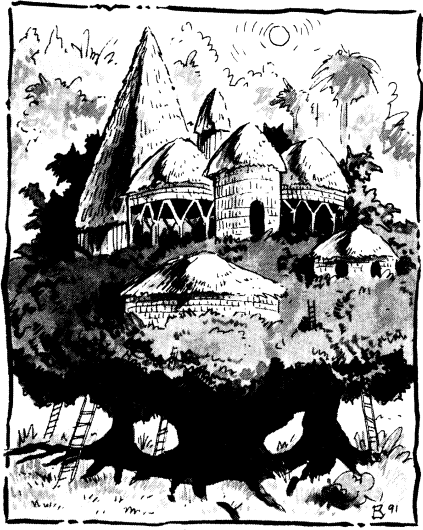
\includegraphics[width=\columnwidth]{images/gulg-1.png}
\end{figure}
\City{Gulg}
{13,500 (80\% humans, 7\% elves, 5\% dwarves, 3\% muls, 2\% half-elves, 2\% thri-kreen, 1\% other).}
{Agafari, copra, feathers, livestock, spices, textiles.}
{Common, Dwarven, Elven, Gulgan.}
{
	The city-state of Gulg sits inside the southern portion of the Crescent Forest, almost directly east of Tyr. Being east of the Windbreak Mountains, Gulg was spared the devastation that the Great Earthquake visited on the cities and villages to the west. That doesn't mean that life in Gulg has remained unaffected by the changes sweeping through the Tablelands. In a few significant ways, Gulg has been changed the most.

	Gulg's sorcerer-queen, Lalali-Puy (LE female champion of Rajaat stage III dragon, defiler 5/telepath 6/arch defiler 5/thrallherd 4/cerebremancer 5/Athasian dragon 2), is the absolute monarch of her realm. Her subjects consider her to be the Oba, the forest goddess. Over the centuries that she's been in power, Lalali-Puy has come to relish the worship and adoration her subjects heap upon her. In fact, though she remembers her origins as a Champion of Rajaat and a sorcerer-queen, she prefers to think of herself as the goddess her people believe her to be.

	To the Oba of Gulg, the abundance of rain---even the violent rain that accompanies a Tyr-storm---is a blessing to Athas. She has proclaimed this blessing to be a gift from the forest goddess. ``No longer will Gulg be solely concerned with the well-being of Gulg,'' the Oba declared to her people. ``Wherever the rain falls, there will the forest grow. And wherever the forest grows, the forest goddess will be there, for all the forests belong to the Oba.''

	Behind the rhetoric, Lalali-Puy actually wants to help restore the vitality of Athas. The Gulgs have always had an enlightened understanding of the interconnected nature of all life, so they've always treated the forest as a precious resource that must be maintained and not depleted. This attitude comes right from the Oba herself, which may seem strange as she is a defiler of extreme power. Since taking over Gulg, however, she has learned to temper her use of defiling magic in favor of keeping her forest healthy.

	Of course, this attitude was one of the contributing factors to the problems with Nibenay. The Nibenese saw the forest as a resource to be exploited, not a living thing that cares for its inhabitants as they care for it. Nonetheless, Lalali-Puy has made the first moves toward a peaceful existence with Nibenay, going so far as to teach the sorcerer-king how to preserve the life-giving environment of the Crescent Forest.

	The Oba's motivation isn't entirely selfless. She believes that when the forests return to Athas she will be deified by all races, just like she's been in Gulg. ``Let Nibenay and Hamanu play as sorcerer-kings,'' she has decided, ``for in the end I will be as a god to all of Athas.''
}
{
	The \emph{dagada} is the single most influential social force on Gulgs outside of the immediate family. The dagada is an extremely close-knit community that shares attributes of both clans and neighborhoods found in other societies. It is similar to a neighborhood in that it is a social organization defined first and foremost by physical proximity. It is like a clan in the role that it plays in acculturating an individual to the values of the society.

	The word dagada is used to describe both a cluster of huts and the people who live there. A dagada can contain up to 100 huts, and typically includes a number of families, though extended families may not necessarily live in the same dagada. Each dagada has a large degree of autonomy in managing its affairs as well as a degree of responsibility for all the members of the dagada. All parents have the burden of raising the young children of the dagada. Elders are responsible for educating the youths as they go. All members have a social duty to care for those who cannot provide for themselves.

	Life has always been more tolerable in Gulg than in any of the other city-states under the rule of sorcerer-kings. In some ways, life has actually gotten better for the Gulgs. The Oba's newfound crusade to restore Athas has made her more forgiving of and generous to her loyal citizens. In the spirit of cooperation, she has selected her best templars to travel the Tyr Region and spread the word of restoration. These templars have a twofold purpose. First, they help show the rest of the Tablelands how to work in harmony with nature, which Lalali-Puy hopes will hasten the reforestation of the world. Second, her templars pass along the tale that the rain is a blessing from the Oba, thereby increasing the number of people who know of and believe in Lalali-Puy.

	Except for the aid these templars have provided to Nibenay, no other city-state has thus far been targeted by the Oba's select force. Instead, the templars visit villages and oasis communities, teaching and preaching as circumstances permit. Some places have welcomed the templars, others have driven them away. Those communities that have actually experienced a Tyr-storm, for example, are quick to attack anyone who claims to be associated with their fearful properties, while those desperately in need of water invite them in.
}
{
\begin{figure*}[b!]
\centering
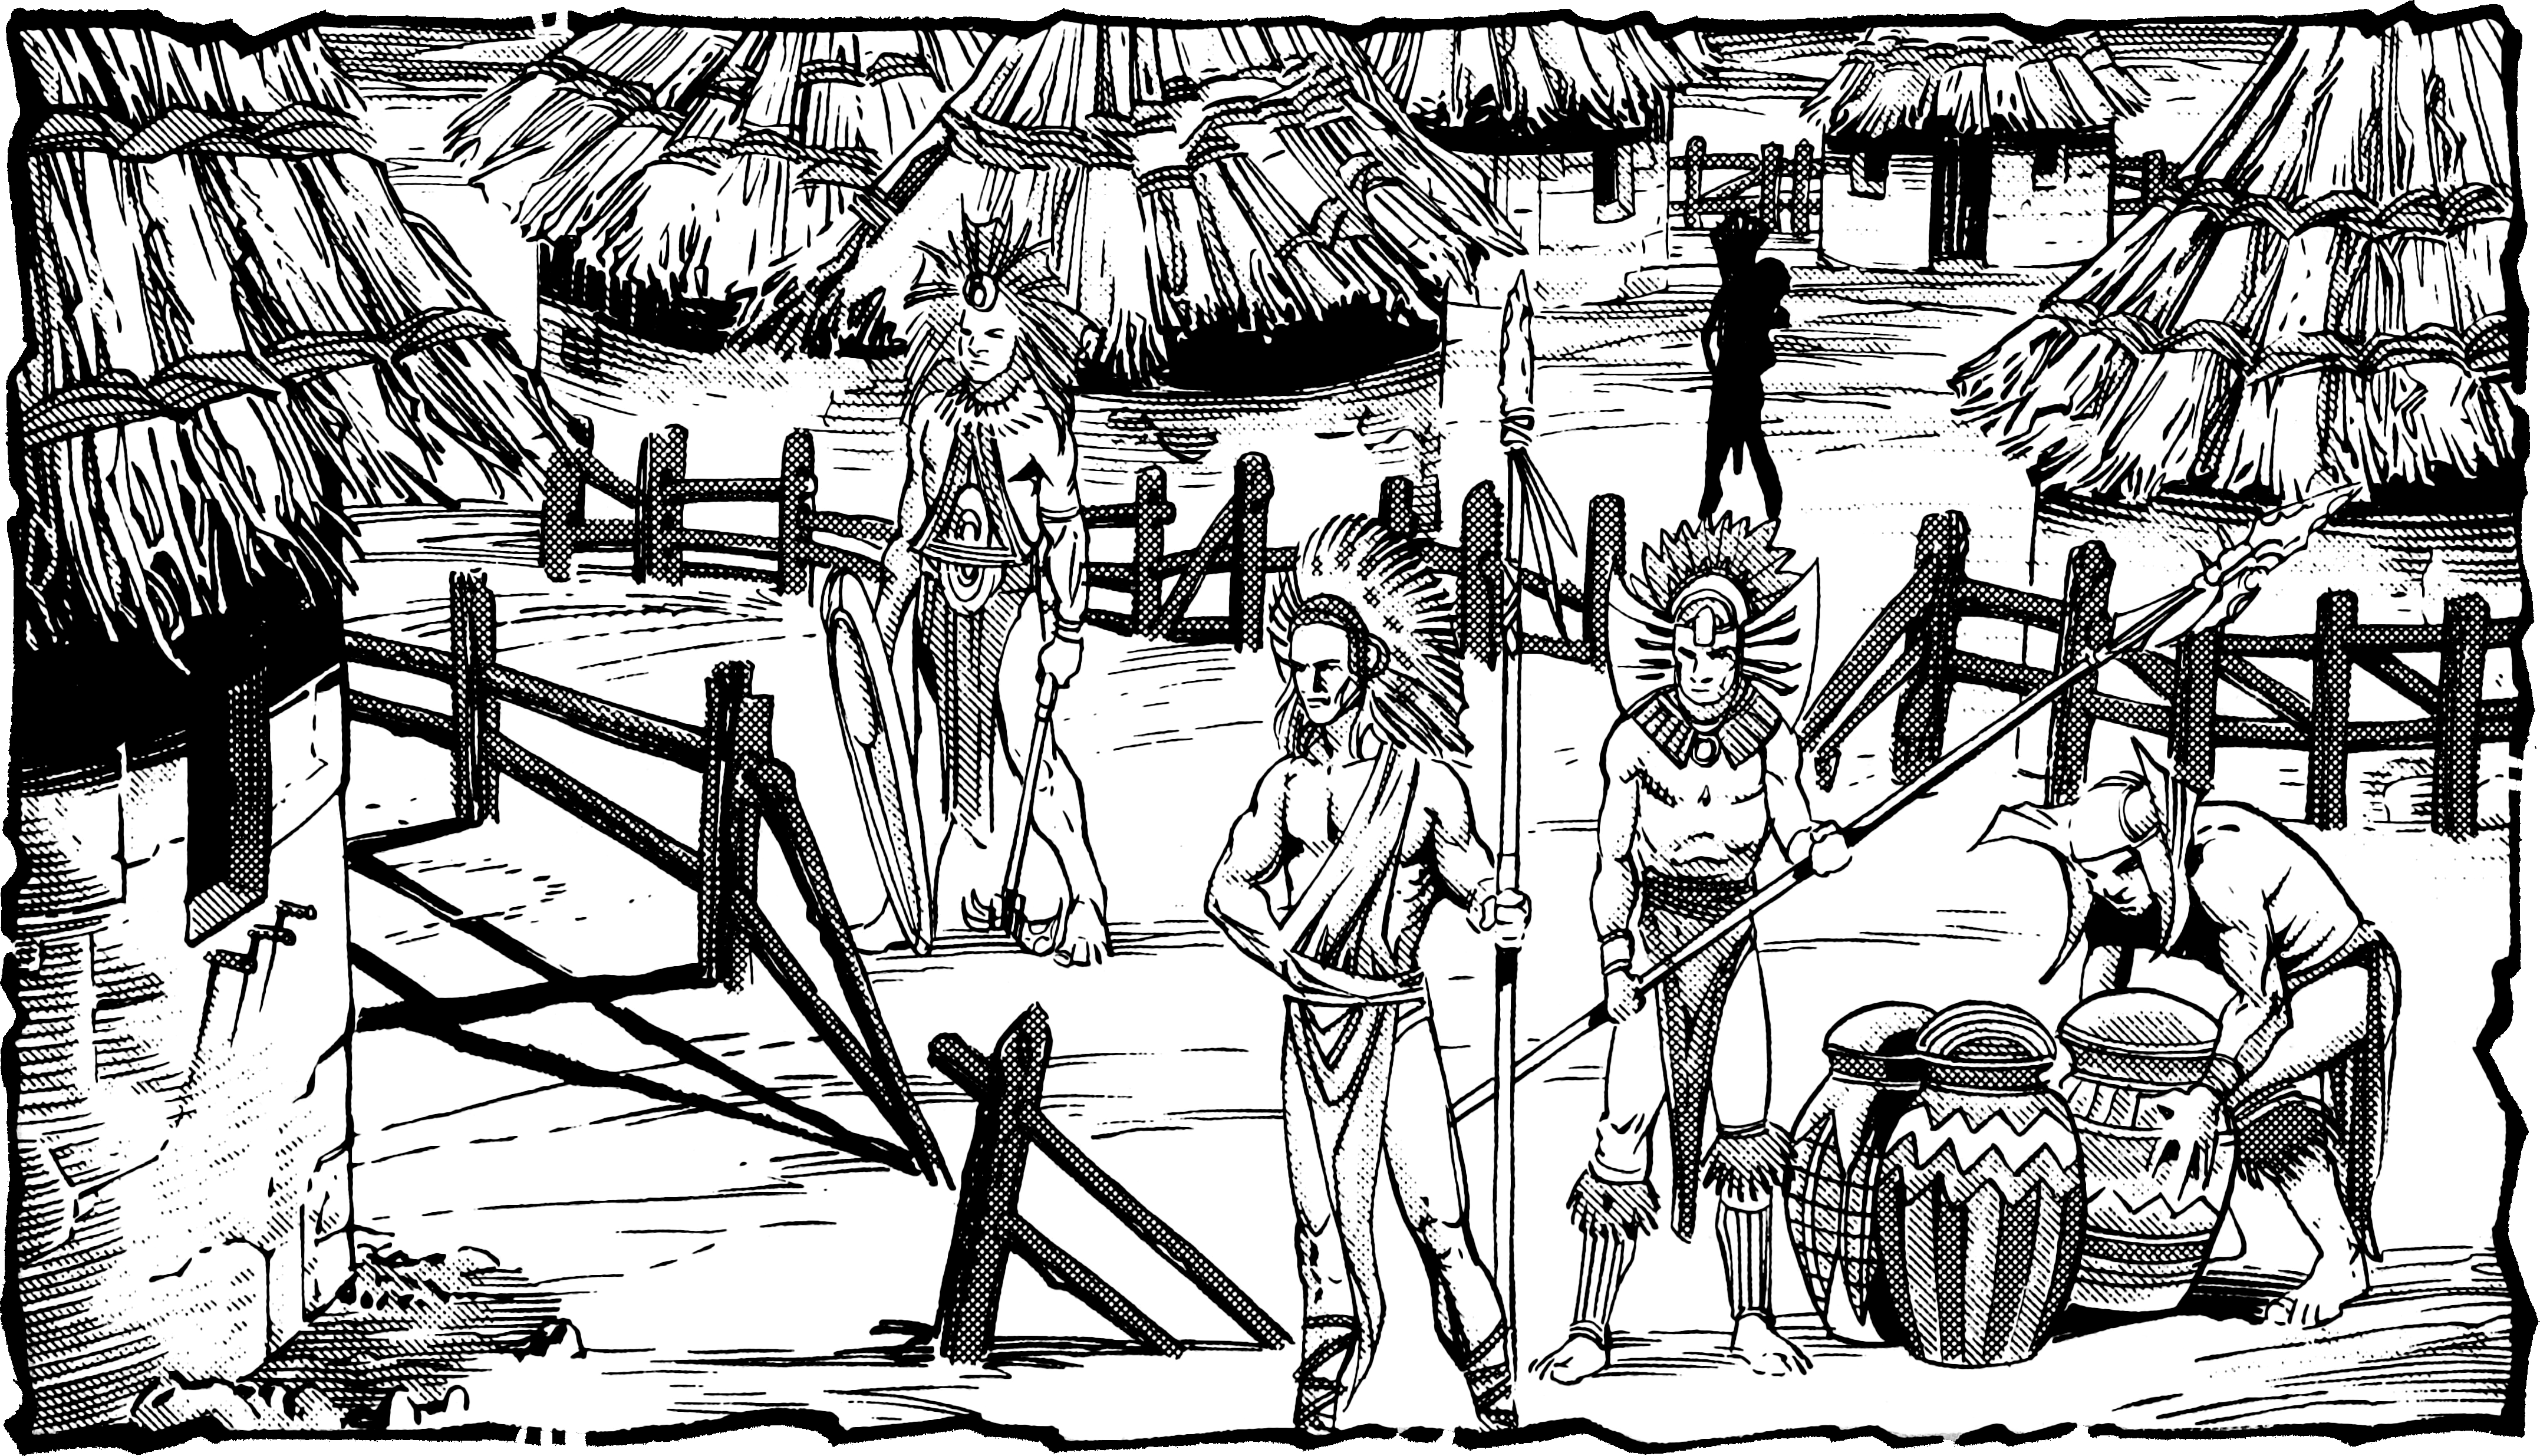
\includegraphics[width=\textwidth]{images/gulg-2.png}
\end{figure*}

	In many respects, Gulg is not like any of the other city-states of the Tyr Region. It's a living city, grown from vines and trees instead of constructed from brick and stone. The outer walls of the city, for example, consist of a thick hedge of thorny trees. The Oba lives in the tallest branches of a huge agafari tree, while her templars inhabit the lower branches. There are no paved or cobblestone roads leading through Gulg. Instead, forest paths and trails wind their way between the trees.

	There have been few major changes in the way Gulg is ruled. The Oba remains the owner of everything, distributing food, water, and other supplies to where they are needed most. Her templars continue to oversee the military, economic, and agricultural aspects of the community on behalf of the forest goddess. Nobility is still an earned position, not one granted by an accident of birth. The nobles hunt the forest for fresh meat, while slaves commanded by the templars gather the wild fruits, nuts, and berries that round out the dietary concerns of the community.
}
{
	\textbf{House Inika}: House Inika, the largest merchant family based in Gulg, is smaller than the typical merchant house. They specialize in small light weight goods of high value, such as spices, gemstones, and feathers from the exotic birds of the Crescent Forest. Inika maintains cordial relations with most of the other houses as it has a reputation for being nonconfrontational. Direct force is rarely used against rivals, with intrigue and economic means being the house's preferred means of strike back at rivals who try to take advantage of the house. The matriarch of the house is Andiama Inika (LN female human, rogue 14/ dune trader 5) who has ruled the house for more than two decades.

	\textbf{Judaga}: Nobility in Gulg is not granted by birth. Instead nobles must earn their position by proving they have the hunting skills necessary to provide meat for the rest of the community. There are several ways in which a citizen can become a noble. One of the most widely known ways a hunter can earn the rank of nobility is by participating in the Red Moon Hunt. During the hunt, prisoners are released unarmed into the Crescent Forest, and a thousand seconds later the hunters are sent after them. If a hunter returns with the head of the prisoners he has earned noble status, which will be bestowed upon him in a ceremony at the next High Sun. The Red Moon hunt is held on nights when the moon Ral is full and alone in the night sky.

	\textbf{The Paper Nest}: The Paper Nest is a secret society comprised of nobles favored by the Oba. The twelve to twenty-four members meet in a secret chamber in the trunk of the Sunlight Home to perform the sacred task of making paper. There is another reason for the group's existence besides making paper. Lalali-Puy attends the meetings and listens as the members debate current problems, offer advice, and present their counsel. At no other time does the autocratic Lalali-Puy allow her subjects to participate in the city's governance.

	\textbf{The Veiled Alliance}: A significant change in Gulg society concerns the Veiled Alliance of the city. Gulg's Veiled Alliance has always actively worked to restore Athas to its verdant glory, never directly opposing the will of the sorcerer-queen.

	Now that the Oba has declared her own intentions for restoring Athas, the two seem to have less to fight over. The Oba has even extended a ``peace leaf'' to the Alliance, calling for the preservers to shed the veil of secrecy and join the forest goddess's quest to save the world. The Alliance hasn't responded yet, but rumors persist that the preservers will soon come out of hiding in the forest city. The Alliance's leader, Aukash-Pad (LG male human, preserver 6/veiled one 5/earth cleric 3/psychic theurge 1), is utterly committed to restoring Athas' life force. If the Oba continues to genuinely work toward that same goal, he may be forced to join with her for the good of the world.
}
{
	\textbf{Losthome (Thorp, 60)}: Losthome is a halfling community deep in the Crescent Forest. The community is less than 10 years old and was formed when the Oba of Gulg attempted to form an alliance with a halfling tribe from the Forest Ridge. An agreement was made, but shortly after the halfling warriors arrived in Gulg, their chief died. The halflings believed that the death of their chief ended the agreement and sought to return to their home, but Lalali-Puy refused to let them go and imprisoned them. Over the years since, most of the halflings have escaped into the Crescent Forest and banded together around their leader, Zivlil (N male halfling, preserver 5/kineticist 3/cerebremancer 2). The halflings maintain no permanent settlement but roam an area of the forest approximately 40 miles wide, in which they have a number of prepared resting areas. The halflings wish to keep their existence a secret to convince the templars of Gulg that they died in the forest. So they kill any nonhalfling who sees them.
}
{
	\textbf{The Drum Circle}: The bard's quarter in Gulg is centered around a dagada called the Drum Circle. The bards of the Gulg specialize in percussion instruments. The most skilled bard in the Drum Circle is considered to be Ken-kenku Vek (NE male half-elf, bard 12). His skills as a drummer and an assassin are legendary.

	\textbf{The Forest Arena}: The gladiator arena of Gulg is located outside the city's mopti wall in the Crescent Forest. Trees and vines intertwine with the arena to give it the appearance of growing from the forest. The floor of the arena is oval shaped, and covered with grass. A number of trees grow from the arena floor; however, none is closer than 6 meters from the arena's walls, to prevent gladiators from using them to escape.

	\textbf{The Grove of Mysteries}: Throughout the forest surrounding Gulg there are a number of forest groves called the Queen's Groves. Entrance into one of these groves without the permission of the Oba is punishable by death. The Grove of Mysteries is the largest of the Queen's Groves and is tended by the druid Extambolan (N male mul, druid 5/grove master 10).

	\textbf{Mopti Wall}: Unlike the walls of other city-states, the walls around Gulg are alive. The Mopti wall is a miles long thorn wall make of thickly packed brambleweed that surrounds the city.

	\textbf{The Seers' Dagada}: When a Gulg shows psionic potential they are sent to the Seers' dagada, where they receive instruction from experienced psions. The teachers are patient and encouraging towards the students. Even those who fail to develop enough psionic potential are not cast out, but remain part of the Seers' dagada performing physical chores for the other members.

	\textbf{Sunlight Home}: Sunlight Home is the name given to the palace of Sorcerer-Queen, Lalali-Puy. Located in the tallest branches of a massive agafari tree, Sunlight Home towers over the rest of the city. Lalali-Puy's palace is rumored to contain dungeons and secret passages that have been carved into the trunk of the massive tree.
}
{
	\item Ngeli is a small boy of ten years old. While gathering cloves in the forest he was attacked and dragged off by a sloth. His parents are distraught and want to see a rescue attempt made to recover their boy, but the ambo of their dagada ruled that the boy was taken by the nature spirits and should be given up to his fate. Ngeli's parents turn to outsiders, the PCs, to secretly bring back their boy.
	\item The berry harvest has finished for the year. The berries had a strange brownish tint, but seemed fine to the taste. But those who have eaten too much of the berries have been having strange reactions. Some exhibit strange new psionic powers, others become sick and die, and some fall into a suggestive state and will do nothing but what others tell them to do.
	\item Alexia Vordon trades for spices with Gulg. She feels that her house trades at a disadvantage by being forced to deal with the templars. If she can make contact with a member of the spice gathers she is convinced that she will have a better understanding of how good the year's harvest has been and be in a better position to negotiate with the templars. Alexia hires the PCs to sneak her into the city and help her try to befriend someone from the spice gatherers dagada.
	\item Rumors in the neighborhood have begun that a teenage girl is really a witch. The wild rumors began when the girl started wearing a veil that covers her face leaving only her eyes showing. Many hot-headed, superstitious members of her dagada are contemplating drastic actions against the girl. The PCs will have to find some way to stop these rumors. The truth is that the girl has experienced her first heavy case of acne. Unsure of what is really happening to her, and fearful that others will reject her because of her affliction, she hides behind the veil, refusing to remove the veil and revealing her affliction to anyone.
	\item The PCs are invited on a hunt with a group of nobles from Gulg. The nobles seek to test the PCs hunting skills. They hang back letting the PCs take the lead, while hunting a dangerous beast, such as a klar.
	\item The templar, Kampala, has a feylaar as his fetish. When visiting a small client village, he summons the totem spirit, only to have it break from his control and go on a rampage.
}
\City{Nibenay}
{24,000 (60\% humans, 12\% half-giants, 10\% dwarves, 10\% elves, 4\% half-elves, 3\% muls, 1\% other).}
{Rice, timber, hardwood, weapons, copper.}
{Common, Dwarven, Elven, Nibenese.}
{
	Nibenay has been affected by the monumental happenings of recent months, for the Shadow King has changed his approach to ruling the masses and dealing with the neighboring city-states. Like Hamanu and Lalali-Puy, Nibenay (who shares the same name as his domain) witnessed the deaths of the Dragon and the other sorcerer-kings.

	He saw Rajaat reach out from beyond the veil of Athas to wreak vengeance against those who betrayed him. He also saw Rajaat defeated by the efforts of lowly mortals from the city of Tyr. In the wake of these signs and portents, Nibenay realized it was time to reconsider how best to rule his city, for the time for change had come.

	The city-state of Nibenay is located east of Tyr at the northern tip of the Crescent Forest. It barely felt the effects of the Great Earthquake, as it was protected by the Windbreak Mountains. Nibenay has also thus far been spared from Tyr-storms and the growing unrest spreading throughout the Tablelands. If the Shadow King has his way, none of these problems will ever reach his domain.
}
{
\Figure{b}{images/nibenay-1.png}

	Though there have been no major changes to life in Nibenay, enough strange occurrences have been worked into the routine to put a different spin on the city-state. For example, average citizens and even powerful nobles never expected to see the Shadow King, let alone attend one of his courts. Now the Shadow King regularly makes public appearances and shows an active concern for his community. This doesn't mean that life is any harder or easier than it's always been. It's just different. If a citizen or visitor breaks a law and can't afford to bribe a templar, then that citizen or visitor is still going to end up in Nibenay's slave pens.

	The other major change is the city's outlook on matters of a martial nature. The Shadow King and his templars seem to be concentrating much of their efforts on bolstering Nibenay's military might. The army regularly practices in the arena and patrols of the surrounding countryside have increased dramatically. In addition, free citizens and nobles have been ordered to serve in Nibenay's defense. Templars are busy organizing them into part-time militias and regimenting training sessions.

	What the Shadow King is truly concerned about, besides the unrest and upheaval that seems to be spreading throughout the Tablelands, are the rumors claiming that Dregoth has returned. Nibenay knows how powerful the sorcerer-king of Giustenal was. Dregoth was second only to Borys the Dragon in power. If Dregoth and his city have somehow come back from the dead, Nibenay wants to be prepared.

	After all, Nibenay's city-state is one of the closest to the ruins of ancient Giustenal, and he has no intention of losing his domain to a rival that was destroyed two millennia ago.
}
{
\Figure*{b}{images/nibenay-2.png}

	The sorcerer-king Nibenay (LE male champion of Rajaat stage IV dragon, defiler 5/seer 5/loremaster 10/cerebremancer 10/Athasian dragon 2) used to stay behind the scenes. He was called the Shadow King because he rarely left Naggaramakam, his walled sub-city. His templars, who are all female, ran the city with skill and great care. Now, however, the Shadow King has become more prominent.

	In the past, the average free citizen could hope to see King Nibenay once or perhaps twice in an entire lifetime. Since the time of the Great Earthquake, Nibenay has taken a more active role. He still allows his templars to deal with the daily business of government, but now Nibenay has turned his attention away from the mysterious scholarly pursuits that once occupied his time to hold court for the city's nobles and free citizens.

	Nibenay's military might was never a question, but it also was never a major concern of the Shadow King. Now he actively seeks to understand his forces and looks for ways to improve their might and readiness. While the city used to appear to be secure in its own position, it now seems to be gearing up to battle an enemy that only the Shadow King knows about. The problem is that the enemy is change, and no army that Nibenay raises will be able to stop its relentless tide.

	In the wake of all this upheaval, Nibenay's nobles continue to care for and maintain the bubbling springs that surround the city. They don't know what to make of the Shadow King's sudden interest in the business of the city, but many of them are seeking ways to improve their own positions by getting closer to their once-elusive king.
}
{
	\textbf{Poortool's Horde:} Lead by the half-Elven preserver Poortool (LN male half-elf preserver 5/seer 3/cerebremancer 5), the Horde is a raiding tribe to the east of Nibenay. Poortool is a renegade from the Veiled Alliance who seeks to study magic without any restriction that the Veiled Alliance or sorcerer-king Nibenay may apply. He has created a community for likeminded preservers in a village in the foothills of the Black Spine Mountains. He has also allied with the gith of the Black Spine Mountains who provide guards and raiders for his tribe. Poortool seeks to make it difficult for members of the Veiled Alliance in Nibenay to convince its members to leave the Alliance and join him.

	\textbf{House Shom:} House Shom is thought to be the oldest merchant house operating in the Tyr region. For centuries the house amassed great wealth through aggressive trading. However, now the House is seen as passive and decadent. The Shom family members are almost never seen in public and have little to do with the daily business of the house. Instead the family members live decadent lives in their palaces, engaging in expensive parties and balls. The running of the trading house is left to the house agents. Most of the agents place their interests ahead of House Shom's interests, and there is much infighting between agents. This has lead to a decline in the House's prospects over the past few decades. Only the house's immense wealth has saved it from collapse already. House Shom is known to use non-human guards on its caravans and as raiders against other merchant houses, including thri-kreen packs and belgoi tribes. The house is currently ruled by Temmnya Shom (NE female human, defiler 15). Her younger brother, Jebea Shom (LN male human, rogue 3/fighter 2/dune trader 1) has begun a reform movement to straighten out the family's problems, but his popularity threatens Temmnya's position. She has contemplated disposing of him if she can do so without her involvement being discovered by other family members.

	\textbf{Sky Singers:} The Sky Singers elf tribe maintains a permanent market in the Hill District of Nibenay. It is the only known instance of a permanent Elven market. The market is filled with goods of all kinds from the rare to the common. The Sky Singers have a reputation of offering quality products that were not stolen from their previous owners, unlike most Elven tribes. While the tribe numbers over 3,000 members, much of the time the elves are off wandering, leaving only a dozen or so elves to tend the marketplace. But when the tribe returns, the Sky Singers' market takes on a festive atmosphere.

	\textbf{The Veiled Alliance:} Nibenay's Alliance has an utter hatred of defilers. This has led to a rare commodity beneath Athas' crimson sun-idealism. With the help of an ancient spiritual force known as the zwuun, which resides in the hot springs outside the city, the Alliance does what it can to protect wizards who use preserving magic. The Alliance doesn't feel it can oppose the Shadow King directly, so it directs its activities against lesser defilers. Thagya Phon (LN male human, preserver 7/veiled one 10) leads the Nibenese Alliance, though his health has begun to fail him in recent years. He has two goals he wishes to accomplish before he dies: He longs to discover what Nibenay's scholar slaves have been working on in the Naggaramakam, and he has a dream of mounting the Shadow King's head on the obsidian pedestal that rises from the floor of his spartan quarters.
}
{
	\textbf{Cromlin (Hamlet, 150):} The trading village of Cromlin sits on the shores of the Silt Sea, northeast of Nibenay. House Shom runs the village, though House M'ke has a sizable operation as well. Together they handle the vast majority of trade from the north, as traders attempt to bypass the chaos of Raam. Cromlin traders use silt skimmers to navigate the silt shoals, keeping the trade route to Break Shore open. The shoal navigators of Cromlin are in high demand, for they are among the select few who can lead silt skimmers along the buried paths.

	Cromlin is a wild place, full of people who are too untamable to live in the cities. Thieves of all sorts reside in the village. Silt pirates use it as a haven and other scoundrels and restless souls are drawn to its sandy shores. Master trader Hurdll Crost (N male human, bard 10/dune trader 5) and his agents turn a blind eye towards shady characters as long as they remain to do business in his village.

	\textbf{Salt View (Small Village, 550):} Nestled in the Mekillot Mountains, Salt View is a chaotic sprawl of tents and buildings located within a large cavern on the mountain's eastern face. Ex-slaves of all races fill the community. The tribe originally practiced raiding as its primary occupation, but today it is known for a lavish form of storytelling called theater. Salt View's traveling theater troupes are welcome across the Tyr Region, though they present themselves as free merchants from the independent House Fyra (a cover for Salt View activities). The troupes perform for caravans, at oasis villages, and even in the city-states of Tyr, Nibenay, and Balic.

	\textbf{Vavrek (Thorp, 200):} Vavrek is typical of the small farming villages located throughout the Fertile Crescent. The village is located southwest of Nibenay within sight of the Crescent Forest. The villagers grow vegetables, mostly soybeans. The land the village is built on is owned by the Koelse noble family, to which the villagers must pay rent. The village is administered by a templar-wife of Nibenay named Sonyalah (NE female human, templar 5/wife of Nibenay 3).
}
{
	\textbf{The City Reservoir:} The Shadow King had this enormous stone cistern constructed centuries ago to supply the city with water in the event of a siege. The top of the reservoir is covered and a lush garden, maintained by the templars, grows on top of the reservoir.

	\textbf{The Coliseum:} The coliseum rises above the dilapidated buildings in a rundown part of the city. The size of the arena is immense, taking up four city blocks and rising six stories high. It is an ancient building and it is said that not even the Shadow King knows when the coliseum was built and by whom. Elaborate carvings and etchings cover the coliseum's stonework. The square shaped arena floor stretches almost a quarter of a mile across.

	\textbf{Monasteries of the Exalted Path and of the Serene Bliss:} Nibenay has a tradition of monasteries. The two orders are called the Exalted Path and the Serene Bliss. The monks pledge loyalty to the King and their teachings include the quiet acceptance of authority, so the templars tolerate them. They are treated with great respect by the citizens. The monks live very aesthetic lives, tending gardens and mediating. Many of the monks, especially those of the Exalted Path, study psionics. The Exalted Path consists entirely of male monks and is led by Thong Nal, (CN male human, air cleric 3) who encourages the study of psionics at his monastery. Other monks become artisans who specialize in the carving of the images that cover the buildings of Nibenay. The Serene Bliss is an all female order and is led by the abbess Au Treng (LN female human, cleric 4).

	\textbf{Naggaramakam:} The Naggaramakam is a walled forbidden inner city where the sorcerer-king Nibenay lives with his templar-wives. Only templars are permitted to enter and leave the Naggaramakam. While slaves are permitted to be brought into the Naggaramakam, once inside they are never allowed to leave. No free citizen is ever allowed to see the inside of the Naggaramakam. The sorcerer-king's palace is said to be carved into a stone relief of the Shadow King with dancing women, representing his templar-wives, strung together as if they were his hair.

	\textbf{The Omnipotent Receivers:} A line of large statues of sorcerer-king Nibenay stand on each side of the main road leading to the city. The statues are called the Omnipotent Receivers as it is believed that King Nibenay sees all that the statues see.

	\textbf{The Plain of Burning Water:} The city of Nibenay is situated on the border of a large area of hot springs. Called the Plain of Burning Water, the hot springs provide the water needed by the citizens of Nibenay. Each noble house owns at least one of the hot springs which is the source of much of the wealth of the nobility.

	\textbf{Sage's Square:} Sage's Square is the largest open area inside of the city. The grand emporiums of all the dynastic merchant houses are located around the square and are the center of trade in Nibenay, where almost anything can be purchased. The square was named Sage's Square because scholars and sages use to gather under the shadow of the huge agafari trees that grew in the square, and debate philosophy. This tradition ended only a few years ago when a renegade defiler, fleeing the templars defiled the trees. King Nibenay had the dead trees removed from the square, and ordered that no other trees be planted in the square as a public reminder of the danger of renegade defilers.

	\textbf{The School of Augurs:} The school of Augurs is the largest school for psionic instruction in Nibenay. The head master is a dwarf named Djef, who developed a scheme to help support the school by hiring out its students to transfer telepathic messages and to teleport-deliver small parcels.
}
{
	\item A disguised dray agent has entered Nibenay seeking to make contact with nobles disgruntled with the Shadow-King's rule. The dray tries to gather together as many nobles as possible so that when Dregoth makes his attack on Raam, he can start a rebellion in Nibenay to distract the Shadow-King from interfering in Dregoth's plan.
	\item The templars attempt to ambush a cell leader of the Veiled Alliance who they believe is staying at the same inn as the PCs. During the templar raid, one of the PCs is mistakenly identified as the Veiled Alliance member. Capture means execution, so the PCs must flee. If the PC makes it out of the city, his problems are not over. Because of the secrecy of the Veiled Alliance, the subordinates of the cell leader have never met him before. When the templars identify the PC as the cell leader, the other members assume it to be true. When the PC flees the city the cell members attempt to enforce Requital, believing the PC has tried to resign from the Veiled Alliance.
	\item Ramai is a templar of Nibenay, who is responsible for interrogations. Dedicated and highly skilled in all manner of interrogation and torture techniques, she holds some respect within the templar hierarchy. Her career appeared promising until one day, inexplicably, Ramai fell in love with one of her victims, a young man named Tongkol. Unable to bear the thought of Tongkol suffering under torture but also realistic enough to know they can never be together, she assigns the PCs the task of spiriting Tongkol out of the city. Ramai will not offer the PCs any direct help, but can give them information to help them succeed. If the PCs fail and are captured, Ramai will deny any involvement with the PCs and see that they are executed quickly to silence them.
	\item Gith raiders have discovered a previously unknown ancient catacomb that allows them to enter the city undetected. They raid some dwellings in the city and attempt to flee back the way they came. But undead that were angered by the gith's trespass have arisen and prevented the gith from getting out of the catacombs. The PCs are sent into the catacombs after the gith and must also face the undead horrors.
	\item One of House Shom's merchant forts has been overrun by gith. The PCs are hired to lead the assault to retake the desert fortress.
	\item A preserver of the Veiled Alliance asked the zwuun for help on his latest research. The zwunn's answer directed the preserver to the site of ancient ruins that overlook the road to North Ledopolus where he could find what he sought. Unsure if the zwuun was being mischievous or not, the preserver sends the PCs to scout out the ruins.
}
\begin{figure}[b!]
\centering
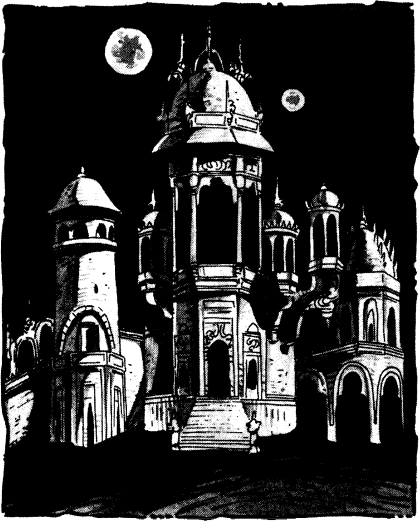
\includegraphics[width=\columnwidth]{images/raam-1.png}
\end{figure}

\City{Raam}
{40,000 (40\% humans, 20\% dwarves, 15\% elves, 10\% muls, 5\% half-elves, 5\% half-giants, 4\% thri-kreen, 1\% other).}
{Silver, gems, flint, jute, silk, textiles.}
{Common, Dwarven, Elven, Raamite.}
{
	Shortly before the day of the Great Earthquake, the sorcerer-queen Abalach-Re was killed in battle with Sadira of Tyr. When the news reached Raam, it was the spark that ignited the fires of anarchy, and now Raam burns. But Raam was a city on the brink of revolution even before the death of its queen. Since Abalach-Re's death, the city has collapsed into chaos. Various factions have grabbed whatever power they could, and Raam teeters on the brink of civil war.
}
{
	Raamish society revolves around a caste system. Each citizen is born into a caste and can never leave it. Members of one caste cannot marry or associate with others from another caste without becoming unclean. Caste and race are not related, and a member of each race can be of any caste.

	The highest caste is made up of priests. This caste includes clerics and druids, as well as teachers, scholars and wise men. Members of this caste wear white garments to distinguish themselves.

	Below the highest caste, is the vizier caste. The templars and soldiers of Abalach-Re fall into this caste. The members of the vizier caste typically wear silk clothing dyed a variety of colors.

	The next caste includes the majority of the nobles of Raam, as well as artisans, and tradesmen. Wealth has no affect on one's caste. The richest tradesmen will never rise above his caste. This caste typically dresses in clothing made of less expensive material than the silk worn by the vizier class.

	The laborers caste is the largest caste and the lowest. It includes all servants and unskilled workers as well as the vast numbers of slaves. Laborer caste members wear simple white linen clothing.

	Below the laborers caste are the truly desperate. Outcastes are those who most handle dead animals and people. Butchers, morticians, and tanners are all included in this caste. They are considered so unclean that they must live outside the city to prevent them from polluting the rest of the citizens.

	The environmental disasters of recent months have had very little impact on Raam. The Great Earthquake was barely perceived, for it caused little damage and no deaths. No Tyr-storm has yet visited the city-state, so Raam's residents have yet to experience the devastation that such a storm can inflict. The death of Abalach-Re and the resulting struggle for power, however, have caused more death and destruction than any force of nature.

	Raam has been divided into armed camps controlled by greedy, power-hungry warlords. Some call themselves templars, others nobles, liberators, or merchant lords. All are raiders and bullies, seeking to use strength as a means of control.

	These armed camps don't even make a pretense of peaceful coexistence. Skirmishes over disputed territories are constantly being fought, as are battles over caches of weapons or supplies-even just to determine which side is stronger! It won't be long before all-out war breaks out to see if one leader and his faction can conquer the others and restore order of some sort to the city. This war, of course, may simply wind up destroying Raam and reducing the verdant belt it occupies to a wasteland.

	Understandably, the free citizens live in a constant state of fear. They have nowhere to go, nowhere to turn to, and conditions within the city become more terrible every day. Some citizens have appealed to one faction or another, offering to become indentured slaves for the protection and sustenance offered by the vying warlords.

	Every day, more and more citizens surrender their freedom in exchange for a safe place to sleep, a cool drink of water, and a bit of food to fill an aching stomach.

	The slaves of the city have fared even worse than the free citizens. Their masters have been replaced by heartless owners who treat the slaves no better than living tools that can be replaced when they break. Some slaves, embracing the legends of Rikus, Neeva, and Sadira of Tyr, have rebelled, using the opportunity presented by the chaos. One group has come under the leadership of a gladiator named Korno (CN male mul, barbarian 1/gladiator 4/arena champion 4). Between Korno's military daring and expertise and the cache of weapons his followers found in one of Abalach-Re's many hidden treasuries, this group of slaves has set itself up as another armed band in a city of gangs. Korno has called for all slaves to join his community, for when they have the numbers to go along with their dreams they will rise up and overthrow all their masters. Korno, however, is as cruel and ruthless as any of the other leaders of the armed bands. The slaves that have flocked to his side continue to be treated as slaves, working to make life easier for Korno and his best warriors.

	With food and water in short supply and violence rampant in the streets, it is little wonder that the people of Raam are turning to anyone or anything that claims to have a solution. In this volatile environment, revolution seems to be inevitable. What the outcome of such an event will be is unknown, but by all indications it will be bloody in the extreme.
}
{
\begin{figure*}[b!]
\centering
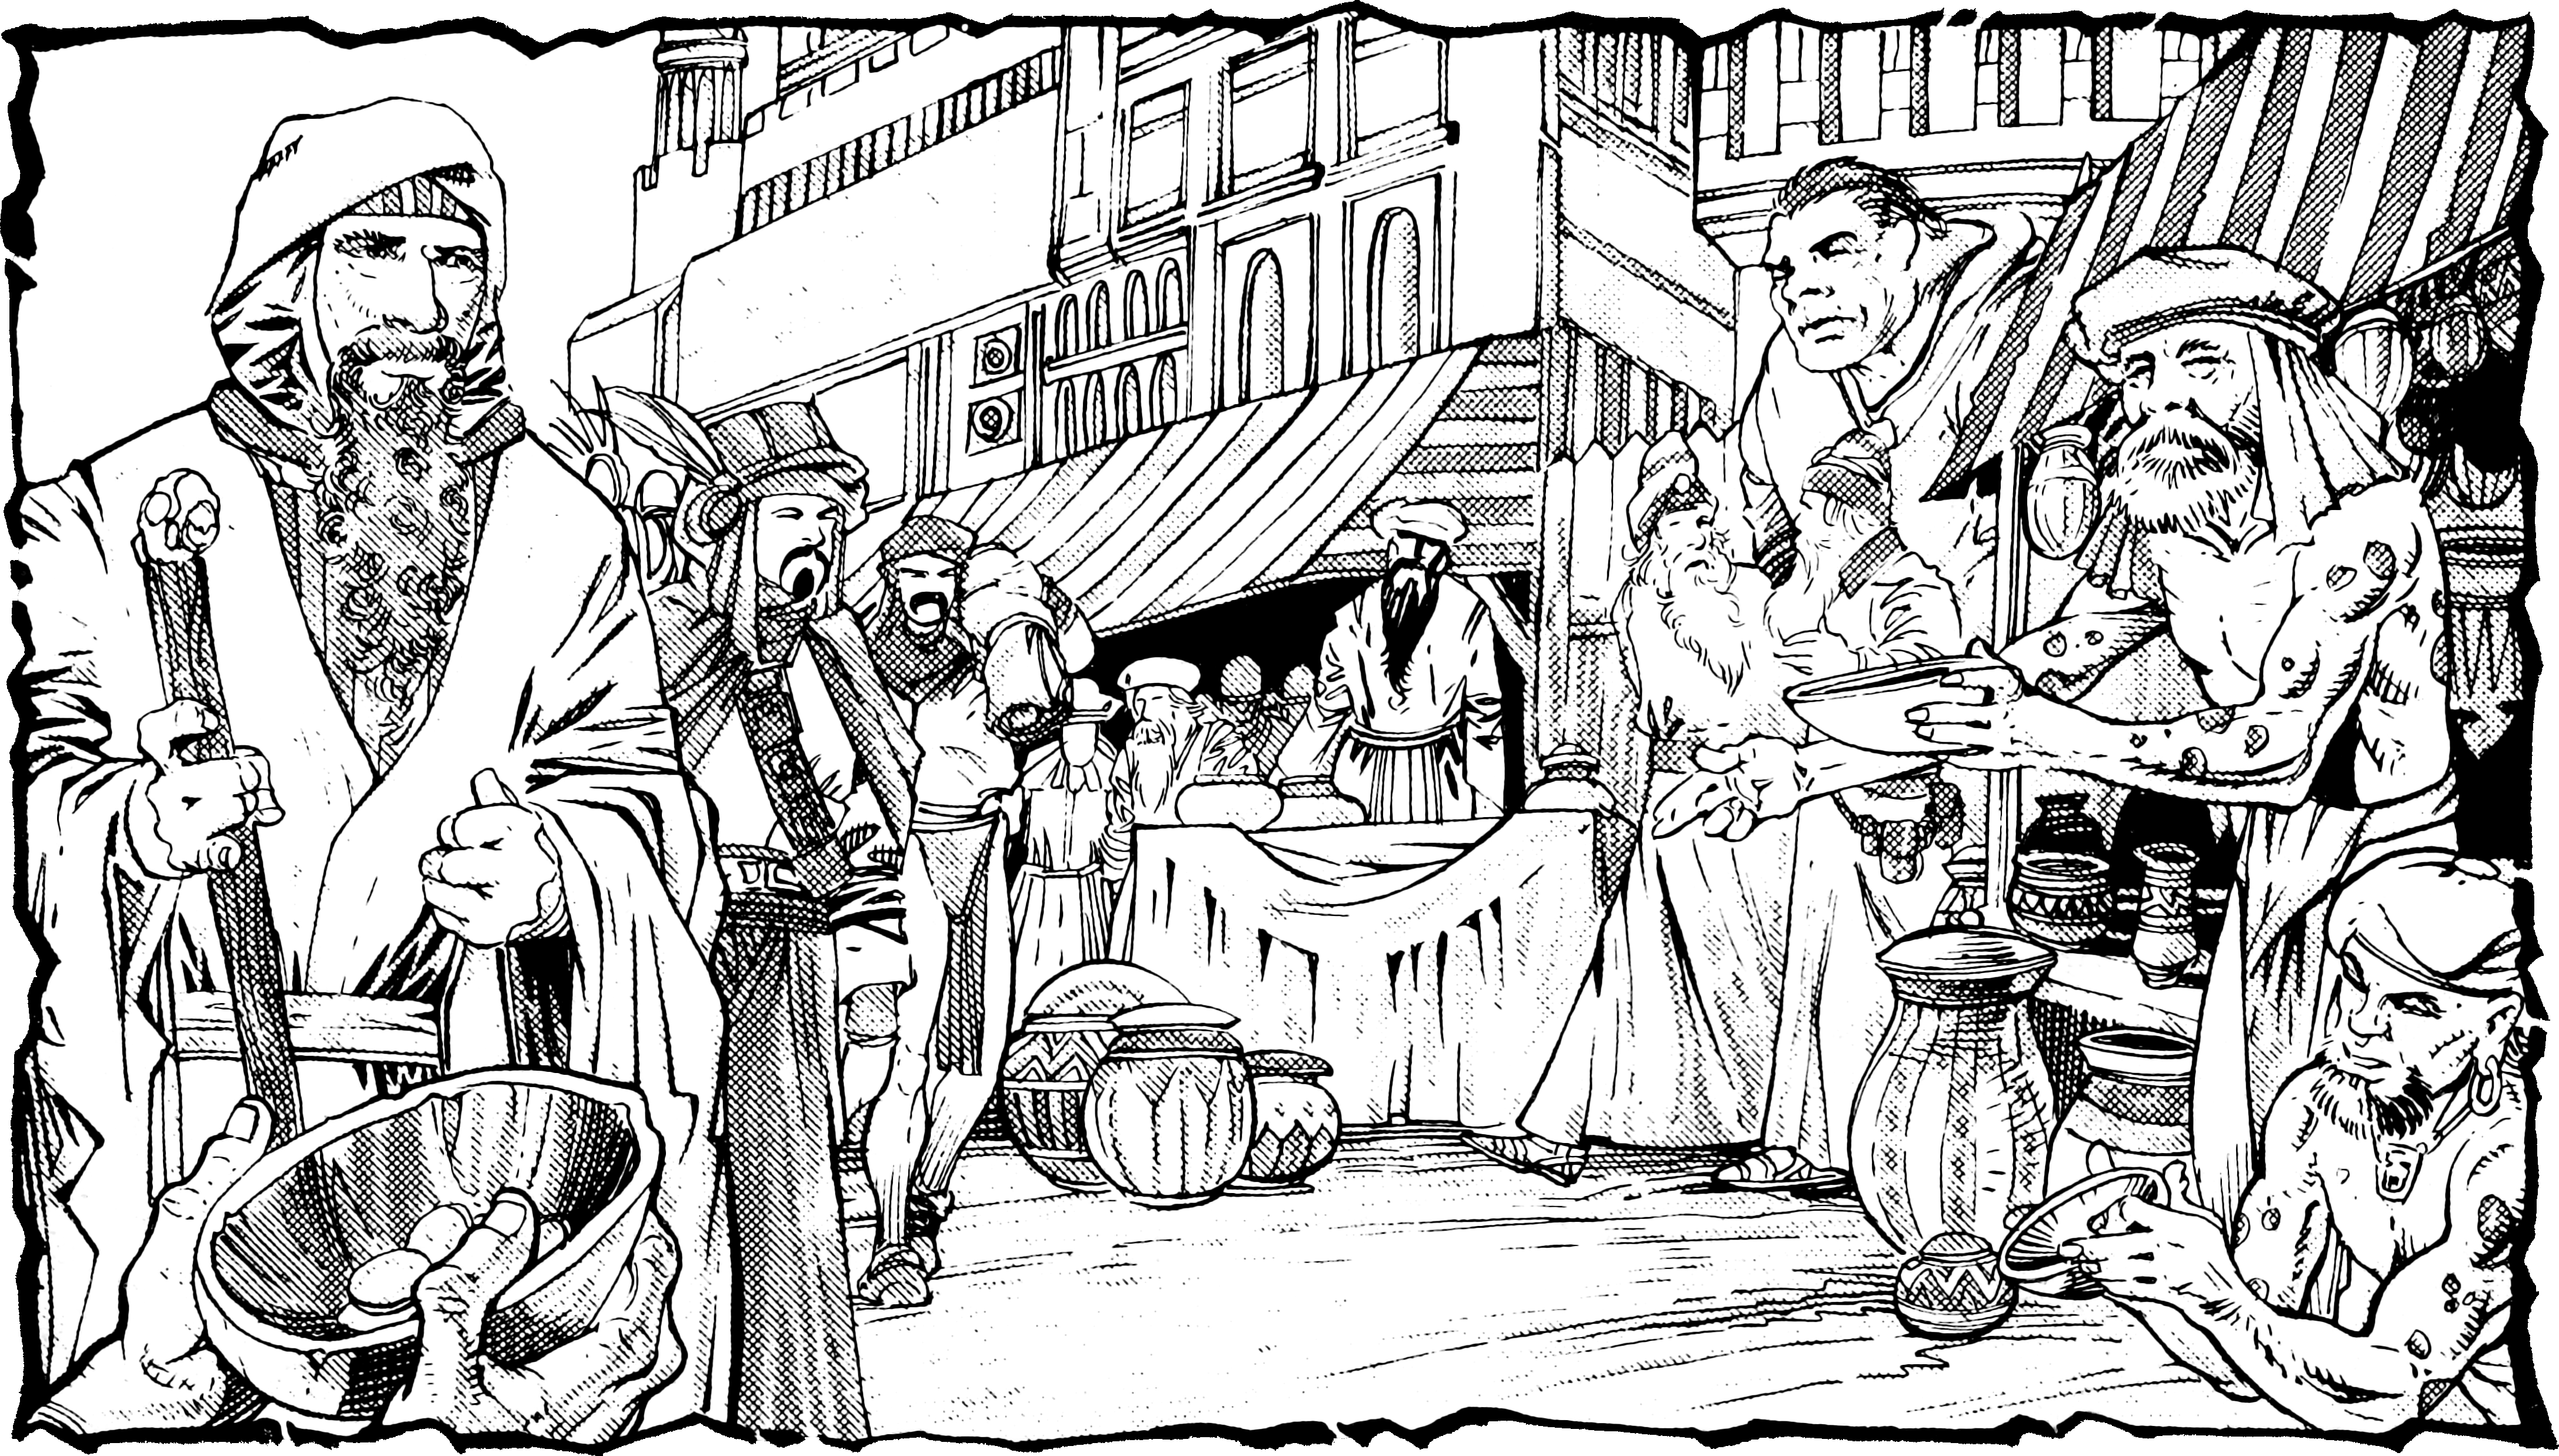
\includegraphics[width=\textwidth]{images/raam-2.png}
\end{figure*}

	The government of Raam still exists, but it has almost no power in the face of the violence and chaos ravaging the city. The templars who haven't fled in fear or tried to hide among the populace as regular citizens continue to administer the city, but it is clear the city no longer functions the way it used to. These templars have only their bureaucratic skills to fall back on, as their ability to use priestly spells vanished with Abalach-Re's demise. The templars continue to call for the worship of Badna, the mysterious (and imaginary) being the sorcerer-queen claimed to receive her powers from. Most people ignore these calls to worship, for they never believed in Badna anyway.
}
{
	\textbf{Leviath the Calm}: Leviath the Calm (LN male half-giant, shaper 9) is an unusual half-giant who speaks of peace and tranquility to all who would listen. His words are spoken with kindness and sincerity, and have had a profound effect on the masses, among which he has developed a large following. Despite his large size and strength Leviath is said to have never raised his voice in anger or struck a blow to harm another living creature.

	\textbf{House M'ke}: The merchant houses have taken one of two tacks regarding conducting business in Raam. The first option, chosen by the vast majority of merchant houses, was to get out of town and take their business elsewhere. The second option, embraced by House M'ke as a prudent enterprise that will ensure its own survival, was to seize control of as much of the city as possible. House M'ke and its army of mercenaries now control most of the merchant district. Armed bands wearing House M'ke's colors periodically sweep through the city, looting and pillaging until they gather enough goods to fill a caravan. This caravan then sets out across the Tablelands to conduct trade as any merchant house caravan would. Only in Raam does House M'ke behave like a conquering army of raiders-because in Raam, that's what House M'ke has become. A few of the more daring (or desperate) merchant houses return to Raam from time to time to test the climate, but they usually wind up losing their goods to one or more of the armed camps seeking dominance in the city.

	\textbf{Night Runners}: The strangest group to stake a claim in Raam's power vacuum is the elf tribe known as the Night Runners. Prior to Abalach-Re's death, the Night Runners maintained a small presence in Raam. Now this group of elves-which specializes in the ``shadow arts'' of espionage, assassination, and extortion-has decided to take a more active role in Raam society. A large portion of the elf quarter and the tradesmen's district has been taken over by the Night Runners. Besides holding and expanding their own territory, the Night Runners continue to sell their unique services to those who can afford them---including noble houses, merchant camps, and even templar domains. In the end, the Night Runners plan to control the entire city, making it the first elf city in thousands of years. Until then, the elves don't mind working for the bands they're competing with, for it gives them an easy way to keep tabs on how the factions are doing.

	\textbf{Nobles}: One of the largest groups claiming dominion over sections of Raam is the noble families. Like the raiding tribes of the sandy wastes, the nobles pillage and plunder for the things they want and need to survive. The nobles have expanded their areas of control. While each family started with a small piece of land and the road adjoining it, those with the power and audacity to press their advantage have grabbed whatever they could hold onto. Like the raiding tribes, the noble camps are savage, ruthless, and have only their own interests at heart.

	\textbf{Prophets of Dregoth}: Strange figures with bizarre accents who hide their features beneath many folds of robes preach of Dregoth the Savior. These prophets claim Dregoth is a god who will bring salvation to Raam if they lay down their weapons and accept him.

	\textbf{Templars}: The main body of templars occupies one camp, centered in the templar quarter of the city. Various rogue templars command smaller parts of Raam, claiming from as little as one building to as many as several blocks as their personal domains. They defend these domains with troops that were once loyal to Abalach-Re but now follow their templar commanders.

	Under Abalach-Re's reign there were two organizations of templars assigned to police the city. The mansabdars were the public force. They were assigned to guard and patrol duties. Though the larger of the two police forces, the mansabdars were corrupt and many were incompetent. The kuotagha was the secret police force. These ruthless enforcers were tasked with administering justice as they saw fit. Disguised as merchants and artisans, they moved freely among the population spying out sedition and unlawful behavior. When they judged someone guilty, the kuotagha executed the suspect without trial, immediately and by surprise. All kuotagha members carried a special garrote called a ghi, for use in such situations.

	\textbf{The Veiled Alliance}: The turbulent conditions in Raam haven't made it any easier for the city's Veiled Alliance. The preservers continue to operate in secret, but the contacts they once had in all levels of government have been lost. Nanda Shatri (LG female human, preserver 7/telepath 4/veiled one 10) continues to lead the Alliance and still seeks to become an avangion so that she can help restore Athas' lost vigor. However, beyond the vague rumors that Urik's Alliance had created such a being some years back, Shatri is no closer to her goal than she was a decade ago. She has considered siding with one of the armed bands in order to assure the safety of her people, but she has yet to determine which band to approach. Her reluctance to make a decision might be her undoing, for the Prophets of Dregoth have begun making overtures to the Alliance that the members find very appealing. In fact, the Prophets have also promised that Dregoth can help Shatri with her research into the avangion transformation process---a promise that she is seriously considering accepting.
}
{
	\textbf{Daro (Thorp, 300)}: Daro was a center of agricultural administration, used to oversee the slaves working the fields of Raam. After the death of Abalach-Re, templar Avish Thira seized control of Daro, instituting martial law which prevented the chaos that swept the rest of the city-state from reaching Daro. Under Avish Thira the village no longer is concerned with agriculture. The fields have been allowed to become fallow and most of the hundreds of field slaves have been freed, actually expelled from the village since Thira could not feed them. Thira supports himself and his guards by sponsoring raids into Raam.
}
{
	\textbf{The Benevolence Center}: The Benevolence Center is the name of a large housing complex for the elderly.

	\textbf{The Consecrated Sepulcher of Badna}: The massive Consecrated Sepulcher of Badna is one of the most majestic buildings in Raam. The Sepulcher is a mausoleum where the remains of the last 30 generations of favorite husbands of sorcerer-queen Abalach-Re were laid to rest.

	\textbf{The Crematory}: The stark granite walls of the Crematory tower over the slums outside the western wall of Raam. There are no windows in the entire building. A large chimney rises from the back of the building, emanating a thick column of smoke. Only outcastes are considered suitable to handle the remains of the dead, and as such the crematory is staffed completely by outcastes. Members of the rest of Raamish society spend as little time as necessary in the Crematory for fear of being contaminated.

	\textbf{The Gallery of the Seven Stars}: The Gallery of the Seven Stars houses the works of Raam's finest sculptures. Built of white rock, the Gallery is decorated with ornate murals and minarets. The museum contains seven star-shaped display halls where magnificent sculptures are displayed.

	\textbf{Natural Arena of Raam}: Raam's gladiator arena is a naturally formed amphitheater formed between two hillocks, outside of the city's walls. Wind and time have carved one of the hillsides into natural seating areas of rust colored rock. The arena floor is a rough oval and has a floor of red sand. A natural crevasse separates the arena floor from the seating area. Known as ``The Maw of Raam'' the chasm runs the full length of the arena floor, and is rumored to be almost 60 meters deep. The bottom of the Maw is difficult to see because of the wild brambleweed that grows within. On the second hillock, the side that forms the back of the arena is a sheer granite wall. The hillock contains many tunnels and secret passages that end at observation spots throughout the hill. It was from here, hidden from the sight of the populace that Abalach-Re and her templars watched gladiator contests.

	\textbf{Psiumarkh}: The Psiumarkh has been the most prestigious of the psionic schools in Raam. It can trace its founding back to the founder of modern psionic principles, Tarandas over 900 years ago. The Psiumarkh has always maintained strict neutrality in the struggles that afflict Raam, allowing them not to anger any of the city's powerful factions.

	\textbf{Royal Barracks}: Located within the Palace district of Raam, near the Ivory Palace, the Royal Barracks is a multi-storey building used as a military barracks for the elite warriors and officers of the Raamish army.

	\textbf{The Ivory Palace}: Abalach-Re ruled Raam from a beautiful palace of ivory and alabaster. Built upon a knoll and surrounded by a series of defensive ditches and walls, Abalach-Re prevented most of her subjects from approaching her palace. Since her fall, various noble factions have attempted to seize and/or loot the palace. Their resulting struggles have destroyed most of the palace. Recently rumors of a curse affecting those who enter the ruined palace are beginning to spread.

	\textbf{Wrestling Pits}: Located near the Elven market, the wrestling pits are used for legal and illegal matches.

	\textbf{The Yellow Monastery}: The Yellow Monastery houses a group of monks who focus their study on telepathic psionic powers. Under the rule of Abalach-Re, the monastery was seen as a symbol of resistance to her rule, as the monks were opposed to slavery as well as the use of magic of any kind. Since the sorcerer-queen's fall, the monks have tried to protect those who live near the monastery against the chaos that has engulfed the city, but to little effect. They are rumored to have befriended the half-giant Leviath the Calm and his followers.
}
{
	\item An undead war beetle is no longer under the control of its handlers and goes on a rampage. Something has wrestled control of the beast away from its handlers and the PCs must board the undead war machine and face whatever it is.
	\item The situation in Raam is getting desperate. One morning a large group of members of the laborer caste gathers in front of the PCs' dwelling. Desperate for food, they believe the PCs are hoarding food. After building up their courage, the rioters attack the dwelling. The rioters are lead by a deranged woman who clutches the undernourished body of a small baby. In her desperation, the woman deludes herself into thinking the baby is still alive. Even if the PCs drive off the rioters, rumors of their hoard of food spread quickly around the city. Other more powerful forces, such as templars and nobles, seek to gain the PCs hidden food hoard for themselves.
	\item The forces of the t'liz, Nevarli (see Terrors Beyond Tyr for more information), invade a client village near Raam. She intends to use the village as a base for her invasion of Raam, as well as using the villagers as her feeding stock. Nevarli's forces include undead, humanoids, and other-planar creatures.
	\item In the chaos after news of Queen Abalach-Re's death reached the city many attempted to loot the Queen's palace. Most of the looters were disappointed because the Queen's treasury was never found. Rumors say the queen hid her treasury but the location varies with each telling. Some say the Royal Barracks, others underneath the Gallery of the Seven Stars, and many claim the treasure is hidden with Abalach-Re's former husbands in the Sepulcher of Badna.
	\item A salt golem built by Sorcerer-Queen Abalach-Re stood unmoving guard over a fountain in her palace until her death. Without warning, the creature has struck out into the city traveling from one public well to the next, attacking anyone it sees gathering water from the wells. The PCs may seek to destroy the creature but some templars want to capture the creature and figure out a way to gain control over it.
	\item The gem mines south of Raam have been abandoned for years. Recent reports say that undead have been sighted around the mine. The undead do not attack those who maintain their distance but killed and devoured a group of elves that tried to enter the mine.
}
\begin{figure}[b!]
\centering
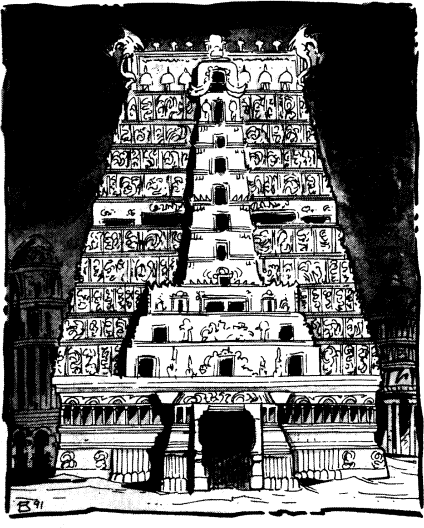
\includegraphics[width=\columnwidth]{images/tyr-1.png}
\par\textit{\small\textcopyright Wizards of the Coast, 2020.}
\end{figure}

\City{Tyr}
{15,000 (70\% humans, 10\% dwarves, 9\% half-giants, 6\% muls, 3\% elves, 1\% half-elves, 1\% other).}
{Iron, silk.}
{Common, Dwarven, Elven, Tyrian.}
{
	Located in a fertile valley in the foothills of the Ringing Mountains, it was the first city-state to successfully revolt against its sorcerer-king. King Kalak ruled Tyr until he fell to a group of heroes led by the gladiator Rikus, the wizard Sadira, and Agis of the noble house of Asticles. With Kalak dead, the High Templar Tithian stepped forward to take his place as king. Tithian received the backing of Rikus and the others, for the templar promised to free all Tyr slaves and institute other sweeping reforms---promises he actually kept. Tithian had his own agenda, of course, which slowly played out over the decade he held the throne.

	The new king created the Council of Advisers and gave members of the most important groups in Tyr a role in the city's government. Councilors were drawn from all ranks of society and worked diligently to pass laws that would strengthen Tyr's newfound freedom. Tithian allowed the Council to operate independently and virtually run the city while he sought the means to become a true sorcerer-king.

	Urik tried to capture Tyr's iron mines less than six months after Kalak's death. The resulting battles made Tyr's leaders realize how necessary a strong military was, and how important it was to resume iron production and get trade and commerce back on an even keel. During his reign, the new king also faced the problem of finding a way to overcome the Dragon's levy, had numerous skirmishes with raiding tribes, and battled angry giants intent on plundering the city. The Council struggled to stay together in the face of secret agendas and conflicting partisan interests. The templar revolt of Free Year 3 shut down the bureaucracy and public works for nearly two months until those who swore new oaths to abandon the old ways and support the tenets of Free Tyr were given more representation in the Council. The artisan strike of Free Year 6 lasted almost four months, and then ended in increased wages for basic services. Agis and the Council handled most of these crises in one way or another, for Tithian was much too busy to get involved in what he considered to be the chores of government.

	Today, in its twelfth year of freedom, Tyr faces new challenges. Agis of Asticles is dead, so his wisdom and honor can no longer guide the Council of Advisers. King Tithian's rule has come to an end. His ambitions led to his downfall, for he is trapped in the Cerulean Storm (though only a few people know of his true fate). The general populace believes that Tithian died fighting to keep Tyr free, thanks to the tales told by Rikus and Sadira. The heroes decided to keep Tithian's current state a secret, fearing that ambitious defilers might try to free him in order to gain power and prestige. Can Tyr's freedom take root in the Tablelands in the wake of these events, or will it be blown away in a devastating Tyr-storm?

	Tyr citizens remain as untroubled by modesty as they were in the days of Kalak. The less a person has to wear in the heat of the day, the better. Most wear loose-fitting cotton tunics gathered at the waist with wide, colorful belts. Others wear loincloths and vests. Light gauze or silks are draped over heads and exposed flesh to protect the skin from the blistering sun. Turbans and other forms of light headgear often finish off a Tyrian's attire.
}
{
	Four months into its twelfth year as a free city, Tyr must deal with the environmental and social conditions left over from the past decade. The Great Earthquake, for example, struck while most of Tyr's beloved heroes and its king were away. It fell to the remaining members of the Council of Advisers to pick up the pieces. Though the rumbling ground made for a terrifying period of time, Tyr escaped the disaster relatively unscathed. There was some structural damage and a small number of deaths, but most of these occurred in the Warrens. The comparatively weak and dilapidated buildings in this part of the city buckled when the quake hit, burying the residents beneath rubble and debris. Ironically, if the quake had struck during Kalak's reign, even less deaths would have occurred. In Kalak's day, the Warrens were mostly unoccupied. It's only since the First Edict freed the slaves that the Warrens have been filled to overflowing with the new crop of free citizens.

	The earthquake caused other damage. Cracks appeared in the city wall, and a whole section of the wall near the Grand Gate collapsed. Minor damage can be seen throughout the rest of the city, but the most noticeable appears on Kalak's Ziggurat. Great cracks riddle one face of the tower, while another face has collapsed into a heap of rubble. The client villages that dot the valley endured the worst of the quake's effects, however. One village was leveled by the quake, and others were pounded by rockslides that cascaded out of the mountains.

	Beyond the death and destruction, the worst aspect for the city is the refugees. Intelligent races and a wide variety of creatures and monsters have fled the mountains, flooding the valley in search of a safe haven. This, in turn, has sent villagers to the city gates, seeking protection from the ravaging hordes.

	What with the Great Earthquake, the periodic aftershocks that visit the city, and the violent Tyr-storms that occasionally sweep the land, the populace has turned into a frightened mob. Not everyone has succumbed to these base fears, of course, but a significant portion has lost control-the Council desperately needs to find a way to calm the people and restore order. A particularly vocal group claims that Kalak has returned to gain vengeance against the city, calling for open worship of the sorcerer-king to appease his wrath. Others have been trying to placate the elemental spirits of earth, hoping that they'll spare Tyr from their ground-shaking anger. Then there are those who seek to take advantage of the misfortune, looting shops, robbing nobles, and generally taking what they want and need by force of arms. These violent mobs are concentrated in the Warrens, but they sometimes range into other parts of the city to sow mayhem and destruction.

	The Council of Advisers has been working overtime to address these problems, though first it had to deal with King Tithian's supposed death. It established the OverCouncil to rule in Tithian's place so that the business of government could continue.

	Second, it increased the size of the City Guard and commanded it to restore order. Things haven't returned to normal yet, but the situation is much better than it was in the days immediately following the Great Earthquake. Various subcommittees have been set up to handle damage control, to see to the fair distribution of water and supplies, and to handle the refugee problem -both those rushing into the valley and those fleeing the villages for the safer environs of the city walls.

	The situations in the other city-states have added to the general nervousness and apprehension hanging over Tyr. While Urik has sealed itself off from the rest of the Tablelands (except for the heavily armed trade caravans that set out and return at random intervals), Gulg and Nibenay have made a few overtures to the Council of Advisers. Both city-states have offered to aid Tyr, claiming that without a sorcerer-king to defend it, the city is vulnerable to all sorts of terrible dangers. The Council, naturally, has thus far graciously refused these offers. Draj and Balic have recently resumed trade with Tyr, but both cities have changed significantly since the reported deaths of their sorcerer-kings. In fact, though Sadira and Rikus assured the Council that the kings had been disposed of by Rajaat, rumors of their return continue to drift in with caravans, adventurers, and refugees. The worst tales come out of Raam, where confusion, madness, and ambition have given rise to anarchy. Tales of nobles being murdered in their homes, of templars being slaughtered in the streets, and of vicious invaders from a hidden city-state controlled by a king named Dregoth have made the Tyr citizens ill at ease and not quite confident that their leaders can protect them.

	Sadira recently convinced a significant portion of the Veiled Alliance to come out of hiding and join Tyr society. These wizards formed a new group in Tyr, called the Preservers. The Preservers were given a place on the Council of Advisers to reflect their new role in Tyr. Sadira, as their leader and as an important member of the Council, was assigned to the OverCouncil. These good wizards are developing plans and guidelines for helping the city in a variety of ways that adhere to their overall morals and code of ethics.
}
{
\begin{figure*}[b!]
\centering
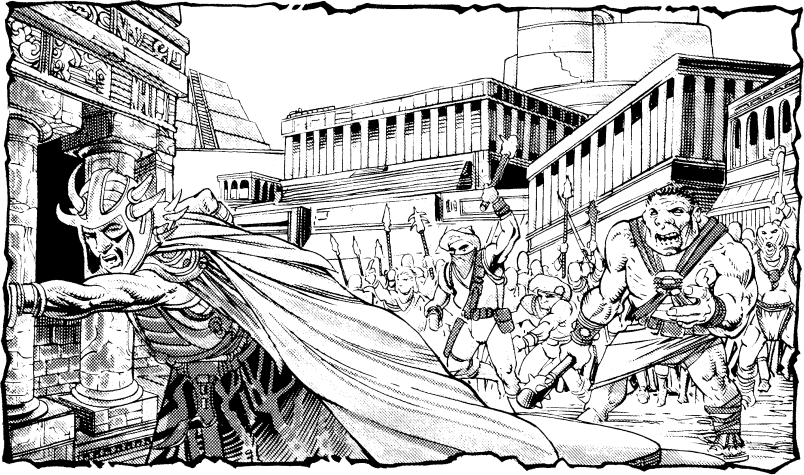
\includegraphics[width=\textwidth]{images/tyr-2.png}
\par\textit{\small\textcopyright Wizards of the Coast, 2020.}
\end{figure*}

	A Council of Advisers makes the laws of Tyr. The Council is divided into five distinct groups who together represent Tyr's varied citizenry. These groups are the Guildsmen, made up mostly of human and dwarf artisans and other professionals from Tyr's three trade districts; the Nobles, representing Tyr's aristocratic families; the Templars, who continue to handle administrative functions in the city; the Free Citizens, chosen from among the masses who were either slaves or paupers before Tyr's liberation; and the Preservers, the newest group admitted to the Council, consisting of members of the once secret and outlawed Veiled Alliance.

	When Rikus, Neeva, and Sadira returned with the news of Agis' and Tithian's death, it was resolved that the Free City shouldn't be burdened with another king. With no king to lead the city, the Council now oversees all aspects of government; a subcommittee made up of one member from each of the Council's divisions serves as an OverCouncil. This OverCouncil governs on a daily basis, while the entire Council of Advisers only meets three out of every fifteen days. The OverCouncil consists of the dwarf stonecutter Gar Bonehammer (NG male dwarf, expert 3) who represents the Guildsmen; Lady Laaj of Mycilen (LE female human, seer 6) for the Nobles; the High Templar Timor (LE male human, defiler 8) for the Templars; Rikus (NG male mul, gladiator 8/arena champion 10) who represents the Free Citizens; and Sadira (N female sun-touched half-elf, preserver 5/veiled one 5) for the Preservers.

	Surprisingly, the Council runs relatively smoothly. Some councilors posture for power and influence and partisan voting sometimes causes meetings to stall, but in general the Council has learned how to get the job done. Each division of the Council meets separately with its constituents to draft its own agenda before coming to a full session. Then the councilors do their best to get their own projects pushed through the voting process while trying to keep in mind the welfare of Tyr as a whole.

	While the Council deals with the big picture, the templars continue to fill the administrative roles they have long been associated with. Since the loss of their spellcasting abilities, it has become doubly important for this division to demonstrate why Tyr needs them. The tangled bureaucracy has been reformed, but it still exists.

	Without the templars to turn the massive wheels of government, Tyr's infrastructure would have collapsed long ago. High Templar Timor (who hides his status as a defiler) serves as the Minister of Tyr, overseeing the various Senior Templars who run departments like Fields, Finance, Public Works, Water, and Trade.
}
{
	\textbf{Free Wizards}: With preserver magic no longer outlawed in Tyr, Sadira convinced a number of preservers to come out of hiding and openly proclaim themselves to the city. As a group the free wizards are not a strong cohesive group. Individual free wizards pursue their own goals, whether in the political arena or merchant activities. Only the desire to instruct the populace in the differences between preserving and defiling magic and to build the public's trust in them unites the group.

	\textbf{House Vordon}: Under the last years of Kalak's reign, House Vordon had fallen from its position as one of the most powerful merchant houses in the Tablelands. Since the fall of Kalak, House Vordon has returned to a position of respect among its peers. The House's return to profitability is fueled by its specialization in the iron trade from the mines of Tyr.

	Thaxos Vordon is head of House Vordon. In the last ruinous days of Kalak's reign, Thaxos began a plan to overthrow the mad king. However, Kalak's demise at the hands of Rikus and the heroes of Tyr stopped him from going forward with the plan. In the years since, Thaxos has become convinced that he should become king of Tyr, and has refined the plan he originally developed for Kalak's overthrow. A number of dummy merchant houses have been created and large numbers of mercenaries hired as part of this plan. Unbeknownst to all but the highest members of House Vordon, Thaxos now has an army scattered at outposts throughout the region, waiting for his orders.

	\textbf{The Veiled Alliance}: The Veiled Alliance remains active in the wake of this new age of wizardly openness. Matthias Morthen (LG male human, preserver 8/veiled one 10) continues to lead a small number of preservers who feel that secrecy must be maintained until all of Kalak's defilers have been eradicated and the citizens of Tyr learn to deal with the responsibilities of freedom. Besides, Morthen doesn't like or trust Sadira, whom he believes has often approached the moral line between defiling and preserving magic (if not actually crossed over it) in the course of defending Tyr. He believes that the Veiled Alliance must continue, if only to serve as a balance for a wizard whose powers and motivations he doesn't fully understand.
}
{
	\textbf{Hidden Village (Thorp, 250)}: Established by the slave tribe known as the Free, the Hidden Village sits in a remote crater in the foothills of the Ringing Mountains between Tyr and Urik. Originally the tribe survived by raiding as most slave tribes do. Now the tribe has advanced into a small trading house. The villagers have developed such a strong relationship with Tyr that they have become a client village of the free city.

	\textbf{Kled (Village, 450)}: Kled is a Dwarven community that has ties to Tyr. Possibly the largest Dwarven community in the Tablelands, Kled was built near the ruins of the city of last Dwarven kings, Kemalok.

	\textbf{Mira's Halo (Thorp, 50)}: Mira's Halo is a merchant outpost owned by House Qual, one of House Vordon's dummy trading houses. The outpost is used in the iron trade between Tyr and Urik. The name of the outpost comes from an unusual rock formation nearby.
}
{
	\textbf{The Elven Market}: The Elven market is located inside the Warrens. Several nomadic Elven tribes trade at the market regularly, bringing a wide range of goods and curiosities from across the Tablelands. Many tribes own a building or two that borders on the square. Others take ownership of unoccupied buildings for the duration of their visit in Tyr. Anything can be found in the Elven market, legal or illegal. The customer just has to know the right people to ask. The market has a reputation for pick pockets and dubious merchandise, but people come from all over the city in order to find items not available anywhere else in Tyr.

	\textbf{Gladiator Stadium}: The Gladiator Arena of Tyr is the second largest building in the city, with only the ziggurat, which looms over one end of the stadium, being larger. The stadium's rectangular floor is some 90 meters long and 24 meters wide. The floor is of a hard packed sand with a reddish hue, which Tyrians say is caused by the spilling of the lifeblood of a thousand fallen gladiators. The stadium is unique in the Tyr Region as it has upper and lower seating sections. The upper section is generally referred to as ``The Sun Seats'' because of the lack of shade, and is open to the general populace. The crowd in the upper section is more raucous and enthusiastic than in the lower section. Seats in the lower section cost more and are traditionally used by merchants, and nobles.

	Despite the end of slavery in Tyr, gladiator matches are still held in the stadium. Now the bouts are not fought to the death and are open to any who wish to participate.

	The gladiator matches are only held on festival days. The remaining time, the arena floor is used for an open air market. A monthly array of tents and stalls cover the sandy floor in drunken rows. Traders who operate in these stalls offer a wide variety of legal and illegal goods and services.

	\textbf{Golden Tower}: The Golden Tower was the imperial home of the King of Tyr. Both King Kalak and King Tithian ruled from the Tower. Constructed of a rare golden granite, the tower gleams harshly during daylight. The only public entrance to the tower is to cross Tower Bridge from the Observation Tower. The public receiving areas are on the top floors, with the King's private chambers on the levels below. These included the King's library, an enormous collection of scrolls and books, many from ancient times.

	\textbf{Iron Mines}: Tyr's iron mines are the largest in the Tablelands and help the city exert leverage over the other cities in the region. The iron mines are located two days, travel northwest of the city. Death has always surrounded the mines, from cave-ins to the ``hej-kin's curse.'' The iron ore is transported to Tyr in heavily guarded caravans.

	\textbf{Kalak's Ziggurat}: The ziggurat built by Kalak still towers over the squalor of the city from its center. The ziggurat is a stepped pyramid with each level finished in a different colored glazed brick. An enormous staircase runs straight from the base to the summit of the ziggurat. Since Kalak's fall, the ziggurat has fallen into disrepair. The Great Earthquake has exacerbated this, causing an entire face of the pyramid to collapse. Great cracks riddle another face of the tower, causing concern that more of the pyramid may crumble soon. Few have dared enter the ziggurat since Kalak's death and it has become the focus of numerous rumors and frightening stories.

	\textbf{School of Thought}: The School of Thought is the only major organized institution for the study of psionics in Tyr. The school was founded a little over 30 years ago by the noblewoman Chessia. Chessia provided the funds to establish the school and made contributions to help the school operate over the years, but she is not involved running the school. The current headmistress of the School of Thought is Sycia Strimmen (NG female human, telepath 7/psiologist 9), a young and enthusiastic woman with considerable charm. She has been the headmistress for almost nine years now, since the previous headmaster, Thanik Arkos, disappeared from the school after murdering one of the master instructors. Sycia is very organized and well liked by students and instructors alike.

	\textbf{Shadow Square}: Shadow Square is a small entertainment district in the Warrens near Kalak's Ziggurat. Five lanes end at the small plaza around which sit six wineshops, a gambling house, and two hostelries. Most business in the square happens between sunset and dawn.

	\textbf{UnderTyr}: The site the city of Tyr was built on has been inhabited for thousands of years. The current city sits atop the ruins of these previous civilizations. An undercity of interconnecting byways, crumbled buildings, and dilapidated courtyards exists under the streets of modern Tyr. From buildings used as businesses to former residences and temples to forgotten gods all make up the structures of UnderTyr. It is not possible to travel from one side of the city to the other through UnderTyr. Instead pockets exist throughout the city. The location of the eight largest pockets is scattered and unconnected across the city. With names such as the Sorrows, Elven River, and Merchant's Maze, these underground locations provide opportunities for the brave or foolish. Many strange and wondrous items can be found in UnderTyr, as can dangerous creatures and malicious entities.

	\textbf{The Warrens}: The Warrens sprawl across the northern quarter of the city. The slum is filled with dilapidated structures and trash dumps. The district is filled to overflowing with the poor, mostly ex-slaves. Many are out of work, and the desperate and ambitious have chosen to prey on their neighbors. Gangs roam the Warrens targeting anyone who looks like they might have a ceramic piece. Templars and the city guard rarely patrol the Warrens anymore for fear of being overrun by the mob. Parts of the Warren are said to be cursed. Other buildings are said to be haunted or the lair of some wild beast. Anyone who enters the Warrens does so at their own peril.
}
{
	\item Slavery is outlawed in Tyr, but a group of slavers has set up a network to kidnap citizens of Tyr and sell them as slaves in other cities. The slaver network is elaborate, involving snatch teams that kidnap the victims, nobles whose estates are used to hold the captives, templars who look the other way, an Elven tribe that smuggles the slaves out of the city, and a merchant house, perhaps House Shom, that transports the captives to other cities where they are sold.
	\item Is the shadow of Kalak's ziggurat deadly? Rumors fly that ever since King Tithian's death, people are suddenly dropping dead while standing in the ziggurat's shadow. Those living close to the ziggurat are fearful of falling under what they have named Kalak's Curse. Many are fleeing, but no one knows what is causing the deaths.
	\item The elderly noblewoman Prisella Obstrunia is unlike many of her fellow nobles. Since the slaves were granted their freedom she has come to regret her past participation in the practice, and seeks to make amends somehow as she nears the end of her life. One of her former slaves, Raxenth, has remained with her as a servant and become a friend. When slavery was still in practice in Tyr, Prisella had sold off a number of Raxenth's relatives. Now, she wants to reunite Raxenth with these relatives, who through the slave trade have been scattered across the Tablelands. The noblewoman will hire the PCs to track down Raxenth's relatives and bring them back to Tyr.
	\item Zacraloc is the landlord for a large section of the Warrens, where most of the poor cannot afford to own their own homes but rent dilapidated buildings from Zacraloc. Seeking to increase his land holdings, Zacraloc uses hired thugs to set fire to a large section of the Warrens, which he does not own. His intentions are to approach the owners of those who lose their houses in the fire and offer to buy the ruined homes for very little money, since the desperate victims will need any money they can get. But the fire spreads out of control fed by either fire clerics or fire elemental creatures attracted to the original blaze.
	\item One of the rare, well-respected templars with no known enemies is found murdered. The templars are demanding better protection and seek to use the murder for political concessions by blaming the freemen. Freemen politicians reject the acquisitions but attempt to hinder the investigation, because they fear what would happen if the allegations were true. The truth is that it was not a political murder. The templar was murdered by a woman he sold into slavery years ago to merchants from Balic. The woman only recently escaped slavery during the confusion of the Wavir coup and returned to Tyr where she tracked down the person responsible for her enslavement.
	\item Tired of the raids by hej-kin on the iron mines, the Council of Advisors decides to send emissaries to the hej- kin to negotiate some sort of truce. Timor, the senior templar on the Council, does not believe the negotiations will be successful so before the PCs leave he secretly asks them to map out their journey to the hej-kin lair. With this map, a military expedition can be led to wipe out the hej- kin threat. To further complicate the PCs' mission, an agent of King Hamanu has infiltrated the mine as a guard and seeks to broker an agreement with the hej-kin on behalf of his master.
}
\begin{figure}[b!]
\centering
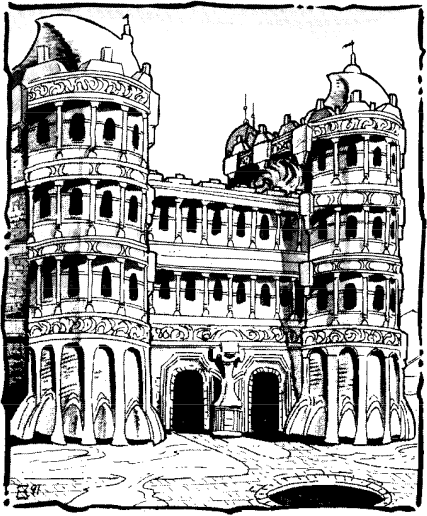
\includegraphics[width=\columnwidth]{images/urik-1.png}
\WOTC
\end{figure}

\City{Urik}
{30,000 (75\% humans, 10\% half-giants, 5\% dwarves, 3\% muls, 3\% thri-kreen, 2\% elves, 1\% halfling, 1\% other).}
{Obsidian, silk, pottery.}
{Common, Dwarven, Urikite.}
{
	Located northeast of Tyr, between the Dragon's Bowl and the Smoking Crown Mountains, the square, clean lines of the city-state of Urik can be found. The city-state has remained virtually the same as it was before the Great Earthquake and the demise of the Dragon. Hamanu, the King of the World and the Lion of Urik, was away from his city when the tremor struck.

	Although minor damage and only a few deaths resulted from the quake, the citizens trembled. When Hamanu returned, he promised his citizens that they would have nothing else to fear from Athas and its cruel temperament. The sorcerer-king's word (and his magic) was as strong as precious steel, for neither the aftershocks nor the Tyr-storm that arrived two months later could breach the towering yellow walls of Urik.

	Hamanu's promise wasn't unconditional. Though the Urikites don't have to fear change, they do have to fear their king. To disobey Hamanu is to risk punishment and even death, while to obey him is to live without fear. That's how it's always been in eternal Urik, and that's how it always will be.

	Urikites wear their hair in square cuts with elaborate ringlets. Some men wear square-cut curled beards. White linen shirts with short, tight sleeves are the fashion of Urik. Individuals of the lower classes wear plain, unadorned shirts that fall to their knees. Individuals of the upper classes increase the length to their ankles and add a striped or diamond pattern as well as a tassel-trimmed girdle. Elaborate scarves, worn only at night, indicate a citizen's station. The longer and richer the scarf, the higher the wearer's social status. By law and tradition, only templars may wear cloaks, and these are always bleached pure white for the low to mid levels and tinged yellow for the higher ranks.
}
{
	Except for the new restrictions regarding trade and travel, things in Urik are the same as they ever were. The city remains a warrior culture, ruled by a warrior king and geared toward fighting and winning wars. The current enemies aren't the other city-states, however. Rather, the refugees seeking shelter from the constant tremors and the monsters fleeing from the violent storms near the Silt Sea have become Urik's foes. When either approaches Urik's high, yellow walls, Hamanu leads his army out of his gigantic palace (called Destiny's Kingdom) and charges into battle. In most cases, the result is slaughter, for terrified invaders can't stand against Hamanu's highly trained and well-equipped legions.

	The few signs that the Great Earthquake touched Urik have been wiped out; buildings have been repaired, streets repaved, the dead buried. Now, Hamanu's magic keeps the aftershocks and the storms from entering the city, and in most respects the citizens have learned to ignore the disasters. As long as the disasters remain outside Urik's walls, the citizens see no reason to worry about them.

	Closing the city off from the rest of the world has made it difficult for certain members of Urik's society. Adventurers and traders, for example, are severely hampered by the well-guarded walls. Elves, never really welcome near Urik's walls, now avoid the city completely. They are treated like invaders, set upon as soon as they're spotted entering Urik's verdant belt. Things may change as soon as the king finishes contemplating his city's new approach to the world---or it may simply get worse if Hamanu decides to keep the rest of Athas at bay forever.
}
{
\begin{figure*}[b!]
\centering
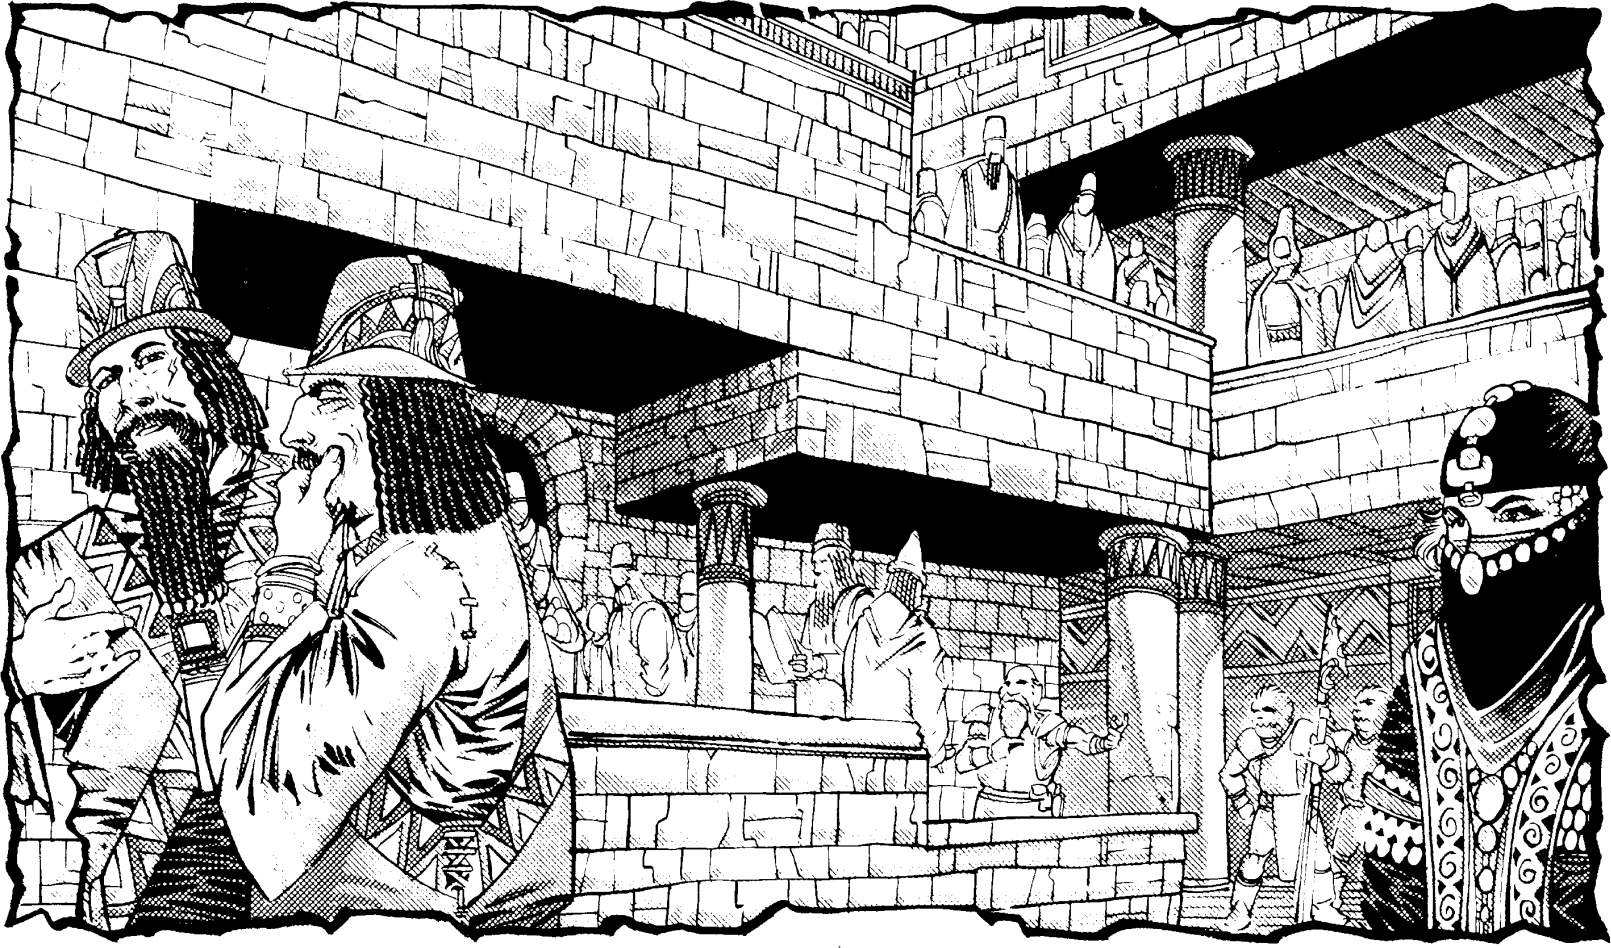
\includegraphics[width=\textwidth]{images/urik-2.png}
\WOTC
\end{figure*}

	The sorcerer-king Hamanu rules Urik, taking a personal interest in the affairs of his city. Except for Hamanu's direct involvement, Urik operates as a traditional sorcerer-king's domain. Templars enforce Hamanu's laws and handle the day-to-day bureaucracy, nobles manage the farms and water supplies, free citizens engage in business and try to remain free, and slaves provide the muscle to get everything else done.

	Hamanu is a third-stage dragon king (LE male Champion of Rajaat stage III dragon, defiler 5/psychic warrior 11/arch defiler 10/cerebremancer 5/Athasian dragon 4). Through a combination of the Way and magic, he appears before his subjects as either a tall, vigorous man with close-cropped silver hair, dark skin stretched tight over ruthless features, and heartless yellow eyes, or as a half-man and half-lion of powerful build and mythic proportions. He is never seen in his true dragon form, even by his most-trusted templars. His laws, called Hamanu's Code, are strict and innumerable, covering almost every conceivable aspect of life in Urik. Hamanu's Code relies on punishment in kind and emphasizes loyalty to the king and his templars. The Code stands unsurpassed in the Tyr Region for utility, comprehensiveness, and ruthlessness.

	At one time, Hamanu's ambitions exceeded his resources. Since the Great Earthquake and the events surrounding Rajaat's brief return, his agenda has subtly changed. The three surviving sorcerer-kings sensed that the time had come to rethink the old ways, to find new approaches to the challenges of life on Athas. Until he figures out what those new approaches are, Hamanu has decided to withdraw a bit. He has effectively closed Urik off from the rest of the Tablelands, trying to keep change from intruding on his domain for as long as possible.
}
{
	\textbf{The Brotherhood of the Mind}: The Brotherhood of the Mind is an organization of evil psionic-users that wish to overthrow the sorcerer-kings and seize power for themselves. Ruled by Liumakh, an undead psion, (NE male undead, telepath 10/thrallherd 7) the Brotherhood is headquartered in a monastery in the Smoking Crown mountains. Both Hamanu and Nibenay know of the brotherhood's existence. Nibenay seeks their destruction, while Hamanu ignores them for the most part, though he occasionally spies on the brotherhood to see if they have developed anything interesting during their psionic studies.

	\textbf{Hamanu's Halflings}: Hamanu has forged an agreement with a halfling chief from the Ringing Mountains. As long as Hamanu provides the chief with obsidian from the Urikite mines, he receives the services of 200 halfling warriors. These halflings are excellent night raiders and assassins that Hamanu has used to deadly effect in the past.

	\textbf{House Stel}: House Stel is best known for trading in the spoils of war, weapons, slaves, and various stolen cargo. Heavily influenced by the militant nature of Hamanu's regime in Urik, Stel is aggressive and confrontational with rivals. Stel caravans are heavily guarded to prevent against raids from other merchant houses, a tactic the house uses on its rivals regularly. The leaders of House Stel have a deep hatred of elves which has led to open warfare with a number of Elven tribes over the years. The House maintains lucrative trading contacts with halflings of the Ringing Mountains. Hargan Stel III (LN male human, fighter 5/rogue 2/ dune trader 5) leads the house and reflects the nature of his house, being both an expert trader and warrior.

	\textbf{The Veiled Alliance}: The Veiled Alliance has to be doubly careful in the wake of Hamanu's restrictions, and the preservers' supplies of spell components have become extremely limited. For most of the decade following the war with Tyr, Urik's Veiled Alliance was split into two factions. Its leader, the legendary Morlak, disappeared mysteriously, leaving two preservers to contend for the spot he vacated.

	When one of the contenders, Leoricius the Untamable, was killed in the Great Earthquake, the other contender worked feverishly to heal the split. This became increasingly important in the wake of Hamanu's newest restrictions. Today, Thania (LN female half-elf, preserver 5/veiled one 7) commands a whole Alliance, advocating patience and negotiation instead of the violent confrontations advocated by her one-time rival. Thania has been working to establish a partnership with Tyr's Alliance, but if Hamanu learns of it both groups will undoubtedly suffer.
}
{
	\textbf{Makla (Village, 1,000)}: The obsidian mines of Urik are located on the Mountain of the Black Crown, a peak in the Smoking Crown mountain chain. Urik's economy is completely dependent on obsidian and the tools fashioned from it. The Urikite client village of Makla serves as a base camp for the mining operations on Black Crown. The village is located on the shores of the Lake of Golden Dreams. Heavily fortified with over 500 guards, it is rarely attacked by raiders.

	\textbf{Fort Courage}: Fort Courage is a massive fortress on the trade road between Makla and Urik. This facility of House Stel is a supply point for caravans traveling between Urik and Makla and the halfling village of Ogo. Patrols are also sent from the fort to discourage raids on caravans along this route.
}
{
	\textbf{Destiny's Kingdom}: Sorcerer-King Hamanu rules Urik from his palace inside the massive fortress of Destiny's Kingdom. The walled fortress covers one square mile at the center of the city, containing troop barracks, drill fields, and an armory to support the army, as well as administrative offices for the king's templars.

	\textbf{The King's Academy}: The only legal psionic school in Urik is located within Destiny's Kingdom and is called the King's Academy. Students who attend the Academy are subject to a strict education that brings harsh punishment for failure. At the same time students are indoctrinated with the militarism that runs through the government of Urik.

	\textbf{Little Jungle}: A portion of the drill fields inside Destiny's Kingdom has been set aside for Hamanu's halfling allies to make their homes. Little Jungle is the name given to the fenced off area, where the halflings build huts in the jungle style.

	\textbf{Pit of Black Death}: Urik uses the site of an old obsidian mine for a gladiator arena, thus giving the arena its name, the Pit of Black Death. The Pit does not rise above the ground but is sunken into the ground. Stepped excavation provides viewing platforms for the crowd. All spectators must stand in the Pit, as there are no seats in the arena. The irregularly shaped combat area is made entirely of obsidian. The sun heats the black obsidian until it becomes almost unbearable for both combatants and spectators. As such most gladiator matches are held in the morning before the heat has become too great, or on rare occasions at night. Another danger of the obsidian is the thousands of sharp edges, shards, and spikes that protrude from the walls of the arena. These obsidian shards cover the walls and columns of obsidian that are scattered around the arena floor.

	\textbf{Potter's Court}: Pottery is an art form in Urik, and all other city-states recognize the superiority of Urikite pottery. The potters' workshops are collected in the Potter's Court area of the city. The concentration of so many immense kilns in the area, make Potter's Court unbearably warm, even at night when most of the potters conduct their work.

	\textbf{Potters' School}: The Potters' School is the largest group of psionic users who refuse to attend the King's Academy or register with the authorities. While the Potters' School teaches pottery casting and painting, skilled psions instruct students in the Way, outside of the influence of King Hamanu and his templars. The head instructor of the psions is Erriok (LN male human, shaper 7). He is rumored to have contact with the Veiled Alliance and work with them on occasion.

	\textbf{Three Sisters Observatory}: The Three Sisters Observatory is a two storey building with a flat roof and many observation balconies built on top of a hill called Sunrise Point. The Three Sisters Observatory served as the king's observatory until the construction of the Royal Observatory. Now the building is used to store old astronomical records and equipment, and has a run down, neglected appearance. The observatory gets its name from three identical granite hills nearby.
}
{
	\item Templars arrive at where the PCs are staying with orders to arrest them. Someone has accused the PCs of practicing magic. A fair trial is not possible and the sentence is death. The PCs must escape the templars, find out who their accuser is, and clear their name before they are captured by the templars.
	\item Unbeknownst to the PCs, their names have been added to a bounty list the templars of Urik maintain. Templars and bounty hunters begin to appear, trying to collect the bounty by capturing or killing the PCs. Whether or not the PCs are wanted by the templars, in this instance it is a case of mistaken identity. A wealthy merchant, wanted for smuggling, is supposed to be on the bounty list, however, he bribed a templar to remove his name and that of his family from the list. The PCs' names were chosen at random and added in place of the merchant's and his family to fill the vacancy.
	\item House Wavir has heard rumors that King Hamanu is planning on ordering his templars to seize all of their house's assets in Urik. Using the Wavir coup in Balic as an example, the house will be accused of planning a rebellion in Urik. Before he goes through with this threat, Hamanu is checking with the other major merchant-houses to gain their acceptance of his actions so they do not boycott his city. House Wavir gets wind of the plot and secretly plans to sneak out of the city with as much of their assets as possible. The PCs are hired to coordinate and have to safely get the Wavir agents and as much of their various assets, including wagons, merchandise, and draft animals, out of the city.
	\item The PCs are attending a feast at a noble's compound when the head of the family is murdered. Templars descend on the compound preventing anyone from leaving. Instead of investigating the crime, the templars simply state that unless the murderer is presented to them by morning everyone in the house will be executed. The PCs have until morning to find the real killer, or be executed along with everyone else.
	\item The Veiled Alliance has wondered for years about the high drik transformation process. The PCs are assigned to steal a drik egg that has undergone the process but that has not yet hatched.
	\item Saita, a templar of Urik, secretly sold some of the city's slaves to a tribe of yuan-ti in the Ringing Mountains to make some extra money. Unfortunately, the slaves were the personal property of Hamanu who is now enraged that his slaves are missing, and wants the head of the person responsible. Saita is desperate to get the slaves back before it is discovered that she is the one responsible. She secretly hires the PCs to get the slaves back from the yuan-ti any way they can.
}
\section{Beyond the Tablelands}
Plenty of action and adventure can be found across Athas. More lands of wonder, mystery, and danger exist beyond the barrenness of the Tablelands. A quick tour of these other places follows, and more information about specific locations will be revealed in future products.

\SubCity{Eldaarich}
{21,000 (85\% humans, 8\% dwarves, 4\% half-giants, 2\% muls, 1\% others).}
{Gold, silver.}
{Eldaarish, picts.}
{
\Figure*[\textwidth-2cm]{b}{images/city-eldaarich-1.png}

	Eldaarich occupies a small island in the Sea of Silt, just off the mainland. Here, isolated and protected from the rest of Athas, the citizens huddle in the paranoid delusions of their mad sorcerer-king. Daskinor, ruler of Eldaarich, believes that unknowable forces in the world are trying to destroy him.

	Every few years he puts a new name to these forces---the Order, the Veiled Alliance, Rajaat, pyreen, a merchant house, a lowly slave, or some other identifiable target becomes the imagined source of his fears for a time. Daskinor does his best to destroy these imagined enemies, and anyone who has even a passing resemblance to the target is persecuted until the next delusion grips him.

	Daskinor was never a stable ruler. From the beginning of his reign as sorcerer-king of Eldaarich, he was tormented by unfounded fears and nameless terrors that preyed upon his mind. For the first few centuries of his reign, he was able to function more or less normally despite his growing paranoia. As time passed, genuine bouts of panic began to intrude upon his psyche. These bouts lasted longer and longer, paralyzing Daskinor for hours, days, sometimes even months at a time.

	Eldaarich was constructed to protect Daskinor from his fears. Fortified walls, a strong military, devoted templars, retractable bridges, and a series of keeps and forts ensured that the entire city-state and surrounding area was secured against outsiders. Over time, it became less of a fort and more of a prison, locking king and citizens alike behind sturdy gates and high walls. Seven centuries ago, the sorcerer-king's paranoia became acute. He completely sealed his city, cutting off all ties to the other city-states. That was the way things remained until about FY 0 year, when limited trade was resumed with House Azeth of Kurn.

	Today, Eldaarich remains an isolated prison of a city. Daskinor's fears have become the fears of his citizenry, making everyone who lives under his rule as paranoid as he is. No one ever leaves Eldaarich, and no one ever enters its massive gates. It's a closed society---figuratively and literally.
}
{
	Every outsider wants to destroy their city-state and their sorcerer-king, and everyone who lives within the walls waits for an opportunity to betray you. That's what the people of Eldaarich believe, for that's what their leaders believe. Nowhere else in all of Athas is there such an underlying current of genuine, unattributable fear. It filters down from Daskinor himself, making citizen and slave alike tremble with uncontrollable paranoia.

	The citizenry is a subdued, cowering lot, given to unexpected bursts of violence once the fear inside them becomes too much to contain. In many cases, the ever-crushing weight of terror and oppression keeps the masses down, but sometimes a delusional artisan will strike out at a templar or noble, causing the level of paranoia to rise even higher.

	The quality of life isn't good in Eldaarich. Because Daskinor doesn't trust anyone, he allows his templars to dispense only the barest essentials to the free citizens and slaves. With just enough food and water to sustain them and few personal possessions, the people of the city are a sad, pathetic lot. They have no hope of a better life and no concept that a better life exists outside the walls of Eldaarich. If anyone even suggests such a notion, the ingrained fear of the unknown kicks in and makes everyone else dismiss the idea.

	While the class structure of noble, free citizen and slave exists in Eldaarich, the truth is that everyone beneath the templars is a slave to Daskinor's all-pervasive fear.

	The sorcerer-king sees threats to his rule on every face and in every dark shadow. For this reason, he permits no freedoms of any sort, not even the token rights given to the citizens of other cities. Freedom, Daskinor believes, is just an opportunity to betray his trust. So he orders his templars to oppress the people of his city, to make their lives so miserable they don't have time or strength to contemplate treachery.

	The templars don't have it much better. They're kept in line by the high templars who, in turn, are subject to Daskinor's brutal whims.

	The majority of the population consists of humans, though there are also dwarves, half-giants, and muls in significant numbers. There are also a few aarakocra wasting away in the slave pens. Daskinor has a particular hatred of the winged people and gives his templars special compensations for capturing aarakocra from the nearby White Mountains.

	If travelers were to find themselves in Eldaarich or one of its holdings (which isn't very likely), they'd feel the weight of oppression and smell the stench of mental illness that hangs in the hot, stifling air. Every year the darkness in Daskinor's soul grows deeper, his paranoia more acute. This mental deterioration is reflected in the city itself, as though each citizen were a part of the sorcerer-king's diseased mind.
}
{
	The same model of government evident in the other city-states exists in Eldaarich. The sorcerer-king Daskinor (CE male stage II Champion of Rajaat dragon defiler 8/nomad 10/cerebremancer 10/Athasian dragon 2) stands atop the societal hierarchy, his troubled delusions coloring every aspect of life in the city-state. His chaotic tendencies and often overwhelming paranoia infuse everyone he comes in contact with, making the city almost as wild and frenzied as Raam. The only thing that allows the city to function is that the citizens are a subdued lot, living in quiet fear instead of in rambunctious anarchy. Daskinor constantly watches over his shoulder for assassins that don't exist, and so do his templars and nobles. No one trusts anyone else in Eldaarich. This works out for the best, as the troubled atmosphere has fostered a society where the fear of murder and betrayal has encouraged the periodic use of such techniques by those who prefer to strike first.

	Templars and nobles regularly kill each other to keep the same from happening to them, or to gain power or position, or just because the tension of living behind heavy locks and being constantly on guard eventually drives even the most peaceful beings to violence. In Eldaarich, fears permeates everything---fear of the sorcerer-king, fear of outsiders, fear of each other, and fear of the unknown. Because the society is closed off to the rest of the world, everything on the other side of its walls and locked gates is, by definition, unknown.

	If Eldaarich is a prison, Daskinor is its most prominent prisoner. The sorcerer-king lives in a walled sub-city and rarely ventures into other parts of his realm. His constant paranoia sometimes intensifies to such a fevered pitch that he ceases to function.

	In such a state, which may last as long as months at a time, Daskinor is cared for by his senior templars. At other times, his paranoia drives him to give a name to his fear. When this occurs, the entire city mobilizes to combat this supposed threat to the realm. Currently, the use of psionic abilities has been outlawed, as Daskinor believes that the Order has initiated a campaign against his rule. Even low-powered psionicists and wild talents who openly display their abilities are subject to imprisonment or death because of the current edict. Only Daskinor, a psionicist of the highest caliber, is exempt from the terms of the edict.

	Daskinor's templars serve as administrators to the city, and also act as the sorcerer-king's eyes and ears in all corners of the domain. They are charged with watching for signs of treachery among the masses-and with dealing with such treachery before it gets out of hand. The templars are as paranoid and delusional as Daskinor, giving in to their fear whenever it overwhelms them. For this reason, Eldaarich has become a police state, and the templars are the police. They command the military. They oversee all records and the distribution of goods and services. They hold the power of life and death for the rest of the citizenry in their terrified hands.
}
{
	\textbf{Kulag:} The Kulag Order controls Daskinor's silt fleet, which currently acts as the merchant house for the Dim Lands, a nearby archipelago. It is leaded by High Templar Kerillis (LE female human, templar 14). Sometimes they also resort to piracy in the nearby islands.

	\textbf{Neshtap:} More commonly known as ``red guards'', the Neshtap are the most feared, and the second-most powerful of seven orders that Daskinor uses to maintain control of his city Eldaarich, and its client villages. They never speak, seemingly revere the element of fire, and are becoming increasingly powerful and independent from Daskinor.

	\textbf{The Veiled Alliance:} Eldaarich has no Veiled Alliance. Daskinor rooted out the Alliance and destroyed it 400 years ago when the group of preservers became his imagined enemy of the moment. Some preservers still live in the city, but they remain hidden and are relatively weak due to a lack of adequate training. Preservers from Kurn sometimes sneak into the closed city to provide training and to see what the conditions are, but they don't do this very often. If they get caught, they're put to death, and if their city of origin is discovered, it could mean war between the two cities. No one, especially Oronis the Avangion of Kurn, wants a war to break out. He does, however, feel the pain that both Daskinor and his citizens project, and often contemplates finding a solution to Eldaarich's problems.
}
{}{}
{
	\item A silt schooner owned by House M'ke was attacked and captured by the navy of Eldaarich. The merchant house could hire the PCs to raid the harbor of Eldaarich and bring the schooner back.
	\item An aarakocra from Winter Nest was captured when she flew too close to Eldaarich. The PCs are asked to free her before she is executed by the templars of Eldaarich. Once freed from her cage, the aarakocra can easily fly back to Winter Nest on her own, but the PCs will have to sneak out of Eldaarich.
	\item Grehgatha is a Kurnan preserver who has snuck into Eldaarich many times to tutor young preservers. Since she has returned from her last attempt she is consumed with freeing an entire village from Daskinor and hires the PCs to help. The PCs must come up with a way to sneak 150 people past the templars of Eldaarich.
	\item The Red Guard has become jealous of the monopoly on trade held by the templars of the Kulag Order. In an attempt to disrupt the trade negotiations, the Red Guard mounts a surprise attack on Silt Side during a meeting between Corik Azeth and High Templar Kerillis. The PCs acting as guards for House Azeth may misinterpret the attack as directed by Corik or themselves.
	\item Concerned with a recent rise in the level of the silt sea around Eldaarich, the city has declared war on all silt clerics. Mercenaries are to be hired to help hunt down the silt clerics along the coast for a hundred miles north and south of Eldaarich. The PCs could become embroiled on either side.
	\item A major giant raid on the Huuros Islands has been repulsed by the Kulag Fleet, though many casualties were suffered. Templars assign the PCs to salvage what they can from the battle, equipment as well as the bodies of those who died. Most of the wreckage is just off shore in silt 4.5 to 6 meters deep.
}


\SubCity{Kurn}
{18.000 (65\% humans, 10\% elves, 6\% muls, 6\% aarakocra, 5\% dwarves, 4\% half-elves, 3\% half-giants, 1\% other).}
{livestock, magic items, medicines.}
{Elven, Kurnan.}
{
\Figure*[\textwidth-2cm]{b}{images/kurn-1.png}
	Kurn is actually two city-states: an ancient, public metropolis, and a utopian city hidden from the rest of the world. Old Kurn sits in a lush meadow on the eastern side of the White Mountains. The trade road running north out of Draj connects Kurn to the Tyr Region, and the city welcomes merchants from the south. New Kurn lies in a fertile valley hidden among the White Mountains themselves. A secluded road protected by a towering fortress keeps the valley safe from unwanted visitors---and New Kurn doesn't want any visitors.

	Old Kurn was a prosperous but relatively small city from the Green Age that suffered great devastation in the early days of the Cleansing Wars. Once situated in a vast forest that has long since faded from the landscape, the elf city of Kurn was destroyed by the Champion called Albeorn, Slayer of Elves. When the Champions finally turned against Rajaat and became the dragon kings, the one named Keltis decided to build his city-state on the ruins of Old Kurn. He changed his name to Oronis, but decided to retain the name of the city he was building over.

	The ruins weren't in as bad a shape as Oronis originally thought. He was able to build upon many of the foundations, and a few whole structures were still fit for use. Within a decade, Oronis' Kurn was established. Within five decades, it was thriving. For five hundred years, Kurn followed the same course as the other sorcerer-king domains. Throughout that time, Oronis was troubled by something few of his peers possessed---his conscience.

	When he was Keltis, Lizard Man Executioner, he succeeded at the task Rajaat handed to him. He eliminated the entire race from the face of Athas. As the years passed and Keltis the Champion became Oronis the sorcerer-king, images of the atrocities he committed started to haunt him. After Oronis advanced to a second stage dragon king, his problems intensified. Now he had the deaths of his subjects on his head, for he had to use a specified amount of life force to power his transformation.

	He decided that none of this was what Rajaat originally promised him. Where was the restoration of the world? Athas hadn't gotten better because of the Cleansing Wars. It had gotten worse. What's more, the sorcerer-kings were continuing the downward spiral, slowly killing the world by their actions. Oronis refused to be a part of that trend any longer. He renounced his defiling skills and his status as a dragon king and sought a different path.

	That was when Kurn broke off relations with the other city-states. Mercantile activities continued, of course, but at a reduced rate. After a time, Kurn became one of the forgotten cities---just as Oronis had hoped. In the meantime, he set the next part of his plan for redemption in motion. Oronis wanted to make amends for the horrors of his past.

	The first step was to change the rules of society in Kurn. Though the city had to maintain an illusion of normalcy to keep the other sorcerer-kings from detecting treachery or weakness, Oronis secretly freed all slaves and instituted fair and just practices at all levels of society. He swore his citizens to secrecy, for if word got out he was sure his one-time peers would flock to Kurn like gith to a dying braxat. The second step was to begin construction on the utopia he envisioned. Like all ex-Champions, Oronis originally wanted to return Athas to the glory of the Blue Age.

	He decided to once more strive for that goal. In a hidden valley among the peaks of the White Mountains, the foundation stones of New Kurn were laid. As his templars and citizens worked to build New Kurn, Oronis went in search of a better path to power. Using the techniques and practices of preserving magic, Oronis looked for a way to combine magic with psionics in a more positive way than through dragon magic. It took nearly 1,000 years of study and experimentation for Oronis to develop the preserver metamorphosis spell. With it, the reformed sorcerer-king could become an advanced being aligned to goodness instead of another force for evil.

	Today, the twin cities of Kurn continue along their parallel courses. Old Kurn displays a typical sorcerer-king's domain to the other inhabitants of the region, at least on the surface, while New Kurn works to complete Oronis' experiment in regressing a small portion of Athas back through time. Between the two cities, Kurn has a total population of 18,000 people. The majority live in the new city, as each year more citizens are moved from the old city to the new. Old Kurn has such a small number of residents that it appears to be almost a ghost town, and one day Oronis plans to completely abandon it in favor of his secluded valley.
}
{
	The state of life in Kurn depends on which of the twin cities is being considered. Old Kurn, on the surface, appears to be much like any city in the Tyr Region still ruled by a sorcerer-king. Surface appearances, however, can be deceiving. Travelers who stay for any length of time might notice a few oddities. For example, the slaves seem to have a sparkle in their eyes and a bounce in their step that isn't seen in the other city-states, and templars aren't given as wide a berth as their counterparts in Urik or Nibenay. Additionally, while the merchant and tradesmen districts are always crowded, the rest of the city is as empty and desolate as the ruins of Giustenal.

	Old Kurn maintains its illusion of business-as-usual through the cooperation of its citizens and the advanced powers of its sorcerer-king. If visitors notice that the noble and templar quarters of the city are practically deserted, they usually attribute it to the rumors that Kurn is slowly dying. Dying or not, the city is far from defenseless. More than one raiding tribe has attempted to take advantage of the ``dying'' city only to discover that its defenders were more than capable of driving them off.

	Through the efforts of House Azeth and the commerce provided by other traders, Kurn maintains a modest economy. While most of the inhabitants of the Tyr Region have forgotten that this northern city exists, Kurn interacts with its closest neighbors on a regular basis. It has good relations with the aarakocra of Winter Nest, the merchants of Draj's House Tsalaxa, and the elves of a few of the local tribes. Except for the contact between House Azeth and the trade templars of Eldaarich, Kurn has little interaction with its neighboring city-state. On the other hand, Kurn sometimes has trouble with raiders from the Bandit States. The raiders don't come to the gates of the city (at least not very often), but they do attack travelers on the trade road and even plunder the client villages on rare occasions.

	New Kurn is a different matter. The high, sturdy walls of Fort Protector block the eastern entrance to the hidden valley, while the tall, steep peaks of the White Mountains make the other directions inaccessible. The only approach that might be open is by air, though flying creatures loyal to Oronis nest in the vertical peaks.

	Within the valley, Oronis' restoration project is in full swing. He has turned the valley into a place from the past, recreating the conditions of the Green Age in its sheltered space. A thick forest surrounds a lush clearing where the city of New Kurn has been built beside a small, clean lake. Oronis hopes to eventually regress the valley to conditions as they were in the Blue Age, but that's still many years away.

	The new city resembles Oronis' vision of utopia. Airy buildings with tall, elegant spires grace wide, open streets paved with white stone. Here, the people govern themselves through a system of fair laws and majority rule. Everyone has a say in the workings of the city, from the poorest laborer to the highest elected official. And if someone doesn't like the way things are going, they're free to run for a position when the current terms of office expire.

	Thanks to the fertile valley and the lush forest, no one goes hungry or thirsty in New Kurn. No creatures are hunted out of existence and no plants are plucked completely from a given area. The templars monitor the forest on a daily basis to make sure the delicate balance is maintained. For this reason, no defilers are permitted within the ranks of the templars or anywhere in the twin cities. It is strictly against the laws of Kurn to practice defiling magic.

	Oronis continues to advance as an avangion, and he tries to instill the same serene, peaceful, life-giving properties of his new form in the city and people who follow him. Where once there was a man of evil, now Oronis is a force for good in the world. His templars work to promote his plans and prepare to someday strike out from the valley with the knowledge of how to restore all of Athas. Until then, they'll work to finish the restoration of the valley and to perfect the society that Oronis has inspired.
}
{
	Oronis the Avangion (LG male Champion of Rajaat stage IV avangion, preserver 5/shaper 5/cerebremancer 10/loremaster 3/avangion 5) guides the paths of the twin cities. Oronis spent centuries redeeming himself, going so far as to change his very nature from evil to good, though he still feels he has a long way to go to make up for his acts as a Champion of Rajaat and a sorcerer-king. For this reason, he has dedicated himself and his citizens to working toward the eventual restoration of all Athas.

	While in Old Kurn, Oronis wears the guise of a normal human. In this psionically and magically induced disguise, he appears as a tall, lanky, middle-aged man with short golden hair, pale-blue eyes, and a close-cropped blond beard. He covers himself in the trappings of a sorcerer-king, wearing a golden circlet on the crown of his head and carrying an obsidian-topped walking staff. In New Kurn, however, such disguises aren't called for. There he openly displays his true avangion form---a tall, thin, hairless humanoid with golden skin, silver eyes, and gossamer wings.

	Though Old Kurn appears to run like any other city-state, Oronis long ago abandoned a monarchical form of government. He allows his subjects to govern themselves via a democratic system he developed. In this system, nobles and all citizens except templars may hold public office. Elections are held at regular intervals and term limits are set. The highest elected official is called the Presider, who sits at the head of a body called the Tribunal. Members of the Tribunal are referred to as Tribunes. Together, the Presider and the Tribunes draft the laws that keep the city-state running smoothly. The current Presider is Ulali of Prusicles (LG female half-elf, preserver 8), now in the second year of a five-year term.

	Oronis refuses to hold an official position, though he does pretend to be sorcerer-king in the old city. He acts as an adviser when the Presider or Tribunal requests his presence, but otherwise, he's more concerned with advancing as an avangion and keeping the valley restoration project on track. Oronis' templars don't serve as administrators in Kurn, either. Instead, they are the keepers and dispensers of knowledge, serving as teachers and advisers to local officials and businesses. It's also their job to oversee and handle the restoration process, under Oronis' supervision.
}
{
	\textbf{Black Brethren:} Oronis' Black Brethren are Kurn's elite army, charged with patrolling Kurn and making sure Kurn is safe and secret.

	\textbf{School of Spies:} Kurn's School of Spies is an organization of Kurnan spies, mostly female, that studies non-Kurnan societies, and brings back information to defend Kurn and improve its way of life. They have managed to infiltrate into Merchant Houses and even the templarate of every city-state in the Tablelands.

	\textbf{The Veiled Alliance:} Kurn has no Veiled Alliance. Preservers are a welcome and significant part of the society, so there's no reason for them to hide behind a veil of secrecy. In fact, preservers from other Alliance factions sometimes come to Kurn to study with Oronis. One preserver, Korgunard of Urik, even learned the steps to become an avangion and followed the path forged by Oronis. It's conceivable that more avangions will appear in the future, though when and how many is hard to say. While preservers are accepted and integral to Kurn society, defilers are considered enemies of everything Oronis stands for. The avangion is reluctant to allow his followers to make defiling magic punishable by death, as he himself was once a defiler of the highest order. However, he knows that in most cases defilers can't make the mental and spiritual changes necessary to reject that path, so he has agreed that known defilers must be banished from the society.
}
{
	\textbf{Azeth's Rest (Village, 900):} This fortified oasis and trade village lies on the trade road, reaching north from Draj to Kurn. It has remained in the hands of House Azeth ever since the trade village was founded. Fifty tough mercenaries protect it and the nearby road, manning the ballistae and fixed crossbows atop its great walls. Azeth's Rest welcomes all traders, provided they can pay the fees for using its services.

	\textbf{Silt Side (village, varies):} Silt Side is an open village on the coast of the Silt Sea. Silt Side handles trade with Eldaarich; in fact, this village is the only connection with the outside world that Eldaarich maintains. Silt Side is a seasonal village, populating and emptying for a few weeks three times every year when House Azeth members meet to trade.
}
{}
{
	\item Oronis needs many unusual spell components for his studies. Often times he does not have the time to gather all of them himself, so he hires the PCs to collect some of the rarer spell components he needs, such as roc eggshells, leather from a dune reaper matron, the bark of a zhackal, or silt eel tongues.
	\item The last time the PCs were in Kurn, they were befriended by Aloth, a friendly merchant. But now that they have returned to Kurn, Aloth has disappeared and his shop is being used by another merchant. No one claims to have heard of Aloth when the PCs ask. Has Aloth been secretly granted citizenship in New Kurn, or has something more sinister happened to him?
	\item The residents of New Kurn are up in arms when a patch of defiled ground is discovered. Suspicion falls quickly on the newest members of the community, the PCs. Actually, there is no defiler in New Kurn. The defiled ground was caused by a magical object that uses a defiling effect to power its magic. One of the preservers of New Kurn recently acquired the item and tested it, not realizing what it would do. Now he is horrified that he will be blamed for the defilement, anger Oronis, and be forbidden to practice magic, so he remains silent.
	\item The PCs have to figure out who murdered a merchant in Kurn. But the investigation is hampered when many of the witnesses and suspects disappear. Are they being relocated to New Kurn or is something more sinister happening?
	\item New Kurn needs a cistern fiend to purify its water supply. The Tribunal will greatly reward adventurers that can find and transport a cistern fiend to New Kurn.
	\item The bee keepers of Kurn are concerned. Their bees have been disappearing. Every morning the bees leave the hives and every afternoon less of the bees return. Is this some new threat from the sorcerer-king of Eldaarich or is something gathering the bees in the desert?
}
\SubCity{Pterran Vale}
{4,000 (99\% pterran, 1\% other)}
{bones tools, livestock}
{Pterran}
{
	Pterran Vale is the largest community of civilized pterrans in the Hinterlands. The buildings are lodges constructed from the bones and hides of large creatures, such as mekillots, built over hollowed out pits. Each building has steps leading down into the interior.
}
{
	The pterrans of Pterran Vale survive by hunting, farming, and herding. In addition to using bone in the construction of their buildings, they make fine bone weapons and tools.

	Each pterran must choose a life path when they come of age. There are three main Life Paths, the Path of the Warrior, the Path of the Druid, and the Path of the Psion. However, other lesser Life Paths, farmer, crafter, traders, and herders, also exist. Those pterrans following one of the lesser Life Paths are treated with respect but the three primary Life Paths are more prestigious. All leaders are in pterran society are selected from the primary Life Paths.

	The pterrans revere Athas as the Earth Mother, and their religious ceremonies and celebrations are devoted to her. After the Great Earthquake, the pterrans became convinced that the earthquake was a call from the Earth Mother to them, directing them to become more involved with the affairs of others. In response, explorers have been sent out resulting in contact with the city-state of Tyr on the other side of the Ringing Mountains. Trade routes are being established with Tyr and areas beyond.
}
{
	As in all pterran communities, Pterran Vale is lead by a Triumvirate. The Triumvirate is made up of the eldest member from each of the three primary Life Paths. The Triumvirate has the power to make all decisions for the community. However, before important decisions are made the entire community gathers to debate the question in front of the Triumvirate. Only after all pterrans have had their say does the Triumvirate make their decision.
}
{
	\textbf{Traders:} Recently, the prestige of the merchants of Pterran Vale, lead by Ptellac Goldeye, has been growing. Since they are at the forefront of the pterrans' new push to make contact with civilizations outside of their vale, the traders have become well respected. In addition, the new trade routes they have developed to the cities of the Tablelands have brought them increased wealth.

	The traders are not an organized group as yet. Thought the different merchants are business rivals some have begun to recognize their new found status and how if they united, they could exert significant influence over the pterran society of the Hinterlands.
}
{
	\textbf{Lost Scale (Small Town, 2,000):} Centuries ago, a religious dispute resulted in a schism in Pterran Vale. One group found itself in the minority and chose to leave Pterran Vale and establish their own community, and founding Lost Scale. Today the disagreement has long been settled and the two communities work together.

	Lost Scale is noted for its legion of expert pterrax riders. Each of these warriors searches rocky badlands and canyons for a pterrax egg. The baby pterrax that hatches is raised and trained from birth by its rider.
}
{}
{
	\item After the success of Ptellac Goldeye's effort to make contact with the cities of the Tablelands, the leaders of Pterran Vale have decided to send emissaries to the south, where rumors state long lost communities of pterrans exist. While the rumors are indeed true, the pterrans of the south have long ago degenerated into barbarism and cannibalism, making the expedition fraught with peril.
	\item Pterran scouts have witnessed thri-kreen with unusual coloration herding trin packs into a large enclosure in the desert. Concerned as to who these strange thri-kreen are and why they are herding trin, the leaders of Pterran Vale send the PCs to investigate.
	\item The crops in the fields around Pterran Vale are not growing as healthily as they normal do. The farmers quickly discovered why. Blood grass has sprouted up throughout the fields, stealing nutrients from the crops and attacking farmers who approach too close. Adventurers are needed to clear the blood grass from the fields, as well as discover how the blood grass came to be there in the first place.
	\item The pterrax riders of Lost Scale are having a problem locating pterrax eggs. It seems the pterrax have been driven from their normal nesting areas by an unusually large concentration of giant hornets. The pterrans hope the PCs can kill or drive off enough giant hornets to reduce the number to a balanced level so that the pterrax could return to their nesting area.
	\item The Dark One is a pterran outcast from Pterran Vale. An earth cleric, the Dark One was exiled for claiming the Great Earthquake and the aftershocks were calls from the Earth Mother demanding sacrifices of young pterrans. Now a hermit in the wilderness, the Dark One believes he has developed direct communication with the Earth Mother through a large hole in the ground. At the direction of the voice from this hole, the Dark One makes sacrifices to the Earth Mother by kidnapping and throwing pterrans into the hole. However, the Dark One is being manipulated by an earth drake, who poses as the Earth Mother to have the Dark One drop food into its lair.
	\item A pack of dune freaks have migrated to an oasis near Pterran Vale, posing a hazard to travelers going north. The PCs could be asked to clean out the dune freaks; however, they are only a lesser evil. The dune freaks were forced out of their normal hunting grounds by the increased patrols of zik-trin coming from the Great Rift.
}

\SubCity{Saragar}
{30,000 (85\% humans, 6\% elves, 6\% dwarves, 2\% other)}
{Metal weapons, puddingfish cloth, fresh water}
{Saragarian}
{
\Figure{b}{images/saragar-2.png}

	Separated from the rest of the region by the Burning Plains and the Thunder Mountains, the city of Saragar sits on the shores of the Last Sea, called Marnita by Saragarians. Visitors from the Tablelands would consider Saragar a miracle. All of the drudge work performed by slaves in other cities is taken care of by the minds of ancient criminals trapped forever in obsidian spheres. The streets are cleaned, cattle herded, crops tended, garbage removed, and water purified by these psionic powered spheres.

	The only price the citizens must pay to have all of their needs looked after in this way is that they must remain happy. The primary law of Saragar is, ``Happiness must be maintained!''
}
{
	For the most part Saragar maintains a closed self-sufficient society. To visit Saragar is to step back into the Green Age. People dress in tabards and gowns befitting a less savage age. The relatively cooler climate in the vale makes such clothing practical and comfortable. There is an abundance of metal in Saragar compared to the Tablelands, though most of it is ancient and shows signs of wear. Some new sources of ore exist in the surrounding mountains, but few citizens of Saragar still know how to extract it, let alone forge it into new items.

	Someone from the city-states of the Tyr region might consider Saragar to be a paradise. That certainly is the perception the Triune Mind Lords try to propagate. They generate laws to bolster the illusion of happiness and serenity but do nothing to truly address those concerns. The lawkeepers enforce these rules. For this reason the Saragar dwellers have learned to constantly display serene attitudes.

	There are no wizards of any sort in Saragar. Wizardry is considered evil and most citizens in Saragar who witness it don't have any idea what they are seeing. Psionics are the true power of the domain.
}
{
	The basic form of Saragar's government is a triune of 	lawmakers who write the city's laws, an army of lawkeepers to enforce the laws, and a bureaucracy of lawtenders to perform the administrative function.

	The trio that make up Saragar's Triune Mind Lords are powerful, ageless masters of psionics. They are Thesik (LE male mindlord human, kineticist 29), Barani (NE female mindlord human, telepath 28), and Kosveret (CE male mindlord elf, nomad 27). The citizens of Saragar consider the Mind Lords gods and treat them as such; thought there is little interaction between the Mind Lords and the populous.

	Senior Lawkeeper Efkenu (LN male human, psychic warrior 17) is the only person to have regular contact with the Mind Lords. He passes on their edicts and as head of the lawkeepers sees that their laws are enforced. Though a fair man, Efkenu makes no distinctions between the types of offenses and all criminal acts are punished in the same manner. The accused is taken to the harmonizers. The harmonizers are psions who reach into a subject's mind to sift and shape thoughts back to the track the Mind Lords have dictated.

	The lawkeepers are as corrupt as any templar. They enforce the laws arbitrarily and to suit their own desires. Supervisors rarely leave their offices to check on their subordinates and only rebuke subordinates for their behavior if it interferes with their own plans.

	The lawtenders perform all of the administrative work. They tend to be the most optimistic of people, determined that there is no problem that cannot be solved with a little determination and positive thinking. While they are not corrupt like the lawkeepers, the lawtenders are not very good administrators. They insist on only performing their duties by the book, and refuse to delineate from their guidelines no matter how inefficient or incorrect those guidelines are.
}
{
	\textbf{The Underground:} Despite the relative pleasantness of Saragar, there are some people who recognize that they are living in a society in decay; one that relies on powerful immortals for every aspect of their lives. These people make up the Underground which has been growing in Saragar for the past few hundred years.

	Most members of the Underground are just upset that their lives have become more inconvenient as some of the obsidian orbs have begun to fail. Others just like having someone to complain to without being arrested by the lawkeepers.

	A smaller group, who consider themselves the real Underground, speak out on street corners against the Mind Lords. They are always working on crazed schemes such as assassinating the Mind Lords, or destroying all of the obsidian orbs, but they lack the power to implement any of these plans.
}
{
	\textbf{Blufftown (Thorp, 50):} This small settlement sits on the side of a bluff on an isolated butte in the middle of the Last Sea called the Lonely Butte. The lawkeepers generally refuse to set foot on the Lonely Butte unless directly ordered to do so by the Mind Lords, which makes Blufftown a perfect safe haven for the Underground and other fugitives from the Mind Lords' rule.

	The community is little more than a couple of inns sitting inside a cave in the side of a cliff. The only way to enter the village is to be hauled up in a device consisting of a large wicker basket and a series of ropes and pulleys powered by an obsidian orb.

	\textbf{Cubarto (Small Town, 1,500):} Cubarto is located on the opposite of side of Marnita from Saragar. The people of Cubarto are loud and lusty and would not fit in Saragar. With the lack of a presence of the lawkeepers, most people in Cubarto support the Underground, though discreetly. The villagers make their living off of fishing and trade coming into their port on its way to Kharzden or Sylvandretta. The village is known throughout the valley of the Last Sea for throwing a large party at the end of the year at which a large public feast is held.

	\textbf{Kharzden (Large Town, 2,000):} Kharzden is a Dwarven colony scattered through ancient mining shafts in the Thunder Mountains. Most of the veins of ore were mined out long ago, and most of the metal items the dwarves have are ancient. The Dwarven society is matriarchal and is lead by Queen Elakta. Her word is law and is to be obeyed by all. Queen Elakta refused to have much to do with the lawkeepers, and maintains the tradition in Kharzden of not calling for help from the lawkeepers. The dwarves live underground and grow subterranean crops in massive chambers underneath the mountains. The dwarves have always doubted the power of the Mind Lords to keep the rest of the world at bay, and tried to make their community as self sufficient as possible.

	\textbf{Shallat (Hamlet, 300):} Shallat is one of a number of small fishing villagers on the shores of Marnita. What makes the village stand out is the Shallat family who rules the villages. Each member of the Shallat family is a skilled physician and many are also water clerics. The Shallat healers provide their services to anyone in need, no matter who they are. The villagers of Shallat are fun-loving people and are generally treated well by everyone living on the shores of the Last Sea. Even brigands and pirates do not harass the village, as potentially they might need the skills of the Shallat healers.

	\textbf{Sylvandretta (Small Village, 500):} The elves of Sylvandretta are called ``ghost elves'' by the people of Saragar because of their fair skin and their cold and aloof nature. The ghost elves believe that the purity of their bloodline must be preserved above all other concerns, and isolate themselves from the other races of the Last Sea region.

	The secluded settlement of Sylvandretta is located in the Spirit Forest nestled within a grove of trees of life. The community is run by a council of seven elders, elected by the general Elven population.
}
{
	\textbf{The Distillery and the Water Tower:} The distillery is a psionically powered factory used to transform salt water from the Last Sea into fresh water. The water is pumped from the distillery into the water tower which is connected to a citywide plumbing network that pipes fresh water into every building in Saragar.

	\textbf{The Palace:} A massive palace overlooks the city of Saragar from a hill east of the city. Unlike the palaces of the sorcerer-kings, the palace of the Mind Lords was built more for awe-inspiring beauty than for defense. The security provided by the lawkeepers is lax around the palace, as the Mind Lords are confident they could handle any intruder.

	Statues of the three Mind Lords stand on a circular base at the highest point of the palace. The base slowly rotates throughout the day powered by an obsidian sphere. The people of Saragar use the statues to tell time, as the statues complete a full rotation every hour.
}
{
	\item Vikus and Mylandus are two merchants who run a successful business in Saragar until Mylandus disappears with most of the funds from the business. The PCs are hired by Vikus to track down his partner. Mylandus has discovered some secret that has scared him greatly enough that he has fled the city and is trying to leave the Last Sea area completely. Unfortunately for him, Mylandus has no idea how to survive in the devastated environment of the rest of Athas and will not survive long if he is able to find a way out of the area of the Last Sea.
	\item Jarsius, a tavern owner in Saragar, has begun to have disturbing visions, in which he sees himself behaving in random acts of violence. In actuality, the visions are memories. Jarsius was an active leader of the Underground until he was captured three years ago, but his memories were erased. The effect was not perfect and now some of his suppressed memories are returning. Members of the Underground still watch Jarsius, to see if he remembers what happened to him. For Jarsius's mind was not destroyed by the lawkeepers but by members of the Underground who acted to mindwipe him to protect their identities.
	\item The lawkeepers based at South Pass discover the tracks of a large beast they have never encountered before. The PCs, as outlanders who may have seen such a beast before, are drafted to help track down the beast.
	\item A wealthy Saragarian wants to see what the world is like outside of the Last Sea. He hires the PCs to get him through the Border of Guardians.
	\item Because of the ragged appearance of most outlanders, the PCs are mistaken for druids by a small fishing community. The villagers ask the PCs for help with a school of sharks that is making fishing difficult in the area.
	\item A man is found beaten to death. His face was so badly beaten that the only way to identify him was by a letter found in his pocket. The letter was addressed from one of the PCs, and the lawkeepers wish to talk to the PC to see how he was involved with the murdered man. The PC has never heard of the man and has no idea why the dead man had the PCs name in his pocket.
}
\SubCity{Thamasku}
{12,000 (99\% rhul-thaun, 1\% other)}
{Life-shapes, fish}
{Rhul-thaun}
{
	The ancient rhul-thaun city of Thamasku sits next to Ghavin Lake a t the top of the Jagged Cliffs. The city is surrounded by a forest of hardwood trees. Like all rhul-thaun communities, the buildings are constructed of organically grown material. The architecture focuses on the vertical, with most buildings having many storeys. There is one difference from other rhul-thaun settlements. Because the city is not cramped onto a ledge of the Jagged Cliffs, the buildings of Thamasku are not crowded together allowing for wider streets and a more open feel for the city.
}
{
Rhul-thaun society is highly ritualized. Each aspect of their lives has a ritual attached to it, and throughout the day the rhul-thaun perform various rituals. Simple rituals from the greeting ritual to the payment ritual, to the before meal ritual last less than a minute, while more complex rituals such as those for legal procedures may last hours. Often the ritual is just as or more important than the associated action it is attached to, and if one of the participants makes a mistake the entire ritual is begun again. The rituals are more akin to superstitions than to a religious devotion, and allow a rhul-thaun to feel he has some control over the chaotic forces that rule his life.

As the center of the rhul-thaun society, Thamasku has a diverse population. The wealthiest rhul-thaun live side by side with the poorest of the cliff dwellers. The citizens of Thamasku are some of the few individuals on Athas who do not have to struggle daily to survive. Life-shaped devices provide a vast array of conveniences and basic needs, from nourishment to waste disposal. Most homes have indoor plumbing, operated by life-shaped engines that pump water from the lake.

Because they do not struggle daily for survival, the rhul-thaun of Thamasku have developed a rich culture of the arts and entertainment. Dance halls, theaters, art galleries, and auditoriums are numerous throughout the city, with many located in the Art Quarter on the city's eastern side.
}
{
	The rhul-thaun of Thamasku are divided into 28 different clans. The clan leaders are called Har-etuil. The Har-etuil act as judges for matters within their clans. Disputes between clans are settled by a council of Har-etuil. The collective of Har-etuil appoints the city administrator.

	Currently, Vher-asach (LN female rhul-thaun, rogue 10) holds the title of city administrator, since she inherited the position from her mother. She has proved herself a capable administrator and most expect she will remain in the position for the time being.
}
{
	\textbf{Ban-ghesh:} A guild of thieves, assassins, and hired thugs, the ban-ghesh runs the criminal activities in Thamasku. Extortion is the guild's main source of income, though their activities include burglary, smuggling, and gambling. There is little to challenge the ban-ghesh as they have a network of corrupt lawkeepers and administrative officials protecting their organization. The ban-ghesh also enters into legitimate business with merchants, providing financial support in exchange for a percentage of the merchant's profits.

	\textbf{Chahn:} The Chahn is a revolutionary organization which does not hesitate to use violence to achieve their goals. Their goal is the complete overthrow of rhul-thaun society. The Chahn are against almost every tradition in rhul-thaun society from clan-rule, the mastery of the life-shapers, to the daily rituals that dominate rhul-thaun life. The lawkeepers have branded them a terrorist group and most rhul-thaun live in fear of them.

	\textbf{Life-Shapers:} The life-shapers are a secret society that holds the knowledge of life-shaped creations. They hold a place of reverence by the rhul-thaun as the entire society is based on their works. Through the study of life-shaping the life-shapers feel a strong connection with the past back to the rhulisti, the inventors of life-shaping. The life-shapers feel they are superior to the rest of the rhul-thaun, because of this connection.

	The life-shapers guard their knowledge protectively, letting no one outside of their order learn their secrets. Because they control the creation of all life-shaped items the life-shapers can exert control over the all of the rhul-thaun, forcing the Har-etuil to listen to the life-shapers' opinions strongly.

	The life-shapers are led by Loi Far-oneth (LG male rhul-thaun, bard 7/life-shaper 5) and his chief lieutenant, Gil-ogres (LE male rhul-thaun, rogue 5/graftwarrior 7), who reside at the Sanctuary in Thamasku. Each rhul-thaun settlement has a life-shaper sanctuary with a head life-shaper who reports directly to Loi Far-oneth and his lieutenant.

	\textbf{Windriders:} Windrider is the name given to the rhul-thaun who dare to fly on the backs of various life-shaped creatures through the high winds and mist that plague the Jagged Cliff. Traveling between the rhul-thaun communities, they transport messages and merchant goods, allowing trade and communication between all their settlements. Windrider is the most glamorous position in rhul-thaun society. Though there is a windriders guild, it maintains a loose organization with little structure or hierarchy. The windriders typically work in small independent groups of 2 to 8 windriders.
}
{
	\textbf{Sol-fehn (Hamlet, 300):} Sol-fehn is a small village located at the top of a waterfall created by a river flowing from Ghavin Lake. The village serves as a hub for goods and rhul-thaun leaving Thamasku for the rest of the settlements scattered across the Jagged Cliffs. Almost all of the villagers make their living through transportation. The villagers are members of two clans that are centered in the city of Thamasku, so there is no Har-etuil in the village. An administrator appointed by the administrator of Thamasku runs the city. The current administrator is Rath-omak (LN male rhul-thaun, fighter 5).
}
{
	\textbf{Air Temple:} The air temple is located in one of the tallest of the city's spires. A dozen clerics of air staff the temple, but they have little interaction with most of the city's population. There are few devout followers in the city, and the clerics take no interest in politics. The air clerics do interact with the windriders regularly. In fact they have turned their temple into a safehome for windriders, where they can receive free food, a free room and lodging for their mounts. The clerics look on windriding as the ideal way to commune with the air spirits and treat the windriders as holy men.

	\textbf{Aviary:} The tall tower known as the aviary is home to hundreds of birds that fly about the city. The eclectic rhul-thaun known only as the Birdmaster cares for and watches over the birds. The tower is large enough for large flying creatures to roost there, and the Birdmaster allows windriders to stable their mounts at the aviary for free when in the city.

	\textbf{Conclave:} The Conclave is the meeting hall of the Har-etuil. It is a grand structure that sees little use when the Har-etuil council is not in session.

	\textbf{The Sanctuary:} The Sanctuary is the headquarters and workplace of the life-shapers in Thamasku. The mushroom shaped structure is located some 90 meters below the surface of Ghavin Lake. This masterpiece of life-shaping technology maintains fresh air within the structure by extracting it from the surrounding water through a complex gill-system. Over 150 life-shapers work at the Sanctuary creating and maintaining the life-shaped items that are used throughout Thamasku.
}
{
	\item No one has seen the Birdmaster of Thamasku for many weeks, but because of his reclusive nature, few citizens have realized this. So why are some of his birds following the PCs everywhere they go? Are the birds trying to send the PCs a message?
	\item The Ban-ghesh claim they have managed to infiltrate the Sanctuary of Thamasku and steal a wonderful new type of life-shaped item. There are rumors that the Ban-ghesh plan to sell this new item to the Chahn. The life-masters hire the PCs to recover the stolen item. The life-masters are unconcerned with the item falling into the hands of the Chahn, because there is really nothing extraordinary about the item. It is simply an unfinished common life-shaped tool. The life-masters are more concerned about the slight of someone stealing from the Sanctuary.
	\item A high-level reggelid believes that the secrets of Rajaat may be hidden in Thamasku. He has charmed a rhul-thaun climber named Bal-orean, and sent him to the rhul-thaun capital. The reggelid seeks to create a web of charmed agents throughout the city, and so has Bal-orean lure other rhul-thaun to a secluded part of the Jagged Cliffs where the reggelid has its lair. Once there the victim is charmed and sent back to Thamasku, as the reggelid attempts to create a spy network in Thamasku to root out the location of Rajaat's secrets.
	\item A wealthy benefactor hires the PCs to accompany him on a journey down the Jagged Cliffs to the Crimson Savanna to recover a long lost life-shaped artifact hidden on the Savanna. Their employer is not who he claims to be however. Taen-ofuth is really the high priest of the forbidden temple of fire in Thamasku. Frustrated with his lack of opportunity to demonstrate his devotion to his element, Taen-ofuth desires to travel to the Crimson Savanna to set a massive brush fire. He seeks to revel in the fire's destruction but also hopes to impress other rhul-thaun into seeing the benefits of devotion to the element of fire.
	\item Two weeks ago, a windrider arrived at the air temple and went immediately into a private meeting with Thim-obec, high priest of the temple. Two days later, Thim-obec left Thamasku with the windrider and a high ranking life-master on the windrider's gon-evauth. They have not been seen since, and the temple of air is seeking adventurers to find the high priest.
	\item Ghoun-awir is famous windancer, known throughout Thamasku for her daring performances. After a recent performance, a wealthy citizen claimed that Ghoun-awir is a thief and burglarized his home during her performance. The citizen's home was used as part of the performance. Ghoun-awir proclaimed her innocence before the lawkeepers arrived, but when they tried to arrest her she escaped. Since windancers wear face paint and costumes, no one is sure what Ghoun-awir really looks like. PCs could be hired to track Ghoun-awir down, or Ghoun-awir could approach the PCs to help prove her innocence by finding the true criminal.
}
\SubCity{Winter Nest}
{650 (100\% aarakocra)}
{Ice, feathers}
{Auran, Kurnan}
{
\Figure{t}{images/aarakocra-1.png}
	The village of Winter Nest is located in the frozen peaks of the White Mountains. It is the home of a civilized tribe of aarakocra.

	The unusual buildings of Winter Nest are formed from a mixture of ice, stone, and shaped bricks. To new visitors the village looks like a cluster of towers, giving the appearance that the mountain peak has a crown. There are no roads in Winter Nest and very few connecting walkways between the buildings, as the aarakocra fly rather than walk. Doorways appear all along the face of the buildings, though most are clustered near the top of each tower. Landing platforms and resting perches decorate the outsides of most building. Each tower is topped with a large rounded structure. Most of these sphere-shaped constructs are communal areas, though the highest are the personal quarters of the leaders of Winter Nest.
}
{
	The aarakocra of Winter Nest called themselves ``silvaarak,'' which means ``people of the silver wing.'' They are perceptive, and have great confidence and pride in themselves. This translates into arrogance at times, because the silvaarak believe that their ability to fly makes them superior to all other races. Though they often express sympathy for people unable to fly, this more often comes across as condescending.

	The aarakocra have had a difficult time forming friendly relations with others over the years. Only in Kurn have they made dedicated friends. Traders from Winter Nest visit the city-state of Kurn a few times each year for trade. Other attempts to make contact with other communities have meet with failure. Either due to the hostility of the natives such as in Eldaarich and the Bandit States, or the silvaarak's condescending nature towards other races.
}
{
	Winter Nest is lead by Traaka (LG female aarakocra, air cleric 5/elementalist 2) a female aarakocra of many years. Traditionally, the aarakocra are isolationists, and Traaka supports this policy. The isolationist policy was adopted years ago after bad experiences with Eldaarich and later with the peoples of the Bandit States. The policy has kept the village safe over the years and most of the silvaarak want to see it continue.

	However, many of the younger generation of bird-people desire to explore the world beyond the White Mountains. They have been vocal in their wish to explore and make contact with other civilizations, believing they will not experience such bad receptions as those the aarakocra received in Eldaarich or the Bandit States. Pointing to Kurn, these young bloods believe there is opportunity for the silvaarak in positive relationships with outsiders.

	Traaka understands the young aarakocra's desires, but wishes to maintain the status quo for the protection of the village. She is trying to develop a middle path that would allow some exploration without making the location of the village well known to its enemies.
}
{
	\textbf{Air Clerics:} Winter Nest is ruled by clerics of Air and Ice drawn from the leading aarakocra families. The clerics meet in a large hall in Winter Nest to discuss community issues; when there is a particularly contentious debate, the priests adjourn to the very summit of a nearby mountain overlooking the village. There, perched on the ice and surrounded by the sky, the priests of the two faiths pray for guidance together.	
}
{}
{
	\textbf{Air Temple:} The Air Temple is the grandest structure in the village. The temple is built like a huge brazier, with four legs made of massive evergreen tree trunks dragged up from the foothills centuries ago. These tree boles, each more than 30 meters long, are set in the icy ground and canted to nearly join at the tops. There is a concave plate of ice, 6 meters in diameter, held up between the four posts with a hole 2.5 meters in diameter cut in its center. Priests of Air preach from the center of the bowl, while congregants gather on the rim of the bowl and on the perches placed at intervals along the legs.

	\textbf{Ice Temple:} Smaller only to the Air Temple, the Ice Temple (which is basically another word for water at such high altitudes most of the year) is built of large sheets of translucent white and blue ice, layered upon one another to create a five-sided pyramid more than 10 meters tall. The interior is sunken below ground level dug into the glacier so all the worshippers are surrounded by primordial ice throughout the services. Fresh plates of ice are added to the temple throughout the High Sun.
}
{
	\item Few in Winter Nest took much notice when a roc landed on a perch overlooking the village. Two days later the roc has been joined by a dozen more of his kind. The large birds rarely move from their perches, but their menacing presence is unnerving the aarakocra of Winter Nest.
	\item The wind patterns around Winter Nest have changed drastically. A dangerous downdraft has developed making any attempt at flying from the village fraught with peril. Town elders are puzzled by this sudden change, and have forbidden all but the strongest, most agile fliers from leaving Winter Nest. Air clerics are calling for a sacrifice to appease the air spirits, but the town elders want to understand what is going on before they decide, and the local druid who communes with the spirit of the land has disappeared.
	\item The aarakocra of Winter Nest tell tales of a wise old aviarag named Vocia that lives in a cave near the base of the White Mountains. The noble beast has not been seen for three years. Templars from Eldaarich, intent on plundering Vocia's lair, have been spotted approaching the cave. Traaka needs volunteers to warn Vocia. Unfortunately Vocia has passed away due to old age, leaving the PCs to defend her cave, as well as her remains, which the templars wish to plunder.
	\item A defiler has polymorphed himself into an aarakocra and infiltrated Winter Nest, seeking to gain some of the knowledge from the preservers of Winter Nest. His defiling is having an adverse affect on the ice sculpted portions of Winter Nest's buildings. If he is not unmasked soon, one or more buildings in the community may collapse.
	\item Some of the more adventuresome young aarakocra enjoy a deadly challenge. They know of a lair of an air drake on one of the other mountains in the White Mountain range. To show their bravery they occasionally sneak into the lair and come back with a scale or other souvenir. The act is not as dangerous as it sounds, since the aarakocra know the air drake's migration pattern and typically know when it is not in this particular lair. Some of these youths could challenge the PCs to try this stunt, but unfortunately for the PCs the air drake has returned to the lair earlier than expected in order to lay eggs.
	\item A heavily armed Tsalaxan caravan has arrived at the foot of the White Mountains from Draj. The Tsalaxans seem to be trying to reach Winter Nest but the steep mountain sloop prevents them from approaching from below. They have not given up and continue to search for some path up the mountain to Winter Nest. The aarakocra believe the Tsalaxans are raiders and wish to avoid them. The Winter Nesters know their village cannot be reached except through the air, and are not concerned that the Tsalaxans will be able to reach the village. However, Traaka wishes to determine the caravan master's true intentions in case the aarakocra are mistaken. PC allies of the aarakocra could infiltrate the caravan while not obviously tying directly back to the aarakocra.
}

% planes
% traps


\listoftables

{
\clearpage
\includepdf[pages=-]{ogl.pdf}
}
\end{document}
